% $Id$
\documentclass[english]{article}
\usepackage{babel}
\usepackage{html}
\usepackage{times}
%\usepackage{subsections}
\usepackage{graphicx}
\usepackage{hyperref}
\usepackage[T1]{fontenc}
\newcommand{\docmttype}{Reference Manual for C}
\newcommand{\req}[1]{\section{\hspace{.2in}#1}}
\newcommand{\sreq}[1]{\subsection{\hspace{.2in}#1}}
\newcommand{\ssreq}[1]{\subsubsection{\hspace{.2in}#1}}
\newcommand{\mytitle}{\longname \docmttype ~~}
\newcommand{\myversion}{Version 8.1.0 beta snapshot}
\newenvironment
{reqlist}
{\begin{list} {} {} \rm \item[]}
{\end{list}}
\setcounter{secnumdepth}{3}
\setcounter{tocdepth}{3}
%\renewcommand\paragraph{%
%\@startsection{paragraph}% section name
%{4}% section level
%{\z@}% indentation
%{-3.25ex\@plus -1ex\@minus -.2ex}% before skip
%{1.5ex\@plus .2ex}% afterskip
%{\normalfont\normalsize\bfseries}}% font
%===============================================================================
% User-defined commands
%-------------------------------------------------------------------------------
\newcommand{\longname}{ESMF }
\newcommand{\funcname}{ESMF }
\newcommand{\shortname}{REF}
\newcommand{\myauthors}{ESMF Joint Specification Team: V. Balaji, Byron Boville, Samson Cheung, Tom Clune, Nancy Collins, Tony Craig, Carlos Cruz, Arlindo da Silva, Cecelia DeLuca, Rosalinda de Fainchtein, Rocky Dunlap, Brian Eaton, Steve Goldhaber, Bob Hallberg, Tom Henderson, Chris Hill, Mark Iredell, Joseph Jacob, Rob Jacob, Phil Jones, Brian Kauffman, Erik Kluzek, Ben Koziol, Jay Larson, Peggy Li, Fei Liu, John Michalakes, Raffaele Montuoro, Sylvia Murphy, David Neckels, Ryan O Kuinghttons, Bob Oehmke, Chuck Panaccione, Daniel Rosen, Jim Rosinski, Mathew Rothstein, Kathy Saint, Will Sawyer, Earl Schwab, Shepard Smithline, Walter Spector, Don Stark, Max Suarez, Spencer Swift, Gerhard Theurich, Atanas Trayanov, Silverio Vasquez, Jon Wolfe, Weiyu Yang, Mike Young, Leonid Zaslavsky}
%===============================================================================
\setlength{\textwidth}{6.5truein}
\setlength{\textheight}{8.5truein}
\setlength{\oddsidemargin}{0in}
\setlength{\unitlength}{1truecm}
% need the following for protex
\newlength{\oldparskip}
\newlength{\oldparindent}
\newlength{\oldbaselineskip}
% set a standard paragraph style
\setlength{\parskip}{0pt}
\setlength{\parindent}{0pt}
\setlength{\baselineskip}{11pt}
% setting hbadness this high is supposed to suppress warnings about underfull
% boxes, which seems to work. setting tolerance to 10000 was supposed to
% suppress all the overfull box warnings but it seemed to have no effect
% so i took it back out.
\hbadness = 10000
\vbadness = 10000
\begin{document}
\sloppy
\bodytext{BGCOLOR=white LINK=#083194 VLINK=#21004A}
% Title page
% $Id$
%
% Earth System Modeling Framework
% Copyright 2002-2020, University Corporation for Atmospheric Research, 
% Massachusetts Institute of Technology, Geophysical Fluid Dynamics 
% Laboratory, University of Michigan, National Centers for Environmental 
% Prediction, Los Alamos National Laboratory, Argonne National Laboratory, 
% NASA Goddard Space Flight Center.
% Licensed under the University of Illinois-NCSA License.


\begin{titlepage}

\begin{center}
{\Large Earth System Modeling Framework } \\
\vspace{.25in}
{\Large {\bf \mytitle}} \\
\vspace{.25in}
{\large {\bf \myversion}} \\
\vspace{.5in}
{\large {\it \myauthors}} \\
\vspace{.25in}
{\large {\today}}
\vspace{.25in}
\end{center}

\begin{latexonly}
\vspace{4.5in}
\begin{tabular}{p{5in}p{.9in}}
\hrulefill \\
\noindent http://www.earthsystemmodeling.org \\
\end{tabular}
\end{latexonly}

\end{titlepage}















\newpage

\vspace{2in}
\begin{center}
{\bf Acknowledgements}
\end{center}

The ESMF software is based on the contributions of a broad community.
Below are the software packages that are included in ESMF or strongly 
influenced our design.  We'd like to express our gratitude to the 
developers of these codes for access to their software as well as their 
ideas and advice.

\begin{itemize}

\item Parallel I/O (PIO) developers at NCAR and DOE Laboratories for their 
excellent work on this package and their help in making it work with ESMF

\item The Spherical Coordinate Remapping and Interpolation Package (SCRIP) 
from Los Alamos, which informed the design of our regridding functionality

\item The Model Coupling Toolkit (MCT) from Argonne National Laboratory,
on which we based our sparse matrix multiply approach to general 
regridding

\item The Inpack configuration attributes package from NASA Goddard, 
which was adapted for use in ESMF by members of NASA Global Modeling and 
Assimilation group

\item The Flexible Modeling System (FMS) package from GFDL and the 
Goddard Earth Modeling System (GEMS) from NASA Goddard, both of which 
provided inspiration for the overall ESMF architecture 

\item The Common Component Architecture (CCA) effort within the Department
of Energy, from which we drew many ideas about how to design components

\item The Vector Signal Image Processing Library (VSIPL) and its
predecessors, which informed many aspects of our design, and the 
radar system software design group at Lincoln Laboratory

\item The Portable, Extensible Toolkit for Scientific Computation (PETSc) 
package from Argonne National Laboratories, on which we 
based our initial makefile system

\item The Community Climate System Model (CCSM) and Weather Research and
Forecasting (WRF) modeling groups at NCAR, who have provided valuable
feedback on the design and implementation of the framework

\end{itemize}
\newpage
\tableofcontents
\setlength{\parskip}{1.5ex}
\newpage
\begin{htmlonly}
\addcontentsline{toc}{part}{ESMF Overview}
\end{htmlonly}
\part{ESMF Overview}
\label{part:ESMFOverview}
\newpage
%\section{Introduction}

\section{What is the Earth System Modeling Framework?}

The Earth System Modeling Framework (ESMF) is a suite of software
tools for developing high-performance, multi-component Earth science
modeling applications.  Such applications may include a few or dozens
of components representing atmospheric, oceanic, terrestrial, or
other physical domains, and their constituent processes (dynamical, chemical,
biological, etc.).  Often these components are developed by different
groups independently, and must be ``coupled'' together using software
that transfers and transforms data among the components in order to form
functional simulations.

ESMF supports the development of these complex applications in a number
of ways.  It introduces a set of simple, consistent component interfaces
that apply to all types of components, including couplers themselves.  These
interfaces expose in an obvious way the inputs and outputs of each component.
It offers a variety of data structures for transferring data between components, 
and libraries for regridding, time advancement, and other common modeling
functions.  Finally, it provides a growing set of tools for using metadata
to describe components and their input and output fields.  This capability
is important because components that are self-describing
can be integrated more easily into automated workflows, model and dataset
distribution and analysis portals, and other emerging ``semantically enabled''
computational environments.

ESMF is not a single Earth system model into which all components
must fit, and its distribution doesn't contain any scientific code.
Rather it provides a way of structuring components so that they can be used 
in many different user-written applications and contexts with minimal code
modification, and so they can be coupled together in new configurations
with relative ease.  The idea is to create many components across a
broad community, and so to encourage new collaborations and combinations.

ESMF offers the flexibility needed by this diverse user base.  It is tested
nightly on more than two dozen platform/compiler combinations; can be
run on one processor or thousands; supports shared and distributed memory
programming models and a hybrid model; can run components
sequentially (on all the same processors) or concurrently (on mutually
exclusive processors); and supports single executable or multiple
executable modes.

ESMF's generality and breadth of function can make it daunting for the
novice user.  To help users navigate the software, we try to apply
consistent names and behavior throughout and to provide many examples.
The large-scale structure of the software is straightforward.
The utilities and data structures for building modeling components 
are called the ESMF {\it infrastructure}.  The coupling interfaces and
drivers are called the {\it superstructure}.  User code sits between
these two layers, making calls to the infrastructure
libraries underneath and being scheduled and synchronized by the 
superstructure above.  The configuration resembles a sandwich, as
shown in Figure~\ref{fig:TheESMFwich}.

ESMF users may choose to extensively rewrite their codes
to take advantage of the ESMF infrastructure, or they may decide to
simply wrap their components in the ESMF superstructure in order to
utilize framework coupling services.  Either way, we encourage users
to contact our 
\htmladdnormallink{support team}{mailto:esmf\_support@ucar.edu}
 if questions arise about how to best
use the software, or how to structure their application.  ESMF is
more than software;  it's a group of people dedicated to realizing
the vision of a collaborative model development community that spans
institutional and national bounds.




\section{The ESMF Reference Manual for C}

ESMF has a complete set of Fortran interfaces and
some C interfaces.  This {\it ESMF Reference Manual} is a listing of 
ESMF interfaces for C.

Interfaces are grouped by class.  A class is comprised of the data and
methods for a specific concept like a physical field.  Superstructure classes 
are listed first in this {\it Manual}, followed by infrastructure 
classes.

The major classes in the ESMF superstructure are Components, which 
usually represent
large pieces of functionality such as atmosphere and ocean models,
and States, which are the data structures
used to transfer data between Components.  There are both data
structures and utilities in the ESMF 
infrastructure. Data structures include multi-dimensional Arrays, Fields
that are comprised of an Array and a Grid, and collections of Arrays
and Fields called ArrayBundles and FieldBundles, respectively.
There are utility libraries for data decomposition and communications,
time management, logging and error handling, and application configuration.

\begin{center}
\begin{figure}
\caption{Schematic of the ESMF ``sandwich'' architecture.
The framework consists of two parts, an upper level
{\bf superstructure} layer and a lower level {\bf infrastructure} layer.
User code is sandwiched between these two layers.}
\label{fig:TheESMFwich}
\scalebox{1.0}{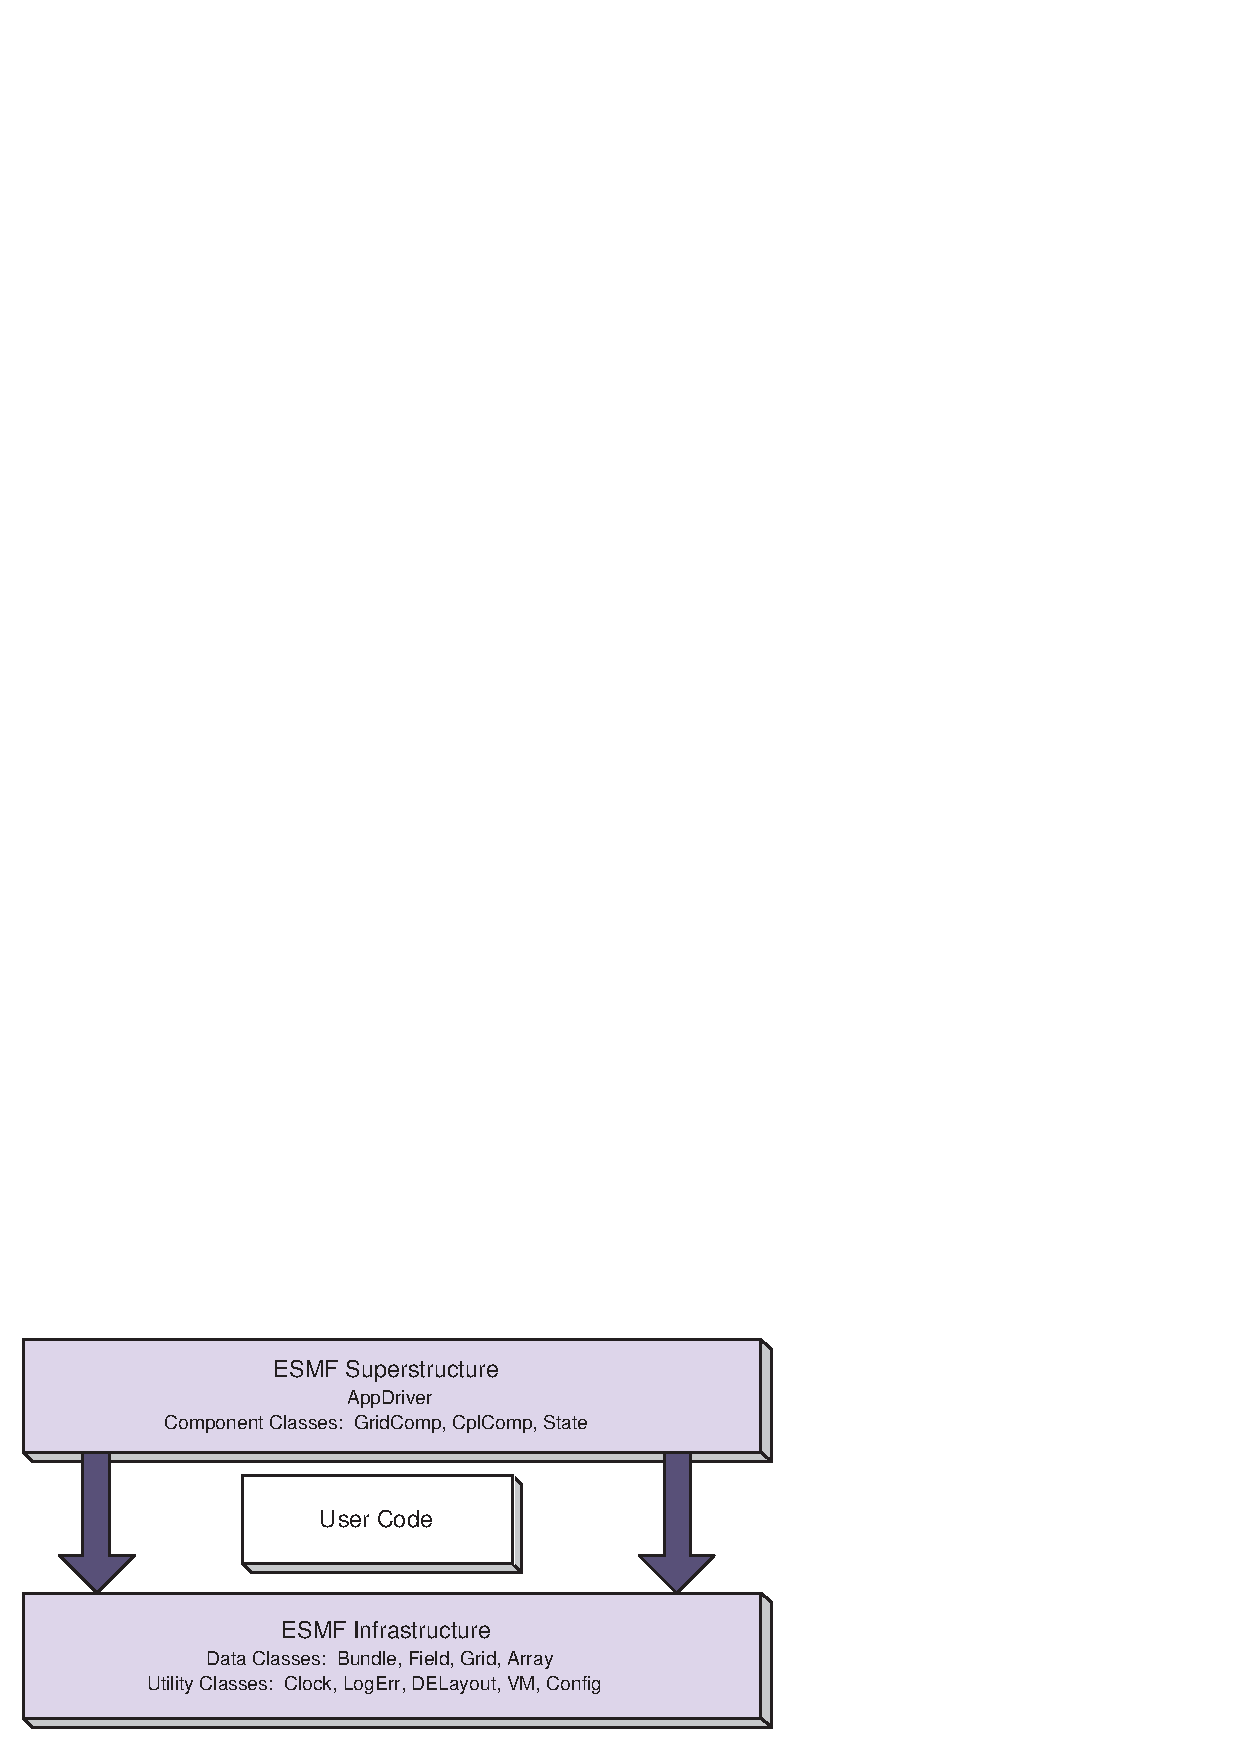
\includegraphics{ESMF_sandwich}}
\end{figure}
\end{center}


%\section{Support}
\section{How to Contact User Support and Find Additional Information}
\label{sec:Support}
The ESMF team can answer questions about the interfaces presented in this 
document.  For user support, please contact 
\htmladdnormallink{esmf\_support@ucar.edu}{mailto:esmf\_support@ucar.edu}.  

The website, \htmladdnormallink{http://www.earthsystemmodeling.org}{http://www.earthsystemmodeling.org}, provide more information of the ESMF project as a whole.
The website includes release notes and known bugs for each version of the
framework, supported platforms, project history, values, and metrics, related projects,
the ESMF management structure, and more.  The \htmladdnormallink
{{\it ESMF User's Guide}}{http://www.earthsystemmodeling.org/esmf\_releases/public/last/ESMF\_usrdoc/} contains build and installation instructions, an overview of the ESMF system and a description of 
how its classes interrelate (this version of the document corresponds to the last public version of the framework).  Also available on the ESMF website is the 
\htmladdnormallink{{\it ESMF Developer's Guide}}{http://www.earthsystemmodeling.org/documents/dev\_guide/} 
that details ESMF procedures and conventions.  
 
\section{How to Submit Comments, Bug Reports, and Feature Requests}
\label{sec:Submission}
\begin{sloppypar}
We welcome input on any aspect of the ESMF project.  Send
questions and comments to 
\htmladdnormallink{esmf\_support@ucar.edu}
{mailto:esmf\_support@ucar.edu}.
\end{sloppypar}







%\section{Document Conventions}
%\section{Conventions}
\label{sec:conventions}

\subsection{Typeface and Diagram Conventions}


The following conventions for fonts and capitalization are used
in this and other ESMF documents. \newline

\begin{tabular}{lll}
{\bf Style} & {\bf Meaning} & {\bf Example} \\ \hline
{\it italics}  & documents & {\it ESMF Reference Manual}\\
{\tt courier}  & code fragments & {\tt ESMF\_TRUE}\\
{\tt courier()}  & ESMF method name & {\tt ESMF\_FieldGet()} \\
{\bf boldface} & first definitions & An {\bf address space} is ...\\
{\bf boldface} & web links and tabs & {\bf Developers} tab on the website \\
{Capitals}     & ESMF class name & DataMap \\
\end{tabular} 
 
ESMF class names frequently coincide with words commonly
used within the Earth system domain (field, grid, component, array, 
etc.)  The convention we adopt in this manual is that if a word is 
used in the context of an ESMF class name it is capitalized, and 
if the word is used in a more general context it remains in lower 
case.  We would write, for example, that an ESMF Field class 
represents a physical field.  

%Section and subsection titles should follow the convention of capitalizing
%all words in the title except for little words, such as: a, an, the, but, 
%as, if, and, or, nor, or prepositions.  However, the subsubsection titles 
%should only capitalize the first word and any other proper nouns, such as 
%ESMF class names.  There should be no punction at the end of any title, whether 
%it be a section, subsection, or subsubsection.

Diagrams are drawn using the Unified Modeling Language (UML).  UML 
is a visual tool that can illustrate the structure of 
classes, define relationships between classes, and describe sequences
of actions.  A reader interested in more detail can refer to a 
text such as {\it The Unified Modeling Language Reference Manual.}
 \cite{uml}



\subsection{Method Name and Argument Conventions}

Method names begin with {\tt ESMF\_}, followed by the class name, 
followed by the name of the operation being performed.  Each new 
word is capitalized.  Although Fortran interfaces are not case-sensitive,
we use case to help parse multi-word names.  

For method arguments that are multi-word, the first word is lower
case and subsequent words begin with upper case.  ESMF class 
names (including typed flags) are an exception.  When multi-word 
class names appear in argument lists, all letters after the first 
are lower case.  The first letter is lower case if the class is the
first word in the argument and upper case otherwise.  For 
example, in an argument list the DELayout class name may appear 
as {\tt delayout} or {\tt srcDelayout}.

Most Fortran calls in the ESMF are subroutines, with 
any returned values passed through the interface.  For the sake of 
convenience, some ESMF calls are written as functions.

A typical ESMF call looks like this:

\begin{verbatim}
call ESMF_<ClassName><Operation>(classname, firstArgument, 
           secondArgument, ..., rc)
\end{verbatim}

where \newline
{\tt <ClassName>} is the class name, \newline
{\tt <Operation>} is the name of the action to be performed, \newline 
{\tt classname} is a variable of the derived type associated 
with the class, \newline
the {\tt arg*} arguments are whatever other variables are required 
for the operation, \newline
and {\tt rc} is a return code. \newline





\newpage
%\section{API Overview}
% $Id$
%
% Earth System Modeling Framework
% Copyright 2002-2020, University Corporation for Atmospheric Research, 
% Massachusetts Institute of Technology, Geophysical Fluid Dynamics 
% Laboratory, University of Michigan, National Centers for Environmental 
% Prediction, Los Alamos National Laboratory, Argonne National Laboratory, 
% NASA Goddard Space Flight Center.
% Licensed under the University of Illinois-NCSA License.

\section{The ESMF Application Programming Interface}

The ESMF Application Programming Interface (API) is based on the
object-oriented programming concept of a {\bf class}.  A class is a 
software construct that is used for grouping a set of related variables 
together with the subroutines and functions that operate on them.  We 
use classes in ESMF because they help to organize the code, and often 
make it easier to maintain and understand.  A particular instance
of a class is called an {\bf object}.  For example, Field is an 
ESMF class.  An actual Field called {\tt temperature} is an object. 
That is about as far as we will go into software engineering
terminology.  

The C interface is implemented so that the variables associated
with a class are stored in a C structure.  For example, an 
{\tt ESMC\_Field} structure stores the data array, grid 
information, and metadata associated with a physical field.
The structure for each class is defined in a C header file. 
The operations associated with each class are also
defined in the header files.

The header files for ESMF are bundled together and can be accessed with a 
single {\tt include} statement, {\tt \#include "ESMC.h"}.  By convention,
the C entry points are named using ``ESMC'' as a prefix.

\subsection{Standard Methods and Interface Rules}

ESMF defines a set of standard methods and interface rules that
hold across the entire API.  These are: 

\begin{itemize}

\item
\begin{sloppypar}
{\tt ESMC\_<Class>Create()} and {\tt ESMC\_<Class>Destroy()}, for
creating and destroying objects of ESMF classes that require internal memory
management (- called ESMF deep classes). The {\tt ESMC\_<Class>Create()} method
allocates memory for the object itself and for internal variables, and
initializes variables where appropriate.  It is always written as a
function that returns a derived type instance of the class, i.e. an object.
\end{sloppypar}

\item 
\begin{sloppypar}
{\tt ESMC\_<Class>Set()} and {\tt ESMC\_<Class>Get()}, for setting and 
retrieving a particular item or flag.  In general, these methods are overloaded
for all cases where the item can be manipulated as a name/value pair.  If
identifying the item requires more than a name, or if the class is of
sufficient complexity that overloading in this way would result in an
overwhelming number of options, we define specific
{\tt ESMC\_<Class>Set<Something>()} and {\tt ESMC\_<Class>Get<Something>()}
interfaces.
\end{sloppypar}

\item {\tt ESMC\_<Class>Add()}, {\tt ESMC\_<Class>AddReplace()},
{\tt ESMC\_<Class>Remove()}, and {\tt ESMC\_<Class>Replace()}, for manipulating
objects of ESMF container classes - such as {\tt ESMC\_State} and
{\tt ESMC\_FieldBundle}. For example, the {\tt ESMC\_FieldBundleAdd()}
method adds another Field to an existing FieldBundle object.

\item {\tt ESMC\_<Class>Print()}, for printing the contents of an object to 
standard out.  This method is mainly intended for debugging.

\item {\tt ESMC\_<Class>ReadRestart()} and {\tt ESMC\_<Class>WriteRestart()}, 
for saving the contents of a class and restoring it exactly.  Read
and write restart methods have not yet been implemented for most
ESMF classes, so where necessary the user needs to write restart 
values themselves.

\item 
\begin{sloppypar}
{\tt ESMC\_<Class>Validate()}, for determining whether a class is 
internally consistent.  For example, {\tt ESMC\_FieldValidate()} validates
the internal consistency of a Field object.
\end{sloppypar}

\end{itemize}

\subsection{Deep and Shallow Classes}
\label{sec:deepshallow}

The ESMF contains two types of classes.

{\bf Deep} classes require
{\tt ESMC\_<Class>Create()} and {\tt ESMC\_<Class>Destroy()} calls.
They involve memory allocation, take significant time to set up (due to
memory management) and should not be created in a time-critical portion of code.
Deep objects persist even after the method in which they were created has
returned. Most classes in ESMF, including GridComp, CplComp, State, Fields, FieldBundles, Arrays, ArrayBundles, Grids, and Clocks, fall into this category.

{\bf Shallow} classes do not possess {\tt ESMC\_<Class>Create()}
and {\tt ESMC\_<Class>Destroy()} calls.  They are simply declared
and their values set using an {\tt ESMC\_<Class>Set()} call.  
Examples of shallow classes are Time, TimeInterval, and ArraySpec.  Shallow classes do not take long to set up and can be declared and set within
a time-critical code segment.  Shallow objects stop existing when
the method in which they were declared has returned.  

An exception to this is when a shallow object, such as a Time, 
is stored in a deep object such as a Clock.  The Clock then
carries a copy of the Time in persistent memory.  The Time is
deallocated with the {\tt ESMC\_ClockDestroy()} call.

See Section \ref{sec:overallimpl}, Overall Design and Implementation 
Notes, for a brief discussion of deep and shallow classes from 
an implementation perspective.  For an in-depth look at the design
 and inter-language issues related to deep and shallow classes,
see the \htmladdnormallink{{\it ESMF Implementation Report}}{http://www.earthsystemmodeling.org/documents/IMPL\_repdoc/}.

\subsection{Special Methods}

The following are special methods which, in one case,
are required by any application using ESMF, and in the 
other case must be called by any application that is using 
ESMF Components.

\begin{itemize}

\item {\tt ESMC\_Initialize()} and {\tt ESMC\_Finalize()} are required 
methods that must bracket the use of ESMF within an application.  
They manage the resources required to run ESMF and shut it down
gracefully.  ESMF does not support restarts in the same executable, i.e.
{\tt ESMC\_Initialize()} should not be called after {\tt ESMC\_Finalize()}.
\item {\tt ESMC\_<Type>CompInitialize()}, {\tt ESMC\_<Type>CompRun()}, and 
{\tt ESMC\_<Type>CompFinalize()} are component methods that are used at the 
highest level within ESMF.  {\tt <Type>} may be {\tt <Grid>}, for 
Gridded Components such as oceans or atmospheres, or
{\tt <Cpl>}, for Coupler Components that are used to connect 
them.  The content of these methods is not part of the ESMF.  
Instead the methods call into associated subroutines within 
user code.

\end{itemize}

\subsection{The ESMF Data Hierarchy}

The ESMF API is organized around a hierarchy of classes that
contain model data.  The operations that are performed
on model data, such as regridding, redistribution, and halo 
updates, are methods of these classes.  

The main data classes offered by the ESMF C API, in order of increasing complexity, are:
\begin{itemize}
\item {\bf Array} An ESMF Array is a distributed, multi-dimensional 
array that can carry information such as its type, kind, rank, and 
associated halo widths.  It contains a reference to a native language array.
\item {\bf Field}  A Field represents a physical scalar or vector field.
It contains a reference to an Array along with grid information and metadata.
\item {\bf State}  A State represents the collection of data that a 
Component either requires to run (an Import State) or can make 
available to other Components (an Export State).
States may contain references to Arrays, ArrayBundles, Fields,
FieldBundles, or other States. 
\item {\bf Component}  A Component is a piece of software 
with a distinct function.  ESMF currently recognizes two types 
of Components.  Components that represent a physical domain 
or process, such 
as an atmospheric model, are called Gridded Components since they are 
usually discretized on an underlying grid.  The Components 
responsible for regridding and transferring data between Gridded 
Components are called Coupler Components.  Each Component
is associated with an Import and an Export State.  Components
can be nested so that simpler Components are contained within more
complex ones.

\end{itemize}

Underlying these data classes are native language arrays.  ESMF Arrays 
and Fields can be queried for the C pointer to the actual data.  You can
perform communication operations either on the ESMF data objects or
directly on C arrays through the VM class, which serves 
as a unifying wrapper for distributed and shared memory communication 
libraries.

\subsection{ESMF Spatial Classes}
\label{sec:spatialclasses}

Like the hierarchy of model data classes, ranging from the 
simple to the complex, ESMF is organized around a hierarchy of
classes that represent different spaces associated with a computation.
Each of these spaces can be manipulated, in order to give
the user control over how a computation is executed.  For Earth system
models, this hierarchy starts with the address space associated
with the computer and extends to the physical region described by
the application.   The main spatial classes in ESMF, from
those closest to the machine to those closest to the application, are:

\begin{itemize}

\item The {\bf Virtual Machine}, or {\bf VM} The ESMF VM is an 
abstraction of a parallel computing environment that encompasses 
both shared and distributed memory, single and multi-core systems.
Its primary purpose is resource allocation and management. Each Component
runs in its own VM, using the resources it defines. The elements of a VM
are {\bf Persistent Execution Threads}, or {\bf PETs}, that are
executing in {\bf Virtual Address Spaces}, or {\bf VASs}. A simple
case is one in which every PET is associated with a single MPI process.
In this case every PET is executing in its own private VAS. If Components
are nested, the parent Component allocates a subset of its PETs to its
children. The children have some flexibility, subject to the constraints of
the computing environment, to decide how they want to use the
resources associated with the PETs they've received.

\item {\bf DELayout}  A DELayout represents a data decomposition
(we also refer to this as a distribution).  Its
basic elements are {\bf Decomposition Elements}, or {\bf DEs}.  
A DELayout associates a set of DEs with the PETs in a VM.  DEs are not
necessarily one-to-one with PETs.  For cache blocking,
or user-managed multi-threading, more DEs than PETs may be defined.
Fewer DEs than PETs may also be defined if an application requires it.

The current ESMF C API does not provide user access to the DELayout class.

\item {\bf DistGrid}  A DistGrid represents the index space
associated with a grid.  It is a useful abstraction because
often a full specification of grid coordinates is not necessary
to define data communication patterns.  The DistGrid contains
information about the sequence and connectivity of data points,
which is sufficient information for many operations.  Arrays
are defined on DistGrids.

\item {\bf Array} An Array defines how the index space described
in the DistGrid is associated with the VAS of each PET. This association
considers the type, kind and rank of the indexed data. Fields are
defined on Arrays.

\item {\bf Grid}  A Grid is an abstraction for a logically rectangular
region in physical space.  It associates a coordinate system, a set of
coordinates, and a topology to a collection of grid cells.  Grids in ESMF
are comprised of DistGrids plus additional coordinate information.

\item {\bf Mesh}  A Mesh provides an abstraction for an unstructured 
grid.  Coordinate information is set in nodes, which represent
vertices or corners.  Together the nodes establish the boundaries
of mesh elements or cells.

\item {\bf LocStream}  A LocStream is an abstraction for a set of 
unstructured data points without any topological relationship to each 
other.

\item {\bf Field}  A Field may contain more dimensions than the 
Grid that it is discretized on.  For example, for convenience 
during integration, a user may want to define a single Field object 
that holds snapshots of data at multiple times.  Fields also 
keep track of the stagger location of a Field data point within its 
associated Grid cell.

\end{itemize}

\subsection{ESMF Maps}

In order to define how the index spaces of the spatial classes relate
to each other, we require either implicit rules (in which case the
relationship between spaces is defined by default), or special Map arrays
that allow the user to specify the desired association.  The form of the 
specification is usually that the position of the array element carries
information about the first object, and the value of the array element carries
information about the second object.  ESMF includes a {\tt distGridToArrayMap},
a {\tt gridToFieldMap}, a {\tt distGridToGridMap}, and others.

\subsection{ESMF Specification Classes}

It can be useful to make small packets
of descriptive parameters.  ESMF has one of these:
\begin{itemize}
\item {\bf ArraySpec}, for storing the specifics, such as type/kind/rank,
of an array.
\end{itemize}

\subsection{ESMF Utility Classes}

There are a number of utilities in ESMF that can be used independently.
These are:
\begin{itemize}
\item {\bf Attributes}, for storing metadata about Fields,
FieldBundles, States, and other classes.
(Not currently available through the ESMF C API.)
\item {\bf TimeMgr}, for calendar, time, clock and alarm functions.
\item {\bf LogErr}, for logging and error handling.
\item {\bf Config}, for creating resource files that can replace namelists
as a consistent way of setting configuration parameters.
\end{itemize}

\section{Integrating ESMF into Applications}

Depending on the requirements of the application, the user may 
want to begin integrating ESMF in either a top-down or bottom-up 
manner.  In the top-down approach, tools at the superstructure 
level are used to help reorganize and structure the interactions
among large-scale components in the application.  It is appropriate
when interoperability is a primary concern; for example, when 
several different versions or implementations of components are going 
to be swapped in, or a particular component is going to be used 
in multiple contexts.  Another reason for deciding on a top-down 
approach is that the application contains legacy code that for 
some reason (e.g., intertwined functions, very large,
highly performance-tuned, resource limitations) there is little 
motivation to fully restructure.  The superstructure can usually be 
incorporated into such applications in a way that is non-intrusive.

In the bottom-up approach, the user selects desired utilities 
(data communications, calendar management, performance profiling,
logging and error handling, etc.) from the ESMF infrastructure 
and either writes new code using them, introduces them into 
existing code, or replaces the functionality in existing code 
with them.  This makes sense when maximizing code reuse and 
minimizing maintenance costs is a goal.  There may be a specific
need for functionality or the component writer may be starting
from scratch.  The calendar management utility is a popular
place to start.

\subsection{Using the ESMF Superstructure}

The following is a typical set of steps involved in adopting
the ESMF superstructure.  The first two tasks, which occur 
before an ESMF call is ever made, have the potential to be 
the most difficult and time-consuming.  They are the work 
of splitting an application into components and ensuring that
each component has well-defined stages of execution.  ESMF
aside, this sort of code structure helps to promote application
clarity and maintainability, and the effort put into it is likely
to be a good investment.

\begin{enumerate}

\item Decide how to organize the application as discrete Gridded 
and Coupler Components.  This might involve reorganizing code
so that individual components are cleanly separated and their 
interactions consist of a minimal number of data exchanges.

\item Divide the code for each component into initialize, run, and
finalize methods.  These methods can be multi-phase, e.g., 
{\tt init\_1, init\_2}.

\item Pack any data that will be transferred between components
into ESMF Import and Export State data structures.  This is done
by first wrapping model data in either ESMF Arrays or Fields.
Arrays are simpler to create and use than Fields, but carry less
information and have a more limited range of operations.
These Arrays and Fields are then added to Import and
Export States.  They may be packed into ArrayBundles or
FieldBundles first, for more efficient communications.
Metadata describing the model data can also be added.
At the end of this step, the data to be transferred between
components will be in a compact and largely self-describing
form.

\item Pack time information into ESMF time management data 
structures.

\item Using code templates provided in the ESMF distribution, create
ESMF Gridded and Coupler Components to represent each component
in the user code.

\item Write a set services routine that sets ESMF entry 
points for each user component's initialize, run, and finalize 
methods.

\item Run the application using an ESMF Application Driver.

\end{enumerate} 


\subsection{Constants}

Named constants are used throughout ESMF to specify the values of many 
arguments with multiple well defined values in a consistent way.  These 
constants are defined by a derived type that follows this pattern:

\begin{verbatim}
ESMF_<CONSTANT_NAME>_Flag
\end{verbatim}

The values of the constant are then specified by this pattern:

\begin{verbatim}
ESMF_<CONSTANT_NAME>_<VALUE1>
ESMF_<CONSTANT_NAME>_<VALUE2>
ESMF_<CONSTANT_NAME>_<VALUE3>
...
\end{verbatim}

A master list of all available constants can be found in section 
\ref{const:cmaster}.

\section{Overall Rules and Behavior}

\subsection{Local and Global Views and Associated Conventions}

ESMF data objects such as Fields are distributed over
DEs, with each DE getting a portion of the data.  Depending
on the task, a local or global view of the object may be
preferable.  In a local view, data indices start with the first
element on the DE and end with the last element on the same DE.
In a global view, there is an assumed or specified order to
the set of DEs over which the object is distributed.  Data
indices start with the first element on the first DE, and
continue across all the elements in the sequence of DEs.
The last data index represents the number of elements in the
entire object.  The DistGrid provides the mapping between
local and global data indices.

The convention in ESMF is that entities with a global view
have no prefix.  Entities with a DE-local (and in some cases,
PET-local) view have the prefix ``local.''

Just as data is distributed over DEs, DEs themselves can be
distributed over PETs.  This is an advanced feature for users
who would like to create multiple local chunks of data, for
algorithmic or performance reasons.
Local DEs are those DEs that are located on the local PET.
Local DE labeling always starts at 0 and goes to localDeCount-1,
where localDeCount is the number of DEs on the local PET.
Global DE numbers also start at 0 and go to deCount-1.
The DELayout class provides the mapping between local
and global DE numbers. 

\subsection{Allocation Rules}

The basic rule of allocation and deallocation for the ESMF is:
whoever allocates it is responsible for deallocating it.

ESMF methods that allocate their own space for data will
deallocate that space when the object is destroyed. 
Methods which accept a user-allocated buffer, for example
{\tt ESMC\_FieldCreate()} with the {\tt ESMF\_DATACOPY\_REFERENCE} flag,
will not deallocate that buffer at the time the object is
destroyed.  The user must deallocate the buffer
when all use of it is complete.

Classes such as Fields, FieldBundles, and States may have Arrays, 
Fields, Grids and FieldBundles created externally and associated with
them.  These associated items are not destroyed along with the rest  
of the data object since it is possible for the items to be added 
to more than one data object at a time (e.g. the same Grid could 
be part of many Fields).  It is the user's responsibility to delete 
these items when the last use of them is done.

\subsection{Assignment, Equality, Copying and Comparing Objects}

The equal sign assignment has not been overloaded in ESMF, thus resulting in
the standard C behavior. This behavior has been documented as the first
entry in the API documentation section for each ESMF class. For deep ESMF
objects the assignment results in setting an alias the the same ESMF object
in memory. For shallow ESMF objects the assignment is essentially a equivalent
to a copy of the object. For deep classes the equality operators have been
overloaded to test for the alias condition as a counter part to the assignment
behavior. This and the not equal operator are documented following the
assignment in the class API documentation sections. 

Deep object copies are implemented as a special variant of the
{\tt ESMC\_<Class>Create()} methods. It takes an existing deep object as
one of the required arguments. At this point not all deep classes have
{\tt ESMC\_<Class>Create()} methods that allow object copy.

Due to the complexity of deep classes there are many aspects when comparing two
objects of the same class. ESMF provide {\tt ESMC\_<Class>Match()} methods,
which are functions that return a class specific match flag. At this point not
all deep classes have {\tt ESMC\_<Class>Match()} methods that allow deep object
comparison.

%\subsection{Attributes}
%
%Attributes are (name, value) pairs, where
%the name is a character string and the value can be either a single
%value or list of {\tt int}, {\tt double}, or {\tt char *} values.
%Attributes can be associated with Fields, FieldBundles, and States. 
%Mixed types are not allowed in a single attribute, and all attribute
%names must be unique within a single object.    Attributes are set
%by name, and can be retrieved either directly by name or by querying
%for a count of attributes and retrieving names and values
%by index number.



\section{Overall Design and Implementation Notes}
\label{sec:overallimpl}

\begin{enumerate}

\item {\bf Deep and shallow classes.}  The deep and shallow classes 
described in Section \ref{sec:deepshallow} differ in how and where they
are allocated within a multi-language implementation environment.  We
distinguish between the implementation language, which is the language
a method is written in, and the calling language, which is the language
that the user application is written in.  Deep classes are allocated 
off the process heap by the implementation language.  Shallow classes
are allocated off the stack by the calling language.  

\item {\bf Base class.} All ESMF classes are built upon a Base class,
which holds a small set of system-wide capabilities.  

\end{enumerate}

%\subsection{Overall Design and Implementation Notes}
%% $Id$

\section{Overall Design and Implementation Notes}
\label{sec:overallimpl}

\begin{enumerate}

\item {\bf Deep and shallow classes.}  The deep and shallow classes 
described in Section \ref{sec:deepshallow} differ in how and where they
are allocated within a multi-language implementation environment.  We
distinguish between the implementation language, which is the language
a method is written in, and the calling language, which is the language
that the user application is written in.  Deep classes are allocated 
off the process heap by the implementation language.  Shallow classes
are allocated off the stack by the calling language.  

\item {\bf Base class.} All ESMF classes are built upon a Base class,
which holds a small set of system-wide capabilities.  

\end{enumerate}

%\subsection{Overall Restrictions and Future Work}
%% $Id$

\section{Overall Restrictions and Future Work}
\label{sec:overallrest}

\begin{enumerate}

\item {\bf 32-bit integer limitations.} In general, Fortran array bounds should
be limited to 2**31-1 elements or less.  This is due to the Fortran-95
limitation of returning default sized (e.g., 32 bit) integers for array bound
and size inquiries, and consequent ESMF use of default sized integers for
holding these values.

\end{enumerate}

\newpage
\begin{htmlonly}
\addcontentsline{toc}{part}{Applications}
\end{htmlonly}
\part{Applications}
\label{part:CApplications}
% $Id$

The main product delivered by ESMF is the ESMF library that allows application
developers to write programs based on the ESMF Fortran or C APIs. In addition to 
the programming library, ESMF distributions come with a small set of applications
that are of general interest to the community. These applications utilize
the ESMF library to implement features such as printing general information
about the ESMF installation, or generating regrid weight files. The provided
ESMF applications are intended to be used as standard command line tools.

The bundled ESMF applications are built and installed during the usual ESMF 
installation process, which is described in detail in the ESMF User's Guide 
section "Building and Installing the ESMF". After installation, the
applications will be located in the {\tt ESMF\_APPSDIR} directory, which can 
be found as a Makefile variable in the {\tt esmf.mk} file. The {\tt esmf.mk} 
file can be found in the {\tt ESMF\_INSTALL\_LIBDIR} directory after a 
successful installation.  The ESMF User's Guide discusses the {\tt esmf.mk} 
mechanism to access the bundled applications in more detail in section 
"Using Bundled ESMF Applications".

Refer to the "Application" section of the ESMF Fortran reference manual
for more information. In addition, each application supports the standard 
\verb+ --help + command line argument, providing a brief description of 
how to invoke the program.


\newpage
\begin{htmlonly}
\addcontentsline{toc}{part}{Superstructure}
\end{htmlonly}
\part{Superstructure}
\label{part:Superstructure}
\newpage
%\section{Overview of Superstructure}
% $Id$
%
% Earth System Modeling Framework
% Copyright 2002-2020, University Corporation for Atmospheric Research, 
% Massachusetts Institute of Technology, Geophysical Fluid Dynamics 
% Laboratory, University of Michigan, National Centers for Environmental 
% Prediction, Los Alamos National Laboratory, Argonne National Laboratory, 
% NASA Goddard Space Flight Center.
% Licensed under the University of Illinois-NCSA License.

\section{Overview of Superstructure}

ESMF superstructure classes define an architecture for assembling
Earth system applications from modeling {\bf components}.  A component
may be defined in terms of the physical domain that it represents,
such as an atmosphere or sea ice model.  It may also be defined in terms
of a computational function, such as a data assimilation system.
Earth system research often requires that such components be {\bf coupled} 
together to create an application.  By coupling we mean the data 
transformations and, on parallel computing systems, data transfers, 
that are necessary to allow data from one component to be utilized by 
another.  ESMF offers regridding methods and other tools to simplify 
the organization and execution of inter-component data exchanges.  

In addition to components defined at the level of major physical 
domains and computational functions, components may be defined that 
represent smaller computational functions within larger components, 
such as the transformation of data between the physics and dynamics 
in a spectral atmosphere model, 
or the creation of nested higher resolution regions 
within a coarser grid.  The objective is to couple components at varying 
scales both flexibly and efficiently.  ESMF encourages a hierarchical
application structure, in which large components branch into 
smaller sub-components (see Figure \ref{fig:GEOS5}).  ESMF also makes 
it easier for the same component to be used in multiple contexts 
without changes to its source code.

\begin{center}  
\begin{tabular}{|p{6in}|}
\hline
\vspace{.01in}
{\bf Key Features} \\[.01in]
Modular, component-based architecture. \\
Hierarchical assembly of components into applications.\\
Use of components in multiple contexts without modification.\\
Sequential or concurrent component execution.\\
Single program, multiple datastream (SPMD) applications for 
maximum portability and reconfigurability.\\
Multiple program, multiple datastream (MPMD) option for 
flexibility.\\ [.03in] \hline
\end{tabular}
\end{center}

\subsection{Superstructure Classes}

There are a small number of classes in the ESMF superstructure:

\begin{itemize}
\item {\bf Component}  An ESMF component has two parts, one that is 
supplied by ESMF and one that is supplied by the user.  The
part that is supplied by the framework is an ESMF derived type that
is either a Gridded Component ({\bf GridComp}) or a Coupler 
Component ({\bf CplComp}).  A Gridded Component typically represents
a physical domain in which data is associated with one or more 
grids - for example, a sea ice model.  A Coupler Component 
arranges and executes data transformations and transfers between
one or more Gridded Components. Gridded Components and Coupler 
Components have standard methods, which include initialize, run,
and finalize.  These methods can be multi-phase.

The second part of an ESMF Component is user code, such as a
model or data assimilation system.  Users set entry points 
within their code so that it is callable by the framework.  
In practice, setting entry points means that within user code 
there are calls to ESMF methods that associate the name of a 
Fortran subroutine with a corresponding standard ESMF operation.  
For example, a user-written initialization routine called 
{\tt myOceanInit} might be associated with the standard 
initialize routine of an ESMF Gridded Component named ``myOcean'' 
that represents an ocean model.

\item {\bf State}  ESMF Components exchange information with other 
Components only through States.  A State is an ESMF derived
type that can contain Fields, FieldBundles, Arrays, ArrayBundles,
and other States.  A Component is associated with two States, an 
{\bf Import State} and an {\bf Export State}.  Its Import State 
holds the data that it receives from other Components.  
Its Export State contains data that it makes available to 
other Components. 

\end{itemize}

An ESMF coupled application typically involves a parent Gridded Component, 
two or more child Gridded Components and one or more Coupler 
Components. 

The parent Gridded Component is responsible for creating the child 
Gridded Components that are exchanging data, for creating the Coupler, 
for creating the necessary Import and Export States, and for 
setting up the desired sequencing.  The application's ``main'' routine
calls the parent Gridded Component's initialize, run, and finalize 
methods in order to execute the application.  For each of these
standard methods, the parent Gridded Component in turn calls the 
corresponding methods in the child Gridded Components and the 
Coupler Component.  For example, consider a simple coupled 
ocean/atmosphere simulation.  When the initialize method of the 
parent Gridded Component is called by the application, it in turn 
calls the initialize methods of its child atmosphere and ocean 
Gridded Components, and the initialize method of an 
ocean-to-atmosphere Coupler Component.  Figure \ref{fig:appunit}
shows this schematically.

\begin{center}
\begin{figure}
\caption{ESMF enables applications such as the atmospheric general
circulation model GEOS-5 to be structured hierarchically, and 
reconfigured and extended easily.  Each box in this diagram is an
ESMF Gridded Component.}
\label{fig:GEOS5}
\scalebox{0.9}{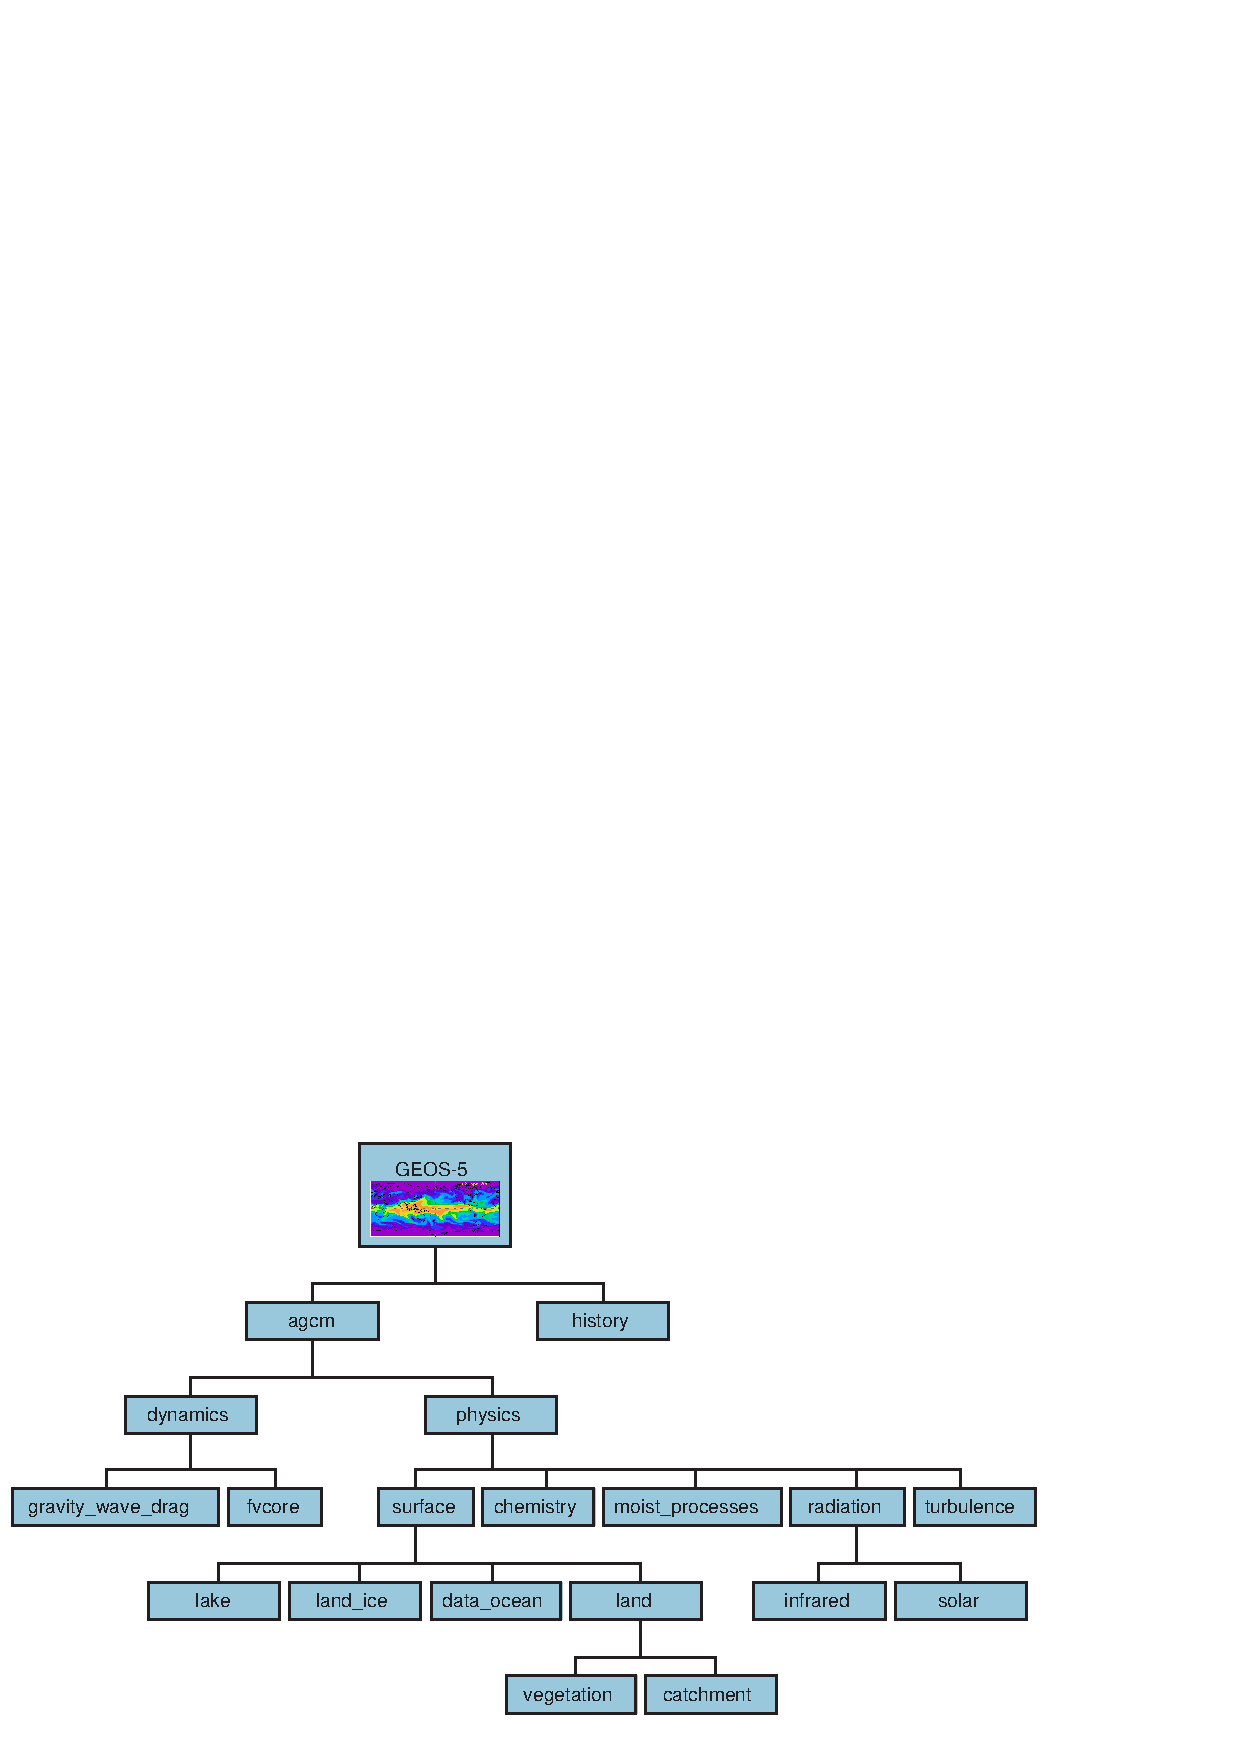
\includegraphics{ESMF_GEOS5}}
\end{figure}
\end{center}

\subsection{Hierarchical Creation of Components}
\label{sec:hierarchy}

Components are allocated computational resources in the form of
{\bf Persistent Execution Threads}, or {\bf PET}s.  A list of a Component's
PETs is contained in a structure called a {\bf Virtual Machine},
or {\bf VM}.  The VM also contains information about the topology and
characteristics of the underlying computer.
Components are created hierarchically, with parent Components creating
child Components and allocating some or all of their PETs to each one.
By default ESMF creates a new VM for each child Component, which 
allows Components to tailor their VM resources to match their needs.
In some cases, a child may want to share its parent's VM - ESMF
supports this, too.

A Gridded Component may exist across all the PETs in an application. 
A Gridded Component may also reside on a subset of PETs in an
application.  These PETs may wholly coincide with, be wholly contained
within, or wholly contain another Component.

\begin{center}
\begin{figure}
\caption{A call to a standard ESMF initialize (run, finalize) method
by a parent component triggers calls to initialize (run, finalize)
all of its child components.}
\label{fig:appunit}
\scalebox{1.0}{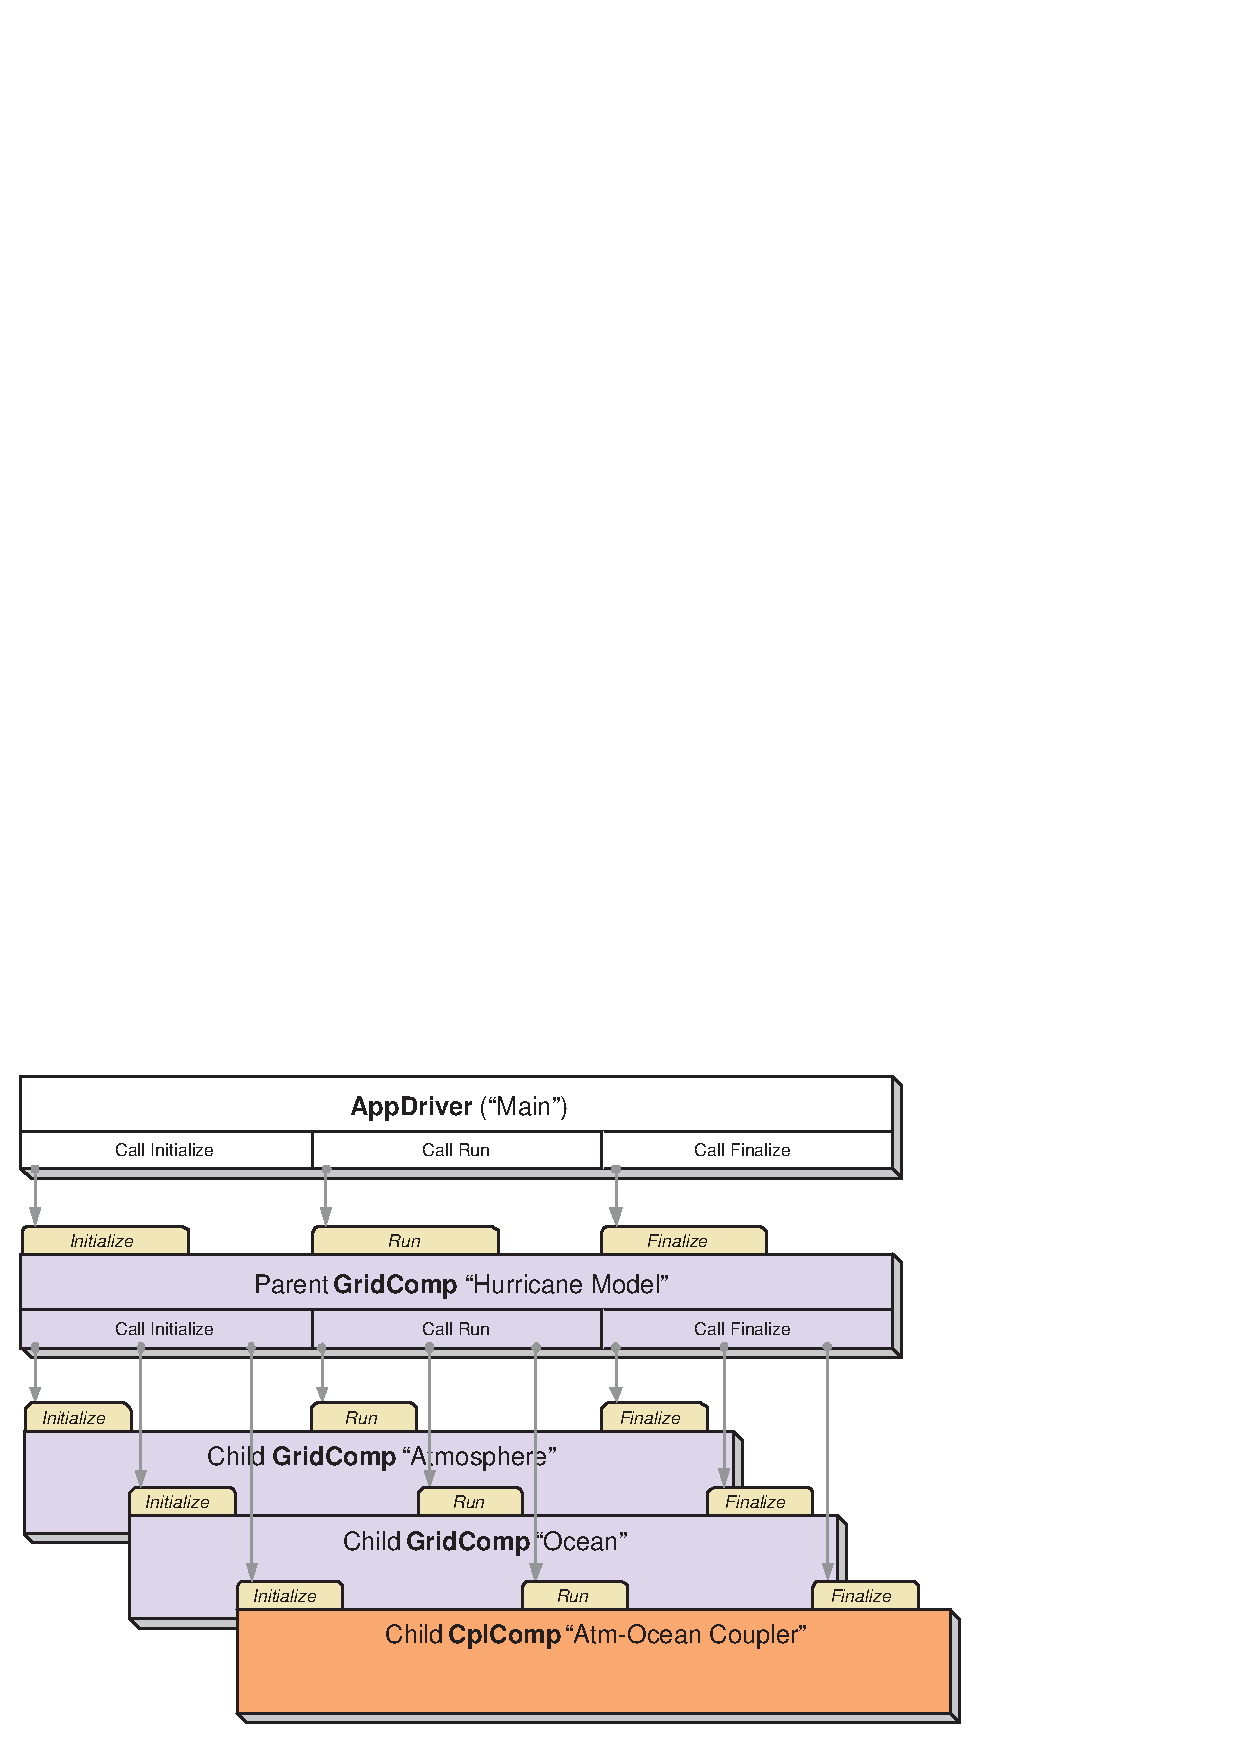
\includegraphics{ESMF_appunit}}
\end{figure}
\end{center}

\subsection{Sequential and Concurrent Execution of Components}
\label{sec:concurrency}

When a set of Gridded Components and a Coupler runs in sequence
on the same set of PETs the application is executing in a {\bf sequential}
mode. When Gridded Components are created and run on mutually exclusive
sets of PETs, and are coupled by a Coupler Component that extends over
the union of these sets, the mode of execution is {\bf concurrent}.

Figure \ref{fig:serial} illustrates a typical configuration for 
a simple coupled sequential
application, and Figure \ref{fig:concurrent} shows a possible 
configuration for the same application running in a concurrent mode.

Parent Components can select if and when to wait for concurrently
executing child Components, synchronizing only when required.

It is possible for ESMF applications to contain some Component sets
that are executing sequentially and others that are executing concurrently.
We might have, for example, atmosphere and land Components created
on the same subset of PETs, ocean and sea ice Components created on
the remainder of PETs, and a Coupler created across all the PETs in
the application.

\begin{center}
\begin{figure}
\caption{Schematic of the run method of a coupled application, with an
``Atmosphere'' and an ``Ocean'' Gridded Component running sequentially with 
an ``Atm-Ocean Coupler.''  The top-level ``Hurricane Model'' 
Gridded Component contains the sequencing information and time 
advancement loop.  The application driver, Coupler, and all Gridded Components 
are distributed over nine PETs.}
\label{fig:serial}
\scalebox{1.0}{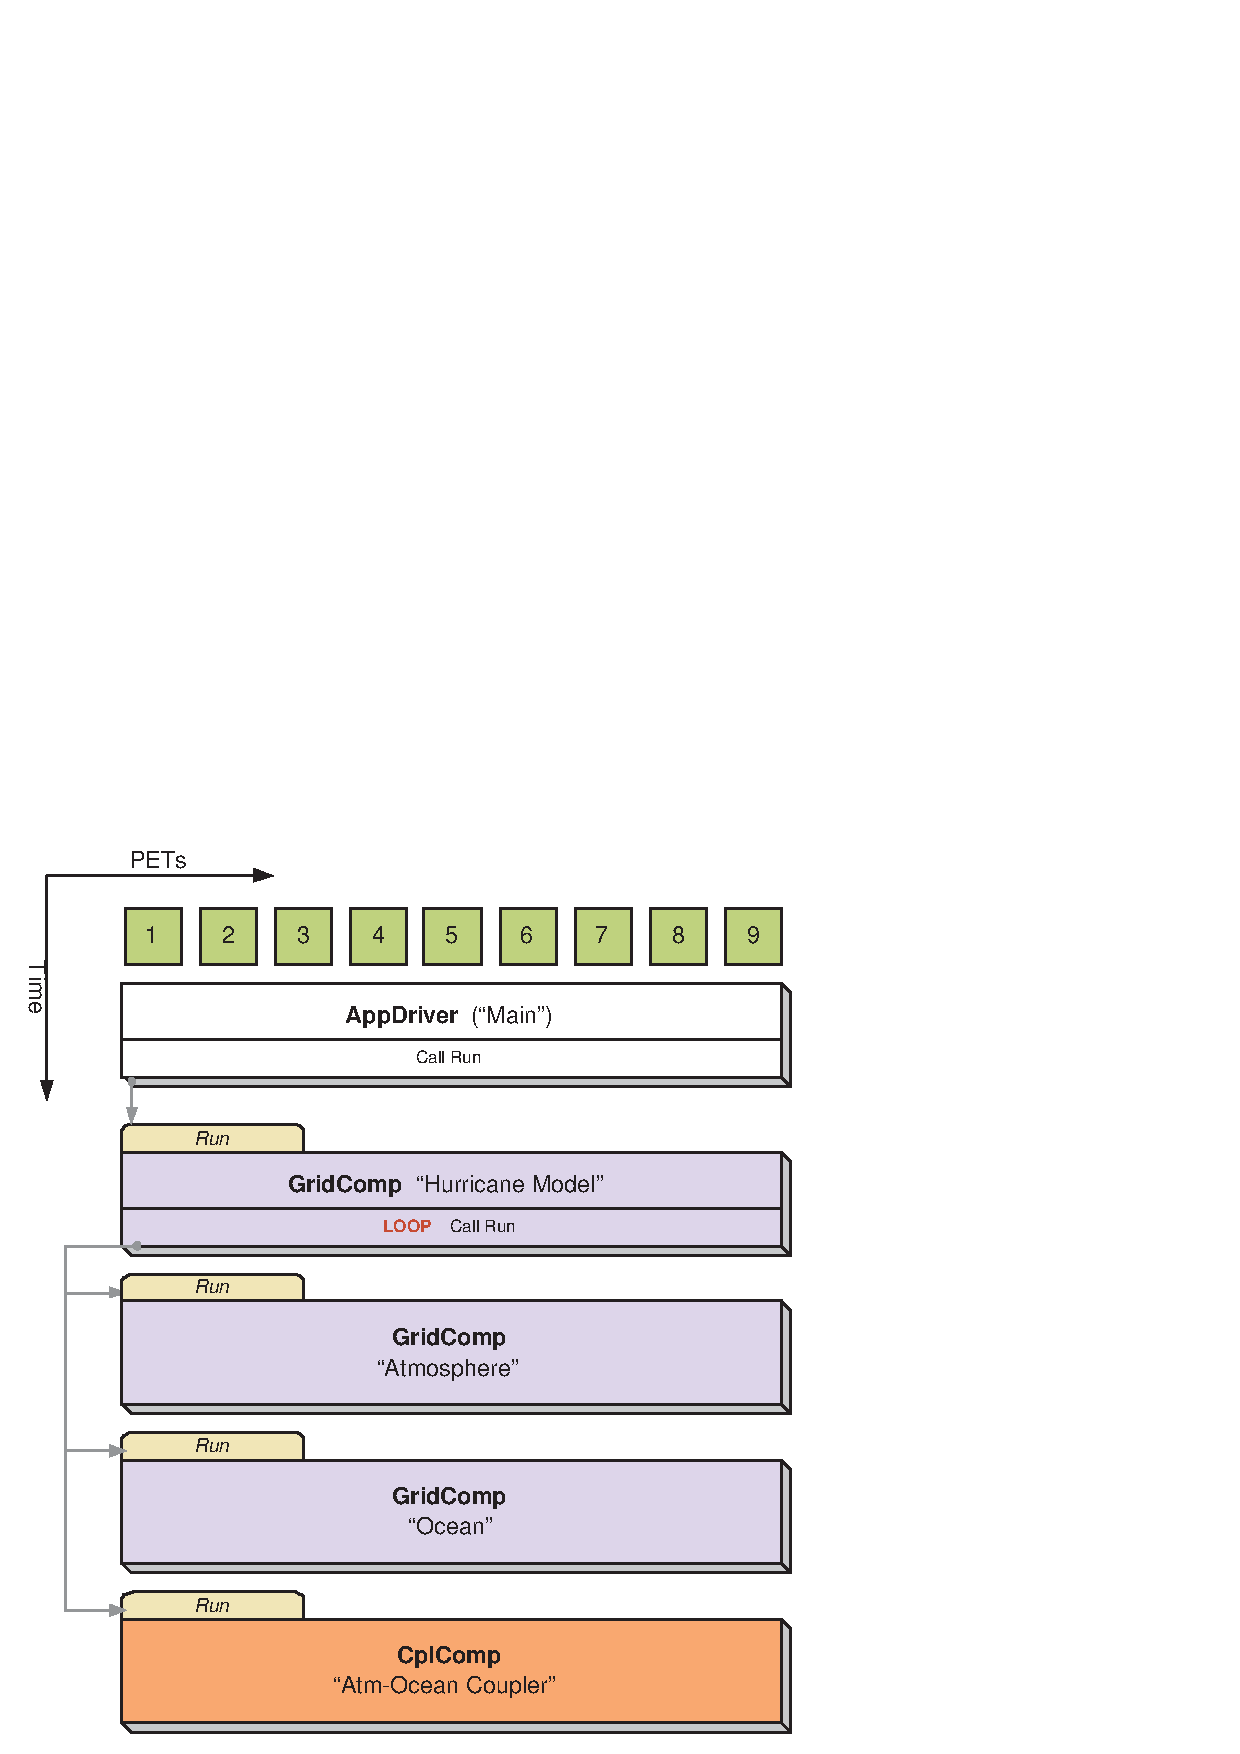
\includegraphics{ESMF_serial}}
\end{figure}
\end{center}

\begin{center}
\begin{figure}
\caption{Schematic of the run method of a coupled application, with an
``Atmosphere'' and an ``Ocean'' Gridded Component running concurrently with 
an ``Atm-Ocean Coupler.''  The top-level ``Hurricane Model'' 
Gridded Component contains the sequencing information and time 
advancement loop.  The application driver, Coupler, and top-level ``Hurricane
Model'' Gridded Component are distributed over nine PETs.  The
``Atmosphere'' Gridded Component is distributed over three PETs and
the ``Ocean'' Gridded Component is distributed over six PETs.}
\label{fig:concurrent}
\scalebox{1.0}{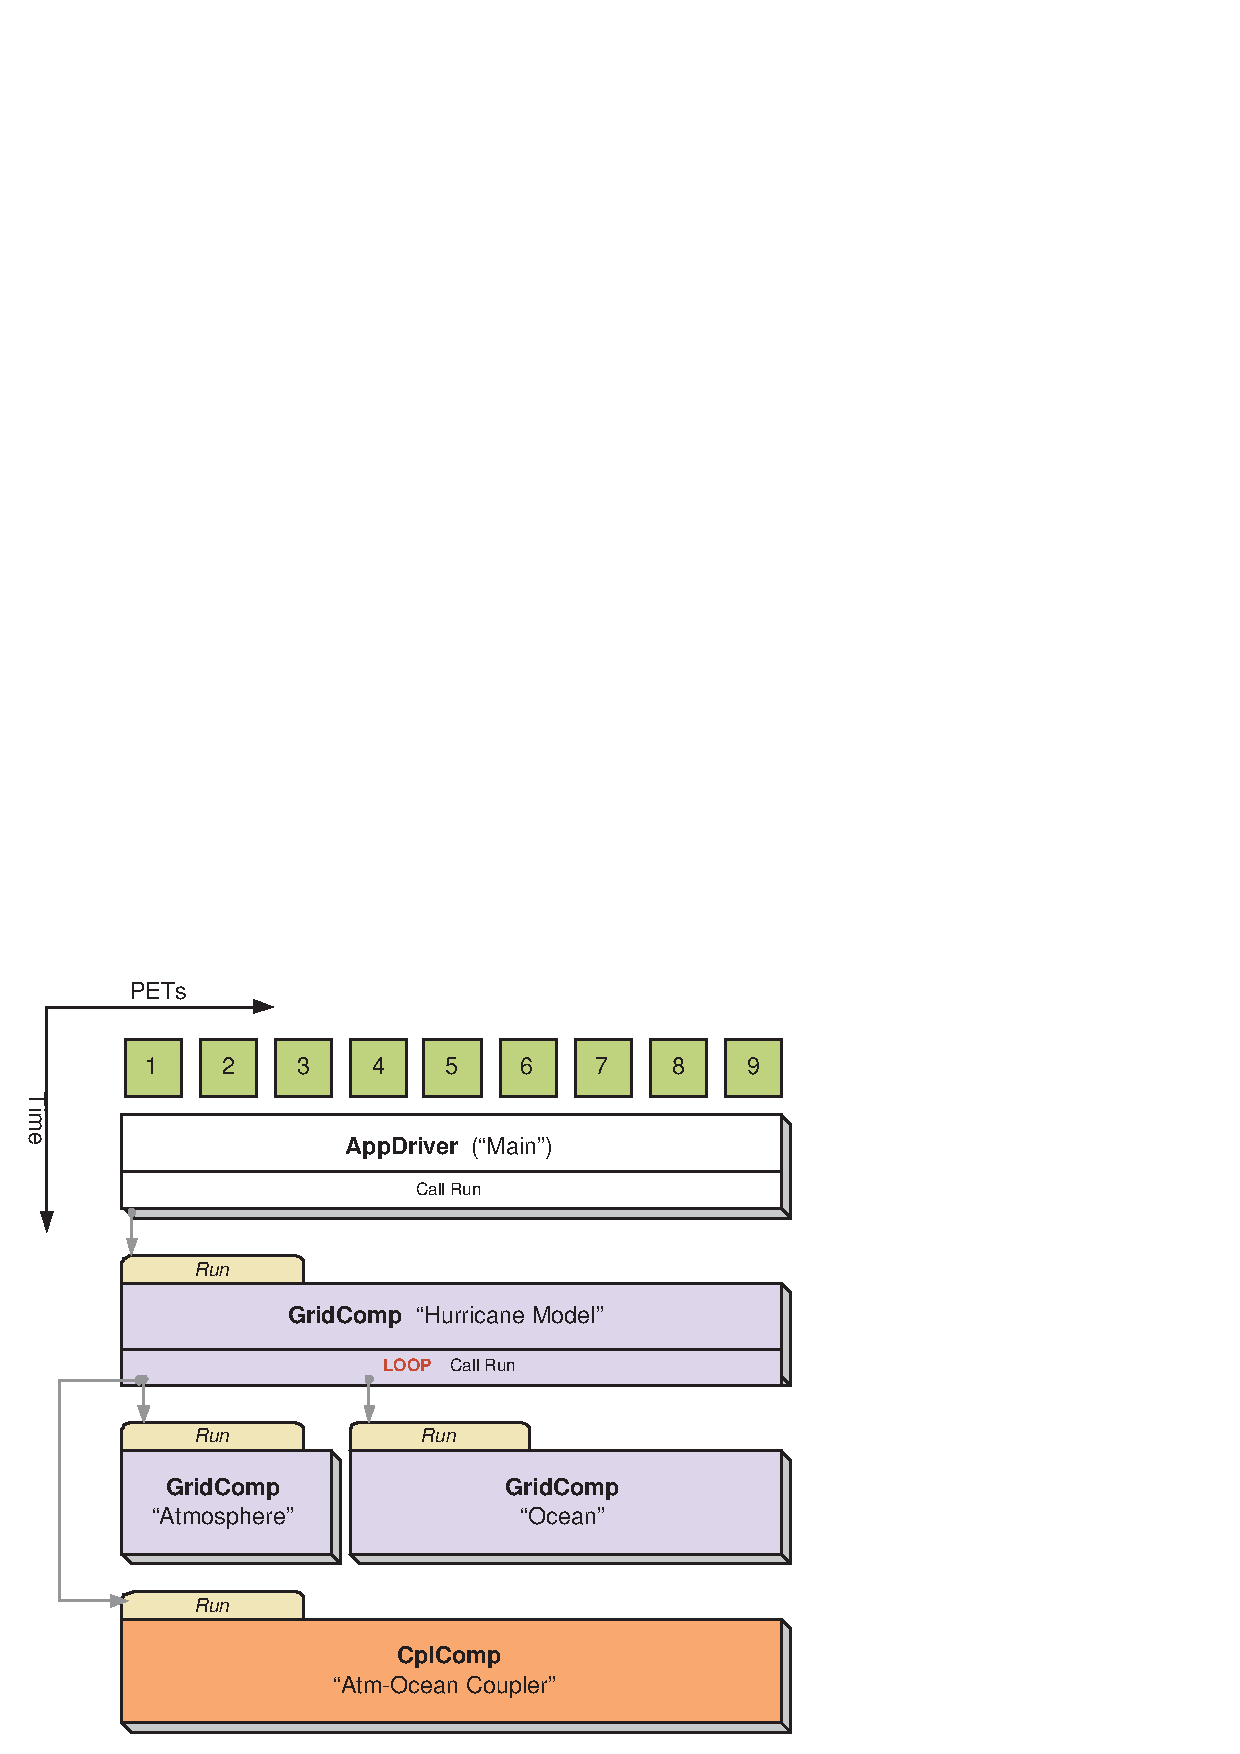
\includegraphics{ESMF_concurrent}}
\end{figure}
\end{center}

\subsection{Intra-Component Communication}
\label{sec:localcomm}

All data transfers within an ESMF application occur {\it within} a
component.  For example, a Gridded Component may contain halo updates.
Another example is that a Coupler Component may redistribute
data between two Gridded Components.  As a result,
the architecture of ESMF does not depend on any particular data
communication mechanism, and new communication schemes can be
introduced without affecting the overall structure of the application.

Since all data communication happens within a component, a Coupler
Component must be created on the union of the PETs of all
the Gridded Components that it couples.  

\subsection{Data Distribution and Scoping in Components}
\label{sec:scoping}

The scope of distributed objects is the VM of the currently 
executing Component.  For this reason, all
PETs in the current VM must make the same distributed object
creation calls.   When a Coupler Component running on a superset
of a Gridded Component's PETs needs to make communication calls
involving objects created by the Gridded Component,
an ESMF-supplied function called {\tt ESMF\_StateReconcile()} creates proxy
objects for those PETs that had no previous information about the
distributed objects.  Proxy objects contain no local data but
can be used in communication calls (such as regrid or redistribute)
to describe the remote source for data being moved to the current PET,
or to describe the remote destination for data being moved from the local PET.
Figure \ref{fig:reconcile} is a simple schematic that shows the 
sequence of events in a reconcile call.

\begin{center}
\begin{figure}
\caption{An {\tt ESMF\_StateReconcile()} call creates proxy 
objects for use in subsequent communication calls.  The reconcile 
call would normally be made during Coupler initialization.}
\label{fig:reconcile}
\scalebox{1.0}{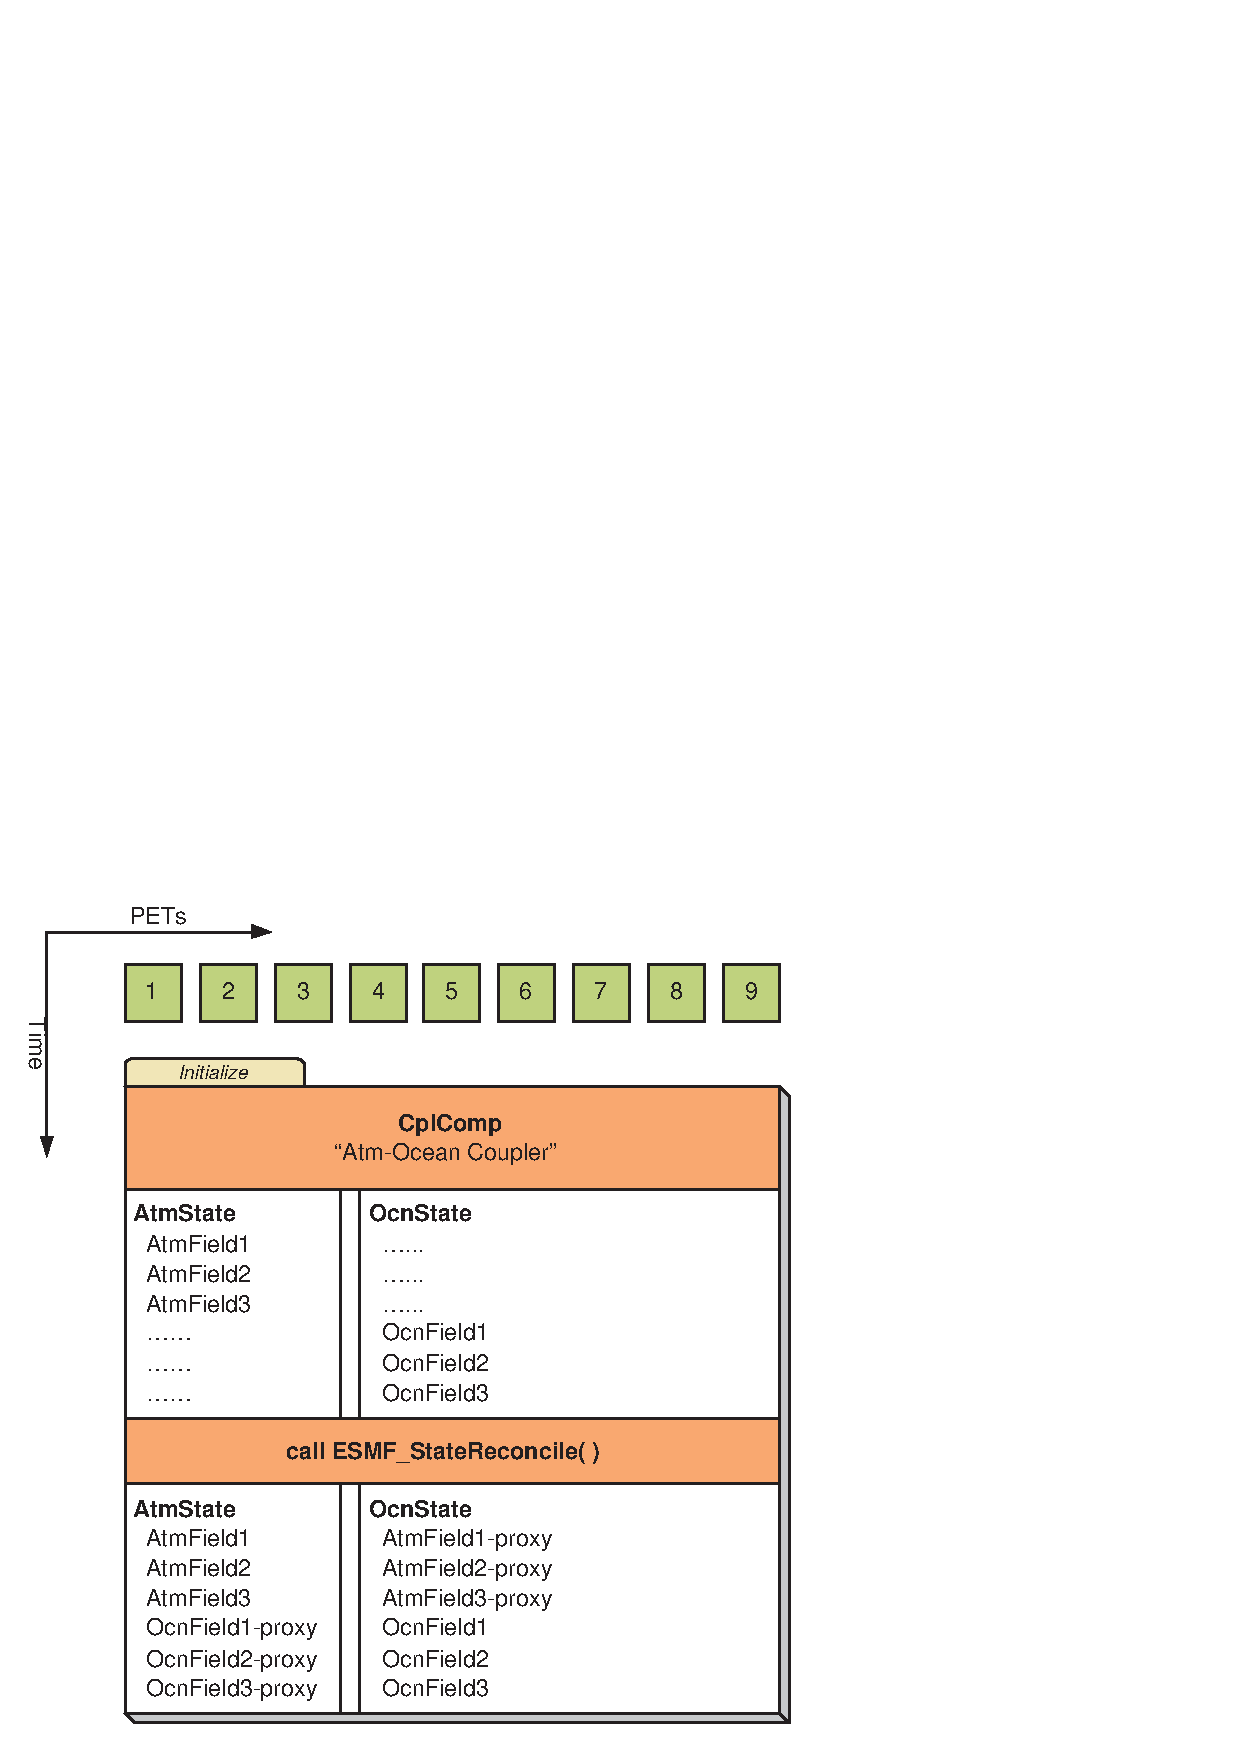
\includegraphics{ESMF_reconcile}}
\end{figure}
\end{center}

\subsection{Performance}
\label{sec:performance}

The ESMF design enables the user to configure ESMF
applications so that data is transferred directly from one component 
to another, without requiring that it be copied or sent to a different data
buffer as an interim step.  This is likely to be the most efficient way 
of performing inter-component coupling.  However, if desired, an 
application can also be configured so that data from a source component 
is sent to a distinct set of Coupler Component PETs for processing 
before being sent to its destination.

The ability to overlap computation with communication is essential for
performance.  When running with ESMF the user can initiate data 
sends during Gridded Component execution, as soon as the data is ready.
Computations can then proceed simultaneously with the data transfer.

\newpage
\subsection{Object Model}

The following is a simplified Unified Modeling Language (UML) diagram showing the relationships among
ESMF superstructure classes.  See Appendix A, {\it A Brief Introduction 
to UML}, for a translation table that lists the symbols in the diagram 
and their meaning.

\begin{center}
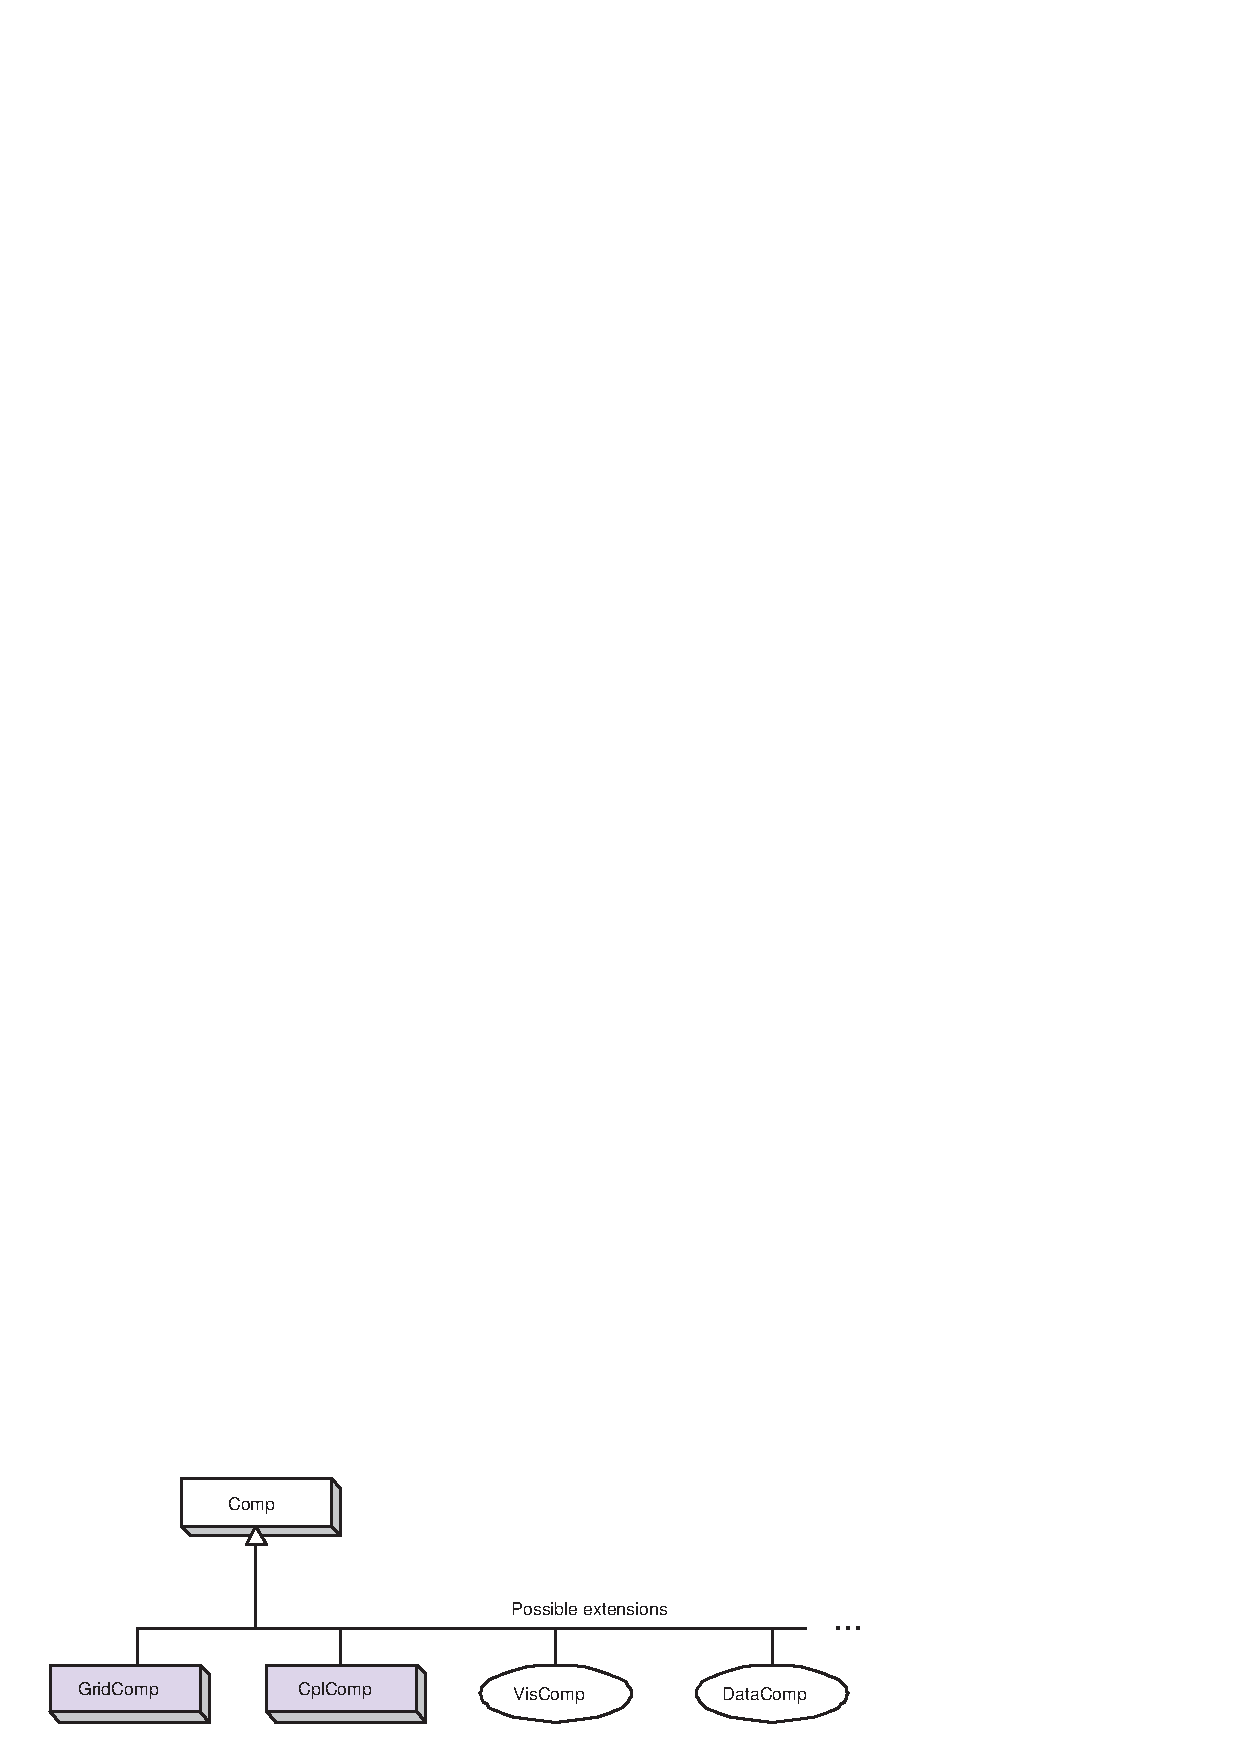
\includegraphics{Comp_obj}   
\end{center}




% $Id$
%
% Earth System Modeling Framework
% Copyright 2002-2020, University Corporation for Atmospheric Research,
% Massachusetts Institute of Technology, Geophysical Fluid Dynamics
% Laboratory, University of Michigan, National Centers for Environmental
% Prediction, Los Alamos National Laboratory, Argonne National Laboratory,
% NASA Goddard Space Flight Center.
% Licensed under the University of Illinois-NCSA License.
\bodytext{BGCOLOR=white LINK=#083194 VLINK=#21004A}
\section{Application Driver and Required ESMF Methods}
\subsection{Description}
% $Id$
%
% Earth System Modeling Framework
% Copyright 2002-2020, University Corporation for Atmospheric Research, 
% Massachusetts Institute of Technology, Geophysical Fluid Dynamics 
% Laboratory, University of Michigan, National Centers for Environmental 
% Prediction, Los Alamos National Laboratory, Argonne National Laboratory, 
% NASA Goddard Space Flight Center.
% Licensed under the University of Illinois-NCSA License.

%\subsection{Description}

Every ESMF application needs a driver code. Typically the driver layer is
implemented as the "main" of the application, although this is not strictly an
ESMF requirement. For most ESMF applications the task of the application driver
will be very generic: Initialize ESMF, create a top-level Component and call its
Initialize, Run and Finalize methods, before destroying the top-level Component
again and calling ESMF Finalize.

\begin{sloppypar}
ESMF provides a number of different application driver templates in the
{\tt \$ESMF\_DIR/src/Superstructure/AppDriver} directory. An appropriate one 
can be chosen depending on how the application is to be structured:
\end{sloppypar}

\begin{description}

\item[Sequential vs. Concurrent Execution]

In a sequential execution model, every Component executes
on all PETs, with each Component completing execution before
the next Component begins.  This has the appeal of 
simplicity of data consumption and production: when a Gridded 
Component starts, all required data is available for use, and when
a Gridded Component finishes, all data produced is ready for consumption
by the next Gridded Component.  This approach also has
the possibility of less data movement if the grid and
data decomposition is done such that each processor's memory contains
the data needed by the next Component.

In a concurrent execution model, subgroups of PETs run
Gridded Components and multiple Gridded Components are active at the 
same time.  Data exchange must be coordinated between Gridded 
Components so that data deadlock does not occur.  This strategy 
has the advantage of allowing coupling to other Gridded Components 
at any time during the computational process, including not 
having to return to the calling level of code before making 
data available.  

\item[Pairwise vs. Hub and Spoke]

Coupler Components are responsible for taking data from one
Gridded Component and putting it into the form expected by another 
Gridded Component.  This might include regridding, change of units, 
averaging, or binning.

Coupler Components can be written for {\it pairwise} data exchange: 
the Coupler Component takes data from a single Component and transforms 
it for use by another single Gridded Component.  This simplifies the 
structure of the Coupler Component code.

Couplers can also be written using a {\it hub and spoke} model where a
single Coupler accepts data from all other Components, can do data
merging or splitting, and formats data for all other Components.

Multiple Couplers, using either of the above two models or some mixture of
these approaches, are also possible.

\item[Implementation Language]

The ESMF framework currently has Fortran interfaces for all public functions. 
Some functions also have C interfaces, and the number of these is expected to 
increase over time. 


\item[Number of Executables]

The simplest way to run an application
is to run the same executable program on all PETs.  Different Components
can still be run on mutually exclusive PETs by using branching
(e.g., if this is PET 1, 2, or 3, run Component A, if it is
PET 4, 5, or 6 run Component B).  This is a {\bf SPMD} model, 
Single Program Multiple Data.  

The alternative is to start a different executable program on different
PETs.  This is a {\bf MPMD} model, Multiple Program Multiple Data.
There are complications with many job control systems on multiprocessor
machines in getting the different executables started, and getting
inter-process communications established.  ESMF currently has some
support for MPMD: different Components can run as separate executables,
but the Coupler that transfers data between the Components must still
run on the union of their PETs. This means that the Coupler Component
must be linked into all of the executables.

\end{description}




%\subsection{Constants}
%% $Id$

\subsubsection{ESMF\_END}
\label{const:endflag}

{\sf DESCRIPTION:\\}
The {\tt ESMF\_End\_Flag} determines how an ESMF application is shut down.

The type of this flag is:

{\tt type(ESMF\_End\_Flag)}

The valid values are:
\begin{description}
   \item [ESMF\_END\_ABORT] 
         Global abort of the ESMF application. There is no guarantee 
         that all PETs will shut down cleanly during an abort. However, all
         attempts are made to prevent the application from hanging and the
         LogErr of at least one PET will be completely flushed during the abort.
         This option should only be used if a condition is detected that
         prevents normal continuation or termination of the application.
         Typical conditions that warrant the use of {\tt ESMF\_END\_ABORT} 
         are those that occur on a per PET basis where other PETs may be blocked
         in communication calls, unable to reach the normal termination point.
         An aborted application returns to the parent process with a system
         dependent indication that a failure occurred during execution.
   \item [ESMF\_END\_NORMAL]
         \begin{sloppypar}
         Normal termination of the ESMF application. Wait for all PETs of the
         global VM to reach 
	{\tt ESMF\_Finalize()} before termination. This is
         the clean way of terminating an application. {\tt MPI\_Finalize()} will
         be called in case of MPI applications.
         \end{sloppypar}
   \item [ESMF\_END\_KEEPMPI]
         Same as {\tt ESMF\_END\_NORMAL} but {\tt MPI\_Finalize()} will {\em not}
         be called. It is the user code's responsibility to shut down MPI
         cleanly if necessary.
\end{description}

%\subsection{Use and Examples}
%% $Id$
%
% Earth System Modeling Framework
% Copyright 2002-2020, University Corporation for Atmospheric Research, 
% Massachusetts Institute of Technology, Geophysical Fluid Dynamics 
% Laboratory, University of Michigan, National Centers for Environmental 
% Prediction, Los Alamos National Laboratory, Argonne National Laboratory, 
% NASA Goddard Space Flight Center.
% Licensed under the University of Illinois-NCSA License.

%\subsection{Usage}

ESMF encourages application organization in which there is a single 
top-level Gridded Component.  This provides a simple, clear sequence
of operations at the highest level, and also enables the entire 
application to be treated as a sub-Component of another, larger 
application if desired.  When a simple application is organized in this fashion 
the standard AppDriver can probably be used without much modification.  

\begin{sloppypar}
Examples of program organization using the AppDriver can be found in the 
{\tt src/Superstructure/AppDriver} directory.  A set of subdirectories 
within the AppDriver directory follows the naming convention:
\end{sloppypar}
\begin{verbatim}
<seq|concur>_<pairwise|hub>_<f|c>driver_<spmd|mpmd>
\end{verbatim}

The example that is currently implemented is
{\tt seq\_pairwise\_fdriver\_spmd}, which
has sequential component execution, a pairwise coupler, a main program
in Fortran, and all processors launching the same executable.
It is also copied automatically into a top-level 
{\tt quick\_start} directory at compilation time.  

The user can copy the AppDriver files into
their own local directory. Some of the files can be used unchanged.
Others are template files which have the rough outline of the code but
need additional application-specific code added in order to perform a
meaningful function.  The {\tt README} file in the AppDriver 
subdirectory or {\tt quick\_start} directory contains instructions about 
which files to change.

Examples of concurrent component execution can be found in the
system tests that are bundled with the ESMF distribution.




%%                **** IMPORTANT NOTICE *****
% This LaTeX file has been automatically produced by ProTeX v. 1.1
% Any changes made to this file will likely be lost next time
% this file is regenerated from its source. Send questions 
% to Arlindo da Silva, dasilva@gsfc.nasa.gov
 
\setlength{\oldparskip}{\parskip}
\setlength{\parskip}{1.5ex}
\setlength{\oldparindent}{\parindent}
\setlength{\parindent}{0pt}
\setlength{\oldbaselineskip}{\baselineskip}
\setlength{\baselineskip}{11pt}
 
%--------------------- SHORT-HAND MACROS ----------------------
\def\bv{\begin{verbatim}}
\def\ev{\end{verbatim}}
\def\be{\begin{equation}}
\def\ee{\end{equation}}
\def\bea{\begin{eqnarray}}
\def\eea{\end{eqnarray}}
\def\bi{\begin{itemize}}
\def\ei{\end{itemize}}
\def\bn{\begin{enumerate}}
\def\en{\end{enumerate}}
\def\bd{\begin{description}}
\def\ed{\end{description}}
\def\({\left (}
\def\){\right )}
\def\[{\left [}
\def\]{\right ]}
\def\<{\left  \langle}
\def\>{\right \rangle}
\def\cI{{\cal I}}
\def\diag{\mathop{\rm diag}}
\def\tr{\mathop{\rm tr}}
%-------------------------------------------------------------

\markboth{Left}{Source File: AppDriver.F90,  Date: Tue May  5 21:00:19 MDT 2020
}

 
%/////////////////////////////////////////////////////////////

  \begin{verbatim}
 
  ---------------------------------------------------------------------------
  ---------------------------------------------------------------------------
   EXAMPLE:  This is an AppDriver.F90 file for a sequential ESMF application.
  ---------------------------------------------------------------------------
  ---------------------------------------------------------------------------
  
    The ChangeMe.F90 file that's included below contains a number of
    definitions that are used by the AppDriver, such as the name of the
    application's main configuration file and the name of the application's
    SetServices routine.  This file is in the same directory as the
    AppDriver.F90 file.
  ---------------------------------------------------------------------------
 
 #include "ChangeMe.F90"
 
     program ESMF_AppDriver
 #define ESMF_METHOD "program ESMF_AppDriver"
 
 #include "ESMF.h"
 
     ! ESMF module, defines all ESMF data types and procedures
     use ESMF
 
     ! Gridded Component registration routines.  Defined in "ChangeMe.F90"
     use USER_APP_Mod, only : SetServices => USER_APP_SetServices
 
     implicit none
 
  ---------------------------------------------------------------------------
    Define local variables
  ---------------------------------------------------------------------------
 
     ! Components and States
     type(ESMF_GridComp) :: compGridded
     type(ESMF_State) :: defaultstate
 
     ! Configuration information
     type(ESMF_Config) :: config
 
     ! A common Grid
     type(ESMF_Grid) :: grid
 
     ! A Clock, a Calendar, and timesteps
     type(ESMF_Clock) :: clock
     type(ESMF_TimeInterval) :: timeStep
     type(ESMF_Time) :: startTime
     type(ESMF_Time) :: stopTime
 
     ! Variables related to the Grid
     integer :: i_max, j_max
 
     ! Return codes for error checks
     integer :: rc, localrc
 
  ---------------------------------------------------------------------------
    Initialize ESMF.  Note that an output Log is created by default.
  ---------------------------------------------------------------------------
 
     call ESMF_Initialize(defaultCalKind=ESMF_CALKIND_GREGORIAN, rc=localrc)
     if (ESMF_LogFoundError(localrc, ESMF_ERR_PASSTHRU, &
         ESMF_CONTEXT, rcToReturn=rc)) &
         call ESMF_Finalize(rc=localrc, endflag=ESMF_END_ABORT)
 
     call ESMF_LogWrite("ESMF AppDriver start", ESMF_LOGMSG_INFO)
 
  ---------------------------------------------------------------------------
    Create and load a configuration file.
    The USER_CONFIG_FILE is set to sample.rc in the ChangeMe.F90 file.
    The sample.rc file is also included in the directory with the
    AppDriver.F90 file.
  ---------------------------------------------------------------------------
 
     config = ESMF_ConfigCreate(rc=localrc)
     if (ESMF_LogFoundError(localrc, ESMF_ERR_PASSTHRU, &
         ESMF_CONTEXT, rcToReturn=rc)) &
         call ESMF_Finalize(rc=localrc, endflag=ESMF_END_ABORT)
 
     call ESMF_ConfigLoadFile(config, USER_CONFIG_FILE, rc = localrc)
     if (ESMF_LogFoundError(localrc, ESMF_ERR_PASSTHRU, &
         ESMF_CONTEXT, rcToReturn=rc)) &
         call ESMF_Finalize(rc=localrc, endflag=ESMF_END_ABORT)
 
  ---------------------------------------------------------------------------
    Get configuration information.
  
    A configuration file like sample.rc might include:
    - size and coordinate information needed to create the default Grid.
    - the default start time, stop time, and running intervals
      for the main time loop.
  ---------------------------------------------------------------------------
 
     call ESMF_ConfigGetAttribute(config, i_max, label='I Counts:', &
       default=10, rc=localrc)
     if (ESMF_LogFoundError(localrc, ESMF_ERR_PASSTHRU, &
         ESMF_CONTEXT, rcToReturn=rc)) &
         call ESMF_Finalize(rc=localrc, endflag=ESMF_END_ABORT)
     call ESMF_ConfigGetAttribute(config, j_max, label='J Counts:', &
       default=40, rc=localrc)
     if (ESMF_LogFoundError(localrc, ESMF_ERR_PASSTHRU, &
         ESMF_CONTEXT, rcToReturn=rc)) &
         call ESMF_Finalize(rc=localrc, endflag=ESMF_END_ABORT)
 
  ---------------------------------------------------------------------------
    Create the top Gridded Component.
  ---------------------------------------------------------------------------
 
     compGridded = ESMF_GridCompCreate(name="ESMF Gridded Component", &
         rc=localrc)
     if (ESMF_LogFoundError(localrc, ESMF_ERR_PASSTHRU, &
         ESMF_CONTEXT, rcToReturn=rc)) &
         call ESMF_Finalize(rc=localrc, endflag=ESMF_END_ABORT)
 
     call ESMF_LogWrite("Component Create finished", ESMF_LOGMSG_INFO)
 
  ----------------------------------------------------------------------------
    Register the set services method for the top Gridded Component.
  ----------------------------------------------------------------------------
 
     call ESMF_GridCompSetServices(compGridded, userRoutine=SetServices, rc=rc)
     if (ESMF_LogFoundError(rc, msg="Registration failed", rcToReturn=rc)) &
         call ESMF_Finalize(rc=localrc, endflag=ESMF_END_ABORT)
 
  ----------------------------------------------------------------------------
    Create and initialize a Clock.
  ----------------------------------------------------------------------------
 
       call ESMF_TimeIntervalSet(timeStep, s=2, rc=localrc)
       if (ESMF_LogFoundError(localrc, ESMF_ERR_PASSTHRU, &
             ESMF_CONTEXT, rcToReturn=rc)) &
             call ESMF_Finalize(rc=localrc, endflag=ESMF_END_ABORT)
 
       call ESMF_TimeSet(startTime, yy=2004, mm=9, dd=25, rc=localrc)
       if (ESMF_LogFoundError(localrc, ESMF_ERR_PASSTHRU, &
             ESMF_CONTEXT, rcToReturn=rc)) &
             call ESMF_Finalize(rc=localrc, endflag=ESMF_END_ABORT)
 
       call ESMF_TimeSet(stopTime, yy=2004, mm=9, dd=26, rc=localrc)
       if (ESMF_LogFoundError(localrc, ESMF_ERR_PASSTHRU, &
             ESMF_CONTEXT, rcToReturn=rc)) &
             call ESMF_Finalize(rc=localrc, endflag=ESMF_END_ABORT)
 
       clock = ESMF_ClockCreate(timeStep, startTime, stopTime=stopTime, &
                 name="Application Clock", rc=localrc)
       if (ESMF_LogFoundError(localrc, ESMF_ERR_PASSTHRU, &
             ESMF_CONTEXT, rcToReturn=rc)) &
             call ESMF_Finalize(rc=localrc, endflag=ESMF_END_ABORT)
 
  ----------------------------------------------------------------------------
    Create and initialize a Grid.
  
    The default lower indices for the Grid are (/1,1/).
    The upper indices for the Grid are read in from the sample.rc file,
    where they are set to (/10,40/).  This means a Grid will be
    created with 10 grid cells in the x direction and 40 grid cells in the
    y direction.  The Grid section in the Reference Manual shows how to set
    coordinates.
  ----------------------------------------------------------------------------
 
       grid = ESMF_GridCreateNoPeriDim(maxIndex=(/i_max, j_max/), &
                              name="source grid", rc=localrc)
       if (ESMF_LogFoundError(localrc, ESMF_ERR_PASSTHRU, &
             ESMF_CONTEXT, rcToReturn=rc)) &
             call ESMF_Finalize(rc=localrc, endflag=ESMF_END_ABORT)
 
       ! Attach the grid to the Component
       call ESMF_GridCompSet(compGridded, grid=grid, rc=localrc)
       if (ESMF_LogFoundError(localrc, ESMF_ERR_PASSTHRU, &
             ESMF_CONTEXT, rcToReturn=rc)) &
             call ESMF_Finalize(rc=localrc, endflag=ESMF_END_ABORT)
 
  ----------------------------------------------------------------------------
    Create and initialize a State to use for both import and export.
    In a real code, separate import and export States would normally be
    created.
  ----------------------------------------------------------------------------
 
       defaultstate = ESMF_StateCreate(name="Default State", rc=localrc)
       if (ESMF_LogFoundError(localrc, ESMF_ERR_PASSTHRU, &
             ESMF_CONTEXT, rcToReturn=rc)) &
             call ESMF_Finalize(rc=localrc, endflag=ESMF_END_ABORT)
 
  ----------------------------------------------------------------------------
    Call the initialize, run, and finalize methods of the top component.
    When the initialize method of the top component is called, it will in
    turn call the initialize methods of all its child components, they
    will initialize their children, and so on.  The same is true of the
    run and finalize methods.
  ----------------------------------------------------------------------------
 
       call ESMF_GridCompInitialize(compGridded, importState=defaultstate, &
         exportState=defaultstate, clock=clock, rc=localrc)
       if (ESMF_LogFoundError(rc, msg="Initialize failed", rcToReturn=rc)) &
           call ESMF_Finalize(rc=localrc, endflag=ESMF_END_ABORT)
 
       call ESMF_GridCompRun(compGridded, importState=defaultstate, &
         exportState=defaultstate, clock=clock, rc=localrc)
       if (ESMF_LogFoundError(rc, msg="Run failed", rcToReturn=rc)) &
           call ESMF_Finalize(rc=localrc, endflag=ESMF_END_ABORT)
 
       call ESMF_GridCompFinalize(compGridded, importState=defaultstate, &
         exportState=defaultstate, clock=clock, rc=localrc)
       if (ESMF_LogFoundError(rc, msg="Finalize failed", rcToReturn=rc)) &
           call ESMF_Finalize(rc=localrc, endflag=ESMF_END_ABORT)
 
 
  ----------------------------------------------------------------------------
    Destroy objects.
  ----------------------------------------------------------------------------
 
       call ESMF_ClockDestroy(clock, rc=localrc)
       if (ESMF_LogFoundError(localrc, ESMF_ERR_PASSTHRU, &
         ESMF_CONTEXT, rcToReturn=rc)) &
         call ESMF_Finalize(rc=localrc, endflag=ESMF_END_ABORT)
 
       call ESMF_StateDestroy(defaultstate, rc=localrc)
       if (ESMF_LogFoundError(localrc, ESMF_ERR_PASSTHRU, &
         ESMF_CONTEXT, rcToReturn=rc)) &
         call ESMF_Finalize(rc=localrc, endflag=ESMF_END_ABORT)
 
       call ESMF_GridCompDestroy(compGridded, rc=localrc)
       if (ESMF_LogFoundError(localrc, ESMF_ERR_PASSTHRU, &
         ESMF_CONTEXT, rcToReturn=rc)) &
         call ESMF_Finalize(rc=localrc, endflag=ESMF_END_ABORT)
 
  ----------------------------------------------------------------------------
    Finalize and clean up.
  ----------------------------------------------------------------------------
 
     call ESMF_Finalize()
 
     end program ESMF_AppDriver
 
  \end{verbatim}
%...............................................................
\setlength{\parskip}{\oldparskip}
\setlength{\parindent}{\oldparindent}
\setlength{\baselineskip}{\oldbaselineskip}

%\subsection{Restrictions and Future Work}
%#ifdef STANDALONE
%% $Id$
%
% Earth System Modeling Framework
% Copyright 2002-2020, University Corporation for Atmospheric Research, 
% Massachusetts Institute of Technology, Geophysical Fluid Dynamics 
% Laboratory, University of Michigan, National Centers for Environmental 
% Prediction, Los Alamos National Laboratory, Argonne National Laboratory, 
% NASA Goddard Space Flight Center.
% Licensed under the University of Illinois-NCSA License.

%\subsubsection{Restrictions and Future Work}

\begin{enumerate}

\item {\bf MPMD not supported.}  Only single executable applications 
are supported at this time. 

\end{enumerate}

%#elif defined(1)
%% $Id$
%
% Earth System Modeling Framework
% Copyright 2002-2020, University Corporation for Atmospheric Research, 
% Massachusetts Institute of Technology, Geophysical Fluid Dynamics 
% Laboratory, University of Michigan, National Centers for Environmental 
% Prediction, Los Alamos National Laboratory, Argonne National Laboratory, 
% NASA Goddard Space Flight Center.
% Licensed under the University of Illinois-NCSA License.

%\subsubsection{Restrictions and Future Work}

\begin{enumerate}

\item {\bf MPMD not supported.}  Only single executable applications 
are supported at this time. 

\end{enumerate}

%#endif
\subsection{Required ESMF Methods}
% $Id$
%
% Earth System Modeling Framework
% Copyright 2002-2020, University Corporation for Atmospheric Research, 
% Massachusetts Institute of Technology, Geophysical Fluid Dynamics 
% Laboratory, University of Michigan, National Centers for Environmental 
% Prediction, Los Alamos National Laboratory, Argonne National Laboratory, 
% NASA Goddard Space Flight Center.
% Licensed under the University of Illinois-NCSA License.

There are a few methods that every ESMF application must contain. First,
{\tt ESMC\_Initialize()} and {\tt ESMC\_Finalize()} are in complete analogy 
to {\tt MPI\_Init()} and {\tt MPI\_Finalize()} known from MPI. All ESMF
programs, serial or parallel, must initialize the ESMF system at the beginning,
and finalize it at the end of execution. The behavior of calling any
ESMF method before {\tt ESMC\_Initialize()}, or after {\tt ESMC\_Finalize()}
is undefined.

Second, every ESMF Component that is accessed by an ESMF application requires
that its set services routine is called through
{\tt ESMC\_<Grid/Cpl>CompSetServices()}. The Component must implement
one public entry point, its set services routine, that can be called
through the {\tt ESMC\_<Grid/Cpl>CompSetServices()} library routine. The
Component set services routine is responsible for setting entry points
for the standard ESMF Component methods Initialize, Run, and Finalize.

Finally, the Component can optionally call {\tt ESMC\_<Grid/Cpl>CompSetVM()}
{\em before} calling
{\tt ESMC\_<Grid/Cpl>CompSetServices()}. Similar to 
{\tt ESMC\_<Grid/Cpl>CompSetServices()}, the 
\newline
{\tt ESMC\_<Grid/Cpl>CompSetVM()}
call requires a public entry point into the Component. It allows the Component
to adjust certain aspects of its execution environment, i.e. its own VM, before
it is started up.

The following sections discuss the above mentioned aspects in more detail.

%%                **** IMPORTANT NOTICE *****
% This LaTeX file has been automatically produced by ProTeX v. 1.1
% Any changes made to this file will likely be lost next time
% this file is regenerated from its source. Send questions 
% to Arlindo da Silva, dasilva@gsfc.nasa.gov
 
\setlength{\oldparskip}{\parskip}
\setlength{\parskip}{1.5ex}
\setlength{\oldparindent}{\parindent}
\setlength{\parindent}{0pt}
\setlength{\oldbaselineskip}{\baselineskip}
\setlength{\baselineskip}{11pt}
 
%--------------------- SHORT-HAND MACROS ----------------------
\def\bv{\begin{verbatim}}
\def\ev{\end{verbatim}}
\def\be{\begin{equation}}
\def\ee{\end{equation}}
\def\bea{\begin{eqnarray}}
\def\eea{\end{eqnarray}}
\def\bi{\begin{itemize}}
\def\ei{\end{itemize}}
\def\bn{\begin{enumerate}}
\def\en{\end{enumerate}}
\def\bd{\begin{description}}
\def\ed{\end{description}}
\def\({\left (}
\def\){\right )}
\def\[{\left [}
\def\]{\right ]}
\def\<{\left  \langle}
\def\>{\right \rangle}
\def\cI{{\cal I}}
\def\diag{\mathop{\rm diag}}
\def\tr{\mathop{\rm tr}}
%-------------------------------------------------------------

\markboth{Left}{Source File: ESMF\_Init.F90,  Date: Tue May  5 21:00:19 MDT 2020
}

 
%/////////////////////////////////////////////////////////////

  
%/////////////////////////////////////////////////////////////
 
\mbox{}\hrulefill\ 
 
\subsubsection [ESMF\_Initialize] {ESMF\_Initialize - Initialize ESMF}


  
\bigskip{\sf INTERFACE:}
\begin{verbatim}       subroutine ESMF_Initialize(defaultConfigFileName, defaultCalKind, &
         defaultLogFileName, logappendflag, logkindflag, mpiCommunicator,  &
         ioUnitLBound, ioUnitUBound, vm, rc)\end{verbatim}{\em ARGUMENTS:}
\begin{verbatim} -- The following arguments require argument keyword syntax (e.g. rc=rc). --
       character(len=*),        intent(in),  optional :: defaultConfigFileName
       type(ESMF_CalKind_Flag), intent(in),  optional :: defaultCalKind
       character(len=*),        intent(in),  optional :: defaultLogFileName
       logical,                 intent(in),  optional :: logappendflag
       type(ESMF_LogKind_Flag), intent(in),  optional :: logkindflag
       integer,                 intent(in),  optional :: mpiCommunicator
       integer,                 intent(in),  optional :: ioUnitLBound
       integer,                 intent(in),  optional :: ioUnitUBound
       type(ESMF_VM),           intent(out), optional :: vm
       integer,                 intent(out), optional :: rc
 \end{verbatim}
{\sf STATUS:}
   \begin{itemize}
   \item\apiStatusCompatibleVersion{5.2.0r}
   \item\apiStatusModifiedSinceVersion{5.2.0r}
   \begin{description}
   \item[7.0.0] Added argument {\tt logappendflag} to allow specifying that the existing
                log files will be overwritten.\newline
   \end{description}
   \end{itemize}
  
{\sf DESCRIPTION:\\ }


       This method must be called once on each PET before
       any other ESMF methods are used.  The method contains a
       barrier before returning, ensuring that all processes
       made it successfully through initialization.
  
       Typically {\tt ESMF\_Initialize()} will call {\tt MPI\_Init()} 
       internally unless MPI has been initialized by the user code before
       initializing the framework. If the MPI initialization is left to
       {\tt ESMF\_Initialize()} it inherits all of the MPI implementation 
       dependent limitations of what may or may not be done before 
       {\tt MPI\_Init()}. For instance, it is unsafe for some MPI
       implementations, such as MPICH, to do I/O before the MPI environment
       is initialized. Please consult the documentation of your MPI
       implementation for details.
  
       Note that when using MPICH as the MPI library, ESMF needs to use
       the application command line arguments for {\tt MPI\_Init()}. However,
       ESMF acquires these arguments internally and the user does not need
       to worry about providing them. Also, note that ESMF does not alter
       the command line arguments, so that if the user obtains them they will
       be as specified on the command line (including those which MPICH would
       normally strip out).
  
       {\tt ESMF\_Initialize()} supports running ESMF inside a user MPI program.
       Details of this feature are discussed under the VM example 
       \ref{vm_inside_user_mpi}. It is not necessary that all MPI ranks are
       handed to ESMF. Section \ref{vm_nesting_esmf} shows how an MPI
       communicator can be used to execute ESMF on a subset of MPI ranks.
       Finally {\tt ESMF\_Initialize()} supports running multiple concurrent
       instances of ESMF under the same user MPI program. This feature is
       discussed under \ref{vm_multi_instance_esmf}.
  
       By default, {\tt ESMF\_Initialize()} will open multiple error log files,
       one per processor.  This is very useful for debugging purpose.  However,
       when running the application on a large number of processors, opening a
       large number of log files and writing log messages from all the processors
       could become a performance bottleneck.  Therefore, it is recommended
       to turn the Error Log feature off in these situations by setting
       {\tt logkindflag} to ESMF\_LOGKIND\_NONE.
  
       When integrating ESMF with applications where Fortran unit number conflicts
       exist, the optional {\tt ioUnitLBound} and {\tt ioUnitUBound} arguments may be
       used to specify an alternate unit number range.  See section \ref{fio:unitnumbers}
       for more information on how ESMF uses Fortran unit numbers.
  
       Before exiting the application the user must call {\tt ESMF\_Finalize()}
       to release resources and clean up ESMF gracefully.
  
       The arguments are:
       \begin{description}
       \item [{[defaultConfigFilename]}]
             Name of the default configuration file for the entire application.
       \item [{[defaultCalKind]}]
             Sets the default calendar to be used by ESMF Time Manager.
             See section \ref{const:calkindflag} for a list of valid options.
             If not specified, defaults to {\tt ESMF\_CALKIND\_NOCALENDAR}.
       \item [{[defaultLogFileName]}]
             Name of the default log file for warning and error messages.
             If not specified, defaults to {\tt ESMF\_ErrorLog}.
       \item [{[logappendflag]}]
             If the default log file already exists, a value of {\tt .false.}
             will set the file position to the beginning of the file.  A value
             of {\tt .true.} sets the position to the end of the file.
             If not specified, defaults to {\tt .true.}.
       \item [{[logkindflag]}]
             Sets the default Log Type to be used by ESMF Log Manager.
             See section \ref{const:logkindflag} for a list of valid options.
             If not specified, defaults to {\tt ESMF\_LOGKIND\_MULTI}.
       \item [{[mpiCommunicator]}]
             MPI communicator defining the group of processes on which the
             ESMF application is running.
             See section \ref{vm_nesting_esmf} and \ref{vm_multi_instance_esmf}
             for details.
             If not specified, defaults to {\tt MPI\_COMM\_WORLD}.
       \item [{[ioUnitLBound]}]
             Lower bound for Fortran unit numbers used within the ESMF library.
             Fortran units are primarily used for log files.  Legal unit numbers
             are positive integers.  A value higher than 10 is recommended
             in order to avoid the compiler-specific
             reservations which are typically found on the first few units.
             If not specified, defaults to {\tt ESMF\_LOG\_FORT\_UNIT\_NUMBER},
             which is distributed with a value of 50.
       \item [{[ioUnitUBound]}]
             Upper bound for Fortran unit numbers used within the ESMF library.
             Must be set to a value at least 5 units higher than {\tt ioUnitLBound}.
             If not specified, defaults to {\tt ESMF\_LOG\_UPPER}, which is
             distributed with a value of 99.
       \item [{[vm]}]
             Returns the global {\tt ESMF\_VM} that was created 
             during initialization.
       \item [{[rc]}]
             Return code; equals {\tt ESMF\_SUCCESS} if there are no errors.
  
       \end{description} 
%/////////////////////////////////////////////////////////////
 
\mbox{}\hrulefill\ 
 
\subsubsection [ESMF\_IsInitialized] {ESMF\_IsInitialized - Query Initialized status of ESMF}


  
\bigskip{\sf INTERFACE:}
\begin{verbatim}     function ESMF_IsInitialized(rc)\end{verbatim}{\em RETURN VALUE:}
\begin{verbatim}       logical :: ESMF_IsInitialized\end{verbatim}{\em ARGUMENTS:}
\begin{verbatim} -- The following arguments require argument keyword syntax (e.g. rc=rc). --
       integer,                 intent(out), optional :: rc
 \end{verbatim}
{\sf DESCRIPTION:\\ }


       Returns {\tt .true.} if the framework has been initialized. This means 
       that {\tt ESMF\_Initialize()} has been called. Otherwise returns
       {\tt .false.}. If an error occurs, i.e. {\tt rc /= ESMF\_SUCCESS} is 
       returned, the return value of the function will also be {\tt .false.}.
  
       The arguments are:
       \begin{description}
       \item [{[rc]}]
             Return code; equals {\tt ESMF\_SUCCESS} if there are no errors.
  
       \end{description} 
%/////////////////////////////////////////////////////////////
 
\mbox{}\hrulefill\ 
 
\subsubsection [ESMF\_IsFinalized] {ESMF\_IsFinalized - Query Finalized status of ESMF}


  
\bigskip{\sf INTERFACE:}
\begin{verbatim}     function ESMF_IsFinalized(rc)\end{verbatim}{\em RETURN VALUE:}
\begin{verbatim}       logical :: ESMF_IsFinalized\end{verbatim}{\em ARGUMENTS:}
\begin{verbatim} -- The following arguments require argument keyword syntax (e.g. rc=rc). --
       integer,                 intent(out), optional :: rc
 \end{verbatim}
{\sf DESCRIPTION:\\ }


       Returns {\tt .true.} if the framework has been finalized. This means 
       that {\tt ESMF\_Finalize()} has been called. Otherwise returns
       {\tt .false.}. If an error occurs, i.e. {\tt rc /= ESMF\_SUCCESS} is 
       returned, the return value of the function will also be {\tt .false.}.
  
       The arguments are:
       \begin{description}
       \item [{[rc]}]
             Return code; equals {\tt ESMF\_SUCCESS} if there are no errors.
  
       \end{description} 
%/////////////////////////////////////////////////////////////
 
\mbox{}\hrulefill\ 
 
\subsubsection [ESMF\_Finalize] {ESMF\_Finalize - Clean up and shut down ESMF}


  
\bigskip{\sf INTERFACE:}
\begin{verbatim}       subroutine ESMF_Finalize(endflag, rc)\end{verbatim}{\em ARGUMENTS:}
\begin{verbatim} -- The following arguments require argument keyword syntax (e.g. rc=rc). --
       type(ESMF_End_Flag), intent(in), optional  :: endflag
       integer,             intent(out), optional :: rc
 \end{verbatim}
{\sf STATUS:}
   \begin{itemize}
   \item\apiStatusCompatibleVersion{5.2.0r}
   \end{itemize}
  
{\sf DESCRIPTION:\\ }


       This must be called once on each PET before the application exits
       to allow ESMF to flush buffers, close open connections, and 
       release internal resources cleanly. The optional argument 
       {\tt endflag} may be used to indicate the mode of termination.  
       Note that this call must be issued only once per PET with 
       {\tt endflag=ESMF\_END\_NORMAL}, and that this call may not be followed
       by {\tt ESMF\_Initialize()}.  This last restriction means that it is not
       possible to restart ESMF within the same execution.
  
       The arguments are:
       \begin{description}
       \item [{[endflag]}]
             Specify mode of termination. The default is {\tt ESMF\_END\_NORMAL}
             which waits for all PETs of the global VM to reach 
             {\tt ESMF\_Finalize()} before termination. See section 
             \ref{const:endflag} for a complete list and description of
             valid flags.
       \item [{[rc]}]
             Return code; equals {\tt ESMF\_SUCCESS} if there are no errors.
       \end{description}
  
%...............................................................
\setlength{\parskip}{\oldparskip}
\setlength{\parindent}{\oldparindent}
\setlength{\baselineskip}{\oldbaselineskip}

%                **** IMPORTANT NOTICE *****
% This LaTeX file has been automatically produced by ProTeX v. 1.1
% Any changes made to this file will likely be lost next time
% this file is regenerated from its source. Send questions 
% to Arlindo da Silva, dasilva@gsfc.nasa.gov
 
\setlength{\oldparskip}{\parskip}
\setlength{\parskip}{1.5ex}
\setlength{\oldparindent}{\parindent}
\setlength{\parindent}{0pt}
\setlength{\oldbaselineskip}{\baselineskip}
\setlength{\baselineskip}{11pt}
 
%--------------------- SHORT-HAND MACROS ----------------------
\def\bv{\begin{verbatim}}
\def\ev{\end{verbatim}}
\def\be{\begin{equation}}
\def\ee{\end{equation}}
\def\bea{\begin{eqnarray}}
\def\eea{\end{eqnarray}}
\def\bi{\begin{itemize}}
\def\ei{\end{itemize}}
\def\bn{\begin{enumerate}}
\def\en{\end{enumerate}}
\def\bd{\begin{description}}
\def\ed{\end{description}}
\def\({\left (}
\def\){\right )}
\def\[{\left [}
\def\]{\right ]}
\def\<{\left  \langle}
\def\>{\right \rangle}
\def\cI{{\cal I}}
\def\diag{\mathop{\rm diag}}
\def\tr{\mathop{\rm tr}}
%-------------------------------------------------------------

\markboth{Left}{Source File: ESMC\_Init.h,  Date: Tue May  5 21:00:19 MDT 2020
}

 
%/////////////////////////////////////////////////////////////
\subsubsection [ESMC\_Initialize] {ESMC\_Initialize - Initialize ESMF}


  
\bigskip{\sf INTERFACE:}
\begin{verbatim}   int ESMC_Initialize(
     int *rc,        // return code
     ...);           // optional arguments (see below)
 \end{verbatim}{\em RETURN VALUE:}
\begin{verbatim}    Return code; equals ESMF_SUCCESS if there are no errors.\end{verbatim}
{\sf DESCRIPTION:\\ }


    Initialize the ESMF.  This method must be called before
    any other ESMF methods are used.  The method contains a
    barrier before returning, ensuring that all processes
    made it successfully through initialization.
  
    Typically {\tt ESMC\_Initialize()} will call {\tt MPI\_Init()} 
    internally unless MPI has been initialized by the user code before
    initializing the framework. If the MPI initialization is left to
    {\tt ESMC\_Initialize()} it inherits all of the MPI implementation 
    dependent limitations of what may or may not be done before 
    {\tt MPI\_Init()}. For instance, it is unsafe for some MPI implementations,
    such as MPICH, to do I/O before the MPI environment is initialized. Please
    consult the documentation of your MPI implementation for details.
  
    Optional arguments are recognised.  To indicate the end of the optional
    argument list, {\tt ESMC\_ArgLast} must be used.  A minimal call to
    {\tt ESMC\_Initialize()} would be:
   \begin{verbatim}
      ESMC_Initialize (NULL, ESMC_ArgLast);\end{verbatim}
    The optional arguments are specified using the {\tt ESMC\_InitArg} macros.
    For example, to turn off logging so that no log files would be created, the
    {\tt ESMC\_Initialize()} call would be coded as:
   \begin{verbatim}
      ESMC_Initialize (&rc,
        ESMC_InitArgLogKindFlag(ESMC_LOGKIND_NONE),
        ESMC_ArgLast);\end{verbatim}
    Before exiting the application the user must call {\tt ESMC\_Finalize()}
    to release resources and clean up the ESMF gracefully.
  
    The arguments are:
    \begin{description}
    \item [{[rc]}]
      Return code; equals {\tt ESMF\_SUCCESS} if there are no errors.
      {\tt NULL} may be passed when the return code is not desired.
    \item [{[ESMC\_InitArgDefaultCalKind(ARG)]}]
      Macro specifying the default calendar kind for the entire
      application.  Valid values for {\tt ARG} are documented in section
      \ref{const:calkindflag_c}.
      If not specified, defaults to {\tt ESMC\_CALKIND\_NOCALENDAR}.
    \item [{[ESMC\_InitArgDefaultConfigFilename(ARG)]}]
      Macro specifying the name of the default configuration file for the
      Config class.  If not specified, no default file is used.
    \item [{[ESMC\_InitArgLogFilename(ARG)]}]
      Macro specifying the name used as part of the default log file name for
      the default log.  If not specified, defaults to {\tt ESMF\_LogFile}.
    \item [{[ESMC\_InitArgLogKindFlag(ARG)]}]
      Macro specifying the default Log kind to be used by ESMF Log Manager.
      Valid values for {\tt ARG} are  documented in section
      \ref{const:clogkindflag}.
      If not specified, defaults to {\tt ESMC\_LOGKIND\_MULTI}.
    \item [ESMC\_ArgLast]
      Macro indicating the end of the optional argument list.  This must be
      provided even when there are no optional arguments.
    \end{description} 
%/////////////////////////////////////////////////////////////
 
\mbox{}\hrulefill\ 
 
\subsubsection [ESMC\_Finalize] {ESMC\_Finalize - Finalize the ESMF Framework}


  
\bigskip{\sf INTERFACE:}
\begin{verbatim}   int ESMC_Finalize(void);
 \end{verbatim}{\em RETURN VALUE:}
\begin{verbatim}    Return code; equals ESMF_SUCCESS if there are no errors.\end{verbatim}
{\sf DESCRIPTION:\\ }


   This must be called once on each PET before the application exits to
   allow ESMF to flush buffers, close open connections, and release
   internal resources cleanly.
%...............................................................
\setlength{\parskip}{\oldparskip}
\setlength{\parindent}{\oldparindent}
\setlength{\baselineskip}{\oldbaselineskip}

%%%%%%% end class sections %%%%%%%%
% $Id$
%
% Earth System Modeling Framework
% Copyright 2002-2020, University Corporation for Atmospheric Research,
% Massachusetts Institute of Technology, Geophysical Fluid Dynamics
% Laboratory, University of Michigan, National Centers for Environmental
% Prediction, Los Alamos National Laboratory, Argonne National Laboratory,
% NASA Goddard Space Flight Center.
% Licensed under the University of Illinois-NCSA License.
\bodytext{BGCOLOR=white LINK=#083194 VLINK=#21004A}
%%%%%%%%%%%%% Gridded Component Class %%%%%%%%%
\section{GridComp Class}
\subsection{Description}
% $Id$
%
% Earth System Modeling Framework
% Copyright 2002-2020, University Corporation for Atmospheric Research, 
% Massachusetts Institute of Technology, Geophysical Fluid Dynamics 
% Laboratory, University of Michigan, National Centers for Environmental 
% Prediction, Los Alamos National Laboratory, Argonne National Laboratory, 
% NASA Goddard Space Flight Center.
% Licensed under the University of Illinois-NCSA License.

%TODO: This file started as an exact copy of the Fortran version of this file.
%TODO: It was changed to the C version by ESMF->ESMC subsitution.
%TODO: We should check into using latex command defintion to generate this
%TODO: sort of language specific document from a single generic document.

%\subsection{Description}
\label{sec:GridComp}

In Earth system modeling, the most natural way to think about an ESMF 
Gridded Component, or {\tt ESMC\_GridComp}, is as a piece of code 
representing a particular physical domain, such as an atmospheric 
model or an ocean model.  Gridded Components may also represent individual
processes, such as radiation or chemistry.  It's up to the application
writer to decide how deeply to ``componentize.''

Earth system software components tend to share a number of basic 
features.  Most ingest and produce a variety of physical fields, refer to 
a (possibly noncontiguous) spatial region and a grid that is 
partitioned across a set of computational resources, and require 
a clock for things like stepping a governing set of PDEs forward in time.  
Most can also be divided into distinct initialize, run, and finalize 
computational phases.  These common characteristics are used 
within ESMF to define a Gridded Component data structure that 
is tailored for Earth system modeling and yet is still flexible
enough to represent a variety of domains.

A well designed Gridded Component does not store information 
internally about how it couples to other Gridded Components.  That
allows it to be used in different contexts without changes to source
code.  The idea here is to avoid situations in which slightly
different versions of the same model source are maintained for use in 
different contexts - standalone vs. coupled versions, for example.
Data is passed in and out of Gridded Components using an ESMF State,
this is described in Section~\ref{sec:State}.

An ESMF Gridded Component has two parts, one which is user-written
and another which is part of the framework.  The user-written
part is software that represents a physical domain or performs some
other computational function.  It forms the body of the Gridded 
Component.  It may be a piece of legacy code, or it may be developed 
expressly for use with ESMF.  It must contain routines with
standard ESMF interfaces that can be called to initialize, run, and
finalize the Gridded Component.  These routines can have separate 
callable phases, such as distinct first and second initialization steps.

ESMF provides the Gridded Component derived type, 
{\tt ESMC\_GridComp}.  An {\tt ESMC\_GridComp} must be created 
for every portion of the application that will be represented 
as a separate component.  For example, in a climate model, there may 
be Gridded Components representing the land, ocean, sea ice, and 
atmosphere.  If the application contains an ensemble of identical 
Gridded Components, every one has its own associated {\tt ESMC\_GridComp}.
Each Gridded Component has its own name and is allocated
a set of computational resources, in the form of an ESMF Virtual
Machine, or {\tt VM}.

The user-written part of a Gridded Component is associated with an
{\tt ESMC\_GridComp} derived type through a routine called 
{\tt ESMC\_SetServices()}.
This is a routine that the user must write, and declare public.
Inside the SetServices routine the user must call  
{\tt ESMC\_SetEntryPoint()} methods that associate a standard ESMF 
operation with the name of the corresponding Fortran subroutine 
in their user code.

%\subsection{GridComp Options}
%#ifdef STANDALONE
%\input{GridComp_options}
%#elif defined(1)
%\input{../Superstructure/Component/doc/GridComp_options}
%#endif
%\subsection{Use and Examples}
%% $Id$
%
% Earth System Modeling Framework
% Copyright 2002-2020, University Corporation for Atmospheric Research, 
% Massachusetts Institute of Technology, Geophysical Fluid Dynamics 
% Laboratory, University of Michigan, National Centers for Environmental 
% Prediction, Los Alamos National Laboratory, Argonne National Laboratory, 
% NASA Goddard Space Flight Center.
% Licensed under the University of Illinois-NCSA License.

%\subsection{Use and Examples}

A Gridded Component is a computational entity which consumes and produces data. It uses a State object to exchange data between itself and other Components. It uses a Clock object to manage time, and a VM to describe its own and its child components' computational resources.

This section shows how to create Gridded Components.  For demonstrations
of the use of Gridded Components, see the system tests that are bundled with the ESMF software
distribution.  These can be found in the directory {\tt esmf/src/system\_tests}.




%%                **** IMPORTANT NOTICE *****
% This LaTeX file has been automatically produced by ProTeX v. 1.1
% Any changes made to this file will likely be lost next time
% this file is regenerated from its source. Send questions 
% to Arlindo da Silva, dasilva@gsfc.nasa.gov
 
\setlength{\oldparskip}{\parskip}
\setlength{\parskip}{1.5ex}
\setlength{\oldparindent}{\parindent}
\setlength{\parindent}{0pt}
\setlength{\oldbaselineskip}{\baselineskip}
\setlength{\baselineskip}{11pt}
 
%--------------------- SHORT-HAND MACROS ----------------------
\def\bv{\begin{verbatim}}
\def\ev{\end{verbatim}}
\def\be{\begin{equation}}
\def\ee{\end{equation}}
\def\bea{\begin{eqnarray}}
\def\eea{\end{eqnarray}}
\def\bi{\begin{itemize}}
\def\ei{\end{itemize}}
\def\bn{\begin{enumerate}}
\def\en{\end{enumerate}}
\def\bd{\begin{description}}
\def\ed{\end{description}}
\def\({\left (}
\def\){\right )}
\def\[{\left [}
\def\]{\right ]}
\def\<{\left  \langle}
\def\>{\right \rangle}
\def\cI{{\cal I}}
\def\diag{\mathop{\rm diag}}
\def\tr{\mathop{\rm tr}}
%-------------------------------------------------------------

\markboth{Left}{Source File: ESMF\_GCompEx.F90,  Date: Tue May  5 21:00:11 MDT 2020
}

 
%/////////////////////////////////////////////////////////////

  \subsubsection{Implement a user-code {\tt SetServices} routine}
   
   \label{sec:GridSetServ}
  
   Every {\tt ESMF\_GridComp} is required to provide and document
   a public set services routine.  It can have any name, but must
   follow the declaration below: a subroutine which takes an
   {\tt ESMF\_GridComp} as the first argument, and
   an integer return code as the second.
   Both arguments are required and must {\em not} be declared as 
   {\tt optional}. If an intent is specified in the interface it must be 
   {\tt intent(inout)} for the first and {\tt intent(out)} for the 
   second argument.
  
   The set services routine must call the ESMF method 
   {\tt ESMF\_GridCompSetEntryPoint()} to
   register with the framework what user-code subroutines should be called 
   to initialize, run, and finalize the component.  There are
   additional routines which can be registered as well, for checkpoint
   and restart functions.
  
   Note that the actual subroutines being registered do not have to be
   public to this module; only the set services routine itself must
   be available to be used by other code. 
%/////////////////////////////////////////////////////////////

 \begin{verbatim}
    ! Example Gridded Component
    module ESMF_GriddedCompEx
    
    ! ESMF Framework module
    use ESMF
    implicit none
    public GComp_SetServices
    public GComp_SetVM

    contains

    subroutine GComp_SetServices(comp, rc)
      type(ESMF_GridComp)   :: comp   ! must not be optional
      integer, intent(out)  :: rc     ! must not be optional

      ! Set the entry points for standard ESMF Component methods
      call ESMF_GridCompSetEntryPoint(comp, ESMF_METHOD_INITIALIZE, &
                                userRoutine=GComp_Init, rc=rc)
      call ESMF_GridCompSetEntryPoint(comp, ESMF_METHOD_RUN, &
                                userRoutine=GComp_Run, rc=rc)
      call ESMF_GridCompSetEntryPoint(comp, ESMF_METHOD_FINALIZE, &
                                userRoutine=GComp_Final, rc=rc)

      rc = ESMF_SUCCESS

    end subroutine
 
\end{verbatim}
 
%/////////////////////////////////////////////////////////////
 
\mbox{}\hrulefill\ 
 

  \subsubsection{Implement a user-code {\tt Initialize} routine}
   
   \label{sec:GridInitialize}
  
  
   When a higher level component is ready to begin using an 
   {\tt ESMF\_GridComp}, it will call its initialize routine.
  
   The component writer must supply a subroutine with the exact interface 
   shown below. Arguments must not be declared as optional, and the types and
   order must match.
  
   At initialization time the component can allocate data space, open
   data files, set up initial conditions; anything it needs to do to
   prepare to run.
  
   The {\tt rc} return code should be set if an error occurs, otherwise
   the value {\tt ESMF\_SUCCESS} should be returned. 
%/////////////////////////////////////////////////////////////

 \begin{verbatim}
    subroutine GComp_Init(comp, importState, exportState, clock, rc)
      type(ESMF_GridComp)   :: comp                   ! must not be optional
      type(ESMF_State)      :: importState            ! must not be optional
      type(ESMF_State)      :: exportState            ! must not be optional
      type(ESMF_Clock)      :: clock                  ! must not be optional
      integer, intent(out)  :: rc                     ! must not be optional

      print *, "Gridded Comp Init starting"

      ! This is where the model specific setup code goes.  
 
      ! If the initial Export state needs to be filled, do it here.
      !call ESMF_StateAdd(exportState, field, rc)
      !call ESMF_StateAdd(exportState, bundle, rc)
      print *, "Gridded Comp Init returning"
   
      rc = ESMF_SUCCESS

    end subroutine GComp_Init
 
\end{verbatim}
 
%/////////////////////////////////////////////////////////////
 
\mbox{}\hrulefill\ 
 

  \subsubsection{Implement a user-code {\tt Run} routine}
   
   \label{sec:GridRun}
  
   During the execution loop, the run routine may be called many times.
   Each time it should read data from the {\tt importState}, use the
   {\tt clock} to determine what the current time is in the calling
   component, compute new values or process the data,
   and produce any output and place it in the {\tt exportState}. 
   
   When a higher level component is ready to use the {\tt ESMF\_GridComp}
   it will call its run routine.
  
   The component writer must supply a subroutine with the exact interface 
   shown below. Arguments must not be declared as optional, and the types and
   order must match.
  
   It is expected that this is where the bulk of the model computation
   or data analysis will occur.
     
   The {\tt rc} return code should be set if an error occurs, otherwise
   the value {\tt ESMF\_SUCCESS} should be returned. 
%/////////////////////////////////////////////////////////////

 \begin{verbatim}
    subroutine GComp_Run(comp, importState, exportState, clock, rc)
      type(ESMF_GridComp)   :: comp                   ! must not be optional
      type(ESMF_State)      :: importState            ! must not be optional
      type(ESMF_State)      :: exportState            ! must not be optional
      type(ESMF_Clock)      :: clock                  ! must not be optional
      integer, intent(out)  :: rc                     ! must not be optional

      print *, "Gridded Comp Run starting"
      ! call ESMF_StateGet(), etc to get fields, bundles, arrays
      !  from import state.

      ! This is where the model specific computation goes.

      ! Fill export state here using ESMF_StateAdd(), etc

      print *, "Gridded Comp Run returning"

      rc = ESMF_SUCCESS

    end subroutine GComp_Run
 
\end{verbatim}
 
%/////////////////////////////////////////////////////////////
 
\mbox{}\hrulefill\ 
 

  \subsubsection{Implement a user-code {\tt Finalize} routine}
   
   \label{sec:GridFinalize}
  
   At the end of application execution, each {\tt ESMF\_GridComp} should
   deallocate data space, close open files, and flush final results.
   These functions should be placed in a finalize routine.
  
   The component writer must supply a subroutine with the exact interface 
   shown below. Arguments must not be declared as optional, and the types and
   order must match.
  
   The {\tt rc} return code should be set if an error occurs, otherwise
   the value {\tt ESMF\_SUCCESS} should be returned.
   
%/////////////////////////////////////////////////////////////

 \begin{verbatim}
    subroutine GComp_Final(comp, importState, exportState, clock, rc)
      type(ESMF_GridComp)   :: comp                   ! must not be optional
      type(ESMF_State)      :: importState            ! must not be optional
      type(ESMF_State)      :: exportState            ! must not be optional
      type(ESMF_Clock)      :: clock                  ! must not be optional
      integer, intent(out)  :: rc                     ! must not be optional

      print *, "Gridded Comp Final starting"
    
      ! Add whatever code here needed

      print *, "Gridded Comp Final returning"
   
      rc = ESMF_SUCCESS

    end subroutine GComp_Final
 
\end{verbatim}
 
%/////////////////////////////////////////////////////////////
 
\mbox{}\hrulefill\ 
 

  \subsubsection{Implement a user-code {\tt SetVM} routine}
   
   \label{sec:GridSetVM}
  
   Every {\tt ESMF\_GridComp} can optionally provide and document
   a public set vm routine.  It can have any name, but must
   follow the declaration below: a subroutine which takes an
   {\tt ESMF\_GridComp} as the first argument, and
   an integer return code as the second.
   Both arguments are required and must {\em not} be declared as 
   {\tt optional}. If an intent is specified in the interface it must be 
   {\tt intent(inout)} for the first and {\tt intent(out)} for the 
   second argument.
  
   The set vm routine is the only place where the child component can
   use the {\tt ESMF\_GridCompSetVMMaxPEs()}, or
   {\tt ESMF\_GridCompSetVMMaxThreads()}, or 
   {\tt ESMF\_GridCompSetVMMinThreads()} call to modify aspects of its own VM.
  
   A component's VM is started up right before its set services routine is
   entered. {\tt ESMF\_GridCompSetVM()} is executing in the parent VM, and must
   be called {\em before} {\tt ESMF\_GridCompSetServices()}. 
%/////////////////////////////////////////////////////////////

 \begin{verbatim}
    subroutine GComp_SetVM(comp, rc)
      type(ESMF_GridComp)   :: comp   ! must not be optional
      integer, intent(out)  :: rc     ! must not be optional
      
      type(ESMF_VM) :: vm
      logical :: pthreadsEnabled
      
      ! Test for Pthread support, all SetVM calls require it
      call ESMF_VMGetGlobal(vm, rc=rc)
      call ESMF_VMGet(vm, pthreadsEnabledFlag=pthreadsEnabled, rc=rc)

      if (pthreadsEnabled) then
        ! run PETs single-threaded
        call ESMF_GridCompSetVMMinThreads(comp, rc=rc)
      endif

      rc = ESMF_SUCCESS

    end subroutine

    end module ESMF_GriddedCompEx
 
\end{verbatim}

%...............................................................
\setlength{\parskip}{\oldparskip}
\setlength{\parindent}{\oldparindent}
\setlength{\baselineskip}{\oldbaselineskip}

%%                **** IMPORTANT NOTICE *****
% This LaTeX file has been automatically produced by ProTeX v. 1.1
% Any changes made to this file will likely be lost next time
% this file is regenerated from its source. Send questions 
% to Arlindo da Silva, dasilva@gsfc.nasa.gov
 
\setlength{\oldparskip}{\parskip}
\setlength{\parskip}{1.5ex}
\setlength{\oldparindent}{\parindent}
\setlength{\parindent}{0pt}
\setlength{\oldbaselineskip}{\baselineskip}
\setlength{\baselineskip}{11pt}
 
%--------------------- SHORT-HAND MACROS ----------------------
\def\bv{\begin{verbatim}}
\def\ev{\end{verbatim}}
\def\be{\begin{equation}}
\def\ee{\end{equation}}
\def\bea{\begin{eqnarray}}
\def\eea{\end{eqnarray}}
\def\bi{\begin{itemize}}
\def\ei{\end{itemize}}
\def\bn{\begin{enumerate}}
\def\en{\end{enumerate}}
\def\bd{\begin{description}}
\def\ed{\end{description}}
\def\({\left (}
\def\){\right )}
\def\[{\left [}
\def\]{\right ]}
\def\<{\left  \langle}
\def\>{\right \rangle}
\def\cI{{\cal I}}
\def\diag{\mathop{\rm diag}}
\def\tr{\mathop{\rm tr}}
%-------------------------------------------------------------

\markboth{Left}{Source File: ESMF\_InternalStateEx.F90,  Date: Tue May  5 21:00:11 MDT 2020
}

 
%/////////////////////////////////////////////////////////////

  \subsubsection{Set and Get the Internal State}  
  
     ESMF provides the concept of an Internal State that is associated with
     a Component. Through the Internal State API a user can attach a private
     data block to a Component, and later retrieve a pointer to this memory
     allocation. Setting and getting of Internal State information are
     supported from anywhere in the Component's SetServices, Initialize, Run,
     or Finalize code.
  
     The code below demonstrates the basic Internal State API
     of {\tt ESMF\_<Grid|Cpl>SetInternalState()} and
     {\tt ESMF\_<Grid|Cpl>GetInternalState()}. Notice that an extra level of
     indirection to the user data is necessary!
   
%/////////////////////////////////////////////////////////////

 \begin{verbatim}
  ! ESMF Framework module
  use ESMF
  use ESMF_TestMod
  implicit none
  
  type(ESMF_GridComp) :: comp
  integer :: rc, finalrc

  ! Internal State Variables
  type testData
  sequence
    integer :: testValue
    real    :: testScaling
  end type

  type dataWrapper
  sequence
    type(testData), pointer :: p
  end type

  type(dataWrapper) :: wrap1, wrap2
  type(testData), target :: data
  type(testData), pointer :: datap  ! extra level of indirection
 
\end{verbatim}
 
%/////////////////////////////////////////////////////////////

 \begin{verbatim}
!-------------------------------------------------------------------------
        
  call ESMF_Initialize(defaultlogfilename="InternalStateEx.Log", &
                    logkindflag=ESMF_LOGKIND_MULTI, rc=rc)
  if (rc /= ESMF_SUCCESS) call ESMF_Finalize(endflag=ESMF_END_ABORT)

!-------------------------------------------------------------------------

  !  Creation of a Component
  comp = ESMF_GridCompCreate(name="test", rc=rc)  
  if (rc .ne. ESMF_SUCCESS) finalrc = ESMF_FAILURE 

!-------------------------------------------------------------------------
! This could be called, for example, during a Component's initialize phase.

    ! Initialize private data block
  data%testValue = 4567
  data%testScaling = 0.5

  ! Set Internal State
  wrap1%p => data
  call ESMF_GridCompSetInternalState(comp, wrap1, rc)
  if (rc .ne. ESMF_SUCCESS) finalrc = ESMF_FAILURE 

!-------------------------------------------------------------------------
! This could be called, for example, during a Component's run phase.

  ! Get Internal State
  call ESMF_GridCompGetInternalState(comp, wrap2, rc)
  if (rc .ne. ESMF_SUCCESS) finalrc = ESMF_FAILURE 

  ! Access private data block and verify data
  datap => wrap2%p 
  if ((datap%testValue .ne. 4567) .or. (datap%testScaling .ne. 0.5)) then
    print *, "did not get same values back"
    finalrc = ESMF_FAILURE
  else
    print *, "got same values back from GetInternalState as original"
  endif

 
\end{verbatim}

%...............................................................
\setlength{\parskip}{\oldparskip}
\setlength{\parindent}{\oldparindent}
\setlength{\baselineskip}{\oldbaselineskip}

%%                **** IMPORTANT NOTICE *****
% This LaTeX file has been automatically produced by ProTeX v. 1.1
% Any changes made to this file will likely be lost next time
% this file is regenerated from its source. Send questions 
% to Arlindo da Silva, dasilva@gsfc.nasa.gov
 
\setlength{\oldparskip}{\parskip}
\setlength{\parskip}{1.5ex}
\setlength{\oldparindent}{\parindent}
\setlength{\parindent}{0pt}
\setlength{\oldbaselineskip}{\baselineskip}
\setlength{\baselineskip}{11pt}
 
%--------------------- SHORT-HAND MACROS ----------------------
\def\bv{\begin{verbatim}}
\def\ev{\end{verbatim}}
\def\be{\begin{equation}}
\def\ee{\end{equation}}
\def\bea{\begin{eqnarray}}
\def\eea{\end{eqnarray}}
\def\bi{\begin{itemize}}
\def\ei{\end{itemize}}
\def\bn{\begin{enumerate}}
\def\en{\end{enumerate}}
\def\bd{\begin{description}}
\def\ed{\end{description}}
\def\({\left (}
\def\){\right )}
\def\[{\left [}
\def\]{\right ]}
\def\<{\left  \langle}
\def\>{\right \rangle}
\def\cI{{\cal I}}
\def\diag{\mathop{\rm diag}}
\def\tr{\mathop{\rm tr}}
%-------------------------------------------------------------

\markboth{Left}{Source File: ESMF\_InternalStateModEx.F90,  Date: Tue May  5 21:00:11 MDT 2020
}

 
%/////////////////////////////////////////////////////////////

  
     When working with ESMF Internal States it is important to consider the
     applying scoping rules. The user must ensure that the private data block
     that is being referenced persists for the entire access period. This is
     not an issue in the previous example, where the private data block was
     defined on the scope of the main program. However, the Internal State 
     construct is often useful inside of Component modules to hold Component
     specific data between calls. One option to ensure persisting private data
     blocks is to use the Fortran SAVE attribute either on local or module
     variables. A second option, illustrated in the following example, is to 
     use Fortran pointers and user controlled memory management via allocate()
     and deallocate() calls.
  
     One situation where the Internal State is useful is in the
     creation of ensembles of the same Component. In this case it can 
     be tricky to distinguish which data, held in saved module variables, 
     belongs to which ensemble member - especially if the ensemble members
     are executing on the same set of PETs. The Internal State solves this
     problem by providing a handle to instance specific data allocations.
   
%/////////////////////////////////////////////////////////////

 \begin{verbatim}

module user_mod

  use ESMF

  implicit none
  
  ! module variables
  private

  ! Internal State Variables
  type testData
  sequence
    integer       :: testValue        ! scalar data
    real          :: testScaling      ! scalar data
    real, pointer :: testArray(:)     ! array data
  end type

  type dataWrapper
  sequence
    type(testData), pointer :: p
  end type

 
\end{verbatim}
 
%/////////////////////////////////////////////////////////////

 \begin{verbatim}
  contains !--------------------------------------------------------------
 
\end{verbatim}
 
%/////////////////////////////////////////////////////////////

 \begin{verbatim}

  subroutine mygcomp_init(gcomp, istate, estate, clock, rc)
    type(ESMF_GridComp):: gcomp
    type(ESMF_State):: istate, estate
    type(ESMF_Clock):: clock
    integer, intent(out):: rc

    ! Local variables
    type(dataWrapper) :: wrap
    type(testData), pointer :: data
    integer :: i

    rc = ESMF_SUCCESS
    
    ! Allocate private data block
    allocate(data)

    ! Initialize private data block
    data%testValue = 4567         ! initialize scalar data
    data%testScaling = 0.5        ! initialize scalar data
    allocate(data%testArray(10))  ! allocate array data
    
    do i=1, 10
      data%testArray(i) = real(i) ! initialize array data
    enddo
    
    ! In a real ensemble application the initial data would be set to 
    ! something unique for this ensemble member. This could be 
    ! accomplished for example by reading a member specific config file 
    ! that was specified by the driver code. Alternatively, Attributes, 
    ! set by the driver, could be used to label the Component instances 
    ! as specific ensemble members.
    
    ! Set Internal State
    wrap%p => data
    call ESMF_GridCompSetInternalState(gcomp, wrap, rc)

  end subroutine !-------------------------------------------------------
  
  subroutine mygcomp_run(gcomp, istate, estate, clock, rc)
    type(ESMF_GridComp):: gcomp
    type(ESMF_State):: istate, estate
    type(ESMF_Clock):: clock
    integer, intent(out):: rc

    ! Local variables
    type(dataWrapper) :: wrap
    type(testData), pointer :: data
    logical :: match = .true.
    integer :: i
    
    rc = ESMF_SUCCESS

    ! Get Internal State
    call ESMF_GridCompGetInternalState(gcomp, wrap, rc)
    if (rc/=ESMF_SUCCESS) return

    ! Access private data block and verify data
    data => wrap%p 
    if (data%testValue .ne. 4567) match = .false.   ! test scalar data
    if (data%testScaling .ne. 0.5) match = .false.  ! test scalar data
    do i=1, 10
      if (data%testArray(i) .ne. real(i)) match = .false. ! test array data
    enddo
    
    if (match) then
      print *, "got same values back from GetInternalState as original"
    else
      print *, "did not get same values back"
      rc = ESMF_FAILURE
    endif
    
  end subroutine !-------------------------------------------------------

  subroutine mygcomp_final(gcomp, istate, estate, clock, rc)
    type(ESMF_GridComp):: gcomp
    type(ESMF_State):: istate, estate
    type(ESMF_Clock):: clock
    integer, intent(out):: rc

    ! Local variables
    type(dataWrapper) :: wrap
    type(testData), pointer :: data

    rc = ESMF_SUCCESS
    
    ! Get Internal State
    call ESMF_GridCompGetInternalState(gcomp, wrap, rc)
    if (rc/=ESMF_SUCCESS) return
    
    ! Deallocate private data block
    data => wrap%p 
    deallocate(data%testArray)  ! deallocate array data
    deallocate(data)
    
  end subroutine !--------------------------------------------------------------


end module

 
\end{verbatim}

%...............................................................
\setlength{\parskip}{\oldparskip}
\setlength{\parindent}{\oldparindent}
\setlength{\baselineskip}{\oldbaselineskip}

%\subsection{Restrictions and Future Work}
%% $Id$
%
% Earth System Modeling Framework
% Copyright 2002-2020, University Corporation for Atmospheric Research, 
% Massachusetts Institute of Technology, Geophysical Fluid Dynamics 
% Laboratory, University of Michigan, National Centers for Environmental 
% Prediction, Los Alamos National Laboratory, Argonne National Laboratory, 
% NASA Goddard Space Flight Center.
% Licensed under the University of Illinois-NCSA License.

%\subsubsection{Restrictions and Future Work}

\begin{enumerate}

\item {\bf No optional arguments.} User-written routines called by SetServices,
and registered for Initialize, Run and Finalize, {\em must not} declare any
of the arguments as optional.

\item {\bf Namespace isolation.}
If possible, Gridded Components should attempt to make 
all data private, so public names do not interfere with data 
in other components.

\item {\bf Single execution mode.}
It is not expected that a single Gridded Component be able 
to function in both sequential and concurrent modes, although 
Gridded Components of different types can be nested. For example,
a concurrently called Gridded Component can contain several nested 
sequential Gridded Components. 

\end{enumerate}

\subsection{Class API}
%                **** IMPORTANT NOTICE *****
% This LaTeX file has been automatically produced by ProTeX v. 1.1
% Any changes made to this file will likely be lost next time
% this file is regenerated from its source. Send questions 
% to Arlindo da Silva, dasilva@gsfc.nasa.gov
 
\setlength{\oldparskip}{\parskip}
\setlength{\parskip}{1.5ex}
\setlength{\oldparindent}{\parindent}
\setlength{\parindent}{0pt}
\setlength{\oldbaselineskip}{\baselineskip}
\setlength{\baselineskip}{11pt}
 
%--------------------- SHORT-HAND MACROS ----------------------
\def\bv{\begin{verbatim}}
\def\ev{\end{verbatim}}
\def\be{\begin{equation}}
\def\ee{\end{equation}}
\def\bea{\begin{eqnarray}}
\def\eea{\end{eqnarray}}
\def\bi{\begin{itemize}}
\def\ei{\end{itemize}}
\def\bn{\begin{enumerate}}
\def\en{\end{enumerate}}
\def\bd{\begin{description}}
\def\ed{\end{description}}
\def\({\left (}
\def\){\right )}
\def\[{\left [}
\def\]{\right ]}
\def\<{\left  \langle}
\def\>{\right \rangle}
\def\cI{{\cal I}}
\def\diag{\mathop{\rm diag}}
\def\tr{\mathop{\rm tr}}
%-------------------------------------------------------------

\markboth{Left}{Source File: ESMC\_GridComp.h,  Date: Tue May  5 21:00:10 MDT 2020
}

 
%/////////////////////////////////////////////////////////////
\subsubsection [ESMC\_GridCompCreate] {ESMC\_GridCompCreate - Create a Gridded Component}


  
\bigskip{\sf INTERFACE:}
\begin{verbatim} ESMC_GridComp ESMC_GridCompCreate(
   const char *name,                    // in 
   const char *configFile,              // in
   ESMC_Clock clock,                    // in
   int *rc                              // out
 );\end{verbatim}{\em RETURN VALUE:}
\begin{verbatim}    Newly created ESMC_GridComp object.\end{verbatim}
{\sf DESCRIPTION:\\ }


  
    This interface creates an {\tt ESMC\_GridComp} object. By default, a
    separate VM context will be created for each component.  This implies
    creating a new MPI communicator and allocating additional memory to
    manage the VM resources.
  
    The arguments are:
    \begin{description}
    \item[name]
      Name of the newly-created {\tt ESMC\_GridComp}.
    \item[configFile]
     The filename of an {\tt ESMC\_Config} format file. If specified, this file
     is opened an {\tt ESMC\_Config}  configuration object is created for the
     file, and attached to the new component. 
    \item[clock]
     Component-specific {\tt ESMC\_Clock}. This clock is available to be queried
     and updated by the new {\tt ESMC\_GridComp} as it chooses. This should not
     be the parent component clock, which should be maintained and passed down
     to the initialize/run/finalize routines separately. 
    \item[{[rc]}]
     Return code; equals {\tt ESMF\_SUCCESS} if there are no errors.
    \end{description}
   
%/////////////////////////////////////////////////////////////
 
\mbox{}\hrulefill\ 
 
\subsubsection [ESMC\_GridCompDestroy] {ESMC\_GridCompDestroy - Destroy a Gridded Component}


  
\bigskip{\sf INTERFACE:}
\begin{verbatim} int ESMC_GridCompDestroy(
   ESMC_GridComp *comp               // inout
 );\end{verbatim}{\em RETURN VALUE:}
\begin{verbatim}    Return code; equals ESMF_SUCCESS if there are no errors.\end{verbatim}
{\sf DESCRIPTION:\\ }


  
    Releases all resources associated with this {\tt ESMC\_GridComp}.
  
    The arguments are:
    \begin{description}
    \item[comp]
      Release all resources associated with this {\tt ESMC\_GridComp} and mark
      the object as invalid. It is an error to pass this object into any other
      routines after being destroyed. 
   \end{description}
   
%/////////////////////////////////////////////////////////////
 
\mbox{}\hrulefill\ 
 
\subsubsection [ESMC\_GridCompFinalize] {ESMC\_GridCompFinalize - Finalize a Gridded Component}


  
\bigskip{\sf INTERFACE:}
\begin{verbatim} int ESMC_GridCompFinalize(
   ESMC_GridComp comp,           // inout
   ESMC_State importState,       // inout
   ESMC_State exportState,       // inout 
   ESMC_Clock clock,             // in
   int phase,                    // in
   int *userRc                   // out
 );\end{verbatim}{\em RETURN VALUE:}
\begin{verbatim}    Return code; equals ESMF_SUCCESS if there are no errors.\end{verbatim}
{\sf DESCRIPTION:\\ }


  
    Call the associated user finalize code for a GridComp.
  
    The arguments are:
    \begin{description}
    \item[comp]
      {\tt ESMC\_GridComp} to call finalize routine for.
    \item[importState]
      {\tt ESMC\_State} containing import data for coupling.
    \item[exportState]
      {\tt ESMC\_State} containing export data for coupling.
    \item[clock]
      External {\tt ESMC\_Clock} for passing in time information. This is 
      generally the parent component's clock, and will be treated as read-only
      by the child component. The child component can maintain a private clock
      for its own internal time computations.
    \item[phase]
      Component providers must document whether each of their routines are 
      {\tt single-phase} or {\tt multi-phase}. Single-phase routines require 
      only one invocation to complete their work. Multi-phase routines provide
      multiple subroutines to accomplish the work, accommodating components
      which must complete part of their work, return to the caller and allow 
      other processing to occur, and then continue the original operation. 
      For multiple-phase child components, this is the integer phase number to
      be invoked. For single-phase child components this argument must be 1.
    \item[{[userRc]}]
      Return code set by {\tt userRoutine} before returning.
    \end{description}
   
%/////////////////////////////////////////////////////////////
 
\mbox{}\hrulefill\ 
 
\subsubsection [ESMC\_GridCompGetInternalState] {ESMC\_GridCompGetInternalState - Get the Internal State of a Gridded Component}


  
\bigskip{\sf INTERFACE:}
\begin{verbatim} void *ESMC_GridCompGetInternalState(
   ESMC_GridComp comp,           // in
   int *rc                       // out
 );\end{verbatim}{\em RETURN VALUE:}
\begin{verbatim}    Pointer to private data block that is stored in the internal state.\end{verbatim}
{\sf DESCRIPTION:\\ }


  
    Available to be called by an {\tt ESMC\_GridComp} at any time after 
    {\tt ESMC\_GridCompSetInternalState} has been called. Since init, run, and
    finalize must be separate subroutines, data that they need to share in 
    common can either be global data, or can be allocated in a private data
    block and the address of that block can be registered with the framework 
    and retrieved by this call. When running multiple instantiations of an 
    {\tt ESMC\_GridComp}, for example during ensemble runs, it may be simpler 
    to maintain private data specific to each run with private data blocks. A 
    corresponding {\tt ESMC\_GridCompSetInternalState} call sets the data
    pointer to this block, and this call retrieves the data pointer. 
  
    Only the {\em last} data block set via {\tt ESMC\_GridCompSetInternalState}
    will be accessible. 
  
    The arguments are:
    \begin{description}
    \item[comp]
      An {\tt ESMC\_GridComp} object.
    \item[{[rc]}]
      Return code; equals {\tt ESMF\_SUCCESS} if there are no errors.
   \end{description}
   
%/////////////////////////////////////////////////////////////
 
\mbox{}\hrulefill\ 
 
\subsubsection [ESMC\_GridCompInitialize] {ESMC\_GridCompInitialize - Initialize a Gridded Component}


  
\bigskip{\sf INTERFACE:}
\begin{verbatim} int ESMC_GridCompInitialize(
   ESMC_GridComp comp,           // inout
   ESMC_State importState,       // inout
   ESMC_State exportState,       // inout 
   ESMC_Clock clock,             // in
   int phase,                    // in
   int *userRc                   // out
 );\end{verbatim}{\em RETURN VALUE:}
\begin{verbatim}    Return code; equals ESMF_SUCCESS if there are no errors.\end{verbatim}
{\sf DESCRIPTION:\\ }


  
    Call the associated user initialization code for a GridComp.
  
    The arguments are:
    \begin{description}
    \item[comp]
      {\tt ESMC\_GridComp} to call initialize routine for.
    \item[importState]
      {\tt ESMC\_State} containing import data for coupling.
    \item[exportState]
      {\tt ESMC\_State} containing export data for coupling.
    \item[clock]
      External {\tt ESMC\_Clock} for passing in time information. This is 
      generally the parent component's clock, and will be treated as read-only
      by the child component. The child component can maintain a private clock
      for its own internal time computations.
    \item[phase]
      Component providers must document whether each of their routines are 
      {\tt single-phase} or {\tt multi-phase}. Single-phase routines require 
      only one invocation to complete their work. Multi-phase routines provide
      multiple subroutines to accomplish the work, accommodating components
      which must complete part of their work, return to the caller and allow 
      other processing to occur, and then continue the original operation. 
      For multiple-phase child components, this is the integer phase number to
      be invoked. For single-phase child components this argument must be 1.
    \item[{[userRc]}]
      Return code set by {\tt userRoutine} before returning.
    \end{description}
   
%/////////////////////////////////////////////////////////////
 
\mbox{}\hrulefill\ 
 
\subsubsection [ESMC\_GridCompPrint] {ESMC\_GridCompPrint - Print the contents of a GridComp}


  
\bigskip{\sf INTERFACE:}
\begin{verbatim} int ESMC_GridCompPrint(
   ESMC_GridComp comp     // in
 );\end{verbatim}{\em RETURN VALUE:}
\begin{verbatim}    Return code; equals ESMF_SUCCESS if there are no errors.\end{verbatim}
{\sf DESCRIPTION:\\ }


  
    Prints information about an {\tt ESMC\_GridComp} to {\tt stdout}.
  
    The arguments are:
    \begin{description}
    \item[comp]
      An {\tt ESMC\_GridComp} object.
   \end{description}
   
%/////////////////////////////////////////////////////////////
 
\mbox{}\hrulefill\ 
 
\subsubsection [ESMC\_GridCompRun] {ESMC\_GridCompRun - Run a Gridded Component}


  
\bigskip{\sf INTERFACE:}
\begin{verbatim} int ESMC_GridCompRun(
   ESMC_GridComp comp,           // inout
   ESMC_State importState,       // inout
   ESMC_State exportState,       // inout 
   ESMC_Clock clock,             // in
   int phase,                    // in
   int *userRc                   // out
 );\end{verbatim}{\em RETURN VALUE:}
\begin{verbatim}    Return code; equals ESMF_SUCCESS if there are no errors.\end{verbatim}
{\sf DESCRIPTION:\\ }


  
    Call the associated user run code for a GridComp.
  
    The arguments are:
    \begin{description}
    \item[comp]
      {\tt ESMC\_GridComp} to call run routine for.
    \item[importState]
      {\tt ESMC\_State} containing import data for coupling.
    \item[exportState]
      {\tt ESMC\_State} containing export data for coupling.
    \item[clock]
      External {\tt ESMC\_Clock} for passing in time information. This is 
      generally the parent component's clock, and will be treated as read-only
      by the child component. The child component can maintain a private clock
      for its own internal time computations.
    \item[phase]
      Component providers must document whether each of their routines are 
      {\tt single-phase} or {\tt multi-phase}. Single-phase routines require 
      only one invocation to complete their work. Multi-phase routines provide
      multiple subroutines to accomplish the work, accommodating components
      which must complete part of their work, return to the caller and allow 
      other processing to occur, and then continue the original operation. 
      For multiple-phase child components, this is the integer phase number to
      be invoked. For single-phase child components this argument must be 1.
    \item[{[userRc]}]
      Return code set by {\tt userRoutine} before returning.
    \end{description}
   
%/////////////////////////////////////////////////////////////
 
\mbox{}\hrulefill\ 
 
\subsubsection [ESMC\_GridCompSetEntryPoint] {ESMC\_GridCompSetEntryPoint - Set user routine as entry point for standard Component method}


  
\bigskip{\sf INTERFACE:}
\begin{verbatim} int ESMC_GridCompSetEntryPoint(
   ESMC_GridComp comp,                                               // in
   enum ESMC_Method method,                                          // in
   void (*userRoutine)                                               // in
     (ESMC_GridComp, ESMC_State, ESMC_State, ESMC_Clock *, int *),
   int phase                                                         // in
 );\end{verbatim}{\em RETURN VALUE:}
\begin{verbatim}    Return code; equals ESMF_SUCCESS if there are no errors.\end{verbatim}
{\sf DESCRIPTION:\\ }


  
    Registers a user-supplied {\tt userRoutine} as the entry point for one of 
    the predefined Component methods. After this call the {\tt userRoutine} 
    becomes accessible via the standard Component method API.
  
    The arguments are:
    \begin{description}
    \item[comp]
      An {\tt ESMC\_GridComp} object. 
    \item[method]
    \begin{sloppypar}
      One of a set of predefined Component methods 
      - e.g. {\tt ESMF\_METHOD\_INITIALIZE}, {\tt ESMF\_METHOD\_RUN},
      {\tt ESMF\_METHOD\_FINALIZE}. See section~\ref{const:cmethod}
      for a complete list of valid method options. 
    \end{sloppypar}
    \item[userRoutine]
      The user-supplied subroutine to be associated for this Component 
      {\tt method}. This subroutine does not have to be public. 
    \item[phase]
      The phase number for multi-phase methods.
    \end{description}
   
%/////////////////////////////////////////////////////////////
 
\mbox{}\hrulefill\ 
 
\subsubsection [ESMC\_GridCompSetInternalState] {ESMC\_GridCompSetInternalState - Set the Internal State of a Gridded Component}


  
\bigskip{\sf INTERFACE:}
\begin{verbatim} int ESMC_GridCompSetInternalState(
   ESMC_GridComp comp,           // inout
   void *data                    // in
 );\end{verbatim}{\em RETURN VALUE:}
\begin{verbatim}    Return code; equals ESMF_SUCCESS if there are no errors.\end{verbatim}
{\sf DESCRIPTION:\\ }


  
    Available to be called by an {\tt ESMC\_GridComp} at any time, but
    expected to be most useful when called during the registration process, 
    or initialization. Since init, run, and finalize must be separate
    subroutines, data that they need to share in common can either be global
    data, or can be allocated in a private data block and the address of that 
    block can be registered with the framework and retrieved by subsequent
    calls.
    When running multiple instantiations of an {\tt ESMC\_GridComp}, 
    for example during ensemble runs, it may be simpler to maintain private 
    data specific to each run with private data blocks.  A corresponding 
    {\tt ESMC\_GridCompGetInternalState} call retrieves the data pointer.
     
    Only the {\em last} data block set via
    {\tt ESMC\_GridCompSetInternalState} will be accessible.
  
    The arguments are:
    \begin{description}
    \item[comp]
      An {\tt ESMC\_GridComp} object.
    \item[data]
      Pointer to private data block to be stored.
   \end{description}
   
%/////////////////////////////////////////////////////////////
 
\mbox{}\hrulefill\ 
 
\subsubsection [ESMC\_GridCompSetServices] {ESMC\_GridCompSetServices - Call user routine to register GridComp methods}


  
\bigskip{\sf INTERFACE:}
\begin{verbatim} int ESMC_GridCompSetServices(
   ESMC_GridComp comp,                           // in
   void (*userRoutine)(ESMC_GridComp, int *),    // in
   int *userRc                                   // out
 );\end{verbatim}{\em RETURN VALUE:}
\begin{verbatim}    Return code; equals ESMF_SUCCESS if there are no errors.\end{verbatim}
{\sf DESCRIPTION:\\ }


  
    Call into user provided {\tt userRoutine} which is responsible for setting
    Component's Initialize(), Run() and Finalize() services.
  
    The arguments are:
    \begin{description}
    \item[comp]
      Gridded Component. 
    \item[userRoutine]
      Routine to be called.
    \item[userRc]
      Return code set by {\tt userRoutine} before returning.
    \end{description}
    
    The Component writer must supply a subroutine with the exact interface shown
    above for the {\tt userRoutine} argument.
  
    The {\tt userRoutine}, when called by the framework, must make successive
    calls to {\tt ESMC\_GridCompSetEntryPoint()} to preset callback routines for
    standard Component Initialize(), Run() and Finalize() methods. 
  
%...............................................................
\setlength{\parskip}{\oldparskip}
\setlength{\parindent}{\oldparindent}
\setlength{\baselineskip}{\oldbaselineskip}

%%%%%%%%%%%%% Coupler Class %%%%%%%%%
\section{CplComp Class}
\subsection{Description}
% $Id$
%
% Earth System Modeling Framework
% Copyright 2002-2020, University Corporation for Atmospheric Research, 
% Massachusetts Institute of Technology, Geophysical Fluid Dynamics 
% Laboratory, University of Michigan, National Centers for Environmental 
% Prediction, Los Alamos National Laboratory, Argonne National Laboratory, 
% NASA Goddard Space Flight Center.
% Licensed under the University of Illinois-NCSA License.

%TODO: This file started as an exact copy of the Fortran version of this file.
%TODO: It was changed to the C version by ESMF->ESMC subsitution.
%TODO: We should check into using latex command defintion to generate this
%TODO: sort of language specific document from a single generic document.

%\subsection{Description}
\label{sec:CplComp}

In a large, multi-component application such as a weather 
forecasting or climate prediction system running within ESMF, 
physical domains and major system functions are represented 
as Gridded Components 
(see Section \ref{sec:GridComp}).  A Coupler Component, or 
{\tt ESMC\_CplComp}, arranges and executes the data 
transformations between the Gridded Components.  Ideally, 
Coupler Components should contain all the information 
about inter-component communication for an application.
This enables the Gridded Components in the application to be 
used in multiple contexts; that is, used in different coupled 
configurations without changes to their source code. 
For example, the same atmosphere might in one case be coupled 
to an ocean in a hurricane prediction model, and to a 
data assimilation system for numerical weather prediction in
another.  A single Coupler Component can couple 
two or more Gridded Components.

Like Gridded Components, Coupler Components have two parts, one
that is provided by the user and another that is part of the 
framework.  The user-written portion of the software is the coupling
code necessary for a particular exchange between Gridded Components.  
This portion of the Coupler Component code must be divided into 
separately callable initialize, run, and finalize methods.  The 
interfaces for these methods are prescribed by ESMF.

The term ``user-written'' is somewhat misleading here, since within 
a Coupler Component the user can leverage ESMF infrastructure 
software for regridding, redistribution, lower-level communications, 
calendar management, and other functions.  However, ESMF is unlikely 
to offer all the software necessary to customize a data transfer
between Gridded Components.  For instance, ESMF does not currently 
offer tools for unit tranformations or time averaging operations, 
so users must manage those operations themselves.

The second part of a Coupler Component is the {\tt ESMC\_CplComp}
derived type within ESMF.  The user must create one of these types
to represent a specific coupling function, such as the regular
transfer of data between a data assimilation system and an 
atmospheric model.  \footnote{It is not necessary to create 
a Coupler Component for each individual data {\it transfer.}}

The user-written part of a Coupler Component is associated with an
{\tt ESMC\_CplComp} derived type through a routine called 
{\tt ESMC\_SetServices()}.
This is a routine that the user must write and declare public.
Inside the {\tt ESMC\_SetServices()} routine the user must call 
{\tt ESMC\_SetEntryPoint()} methods that associate a standard ESMF 
operation with the name of the corresponding Fortran subroutine in 
their user code.  For example, a user routine called ``couplerInit''
might be associated with the standard initialize routine in a 
Coupler Component.

%\subsection{Use and Examples}
%#ifdef STANDALONE
%% $Id$
%
% Earth System Modeling Framework
% Copyright 2002-2020, University Corporation for Atmospheric Research, 
% Massachusetts Institute of Technology, Geophysical Fluid Dynamics 
% Laboratory, University of Michigan, National Centers for Environmental 
% Prediction, Los Alamos National Laboratory, Argonne National Laboratory, 
% NASA Goddard Space Flight Center.
% Licensed under the University of Illinois-NCSA License.

%\subsection{Use and Examples}

A Coupler Component manages the transformation of data between Components.
It contains a list of State objects and the operations needed to
make them compatible, including such things as regridding and unit conversion.
Coupler Components are user-written, following prescribed ESMF interfaces
and, wherever desired, using ESMF infrastructure tools.

%%                **** IMPORTANT NOTICE *****
% This LaTeX file has been automatically produced by ProTeX v. 1.1
% Any changes made to this file will likely be lost next time
% this file is regenerated from its source. Send questions 
% to Arlindo da Silva, dasilva@gsfc.nasa.gov
 
\setlength{\oldparskip}{\parskip}
\setlength{\parskip}{1.5ex}
\setlength{\oldparindent}{\parindent}
\setlength{\parindent}{0pt}
\setlength{\oldbaselineskip}{\baselineskip}
\setlength{\baselineskip}{11pt}
 
%--------------------- SHORT-HAND MACROS ----------------------
\def\bv{\begin{verbatim}}
\def\ev{\end{verbatim}}
\def\be{\begin{equation}}
\def\ee{\end{equation}}
\def\bea{\begin{eqnarray}}
\def\eea{\end{eqnarray}}
\def\bi{\begin{itemize}}
\def\ei{\end{itemize}}
\def\bn{\begin{enumerate}}
\def\en{\end{enumerate}}
\def\bd{\begin{description}}
\def\ed{\end{description}}
\def\({\left (}
\def\){\right )}
\def\[{\left [}
\def\]{\right ]}
\def\<{\left  \langle}
\def\>{\right \rangle}
\def\cI{{\cal I}}
\def\diag{\mathop{\rm diag}}
\def\tr{\mathop{\rm tr}}
%-------------------------------------------------------------

\markboth{Left}{Source File: ESMF\_CplEx.F90,  Date: Tue May  5 21:00:11 MDT 2020
}

 
%/////////////////////////////////////////////////////////////

  \subsubsection{Implement a user-code {\tt SetServices} routine}
   
   \label{sec:CplSetServ}
  
   Every {\tt ESMF\_CplComp} is required to provide and document
   a public set services routine.  It can have any name, but must
   follow the declaration below: a subroutine which takes an 
   {\tt ESMF\_CplComp} as the first argument, and 
   an integer return code as the second.
   Both arguments are required and must {\em not} be declared as 
   {\tt optional}. If an intent is specified in the interface it must be 
   {\tt intent(inout)} for the first and {\tt intent(out)} for the 
   second argument.
  
   The set services routine must call the ESMF method 
   {\tt ESMF\_CplCompSetEntryPoint()} to
   register with the framework what user-code subroutines should be called
   to initialize, run, and finalize the component.  There are
   additional routines which can be registered as well, for checkpoint
   and restart functions.
  
   Note that the actual subroutines being registered do not have to be
   public to this module; only the set services routine itself must
   be available to be used by other code. 
%/////////////////////////////////////////////////////////////

 \begin{verbatim}
    ! Example Coupler Component
    module ESMF_CouplerEx
    
    ! ESMF Framework module
    use ESMF
    implicit none
    public CPL_SetServices

    contains

    subroutine CPL_SetServices(comp, rc)
      type(ESMF_CplComp)    :: comp   ! must not be optional
      integer, intent(out)  :: rc     ! must not be optional

      ! Set the entry points for standard ESMF Component methods
      call ESMF_CplCompSetEntryPoint(comp, ESMF_METHOD_INITIALIZE, &
                          userRoutine=CPL_Init, rc=rc)
      call ESMF_CplCompSetEntryPoint(comp, ESMF_METHOD_RUN, &
                          userRoutine=CPL_Run, rc=rc)
      call ESMF_CplCompSetEntryPoint(comp, ESMF_METHOD_FINALIZE, &
                          userRoutine=CPL_Final, rc=rc)

      rc = ESMF_SUCCESS
    end subroutine
 
\end{verbatim}
 
%/////////////////////////////////////////////////////////////
 
\mbox{}\hrulefill\ 
 

  \subsubsection{Implement a user-code {\tt Initialize} routine}
   
   \label{sec:CplInitialize}
  
   When a higher level component is ready to begin using an 
   {\tt ESMF\_CplComp}, it will call its initialize routine.
  
   The component writer must supply a subroutine with the exact interface 
   shown below. Arguments must not be declared as optional, and the types and
   order must match.
  
   At initialization time the component can allocate data space, open
   data files, set up initial conditions; anything it needs to do to
   prepare to run.
  
   The {\tt rc} return code should be set if an error occurs, otherwise
   the value {\tt ESMF\_SUCCESS} should be returned. 
%/////////////////////////////////////////////////////////////

 \begin{verbatim}
    subroutine CPL_Init(comp, importState, exportState, clock, rc)
      type(ESMF_CplComp)    :: comp               ! must not be optional
      type(ESMF_State)      :: importState        ! must not be optional
      type(ESMF_State)      :: exportState        ! must not be optional
      type(ESMF_Clock)      :: clock              ! must not be optional
      integer, intent(out)  :: rc                 ! must not be optional

      print *, "Coupler Init starting"
    
      ! Add whatever code here needed
      ! Precompute any needed values, fill in any inital values
      !  needed in Import States

      rc = ESMF_SUCCESS

      print *, "Coupler Init returning"
   
    end subroutine CPL_Init
 
\end{verbatim}
 
%/////////////////////////////////////////////////////////////
 
\mbox{}\hrulefill\ 
 

  \subsubsection{Implement a user-code {\tt Run} routine}
   
   \label{sec:CplRun}
  
   During the execution loop, the run routine may be called many times.
   Each time it should read data from the {\tt importState}, use the
   {\tt clock} to determine what the current time is in the calling
   component, compute new values or process the data, 
   and produce any output and place it in the {\tt exportState}.
  
   When a higher level component is ready to use the {\tt ESMF\_CplComp}
   it will call its run routine.
  
   The component writer must supply a subroutine with the exact interface 
   shown below. Arguments must not be declared as optional, and the types and
   order must match.
  
   It is expected that this is where the bulk of the model computation
   or data analysis will occur.
  
   The {\tt rc} return code should be set if an error occurs, otherwise
   the value {\tt ESMF\_SUCCESS} should be returned. 
%/////////////////////////////////////////////////////////////

 \begin{verbatim}
    subroutine CPL_Run(comp, importState, exportState, clock, rc)
      type(ESMF_CplComp)    :: comp              ! must not be optional
      type(ESMF_State)      :: importState       ! must not be optional
      type(ESMF_State)      :: exportState       ! must not be optional
      type(ESMF_Clock)      :: clock             ! must not be optional
      integer, intent(out)  :: rc                ! must not be optional

      print *, "Coupler Run starting"

      ! Add whatever code needed here to transform Export state data
      !  into Import states for the next timestep.  

      rc = ESMF_SUCCESS

      print *, "Coupler Run returning"

    end subroutine CPL_Run
 
\end{verbatim}
 
%/////////////////////////////////////////////////////////////
 
\mbox{}\hrulefill\ 
 

  \subsubsection{Implement a user-code {\tt Finalize} routine}
   
   \label{sec:CplFinalize}
  
   At the end of application execution, each {\tt ESMF\_CplComp} should
   deallocate data space, close open files, and flush final results.
   These functions should be placed in a finalize routine.
  
   The component writer must supply a subroutine with the exact interface 
   shown below. Arguments must not be declared as optional, and the types and
   order must match.
  
   The {\tt rc} return code should be set if an error occurs, otherwise
   the value {\tt ESMF\_SUCCESS} should be returned.
   
%/////////////////////////////////////////////////////////////

 \begin{verbatim}
    subroutine CPL_Final(comp, importState, exportState, clock, rc)
      type(ESMF_CplComp)    :: comp                ! must not be optional
      type(ESMF_State)      :: importState         ! must not be optional
      type(ESMF_State)      :: exportState         ! must not be optional
      type(ESMF_Clock)      :: clock               ! must not be optional
      integer, intent(out)  :: rc                  ! must not be optional

      print *, "Coupler Final starting"
    
      ! Add whatever code needed here to compute final values and
      !  finish the computation.

      rc = ESMF_SUCCESS

      print *, "Coupler Final returning"
   
    end subroutine CPL_Final

 
\end{verbatim}
 
%/////////////////////////////////////////////////////////////
 
\mbox{}\hrulefill\ 
 

  \subsubsection{Implement a user-code {\tt SetVM} routine}
   
   \label{sec:CplSetVM}
  
   Every {\tt ESMF\_CplComp} can optionally provide and document
   a public set vm routine.  It can have any name, but must
   follow the declaration below: a subroutine which takes an
   {\tt ESMF\_CplComp} as the first argument, and
   an integer return code as the second.
   Both arguments are required and must {\em not} be declared as 
   {\tt optional}. If an intent is specified in the interface it must be 
   {\tt intent(inout)} for the first and {\tt intent(out)} for the 
   second argument.
  
   The set vm routine is the only place where the child component can
   use the {\tt ESMF\_CplCompSetVMMaxPEs()}, or
   {\tt ESMF\_CplCompSetVMMaxThreads()}, or 
   {\tt ESMF\_CplCompSetVMMinThreads()} call to modify aspects of its own VM.
  
   A component's VM is started up right before its set services routine is
   entered. {\tt ESMF\_CplCompSetVM()} is executing in the parent VM, and must
   be called {\em before} {\tt ESMF\_CplCompSetServices()}. 
%/////////////////////////////////////////////////////////////

 \begin{verbatim}
    subroutine GComp_SetVM(comp, rc)
      type(ESMF_CplComp)   :: comp   ! must not be optional
      integer, intent(out)  :: rc     ! must not be optional
      
      type(ESMF_VM) :: vm
      logical :: pthreadsEnabled
      
      ! Test for Pthread support, all SetVM calls require it
      call ESMF_VMGetGlobal(vm, rc=rc)
      call ESMF_VMGet(vm, pthreadsEnabledFlag=pthreadsEnabled, rc=rc)

      if (pthreadsEnabled) then
        ! run PETs single-threaded
        call ESMF_CplCompSetVMMinThreads(comp, rc=rc)
      endif

      rc = ESMF_SUCCESS

    end subroutine

    end module ESMF_CouplerEx
 
\end{verbatim}

%...............................................................
\setlength{\parskip}{\oldparskip}
\setlength{\parindent}{\oldparindent}
\setlength{\baselineskip}{\oldbaselineskip}

%#elif defined(1)
%% $Id$
%
% Earth System Modeling Framework
% Copyright 2002-2020, University Corporation for Atmospheric Research, 
% Massachusetts Institute of Technology, Geophysical Fluid Dynamics 
% Laboratory, University of Michigan, National Centers for Environmental 
% Prediction, Los Alamos National Laboratory, Argonne National Laboratory, 
% NASA Goddard Space Flight Center.
% Licensed under the University of Illinois-NCSA License.

%\subsection{Use and Examples}

A Coupler Component manages the transformation of data between Components.
It contains a list of State objects and the operations needed to
make them compatible, including such things as regridding and unit conversion.
Coupler Components are user-written, following prescribed ESMF interfaces
and, wherever desired, using ESMF infrastructure tools.

%%                **** IMPORTANT NOTICE *****
% This LaTeX file has been automatically produced by ProTeX v. 1.1
% Any changes made to this file will likely be lost next time
% this file is regenerated from its source. Send questions 
% to Arlindo da Silva, dasilva@gsfc.nasa.gov
 
\setlength{\oldparskip}{\parskip}
\setlength{\parskip}{1.5ex}
\setlength{\oldparindent}{\parindent}
\setlength{\parindent}{0pt}
\setlength{\oldbaselineskip}{\baselineskip}
\setlength{\baselineskip}{11pt}
 
%--------------------- SHORT-HAND MACROS ----------------------
\def\bv{\begin{verbatim}}
\def\ev{\end{verbatim}}
\def\be{\begin{equation}}
\def\ee{\end{equation}}
\def\bea{\begin{eqnarray}}
\def\eea{\end{eqnarray}}
\def\bi{\begin{itemize}}
\def\ei{\end{itemize}}
\def\bn{\begin{enumerate}}
\def\en{\end{enumerate}}
\def\bd{\begin{description}}
\def\ed{\end{description}}
\def\({\left (}
\def\){\right )}
\def\[{\left [}
\def\]{\right ]}
\def\<{\left  \langle}
\def\>{\right \rangle}
\def\cI{{\cal I}}
\def\diag{\mathop{\rm diag}}
\def\tr{\mathop{\rm tr}}
%-------------------------------------------------------------

\markboth{Left}{Source File: ESMF\_CplEx.F90,  Date: Tue May  5 21:00:11 MDT 2020
}

 
%/////////////////////////////////////////////////////////////

  \subsubsection{Implement a user-code {\tt SetServices} routine}
   
   \label{sec:CplSetServ}
  
   Every {\tt ESMF\_CplComp} is required to provide and document
   a public set services routine.  It can have any name, but must
   follow the declaration below: a subroutine which takes an 
   {\tt ESMF\_CplComp} as the first argument, and 
   an integer return code as the second.
   Both arguments are required and must {\em not} be declared as 
   {\tt optional}. If an intent is specified in the interface it must be 
   {\tt intent(inout)} for the first and {\tt intent(out)} for the 
   second argument.
  
   The set services routine must call the ESMF method 
   {\tt ESMF\_CplCompSetEntryPoint()} to
   register with the framework what user-code subroutines should be called
   to initialize, run, and finalize the component.  There are
   additional routines which can be registered as well, for checkpoint
   and restart functions.
  
   Note that the actual subroutines being registered do not have to be
   public to this module; only the set services routine itself must
   be available to be used by other code. 
%/////////////////////////////////////////////////////////////

 \begin{verbatim}
    ! Example Coupler Component
    module ESMF_CouplerEx
    
    ! ESMF Framework module
    use ESMF
    implicit none
    public CPL_SetServices

    contains

    subroutine CPL_SetServices(comp, rc)
      type(ESMF_CplComp)    :: comp   ! must not be optional
      integer, intent(out)  :: rc     ! must not be optional

      ! Set the entry points for standard ESMF Component methods
      call ESMF_CplCompSetEntryPoint(comp, ESMF_METHOD_INITIALIZE, &
                          userRoutine=CPL_Init, rc=rc)
      call ESMF_CplCompSetEntryPoint(comp, ESMF_METHOD_RUN, &
                          userRoutine=CPL_Run, rc=rc)
      call ESMF_CplCompSetEntryPoint(comp, ESMF_METHOD_FINALIZE, &
                          userRoutine=CPL_Final, rc=rc)

      rc = ESMF_SUCCESS
    end subroutine
 
\end{verbatim}
 
%/////////////////////////////////////////////////////////////
 
\mbox{}\hrulefill\ 
 

  \subsubsection{Implement a user-code {\tt Initialize} routine}
   
   \label{sec:CplInitialize}
  
   When a higher level component is ready to begin using an 
   {\tt ESMF\_CplComp}, it will call its initialize routine.
  
   The component writer must supply a subroutine with the exact interface 
   shown below. Arguments must not be declared as optional, and the types and
   order must match.
  
   At initialization time the component can allocate data space, open
   data files, set up initial conditions; anything it needs to do to
   prepare to run.
  
   The {\tt rc} return code should be set if an error occurs, otherwise
   the value {\tt ESMF\_SUCCESS} should be returned. 
%/////////////////////////////////////////////////////////////

 \begin{verbatim}
    subroutine CPL_Init(comp, importState, exportState, clock, rc)
      type(ESMF_CplComp)    :: comp               ! must not be optional
      type(ESMF_State)      :: importState        ! must not be optional
      type(ESMF_State)      :: exportState        ! must not be optional
      type(ESMF_Clock)      :: clock              ! must not be optional
      integer, intent(out)  :: rc                 ! must not be optional

      print *, "Coupler Init starting"
    
      ! Add whatever code here needed
      ! Precompute any needed values, fill in any inital values
      !  needed in Import States

      rc = ESMF_SUCCESS

      print *, "Coupler Init returning"
   
    end subroutine CPL_Init
 
\end{verbatim}
 
%/////////////////////////////////////////////////////////////
 
\mbox{}\hrulefill\ 
 

  \subsubsection{Implement a user-code {\tt Run} routine}
   
   \label{sec:CplRun}
  
   During the execution loop, the run routine may be called many times.
   Each time it should read data from the {\tt importState}, use the
   {\tt clock} to determine what the current time is in the calling
   component, compute new values or process the data, 
   and produce any output and place it in the {\tt exportState}.
  
   When a higher level component is ready to use the {\tt ESMF\_CplComp}
   it will call its run routine.
  
   The component writer must supply a subroutine with the exact interface 
   shown below. Arguments must not be declared as optional, and the types and
   order must match.
  
   It is expected that this is where the bulk of the model computation
   or data analysis will occur.
  
   The {\tt rc} return code should be set if an error occurs, otherwise
   the value {\tt ESMF\_SUCCESS} should be returned. 
%/////////////////////////////////////////////////////////////

 \begin{verbatim}
    subroutine CPL_Run(comp, importState, exportState, clock, rc)
      type(ESMF_CplComp)    :: comp              ! must not be optional
      type(ESMF_State)      :: importState       ! must not be optional
      type(ESMF_State)      :: exportState       ! must not be optional
      type(ESMF_Clock)      :: clock             ! must not be optional
      integer, intent(out)  :: rc                ! must not be optional

      print *, "Coupler Run starting"

      ! Add whatever code needed here to transform Export state data
      !  into Import states for the next timestep.  

      rc = ESMF_SUCCESS

      print *, "Coupler Run returning"

    end subroutine CPL_Run
 
\end{verbatim}
 
%/////////////////////////////////////////////////////////////
 
\mbox{}\hrulefill\ 
 

  \subsubsection{Implement a user-code {\tt Finalize} routine}
   
   \label{sec:CplFinalize}
  
   At the end of application execution, each {\tt ESMF\_CplComp} should
   deallocate data space, close open files, and flush final results.
   These functions should be placed in a finalize routine.
  
   The component writer must supply a subroutine with the exact interface 
   shown below. Arguments must not be declared as optional, and the types and
   order must match.
  
   The {\tt rc} return code should be set if an error occurs, otherwise
   the value {\tt ESMF\_SUCCESS} should be returned.
   
%/////////////////////////////////////////////////////////////

 \begin{verbatim}
    subroutine CPL_Final(comp, importState, exportState, clock, rc)
      type(ESMF_CplComp)    :: comp                ! must not be optional
      type(ESMF_State)      :: importState         ! must not be optional
      type(ESMF_State)      :: exportState         ! must not be optional
      type(ESMF_Clock)      :: clock               ! must not be optional
      integer, intent(out)  :: rc                  ! must not be optional

      print *, "Coupler Final starting"
    
      ! Add whatever code needed here to compute final values and
      !  finish the computation.

      rc = ESMF_SUCCESS

      print *, "Coupler Final returning"
   
    end subroutine CPL_Final

 
\end{verbatim}
 
%/////////////////////////////////////////////////////////////
 
\mbox{}\hrulefill\ 
 

  \subsubsection{Implement a user-code {\tt SetVM} routine}
   
   \label{sec:CplSetVM}
  
   Every {\tt ESMF\_CplComp} can optionally provide and document
   a public set vm routine.  It can have any name, but must
   follow the declaration below: a subroutine which takes an
   {\tt ESMF\_CplComp} as the first argument, and
   an integer return code as the second.
   Both arguments are required and must {\em not} be declared as 
   {\tt optional}. If an intent is specified in the interface it must be 
   {\tt intent(inout)} for the first and {\tt intent(out)} for the 
   second argument.
  
   The set vm routine is the only place where the child component can
   use the {\tt ESMF\_CplCompSetVMMaxPEs()}, or
   {\tt ESMF\_CplCompSetVMMaxThreads()}, or 
   {\tt ESMF\_CplCompSetVMMinThreads()} call to modify aspects of its own VM.
  
   A component's VM is started up right before its set services routine is
   entered. {\tt ESMF\_CplCompSetVM()} is executing in the parent VM, and must
   be called {\em before} {\tt ESMF\_CplCompSetServices()}. 
%/////////////////////////////////////////////////////////////

 \begin{verbatim}
    subroutine GComp_SetVM(comp, rc)
      type(ESMF_CplComp)   :: comp   ! must not be optional
      integer, intent(out)  :: rc     ! must not be optional
      
      type(ESMF_VM) :: vm
      logical :: pthreadsEnabled
      
      ! Test for Pthread support, all SetVM calls require it
      call ESMF_VMGetGlobal(vm, rc=rc)
      call ESMF_VMGet(vm, pthreadsEnabledFlag=pthreadsEnabled, rc=rc)

      if (pthreadsEnabled) then
        ! run PETs single-threaded
        call ESMF_CplCompSetVMMinThreads(comp, rc=rc)
      endif

      rc = ESMF_SUCCESS

    end subroutine

    end module ESMF_CouplerEx
 
\end{verbatim}

%...............................................................
\setlength{\parskip}{\oldparskip}
\setlength{\parindent}{\oldparindent}
\setlength{\baselineskip}{\oldbaselineskip}

%#endif
%\subsection{Restrictions and Future Work}
%#ifdef STANDALONE
%% $Id$
%
% Earth System Modeling Framework
% Copyright 2002-2020, University Corporation for Atmospheric Research, 
% Massachusetts Institute of Technology, Geophysical Fluid Dynamics 
% Laboratory, University of Michigan, National Centers for Environmental 
% Prediction, Los Alamos National Laboratory, Argonne National Laboratory, 
% NASA Goddard Space Flight Center.
% Licensed under the University of Illinois-NCSA License.

%\subsubsection{Restrictions and Future Work}

\begin{enumerate}

\item {\bf No optional arguments.} User-written routines called by SetServices,
and registered for Initialize, Run and Finalize, {\em must not} declare any
of the arguments as optional.

\item {\bf No Transforms.}  Components must exchange data through 
{\tt ESMF\_State} objects.  The input data are available at the time 
the component code is called, and data to be returned to another 
component are available when that code returns.  

\item {\bf No automatic unit conversions.}  The ESMF framework does not 
currently contain tools for performing unit conversions, operations that 
are fairly standard within Coupler Components.

\item {\bf No accumulator.}  The ESMF does not have an accumulator tool, to
perform time averaging of fields for coupling.  This is likely to be developed
in the near term.

\end{enumerate}

%#elif defined(1)
%% $Id$
%
% Earth System Modeling Framework
% Copyright 2002-2020, University Corporation for Atmospheric Research, 
% Massachusetts Institute of Technology, Geophysical Fluid Dynamics 
% Laboratory, University of Michigan, National Centers for Environmental 
% Prediction, Los Alamos National Laboratory, Argonne National Laboratory, 
% NASA Goddard Space Flight Center.
% Licensed under the University of Illinois-NCSA License.

%\subsubsection{Restrictions and Future Work}

\begin{enumerate}

\item {\bf No optional arguments.} User-written routines called by SetServices,
and registered for Initialize, Run and Finalize, {\em must not} declare any
of the arguments as optional.

\item {\bf No Transforms.}  Components must exchange data through 
{\tt ESMF\_State} objects.  The input data are available at the time 
the component code is called, and data to be returned to another 
component are available when that code returns.  

\item {\bf No automatic unit conversions.}  The ESMF framework does not 
currently contain tools for performing unit conversions, operations that 
are fairly standard within Coupler Components.

\item {\bf No accumulator.}  The ESMF does not have an accumulator tool, to
perform time averaging of fields for coupling.  This is likely to be developed
in the near term.

\end{enumerate}

%#endif
\subsection{Class API}
%                **** IMPORTANT NOTICE *****
% This LaTeX file has been automatically produced by ProTeX v. 1.1
% Any changes made to this file will likely be lost next time
% this file is regenerated from its source. Send questions 
% to Arlindo da Silva, dasilva@gsfc.nasa.gov
 
\setlength{\oldparskip}{\parskip}
\setlength{\parskip}{1.5ex}
\setlength{\oldparindent}{\parindent}
\setlength{\parindent}{0pt}
\setlength{\oldbaselineskip}{\baselineskip}
\setlength{\baselineskip}{11pt}
 
%--------------------- SHORT-HAND MACROS ----------------------
\def\bv{\begin{verbatim}}
\def\ev{\end{verbatim}}
\def\be{\begin{equation}}
\def\ee{\end{equation}}
\def\bea{\begin{eqnarray}}
\def\eea{\end{eqnarray}}
\def\bi{\begin{itemize}}
\def\ei{\end{itemize}}
\def\bn{\begin{enumerate}}
\def\en{\end{enumerate}}
\def\bd{\begin{description}}
\def\ed{\end{description}}
\def\({\left (}
\def\){\right )}
\def\[{\left [}
\def\]{\right ]}
\def\<{\left  \langle}
\def\>{\right \rangle}
\def\cI{{\cal I}}
\def\diag{\mathop{\rm diag}}
\def\tr{\mathop{\rm tr}}
%-------------------------------------------------------------

\markboth{Left}{Source File: ESMC\_CplComp.h,  Date: Tue May  5 21:00:10 MDT 2020
}

 
%/////////////////////////////////////////////////////////////
\subsubsection [ESMC\_CplCompCreate] {ESMC\_CplCompCreate - Create a Coupler Component}


  
\bigskip{\sf INTERFACE:}
\begin{verbatim} ESMC_CplComp ESMC_CplCompCreate(
   const char *name,                   // in
   const char *configFile,             // in
   ESMC_Clock clock,                   // in
   int *rc                             // out
 );\end{verbatim}{\em RETURN VALUE:}
\begin{verbatim}    Newly created ESMC_CplComp object.\end{verbatim}
{\sf DESCRIPTION:\\ }


  
    This interface creates an {\tt ESMC\_CplComp} object. By default, a
    separate VM context will be created for each component.  This implies
    creating a new MPI communicator and allocating additional memory to
    manage the VM resources.
  
    The arguments are:
    \begin{description}
    \item[name]
      Name of the newly-created {\tt ESMC\_CplComp}.
    \item[configFile]
     The filename of an {\tt ESMC\_Config} format file. If specified, this file
     is opened an {\tt ESMC\_Config}  configuration object is created for the
     file, and attached to the new component. 
    \item[clock]
     Component-specific {\tt ESMC\_Clock}. This clock is available to be queried
     and updated by the new {\tt ESMC\_CplComp} as it chooses. This should not
     be the parent component clock, which should be maintained and passed down
     to the initialize/run/finalize routines separately. 
    \item[{[rc]}]
     Return code; equals {\tt ESMF\_SUCCESS} if there are no errors.
    \end{description}
   
%/////////////////////////////////////////////////////////////
 
\mbox{}\hrulefill\ 
 
\subsubsection [ESMC\_CplCompDestroy] {ESMC\_CplCompDestroy - Destroy a Coupler Component}


  
\bigskip{\sf INTERFACE:}
\begin{verbatim} int ESMC_CplCompDestroy(
   ESMC_CplComp *comp              // inout
 );\end{verbatim}{\em RETURN VALUE:}
\begin{verbatim}    Return code; equals ESMF_SUCCESS if there are no errors.\end{verbatim}
{\sf DESCRIPTION:\\ }


  
    Releases all resources associated with this {\tt ESMC\_CplComp}.
  
    The arguments are:
    \begin{description}
    \item[comp]
      Release all resources associated with this {\tt ESMC\_CplComp} and mark
      the object as invalid. It is an error to pass this object into any other
      routines after being destroyed. 
   \end{description}
   
%/////////////////////////////////////////////////////////////
 
\mbox{}\hrulefill\ 
 
\subsubsection [ESMC\_CplCompFinalize] {ESMC\_CplCompFinalize - Finalize a Coupler Component}


  
\bigskip{\sf INTERFACE:}
\begin{verbatim} int ESMC_CplCompFinalize(
   ESMC_CplComp comp,            // inout
   ESMC_State importState,       // inout
   ESMC_State exportState,       // inout 
   ESMC_Clock clock,             // in
   int phase,                    // in
   int *userRc                   // out
 );\end{verbatim}{\em RETURN VALUE:}
\begin{verbatim}    Return code; equals ESMF_SUCCESS if there are no errors.\end{verbatim}
{\sf DESCRIPTION:\\ }


  
    Call the associated user finalize code for a CplComp.
  
    The arguments are:
    \begin{description}
    \item[comp]
      {\tt ESMC\_CplComp} to call finalize routine for.
    \item[importState]
      {\tt ESMC\_State} containing import data for coupling.
    \item[exportState]
      {\tt ESMC\_State} containing export data for coupling.
    \item[clock]
      External {\tt ESMC\_Clock} for passing in time information. This is 
      generally the parent component's clock, and will be treated as read-only
      by the child component. The child component can maintain a private clock
      for its own internal time computations.
    \item[phase]
      Component providers must document whether each of their routines are 
      {\tt single-phase} or {\tt multi-phase}. Single-phase routines require 
      only one invocation to complete their work. Multi-phase routines provide
      multiple subroutines to accomplish the work, accommodating components
      which must complete part of their work, return to the caller and allow 
      other processing to occur, and then continue the original operation. 
      For multiple-phase child components, this is the integer phase number to
      be invoked. For single-phase child components this argument must be 1.
    \item[{[userRc]}]
      Return code set by {\tt userRoutine} before returning.
    \end{description}
   
%/////////////////////////////////////////////////////////////
 
\mbox{}\hrulefill\ 
 
\subsubsection [ESMC\_CplCompGetInternalState] {ESMC\_CplCompGetInternalState - Get the internal State of a Coupler Component}


  
\bigskip{\sf INTERFACE:}
\begin{verbatim} void *ESMC_CplCompGetInternalState(
   ESMC_CplComp comp,            //in
   int *rc                       // out
 );\end{verbatim}{\em RETURN VALUE:}
\begin{verbatim}    Pointer to private data block that is stored in the internal state.\end{verbatim}
{\sf DESCRIPTION:\\ }


  
    Available to be called by an {\tt ESMC\_CplComp} at any time after 
    {\tt ESMC\_CplCompSetInternalState} has been called. Since init, run, and
    finalize must be separate subroutines, data that they need to share in 
    common can either be global data, or can be allocated in a private data
    block and the address of that block can be registered with the framework 
    and retrieved by this call. When running multiple instantiations of an 
    {\tt ESMC\_CplComp}, for example during ensemble runs, it may be simpler 
    to maintain private data specific to each run with private data blocks. A 
    corresponding {\tt ESMC\_CplCompSetInternalState} call sets the data
    pointer to this block, and this call retrieves the data pointer. 
  
    Only the {\em last} data block set via {\tt ESMC\_CplCompSetInternalState}
    will be accessible. 
  
    The arguments are:
    \begin{description}
    \item[comp]
      An {\tt ESMC\_CplComp} object.
    \item[{[rc]}]
      Return code; equals {\tt ESMF\_SUCCESS} if there are no errors.
   \end{description}
   
%/////////////////////////////////////////////////////////////
 
\mbox{}\hrulefill\ 
 
\subsubsection [ESMC\_CplCompInitialize] {ESMC\_CplCompInitialize - Initialize a Coupler Component}


  
\bigskip{\sf INTERFACE:}
\begin{verbatim} int ESMC_CplCompInitialize(
   ESMC_CplComp comp,            // inout
   ESMC_State importState,       // inout
   ESMC_State exportState,       // inout 
   ESMC_Clock clock,             // in
   int phase,                    // in
   int *userRc                   // out
 );\end{verbatim}{\em RETURN VALUE:}
\begin{verbatim}    Return code; equals ESMF_SUCCESS if there are no errors.\end{verbatim}
{\sf DESCRIPTION:\\ }


  
    Call the associated user initialize code for a CplComp.
  
    The arguments are:
    \begin{description}
    \item[comp]
      {\tt ESMC\_CplComp} to call initialize routine for.
    \item[importState]
      {\tt ESMC\_State} containing import data for coupling.
    \item[exportState]
      {\tt ESMC\_State} containing export data for coupling.
    \item[clock]
      External {\tt ESMC\_Clock} for passing in time information. This is 
      generally the parent component's clock, and will be treated as read-only
      by the child component. The child component can maintain a private clock
      for its own internal time computations.
    \item[phase]
      Component providers must document whether each of their routines are 
      {\tt single-phase} or {\tt multi-phase}. Single-phase routines require 
      only one invocation to complete their work. Multi-phase routines provide
      multiple subroutines to accomplish the work, accommodating components
      which must complete part of their work, return to the caller and allow 
      other processing to occur, and then continue the original operation. 
      For multiple-phase child components, this is the integer phase number to
      be invoked. For single-phase child components this argument must be 1.
    \item[{[userRc]}]
      Return code set by {\tt userRoutine} before returning.
    \end{description}
   
%/////////////////////////////////////////////////////////////
 
\mbox{}\hrulefill\ 
 
\subsubsection [ESMC\_CplCompPrint] {ESMC\_CplCompPrint - Print a Coupler Component}


  
\bigskip{\sf INTERFACE:}
\begin{verbatim} int ESMC_CplCompPrint(
   ESMC_CplComp comp      // in
 );\end{verbatim}{\em RETURN VALUE:}
\begin{verbatim}    Return code; equals ESMF_SUCCESS if there are no errors.\end{verbatim}
{\sf DESCRIPTION:\\ }


  
    Prints information about an {\tt ESMC\_CplComp} to {\tt stdout}.
  
    The arguments are:
    \begin{description}
    \item[comp]
      An {\tt ESMC\_CplComp} object.
   \end{description}
   
%/////////////////////////////////////////////////////////////
 
\mbox{}\hrulefill\ 
 
\subsubsection [ESMC\_CplCompRun] {ESMC\_CplCompRun - Run a Coupler Component}


  
\bigskip{\sf INTERFACE:}
\begin{verbatim} int ESMC_CplCompRun(
   ESMC_CplComp comp,            // inout
   ESMC_State importState,       // inout
   ESMC_State exportState,       // inout 
   ESMC_Clock clock,             // in
   int phase,                    // in
   int *userRc                   // out
 );\end{verbatim}{\em RETURN VALUE:}
\begin{verbatim}    Return code; equals ESMF_SUCCESS if there are no errors.\end{verbatim}
{\sf DESCRIPTION:\\ }


  
    Call the associated user run code for a CplComp.
  
    The arguments are:
    \begin{description}
    \item[comp]
      {\tt ESMC\_CplComp} to call run routine for.
    \item[importState]
      {\tt ESMC\_State} containing import data for coupling.
    \item[exportState]
      {\tt ESMC\_State} containing export data for coupling.
    \item[clock]
      External {\tt ESMC\_Clock} for passing in time information. This is 
      generally the parent component's clock, and will be treated as read-only
      by the child component. The child component can maintain a private clock
      for its own internal time computations.
    \item[phase]
      Component providers must document whether each of their routines are 
      {\tt single-phase} or {\tt multi-phase}. Single-phase routines require 
      only one invocation to complete their work. Multi-phase routines provide
      multiple subroutines to accomplish the work, accommodating components
      which must complete part of their work, return to the caller and allow 
      other processing to occur, and then continue the original operation. 
      For multiple-phase child components, this is the integer phase number to
      be invoked. For single-phase child components this argument must be 1.
    \item[{[userRc]}]
      Return code set by {\tt userRoutine} before returning.
    \end{description}
   
%/////////////////////////////////////////////////////////////
 
\mbox{}\hrulefill\ 
 
\subsubsection [ESMC\_CplCompSetEntryPoint] {ESMC\_CplCompSetEntryPoint - Set the Entry point of a Coupler Component}


  
\bigskip{\sf INTERFACE:}
\begin{verbatim} int ESMC_CplCompSetEntryPoint(
   ESMC_CplComp comp,                                                // in
   enum ESMC_Method method,                                          // in
   void (*userRoutine)                                               // in
     (ESMC_CplComp, ESMC_State, ESMC_State, ESMC_Clock *, int *),
   int phase                                                         // in
 );\end{verbatim}{\em RETURN VALUE:}
\begin{verbatim}    Return code; equals ESMF_SUCCESS if there are no errors.\end{verbatim}
{\sf DESCRIPTION:\\ }


  
    Registers a user-supplied {\tt userRoutine} as the entry point for one of 
    the predefined Component methods. After this call the {\tt userRoutine} 
    becomes accessible via the standard Component method API.
  
    The arguments are:
    \begin{description}
    \item[comp]
      An {\tt ESMC\_CplComp} object. 
    \item[method]
      One of a set of predefined Component methods 
      - e.g. {\tt ESMF\_METHOD\_INITIALIZE}, {\tt ESMF\_METHOD\_RUN},
      {\tt ESMF\_METHOD\_FINALIZE}. See section~\ref{const:cmethod}
      for a complete list of valid method options. 
    \item[userRoutine]
      The user-supplied subroutine to be associated for this Component 
      {\tt method}. This subroutine does not have to be public. 
    \item[phase]
      The phase number for multi-phase methods.
    \end{description}
   
%/////////////////////////////////////////////////////////////
 
\mbox{}\hrulefill\ 
 
\subsubsection [ESMC\_CplCompSetInternalState] {ESMC\_CplCompSetInternalState - Set the internal State of a Coupler Component}


  
\bigskip{\sf INTERFACE:}
\begin{verbatim} int ESMC_CplCompSetInternalState(
   ESMC_CplComp comp,            // inout
   void *data                    // in
 );\end{verbatim}{\em RETURN VALUE:}
\begin{verbatim}    Return code; equals ESMF_SUCCESS if there are no errors.\end{verbatim}
{\sf DESCRIPTION:\\ }


  
    Available to be called by an {\tt ESMC\_CplComp} at any time, but
    expected to be most useful when called during the registration process, 
    or initialization. Since init, run, and finalize must be separate
    subroutines, data that they need to share in common can either be global
    data, or can be allocated in a private data block and the address of that 
    block can be registered with the framework and retrieved by subsequent
    calls.
    When running multiple instantiations of an {\tt ESMC\_CplComp}, 
    for example during ensemble runs, it may be simpler to maintain private 
    data specific to each run with private data blocks.  A corresponding 
    {\tt ESMC\_CplCompGetInternalState} call retrieves the data pointer.
     
    Only the {\em last} data block set via
    {\tt ESMC\_CplCompSetInternalState} will be accessible.
  
    The arguments are:
    \begin{description}
    \item[comp]
      An {\tt ESMC\_CplComp} object.
    \item[data]
      Pointer to private data block to be stored.
   \end{description}
   
%/////////////////////////////////////////////////////////////
 
\mbox{}\hrulefill\ 
 
\subsubsection [ESMC\_CplCompSetServices] {ESMC\_CplCompSetServices - Destroy a Coupler Component}


  
\bigskip{\sf INTERFACE:}
\begin{verbatim} int ESMC_CplCompSetServices(
   ESMC_CplComp comp,                            // in
   void (*userRoutine)(ESMC_CplComp, int *),     // in
   int *userRc                                   // out
 );\end{verbatim}{\em RETURN VALUE:}
\begin{verbatim}    Return code; equals ESMF_SUCCESS if there are no errors.\end{verbatim}
{\sf DESCRIPTION:\\ }


  
    Call into user provided {\tt userRoutine} which is responsible for setting
    Component's Initialize(), Run() and Finalize() services.
  
    The arguments are:
    \begin{description}
    \item[comp]
      Gridded Component. 
    \item[userRoutine]
      Routine to be called.
    \item[userRc]
      Return code set by {\tt userRoutine} before returning.
    \end{description}
    
    The Component writer must supply a subroutine with the exact interface shown
    above for the {\tt userRoutine} argument.
  
    The {\tt userRoutine}, when called by the framework, must make successive
    calls to {\tt ESMC\_CplCompSetEntryPoint()} to preset callback routines for
    standard Component Initialize(), Run() and Finalize() methods. 
  
%...............................................................
\setlength{\parskip}{\oldparskip}
\setlength{\parindent}{\oldparindent}
\setlength{\baselineskip}{\oldbaselineskip}

%%%%%%%%%%%%% Science Component Class %%%%%%%%%
\section{SciComp Class}
\subsection{Description}
% $Id$
%
% Earth System Modeling Framework
% Copyright 2002-2020, University Corporation for Atmospheric Research, 
% Massachusetts Institute of Technology, Geophysical Fluid Dynamics 
% Laboratory, University of Michigan, National Centers for Environmental 
% Prediction, Los Alamos National Laboratory, Argonne National Laboratory, 
% NASA Goddard Space Flight Center.
% Licensed under the University of Illinois-NCSA License.

%TODO: This file started as an exact copy of the Fortran version of this file.
%TODO: It was changed to the C version by ESMF->ESMC subsitution.
%TODO: We should check into using latex command defintion to generate this
%TODO: sort of language specific document from a single generic document.

%\subsection{Description}
\label{sec:SciComp}

In Earth system modeling, a particular piece of code representing a physical 
domain, such as an atmospheric model or an ocean model, is typically 
implemented as an ESMF Gridded Component, or {\tt ESMC\_GridComp}.  
However, there are times when physical domains, or realms, need to be 
represented, but aren't actual pieces of code, or software.  These domains 
can be implemented as ESMF Science Components, or {\tt ESMC\_SciComp}.

Unlike Gridded and Coupler Components, Science Components are not associated 
with software; they don't include execution routines such as initialize, 
run and finalize.  

%\subsection{SciComp Options}
%#ifdef STANDALONE
%\input{SciComp_options}
%#elif defined(1)
%\input{../Superstructure/Component/doc/SciComp_options}
%#endif
%\subsection{Use and Examples}
%% $Id$
%
% Earth System Modeling Framework
% Copyright 2002-2020, University Corporation for Atmospheric Research, 
% Massachusetts Institute of Technology, Geophysical Fluid Dynamics 
% Laboratory, University of Michigan, National Centers for Environmental 
% Prediction, Los Alamos National Laboratory, Argonne National Laboratory, 
% NASA Goddard Space Flight Center.
% Licensed under the University of Illinois-NCSA License.

%\subsection{Use and Examples}

A Science Component is a container object intended to represent scientific
domains, or realms, in an Earth Science Model.  It's primary purpose is to 
provide a means for representing Component metadata within a hierarchy of
Components, and it does this by being a container for Attributes as well 
as other Components.


%%                **** IMPORTANT NOTICE *****
% This LaTeX file has been automatically produced by ProTeX v. 1.1
% Any changes made to this file will likely be lost next time
% this file is regenerated from its source. Send questions 
% to Arlindo da Silva, dasilva@gsfc.nasa.gov
 
\setlength{\oldparskip}{\parskip}
\setlength{\parskip}{1.5ex}
\setlength{\oldparindent}{\parindent}
\setlength{\parindent}{0pt}
\setlength{\oldbaselineskip}{\baselineskip}
\setlength{\baselineskip}{11pt}
 
%--------------------- SHORT-HAND MACROS ----------------------
\def\bv{\begin{verbatim}}
\def\ev{\end{verbatim}}
\def\be{\begin{equation}}
\def\ee{\end{equation}}
\def\bea{\begin{eqnarray}}
\def\eea{\end{eqnarray}}
\def\bi{\begin{itemize}}
\def\ei{\end{itemize}}
\def\bn{\begin{enumerate}}
\def\en{\end{enumerate}}
\def\bd{\begin{description}}
\def\ed{\end{description}}
\def\({\left (}
\def\){\right )}
\def\[{\left [}
\def\]{\right ]}
\def\<{\left  \langle}
\def\>{\right \rangle}
\def\cI{{\cal I}}
\def\diag{\mathop{\rm diag}}
\def\tr{\mathop{\rm tr}}
%-------------------------------------------------------------

\markboth{Left}{Source File: ESMF\_SCompEx.F90,  Date: Tue May  5 21:00:11 MDT 2020
}

 
%/////////////////////////////////////////////////////////////

   \subsubsection{Use ESMF\_SciComp and Attach Attributes}
   \label{sec:component:usage:scicomp}
  
  \begin{sloppypar}
   This example illustrates the use of the ESMF\_SciComp to attach Attributes
   within a Component hierarchy.  The hierarchy includes Coupler, Gridded,
   and Science Components and Attributes are attached to the Science Components.
   For demonstrable purposes, we'll add some CIM Component attributes to
   the Gridded Component.  However, for a complete example of the CIM
   Attribute packages supplied by ESMF, see the example in the ESMF Attributes
   section \ref{sec:attribute:usage:cimAttPack}.
  \end{sloppypar} 
%/////////////////////////////////////////////////////////////

  \begin{sloppypar}
      Create the top 2 levels of the Component hierarchy.  This example creates
      a parent Coupler Component and 2 Gridded Components as children.
  \end{sloppypar} 
%/////////////////////////////////////////////////////////////

 \begin{verbatim}
      ! Create top-level Coupler Component
      cplcomp = ESMF_CplCompCreate(name="coupler_component", rc=rc)

      ! Create Gridded Component for Atmosphere
      atmcomp = ESMF_GridCompCreate(name="Atmosphere", rc=rc)

      ! Create Gridded Component for Ocean
      ocncomp = ESMF_GridCompCreate(name="Ocean", rc=rc)

      ! Link the attributes for the parent and child components
      call ESMF_AttributeLink(cplcomp, atmcomp, rc=rc)
      call ESMF_AttributeLink(cplcomp, ocncomp, rc=rc)

 
\end{verbatim}
 
%/////////////////////////////////////////////////////////////

  \begin{sloppypar}
      Now add CIM Attribute packages to the Component.  Also, add
      a CIM Component Properties package, to contain two custom attributes.
  \end{sloppypar} 
%/////////////////////////////////////////////////////////////

 \begin{verbatim}
      convCIM = 'CIM 1.5'
      purpComp = 'ModelComp'
      purpProp = 'CompProp'
      purpField = 'Inputs'
      purpPlatform = 'Platform'

      convISO = 'ISO 19115'
      purpRP = 'RespParty'
      purpCitation = 'Citation'

      ! Add CIM Attribute package to the Science Component
      call ESMF_AttributeAdd(atmcomp, convention=convCIM, &
        purpose=purpComp, attpack=attpack, rc=rc)
 
\end{verbatim}
 
%/////////////////////////////////////////////////////////////

  \begin{sloppypar}
      The Attribute package can also be retrieved in a multi-Component
      setting like this:
  \end{sloppypar} 
%/////////////////////////////////////////////////////////////

 \begin{verbatim}
      call ESMF_AttributeGetAttPack(atmcomp, convCIM, purpComp, &
                                    attpack=attpack, rc=rc)
 
\end{verbatim}
 
%/////////////////////////////////////////////////////////////

  \begin{sloppypar}
       Now, add some CIM Component attributes to the Atmosphere Grid Component.
  \end{sloppypar} 
%/////////////////////////////////////////////////////////////

 \begin{verbatim}
      !
      ! Top-level model component attributes, set on gridded component
      !
      call ESMF_AttributeSet(atmcomp, 'ShortName', 'EarthSys_Atmos', &
        attpack=attpack, rc=rc)
 
\end{verbatim}
 
%/////////////////////////////////////////////////////////////

 \begin{verbatim}

      call ESMF_AttributeSet(atmcomp, 'LongName', &
        'Earth System High Resolution Global Atmosphere Model', &
        attpack=attpack, rc=rc)
 
\end{verbatim}
 
%/////////////////////////////////////////////////////////////

 \begin{verbatim}

      call ESMF_AttributeSet(atmcomp, 'Description', &
        'EarthSys brings together expertise from the global ' // &
        'community in a concerted effort to develop coupled ' // &
        'climate models with increased horizontal resolutions.  ' // &
        'Increasing the horizontal resolution of coupled climate ' // &
        'models will allow us to capture climate processes and ' // &
        'weather systems in much greater detail.', &
        attpack=attpack, rc=rc)
 
\end{verbatim}
 
%/////////////////////////////////////////////////////////////

 \begin{verbatim}

      call ESMF_AttributeSet(atmcomp, 'Version', '2.0', &
        attpack=attpack, rc=rc)
 
\end{verbatim}
 
%/////////////////////////////////////////////////////////////

 \begin{verbatim}

      call ESMF_AttributeSet(atmcomp, 'ReleaseDate', '2009-01-01T00:00:00Z', &
        attpack=attpack, rc=rc)
 
\end{verbatim}
 
%/////////////////////////////////////////////////////////////

 \begin{verbatim}

      call ESMF_AttributeSet(atmcomp, 'ModelType', 'aerosol', &
        attpack=attpack, rc=rc)
 
\end{verbatim}
 
%/////////////////////////////////////////////////////////////

 \begin{verbatim}

      call ESMF_AttributeSet(atmcomp, 'URL', &
        'www.earthsys.org', attpack=attpack, rc=rc)
 
\end{verbatim}
 
%/////////////////////////////////////////////////////////////

  \begin{sloppypar}
      Now create a set of Science Components as a children of the Atmosphere 
      Gridded Component. The hierarchy is as follows:
      \begin{itemize}
         \item Atmosphere
         \begin{itemize}
            \item AtmosDynamicalCore
            \begin{itemize}
               \item AtmosAdvection
            \end{itemize}
            \item AtmosRadiation
         \end{itemize}
      \end{itemize}
      After each Component is created, we need to link it with its parent
      Component.  We then add some standard CIM Component properties as well 
      as Scientific Properties to each of these components.
  \end{sloppypar} 
%/////////////////////////////////////////////////////////////

 \begin{verbatim}
    !
    ! Atmosphere Dynamical Core Science Component
    !
    dc_scicomp = ESMF_SciCompCreate(name="AtmosDynamicalCore", rc=rc)
 
\end{verbatim}
 
%/////////////////////////////////////////////////////////////

 \begin{verbatim}
    call ESMF_AttributeLink(atmcomp, dc_scicomp, rc=rc)
 
\end{verbatim}
 
%/////////////////////////////////////////////////////////////

 \begin{verbatim}
    call ESMF_AttributeAdd(dc_scicomp,  &
                           convention=convCIM, purpose=purpComp, &
                           attpack=attpack, rc=rc)

    call ESMF_AttributeSet(dc_scicomp, "ShortName", "AtmosDynamicalCore", &
                           attpack=attpack, rc=rc)
    call ESMF_AttributeSet(dc_scicomp, "LongName", &
                           "Atmosphere Dynamical Core", &
                           attpack=attpack, rc=rc)
 
\end{verbatim}
 
%/////////////////////////////////////////////////////////////

 \begin{verbatim}
    purpSci = 'SciProp'

    dc_sciPropAtt(1) = 'TopBoundaryCondition'
    dc_sciPropAtt(2) = 'HeatTreatmentAtTop'
    dc_sciPropAtt(3) = 'WindTreatmentAtTop'

    call ESMF_AttributeAdd(dc_scicomp,  &
                           convention=convCIM, purpose=purpSci, &
                           attrList=dc_sciPropAtt, &
                           attpack=attpack, rc=rc)

    call ESMF_AttributeSet(dc_scicomp, 'TopBoundaryCondition', &
                           'radiation boundary condition', &
                           attpack=attpack, rc=rc)
    call ESMF_AttributeSet(dc_scicomp, 'HeatTreatmentAtTop', &
                           'some heat treatment', &
                           attpack=attpack, rc=rc)
    call ESMF_AttributeSet(dc_scicomp, 'WindTreatmentAtTop', &
                           'some wind treatment', &
                           attpack=attpack, rc=rc)
 
\end{verbatim}
 
%/////////////////////////////////////////////////////////////

 \begin{verbatim}
    !
    ! Atmosphere Advection Science Component
    !
    adv_scicomp = ESMF_SciCompCreate(name="AtmosAdvection", rc=rc)
 
\end{verbatim}
 
%/////////////////////////////////////////////////////////////

 \begin{verbatim}
    call ESMF_AttributeLink(dc_scicomp, adv_scicomp, rc=rc)
 
\end{verbatim}
 
%/////////////////////////////////////////////////////////////

 \begin{verbatim}
    call ESMF_AttributeAdd(adv_scicomp,  &
                           convention=convCIM, purpose=purpComp, &
                           attpack=attpack, rc=rc)

    call ESMF_AttributeSet(adv_scicomp, "ShortName", "AtmosAdvection", &
                           attpack=attpack, rc=rc)
    call ESMF_AttributeSet(adv_scicomp, "LongName", "Atmosphere Advection", &
                           attpack=attpack, rc=rc)
 
\end{verbatim}
 
%/////////////////////////////////////////////////////////////

 \begin{verbatim}
    adv_sciPropAtt(1) = 'TracersSchemeName'
    adv_sciPropAtt(2) = 'TracersSchemeCharacteristics'
    adv_sciPropAtt(3) = 'MomentumSchemeName'

    call ESMF_AttributeAdd(adv_scicomp,  &
                           convention=convCIM, purpose=purpSci, &
                           attrList=adv_sciPropAtt, &
                           attpack=attpack, rc=rc)

    call ESMF_AttributeSet(adv_scicomp, 'TracersSchemeName', 'Prather', &
                           attpack=attpack, rc=rc)
    call ESMF_AttributeSet(adv_scicomp, 'TracersSchemeCharacteristics', &
                           'modified Euler', &
                           attpack=attpack, rc=rc)
    call ESMF_AttributeSet(adv_scicomp, 'MomentumSchemeName', 'Van Leer', &
                           attpack=attpack, rc=rc)
 
\end{verbatim}
 
%/////////////////////////////////////////////////////////////

 \begin{verbatim}
    !
    ! Atmosphere Radiation Science Component
    !
    rad_scicomp = ESMF_SciCompCreate(name="AtmosRadiation", rc=rc)
 
\end{verbatim}
 
%/////////////////////////////////////////////////////////////

 \begin{verbatim}
    call ESMF_AttributeLink(atmcomp, rad_scicomp, rc=rc)
 
\end{verbatim}
 
%/////////////////////////////////////////////////////////////

 \begin{verbatim}
    call ESMF_AttributeAdd(rad_scicomp,  &
                           convention=convCIM, purpose=purpComp, &
                           attpack=attpack, rc=rc)

    call ESMF_AttributeSet(rad_scicomp, "ShortName", "AtmosRadiation", &
                           attpack=attpack, rc=rc)
    call ESMF_AttributeSet(rad_scicomp, "LongName", &
                           "Atmosphere Radiation", &
                           attpack=attpack, rc=rc)
 
\end{verbatim}
 
%/////////////////////////////////////////////////////////////

 \begin{verbatim}
    rad_sciPropAtt(1) = 'LongwaveSchemeType'
    rad_sciPropAtt(2) = 'LongwaveSchemeMethod'

    call ESMF_AttributeAdd(rad_scicomp,  &
                           convention=convCIM, purpose=purpSci, &
                           attrList=rad_sciPropAtt, &
                           attpack=attpack, rc=rc)

    call ESMF_AttributeSet(rad_scicomp, &
                           'LongwaveSchemeType', &
                           'wide-band model', &
                           attpack=attpack, rc=rc)
    call ESMF_AttributeSet(rad_scicomp, &
                           'LongwaveSchemeMethod', &
                           'two-stream', &
                           attpack=attpack, rc=rc)
 
\end{verbatim}
 
 
%/////////////////////////////////////////////////////////////

  \begin{sloppypar}
       Write the entire CIM Attribute hierarchy, beginning at the top of the
       Component hierarchy (the Coupler Component), to an XML file formatted 
       to conform to CIM specifications.  The file is written to the examples 
       execution directory.
  \end{sloppypar} 
%/////////////////////////////////////////////////////////////

 \begin{verbatim}
        call ESMF_AttributeWrite(cplcomp, convCIM, purpComp, &
          attwriteflag=ESMF_ATTWRITE_XML,rc=rc)
 
\end{verbatim}
 
%/////////////////////////////////////////////////////////////

  \begin{sloppypar}
       Finally, destroy all of the Components.
  \end{sloppypar} 
%/////////////////////////////////////////////////////////////

 \begin{verbatim}
      call ESMF_SciCompDestroy(rad_scicomp, rc=rc)
      call ESMF_SciCompDestroy(adv_scicomp, rc=rc)
      call ESMF_SciCompDestroy(dc_scicomp, rc=rc)
      call ESMF_GridCompDestroy(atmcomp, rc=rc)
      call ESMF_GridCompDestroy(ocncomp, rc=rc)
      call ESMF_CplCompDestroy(cplcomp, rc=rc)
 
\end{verbatim}

%...............................................................
\setlength{\parskip}{\oldparskip}
\setlength{\parindent}{\oldparindent}
\setlength{\baselineskip}{\oldbaselineskip}

%\subsection{Restrictions and Future Work}
%% $Id$
%
% Earth System Modeling Framework
% Copyright 2002-2020, University Corporation for Atmospheric Research, 
% Massachusetts Institute of Technology, Geophysical Fluid Dynamics 
% Laboratory, University of Michigan, National Centers for Environmental 
% Prediction, Los Alamos National Laboratory, Argonne National Laboratory, 
% NASA Goddard Space Flight Center.
% Licensed under the University of Illinois-NCSA License.

%\subsubsection{Restrictions and Future Work}

\begin{enumerate}

\item {\bf None.} 

\end{enumerate}

\subsection{Class API}
%                **** IMPORTANT NOTICE *****
% This LaTeX file has been automatically produced by ProTeX v. 1.1
% Any changes made to this file will likely be lost next time
% this file is regenerated from its source. Send questions 
% to Arlindo da Silva, dasilva@gsfc.nasa.gov
 
\setlength{\oldparskip}{\parskip}
\setlength{\parskip}{1.5ex}
\setlength{\oldparindent}{\parindent}
\setlength{\parindent}{0pt}
\setlength{\oldbaselineskip}{\baselineskip}
\setlength{\baselineskip}{11pt}
 
%--------------------- SHORT-HAND MACROS ----------------------
\def\bv{\begin{verbatim}}
\def\ev{\end{verbatim}}
\def\be{\begin{equation}}
\def\ee{\end{equation}}
\def\bea{\begin{eqnarray}}
\def\eea{\end{eqnarray}}
\def\bi{\begin{itemize}}
\def\ei{\end{itemize}}
\def\bn{\begin{enumerate}}
\def\en{\end{enumerate}}
\def\bd{\begin{description}}
\def\ed{\end{description}}
\def\({\left (}
\def\){\right )}
\def\[{\left [}
\def\]{\right ]}
\def\<{\left  \langle}
\def\>{\right \rangle}
\def\cI{{\cal I}}
\def\diag{\mathop{\rm diag}}
\def\tr{\mathop{\rm tr}}
%-------------------------------------------------------------

\markboth{Left}{Source File: ESMC\_SciComp.h,  Date: Tue May  5 21:00:10 MDT 2020
}

 
%/////////////////////////////////////////////////////////////
\subsubsection [ESMC\_SciCompCreate] {ESMC\_SciCompCreate - Create a Science Component}


  
\bigskip{\sf INTERFACE:}
\begin{verbatim} ESMC_SciComp ESMC_SciCompCreate(
   const char *name,                    // in 
   int *rc                              // out
 );\end{verbatim}{\em RETURN VALUE:}
\begin{verbatim}    Newly created ESMC_SciComp object.\end{verbatim}
{\sf DESCRIPTION:\\ }


  
    This interface creates an {\tt ESMC\_SciComp} object. 
  
    The arguments are:
    \begin{description}
    \item[name]
      Name of the newly-created {\tt ESMC\_SciComp}.
    \item[{[rc]}]
     Return code; equals {\tt ESMF\_SUCCESS} if there are no errors.
    \end{description}
   
%/////////////////////////////////////////////////////////////
 
\mbox{}\hrulefill\ 
 
\subsubsection [ESMC\_SciCompDestroy] {ESMC\_SciCompDestroy - Destroy a Science Component}


  
\bigskip{\sf INTERFACE:}
\begin{verbatim} int ESMC_SciCompDestroy(
   ESMC_SciComp *comp               // inout
 );\end{verbatim}{\em RETURN VALUE:}
\begin{verbatim}    Return code; equals ESMF_SUCCESS if there are no errors.\end{verbatim}
{\sf DESCRIPTION:\\ }


  
    Releases all resources associated with this {\tt ESMC\_SciComp}.
  
    The arguments are:
    \begin{description}
    \item[comp]
      Release all resources associated with this {\tt ESMC\_SciComp} and mark
      the object as invalid. It is an error to pass this object into any other
      routines after being destroyed. 
   \end{description}
   
%/////////////////////////////////////////////////////////////
 
\mbox{}\hrulefill\ 
 
\subsubsection [ESMC\_SciCompPrint] {ESMC\_SciCompPrint - Print the contents of a SciComp}


  
\bigskip{\sf INTERFACE:}
\begin{verbatim} int ESMC_SciCompPrint(
   ESMC_SciComp comp     // in
 );\end{verbatim}{\em RETURN VALUE:}
\begin{verbatim}    Return code; equals ESMF_SUCCESS if there are no errors.\end{verbatim}
{\sf DESCRIPTION:\\ }


  
    Prints information about an {\tt ESMC\_SciComp} to {\tt stdout}.
  
    The arguments are:
    \begin{description}
    \item[comp]
      An {\tt ESMC\_SciComp} object.
   \end{description}
  
%...............................................................
\setlength{\parskip}{\oldparskip}
\setlength{\parindent}{\oldparindent}
\setlength{\baselineskip}{\oldbaselineskip}

%%%%%%% end class sections %%%%%%%%
% $Id$
%
% Earth System Modeling Framework
% Copyright 2002-2020, University Corporation for Atmospheric Research,
% Massachusetts Institute of Technology, Geophysical Fluid Dynamics
% Laboratory, University of Michigan, National Centers for Environmental
% Prediction, Los Alamos National Laboratory, Argonne National Laboratory,
% NASA Goddard Space Flight Center.
% Licensed under the University of Illinois-NCSA License.
\bodytext{BGCOLOR=white LINK=#083194 VLINK=#21004A}
\section{State Class}
\subsection{Description}
% $Id$
%
% Earth System Modeling Framework
% Copyright 2002-2020, University Corporation for Atmospheric Research, 
% Massachusetts Institute of Technology, Geophysical Fluid Dynamics 
% Laboratory, University of Michigan, National Centers for Environmental 
% Prediction, Los Alamos National Laboratory, Argonne National Laboratory, 
% NASA Goddard Space Flight Center.
% Licensed under the University of Illinois-NCSA License.

%TODO: This file started as an exact copy of the Fortran version of this file.
%TODO: Changes were made to correctly reflect the current status of the C API.
%TODO: Eventually this file should be removed again and replaced by a single
%TODO: generic version that can be included for both Fortran and C refdocs.

%\subsection{Description}

\label{sec:State}

A State contains the data and metadata to be transferred between 
ESMF Components.  It is an important class, because it defines a 
standard for how data is represented in data transfers between Earth
science components.  The 
State construct is a rational compromise between a fully prescribed 
interface - one that would dictate what specific fields should be 
transferred between components - and an interface in which data structures
are completely ad hoc.

There are two types of States, import and export.
An import State contains data that is necessary for a Gridded Component
or Coupler Component to execute, and an export State contains the data
that a Gridded Component or Coupler Component can make available.

States can contain Arrays, ArrayBundles, Fields, FieldBundles, 
and other States. However, the current C API only provides State access to
Arrays, Fields and nested States.
States cannot directly contain native language arrays
(i.e. Fortran or C style arrays).  Objects in a State must span
the VM on which they are running.  For sequentially executing components
which run on the same set of PETs this happens by calling the object
create methods on each PET, creating the object in unison.   For
concurrently executing components which are running on subsets of PETs,
an additional method, called {\tt ESMF\_StateReconcile()}, is provided by
ESMF to broadcast information
about objects which were created in sub-components.
Currently this method is only available through the ESMF Fortran API. Hence
the Coupler Component reponsible for reconciling States from Component that 
execute on subsets of PETs must be written in Fortran.

State methods include creation and deletion, adding and retrieving 
data items, and performing queries.  



%\subsection{Constants}
%% $Id$

\subsubsection{ESMF\_STATEINTENT}
\label{const:stateintent}

{\sf DESCRIPTION:\\}
Specifies whether a {\tt ESMF\_State} contains data to be imported
into a component or exported from a component.

The type of this flag is:

{\tt type(ESMF\_StateIntent\_Flag)}

The valid values are:
\begin{description}
   \item [ESMF\_STATEINTENT\_IMPORT] 
         Contains data to be imported into a component.
   \item [ESMF\_STATEINTENT\_EXPORT]
         Contains data to be exported out of a component.
   \item [ESMF\_STATEINTENT\_UNSPECIFIED]
         The intent has not been specified.
\end{description}

\subsubsection{ESMF\_STATEITEM}
\label{const:stateitem}

{\sf DESCRIPTION:\\}
Specifies the type of object being added to or retrieved from an
{ESMF\_State.}

The type of this flag is:

{\tt type(ESMF\_StateItem\_Flag)}

The valid values are:
\begin{description}
   \item [ESMF\_STATEITEM\_ARRAY]
         Refers to an {\tt ESMF\_Array} within an {\tt ESMF\_State}.
   \item [ESMF\_STATEITEM\_ARRAYBUNDLE]
         Refers to an {\tt ESMF\_Array} within an {\tt ESMF\_State}.
   \item [ESMF\_STATEITEM\_FIELD]
         Refers to a {\tt ESMF\_Field} within an {\tt ESMF\_State}.
   \item [ESMF\_STATEITEM\_FIELDBUNDLE] 
         Refers to a {\tt ESMF\_FieldBundle} within an {\tt ESMF\_State}.
   \item [ESMF\_STATEITEM\_ROUTEHANDLE] 
         Refers to a {\tt ESMF\_RouteHandle} within an {\tt ESMF\_State}.
   \item [ESMF\_STATEITEM\_STATE]
         Refers to a {\tt ESMF\_State} within an {\tt ESMF\_State}.
\end{description}













%\subsection{Use and Examples}
%% $Id$
%
% Earth System Modeling Framework
% Copyright 2002-2020, University Corporation for Atmospheric Research, 
% Massachusetts Institute of Technology, Geophysical Fluid Dynamics 
% Laboratory, University of Michigan, National Centers for Environmental 
% Prediction, Los Alamos National Laboratory, Argonne National Laboratory, 
% NASA Goddard Space Flight Center.
% Licensed under the University of Illinois-NCSA License.

%\subsection{Use and Examples}

A Gridded Component generally has one associated import 
State and one export State.  Generally the States 
associated with a Gridded Component will be created by 
the Gridded Component's parent component.
In many cases, the States will be created containing 
no data.  Both the empty States and the
newly created Gridded Component are passed
by the parent component into the Gridded Component's initialize 
method.  This is where the States get prepared for use 
and the import State is first filled with data.

States can be filled with data items that do not yet 
have data allocated.  Fields, FieldBundles, Arrays, and ArrayBundles each have 
methods that support their creation without actual data 
allocation - the Grid and Attributes are set up but no
Fortran array of data values is allocated.  In this approach, 
when a State is passed into its associated Gridded Component's 
initialize method, the incomplete Arrays, Fields, FieldBundles,
and ArrayBundles within the State can allocate or reference data 
inside the initialize method.

States are passed through the interfaces of the Gridded 
and Coupler Components' run methods in order to carry data 
between the components.  While we expect
a Gridded Component's import State to be filled with data 
during initialization, its export State will typically be
filled over the course of its run method.  At the end of
a Gridded Component's run method, the filled export State 
is passed out through the argument list into a Coupler 
Component's run method.  We recommend the convention that 
it enters the Coupler Component as the Coupler Component's
import State.  Here is it transformed into a form
that another Gridded Component requires, and passed out
of the Coupler Component as its export State.  It can then
be passed into the run method of a recipient Gridded Component
as that component's import State.

While the above sounds complicated, the rule is simple:
a State going into a component is an import State, and a 
State leaving a component is an export State.

Objects inside States are normally created in {\it unison} where
each PET executing a component makes the same object create call.
If the object contains data, like a Field, each PET may have a
different local chunk of the entire dataset but each Field has
the same name and is logically one part of a single distributed 
object.   As States are passed between components, if any object
in a State was not created in unison on all the current PETs 
then some PETs have no object to pass into a
communication method (e.g. regrid or data redistribution).
The {\tt ESMF\_StateReconcile()} method must be called to broadcast 
information about these objects to all PETs in a component;
after which all PETs have a single uniform view of all objects and metadata.  

If components are running in sequential mode on all available PETs
and States are being passed between them there is no need to call 
{\tt ESMF\_StateReconcile} since all PETs have a uniform view of the objects.
However, if components are running on a subset of the PETs, as is
usually the case when running in concurrent mode, then when States
are passed into components which contain a superset of those PETs,
for example, a Coupler Component, all PETs must call {\tt ESMF\_StateReconcile}
on the States before using them in any ESMF communication methods.
The reconciliation process broadcasts information about objects
which exist only on a subset of the PETs.  On PETs missing those
objects it creates a {\it proxy} object which contains any
qualities of the original object plus enough information for it
to be a data source or destination for a regrid or data redistribution
operation.  There is an option to turn off metadata reconciliation in the 
{\tt ESMF\_StateReconcile} call.

\subsubsection{State create and destroy}

States can be created and destroyed at any time during
application execution.  The {\tt ESMF\_StateCreate()} routine
can take many different combinations of optional arguments.  Refer
to the API description for all possible methods of creating a State.
An empty State can be created by providing only a name and type for
the intended State:

{\tt state = ESMF\_StateCreate(name, stateintent=ESMF\_STATEINTENT\_IMPORT, rc=rc)}

When finished with an {\tt ESMF\_State}, the {\tt ESMF\_StateDestroy} method
removes it.  However, the objects inside the {\tt ESMF\_State}
created externally should be destroyed separately,
since objects can be added to more than one {\tt ESMF\_State}.

\subsection{Restrictions and Future Work}
% $Id$
%
% Earth System Modeling Framework
% Copyright 2002-2020, University Corporation for Atmospheric Research, 
% Massachusetts Institute of Technology, Geophysical Fluid Dynamics 
% Laboratory, University of Michigan, National Centers for Environmental 
% Prediction, Los Alamos National Laboratory, Argonne National Laboratory, 
% NASA Goddard Space Flight Center.
% Licensed under the University of Illinois-NCSA License.

%TODO: This file started as an exact copy of the Fortran version of this file.
%TODO: Changes were made to correctly reflect the current status of the C API.
%TODO: Eventually this file should be removed again and replaced by a single
%TODO: generic version that can be included for both Fortran and C refdocs.

%\subsubsection{Restrictions and Future Work}

\begin{enumerate}

\item{\bf No synchronization of object IDs at object create time.}
Object IDs are used during the reconcile process to identify objects
which are unknown to some subset of the PETs in the currently running VM.
Object IDs are assigned in sequential order at object create time.

One important request by the user community during the ESMF object design was
that there be no communication overhead or synchronization when creating
distributed ESMF objects. As a consequence it is required to create these
objects in {\bf unison} across all PETs in order to keep the ESMF object
identification in sync.

\end{enumerate}




%\subsection{Design and Implementation Notes}
%% $Id$
%
% Earth System Modeling Framework
% Copyright 2002-2020, University Corporation for Atmospheric Research, 
% Massachusetts Institute of Technology, Geophysical Fluid Dynamics 
% Laboratory, University of Michigan, National Centers for Environmental 
% Prediction, Los Alamos National Laboratory, Argonne National Laboratory, 
% NASA Goddard Space Flight Center.
% Licensed under the University of Illinois-NCSA License.

%\subsection{Design and Implementation Notes}

\begin{enumerate}

\item
States contain the name of the associated Component, a flag for Import
or Export, and a list of data objects, which can be a combination of
FieldBundles, Fields, and/or Arrays.  The objects must be named and have
the proper attributes so they can be identified by the receiver of
the data.  For example, units and other detailed information
may need to be associated with the data as an Attribute.  

\item
Data contained in States must be created in unison on each
PET of the current VM.  This allows the creation process to avoid
doing communications since each PET can compute any information
it needs to know about any remote PET (for example, the grid
distribute method can compute the decomposition of the grid on
not only the local PET but also the remote PETs since it knows
each PET is making the identical call).  For all PETs to have a
consistent view of the data this means objects must be given
unique names when created, or all objects must be created in
the same order on all PETs so ESMF can generate consistent
default names for the objects.

When running components on subsets of the original VM all the
PETs can create consistent objects but then when they are put
into a State and passed to a component with a different VM and
a different set of PETs, a communication call (reconcile) must be 
made to communicate the missing information to the PETs which were 
not involved in the original object creation.  The reconcile call
broadcasts object lists; those PETs which are missing any objects
in the total list can receive enough information to
reconstruct a proxy object which contains all necessary information
about that object, with no local data, on that PET.  These proxy
objects can be queried by ESMF routines to determine the amount
of data and what PETs contain data which is destined to be moved
to the local PET (for receiving data) and conversely, can determine
which other PETs are going to receive data and how much (for
sending data).

For example, the FieldExcl system test creates 2 Gridded Components
on separate subsets of PETs.  They use the option of mapping
particular, non-monotonic PETs to DEs.  The following figures 
illustrate how the DEs are mapped in each of the Gridded Components
in that test:

\begin{center}
\begin{figure}
\scalebox{0.9}{\includegraphics{Excl_src_grid}}
\caption{The mapping of PETs (processors) to DEs (data)
in the source grid created by {\tt user\_model1.F90}
in the FieldExcl system test.}
\label{fig:excl_source}
\end{figure}
\end{center}

\begin{center}
\begin{figure}
\scalebox{0.9}{\includegraphics{Excl_dst_grid}}
\caption{The mapping of PETs (processors) to DEs (data)
in the destination grid created by {\tt user\_model2.F90}
in the FieldExcl system test.}
\label{fig:excl_destination}
\end{figure}
\end{center}

In the coupler code, all PETs must make the reconcile call before
accessing data in the State.  On PETs which already contain data,
the objects are unchanged.  On PETs which were not involved during
the creation of the FieldBundles or Fields, the reconcile call adds an
object to the State which contains all the same metadata associated
with the object, but creates a slightly different Grid object,
called a Proxy Grid. These PETs contain no local data, so the
Array object is empty, and the DELayout for the Grid is like this:

\begin{center}
\begin{figure}
\scalebox{0.9}{\includegraphics{Excl_src_grid_cpl}}
\caption{The mapping of PETs (processors) to DEs (data)
in the source grid after the reconcile call in {\tt user\_coupler.F90}
in the FieldExcl system test.}
\label{fig:excl_source_cpl}
\end{figure}
\end{center}

\begin{center}
\begin{figure}
\scalebox{0.9}{\includegraphics{Excl_dst_grid_cpl}}
\caption{The mapping of PETs (processors) to DEs (data)
in the destination grid after the reconcile call in {\tt user\_coupler.F90}
in the FieldExcl system test.}
\label{fig:excl_destination_cpl}
\end{figure}
\end{center}

\end{enumerate}

%\newpage
%\subsection{Object Model}
%% $Id$

%\subsection{Object Model}

The following is a simplified UML diagram showing the structure of the
State class.  States can contain FieldBundles, Fields, Arrays, or nested
States.  See Appendix A, {\it A Brief Introduction to UML},
for a translation table that lists the symbols in the diagram and their 
meaning.

\begin{center}
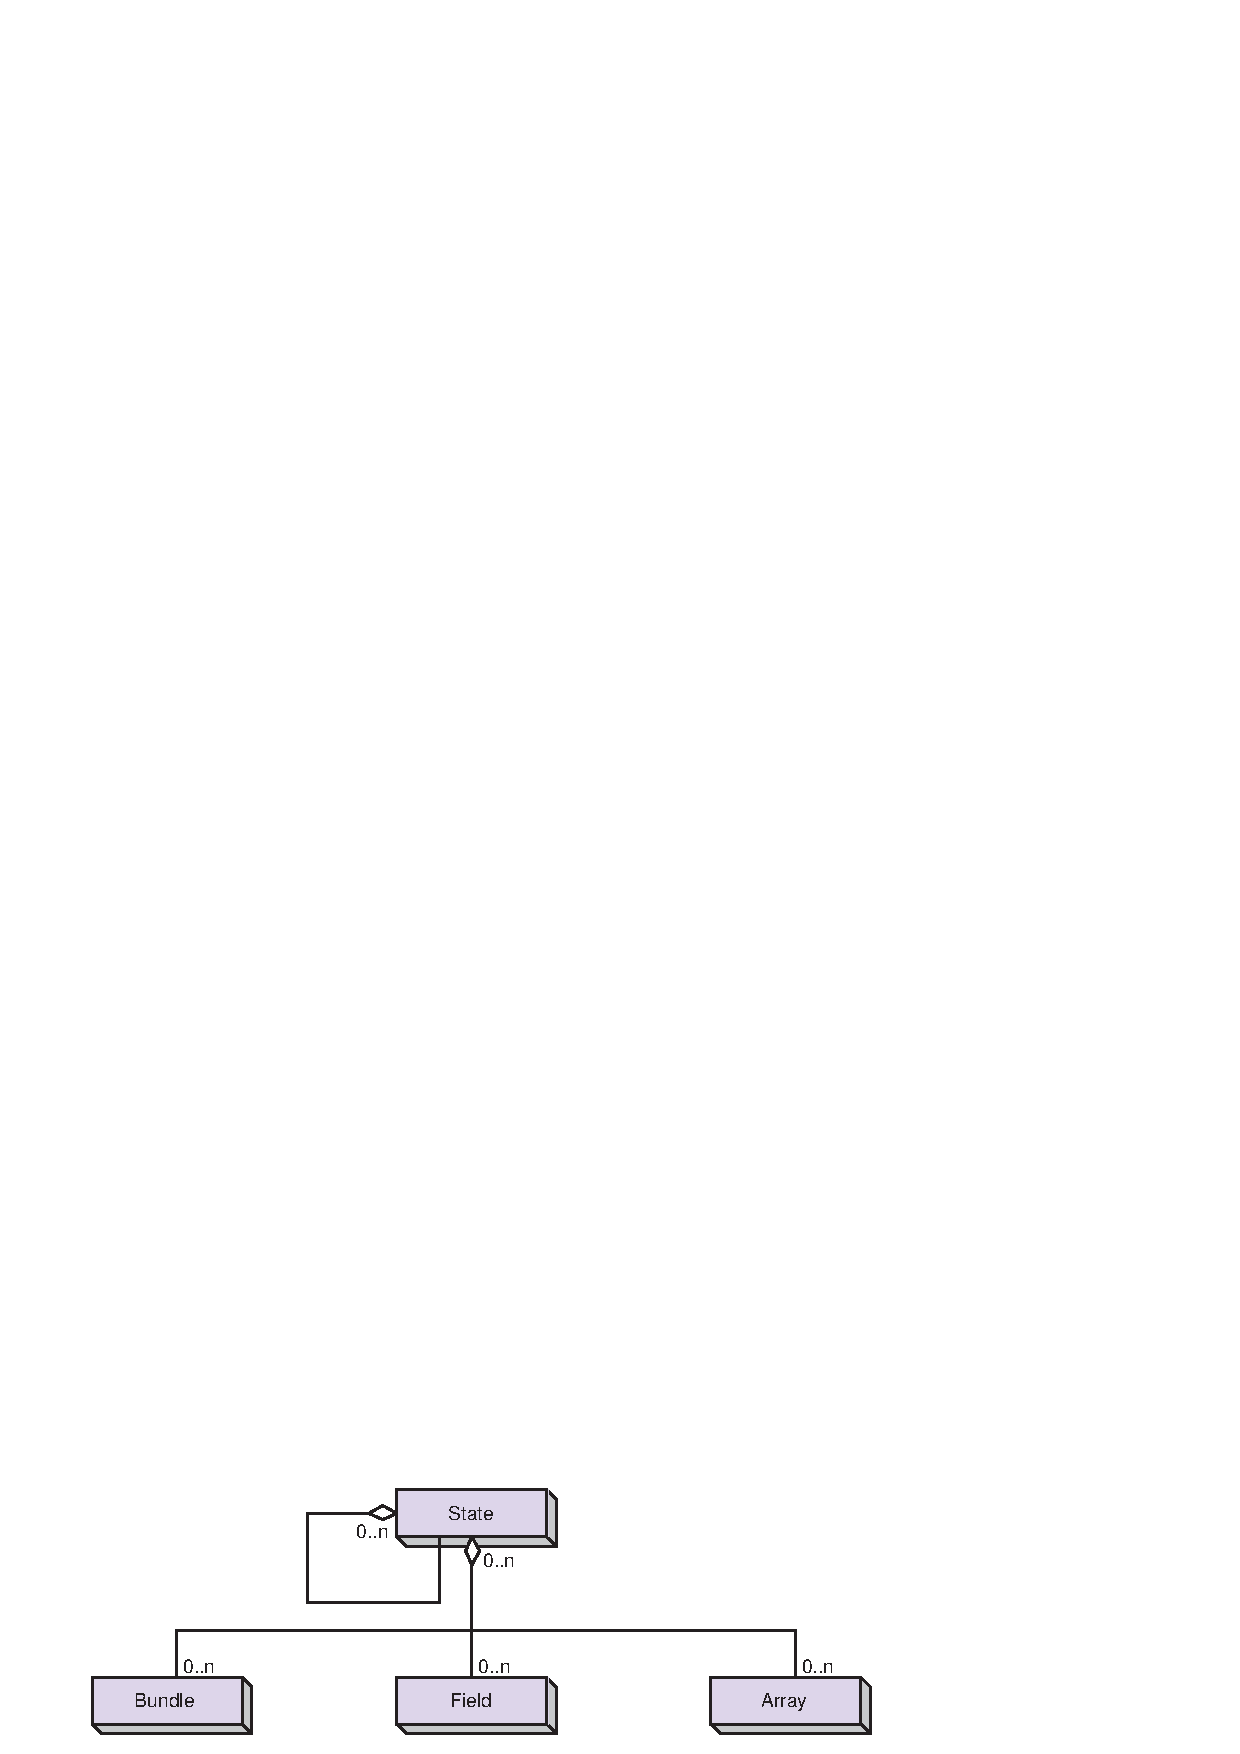
\includegraphics{State_obj}   
\end{center}

\subsection{Class API}
%                **** IMPORTANT NOTICE *****
% This LaTeX file has been automatically produced by ProTeX v. 1.1
% Any changes made to this file will likely be lost next time
% this file is regenerated from its source. Send questions 
% to Arlindo da Silva, dasilva@gsfc.nasa.gov
 
\setlength{\oldparskip}{\parskip}
\setlength{\parskip}{1.5ex}
\setlength{\oldparindent}{\parindent}
\setlength{\parindent}{0pt}
\setlength{\oldbaselineskip}{\baselineskip}
\setlength{\baselineskip}{11pt}
 
%--------------------- SHORT-HAND MACROS ----------------------
\def\bv{\begin{verbatim}}
\def\ev{\end{verbatim}}
\def\be{\begin{equation}}
\def\ee{\end{equation}}
\def\bea{\begin{eqnarray}}
\def\eea{\end{eqnarray}}
\def\bi{\begin{itemize}}
\def\ei{\end{itemize}}
\def\bn{\begin{enumerate}}
\def\en{\end{enumerate}}
\def\bd{\begin{description}}
\def\ed{\end{description}}
\def\({\left (}
\def\){\right )}
\def\[{\left [}
\def\]{\right ]}
\def\<{\left  \langle}
\def\>{\right \rangle}
\def\cI{{\cal I}}
\def\diag{\mathop{\rm diag}}
\def\tr{\mathop{\rm tr}}
%-------------------------------------------------------------

\markboth{Left}{Source File: ESMC\_State.h,  Date: Tue May  5 21:00:08 MDT 2020
}

 
%/////////////////////////////////////////////////////////////
\subsubsection [ESMC\_StateAddArray] {ESMC\_StateAddArray - Add an Array object to a State}


  
\bigskip{\sf INTERFACE:}
\begin{verbatim} int ESMC_StateAddArray(
   ESMC_State state,   // in
   ESMC_Array array    // in
 );\end{verbatim}{\em RETURN VALUE:}
\begin{verbatim}    Return code; equals ESMF_SUCCESS if there are no errors.\end{verbatim}
{\sf DESCRIPTION:\\ }


  
    Add an Array object to a {\tt ESMC\_State} object.
  
    The arguments are:
    \begin{description}
    \item[state]
      The State object.
    \item[array]
      The Array object to be included within the State.
    \end{description}
   
%/////////////////////////////////////////////////////////////
 
\mbox{}\hrulefill\ 
 
\subsubsection [ESMC\_StateAddField] {ESMC\_StateAddField - Add a Field object to a State}


  
\bigskip{\sf INTERFACE:}
\begin{verbatim} int ESMC_StateAddField(
   ESMC_State state,   // in
   ESMC_Field field    // in
 );\end{verbatim}{\em RETURN VALUE:}
\begin{verbatim}    Return code; equals ESMF_SUCCESS if there are no errors.\end{verbatim}
{\sf DESCRIPTION:\\ }


  
    Add an Array object to a {\tt ESMC\_State} object.
  
    The arguments are:
    \begin{description}
    \item[state]
      The State object.
    \item[array]
      The Array object to be included within the State.
    \end{description}
   
%/////////////////////////////////////////////////////////////
 
\mbox{}\hrulefill\ 
 
\subsubsection [ESMC\_StateCreate] {ESMC\_StateCreate - Create an Array}


  
\bigskip{\sf INTERFACE:}
\begin{verbatim} ESMC_State ESMC_StateCreate(
   const char *name,  // in
   int *rc            // out
 );\end{verbatim}{\em RETURN VALUE:}
\begin{verbatim}    Newly created ESMC_State object.\end{verbatim}
{\sf DESCRIPTION:\\ }


  
    Create an {\tt ESMC\_State} object.
  
    The arguments are:
    \begin{description}
    \item[{[name]}]
      The name for the State object. If not specified, i.e. NULL,
      a default unique name will be generated: "StateNNN" where NNN
      is a unique sequence number from 001 to 999.
    \item[rc]
      Return code; equals {\tt ESMF\_SUCCESS} if there are no errors.
    \end{description}
   
%/////////////////////////////////////////////////////////////
 
\mbox{}\hrulefill\ 
 
\subsubsection [ESMC\_StateDestroy] {ESMC\_StateDestroy - Destroy a State}


  
\bigskip{\sf INTERFACE:}
\begin{verbatim} int ESMC_StateDestroy(
   ESMC_State *state    // in
 );\end{verbatim}{\em RETURN VALUE:}
\begin{verbatim}    Return code; equals ESMF_SUCCESS if there are no errors.\end{verbatim}
{\sf DESCRIPTION:\\ }


  
    Destroy a {\tt ESMC\_State} object.
  
    The arguments are:
    \begin{description}
    \item[state]
      The State to be destroyed.
    \end{description}
   
%/////////////////////////////////////////////////////////////
 
\mbox{}\hrulefill\ 
 
\subsubsection [ESMC\_StateGetArray] {ESMC\_StateGetArray - Obtains an Array object from a State}


  
\bigskip{\sf INTERFACE:}
\begin{verbatim} int ESMC_StateGetArray(
   ESMC_State state,    // in
   const char *name,    // in
   ESMC_Array *array    // out
 );\end{verbatim}{\em RETURN VALUE:}
\begin{verbatim}    Return code; equals ESMF_SUCCESS if there are no errors.\end{verbatim}
{\sf DESCRIPTION:\\ }


  
    Obtain a pointer to an {\tt ESMC\_Array} object contained within
    a State.
  
    The arguments are:
    \begin{description}
    \item[state]
      The State object.
    \item[name]
      The name of the desired Array object.
    \item[array]
      A pointer to the Array object.
    \end{description}
   
%/////////////////////////////////////////////////////////////
 
\mbox{}\hrulefill\ 
 
\subsubsection [ESMC\_StateGetField] {ESMC\_StateGetField - Obtains a Field object from a State}


  
\bigskip{\sf INTERFACE:}
\begin{verbatim} int ESMC_StateGetField(
   ESMC_State state,    // in
   const char *name,    // in
   ESMC_Field *field    // out
 );\end{verbatim}{\em RETURN VALUE:}
\begin{verbatim}    Return code; equals ESMF_SUCCESS if there are no errors.\end{verbatim}
{\sf DESCRIPTION:\\ }


  
    Obtain a pointer to a {\tt ESMC\_Field} object contained within
    a State.
  
    The arguments are:
    \begin{description}
    \item[state]
      The State object.
    \item[name]
      The name of the desired Field object.
    \item[array]
      A pointer to the Field object.
    \end{description}
   
%/////////////////////////////////////////////////////////////
 
\mbox{}\hrulefill\ 
 
\subsubsection [ESMC\_StatePrint] {ESMC\_StatePrint - Print the contents of a State}


  
\bigskip{\sf INTERFACE:}
\begin{verbatim} int ESMC_StatePrint(
   ESMC_State state    // in
 );\end{verbatim}{\em RETURN VALUE:}
\begin{verbatim}    Return code; equals ESMF_SUCCESS if there are no errors.\end{verbatim}
{\sf DESCRIPTION:\\ }


  
    Prints the contents of a {\tt ESMC\_State} object.
  
    The arguments are:
    \begin{description}
    \item[state]
      The State to be printed.
    \end{description}
  
%...............................................................
\setlength{\parskip}{\oldparskip}
\setlength{\parindent}{\oldparindent}
\setlength{\baselineskip}{\oldbaselineskip}

%TODO:FIELDINTEGRATION Restore StateGet methods
%\subsection{Class API: State Overloads for Fortran Arrays}
%#ifdef STANDALONE
%%                **** IMPORTANT NOTICE *****
% This LaTeX file has been automatically produced by ProTeX v. 1.1
% Any changes made to this file will likely be lost next time
% this file is regenerated from its source. Send questions 
% to Arlindo da Silva, dasilva@gsfc.nasa.gov
 
\setlength{\oldparskip}{\parskip}
\setlength{\parskip}{1.5ex}
\setlength{\oldparindent}{\parindent}
\setlength{\parindent}{0pt}
\setlength{\oldbaselineskip}{\baselineskip}
\setlength{\baselineskip}{11pt}
 
%--------------------- SHORT-HAND MACROS ----------------------
\def\bv{\begin{verbatim}}
\def\ev{\end{verbatim}}
\def\be{\begin{equation}}
\def\ee{\end{equation}}
\def\bea{\begin{eqnarray}}
\def\eea{\end{eqnarray}}
\def\bi{\begin{itemize}}
\def\ei{\end{itemize}}
\def\bn{\begin{enumerate}}
\def\en{\end{enumerate}}
\def\bd{\begin{description}}
\def\ed{\end{description}}
\def\({\left (}
\def\){\right )}
\def\[{\left [}
\def\]{\right ]}
\def\<{\left  \langle}
\def\>{\right \rangle}
\def\cI{{\cal I}}
\def\diag{\mathop{\rm diag}}
\def\tr{\mathop{\rm tr}}
%-------------------------------------------------------------

\markboth{Left}{Source File: ESMF\_StateGet.F90,  Date: Tue May  5 21:00:08 MDT 2020
}

 
%/////////////////////////////////////////////////////////////
\subsubsection [ESMF\_StateGetDataPointer] {ESMF\_StateGetDataPointer - Retrieve Fortran pointer directly from a State }


   
\bigskip{\sf INTERFACE:}
\begin{verbatim}   ! Private name; call using ESMF_StateGetDataPointer() 
   subroutine ESMF_StateGetDataPointer<rank><type><kind>(state, itemName, 
   dataPointer, datacopyflag, nestedStateName, rc) 
   \end{verbatim}{\em ARGUMENTS:}
\begin{verbatim}   type(ESMF_State), intent(in) :: state 
   character(len=*), intent(in) :: itemName 
   <type> (ESMF_KIND_<kind>), dimension(<rank>), pointer :: dataPointer 
   type(ESMF_DataCopy_Flag), intent(in), optional :: datacopyflag 
   character(len=*), intent(in), optional :: nestedStateName 
   integer, intent(out), optional :: rc 
   
   \end{verbatim}
{\sf STATUS:}
   \begin{itemize} 
   \item\apiStatusCompatibleVersion{5.2.0r} 
   \end{itemize} 
   
{\sf DESCRIPTION:\\ }

 
   Retrieves data from a state, returning a direct Fortran pointer to 
   the data array. 
   Valid type/kind/rank combinations supported by the 
   framework are: ranks 1 to 7, type real of kind *4 or *8, 
   and type integer of kind *1, *2, *4, or *8. 
   
   The arguments are: 
   \begin{description} 
   \item[state] 
   The {\tt ESMF\_State} to query. 
   \item[itemName] 
   The name of the FieldBundle, Field, or Array to return data from. 
   \item[dataPointer] 
   An unassociated Fortran pointer of the proper Type, Kind, and Rank as the data 
   in the State. When this call returns successfully, the pointer will now reference 
   the data in the State. This is either a reference or a copy, depending on the 
   setting of the following argument. The default is to return a reference. 
   \item[{[datacopyflag]}] 
   Defaults to {\tt ESMF\_DATACOPY\_REFERENCE}. If set to {\tt ESMF\_DATACOPY\_VALUE}, a separate 
   copy of the data will be made and the pointer will point at the copy. 
   \item[{[nestedStateName]}] 
   Optional. If multiple states are present, a specific state name must be given. 
   \item[{[fieldName]}] 
   Optional. If {\tt itemName} refers to a fieldbundle then the name of the field 
   in the fieldbundle must also be given. 
   \item[{[rc]}] 
   Return code; equals {\tt ESMF\_SUCCESS} if there are no errors. 
   \end{description} 
   
%...............................................................
\setlength{\parskip}{\oldparskip}
\setlength{\parindent}{\oldparindent}
\setlength{\baselineskip}{\oldbaselineskip}

%%                **** IMPORTANT NOTICE *****
% This LaTeX file has been automatically produced by ProTeX v. 1.1
% Any changes made to this file will likely be lost next time
% this file is regenerated from its source. Send questions 
% to Arlindo da Silva, dasilva@gsfc.nasa.gov
 
\setlength{\oldparskip}{\parskip}
\setlength{\parskip}{1.5ex}
\setlength{\oldparindent}{\parindent}
\setlength{\parindent}{0pt}
\setlength{\oldbaselineskip}{\baselineskip}
\setlength{\baselineskip}{11pt}
 
%--------------------- SHORT-HAND MACROS ----------------------
\def\bv{\begin{verbatim}}
\def\ev{\end{verbatim}}
\def\be{\begin{equation}}
\def\ee{\end{equation}}
\def\bea{\begin{eqnarray}}
\def\eea{\end{eqnarray}}
\def\bi{\begin{itemize}}
\def\ei{\end{itemize}}
\def\bn{\begin{enumerate}}
\def\en{\end{enumerate}}
\def\bd{\begin{description}}
\def\ed{\end{description}}
\def\({\left (}
\def\){\right )}
\def\[{\left [}
\def\]{\right ]}
\def\<{\left  \langle}
\def\>{\right \rangle}
\def\cI{{\cal I}}
\def\diag{\mathop{\rm diag}}
\def\tr{\mathop{\rm tr}}
%-------------------------------------------------------------

\markboth{Left}{Source File: ESMF\_StateGet.F90,  Date: Tue May  5 21:00:08 MDT 2020
}

 
%/////////////////////////////////////////////////////////////
\subsubsection [ESMF\_StateGetDataPointer] {ESMF\_StateGetDataPointer - Retrieve Fortran pointer directly from a State }


   
\bigskip{\sf INTERFACE:}
\begin{verbatim}   ! Private name; call using ESMF_StateGetDataPointer() 
   subroutine ESMF_StateGetDataPointer<rank><type><kind>(state, itemName, 
   dataPointer, datacopyflag, nestedStateName, rc) 
   \end{verbatim}{\em ARGUMENTS:}
\begin{verbatim}   type(ESMF_State), intent(in) :: state 
   character(len=*), intent(in) :: itemName 
   <type> (ESMF_KIND_<kind>), dimension(<rank>), pointer :: dataPointer 
   type(ESMF_DataCopy_Flag), intent(in), optional :: datacopyflag 
   character(len=*), intent(in), optional :: nestedStateName 
   integer, intent(out), optional :: rc 
   
   \end{verbatim}
{\sf STATUS:}
   \begin{itemize} 
   \item\apiStatusCompatibleVersion{5.2.0r} 
   \end{itemize} 
   
{\sf DESCRIPTION:\\ }

 
   Retrieves data from a state, returning a direct Fortran pointer to 
   the data array. 
   Valid type/kind/rank combinations supported by the 
   framework are: ranks 1 to 7, type real of kind *4 or *8, 
   and type integer of kind *1, *2, *4, or *8. 
   
   The arguments are: 
   \begin{description} 
   \item[state] 
   The {\tt ESMF\_State} to query. 
   \item[itemName] 
   The name of the FieldBundle, Field, or Array to return data from. 
   \item[dataPointer] 
   An unassociated Fortran pointer of the proper Type, Kind, and Rank as the data 
   in the State. When this call returns successfully, the pointer will now reference 
   the data in the State. This is either a reference or a copy, depending on the 
   setting of the following argument. The default is to return a reference. 
   \item[{[datacopyflag]}] 
   Defaults to {\tt ESMF\_DATACOPY\_REFERENCE}. If set to {\tt ESMF\_DATACOPY\_VALUE}, a separate 
   copy of the data will be made and the pointer will point at the copy. 
   \item[{[nestedStateName]}] 
   Optional. If multiple states are present, a specific state name must be given. 
   \item[{[fieldName]}] 
   Optional. If {\tt itemName} refers to a fieldbundle then the name of the field 
   in the fieldbundle must also be given. 
   \item[{[rc]}] 
   Return code; equals {\tt ESMF\_SUCCESS} if there are no errors. 
   \end{description} 
   
%...............................................................
\setlength{\parskip}{\oldparskip}
\setlength{\parindent}{\oldparindent}
\setlength{\baselineskip}{\oldbaselineskip}

%#elif defined(1)
%%                **** IMPORTANT NOTICE *****
% This LaTeX file has been automatically produced by ProTeX v. 1.1
% Any changes made to this file will likely be lost next time
% this file is regenerated from its source. Send questions 
% to Arlindo da Silva, dasilva@gsfc.nasa.gov
 
\setlength{\oldparskip}{\parskip}
\setlength{\parskip}{1.5ex}
\setlength{\oldparindent}{\parindent}
\setlength{\parindent}{0pt}
\setlength{\oldbaselineskip}{\baselineskip}
\setlength{\baselineskip}{11pt}
 
%--------------------- SHORT-HAND MACROS ----------------------
\def\bv{\begin{verbatim}}
\def\ev{\end{verbatim}}
\def\be{\begin{equation}}
\def\ee{\end{equation}}
\def\bea{\begin{eqnarray}}
\def\eea{\end{eqnarray}}
\def\bi{\begin{itemize}}
\def\ei{\end{itemize}}
\def\bn{\begin{enumerate}}
\def\en{\end{enumerate}}
\def\bd{\begin{description}}
\def\ed{\end{description}}
\def\({\left (}
\def\){\right )}
\def\[{\left [}
\def\]{\right ]}
\def\<{\left  \langle}
\def\>{\right \rangle}
\def\cI{{\cal I}}
\def\diag{\mathop{\rm diag}}
\def\tr{\mathop{\rm tr}}
%-------------------------------------------------------------

\markboth{Left}{Source File: ESMF\_StateGet.F90,  Date: Tue May  5 21:00:08 MDT 2020
}

 
%/////////////////////////////////////////////////////////////
\subsubsection [ESMF\_StateGetDataPointer] {ESMF\_StateGetDataPointer - Retrieve Fortran pointer directly from a State }


   
\bigskip{\sf INTERFACE:}
\begin{verbatim}   ! Private name; call using ESMF_StateGetDataPointer() 
   subroutine ESMF_StateGetDataPointer<rank><type><kind>(state, itemName, 
   dataPointer, datacopyflag, nestedStateName, rc) 
   \end{verbatim}{\em ARGUMENTS:}
\begin{verbatim}   type(ESMF_State), intent(in) :: state 
   character(len=*), intent(in) :: itemName 
   <type> (ESMF_KIND_<kind>), dimension(<rank>), pointer :: dataPointer 
   type(ESMF_DataCopy_Flag), intent(in), optional :: datacopyflag 
   character(len=*), intent(in), optional :: nestedStateName 
   integer, intent(out), optional :: rc 
   
   \end{verbatim}
{\sf STATUS:}
   \begin{itemize} 
   \item\apiStatusCompatibleVersion{5.2.0r} 
   \end{itemize} 
   
{\sf DESCRIPTION:\\ }

 
   Retrieves data from a state, returning a direct Fortran pointer to 
   the data array. 
   Valid type/kind/rank combinations supported by the 
   framework are: ranks 1 to 7, type real of kind *4 or *8, 
   and type integer of kind *1, *2, *4, or *8. 
   
   The arguments are: 
   \begin{description} 
   \item[state] 
   The {\tt ESMF\_State} to query. 
   \item[itemName] 
   The name of the FieldBundle, Field, or Array to return data from. 
   \item[dataPointer] 
   An unassociated Fortran pointer of the proper Type, Kind, and Rank as the data 
   in the State. When this call returns successfully, the pointer will now reference 
   the data in the State. This is either a reference or a copy, depending on the 
   setting of the following argument. The default is to return a reference. 
   \item[{[datacopyflag]}] 
   Defaults to {\tt ESMF\_DATACOPY\_REFERENCE}. If set to {\tt ESMF\_DATACOPY\_VALUE}, a separate 
   copy of the data will be made and the pointer will point at the copy. 
   \item[{[nestedStateName]}] 
   Optional. If multiple states are present, a specific state name must be given. 
   \item[{[fieldName]}] 
   Optional. If {\tt itemName} refers to a fieldbundle then the name of the field 
   in the fieldbundle must also be given. 
   \item[{[rc]}] 
   Return code; equals {\tt ESMF\_SUCCESS} if there are no errors. 
   \end{description} 
   
%...............................................................
\setlength{\parskip}{\oldparskip}
\setlength{\parindent}{\oldparindent}
\setlength{\baselineskip}{\oldbaselineskip}

%#endif
%#include "../Superstructure/AttachMethods/doc/AttachMethods_crefdoc.ctex"
%#include "../Superstructure/WebServices/doc/WebServices_crefdoc.ctex"
%+==============================================================================
\newpage
\begin{htmlonly}
\addcontentsline{toc}{part}{Infrastructure: Fields and Grids}
\end{htmlonly}
\part{Infrastructure: Fields and Grids}
\newpage
%\section{Overview of Infrastructure Data Classes}
% $Id$

%TODO: This file started as an exact copy of the Fortran version of this file.
%TODO: Changes were made to correctly reflect the current status of the C API.
%TODO: Eventually this file should be removed again and replaced by a single
%TODO: generic version that can be included for both Fortran and C refdocs.

\section{Overview of Infrastructure Data Handling}

The ESMF infrastructure data classes are part of the framework's 
hierarchy of structures for handling Earth system model data and 
metadata on parallel platforms.  The hierarchy is in complexity; the 
simplest data class in the infrastructure represents a distributed data
array and the most complex data class represents a bundle of physical 
fields that are discretized on the same grid.  However, the current C API 
does not support bundled data structures yet. Array and Field are the two
data classes offered by the ESMF C language binding.  Data class methods 
are called both from user-written code and from other classes 
internal to the framework. 

Data classes are distributed over {\bf DE}s, or {\bf Decomposition Elements}.  
A DE represents a piece of a decomposition.  A DELayout is a collection
of DEs with some associated connectivity that describes a specific 
distribution.  For example, the distribution of a grid divided 
into four segments in the x-dimension would be expressed in ESMF as
a DELayout with four DEs lying along an x-axis. This abstract concept 
enables a data decomposition to be defined in 
terms of threads, MPI processes, virtual decomposition elements, or
combinations of these without changes to user code.  This is a
primary strategy for ensuring optimal performance and portability
for codes using the ESMF for communications.

ESMF data classes provide a standard,
convenient way for developers to collect together information 
related to model or observational data.  The information assembled 
in a data class includes a data pointer, a set of attributes 
(e.g. units, although attributes can also be user-defined), and a 
description of an associated grid.  The same set of information within 
an ESMF data object can be used by the framework to arrange 
intercomponent data transfers, to perform I/O, for communications
such as gathers and scatters, for simplification of interfaces 
within user code, for debugging, and for other functions.  
This unifies and organizes codes overall so that the user need not
define different representations of metadata for the same field 
for I/O and for component coupling.  

Since it is critical that users be able to introduce ESMF into their
codes easily and incrementally, ESMF data classes can be created based 
on native Fortran pointers.  Likewise, there are methods for retrieving 
native Fortran pointers from within ESMF data objects.  This allows
the user to perform allocations using ESMF, and to retrieve Fortran
arrays later for optimized model calculations.  The ESMF data classes 
do not have associated differential operators or other mathematical 
methods.

For flexibility, it is not necessary to build an ESMF data object 
all at once.  For example, it's possible to create a 
field but to defer allocation of the associated field data until 
a later time.


\begin{center}  
\begin{tabular}{|p{6in}|}
\hline
\vspace{.01in}
{\bf Key Features} \\[.01in]
Hierarchy of data structures designed specifically for the Earth 
system domain and high performance, parallel computing. \\
Multi-use ESMF structures simplify user code overall. \\
Data objects support incremental construction and deferred allocation. \\ 
Native Fortran arrays can be associated with or retrieved from ESMF data
objects, for ease of adoption, convenience, and performance. \\[.03in] \hline
\end{tabular}
\end{center}

\subsection{Infrastructure Data Classes}

The main classes that are used for model and observational data manipulation
are as follows:

\begin{itemize}

\item {\bf Array}  An ESMF Array contains a data pointer, 
information about its associated datatype, precision, and 
dimension.  

Data elements in Arrays are partitioned into categories 
defined by the role the data element plays in distributed halo 
operations.  Haloing - sometimes called ghosting - is the 
practice of copying portions of array data to multiple memory 
locations to ensure that data dependencies can be satisfied 
quickly when performing a calculation.  ESMF Arrays contain 
an {\bf exclusive} domain, which contains data elements
updated exclusively and definitively by a given DE; a 
{\bf computational} domain, which contains all data elements
with values that are updated by the DE in computations; and 
a {\bf total} domain, which includes both the computational 
domain and data elements from other DEs which may be read 
but are not updated in computations.

\item {\bf Field}  A Field holds model and/or observational 
data together with its underlying grid or set of spatial 
locations.  It provides methods for configuration, 
initialization, setting and retrieving data values, 
data I/O, data regridding, and manipulation of attributes.

\end{itemize}










%\section{Design and Implementation Notes}
% $Id$

%TODO: This file started as an exact copy of the Fortran version of this file.
%TODO: Changes were made to correctly reflect the current status of the C API.
%TODO: Eventually this file should be removed again and replaced by a single
%TODO: generic version that can be included for both Fortran and C refdocs.

\subsection{Design and Implementation Notes}

\begin{enumerate}

\item In communication methods such as Regrid, Redist, Scatter, etc. 
the Field code cascades down through the Array code, so 
that the actual implementation exist in only one place in the source.

\end{enumerate}

\newpage
%#include "../Infrastructure/FieldBundle/doc/FieldBundle_crefdoc.ctex"
% $Id$
\bodytext{BGCOLOR=white LINK=#083194 VLINK=#21004A}
\section{Field Class}
\subsection{Description}
% $Id$

%TODO: This file started as an exact copy of the Fortran version of this file.
%TODO: Changes were made to correctly reflect the current status of the C API.
%TODO: Eventually this file should be removed again and replaced by a single
%TODO: generic version that can be included for both Fortran and C refdocs.

An ESMF Field represents a physical field, such as temperature.
The motivation for including Fields in ESMF is that bundles of 
Fields are the entities that are normally exchanged when coupling
Components.  

The ESMF Field class contains distributed and discretized field data, a reference 
to its associated grid, and metadata.  The Field class stores the grid {\it staggering}
for that physical field.
This is the relationship of how the data array of a field maps onto a grid 
(e.g. one item per
cell located at the cell center, one item per cell located at the NW
corner,  one item per cell vertex, etc.).  This means that different Fields
which are on the same underlying ESMF Grid but have different
staggerings can share the same Grid object without needing to replicate
it multiple times. 

Fields can be added to States for use in inter-Component
data communications.

Field communication capabilities include: data redistribution, regridding, scatter,
gather, sparse-matrix multiplication, and halo update.  These are discussed
in more detail in the documentation for the specific method calls.  
ESMF does not currently support vector fields, so the components of 
a vector field must be stored as separate Field objects.  

\subsection{Constants}
% $Id$

\subsubsection{ESMC\_REGRIDMETHOD}
\label{opt:cregridmethod}

{\sf DESCRIPTION:\\}  
Specify which interpolation method to use during regridding. 

The type of this flag is:

{\tt type(ESMC\_RegridMethod\_Flag)}

The valid values are:
\begin{description}
\item [ESMC\_REGRIDMETHOD\_BILINEAR]
      Bilinear interpolation. Destination value is a linear combination of the source values in the cell which contains the destination point. The weights for the linear combination are based on the distance of destination point from each source value. 
\item [ESMC\_REGRIDMETHOD\_PATCH]
      Higher-order patch recovery interpolation. Destination value is a weighted average of 2D polynomial patches constructed from cells surrounding the source cell which contains the destination point. This method typically results in better approximations to values and derivatives than bilinear. However, because of its larger stencil, it also results in a much larger interpolation matrix (and thus routeHandle) than the bilinear. 
\item [ESMC\_REGRIDMETHOD\_NEAREST\_STOD]
      In this version of nearest neighbor interpolation each destination point is mapped to the closest source point. A given source point may go to multiple destination points, but no destination point will receive input from more than one source point. 
\item [ESMC\_REGRIDMETHOD\_NEAREST\_DTOS]
      In this version of nearest neighbor interpolation each source point is mapped to the closest destination point. A given destination point may receive input from multiple source points, but no source point will go to more than one destination point. 
\item [ESMC\_REGRIDMETHOD\_CONSERVE]
      First-order conservative interpolation. The main purpose of this method is to preserve the integral of the field between the source and destination. 
      Will typically give a less accurate approximation to the individual field values than the bilinear or patch methods. The value of a destination cell is calculated as the weighted sum of the values of the source cells that it overlaps. The weights are determined by the amount the source cell overlaps the destination cell. Needs corner coordinate values to be provided in the Grid. Currently only works for Fields created on the Grid center stagger or the Mesh element location. 
\item [ESMC\_REGRIDMETHOD\_CONSERVE\_2ND]
      Second-order conservative interpolation. As with first-order, preserves the integral of the value between the source and destination. However, typically produces a smoother more accurate result than first-order. Also like first-order, the value of a destination cell is calculated as the weighted sum of the values of the source cells that it overlaps. However, second-order also includes additional terms to take into account the gradient of the field across the source cell. Needs corner coordinate values to be provided in the Grid. Currently only works for Fields created on the Grid center stagger or the Mesh element location. 
\end{description}

\subsection{Use and Examples}
% $Id$

%TODO: This file started as an exact copy of the Fortran version of this file.
%TODO: Changes were made to correctly reflect the current status of the C API.
%TODO: Eventually this file should be removed again and replaced by a single
%TODO: generic version that can be included for both Fortran and C refdocs.

%\subsection{Use and Examples}

A Field serves as an annotator of data, since it carries 
a description of the grid it is associated with and metadata 
such as name and units.  Fields can be used in this capacity
alone, as convenient, descriptive containers into which arrays 
can be placed and retrieved.  However, for most codes the primary 
use of Fields is in the context of import and export States,
which are the objects that carry coupling information between 
Components.  Fields enable data to be self-describing, and a
State holding ESMF Fields contains data in a standard format
that can be queried and manipulated.  

The sections below go into more detail about Field usage.

\subsubsection{Field create and destroy}

Fields can be created and destroyed at any time during 
application execution.  However, these Field methods require 
some time to complete.  We do not recommend that the user
create or destroy Fields inside performance-critical 
computational loops.

All versions of the {\tt ESMC\_FieldCreate()} 
routines require a Mesh object as input.
The Mesh contains the information needed to know which 
Decomposition Elements (DEs) are participating in 
the processing of this Field, and which subsets of the data
are local to a particular DE.

The details of how the create process happens depend
on which of the variants of the {\tt ESMC\_FieldCreate()} 
call is used.

When finished with an {\tt ESMC\_Field}, the {\tt ESMC\_FieldDestroy} method
removes it.  However, the objects inside the {\tt ESMC\_Field}
created externally should be destroyed separately, 
since objects can be added to
more than one {\tt ESMC\_Field}.  For example, the same {\tt ESMF\_Mesh}
can be referenced by multiple {\tt ESMC\_Field}s.  In this case the
internal Mesh is not deleted by the {\tt ESMC\_FieldDestroy} call.

%%                **** IMPORTANT NOTICE *****
% This LaTeX file has been automatically produced by ProTeX v. 1.1
% Any changes made to this file will likely be lost next time
% this file is regenerated from its source. Send questions 
% to Arlindo da Silva, dasilva@gsfc.nasa.gov
 
\setlength{\oldparskip}{\parskip}
\setlength{\parskip}{1.5ex}
\setlength{\oldparindent}{\parindent}
\setlength{\parindent}{0pt}
\setlength{\oldbaselineskip}{\baselineskip}
\setlength{\baselineskip}{11pt}
 
%--------------------- SHORT-HAND MACROS ----------------------
\def\bv{\begin{verbatim}}
\def\ev{\end{verbatim}}
\def\be{\begin{equation}}
\def\ee{\end{equation}}
\def\bea{\begin{eqnarray}}
\def\eea{\end{eqnarray}}
\def\bi{\begin{itemize}}
\def\ei{\end{itemize}}
\def\bn{\begin{enumerate}}
\def\en{\end{enumerate}}
\def\bd{\begin{description}}
\def\ed{\end{description}}
\def\({\left (}
\def\){\right )}
\def\[{\left [}
\def\]{\right ]}
\def\<{\left  \langle}
\def\>{\right \rangle}
\def\cI{{\cal I}}
\def\diag{\mathop{\rm diag}}
\def\tr{\mathop{\rm tr}}
%-------------------------------------------------------------

\markboth{Left}{Source File: ESMF\_FieldEx.F90,  Date: Tue May  5 21:00:02 MDT 2020
}

 
%/////////////////////////////////////////////////////////////

  \subsubsection{Get Fortran data pointer, bounds, and counts information from a Field}
  \label{sec:field:usage:field_get_dataptr}
  
    A user can get bounds and counts information from an {\tt ESMF\_Field}
    through the {\tt ESMF\_FieldGet()} interface.  Also available through this interface
    is the intrinsic
    Fortran data pointer contained in the internal {\tt ESMF\_Array} object
    of an {\tt ESMF\_Field}. The bounds and counts information are DE specific
    for the associated Fortran data pointer.
  
    For a better discussion of the terminologies, bounds and widths in ESMF
    e.g. exclusive, computational, total bounds
    for the lower and upper corner of data region, etc.., user can refer to
    the explanation of these concepts for Grid and Array in their respective sections
    in the {\it Reference Manual}, e.g. Section \ref{Array_regions_and_default_bounds} on Array
    and Section \ref{sec:grid:usage:bounds} on Grid.
  
    In this example, we first create a 3D Field based on a 3D Grid and Array.
    Then we use the {\tt ESMF\_FieldGet()} interface to retrieve the data pointer,
    potentially updating or verifying its values. We also retrieve the bounds and counts
    information of the 3D Field to assist in data element iteration.
   
%/////////////////////////////////////////////////////////////

 \begin{verbatim}
    xdim = 180
    ydim = 90
    zdim = 50

    ! create a 3D data Field from a Grid and Array.
    ! first create a Grid
    grid3d = ESMF_GridCreateNoPeriDim(minIndex=(/1,1,1/), &
            maxIndex=(/xdim,ydim,zdim/), &
            regDecomp=(/2,2,1/), name="grid", rc=rc)
    if (rc /= ESMF_SUCCESS) call ESMF_Finalize(endflag=ESMF_END_ABORT)

    call ESMF_GridGet(grid=grid3d, staggerloc=ESMF_STAGGERLOC_CENTER, &
           distgrid=distgrid3d, rc=rc)
    if (rc /= ESMF_SUCCESS) call ESMF_Finalize(endflag=ESMF_END_ABORT)

    call ESMF_GridGetFieldBounds(grid=grid3d, localDe=0, &
        staggerloc=ESMF_STAGGERLOC_CENTER, totalCount=fa_shape, rc=rc)
    if (rc /= ESMF_SUCCESS) call ESMF_Finalize(endflag=ESMF_END_ABORT)

    allocate(farray(fa_shape(1), fa_shape(2), fa_shape(3)) )

    ! create an Array
    array3d = ESMF_ArrayCreate(distgrid3d, farray, &
        indexflag=ESMF_INDEX_DELOCAL, rc=rc)
    if (rc /= ESMF_SUCCESS) call ESMF_Finalize(endflag=ESMF_END_ABORT)

    ! create a Field
    field = ESMF_FieldCreate(grid=grid3d, array=array3d, rc=rc)
    if (rc /= ESMF_SUCCESS) call ESMF_Finalize(endflag=ESMF_END_ABORT)

    ! retrieve the Fortran data pointer from the Field
    call ESMF_FieldGet(field=field, localDe=0, farrayPtr=farray1, rc=rc)
    if (rc /= ESMF_SUCCESS) call ESMF_Finalize(endflag=ESMF_END_ABORT)

    ! retrieve the Fortran data pointer from the Field and bounds
    call ESMF_FieldGet(field=field, localDe=0, farrayPtr=farray1, &
        computationalLBound=compLBnd, computationalUBound=compUBnd, &
        exclusiveLBound=exclLBnd, exclusiveUBound=exclUBnd, &
        totalLBound=totalLBnd, totalUBound=totalUBnd, &
        computationalCount=comp_count, &
        exclusiveCount=excl_count, &
        totalCount=total_count, &
        rc=rc)


    ! iterate through the total bounds of the field data pointer
    do k = totalLBnd(3), totalUBnd(3)
        do j = totalLBnd(2), totalUBnd(2)
            do i = totalLBnd(1), totalUBnd(1)
                farray1(i, j, k) = sin(2*i/total_count(1)*PI) + &
                    sin(4*j/total_count(2)*PI) + &
                    sin(8*k/total_count(2)*PI)
            enddo
        enddo
    enddo
 
\end{verbatim}
 
%/////////////////////////////////////////////////////////////

  \subsubsection{Get Grid, Array, and other information from a Field}
  \label{sec:field:usage:field_get_default}
  
    A user can get the internal {\tt ESMF\_Grid} and {\tt ESMF\_Array}
    from a {\tt ESMF\_Field}.  Note that the user should not issue any destroy command
    on the retrieved grid or array object since they are referenced
    from within the {\tt ESMF\_Field}. The retrieved objects should be used
    in a read-only fashion to query additional information not directly
    available through the {\tt ESMF\_FieldGet()} interface.
   
%/////////////////////////////////////////////////////////////

 \begin{verbatim}
    call ESMF_FieldGet(field, grid=grid, array=array, &
        typekind=typekind, dimCount=dimCount, staggerloc=staggerloc, &
        gridToFieldMap=gridToFieldMap, &
        ungriddedLBound=ungriddedLBound, ungriddedUBound=ungriddedUBound, &
        totalLWidth=totalLWidth, totalUWidth=totalUWidth, &
        name=name, &
        rc=rc)
 
\end{verbatim}
 
%/////////////////////////////////////////////////////////////

  \subsubsection{Create a Field with a Grid, typekind, and rank}
  \label{sec:field:usage:create_grid_tkr}
  
    A user can create an {\tt ESMF\_Field} from an {\tt ESMF\_Grid} and
    typekind/rank.
    This create method associates the two objects.
  
    We first create a Grid with a regular distribution that is
    10x20 index in 2x2 DEs.  This version of Field create simply
    associates the data with the Grid.  The data is referenced
    explicitly on a regular 2x2 uniform grid.
    Finally we create a Field from
    the Grid, typekind, rank, and a user specified StaggerLoc.
  
    This example also illustrates a typical use of this Field creation
    method. By creating a Field from a Grid and typekind/rank, the
    user allows the ESMF library to create a internal Array in the Field.
    Then the user can use {\tt ESMF\_FieldGet()} to retrieve the Fortran
    data array
    and necessary bounds information to assign initial values to it. 
%/////////////////////////////////////////////////////////////

 \begin{verbatim}
    ! create a grid
    grid = ESMF_GridCreateNoPeriDim(minIndex=(/1,1/), maxIndex=(/10,20/), &
          regDecomp=(/2,2/), name="atmgrid", rc=rc)
    if (rc /= ESMF_SUCCESS) call ESMF_Finalize(endflag=ESMF_END_ABORT)

    ! create a Field from the Grid and arrayspec
    field1 = ESMF_FieldCreate(grid, typekind=ESMF_TYPEKIND_R4, &
        indexflag=ESMF_INDEX_DELOCAL, &
        staggerloc=ESMF_STAGGERLOC_CENTER, name="pressure", rc=rc)
    if (rc /= ESMF_SUCCESS) call ESMF_Finalize(endflag=ESMF_END_ABORT)

    call ESMF_FieldGet(field1, localDe=0, farrayPtr=farray2dd, &
        totalLBound=ftlb, totalUBound=ftub, totalCount=ftc, rc=rc)

    do i = ftlb(1), ftub(1)
        do j = ftlb(2), ftub(2)
            farray2dd(i, j) = sin(i/ftc(1)*PI) * cos(j/ftc(2)*PI)
        enddo
    enddo

    if (rc /= ESMF_SUCCESS) call ESMF_Finalize(endflag=ESMF_END_ABORT)
 
\end{verbatim}
 
%/////////////////////////////////////////////////////////////

  \subsubsection{Create a Field with a Grid and Arrayspec}
  \label{sec:field:usage:create_grid_arrayspec}
  
    A user can create an {\tt ESMF\_Field} from an {\tt ESMF\_Grid} and a
    {\tt ESMF\_Arrayspec} with corresponding rank and type.
    This create method associates the two objects.
  
    We first create a Grid with a regular distribution that is
    10x20 index in 2x2 DEs.  This version of Field create simply
    associates the data with the Grid.  The data is referenced
    explicitly on a regular 2x2 uniform grid.
    Then we create an ArraySpec.  Finally we create a Field from
    the Grid, ArraySpec, and a user specified StaggerLoc.
  
    This example also illustrates a typical use of this Field creation
    method. By creating a Field from a Grid and an ArraySpec, the
    user allows the ESMF library to create a internal Array in the Field.
    Then the user can use {\tt ESMF\_FieldGet()} to retrieve the Fortran
    data array
    and necessary bounds information to assign initial values to it. 
%/////////////////////////////////////////////////////////////

 \begin{verbatim}
    ! create a grid
    grid = ESMF_GridCreateNoPeriDim(minIndex=(/1,1/), maxIndex=(/10,20/), &
          regDecomp=(/2,2/), name="atmgrid", rc=rc)
    if (rc /= ESMF_SUCCESS) call ESMF_Finalize(endflag=ESMF_END_ABORT)

    ! setup arrayspec
    call ESMF_ArraySpecSet(arrayspec, 2, ESMF_TYPEKIND_R4, rc=rc)
    if (rc /= ESMF_SUCCESS) call ESMF_Finalize(endflag=ESMF_END_ABORT)

    ! create a Field from the Grid and arrayspec
    field1 = ESMF_FieldCreate(grid, arrayspec, &
         indexflag=ESMF_INDEX_DELOCAL, &
         staggerloc=ESMF_STAGGERLOC_CENTER, name="pressure", rc=rc)
    if (rc /= ESMF_SUCCESS) call ESMF_Finalize(endflag=ESMF_END_ABORT)

    call ESMF_FieldGet(field1, localDe=0, farrayPtr=farray2dd, &
        totalLBound=ftlb, totalUBound=ftub, totalCount=ftc, rc=rc)

    do i = ftlb(1), ftub(1)
        do j = ftlb(2), ftub(2)
            farray2dd(i, j) = sin(i/ftc(1)*PI) * cos(j/ftc(2)*PI)
        enddo
    enddo

    if (rc /= ESMF_SUCCESS) call ESMF_Finalize(endflag=ESMF_END_ABORT)
 
\end{verbatim}
 
%/////////////////////////////////////////////////////////////

     A user can also create an ArraySpec that has a different rank
     from the Grid, For example, the following code shows creation of
     of 3D Field from a 2D Grid using a 3D ArraySpec.
  
     This example also demonstrates the technique to create a typical
     3D data Field that has 2 gridded dimensions and 1 ungridded
     dimension.
  
     First we create a 2D grid with an index space of 180x360 equivalent to
     180x360 Grid cells (note that for a distributed memory computer, this
     means each
     grid cell will be on a separate PE!). In the FieldCreate call, we use gridToFieldMap
     to indicate the mapping between Grid dimension and Field dimension.
     For the ungridded dimension (typically the altitude), we use
     ungriddedLBound and ungriddedUBound to describe its bounds. Internally
     the ungridded dimension has a stride of 1, so the number of elements
     of the ungridded dimension is ungriddedUBound - ungriddedLBound + 1.
  
     Note that gridToFieldMap in this specific example is (/1,2/) which
     is the default value
     so the user can neglect this argument for the FieldCreate call. 
%/////////////////////////////////////////////////////////////

 \begin{verbatim}
    grid2d = ESMF_GridCreateNoPeriDim(minIndex=(/1,1/), &
          maxIndex=(/180,360/), regDecomp=(/2,2/), name="atmgrid", rc=rc)
    if (rc /= ESMF_SUCCESS) call ESMF_Finalize(endflag=ESMF_END_ABORT)

    call ESMF_ArraySpecSet(arrayspec, 3, ESMF_TYPEKIND_R4, rc=rc)
    if (rc /= ESMF_SUCCESS) call ESMF_Finalize(endflag=ESMF_END_ABORT)

    field1 = ESMF_FieldCreate(grid2d, arrayspec, &
         indexflag=ESMF_INDEX_DELOCAL, &
         staggerloc=ESMF_STAGGERLOC_CENTER, &
         gridToFieldMap=(/1,2/), &
         ungriddedLBound=(/1/), ungriddedUBound=(/50/), &
         name="pressure", rc=rc)
    if (rc /= ESMF_SUCCESS) call ESMF_Finalize(endflag=ESMF_END_ABORT)
 
\end{verbatim}
 
%/////////////////////////////////////////////////////////////

  \subsubsection{Create a Field with a Grid and Array}
  \label{sec:field:usage:create_grid_array}
  
    A user can create an {\tt ESMF\_Field} from an {\tt ESMF\_Grid} and a
    {\tt ESMF\_Array}. The Grid was created in the previous example.
  
    This example creates a 2D {\tt ESMF\_Field} from a 2D {\tt ESMF\_Grid}
    and a 2D {\tt ESMF\_Array}. 
%/////////////////////////////////////////////////////////////

 \begin{verbatim}
    ! Get necessary information from the Grid
    call ESMF_GridGet(grid, staggerloc=ESMF_STAGGERLOC_CENTER, &
        distgrid=distgrid, rc=rc)
    if (rc /= ESMF_SUCCESS) call ESMF_Finalize(endflag=ESMF_END_ABORT)

    ! Create a 2D ESMF_TYPEKIND_R4 arrayspec
    call ESMF_ArraySpecSet(arrayspec, 2, ESMF_TYPEKIND_R4, rc=rc)
    if (rc /= ESMF_SUCCESS) call ESMF_Finalize(endflag=ESMF_END_ABORT)

    ! Create a ESMF_Array from the arrayspec and distgrid
    array2d = ESMF_ArrayCreate(arrayspec=arrayspec, &
            distgrid=distgrid, rc=rc)
    if (rc /= ESMF_SUCCESS) call ESMF_Finalize(endflag=ESMF_END_ABORT)

    ! Create a ESMF_Field from the grid and array
    field4 = ESMF_FieldCreate(grid, array2d, rc=rc)
    if (rc /= ESMF_SUCCESS) call ESMF_Finalize(endflag=ESMF_END_ABORT)
 
\end{verbatim}
 
%/////////////////////////////////////////////////////////////

  \subsubsection{Create an empty Field and complete it
   with FieldEmptySet and FieldEmptyComplete}
  \label{sec:field:usage:partial_creation}
  
    A user can create an {\tt ESMF\_Field} in three steps: first create an empty
    {\tt ESMF\_Field}; then set a {\tt ESMF\_Grid} on the empty {\tt ESMF\_Field};
    and finally complete the {\tt ESMF\_Field} by calling {\tt ESMF\_FieldEmptyComplete}.
   
%/////////////////////////////////////////////////////////////

 \begin{verbatim}
    ! create an empty Field
    field3 = ESMF_FieldEmptyCreate(name="precip", rc=rc)
 
\end{verbatim}
 
%/////////////////////////////////////////////////////////////

 \begin{verbatim}
    ! use FieldGet to retrieve the Field Status
    call ESMF_FieldGet(field3, status=fstatus, rc=rc)
 
\end{verbatim}
 
%/////////////////////////////////////////////////////////////

    Once the Field is created, we can verify that the status of the Field
    is {\tt ESMF\_FIELDSTATUS\_EMPTY}. 
%/////////////////////////////////////////////////////////////

 \begin{verbatim}
    ! Test the status of the Field
    if (fstatus /= ESMF_FIELDSTATUS_EMPTY) then
         call ESMF_Finalize(endflag=ESMF_END_ABORT)
    endif
 
\end{verbatim}
 
%/////////////////////////////////////////////////////////////

    Next we set a Grid on the empty Field. We use the 2D grid created in
    a previous example simply to demonstrate the method. The Field data points
    will be on east edge of the Grid cells with the specified
    {\tt ESMF\_STAGGERLOC\_EDGE1}. 
%/////////////////////////////////////////////////////////////

 \begin{verbatim}
    ! Set a grid on the Field
    call ESMF_FieldEmptySet(field3, grid2d, &
             staggerloc=ESMF_STAGGERLOC_EDGE1, rc=rc)
 
\end{verbatim}
 
%/////////////////////////////////////////////////////////////

 \begin{verbatim}
    ! use FieldGet to retrieve the Field Status again
    call ESMF_FieldGet(field3, status=fstatus, rc=rc)
 
\end{verbatim}
 
%/////////////////////////////////////////////////////////////

 \begin{verbatim}
    ! Test the status of the Field
    if (fstatus /= ESMF_FIELDSTATUS_GRIDSET) then
         call ESMF_Finalize(endflag=ESMF_END_ABORT)
    endif
 
\end{verbatim}
 
%/////////////////////////////////////////////////////////////

     The partially created Field is completed by specifying the typekind of its
     data storage. This method is overloaded with one of the
     following parameters, arrayspec, typekind, Fortran array, or Fortran array pointer.
     Additional optional arguments can be used to specify ungridded dimensions and
     halo regions similar to the other Field creation methods. 
%/////////////////////////////////////////////////////////////

 \begin{verbatim}
    ! Complete the Field by specifying the data typekind
    ! to be allocated internally.
    call ESMF_FieldEmptyComplete(field3, typekind=ESMF_TYPEKIND_R8, &
      ungriddedLBound=(/1/), ungriddedUBound=(/5/), rc=rc)
 
\end{verbatim}
 
%/////////////////////////////////////////////////////////////

 \begin{verbatim}
    ! use FieldGet to retrieve the Field Status again
    call ESMF_FieldGet(field3, status=fstatus, rc=rc)
 
\end{verbatim}
 
%/////////////////////////////////////////////////////////////

 \begin{verbatim}
    ! Test the status of the Field
    if (fstatus /= ESMF_FIELDSTATUS_COMPLETE) then
         call ESMF_Finalize(endflag=ESMF_END_ABORT)
    endif
 
\end{verbatim}
 
%/////////////////////////////////////////////////////////////

  \subsubsection{Create an empty Field and complete it with FieldEmptyComplete}
  \label{sec:field:usage:create_empty}
  
    A user can create an empty {\tt ESMF\_Field}.
    Then the user can finalize the empty {\tt ESMF\_Field} from a {\tt ESMF\_Grid}
    and an intrinsic
    Fortran data array. This interface is overloaded for typekind and rank
    of the Fortran data array.
  
    In this example, both the grid and the Fortran array pointer are 2 dimensional
    and each dimension of the grid is mapped to the corresponding dimension of the
    Fortran array pointer, i.e. 1st dimension of grid maps to 1st dimension of
    Fortran array pointer, 2nd dimension of grid maps to 2nd dimension of
    Fortran array pointer, so on and so forth.
  
    In order to create or complete a Field from a Grid and a Fortran array pointer,
    certain rules of the Fortran array bounds must be obeyed. We will discuss these
    rules as we progress in Field creation examples.  We will make
    frequent reference to the terminologies for bounds and widths in ESMF.
    For a better discussion of
    these terminologies and concepts behind them,
    e.g. exclusive, computational, total bounds
    for the lower and upper corner of data region, etc.., users can refer to
    the explanation of these concepts for Grid and Array in their respective sections
    in the {\it Reference Manual}, e.g. Section \ref{Array_regions_and_default_bounds} on Array
    and Section \ref{sec:grid:usage:bounds} on Grid.
    The examples here are designed to help a user to get up to speed with
    creating Fields for typical use.
  
    This example introduces a helper method, the {\tt ESMF\_GridGetFieldBounds}
    interface that facilitates the computation of Fortran data array bounds
    and shape to assist {\tt ESMF\_FieldEmptyComplete} finalizing a Field from an
    intrinsic Fortran data array and a Grid.
   
%/////////////////////////////////////////////////////////////

 \begin{verbatim}
    ! create an empty Field
    field3 = ESMF_FieldEmptyCreate(name="precip", rc=rc)
    if (rc /= ESMF_SUCCESS) call ESMF_Finalize(endflag=ESMF_END_ABORT)

    ! use FieldGet to retrieve total counts
    call ESMF_GridGetFieldBounds(grid2d, localDe=0, &
        staggerloc=ESMF_STAGGERLOC_CENTER, totalCount=ftc, rc=rc)
    if (rc /= ESMF_SUCCESS) call ESMF_Finalize(endflag=ESMF_END_ABORT)

    ! allocate the 2d Fortran array based on retrieved total counts
    allocate(farray2d(ftc(1), ftc(2)))

    ! finalize the Field
    call ESMF_FieldEmptyComplete(field3, grid2d, farray2d, rc=rc)
 
\end{verbatim}
 
%/////////////////////////////////////////////////////////////

  \subsubsection{Create a 7D Field with a 5D Grid and 2D ungridded bounds
   from a Fortran data array}
  \label{sec:field:usage:create_5dgrid_7dptr_2dungridded}
  
   In this example, we will show how to create a 7D Field from a 5D {\tt
   ESMF\_Grid} and 2D ungridded bounds with arbitrary halo widths and
   gridToFieldMap.
  
   We first create a 5D DistGrid and a 5D Grid based on the DistGrid; then
   {\tt ESMF\_GridGetFieldBounds} computes the shape of a 7D array in fsize. We can then
   create a 7D Field from the 5D Grid and the 7D Fortran data array with
   other assimilating parameters. 
%/////////////////////////////////////////////////////////////

 \begin{verbatim}
    ! create a 5d distgrid
    distgrid5d = ESMF_DistGridCreate(minIndex=(/1,1,1,1,1/), &
        maxIndex=(/10,4,10,4,6/), regDecomp=(/2,1,2,1,1/), rc=rc)
    if (rc /= ESMF_SUCCESS) call ESMF_Finalize(endflag=ESMF_END_ABORT)

    ! Create a 5d Grid
    grid5d = ESMF_GridCreate(distgrid=distgrid5d, name="grid", rc=rc)
    if (rc /= ESMF_SUCCESS) call ESMF_Finalize(endflag=ESMF_END_ABORT)

    ! use FieldGet to retrieve total counts
    call ESMF_GridGetFieldBounds(grid5d, localDe=0, ungriddedLBound=(/1,2/), &
        ungriddedUBound=(/4,5/), &
        totalLWidth=(/1,1,1,2,2/), totalUWidth=(/1,2,3,4,5/), &
        gridToFieldMap=(/3,2,5,4,1/), &
        totalCount=fsize, &
        rc=rc)
    if (rc /= ESMF_SUCCESS) call ESMF_Finalize(endflag=ESMF_END_ABORT)

    ! allocate the 7d Fortran array based on retrieved total counts
    allocate(farray7d(fsize(1), fsize(2), fsize(3), fsize(4), fsize(5), &
                        fsize(6), fsize(7)))

    ! create the Field
    field7d = ESMF_FieldCreate(grid5d, farray7d, ESMF_INDEX_DELOCAL, &
        ungriddedLBound=(/1,2/), ungriddedUBound=(/4,5/), &
        totalLWidth=(/1,1,1,2,2/), totalUWidth=(/1,2,3,4,5/), &
        gridToFieldMap=(/3,2,5,4,1/), &
        rc=rc)
    if (rc /= ESMF_SUCCESS) call ESMF_Finalize(endflag=ESMF_END_ABORT)
 
\end{verbatim}
 
%/////////////////////////////////////////////////////////////

    A user can allocate the Fortran array in a different manner using the lower and
    upper bounds returned from FieldGet through the optional totalLBound and totalUBound
    arguments. In the following example, we create another 7D Field by retrieving the bounds
    and allocate the Fortran array with this approach. In this scheme, indexing the
    Fortran array is sometimes more convenient than using the shape directly. 
%/////////////////////////////////////////////////////////////

 \begin{verbatim}
    call ESMF_GridGetFieldBounds(grid5d, localDe=0, ungriddedLBound=(/1,2/), &
        ungriddedUBound=(/4,5/), &
        totalLWidth=(/1,1,1,2,2/), totalUWidth=(/1,2,3,4,5/), &
        gridToFieldMap=(/3,2,5,4,1/), &
        totalLBound=flbound, totalUBound=fubound, &
        rc=rc)
    if (rc /= ESMF_SUCCESS) call ESMF_Finalize(endflag=ESMF_END_ABORT)

    allocate(farray7d2(flbound(1):fubound(1), flbound(2):fubound(2), &
                       flbound(3):fubound(3), flbound(4):fubound(4), &
                       flbound(5):fubound(5), flbound(6):fubound(6), &
                       flbound(7):fubound(7)) )

    field7d2 = ESMF_FieldCreate(grid5d, farray7d2, ESMF_INDEX_DELOCAL, &
        ungriddedLBound=(/1,2/), ungriddedUBound=(/4,5/), &
        totalLWidth=(/1,1,1,2,2/), totalUWidth=(/1,2,3,4,5/), &
        gridToFieldMap=(/3,2,5,4,1/), &
        rc=rc)
    if (rc /= ESMF_SUCCESS) call ESMF_Finalize(endflag=ESMF_END_ABORT)
 
\end{verbatim}

%...............................................................
\setlength{\parskip}{\oldparskip}
\setlength{\parindent}{\oldparindent}
\setlength{\baselineskip}{\oldbaselineskip}

%%                **** IMPORTANT NOTICE *****
% This LaTeX file has been automatically produced by ProTeX v. 1.1
% Any changes made to this file will likely be lost next time
% this file is regenerated from its source. Send questions 
% to Arlindo da Silva, dasilva@gsfc.nasa.gov
 
\setlength{\oldparskip}{\parskip}
\setlength{\parskip}{1.5ex}
\setlength{\oldparindent}{\parindent}
\setlength{\parindent}{0pt}
\setlength{\oldbaselineskip}{\baselineskip}
\setlength{\baselineskip}{11pt}
 
%--------------------- SHORT-HAND MACROS ----------------------
\def\bv{\begin{verbatim}}
\def\ev{\end{verbatim}}
\def\be{\begin{equation}}
\def\ee{\end{equation}}
\def\bea{\begin{eqnarray}}
\def\eea{\end{eqnarray}}
\def\bi{\begin{itemize}}
\def\ei{\end{itemize}}
\def\bn{\begin{enumerate}}
\def\en{\end{enumerate}}
\def\bd{\begin{description}}
\def\ed{\end{description}}
\def\({\left (}
\def\){\right )}
\def\[{\left [}
\def\]{\right ]}
\def\<{\left  \langle}
\def\>{\right \rangle}
\def\cI{{\cal I}}
\def\diag{\mathop{\rm diag}}
\def\tr{\mathop{\rm tr}}
%-------------------------------------------------------------

\markboth{Left}{Source File: ESMF\_FieldCreateEx.F90,  Date: Tue May  5 21:00:02 MDT 2020
}

 
%/////////////////////////////////////////////////////////////

  \subsubsection{Create a 2D Field with a 2D Grid and a Fortran data array}
  \label{sec:field:usage:create_2darray}
  
    A user can create an {\tt ESMF\_Field} directly from an {\tt ESMF\_Grid} and an intrinsic 
    Fortran data array. This interface is overloaded for typekind and rank
    of the Fortran data array.  
  
    In the following example, each dimension size of the Fortran array is equal to the 
    exclusive bounds of its corresponding 
    Grid dimension queried from the Grid through {\tt ESMF\_GridGet()} public interface.
  
    Formally let fa\_shape(i) be the shape of i-th dimension of user supplied Fortran array,
    then rule 1 states:  
    \begin{verbatim}
   
    (1) fa_shape(i) = exclusiveCount(i)         
                  i = 1...GridDimCount
   
    \end{verbatim}
   
    fa\_shape(i) defines the shape of i-th dimension of the Fortran array.
    ExclusiveCount are the number of data elements of i-th dimension in the exclusive region queried
    from {\tt ESMF\_GridGet} interface. {\em Rule 1 assumes that the Grid and the Fortran intrinsic
    array have same number of dimensions; and optional arguments
    of FieldCreate from Fortran array are left unspecified using default setup}. These assumptions 
    are true for most typical uses of FieldCreate from Fortran data array. This is the easiest way
    to create a Field from a Grid and a Fortran intrinsic data array.
    
    Fortran array dimension sizes (called shape in most Fortran language books) are equivalent
    to the bounds and counts used in this manual.  The following equation holds: 
    \begin{verbatim}
   
    fa_shape(i) = shape(i) = counts(i) = upper_bound(i) - lower_bound(i) + 1
   
    \end{verbatim}
  
    These typically mean the same concept unless specifically explained to mean something else.
    For example, ESMF uses DimCount very often to mean number of dimensions instead of its meaning
    implied in the above equation. We'll clarify the meaning of a word when ambiguity could occur.
    
    Rule 1 is most useful for a user working with Field creation from a Grid and a Fortran
    data array in most scenarios. It extends to higher dimension count, 3D, 4D, etc...
    Typically, as the code example demonstrates, a user first creates a Grid,
    then uses {\tt ESMF\_GridGet()}
    to retrieve the exclusive counts.  Next the user calculates the shape
    of each Fortran array dimension according to rule 1. The Fortran data array is allocated
    and initialized based on the computed shape.  A Field can either be created in one shot or
    created empty and finished using {\tt ESMF\_FieldEmptyComplete}.
  
    \begin{sloppypar}
    There are important details that can be skipped but are good to know for {\tt ESMF\_FieldEmptyComplete}
    and {\tt ESMF\_FieldCreate} from a Fortran data array. 1) these methods require {\em each PET contains
    exactly one DE}. This implies that a code using FieldCreate from a data array or FieldEmptyComplete must
    have the same number of DEs and PETs, formally $n_{DE} = n_{PET}$. Violation of this condition
    will cause run time failures. 2) the bounds and counts retrieved from GridGet are DE specific
    or equivalently PET specific, which means that {\em the Fortran array shape could be different from one
    PET to another}. 
    \end{sloppypar}
     
%/////////////////////////////////////////////////////////////

 \begin{verbatim}
    grid = ESMF_GridCreateNoPeriDim(minIndex=(/1,1/), maxIndex=(/10,20/), &
          regDecomp=(/2,2/), name="atmgrid", rc=rc)
    if (rc /= ESMF_SUCCESS) call ESMF_Finalize(endflag=ESMF_END_ABORT)

    call ESMF_GridGet(grid, localDE=0, staggerloc=ESMF_STAGGERLOC_CENTER, &
        exclusiveCount=gec, rc=rc)
    if (rc /= ESMF_SUCCESS) call ESMF_Finalize(endflag=ESMF_END_ABORT)

    allocate(farray(gec(1), gec(2)) )

    field = ESMF_FieldCreate(grid, farray, ESMF_INDEX_DELOCAL, rc=rc)
    if (rc /= ESMF_SUCCESS) call ESMF_Finalize(endflag=ESMF_END_ABORT)
 
\end{verbatim}
 
%/////////////////////////////////////////////////////////////

  \subsubsection{Create a 2D Field with a 2D Grid and a Fortran data pointer}
  \label{sec:field:usage:create_2dptr}
  
   The setup of this example is similar to the previous section except 
   that the Field is created from a data pointer instead of a data array.
   We highlight the ability to deallocate the internal Fortran data
   pointer queried from the Field. This gives a user more flexibility with
   memory management.
   
%/////////////////////////////////////////////////////////////

 \begin{verbatim}
    allocate(farrayPtr(gec(1), gec(2)) )

    field = ESMF_FieldCreate(grid, farrayPtr, rc=rc)
    if (rc /= ESMF_SUCCESS) call ESMF_Finalize(endflag=ESMF_END_ABORT)
    call ESMF_FieldGet(field, farrayPtr=farrayPtr2, rc=rc)
    if (rc /= ESMF_SUCCESS) call ESMF_Finalize(endflag=ESMF_END_ABORT)
    ! deallocate the retrieved Fortran array pointer
    deallocate(farrayPtr2)
 
\end{verbatim}
 
%/////////////////////////////////////////////////////////////

  \subsubsection{Create a 3D Field with a 2D Grid and a 3D Fortran data array}
  \label{sec:field:usage:create_2dgrid_3dptr}
  
    This example demonstrates a typical use of {\tt ESMF\_Field} combining
    a 2D grid and a 3D Fortran native data array. One immediate problem follows: 
    how does one define the bounds of the ungridded dimension? This is
    solved by the optional arguments {\tt ungriddedLBound} and {\tt ungriddedUBound}
    of the {\tt ESMF\_FieldCreate} interface. By definition, {\tt ungriddedLBound}
    and {\tt ungriddedUBound}
    are both 1 dimensional integer Fortran arrays.
  
    Formally, let fa\_shape(j=1...FieldDimCount-GridDimCount) be the shape of the
    ungridded dimensions of a Field relative to the Grid used in Field creation.
    The Field dimension count is equal to the number of dimensions of the Fortran array, which
    equals the number of dimensions of the resultant Field. GridDimCount is
    the number of dimensions of the Grid. 
   
    fa\_shape(j) is computed as:
    \begin{verbatim}
   
    fa_shape(j) = ungriddedUBound(j) - ungriddedLBound(j) + 1
   
    \end{verbatim}
    
    fa\_shape is easy to compute when the gridded and ungridded dimensions do not
    mix. However, it's conceivable that at higher dimension count, gridded and ungridded
    dimensions can interleave. To aid the computation of ungridded dimension shape
    we formally introduce the mapping concept.
  
    Let $map_{A,B}(i=1...n_A) = i_B$, and $i_B \in [\phi, 1...n_B]$. $n_A$ is the number
    of elements in set A, $n_B$ is the number of elements in set B. $map_{A,B}(i)$ defines
    a mapping from i-th element of set A to $i_B$-th element in set B. $i_B = \phi$ 
    indicates there does not exist a mapping from i-th element of set A to set B.
  
    Suppose we have a mapping from dimension index of ungriddedLBound (or
    ungriddedUBound) to Fortran array dimension index, called ugb2fa. 
    By definition, $n_A$ equals to the dimension count of
    ungriddedLBound (or ungriddedUBound), $n_B$ equals to the dimension count of
    the Fortran array. We can now formulate the computation of ungridded
    dimension shape as rule 2:
    \begin{verbatim}
   
    (2) fa_shape(ugb2fa(j)) = ungriddedUBound(j) - ungriddedLBound(j) + 1 
                          j = 1..FortranArrayDimCount - GridDimCount 
    \end{verbatim}
  
    The mapping can be computed in linear time proportional to the
    Fortran array dimension count (or rank) using the following algorithm in pseudocode:
    \begin{verbatim}
  
    map_index = 1
    do i = 1, farray_rank
        if i-th dimension of farray is ungridded
            ugb2fa(map_index) = i
            map_index = map_index + 1
        endif
    enddo
   
    \end{verbatim}
  
    Here we use rank and dimension count interchangeably. These 2 terminologies are typically
    equivalent. But there are subtle differences
    under certain conditions. Rank is the total number of dimensions of a tensor object.
    Dimension count allows a finer description of the heterogeneous dimensions in that object.
    For example, a Field of rank 5 can have 3 gridded dimensions and 2 ungridded dimensions.
    Rank is precisely the summation of dimension count of all types of dimensions. 
   
    For example, if a 5D array is used with a 3D Grid, there are 2 ungridded dimensions:
    ungriddedLBound=(/1,2/) and ungriddedUBound=(/5,7/).
    Suppose the distribution of dimensions looks like (O, X, O, X, O), O means gridded,
    X means ungridded. Then the mapping from ungridded bounds to Fortran array is
    ugb2fa=(/2, 4/). The shape of 2nd and 4th dimension of Fortran array should equal
    (5, 8).
   
    Back to our 3D Field created from a 2D Grid and 3D Fortran array example, suppose the 3rd
    Field dimension is ungridded, ungriddedLBound=(/3/), ungriddedUBound=(/9/).
    First we use rule 1 to compute shapes of the gridded Fortran array dimension,
    then we use rule 2 to compute shapes of the ungridded Fortran array dimension.
    In this example, we used the exclusive bounds obtained in the previous
    example. 
%/////////////////////////////////////////////////////////////

 \begin{verbatim}
    fa_shape(1) = gec(1) ! rule 1
    fa_shape(2) = gec(2)
    fa_shape(3) = 7 ! rule 2 9-3+1
    allocate(farray3d(fa_shape(1), fa_shape(2), fa_shape(3)))
    field = ESMF_FieldCreate(grid, farray3d, ESMF_INDEX_DELOCAL, &
        ungriddedLBound=(/3/), ungriddedUBound=(/9/), &
        rc=rc)
    if (rc /= ESMF_SUCCESS) call ESMF_Finalize(endflag=ESMF_END_ABORT)
 
\end{verbatim}
 
%/////////////////////////////////////////////////////////////

  \subsubsection{Create a 3D Field with a 2D Grid and a 3D Fortran data array with gridToFieldMap argument}
  \label{sec:field:usage:create_2dgrid_3dptr_map}
  
    Building upon the previous example, we will create a 3D Field from
    a 2D grid and 3D array but with a slight twist. In this example, we
    introduce the gridToFieldMap argument that allows a user to map Grid 
    dimension index to Field dimension index.
  
    In this example, both dimensions of the Grid are distributed and the
    mapping from DistGrid to Grid is (/1,2/). We will introduce rule 3
    assuming distgridToGridMap=(/1,2,3...gridDimCount/), and distgridDimCount equals
    to gridDimCount. This is a reasonable assumption in typical Field use.
  
    We apply the mapping gridToFieldMap on rule 1 to create rule 3:
    \begin{verbatim}
   
    (3) fa_shape(gridToFieldMap(i)) = exclusiveCount(i)        
                                  i = 1,..GridDimCount.
   
    \end{verbatim}
  
    Back to our example, suppose the 2nd
    Field dimension is ungridded, ungriddedLBound=(/3/), ungriddedUBound=(/9/).
    gridToFieldMap=(/3,1/), meaning the 1st Grid dimension maps to 3rd Field dimension,
    and 2nd Grid dimension maps to 1st Field dimension.
  
    First we use rule 3 to compute shapes of the gridded Fortran array dimension,
    then we use rule 2 to compute shapes of the ungridded Fortran array dimension.
    In this example, we use the exclusive bounds obtained in the previous
    example. 
%/////////////////////////////////////////////////////////////

 \begin{verbatim}
    gridToFieldMap2d(1) = 3
    gridToFieldMap2d(2) = 1
    do i = 1, 2
        fa_shape(gridToFieldMap2d(i)) = gec(i)
    end do
    fa_shape(2) = 7
    allocate(farray3d(fa_shape(1), fa_shape(2), fa_shape(3)))
    field = ESMF_FieldCreate(grid, farray3d, ESMF_INDEX_DELOCAL, &
        ungriddedLBound=(/3/), ungriddedUBound=(/9/), &
        gridToFieldMap=gridToFieldMap2d, &
        rc=rc)
    if (rc /= ESMF_SUCCESS) call ESMF_Finalize(endflag=ESMF_END_ABORT)
 
\end{verbatim}
 
%/////////////////////////////////////////////////////////////

  \subsubsection{Create a 3D Field with a 2D Grid and a 3D Fortran data array with halos}
  \label{sec:field:usage:create_2dgrid_3dptr_map_halo}
  
    This example is similar to example \ref{sec:field:usage:create_2dgrid_3dptr_map}.
    In addition, here we will show how
    a user can associate different halo widths to a Fortran array to create
    a Field through the totalLWidth and totalUWidth optional arguments.
    A diagram of the dimension configuration from Grid, halos, and Fortran data array
    is shown here.
  \begin{center}
  \begin{figure}
  \scalebox{0.75}{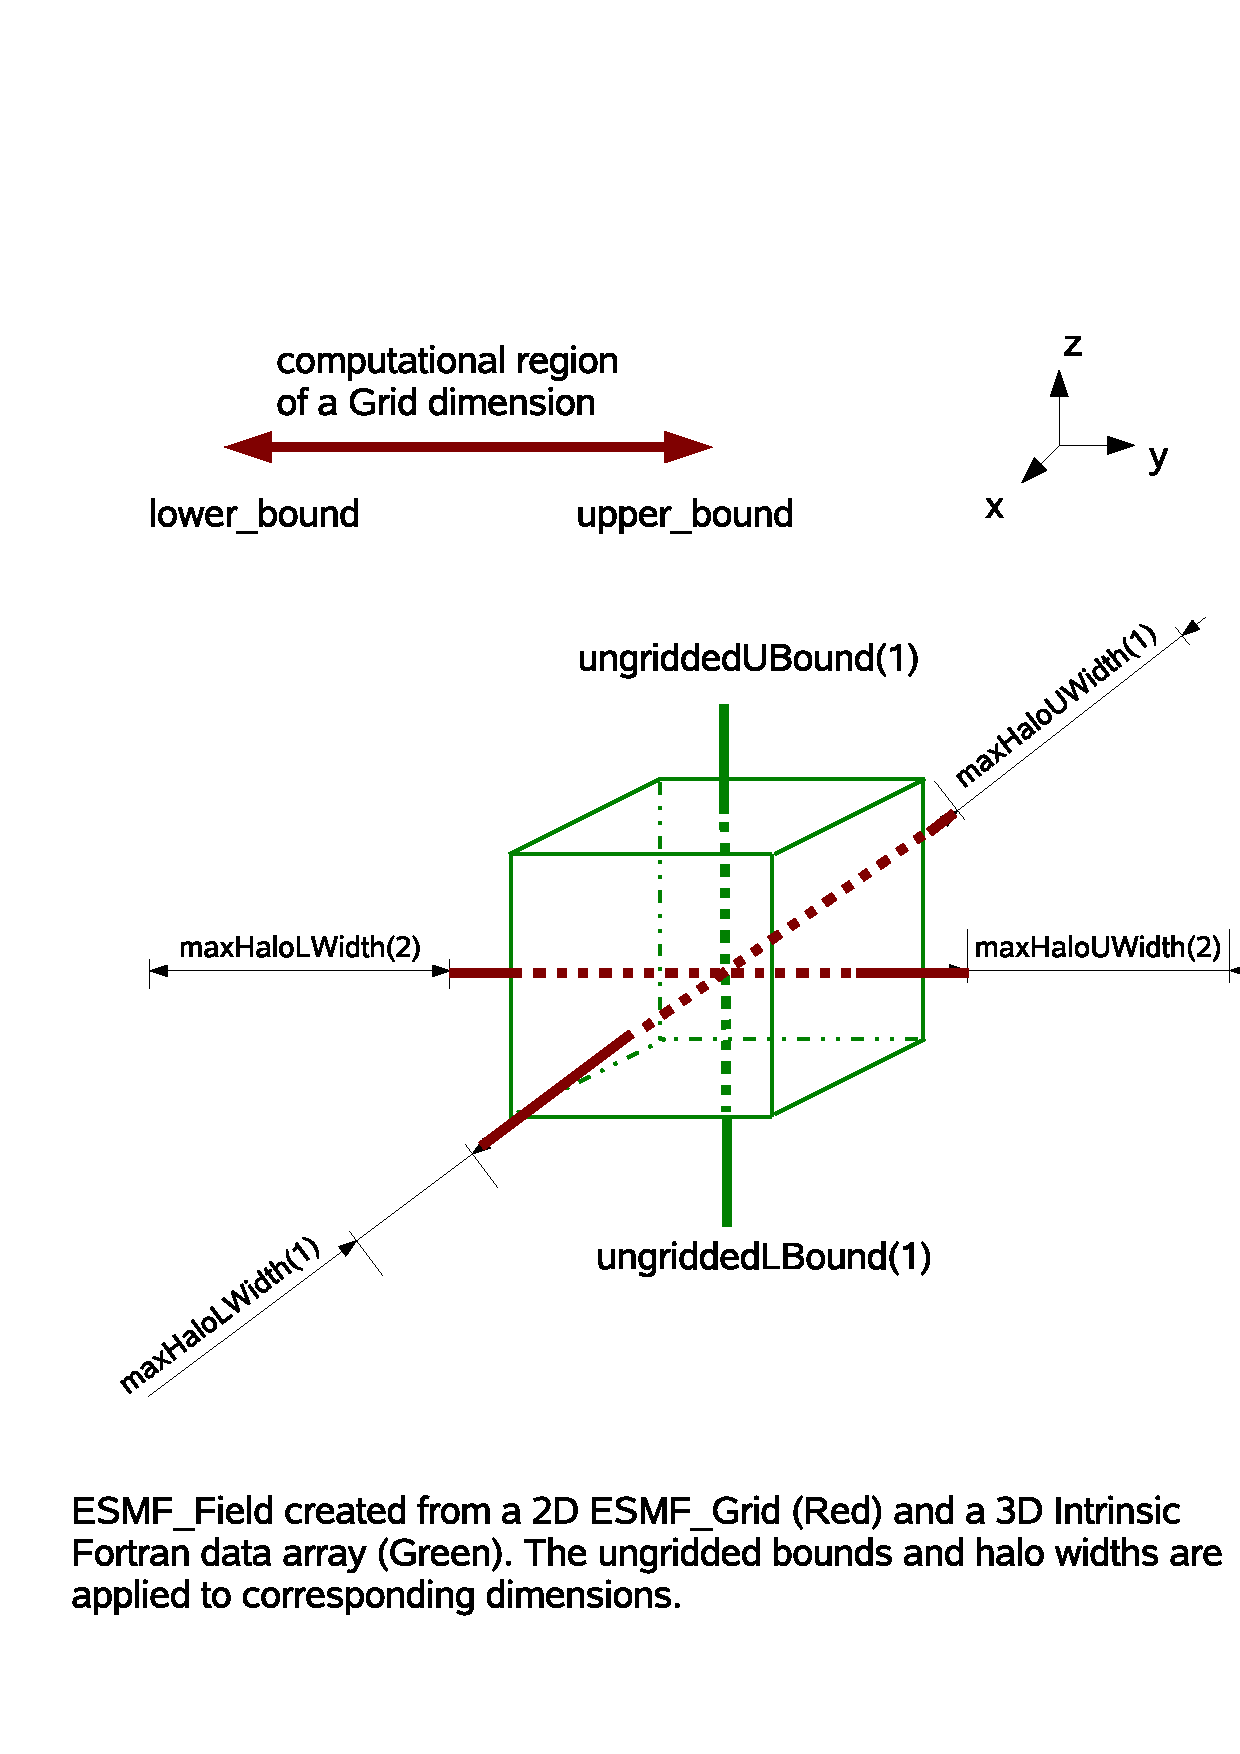
\includegraphics{FieldParameterSetup}}
  \caption{Field dimension configuration from Grid, halos, and Fortran data array.}
  \label{fig:fieldparameter}
  \end{figure}
  \end{center}
    
    The {\tt ESMF\_FieldCreate()} interface supports creating a Field from a Grid and a
    Fortran array padded with halos on the distributed dimensions of the Fortran
    array. Using this technique one can avoid passing non-contiguous Fortran array
    slice to FieldCreate. It guarantees the same exclusive region,
    and by using halos, it also defines a bigger total region to contain 
    the entire contiguous memory block of the Fortran array.
  
    The elements of totalLWidth and totalUWidth are applied in the order
    distributed dimensions appear in the Fortran array. By definition, 
    totalLWidth and totalUWidth are 1 dimensional arrays of non-negative 
    integer values. The size of haloWidth arrays is equal to the number of distributed
    dimensions of the Fortran array, which is also equal to the number of
    distributed dimensions of the Grid used in the Field creation.
  
    Because the order of totalWidth (representing both totalLWidth and
    totalUWidth) element is applied to the order distributed dimensions
    appear in the Fortran array dimensions, it's quite simple to compute
    the shape of distributed dimensions of the Fortran array. They are done
    in a similar manner when applying ungriddedLBound and ungriddedUBound 
    to ungridded dimensions of the Fortran array defined by rule 2.
  
    Assume we have the mapping from the dimension index of totalWidth
    to the dimension index of Fortran array, called mhw2fa; and we also
    have the mapping from dimension index of Fortran array to dimension
    index of the Grid, called fa2g. The shape of
    distributed dimensions of a Fortran array can be computed by rule 4: 
   
    \begin{verbatim}
  
    (4) fa_shape(mhw2fa(k)) = exclusiveCount(fa2g(mhw2fa(k)) + 
                              totalUWidth(k) + totalLWidth(k)
                          k = 1...size(totalWidth) 
  
    \end{verbatim}
    
    This rule may seem confusing but algorithmically the computation
    can be done by the following pseudocode:
  
    \begin{verbatim}
  
    fa_index = 1
    do i = 1, farray_rank
       if i-th dimension of Fortran array is distributed
           fa_shape(i) = exclusiveCount(fa2g(i)) + 
                         totalUWidth(fa_index) + totalLWidth(fa_index)
           fa_index = fa_index + 1
       endif
    enddo
  
    \end{verbatim}
  
    The only complication then is to figure out the mapping from Fortran
    array dimension index to Grid dimension index. This process can
    be done by computing the reverse mapping from Field to Grid.
  
    Typically, we don't have to consider these complications if the following
    conditions are met: 1) All Grid dimensions are distributed. 2) DistGrid
    in the Grid has a dimension index mapping to the Grid in the form of 
    natural order (/1,2,3,.../). This natural order mapping is the
    default mapping between various objects throughout ESMF. 3) Grid to Field
    mapping is in the form of natural order, i.e. default mapping. These
    seem like a lot of conditions but they are the default case in the interaction
    among DistGrid, Grid, and Field. When these conditions are met, which
    is typically true, the shape of distributed dimensions of Fortran array
    follows rule 5 in a simple form:
  
    \begin{verbatim}
  
    (5) fa_shape(k) = exclusiveCount(k) + 
                      totalUWidth(k) + totalLWidth(k) 
                  k = 1...size(totalWidth)
  
    \end{verbatim}
  
    Let's examine an example on how to apply rule 5. Suppose we have a
    5D array and a 3D Grid that has its first 3 dimensions mapped to the first
    3 dimensions of the Fortran array. totalLWidth=(/1,2,3/), 
    totalUWidth=(/7,9,10/), then by rule 5, the following pseudo code
    can be used to compute the shape of the first 3 dimensions of the Fortran
    array. The shape of the remaining two ungridded dimensions can be
    computed according to rule 2.
  
    \begin{verbatim}
  
    do k = 1, 3
        fa_shape(k) = exclusiveCount(k) + 
                      totalUWidth(k) + totalLWidth(k)) 
    enddo
  
    \end{verbatim}
  
    Suppose now gridToFieldMap=(/2,3,4/) instead which says
    the first dimension of Grid maps to the 2nd dimension of Field (or 
    Fortran array) and so on and so forth, we can obtain a more general form 
    of rule 5 by introducing first\_distdim\_index shift when Grid to Field
    map (gridToFieldMap) is in the form of (/a,a+1,a+2.../).
  
    \begin{verbatim}
  
    (6) fa_shape(k+first_distdim_index-1) = exclusiveCount(k) +
                                            totalUWidth(k) + totalLWidth(k)
                                        k = 1...size(totalWidth)
  
    \end{verbatim}
  
    It's obvious that first\_distdim\_index=a. If the first dimension of the Fortran
    array is distributed, then rule 6 degenerates into rule 5, which is
    the typical case.
  
    Back to our example creating a 3D Field from a 2D Grid and a 3D intrinsic
    Fortran array, we will use the Grid created from previous example
    that satisfies condition 1 and 2. We'll also use a simple gridToFieldMap
    (1,2) which is the default mapping that satisfies condition 3. 
    First we use rule 5 to compute
    the shape of distributed dimensions then we use rule 2 to compute the shape
    of the ungridded dimensions. 
%/////////////////////////////////////////////////////////////

 \begin{verbatim}
    gridToFieldMap2d(1) = 1
    gridToFieldMap2d(2) = 2
    totalLWidth2d(1) = 3
    totalLWidth2d(2) = 4
    totalUWidth2d(1) = 3
    totalUWidth2d(2) = 5
    do k = 1, 2
        fa_shape(k) = gec(k) + totalLWidth2d(k) + totalUWidth2d(k)
    end do
    fa_shape(3) = 7          ! 9-3+1
    allocate(farray3d(fa_shape(1), fa_shape(2), fa_shape(3)))
    field = ESMF_FieldCreate(grid, farray3d, ESMF_INDEX_DELOCAL, &
        ungriddedLBound=(/3/), ungriddedUBound=(/9/), &
        totalLWidth=totalLWidth2d, totalUWidth=totalUWidth2d, &
        gridToFieldMap=gridToFieldMap2d, &
        rc=rc)
    if (rc /= ESMF_SUCCESS) call ESMF_Finalize(endflag=ESMF_END_ABORT)
 
\end{verbatim}
 
%/////////////////////////////////////////////////////////////

  \subsubsection{Create a Field from a LocStream, typekind, and rank}
  \label{sec:field:usage:create_locs_tkr}
   
   In this example, an {\tt ESMF\_Field} is created from an {\tt ESMF\_LocStream} 
   and typekind/rank.
   The location stream object is uniformly distributed
   in a 1 dimensional space on 4 DEs. The rank is 1 dimensional. 
   Please refer to LocStream examples section for more information on LocStream creation.
   
%/////////////////////////////////////////////////////////////

 \begin{verbatim}

    locs = ESMF_LocStreamCreate(minIndex=1, maxIndex=16, rc=rc)
    if (rc /= ESMF_SUCCESS) call ESMF_Finalize(endflag=ESMF_END_ABORT)

    field = ESMF_FieldCreate(locs, typekind=ESMF_TYPEKIND_I4, &
        rc=rc)
    if (rc /= ESMF_SUCCESS) call ESMF_Finalize(endflag=ESMF_END_ABORT)

 
\end{verbatim}
 
%/////////////////////////////////////////////////////////////

  \subsubsection{Create a Field from a LocStream and arrayspec}
  \label{sec:field:usage:create_locs_arrayspec}
   
   In this example, an {\tt ESMF\_Field} is created from an {\tt ESMF\_LocStream} 
   and an {\tt ESMF\_Arrayspec}.
   The location stream object is uniformly distributed
   in a 1 dimensional space on 4 DEs. The arrayspec is 1 dimensional. 
   Please refer to LocStream examples section for more information on LocStream creation.
   
%/////////////////////////////////////////////////////////////

 \begin{verbatim}

    locs = ESMF_LocStreamCreate(minIndex=1, maxIndex=16, rc=rc)
    if (rc /= ESMF_SUCCESS) call ESMF_Finalize(endflag=ESMF_END_ABORT)

    call ESMF_ArraySpecSet(arrayspec, 1, ESMF_TYPEKIND_I4, rc=rc)
    if (rc /= ESMF_SUCCESS) call ESMF_Finalize(endflag=ESMF_END_ABORT)

    field = ESMF_FieldCreate(locs, arrayspec, &
        rc=rc)
    if (rc /= ESMF_SUCCESS) call ESMF_Finalize(endflag=ESMF_END_ABORT)

 
\end{verbatim}
 
%/////////////////////////////////////////////////////////////

  \subsubsection{Create a Field from a Mesh, typekind, and rank}
  \label{sec:field:usage:create_mesh_tkr}
   
   In this example, an {\tt ESMF\_Field} is created from an {\tt ESMF\_Mesh} 
   and typekind/rank.
   The mesh object is on a Euclidean surface that is partitioned to a 2x2 rectangular
   space with 4 elements and 9 nodes. The nodal space is represented by
   a distgrid with 9 indices. A Field is created on locally owned nodes on each PET.
   Therefore, the created Field has 9 data points globally.
   The mesh object can be represented by the picture
   below. For more information on Mesh creation, please see Section~\ref{sec:mesh:usage:meshCreation}.
   \begin{verbatim}
                Mesh Ids
  
    2.0   7 ------- 8 -------- 9
          |         |          |
          |    3    |    4     |
          |         |          |
    1.0   4 ------- 5 -------- 6
          |         |          |
          |    1    |    2     |
          |         |          |
    0.0   1 ------- 2 -------- 3
  
         0.0       1.0        2.0 
  
        Node Ids at corners
        Element Ids in centers
   
  
               Mesh Owners
  
    2.0   2 ------- 2 -------- 3
          |         |          |
          |    2    |    3     |
          |         |          |
    1.0   0 ------- 0 -------- 1
          |         |          |
          |    0    |    1     |
          |         |          |
    0.0   0 ------- 0 -------- 1
  
         0.0       1.0        2.0 
  
        Node Owners at corners
        Element Owners in centers
  \end{verbatim} 
   
%/////////////////////////////////////////////////////////////

 \begin{verbatim}
      ! Create Mesh structure in 1 step
      mesh=ESMF_MeshCreate(parametricDim=2,spatialDim=2, &
             nodeIds=nodeIds, nodeCoords=nodeCoords, &
             nodeOwners=nodeOwners, elementIds=elemIds,&
             elementTypes=elemTypes, elementConn=elemConn, &
             rc=rc)
      if (rc /= ESMF_SUCCESS) call ESMF_Finalize(endflag=ESMF_END_ABORT)

      ! Field is created on the 1 dimensional nodal distgrid. On
      ! each PET, Field is created on the locally owned nodes.
      field = ESMF_FieldCreate(mesh, typekind=ESMF_TYPEKIND_I4, rc=rc)
      if (rc /= ESMF_SUCCESS) call ESMF_Finalize(endflag=ESMF_END_ABORT)
 
\end{verbatim}
 
%/////////////////////////////////////////////////////////////

  \subsubsection{Create a Field from a Mesh and arrayspec}
  \label{sec:field:usage:create_mesh_arrayspec}
   
   In this example, an {\tt ESMF\_Field} is created from an {\tt ESMF\_Mesh} 
   and an {\tt ESMF\_Arrayspec}.
   The mesh object is on a Euclidean surface that is partitioned to a 2x2 rectangular
   space with 4 elements and 9 nodes. The nodal space is represented by
   a distgrid with 9 indices. Field is created on locally owned nodes on each PET.
   Therefore, the created Field has 9 data points globally.
   The mesh object can be represented by the picture
   below. For more information on Mesh creation, please see Section~\ref{sec:mesh:usage:meshCreation}.
   
%/////////////////////////////////////////////////////////////

 \begin{verbatim}
      ! Create Mesh structure in 1 step
      mesh=ESMF_MeshCreate(parametricDim=2,spatialDim=2, &
             nodeIds=nodeIds, nodeCoords=nodeCoords, &
             nodeOwners=nodeOwners, elementIds=elemIds,&
             elementTypes=elemTypes, elementConn=elemConn, &
             rc=rc)
      if (rc /= ESMF_SUCCESS) call ESMF_Finalize(endflag=ESMF_END_ABORT)

      call ESMF_ArraySpecSet(arrayspec, 1, ESMF_TYPEKIND_I4, rc=rc)
      if (rc /= ESMF_SUCCESS) call ESMF_Finalize(endflag=ESMF_END_ABORT)

      ! Field is created on the 1 dimensional nodal distgrid. On
      ! each PET, Field is created on the locally owned nodes.
      field = ESMF_FieldCreate(mesh, arrayspec, rc=rc)
      if (rc /= ESMF_SUCCESS) call ESMF_Finalize(endflag=ESMF_END_ABORT)
 
\end{verbatim}
 
%/////////////////////////////////////////////////////////////

  \subsubsection{Create a Field from a Mesh and an Array}
  \label{sec:field:usage:create_mesh_array}
   
   In this example, an {\tt ESMF\_Field} is created from an {\tt ESMF\_Mesh} 
   and an {\tt ESMF\_Array}. The mesh object is created in the previous example and
   the array object is retrieved from the field created in the previous example too.
   
%/////////////////////////////////////////////////////////////

 \begin{verbatim}
    call ESMF_MeshGet(mesh, nodalDistgrid=distgrid, rc=rc)
    if (rc /= ESMF_SUCCESS) call ESMF_Finalize(endflag=ESMF_END_ABORT)
    array = ESMF_ArrayCreate(distgrid=distgrid, arrayspec=arrayspec, rc=rc)
    if (rc /= ESMF_SUCCESS) call ESMF_Finalize(endflag=ESMF_END_ABORT)
    ! query the array from the previous example
    call ESMF_FieldGet(field, array=array, rc=rc)
    if (rc /= ESMF_SUCCESS) call ESMF_Finalize(endflag=ESMF_END_ABORT)
    ! create a Field from a mesh and an array
    field1 = ESMF_FieldCreate(mesh, array, rc=rc)
    if (rc /= ESMF_SUCCESS) call ESMF_Finalize(endflag=ESMF_END_ABORT)
 
\end{verbatim}
 
%/////////////////////////////////////////////////////////////

  \subsubsection{Create a Field from a Mesh and an ArraySpec with optional features}
  \label{sec:field:usage:createMeshArrayspecOpt}
  
   In this example, an {\tt ESMF\_Field} is created from an {\tt ESMF\_Mesh}
   and an {\tt ESMF\_ArraySpec}. The mesh object is created in the previous example.
   The Field is also created with optional arguments such as ungridded dimensions
   and dimension mapping.
  
   In this example, the mesh is mapped to the 2nd dimension of the
   {\tt ESMF\_Field}, with its first dimension being the ungridded dimension with bounds 1,3.
   
%/////////////////////////////////////////////////////////////

 \begin{verbatim}
    call ESMF_ArraySpecSet(arrayspec, 2, ESMF_TYPEKIND_I4, rc=rc)
    field = ESMF_FieldCreate(mesh, arrayspec=arrayspec, gridToFieldMap=(/2/), &
        ungriddedLBound=(/1/), ungriddedUBound=(/3/), rc=rc)
    if (rc /= ESMF_SUCCESS) call ESMF_Finalize(endflag=ESMF_END_ABORT)
 
\end{verbatim}

%...............................................................
\setlength{\parskip}{\oldparskip}
\setlength{\parindent}{\oldparindent}
\setlength{\baselineskip}{\oldbaselineskip}

%%                **** IMPORTANT NOTICE *****
% This LaTeX file has been automatically produced by ProTeX v. 1.1
% Any changes made to this file will likely be lost next time
% this file is regenerated from its source. Send questions 
% to Arlindo da Silva, dasilva@gsfc.nasa.gov
 
\setlength{\oldparskip}{\parskip}
\setlength{\parskip}{1.5ex}
\setlength{\oldparindent}{\parindent}
\setlength{\parindent}{0pt}
\setlength{\oldbaselineskip}{\baselineskip}
\setlength{\baselineskip}{11pt}
 
%--------------------- SHORT-HAND MACROS ----------------------
\def\bv{\begin{verbatim}}
\def\ev{\end{verbatim}}
\def\be{\begin{equation}}
\def\ee{\end{equation}}
\def\bea{\begin{eqnarray}}
\def\eea{\end{eqnarray}}
\def\bi{\begin{itemize}}
\def\ei{\end{itemize}}
\def\bn{\begin{enumerate}}
\def\en{\end{enumerate}}
\def\bd{\begin{description}}
\def\ed{\end{description}}
\def\({\left (}
\def\){\right )}
\def\[{\left [}
\def\]{\right ]}
\def\<{\left  \langle}
\def\>{\right \rangle}
\def\cI{{\cal I}}
\def\diag{\mathop{\rm diag}}
\def\tr{\mathop{\rm tr}}
%-------------------------------------------------------------

\markboth{Left}{Source File: ESMF\_FieldRepDimEx.F90,  Date: Tue May  5 21:00:02 MDT 2020
}

 
%/////////////////////////////////////////////////////////////

  \subsubsection{Create a Field with replicated dimensions}
  \label{sec:field:usage:create_repdim}
  
    \begin{sloppypar}
    In this example an {\tt ESMF\_Field} with replicated dimension is created from an {\tt ESMF\_Grid} and
    an {\tt ESMF\_Arrayspec}. A user can also use other {\tt ESMF\_FieldCreate()} methods to create replicated
    dimension Field, this example illustrates the key concepts and use of a replicated dimension Field.
    \end{sloppypar}
  
    Normally gridToFieldMap argument in {\tt ESMF\_FieldCreate()} should not contain
    0 value entries. However, for a Field with replicated dimension, a 0 entry in gridToFieldMap
    indicates the corresponding Grid dimension is replicated in the Field. In such a Field,
    the rank of the Field is no longer necessarily greater than its Grid rank.
    An example will make this clear. We will start by creating Distgrid and Grid.
   
%/////////////////////////////////////////////////////////////

 \begin{verbatim}
    ! create 4D distgrid
    distgrid = ESMF_DistGridCreate(minIndex=(/1,1,1,1/), &
        maxIndex=(/6,4,6,4/), regDecomp=(/2,1,2,1/), rc=rc)
    if (rc /= ESMF_SUCCESS) call ESMF_Finalize(endflag=ESMF_END_ABORT)

    ! create 4D grid on top of the 4D distgrid
    grid = ESMF_GridCreate(distgrid=distgrid, name="grid", rc=rc)
    if (rc /= ESMF_SUCCESS) call ESMF_Finalize(endflag=ESMF_END_ABORT)

    ! create 3D arrayspec
    call ESMF_ArraySpecSet(arrayspec, 3, ESMF_TYPEKIND_R8, rc=rc)
    if (rc /= ESMF_SUCCESS) call ESMF_Finalize(endflag=ESMF_END_ABORT)
 
\end{verbatim}
 
%/////////////////////////////////////////////////////////////

   In this example, a user creates a 3D Field with replicated dimension
   replicated along the 2nd and 4th dimension of its underlying 4D Grid.
   In addition, the 2nd dimension of the Field is ungridded (why?). The 1st and
   3rd dimensions of the Field have halos. 
%/////////////////////////////////////////////////////////////

 \begin{verbatim}
    ! create field, 2nd and 4th dimensions of the Grid are replicated
    field = ESMF_FieldCreate(grid, arrayspec, indexflag=ESMF_INDEX_DELOCAL, &
        gridToFieldMap=(/1,0,2,0/), &
        ungriddedLBound=(/1/), ungriddedUBound=(/4/), &
        totalLWidth=(/1,1/), totalUWidth=(/4,5/), &
        staggerloc=ESMF_STAGGERLOC_CORNER, &
        rc=rc)
    if (rc /= ESMF_SUCCESS) call ESMF_Finalize(endflag=ESMF_END_ABORT)

    ! get basic information from the field
    call ESMF_FieldGet(field, grid=grid1, array=array, typekind=typekind, &
        dimCount=dimCount, staggerloc=lstaggerloc, &
        gridToFieldMap=lgridToFieldMap, ungriddedLBound=lungriddedLBound, &
        ungriddedUBound=lungriddedUBound, totalLWidth=ltotalLWidth, &
        totalUWidth=ltotalUWidth, rc=rc)
    if (rc /= ESMF_SUCCESS) call ESMF_Finalize(endflag=ESMF_END_ABORT)

    ! get bounds information from the field
    call ESMF_FieldGet(field, localDe=0, farrayPtr=farray, &
        exclusiveLBound=felb, exclusiveUBound=feub, exclusiveCount=fec, &
        computationalLBound=fclb, computationalUBound=fcub, &
        computationalCount=fcc, totalLBound=ftlb, totalUBound=ftub, &
        totalCount=ftc, rc=rc)
    if (rc /= ESMF_SUCCESS) call ESMF_Finalize(endflag=ESMF_END_ABORT)

 
\end{verbatim}
 
%/////////////////////////////////////////////////////////////

   Next we verify that the field and array bounds agree with each other 
%/////////////////////////////////////////////////////////////

 \begin{verbatim}
    call ESMF_ArrayGet(array, rank=arank, dimCount=adimCount, rc=rc)
    if (rc /= ESMF_SUCCESS) call ESMF_Finalize(endflag=ESMF_END_ABORT)

    gridrank_repdim = 0
    do i = 1, size(gridToFieldMap)
        if(gridToFieldMap(i) == 0) gridrank_repdim = gridrank_repdim + 1
    enddo
 
\end{verbatim}
 
%/////////////////////////////////////////////////////////////

   Number of undistributed dimension of the array {\it X} is computed from
   total rank of the array {\it A}, the dimension count of its underlying distgrid
   {\it B} and number of replicated dimension in the distgrid {\it C}.
   We have the following formula: X = A - (B - C) 
%/////////////////////////////////////////////////////////////

 \begin{verbatim}
    allocate(audlb(arank-adimCount+gridrank_repdim), &
        audub(arank-adimCount+gridrank_repdim))
    call ESMF_ArrayGet(array, exclusiveLBound=aelb, exclusiveUBound=aeub, &
        computationalLBound=aclb, computationalUBound=acub, &
        totalLBound=atlb, totalUBound=atub, &
        undistLBound=audlb, undistUBound=audub, &
        rc=rc)
    if (rc /= ESMF_SUCCESS) call ESMF_Finalize(endflag=ESMF_END_ABORT)

    ! verify the ungridded bounds from field match
    ! undistributed bounds from its underlying array
    do i = 1, arank-adimCount
        if(lungriddedLBound(i) .ne. audlb(i) ) &
            rc = ESMF_FAILURE
    enddo
    if (rc /= ESMF_SUCCESS) call ESMF_Finalize(endflag=ESMF_END_ABORT)

    do i = 1, arank-adimCount
        if(lungriddedUBound(i) .ne. audub(i) ) &
            rc = ESMF_FAILURE
    enddo
    if (rc /= ESMF_SUCCESS) call ESMF_Finalize(endflag=ESMF_END_ABORT)
 
\end{verbatim}
 
%/////////////////////////////////////////////////////////////

   We then verify the data in the replicated dimension Field can be updated and accessed. 
%/////////////////////////////////////////////////////////////

 \begin{verbatim}
    do ik = ftlb(3), ftub(3)
     do ij = ftlb(2), ftub(2)
      do ii = ftlb(1), ftub(1)
        farray(ii,ij,ik) = ii+ij*2+ik
      enddo
     enddo
    enddo
    ! access and verify
    call ESMF_FieldGet(field, localDe=0, farrayPtr=farray1, &
        rc=rc)
    if (rc /= ESMF_SUCCESS) call ESMF_Finalize(endflag=ESMF_END_ABORT)
    do ik = ftlb(3), ftub(3)
     do ij = ftlb(2), ftub(2)
      do ii = ftlb(1), ftub(1)
        n = ii+ij*2+ik
        if(farray1(ii,ij,ik) .ne. n ) rc = ESMF_FAILURE
      enddo
     enddo
    enddo
    if (rc /= ESMF_SUCCESS) call ESMF_Finalize(endflag=ESMF_END_ABORT)

    ! release resources
    call ESMF_FieldDestroy(field)
    call ESMF_GridDestroy(grid)
    call ESMF_DistGridDestroy(distgrid)
 
\end{verbatim}

%...............................................................
\setlength{\parskip}{\oldparskip}
\setlength{\parindent}{\oldparindent}
\setlength{\baselineskip}{\oldbaselineskip}

%%                **** IMPORTANT NOTICE *****
% This LaTeX file has been automatically produced by ProTeX v. 1.1
% Any changes made to this file will likely be lost next time
% this file is regenerated from its source. Send questions 
% to Arlindo da Silva, dasilva@gsfc.nasa.gov
 
\setlength{\oldparskip}{\parskip}
\setlength{\parskip}{1.5ex}
\setlength{\oldparindent}{\parindent}
\setlength{\parindent}{0pt}
\setlength{\oldbaselineskip}{\baselineskip}
\setlength{\baselineskip}{11pt}
 
%--------------------- SHORT-HAND MACROS ----------------------
\def\bv{\begin{verbatim}}
\def\ev{\end{verbatim}}
\def\be{\begin{equation}}
\def\ee{\end{equation}}
\def\bea{\begin{eqnarray}}
\def\eea{\end{eqnarray}}
\def\bi{\begin{itemize}}
\def\ei{\end{itemize}}
\def\bn{\begin{enumerate}}
\def\en{\end{enumerate}}
\def\bd{\begin{description}}
\def\ed{\end{description}}
\def\({\left (}
\def\){\right )}
\def\[{\left [}
\def\]{\right ]}
\def\<{\left  \langle}
\def\>{\right \rangle}
\def\cI{{\cal I}}
\def\diag{\mathop{\rm diag}}
\def\tr{\mathop{\rm tr}}
%-------------------------------------------------------------

\markboth{Left}{Source File: ESMF\_FieldArbGridEx.F90,  Date: Tue May  5 21:00:02 MDT 2020
}

 
%/////////////////////////////////////////////////////////////

  \subsubsection{Create a Field on an arbitrarily distributed Grid}
  \label{sec:field:usage:createArbGrid}
  
    With the introduction of Field on arbitrarily distributed Grid, Field has two kinds of dimension
    count: one associated geometrical (or physical) dimensionality, the other one associated with its
    memory index space representation. Field and Grid dimCount reflect the physical index 
    space of the objects. A new type of dimCount rank should be added to both of these entities.
    The rank gives the number of dimensions of the memory index space of the objects.
    This would be the dimension of the pointer pulled out of Field and the
    size of the bounds vector, for example. 
  
    For non-arbitrary Grids rank=dimCount, but for grids and fields with
    arbitrary dimensions rank = dimCount - (number of Arb dims) + 1
    (Internally Field can use the Arb info from the grid to create the mapping
    from the Field Array to the DistGrid)
  
    When creating a Field size(GridToFieldMap)=dimCount for both Arb and Non-arb grids
    This array specifies the mapping of Field to Grid identically for both Arb and Nonarb grids 
    If a zero occurs in an entry corresponding to any arbitrary dimension, then
    a zero must occur in every entry corresponding to an arbitrary dimension (i.e.
    all arbitrary dimensions must either be all replicated or all not replicated,
    they can't be broken apart).
  
    In this example an {\tt ESMF\_Field} is created from an arbitrarily distributed {\tt ESMF\_Grid} and 
    an {\tt ESMF\_Arrayspec}. A user can also use other {\tt ESMF\_FieldCreate()} methods to create 
    such a Field, this example illustrates the key concepts and use of Field on arbitrary distributed Grid.
    
    The Grid is 3 dimensional in physics index space but the first two dimension are collapsed into
    a single memory index space. Thus the resulting Field is 3D in physics index space and 2D in memory index
    space. This is made obvious with the 2D arrayspec used to create this Field.
   
%/////////////////////////////////////////////////////////////

 \begin{verbatim}
    ! create a 3D grid with the first 2 dimensions collapsed 
    ! and arbitrarily distributed
    grid3d = ESMF_GridCreateNoPeriDim(coordTypeKind=ESMF_TYPEKIND_R8, &
      minIndex=(/1,1,1/), maxIndex=(/xdim, ydim,zdim/), &
      arbIndexList=localArbIndex,arbIndexCount=localArbIndexCount, &
      name="arb3dgrid", rc=rc)
    if (rc /= ESMF_SUCCESS) call ESMF_Finalize(endflag=ESMF_END_ABORT)

    ! create a 2D arrayspec
    call ESMF_ArraySpecSet(arrayspec2D, rank=2, typekind=ESMF_TYPEKIND_R4, &
         rc=rc)
    if (rc /= ESMF_SUCCESS) call ESMF_Finalize(endflag=ESMF_END_ABORT)

    ! create a 2D Field using the Grid and the arrayspec
    field = ESMF_FieldCreate(grid3d, arrayspec2D, rc=rc)
    if (rc /= ESMF_SUCCESS) call ESMF_Finalize(endflag=ESMF_END_ABORT)
  
    call ESMF_FieldGet(field, rank=rank, dimCount=dimCount, &
                       rc=rc)
    if (myPet .eq. 0) print *, 'Field rank, dimCount', &
                                rank, dimCount
    if (rc /= ESMF_SUCCESS) call ESMF_Finalize(endflag=ESMF_END_ABORT)
  
    ! verify that the dimension counts are correct
    if (rank .ne. 2) correct = .false.
    if (dimCount .ne. 3) correct = .false.  
 
\end{verbatim}
 
%/////////////////////////////////////////////////////////////

  \subsubsection{Create a Field on an arbitrarily distributed Grid with replicated dimensions \& ungridded bounds}
  \label{sec:field:usage:createArbGridRep}
  
    The next example is slightly more complicated in
    that the Field also contains one ungridded dimension and its gridded dimension
    is replicated on the arbitrarily distributed dimension of the Grid.
   
    The same 3D Grid and 2D arrayspec in the previous example
    are used but a gridToFieldMap argument
    is supplied to the {\tt ESMF\_FieldCreate()} call. The first 2 entries of
    the map are 0, the last (3rd) entry is 1. The 3rd dimension of the Grid is
    mapped to the first dimension of the Field, this dimension is then replicated
    on the arbitrarily distributed dimensions of the Grid. In addition, the
    Field also has one ungridded dimension. Thus the final dimension count of the
    Field is 2 in both physics and memory index space.
   
%/////////////////////////////////////////////////////////////

 \begin{verbatim}
    field = ESMF_FieldCreate(grid3d, arrayspec2D,gridToFieldMap=(/0,0,1/), &
            ungriddedLBound=(/1/), ungriddedUBound=(/10/),rc=rc)
    if (rc /= ESMF_SUCCESS) call ESMF_Finalize(endflag=ESMF_END_ABORT)
  
    call ESMF_FieldGet(field, rank=rank, dimCount=dimCount, &
                       rc=rc)
    if (myPet .eq. 0) print *, 'Field rank, dimCount', &
                                rank, dimCount
    if (rc /= ESMF_SUCCESS) call ESMF_Finalize(endflag=ESMF_END_ABORT)
  
    if (rank .ne. 2) correct = .false.
    if (dimCount .ne. 2) correct = .false.  
 
\end{verbatim}

%...............................................................
\setlength{\parskip}{\oldparskip}
\setlength{\parindent}{\oldparindent}
\setlength{\baselineskip}{\oldbaselineskip}

%%\input{../Infrastructure/Field/doc/ESMF_FieldGetEx_fapi}
%%\input{../Infrastructure/Field/doc/ESMF_FieldSetEx_fapi}
%%                **** IMPORTANT NOTICE *****
% This LaTeX file has been automatically produced by ProTeX v. 1.1
% Any changes made to this file will likely be lost next time
% this file is regenerated from its source. Send questions 
% to Arlindo da Silva, dasilva@gsfc.nasa.gov
 
\setlength{\oldparskip}{\parskip}
\setlength{\parskip}{1.5ex}
\setlength{\oldparindent}{\parindent}
\setlength{\parindent}{0pt}
\setlength{\oldbaselineskip}{\baselineskip}
\setlength{\baselineskip}{11pt}
 
%--------------------- SHORT-HAND MACROS ----------------------
\def\bv{\begin{verbatim}}
\def\ev{\end{verbatim}}
\def\be{\begin{equation}}
\def\ee{\end{equation}}
\def\bea{\begin{eqnarray}}
\def\eea{\end{eqnarray}}
\def\bi{\begin{itemize}}
\def\ei{\end{itemize}}
\def\bn{\begin{enumerate}}
\def\en{\end{enumerate}}
\def\bd{\begin{description}}
\def\ed{\end{description}}
\def\({\left (}
\def\){\right )}
\def\[{\left [}
\def\]{\right ]}
\def\<{\left  \langle}
\def\>{\right \rangle}
\def\cI{{\cal I}}
\def\diag{\mathop{\rm diag}}
\def\tr{\mathop{\rm tr}}
%-------------------------------------------------------------

\markboth{Left}{Source File: ESMF\_FieldRegridEx.F90,  Date: Tue May  5 21:00:02 MDT 2020
}

 
%/////////////////////////////////////////////////////////////

  \subsubsection{Field regridding}\label{sec:fieldregrid}
  
   This section describes the Field regrid methods. For an in depth description of ESMF regridding and the options available
   please see Section~\ref{sec:regrid}. 
  
   The basic flow of ESMF Field regridding is as follows. First a source and destination geometry object are created, depending on 
   the regrid method they can be either a Grid, a Mesh, or a LocStream. 
   Next Fields are built on the source and destination grid objects. These Fields are then passed into {\tt ESMF\_FieldRegridStore()}. The user can either get a 
   sparse matrix from this call and/or a {\tt routeHandle}. If the user gets the sparse matrix then they are responsible for deallocating it, but other than that
   can use it as they wish. The {\tt routeHandle} can be used in the {\tt ESMF\_FieldRegrid()} call to perform the actual interpolation of data from the source 
   to the destination field. This interpolation can be repeated for the same set of Fields as long as the coordinates at the staggerloc involved in the
   regridding in the associated grid object don't change. The same {\tt routeHandle} can also be used between any pair of Fields that matches the original 
   pari in {\em type}, {\em kind}, and memory layout of the {\em gridded} dimensions. However, the size, number, and index order of {\em ungridded} dimensions
   may be different. See section \ref{RH:Reusability} for a more detailed discussion of RouteHandle reusability.
   However, if you want                                     
   the routehandle to be the same interpolation between the grid objects upon which the Fields are built as was calculated                                        
   with the original {\tt ESMF\_FieldRegridStore()} call, then there                                                                                              
   are additional constraints on the grid objects. To be the same interpolation, the grid objects upon which the                                                  
   Fields are build must contain the same coordinates at the stagger locations involved in the regridding as                                                      
   the original source and destination Fields used in the {\tt ESMF\_FieldRegridStore()} call.                                                                    
   The routehandle represents the interpolation between the grid objects as they were during the {\tt ESMF\_FieldRegridStore()} call.                             
   So if the coordinates at the stagger location in the grid objects change, a new call to {\tt ESMF\_FieldRegridStore()}                                         
   is necessary to compute the interpolation between that new set of coordinates. When finished with the {\tt routeHandle} 
   {\tt ESMF\_FieldRegridRelease()} should be used to 
   free the associated memory. 
  
   The following example demonstrates doing a regrid operation between two Fields.
   
%/////////////////////////////////////////////////////////////

 \begin{verbatim}

  ! (Create source Grid, Mesh, or LocStream.)
  ! (Create srcField on the above.)

  ! (Create destination Grid, Mesh, or LocStream.)
  ! (Create dstField on the above.)
  
  ! Create the routeHandle which encodes the communication and
  ! information necessary for the regrid sparse matrix multiply.
  call ESMF_FieldRegridStore(srcField=srcField, dstField=dstField, &
                             routeHandle=routeHandle, rc=localrc)
 
\end{verbatim}
 
%/////////////////////////////////////////////////////////////

 \begin{verbatim}
 
  ! Can loop here regridding from srcField to dstField 
  ! do i=1,....

       ! (Put data into srcField)

       ! Use the routeHandle to regrid data from srcField to dstField.
       ! As described above, the same routeHandle can be used to 
       ! regrid a large class of different source and destination Fields. 
       call ESMF_FieldRegrid(srcField, dstField, routeHandle, rc=localrc)
 
\end{verbatim}
 
%/////////////////////////////////////////////////////////////

 \begin{verbatim}

  !    (Use data in dstField)

  ! enddo 


  ! Free the buffers and data associated with the routeHandle. 
  call ESMF_FieldRegridRelease(routeHandle, rc=localrc)

 
\end{verbatim}

%...............................................................
\setlength{\parskip}{\oldparskip}
\setlength{\parindent}{\oldparindent}
\setlength{\baselineskip}{\oldbaselineskip}

%%                **** IMPORTANT NOTICE *****
% This LaTeX file has been automatically produced by ProTeX v. 1.1
% Any changes made to this file will likely be lost next time
% this file is regenerated from its source. Send questions 
% to Arlindo da Silva, dasilva@gsfc.nasa.gov
 
\setlength{\oldparskip}{\parskip}
\setlength{\parskip}{1.5ex}
\setlength{\oldparindent}{\parindent}
\setlength{\parindent}{0pt}
\setlength{\oldbaselineskip}{\baselineskip}
\setlength{\baselineskip}{11pt}
 
%--------------------- SHORT-HAND MACROS ----------------------
\def\bv{\begin{verbatim}}
\def\ev{\end{verbatim}}
\def\be{\begin{equation}}
\def\ee{\end{equation}}
\def\bea{\begin{eqnarray}}
\def\eea{\end{eqnarray}}
\def\bi{\begin{itemize}}
\def\ei{\end{itemize}}
\def\bn{\begin{enumerate}}
\def\en{\end{enumerate}}
\def\bd{\begin{description}}
\def\ed{\end{description}}
\def\({\left (}
\def\){\right )}
\def\[{\left [}
\def\]{\right ]}
\def\<{\left  \langle}
\def\>{\right \rangle}
\def\cI{{\cal I}}
\def\diag{\mathop{\rm diag}}
\def\tr{\mathop{\rm tr}}
%-------------------------------------------------------------

\markboth{Left}{Source File: ESMF\_FieldRegridMaskEx.F90,  Date: Tue May  5 21:00:02 MDT 2020
}

 
%/////////////////////////////////////////////////////////////

  
  \subsubsection{Field regrid with masking}
   As before, to create the sparse matrix regrid operator we call the
   {\tt ESMF\_FieldRegridStore()} routine. 
   However, in this case we apply masking to the regrid operation. 
   The mask value for each index location in the Grids may be set using
   the {\tt ESMF\_GridAddItem()} call (see Section~\ref{sec:usage:items}
   and Section~\ref{sec:usage:items:accessing}). Mask values may be set independently 
   for the source and destination Grids. If no mask values have been set in a Grid, then it is 
   assumed no masking should be used for that Grid. The {\tt srcMaskValues}
   parameter allows the user to set the list of values which indicate
   that a source location should be masked out. The {\tt dstMaskValues}
   parameter allows the user to set the list of values which indicate
   that a destination location should be masked out. The absence of 
   one of these parameters indicates that no masking should be used
   for that Field (e.g no {\tt srcMaskValue} parameter indicates that source
   masking shouldn't occur). The {\tt unmappedaction} flag may be
   used with or without masking and indicates what should occur
   if destination points can not be mapped to a source cell. 
   Here the {\tt ESMF\_UNMAPPEDACTION\_IGNORE} value indicates that unmapped
   destination points are to be ignored and no sparse matrix entries should be
    generated for them.  
%/////////////////////////////////////////////////////////////

 \begin{verbatim}
  call ESMF_FieldRegridStore(srcField=srcField, srcMaskValues=(/1/),       &
                             dstField=dstField, dstMaskValues=(/1/),       &
                             unmappedaction=ESMF_UNMAPPEDACTION_IGNORE, &
                             routeHandle=routeHandle,                      &
                             regridmethod=ESMF_REGRIDMETHOD_BILINEAR,     &
                             rc=localrc)
 
\end{verbatim}
 
%/////////////////////////////////////////////////////////////

  
   The {\tt ESMF\_FieldRegrid} and {\tt ESMF\_FieldRegridRelease} calls
   may then be applied as in the previous example.
%...............................................................
\setlength{\parskip}{\oldparskip}
\setlength{\parindent}{\oldparindent}
\setlength{\baselineskip}{\oldbaselineskip}
 <
%%                **** IMPORTANT NOTICE *****
% This LaTeX file has been automatically produced by ProTeX v. 1.1
% Any changes made to this file will likely be lost next time
% this file is regenerated from its source. Send questions 
% to Arlindo da Silva, dasilva@gsfc.nasa.gov
 
\setlength{\oldparskip}{\parskip}
\setlength{\parskip}{1.5ex}
\setlength{\oldparindent}{\parindent}
\setlength{\parindent}{0pt}
\setlength{\oldbaselineskip}{\baselineskip}
\setlength{\baselineskip}{11pt}
 
%--------------------- SHORT-HAND MACROS ----------------------
\def\bv{\begin{verbatim}}
\def\ev{\end{verbatim}}
\def\be{\begin{equation}}
\def\ee{\end{equation}}
\def\bea{\begin{eqnarray}}
\def\eea{\end{eqnarray}}
\def\bi{\begin{itemize}}
\def\ei{\end{itemize}}
\def\bn{\begin{enumerate}}
\def\en{\end{enumerate}}
\def\bd{\begin{description}}
\def\ed{\end{description}}
\def\({\left (}
\def\){\right )}
\def\[{\left [}
\def\]{\right ]}
\def\<{\left  \langle}
\def\>{\right \rangle}
\def\cI{{\cal I}}
\def\diag{\mathop{\rm diag}}
\def\tr{\mathop{\rm tr}}
%-------------------------------------------------------------

\markboth{Left}{Source File: ESMF\_FieldCommEx.F90,  Date: Tue May  5 21:00:02 MDT 2020
}

 
%/////////////////////////////////////////////////////////////

   \subsubsection{Gather Field data onto root PET}
   \label{sec:field:usage:gather_2dptr}
  
   User can use {\tt ESMF\_FieldGather} interface to gather Field data from multiple
   PETs onto a single root PET. This interface is overloaded by type, kind, and rank.
  
   Note that the implementation of Scatter and Gather is not sequence index based.
   If the Field is built on arbitrarily distributed Grid, Mesh, LocStream or XGrid, 
   Gather will not gather data to rootPet 
   from source data points corresponding to the sequence index on the rootPet. 
   Instead Gather will gather a contiguous memory range from source PET to
   rootPet. The size of the memory range is equal to the number of 
   data elements on the source PET. Vice versa for the Scatter operation. 
   In this case, the user should use {\tt ESMF\_FieldRedist} to achieve
   the same data operation result. For examples how to use {\tt ESMF\_FieldRedist}
   to perform Gather and Scatter, please refer to
   \ref{sec:field:usage:redist_gathering} and
   \ref{sec:field:usage:redist_scattering}.
   
   In this example, we first create a 2D Field, then use {\tt ESMF\_FieldGather} to
   collect all the data in this Field into a data pointer on PET 0. 
%/////////////////////////////////////////////////////////////

 \begin{verbatim}
    ! Get current VM and pet number
    call ESMF_VMGetCurrent(vm, rc=rc)
    if (rc /= ESMF_SUCCESS) call ESMF_Finalize(endflag=ESMF_END_ABORT)

    call ESMF_VMGet(vm, localPet=lpe, rc=rc)
    if (rc /= ESMF_SUCCESS) call ESMF_Finalize(endflag=ESMF_END_ABORT)

    ! Create a 2D Grid and use this grid to create a Field
    ! farray is the Fortran data array that contains data on each PET.
    grid = ESMF_GridCreateNoPeriDim(minIndex=(/1,1/), maxIndex=(/10,20/), &
        regDecomp=(/2,2/), &
        name="grid", rc=rc)
    if (rc /= ESMF_SUCCESS) call ESMF_Finalize(endflag=ESMF_END_ABORT)

    field = ESMF_FieldCreate(grid, typekind=ESMF_TYPEKIND_I4, rc=localrc)
    if (localrc /= ESMF_SUCCESS) call ESMF_Finalize(endflag=ESMF_END_ABORT)


    call ESMF_FieldGet(field, farrayPtr=fptr, rc=localrc)
    if (localrc /= ESMF_SUCCESS) call ESMF_Finalize(endflag=ESMF_END_ABORT)
    !---------Initialize pet specific field data----------------
    !    1        5         10
    ! 1  +--------+---------+
    !    |        |         |
    !    |   0    |    1    |
    !    |        |         |
    ! 10 +--------+---------+
    !    |        |         |
    !    |   2    |    3    |
    !    |        |         |
    ! 20 +--------+---------+
    fptr = lpe

    ! allocate the Fortran data array on PET 0 to store gathered data
    if(lpe .eq. 0) then
      allocate (farrayDst(10,20))
    else
      allocate (farrayDst(0,0))
    end if
    call ESMF_FieldGather(field, farrayDst, rootPet=0, rc=rc)
    if (rc /= ESMF_SUCCESS) call ESMF_Finalize(endflag=ESMF_END_ABORT)

    ! check that the values gathered on rootPet are correct
    if(lpe .eq. 0) then
       do i = 1, 5
          do j = 1, 10
             if(farrayDst(i, j) .ne. 0) localrc=ESMF_FAILURE
          enddo
       enddo
      if (localrc /= ESMF_SUCCESS) call ESMF_Finalize(endflag=ESMF_END_ABORT)
       do i = 6, 10
          do j = 1, 10
             if(farrayDst(i, j) .ne. 1) localrc=ESMF_FAILURE
          enddo
       enddo
      if (localrc /= ESMF_SUCCESS) call ESMF_Finalize(endflag=ESMF_END_ABORT)
       do i = 1, 5
          do j = 11, 20
             if(farrayDst(i, j) .ne. 2) localrc=ESMF_FAILURE
          enddo
       enddo
      if (localrc /= ESMF_SUCCESS) call ESMF_Finalize(endflag=ESMF_END_ABORT)
       do i = 6, 10
          do j = 11, 20
             if(farrayDst(i, j) .ne. 3) localrc=ESMF_FAILURE
          enddo
       enddo
      if (localrc /= ESMF_SUCCESS) call ESMF_Finalize(endflag=ESMF_END_ABORT)
    endif

    ! destroy all objects created in this example to prevent memory leak
    call ESMF_FieldDestroy(field, rc=rc)
    if (rc /= ESMF_SUCCESS) call ESMF_Finalize(endflag=ESMF_END_ABORT)
    call ESMF_GridDestroy(grid, rc=rc)
    if (rc /= ESMF_SUCCESS) call ESMF_Finalize(endflag=ESMF_END_ABORT)
    if(lpe .eq. 0) deallocate(farrayDst)
 
\end{verbatim}
 
%/////////////////////////////////////////////////////////////

   \subsubsection{Scatter Field data from root PET onto its set of joint PETs}
   \label{sec:field:usage:scatter_2dptr}
  
   User can use {\tt ESMF\_FieldScatter} interface to scatter Field data from root
   PET onto its set of joint PETs. This interface is overloaded by type, kind, and rank.
   
   In this example, we first create a 2D Field, then use {\tt ESMF\_FieldScatter} to
   scatter the data from a data array located on PET 0 onto this Field. 
%/////////////////////////////////////////////////////////////

 \begin{verbatim}
    ! Create a 2D Grid and use this grid to create a Field
    ! farray is the Fortran data array that contains data on each PET.
    grid = ESMF_GridCreateNoPeriDim(minIndex=(/1,1/), maxIndex=(/10,20/), &
        regDecomp=(/2,2/), &
        name="grid", rc=rc)
    if (rc /= ESMF_SUCCESS) call ESMF_Finalize(endflag=ESMF_END_ABORT)

    field = ESMF_FieldCreate(grid, typekind=ESMF_TYPEKIND_I4, rc=localrc)
    if (localrc /= ESMF_SUCCESS) call ESMF_Finalize(endflag=ESMF_END_ABORT)

    ! initialize values to be scattered
    !    1        5         10
    ! 1  +--------+---------+
    !    |        |         |
    !    |   0    |    1    |
    !    |        |         |
    ! 10 +--------+---------+
    !    |        |         |
    !    |   2    |    3    |
    !    |        |         |
    ! 20 +--------+---------+
    if(lpe .eq. 0) then
        allocate(farraySrc(10,20))
        farraySrc(1:5,1:10) = 0
        farraySrc(6:10,1:10) = 1
        farraySrc(1:5,11:20) = 2
        farraySrc(6:10,11:20) = 3
    else
      allocate (farraySrc(0,0))
    endif

    ! scatter the data onto individual PETs of the Field
    call ESMF_FieldScatter(field, farraySrc, rootPet=0, rc=rc)
    if (rc /= ESMF_SUCCESS) call ESMF_Finalize(endflag=ESMF_END_ABORT)

    call ESMF_FieldGet(field, localDe=0, farrayPtr=fptr, rc=rc)
    if (rc /= ESMF_SUCCESS) call ESMF_Finalize(endflag=ESMF_END_ABORT)

    ! verify that the scattered data is properly distributed
    do i = lbound(fptr, 1), ubound(fptr, 1)
        do j = lbound(fptr, 2), ubound(fptr, 2)
            if(fptr(i, j) .ne. lpe) localrc = ESMF_FAILURE
        enddo
        if (localrc /= ESMF_SUCCESS) call ESMF_Finalize(endflag=ESMF_END_ABORT)
    enddo

    ! destroy all objects created in this example to prevent memory leak
    call ESMF_FieldDestroy(field, rc=rc)
    if (rc /= ESMF_SUCCESS) call ESMF_Finalize(endflag=ESMF_END_ABORT)
    call ESMF_GridDestroy(grid, rc=rc)
    if (rc /= ESMF_SUCCESS) call ESMF_Finalize(endflag=ESMF_END_ABORT)
    if(lpe .eq. 0) deallocate(farraySrc)
 
\end{verbatim}

%...............................................................
\setlength{\parskip}{\oldparskip}
\setlength{\parindent}{\oldparindent}
\setlength{\baselineskip}{\oldbaselineskip}

%%                **** IMPORTANT NOTICE *****
% This LaTeX file has been automatically produced by ProTeX v. 1.1
% Any changes made to this file will likely be lost next time
% this file is regenerated from its source. Send questions 
% to Arlindo da Silva, dasilva@gsfc.nasa.gov
 
\setlength{\oldparskip}{\parskip}
\setlength{\parskip}{1.5ex}
\setlength{\oldparindent}{\parindent}
\setlength{\parindent}{0pt}
\setlength{\oldbaselineskip}{\baselineskip}
\setlength{\baselineskip}{11pt}
 
%--------------------- SHORT-HAND MACROS ----------------------
\def\bv{\begin{verbatim}}
\def\ev{\end{verbatim}}
\def\be{\begin{equation}}
\def\ee{\end{equation}}
\def\bea{\begin{eqnarray}}
\def\eea{\end{eqnarray}}
\def\bi{\begin{itemize}}
\def\ei{\end{itemize}}
\def\bn{\begin{enumerate}}
\def\en{\end{enumerate}}
\def\bd{\begin{description}}
\def\ed{\end{description}}
\def\({\left (}
\def\){\right )}
\def\[{\left [}
\def\]{\right ]}
\def\<{\left  \langle}
\def\>{\right \rangle}
\def\cI{{\cal I}}
\def\diag{\mathop{\rm diag}}
\def\tr{\mathop{\rm tr}}
%-------------------------------------------------------------

\markboth{Left}{Source File: ESMF\_FieldRedistEx.F90,  Date: Tue May  5 21:00:02 MDT 2020
}

 
%/////////////////////////////////////////////////////////////

   \subsubsection{Redistribute data from source Field to destination Field}
   \label{sec:field:usage:redist_1dptr}
  
   User can use {\tt ESMF\_FieldRedist} interface to redistribute data from 
   source Field to destination Field. This interface is overloaded by type and kind;
   In the version of {\tt ESMF\_FieldRedist} without factor argument, a default value
   of 1 is used.
   
   \begin{sloppypar}
   In this example, we first create two 1D Fields, a source Field and a destination
   Field. Then we use {\tt ESMF\_FieldRedist} to
   redistribute data from source Field to destination Field.
   \end{sloppypar} 
%/////////////////////////////////////////////////////////////

 \begin{verbatim}

    ! Get current VM and pet number
    call ESMF_VMGetCurrent(vm, rc=rc)
    if (rc /= ESMF_SUCCESS) call ESMF_Finalize(endflag=ESMF_END_ABORT)

    call ESMF_VMGet(vm, localPet=localPet, rc=rc)
    if (rc /= ESMF_SUCCESS) call ESMF_Finalize(endflag=ESMF_END_ABORT)

    ! create grid
    distgrid = ESMF_DistGridCreate(minIndex=(/1/), maxIndex=(/16/), &
            regDecomp=(/4/), &
            rc=rc)
    if (rc /= ESMF_SUCCESS) call ESMF_Finalize(endflag=ESMF_END_ABORT)

    grid = ESMF_GridCreate(distgrid=distgrid, &
        name="grid", rc=rc)
    if (rc /= ESMF_SUCCESS) call ESMF_Finalize(endflag=ESMF_END_ABORT)

    ! create srcField
    ! +--------+--------+--------+--------+
    !      0        1        2        3            ! value
    ! 1        4        8        12       16       ! bounds
    srcField = ESMF_FieldCreate(grid, typekind=ESMF_TYPEKIND_I4, &
      indexflag=ESMF_INDEX_DELOCAL, rc=rc)
    if (rc /= ESMF_SUCCESS) call ESMF_Finalize(endflag=ESMF_END_ABORT)

    call ESMF_FieldGet(srcField, farrayPtr=srcfptr, rc=rc)
    if (rc /= ESMF_SUCCESS) call ESMF_Finalize(endflag=ESMF_END_ABORT)

    srcfptr(:) = localPet

    ! create dstField
    ! +--------+--------+--------+--------+
    !      0        0        0        0            ! value
    ! 1        4        8        12       16       ! bounds
    dstField = ESMF_FieldCreate(grid, typekind=ESMF_TYPEKIND_I4, &
      indexflag=ESMF_INDEX_DELOCAL, rc=rc)
    if (rc /= ESMF_SUCCESS) call ESMF_Finalize(endflag=ESMF_END_ABORT)

    call ESMF_FieldGet(dstField, farrayPtr=dstfptr, rc=rc)
    if (rc /= ESMF_SUCCESS) call ESMF_Finalize(endflag=ESMF_END_ABORT)
  
    dstfptr(:) = 0

    ! perform redist
    ! 1. setup routehandle from source Field to destination Field
    call ESMF_FieldRedistStore(srcField, dstField, routehandle, rc=rc)
    if (rc /= ESMF_SUCCESS) call ESMF_Finalize(endflag=ESMF_END_ABORT)

    ! 2. use precomputed routehandle to redistribute data
    call ESMF_FieldRedist(srcfield, dstField, routehandle, rc=rc)
    if (rc /= ESMF_SUCCESS) call ESMF_Finalize(endflag=ESMF_END_ABORT)

    ! verify redist
    call ESMF_FieldGet(dstField, localDe=0, farrayPtr=fptr, rc=rc)
    if (rc /= ESMF_SUCCESS) call ESMF_Finalize(endflag=ESMF_END_ABORT)

    ! Verify that the redistributed data in dstField is correct.
    ! Before the redist op, the dst Field contains all 0. 
    ! The redist op reset the values to the PE value, verify this is the case.
    do i = lbound(fptr, 1), ubound(fptr, 1)
        if(fptr(i) .ne. localPet) localrc = ESMF_FAILURE
    enddo
    if (localrc /= ESMF_SUCCESS) call ESMF_Finalize(endflag=ESMF_END_ABORT)
 
\end{verbatim}
 
%/////////////////////////////////////////////////////////////

   Field redistribution can also be performed between different Field pairs that
   match the original Fields in {\em type}, {\em kind}, and memory layout of the
   {\em gridded} dimensions. However, the size, number, and index order of 
   {\em ungridded} dimensions may be different. See section \ref{RH:Reusability}
   for a more detailed discussion of RouteHandle reusability. 
%/////////////////////////////////////////////////////////////

 \begin{verbatim}
    call ESMF_ArraySpecSet(arrayspec, typekind=ESMF_TYPEKIND_I4, rank=2, rc=rc)
 
\end{verbatim}
 
%/////////////////////////////////////////////////////////////

   Create two fields with ungridded dimensions using the Grid created previously.
   The new Field pair has matching number of elements. The ungridded dimension
   is mapped to the first dimension of either Field. 
%/////////////////////////////////////////////////////////////

 \begin{verbatim}
    srcFieldA = ESMF_FieldCreate(grid, arrayspec, gridToFieldMap=(/2/), &
        ungriddedLBound=(/1/), ungriddedUBound=(/10/), rc=rc)
 
\end{verbatim}
 
%/////////////////////////////////////////////////////////////

 \begin{verbatim}
    dstFieldA = ESMF_FieldCreate(grid, arrayspec, gridToFieldMap=(/2/), &
        ungriddedLBound=(/1/), ungriddedUBound=(/10/), rc=rc)
 
\end{verbatim}
 
%/////////////////////////////////////////////////////////////

   Using the previously computed routehandle, the Fields can be redistributed. 
%/////////////////////////////////////////////////////////////

 \begin{verbatim}
    call ESMF_FieldRedist(srcfieldA, dstFieldA, routehandle, rc=rc)
 
\end{verbatim}
 
%/////////////////////////////////////////////////////////////

 \begin{verbatim}
    call ESMF_FieldRedistRelease(routehandle, rc=rc)
 
\end{verbatim}
 
%/////////////////////////////////////////////////////////////

   \subsubsection{FieldRedist as a form of scatter involving arbitrary distribution}
   \label{sec:field:usage:redist_scattering}
  
   User can use {\tt ESMF\_FieldRedist} interface to redistribute data from 
   source Field to destination Field, where the destination Field is built on
   an arbitrarily distributed structure, e.g. {\tt ESMF\_Mesh}. The underlying mechanism is explained
   in section \ref{Array:ScatterGatherRevisited}.
  
   In this example, we will create 2 one dimensional Fields, the src Field has a regular decomposition
   and holds all its data on a single PET, in this case PET 0. The destination Field is built on a Mesh
   which is itself built on an arbitrarily distributed distgrid. Then we use {\tt ESMF\_FieldRedist} to
   redistribute data from source Field to destination Field, similar to a traditional scatter operation.
  
   The src Field only has data on PET 0 where it is sequentially initialized, i.e. 1,2,3...This data
   will be redistributed (or scattered) from PET 0 to the destination Field arbitrarily distributed on 
   all the PETs. 
%/////////////////////////////////////////////////////////////

 \begin{verbatim}
    ! a one dimensional grid whose elements are all located on PET 0
    distgrid = ESMF_DistGridCreate(minIndex=(/1/), maxIndex=(/9/), &
        regDecomp=(/1/), &
        rc=rc)
    if (rc /= ESMF_SUCCESS) call ESMF_Finalize(endflag=ESMF_END_ABORT)
    grid = ESMF_GridCreate(distgrid=distgrid, &
        indexflag=ESMF_INDEX_DELOCAL, rc=rc)
    if (rc /= ESMF_SUCCESS) call ESMF_Finalize(endflag=ESMF_END_ABORT)

    srcField = ESMF_FieldCreate(grid, typekind=ESMF_TYPEKIND_I4, rc=rc)
    if (rc /= ESMF_SUCCESS) call ESMF_Finalize(endflag=ESMF_END_ABORT)

    ! initialize the source data
    if (localPet == 0) then
        call ESMF_FieldGet(srcField, farrayPtr=srcfptr, rc=rc)
        if (rc /= ESMF_SUCCESS) call ESMF_Finalize(endflag=ESMF_END_ABORT)
        do i = 1, 9
            srcfptr(i) = i
        enddo
    endif
 
\end{verbatim}
 
%/////////////////////////////////////////////////////////////

   For more information on Mesh creation, user can refer to Mesh examples section or Field creation
   on Mesh example for more details. 
%/////////////////////////////////////////////////////////////

 \begin{verbatim}
      ! Create Mesh structure
      mesh=ESMF_MeshCreate(parametricDim=2,spatialDim=2, &
             nodeIds=nodeIds, nodeCoords=nodeCoords, &
             nodeOwners=nodeOwners, elementIds=elemIds,&
             elementTypes=elemTypes, elementConn=elemConn, &
             rc=rc)
      if (rc /= ESMF_SUCCESS) call ESMF_Finalize(endflag=ESMF_END_ABORT)
 
\end{verbatim}
 
%/////////////////////////////////////////////////////////////

   Create the destination Field on the Mesh that is arbitrarily distributed on 
   all the PETs. 
%/////////////////////////////////////////////////////////////

 \begin{verbatim}
      dstField = ESMF_FieldCreate(mesh, typekind=ESMF_TYPEKIND_I4, rc=rc)
      if (rc /= ESMF_SUCCESS) call ESMF_Finalize(endflag=ESMF_END_ABORT)
 
\end{verbatim}
 
%/////////////////////////////////////////////////////////////

   Perform the redistribution from source Field to destination Field. 
%/////////////////////////////////////////////////////////////

 \begin{verbatim}
     call ESMF_FieldRedistStore(srcField, dstField, &
             routehandle=routehandle, rc=rc)
     if (rc /= ESMF_SUCCESS) call ESMF_Finalize(endflag=ESMF_END_ABORT)
     call ESMF_FieldRedist(srcField, dstField, routehandle=routehandle, rc=rc)
     if (rc /= ESMF_SUCCESS) call ESMF_Finalize(endflag=ESMF_END_ABORT)
 
\end{verbatim}
 
%/////////////////////////////////////////////////////////////

   We can now verify that the sequentially initialized source data is scattered
   on to the destination Field. The data has been scattered onto the destination
   Field with the following distribution.
  \begin{verbatim}
  
   4 elements on PET 0:  1 2 4 5
   2 elements on PET 1:  3 6
   2 elements on PET 2:  7 8
   1 element  on PET 3:  9
  
  \end{verbatim}
   Because the redistribution is index based, the elements also corresponds to the
   index space of Mesh in the destination Field. 
%/////////////////////////////////////////////////////////////

 \begin{verbatim}
    call ESMF_FieldGet(dstField, farrayPtr=dstfptr, rc=rc)
    if (rc /= ESMF_SUCCESS) call ESMF_Finalize(endflag=ESMF_END_ABORT)
 
\end{verbatim}
 
%/////////////////////////////////////////////////////////////

   The scatter operation is successful. Since the routehandle computed with
   {\tt ESMF\_FieldRedistStore} can be reused, user can use the same routehandle
   to scatter multiple source Fields from a single PET to multiple destination
   Fields distributed on all PETs. The {\tt gathering} operation is just the 
   opposite of the demonstrated {\tt scattering} operation, where a user would
   redist from a source Field distributed on multiple PETs to a destination Field
   that only has data storage on a single PET.
  
   Now it's time to release all the resources. 
%/////////////////////////////////////////////////////////////

 \begin{verbatim}
    call ESMF_FieldRedistRelease(routehandle=routehandle, rc=rc)
 
\end{verbatim}
 
%/////////////////////////////////////////////////////////////

   \subsubsection{FieldRedist as a form of gather involving arbitrary distribution}
   \label{sec:field:usage:redist_gathering}
  
   Similarly, one can use the same approach to gather the data from an arbitrary distribution
   to a non-arbitrary distribution. This concept is demonstrated by using the previous Fields but 
   the data operation is reversed. This time data is gathered from the Field built on the mesh to the Field
   that has only data allocation on rootPet.
   
%/////////////////////////////////////////////////////////////

   First a FieldRedist routehandle is created from the Field built on Mesh to the Field
   that has only data allocation on rootPet. 
%/////////////////////////////////////////////////////////////

 \begin{verbatim}
    call ESMF_FieldRedistStore(dstField, srcField, routehandle=routehandle, &
         rc=rc)
 
\end{verbatim}
 
%/////////////////////////////////////////////////////////////

   Perform FieldRedist, this will gather the data points from the Field built on mesh to
   the data pointer on the rootPet (default to 0) stored in the srcField. 
%/////////////////////////////////////////////////////////////

 \begin{verbatim}
    call ESMF_FieldRedist(dstField, srcField, routehandle=routehandle, rc=rc)
 
\end{verbatim}
 
%/////////////////////////////////////////////////////////////

   Release the routehandle used for the gather operation. 
%/////////////////////////////////////////////////////////////

 \begin{verbatim}
    call ESMF_FieldRedistRelease(routehandle=routehandle, rc=rc)
 
\end{verbatim}

%...............................................................
\setlength{\parskip}{\oldparskip}
\setlength{\parindent}{\oldparindent}
\setlength{\baselineskip}{\oldbaselineskip}

%%                **** IMPORTANT NOTICE *****
% This LaTeX file has been automatically produced by ProTeX v. 1.1
% Any changes made to this file will likely be lost next time
% this file is regenerated from its source. Send questions 
% to Arlindo da Silva, dasilva@gsfc.nasa.gov
 
\setlength{\oldparskip}{\parskip}
\setlength{\parskip}{1.5ex}
\setlength{\oldparindent}{\parindent}
\setlength{\parindent}{0pt}
\setlength{\oldbaselineskip}{\baselineskip}
\setlength{\baselineskip}{11pt}
 
%--------------------- SHORT-HAND MACROS ----------------------
\def\bv{\begin{verbatim}}
\def\ev{\end{verbatim}}
\def\be{\begin{equation}}
\def\ee{\end{equation}}
\def\bea{\begin{eqnarray}}
\def\eea{\end{eqnarray}}
\def\bi{\begin{itemize}}
\def\ei{\end{itemize}}
\def\bn{\begin{enumerate}}
\def\en{\end{enumerate}}
\def\bd{\begin{description}}
\def\ed{\end{description}}
\def\({\left (}
\def\){\right )}
\def\[{\left [}
\def\]{\right ]}
\def\<{\left  \langle}
\def\>{\right \rangle}
\def\cI{{\cal I}}
\def\diag{\mathop{\rm diag}}
\def\tr{\mathop{\rm tr}}
%-------------------------------------------------------------

\markboth{Left}{Source File: ESMF\_FieldSMMEx.F90,  Date: Tue May  5 21:00:02 MDT 2020
}

 
%/////////////////////////////////////////////////////////////

   \subsubsection{Sparse matrix multiplication from source Field to destination Field}
   \label{sec:field:usage:smm_1dptr}
  
   The {\tt ESMF\_FieldSMM()} interface can be used to perform sparse matrix multiplication
   from
   source Field to destination Field. This interface is overloaded by type and kind;
  
   In this example, we first create two 1D Fields, a source Field and a destination
   Field. Then we use {\tt ESMF\_FieldSMM} to
   perform sparse matrix multiplication from source Field to destination Field.
  
   The source and destination Field data are arranged such that each of the 4 PETs has 4
   data elements. Moreover, the source Field has all its data elements initialized to a linear
   function based on local PET number.
   Then collectively on each PET, a SMM according to the following formula
   is preformed: \newline
   $dstField(i) = i * srcField(i), i = 1 ... 4$ \newline
   \newline
  
   Because source Field data are initialized to a linear function based on local PET number,
   the formula predicts that
   the result destination Field data on each PET is {1,2,3,4}. This is verified in the
   example.
  
   Section \ref{Array:SparseMatMul} provides a detailed discussion of the
   sparse matrix multiplication operation implemented in ESMF.
   
%/////////////////////////////////////////////////////////////

 \begin{verbatim}

    ! Get current VM and pet number
    call ESMF_VMGetCurrent(vm, rc=rc)
    if (rc /= ESMF_SUCCESS) call ESMF_Finalize(endflag=ESMF_END_ABORT)

    call ESMF_VMGet(vm, localPet=lpe, rc=rc)
    if (rc /= ESMF_SUCCESS) call ESMF_Finalize(endflag=ESMF_END_ABORT)

    ! create distgrid and grid
    distgrid = ESMF_DistGridCreate(minIndex=(/1/), maxIndex=(/16/), &
        regDecomp=(/4/), &
        rc=rc)
    if (rc /= ESMF_SUCCESS) call ESMF_Finalize(endflag=ESMF_END_ABORT)

    grid = ESMF_GridCreate(distgrid=distgrid, &
        name="grid", rc=rc)
    if (rc /= ESMF_SUCCESS) call ESMF_Finalize(endflag=ESMF_END_ABORT)

    call ESMF_GridGetFieldBounds(grid, localDe=0, totalCount=fa_shape, rc=rc)
    if (rc /= ESMF_SUCCESS) call ESMF_Finalize(endflag=ESMF_END_ABORT)

    ! create src\_farray, srcArray, and srcField
    ! +--------+--------+--------+--------+
    !      1        2        3        4            ! value
    ! 1        4        8        12       16       ! bounds
    allocate(src_farray(fa_shape(1)) )
    src_farray = lpe+1
    srcArray = ESMF_ArrayCreate(distgrid, src_farray, &
                indexflag=ESMF_INDEX_DELOCAL, rc=rc)
    if (rc /= ESMF_SUCCESS) call ESMF_Finalize(endflag=ESMF_END_ABORT)

    srcField = ESMF_FieldCreate(grid, srcArray, rc=rc)
    if (rc /= ESMF_SUCCESS) call ESMF_Finalize(endflag=ESMF_END_ABORT)

    ! create dst_farray, dstArray, and dstField
    ! +--------+--------+--------+--------+
    !      0        0        0        0            ! value
    ! 1        4        8        12       16       ! bounds
    allocate(dst_farray(fa_shape(1)) )
    dst_farray = 0
    dstArray = ESMF_ArrayCreate(distgrid, dst_farray, &
                indexflag=ESMF_INDEX_DELOCAL, rc=rc)
    if (rc /= ESMF_SUCCESS) call ESMF_Finalize(endflag=ESMF_END_ABORT)

    dstField = ESMF_FieldCreate(grid, dstArray, rc=rc)
    if (rc /= ESMF_SUCCESS) call ESMF_Finalize(endflag=ESMF_END_ABORT)

    ! perform sparse matrix multiplication
    ! 1. setup routehandle from source Field to destination Field
    ! initialize factorList and factorIndexList
    allocate(factorList(4))
    allocate(factorIndexList(2,4))
    factorList = (/1,2,3,4/)
    factorIndexList(1,:) = (/lpe*4+1,lpe*4+2,lpe*4+3,lpe*4+4/)
    factorIndexList(2,:) = (/lpe*4+1,lpe*4+2,lpe*4+3,lpe*4+4/)

    call ESMF_FieldSMMStore(srcField, dstField, routehandle, &
        factorList, factorIndexList, rc=localrc)
    if (localrc /= ESMF_SUCCESS) call ESMF_Finalize(endflag=ESMF_END_ABORT)

    ! 2. use precomputed routehandle to perform SMM
    call ESMF_FieldSMM(srcfield, dstField, routehandle, rc=rc)
    if (rc /= ESMF_SUCCESS) call ESMF_Finalize(endflag=ESMF_END_ABORT)

    ! verify sparse matrix multiplication
    call ESMF_FieldGet(dstField, localDe=0, farrayPtr=fptr, rc=rc)
    if (rc /= ESMF_SUCCESS) call ESMF_Finalize(endflag=ESMF_END_ABORT)

    ! Verify that the result data in dstField is correct.
    ! Before the SMM op, the dst Field contains all 0.
    ! The SMM op reset the values to the index value, verify this is the case.
    ! +--------+--------+--------+--------+
    !  1 2 3 4  2 4 6 8  3 6 9 12  4 8 12 16       ! value
    ! 1        4        8        12       16       ! bounds
    do i = lbound(fptr, 1), ubound(fptr, 1)
        if(fptr(i) /= i*(lpe+1)) rc = ESMF_FAILURE
    enddo
 
\end{verbatim}
 
%/////////////////////////////////////////////////////////////

   Field sparse matrix multiplication can also be applied between Fields 
   that matche the original Fields in {\em type}, {\em kind}, and 
   memory layout of the {\em gridded} dimensions. However, the size, number, 
   and index order of {\em ungridded} dimensions may be different. See section
   \ref{RH:Reusability} for a more detailed discussion of RouteHandle 
   reusability 
%/////////////////////////////////////////////////////////////

 \begin{verbatim}
    call ESMF_ArraySpecSet(arrayspec, typekind=ESMF_TYPEKIND_I4, rank=2, rc=rc)
 
\end{verbatim}
 
%/////////////////////////////////////////////////////////////

   Create two fields with ungridded dimensions using the Grid created previously.
   The new Field pair has matching number of elements. The ungridded dimension
   is mapped to the first dimension of either Field. 
%/////////////////////////////////////////////////////////////

 \begin{verbatim}
    srcFieldA = ESMF_FieldCreate(grid, arrayspec, gridToFieldMap=(/2/), &
        ungriddedLBound=(/1/), ungriddedUBound=(/10/), rc=rc)
 
\end{verbatim}
 
%/////////////////////////////////////////////////////////////

 \begin{verbatim}
    dstFieldA = ESMF_FieldCreate(grid, arrayspec, gridToFieldMap=(/2/), &
        ungriddedLBound=(/1/), ungriddedUBound=(/10/), rc=rc)
 
\end{verbatim}
 
%/////////////////////////////////////////////////////////////

   Using the previously computed routehandle, the sparse matrix multiplication
   can be performed between the Fields. 
%/////////////////////////////////////////////////////////////

 \begin{verbatim}
    call ESMF_FieldSMM(srcfieldA, dstFieldA, routehandle, rc=rc)
 
\end{verbatim}
 
%/////////////////////////////////////////////////////////////

 \begin{verbatim}
    ! release route handle
    call ESMF_FieldSMMRelease(routehandle, rc=rc)
 
\end{verbatim}
 
%/////////////////////////////////////////////////////////////

   In the following discussion, we demonstrate how to set up a SMM routehandle
   between a pair of Fields that are different in number of gridded dimensions
   and the size of those gridded dimensions. The source Field has a 1D decomposition
   with 16 total elements; the destination Field has a 2D decomposition with
   12 total elements. For ease of understanding of the actual matrix calculation,
   a global indexing scheme is used. 
%/////////////////////////////////////////////////////////////

 \begin{verbatim}
    distgrid = ESMF_DistGridCreate(minIndex=(/1/), maxIndex=(/16/), &
        indexflag=ESMF_INDEX_GLOBAL, &
        regDecomp=(/4/), &
        rc=rc)
    if (rc /= ESMF_SUCCESS) call ESMF_Finalize(endflag=ESMF_END_ABORT)

    grid = ESMF_GridCreate(distgrid=distgrid, &
        indexflag=ESMF_INDEX_GLOBAL, &
        name="grid", rc=rc)
    if (rc /= ESMF_SUCCESS) call ESMF_Finalize(endflag=ESMF_END_ABORT)

    call ESMF_GridGetFieldBounds(grid, localDe=0, totalLBound=tlb, &
                       totalUBound=tub, rc=rc)
    if (rc /= ESMF_SUCCESS) call ESMF_Finalize(endflag=ESMF_END_ABORT)
 
\end{verbatim}
 
%/////////////////////////////////////////////////////////////

   create 1D src\_farray, srcArray, and srcField
  \begin{verbatim}
   +  PET0  +  PET1  +  PET2  +  PET3  +
   +--------+--------+--------+--------+
        1        2        3        4            ! value
   1        4        8        12       16       ! bounds of seq indices
  \end{verbatim} 
%/////////////////////////////////////////////////////////////

 \begin{verbatim}
    allocate(src_farray2(tlb(1):tub(1)) )
    src_farray2 = lpe+1
    srcArray = ESMF_ArrayCreate(distgrid, src_farray2, &
                  indexflag=ESMF_INDEX_GLOBAL, &
      rc=rc)
    if (rc /= ESMF_SUCCESS) call ESMF_Finalize(endflag=ESMF_END_ABORT)
    !print *, lpe, '+', tlb, tub, '+', src_farray2

    srcField = ESMF_FieldCreate(grid, srcArray, rc=rc)
    if (rc /= ESMF_SUCCESS) call ESMF_Finalize(endflag=ESMF_END_ABORT)

 
\end{verbatim}
 
%/////////////////////////////////////////////////////////////

   Create 2D dstField on the following distribution
   (numbers are the sequence indices):
  \begin{verbatim}
   +  PET0  +  PET1  +  PET2  +  PET3  +
   +--------+--------+--------+--------+
   |        |        |        |        |
   |   1    |   4    |   7    |   10   |
   |        |        |        |        |
   +--------+--------+--------+--------+
   |        |        |        |        |
   |   2    |   5    |   8    |   11   |
   |        |        |        |        |
   +--------+--------+--------+--------+
   |        |        |        |        |
   |   3    |   6    |   9    |   12   |
   |        |        |        |        |
   +--------+--------+--------+--------+
  \end{verbatim} 
%/////////////////////////////////////////////////////////////

 \begin{verbatim}

    ! Create the destination Grid
    dstGrid = ESMF_GridCreateNoPeriDim(minIndex=(/1,1/), maxIndex=(/3,4/), &
      indexflag = ESMF_INDEX_GLOBAL, &
      regDecomp = (/1,4/), &
      rc=rc)
    if (rc /= ESMF_SUCCESS) call ESMF_Finalize(endflag=ESMF_END_ABORT)

    dstField = ESMF_FieldCreate(dstGrid, typekind=ESMF_TYPEKIND_R4, &
      indexflag=ESMF_INDEX_GLOBAL, &
      rc=rc)
    if (rc /= ESMF_SUCCESS) call ESMF_Finalize(endflag=ESMF_END_ABORT)
 
\end{verbatim}
 
%/////////////////////////////////////////////////////////////

   Perform sparse matrix multiplication $dst_i$ = $M_{i,j}$ * $src_j$
   First setup routehandle from source Field to destination Field
   with prescribed factorList and factorIndexList.
  
   The sparse matrix is of size 12x16, however only the following entries
   are filled:
   \begin{verbatim}
   M(3,1) = 0.1
   M(3,10) = 0.4
   M(8,2) = 0.25
   M(8,16) = 0.5
   M(12,1) = 0.3
   M(12,16) = 0.7
   \end{verbatim}
  
   By the definition of matrix calculation, the 8th element on PET2 in the
   dstField equals to 0.25*srcField(2) + 0.5*srcField(16) = 0.25*1+0.5*4=2.25
   For simplicity, we will load the factorList and factorIndexList on
   PET 0 and 1, the SMMStore engine will load balance the parameters on all 4
   PETs internally for optimal performance. 
%/////////////////////////////////////////////////////////////

 \begin{verbatim}
    if(lpe == 0) then
      allocate(factorList(3), factorIndexList(2,3))
      factorList=(/0.1,0.4,0.25/)
      factorIndexList(1,:)=(/1,10,2/)
      factorIndexList(2,:)=(/3,3,8/)
      call ESMF_FieldSMMStore(srcField, dstField, routehandle=routehandle, &
          factorList=factorList, factorIndexList=factorIndexList, rc=localrc)
      if (localrc /= ESMF_SUCCESS) call ESMF_Finalize(endflag=ESMF_END_ABORT)
    else if(lpe == 1) then
      allocate(factorList(3), factorIndexList(2,3))
      factorList=(/0.5,0.3,0.7/)
      factorIndexList(1,:)=(/16,1,16/)
      factorIndexList(2,:)=(/8,12,12/)
      call ESMF_FieldSMMStore(srcField, dstField, routehandle=routehandle, &
          factorList=factorList, factorIndexList=factorIndexList, rc=localrc)
      if (localrc /= ESMF_SUCCESS) call ESMF_Finalize(endflag=ESMF_END_ABORT)
    else
      call ESMF_FieldSMMStore(srcField, dstField, routehandle=routehandle, &
          rc=localrc)
      if (localrc /= ESMF_SUCCESS) call ESMF_Finalize(endflag=ESMF_END_ABORT)
    endif

    ! 2. use precomputed routehandle to perform SMM
    call ESMF_FieldSMM(srcfield, dstField, routehandle=routehandle, rc=rc)
    if (rc /= ESMF_SUCCESS) call ESMF_Finalize(endflag=ESMF_END_ABORT)
 
\end{verbatim}

%...............................................................
\setlength{\parskip}{\oldparskip}
\setlength{\parindent}{\oldparindent}
\setlength{\baselineskip}{\oldbaselineskip}

%\subsection{Restrictions and Future Work}
%% $Id$

%\subsubsection{Restrictions and Future Work}

\begin{enumerate}
\label{Field:rest}

\begin{sloppypar}
\item {\bf CAUTION:} It depends on the specific entry point of {\tt ESMF\_FieldCreate()} used during Field creation, which Fortran operations are supported on the Fortran array pointer {\tt farrayPtr}, returned by {\tt ESMF\_FieldGet()}. Only if the {\tt ESMF\_FieldCreate()} {\em from pointer} variant was used, will the returned {\tt farrayPtr} variable contain the original bounds information, and be suitable for the Fortran {\tt deallocate()} call. This limitation is a direct consequence of the Fortran 95 standard relating to the passing of array arguments.
\end{sloppypar}

\item {\bf No mathematical operators.}  The Fields class does not 
currently support advanced
operations on fields, such as differential or other
mathematical operators.

\item {\bf No vector Fields.}  ESMF does not currently  support storage of 
multiple vector Field components in the same Field component, although
that support is planned.  At this time users need to create a 
separate Field object to represent each vector component.

\end{enumerate}

%\subsection{Design and Implementation Notes}
%% $Id$

%\subsection{Design and Implementation Notes}

\begin{enumerate}

\item Some methods which have a Field interface are actually 
implemented at the underlying Grid or Array level; they
are inherited by the Field class.  This allows the user
API (Application Programming Interface) to present functions at
the level which is most consistent to the application without
restricting where inside the ESMF the actual implementation
is done.

\item The Field class is implemented in Fortran, and as such is
defined inside the framework by a Field derived type and a set of 
subprograms (functions and subroutines) which operate on that derived type.  
The Field class itself is very thin; it is a container class which
groups a Grid and an Array object together.

\item Fields follow the framework-wide convention of the
{\it unison} creation and operation rule: All PETs which are
part of the currently executing VM must create the
same Fields at the same point in their execution.  Since an early
user request was that global object creation not impose the overhead of
a barrier or synchronization point, Field creation does no inter-PET
communication.  For this to work, each PET must query the total number
of PETs in this VM, and which local PET number it is.  It can then
compute which DE(s) are part of the local decomposition, and any
global information can be computed in unison by all PETs independently
of the others.  In this way the overhead of communication is avoided,
at the cost of more difficulty in diagnosing program bugs which result
from not all PETs executing the same create calls.

\item Related to the item above, the user request to not impose
inter-PET communication at object creation time means that requirement
FLD 1.5.1, that all Fields will have unique names, and if not specified, 
the framework will generate a unique name for it, is difficult or
impossible to support.  A part of this requirement has been implemented;
a unique object counter is maintained in the Base object class, and if
a name is not given at create time a name such as "Field003" is generated
which is guaranteed to not be repeated by the framework.   However, it
is impossible to error check that the user has not replicated a name,
and it is possible under certain conditions that if not all PETs have
created the same number of objects, that the counters on different PETs
may not stay synchronized.   This remains an open issue.

\end{enumerate}

\subsection{Class API}
%                **** IMPORTANT NOTICE *****
% This LaTeX file has been automatically produced by ProTeX v. 1.1
% Any changes made to this file will likely be lost next time
% this file is regenerated from its source. Send questions 
% to Arlindo da Silva, dasilva@gsfc.nasa.gov
 
\setlength{\oldparskip}{\parskip}
\setlength{\parskip}{1.5ex}
\setlength{\oldparindent}{\parindent}
\setlength{\parindent}{0pt}
\setlength{\oldbaselineskip}{\baselineskip}
\setlength{\baselineskip}{11pt}
 
%--------------------- SHORT-HAND MACROS ----------------------
\def\bv{\begin{verbatim}}
\def\ev{\end{verbatim}}
\def\be{\begin{equation}}
\def\ee{\end{equation}}
\def\bea{\begin{eqnarray}}
\def\eea{\end{eqnarray}}
\def\bi{\begin{itemize}}
\def\ei{\end{itemize}}
\def\bn{\begin{enumerate}}
\def\en{\end{enumerate}}
\def\bd{\begin{description}}
\def\ed{\end{description}}
\def\({\left (}
\def\){\right )}
\def\[{\left [}
\def\]{\right ]}
\def\<{\left  \langle}
\def\>{\right \rangle}
\def\cI{{\cal I}}
\def\diag{\mathop{\rm diag}}
\def\tr{\mathop{\rm tr}}
%-------------------------------------------------------------

\markboth{Left}{Source File: ESMC\_Field.h,  Date: Tue May  5 21:00:00 MDT 2020
}

 
%/////////////////////////////////////////////////////////////
\subsubsection [ESMC\_FieldCreateGridArraySpec] {ESMC\_FieldCreateGridArraySpec - Create a Field from Grid and ArraySpec}


  
\bigskip{\sf INTERFACE:}
\begin{verbatim} ESMC_Field ESMC_FieldCreateGridArraySpec(
   ESMC_Grid grid,                           // in
   ESMC_ArraySpec arrayspec,                 // in
   enum ESMC_StaggerLoc staggerloc,          // in
   ESMC_InterArrayInt *gridToFieldMap,       // in
   ESMC_InterArrayInt *ungriddedLBound,      // in
   ESMC_InterArrayInt *ungriddedUBound,      // in
   const char *name,                         // in
   int *rc                                   // out
 );
 \end{verbatim}{\em RETURN VALUE:}
\begin{verbatim}    Newly created ESMC_Field object.\end{verbatim}
{\sf DESCRIPTION:\\ }


  
    Creates a {\tt ESMC\_Field} object.
  
    The arguments are:
    \begin{description}
    \item[grid]
      A {\tt ESMC\_Grid} object.
    \item[arrayspec]
      A {\tt ESMC\_ArraySpec} object describing data type and kind specification.
    \item[staggerloc]
      Stagger location of data in grid cells. The default value is 
      ESMF\_STAGGERLOC\_CENTER.
    \item[gridToFieldMap]
      List with number of elements equal to the grid's dimCount. The list
      elements map each dimension of the grid to a dimension in the field by
      specifying the appropriate field dimension index. The default is to map all of
      the grid's dimensions against the lowest dimensions of the field in sequence,
      i.e. gridToFieldMap = (/1,2,3,.../). The values of all gridToFieldMap entries
      must be greater than or equal to one and smaller than or equal to the field
      rank. It is erroneous to specify the same gridToFieldMap entry multiple times.
      The total ungridded dimensions in the field  are the total field dimensions
      less the dimensions in the grid. Ungridded dimensions must be in the same order
      they are stored in the field. If the Field dimCount is less than the Mesh
      dimCount then the default gridToFieldMap will contain zeros for the rightmost
      entries. A zero entry in the gridToFieldMap indicates that the particular Mesh
      dimension will be replicating the Field across the DEs along this direction.
    \item[ungriddedLBound]
      Lower bounds of the ungridded dimensions of the field. The number of elements
      in the ungriddedLBound is equal to the number of ungridded dimensions in the
      field. All ungridded dimensions of the field are also undistributed. When field
      dimension count is greater than grid dimension count, both ungriddedLBound and
      ungriddedUBound must be specified. When both are specified the values are
      checked for consistency. Note that the the ordering of these ungridded
      dimensions is the same as their order in the field.  
    \item[ungriddedUBound]
      Upper bounds of the ungridded dimensions of the field. The number of elements
      in the ungriddedUBound is equal to the number of ungridded dimensions in the
      field. All ungridded dimensions of the field are also undistributed. When field
      dimension count is greater than grid dimension count, both ungriddedLBound and
      ungriddedUBound must be specified. When both are specified the values are
      checked for consistency. Note that the the ordering of these ungridded
      dimensions is the same as their order in the field.  
    \item[{[name]}]
      The name for the newly created field.  If not specified, i.e. NULL,
      a default unique name will be generated: "FieldNNN" where NNN
      is a unique sequence number from 001 to 999.
    \item[{[rc]}]
      Return code; equals {\tt ESMF\_SUCCESS} if there are no errors.
    \end{description}
   
%/////////////////////////////////////////////////////////////
 
\mbox{}\hrulefill\ 
 
\subsubsection [ESMC\_FieldCreateGridTypeKind] {ESMC\_FieldCreateGridTypeKind - Create a Field from Grid and typekind}


  
\bigskip{\sf INTERFACE:}
\begin{verbatim} ESMC_Field ESMC_FieldCreateGridTypeKind(
   ESMC_Grid grid,                           // in
   enum ESMC_TypeKind_Flag typekind,         // in
   enum ESMC_StaggerLoc staggerloc,          // in
   ESMC_InterArrayInt *gridToFieldMap,       // in
   ESMC_InterArrayInt *ungriddedLBound,      // in
   ESMC_InterArrayInt *ungriddedUBound,      // in
   const char *name,                         // in
   int *rc                                   // out
 );
 \end{verbatim}{\em RETURN VALUE:}
\begin{verbatim}    Newly created ESMC_Field object.\end{verbatim}
{\sf DESCRIPTION:\\ }


  
    Creates a {\tt ESMC\_Field} object.
  
    The arguments are:
    \begin{description}
    \item[grid]
      A {\tt ESMC\_Grid} object.
    \item[typekind]
      The ESMC\_TypeKind\_Flag that describes this Field data.
    \item[staggerloc]
      Stagger location of data in grid cells. The default value is 
      ESMF\_STAGGERLOC\_CENTER.
    \item[gridToFieldMap]
      List with number of elements equal to the grid's dimCount. The list
      elements map each dimension of the grid to a dimension in the field by
      specifying the appropriate field dimension index. The default is to map all of
      the grid's dimensions against the lowest dimensions of the field in sequence,
      i.e. gridToFieldMap = (/1,2,3,.../). The values of all gridToFieldMap entries
      must be greater than or equal to one and smaller than or equal to the field
      rank. It is erroneous to specify the same gridToFieldMap entry multiple times.
      The total ungridded dimensions in the field  are the total field dimensions
      less the dimensions in the grid. Ungridded dimensions must be in the same order
      they are stored in the field. If the Field dimCount is less than the Mesh
      dimCount then the default gridToFieldMap will contain zeros for the rightmost
      entries. A zero entry in the gridToFieldMap indicates that the particular Mesh
      dimension will be replicating the Field across the DEs along this direction.
    \item[ungriddedLBound]
      Lower bounds of the ungridded dimensions of the field. The number of elements
      in the ungriddedLBound is equal to the number of ungridded dimensions in the
      field. All ungridded dimensions of the field are also undistributed. When field
      dimension count is greater than grid dimension count, both ungriddedLBound and
      ungriddedUBound must be specified. When both are specified the values are
      checked for consistency. Note that the the ordering of these ungridded
      dimensions is the same as their order in the field.  
    \item[ungriddedUBound]
      Upper bounds of the ungridded dimensions of the field. The number of elements
      in the ungriddedUBound is equal to the number of ungridded dimensions in the
      field. All ungridded dimensions of the field are also undistributed. When field
      dimension count is greater than grid dimension count, both ungriddedLBound and
      ungriddedUBound must be specified. When both are specified the values are
      checked for consistency. Note that the the ordering of these ungridded
      dimensions is the same as their order in the field.  
    \item[{[name]}]
      The name for the newly created field.  If not specified, i.e. NULL,
      a default unique name will be generated: "FieldNNN" where NNN
      is a unique sequence number from 001 to 999.
    \item[{[rc]}]
      Return code; equals {\tt ESMF\_SUCCESS} if there are no errors.
    \end{description}
   
%/////////////////////////////////////////////////////////////
 
\mbox{}\hrulefill\ 
 
\subsubsection [ESMC\_FieldCreateMeshArraySpec] {ESMC\_FieldCreateMeshArraySpec - Create a Field from Mesh and ArraySpec}


  
\bigskip{\sf INTERFACE:}
\begin{verbatim} ESMC_Field ESMC_FieldCreateMeshArraySpec(
   ESMC_Mesh mesh,                           // in
   ESMC_ArraySpec arrayspec,                 // in
   ESMC_InterArrayInt *gridToFieldMap,       // in
   ESMC_InterArrayInt *ungriddedLBound,      // in
   ESMC_InterArrayInt *ungriddedUBound,      // in
   const char *name,                         // in
   int *rc                                   // out
 );
 \end{verbatim}{\em RETURN VALUE:}
\begin{verbatim}    Newly created ESMC_Field object.\end{verbatim}
{\sf DESCRIPTION:\\ }


  
    Creates a {\tt ESMC\_Field} object.
  
    The arguments are:
    \begin{description}
    \item[mesh]
      A {\tt ESMC\_Mesh} object.
    \item[arrayspec]
      A {\tt ESMC\_ArraySpec} object describing data type and kind specification.
    \item[gridToFieldMap]
      List with number of elements equal to the grid's dimCount. The list
      elements map each dimension of the grid to a dimension in the field by
      specifying the appropriate field dimension index. The default is to map all of
      the grid's dimensions against the lowest dimensions of the field in sequence,
      i.e. gridToFieldMap = (/1,2,3,.../). The values of all gridToFieldMap entries
      must be greater than or equal to one and smaller than or equal to the field
      rank. It is erroneous to specify the same gridToFieldMap entry multiple times.
      The total ungridded dimensions in the field  are the total field dimensions
      less the dimensions in the grid. Ungridded dimensions must be in the same order
      they are stored in the field. If the Field dimCount is less than the Mesh
      dimCount then the default gridToFieldMap will contain zeros for the rightmost
      entries. A zero entry in the gridToFieldMap indicates that the particular Mesh
      dimension will be replicating the Field across the DEs along this direction.
    \item[ungriddedLBound]
      Lower bounds of the ungridded dimensions of the field. The number of elements
      in the ungriddedLBound is equal to the number of ungridded dimensions in the
      field. All ungridded dimensions of the field are also undistributed. When field
      dimension count is greater than grid dimension count, both ungriddedLBound and
      ungriddedUBound must be specified. When both are specified the values are
      checked for consistency. Note that the the ordering of these ungridded
      dimensions is the same as their order in the field.  
    \item[ungriddedUBound]
      Upper bounds of the ungridded dimensions of the field. The number of elements
      in the ungriddedUBound is equal to the number of ungridded dimensions in the
      field. All ungridded dimensions of the field are also undistributed. When field
      dimension count is greater than grid dimension count, both ungriddedLBound and
      ungriddedUBound must be specified. When both are specified the values are
      checked for consistency. Note that the the ordering of these ungridded
      dimensions is the same as their order in the field.  
    \item[{[name]}]
      The name for the newly created field.  If not specified, i.e. NULL,
      a default unique name will be generated: "FieldNNN" where NNN
      is a unique sequence number from 001 to 999.
    \item[{[rc]}]
      Return code; equals {\tt ESMF\_SUCCESS} if there are no errors.
    \end{description}
   
%/////////////////////////////////////////////////////////////
 
\mbox{}\hrulefill\ 
 
\subsubsection [ESMC\_FieldCreateMeshTypeKind] {ESMC\_FieldCreateMeshTypeKind - Create a Field from Mesh and typekind}


  
\bigskip{\sf INTERFACE:}
\begin{verbatim} ESMC_Field ESMC_FieldCreateMeshTypeKind(
   ESMC_Mesh mesh,                           // in
   enum ESMC_TypeKind_Flag typekind,         // in
   enum ESMC_MeshLoc_Flag meshloc,           // in
   ESMC_InterArrayInt *gridToFieldMap,       // in
   ESMC_InterArrayInt *ungriddedLBound,      // in
   ESMC_InterArrayInt *ungriddedUBound,      // in
   const char *name,                         // in
   int *rc                                   // out
 );
 \end{verbatim}{\em RETURN VALUE:}
\begin{verbatim}    Newly created ESMC_Field object.\end{verbatim}
{\sf DESCRIPTION:\\ }


  
    Creates a {\tt ESMC\_Field} object.
  
    The arguments are:
    \begin{description}
    \item[mesh]
      A {\tt ESMC\_Mesh} object.
    \item[typekind]
      The ESMC\_TypeKind\_Flag that describes this Field data.
    \item[meshloc]
      The ESMC\_MeshLoc\_Flag that describes this Field data.
    \item[gridToFieldMap]
      List with number of elements equal to the grid's dimCount. The list
      elements map each dimension of the grid to a dimension in the field by
      specifying the appropriate field dimension index. The default is to map all of
      the grid's dimensions against the lowest dimensions of the field in sequence,
      i.e. gridToFieldMap = (/1,2,3,.../). The values of all gridToFieldMap entries
      must be greater than or equal to one and smaller than or equal to the field
      rank. It is erroneous to specify the same gridToFieldMap entry multiple times.
      The total ungridded dimensions in the field  are the total field dimensions
      less the dimensions in the grid. Ungridded dimensions must be in the same order
      they are stored in the field. If the Field dimCount is less than the Mesh
      dimCount then the default gridToFieldMap will contain zeros for the rightmost
      entries. A zero entry in the gridToFieldMap indicates that the particular Mesh
      dimension will be replicating the Field across the DEs along this direction.
    \item[ungriddedLBound]
      Lower bounds of the ungridded dimensions of the field. The number of elements
      in the ungriddedLBound is equal to the number of ungridded dimensions in the
      field. All ungridded dimensions of the field are also undistributed. When field
      dimension count is greater than grid dimension count, both ungriddedLBound and
      ungriddedUBound must be specified. When both are specified the values are
      checked for consistency. Note that the the ordering of these ungridded
      dimensions is the same as their order in the field.  
    \item[ungriddedUBound]
      Upper bounds of the ungridded dimensions of the field. The number of elements
      in the ungriddedUBound is equal to the number of ungridded dimensions in the
      field. All ungridded dimensions of the field are also undistributed. When field
      dimension count is greater than grid dimension count, both ungriddedLBound and
      ungriddedUBound must be specified. When both are specified the values are
      checked for consistency. Note that the the ordering of these ungridded
      dimensions is the same as their order in the field.  
    \item[{[name]}]
      The name for the newly created field.  If not specified, i.e. NULL,
      a default unique name will be generated: "FieldNNN" where NNN
      is a unique sequence number from 001 to 999.
    \item[{[rc]}]
      Return code; equals {\tt ESMF\_SUCCESS} if there are no errors.
    \end{description}
   
%/////////////////////////////////////////////////////////////
 
\mbox{}\hrulefill\ 
 
\subsubsection [ESMC\_FieldCreateLocStreamArraySpec] {ESMC\_FieldCreateLocStreamArraySpec - Create a Field from LocStream and ArraySpec}


  
\bigskip{\sf INTERFACE:}
\begin{verbatim} ESMC_Field ESMC_FieldCreateLocStreamArraySpec(
   ESMC_LocStream locstream,                 // in
   ESMC_ArraySpec arrayspec,                 // in
   ESMC_InterArrayInt *gridToFieldMap,       // in
   ESMC_InterArrayInt *ungriddedLBound,      // in
   ESMC_InterArrayInt *ungriddedUBound,      // in
   const char *name,                         // in
   int *rc                                   // out
 );
 \end{verbatim}{\em RETURN VALUE:}
\begin{verbatim}    Newly created ESMC_Field object.\end{verbatim}
{\sf DESCRIPTION:\\ }


  
    Creates a {\tt ESMC\_Field} object.
  
    The arguments are:
    \begin{description}
    \item[locstream]
      A {\tt ESMC\_LocStream} object.
    \item[arrayspec]
      A {\tt ESMC\_ArraySpec} object describing data type and kind specification.
    \item[gridToFieldMap]
      List with number of elements equal to the grid's dimCount. The list
      elements map each dimension of the grid to a dimension in the field by
      specifying the appropriate field dimension index. The default is to map all of
      the grid's dimensions against the lowest dimensions of the field in sequence,
      i.e. gridToFieldMap = (/1,2,3,.../). The values of all gridToFieldMap entries
      must be greater than or equal to one and smaller than or equal to the field
      rank. It is erroneous to specify the same gridToFieldMap entry multiple times.
      The total ungridded dimensions in the field  are the total field dimensions
      less the dimensions in the grid. Ungridded dimensions must be in the same order
      they are stored in the field. If the Field dimCount is less than the Mesh
      dimCount then the default gridToFieldMap will contain zeros for the rightmost
      entries. A zero entry in the gridToFieldMap indicates that the particular Mesh
      dimension will be replicating the Field across the DEs along this direction.
    \item[ungriddedLBound]
      Lower bounds of the ungridded dimensions of the field. The number of elements
      in the ungriddedLBound is equal to the number of ungridded dimensions in the
      field. All ungridded dimensions of the field are also undistributed. When field
      dimension count is greater than grid dimension count, both ungriddedLBound and
      ungriddedUBound must be specified. When both are specified the values are
      checked for consistency. Note that the the ordering of these ungridded
      dimensions is the same as their order in the field.  
    \item[ungriddedUBound]
      Upper bounds of the ungridded dimensions of the field. The number of elements
      in the ungriddedUBound is equal to the number of ungridded dimensions in the
      field. All ungridded dimensions of the field are also undistributed. When field
      dimension count is greater than grid dimension count, both ungriddedLBound and
      ungriddedUBound must be specified. When both are specified the values are
      checked for consistency. Note that the the ordering of these ungridded
      dimensions is the same as their order in the field.  
    \item[{[name]}]
      The name for the newly created field.  If not specified, i.e. NULL,
      a default unique name will be generated: "FieldNNN" where NNN
      is a unique sequence number from 001 to 999.
    \item[{[rc]}]
      Return code; equals {\tt ESMF\_SUCCESS} if there are no errors.
    \end{description}
   
%/////////////////////////////////////////////////////////////
 
\mbox{}\hrulefill\ 
 
\subsubsection [ESMC\_FieldCreateLocStreamTypeKind] {ESMC\_FieldCreateLocStreamTypeKind - Create a Field from LocStream and typekind}


  
\bigskip{\sf INTERFACE:}
\begin{verbatim} ESMC_Field ESMC_FieldCreateLocStreamTypeKind(
   ESMC_LocStream locstream,                 // in
   enum ESMC_TypeKind_Flag typekind,         // in
   ESMC_InterArrayInt *gridToFieldMap,       // in
   ESMC_InterArrayInt *ungriddedLBound,      // in
   ESMC_InterArrayInt *ungriddedUBound,      // in
   const char *name,                         // in
   int *rc                                   // out
 );
 \end{verbatim}{\em RETURN VALUE:}
\begin{verbatim}    Newly created ESMC_Field object.\end{verbatim}
{\sf DESCRIPTION:\\ }


  
    Creates a {\tt ESMC\_Field} object.
  
    The arguments are:
    \begin{description}
    \item[locstream]
      A {\tt ESMC\_LocStream} object.
    \item[typekind]
      The ESMC\_TypeKind\_Flag that describes this Field data.
    \item[gridToFieldMap]
      List with number of elements equal to the grid's dimCount. The list
      elements map each dimension of the grid to a dimension in the field by
      specifying the appropriate field dimension index. The default is to map all of
      the grid's dimensions against the lowest dimensions of the field in sequence,
      i.e. gridToFieldMap = (/1,2,3,.../). The values of all gridToFieldMap entries
      must be greater than or equal to one and smaller than or equal to the field
      rank. It is erroneous to specify the same gridToFieldMap entry multiple times.
      The total ungridded dimensions in the field  are the total field dimensions
      less the dimensions in the grid. Ungridded dimensions must be in the same order
      they are stored in the field. If the Field dimCount is less than the Mesh
      dimCount then the default gridToFieldMap will contain zeros for the rightmost
      entries. A zero entry in the gridToFieldMap indicates that the particular Mesh
      dimension will be replicating the Field across the DEs along this direction.
    \item[ungriddedLBound]
      Lower bounds of the ungridded dimensions of the field. The number of elements
      in the ungriddedLBound is equal to the number of ungridded dimensions in the
      field. All ungridded dimensions of the field are also undistributed. When field
      dimension count is greater than grid dimension count, both ungriddedLBound and
      ungriddedUBound must be specified. When both are specified the values are
      checked for consistency. Note that the the ordering of these ungridded
      dimensions is the same as their order in the field.  
    \item[ungriddedUBound]
      Upper bounds of the ungridded dimensions of the field. The number of elements
      in the ungriddedUBound is equal to the number of ungridded dimensions in the
      field. All ungridded dimensions of the field are also undistributed. When field
      dimension count is greater than grid dimension count, both ungriddedLBound and
      ungriddedUBound must be specified. When both are specified the values are
      checked for consistency. Note that the the ordering of these ungridded
      dimensions is the same as their order in the field.  
    \item[{[name]}]
      The name for the newly created field.  If not specified, i.e. NULL,
      a default unique name will be generated: "FieldNNN" where NNN
      is a unique sequence number from 001 to 999.
    \item[{[rc]}]
      Return code; equals {\tt ESMF\_SUCCESS} if there are no errors.
    \end{description}
   
%/////////////////////////////////////////////////////////////
 
\mbox{}\hrulefill\ 
 
\subsubsection [ESMC\_FieldDestroy] {ESMC\_FieldDestroy - Destroy a Field}


  
\bigskip{\sf INTERFACE:}
\begin{verbatim} int ESMC_FieldDestroy(
   ESMC_Field *field     // inout
 );
 \end{verbatim}{\em RETURN VALUE:}
\begin{verbatim}    Return code; equals ESMF_SUCCESS if there are no errors.\end{verbatim}
{\sf DESCRIPTION:\\ }


  
    Releases all resources associated with this {\tt ESMC\_Field}.
      Return code; equals {\tt ESMF\_SUCCESS} if there are no errors.
  
    The arguments are:
    \begin{description}
    \item[field]
      Destroy contents of this {\tt ESMC\_Field}.
    \end{description}
   
%/////////////////////////////////////////////////////////////
 
\mbox{}\hrulefill\ 
 
\subsubsection [ESMC\_FieldGetArray] {ESMC\_FieldGetArray - Get the internal Array stored in the Field}


  
\bigskip{\sf INTERFACE:}
\begin{verbatim} ESMC_Array ESMC_FieldGetArray(
   ESMC_Field field,     // in
   int *rc               // out
 );
 \end{verbatim}{\em RETURN VALUE:}
\begin{verbatim}    The ESMC_Array object stored in the ESMC_Field.\end{verbatim}
{\sf DESCRIPTION:\\ }


  
    Get the internal Array stored in the {\tt ESMC\_Field}.
  
    The arguments are:
    \begin{description}
    \item[field]
      Get the internal Array stored in this {\tt ESMC\_Field}.
    \item[{[rc]}]
      Return code; equals {\tt ESMF\_SUCCESS} if there are no errors.
    \end{description}
   
%/////////////////////////////////////////////////////////////
 
\mbox{}\hrulefill\ 
 
\subsubsection [ESMC\_FieldGetMesh] {ESMC\_FieldGetMesh - Get the internal Mesh stored in the Field}


  
\bigskip{\sf INTERFACE:}
\begin{verbatim} ESMC_Mesh ESMC_FieldGetMesh(
   ESMC_Field field,     // in
   int *rc               // out
 );
 \end{verbatim}{\em RETURN VALUE:}
\begin{verbatim}    The ESMC_Mesh object stored in the ESMC_Field.\end{verbatim}
{\sf DESCRIPTION:\\ }


  
    Get the internal Mesh stored in the {\tt ESMC\_Field}.
  
    The arguments are:
    \begin{description}
    \item[field]
      Get the internal Mesh stored in this {\tt ESMC\_Field}.
    \item[{[rc]}]
      Return code; equals {\tt ESMF\_SUCCESS} if there are no errors.
    \end{description}
   
%/////////////////////////////////////////////////////////////
 
\mbox{}\hrulefill\ 
 
\subsubsection [ESMC\_FieldGetPtr] {ESMC\_FieldGetPtr - Get the internal Fortran data pointer stored in the Field}


  
\bigskip{\sf INTERFACE:}
\begin{verbatim} void *ESMC_FieldGetPtr(
   ESMC_Field field,     // in
   int localDe,          // in
   int *rc               // out
 );
 \end{verbatim}{\em RETURN VALUE:}
\begin{verbatim}    The Fortran data pointer stored in the ESMC_Field.\end{verbatim}
{\sf DESCRIPTION:\\ }


  
    Get the internal Fortran data pointer stored in the {\tt ESMC\_Field}.
  
    The arguments are:
    \begin{description}
    \item[field]
      Get the internal Fortran data pointer stored in this {\tt ESMC\_Field}.
    \item[localDe]
      Local DE for which information is requested. {\tt [0,..,localDeCount-1]}. 
    \item[{[rc]}]
      Return code; equals {\tt ESMF\_SUCCESS} if there are no errors.
    \end{description}
   
%/////////////////////////////////////////////////////////////
 
\mbox{}\hrulefill\ 
 
\subsubsection [ESMC\_FieldGetBounds] {ESMC\_FieldGetBounds - Get the Field bounds}


  
\bigskip{\sf INTERFACE:}
\begin{verbatim} int ESMC_FieldGetBounds(
   ESMC_Field field,      // in
   int *localDe,
   int *exclusiveLBound,
   int *exclusiveUBound,
   int rank
 );
 \end{verbatim}{\em RETURN VALUE:}
\begin{verbatim}    Return code; equals ESMF_SUCCESS if there are no errors.\end{verbatim}
{\sf DESCRIPTION:\\ }


  
    Get the Field bounds from the {\tt ESMC\_Field}.
  
    The arguments are:
    \begin{description}
    \item[field]
      {\tt ESMC\_Field} whose bounds will be returned
    \item[localDe]
      The local DE of the {\tt ESMC\_Field} (not implemented)
    \item[exclusiveLBound]
      The exclusive lower bounds of the {\tt ESMC\_Field}
    \item[exclusiveUBound]
      The exclusive upper bounds of the {\tt ESMC\_Field}
    \item[rank]
      The rank of the {\tt ESMC\_Field}, to size the bounds arrays
    \end{description}
   
%/////////////////////////////////////////////////////////////
 
\mbox{}\hrulefill\ 
 
\subsubsection [ESMC\_FieldPrint] {ESMC\_FieldPrint - Print the internal information of a Field}


  
\bigskip{\sf INTERFACE:}
\begin{verbatim} int ESMC_FieldPrint(
   ESMC_Field field      // in
 );
 \end{verbatim}{\em RETURN VALUE:}
\begin{verbatim}    Return code; equals ESMF_SUCCESS if there are no errors.\end{verbatim}
{\sf DESCRIPTION:\\ }


  
    Print the internal information within this {\tt ESMC\_Field}.
  
    The arguments are:
    \begin{description}
    \item[field]
      Print contents of this {\tt ESMC\_Field}.
    \end{description}
   
%/////////////////////////////////////////////////////////////
 
\mbox{}\hrulefill\ 
 
\subsubsection [ESMC\_FieldRegridGetArea] {ESMC\_FieldRegridGetArea - Get the area of the cells used for }


                                        conservative interpolation
  
\bigskip{\sf INTERFACE:}
\begin{verbatim} int ESMC_FieldRegridGetArea(
   ESMC_Field field      // in
 );
 \end{verbatim}{\em RETURN VALUE:}
\begin{verbatim}    Return code; equals ESMF_SUCCESS if there are no errors.\end{verbatim}
{\sf DESCRIPTION:\\ }


       This subroutine gets the area of the cells used for conservative interpolation for the grid object 
       associated with {\tt areaField} and puts them into {\tt areaField}. If created on a 2D Grid, it must 
       be built on the {\tt ESMF\_STAGGERLOC\_CENTER} stagger location. 
       If created on a 3D Grid, it must be built on the {\tt ESMF\_STAGGERLOC\_CENTER\_VCENTER} stagger 
       location. If created on a Mesh, it must be built on the {\tt ESMF\_MESHLOC\_ELEMENT} mesh location. 
  
       The arguments are:
       \begin{description}
       \item [areaField]
             The Field to put the area values in. 
       \end{description}
   
%/////////////////////////////////////////////////////////////
 
\mbox{}\hrulefill\ 
 
\subsubsection [ESMC\_FieldRegridStore] {ESMC\_FieldRegridStore - Precompute a Field regridding operation and return a RouteHandle}


  
\bigskip{\sf INTERFACE:}
\begin{verbatim} int ESMC_FieldRegridStore( 
     ESMC_Field srcField,                           // in
     ESMC_Field dstField,                           // in
     ESMC_InterArrayInt *srcMaskValues,             // in
     ESMC_InterArrayInt *dstMaskValues,             // in
     ESMC_RouteHandle *routehandle,                 // inout
     enum ESMC_RegridMethod_Flag *regridmethod,     // in
     enum ESMC_PoleMethod_Flag *polemethod,         // in
     int *regridPoleNPnts,                          // in
     enum ESMC_LineType_Flag *lineType,             // in
     enum ESMC_NormType_Flag *normType,             // in
     enum ESMC_ExtrapMethod_Flag *extrapMethod,     // in
     int *extrapNumSrcPnts,                         // in
     float *extrapDistExponent,                     // in
     enum ESMC_UnmappedAction_Flag *unmappedaction, // in
     enum ESMC_Logical *ignoreDegenerate,           // in
     double **factorList,                           // inout
     int **factorIndexList,                         // inout
     int *numFactors,                               // inout
     ESMC_Field *srcFracField,                      // inout
     ESMC_Field *dstFracField);                     // inout
 \end{verbatim}{\em RETURN VALUE:}
\begin{verbatim}     Return code; equals ESMF_SUCCESS if there are no errors.\end{verbatim}
{\sf DESCRIPTION:\\ }


  
     Creates a sparse matrix operation (stored in routehandle) that contains 
     the calculations and communications necessary to interpolate from srcField 
     to dstField. The routehandle can then be used in the call ESMC\_FieldRegrid() 
     to interpolate between the Fields. 
  
    The arguments are:
    \begin{description}
    \item[srcField]
      ESMC\_Field with source data.
    \item[dstField]
      ESMC\_Field with destination data.
    \item[srcMaskValues]
      List of values that indicate a source point should be masked out. 
      If not specified, no masking will occur.
    \item[dstMaskValues]
      List of values that indicate a destination point should be masked out. 
      If not specified, no masking will occur.
    \item[routehandle]
      The handle that implements the regrid, to be used in {\tt ESMC\_FieldRegrid()}.
    \item[regridmethod]
      The type of interpolation. If not specified, defaults to {\tt ESMF\_REGRIDMETHOD\_BILINEAR}.
    \item [polemethod]
      Which type of artificial pole
      to construct on the source Grid for regridding. 
      If not specified, defaults to {\tt ESMF\_POLEMETHOD\_ALLAVG} for non-conservative regrid methods, 
      and {\tt ESMF\_POLEMETHOD\_NONE} for conservative methods. 
      If not specified, defaults to {\tt ESMC\_POLEMETHOD\_ALLAVG}. 
    \item [regridPoleNPnts]
      If {\tt polemethod} is {\tt ESMC\_POLEMETHOD\_NPNTAVG}.
      This parameter indicates how many points should be averaged
      over. Must be specified if {\tt polemethod} is 
      {\tt ESMC\_POLEMETHOD\_NPNTAVG}.
    \item [{[lineType]}]
      This argument controls the path of the line which connects two points on a sphere surface. This in
      turn controls the path along which distances are calculated and the shape of the edges that make
      up a cell. Both of these quantities can influence how interpolation weights are calculated.
      As would be expected, this argument is only applicable when {\tt srcField} and {\tt dstField} are
      built on grids which lie on the surface of a sphere. Section~\ref{opt:lineType} shows a
      list of valid options for this argument. If not specified, the default depends on the
      regrid method. Section~\ref{opt:lineType} has the defaults by line type.
    \item[normType]
      This argument controls the type of normalization used when generating conservative weights.
      This option only applies to weights generated with {\tt regridmethod=ESMF\_REGRIDMETHOD\_CONSERVE}.
      If not specified normType defaults to {\tt ESMF\_NORMTYPE\_DSTAREA}.
    \item [{[extrapMethod]}]
      The type of extrapolation. Please see Section~\ref{opt:cextrapmethod} 
      for a list of valid options. If not specified, defaults to 
      {\tt ESMC\_EXTRAPMETHOD\_NONE}.
    \item [{[extrapNumSrcPnts]}] 
      The number of source points to use for the extrapolation methods that use more than one source point 
      (e.g. {\tt ESMC\_EXTRAPMETHOD\_NEAREST\_IDAVG}). If not specified, defaults to 8.
    \item [{[extrapDistExponent]}] 
      The exponent to raise the distance to when calculating weights for 
      the {\tt ESMC\_EXTRAPMETHOD\_NEAREST\_IDAVG} extrapolation method. A higher value reduces the influence 
      of more distant points. If not specified, defaults to 2.0.
    \item[unmappedaction]
      Specifies what should happen if there are destination points that can't 
      be mapped to a source cell. Options are {\tt ESMF\_UNMAPPEDACTION\_ERROR} or
      {\tt ESMF\_UNMAPPEDACTION\_IGNORE}. If not specified, defaults to {\tt ESMF\_UNMAPPEDACTION\_ERROR}.
    \item [{[factorList]}] 
      The list of coefficients for a sparse matrix which interpolates from {\tt srcField} to 
      {\tt dstField}. The array coming out of this variable is in the appropriate format to be used
      in other ESMF sparse matrix multiply calls, for example {\tt ESMC\_FieldSMMStore()}. 
      The {\tt factorList} array is allocated by the method and the user is responsible for 
      deallocating it. 
    \item [{[factorIndexList]}] 
      The indices for a sparse matrix which interpolates from {\tt srcField} to 
      {\tt dstField}. This argument is a 2D array containing pairs of source and destination
      sequence indices corresponding to the coefficients in the {\tt factorList} argument. 
      The first dimension of {\tt factorIndexList} is of size 2. {\tt factorIndexList(1,:)} specifies 
      the sequence index of the source element in the {\tt srcField}. {\tt factorIndexList(2,:)} specifies 
      the sequence index of the destination element in the {\tt dstField}. The second dimension of 
      {\tt factorIndexList} steps through the list of pairs, i.e. {\tt size(factorIndexList,2)==size(factorList)}.
      The array coming out of this variable is in the appropriate format to be used
      in other ESMF sparse matrix multiply calls, for example {\tt ESMC\_FieldSMMStore()}. 
      The {\tt factorIndexList} array is allocated by the method and the user is responsible for deallocating it. 
    \item [{[numFactors]}] 
      The number of factors returned in {\tt factorList}.
    \item [{[srcFracField]}] 
      The fraction of each source cell participating in the regridding. Only 
      valid when regridmethod is {\tt ESMC\_REGRIDMETHOD\_CONSERVE}.
      This Field needs to be created on the same location (e.g staggerloc) 
      as the srcField.
    \item [{[dstFracField]}] 
      The fraction of each destination cell participating in the regridding. Only 
      valid when regridmethod is {\tt ESMF\_REGRIDMETHOD\_CONSERVE}.
      This Field needs to be created on the same location (e.g staggerloc) 
      as the dstField.
    \end{description}
   
%/////////////////////////////////////////////////////////////
 
\mbox{}\hrulefill\ 
 
\subsubsection [ESMC\_FieldRegridStoreFile] {ESMC\_FieldRegridStoreFile - Precompute a Field regridding operation and return a RouteHandle}


  
\bigskip{\sf INTERFACE:}
\begin{verbatim} int ESMC_FieldRegridStoreFile(
     ESMC_Field srcField,                           // in
     ESMC_Field dstField,                           // in
     const char *filename,                          // in
     ESMC_InterArrayInt *srcMaskValues,             // in
     ESMC_InterArrayInt *dstMaskValues,             // in
     ESMC_RouteHandle *routehandle,                 // inout
     enum ESMC_RegridMethod_Flag *regridmethod,     // in
     enum ESMC_PoleMethod_Flag *polemethod,         // in
     int *regridPoleNPnts,                          // in
     enum ESMC_LineType_Flag *lineType,             // in
     enum ESMC_NormType_Flag *normType,             // in
     enum ESMC_UnmappedAction_Flag *unmappedaction, // in
     enum ESMC_Logical *ignoreDegenerate,           // in
     enum ESMC_Logical *create_rh,                  // in
     ESMC_FileMode_Flag *filemode,                  // in
     const char *srcFile,                           // in
     const char *dstFile,                           // in
     enum ESMC_FileFormat_Flag *srcFileType,        // in
     enum ESMC_FileFormat_Flag *dstFileType,        // in
     ESMC_Field *srcFracField,                      // out
     ESMC_Field *dstFracField);                     // out
 \end{verbatim}{\em RETURN VALUE:}
\begin{verbatim}     Return code; equals ESMF_SUCCESS if there are no errors.\end{verbatim}
{\sf DESCRIPTION:\\ }


  
     Creates a sparse matrix operation (stored in routehandle) that contains
     the calculations and communications necessary to interpolate from srcField
     to dstField. The routehandle can then be used in the call ESMC\_FieldRegrid()
     to interpolate between the Fields. The weights will be output to the file
     with name {\tt filename}.
  
    The arguments are:
    \begin{description}
    \item[srcField]
      ESMC\_Field with source data.
    \item[dstField]
      ESMC\_Field with destination data.
    \item[{[filename]}]
      The output filename for the factorList and factorIndexList.
    \item[{[srcMaskValues]}]
      List of values that indicate a source point should be masked out.
      If not specified, no masking will occur.
    \item[{[dstMaskValues]}]
      List of values that indicate a destination point should be masked out.
      If not specified, no masking will occur.
    \item[{[routehandle]}]
      The handle that implements the regrid, to be used in {\tt ESMC\_FieldRegrid()}.
    \item[{[regridmethod]}]
      The type of interpolation. If not specified, defaults to {\tt ESMC\_REGRIDMETHOD\_BILINEAR}.
    \item [{[polemethod]}]
      Which type of artificial pole
      to construct on the source Grid for regridding.
      If not specified, defaults to {\tt ESMC\_POLEMETHOD\_ALLAVG} for non-conservative regrid methods,
      and {\tt ESMC\_POLEMETHOD\_NONE} for conservative methods.
      If not specified, defaults to {\tt ESMC\_POLEMETHOD\_ALLAVG}.
    \item [{[regridPoleNPnts]}]
      If {\tt polemethod} is {\tt ESMC\_POLEMETHOD\_NPNTAVG}.
      This parameter indicates how many points should be averaged
      over. Must be specified if {\tt polemethod} is
      {\tt ESMC\_POLEMETHOD\_NPNTAVG}.
    \item [{[lineType]}]
      This argument controls the path of the line which connects two points on a sphere surface. This in
      turn controls the path along which distances are calculated and the shape of the edges that make
      up a cell. Both of these quantities can influence how interpolation weights are calculated.
      As would be expected, this argument is only applicable when {\tt srcField} and {\tt dstField} are
      built on grids which lie on the surface of a sphere. Section~\ref{opt:lineType} shows a
      list of valid options for this argument. If not specified, the default depends on the
      regrid method. Section~\ref{opt:lineType} has the defaults by line type.
    \item[{[normType]}]
      This argument controls the type of normalization used when generating conservative weights.
      This option only applies to weights generated with {\tt regridmethod=ESMC\_REGRIDMETHOD\_CONSERVE}.
      If not specified normType defaults to {\tt ESMC\_NORMTYPE\_DSTAREA}.
    \item[{[unmappedaction]}]
      Specifies what should happen if there are destination points that can't
      be mapped to a source cell. Options are {\tt ESMC\_UNMAPPEDACTION\_ERROR} or
      {\tt ESMC\_UNMAPPEDACTION\_IGNORE}. If not specified, defaults to {\tt ESMC\_UNMAPPEDACTION\_ERROR}.
    \item[{create\_rh}]
      Specifies whether or not to create a routehandle, or just write weights to file.
      If not specified, defaults to {\tt ESMF\_TRUE}.
    \item[{filemode}]
      Specifies the mode to use when creating the weight file. Options are
      {\tt ESMC\_FILEMODE\_BASIC} and {\tt ESMC\_FILEMODE\_WITHAUX}, which will
      write a file that includes center coordinates of the grids. The default 
      value is {\tt ESMC\_FILEMODE\_BASIC}.
    \item[{srcFile}]
      The name of the source file used to create the {\tt ESMC\_Grid} used
      in this regridding operation.
    \item[{dstFile}]
      The name of the destination file used to create the {\tt ESMC\_Grid} used
      in this regridding operation.
    \item[{srcFileType}]
      The type of the file used to represent the source grid.
    \item[{dstFileType}]
      The type of the file used to represent the destination grid.
    \item [{[srcFracField]}]
      The fraction of each source cell participating in the regridding. Only
      valid when regridmethod is {\tt ESMC\_REGRIDMETHOD\_CONSERVE}.
      This Field needs to be created on the same location (e.g staggerloc)
      as the srcField.
    \item [{[dstFracField]}]
      The fraction of each destination cell participating in the regridding. Only
      valid when regridmethod is {\tt ESMC\_REGRIDMETHOD\_CONSERVE}.
      This Field needs to be created on the same location (e.g staggerloc)
      as the dstField.
    \end{description}
   
%/////////////////////////////////////////////////////////////
 
\mbox{}\hrulefill\ 
 
\subsubsection [ESMC\_FieldRegrid] {ESMC\_FieldRegrid - Compute a regridding operation}


  
\bigskip{\sf INTERFACE:}
\begin{verbatim}   int ESMC_FieldRegrid( 
     ESMC_Field srcField,                  // in
     ESMC_Field dstField,                  // inout
     ESMC_RouteHandle routehandle,         // in
     enum ESMC_Region_Flag *zeroregion);   // in
 \end{verbatim}{\em RETURN VALUE:}
\begin{verbatim}    Return code; equals ESMF_SUCCESS if there are no errors.\end{verbatim}
{\sf DESCRIPTION:\\ }


  
    Execute the precomputed regrid operation stored in routehandle to interpolate 
    from srcField to dstField. See ESMF\_FieldRegridStore() on how to precompute
    the routehandle.  It is erroneous to specify the identical Field object for
    srcField and dstField arguments.  This call is collective across the 
    current VM.
  
    The arguments are:
    \begin{description}
    \item[srcField]
      ESMC\_Field with source data.
    \item[dstField]
      ESMC\_Field with destination data.
    \item[routehandle]
      Handle to the precomputed Route.
    \item [{[zeroregion]}]
      \begin{sloppypar}
      If set to {\tt ESMC\_REGION\_TOTAL} {\em (default)} the total regions of
      all DEs in {\tt dstField} will be initialized to zero before updating the 
      elements with the results of the sparse matrix multiplication. If set to
      {\tt ESMC\_REGION\_EMPTY} the elements in {\tt dstField} will not be
      modified prior to the sparse matrix multiplication and results will be
      added to the incoming element values. Setting {\tt zeroregion} to 
      {\tt ESMC\_REGION\_SELECT} will only zero out those elements in the 
      destination Array that will be updated by the sparse matrix
      multiplication.
      \end{sloppypar}
    \end{description}
   
%/////////////////////////////////////////////////////////////
 
\mbox{}\hrulefill\ 
 
\subsubsection [ESMC\_FieldRegridRelease] {ESMC\_FieldRegridRelease - Free resources used by a regridding operation}


  
\bigskip{\sf INTERFACE:}
\begin{verbatim}   int ESMC_FieldRegridRelease(ESMC_RouteHandle *routehandle);  // inout
 \end{verbatim}{\em RETURN VALUE:}
\begin{verbatim}    Return code; equals ESMF_SUCCESS if there are no errors.\end{verbatim}
{\sf DESCRIPTION:\\ }


  
    Free resources used by regrid object
  
    The arguments are:
    \begin{description}
    \item[routehandle]
      Handle carrying the sparse matrix
    \end{description}
   
%/////////////////////////////////////////////////////////////
 
\mbox{}\hrulefill\ 
 
\subsubsection [ESMC\_FieldSMMStore] {ESMC\_FieldSMMStore - Precompute a Field regridding operation and return a RouteHandle}


  
\bigskip{\sf INTERFACE:}
\begin{verbatim} int ESMC_FieldSMMStore(
     ESMC_Field srcField,                           // in
     ESMC_Field dstField,                           // in
     const char *filename,                          // in
     ESMC_RouteHandle *routehandle,                 // out
     enum ESMC_Logical *ignoreUnmatchedIndices,     // in
     int *srcTermProcessing,                        // in
     int *pipeLineDepth);                           // in
 \end{verbatim}{\em RETURN VALUE:}
\begin{verbatim}     Return code; equals ESMF_SUCCESS if there are no errors.\end{verbatim}
{\sf DESCRIPTION:\\ }


  
     Creates a sparse matrix operation (stored in routehandle) that contains
     the calculations and communications necessary to interpolate from srcField
     to dstField. The routehandle can then be used in the call ESMC\_FieldRegrid()
     to interpolate between the Fields.
  
    The arguments are:
    \begin{description}
    \item[srcField]
      ESMC\_Field with source data.
    \item[dstField]
      ESMC\_Field with destination data.
    \item [filename]
      Path to the file containing weights for creating an {\tt ESMC\_RouteHandle}.
      Only "row", "col", and "S" variables are required. They
      must be one-dimensionsal with dimension "n\_s".
    \item[routehandle]
      The handle that implements the regrid, to be used in {\tt ESMC\_FieldRegrid()}.
    \item [{[ignoreUnmatchedIndices]}]
      A logical flag that affects the behavior for when sequence indices
      in the sparse matrix are encountered that do not have a match on the
      {\tt srcField} or {\tt dstField} side. The default setting is
      {\tt .false.}, indicating that it is an error when such a situation is
      encountered. Setting {\tt ignoreUnmatchedIndices} to {\tt .true.} ignores
      entries with unmatched indices.
    \item [{[srcTermProcessing]}]
      The {\tt srcTermProcessing} parameter controls how many source terms,
      located on the same PET and summing into the same destination element,
      are summed into partial sums on the source PET before being transferred
      to the destination PET. A value of 0 indicates that the entire arithmetic
      is done on the destination PET; source elements are neither multiplied
      by their factors nor added into partial sums before being sent off by the
      source PET. A value of 1 indicates that source elements are multiplied
      by their factors on the source side before being sent to the destination
      PET. Larger values of {\tt srcTermProcessing} indicate the maximum number
      of terms in the partial sums on the source side.
      Note that partial sums may lead to bit-for-bit differences in the results.
      See section \ref{RH:bfb} for an in-depth discussion of {\em all}
      bit-for-bit reproducibility aspects related to route-based communication
      methods.
      The {\tt ESMC\_FieldSMMStore()} method implements an auto-tuning scheme
      for the {\tt srcTermProcessing} parameter. The intent on the
      {\tt srcTermProcessing} argument is "{\tt inout}" in order to
      support both overriding and accessing the auto-tuning parameter.
      If an argument $>= 0$ is specified, it is used for the
      {\tt srcTermProcessing} parameter, and the auto-tuning phase is skipped.
      In this case the {\tt srcTermProcessing} argument is not modified on
      return. If the provided argument is $< 0$, the {\tt srcTermProcessing}
      parameter is determined internally using the auto-tuning scheme. In this
      case the {\tt srcTermProcessing} argument is re-set to the internally
      determined value on return. Auto-tuning is also used if the optional
      {\tt srcTermProcessing} argument is omitted.
    \item [{[pipelineDepth]}]
      The {\tt pipelineDepth} parameter controls how many messages a PET
      may have outstanding during a sparse matrix exchange. Larger values
      of {\tt pipelineDepth} typically lead to better performance. However,
      on some systems too large a value may lead to performance degradation,
      or runtime errors.
      Note that the pipeline depth has no effect on the bit-for-bit
      reproducibility of the results. However, it may affect the performance
      reproducibility of the exchange.
      The {\tt ESMC\_FieldSMMStore()} method implements an auto-tuning scheme
      for the {\tt pipelineDepth} parameter. The intent on the
      {\tt pipelineDepth} argument is "{\tt inout}" in order to
      support both overriding and accessing the auto-tuning parameter.
      If an argument $>= 0$ is specified, it is used for the
      {\tt pipelineDepth} parameter, and the auto-tuning phase is skipped.
      In this case the {\tt pipelineDepth} argument is not modified on
      return. If the provided argument is $< 0$, the {\tt pipelineDepth}
      parameter is determined internally using the auto-tuning scheme. In this
      case the {\tt pipelineDepth} argument is re-set to the internally
      determined value on return. Auto-tuning is also used if the optional
      {\tt pipelineDepth} argument is omitted.
    \end{description}
  
%...............................................................
\setlength{\parskip}{\oldparskip}
\setlength{\parindent}{\oldparindent}
\setlength{\baselineskip}{\oldbaselineskip}

%%                **** IMPORTANT NOTICE *****
% This LaTeX file has been automatically produced by ProTeX v. 1.1
% Any changes made to this file will likely be lost next time
% this file is regenerated from its source. Send questions 
% to Arlindo da Silva, dasilva@gsfc.nasa.gov
 
\setlength{\oldparskip}{\parskip}
\setlength{\parskip}{1.5ex}
\setlength{\oldparindent}{\parindent}
\setlength{\parindent}{0pt}
\setlength{\oldbaselineskip}{\baselineskip}
\setlength{\baselineskip}{11pt}
 
%--------------------- SHORT-HAND MACROS ----------------------
\def\bv{\begin{verbatim}}
\def\ev{\end{verbatim}}
\def\be{\begin{equation}}
\def\ee{\end{equation}}
\def\bea{\begin{eqnarray}}
\def\eea{\end{eqnarray}}
\def\bi{\begin{itemize}}
\def\ei{\end{itemize}}
\def\bn{\begin{enumerate}}
\def\en{\end{enumerate}}
\def\bd{\begin{description}}
\def\ed{\end{description}}
\def\({\left (}
\def\){\right )}
\def\[{\left [}
\def\]{\right ]}
\def\<{\left  \langle}
\def\>{\right \rangle}
\def\cI{{\cal I}}
\def\diag{\mathop{\rm diag}}
\def\tr{\mathop{\rm tr}}
%-------------------------------------------------------------

\markboth{Left}{Source File: ESMF\_FieldCreate.F90,  Date: Tue May  5 21:00:00 MDT 2020
}

 
%/////////////////////////////////////////////////////////////
\subsubsection [ESMF\_FieldAssignment(=)] {ESMF\_FieldAssignment(=) - Field assignment}


  
\bigskip{\sf INTERFACE:}
\begin{verbatim}   interface assignment(=)
   field1 = field2\end{verbatim}{\em ARGUMENTS:}
\begin{verbatim}   type(ESMF_Field) :: field1
   type(ESMF_Field) :: field2\end{verbatim}
{\sf STATUS:}
   \begin{itemize}
   \item\apiStatusCompatibleVersion{5.2.0r}
   \end{itemize}
  
{\sf DESCRIPTION:\\ }


   Assign field1 as an alias to the same ESMF Field object in memory
   as field2. If field2 is invalid, then field1 will be equally invalid after
   the assignment.
  
   The arguments are:
   \begin{description}
   \item[field1]
   The {\tt ESMF\_Field} object on the left hand side of the assignment.
   \item[field2]
   The {\tt ESMF\_Field} object on the right hand side of the assignment.
   \end{description}
   
%/////////////////////////////////////////////////////////////
 
\mbox{}\hrulefill\ 
 
\subsubsection [ESMF\_FieldOperator(==)] {ESMF\_FieldOperator(==) - Field equality operator}


  
\bigskip{\sf INTERFACE:}
\begin{verbatim}   interface operator(==)
   if (field1 == field2) then ... endif
   OR
   result = (field1 == field2)\end{verbatim}{\em RETURN VALUE:}
\begin{verbatim}   logical :: result\end{verbatim}{\em ARGUMENTS:}
\begin{verbatim}   type(ESMF_Field), intent(in) :: field1
   type(ESMF_Field), intent(in) :: field2\end{verbatim}
{\sf STATUS:}
   \begin{itemize}
   \item\apiStatusCompatibleVersion{5.2.0r}
   \end{itemize}
  
{\sf DESCRIPTION:\\ }


   Test whether field1 and field2 are valid aliases to the same ESMF
   Field object in memory. For a more general comparison of two ESMF Fields,
   going beyond the simple alias test, the ESMF\_FieldMatch() function (not yet
   implemented) must be used.
  
   The arguments are:
   \begin{description}
   \item[field1]
   The {\tt ESMF\_Field} object on the left hand side of the equality
   operation.
   \item[field2]
   The {\tt ESMF\_Field} object on the right hand side of the equality
   operation.
   \end{description}
   
%/////////////////////////////////////////////////////////////
 
\mbox{}\hrulefill\ 
 
\subsubsection [ESMF\_FieldOperator(/=)] {ESMF\_FieldOperator(/=) - Field not equal operator}


  
\bigskip{\sf INTERFACE:}
\begin{verbatim}   interface operator(/=)
   if (field1 /= field2) then ... endif
   OR
   result = (field1 /= field2)\end{verbatim}{\em RETURN VALUE:}
\begin{verbatim}   logical :: result\end{verbatim}{\em ARGUMENTS:}
\begin{verbatim}   type(ESMF_Field), intent(in) :: field1
   type(ESMF_Field), intent(in) :: field2\end{verbatim}
{\sf STATUS:}
   \begin{itemize}
   \item\apiStatusCompatibleVersion{5.2.0r}
   \end{itemize}
  
{\sf DESCRIPTION:\\ }


   Test whether field1 and field2 are {\it not} valid aliases to the
   same ESMF Field object in memory. For a more general comparison of two ESMF
   Fields, going beyond the simple alias test, the ESMF\_FieldMatch() function
   (not yet implemented) must be used.
  
   The arguments are:
   \begin{description}
   \item[field1]
   The {\tt ESMF\_Field} object on the left hand side of the non-equality
   operation.
   \item[field2]
   The {\tt ESMF\_Field} object on the right hand side of the non-equality
   operation.
   \end{description}
   
%/////////////////////////////////////////////////////////////
 
\mbox{}\hrulefill\ 
 
\subsubsection [ESMF\_FieldCopy] {ESMF\_FieldCopy - Copy data from one Field object to another}


\bigskip{\sf INTERFACE:}
\begin{verbatim}   subroutine ESMF_FieldCopy(fieldOut, fieldIn, rc)\end{verbatim}{\em ARGUMENTS:}
\begin{verbatim}        type(ESMF_Field), intent(inout) :: fieldOut
        type(ESMF_Field), intent(in) :: fieldIn
 -- The following arguments require argument keyword syntax (e.g. rc=rc). --
        integer, intent(out), optional :: rc\end{verbatim}
{\sf DESCRIPTION:\\ }


   Copy data from one {\tt ESMF\_Field} object to another.
  
   The arguments are:
   \begin{description}
   \item[fieldOut]
   {\tt ESMF\_Field} object into which to copy the data. The incoming
   {\tt fieldOut} must already references a matching memory allocation.
   \item[fieldIn]
   {\tt ESMF\_Field} object that holds the data to be copied.
   \item[{[rc]}]
   Return code; equals {\tt ESMF\_SUCCESS} if there are no errors.
   \end{description}
   
%/////////////////////////////////////////////////////////////
 
\mbox{}\hrulefill\ 
 
\subsubsection [ESMF\_FieldCreate] {ESMF\_FieldCreate - Create a Field from Grid and typekind}


\bigskip{\sf INTERFACE:}
\begin{verbatim}   ! Private name; call using ESMF_FieldCreate()
   function ESMF_FieldCreateGridTKR(grid, typekind, &
     indexflag, staggerloc, gridToFieldMap, ungriddedLBound, ungriddedUBound, &
     totalLWidth, totalUWidth, name, rc)\end{verbatim}{\em RETURN VALUE:}
\begin{verbatim}     type(ESMF_Field) :: ESMF_FieldCreateGridTKR\end{verbatim}{\em ARGUMENTS:}
\begin{verbatim}     type(ESMF_Grid), intent(in) :: grid
     type(ESMF_TypeKind_Flag),intent(in) :: typekind
 -- The following arguments require argument keyword syntax (e.g. rc=rc). --
     type(ESMF_Index_Flag), intent(in), optional :: indexflag
     type(ESMF_StaggerLoc), intent(in), optional :: staggerloc
     integer, intent(in), optional :: gridToFieldMap(:)
     integer, intent(in), optional :: ungriddedLBound(:)
     integer, intent(in), optional :: ungriddedUBound(:)
     integer, intent(in), optional :: totalLWidth(:)
     integer, intent(in), optional :: totalUWidth(:)
     character (len=*), intent(in), optional :: name
     integer, intent(out), optional :: rc\end{verbatim}
{\sf STATUS:}
   \begin{itemize}
   \item\apiStatusCompatibleVersion{5.2.0r}
   \end{itemize}
  
{\sf DESCRIPTION:\\ }


   Create an {\tt ESMF\_Field} and allocate space internally for an
   {\tt ESMF\_Array}. Return a new {\tt ESMF\_Field}. For an example and
   associated documentation using this method see section
   \ref{sec:field:usage:create_grid_tkr}.
  
   The arguments are:
   \begin{description}
   \item [grid]
   {\tt ESMF\_Grid} object.
   \item[typekind]
   The typekind of the Field. See section \ref{const:typekind}
   for a list of valid typekind options.
   \item[{[indexflag]}]
   Indicate how DE-local indices are defined. By default each DE's
   exclusive region is placed to start at the local index space origin,
   i.e. (1, 1, ..., 1). Alternatively the DE-local index space can be
   aligned with the global index space, if a global index space is well
   defined by the associated Grid. See section \ref{const:indexflag}
   for a list of valid indexflag options. The default indexflag value is the
   one stored in then {\tt ESMF\_Grid} object. Currently it is
   erroneous to specify an indexflag
   different from the one stored in the {\tt ESMF\_Grid} object. The default
   value is {\tt ESMF\_INDEX\_DELOCAL}
   \item [{[staggerloc]}]
   Stagger location of data in grid cells. For valid
   predefined values see section \ref{const:staggerloc}.
   To create a custom stagger location see section
   \ref{sec:usage:staggerloc:adv}. The default
   value is {\tt ESMF\_STAGGERLOC\_CENTER}.
   \item [{[gridToFieldMap]}]
   List with number of elements equal to the
   {\tt grid}'s dimCount. The list elements map each dimension
   of the {\tt grid} to a dimension in the {\tt field} by
   specifying the appropriate {\tt field} dimension index. The default is to
   map all of the {\tt grid}'s dimensions against the lowest dimensions of
   the {\tt field} in sequence, i.e. {\tt gridToFieldMap} = (/1,2,3,.../).
   The values of all {\tt gridToFieldMap} entries must be greater than or equal
   to one and smaller than or equal to the {\tt field} rank.
   It is erroneous to specify the same {\tt gridToFieldMap} entry
   multiple times. The total ungridded dimensions in the {\tt field}
   are the total {\tt field} dimensions less
   the dimensions in
   the {\tt grid}. Ungridded dimensions must be in the same order they are
   stored in the {\t field}.
   If the Field dimCount is less than the Grid dimCount then the default
   gridToFieldMap will contain zeros for the rightmost entries. A zero
   entry in the {\tt gridToFieldMap} indicates that the particular
   Grid dimension will be replicating the Field across the DEs along
   this direction.
   \item [{[ungriddedLBound]}]
   Lower bounds of the ungridded dimensions of the {\tt field}.
   The number of elements in the {\tt ungriddedLBound} is equal to the number of ungridded
   dimensions in the {\tt field}. All ungridded dimensions of the
   {\tt field} are also undistributed. When field dimension count is
   greater than grid dimension count, both ungriddedLBound and ungriddedUBound
   must be specified. When both are specified the values are checked
   for consistency. Note that the the ordering of
   these ungridded dimensions is the same as their order in the {\tt field}.
   \item [{[ungriddedUBound]}]
   Upper bounds of the ungridded dimensions of the {\tt field}.
   The number of elements in the {\tt ungriddedUBound} is equal to the number of ungridded
   dimensions in the {\tt field}. All ungridded dimensions of the
   {\tt field} are also undistributed. When field dimension count is
   greater than grid dimension count, both ungriddedLBound and ungriddedUBound
   must be specified. When both are specified the values are checked
   for consistency. Note that the the ordering of
   these ungridded dimensions is the same as their order in the {\tt field}.
   \item [{[totalLWidth]}]
   Lower bound of halo region. The size of this array is the number
   of gridded dimensions in the Field. However, ordering of the elements
   needs to be the same as they appear in the {\tt field}. Values default
   to 0. If values for totalLWidth are specified they must be reflected in
   the size of the {\tt field}. That is, for each gridded dimension the
   {\tt field} size should be max( {\tt totalLWidth} + {\tt totalUWidth}
   + {\tt computationalCount}, {\tt exclusiveCount} ).
   \item [{[totalUWidth]}]
   Upper bound of halo region. The size of this array is the number
   of gridded dimensions in the Field. However, ordering of the elements
   needs to be the same as they appear in the {\tt field}. Values default
   to 0. If values for totalUWidth are specified they must be reflected in
   the size of the {\tt field}. That is, for each gridded dimension the
   {\tt field} size should max( {\tt totalLWidth} + {\tt totalUWidth}
   + {\tt computationalCount}, {\tt exclusiveCount} ).
   \item [{[name]}]
   Field name.
   \item [{[rc]}]
   Return code; equals {\tt ESMF\_SUCCESS} if there are no errors.
   \end{description} 
%/////////////////////////////////////////////////////////////
 
\mbox{}\hrulefill\ 
 
\subsubsection [ESMF\_FieldCreate] {ESMF\_FieldCreate - Create a Field from Grid and ArraySpec}


\bigskip{\sf INTERFACE:}
\begin{verbatim}   ! Private name; call using ESMF_FieldCreate()
   function ESMF_FieldCreateGridArraySpec(grid, arrayspec, &
     indexflag, staggerloc, gridToFieldMap, ungriddedLBound, &
     ungriddedUBound, totalLWidth, totalUWidth, name, rc)\end{verbatim}{\em RETURN VALUE:}
\begin{verbatim}     type(ESMF_Field) :: ESMF_FieldCreateGridArraySpec\end{verbatim}{\em ARGUMENTS:}
\begin{verbatim}     type(ESMF_Grid), intent(in) :: grid
     type(ESMF_ArraySpec), intent(in) :: arrayspec
 -- The following arguments require argument keyword syntax (e.g. rc=rc). --
     type(ESMF_Index_Flag), intent(in), optional :: indexflag
     type(ESMF_StaggerLoc), intent(in), optional :: staggerloc
     integer, intent(in), optional :: gridToFieldMap(:)
     integer, intent(in), optional :: ungriddedLBound(:)
     integer, intent(in), optional :: ungriddedUBound(:)
     integer, intent(in), optional :: totalLWidth(:)
     integer, intent(in), optional :: totalUWidth(:)
     character (len=*), intent(in), optional :: name
     integer, intent(out), optional :: rc\end{verbatim}
{\sf STATUS:}
   \begin{itemize}
   \item\apiStatusCompatibleVersion{5.2.0r}
   \end{itemize}
  
{\sf DESCRIPTION:\\ }


   Create an {\tt ESMF\_Field} and allocate space internally for an
   {\tt ESMF\_Array}. Return a new {\tt ESMF\_Field}. For an example and
   associated documentation using this method see section
   \ref{sec:field:usage:create_grid_arrayspec}.
  
   The arguments are:
   \begin{description}
   \item [grid]
   {\tt ESMF\_Grid} object.
   \item [arrayspec]
   Data type and kind specification.
   \item[{[indexflag]}]
   Indicate how DE-local indices are defined. By default each DE's
   exclusive region is placed to start at the local index space origin,
   i.e. (1, 1, ..., 1). Alternatively the DE-local index space can be
   aligned with the global index space, if a global index space is well
   defined by the associated Grid. See section \ref{const:indexflag}
   for a list of valid indexflag options. The default indexflag value is the
   one stored in then {\tt ESMF\_Grid} object. Currently it is
   erroneous to specify an indexflag
   different from the one stored in the {\tt ESMF\_Grid} object.The default
   value is {\tt ESMF\_INDEX\_DELOCAL}
   \item [{[staggerloc]}]
   Stagger location of data in grid cells. For valid
   predefined values see section \ref{const:staggerloc}.
   To create a custom stagger location see section
   \ref{sec:usage:staggerloc:adv}. The default
   value is {\tt ESMF\_STAGGERLOC\_CENTER}.
   \item [{[gridToFieldMap]}]
   List with number of elements equal to the
   {\tt grid}'s dimCount. The list elements map each dimension
   of the {\tt grid} to a dimension in the {\tt field} by
   specifying the appropriate {\tt field} dimension index. The default is to
   map all of the {\tt grid}'s dimensions against the lowest dimensions of
   the {\tt field} in sequence, i.e. {\tt gridToFieldMap} = (/1,2,3,.../).
   The values of all {\tt gridToFieldMap} entries must be greater than or equal
   to one and smaller than or equal to the {\tt field} rank.
   It is erroneous to specify the same {\tt gridToFieldMap} entry
   multiple times. The total ungridded dimensions in the {\tt field}
   are the total {\tt field} dimensions less
   the dimensions in
   the {\tt grid}. Ungridded dimensions must be in the same order they are
   stored in the {\t field}.
   If the Field dimCount is less than the Grid dimCount then the default
   gridToFieldMap will contain zeros for the rightmost entries. A zero
   entry in the {\tt gridToFieldMap} indicates that the particular
   Grid dimension will be replicating the Field across the DEs along
   this direction.
   \item [{[ungriddedLBound]}]
   Lower bounds of the ungridded dimensions of the {\tt field}.
   The number of elements in the {\tt ungriddedLBound} is equal to the number of ungridded
   dimensions in the {\tt field}. All ungridded dimensions of the
   {\tt field} are also undistributed. When field dimension count is
   greater than grid dimension count, both ungriddedLBound and ungriddedUBound
   must be specified. When both are specified the values are checked
   for consistency. Note that the the ordering of
   these ungridded dimensions is the same as their order in the {\tt field}.
   \item [{[ungriddedUBound]}]
   Upper bounds of the ungridded dimensions of the {\tt field}.
   The number of elements in the {\tt ungriddedUBound} is equal to the number of ungridded
   dimensions in the {\tt field}. All ungridded dimensions of the
   {\tt field} are also undistributed. When field dimension count is
   greater than grid dimension count, both ungriddedLBound and ungriddedUBound
   must be specified. When both are specified the values are checked
   for consistency. Note that the the ordering of
   these ungridded dimensions is the same as their order in the {\tt field}.
   \item [{[totalLWidth]}]
   Lower bound of halo region. The size of this array is the number
   of gridded dimensions in the Field. However, ordering of the elements
   needs to be the same as they appear in the {\tt field}. Values default
   to 0. If values for totalLWidth are specified they must be reflected in
   the size of the {\tt field}. That is, for each gridded dimension the
   {\tt field} size should be max( {\tt totalLWidth} + {\tt totalUWidth}
   + {\tt computationalCount}, {\tt exclusiveCount} ).
   \item [{[totalUWidth]}]
   Upper bound of halo region. The size of this array is the number
   of gridded dimensions in the Field. However, ordering of the elements
   needs to be the same as they appear in the {\tt field}. Values default
   to 0. If values for totalUWidth are specified they must be reflected in
   the size of the {\tt field}. That is, for each gridded dimension the
   {\tt field} size should max( {\tt totalLWidth} + {\tt totalUWidth}
   + {\tt computationalCount}, {\tt exclusiveCount} ).
   \item [{[name]}]
   Field name.
   \item [{[rc]}]
   Return code; equals {\tt ESMF\_SUCCESS} if there are no errors.
   \end{description} 
%/////////////////////////////////////////////////////////////
 
\mbox{}\hrulefill\ 
 
\subsubsection [ESMF\_FieldCreate] {ESMF\_FieldCreate - Create a Field from Grid and Array}


\bigskip{\sf INTERFACE:}
\begin{verbatim}   ! Private name; call using ESMF_FieldCreate()
   function ESMF_FieldCreateGridArray(grid, array, datacopyflag, &
     staggerloc, gridToFieldMap, ungriddedLBound, ungriddedUBound, &
     totalLWidth, totalUWidth, name, vm, rc)\end{verbatim}{\em RETURN VALUE:}
\begin{verbatim}     type(ESMF_Field) :: ESMF_FieldCreateGridArray\end{verbatim}{\em ARGUMENTS:}
\begin{verbatim}     type(ESMF_Grid), intent(in) :: grid
     type(ESMF_Array), intent(in) :: array
 -- The following arguments require argument keyword syntax (e.g. rc=rc). --
     type(ESMF_DataCopy_Flag), intent(in), optional :: datacopyflag
     type(ESMF_StaggerLoc), intent(in), optional :: staggerloc
     integer, intent(in), optional :: gridToFieldMap(:)
     integer, intent(in), optional :: ungriddedLBound(:)
     integer, intent(in), optional :: ungriddedUBound(:)
     integer, intent(in), optional :: totalLWidth(:)
     integer, intent(in), optional :: totalUWidth(:)
     character (len = *), intent(in), optional :: name
     type(ESMF_VM), intent(in), optional :: vm
     integer, intent(out), optional :: rc\end{verbatim}
{\sf STATUS:}
   \begin{itemize}
   \item\apiStatusCompatibleVersion{5.2.0r}
   \item\apiStatusModifiedSinceVersion{5.2.0r}
   \begin{description}
   \item[8.0.0] Added argument {\tt vm} to support object creation on a
   different VM than that of the current context.
   \end{description}
   \end{itemize}
  
{\sf DESCRIPTION:\\ }


   Create an {\tt ESMF\_Field}. This version of creation
   assumes the data exists already and is being
   passed in through an {\tt ESMF\_Array}. For an example and
   associated documentation using this method see section
   \ref{sec:field:usage:create_grid_array}.
  
   The arguments are:
   \begin{description}
   \item [grid]
   {\tt ESMF\_Grid} object.
   \item [array]
   {\tt ESMF\_Array} object.
   \item [{[datacopyflag]}]
   Indicates whether to copy the contents of the {\tt array} or reference it directly.
   For valid values see \ref{const:datacopyflag}. The default is
   {\tt ESMF\_DATACOPY\_REFERENCE}.
   \item [{[staggerloc]}]
   Stagger location of data in grid cells. For valid
   predefined values see section \ref{const:staggerloc}.
   To create a custom stagger location see section
   \ref{sec:usage:staggerloc:adv}. The default
   value is {\tt ESMF\_STAGGERLOC\_CENTER}.
   \item [{[gridToFieldMap]}]
   List with number of elements equal to the
   {\tt grid}'s dimCount. The list elements map each dimension
   of the {\tt grid} to a dimension in the {\tt field} by
   specifying the appropriate {\tt field} dimension index. The default is to
   map all of the {\tt grid}'s dimensions against the lowest dimensions of
   the {\tt field} in sequence, i.e. {\tt gridToFieldMap} = (/1,2,3,.../).
   The values of all {\tt gridToFieldMap} entries must be greater than or equal
   to one and smaller than or equal to the {\tt field} rank.
   It is erroneous to specify the same {\tt gridToFieldMap} entry
   multiple times. The total ungridded dimensions in the {\tt field}
   are the total {\tt field} dimensions less
   the dimensions in
   the {\tt grid}. Ungridded dimensions must be in the same order they are
   stored in the {\t field}.
   If the Field dimCount is less than the Grid dimCount then the default
   gridToFieldMap will contain zeros for the rightmost entries. A zero
   entry in the {\tt gridToFieldMap} indicates that the particular
   Grid dimension will be replicating the Field across the DEs along
   this direction.
   \item [{[ungriddedLBound]}]
   Lower bounds of the ungridded dimensions of the {\tt field}.
   The number of elements in the {\tt ungriddedLBound} is equal to the number of ungridded
   dimensions in the {\tt field}. All ungridded dimensions of the
   {\tt field} are also undistributed. When field dimension count is
   greater than grid dimension count, both ungriddedLBound and ungriddedUBound
   must be specified. When both are specified the values are checked
   for consistency. Note that the the ordering of
   these ungridded dimensions is the same as their order in the {\tt field}.
   \item [{[ungriddedUBound]}]
   Upper bounds of the ungridded dimensions of the {\tt field}.
   The number of elements in the {\tt ungriddedUBound} is equal to the number of ungridded
   dimensions in the {\tt field}. All ungridded dimensions of the
   {\tt field} are also undistributed. When field dimension count is
   greater than grid dimension count, both ungriddedLBound and ungriddedUBound
   must be specified. When both are specified the values are checked
   for consistency. Note that the the ordering of
   these ungridded dimensions is the same as their order in the {\tt field}.
   \item [{[totalLWidth]}]
   Lower bound of halo region. The size of this array is the number
   of gridded dimensions in the Field. However, ordering of the elements
   needs to be the same as they appear in the {\tt field}. Values default
   to 0. If values for totalLWidth are specified they must be reflected in
   the size of the {\tt field}. That is, for each gridded dimension the
   {\tt field} size should be max( {\tt totalLWidth} + {\tt totalUWidth}
   + {\tt computationalCount}, {\tt exclusiveCount} ).
   \item [{[totalUWidth]}]
   Upper bound of halo region. The size of this array is the number
   of gridded dimensions in the Field. However, ordering of the elements
   needs to be the same as they appear in the {\tt field}. Values default
   to 0. If values for totalUWidth are specified they must be reflected in
   the size of the {\tt field}. That is, for each gridded dimension the
   {\tt field} size should max( {\tt totalLWidth} + {\tt totalUWidth}
   + {\tt computationalCount}, {\tt exclusiveCount} ).
   \item [{[name]}]
   Field name.
   \item[{[vm]}]
   If present, the Field object is constructed on the specified
   {\tt ESMF\_VM} object. The default is to construct on the VM of the
   current component context.
   \item [{[rc]}]
   Return code; equals {\tt ESMF\_SUCCESS} if there are no errors.
   \end{description} 
%/////////////////////////////////////////////////////////////
 
\mbox{}\hrulefill\ 
 
\subsubsection [ESMF\_FieldCreate] {ESMF\_FieldCreate - Create a Field from Grid and Fortran array }


   
\bigskip{\sf INTERFACE:}
\begin{verbatim}   ! Private name; call using ESMF_FieldCreate() 
   function ESMF_FieldCreateGridData<rank><type><kind>(grid, & 
   farray, indexflag, datacopyflag, staggerloc, & 
   gridToFieldMap, ungriddedLBound, ungriddedUBound, & 
   totalLWidth, totalUWidth, name, rc) 
   \end{verbatim}{\em RETURN VALUE:}
\begin{verbatim}   type(ESMF_Field) :: ESMF_FieldCreateGridData<rank><type><kind> 
   \end{verbatim}{\em ARGUMENTS:}
\begin{verbatim}   type(ESMF_Grid), intent(in) :: grid 
   <type> (ESMF_KIND_<kind>),intent(in), target :: farray(<rank>) 
   type(ESMF_Index_Flag), intent(in) :: indexflag 
 -- The following arguments require argument keyword syntax (e.g. rc=rc). --
   type(ESMF_DataCopy_Flag), intent(in), optional :: datacopyflag 
   type(ESMF_StaggerLoc), intent(in), optional :: staggerloc 
   integer, intent(in), optional :: gridToFieldMap(:) 
   integer, intent(in), optional :: ungriddedLBound(:) 
   integer, intent(in), optional :: ungriddedUBound(:) 
   integer, intent(in), optional :: totalLWidth(:) 
   integer, intent(in), optional :: totalUWidth(:) 
   character (len=*), intent(in), optional :: name 
   integer, intent(out), optional :: rc 
   \end{verbatim}
{\sf STATUS:}
   \begin{itemize} 
   \item\apiStatusCompatibleVersion{5.2.0r} 
   \end{itemize} 
   
{\sf DESCRIPTION:\\ }

 
   Create an {\tt ESMF\_Field} from a Fortran data array and {\tt ESMF\_Grid}. 
   The Fortran data pointer inside {\tt ESMF\_Field} can be queried but deallocating 
   the retrieved data pointer is not allowed. 
   For examples and 
   associated documentation regarding this method see section 
   \ref{sec:field:usage:create_2darray}, 
   \ref{sec:field:usage:create_2dgrid_3dptr}, 
   \ref{sec:field:usage:create_2dgrid_3dptr_map}, 
   \ref{sec:field:usage:create_2dgrid_3dptr_map_halo}, and 
   \ref{sec:field:usage:create_5dgrid_7dptr_2dungridded}. 
   
   The arguments are: 
   \begin{description} 
   \item [grid] 
   {\tt ESMF\_Grid} object. 
   \item [farray] 
   Native Fortran data array to be copied/referenced in the Field 
   The Field dimension (dimCount) will be the same as the dimCount 
   for the {\tt farray}. 
   \item[indexflag] 
   Indicate how DE-local indices are defined. See section 
   \ref{const:indexflag} for a list of valid indexflag options. 
   Currently it is erroneous to specify an indexflag 
   different from the one stored in the {\tt ESMF\_Grid} object. 
   \item [{[datacopyflag]}] 
   Whether to copy the contents of the {\tt farray} or reference it directly. 
   For valid values see \ref{const:datacopyflag}. The default is 
   {\tt ESMF\_DATACOPY\_REFERENCE}. 
   \item [{[staggerloc]}] 
   Stagger location of data in grid cells. For valid 
   predefined values see section \ref{const:staggerloc}. 
   To create a custom stagger location see section 
   \ref{sec:usage:staggerloc:adv}. The default 
   value is {\tt ESMF\_STAGGERLOC\_CENTER}. 
   \item [{[gridToFieldMap]}] 
   List with number of elements equal to the 
   {\tt grid}'s dimCount. The list elements map each dimension 
   of the {\tt grid} to a dimension in the {\tt farray} by 
   specifying the appropriate {\tt farray} dimension index. The default is to 
   map all of the {\tt grid}'s dimensions against the lowest dimensions of 
   the {\tt farray} in sequence, i.e. {\tt gridToFieldMap} = (/1,2,3,.../). 
   The values of all {\tt gridToFieldMap} entries must be greater than or equal 
   to one and smaller than or equal to the {\tt farray} rank. 
   It is erroneous to specify the same {\tt gridToFieldMap} entry 
   multiple times. The total ungridded dimensions in the {\tt field} 
   are the total {\tt farray} dimensions less 
   the total (distributed + undistributed) dimensions in 
   the {\tt grid}. Ungridded dimensions must be in the same order they are 
   stored in the {\t farray}. Permutations of the order of 
   dimensions are handled via individual communication methods. For example, 
   an undistributed dimension can be remapped to a distributed dimension 
   as part of the {\tt ESMF\_ArrayRedist()} operation. 
   If the Field dimCount is less than the Grid dimCount then the default 
   gridToFieldMap will contain zeros for the rightmost entries. A zero 
   entry in the {\tt gridToFieldMap} indicates that the particular 
   Grid dimension will be replicating the Field across the DEs along 
   this direction. 
   \item [{[ungriddedLBound]}] 
   Lower bounds of the ungridded dimensions of the {\tt field}. 
   The number of elements in the {\tt ungriddedLBound} is equal to the number of ungridded 
   dimensions in the {\tt field}. All ungridded dimensions of the 
   {\tt field} are also undistributed. When field dimension count is 
   greater than grid dimension count, both ungriddedLBound and ungriddedUBound 
   must be specified. When both are specified the values are checked 
   for consistency. Note that the the ordering of 
   these ungridded dimensions is the same as their order in the {\tt farray}. 
   \item [{[ungriddedUBound]}] 
   Upper bounds of the ungridded dimensions of the {\tt field}. 
   The number of elements in the {\tt ungriddedUBound} is equal to the number of ungridded 
   dimensions in the {\tt field}. All ungridded dimensions of the 
   {\tt field} are also undistributed. When field dimension count is 
   greater than grid dimension count, both ungriddedLBound and ungriddedUBound 
   must be specified. When both are specified the values are checked 
   for consistency. Note that the the ordering of 
   these ungridded dimensions is the same as their order in the {\tt farray}. 
   \item [{[totalLWidth]}] 
   Lower bound of halo region. The size of this array is the number 
   of gridded dimensions in the Field. However, ordering of the elements 
   needs to be the same as they appear in the {\tt farray}. Values default 
   to 0. If values for totalLWidth are specified they must be reflected in 
   the size of the {\tt farray}. That is, for each gridded dimension the 
   {\tt farray} size should be max( {\tt totalLWidth} + {\tt totalUWidth} 
   + {\tt computationalCount}, {\tt exclusiveCount} ). 
   \item [{[totalUWidth]}] 
   Upper bound of halo region. The size of this array is the number 
   of gridded dimensions in the Field. However, ordering of the elements 
   needs to be the same as they appear in the {\tt farray}. Values default 
   to 0. If values for totalUWidth are specified they must be reflected in 
   the size of the {\tt farray}. That is, for each gridded dimension the 
   {\tt farray} size should max( {\tt totalLWidth} + {\tt totalUWidth} 
   + {\tt computationalCount}, {\tt exclusiveCount} ). 
   \item [{[name]}] 
   Field name. 
   \item [{[rc]}] 
   Return code; equals {\tt ESMF\_SUCCESS} if there are no errors. 
   \end{description} 
    
%/////////////////////////////////////////////////////////////
 
\mbox{}\hrulefill\ 
 
\subsubsection [ESMF\_FieldCreate] {ESMF\_FieldCreate - Create a Field from Grid and Fortran array pointer }


   
\bigskip{\sf INTERFACE:}
\begin{verbatim}   ! Private name; call using ESMF_FieldCreate() 
   function ESMF_FieldCreateGridDataPtr<rank><type><kind>(grid, & 
   farrayPtr, datacopyflag, staggerloc, gridToFieldMap, & 
   totalLWidth, totalUWidth, name, rc) 
   \end{verbatim}{\em RETURN VALUE:}
\begin{verbatim}   type(ESMF_Field) :: ESMF_FieldCreateGridDataPtr<rank><type><kind> 
   \end{verbatim}{\em ARGUMENTS:}
\begin{verbatim}   type(ESMF_Grid), intent(in) :: grid 
   <type> (ESMF_KIND_<kind>), pointer :: farrayPtr(<rank>) 
 -- The following arguments require argument keyword syntax (e.g. rc=rc). --
   type(ESMF_DataCopy_Flag), intent(in), optional :: datacopyflag 
   type(ESMF_StaggerLoc), intent(in), optional :: staggerloc 
   integer, intent(in), optional :: gridToFieldMap(:) 
   integer, intent(in), optional :: totalLWidth(:) 
   integer, intent(in), optional :: totalUWidth(:) 
   character (len=*), intent(in), optional :: name 
   integer, intent(out), optional :: rc 
   \end{verbatim}
{\sf STATUS:}
   \begin{itemize} 
   \item\apiStatusCompatibleVersion{5.2.0r} 
   \end{itemize} 
   
{\sf DESCRIPTION:\\ }

 
   Create an {\tt ESMF\_Field} from a Fortran data pointer and {\tt ESMF\_Grid}. 
   The Fortran data pointer inside {\tt ESMF\_Field} can be queried and deallocated when 
   datacopyflag is {\tt ESMF\_DATACOPY\_REFERENCE}. Note that the {\tt ESMF\_FieldDestroy} call does not 
   deallocate the Fortran data pointer in this case. This gives user more flexibility over memory management. 
   
   For examples and 
   associated documentation regarding this method see section 
   \ref{sec:field:usage:create_2dptr}, 
   \ref{sec:field:usage:create_2dgrid_3dptr}, 
   \ref{sec:field:usage:create_2dgrid_3dptr_map}, 
   \ref{sec:field:usage:create_2dgrid_3dptr_map_halo}, and 
   \ref{sec:field:usage:create_5dgrid_7dptr_2dungridded}. 
   
   The arguments are: 
   \begin{description} 
   \item [grid] 
   {\tt ESMF\_Grid} object. 
   \item [farrayPtr] 
   Native Fortran data pointer to be copied/referenced in the Field 
   The Field dimension (dimCount) will be the same as the dimCount 
   for the {\tt farrayPtr}. 
   \item [{[datacopyflag]}] 
   Whether to copy the contents of the {\tt farrayPtr} or reference it directly. 
   For valid values see \ref{const:datacopyflag}. The default is 
   {\tt ESMF\_DATACOPY\_REFERENCE}. 
   \item [{[staggerloc]}] 
   Stagger location of data in grid cells. For valid 
   predefined values see section \ref{const:staggerloc}. 
   To create a custom stagger location see section 
   \ref{sec:usage:staggerloc:adv}. The default 
   value is {\tt ESMF\_STAGGERLOC\_CENTER}. 
   \item [{[gridToFieldMap]}] 
   List with number of elements equal to the 
   {\tt grid}'s dimCount. The list elements map each dimension 
   of the {\tt grid} to a dimension in the {\tt farrayPtr} by 
   specifying the appropriate {\tt farrayPtr} dimension index. The default is to 
   map all of the {\tt grid}'s dimensions against the lowest dimensions of 
   the {\tt farrayPtr} in sequence, i.e. {\tt gridToFieldMap} = (/1,2,3,.../). 
   The values of all {\tt gridToFieldMap} entries must be greater than or equal 
   to one and smaller than or equal to the {\tt farrayPtr} rank. 
   It is erroneous to specify the same {\tt gridToFieldMap} entry 
   multiple times. The total ungridded dimensions in the {\tt field} 
   are the total {\tt farrayPtr} dimensions less 
   the total (distributed + undistributed) dimensions in 
   the {\tt grid}. Ungridded dimensions must be in the same order they are 
   stored in the {\t farrayPtr}. Permutations of the order of 
   dimensions are handled via individual communication methods. For example, 
   an undistributed dimension can be remapped to a distributed dimension 
   as part of the {\tt ESMF\_ArrayRedist()} operation. 
   If the Field dimCount is less than the Grid dimCount then the default 
   gridToFieldMap will contain zeros for the rightmost entries. A zero 
   entry in the {\tt gridToFieldMap} indicates that the particular 
   Grid dimension will be replicating the Field across the DEs along 
   this direction. 
   \item [{[totalLWidth]}] 
   Lower bound of halo region. The size of this array is the number 
   of gridded dimensions in the Field. However, ordering of the elements 
   needs to be the same as they appear in the {\tt farrayPtr}. Values default 
   to 0. If values for totalLWidth are specified they must be reflected in 
   the size of the {\tt farrayPtr}. That is, for each gridded dimension the 
   {\tt farrayPtr} size should be max( {\tt totalLWidth} + {\tt totalUWidth} 
   + {\tt computationalCount}, {\tt exclusiveCount} ). 
   \item [{[totalUWidth]}] 
   Upper bound of halo region. The size of this array is the number 
   of gridded dimensions in the Field. However, ordering of the elements 
   needs to be the same as they appear in the {\tt farrayPtr}. Values default 
   to 0. If values for totalUWidth are specified they must be reflected in 
   the size of the {\tt farrayPtr}. That is, for each gridded dimension the 
   {\tt farrayPtr} size should max( {\tt totalLWidth} + {\tt totalUWidth} 
   + {\tt computationalCount}, {\tt exclusiveCount} ). 
   \item [{[name]}] 
   Field name. 
   \item [{[rc]}] 
   Return code; equals {\tt ESMF\_SUCCESS} if there are no errors. 
   \end{description} 
    
%/////////////////////////////////////////////////////////////
 
\mbox{}\hrulefill\ 
 
\subsubsection [ESMF\_FieldCreate] {ESMF\_FieldCreate - Create a Field from LocStream and typekind}


\bigskip{\sf INTERFACE:}
\begin{verbatim}   ! Private name; call using ESMF_FieldCreate()
   function ESMF_FieldCreateLSTKR(locstream, typekind, &
     gridToFieldMap, ungriddedLBound, ungriddedUBound, &
     name, rc)\end{verbatim}{\em RETURN VALUE:}
\begin{verbatim}     type(ESMF_Field) :: ESMF_FieldCreateLSTKR\end{verbatim}{\em ARGUMENTS:}
\begin{verbatim}     type(ESMF_LocStream), intent(in) :: locstream
     type(ESMF_TypeKind_Flag),intent(in) :: typekind
 -- The following arguments require argument keyword syntax (e.g. rc=rc). --
     integer, intent(in), optional :: gridToFieldMap(:)
     integer, intent(in), optional :: ungriddedLBound(:)
     integer, intent(in), optional :: ungriddedUBound(:)
     character (len=*), intent(in), optional :: name
     integer, intent(out), optional :: rc\end{verbatim}
{\sf DESCRIPTION:\\ }


   Create an {\tt ESMF\_Field} and allocate space internally for an
   {\tt ESMF\_Array}. Return a new {\tt ESMF\_Field}. For an example and
   associated documentation using this method see section
   \ref{sec:field:usage:create_locs_tkr}.
  
   The arguments are:
   \begin{description}
   \item [locstream]
   {\tt ESMF\_LocStream} object.
   \item[typekind]
   The typekind of the Field. See section \ref{const:typekind}
   for a list of valid typekind options.
   \item [{[gridToFieldMap]}]
   List with number of elements equal to the
   {\tt grid}'s dimCount. The list elements map each dimension
   of the {\tt grid} to a dimension in the {\tt field} by
   specifying the appropriate {\tt field} dimension index. The default is to
   map all of the {\tt grid}'s dimensions against the lowest dimensions of
   the {\tt field} in sequence, i.e. {\tt gridToFieldMap} = (/1,2,3,.../).
   The values of all {\tt gridToFieldMap} entries must be greater than or equal
   to one and smaller than or equal to the {\tt field} rank.
   It is erroneous to specify the same {\tt gridToFieldMap} entry
   multiple times. The total ungridded dimensions in the {\tt field}
   are the total {\tt field} dimensions less
   the dimensions in
   the {\tt grid}. Ungridded dimensions must be in the same order they are
   stored in the {\t field}.
   If the Field dimCount is less than the LocStream dimCount then the default
   gridToFieldMap will contain zeros for the rightmost entries. A zero
   entry in the {\tt gridToFieldMap} indicates that the particular
   LocStream dimension will be replicating the Field across the DEs along
   this direction.
   \item [{[ungriddedLBound]}]
   Lower bounds of the ungridded dimensions of the {\tt field}.
   The number of elements in the {\tt ungriddedLBound} is equal to the number of ungridded
   dimensions in the {\tt field}. All ungridded dimensions of the
   {\tt field} are also undistributed. When field dimension count is
   greater than grid dimension count, both ungriddedLBound and ungriddedUBound
   must be specified. When both are specified the values are checked
   for consistency. Note that the the ordering of
   these ungridded dimensions is the same as their order in the {\tt field}.
   \item [{[ungriddedUBound]}]
   Upper bounds of the ungridded dimensions of the {\tt field}.
   The number of elements in the {\tt ungriddedUBound} is equal to the number of ungridded
   dimensions in the {\tt field}. All ungridded dimensions of the
   {\tt field} are also undistributed. When field dimension count is
   greater than grid dimension count, both ungriddedLBound and ungriddedUBound
   must be specified. When both are specified the values are checked
   for consistency. Note that the the ordering of
   these ungridded dimensions is the same as their order in the {\tt field}.
   \item [{[name]}]
   Field name.
   \item [{[rc]}]
   Return code; equals {\tt ESMF\_SUCCESS} if there are no errors.
   \end{description} 
%/////////////////////////////////////////////////////////////
 
\mbox{}\hrulefill\ 
 
\subsubsection [ESMF\_FieldCreate] {ESMF\_FieldCreate - Create a Field from LocStream and ArraySpec}


\bigskip{\sf INTERFACE:}
\begin{verbatim}   ! Private name; call using ESMF_FieldCreate()
   function ESMF_FieldCreateLSArraySpec(locstream, arrayspec, &
     gridToFieldMap, ungriddedLBound, ungriddedUBound, &
     name, rc)\end{verbatim}{\em RETURN VALUE:}
\begin{verbatim}     type(ESMF_Field) :: ESMF_FieldCreateLSArraySpec\end{verbatim}{\em ARGUMENTS:}
\begin{verbatim}     type(ESMF_LocStream), intent(in) :: locstream
     type(ESMF_ArraySpec), intent(in) :: arrayspec
 -- The following arguments require argument keyword syntax (e.g. rc=rc). --
     integer, intent(in), optional :: gridToFieldMap(:)
     integer, intent(in), optional :: ungriddedLBound(:)
     integer, intent(in), optional :: ungriddedUBound(:)
     character (len=*), intent(in), optional :: name
     integer, intent(out), optional :: rc\end{verbatim}
{\sf DESCRIPTION:\\ }


   Create an {\tt ESMF\_Field} and allocate space internally for an
   {\tt ESMF\_Array}. Return a new {\tt ESMF\_Field}. For an example and
   associated documentation using this method see section
   \ref{sec:field:usage:create_locs_arrayspec}.
  
   The arguments are:
   \begin{description}
   \item [locstream]
   {\tt ESMF\_LocStream} object.
   \item [arrayspec]
   Data type and kind specification.
   \item [{[gridToFieldMap]}]
   List with number of elements equal to the
   {\tt grid}'s dimCount. The list elements map each dimension
   of the {\tt grid} to a dimension in the {\tt field} by
   specifying the appropriate {\tt field} dimension index. The default is to
   map all of the {\tt grid}'s dimensions against the lowest dimensions of
   the {\tt field} in sequence, i.e. {\tt gridToFieldMap} = (/1,2,3,.../).
   The values of all {\tt gridToFieldMap} entries must be greater than or equal
   to one and smaller than or equal to the {\tt field} rank.
   It is erroneous to specify the same {\tt gridToFieldMap} entry
   multiple times. The total ungridded dimensions in the {\tt field}
   are the total {\tt field} dimensions less
   the dimensions in
   the {\tt grid}. Ungridded dimensions must be in the same order they are
   stored in the {\t field}.
   If the Field dimCount is less than the LocStream dimCount then the default
   gridToFieldMap will contain zeros for the rightmost entries. A zero
   entry in the {\tt gridToFieldMap} indicates that the particular
   LocStream dimension will be replicating the Field across the DEs along
   this direction.
   \item [{[ungriddedLBound]}]
   Lower bounds of the ungridded dimensions of the {\tt field}.
   The number of elements in the {\tt ungriddedLBound} is equal to the number of ungridded
   dimensions in the {\tt field}. All ungridded dimensions of the
   {\tt field} are also undistributed. When field dimension count is
   greater than grid dimension count, both ungriddedLBound and ungriddedUBound
   must be specified. When both are specified the values are checked
   for consistency. Note that the the ordering of
   these ungridded dimensions is the same as their order in the {\tt field}.
   \item [{[ungriddedUBound]}]
   Upper bounds of the ungridded dimensions of the {\tt field}.
   The number of elements in the {\tt ungriddedUBound} is equal to the number of ungridded
   dimensions in the {\tt field}. All ungridded dimensions of the
   {\tt field} are also undistributed. When field dimension count is
   greater than grid dimension count, both ungriddedLBound and ungriddedUBound
   must be specified. When both are specified the values are checked
   for consistency. Note that the the ordering of
   these ungridded dimensions is the same as their order in the {\tt field}.
   \item [{[name]}]
   Field name.
   \item [{[rc]}]
   Return code; equals {\tt ESMF\_SUCCESS} if there are no errors.
   \end{description} 
%/////////////////////////////////////////////////////////////
 
\mbox{}\hrulefill\ 
 
\subsubsection [ESMF\_FieldCreate] {ESMF\_FieldCreate - Create a Field from LocStream and Array}


\bigskip{\sf INTERFACE:}
\begin{verbatim}   ! Private name; call using ESMF_FieldCreate()
   function ESMF_FieldCreateLSArray(locstream, array, &
     datacopyflag, gridToFieldMap, ungriddedLBound, ungriddedUBound, &
     name, rc)\end{verbatim}{\em RETURN VALUE:}
\begin{verbatim}     type(ESMF_Field) :: ESMF_FieldCreateLSArray\end{verbatim}{\em ARGUMENTS:}
\begin{verbatim}     type(ESMF_LocStream), intent(in) :: locstream
     type(ESMF_Array), intent(in) :: array
 -- The following arguments require argument keyword syntax (e.g. rc=rc). --
     type(ESMF_DataCopy_Flag), intent(in), optional :: datacopyflag
     integer, intent(in), optional :: gridToFieldMap(:)
     integer, intent(in), optional :: ungriddedLBound(:)
     integer, intent(in), optional :: ungriddedUBound(:)
     character (len = *), intent(in), optional :: name
     integer, intent(out), optional :: rc\end{verbatim}
{\sf DESCRIPTION:\\ }


   Create an {\tt ESMF\_Field}. This version of creation
   assumes the data exists already and is being
   passed in through an {\tt ESMF\_Array}. For an example and
   associated documentation using this method see section
   \ref{sec:field:usage:create_grid_array}.
  
   The arguments are:
   \begin{description}
   \item [locstream]
   {\tt ESMF\_LocStream} object.
   \item [array]
   {\tt ESMF\_Array} object.
   \item [{[datacopyflag]}]
   Indicates whether to copy the contents of the {\tt array} or reference it directly.
   For valid values see \ref{const:datacopyflag}. The default is
   {\tt ESMF\_DATACOPY\_REFERENCE}.
   \item [{[gridToFieldMap]}]
   List with number of elements equal to the
   {\tt grid}'s dimCount. The list elements map each dimension
   of the {\tt grid} to a dimension in the {\tt field} by
   specifying the appropriate {\tt field} dimension index. The default is to
   map all of the {\tt grid}'s dimensions against the lowest dimensions of
   the {\tt field} in sequence, i.e. {\tt gridToFieldMap} = (/1,2,3,.../).
   The values of all {\tt gridToFieldMap} entries must be greater than or equal
   to one and smaller than or equal to the {\tt field} rank.
   It is erroneous to specify the same {\tt gridToFieldMap} entry
   multiple times. The total ungridded dimensions in the {\tt field}
   are the total {\tt field} dimensions less
   the dimensions in
   the {\tt grid}. Ungridded dimensions must be in the same order they are
   stored in the {\t field}.
   If the Field dimCount is less than the LocStream dimCount then the default
   gridToFieldMap will contain zeros for the rightmost entries. A zero
   entry in the {\tt gridToFieldMap} indicates that the particular
   LocStream dimension will be replicating the Field across the DEs along
   this direction.
   \item [{[ungriddedLBound]}]
   Lower bounds of the ungridded dimensions of the {\tt field}.
   The number of elements in the {\tt ungriddedLBound} is equal to the number of ungridded
   dimensions in the {\tt field}. All ungridded dimensions of the
   {\tt field} are also undistributed. When field dimension count is
   greater than grid dimension count, both ungriddedLBound and ungriddedUBound
   must be specified. When both are specified the values are checked
   for consistency. Note that the the ordering of
   these ungridded dimensions is the same as their order in the {\tt field}.
   \item [{[ungriddedUBound]}]
   Upper bounds of the ungridded dimensions of the {\tt field}.
   The number of elements in the {\tt ungriddedUBound} is equal to the number of ungridded
   dimensions in the {\tt field}. All ungridded dimensions of the
   {\tt field} are also undistributed. When field dimension count is
   greater than grid dimension count, both ungriddedLBound and ungriddedUBound
   must be specified. When both are specified the values are checked
   for consistency. Note that the the ordering of
   these ungridded dimensions is the same as their order in the {\tt field}.
   \item [{[name]}]
   Field name.
   \item [{[rc]}]
   Return code; equals {\tt ESMF\_SUCCESS} if there are no errors.
   \end{description} 
%/////////////////////////////////////////////////////////////
 
\mbox{}\hrulefill\ 
 
\subsubsection [ESMF\_FieldCreate] {ESMF\_FieldCreate - Create a Field from LocStream and Fortran array }


   
\bigskip{\sf INTERFACE:}
\begin{verbatim}   ! Private name; call using ESMF_FieldCreate() 
   function ESMF_FieldCreateLSData<rank><type><kind>(locstream, farray, & 
   indexflag, datacopyflag, gridToFieldMap, ungriddedLBound, & 
   ungriddedUBound, name, rc) 
   \end{verbatim}{\em RETURN VALUE:}
\begin{verbatim}   type(ESMF_Field) :: ESMF_FieldCreateLSData<rank><type><kind> 
   \end{verbatim}{\em ARGUMENTS:}
\begin{verbatim}   type(ESMF_LocStream), intent(in) :: locstream 
   <type> (ESMF_KIND_<kind>),intent(in), target :: farray(<rank>) 
   type(ESMF_Index_Flag), intent(in) :: indexflag 
 -- The following arguments require argument keyword syntax (e.g. rc=rc). --
   type(ESMF_DataCopy_Flag), intent(in), optional :: datacopyflag 
   integer, intent(in), optional :: gridToFieldMap(:) 
   integer, intent(in), optional :: ungriddedLBound(:) 
   integer, intent(in), optional :: ungriddedUBound(:) 
   character (len=*), intent(in), optional :: name 
   integer, intent(out), optional :: rc 
   \end{verbatim}
{\sf DESCRIPTION:\\ }

 
   \begin{sloppypar} 
   Create an {\tt ESMF\_Field} from a Fortran data array and {\tt ESMF\_LocStream}. 
   The Fortran data pointer inside {\tt ESMF\_Field} can be queried but deallocating 
   the retrieved data pointer is not allowed. 
   \end{sloppypar} 
   
   The arguments are: 
   \begin{description} 
   \item [locstream] 
   {\tt ESMF\_LocStream} object. 
   \item [farray] 
   Native Fortran data array to be copied/referenced in the Field 
   The Field dimension (dimCount) will be the same as the dimCount 
   for the {\tt farray}. 
   \item[indexflag] 
   Indicate how DE-local indices are defined. See section 
   \ref{const:indexflag} for a list of valid indexflag options. 
   \item [{[datacopyflag]}] 
   Whether to copy the contents of the {\tt farray} or reference directly. 
   For valid values see \ref{const:datacopyflag}. The default is 
   {\tt ESMF\_DATACOPY\_REFERENCE}. 
   \item [{[gridToFieldMap]}] 
   List with number of elements equal to the 
   {\tt locstream}'s dimCount. The list elements map each dimension 
   of the {\tt locstream} to a dimension in the {\tt farray} by 
   specifying the appropriate {\tt farray} dimension index. The default is to 
   map all of the {\tt locstream}'s dimensions against the lowest dimensions of 
   the {\tt farray} in sequence, i.e. {\tt gridToFieldMap} = (/1,2,3,.../). 
   The values of all {\tt gridToFieldMap} entries must be greater than or equal 
   to one and smaller than or equal to the {\tt farray} rank. 
   It is erroneous to specify the same {\tt gridToFieldMap} entry 
   multiple times. The total ungridded dimensions in the {\tt field} 
   are the total {\tt farray} dimensions less 
   the total (distributed + undistributed) dimensions in 
   the {\tt locstream}. Unlocstreamded dimensions must be in the same order they are 
   stored in the {\t farray}. Permutations of the order of 
   dimensions are handled via individual communication methods. For example, 
   an undistributed dimension can be remapped to a distributed dimension 
   as part of the {\tt ESMF\_ArrayRedist()} operation. 
   If the Field dimCount is less than the LocStream dimCount then the default 
   gridToFieldMap will contain zeros for the rightmost entries. A zero 
   entry in the {\tt gridToFieldMap} indicates that the particular 
   LocStream dimension will be replicating the Field across the DEs along 
   this direction. 
   \item [{[ungriddedLBound]}] 
   Lower bounds of the ungridded dimensions of the {\tt field}. 
   The number of elements in the {\tt ungriddedLBound} is equal to the number of ungridded 
   dimensions in the {\tt field}. All ungridded dimensions of the 
   {\tt field} are also undistributed. When field dimension count is 
   greater than locstream dimension count, both ungriddedLBound and ungriddedUBound 
   must be specified. When both are specified the values are checked 
   for consistency. Note that the the ordering of 
   these ungridded dimensions is the same as their order in the {\tt farray}. 
   \item [{[ungriddedUBound]}] 
   Upper bounds of the ungridded dimensions of the {\tt field}. 
   The number of elements in the {\tt ungriddedUBound} is equal to the number of ungridded 
   dimensions in the {\tt field}. All ungridded dimensions of the 
   {\tt field} are also undistributed. When field dimension count is 
   greater than locstream dimension count, both ungriddedLBound and ungriddedUBound 
   must be specified. When both are specified the values are checked 
   for consistency. Note that the the ordering of 
   these ungridded dimensions is the same as their order in the {\tt farray}. 
   \item [{[name]}] 
   Field name. 
   \item [{[rc]}] 
   Return code; equals {\tt ESMF\_SUCCESS} if there are no errors. 
   \end{description} 
    
%/////////////////////////////////////////////////////////////
 
\mbox{}\hrulefill\ 
 
\subsubsection [ESMF\_FieldCreate] {ESMF\_FieldCreate - Create a Field from LocStream and Fortran array pointer }


   
\bigskip{\sf INTERFACE:}
\begin{verbatim}   ! Private name; call using ESMF_FieldCreate() 
   function ESMF_FieldCreateLSDataPtr<rank><type><kind>(locstream, & 
   farrayPtr, datacopyflag, gridToFieldMap, & 
   name, rc) 
   \end{verbatim}{\em RETURN VALUE:}
\begin{verbatim}   type(ESMF_Field) :: ESMF_FieldCreateLSDataPtr<rank><type><kind> 
   \end{verbatim}{\em ARGUMENTS:}
\begin{verbatim}   type(ESMF_LocStream), intent(in) :: locstream 
   <type> (ESMF_KIND_<kind>),pointer :: farrayPtr(<rank>) 
 -- The following arguments require argument keyword syntax (e.g. rc=rc). --
   type(ESMF_DataCopy_Flag), intent(in), optional :: datacopyflag 
   integer, intent(in), optional :: gridToFieldMap(:) 
   character (len=*), intent(in), optional :: name 
   integer, intent(out), optional :: rc 
   \end{verbatim}
{\sf DESCRIPTION:\\ }

 
   \begin{sloppypar} 
   Create an {\tt ESMF\_Field} from a Fortran data pointer and {\tt ESMF\_LocStream}. 
   The Fortran data pointer inside {\tt ESMF\_Field} can be queried and deallocated when 
   datacopyflag is {\tt ESMF\_DATACOPY\_REFERENCE}. Note that the {\tt ESMF\_FieldDestroy} call does not 
   deallocate the Fortran data pointer in this case. This gives user more flexibility over memory management. 
   \end{sloppypar} 
   
   The arguments are: 
   \begin{description} 
   \item [locstream] 
   {\tt ESMF\_LocStream} object. 
   \item [farrayPtr] 
   Native Fortran data pointer to be copied/referenced in the Field 
   The Field dimension (dimCount) will be the same as the dimCount 
   for the {\tt farrayPtr}. 
   \item [{[datacopyflag]}] 
   Whether to copy the contents of the {\tt farrayPtr} or reference it directly. 
   For valid values see \ref{const:datacopyflag}. The default is 
   {\tt ESMF\_DATACOPY\_REFERENCE}. 
   \item [{[gridToFieldMap]}] 
   List with number of elements equal to the 
   {\tt locstream}'s dimCount. The list elements map each dimension 
   of the {\tt locstream} to a dimension in the {\tt farrayPtr} by 
   specifying the appropriate {\tt farrayPtr} dimension index. The default is to 
   map all of the {\tt locstream}'s dimensions against the lowest dimensions of 
   the {\tt farrayPtr} in sequence, i.e. {\tt gridToFieldMap} = (/1,2,3,.../). 
   The values of all {\tt gridToFieldMap} entries must be greater than or equal 
   to one and smaller than or equal to the {\tt farrayPtr} rank. 
   It is erroneous to specify the same {\tt gridToFieldMap} entry 
   multiple times. The total ungridded dimensions in the {\tt field} 
   are the total {\tt farrayPtr} dimensions less 
   the total (distributed + undistributed) dimensions in 
   the {\tt locstream}. Unlocstreamded dimensions must be in the same order they are 
   stored in the {\t farrayPtr}. Permutations of the order of 
   dimensions are handled via individual communication methods. For example, 
   an undistributed dimension can be remapped to a distributed dimension 
   as part of the {\tt ESMF\_ArrayRedist()} operation. 
   If the Field dimCount is less than the LocStream dimCount then the default 
   gridToFieldMap will contain zeros for the rightmost entries. A zero 
   entry in the {\tt gridToFieldMap} indicates that the particular 
   LocStream dimension will be replicating the Field across the DEs along 
   this direction. 
   \item [{[name]}] 
   Field name. 
   \item [{[rc]}] 
   Return code; equals {\tt ESMF\_SUCCESS} if there are no errors. 
   \end{description} 
    
%/////////////////////////////////////////////////////////////
 
\mbox{}\hrulefill\ 
 
\subsubsection [ESMF\_FieldCreate] {ESMF\_FieldCreate - Create a Field from Mesh and typekind}


\bigskip{\sf INTERFACE:}
\begin{verbatim}   ! Private name; call using ESMF_FieldCreate()
   function ESMF_FieldCreateMeshTKR(mesh, typekind, &
     indexflag, meshloc, gridToFieldMap, ungriddedLBound, ungriddedUBound, &
     name, rc)\end{verbatim}{\em RETURN VALUE:}
\begin{verbatim}     type(ESMF_Field) :: ESMF_FieldCreateMeshTKR\end{verbatim}{\em ARGUMENTS:}
\begin{verbatim}     type(ESMF_Mesh), intent(in) :: mesh
     type(ESMF_TypeKind_Flag), intent(in) :: typekind
 -- The following arguments require argument keyword syntax (e.g. rc=rc). --
     type(ESMF_Index_Flag), intent(in), optional :: indexflag
     type(ESMF_MeshLoc), intent(in), optional :: meshloc
     integer, intent(in), optional :: gridToFieldMap(:)
     integer, intent(in), optional :: ungriddedLBound(:)
     integer, intent(in), optional :: ungriddedUBound(:)
     character (len=*), intent(in), optional :: name
     integer, intent(out), optional :: rc\end{verbatim}
{\sf DESCRIPTION:\\ }


   Create an {\tt ESMF\_Field} and allocate space internally for an
   {\tt ESMF\_Array}. Return a new {\tt ESMF\_Field}. For an example and
   associated documentation using this method see section
   \ref{sec:field:usage:create_mesh_tkr}.
  
   The arguments are:
   \begin{description}
   \item [mesh]
   {\tt ESMF\_Mesh} object.
   \item [typekind]
   The typekind of the Field. See section \ref{const:typekind}
   for a list of valid typekind options.
   \item [{[indexflag]}]
   Indicate how DE-local indices are defined. See section
   \ref{const:indexflag} for a list of valid indexflag options.
   \item [{[meshloc]}]
   \begin{sloppypar}
   The part of the Mesh on which to build the Field. For valid
   predefined values see Section~\ref{const:meshloc}.
   If not set, defaults to {\tt ESMF\_MESHLOC\_NODE}.
   \end{sloppypar}
   \item [{[gridToFieldMap]}]
   List with number of elements equal to the
   {\tt grid}'s dimCount. The list elements map each dimension
   of the {\tt grid} to a dimension in the {\tt field} by
   specifying the appropriate {\tt field} dimension index. The default is to
   map all of the {\tt grid}'s dimensions against the lowest dimensions of
   the {\tt field} in sequence, i.e. {\tt gridToFieldMap} = (/1,2,3,.../).
   The values of all {\tt gridToFieldMap} entries must be greater than or equal
   to one and smaller than or equal to the {\tt field} rank.
   It is erroneous to specify the same {\tt gridToFieldMap} entry
   multiple times. The total ungridded dimensions in the {\tt field}
   are the total {\tt field} dimensions less
   the dimensions in
   the {\tt grid}. Ungridded dimensions must be in the same order they are
   stored in the {\t field}.
   If the Field dimCount is less than the Mesh dimCount then the default
   gridToFieldMap will contain zeros for the rightmost entries. A zero
   entry in the {\tt gridToFieldMap} indicates that the particular
   Mesh dimension will be replicating the Field across the DEs along
   this direction.
   \item [{[ungriddedLBound]}]
   Lower bounds of the ungridded dimensions of the {\tt field}.
   The number of elements in the {\tt ungriddedLBound} is equal to the number of ungridded
   dimensions in the {\tt field}. All ungridded dimensions of the
   {\tt field} are also undistributed. When field dimension count is
   greater than grid dimension count, both ungriddedLBound and ungriddedUBound
   must be specified. When both are specified the values are checked
   for consistency. Note that the the ordering of
   these ungridded dimensions is the same as their order in the {\tt field}.
   \item [{[ungriddedUBound]}]
   Upper bounds of the ungridded dimensions of the {\tt field}.
   The number of elements in the {\tt ungriddedUBound} is equal to the number of ungridded
   dimensions in the {\tt field}. All ungridded dimensions of the
   {\tt field} are also undistributed. When field dimension count is
   greater than grid dimension count, both ungriddedLBound and ungriddedUBound
   must be specified. When both are specified the values are checked
   for consistency. Note that the the ordering of
   these ungridded dimensions is the same as their order in the {\tt field}.
   \item [{[name]}]
   Field name.
   \item [{[rc]}]
   Return code; equals {\tt ESMF\_SUCCESS} if there are no errors.
   \end{description} 
%/////////////////////////////////////////////////////////////
 
\mbox{}\hrulefill\ 
 
\subsubsection [ESMF\_FieldCreate] {ESMF\_FieldCreate - Create a Field from Mesh and ArraySpec}


\bigskip{\sf INTERFACE:}
\begin{verbatim}   ! Private name; call using ESMF_FieldCreate()
   function ESMF_FieldCreateMeshArraySpec(mesh, arrayspec, &
     indexflag, meshloc, gridToFieldMap, ungriddedLBound, ungriddedUBound, &
     name, rc)\end{verbatim}{\em RETURN VALUE:}
\begin{verbatim}     type(ESMF_Field) :: ESMF_FieldCreateMeshArraySpec\end{verbatim}{\em ARGUMENTS:}
\begin{verbatim}     type(ESMF_Mesh), intent(in) :: mesh
     type(ESMF_ArraySpec), intent(in) :: arrayspec
 -- The following arguments require argument keyword syntax (e.g. rc=rc). --
     type(ESMF_Index_Flag),intent(in), optional :: indexflag
     type(ESMF_MeshLoc), intent(in), optional :: meshloc
     integer, intent(in), optional :: gridToFieldMap(:)
     integer, intent(in), optional :: ungriddedLBound(:)
     integer, intent(in), optional :: ungriddedUBound(:)
     character (len=*), intent(in), optional :: name
     integer, intent(out), optional :: rc\end{verbatim}
{\sf DESCRIPTION:\\ }


   Create an {\tt ESMF\_Field} and allocate space internally for an
   {\tt ESMF\_Array}. Return a new {\tt ESMF\_Field}. For an example and
   associated documentation using this method see section
   \ref{sec:field:usage:create_mesh_arrayspec} and
   \ref{sec:field:usage:createMeshArrayspecOpt}.
  
   The arguments are:
   \begin{description}
   \item [mesh]
   {\tt ESMF\_Mesh} object.
   \item [arrayspec]
   Data type and kind specification.
   \item [{[indexflag]}]
   Indicate how DE-local indices are defined. See section
   \ref{const:indexflag} for a list of valid indexflag options.
   \item [{[meshloc]}]
   \begin{sloppypar}
   The part of the Mesh on which to build the Field. For valid
   predefined values see Section~\ref{const:meshloc}.
   If not set, defaults to {\tt ESMF\_MESHLOC\_NODE}.
   \end{sloppypar}
   \item [{[gridToFieldMap]}]
   List with number of elements equal to the
   {\tt grid}'s dimCount. The list elements map each dimension
   of the {\tt grid} to a dimension in the {\tt field} by
   specifying the appropriate {\tt field} dimension index. The default is to
   map all of the {\tt grid}'s dimensions against the lowest dimensions of
   the {\tt field} in sequence, i.e. {\tt gridToFieldMap} = (/1,2,3,.../).
   The values of all {\tt gridToFieldMap} entries must be greater than or equal
   to one and smaller than or equal to the {\tt field} rank.
   It is erroneous to specify the same {\tt gridToFieldMap} entry
   multiple times. The total ungridded dimensions in the {\tt field}
   are the total {\tt field} dimensions less
   the dimensions in
   the {\tt grid}. Ungridded dimensions must be in the same order they are
   stored in the {\t field}.
   If the Field dimCount is less than the Mesh dimCount then the default
   gridToFieldMap will contain zeros for the rightmost entries. A zero
   entry in the {\tt gridToFieldMap} indicates that the particular
   Mesh dimension will be replicating the Field across the DEs along
   this direction.
   \item [{[ungriddedLBound]}]
   Lower bounds of the ungridded dimensions of the {\tt field}.
   The number of elements in the {\tt ungriddedLBound} is equal to the number of ungridded
   dimensions in the {\tt field}. All ungridded dimensions of the
   {\tt field} are also undistributed. When field dimension count is
   greater than grid dimension count, both ungriddedLBound and ungriddedUBound
   must be specified. When both are specified the values are checked
   for consistency. Note that the the ordering of
   these ungridded dimensions is the same as their order in the {\tt field}.
   \item [{[ungriddedUBound]}]
   Upper bounds of the ungridded dimensions of the {\tt field}.
   The number of elements in the {\tt ungriddedUBound} is equal to the number of ungridded
   dimensions in the {\tt field}. All ungridded dimensions of the
   {\tt field} are also undistributed. When field dimension count is
   greater than grid dimension count, both ungriddedLBound and ungriddedUBound
   must be specified. When both are specified the values are checked
   for consistency. Note that the the ordering of
   these ungridded dimensions is the same as their order in the {\tt field}.
   \item [{[name]}]
   Field name.
   \item [{[rc]}]
   Return code; equals {\tt ESMF\_SUCCESS} if there are no errors.
   \end{description} 
%/////////////////////////////////////////////////////////////
 
\mbox{}\hrulefill\ 
 
\subsubsection [ESMF\_FieldCreate] {ESMF\_FieldCreate - Create a Field from Mesh and Array}


\bigskip{\sf INTERFACE:}
\begin{verbatim}   ! Private name; call using ESMF_FieldCreate()
   function ESMF_FieldCreateMeshArray(mesh, array, &
     datacopyflag, meshloc, &
     gridToFieldMap, ungriddedLBound, ungriddedUBound, &
     name, vm, rc)\end{verbatim}{\em RETURN VALUE:}
\begin{verbatim}     type(ESMF_Field) :: ESMF_FieldCreateMeshArray\end{verbatim}{\em ARGUMENTS:}
\begin{verbatim}     type(ESMF_Mesh), intent(in) :: mesh
     type(ESMF_Array), intent(in) :: array
 -- The following arguments require argument keyword syntax (e.g. rc=rc). --
     type(ESMF_DataCopy_Flag), intent(in), optional :: datacopyflag
     type(ESMF_MeshLoc), intent(in), optional :: meshloc
     integer, intent(in), optional :: gridToFieldMap(:)
     integer, intent(in), optional :: ungriddedLBound(:)
     integer, intent(in), optional :: ungriddedUBound(:)
     character (len = *), intent(in), optional :: name
     type(ESMF_VM), intent(in), optional :: vm
     integer, intent(out), optional :: rc\end{verbatim}
{\sf DESCRIPTION:\\ }


   Create an {\tt ESMF\_Field}. This version of creation
   assumes the data exists already and is being
   passed in through an {\tt ESMF\_Array}. For an example and
   associated documentation using this method see section
   \ref{sec:field:usage:create_mesh_array}.
  
   The arguments are:
   \begin{description}
   \item [mesh]
   {\tt ESMF\_Mesh} object.
   \item [array]
   {\tt ESMF\_Array} object.
   \item [{[datacopyflag]}]
   Indicates whether to copy the contents of the {\tt array} or reference it directly.
   For valid values see \ref{const:datacopyflag}. The default is
   {\tt ESMF\_DATACOPY\_REFERENCE}.
   \item [{[meshloc]}]
   \begin{sloppypar}
   The part of the Mesh on which to build the Field. For valid
   predefined values see Section~\ref{const:meshloc}.
   If not set, defaults to {\tt ESMF\_MESHLOC\_NODE}.
   \end{sloppypar}
   \item [{[gridToFieldMap]}]
   List with number of elements equal to the
   {\tt grid}'s dimCount. The list elements map each dimension
   of the {\tt grid} to a dimension in the {\tt field} by
   specifying the appropriate {\tt field} dimension index. The default is to
   map all of the {\tt grid}'s dimensions against the lowest dimensions of
   the {\tt field} in sequence, i.e. {\tt gridToFieldMap} = (/1,2,3,.../).
   The values of all {\tt gridToFieldMap} entries must be greater than or equal
   to one and smaller than or equal to the {\tt field} rank.
   It is erroneous to specify the same {\tt gridToFieldMap} entry
   multiple times. The total ungridded dimensions in the {\tt field}
   are the total {\tt field} dimensions less
   the dimensions in
   the {\tt grid}. Ungridded dimensions must be in the same order they are
   stored in the {\t field}.
   If the Field dimCount is less than the Mesh dimCount then the default
   gridToFieldMap will contain zeros for the rightmost entries. A zero
   entry in the {\tt gridToFieldMap} indicates that the particular
   Mesh dimension will be replicating the Field across the DEs along
   this direction.
   \item [{[ungriddedLBound]}]
   Lower bounds of the ungridded dimensions of the {\tt field}.
   The number of elements in the {\tt ungriddedLBound} is equal to the number of ungridded
   dimensions in the {\tt field}. All ungridded dimensions of the
   {\tt field} are also undistributed. When field dimension count is
   greater than grid dimension count, both ungriddedLBound and ungriddedUBound
   must be specified. When both are specified the values are checked
   for consistency. Note that the the ordering of
   these ungridded dimensions is the same as their order in the {\tt field}.
   \item [{[ungriddedUBound]}]
   Upper bounds of the ungridded dimensions of the {\tt field}.
   The number of elements in the {\tt ungriddedUBound} is equal to the number of ungridded
   dimensions in the {\tt field}. All ungridded dimensions of the
   {\tt field} are also undistributed. When field dimension count is
   greater than grid dimension count, both ungriddedLBound and ungriddedUBound
   must be specified. When both are specified the values are checked
   for consistency. Note that the the ordering of
   these ungridded dimensions is the same as their order in the {\tt field}.
   \item [{[name]}]
   Field name.
   \item[{[vm]}]
   If present, the Field object is constructed on the specified
   {\tt ESMF\_VM} object. The default is to construct on the VM of the
   current component context.
   \item [{[rc]}]
   Return code; equals {\tt ESMF\_SUCCESS} if there are no errors.
   \end{description} 
%/////////////////////////////////////////////////////////////
 
\mbox{}\hrulefill\ 
 
\subsubsection [ESMF\_FieldCreate] {ESMF\_FieldCreate - Create a Field from Mesh and Fortran array }


   
\bigskip{\sf INTERFACE:}
\begin{verbatim}   ! Private name; call using ESMF_FieldCreate() 
   function ESMF_FieldCreateMeshData<rank><type><kind>(mesh, & 
   farray, indexflag, datacopyflag, meshloc, & 
   gridToFieldMap, ungriddedLBound, ungriddedUBound, name, rc) 
   \end{verbatim}{\em RETURN VALUE:}
\begin{verbatim}   type(ESMF_Field) :: ESMF_FieldCreateMeshData<rank><type><kind> 
   \end{verbatim}{\em ARGUMENTS:}
\begin{verbatim}   type(ESMF_Mesh), intent(in) :: mesh 
   <type> (ESMF_KIND_<kind>),intent(in), target :: farray(<rank>) 
   type(ESMF_Index_Flag), intent(in) :: indexflag 
 -- The following arguments require argument keyword syntax (e.g. rc=rc). --
   type(ESMF_DataCopy_Flag), intent(in), optional :: datacopyflag 
   type(ESMF_MeshLoc), intent(in), optional :: meshloc 
   integer, intent(in), optional :: gridToFieldMap(:) 
   integer, intent(in), optional :: ungriddedLBound(:) 
   integer, intent(in), optional :: ungriddedUBound(:) 
   character (len=*), intent(in), optional :: name 
   integer, intent(out), optional :: rc 
   \end{verbatim}
{\sf DESCRIPTION:\\ }

 
   Create an {\tt ESMF\_Field} from a Fortran data array and {\tt ESMF\_Mesh}. 
   The Fortran data pointer inside {\tt ESMF\_Field} can be queried but deallocating 
   the retrieved data pointer is not allowed. 
   
   The arguments are: 
   \begin{description} 
   \item [mesh] 
   {\tt ESMF\_Mesh} object. 
   \item [farray] 
   Native Fortran data array to be copied/referenced in the Field 
   The Field dimension (dimCount) will be the same as the dimCount 
   for the {\tt farray}. 
   \item[indexflag] 
   Indicate how DE-local indices are defined. See section 
   \ref{const:indexflag} for a list of valid indexflag options. 
   \item [{[datacopyflag]}] 
   Whether to copy the contents of the {\tt farray} or reference it directly. 
   For valid values see \ref{const:datacopyflag}. The default is 
   {\tt ESMF\_DATACOPY\_REFERENCE}. 
   \item [{[meshloc]}] 
   \begin{sloppypar} 
   The part of the Mesh on which to build the Field. For valid 
   predefined values see Section~\ref{const:meshloc}. 
   If not set, defaults to {\tt ESMF\_MESHLOC\_NODE}. 
   \end{sloppypar} 
   \item [{[gridToFieldMap]}] 
   List with number of elements equal to the 
   {\tt mesh}'s dimCount. The list elements map each dimension 
   of the {\tt mesh} to a dimension in the {\tt farray} by 
   specifying the appropriate {\tt farray} dimension index. The default is to 
   map all of the {\tt mesh}'s dimensions against the lowest dimensions of 
   the {\tt farray} in sequence, i.e. {\tt gridToFieldMap} = (/1,2,3,.../). 
   The values of all {\tt gridToFieldMap} entries must be greater than or equal 
   to one and smaller than or equal to the {\tt farray} rank. 
   It is erroneous to specify the same {\tt gridToFieldMap} entry 
   multiple times. The total ungridded dimensions in the {\tt field} 
   are the total {\tt farray} dimensions less 
   the total (distributed + undistributed) dimensions in 
   the {\tt mesh}. Unmeshded dimensions must be in the same order they are 
   stored in the {\t farray}. Permutations of the order of 
   dimensions are handled via individual communication methods. For example, 
   an undistributed dimension can be remapped to a distributed dimension 
   as part of the {\tt ESMF\_ArrayRedist()} operation. 
   If the Field dimCount is less than the Mesh dimCount then the default 
   gridToFieldMap will contain zeros for the rightmost entries. A zero 
   entry in the {\tt gridToFieldMap} indicates that the particular 
   Mesh dimension will be replicating the Field across the DEs along 
   this direction. 
   \item [{[ungriddedLBound]}] 
   Lower bounds of the ungridded dimensions of the {\tt field}. 
   The number of elements in the {\tt ungriddedLBound} is equal to the number of ungridded 
   dimensions in the {\tt field}. All ungridded dimensions of the 
   {\tt field} are also undistributed. When field dimension count is 
   greater than mesh dimension count, both ungriddedLBound and ungriddedUBound 
   must be specified. When both are specified the values are checked 
   for consistency. Note that the the ordering of 
   these ungridded dimensions is the same as their order in the {\tt farray}. 
   \item [{[ungriddedUBound]}] 
   Upper bounds of the ungridded dimensions of the {\tt field}. 
   The number of elements in the {\tt ungriddedUBound} is equal to the number of ungridded 
   dimensions in the {\tt field}. All ungridded dimensions of the 
   {\tt field} are also undistributed. When field dimension count is 
   greater than mesh dimension count, both ungriddedLBound and ungriddedUBound 
   must be specified. When both are specified the values are checked 
   for consistency. Note that the the ordering of 
   these ungridded dimensions is the same as their order in the {\tt farray}. 
   \item [{[name]}] 
   Field name. 
   \item [{[rc]}] 
   Return code; equals {\tt ESMF\_SUCCESS} if there are no errors. 
   \end{description} 
    
%/////////////////////////////////////////////////////////////
 
\mbox{}\hrulefill\ 
 
\subsubsection [ESMF\_FieldCreate] {ESMF\_FieldCreate - Create a Field from Mesh and Fortran array pointer }


   
\bigskip{\sf INTERFACE:}
\begin{verbatim}   ! Private name; call using ESMF_FieldCreate() 
   function ESMF_FieldCreateMeshDataPtr<rank><type><kind>(mesh, & 
   farrayPtr, datacopyflag, meshloc, gridToFieldMap, & 
   name, rc) 
   \end{verbatim}{\em RETURN VALUE:}
\begin{verbatim}   type(ESMF_Field) :: ESMF_FieldCreateMeshDataPtr<rank><type><kind> 
   \end{verbatim}{\em ARGUMENTS:}
\begin{verbatim}   type(ESMF_Mesh), intent(in) :: mesh 
   <type> (ESMF_KIND_<kind>),pointer :: farrayPtr(<rank>) 
 -- The following arguments require argument keyword syntax (e.g. rc=rc). --
   type(ESMF_DataCopy_Flag), intent(in), optional :: datacopyflag 
   type(ESMF_MeshLoc), intent(in), optional :: meshloc 
   integer, intent(in), optional :: gridToFieldMap(:) 
   character (len=*), intent(in), optional :: name 
   integer, intent(out), optional :: rc 
   \end{verbatim}
{\sf DESCRIPTION:\\ }

 
   Create an {\tt ESMF\_Field} from a Fortran data pointer and {\tt ESMF\_Mesh}. 
   The Fortran data pointer inside {\tt ESMF\_Field} can be queried and deallocated when 
   datacopyflag is {\tt ESMF\_DATACOPY\_REFERENCE}. Note that the {\tt ESMF\_FieldDestroy} call does not 
   deallocate the Fortran data pointer in this case. This gives user more flexibility over memory management. 
   
   The arguments are: 
   \begin{description} 
   \item [mesh] 
   {\tt ESMF\_Mesh} object. 
   \item [farrayPtr] 
   Native Fortran data pointer to be copied/referenced in the Field 
   The Field dimension (dimCount) will be the same as the dimCount 
   for the {\tt farrayPtr}. 
   \item [{[datacopyflag]}] 
   Whether to copy the contents of the {\tt farrayPtr} or reference it directly. 
   For valid values see \ref{const:datacopyflag}. The default is 
   {\tt ESMF\_DATACOPY\_REFERENCE}. 
   \item [{[meshloc]}] 
   \begin{sloppypar} 
   The part of the Mesh on which to build the Field. For valid 
   predefined values see Section~\ref{const:meshloc}. 
   If not set, defaults to {\tt ESMF\_MESHLOC\_NODE}. 
   \end{sloppypar} 
   \item [{[gridToFieldMap]}] 
   List with number of elements equal to the 
   {\tt mesh}'s dimCount. The list elements map each dimension 
   of the {\tt mesh} to a dimension in the {\tt farrayPtr} by 
   specifying the appropriate {\tt farrayPtr} dimension index. The default is to 
   map all of the {\tt mesh}'s dimensions against the lowest dimensions of 
   the {\tt farrayPtr} in sequence, i.e. {\tt gridToFieldMap} = (/1,2,3,.../). 
   The values of all {\tt gridToFieldMap} entries must be greater than or equal 
   to one and smaller than or equal to the {\tt farrayPtr} rank. 
   It is erroneous to specify the same {\tt gridToFieldMap} entry 
   multiple times. The total ungridded dimensions in the {\tt field} 
   are the total {\tt farrayPtr} dimensions less 
   the total (distributed + undistributed) dimensions in 
   the {\tt mesh}. Unmeshded dimensions must be in the same order they are 
   stored in the {\t farrayPtr}. Permutations of the order of 
   dimensions are handled via individual communication methods. For example, 
   an undistributed dimension can be remapped to a distributed dimension 
   as part of the {\tt ESMF\_ArrayRedist()} operation. 
   If the Field dimCount is less than the Mesh dimCount then the default 
   gridToFieldMap will contain zeros for the rightmost entries. A zero 
   entry in the {\tt gridToFieldMap} indicates that the particular 
   Mesh dimension will be replicating the Field across the DEs along 
   this direction. 
   \item [{[name]}] 
   Field name. 
   \item [{[rc]}] 
   Return code; equals {\tt ESMF\_SUCCESS} if there are no errors. 
   \end{description} 
    
%/////////////////////////////////////////////////////////////
 
\mbox{}\hrulefill\ 
 
\subsubsection [ESMF\_FieldCreate] {ESMF\_FieldCreate - Create a Field from XGrid and typekind}


\bigskip{\sf INTERFACE:}
\begin{verbatim}   ! Private name; call using ESMF_FieldCreate()
   function ESMF_FieldCreateXGTKR(xgrid, typekind, &
     xgridside, gridindex, &
     gridToFieldMap, ungriddedLBound, ungriddedUBound, &
     name, rc)\end{verbatim}{\em RETURN VALUE:}
\begin{verbatim}     type(ESMF_Field) :: ESMF_FieldCreateXGTKR\end{verbatim}{\em ARGUMENTS:}
\begin{verbatim}     type(ESMF_XGrid), intent(in) :: xgrid
     type(ESMF_TypeKind_Flag), intent(in) :: typekind
 -- The following arguments require argument keyword syntax (e.g. rc=rc). --
     type(ESMF_XGridSide_Flag), intent(in), optional :: xgridside
     integer, intent(in), optional :: gridindex
     integer, intent(in), optional :: gridToFieldMap(:)
     integer, intent(in), optional :: ungriddedLBound(:)
     integer, intent(in), optional :: ungriddedUBound(:)
     character (len=*), intent(in), optional :: name
     integer, intent(out), optional :: rc\end{verbatim}
{\sf DESCRIPTION:\\ }


   Create an {\tt ESMF\_Field} and allocate space internally for an
   {\tt ESMF\_Array}. Return a new {\tt ESMF\_Field}. For an example and
   associated documentation using this method see section
   \ref{sec:field:usage:create_locs_tkr}.
  
   The arguments are:
   \begin{description}
   \item [xgrid]
   {\tt ESMF\_XGrid} object.
   \item[typekind]
   The typekind of the Field. See section \ref{const:typekind}
   for a list of valid typekind options.
   \item [{[xgridside]}]
   Which side of the XGrid to create the Field on (either ESMF\_XGRIDSIDE\_A,
   ESMF\_XGRIDSIDE\_B, or ESMF\_XGRIDSIDE\_BALANCED). If not passed in then
   defaults to ESMF\_XGRIDSIDE\_BALANCED.
   \item [{[gridindex]}]
   If xgridSide is ESMF\_XGRIDSIDE\_A or ESMF\_XGRIDSIDE\_B then this index tells which Grid on
   that side to create the Field on. If not provided, defaults to 1.
   \item [{[gridToFieldMap]}]
   List with number of elements equal to the
   {\tt grid}'s dimCount. The list elements map each dimension
   of the {\tt grid} to a dimension in the {\tt field} by
   specifying the appropriate {\tt field} dimension index. The default is to
   map all of the {\tt grid}'s dimensions against the lowest dimensions of
   the {\tt field} in sequence, i.e. {\tt gridToFieldMap} = (/1,2,3,.../).
   The values of all {\tt gridToFieldMap} entries must be greater than or equal
   to one and smaller than or equal to the {\tt field} rank.
   It is erroneous to specify the same {\tt gridToFieldMap} entry
   multiple times. The total ungridded dimensions in the {\tt field}
   are the total {\tt field} dimensions less
   the dimensions in
   the {\tt grid}. Ungridded dimensions must be in the same order they are
   stored in the {\t field}.
   If the Field dimCount is less than the XGrid dimCount then the default
   gridToFieldMap will contain zeros for the rightmost entries. A zero
   entry in the {\tt gridToFieldMap} indicates that the particular
   XGrid dimension will be replicating the Field across the DEs along
   this direction.
   \item [{[ungriddedLBound]}]
   Lower bounds of the ungridded dimensions of the {\tt field}.
   The number of elements in the {\tt ungriddedLBound} is equal to the number of ungridded
   dimensions in the {\tt field}. All ungridded dimensions of the
   {\tt field} are also undistributed. When field dimension count is
   greater than grid dimension count, both ungriddedLBound and ungriddedUBound
   must be specified. When both are specified the values are checked
   for consistency. Note that the the ordering of
   these ungridded dimensions is the same as their order in the {\tt field}.
   \item [{[ungriddedUBound]}]
   Upper bounds of the ungridded dimensions of the {\tt field}.
   The number of elements in the {\tt ungriddedUBound} is equal to the number of ungridded
   dimensions in the {\tt field}. All ungridded dimensions of the
   {\tt field} are also undistributed. When field dimension count is
   greater than grid dimension count, both ungriddedLBound and ungriddedUBound
   must be specified. When both are specified the values are checked
   for consistency. Note that the the ordering of
   these ungridded dimensions is the same as their order in the {\tt field}.
   \item [{[name]}]
   Field name.
   \item [{[rc]}]
   Return code; equals {\tt ESMF\_SUCCESS} if there are no errors.
   \end{description} 
%/////////////////////////////////////////////////////////////
 
\mbox{}\hrulefill\ 
 
\subsubsection [ESMF\_FieldCreate] {ESMF\_FieldCreate - Create a Field from XGrid and ArraySpec}


\bigskip{\sf INTERFACE:}
\begin{verbatim}   ! Private name; call using ESMF_FieldCreate()
   function ESMF_FieldCreateXGArraySpec(xgrid, arrayspec, &
     xgridside, gridindex, &
     gridToFieldMap, ungriddedLBound, ungriddedUBound, &
     name, rc)\end{verbatim}{\em RETURN VALUE:}
\begin{verbatim}     type(ESMF_Field) :: ESMF_FieldCreateXGArraySpec\end{verbatim}{\em ARGUMENTS:}
\begin{verbatim}     type(ESMF_XGrid), intent(in) :: xgrid
     type(ESMF_ArraySpec), intent(in) :: arrayspec
 -- The following arguments require argument keyword syntax (e.g. rc=rc). --
     type(ESMF_XGridSide_Flag), intent(in), optional :: xgridSide
     integer, intent(in), optional :: gridIndex
     integer, intent(in), optional :: gridToFieldMap(:)
     integer, intent(in), optional :: ungriddedLBound(:)
     integer, intent(in), optional :: ungriddedUBound(:)
     character (len=*), intent(in), optional :: name
     integer, intent(out), optional :: rc\end{verbatim}
{\sf DESCRIPTION:\\ }


   Create an {\tt ESMF\_Field} and allocate space internally for an
   {\tt ESMF\_Array}. Return a new {\tt ESMF\_Field}. For an example and
   associated documentation using this method see section
   \ref{sec:field:usage:create_locs_arrayspec}.
  
   The arguments are:
   \begin{description}
   \item [xgrid]
   {\tt ESMF\_XGrid} object.
   \item [arrayspec]
   Data type and kind specification.
   \item [{[xgridside]}]
   Which side of the XGrid to create the Field on (either ESMF\_XGRIDSIDE\_A,
   ESMF\_XGRIDSIDE\_B, or ESMF\_XGRIDSIDE\_BALANCED). If not passed in then
   defaults to ESMF\_XGRIDSIDE\_BALANCED.
   \item [{[gridindex]}]
   If xgridside is ESMF\_XGRIDSIDE\_A or ESMF\_XGRIDSIDE\_B then this index tells which Grid on
   that side to create the Field on. If not provided, defaults to 1.
   \item [{[gridToFieldMap]}]
   List with number of elements equal to the
   {\tt grid}'s dimCount. The list elements map each dimension
   of the {\tt grid} to a dimension in the {\tt field} by
   specifying the appropriate {\tt field} dimension index. The default is to
   map all of the {\tt grid}'s dimensions against the lowest dimensions of
   the {\tt field} in sequence, i.e. {\tt gridToFieldMap} = (/1,2,3,.../).
   The values of all {\tt gridToFieldMap} entries must be greater than or equal
   to one and smaller than or equal to the {\tt field} rank.
   It is erroneous to specify the same {\tt gridToFieldMap} entry
   multiple times. The total ungridded dimensions in the {\tt field}
   are the total {\tt field} dimensions less
   the dimensions in
   the {\tt grid}. Ungridded dimensions must be in the same order they are
   stored in the {\t field}.
   If the Field dimCount is less than the XGrid dimCount then the default
   gridToFieldMap will contain zeros for the rightmost entries. A zero
   entry in the {\tt gridToFieldMap} indicates that the particular
   XGrid dimension will be replicating the Field across the DEs along
   this direction.
   \item [{[ungriddedLBound]}]
   Lower bounds of the ungridded dimensions of the {\tt field}.
   The number of elements in the {\tt ungriddedLBound} is equal to the number of ungridded
   dimensions in the {\tt field}. All ungridded dimensions of the
   {\tt field} are also undistributed. When field dimension count is
   greater than grid dimension count, both ungriddedLBound and ungriddedUBound
   must be specified. When both are specified the values are checked
   for consistency. Note that the the ordering of
   these ungridded dimensions is the same as their order in the {\tt field}.
   \item [{[ungriddedUBound]}]
   Upper bounds of the ungridded dimensions of the {\tt field}.
   The number of elements in the {\tt ungriddedUBound} is equal to the number of ungridded
   dimensions in the {\tt field}. All ungridded dimensions of the
   {\tt field} are also undistributed. When field dimension count is
   greater than grid dimension count, both ungriddedLBound and ungriddedUBound
   must be specified. When both are specified the values are checked
   for consistency. Note that the the ordering of
   these ungridded dimensions is the same as their order in the {\tt field}.
   \item [{[name]}]
   Field name.
   \item [{[rc]}]
   Return code; equals {\tt ESMF\_SUCCESS} if there are no errors.
   \end{description} 
%/////////////////////////////////////////////////////////////
 
\mbox{}\hrulefill\ 
 
\subsubsection [ESMF\_FieldCreate] {ESMF\_FieldCreate - Create a Field from XGrid and Array}


\bigskip{\sf INTERFACE:}
\begin{verbatim}   ! Private name; call using ESMF_FieldCreate()
   function ESMF_FieldCreateXGArray(xgrid, array, &
     datacopyflag, xgridside, gridindex, &
     gridToFieldMap, ungriddedLBound, ungriddedUBound, &
     name, rc)\end{verbatim}{\em RETURN VALUE:}
\begin{verbatim}     type(ESMF_Field) :: ESMF_FieldCreateXGArray\end{verbatim}{\em ARGUMENTS:}
\begin{verbatim}     type(ESMF_XGrid), intent(in) :: xgrid
     type(ESMF_Array), intent(in) :: array
 -- The following arguments require argument keyword syntax (e.g. rc=rc). --
     type(ESMF_DataCopy_Flag), intent(in), optional :: datacopyflag
     type(ESMF_XGridSide_Flag), intent(in), optional :: xgridside
     integer, intent(in), optional :: gridindex
     integer, intent(in), optional :: gridToFieldMap(:)
     integer, intent(in), optional :: ungriddedLBound(:)
     integer, intent(in), optional :: ungriddedUBound(:)
     character (len = *), intent(in), optional :: name
     integer, intent(out), optional :: rc\end{verbatim}
{\sf DESCRIPTION:\\ }


   Create an {\tt ESMF\_Field}. This version of creation
   assumes the data exists already and is being
   passed in through an {\tt ESMF\_Array}. For an example and
   associated documentation using this method see section
   \ref{sec:field:usage:create_grid_array}.
  
   The arguments are:
   \begin{description}
   \item [xgrid]
   {\tt ESMF\_XGrid} object.
   \item [array]
   {\tt ESMF\_Array} object.
   \item [{[datacopyflag]}]
   Indicates whether to copy the contents of the {\tt array} or reference it directly.
   For valid values see \ref{const:datacopyflag}. The default is
   {\tt ESMF\_DATACOPY\_REFERENCE}.
   \item [{[xgridside]}]
   Which side of the XGrid to create the Field on (either ESMF\_XGRIDSIDE\_A,
   ESMF\_XGRIDSIDE\_B, or ESMF\_XGRIDSIDE\_BALANCED). If not passed in then
   defaults to ESMF\_XGRIDSIDE\_BALANCED.
   \item [{[gridindex]}]
   If xgridSide is ESMF\_XGRIDSIDE\_A or ESMF\_XGRIDSIDE\_B then this index tells which Grid on
   that side to create the Field on. If not provided, defaults to 1.
   \item [{[gridToFieldMap]}]
   List with number of elements equal to the
   {\tt grid}'s dimCount. The list elements map each dimension
   of the {\tt grid} to a dimension in the {\tt field} by
   specifying the appropriate {\tt field} dimension index. The default is to
   map all of the {\tt grid}'s dimensions against the lowest dimensions of
   the {\tt field} in sequence, i.e. {\tt gridToFieldMap} = (/1,2,3,.../).
   The values of all {\tt gridToFieldMap} entries must be greater than or equal
   to one and smaller than or equal to the {\tt field} rank.
   It is erroneous to specify the same {\tt gridToFieldMap} entry
   multiple times. The total ungridded dimensions in the {\tt field}
   are the total {\tt field} dimensions less
   the dimensions in
   the {\tt grid}. Ungridded dimensions must be in the same order they are
   stored in the {\t field}.
   If the Field dimCount is less than the XGrid dimCount then the default
   gridToFieldMap will contain zeros for the rightmost entries. A zero
   entry in the {\tt gridToFieldMap} indicates that the particular
   XGrid dimension will be replicating the Field across the DEs along
   this direction.
   \item [{[ungriddedLBound]}]
   Lower bounds of the ungridded dimensions of the {\tt field}.
   The number of elements in the {\tt ungriddedLBound} is equal to the number of ungridded
   dimensions in the {\tt field}. All ungridded dimensions of the
   {\tt field} are also undistributed. When field dimension count is
   greater than grid dimension count, both ungriddedLBound and ungriddedUBound
   must be specified. When both are specified the values are checked
   for consistency. Note that the the ordering of
   these ungridded dimensions is the same as their order in the {\tt field}.
   \item [{[ungriddedUBound]}]
   Upper bounds of the ungridded dimensions of the {\tt field}.
   The number of elements in the {\tt ungriddedUBound} is equal to the number of ungridded
   dimensions in the {\tt field}. All ungridded dimensions of the
   {\tt field} are also undistributed. When field dimension count is
   greater than grid dimension count, both ungriddedLBound and ungriddedUBound
   must be specified. When both are specified the values are checked
   for consistency. Note that the the ordering of
   these ungridded dimensions is the same as their order in the {\tt field}.
   \item [{[name]}]
   Field name.
   \item [{[rc]}]
   Return code; equals {\tt ESMF\_SUCCESS} if there are no errors.
   \end{description} 
%/////////////////////////////////////////////////////////////
 
\mbox{}\hrulefill\ 
 
\subsubsection [ESMF\_FieldCreate] {ESMF\_FieldCreate - Create a Field from XGrid and Fortran array }


   
\bigskip{\sf INTERFACE:}
\begin{verbatim}   ! Private name; call using ESMF_FieldCreate() 
   function ESMF_FieldCreateXGData<rank><type><kind>(xgrid, & 
   farray, indexflag, datacopyflag, xgridside, gridindex, & 
   gridToFieldMap, ungriddedLBound, ungriddedUBound, name,& 
   rc) 
   \end{verbatim}{\em RETURN VALUE:}
\begin{verbatim}   type(ESMF_Field) :: ESMF_FieldCreateXGData<rank><type><kind> 
   \end{verbatim}{\em ARGUMENTS:}
\begin{verbatim}   type(ESMF_XGrid), intent(in) :: xgrid 
   <type> (ESMF_KIND_<kind>), intent(in), target :: farray(<rank>) 
   type(ESMF_Index_Flag), intent(in) :: indexflag 
 -- The following arguments require argument keyword syntax (e.g. rc=rc). --
   type(ESMF_DataCopy_Flag), intent(in), optional :: datacopyflag 
   type(ESMF_XGridSide_Flag), intent(in), optional :: xgridside 
   integer, intent(in), optional :: gridindex 
   integer, intent(in), optional :: gridToFieldMap(:) 
   integer, intent(in), optional :: ungriddedLBound(:) 
   integer, intent(in), optional :: ungriddedUBound(:) 
   character (len=*), intent(in), optional :: name 
   integer, intent(out), optional :: rc 
   \end{verbatim}
{\sf DESCRIPTION:\\ }

 
   Create an {\tt ESMF\_Field} from a Fortran data array and {\tt ESMF\_Xgrid}. 
   The Fortran data pointer inside {\tt ESMF\_Field} can be queried but deallocating 
   the retrieved data pointer is not allowed. 
   
   The arguments are: 
   \begin{description} 
   \item [xgrid] 
   {\tt ESMF\_XGrid} object. 
   \item [farray] 
   Native Fortran data array to be copied/referenced in the Field 
   The Field dimension (dimCount) will be the same as the dimCount 
   for the {\tt farray}. 
   \item[indexflag] 
   Indicate how DE-local indices are defined. See section 
   \ref{const:indexflag} for a list of valid indexflag options. 
   \item [{[datacopyflag]}] 
   Whether to copy the contents of the {\tt farray} or reference directly. 
   For valid values see \ref{const:datacopyflag}. The default is 
   {\tt ESMF\_DATACOPY\_REFERENCE}. 
   \item [{[xgridside]}] 
   Which side of the XGrid to create the Field on (either ESMF\_XGRIDSIDE\_A, 
   ESMF\_XGRIDSIDE\_B, or ESMF\_XGRIDSIDE\_BALANCED). If not passed in then 
   defaults to ESMF\_XGRIDSIDE\_BALANCED. 
   \item [{[gridindex]}] 
   If xgridside is ESMF\_XGRIDSIDE\_A or ESMF\_XGRIDSIDE\_B then this index tells which Grid on 
   that side to create the Field on. If not provided, defaults to 1. 
   \item [{[gridToFieldMap]}] 
   List with number of elements equal to the 
   {\tt xgrid}'s dimCount. The list elements map each dimension 
   of the {\tt xgrid} to a dimension in the {\tt farray} by 
   specifying the appropriate {\tt farray} dimension index. The default is to 
   map all of the {\tt xgrid}'s dimensions against the lowest dimensions of 
   the {\tt farray} in sequence, i.e. {\tt gridToFieldMap} = (/1,2,3,.../). 
   The values of all {\tt gridToFieldMap} entries must be greater than or equal 
   to one and smaller than or equal to the {\tt farray} rank. 
   It is erroneous to specify the same {\tt gridToFieldMap} entry 
   multiple times. The total ungridded dimensions in the {\tt field} 
   are the total {\tt farray} dimensions less 
   the total (distributed + undistributed) dimensions in 
   the {\tt xgrid}. Unxgridded dimensions must be in the same order they are 
   stored in the {\t farray}. Permutations of the order of 
   dimensions are handled via individual communication methods. For example, 
   an undistributed dimension can be remapped to a distributed dimension 
   as part of the {\tt ESMF\_ArrayRedist()} operation. 
   If the Field dimCount is less than the Xgrid dimCount then the default 
   gridToFieldMap will contain zeros for the rightmost entries. A zero 
   entry in the {\tt gridToFieldMap} indicates that the particular 
   Xgrid dimension will be replicating the Field across the DEs along 
   this direction. 
   \item [{[ungriddedLBound]}] 
   Lower bounds of the ungridded dimensions of the {\tt field}. 
   The number of elements in the {\tt ungriddedLBound} is equal to the number of ungridded 
   dimensions in the {\tt field}. All ungridded dimensions of the 
   {\tt field} are also undistributed. When field dimension count is 
   greater than xgrid dimension count, both ungriddedLBound and ungriddedUBound 
   must be specified. When both are specified the values are checked 
   for consistency. Note that the the ordering of 
   these ungridded dimensions is the same as their order in the {\tt farray}. 
   \item [{[ungriddedUBound]}] 
   Upper bounds of the ungridded dimensions of the {\tt field}. 
   The number of elements in the {\tt ungriddedUBound} is equal to the number of ungridded 
   dimensions in the {\tt field}. All ungridded dimensions of the 
   {\tt field} are also undistributed. When field dimension count is 
   greater than xgrid dimension count, both ungriddedLBound and ungriddedUBound 
   must be specified. When both are specified the values are checked 
   for consistency. Note that the the ordering of 
   these ungridded dimensions is the same as their order in the {\tt farray}. 
   \item [{[name]}] 
   Field name. 
   \item [{[rc]}] 
   Return code; equals {\tt ESMF\_SUCCESS} if there are no errors. 
   \end{description} 
    
%/////////////////////////////////////////////////////////////
 
\mbox{}\hrulefill\ 
 
\subsubsection [ESMF\_FieldCreate] {ESMF\_FieldCreate - Create a Field from XGrid and Fortran array pointer }


   
\bigskip{\sf INTERFACE:}
\begin{verbatim}   ! Private name; call using ESMF_FieldCreate() 
   function ESMF_FieldCreateXGDataPtr<rank><type><kind>(xgrid, farrayPtr, & 
   datacopyflag, xgridside, & 
   gridindex, gridToFieldMap, name, rc) 
   \end{verbatim}{\em RETURN VALUE:}
\begin{verbatim}   type(ESMF_Field) :: ESMF_FieldCreateXGDataPtr<rank><type><kind> 
   \end{verbatim}{\em ARGUMENTS:}
\begin{verbatim}   type(ESMF_XGrid), intent(in) :: xgrid 
   <type> (ESMF_KIND_<kind>), pointer :: farrayPtr(<rank>) 
 -- The following arguments require argument keyword syntax (e.g. rc=rc). --
   type(ESMF_DataCopy_Flag), intent(in), optional :: datacopyflag 
   type(ESMF_XGridSide_Flag), intent(in), optional :: xgridside 
   integer, intent(in), optional :: gridindex 
   integer, intent(in), optional :: gridToFieldMap(:) 
   character (len=*), intent(in), optional :: name 
   integer, intent(out), optional :: rc 
   \end{verbatim}
{\sf DESCRIPTION:\\ }

 
   Create an {\tt ESMF\_Field} from a Fortran data pointer and {\tt ESMF\_Xgrid}. 
   The Fortran data pointer inside {\tt ESMF\_Field} can be queried and deallocated when 
   datacopyflag is {\tt ESMF\_DATACOPY\_REFERENCE}. Note that the {\tt ESMF\_FieldDestroy} call does not 
   deallocate the Fortran data pointer in this case. This gives user more flexibility over memory management. 
   
   The arguments are: 
   \begin{description} 
   \item [xgrid] 
   {\tt ESMF\_XGrid} object. 
   \item [farrayPtr] 
   Native Fortran data pointer to be copied/referenced in the Field 
   The Field dimension (dimCount) will be the same as the dimCount 
   for the {\tt farrayPtr}. 
   \item [{[datacopyflag]}] 
   Whether to copy the contents of the {\tt farrayPtr} or reference it directly. 
   For valid values see \ref{const:datacopyflag}. The default is 
   {\tt ESMF\_DATACOPY\_REFERENCE}. 
   \item [{[xgridside]}] 
   Which side of the XGrid to create the Field on (either ESMF\_XGRIDSIDE\_A, 
   ESMF\_XGRIDSIDE\_B, or ESMF\_XGRIDSIDE\_BALANCED). If not passed in then 
   defaults to ESMF\_XGRIDSIDE\_BALANCED. 
   \item [{[gridindex]}] 
   If xgridside is ESMF\_XGRIDSIDE\_A or ESMF\_XGRIDSIDE\_B then this index tells which Grid on 
   that side to create the Field on. If not provided, defaults to 1. 
   \item [{[gridToFieldMap]}] 
   List with number of elements equal to the 
   {\tt xgrid}'s dimCount. The list elements map each dimension 
   of the {\tt xgrid} to a dimension in the {\tt farrayPtr} by 
   specifying the appropriate {\tt farrayPtr} dimension index. The default is to 
   map all of the {\tt xgrid}'s dimensions against the lowest dimensions of 
   the {\tt farrayPtr} in sequence, i.e. {\tt gridToFieldMap} = (/1,2,3,.../). 
   The values of all {\tt gridToFieldMap} entries must be greater than or equal 
   to one and smaller than or equal to the {\tt farrayPtr} rank. 
   It is erroneous to specify the same {\tt gridToFieldMap} entry 
   multiple times. The total ungridded dimensions in the {\tt field} 
   are the total {\tt farrayPtr} dimensions less 
   the total (distributed + undistributed) dimensions in 
   the {\tt xgrid}. Unxgridded dimensions must be in the same order they are 
   stored in the {\t farrayPtr}. Permutations of the order of 
   dimensions are handled via individual communication methods. For example, 
   an undistributed dimension can be remapped to a distributed dimension 
   as part of the {\tt ESMF\_ArrayRedist()} operation. 
   If the Field dimCount is less than the Xgrid dimCount then the default 
   gridToFieldMap will contain zeros for the rightmost entries. A zero 
   entry in the {\tt gridToFieldMap} indicates that the particular 
   Xgrid dimension will be replicating the Field across the DEs along 
   this direction. 
   \item [{[name]}] 
   Field name. 
   \item [{[rc]}] 
   Return code; equals {\tt ESMF\_SUCCESS} if there are no errors. 
   \end{description} 
    
%/////////////////////////////////////////////////////////////
 
\mbox{}\hrulefill\ 
 
\subsubsection [ESMF\_FieldDestroy] {ESMF\_FieldDestroy - Release resources associated with a Field}


\bigskip{\sf INTERFACE:}
\begin{verbatim}   subroutine ESMF_FieldDestroy(field, noGarbage, rc)\end{verbatim}{\em ARGUMENTS:}
\begin{verbatim}     type(ESMF_Field), intent(inout) :: field
 -- The following arguments require argument keyword syntax (e.g. rc=rc). --
     logical, intent(in), optional :: noGarbage
     integer, intent(out), optional :: rc\end{verbatim}
{\sf STATUS:}
   \begin{itemize}
   \item\apiStatusCompatibleVersion{5.2.0r}
   \item\apiStatusModifiedSinceVersion{5.2.0r}
   \begin{description}
   \item[7.0.0] Added argument {\tt noGarbage}.
   The argument provides a mechanism to override the default garbage collection
   mechanism when destroying an ESMF object.
   \end{description}
   \end{itemize}
  
{\sf DESCRIPTION:\\ }


   Destroys the {\tt ESMF\_Field}, releasing the resources associated with
   the object.
  
   If an {\tt ESMF\_Grid} is associated with {\tt field}, it will not be
   released.
  
   By default a small remnant of the object is kept in memory in order to
   prevent problems with dangling aliases. The default garbage collection
   mechanism can be overridden with the {\tt noGarbage} argument.
  
   The arguments are:
   \begin{description}
   \item[field]
   {\tt ESMF\_Field} object.
   \item[{[noGarbage]}]
   If set to {\tt .TRUE.} the object will be fully destroyed and removed
   from the ESMF garbage collection system. Note however that under this
   condition ESMF cannot protect against accessing the destroyed object
   through dangling aliases -- a situation which may lead to hard to debug
   application crashes.
  
   It is generally recommended to leave the {\tt noGarbage} argument
   set to {\tt .FALSE.} (the default), and to take advantage of the ESMF
   garbage collection system which will prevent problems with dangling
   aliases or incorrect sequences of destroy calls. However this level of
   support requires that a small remnant of the object is kept in memory
   past the destroy call. This can lead to an unexpected increase in memory
   consumption over the course of execution in applications that use
   temporary ESMF objects. For situations where the repeated creation and
   destruction of temporary objects leads to memory issues, it is
   recommended to call with {\tt noGarbage} set to {\tt .TRUE.}, fully
   removing the entire temporary object from memory.
   \item[{[rc]}]
   Return code; equals {\tt ESMF\_SUCCESS} if there are no errors.
   \end{description}
  
%...............................................................
\setlength{\parskip}{\oldparskip}
\setlength{\parindent}{\oldparindent}
\setlength{\baselineskip}{\oldbaselineskip}

%%                **** IMPORTANT NOTICE *****
% This LaTeX file has been automatically produced by ProTeX v. 1.1
% Any changes made to this file will likely be lost next time
% this file is regenerated from its source. Send questions 
% to Arlindo da Silva, dasilva@gsfc.nasa.gov
 
\setlength{\oldparskip}{\parskip}
\setlength{\parskip}{1.5ex}
\setlength{\oldparindent}{\parindent}
\setlength{\parindent}{0pt}
\setlength{\oldbaselineskip}{\baselineskip}
\setlength{\baselineskip}{11pt}
 
%--------------------- SHORT-HAND MACROS ----------------------
\def\bv{\begin{verbatim}}
\def\ev{\end{verbatim}}
\def\be{\begin{equation}}
\def\ee{\end{equation}}
\def\bea{\begin{eqnarray}}
\def\eea{\end{eqnarray}}
\def\bi{\begin{itemize}}
\def\ei{\end{itemize}}
\def\bn{\begin{enumerate}}
\def\en{\end{enumerate}}
\def\bd{\begin{description}}
\def\ed{\end{description}}
\def\({\left (}
\def\){\right )}
\def\[{\left [}
\def\]{\right ]}
\def\<{\left  \langle}
\def\>{\right \rangle}
\def\cI{{\cal I}}
\def\diag{\mathop{\rm diag}}
\def\tr{\mathop{\rm tr}}
%-------------------------------------------------------------

\markboth{Left}{Source File: ESMF\_FieldEmpty.F90,  Date: Tue May  5 21:00:01 MDT 2020
}

 
%/////////////////////////////////////////////////////////////
\subsubsection [ESMF\_FieldEmptyComplete] {ESMF\_FieldEmptyComplete - Complete a Field from arrayspec}


\bigskip{\sf INTERFACE:}
\begin{verbatim}   ! Private name; call using ESMF_FieldEmptyComplete()
 subroutine ESMF_FieldEmptyCompAS(field, arrayspec, &
  indexflag, gridToFieldMap, &
  ungriddedLBound, ungriddedUBound, totalLWidth, totalUWidth, rc)\end{verbatim}{\em ARGUMENTS:}
\begin{verbatim}  type(ESMF_Field), intent(inout) :: field
  type(ESMF_ArraySpec), intent(in) :: arrayspec
 -- The following arguments require argument keyword syntax (e.g. rc=rc). --
  type(ESMF_Index_Flag), intent(in), optional :: indexflag
  integer, intent(in), optional :: gridToFieldMap(:)
  integer, intent(in), optional :: ungriddedLBound(:)
  integer, intent(in), optional :: ungriddedUBound(:)
  integer, intent(in), optional :: totalLWidth(:)
  integer, intent(in), optional :: totalUWidth(:)
  integer, intent(out), optional :: rc\end{verbatim}
{\sf STATUS:}
   \begin{itemize}
   \item\apiStatusCompatibleVersion{5.2.0r}
   \end{itemize}
  
{\sf DESCRIPTION:\\ }


   Complete an {\tt ESMF\_Field} and allocate space internally for an
   {\tt ESMF\_Array} based on arrayspec.
   The input {\tt ESMF\_Field} must have a status of
   {\tt ESMF\_FIELDSTATUS\_GRIDSET}. After this call the completed {\tt ESMF\_Field}
   has a status of {\tt ESMF\_FIELDSTATUS\_COMPLETE}.
  
   The arguments are:
   \begin{description}
   \item[field]
   The input {\tt ESMF\_Field} with a status of
   {\tt ESMF\_FIELDSTATUS\_GRIDSET}.
   \item[arrayspec]
   Data type and kind specification.
   \item[{[indexflag]}]
   Indicate how DE-local indices are defined. By default each DE's
   exclusive region is placed to start at the local index space origin,
   i.e. (1, 1, ..., 1). Alternatively the DE-local index space can be
   aligned with the global index space, if a global index space is well
   defined by the associated Grid. See section \ref{const:indexflag}
   for a list of valid indexflag options.
   \item [{[gridToFieldMap]}]
   List with number of elements equal to the
   {\tt grid}'s dimCount. The list elements map each dimension
   of the {\tt grid} to a dimension in the {\tt field} by
   specifying the appropriate {\tt field} dimension index. The default is to
   map all of the {\tt grid}'s dimensions against the lowest dimensions of
   the {\tt field} in sequence, i.e. {\tt gridToFieldMap} = (/1,2,3,.../).
   The values of all {\tt gridToFieldMap} entries must be greater than or equal
   to one and smaller than or equal to the {\tt field} rank.
   It is erroneous to specify the same {\tt gridToFieldMap} entry
   multiple times. The total ungridded dimensions in the {\tt field}
   are the total {\tt field} dimensions less
   the dimensions in
   the {\tt grid}. Ungridded dimensions must be in the same order they are
   stored in the {\t field}.
   If the Field dimCount is less than the Grid dimCount then the default
   gridToFieldMap will contain zeros for the rightmost entries. A zero
   entry in the {\tt gridToFieldMap} indicates that the particular
   Grid dimension will be replicating the Field across the DEs along
   this direction.
   \item [{[ungriddedLBound]}]
   Lower bounds of the ungridded dimensions of the {\tt field}.
   The number of elements in the {\tt ungriddedLBound} is equal to the number of ungridded
   dimensions in the {\tt field}. All ungridded dimensions of the
   {\tt field} are also undistributed. When field dimension count is
   greater than grid dimension count, both ungriddedLBound and ungriddedUBound
   must be specified. When both are specified the values are checked
   for consistency. Note that the the ordering of
   these ungridded dimensions is the same as their order in the {\tt field}.
   \item [{[ungriddedUBound]}]
   Upper bounds of the ungridded dimensions of the {\tt field}.
   The number of elements in the {\tt ungriddedUBound} is equal to the number of ungridded
   dimensions in the {\tt field}. All ungridded dimensions of the
   {\tt field} are also undistributed. When field dimension count is
   greater than grid dimension count, both ungriddedLBound and ungriddedUBound
   must be specified. When both are specified the values are checked
   for consistency. Note that the the ordering of
   these ungridded dimensions is the same as their order in the {\tt field}.
   \item [{[totalLWidth]}]
   Lower bound of halo region. The size of this array is the number
   of gridded dimensions in the Field. However, ordering of the elements
   needs to be the same as they appear in the {\tt field}. Values default
   to 0. If values for totalLWidth are specified they must be reflected in
   the size of the {\tt field}. That is, for each gridded dimension the
   {\tt field} size should be max( {\tt totalLWidth} + {\tt totalUWidth}
   + {\tt computationalCount}, {\tt exclusiveCount} ).
   \item [{[totalUWidth]}]
   Upper bound of halo region. The size of this array is the number
   of gridded dimensions in the Field. However, ordering of the elements
   needs to be the same as they appear in the {\tt field}. Values default
   to 0. If values for totalUWidth are specified they must be reflected in
   the size of the {\tt field}. That is, for each gridded dimension the
   {\tt field} size should max( {\tt totalLWidth} + {\tt totalUWidth}
   + {\tt computationalCount}, {\tt exclusiveCount} ).
   \item [{[rc]}]
   Return code; equals {\tt ESMF\_SUCCESS} if there are no errors.
   \end{description} 
%/////////////////////////////////////////////////////////////
 
\mbox{}\hrulefill\ 
 
\subsubsection [ESMF\_FieldEmptyComplete] {ESMF\_FieldEmptyComplete - Complete a Field from typekind}


\bigskip{\sf INTERFACE:}
\begin{verbatim}   ! Private name; call using ESMF_FieldEmptyComplete()
 subroutine ESMF_FieldEmptyCompTK(field, typekind, &
  indexflag, gridToFieldMap, &
  ungriddedLBound, ungriddedUBound, totalLWidth, totalUWidth, rc)\end{verbatim}{\em ARGUMENTS:}
\begin{verbatim}  type(ESMF_Field), intent(inout) :: field
  type(ESMF_TypeKind_Flag), intent(in) :: typekind
 -- The following arguments require argument keyword syntax (e.g. rc=rc). --
  type(ESMF_Index_Flag), intent(in), optional :: indexflag
  integer, intent(in), optional :: gridToFieldMap(:)
  integer, intent(in), optional :: ungriddedLBound(:)
  integer, intent(in), optional :: ungriddedUBound(:)
  integer, intent(in), optional :: totalLWidth(:)
  integer, intent(in), optional :: totalUWidth(:)
  integer, intent(out), optional :: rc\end{verbatim}
{\sf STATUS:}
   \begin{itemize}
   \item\apiStatusCompatibleVersion{5.2.0r}
   \end{itemize}
  
{\sf DESCRIPTION:\\ }


   \begin{sloppypar}
   Complete an {\tt ESMF\_Field} and allocate space internally for an
   {\tt ESMF\_Array} based on typekind.
   The input {\tt ESMF\_Field} must have a status of
   {\tt ESMF\_FIELDSTATUS\_GRIDSET}. After this call the completed {\tt ESMF\_Field}
   has a status of {\tt ESMF\_FIELDSTATUS\_COMPLETE}.
   \end{sloppypar}
  
   For an example and
   associated documentation using this method see section
   \ref{sec:field:usage:partial_creation}.
  
  
   The arguments are:
   \begin{description}
   \item[field]
   \begin{sloppypar}
   The input {\tt ESMF\_Field} with a status of
   {\tt ESMF\_FIELDSTATUS\_GRIDSET}.
   \end{sloppypar}
   \item[typekind]
   Data type and kind specification.
   \item[{[indexflag]}]
   Indicate how DE-local indices are defined. By default each DE's
   exclusive region is placed to start at the local index space origin,
   i.e. (1, 1, ..., 1). Alternatively the DE-local index space can be
   aligned with the global index space, if a global index space is well
   defined by the associated Grid. See section \ref{const:indexflag}
   for a list of valid indexflag options.
   \item [{[gridToFieldMap]}]
   List with number of elements equal to the
   {\tt grid}'s dimCount. The list elements map each dimension
   of the {\tt grid} to a dimension in the {\tt field} by
   specifying the appropriate {\tt field} dimension index. The default is to
   map all of the {\tt grid}'s dimensions against the lowest dimensions of
   the {\tt field} in sequence, i.e. {\tt gridToFieldMap} = (/1,2,3,.../).
   The values of all {\tt gridToFieldMap} entries must be greater than or equal
   to one and smaller than or equal to the {\tt field} rank.
   It is erroneous to specify the same {\tt gridToFieldMap} entry
   multiple times. The total ungridded dimensions in the {\tt field}
   are the total {\tt field} dimensions less
   the dimensions in
   the {\tt grid}. Ungridded dimensions must be in the same order they are
   stored in the {\t field}.
   If the Field dimCount is less than the Grid dimCount then the default
   gridToFieldMap will contain zeros for the rightmost entries. A zero
   entry in the {\tt gridToFieldMap} indicates that the particular
   Grid dimension will be replicating the Field across the DEs along
   this direction.
   \item [{[ungriddedLBound]}]
   Lower bounds of the ungridded dimensions of the {\tt field}.
   The number of elements in the {\tt ungriddedLBound} is equal to the number of ungridded
   dimensions in the {\tt field}. All ungridded dimensions of the
   {\tt field} are also undistributed. When field dimension count is
   greater than grid dimension count, both ungriddedLBound and ungriddedUBound
   must be specified. When both are specified the values are checked
   for consistency. Note that the the ordering of
   these ungridded dimensions is the same as their order in the {\tt field}.
   \item [{[ungriddedUBound]}]
   Upper bounds of the ungridded dimensions of the {\tt field}.
   The number of elements in the {\tt ungriddedUBound} is equal to the number of ungridded
   dimensions in the {\tt field}. All ungridded dimensions of the
   {\tt field} are also undistributed. When field dimension count is
   greater than grid dimension count, both ungriddedLBound and ungriddedUBound
   must be specified. When both are specified the values are checked
   for consistency. Note that the the ordering of
   these ungridded dimensions is the same as their order in the {\tt field}.
   \item [{[totalLWidth]}]
   Lower bound of halo region. The size of this array is the number
   of gridded dimensions in the Field. However, ordering of the elements
   needs to be the same as they appear in the {\tt field}. Values default
   to 0. If values for totalLWidth are specified they must be reflected in
   the size of the {\tt field}. That is, for each gridded dimension the
   {\tt field} size should be max( {\tt totalLWidth} + {\tt totalUWidth}
   + {\tt computationalCount}, {\tt exclusiveCount} ).
   \item [{[totalUWidth]}]
   Upper bound of halo region. The size of this array is the number
   of gridded dimensions in the Field. However, ordering of the elements
   needs to be the same as they appear in the {\tt field}. Values default
   to 0. If values for totalUWidth are specified they must be reflected in
   the size of the {\tt field}. That is, for each gridded dimension the
   {\tt field} size should max( {\tt totalLWidth} + {\tt totalUWidth}
   + {\tt computationalCount}, {\tt exclusiveCount} ).
   \item [{[rc]}]
   Return code; equals {\tt ESMF\_SUCCESS} if there are no errors.
   \end{description} 
%/////////////////////////////////////////////////////////////
 
\mbox{}\hrulefill\ 
 
\subsubsection [ESMF\_FieldEmptyComplete] {ESMF\_FieldEmptyComplete - Complete a Field from Fortran array }


   
\bigskip{\sf INTERFACE:}
\begin{verbatim}   ! Private name; call using ESMF_FieldEmptyComplete() 
   subroutine ESMF_FieldEmptyComp<rank><type><kind>(field, & 
   farray, indexflag, datacopyflag, gridToFieldMap, & 
   ungriddedLBound, ungriddedUBound, totalLWidth, totalUWidth, rc) 
   \end{verbatim}{\em ARGUMENTS:}
\begin{verbatim}   type(ESMF_Field), intent(inout) :: field 
   <type> (ESMF_KIND_<kind>),intent(in), target :: farray(<rank>) 
   type(ESMF_Index_Flag), intent(in) :: indexflag 
 -- The following arguments require argument keyword syntax (e.g. rc=rc). --
   type(ESMF_DataCopy_Flag), intent(in), optional :: datacopyflag 
   integer, intent(in), optional :: gridToFieldMap(:) 
   integer, intent(in), optional :: ungriddedLBound(:) 
   integer, intent(in), optional :: ungriddedUBound(:) 
   integer, intent(in), optional :: totalLWidth(:) 
   integer, intent(in), optional :: totalUWidth(:) 
   integer, intent(out), optional :: rc 
   
   \end{verbatim}
{\sf STATUS:}
   \begin{itemize} 
   \item\apiStatusCompatibleVersion{5.2.0r} 
   \end{itemize} 
   
{\sf DESCRIPTION:\\ }

 
   \begin{sloppypar} 
   Complete an {\tt ESMF\_Field} and allocate space internally for an 
   {\tt ESMF\_Array} based on typekind. 
   The input {\tt ESMF\_Field} must have a status of 
   {\tt ESMF\_FIELDSTATUS\_GRIDSET}. After this call the completed {\tt ESMF\_Field} 
   has a status of {\tt ESMF\_FIELDSTATUS\_COMPLETE}. 
   \end{sloppypar} 
   
   The Fortran data pointer inside {\tt ESMF\_Field} can be queried but deallocating 
   the retrieved data pointer is not allowed. 
   
   For an example and 
   associated documentation using this method see section 
   \ref{sec:field:usage:create_empty}. 
   
   
   The arguments are: 
   \begin{description} 
   \item [field] 
   The input {\tt ESMF\_Field} with a status of 
   {\tt ESMF\_FIELDSTATUS\_GRIDSET}. 
   The {\tt ESMF\_Field} will have the same dimension 
   (dimCount) as the rank of the {\tt farray}. 
   \item [farray] 
   Native Fortran data array to be copied/referenced in the {\tt field}. 
   The {\tt field} dimension (dimCount) will be the same as the dimCount 
   for the {\tt farray}. 
   \item [indexflag] 
   Indicate how DE-local indices are defined. See section 
   \ref{const:indexflag} for a list of valid indexflag options. 
   \item [{[datacopyflag]}] 
   Indicates whether to copy the {\tt farray} or reference it directly. 
   For valid values see \ref{const:datacopyflag}. The default is 
   {\tt ESMF\_DATACOPY\_REFERENCE}. 
   \item [{[gridToFieldMap]}] 
   List with number of elements equal to the 
   {\tt grid}'s dimCount. The list elements map each dimension 
   of the {\tt grid} to a dimension in the {\tt farray} by 
   specifying the appropriate {\tt farray} dimension index. The 
   default is to map all of the {\tt grid}'s dimensions against the 
   lowest dimensions of the {\tt farray} in sequence, i.e. 
   {\tt gridToFieldMap} = (/1,2,3,.../). 
   Unmapped {\tt farray} dimensions are undistributed Field 
   dimensions. 
   All {\tt gridToFieldMap} entries must be greater than or equal 
   to zero and smaller than or equal to the Field dimCount. It is erroneous 
   to specify the same entry multiple times unless it is zero. 
   If the Field dimCount is less than the Grid dimCount then the default 
   gridToFieldMap will contain zeros for the rightmost entries. A zero 
   entry in the {\tt gridToFieldMap} indicates that the particular 
   Grid dimension will be replicating the Field across the DEs along 
   this direction. 
   \item [{[ungriddedLBound]}] 
   Lower bounds of the ungridded dimensions of the {\tt field}. 
   The number of elements in the {\tt ungriddedLBound} is equal to the number of ungridded 
   dimensions in the {\tt field}. All ungridded dimensions of the 
   {\tt field} are also undistributed. When field dimension count is 
   greater than grid dimension count, both ungriddedLBound and ungriddedUBound 
   must be specified. When both are specified the values are checked 
   for consistency. Note that the the ordering of 
   these ungridded dimensions is the same as their order in the {\tt field}. 
   \item [{[ungriddedUBound]}] 
   Upper bounds of the ungridded dimensions of the {\tt field}. 
   The number of elements in the {\tt ungriddedUBound} is equal to the number of ungridded 
   dimensions in the {\tt field}. All ungridded dimensions of the 
   {\tt field} are also undistributed. When field dimension count is 
   greater than grid dimension count, both ungriddedLBound and ungriddedUBound 
   must be specified. When both are specified the values are checked 
   for consistency. Note that the the ordering of 
   these ungridded dimensions is the same as their order in the {\tt field}. 
   \item [{[totalLWidth]}] 
   Lower bound of halo region. The size of this array is the number 
   of gridded dimensions in the {\tt field}. However, ordering of the elements 
   needs to be the same as they appear in the {\tt field}. Values default 
   to 0. If values for totalLWidth are specified they must be reflected in 
   the size of the {\tt field}. That is, for each gridded dimension the 
   {\tt field} size should be max( {\tt totalLWidth} + {\tt totalUWidth} 
   + {\tt computationalCount}, {\tt exclusiveCount} ). 
   \item [{[totalUWidth]}] 
   Upper bound of halo region. The size of this array is the number 
   of gridded dimensions in the {\tt field}. However, ordering of the elements 
   needs to be the same as they appear in the {\tt field}. Values default 
   to 0. If values for totalUWidth are specified they must be reflected in 
   the size of the {\tt field}. That is, for each gridded dimension the 
   {\tt field} size should max( {\tt totalLWidth} + {\tt totalUWidth} 
   + {\tt computationalCount}, {\tt exclusiveCount} ). 
   \item [{[rc]}] 
   Return code; equals {\tt ESMF\_SUCCESS} if there are no errors. 
   \end{description} 
    
%/////////////////////////////////////////////////////////////
 
\mbox{}\hrulefill\ 
 
\subsubsection [ESMF\_FieldEmptyComplete] {ESMF\_FieldEmptyComplete - Complete a Field from Fortran array pointer }


   
\bigskip{\sf INTERFACE:}
\begin{verbatim}   ! Private name; call using ESMF_FieldEmptyComplete() 
   subroutine ESMF_FieldEmptyCompPtr<rank><type><kind>(field, & 
   farrayPtr, datacopyflag, gridToFieldMap, & 
   totalLWidth, totalUWidth, rc) 
   \end{verbatim}{\em ARGUMENTS:}
\begin{verbatim}   type(ESMF_Field), intent(inout) :: field 
   <type> (ESMF_KIND_<kind>), pointer :: farrayPtr(<rank>) 
 -- The following arguments require argument keyword syntax (e.g. rc=rc). --
   type(ESMF_DataCopy_Flag), intent(in), optional :: datacopyflag 
   integer, intent(in), optional :: gridToFieldMap(:) 
   integer, intent(in), optional :: totalLWidth(:) 
   integer, intent(in), optional :: totalUWidth(:) 
   integer, intent(out), optional :: rc 
   
   \end{verbatim}
{\sf STATUS:}
   \begin{itemize} 
   \item\apiStatusCompatibleVersion{5.2.0r} 
   \end{itemize} 
   
{\sf DESCRIPTION:\\ }

 
   \begin{sloppypar} 
   Complete an {\tt ESMF\_Field} and allocate space internally for an 
   {\tt ESMF\_Array} based on typekind. 
   The input {\tt ESMF\_Field} must have a status of 
   {\tt ESMF\_FIELDSTATUS\_GRIDSET}. After this call the completed {\tt ESMF\_Field} 
   has a status of {\tt ESMF\_FIELDSTATUS\_COMPLETE}. 
   
   The Fortran data pointer inside {\tt ESMF\_Field} can be queried and deallocated when 
   datacopyflag is {\tt ESMF\_DATACOPY\_REFERENCE}. Note that the {\tt ESMF\_FieldDestroy} call does not deallocate 
   the Fortran data pointer in this case. This gives user more flexibility over memory management. 
   \end{sloppypar} 
   
   The arguments are: 
   \begin{description} 
   \item [field] 
   The input {\tt ESMF\_Field} with a status of 
   {\tt ESMF\_FIELDSTATUS\_GRIDSET}. 
   The {\tt ESMF\_Field} will have the same dimension 
   (dimCount) as the rank of the {\tt farrayPtr}. 
   \item [farrayPtr] 
   Native Fortran data pointer to be copied/referenced in the {\tt field}. 
   The {\tt field} dimension (dimCount) will be the same as the dimCount 
   for the {\tt farrayPtr}. 
   \item [{[datacopyflag]}] 
   Indicates whether to copy the {\tt farrayPtr} or reference it directly. 
   For valid values see \ref{const:datacopyflag}. The default is 
   {\tt ESMF\_DATACOPY\_REFERENCE}. 
   \item [{[gridToFieldMap]}] 
   List with number of elements equal to the 
   {\tt grid}'s dimCount. The list elements map each dimension 
   of the {\tt grid} to a dimension in the {\tt farrayPtr} by 
   specifying the appropriate {\tt farrayPtr} dimension index. The 
   default is to map all of the {\tt grid}'s dimensions against the 
   lowest dimensions of the {\tt farrayPtr} in sequence, i.e. 
   {\tt gridToFieldMap} = (/1,2,3,.../). 
   Unmapped {\tt farrayPtr} dimensions are undistributed Field 
   dimensions. 
   All {\tt gridToFieldMap} entries must be greater than or equal 
   to zero and smaller than or equal to the Field dimCount. It is erroneous 
   to specify the same entry multiple times unless it is zero. 
   If the Field dimCount is less than the Grid dimCount then the default 
   gridToFieldMap will contain zeros for the rightmost entries. A zero 
   entry in the {\tt gridToFieldMap} indicates that the particular 
   Grid dimension will be replicating the Field across the DEs along 
   this direction. 
   \item [{[totalLWidth]}] 
   Lower bound of halo region. The size of this array is the number 
   of gridded dimensions in the {\tt field}. However, ordering of the elements 
   needs to be the same as they appear in the {\tt field}. Values default 
   to 0. If values for totalLWidth are specified they must be reflected in 
   the size of the {\tt field}. That is, for each gridded dimension the 
   {\tt field} size should be max( {\tt totalLWidth} + {\tt totalUWidth} 
   + {\tt computationalCount}, {\tt exclusiveCount} ). 
   \item [{[totalUWidth]}] 
   Upper bound of halo region. The size of this array is the number 
   of gridded dimensions in the {\tt field}. However, ordering of the elements 
   needs to be the same as they appear in the {\tt field}. Values default 
   to 0. If values for totalUWidth are specified they must be reflected in 
   the size of the {\tt field}. That is, for each gridded dimension the 
   {\tt field} size should max( {\tt totalLWidth} + {\tt totalUWidth} 
   + {\tt computationalCount}, {\tt exclusiveCount} ). 
   \item [{[rc]}] 
   Return code; equals {\tt ESMF\_SUCCESS} if there are no errors. 
   \end{description} 
    
%/////////////////////////////////////////////////////////////
 
\mbox{}\hrulefill\ 
 
\subsubsection [ESMF\_FieldEmptyComplete] {ESMF\_FieldEmptyComplete - Complete a Field from Grid started with FieldEmptyCreate }


   
\bigskip{\sf INTERFACE:}
\begin{verbatim}   ! Private name; call using ESMF_FieldEmptyComplete() 
   subroutine ESMF_FieldEmptyCompGrid<rank><type><kind>(field, grid, & 
   farray, indexflag, datacopyflag, staggerloc, gridToFieldMap, & 
   ungriddedLBound, ungriddedUBound, totalLWidth, totalUWidth, rc) 
   \end{verbatim}{\em ARGUMENTS:}
\begin{verbatim}   type(ESMF_Field), intent(inout) :: field 
   type(ESMF_Grid), intent(in) :: grid 
   <type> (ESMF_KIND_<kind>),intent(in), target :: farray(<rank>) 
   type(ESMF_Index_Flag), intent(in) :: indexflag 
 -- The following arguments require argument keyword syntax (e.g. rc=rc). --
   type(ESMF_DataCopy_Flag), intent(in), optional :: datacopyflag 
   type(ESMF_STAGGERLOC), intent(in), optional :: staggerloc 
   integer, intent(in), optional :: gridToFieldMap(:) 
   integer, intent(in), optional :: ungriddedLBound(:) 
   integer, intent(in), optional :: ungriddedUBound(:) 
   integer, intent(in), optional :: totalLWidth(:) 
   integer, intent(in), optional :: totalUWidth(:) 
   integer, intent(out), optional :: rc 
   \end{verbatim}
{\sf STATUS:}
   \begin{itemize} 
   \item\apiStatusCompatibleVersion{5.2.0r} 
   \end{itemize} 
   
{\sf DESCRIPTION:\\ }

 
   This call completes an {\tt ESMF\_Field} allocated with the 
   {\tt ESMF\_FieldEmptyCreate()} call. 
   
   The Fortran data pointer inside {\tt ESMF\_Field} can be queried but deallocating 
   the retrieved data pointer is not allowed. 
   
   The arguments are: 
   \begin{description} 
   \item [field] 
   The {\tt ESMF\_Field} object to be completed and 
   committed in this call. The {\tt field} will have the same dimension 
   (dimCount) as the rank of the {\tt farray}. 
   \item [grid] 
   The {\tt ESMF\_Grid} object to complete the Field. 
   \item [farray] 
   Native Fortran data array to be copied/referenced in the {\tt field}. 
   The {\tt field} dimension (dimCount) will be the same as the dimCount 
   for the {\tt farray}. 
   \item [indexflag] 
   Indicate how DE-local indices are defined. See section 
   \ref{const:indexflag} for a list of valid indexflag options. 
   \item [{[datacopyflag]}] 
   Indicates whether to copy the {\tt farray} or reference it directly. 
   For valid values see \ref{const:datacopyflag}. The default is 
   {\tt ESMF\_DATACOPY\_REFERENCE}. 
   \item [{[staggerloc]}] 
   Stagger location of data in grid cells. For valid 
   predefined values see section \ref{const:staggerloc}. 
   To create a custom stagger location see section 
   \ref{sec:usage:staggerloc:adv}. The default 
   value is {\tt ESMF\_STAGGERLOC\_CENTER}. 
   \item [{[gridToFieldMap]}] 
   List with number of elements equal to the 
   {\tt grid}'s dimCount. The list elements map each dimension 
   of the {\tt grid} to a dimension in the {\tt farray} by 
   specifying the appropriate {\tt farray} dimension index. The 
   default is to map all of the {\tt grid}'s dimensions against the 
   lowest dimensions of the {\tt farray} in sequence, i.e. 
   {\tt gridToFieldMap} = (/1,2,3,.../). 
   Unmapped {\tt farray} dimensions are undistributed Field 
   dimensions. 
   All {\tt gridToFieldMap} entries must be greater than or equal 
   to zero and smaller than or equal to the Field dimCount. It is erroneous 
   to specify the same entry multiple times unless it is zero. 
   If the Field dimCount is less than the Grid dimCount then the default 
   gridToFieldMap will contain zeros for the rightmost entries. A zero 
   entry in the {\tt gridToFieldMap} indicates that the particular 
   Grid dimension will be replicating the Field across the DEs along 
   this direction. 
   \item [{[ungriddedLBound]}] 
   Lower bounds of the ungridded dimensions of the {\tt field}. 
   The number of elements in the {\tt ungriddedLBound} is equal to the number of ungridded 
   dimensions in the {\tt field}. All ungridded dimensions of the 
   {\tt field} are also undistributed. When field dimension count is 
   greater than grid dimension count, both ungriddedLBound and ungriddedUBound 
   must be specified. When both are specified the values are checked 
   for consistency. Note that the the ordering of 
   these ungridded dimensions is the same as their order in the {\tt field}. 
   \item [{[ungriddedUBound]}] 
   Upper bounds of the ungridded dimensions of the {\tt field}. 
   The number of elements in the {\tt ungriddedUBound} is equal to the number of ungridded 
   dimensions in the {\tt field}. All ungridded dimensions of the 
   {\tt field} are also undistributed. When field dimension count is 
   greater than grid dimension count, both ungriddedLBound and ungriddedUBound 
   must be specified. When both are specified the values are checked 
   for consistency. Note that the the ordering of 
   these ungridded dimensions is the same as their order in the {\tt field}. 
   \item [{[totalLWidth]}] 
   Lower bound of halo region. The size of this array is the number 
   of gridded dimensions in the {\tt field}. However, ordering of the elements 
   needs to be the same as they appear in the {\tt field}. Values default 
   to 0. If values for totalLWidth are specified they must be reflected in 
   the size of the {\tt field}. That is, for each gridded dimension the 
   {\tt field} size should be max( {\tt totalLWidth} + {\tt totalUWidth} 
   + {\tt computationalCount}, {\tt exclusiveCount} ). 
   \item [{[totalUWidth]}] 
   Upper bound of halo region. The size of this array is the number 
   of gridded dimensions in the {\tt field}. However, ordering of the elements 
   needs to be the same as they appear in the {\tt field}. Values default 
   to 0. If values for totalUWidth are specified they must be reflected in 
   the size of the {\tt field}. That is, for each gridded dimension the 
   {\tt field} size should max( {\tt totalLWidth} + {\tt totalUWidth} 
   + {\tt computationalCount}, {\tt exclusiveCount} ). 
   \item [{[rc]}] 
   Return code; equals {\tt ESMF\_SUCCESS} if there are no errors. 
   \end{description} 
    
%/////////////////////////////////////////////////////////////
 
\mbox{}\hrulefill\ 
 
\subsubsection [ESMF\_FieldEmptyComplete] {ESMF\_FieldEmptyComplete - Complete a Field from Grid started with FieldEmptyCreate }


   
\bigskip{\sf INTERFACE:}
\begin{verbatim}   ! Private name; call using ESMF_FieldEmptyComplete() 
   subroutine ESMF_FieldEmptyCompGridPtr<rank><type><kind>(field, grid, & 
   farrayPtr, datacopyflag, staggerloc, gridToFieldMap, & 
   totalLWidth, totalUWidth, rc) 
   \end{verbatim}{\em ARGUMENTS:}
\begin{verbatim}   type(ESMF_Field), intent(inout) :: field 
   type(ESMF_Grid), intent(in) :: grid 
   <type> (ESMF_KIND_<kind>), pointer :: farrayPtr(<rank>) 
 -- The following arguments require argument keyword syntax (e.g. rc=rc). --
   type(ESMF_DataCopy_Flag), intent(in), optional :: datacopyflag 
   type(ESMF_STAGGERLOC), intent(in), optional :: staggerloc 
   integer, intent(in), optional :: gridToFieldMap(:) 
   integer, intent(in), optional :: totalLWidth(:) 
   integer, intent(in), optional :: totalUWidth(:) 
   integer, intent(out), optional :: rc 
   \end{verbatim}
{\sf STATUS:}
   \begin{itemize} 
   \item\apiStatusCompatibleVersion{5.2.0r} 
   \end{itemize} 
   
{\sf DESCRIPTION:\\ }

 
   This call completes an {\tt ESMF\_Field} allocated with the 
   {\tt ESMF\_FieldEmptyCreate()} call. 
   
   \begin{sloppypar} 
   The Fortran data pointer inside {\tt ESMF\_Field} can be queried and deallocated when 
   datacopyflag is {\tt ESMF\_DATACOPY\_REFERENCE}. Note that the {\tt ESMF\_FieldDestroy} call does not deallocate 
   the Fortran data pointer in this case. This gives user more flexibility over memory management. 
   \end{sloppypar} 
   The Fortran data pointer inside {\tt ESMF\_Field} can be queried and deallocated when 
   
   The arguments are: 
   \begin{description} 
   \item [field] 
   The {\tt ESMF\_Field} object to be completed and 
   committed in this call. The {\tt field} will have the same dimension 
   (dimCount) as the rank of the {\tt farrayPtr}. 
   \item [grid] 
   The {\tt ESMF\_Grid} object to complete the Field. 
   \item [farrayPtr] 
   Native Fortran data pointer to be copied/referenced in the {\tt field}. 
   The {\tt field} dimension (dimCount) will be the same as the dimCount 
   for the {\tt farrayPtr}. 
   \item [{[datacopyflag]}] 
   Indicates whether to copy the {\tt farrayPtr} or reference it directly. 
   For valid values see \ref{const:datacopyflag}. The default is 
   {\tt ESMF\_DATACOPY\_REFERENCE}. 
   \item [{[staggerloc]}] 
   Stagger location of data in grid cells. For valid 
   predefined values see section \ref{const:staggerloc}. 
   To create a custom stagger location see section 
   \ref{sec:usage:staggerloc:adv}. The default 
   value is {\tt ESMF\_STAGGERLOC\_CENTER}. 
   \item [{[gridToFieldMap]}] 
   List with number of elements equal to the 
   {\tt grid}'s dimCount. The list elements map each dimension 
   of the {\tt grid} to a dimension in the {\tt farrayPtr} by 
   specifying the appropriate {\tt farrayPtr} dimension index. The 
   default is to map all of the {\tt grid}'s dimensions against the 
   lowest dimensions of the {\tt farrayPtr} in sequence, i.e. 
   {\tt gridToFieldMap} = (/1,2,3,.../). 
   Unmapped {\tt farrayPtr} dimensions are undistributed Field 
   dimensions. 
   All {\tt gridToFieldMap} entries must be greater than or equal 
   to zero and smaller than or equal to the Field dimCount. It is erroneous 
   to specify the same entry multiple times unless it is zero. 
   If the Field dimCount is less than the Grid dimCount then the default 
   gridToFieldMap will contain zeros for the rightmost entries. A zero 
   entry in the {\tt gridToFieldMap} indicates that the particular 
   Grid dimension will be replicating the Field across the DEs along 
   this direction. 
   \item [{[totalLWidth]}] 
   Lower bound of halo region. The size of this array is the number 
   of gridded dimensions in the {\tt field}. However, ordering of the elements 
   needs to be the same as they appear in the {\tt field}. Values default 
   to 0. If values for totalLWidth are specified they must be reflected in 
   the size of the {\tt field}. That is, for each gridded dimension the 
   {\tt field} size should be max( {\tt totalLWidth} + {\tt totalUWidth} 
   + {\tt computationalCount}, {\tt exclusiveCount} ). 
   \item [{[totalUWidth]}] 
   Upper bound of halo region. The size of this array is the number 
   of gridded dimensions in the {\tt field}. However, ordering of the elements 
   needs to be the same as they appear in the {\tt field}. Values default 
   to 0. If values for totalUWidth are specified they must be reflected in 
   the size of the {\tt field}. That is, for each gridded dimension the 
   {\tt field} size should max( {\tt totalLWidth} + {\tt totalUWidth} 
   + {\tt computationalCount}, {\tt exclusiveCount} ). 
   \item [{[rc]}] 
   Return code; equals {\tt ESMF\_SUCCESS} if there are no errors. 
   \end{description} 
    
%/////////////////////////////////////////////////////////////
 
\mbox{}\hrulefill\ 
 
\subsubsection [ESMF\_FieldEmptyComplete] {ESMF\_FieldEmptyComplete - Complete a Field from LocStream started with FieldEmptyCreate }


   
\bigskip{\sf INTERFACE:}
\begin{verbatim}   ! Private name; call using ESMF_FieldEmptyComplete() 
   subroutine ESMF_FieldEmptyCompLS<rank><type><kind>(field, locstream, & 
   farray, indexflag, datacopyflag, gridToFieldMap, & 
   ungriddedLBound, ungriddedUBound, rc) 
   \end{verbatim}{\em ARGUMENTS:}
\begin{verbatim}   type(ESMF_Field), intent(inout) :: field 
   type(ESMF_LocStream), intent(in) :: locstream 
   <type> (ESMF_KIND_<kind>), intent(in), target :: farray(<rank>) 
   type(ESMF_Index_Flag), intent(in) :: indexflag 
 -- The following arguments require argument keyword syntax (e.g. rc=rc). --
   type(ESMF_DataCopy_Flag), intent(in), optional :: datacopyflag 
   integer, intent(in), optional :: gridToFieldMap(:) 
   integer, intent(in), optional :: ungriddedLBound(:) 
   integer, intent(in), optional :: ungriddedUBound(:) 
   integer, intent(out), optional :: rc 
   \end{verbatim}
{\sf DESCRIPTION:\\ }

 
   This call completes an {\tt ESMF\_Field} allocated with the 
   {\tt ESMF\_FieldEmptyCreate()} call. 
   
   The Fortran data pointer inside {\tt ESMF\_Field} can be queried but deallocating 
   the retrieved data pointer is not allowed. 
   
   The arguments are: 
   \begin{description} 
   \item [field] 
   The {\tt ESMF\_Field} object to be completed and 
   committed in this call. The {\tt field} will have the same dimension 
   (dimCount) as the rank of the {\tt farray}. 
   \item [locstream] 
   The {\tt ESMF\_LocStream} object to complete the Field. 
   \item [farray] 
   Native Fortran data array to be copied/referenced in the {\tt field}. 
   The {\tt field} dimension (dimCount) will be the same as the dimCount 
   for the {\tt farray}. 
   \item [indexflag] 
   Indicate how DE-local indices are defined. See section 
   \ref{const:indexflag} for a list of valid indexflag options. 
   \item [{[datacopyflag]}] 
   Indicates whether to copy the {\tt farray} or reference it directly. 
   For valid values see \ref{const:datacopyflag}. The default is 
   {\tt ESMF\_DATACOPY\_REFERENCE}. 
   \item [{[gridToFieldMap]}] 
   List with number of elements equal to the 
   {\tt locstream}'s dimCount. The list elements map each dimension 
   of the {\tt locstream} to a dimension in the {\tt farray} by 
   specifying the appropriate {\tt farray} dimension index. The 
   default is to map all of the {\tt locstream}'s dimensions against the 
   lowest dimensions of the {\tt farray} in sequence, i.e. 
   {\tt gridToFieldMap} = (/1,2,3,.../). 
   Unmapped {\tt farray} dimensions are undistributed Field 
   dimensions. 
   All {\tt gridToFieldMap} entries must be greater than or equal 
   to zero and smaller than or equal to the Field dimCount. It is erroneous 
   to specify the same entry multiple times unless it is zero. 
   If the Field dimCount is less than the LocStream dimCount then the default 
   gridToFieldMap will contain zeros for the rightmost entries. A zero 
   entry in the {\tt gridToFieldMap} indicates that the particular 
   LocStream dimension will be replicating the Field across the DEs along 
   this direction. 
   \item [{[ungriddedLBound]}] 
   Lower bounds of the ungridded dimensions of the {\tt field}. 
   The number of elements in the {\tt ungriddedLBound} is equal to the number of ungridded 
   dimensions in the {\tt field}. All ungridded dimensions of the 
   {\tt field} are also undistributed. When field dimension count is 
   greater than locstream dimension count, both ungriddedLBound and ungriddedUBound 
   must be specified. When both are specified the values are checked 
   for consistency. Note that the the ordering of 
   these ungridded dimensions is the same as their order in the {\tt field}. 
   \item [{[ungriddedUBound]}] 
   Upper bounds of the ungridded dimensions of the {\tt field}. 
   The number of elements in the {\tt ungriddedUBound} is equal to the number of ungridded 
   dimensions in the {\tt field}. All ungridded dimensions of the 
   {\tt field} are also undistributed. When field dimension count is 
   greater than locstream dimension count, both ungriddedLBound and ungriddedUBound 
   must be specified. When both are specified the values are checked 
   for consistency. Note that the the ordering of 
   these ungridded dimensions is the same as their order in the {\tt field}. 
   \item [{[rc]}] 
   Return code; equals {\tt ESMF\_SUCCESS} if there are no errors. 
   \end{description} 
    
%/////////////////////////////////////////////////////////////
 
\mbox{}\hrulefill\ 
 
\subsubsection [ESMF\_FieldEmptyComplete] {ESMF\_FieldEmptyComplete - Complete a Field from LocStream started with FieldEmptyCreate }


   
\bigskip{\sf INTERFACE:}
\begin{verbatim}   ! Private name; call using ESMF_FieldEmptyComplete() 
   subroutine ESMF_FieldEmptyCompLSPtr<rank><type><kind>(field, locstream, & 
   farrayPtr, datacopyflag, gridToFieldMap, rc) 
   \end{verbatim}{\em ARGUMENTS:}
\begin{verbatim}   type(ESMF_Field), intent(inout) :: field 
   type(ESMF_LocStream), intent(in) :: locstream 
   <type> (ESMF_KIND_<kind>), pointer :: farrayPtr(<rank>) 
 -- The following arguments require argument keyword syntax (e.g. rc=rc). --
   type(ESMF_DataCopy_Flag), intent(in), optional :: datacopyflag 
   integer, intent(in), optional :: gridToFieldMap(:) 
   integer, intent(out), optional :: rc 
   \end{verbatim}
{\sf DESCRIPTION:\\ }

 
   This call completes an {\tt ESMF\_Field} allocated with the 
   {\tt ESMF\_FieldEmptyCreate()} call. 
   
   \begin{sloppypar} 
   The Fortran data pointer inside {\tt ESMF\_Field} can be queried and deallocated when 
   datacopyflag is {\tt ESMF\_DATACOPY\_REFERENCE}. Note that the {\tt ESMF\_FieldDestroy} call does not deallocate 
   the Fortran data pointer in this case. This gives user more flexibility over memory management. 
   \end{sloppypar} 
   
   The arguments are: 
   \begin{description} 
   \item [field] 
   The {\tt ESMF\_Field} object to be completed and 
   committed in this call. The {\tt field} will have the same dimension 
   (dimCount) as the rank of the {\tt farrayPtr}. 
   \item [locstream] 
   The {\tt ESMF\_LocStream} object to complete the Field. 
   \item [farrayPtr] 
   Native Fortran data pointer to be copied/referenced in the {\tt field}. 
   The {\tt field} dimension (dimCount) will be the same as the dimCount 
   for the {\tt farrayPtr}. 
   \item [{[datacopyflag]}] 
   Indicates whether to copy the {\tt farrayPtr} or reference it directly. 
   For valid values see \ref{const:datacopyflag}. The default is 
   {\tt ESMF\_DATACOPY\_REFERENCE}. 
   \item [{[gridToFieldMap]}] 
   List with number of elements equal to the 
   {\tt locstream}'s dimCount. The list elements map each dimension 
   of the {\tt locstream} to a dimension in the {\tt farrayPtr} by 
   specifying the appropriate {\tt farrayPtr} dimension index. The 
   default is to map all of the {\tt locstream}'s dimensions against the 
   lowest dimensions of the {\tt farrayPtr} in sequence, i.e. 
   {\tt gridToFieldMap} = (/1,2,3,.../). 
   Unmapped {\tt farrayPtr} dimensions are undistributed Field 
   dimensions. 
   All {\tt gridToFieldMap} entries must be greater than or equal 
   to zero and smaller than or equal to the Field dimCount. It is erroneous 
   to specify the same entry multiple times unless it is zero. 
   If the Field dimCount is less than the LocStream dimCount then the default 
   gridToFieldMap will contain zeros for the rightmost entries. A zero 
   entry in the {\tt gridToFieldMap} indicates that the particular 
   LocStream dimension will be replicating the Field across the DEs along 
   this direction. 
   \item [{[rc]}] 
   Return code; equals {\tt ESMF\_SUCCESS} if there are no errors. 
   \end{description} 
    
%/////////////////////////////////////////////////////////////
 
\mbox{}\hrulefill\ 
 
\subsubsection [ESMF\_FieldEmptyComplete] {ESMF\_FieldEmptyComplete - Complete a Field from Mesh started with FieldEmptyCreate }


   
\bigskip{\sf INTERFACE:}
\begin{verbatim}   ! Private name; call using ESMF_FieldEmptyComplete() 
   subroutine ESMF_FieldEmptyCompMesh<rank><type><kind>(field, mesh, & 
   farray, indexflag, datacopyflag, meshloc, & 
   gridToFieldMap, ungriddedLBound, ungriddedUBound, rc) 
   \end{verbatim}{\em ARGUMENTS:}
\begin{verbatim}   type(ESMF_Field), intent(inout) :: field 
   type(ESMF_Mesh), intent(in) :: mesh 
   <type> (ESMF_KIND_<kind>), intent(in), target :: farray(<rank>) 
   type(ESMF_Index_Flag), intent(in) :: indexflag 
 -- The following arguments require argument keyword syntax (e.g. rc=rc). --
   type(ESMF_DataCopy_Flag), intent(in), optional :: datacopyflag 
   type(ESMF_MeshLoc), intent(in), optional :: meshloc 
   integer, intent(in), optional :: gridToFieldMap(:) 
   integer, intent(in), optional :: ungriddedLBound(:) 
   integer, intent(in), optional :: ungriddedUBound(:) 
   integer, intent(out), optional :: rc 
   \end{verbatim}
{\sf DESCRIPTION:\\ }

 
   This call completes an {\tt ESMF\_Field} allocated with the 
   {\tt ESMF\_FieldEmptyCreate()} call. 
   
   The Fortran data pointer inside {\tt ESMF\_Field} can be queried but deallocating 
   the retrieved data pointer is not allowed. 
   
   The arguments are: 
   \begin{description} 
   \item [field] 
   The {\tt ESMF\_Field} object to be completed and 
   committed in this call. The {\tt field} will have the same dimension 
   (dimCount) as the rank of the {\tt farray}. 
   \item [mesh] 
   The {\tt ESMF\_Mesh} object to complete the Field. 
   \item [farray] 
   Native Fortran data array to be copied/referenced in the {\tt field}. 
   The {\tt field} dimension (dimCount) will be the same as the dimCount 
   for the {\tt farray}. 
   \item [indexflag] 
   Indicate how DE-local indices are defined. See section 
   \ref{const:indexflag} for a list of valid indexflag options. 
   \item [{[datacopyflag]}] 
   Indicates whether to copy the {\tt farray} or reference it directly. 
   For valid values see \ref{const:datacopyflag}. The default is 
   {\tt ESMF\_DATACOPY\_REFERENCE}. 
   \item [{[meshloc]}] 
   \begin{sloppypar} 
   Which part of the mesh to build the Field on. Can be set to either 
   {\tt ESMF\_MESHLOC\_NODE} or {\tt ESMF\_MESHLOC\_ELEMENT}. If not set, 
   defaults to {\tt ESMF\_MESHLOC\_NODE}. 
   \end{sloppypar} 
   \item [{[gridToFieldMap]}] 
   List with number of elements equal to the 
   {\tt mesh}'s dimCount. The list elements map each dimension 
   of the {\tt mesh} to a dimension in the {\tt farray} by 
   specifying the appropriate {\tt farray} dimension index. The 
   default is to map all of the {\tt mesh}'s dimensions against the 
   lowest dimensions of the {\tt farray} in sequence, i.e. 
   {\tt gridToFieldMap} = (/1,2,3,.../). 
   Unmapped {\tt farray} dimensions are undistributed Field 
   dimensions. 
   All {\tt gridToFieldMap} entries must be greater than or equal 
   to zero and smaller than or equal to the Field dimCount. It is erroneous 
   to specify the same entry multiple times unless it is zero. 
   If the Field dimCount is less than the Mesh dimCount then the default 
   gridToFieldMap will contain zeros for the rightmost entries. A zero 
   entry in the {\tt gridToFieldMap} indicates that the particular 
   Mesh dimension will be replicating the Field across the DEs along 
   this direction. 
   \item [{[ungriddedLBound]}] 
   Lower bounds of the ungridded dimensions of the {\tt field}. 
   The number of elements in the {\tt ungriddedLBound} is equal to the number of ungridded 
   dimensions in the {\tt field}. All ungridded dimensions of the 
   {\tt field} are also undistributed. When field dimension count is 
   greater than Mesh dimension count, both ungriddedLBound and ungriddedUBound 
   must be specified. When both are specified the values are checked 
   for consistency. Note that the the ordering of 
   these ungridded dimensions is the same as their order in the {\tt field}. 
   \item [{[ungriddedUBound]}] 
   Upper bounds of the ungridded dimensions of the {\tt field}. 
   The number of elements in the {\tt ungriddedUBound} is equal to the number of ungridded 
   dimensions in the {\tt field}. All ungridded dimensions of the 
   {\tt field} are also undistributed. When field dimension count is 
   greater than Mesh dimension count, both ungriddedLBound and ungriddedUBound 
   must be specified. When both are specified the values are checked 
   for consistency. Note that the the ordering of 
   these ungridded dimensions is the same as their order in the {\tt field}. 
   \item [{[rc]}] 
   Return code; equals {\tt ESMF\_SUCCESS} if there are no errors. 
   \end{description} 
    
%/////////////////////////////////////////////////////////////
 
\mbox{}\hrulefill\ 
 
\subsubsection [ESMF\_FieldEmptyComplete] {ESMF\_FieldEmptyComplete - Complete a Field from Mesh started with FieldEmptyCreate }


   
\bigskip{\sf INTERFACE:}
\begin{verbatim}   ! Private name; call using ESMF_FieldEmptyComplete() 
   subroutine ESMF_FieldEmptyCompMeshPtr<rank><type><kind>(field, mesh, & 
   farrayPtr, datacopyflag, meshloc, gridToFieldMap, rc) 
   \end{verbatim}{\em ARGUMENTS:}
\begin{verbatim}   type(ESMF_Field), intent(inout) :: field 
   type(ESMF_Mesh), intent(in) :: mesh 
   <type> (ESMF_KIND_<kind>), pointer :: farrayPtr(<rank>) 
 -- The following arguments require argument keyword syntax (e.g. rc=rc). --
   type(ESMF_DataCopy_Flag), intent(in), optional :: datacopyflag 
   type(ESMF_MeshLoc), intent(in), optional :: meshloc 
   integer, intent(in), optional :: gridToFieldMap(:) 
   integer, intent(out), optional :: rc 
   \end{verbatim}
{\sf DESCRIPTION:\\ }

 
   This call completes an {\tt ESMF\_Field} allocated with the 
   {\tt ESMF\_FieldEmptyCreate()} call. 
   
   \begin{sloppypar} 
   The Fortran data pointer inside {\tt ESMF\_Field} can be queried and deallocated when 
   datacopyflag is {\tt ESMF\_DATACOPY\_REFERENCE}. Note that the {\tt ESMF\_FieldDestroy} call does not deallocate 
   the Fortran data pointer in this case. This gives user more flexibility over memory management. 
   \end{sloppypar} 
   
   The arguments are: 
   \begin{description} 
   \item [field] 
   The {\tt ESMF\_Field} object to be completed and 
   committed in this call. The {\tt field} will have the same dimension 
   (dimCount) as the rank of the {\tt farrayPtr}. 
   \item [mesh] 
   The {\tt ESMF\_Mesh} object to complete the Field. 
   \item [farrayPtr] 
   Native Fortran data pointer to be copied/referenced in the {\tt field}. 
   The {\tt field} dimension (dimCount) will be the same as the dimCount 
   for the {\tt farrayPtr}. 
   \item [{[datacopyflag]}] 
   Indicates whether to copy the {\tt farrayPtr} or reference it directly. 
   For valid values see \ref{const:datacopyflag}. The default is 
   {\tt ESMF\_DATACOPY\_REFERENCE}. 
   \item [{[meshloc]}] 
   \begin{sloppypar} 
   Which part of the mesh to build the Field on. Can be set to either 
   {\tt ESMF\_MESHLOC\_NODE} or {\tt ESMF\_MESHLOC\_ELEMENT}. If not set, 
   defaults to {\tt ESMF\_MESHLOC\_NODE}. 
   \end{sloppypar} 
   \item [{[gridToFieldMap]}] 
   List with number of elements equal to the 
   {\tt mesh}'s dimCount. The list elements map each dimension 
   of the {\tt mesh} to a dimension in the {\tt farrayPtr} by 
   specifying the appropriate {\tt farrayPtr} dimension index. The 
   default is to map all of the {\tt mesh}'s dimensions against the 
   lowest dimensions of the {\tt farrayPtr} in sequence, i.e. 
   {\tt gridToFieldMap} = (/1,2,3,.../). 
   Unmapped {\tt farrayPtr} dimensions are undistributed Field 
   dimensions. 
   All {\tt gridToFieldMap} entries must be greater than or equal 
   to zero and smaller than or equal to the Field dimCount. It is erroneous 
   to specify the same entry multiple times unless it is zero. 
   If the Field dimCount is less than the Mesh dimCount then the default 
   gridToFieldMap will contain zeros for the rightmost entries. A zero 
   entry in the {\tt gridToFieldMap} indicates that the particular 
   Mesh dimension will be replicating the Field across the DEs along 
   this direction. 
   \item [{[rc]}] 
   Return code; equals {\tt ESMF\_SUCCESS} if there are no errors. 
   \end{description} 
    
%/////////////////////////////////////////////////////////////
 
\mbox{}\hrulefill\ 
 
\subsubsection [ESMF\_FieldEmptyComplete] {ESMF\_FieldEmptyComplete - Complete a Field from XGrid started with FieldEmptyCreate }


   
\bigskip{\sf INTERFACE:}
\begin{verbatim}   ! Private name; call using ESMF_FieldEmptyComplete() 
   subroutine ESMF_FieldEmptyCompXG<rank><type><kind>(field, xgrid, & 
   farray, indexflag, datacopyflag, xgridside, gridindex, & 
   gridToFieldMap, & 
   ungriddedLBound, ungriddedUBound, rc) 
   \end{verbatim}{\em ARGUMENTS:}
\begin{verbatim}   type(ESMF_Field), intent(inout) :: field 
   type(ESMF_XGrid), intent(in) :: xgrid 
   <type> (ESMF_KIND_<kind>), intent(in), target :: farray(<rank>) 
   type(ESMF_Index_Flag), intent(in) :: indexflag 
 -- The following arguments require argument keyword syntax (e.g. rc=rc). --
   type(ESMF_DataCopy_Flag), intent(in), optional :: datacopyflag 
   type(ESMF_XGridSide_Flag), intent(in), optional :: xgridside 
   integer, intent(in), optional :: gridindex 
   integer, intent(in), optional :: gridToFieldMap(:) 
   integer, intent(in), optional :: ungriddedLBound(:) 
   integer, intent(in), optional :: ungriddedUBound(:) 
   integer, intent(out), optional :: rc 
   \end{verbatim}
{\sf DESCRIPTION:\\ }

 
   This call completes an {\tt ESMF\_Field} allocated with the 
   {\tt ESMF\_FieldEmptyCreate()} call. 
   
   The Fortran data pointer inside {\tt ESMF\_Field} can be queried but deallocating 
   the retrieved data pointer is not allowed. 
   
   The arguments are: 
   \begin{description} 
   \item [field] 
   The {\tt ESMF\_Field} object to be completed and 
   committed in this call. The {\tt field} will have the same dimension 
   (dimCount) as the rank of the {\tt farray}. 
   \item [xgrid] 
   The {\tt ESMF\_XGrid} object to complete the Field. 
   \item [farray] 
   Native Fortran data array to be copied/referenced in the {\tt field}. 
   The {\tt field} dimension (dimCount) will be the same as the dimCount 
   for the {\tt farray}. 
   \item [indexflag] 
   Indicate how DE-local indices are defined. See section 
   \ref{const:indexflag} for a list of valid indexflag options. 
   \item [{[datacopyflag]}] 
   Indicates whether to copy the {\tt farray} or reference it directly. 
   For valid values see \ref{const:datacopyflag}. The default is 
   {\tt ESMF\_DATACOPY\_REFERENCE}. 
   \item [{[xgridside]}] 
   Which side of the XGrid to create the Field on (either ESMF\_XGRIDSIDE\_A, 
   ESMF\_XGRIDSIDE\_B, or ESMF\_XGRIDSIDE\_BALANCED). If not passed in then 
   defaults to ESMF\_XGRIDSIDE\_BALANCED. 
   \item [{[gridindex]}] 
   If xgridSide is ESMF\_XGRIDSIDE\_A or ESMF\_XGRIDSIDE\_B then this index tells which Grid on 
   that side to create the Field on. If not provided, defaults to 1. 
   \item [{[gridToFieldMap]}] 
   List with number of elements equal to the 
   {\tt xgrid}'s dimCount. The list elements map each dimension 
   of the {\tt xgrid} to a dimension in the {\tt farray} by 
   specifying the appropriate {\tt farray} dimension index. The 
   default is to map all of the {\tt xgrid}'s dimensions against the 
   lowest dimensions of the {\tt farray} in sequence, i.e. 
   {\tt gridToFieldMap} = (/1,2,3,.../). 
   Unmapped {\tt farray} dimensions are undistributed Field 
   dimensions. 
   All {\tt gridToFieldMap} entries must be greater than or equal 
   to zero and smaller than or equal to the Field dimCount. It is erroneous 
   to specify the same entry multiple times unless it is zero. 
   If the Field dimCount is less than the XGrid dimCount then the default 
   gridToFieldMap will contain zeros for the rightmost entries. A zero 
   entry in the {\tt gridToFieldMap} indicates that the particular 
   XGrid dimension will be replicating the Field across the DEs along 
   this direction. 
   \item [{[ungriddedLBound]}] 
   Lower bounds of the ungridded dimensions of the {\tt field}. 
   The number of elements in the {\tt ungriddedLBound} is equal to the number of ungridded 
   dimensions in the {\tt field}. All ungridded dimensions of the 
   {\tt field} are also undistributed. When field dimension count is 
   greater than XGrid dimension count, both ungriddedLBound and ungriddedUBound 
   must be specified. When both are specified the values are checked 
   for consistency. Note that the the ordering of 
   these ungridded dimensions is the same as their order in the {\tt field}. 
   \item [{[ungriddedUBound]}] 
   Upper bounds of the ungridded dimensions of the {\tt field}. 
   The number of elements in the {\tt ungriddedUBound} is equal to the number of ungridded 
   dimensions in the {\tt field}. All ungridded dimensions of the 
   {\tt field} are also undistributed. When field dimension count is 
   greater than XGrid dimension count, both ungriddedLBound and ungriddedUBound 
   must be specified. When both are specified the values are checked 
   for consistency. Note that the the ordering of 
   these ungridded dimensions is the same as their order in the {\tt field}. 
   \item [{[rc]}] 
   Return code; equals {\tt ESMF\_SUCCESS} if there are no errors. 
   \end{description} 
    
%/////////////////////////////////////////////////////////////
 
\mbox{}\hrulefill\ 
 
\subsubsection [ESMF\_FieldEmptyComplete] {ESMF\_FieldEmptyComplete - Complete a Field from XGrid started with FieldEmptyCreate }


   
\bigskip{\sf INTERFACE:}
\begin{verbatim}   ! Private name; call using ESMF_FieldEmptyComplete() 
   subroutine ESMF_FieldEmptyCompXGPtr<rank><type><kind>(field, xgrid, & 
   farrayPtr, xgridside, gridindex, & 
   datacopyflag, gridToFieldMap, rc) 
   \end{verbatim}{\em ARGUMENTS:}
\begin{verbatim}   type(ESMF_Field), intent(inout) :: field 
   type(ESMF_XGrid), intent(in) :: xgrid 
   <type> (ESMF_KIND_<kind>), pointer :: farrayPtr(<rank>) 
 -- The following arguments require argument keyword syntax (e.g. rc=rc). --
   type(ESMF_DataCopy_Flag), intent(in), optional :: datacopyflag 
   type(ESMF_XGridSide_Flag), intent(in), optional :: xgridside 
   integer, intent(in), optional :: gridindex 
   integer, intent(in), optional :: gridToFieldMap(:) 
   integer, intent(out), optional :: rc 
   \end{verbatim}
{\sf DESCRIPTION:\\ }

 
   This call completes an {\tt ESMF\_Field} allocated with the 
   {\tt ESMF\_FieldEmptyCreate()} call. 
   
   \begin{sloppypar} 
   The Fortran data pointer inside {\tt ESMF\_Field} can be queried and deallocated when 
   datacopyflag is {\tt ESMF\_DATACOPY\_REFERENCE}. Note that the {\tt ESMF\_FieldDestroy} call does not deallocate 
   the Fortran data pointer in this case. This gives user more flexibility over memory management. 
   \end{sloppypar} 
   
   The arguments are: 
   \begin{description} 
   \item [field] 
   The {\tt ESMF\_Field} object to be completed and 
   committed in this call. The {\tt field} will have the same dimension 
   (dimCount) as the rank of the {\tt farrayPtr}. 
   \item [xgrid] 
   The {\tt ESMF\_XGrid} object to complete the Field. 
   \item [farrayPtr] 
   Native Fortran data pointer to be copied/referenced in the {\tt field}. 
   The {\tt field} dimension (dimCount) will be the same as the dimCount 
   for the {\tt farrayPtr}. 
   \item [{[datacopyflag]}] 
   Indicates whether to copy the {\tt farrayPtr} or reference it directly. 
   For valid values see \ref{const:datacopyflag}. The default is 
   {\tt ESMF\_DATACOPY\_REFERENCE}. 
   \item [{[xgridside]}] 
   Which side of the XGrid to create the Field on (either ESMF\_XGRIDSIDE\_A, 
   ESMF\_XGRIDSIDE\_B, or ESMF\_XGRIDSIDE\_BALANCED). If not passed in then 
   defaults to ESMF\_XGRIDSIDE\_BALANCED. 
   \item [{[gridindex]}] 
   If xgridside is ESMF\_XGRIDSIDE\_A or ESMF\_XGRIDSIDE\_B then this index tells which Grid on 
   that side to create the Field on. If not provided, defaults to 1. 
   \item [{[gridToFieldMap]}] 
   List with number of elements equal to the 
   {\tt xgrid}'s dimCount. The list elements map each dimension 
   of the {\tt xgrid} to a dimension in the {\tt farrayPtr} by 
   specifying the appropriate {\tt farrayPtr} dimension index. The 
   default is to map all of the {\tt xgrid}'s dimensions against the 
   lowest dimensions of the {\tt farrayPtr} in sequence, i.e. 
   {\tt gridToFieldMap} = (/1,2,3,.../). 
   Unmapped {\tt farrayPtr} dimensions are undistributed Field 
   dimensions. 
   All {\tt gridToFieldMap} entries must be greater than or equal 
   to zero and smaller than or equal to the Field dimCount. It is erroneous 
   to specify the same entry multiple times unless it is zero. 
   If the Field dimCount is less than the XGrid dimCount then the default 
   gridToFieldMap will contain zeros for the rightmost entries. A zero 
   entry in the {\tt gridToFieldMap} indicates that the particular 
   XGrid dimension will be replicating the Field across the DEs along 
   this direction. 
   \item [{[rc]}] 
   Return code; equals {\tt ESMF\_SUCCESS} if there are no errors. 
   \end{description} 
    
%/////////////////////////////////////////////////////////////
 
\mbox{}\hrulefill\ 
 
\subsubsection [ESMF\_FieldEmptyCreate] {ESMF\_FieldEmptyCreate - Create an empty Field}


\bigskip{\sf INTERFACE:}
\begin{verbatim}   function ESMF_FieldEmptyCreate(name, vm, rc)\end{verbatim}{\em RETURN VALUE:}
\begin{verbatim}     type(ESMF_Field) :: ESMF_FieldEmptyCreate\end{verbatim}{\em ARGUMENTS:}
\begin{verbatim} -- The following arguments require argument keyword syntax (e.g. rc=rc). --
     character (len = *), intent(in), optional :: name
     type(ESMF_VM), intent(in), optional :: vm
     integer, intent(out), optional :: rc\end{verbatim}
{\sf STATUS:}
   \begin{itemize}
   \item\apiStatusCompatibleVersion{5.2.0r}
   \item\apiStatusModifiedSinceVersion{5.2.0r}
   \begin{description}
   \item[8.0.0] Added argument {\tt vm} to support object creation on a
   different VM than that of the current context.
   \end{description}
   \end{itemize}
  
{\sf DESCRIPTION:\\ }


   \begin{sloppypar}
   This version of {\tt ESMF\_FieldCreate} builds an empty {\tt ESMF\_Field}
   and depends on later calls to add an {\tt ESMF\_Grid} and {\tt ESMF\_Array} to
   it. The empty {\tt ESMF\_Field} can be completed in one more step or two more steps by
   the {\tt ESMF\_FieldEmptySet} and {\tt ESMF\_FieldEmptyComplete} methods.
   Attributes can be added to an empty Field object. For an example and
   associated documentation using this method see section
   \ref{sec:field:usage:create_empty} and \ref{sec:field:usage:partial_creation}.
   \end{sloppypar}
  
  
   The arguments are:
   \begin{description}
   \item [{[name]}]
   Field name.
   \item[{[vm]}]
   If present, the Field object is created on the specified
   {\tt ESMF\_VM} object. The default is to create on the VM of the
   current component context.
   \item [{[rc]}]
   Return code; equals {\tt ESMF\_SUCCESS} if there are no errors.
   \end{description}
   
%/////////////////////////////////////////////////////////////
 
\mbox{}\hrulefill\ 
 
\subsubsection [ESMF\_FieldEmptySet] {ESMF\_FieldEmptySet - Set a Grid in an empty Field}


\bigskip{\sf INTERFACE:}
\begin{verbatim}   ! Private name; call using ESMF_FieldEmptySet()
   subroutine ESMF_FieldEmptySetGrid(field, grid, StaggerLoc, &
     vm, rc)\end{verbatim}{\em ARGUMENTS:}
\begin{verbatim}   type(ESMF_Field), intent(inout) :: field
   type(ESMF_Grid), intent(in) :: grid
 -- The following arguments require argument keyword syntax (e.g. rc=rc). --
   type(ESMF_STAGGERLOC), intent(in), optional :: StaggerLoc
   type(ESMF_VM), intent(in), optional :: vm
   integer, intent(out), optional :: rc\end{verbatim}
{\sf STATUS:}
   \begin{itemize}
   \item\apiStatusCompatibleVersion{5.2.0r}
   \item\apiStatusModifiedSinceVersion{5.2.0r}
   \begin{description}
   \item[7.1.0r] Added argument {\tt vm} to support object creation on a
   different VM than that of the current context.
   \end{description}
   \end{itemize}
  
{\sf DESCRIPTION:\\ }


   \begin{sloppypar}
   Set a grid and an optional staggerloc (default to center stagger
   {\tt ESMF\_STAGGERLOC\_CENTER}) in a non-completed {\tt ESMF\_Field}. The
   {\tt ESMF\_Field} must not be completed for this to succeed. After this
   operation, the {\tt ESMF\_Field} contains
   the {\tt ESMF\_Grid} internally but holds no data.
   The status of the field changes from
   {\tt ESMF\_FIELDSTATUS\_EMPTY} to {\tt ESMF\_FIELDSTATUS\_GRIDSET} or
   stays {\tt ESMF\_FIELDSTATUS\_GRIDSET}.
  
   For an example and
   associated documentation using this method see section
   \ref{sec:field:usage:partial_creation}.
   \end{sloppypar}
  
  
   The arguments are:
   \begin{description}
   \item [field]
   Empty {\tt ESMF\_Field}. After this
   operation, the {\tt ESMF\_Field} contains
   the {\tt ESMF\_Grid} internally but holds no data.
   The status of the field changes from
   {\tt ESMF\_FIELDSTATUS\_EMPTY} to {\tt ESMF\_FIELDSTATUS\_GRIDSET}.
   \item [grid]
   {\tt ESMF\_Grid} to be set in the {\tt ESMF\_Field}.
   \item [{[StaggerLoc]}]
   Stagger location of data in grid cells. For valid
   predefined values see section \ref{const:staggerloc}.
   To create a custom stagger location see section
   \ref{sec:usage:staggerloc:adv}. The default
   value is {\tt ESMF\_STAGGERLOC\_CENTER}.
   \item[{[vm]}]
   If present, the Field object will only be accessed, and the Grid object
   set, on those PETs contained in the specified {\tt ESMF\_VM} object.
   The default is to assume the VM of the current context.
   \item [{[rc]}]
   Return code; equals {\tt ESMF\_SUCCESS} if there are no errors.
   \end{description}
   
%/////////////////////////////////////////////////////////////
 
\mbox{}\hrulefill\ 
 
\subsubsection [ESMF\_FieldEmptySet] {ESMF\_FieldEmptySet - Set a Mesh in an empty Field}


\bigskip{\sf INTERFACE:}
\begin{verbatim}   ! Private name; call using ESMF_FieldEmptySet()
   subroutine ESMF_FieldEmptySetMesh(field, mesh, indexflag, meshloc, rc)\end{verbatim}{\em ARGUMENTS:}
\begin{verbatim}   type(ESMF_Field), intent(inout) :: field
   type(ESMF_Mesh), intent(in) :: mesh
 -- The following arguments require argument keyword syntax (e.g. rc=rc). --
   type(ESMF_Index_Flag),intent(in), optional :: indexflag
   type(ESMF_MeshLoc), intent(in), optional :: meshloc
   integer, intent(out), optional :: rc\end{verbatim}
{\sf DESCRIPTION:\\ }


   \begin{sloppypar}
   Set a mesh and an optional meshloc (default to center stagger
   {\tt ESMF\_MESHLOC\_NODE}) in a non-completed {\tt ESMF\_Field}. The
   {\tt ESMF\_Field} must not be completed for this to succeed. After this
   operation, the {\tt ESMF\_Field} contains
   the {\tt ESMF\_Mesh} internally but holds no data.
   The status of the field changes from
   {\tt ESMF\_FIELDSTATUS\_EMPTY} to {\tt ESMF\_FIELDSTATUS\_GRIDSET} or
   stays {\tt ESMF\_FIELDSTATUS\_GRIDSET}.
  
   \end{sloppypar}
  
  
   The arguments are:
   \begin{description}
   \item [field]
   Empty {\tt ESMF\_Field}. After this
   operation, the {\tt ESMF\_Field} contains
   the {\tt ESMF\_Mesh} internally but holds no data.
   The status of the field changes from
   {\tt ESMF\_FIELDSTATUS\_EMPTY} to {\tt ESMF\_FIELDSTATUS\_GRIDSET}.
   \item [mesh]
   {\tt ESMF\_Mesh} to be set in the {\tt ESMF\_Field}.
   \item [{[indexflag]}]
   Indicate how DE-local indices are defined. See section
   \ref{const:indexflag} for a list of valid indexflag options.
   \item [{[meshloc]}]
   \begin{sloppypar}
   Which part of the mesh to build the Field on. Can be set to either
   {\tt ESMF\_MESHLOC\_NODE} or {\tt ESMF\_MESHLOC\_ELEMENT}. If not set,
   defaults to {\tt ESMF\_MESHLOC\_NODE}.
   \end{sloppypar}
   \item [{[rc]}]
   Return code; equals {\tt ESMF\_SUCCESS} if there are no errors.
   \end{description}
   
%/////////////////////////////////////////////////////////////
 
\mbox{}\hrulefill\ 
 
\subsubsection [ESMF\_FieldEmptySet] {ESMF\_FieldEmptySet - Set a LocStream in an empty Field}


\bigskip{\sf INTERFACE:}
\begin{verbatim}   ! Private name; call using ESMF_FieldEmptySet()
   subroutine ESMF_FieldEmptySetLocStream(field, locstream, &
     vm, rc)\end{verbatim}{\em ARGUMENTS:}
\begin{verbatim}   type(ESMF_Field), intent(inout) :: field
   type(ESMF_LocStream), intent(in) :: locstream
 -- The following arguments require argument keyword syntax (e.g. rc=rc). --
   type(ESMF_VM), intent(in), optional :: vm
   integer, intent(out), optional :: rc\end{verbatim}
{\sf DESCRIPTION:\\ }


   \begin{sloppypar}
   Set a {\tt ESMF\_LocStream} in a non-completed {\tt ESMF\_Field}. The
   {\tt ESMF\_Field} must not be completed for this to succeed. After this
   operation, the {\tt ESMF\_Field} contains
   the {\tt ESMF\_LocStream} internally but holds no data.
   The status of the field changes from
   {\tt ESMF\_FIELDSTATUS\_EMPTY} to {\tt ESMF\_FIELDSTATUS\_GRIDSET} or
   stays {\tt ESMF\_FIELDSTATUS\_GRIDSET}.
  
   \end{sloppypar}
  
  
   The arguments are:
   \begin{description}
   \item [field]
   \begin{sloppypar}
   Empty {\tt ESMF\_Field}. After this
   operation, the {\tt ESMF\_Field} contains
   the {\tt ESMF\_LocStream} internally but holds no data.
   The status of the field changes from
   {\tt ESMF\_FIELDSTATUS\_EMPTY} to {\tt ESMF\_FIELDSTATUS\_GRIDSET}.
   \end{sloppypar}
   \item [locstream]
   {\tt ESMF\_LocStream} to be set in the {\tt ESMF\_Field}.
   \item[{[vm]}]
   If present, the Field object will only be accessed, and the Grid object
   set, on those PETs contained in the specified {\tt ESMF\_VM} object.
   The default is to assume the VM of the current context.
   \item [{[rc]}]
   Return code; equals {\tt ESMF\_SUCCESS} if there are no errors.
   \end{description}
   
%/////////////////////////////////////////////////////////////
 
\mbox{}\hrulefill\ 
 
\subsubsection [ESMF\_FieldEmptySet] {ESMF\_FieldEmptySet - Set an XGrid in an empty Field}


\bigskip{\sf INTERFACE:}
\begin{verbatim}   ! Private name; call using ESMF_FieldEmptySet()
   subroutine ESMF_FieldEmptySetXGrid(field, xgrid, xgridside, gridindex, rc)\end{verbatim}{\em ARGUMENTS:}
\begin{verbatim}   type(ESMF_Field), intent(inout) :: field
   type(ESMF_XGrid), intent(in) :: xgrid
 -- The following arguments require argument keyword syntax (e.g. rc=rc). --
   type(ESMF_XGridSide_Flag), intent(in), optional :: xgridside
   integer, intent(in), optional :: gridindex
   integer, intent(out), optional :: rc\end{verbatim}
{\sf DESCRIPTION:\\ }


   \begin{sloppypar}
   Set a xgrid and optional xgridside (default to balanced side
   {\tt ESMF\_XGRIDSIDE\_Balanced}) and gridindex (default to 1)
   in a non-complete {\tt ESMF\_Field}. The
   {\tt ESMF\_Field} must not be completed for this to succeed. After this
   operation, the {\tt ESMF\_Field} contains
   the {\tt ESMF\_XGrid} internally but holds no data.
   The status of the field changes from
   {\tt ESMF\_FIELDSTATUS\_EMPTY} to {\tt ESMF\_FIELDSTATUS\_GRIDSET}
   or stays {\tt ESMF\_FIELDSTATUS\_GRIDSET}.
  
   \end{sloppypar}
  
  
   The arguments are:
   \begin{description}
   \item [field]
   \begin{sloppypar}
   Empty {\tt ESMF\_Field}. After this
   operation, the {\tt ESMF\_Field} contains
   the {\tt ESMF\_XGrid} internally but holds no data.
   The status of the field changes from
   {\tt ESMF\_FIELDSTATUS\_EMPTY} to {\tt ESMF\_FIELDSTATUS\_GRIDSET}.
   \end{sloppypar}
   \item [xgrid]
   {\tt ESMF\_XGrid} to be set in the {\tt ESMF\_Field}.
   \item [{[xgridside]}]
   Side of XGrid to retrieve a DistGrid. For valid
   predefined values see section \ref{const:xgridside}.
   The default value is {\tt ESMF\_XGRIDSIDE\_BALANCED}.
   \item [{[gridindex]}]
   Index to specify which DistGrid when on side A or side B.
   The default value is 1.
   \item [{[rc]}]
   Return code; equals {\tt ESMF\_SUCCESS} if there are no errors.
   \end{description}
  
%...............................................................
\setlength{\parskip}{\oldparskip}
\setlength{\parindent}{\oldparindent}
\setlength{\baselineskip}{\oldbaselineskip}

%%                **** IMPORTANT NOTICE *****
% This LaTeX file has been automatically produced by ProTeX v. 1.1
% Any changes made to this file will likely be lost next time
% this file is regenerated from its source. Send questions 
% to Arlindo da Silva, dasilva@gsfc.nasa.gov
 
\setlength{\oldparskip}{\parskip}
\setlength{\parskip}{1.5ex}
\setlength{\oldparindent}{\parindent}
\setlength{\parindent}{0pt}
\setlength{\oldbaselineskip}{\baselineskip}
\setlength{\baselineskip}{11pt}
 
%--------------------- SHORT-HAND MACROS ----------------------
\def\bv{\begin{verbatim}}
\def\ev{\end{verbatim}}
\def\be{\begin{equation}}
\def\ee{\end{equation}}
\def\bea{\begin{eqnarray}}
\def\eea{\end{eqnarray}}
\def\bi{\begin{itemize}}
\def\ei{\end{itemize}}
\def\bn{\begin{enumerate}}
\def\en{\end{enumerate}}
\def\bd{\begin{description}}
\def\ed{\end{description}}
\def\({\left (}
\def\){\right )}
\def\[{\left [}
\def\]{\right ]}
\def\<{\left  \langle}
\def\>{\right \rangle}
\def\cI{{\cal I}}
\def\diag{\mathop{\rm diag}}
\def\tr{\mathop{\rm tr}}
%-------------------------------------------------------------

\markboth{Left}{Source File: ESMF\_FieldGet.F90,  Date: Tue May  5 21:00:01 MDT 2020
}

 
%/////////////////////////////////////////////////////////////
\subsubsection [ESMF\_FieldGet] {ESMF\_FieldGet - Get object-wide Field information}


\bigskip{\sf INTERFACE:}
\begin{verbatim}   ! Private name; call using ESMF_FieldGet()
   subroutine ESMF_FieldGetDefault(field, arrayspec, &
     status, geomtype, grid, mesh, locstream, xgrid, array, &
     typekind, dimCount, rank, staggerloc, meshloc, xgridside, &
     gridindex, gridToFieldMap, ungriddedLBound, ungriddedUBound, &
     totalLWidth, totalUWidth, localDeCount, &
     minIndex, maxIndex, elementCount, &
     localMinIndex, localMaxIndex, localElementCount, name, vm, rc)\end{verbatim}{\em ARGUMENTS:}
\begin{verbatim}     type(ESMF_Field), intent(in) :: field
 -- The following arguments require argument keyword syntax (e.g. rc=rc). --
     type(ESMF_ArraySpec), intent(out), optional :: arrayspec
     type(ESMF_FieldStatus_Flag),intent(out), optional :: status
     type(ESMF_GeomType_Flag), intent(out), optional :: geomtype
     type(ESMF_Grid), intent(out), optional :: grid
     type(ESMF_Mesh), intent(out), optional :: mesh
     type(ESMF_LocStream), intent(out), optional :: locstream
     type(ESMF_XGrid), intent(out), optional :: xgrid
     type(ESMF_Array), intent(out), optional :: array
     type(ESMF_TypeKind_Flag), intent(out), optional :: typekind
     integer, intent(out), optional :: dimCount
     integer, intent(out), optional :: rank
     type(ESMF_StaggerLoc), intent(out), optional :: staggerloc
     type(ESMF_MeshLoc), intent(out), optional :: meshloc
     type(ESMF_XGridSide_Flag), intent(out), optional :: xgridside
     integer, intent(out), optional :: gridindex
     integer, intent(out), optional :: gridToFieldMap(:)
     integer, intent(out), optional :: ungriddedLBound(:)
     integer, intent(out), optional :: ungriddedUBound(:)
     integer, intent(out), optional :: totalLWidth(:,:)
     integer, intent(out), optional :: totalUWidth(:,:)
     integer, intent(out), optional :: localDeCount
     integer, intent(out), optional :: minIndex(:)
     integer, intent(out), optional :: maxIndex(:)
     integer, intent(out), optional :: elementCount(:)
     integer, intent(out), optional :: localMinIndex(:)
     integer, intent(out), optional :: localMaxIndex(:)
     integer, intent(out), optional :: localElementCount(:)
     character(len=*), intent(out), optional :: name
     type(ESMF_VM), intent(out), optional :: vm
     integer, intent(out), optional :: rc\end{verbatim}
{\sf STATUS:}
   \begin{itemize}
   \item\apiStatusCompatibleVersionExceptions{5.2.0r}
   \item\apiStatusModifiedSinceVersion{5.2.0r}
   \begin{description}
   \item[6.3.0r] Added argument {\tt vm} in order to offer information about the
   VM on which the Field was created.
   \item[8.0.0] Added argument {\tt minIndex}.
   The new argument allows the user to query the global lower bounds of the field data across all PETs.
   \item[8.0.0] Added argument {\tt maxIndex}.
   The new argument allows the user to query the global upper bounds of the field data across all PETs.
   \item[8.0.0] Added argument {\tt elementCount}.
   The new argument allows the user to query the global number of items of the field data across all PETs.
   \item[8.0.0] Added argument {\tt localMinIndex}.
   The new argument allows the user to query the PET local lower bounds globally indexed of the field data.
   \item[8.0.0] Added argument {\tt localMaxIndex}.
   The new argument allows the user to query the PET local upper bounds globally indexed of the field data.
   \item[8.0.0] Added argument {\tt localElementCount}.
   The new argument allows the user to query the PET local number of items of the field data.
   \end{description}
   \end{itemize}
  
{\sf DESCRIPTION:\\ }


   Query an {\tt ESMF\_Field} for various things. All arguments after
   the {\tt field} are optional. To select individual items use the
   named\_argument=value syntax. For an example and
   associated documentation using this method see section
   \ref{sec:field:usage:field_get_default}.
  
   The arguments are:
   \begin{description}
   \item [field]
   {\tt ESMF\_Field} object to query.
   \item[{[arrayspec]}]
   {\tt ESMF\_ArraySpec} object containing the type/kind/rank information
   of the Field object.
   \item [{[status]}]
   \begin{sloppypar}
   The status of the Field. See section \ref{const:fieldstatus} for a
   complete list of values.
   \end{sloppypar}
   \item [{[geomtype]}]
   The type of geometry on which the Field is built. See
   section~\ref{const:geomtype} for the range of values.
   \item [{[grid]}]
   {\tt ESMF\_Grid}.
   \item [{[mesh]}]
   \apiStatusCompatibleException
   {\tt ESMF\_Mesh}.
   \item [{[locstream]}]
   \apiStatusCompatibleException
   {\tt ESMF\_LocStream}.
   \item [{[xgrid]}]
   \apiStatusCompatibleException
   {\tt ESMF\_XGrid}.
   \item [{[array]}]
   {\tt ESMF\_Array}.
   \item [{[typekind]}]
   TypeKind specifier for Field. See section \ref{const:typekind} for a
   complete list of values.
   \item [{[dimCount]}]
   Number of geometrical dimensions in {\tt field}.
   For an detailed discussion of this parameter, please see
   section \ref{sec:field:usage:createArbGrid} and
   section \ref{sec:field:usage:createArbGridRep}.
   \item [{[rank]}]
   Number of dimensions in the physical memory of the {\tt field} data. It is
   identical to dimCount when the corresponding grid is a non-arbitrary grid.
   It is less than dimCount when the grid is arbitrarily distributed.
   For an detailed discussion of this parameter, please see
   section \ref{sec:field:usage:createArbGrid} and
   section \ref{sec:field:usage:createArbGridRep}.
   \item [{[staggerloc]}]
   Stagger location of data in grid cells. For valid
   predefined values and interpretation of results see
   section \ref{const:staggerloc}.
   \item [{[meshloc]}]
   \begin{sloppypar}
   \apiStatusCompatibleException
   The part of the mesh to build the Field on. Can be either
   {\tt ESMF\_MESHLOC\_NODE} or {\tt ESMF\_MESHLOC\_ELEMENT}. If not set,
   defaults to {\tt ESMF\_MESHLOC\_NODE}.
   \end{sloppypar}
   \item [{[xgridside]}]
   \begin{sloppypar}
   \apiStatusCompatibleException
   The side of the XGrid that the Field was created on. See section
   \ref{const:xgridside} for a complete list of values.
   \end{sloppypar}
   \item [{[gridIndex]}]
   \apiStatusCompatibleException
   If xgridside is {\tt ESMF\_XGRIDSIDE\_A} or {\tt ESMF\_XGRIDSIDE\_B}
   then this index tells which Grid/Mesh on that side the Field was
   created on.
   \item [{[gridToFieldMap]}]
   List with number of elements equal to the
   {\tt grid}'s dimCount. The list elements map each dimension
   of the {\tt grid} to a dimension in the {\tt field} by
   specifying the appropriate {\tt field} dimension index. The default is to
   map all of the {\tt grid}'s dimensions against the lowest dimensions of
   the {\tt field} in sequence, i.e. {\tt gridToFieldMap} = (/1,2,3,.../).
   The total ungridded dimensions in the {\tt field}
   are the total {\tt field} dimensions less
   the dimensions in
   the {\tt grid}. Ungridded dimensions must be in the same order they are
   stored in the {\t field}.
   \item [{[ungriddedLBound]}]
   Lower bounds of the ungridded dimensions of the {\tt field}.
   The number of elements in the {\tt ungriddedLBound} is equal to the number of ungridded
   dimensions in the {\tt field}. All ungridded dimensions of the
   {\tt field} are also undistributed. When field dimension count is
   greater than grid dimension count, both ungriddedLBound and ungriddedUBound
   must be specified. When both are specified the values are checked
   for consistency. Note that the the ordering of
   these ungridded dimensions is the same as their order in the {\tt field}.
   \item [{[ungriddedUBound]}]
   Upper bounds of the ungridded dimensions of the {\tt field}.
   The number of elements in the {\tt ungriddedUBound} is equal to the number of ungridded
   dimensions in the {\tt field}. All ungridded dimensions of the
   {\tt field} are also undistributed. When field dimension count is
   greater than grid dimension count, both ungriddedLBound and ungriddedUBound
   must be specified. When both are specified the values are checked
   for consistency. Note that the the ordering of
   these ungridded dimensions is the same as their order in the {\tt field}.
   \item [{[totalLWidth]}]
   Lower bound of halo region. The size of the first dimension of this array is the number
   of gridded dimensions in the {\tt field}. However, ordering of the elements
   needs to be the same as they appear in the {\tt field}. Values default
   to 0. If values for totalLWidth are specified they must be reflected in
   the size of the {\tt field}. That is, for each gridded dimension the
   {\tt field} size should be max( {\tt totalLWidth} + {\tt totalUWidth}
   + {\tt computationalCount}, {\tt exclusiveCount} ).
   The size of the 2nd dimension of this array is localDeCount.
   \item [{[totalUWidth]}]
   Upper bound of halo region. The size of the first dimension of this array is the number
   of gridded dimensions in the {\tt field}. However, ordering of the elements
   needs to be the same as they appear in the {\tt field}. Values default
   to 0. If values for totalUWidth are specified they must be reflected in
   the size of the {\tt field}. That is, for each gridded dimension the
   {\tt field} size should max( {\tt totalLWidth} + {\tt totalUWidth}
   + {\tt computationalCount}, {\tt exclusiveCount} ).
   The size of the 2nd dimension of this array is localDeCount.
   \item [{[localDeCount]}]
   Upon return this holds the number of PET-local DEs defined in
   the DELayout associated with the Field object.
   \item[{[minIndex]}]
   Upon return this holds the global lower bounds of the field data across all PETs.
   This information will be identical across all PETs.
   {\tt minIndex} must be allocated to be of size equal to the field rank.
   \item[{[maxIndex]}]
   Upon return this holds the global upper bounds of the field data across all PETs.
   This information will be identical across all PETs.
   {\tt maxIndex} must be allocated to be of size equal to the field rank.
   \item[{[elementCount]}]
   Upon return this holds the global number of items of the field data across all PETs.
   This information will be identical across all PETs.
   {\tt elementCount} must be allocated to be of size equal to the field rank.
   \item[{[localMinIndex]}]
   Upon return this holds the PET local lower bounds globally indexed of the field data.
   {\tt localMinIndex} must be allocated to be of size equal to the field rank.
   \item[{[localMaxIndex]}]
   Upon return this holds the PET local upper bounds globally indexed of the field data.
   {\tt localMaxIndex} must be allocated to be of size equal to the field rank.
   \item[{[localElementCount]}]
   Upon return this holds the PET local number of items of the field data.
   {\tt localElementCount} must be allocated to be of size equal to the field rank.
   \item [{[name]}]
   Name of queried item.
   \item [{[vm]}]
   The VM on which the Field object was created.
   \item [{[rc]}]
   Return code; equals {\tt ESMF\_SUCCESS} if there are no errors.
   \end{description} 
%/////////////////////////////////////////////////////////////
 
\mbox{}\hrulefill\ 
 
\subsubsection [ESMF\_FieldGet] {ESMF\_FieldGet - Get a DE-local Fortran array pointer from a Field }


   
\bigskip{\sf INTERFACE:}
\begin{verbatim}   ! Private name; call using ESMF_FieldGet() 
   subroutine ESMF_FieldGetDataPtr<rank><type><kind>(field, localDe, & 
   farrayPtr, exclusiveLBound, exclusiveUBound, exclusiveCount, & 
   computationalLBound, computationalUBound, computationalCount, & 
   totalLBound, totalUBound, totalCount, rc) 
   \end{verbatim}{\em ARGUMENTS:}
\begin{verbatim}   type(ESMF_Field), intent(in) :: field 
 -- The following arguments require argument keyword syntax (e.g. rc=rc). --
   integer, intent(in), optional :: localDe 
   <type> (ESMF_KIND_<kind>), pointer :: farrayPtr(<rank>) 
   integer, intent(out), optional :: exclusiveLBound(:) 
   integer, intent(out), optional :: exclusiveUBound(:) 
   integer, intent(out), optional :: exclusiveCount(:) 
   integer, intent(out), optional :: computationalLBound(:) 
   integer, intent(out), optional :: computationalUBound(:) 
   integer, intent(out), optional :: computationalCount(:) 
   integer, intent(out), optional :: totalLBound(:) 
   integer, intent(out), optional :: totalUBound(:) 
   integer, intent(out), optional :: totalCount(:) 
   integer, intent(out), optional :: rc 
   \end{verbatim}
{\sf STATUS:}
   \begin{itemize} 
   \item\apiStatusCompatibleVersion{5.2.0r} 
   \end{itemize} 
   
{\sf DESCRIPTION:\\ }

 
   Get a Fortran pointer to DE-local memory allocation within {\tt field}. 
   For convenience DE-local bounds can be queried at the same time. 
   For an example and 
   associated documentation using this method see section 
   \ref{sec:field:usage:field_get_dataptr}. 
   
   The arguments are: 
   \begin{description} 
   \item [field] 
   {\tt ESMF\_Field} object. 
   \item[{[localDe]}] 
   Local DE for which information is requested. {\tt [0,..,localDeCount-1]}. 
   For {\tt localDeCount==1} the {\tt localDe} argument may be omitted, 
   in which case it will default to {\tt localDe=0}. 
   \item [farrayPtr] 
   Fortran array pointer which will be pointed at DE-local memory allocation. 
   It depends on the specific entry point 
   of {\tt ESMF\_FieldCreate()} used during {\tt field} creation, which 
   Fortran operations are supported on the returned {\tt farrayPtr}. See 
   \ref{Field:rest} for more details. 
   \item[{[exclusiveLBound]}] 
   Upon return this holds the lower bounds of the exclusive region. 
   {\tt exclusiveLBound} must be allocated to be of size equal to {\tt field}'s {\tt dimCount}. 
   See section \ref{Array_regions_and_default_bounds} for a description 
   of the regions and their associated bounds and counts. 
   \item[{[exclusiveUBound]}] 
   Upon return this holds the upper bounds of the exclusive region. 
   {\tt exclusiveUBound} must be allocated to be of size equal to {\tt field}'s {\tt dimCount}. 
   See section \ref{Array_regions_and_default_bounds} for a description 
   of the regions and their associated bounds and counts. 
   \item[{[exclusiveCount]}] 
   Upon return this holds the number of items, {\tt exclusiveUBound-exclusiveLBound+1}, 
   in the exclusive region per dimension. 
   {\tt exclusiveCount} must 
   be allocated to be of size equal to {\tt field}'s {\tt dimCount}. 
   See section \ref{Array_regions_and_default_bounds} for a description 
   of the regions and their associated bounds and counts. 
   \item[{[computationalLBound]}] 
   \begin{sloppypar} 
   Upon return this holds the lower bounds of the computational region. 
   {\tt computationalLBound} must be allocated to be of size equal to {\tt field}'s {\tt dimCount}. 
   See section \ref{Array_regions_and_default_bounds} for a description 
   of the regions and their associated bounds and counts. 
   \end{sloppypar} 
   \item[{[computationalUBound]}] 
   \begin{sloppypar} 
   Upon return this holds the lower bounds of the computational region. 
   {\tt computationalUBound} must be allocated to be of size equal to {\tt field}'s {\tt dimCount}. 
   See section \ref{Array_regions_and_default_bounds} for a description 
   of the regions and their associated bounds and counts. 
   \end{sloppypar} 
   \item[{[computationalCount]}] 
   Upon return this holds the number of items in the computational region per dimension 
   (i.e. {\tt computationalUBound-computationalLBound+1}). {\tt computationalCount} must 
   be allocated to be of size equal to {\tt field}'s {\tt dimCount}. 
   See section \ref{Array_regions_and_default_bounds} for a description 
   of the regions and their associated bounds and counts. 
   \item[{[totalLBound]}] 
   Upon return this holds the lower bounds of the total region. 
   {\tt totalLBound} must be allocated to be of size equal to {\tt field}'s {\tt dimCount}. 
   See section \ref{Array_regions_and_default_bounds} for a description 
   of the regions and their associated bounds and counts. 
   \item[{[totalUBound]}] 
   Upon return this holds the lower bounds of the total region. 
   {\tt totalUBound} must be allocated to be of size equal to {\tt field}'s {\tt dimCount}. 
   See section \ref{Array_regions_and_default_bounds} for a description 
   of the regions and their associated bounds and counts. 
   \item[{[totalCount]}] 
   \begin{sloppypar} 
   Upon return this holds the number of items in the total region per dimension 
   (i.e. {\tt totalUBound-totalLBound+1}). {\tt computationalCount} must 
   be allocated to be of size equal to {\tt field}'s {\tt dimCount}. 
   See section \ref{Array_regions_and_default_bounds} for a description 
   of the regions and their associated bounds and counts. 
   \end{sloppypar} 
   \item [{[rc]}] 
   Return code; equals {\tt ESMF\_SUCCESS} if there are no errors. 
   \end{description} 
    
%/////////////////////////////////////////////////////////////
 
\mbox{}\hrulefill\ 
 
\subsubsection [ESMF\_FieldGetBounds] {ESMF\_FieldGetBounds - Get DE-local Field data bounds}


\bigskip{\sf INTERFACE:}
\begin{verbatim}   ! Private name; call using ESMF_FieldGetBounds()
   subroutine ESMF_FieldGetBounds(field, localDe, &
     exclusiveLBound, exclusiveUBound, exclusiveCount, computationalLBound, &
     computationalUBound, computationalCount, totalLBound, &
     totalUBound, totalCount, rc)\end{verbatim}{\em ARGUMENTS:}
\begin{verbatim}     type(ESMF_Field), intent(in) :: field
 -- The following arguments require argument keyword syntax (e.g. rc=rc). --
     integer, intent(in), optional :: localDe
     integer, intent(out), optional :: exclusiveLBound(:)
     integer, intent(out), optional :: exclusiveUBound(:)
     integer, intent(out), optional :: exclusiveCount(:)
     integer, intent(out), optional :: computationalLBound(:)
     integer, intent(out), optional :: computationalUBound(:)
     integer, intent(out), optional :: computationalCount(:)
     integer, intent(out), optional :: totalLBound(:)
     integer, intent(out), optional :: totalUBound(:)
     integer, intent(out), optional :: totalCount(:)
     integer, intent(out), optional :: rc\end{verbatim}
{\sf STATUS:}
   \begin{itemize}
   \item\apiStatusCompatibleVersion{5.2.0r}
   \end{itemize}
  
{\sf DESCRIPTION:\\ }


   This method returns the bounds information of a field that consists of a
   internal grid and a internal array. The exclusive and computational bounds
   are shared between the grid and the array but the total bounds are the array
   bounds plus the halo width. The count is the number of elements between each
   bound pair.
  
   The arguments are:
   \begin{description}
   \item[field]
   Field to get the information from.
   \item[{[localDe]}]
   Local DE for which information is requested. {\tt [0,..,localDeCount-1]}.
   For {\tt localDeCount==1} the {\tt localDe} argument may be omitted,
   in which case it will default to {\tt localDe=0}.
   \item[{[exclusiveLBound]}]
   Upon return this holds the lower bounds of the exclusive region.
   {\tt exclusiveLBound} must be allocated to be of size equal to the field rank.
   Please see section~\ref{sec:grid:usage:bounds} for a description
   of the regions and their associated bounds and counts.
   \item[{[exclusiveUBound]}]
   Upon return this holds the upper bounds of the exclusive region.
   {\tt exclusiveUBound} must be allocated to be of size equal to the field rank.
   Please see section~\ref{sec:grid:usage:bounds} for a description
   of the regions and their associated bounds and counts.
   \item[{[exclusiveCount]}]
   Upon return this holds the number of items, {\tt exclusiveUBound-exclusiveLBound+1},
   in the exclusive region per dimension.
   {\tt exclusiveCount} must
   be allocated to be of size equal to the field rank.
   Please see section~\ref{sec:grid:usage:bounds} for a description
   of the regions and their associated bounds and counts.
   \item[{[computationalLBound]}]
   Upon return this holds the lower bounds of the stagger region.
   {\tt computationalLBound} must be allocated to be of size equal to the field rank.
   Please see section~\ref{sec:grid:usage:bounds} for a description
   of the regions and their associated bounds and counts.
   \item[{[computationalUBound]}]
   Upon return this holds the upper bounds of the stagger region.
   {\tt computationalUBound} must be allocated to be of size equal to the field rank.
   Please see section~\ref{sec:grid:usage:bounds} for a description
   of the regions and their associated bounds and counts.
   \item[{[computationalCount]}]
   Upon return this holds the number of items in the computational region per dimension
   (i.e. {\tt computationalUBound-computationalLBound+1}). {\tt computationalCount}
   must be allocated to be of size equal to the field rank.
   Please see section~\ref{sec:grid:usage:bounds} for a description
   of the regions and their associated bounds and counts.
   \item[{[totalLBound]}]
   Upon return this holds the lower bounds of the total region.
   {\tt totalLBound} must be allocated to be of size equal to the field rank.
   \item[{[totalUBound]}]
   Upon return this holds the upper bounds of the total region.
   {\tt totalUBound} must be allocated to be of size equal to the field rank.
   \item[{[totalCount]}]
   \begin{sloppypar}
   Upon return this holds the number of items in the total region per dimension
   (i.e. {\tt totalUBound-totalLBound+1}). {\tt totalCount} must
   be allocated to be of size equal to the field rank.
   \end{sloppypar}
   \item[{[rc]}]
   Return code; equals {\tt ESMF\_SUCCESS} if there are no errors.
   \end{description}
%...............................................................
\setlength{\parskip}{\oldparskip}
\setlength{\parindent}{\oldparindent}
\setlength{\baselineskip}{\oldbaselineskip}

%%                **** IMPORTANT NOTICE *****
% This LaTeX file has been automatically produced by ProTeX v. 1.1
% Any changes made to this file will likely be lost next time
% this file is regenerated from its source. Send questions 
% to Arlindo da Silva, dasilva@gsfc.nasa.gov
 
\setlength{\oldparskip}{\parskip}
\setlength{\parskip}{1.5ex}
\setlength{\oldparindent}{\parindent}
\setlength{\parindent}{0pt}
\setlength{\oldbaselineskip}{\baselineskip}
\setlength{\baselineskip}{11pt}
 
%--------------------- SHORT-HAND MACROS ----------------------
\def\bv{\begin{verbatim}}
\def\ev{\end{verbatim}}
\def\be{\begin{equation}}
\def\ee{\end{equation}}
\def\bea{\begin{eqnarray}}
\def\eea{\end{eqnarray}}
\def\bi{\begin{itemize}}
\def\ei{\end{itemize}}
\def\bn{\begin{enumerate}}
\def\en{\end{enumerate}}
\def\bd{\begin{description}}
\def\ed{\end{description}}
\def\({\left (}
\def\){\right )}
\def\[{\left [}
\def\]{\right ]}
\def\<{\left  \langle}
\def\>{\right \rangle}
\def\cI{{\cal I}}
\def\diag{\mathop{\rm diag}}
\def\tr{\mathop{\rm tr}}
%-------------------------------------------------------------

\markboth{Left}{Source File: ESMF\_FieldPr.F90,  Date: Tue May  5 21:00:00 MDT 2020
}

 
%/////////////////////////////////////////////////////////////
\subsubsection [ESMF\_FieldPrint] {ESMF\_FieldPrint - Print Field information}


 
\bigskip{\sf INTERFACE:}
\begin{verbatim}   subroutine ESMF_FieldPrint(field, rc)\end{verbatim}{\em ARGUMENTS:}
\begin{verbatim}     type(ESMF_Field), intent(in)            :: field
 -- The following arguments require argument keyword syntax (e.g. rc=rc). --
     integer,          intent(out), optional :: rc\end{verbatim}
{\sf STATUS:}
   \begin{itemize}
   \item\apiStatusCompatibleVersion{5.2.0r}
   \end{itemize}
  
{\sf DESCRIPTION:\\ }


       Prints information about the {\tt field} to {\tt stdout}.
       This subroutine goes through the internal data members of a field
       data type and prints information of each data member. \\
  
       The arguments are:
       \begin{description}
       \item [field]
             An {\tt ESMF\_Field} object.
       \item [{[rc]}]
             Return code; equals {\tt ESMF\_SUCCESS} if there are no errors.
       \end{description}
   
%/////////////////////////////////////////////////////////////
 
\mbox{}\hrulefill\ 
 
\subsubsection [ESMF\_FieldRead] {ESMF\_FieldRead - Read Field data from a file}


   \label{api:FieldRead}
 
\bigskip{\sf INTERFACE:}
\begin{verbatim}   subroutine ESMF_FieldRead(field, fileName,        &
       variableName, timeslice, iofmt, rc)\end{verbatim}{\em ARGUMENTS:}
\begin{verbatim}     type(ESMF_Field),      intent(inout)          :: field
     character(*),          intent(in)             :: fileName
 -- The following arguments require argument keyword syntax (e.g. rc=rc). --
     character(*),          intent(in),  optional  :: variableName
     integer,               intent(in),  optional  :: timeslice
     type(ESMF_IOFmt_Flag), intent(in),  optional  :: iofmt
     integer,               intent(out), optional  :: rc\end{verbatim}
{\sf DESCRIPTION:\\ }


     Read Field data from a file and put it into an {ESMF\_Field} object.
     For this API to be functional, the environment variable {\tt ESMF\_PIO}
     should be set to "internal" when the ESMF library is built.
     Please see the section on Data I/O,~\ref{io:dataio}.
  
     Limitations:
     \begin{itemize}
       \item Only single tile Fields are supported.
       \item Not supported in {\tt ESMF\_COMM=mpiuni} mode.
     \end{itemize}
  
     The arguments are:
     \begin{description}
     \item [field]
       The {\tt ESMF\_Field} object in which the read data is returned.
     \item[fileName]
       The name of the file from which Field data is read.
     \item[{[variableName]}]
      Variable name in the file; default is the "name" of Field.
      Use this argument only in the I/O format (such as NetCDF) that
      supports variable name. If the I/O format does not support this
      (such as binary format), ESMF will return an error code.
     \item[timeslice]
       Number of slices to be read from file, starting from the 1st slice
     \item[{[iofmt]}]
       \begin{sloppypar}
      The I/O format.  Please see Section~\ref{opt:iofmtflag} for the list
      of options. If not present, file names with a {\tt .bin} extension will
      use {\tt ESMF\_IOFMT\_BIN}, and file names with a {\tt .nc} extension
      will use {\tt ESMF\_IOFMT\_NETCDF}.  Other files default to
      {\tt ESMF\_IOFMT\_NETCDF}.
       \end{sloppypar}
     \item [{[rc]}]
       Return code; equals {\tt ESMF\_SUCCESS} if there are no errors.
     \end{description}
  
%...............................................................
\setlength{\parskip}{\oldparskip}
\setlength{\parindent}{\oldparindent}
\setlength{\baselineskip}{\oldbaselineskip}

%%                **** IMPORTANT NOTICE *****
% This LaTeX file has been automatically produced by ProTeX v. 1.1
% Any changes made to this file will likely be lost next time
% this file is regenerated from its source. Send questions 
% to Arlindo da Silva, dasilva@gsfc.nasa.gov
 
\setlength{\oldparskip}{\parskip}
\setlength{\parskip}{1.5ex}
\setlength{\oldparindent}{\parindent}
\setlength{\parindent}{0pt}
\setlength{\oldbaselineskip}{\baselineskip}
\setlength{\baselineskip}{11pt}
 
%--------------------- SHORT-HAND MACROS ----------------------
\def\bv{\begin{verbatim}}
\def\ev{\end{verbatim}}
\def\be{\begin{equation}}
\def\ee{\end{equation}}
\def\bea{\begin{eqnarray}}
\def\eea{\end{eqnarray}}
\def\bi{\begin{itemize}}
\def\ei{\end{itemize}}
\def\bn{\begin{enumerate}}
\def\en{\end{enumerate}}
\def\bd{\begin{description}}
\def\ed{\end{description}}
\def\({\left (}
\def\){\right )}
\def\[{\left [}
\def\]{\right ]}
\def\<{\left  \langle}
\def\>{\right \rangle}
\def\cI{{\cal I}}
\def\diag{\mathop{\rm diag}}
\def\tr{\mathop{\rm tr}}
%-------------------------------------------------------------

\markboth{Left}{Source File: ESMF\_FieldSet.F90,  Date: Tue May  5 21:00:00 MDT 2020
}

 
%/////////////////////////////////////////////////////////////
\subsubsection [ESMF\_FieldSet] {ESMF\_FieldSet - Set object-wide Field information}


  
\bigskip{\sf INTERFACE:}
\begin{verbatim}   ! Private name; call using ESMF_FieldSet()
   subroutine ESMF_FieldSet(field, name, rc)
 \end{verbatim}{\em ARGUMENTS:}
\begin{verbatim}     type(ESMF_Field),   intent(inout)         :: field
 -- The following arguments require argument keyword syntax (e.g. rc=rc). --
     character(len = *), intent(in),  optional :: name
     integer,            intent(out), optional :: rc\end{verbatim}
{\sf DESCRIPTION:\\ }


       Sets adjustable settings in an {\tt ESMF\_Field} object. 
  
       The arguments are:
       \begin{description}
       \item [field]
         {\tt ESMF\_Field} object for which to set properties.
       \item [{[name]}]
         The Field name.
       \item [{[rc]}]
         Return code; equals {\tt ESMF\_SUCCESS} if there are no errors.
       \end{description}
  
%...............................................................
\setlength{\parskip}{\oldparskip}
\setlength{\parindent}{\oldparindent}
\setlength{\baselineskip}{\oldbaselineskip}

%\input{../Infrastructure/Field/doc/ESMF_FieldSetCo_fapi}
%%                **** IMPORTANT NOTICE *****
% This LaTeX file has been automatically produced by ProTeX v. 1.1
% Any changes made to this file will likely be lost next time
% this file is regenerated from its source. Send questions 
% to Arlindo da Silva, dasilva@gsfc.nasa.gov
 
\setlength{\oldparskip}{\parskip}
\setlength{\parskip}{1.5ex}
\setlength{\oldparindent}{\parindent}
\setlength{\parindent}{0pt}
\setlength{\oldbaselineskip}{\baselineskip}
\setlength{\baselineskip}{11pt}
 
%--------------------- SHORT-HAND MACROS ----------------------
\def\bv{\begin{verbatim}}
\def\ev{\end{verbatim}}
\def\be{\begin{equation}}
\def\ee{\end{equation}}
\def\bea{\begin{eqnarray}}
\def\eea{\end{eqnarray}}
\def\bi{\begin{itemize}}
\def\ei{\end{itemize}}
\def\bn{\begin{enumerate}}
\def\en{\end{enumerate}}
\def\bd{\begin{description}}
\def\ed{\end{description}}
\def\({\left (}
\def\){\right )}
\def\[{\left [}
\def\]{\right ]}
\def\<{\left  \langle}
\def\>{\right \rangle}
\def\cI{{\cal I}}
\def\diag{\mathop{\rm diag}}
\def\tr{\mathop{\rm tr}}
%-------------------------------------------------------------

\markboth{Left}{Source File: ESMF\_Field.F90,  Date: Tue May  5 21:00:00 MDT 2020
}

 
%/////////////////////////////////////////////////////////////
\subsubsection [ESMF\_FieldValidate] {ESMF\_FieldValidate - Check validity of a Field}


 
\bigskip{\sf INTERFACE:}
\begin{verbatim}       subroutine ESMF_FieldValidate(field, rc)\end{verbatim}{\em ARGUMENTS:}
\begin{verbatim}       type(ESMF_Field), intent(in)            :: field 
 -- The following arguments require argument keyword syntax (e.g. rc=rc). --
       integer,          intent(out), optional :: rc   \end{verbatim}
{\sf STATUS:}
   \begin{itemize}
   \item\apiStatusCompatibleVersion{5.2.0r}
   \end{itemize}
  
{\sf DESCRIPTION:\\ }


        Validates that the {\tt field} is internally consistent.
        Currently this method determines if the {\tt field} is uninitialized 
        or already destroyed. It validates the contained array and grid objects.
        The code also checks if the array and grid sizes agree.
        This check compares the distgrid contained in array and grid; 
        then it proceeds to compare the computational bounds contained 
        in array and grid. 
  
        The method returns an error code if problems are found.  
  
       The arguments are:
       \begin{description}
       \item [field]
             {\tt ESMF\_Field} to validate.
       \item [{[rc]}]
             Return code; equals {\tt ESMF\_SUCCESS} if the {\tt field} 
             is valid.
       \end{description}
  
%...............................................................
\setlength{\parskip}{\oldparskip}
\setlength{\parindent}{\oldparindent}
\setlength{\baselineskip}{\oldbaselineskip}

%\subsection{Class API: Field Communications}
%%                **** IMPORTANT NOTICE *****
% This LaTeX file has been automatically produced by ProTeX v. 1.1
% Any changes made to this file will likely be lost next time
% this file is regenerated from its source. Send questions 
% to Arlindo da Silva, dasilva@gsfc.nasa.gov
 
\setlength{\oldparskip}{\parskip}
\setlength{\parskip}{1.5ex}
\setlength{\oldparindent}{\parindent}
\setlength{\parindent}{0pt}
\setlength{\oldbaselineskip}{\baselineskip}
\setlength{\baselineskip}{11pt}
 
%--------------------- SHORT-HAND MACROS ----------------------
\def\bv{\begin{verbatim}}
\def\ev{\end{verbatim}}
\def\be{\begin{equation}}
\def\ee{\end{equation}}
\def\bea{\begin{eqnarray}}
\def\eea{\end{eqnarray}}
\def\bi{\begin{itemize}}
\def\ei{\end{itemize}}
\def\bn{\begin{enumerate}}
\def\en{\end{enumerate}}
\def\bd{\begin{description}}
\def\ed{\end{description}}
\def\({\left (}
\def\){\right )}
\def\[{\left [}
\def\]{\right ]}
\def\<{\left  \langle}
\def\>{\right \rangle}
\def\cI{{\cal I}}
\def\diag{\mathop{\rm diag}}
\def\tr{\mathop{\rm tr}}
%-------------------------------------------------------------

\markboth{Left}{Source File: ESMF\_FieldGather.F90,  Date: Tue May  5 21:00:01 MDT 2020
}

 
%/////////////////////////////////////////////////////////////
\subsubsection [ESMF\_FieldFill] {ESMF\_FieldFill - Fill data into a Field}


\bigskip{\sf INTERFACE:}
\begin{verbatim}   subroutine ESMF_FieldFill(field, dataFillScheme, &
     const1, member, step, &
     param1I4, param2I4, param3I4, &
     param1R4, param2R4, param3R4, &
     param1R8, param2R8, param3R8, &
     rc)\end{verbatim}{\em ARGUMENTS:}
\begin{verbatim}     type(ESMF_Field), intent(inout) :: field
 -- The following arguments require argument keyword syntax (e.g. rc=rc). --
     character(len=*), intent(in), optional :: dataFillScheme
     real(ESMF_KIND_R8), intent(in), optional :: const1
     integer, intent(in), optional :: member
     integer, intent(in), optional :: step
     integer(ESMF_KIND_I4), intent(in), optional :: param1I4
     integer(ESMF_KIND_I4), intent(in), optional :: param2I4
     integer(ESMF_KIND_I4), intent(in), optional :: param3I4
     real(ESMF_KIND_R4), intent(in), optional :: param1R4
     real(ESMF_KIND_R4), intent(in), optional :: param2R4
     real(ESMF_KIND_R4), intent(in), optional :: param3R4
     real(ESMF_KIND_R8), intent(in), optional :: param1R8
     real(ESMF_KIND_R8), intent(in), optional :: param2R8
     real(ESMF_KIND_R8), intent(in), optional :: param3R8
     integer, intent(out), optional :: rc\end{verbatim}
{\sf DESCRIPTION:\\ }


   \label{ESMF_FieldFill}
   Fill {\tt field} with data according to {\tt dataFillScheme}. Depending
   on the chosen fill scheme, the {\tt member} and {\tt step} arguments are
   used to provide differing fill data patterns.
  
   The arguments are:
   \begin{description}
   \item[field]
   The {\tt ESMF\_Field} object to fill with data.
   \item[{[dataFillScheme]}]
   The fill scheme. The available options are "sincos", "one", and "const".
   Defaults to "sincos".
   \item[{[const1]}]
   Constant of real type. Defaults to 0.
   \item[{[member]}]
   Member incrementor. Defaults to 1.
   \item[{[step]}]
   Step incrementor. Defaults to 1.
   \item[{[param1I4]}]
   Optional parameter of typekind I4.
   The default depends on the specified {\tt dataFillScheme}.
   \item[{[param2I4]}]
   Optional parameter of typekind I4.
   The default depends on the specified {\tt dataFillScheme}.
   \item[{[param3I4]}]
   Optional parameter of typekind I4.
   The default depends on the specified {\tt dataFillScheme}.
   \item[{[param1R4]}]
   Optional parameter of typekind R4.
   The default depends on the specified {\tt dataFillScheme}.
   \item[{[param2R4]}]
   Optional parameter of typekind R4.
   The default depends on the specified {\tt dataFillScheme}.
   \item[{[param3R4]}]
   Optional parameter of typekind R4.
   The default depends on the specified {\tt dataFillScheme}.
   \item[{[param1R8]}]
   Optional parameter of typekind R8.
   The default depends on the specified {\tt dataFillScheme}.
   \item[{[param2R8]}]
   Optional parameter of typekind R8.
   The default depends on the specified {\tt dataFillScheme}.
   \item[{[param3R8]}]
   Optional parameter of typekind R8.
   The default depends on the specified {\tt dataFillScheme}.
   \item[{[rc]}]
   Return code; equals {\tt ESMF\_SUCCESS} if there are no errors.
   \end{description}
   
%/////////////////////////////////////////////////////////////
 
\mbox{}\hrulefill\ 
 

   \subsubsection [ESMF\_FieldGather] {ESMF\_FieldGather - Gather a Fortran array from an ESMF\_Field }


   
\bigskip{\sf INTERFACE:}
\begin{verbatim}   subroutine ESMF_FieldGather<rank><type><kind>(field, farray, & 
   rootPet, tile, vm, rc) 
   \end{verbatim}{\em ARGUMENTS:}
\begin{verbatim}   type(ESMF_Field), intent(in) :: field 
   <type>(ESMF_KIND_<kind>), intent(out), target :: farray(<rank>) 
   integer, intent(in) :: rootPet 
 -- The following arguments require argument keyword syntax (e.g. rc=rc). --
   integer, intent(in), optional :: tile 
   type(ESMF_VM), intent(in), optional :: vm 
   integer, intent(out), optional :: rc 
   
   
   \end{verbatim}
{\sf STATUS:}
   \begin{itemize} 
   \item\apiStatusCompatibleVersion{5.2.0r} 
   \end{itemize} 
   
{\sf DESCRIPTION:\\ }

 
   Gather the data of an {ESMF\_Field} object into the {\tt farray} located on 
   {\tt rootPET}. A single DistGrid tile of {\tt array} must be 
   gathered into {\tt farray}. The optional {\tt tile} 
   argument allows selection of the tile. For Fields defined on a single 
   tile DistGrid the default selection (tile 1) will be correct. The 
   shape of {\tt farray} must match the shape of the tile in Field. 
   
   If the Field contains replicating DistGrid dimensions data will be 
   gathered from the numerically higher DEs. Replicated data elements in 
   numericaly lower DEs will be ignored. 
   
   The implementation of Scatter and Gather is not sequence index based. 
   If the Field is built on arbitrarily distributed Grid, Mesh, LocStream or XGrid, 
   Gather will not gather data to rootPet 
   from source data points corresponding to the sequence index on rootPet. 
   Instead Gather will gather a contiguous memory range from source PET to 
   rootPet. The size of the memory range is equal to the number of 
   data elements on the source PET. Vice versa for the Scatter operation. 
   In this case, the user should use {\tt ESMF\_FieldRedist} to achieve 
   the same data operation result. For examples how to use {\tt ESMF\_FieldRedist} 
   to perform Gather and Scatter, please refer to 
   \ref{sec:field:usage:redist_gathering} and 
   \ref{sec:field:usage:redist_scattering}. 
   
   This version of the interface implements the PET-based blocking paradigm: 
   Each PET of the VM must issue this call exactly once for {\em all} of its 
   DEs. The call will block until all PET-local data objects are accessible. 
   
   For examples and associated documentation regarding this method see Section 
   \ref{sec:field:usage:gather_2dptr}. 
   
   The arguments are: 
   \begin{description} 
   \item[field] 
   The {\tt ESMF\_Field} object from which data will be gathered. 
   \item[\{farray\}] 
   The Fortran array into which to gather data. Only root 
   must provide a valid {\tt farray}, the other PETs may treat 
   {\tt farray} as an optional argument. 
   \item[rootPet] 
   PET that holds the valid destination array, i.e. {\tt farray}. 
   \item[{[tile]}] 
   The DistGrid tile in {\tt field} from which to gather {\tt farray}. 
   By default {\tt farray} will be gathered from tile 1. 
   \item[{[vm]}] 
   Optional {\tt ESMF\_VM} object of the current context. Providing the 
   VM of the current context will lower the method's overhead. 
   \item[{[rc]}] 
   Return code; equals {\tt ESMF\_SUCCESS} if there are no errors. 
   \end{description} 
   
%...............................................................
\setlength{\parskip}{\oldparskip}
\setlength{\parindent}{\oldparindent}
\setlength{\baselineskip}{\oldbaselineskip}

%%                **** IMPORTANT NOTICE *****
% This LaTeX file has been automatically produced by ProTeX v. 1.1
% Any changes made to this file will likely be lost next time
% this file is regenerated from its source. Send questions 
% to Arlindo da Silva, dasilva@gsfc.nasa.gov
 
\setlength{\oldparskip}{\parskip}
\setlength{\parskip}{1.5ex}
\setlength{\oldparindent}{\parindent}
\setlength{\parindent}{0pt}
\setlength{\oldbaselineskip}{\baselineskip}
\setlength{\baselineskip}{11pt}
 
%--------------------- SHORT-HAND MACROS ----------------------
\def\bv{\begin{verbatim}}
\def\ev{\end{verbatim}}
\def\be{\begin{equation}}
\def\ee{\end{equation}}
\def\bea{\begin{eqnarray}}
\def\eea{\end{eqnarray}}
\def\bi{\begin{itemize}}
\def\ei{\end{itemize}}
\def\bn{\begin{enumerate}}
\def\en{\end{enumerate}}
\def\bd{\begin{description}}
\def\ed{\end{description}}
\def\({\left (}
\def\){\right )}
\def\[{\left [}
\def\]{\right ]}
\def\<{\left  \langle}
\def\>{\right \rangle}
\def\cI{{\cal I}}
\def\diag{\mathop{\rm diag}}
\def\tr{\mathop{\rm tr}}
%-------------------------------------------------------------

\markboth{Left}{Source File: ESMF\_FieldRedist.F90,  Date: Tue May  5 21:00:00 MDT 2020
}

 
%/////////////////////////////////////////////////////////////
\subsubsection [ESMF\_FieldRedist] {ESMF\_FieldRedist - Execute a Field redistribution}


  
\bigskip{\sf INTERFACE:}
\begin{verbatim}   subroutine ESMF_FieldRedist(srcField, dstField, routehandle,  &
     checkflag, rc)\end{verbatim}{\em ARGUMENTS:}
\begin{verbatim}         type(ESMF_Field),       intent(in),optional     :: srcField
         type(ESMF_Field),       intent(inout),optional  :: dstField
         type(ESMF_RouteHandle), intent(inout)           :: routehandle
 -- The following arguments require argument keyword syntax (e.g. rc=rc). --
         logical,                intent(in),   optional  :: checkflag
         integer,                intent(out),  optional  :: rc\end{verbatim}
{\sf STATUS:}
   \begin{itemize}
   \item\apiStatusCompatibleVersion{5.2.0r}
   \end{itemize}
  
{\sf DESCRIPTION:\\ }


     Execute a precomputed Field redistribution from {\tt srcField} to
     {\tt dstField}. 
     Both {\tt srcField} and {\tt dstField} must match the respective Fields
     used during {\tt ESMF\_FieldRedistStore()} in {\em type}, {\em kind}, and 
     memory layout of the {\em gridded} dimensions. However, the size, number, 
     and index order of {\em ungridded} dimensions may be different. See section
     \ref{RH:Reusability} for a more detailed discussion of RouteHandle 
     reusability.
  
     The {\tt srcField} and {\tt dstField} arguments are optional in support of
     the situation where {\tt srcField} and/or {\tt dstField} are not defined on
     all PETs. The {\tt srcField} and {\tt dstField} must be specified on those
     PETs that hold source or destination DEs, respectively, but may be omitted
     on all other PETs. PETs that hold neither source nor destination DEs may
     omit both arguments.
  
     It is erroneous to specify the identical Field object for {\tt srcField} and
     {\tt dstField} arguments.
  
     See {\tt ESMF\_FieldRedistStore()} on how to precompute 
     {\tt routehandle}.
  
     This call is {\em collective} across the current VM.
  
     For examples and associated documentation regarding this method see Section
     \ref{sec:field:usage:redist_1dptr}. 
  
     \begin{description}
     \item [{[srcField]}]
       {\tt ESMF\_Field} with source data.
     \item [{[dstField]}]
       {\tt ESMF\_Field} with destination data.
     \item [routehandle]
       Handle to the precomputed Route.
     \item [{[checkflag]}]
       If set to {\tt .TRUE.} the input Field pair will be checked for
       consistency with the precomputed operation provided by {\tt routehandle}.
       If set to {\tt .FALSE.} {\em (default)} only a very basic input check
       will be performed, leaving many inconsistencies undetected. Set
       {\tt checkflag} to {\tt .FALSE.} to achieve highest performance.
     \item [{[rc]}]
       Return code; equals {\tt ESMF\_SUCCESS} if there are no errors.
     \end{description}
   
%/////////////////////////////////////////////////////////////
 
\mbox{}\hrulefill\ 
 
\subsubsection [ESMF\_FieldRedistRelease] {ESMF\_FieldRedistRelease - Release resources associated with Field redistribution}


  
\bigskip{\sf INTERFACE:}
\begin{verbatim}   subroutine ESMF_FieldRedistRelease(routehandle, noGarbage, rc)\end{verbatim}{\em ARGUMENTS:}
\begin{verbatim}         type(ESMF_RouteHandle), intent(inout)           :: routehandle
 -- The following arguments require argument keyword syntax (e.g. rc=rc). --
         logical,                intent(in),   optional  :: noGarbage
         integer,                intent(out),  optional  :: rc\end{verbatim}
{\sf STATUS:}
   \begin{itemize}
   \item\apiStatusCompatibleVersion{5.2.0r}
   \item\apiStatusModifiedSinceVersion{5.2.0r}
   \begin{description}
   \item[8.0.0] Added argument {\tt noGarbage}.
     The argument provides a mechanism to override the default garbage collection
     mechanism when destroying an ESMF object.
   \end{description}
   \end{itemize}
  
{\sf DESCRIPTION:\\ }


     Release resources associated with a Field redistribution. After this call
     {\tt routehandle} becomes invalid.
  
     \begin{description}
     \item [routehandle]
       Handle to the precomputed Route.
     \item[{[noGarbage]}]
       If set to {\tt .TRUE.} the object will be fully destroyed and removed
       from the ESMF garbage collection system. Note however that under this 
       condition ESMF cannot protect against accessing the destroyed object 
       through dangling aliases -- a situation which may lead to hard to debug 
       application crashes.
   
       It is generally recommended to leave the {\tt noGarbage} argument
       set to {\tt .FALSE.} (the default), and to take advantage of the ESMF 
       garbage collection system which will prevent problems with dangling
       aliases or incorrect sequences of destroy calls. However this level of
       support requires that a small remnant of the object is kept in memory
       past the destroy call. This can lead to an unexpected increase in memory
       consumption over the course of execution in applications that use 
       temporary ESMF objects. For situations where the repeated creation and 
       destruction of temporary objects leads to memory issues, it is 
       recommended to call with {\tt noGarbage} set to {\tt .TRUE.}, fully 
       removing the entire temporary object from memory.
     \item [{[rc]}]
       Return code; equals {\tt ESMF\_SUCCESS} if there are no errors.
     \end{description}
   
%/////////////////////////////////////////////////////////////
 
\mbox{}\hrulefill\ 
 
\subsubsection [ESMF\_FieldRedistStore] {ESMF\_FieldRedistStore - Precompute Field redistribution with a local factor argument }


   
\bigskip{\sf INTERFACE:}
\begin{verbatim}   ! Private name; call using ESMF_FieldRedistStore() 
   subroutine ESMF_FieldRedistStore<type><kind>(srcField, dstField, & 
          routehandle, factor, srcToDstTransposeMap, &
          ignoreUnmatchedIndices, rc) 
   \end{verbatim}{\em ARGUMENTS:}
\begin{verbatim}     type(ESMF_Field),         intent(in)            :: srcField  
     type(ESMF_Field),         intent(inout)         :: dstField  
     type(ESMF_RouteHandle),   intent(inout)         :: routehandle
     <type>(ESMF_KIND_<kind>), intent(in)            :: factor 
 -- The following arguments require argument keyword syntax (e.g. rc=rc). --
     integer,                  intent(in),  optional :: srcToDstTransposeMap(:) 
     logical,                  intent(in),  optional :: ignoreUnmatchedIndices
     integer,                  intent(out), optional :: rc 
   \end{verbatim}
{\sf STATUS:}
   \begin{itemize}
   \item\apiStatusCompatibleVersion{5.2.0r}
   \item\apiStatusModifiedSinceVersion{5.2.0r}
   \begin{description}
   \item[7.0.0] Added argument {\tt ignoreUnmatchedIndices} to support sparse 
                matrices that contain elements with indices that do not have a
                match within the source or destination Array.
   \end{description}
   \end{itemize}
  
{\sf DESCRIPTION:\\ }

 
   \label{FieldRedistStoreTK}
   {\tt ESMF\_FieldRedistStore()} is a collective method across all PETs of the
   current Component. The interface of the method is overloaded, allowing 
   -- in principle -- each PET to call into {\tt ESMF\_FieldRedistStore()}
   through a different entry point. Restrictions apply as to which combinations
   are sensible. All other combinations result in ESMF run time errors. The
   complete semantics of the {\tt ESMF\_FieldRedistStore()} method, as provided
   through the separate entry points shown in \ref{FieldRedistStoreTK} and
   \ref{FieldRedistStoreNF}, is described in the following paragraphs as a whole.
  
   Store a Field redistribution operation from {\tt srcField} to {\tt dstField}.
   Interface \ref{FieldRedistStoreTK} allows PETs to specify a {\tt factor}
   argument. PETs not specifying a {\tt factor} argument call into interface
   \ref{FieldRedistStoreNF}. If multiple PETs specify the {\tt factor} argument,
   its type and kind, as well as its value must match across all PETs. If none
   of the PETs specify a {\tt factor} argument the default will be a factor of
   1. The resulting factor is applied to all of the source data during
   redistribution, allowing scaling of the data, e.g. for unit transformation.
    
   Both {\tt srcField} and {\tt dstField} are interpreted as sequentialized 
   vectors. The sequence is defined by the order of DistGrid dimensions and the
   order of tiles within the DistGrid or by user-supplied arbitrary sequence
   indices. See section \ref{Array:SparseMatMul} for details on the definition
   of {\em sequence indices}.
  
   Source Field, destination Field, and the factor may be of different
   <type><kind>. Further, source and destination Fields may differ in shape,
   however, the number of elements must match. 
    
   If {\tt srcToDstTransposeMap} is not specified the redistribution corresponds
   to an identity mapping of the sequentialized source Field to the
   sequentialized destination Field. If the {\tt srcToDstTransposeMap}
   argument is provided it must be identical on all PETs. The
   {\tt srcToDstTransposeMap} allows source and destination Field dimensions to
   be transposed during the redistribution. The number of source and destination
   Field dimensions must be equal under this condition and the size of mapped
   dimensions must match.
    
   It is erroneous to specify the identical Field object for {\tt srcField} and
   {\tt dstField} arguments. 
  
     The routine returns an {\tt ESMF\_RouteHandle} that can be used to call 
     {\tt ESMF\_FieldRedist()} on any pair of Fields that matches 
     {\tt srcField} and {\tt dstField} in {\em type}, {\em kind}, and 
     memory layout of the {\em gridded} dimensions. However, the size, number, 
     and index order of {\em ungridded} dimensions may be different. See section
     \ref{RH:Reusability} for a more detailed discussion of RouteHandle 
     reusability.
  
   This method is overloaded for:\newline
   {\tt ESMF\_TYPEKIND\_I4}, {\tt ESMF\_TYPEKIND\_I8},\newline 
   {\tt ESMF\_TYPEKIND\_R4}, {\tt ESMF\_TYPEKIND\_R8}.
   \newline
    
   This call is {\em collective} across the current VM.  
   
   For examples and associated documentation regarding this method see Section
   \ref{sec:field:usage:redist_1dptr}. 
   
   The arguments are: 
   \begin{description} 
   \item [srcField]  
     {\tt ESMF\_Field} with source data. 
   \item [dstField] 
     {\tt ESMF\_Field} with destination data. The data in this Field may be
       destroyed by this call.
   \item [routehandle] 
     Handle to the precomputed Route. 
   \item [factor]
     Factor by which to multiply data. Default is 1. See full method
     description above for details on the interplay with other PETs.
   \item [{[srcToDstTransposeMap]}] 
     List with as many entries as there are dimensions in {\tt srcField}. Each
     entry maps the corresponding {\tt srcField} dimension against the specified
     {\tt dstField} dimension. Mixing of distributed and undistributed
     dimensions is supported.
   \item [{[ignoreUnmatchedIndices]}]
     A logical flag that affects the behavior for when not all elements match
     between the {\tt srcField} and {\tt dstField} side. The default setting
     is {\tt .false.}, indicating that it is an error when such a situation is 
     encountered. Setting {\tt ignoreUnmatchedIndices} to {\tt .true.} ignores
     unmatched indices.
   \item [{[rc]}]  
     Return code; equals {\tt ESMF\_SUCCESS} if there are no errors. 
   \end{description} 
    
%/////////////////////////////////////////////////////////////
 
\mbox{}\hrulefill\ 
 
\subsubsection [ESMF\_FieldRedistStore] {ESMF\_FieldRedistStore - Precompute Field redistribution without a local factor argument }


   
\bigskip{\sf INTERFACE:}
\begin{verbatim}   ! Private name; call using ESMF_FieldRedistStore() 
     subroutine ESMF_FieldRedistStoreNF(srcField, dstField, & 
         routehandle, srcToDstTransposeMap, &
         ignoreUnmatchedIndices, rc) \end{verbatim}{\em ARGUMENTS:}
\begin{verbatim}         type(ESMF_Field),       intent(in)            :: srcField  
         type(ESMF_Field),       intent(inout)         :: dstField  
         type(ESMF_RouteHandle), intent(inout)         :: routehandle
 -- The following arguments require argument keyword syntax (e.g. rc=rc). --
         integer,                intent(in), optional  :: srcToDstTransposeMap(:) 
         logical,                intent(in), optional  :: ignoreUnmatchedIndices
         integer,                intent(out), optional :: rc \end{verbatim}
{\sf STATUS:}
   \begin{itemize}
   \item\apiStatusCompatibleVersion{5.2.0r}
   \end{itemize}
  
{\sf DESCRIPTION:\\ }

 
   
   \label{FieldRedistStoreNF}
   {\tt ESMF\_FieldRedistStore()} is a collective method across all PETs of the
   current Component. The interface of the method is overloaded, allowing 
   -- in principle -- each PET to call into {\tt ESMF\_FieldRedistStore()}
   through a different entry point. Restrictions apply as to which combinations
   are sensible. All other combinations result in ESMF run time errors. The
   complete semantics of the {\tt ESMF\_FieldRedistStore()} method, as provided
   through the separate entry points shown in \ref{FieldRedistStoreTK} and
   \ref{FieldRedistStoreNF}, is described in the following paragraphs as a whole.
  
   Store a Field redistribution operation from {\tt srcField} to {\tt dstField}.
   Interface \ref{FieldRedistStoreTK} allows PETs to specify a {\tt factor}
   argument. PETs not specifying a {\tt factor} argument call into interface
   \ref{FieldRedistStoreNF}. If multiple PETs specify the {\tt factor} argument,
   its type and kind, as well as its value must match across all PETs. If none
   of the PETs specify a {\tt factor} argument the default will be a factor of
   1. The resulting factor is applied to all of the source data during
   redistribution, allowing scaling of the data, e.g. for unit transformation.
    
   Both {\tt srcField} and {\tt dstField} are interpreted as sequentialized 
   vectors. The sequence is defined by the order of DistGrid dimensions and the
   order of tiles within the DistGrid or by user-supplied arbitrary sequence
   indices. See section \ref{Array:SparseMatMul} for details on the definition
   of {\em sequence indices}.
  
   Source Field, destination Field, and the factor may be of different
   <type><kind>. Further, source and destination Fields may differ in shape,
   however, the number of elements must match. 
    
   If {\tt srcToDstTransposeMap} is not specified the redistribution corresponds
   to an identity mapping of the sequentialized source Field to the
   sequentialized destination Field. If the {\tt srcToDstTransposeMap}
   argument is provided it must be identical on all PETs. The
   {\tt srcToDstTransposeMap} allows source and destination Field dimensions to
   be transposed during the redistribution. The number of source and destination
   Field dimensions must be equal under this condition and the size of mapped
   dimensions must match.
    
   It is erroneous to specify the identical Field object for {\tt srcField} and
   {\tt dstField} arguments. 
  
     The routine returns an {\tt ESMF\_RouteHandle} that can be used to call 
     {\tt ESMF\_FieldRedist()} on any pair of Fields that matches 
     {\tt srcField} and {\tt dstField} in {\em type}, {\em kind}, and 
     memory layout of the {\em gridded} dimensions. However, the size, number, 
     and index order of {\em ungridded} dimensions may be different. See section
     \ref{RH:Reusability} for a more detailed discussion of RouteHandle 
     reusability.
    
   This call is {\em collective} across the current VM.  
   
   For examples and associated documentation regarding this method see Section
   \ref{sec:field:usage:redist_1dptr}. 
   
   The arguments are: 
   \begin{description} 
   \item [srcField]  
     {\tt ESMF\_Field} with source data. 
   \item [dstField] 
     {\tt ESMF\_Field} with destination data. The data in this Field may be
       destroyed by this call.
   \item [routehandle] 
     Handle to the precomputed Route. 
   \item [{[srcToDstTransposeMap]}] 
     List with as many entries as there are dimensions in {\tt srcField}. Each
     entry maps the corresponding {\tt srcField} dimension against the specified
     {\tt dstField} dimension. Mixing of distributed and undistributed
     dimensions is supported.
   \item [{[ignoreUnmatchedIndices]}]
     A logical flag that affects the behavior for when not all elements match
     between the {\tt srcField} and {\tt dstField} side. The default setting
     is {\tt .false.}, indicating that it is an error when such a situation is 
     encountered. Setting {\tt ignoreUnmatchedIndices} to {\tt .true.} ignores
     unmatched indices.
   \item [{[rc]}]  
     Return code; equals {\tt ESMF\_SUCCESS} if there are no errors. 
   \end{description} 
   
%...............................................................
\setlength{\parskip}{\oldparskip}
\setlength{\parindent}{\oldparindent}
\setlength{\baselineskip}{\oldbaselineskip}

%%                **** IMPORTANT NOTICE *****
% This LaTeX file has been automatically produced by ProTeX v. 1.1
% Any changes made to this file will likely be lost next time
% this file is regenerated from its source. Send questions 
% to Arlindo da Silva, dasilva@gsfc.nasa.gov
 
\setlength{\oldparskip}{\parskip}
\setlength{\parskip}{1.5ex}
\setlength{\oldparindent}{\parindent}
\setlength{\parindent}{0pt}
\setlength{\oldbaselineskip}{\baselineskip}
\setlength{\baselineskip}{11pt}
 
%--------------------- SHORT-HAND MACROS ----------------------
\def\bv{\begin{verbatim}}
\def\ev{\end{verbatim}}
\def\be{\begin{equation}}
\def\ee{\end{equation}}
\def\bea{\begin{eqnarray}}
\def\eea{\end{eqnarray}}
\def\bi{\begin{itemize}}
\def\ei{\end{itemize}}
\def\bn{\begin{enumerate}}
\def\en{\end{enumerate}}
\def\bd{\begin{description}}
\def\ed{\end{description}}
\def\({\left (}
\def\){\right )}
\def\[{\left [}
\def\]{\right ]}
\def\<{\left  \langle}
\def\>{\right \rangle}
\def\cI{{\cal I}}
\def\diag{\mathop{\rm diag}}
\def\tr{\mathop{\rm tr}}
%-------------------------------------------------------------

\markboth{Left}{Source File: ESMF\_FieldRegrid.F90,  Date: Tue May  5 21:00:00 MDT 2020
}

 
%/////////////////////////////////////////////////////////////
\subsubsection [ESMF\_FieldRegrid] {ESMF\_FieldRegrid - Compute a regridding operation}


  
\bigskip{\sf INTERFACE:}
\begin{verbatim}   subroutine ESMF_FieldRegrid(srcField, dstField, routehandle, &
     zeroregion, termorderflag, checkflag, dynamicMask, rc)\end{verbatim}{\em ARGUMENTS:}
\begin{verbatim}       type(ESMF_Field),               intent(in),    optional :: srcField
       type(ESMF_Field),               intent(inout), optional :: dstField
       type(ESMF_RouteHandle),         intent(inout)           :: routehandle
 -- The following arguments require argument keyword syntax (e.g. rc=rc). --
       type(ESMF_Region_Flag),         intent(in),    optional :: zeroregion
       type(ESMF_TermOrder_Flag),      intent(in),    optional :: termorderflag
       logical,                        intent(in),    optional :: checkflag
       type(ESMF_DynamicMask), target, intent(in),    optional :: dynamicMask
       integer,                        intent(out),   optional :: rc \end{verbatim}
{\sf STATUS:}
   \begin{itemize}
   \item\apiStatusCompatibleVersion{5.2.0r}
   \item\apiStatusModifiedSinceVersion{5.2.0r}
   \begin{description}
   \item[6.1.0] Added argument {\tt termorderflag}.
                The new argument gives the user control over the order in which
                the src terms are summed up.
   \item[7.1.0r] Added argument {\tt dynamicMask}.
                The new argument supports the dynamic masking feature.
   \end{description}
   \end{itemize}
  
{\sf DESCRIPTION:\\ }


     Execute the precomputed regrid operation stored in {\tt routehandle} to 
     interpolate from {\tt srcField} to {\tt dstField}.  See {\tt ESMF\_FieldRegridStore()} on how to 
     precompute the {\tt routehandle}. 
    
     \begin{sloppypar}
     Both {\tt srcField} and {\tt dstField} must match the respective Fields
     used during {\tt ESMF\_FieldRegridStore()} in {\em type}, {\em kind}, and 
     memory layout of the {\em gridded} dimensions. However, the size, number, 
     and index order of {\em ungridded} dimensions may be different. See section
     \ref{RH:Reusability} for a more detailed discussion of RouteHandle 
     reusability.
     \end{sloppypar}
  
     The {\tt srcField} and {\tt dstField} arguments are optional in support of
     the situation where {\tt srcField} and/or {\tt dstField} are not defined on
     all PETs. The {\tt srcField} and {\tt dstField} must be specified on those
     PETs that hold source or destination DEs, respectively, but may be omitted
     on all other PETs. PETs that hold neither source nor destination DEs may
     omit both arguments.
  
     It is erroneous to specify the identical Field object for {\tt srcField} and
     {\tt dstField} arguments.
  
     This call is {\em collective} across the current VM.
  
     \begin{description}
     \item [{[srcField]}]
       {\tt ESMF\_Field} with source data.
     \item [{[dstField]}]
       {\tt ESMF\_Field} with destination data.
     \item [routehandle]
       Handle to the precomputed Route.
     \item [{[zeroregion]}]
       \begin{sloppypar}
       If set to {\tt ESMF\_REGION\_TOTAL} {\em (default)} the total regions of
       all DEs in {\tt dstField} will be initialized to zero before updating the 
       elements with the results of the sparse matrix multiplication. If set to
       {\tt ESMF\_REGION\_EMPTY} the elements in {\tt dstField} will not be
       modified prior to the sparse matrix multiplication and results will be
       added to the incoming element values. Setting {\tt zeroregion} to 
       {\tt ESMF\_REGION\_SELECT} will only zero out those elements in the 
       destination Array that will be updated by the sparse matrix
       multiplication. See section \ref{const:region} for a complete list of
       valid settings.
       \end{sloppypar}
     \item [{[termorderflag]}]
       Specifies the order of the source side terms in all of the destination
       sums. The {\tt termorderflag} only affects the order of terms during 
       the execution of the RouteHandle. See the \ref{RH:bfb} section for an
       in-depth discussion of {\em all} bit-for-bit reproducibility
       aspects related to route-based communication methods.
       See \ref{const:termorderflag} for a full list of options.
       The default setting depends on whether the {\tt dynamicMask} argument
       is present or not. With {\tt dynamicMask} argument present, the default
       of {\tt termorderflag} is {\tt ESMF\_TERMORDER\_SRCSEQ}. This ensures
       that {\tt all} source terms are present on the destination side, and 
       the interpolation can be calculated as a single sum. When 
       {\tt dynamicMask} is absent, the default of {\tt termorderflag} is
       {\tt ESMF\_TERMORDER\_FREE}, allowing maximum flexibility and partial 
       sums for optimum performance.
     \item [{[checkflag]}]
       If set to {\tt .TRUE.} the input Array pair will be checked for
       consistency with the precomputed operation provided by {\tt routehandle}.
       If set to {\tt .FALSE.} {\em (default)} only a very basic input check
       will be performed, leaving many inconsistencies undetected. Set
       {\tt checkflag} to {\tt .FALSE.} to achieve highest performance.
     \item [{[dynamicMask]}]
       Object holding dynamic masking information.
       See section \ref{RH:DynMask} for a discussion of dynamic masking.
     \item [{[rc]}]
       Return code; equals {\tt ESMF\_SUCCESS} if there are no errors.
     \end{description} 
%/////////////////////////////////////////////////////////////
 
\mbox{}\hrulefill\ 
 
\subsubsection [ESMF\_FieldRegridRelease] {ESMF\_FieldRegridRelease - Free resources used by a regridding operation}


  
\bigskip{\sf INTERFACE:}
\begin{verbatim}       subroutine ESMF_FieldRegridRelease(routehandle, &
         noGarbage, rc)\end{verbatim}{\em ARGUMENTS:}
\begin{verbatim}       type(ESMF_RouteHandle), intent(inout)         :: routehandle
 -- The following arguments require argument keyword syntax (e.g. rc=rc). --
       logical,                intent(in),  optional :: noGarbage
       integer,                intent(out), optional :: rc \end{verbatim}
{\sf STATUS:}
   \begin{itemize}
   \item\apiStatusCompatibleVersion{5.2.0r}
   \item\apiStatusModifiedSinceVersion{5.2.0r}
   \begin{description}
   \item[8.0.0] Added argument {\tt noGarbage}.
     The argument provides a mechanism to override the default garbage collection
     mechanism when destroying an ESMF object.
   \end{description}
   \end{itemize}
  
{\sf DESCRIPTION:\\ }


       Free resources used by regrid objec
  
       The arguments are:
       \begin{description}
       \item [routehandle]
             Handle carrying the sparse matrix
       \item[{[noGarbage]}]
       If set to {\tt .TRUE.} the object will be fully destroyed and removed
       from the ESMF garbage collection system. Note however that under this 
       condition ESMF cannot protect against accessing the destroyed object 
       through dangling aliases -- a situation which may lead to hard to debug 
       application crashes.
   
       It is generally recommended to leave the {\tt noGarbage} argument
       set to {\tt .FALSE.} (the default), and to take advantage of the ESMF 
       garbage collection system which will prevent problems with dangling
       aliases or incorrect sequences of destroy calls. However this level of
       support requires that a small remnant of the object is kept in memory
       past the destroy call. This can lead to an unexpected increase in memory
       consumption over the course of execution in applications that use 
       temporary ESMF objects. For situations where the repeated creation and 
       destruction of temporary objects leads to memory issues, it is 
       recommended to call with {\tt noGarbage} set to {\tt .TRUE.}, fully 
       removing the entire temporary object from memory.
       \item [{[rc]}]
             Return code; equals {\tt ESMF\_SUCCESS} if there are no errors.
       \end{description}
   
%/////////////////////////////////////////////////////////////
 
\mbox{}\hrulefill\ 
 
\subsubsection [ESMF\_FieldRegridStore] {ESMF\_FieldRegridStore - Precompute a Field regridding operation and return a RouteHandle and weights}


   \label{api:esmf_fieldregridstorenx}
\bigskip{\sf INTERFACE:}
\begin{verbatim}   !   Private name; call using ESMF_FieldRegridStore()
       subroutine ESMF_FieldRegridStoreNX(srcField, dstField, &
                     srcMaskValues, dstMaskValues, &
                     regridmethod, &
                     polemethod, regridPoleNPnts, & 
                     lineType, &
                     normType, &
                     extrapMethod, &
                     extrapNumSrcPnts, &
                     extrapDistExponent, &
                     extrapNumLevels, &
                     unmappedaction, ignoreDegenerate, &
                     srcTermProcessing, & 
                     pipeLineDepth, &
                     routehandle, &
                     factorList, factorIndexList, & 
                     weights, indices, &  ! DEPRECATED ARGUMENTS
                     srcFracField, dstFracField, &
                     dstStatusField, &
                     unmappedDstList, &
                     rc)
        \end{verbatim}{\em ARGUMENTS:}
\begin{verbatim}       type(ESMF_Field),               intent(in)              :: srcField
       type(ESMF_Field),               intent(inout)           :: dstField
 -- The following arguments require argument keyword syntax (e.g. rc=rc). --
       integer(ESMF_KIND_I4),          intent(in),    optional :: srcMaskValues(:)
       integer(ESMF_KIND_I4),         intent(in),    optional :: dstMaskValues(:)
       type(ESMF_RegridMethod_Flag),   intent(in),    optional :: regridmethod
       type(ESMF_PoleMethod_Flag),     intent(in),    optional :: polemethod
       integer,                        intent(in),    optional :: regridPoleNPnts
       type(ESMF_LineType_Flag),       intent(in),    optional :: lineType
       type(ESMF_NormType_Flag),       intent(in),    optional :: normType
       type(ESMF_ExtrapMethod_Flag),   intent(in),    optional :: extrapMethod
       integer,                        intent(in),    optional :: extrapNumSrcPnts
       real(ESMF_KIND_R4),             intent(in),    optional :: extrapDistExponent
       integer,                        intent(in),    optional :: extrapNumLevels
       type(ESMF_UnmappedAction_Flag), intent(in),    optional :: unmappedaction
       logical,                        intent(in),    optional :: ignoreDegenerate
       integer,                        intent(inout), optional :: srcTermProcessing
       integer,                        intent(inout), optional :: pipeLineDepth
       type(ESMF_RouteHandle),         intent(inout), optional :: routehandle
       real(ESMF_KIND_R8),             pointer,       optional :: factorList(:)
       integer(ESMF_KIND_I4),          pointer,       optional :: factorIndexList(:,:)
       real(ESMF_KIND_R8),    pointer, optional :: weights(:)   ! DEPRECATED ARG
       integer(ESMF_KIND_I4), pointer, optional :: indices(:,:) ! DEPRECATED ARG
       type(ESMF_Field),               intent(inout), optional :: srcFracField
       type(ESMF_Field),               intent(inout), optional :: dstFracField
       type(ESMF_Field),               intent(inout), optional :: dstStatusField
       integer(ESMF_KIND_I4),          pointer,       optional :: unmappedDstList(:)
       integer,                        intent(out),   optional :: rc \end{verbatim}
{\sf STATUS:}
   \begin{itemize}
   \item\apiStatusCompatibleVersion{5.2.0r}
   \item\apiStatusModifiedSinceVersion{5.2.0r}
   \begin{description}
   \item[5.2.0rp1] Added arguments {\tt factorList} and {\tt factorIndexList}.
                   Started to deprecate arguments {\tt weights} and {\tt indices}.
                   This corrects an inconsistency of this interface with all
                   other ESMF methods that take these same arguments.
   \item[6.1.0] Added arguments {\tt ignoreDegenerate}, {\tt srcTermProcessing},
                {\tt pipelineDepth}, and {\tt unmappedDstList}.
                The argument {\tt ignoreDegenerate} allows the user to skip degenerate
                cells in the regridding instead of stopping with an error.
                The two arguments {\tt srcTermProcessing} and {\tt pipelineDepth}
                provide access to the tuning parameters affecting the sparse matrix
                execution. The argument {\tt unmappedDstList} allows the user to
                get a list of the destination items which the regridding couldn't
                map to a source.
   \item[6.3.0r] Added argument {\tt lineType}. This argument allows the user to
                 control the path of the line between two points on a sphere surface.
                 This allows the user to use their preferred line path for the calculation
                 of distances and the shape of cells during regrid weight calculation on
                 a sphere.
   \item[6.3.0rp1] Added argument {\tt normType}. This argument allows the user to
                 control the type of normalization done during conservative weight generation.
   \item[7.1.0r] Added argument {\tt dstStatusField}. This argument allows the user to
                receive information about what happened to each location in the destination
                Field during regridding.
  
                Added arguments {\tt extrapMethod}, {\tt extrapNumSrcPnts}, and
                {\tt extrapDistExponent}. These three new extrapolation arguments allow the 
                user to extrapolate destination points not mapped by the regrid method. 
                {\tt extrapMethod} allows the user to choose the extrapolation method.
                {\tt extrapNumSrcPnts} and {\tt extrapDistExponent} are parameters that
                allow the user to tune the behavior of the {\tt ESMF\_EXTRAPMETHOD\_NEAREST\_IDAVG} 
                method.
   \item[8.0.0] Added argument {\tt extrapNumLevels}. For level based extrapolation methods
                (e.g. {\tt ESMF\_EXTRAPMETHOD\_CREEP}) this argument allows the user to
                set how many levels to extrapolate. 
                
   \end{description}
   \end{itemize}
  
{\sf DESCRIPTION:\\ }


         \begin{sloppypar}
         Creates a sparse matrix operation (stored in {\tt routehandle}) that 
         contains the calculations and communications necessary to interpolate
         from {\tt srcField} to {\tt dstField}. The routehandle can then be 
         used in the call {\tt ESMF\_FieldRegrid()} to interpolate between the
         Fields. The user may also get the interpolation matrix in sparse 
         matrix form via the optional arguments {\tt factorList} and {\tt factorIndexList}. 
         \end{sloppypar}
         
         The routehandle generated by this call is based just on the 
         coordinates in the Grids or Meshes contained in the Fields.  If those
         coordinates don't change the routehandle can
         be used repeatedly to interpolate from the source Field to the 
         destination Field.  This is true even if the data in the Fields 
         changes. The routehandle may also be used to interpolate between any
         source and destination Field which are created on the same location 
         in the same Grid, LocStream, or Mesh as the original Fields.        
  
         When it's no longer needed the routehandle should be destroyed by 
         using {\tt ESMF\_FieldRegridRelease()} to free the memory it's using. 
  
         Note, as a side effect, that this call may change the data in {\tt dstField}. If
         this is undesirable, then an easy work around is to create a second temporary field
         with the same structure as {\tt dstField} and pass that in instead. 
  
       The arguments are:
       \begin{description}
       \item [srcField]
             Source Field.
       \item [dstField]
             Destination Field. The data in this Field may be overwritten by this call. 
       \item [{[srcMaskValues]}]
             Mask information can be set in the Grid (see~\ref{sec:usage:items}) or Mesh (see~\ref{sec:mesh:mask}) 
             upon which the {\tt srcField} is built. The {\tt srcMaskValues} argument specifies the values in that 
             mask information which indicate a source point should be masked out. In other words, a locati on is masked if and only if the
             value for that location in the mask information matches one of the values listed in {\tt srcMaskValues}.  
             If {\tt srcMaskValues} is not specified, no masking will occur. 
       \item [{[dstMaskValues]}]
             Mask information can be set in the Grid (see~\ref{sec:usage:items}) or Mesh (see~\ref{sec:mesh:mask}) 
             upon which the {\tt dstField} is built. The {\tt dstMaskValues} argument specifies the values in that 
             mask information which indicate a destination point should be masked out. In other words, a location is masked if and only if the
             value for that location in the mask information matches one of the values listed in {\tt dstMaskValues}.  
             If {\tt dstMaskValues} is not specified, no masking will occur. 
       \item [{[regridmethod]}]
             The type of interpolation. Please see Section~\ref{opt:regridmethod} 
             for a list of valid options. If not specified, defaults to 
             {\tt ESMF\_REGRIDMETHOD\_BILINEAR}.
       \item [{[polemethod]}]
             Specifies the type of pole
             to construct on the source Grid during regridding. Please see 
             Section~\ref{const:polemethod} for a list of
             valid options. If not specified, defaults to {\tt ESMF\_POLEMETHOD\_ALLAVG} for non-conservative regrid methods, 
             and {\tt ESMF\_POLEMETHOD\_NONE} for conservative methods.
       \item [{[regridPoleNPnts]}]
             If {\tt polemethod} is {\tt ESMF\_POLEMETHOD\_NPNTAVG},
             then this parameter indicates the number of points over which to average.
             If {\tt polemethod} is not {ESMF\_POLEMETHOD\_NPNTAVG} and {\tt regridPoleNPnts} is specified, 
             then it will be ignored.  
             This subroutine will return an error if {\tt polemethod} is {ESMF\_POLEMETHOD\_NPNTAVG} and 
             {\tt regridPoleNPnts} is not specified. 
       \item [{[lineType]}]
             This argument controls the path of the line which connects two points on a sphere surface. This in
             turn controls the path along which distances are calculated and the shape of the edges that make
             up a cell. Both of these quantities can influence how interpolation weights are calculated.
             As would be expected, this argument is only applicable when {\tt srcField} and {\tt dstField} are
             built on grids which lie on the surface of a sphere. Section~\ref{opt:lineType} shows a 
             list of valid options for this argument. If not specified, the default depends on the 
             regrid method. Section~\ref{opt:lineType} has the defaults by line type. Figure~\ref{line_type_support} shows
             which line types are supported for each regrid method as well as showing the default line type by regrid method.  
       \item [{[normType]}] 
             This argument controls the type of normalization used when generating conservative weights. This option
             only applies to weights generated with {\tt regridmethod=ESMF\_REGRIDMETHOD\_CONSERVE} or  {\tt regridmethod=ESMF\_REGRIDMETHOD\_CONSERVE\_2ND}
             Please see  Section~\ref{opt:normType} for a 
             list of valid options. If not specified {\tt normType} defaults to {\tt ESMF\_NORMTYPE\_DSTAREA}. 
       \item [{[extrapMethod]}]
             The type of extrapolation. Please see Section~\ref{opt:extrapmethod} 
             for a list of valid options. If not specified, defaults to 
             {\tt ESMF\_EXTRAPMETHOD\_NONE}.
       \item [{[extrapNumSrcPnts]}] 
             The number of source points to use for the extrapolation methods that use more than one source point 
             (e.g. {\tt ESMF\_EXTRAPMETHOD\_NEAREST\_IDAVG}). If not specified, defaults to 8.
       \item [{[extrapDistExponent]}] 
             The exponent to raise the distance to when calculating weights for 
             the {\tt ESMF\_EXTRAPMETHOD\_NEAREST\_IDAVG} extrapolation method. A higher value reduces the influence 
             of more distant points. If not specified, defaults to 2.0.
       \item [{[extrapNumLevels]}] 
             The number of levels to output for the extrapolation methods that fill levels
             (e.g. {\tt ESMF\_EXTRAPMETHOD\_CREEP}). When a method is used that requires this, then an error will be returned, if it 
             is not specified.
       \item [{[unmappedaction]}]
             Specifies what should happen if there are destination points that
             can't be mapped to a source cell. Please see Section~\ref{const:unmappedaction} for a 
             list of valid options. If not specified, {\tt unmappedaction} defaults to {\tt ESMF\_UNMAPPEDACTION\_ERROR}. 
       \item [{[ignoreDegenerate]}]
             Ignore degenerate cells when checking the input Grids or Meshes for errors. If this is set to true, then the 
             regridding proceeds, but degenerate cells will be skipped. If set to false, a degenerate cell produces an error. 
             If not specified, {\tt ignoreDegenerate} defaults to false.
       \item [{[srcTermProcessing]}]
             The {\tt srcTermProcessing} parameter controls how many source terms,
             located on the same PET and summing into the same destination element,
             are summed into partial sums on the source PET before being transferred
             to the destination PET. A value of 0 indicates that the entire arithmetic
             is done on the destination PET; source elements are neither multiplied 
             by their factors nor added into partial sums before being sent off by the
             source PET. A value of 1 indicates that source elements are multiplied
             by their factors on the source side before being sent to the destination
             PET. Larger values of {\tt srcTermProcessing} indicate the maximum number
             of terms in the partial sums on the source side.
  
       Note that partial sums may lead to bit-for-bit differences in the results.
       See section \ref{RH:bfb} for an in-depth discussion of {\em all}
       bit-for-bit reproducibility aspects related to route-based communication
       methods.
  
       \begin{sloppypar}
       The {\tt ESMF\_FieldRegridStore()} method implements an auto-tuning scheme
       for the {\tt srcTermProcessing} parameter. The intent on the 
       {\tt srcTermProcessing} argument is "{\tt inout}" in order to 
       support both overriding and accessing the auto-tuning parameter.
       If an argument $>= 0$ is specified, it is used for the 
       {\tt srcTermProcessing} parameter, and the auto-tuning phase is skipped.
       In this case the {\tt srcTermProcessing} argument is not modified on
       return. If the provided argument is $< 0$, the {\tt srcTermProcessing}
       parameter is determined internally using the auto-tuning scheme. In this
       case the {\tt srcTermProcessing} argument is re-set to the internally
       determined value on return. Auto-tuning is also used if the optional 
       {\tt srcTermProcessing} argument is omitted.
       \end{sloppypar}
       
     \item [{[pipelineDepth]}]
       The {\tt pipelineDepth} parameter controls how many messages a PET
       may have outstanding during a sparse matrix exchange. Larger values
       of {\tt pipelineDepth} typically lead to better performance. However,
       on some systems too large a value may lead to performance degradation,
       or runtime errors.
  
       Note that the pipeline depth has no effect on the bit-for-bit
       reproducibility of the results. However, it may affect the performance
       reproducibility of the exchange.
  
       The {\tt ESMF\_FieldRegridStore()} method implements an auto-tuning scheme
       for the {\tt pipelineDepth} parameter. The intent on the 
       {\tt pipelineDepth} argument is "{\tt inout}" in order to 
       support both overriding and accessing the auto-tuning parameter.
       If an argument $>= 0$ is specified, it is used for the 
       {\tt pipelineDepth} parameter, and the auto-tuning phase is skipped.
       In this case the {\tt pipelineDepth} argument is not modified on
       return. If the provided argument is $< 0$, the {\tt pipelineDepth}
       parameter is determined internally using the auto-tuning scheme. In this
       case the {\tt pipelineDepth} argument is re-set to the internally
       determined value on return. Auto-tuning is also used if the optional 
       {\tt pipelineDepth} argument is omitted.
       \item [{[routehandle]}]
             The communication handle that implements the regrid operation and that can be used later in 
             the {\tt ESMF\_FieldRegrid()} call. The {\tt routehandle} is optional so that if the 
             user doesn't need it, then they can indicate that by not requesting it. 
             The time to compute the {\tt routehandle} can be a significant fraction of the time 
             taken by this method, so if it's not needed then not requesting it is worthwhile.  
       \item [{[factorList]}] 
             The list of coefficients for a sparse matrix which interpolates from {\tt srcField} to 
             {\tt dstField}. The array coming out of this variable is in the appropriate format to be used
             in other ESMF sparse matrix multiply calls, for example {\tt ESMF\_FieldSMMStore()}. 
             The {\tt factorList} array is allocated by the method and the user is responsible for 
             deallocating it. 
       \item [{[factorIndexList]}] 
             The indices for a sparse matrix which interpolates from {\tt srcField} to 
             {\tt dstField}. This argument is a 2D array containing pairs of source and destination
             sequence indices corresponding to the coefficients in the {\tt factorList} argument. 
             The first dimension of {\tt factorIndexList} is of size 2. {\tt factorIndexList(1,:)} specifies 
             the sequence index of the source element in the {\tt srcField}. {\tt factorIndexList(2,:)} specifies 
             the sequence index of the destination element in the {\tt dstField}. The se cond dimension of 
             {\tt factorIndexList} steps through the list of pairs, i.e. {\tt size(factorIndexList,2)==size(factorList)}.
             The array coming out of this variable is in the appropriate format to be used
             in other ESMF sparse matrix multiply calls, for example {\tt ESMF\_FieldSMMStore()}. 
             The {\tt factorIndexList} array is allocated by the method and the user is responsible for deallocating it. 
       \item [{[weights]}] 
             \apiDeprecatedArgWithReplacement{factorList}
       \item [{[indices]}] 
             \apiDeprecatedArgWithReplacement{factorIndexList}
       \item [{[srcFracField]}] 
             The fraction of each source cell participating in the regridding. Only 
             valid when regridmethod is {\tt ESMF\_REGRIDMETHOD\_CONSERVE} or  {\tt regridmethod=ESMF\_REGRIDMETHOD\_CONSERVE\_2ND}.
             This Field needs to be created on the same location (e.g staggerloc) 
             as the srcField.
       \item [{[dstFracField]}] 
             The fraction of each destination cell participating in the regridding. Only 
             valid when regridmethod is {\tt ESMF\_REGRIDMETHOD\_CONSERVE} or  {\tt regridmethod=ESMF\_REGRIDMETHOD\_CONSERVE\_2ND}.
             This Field needs to be created on the same location (e.g staggerloc) 
             as the dstField. It is important to note that the current implementation
             of conservative regridding doesn't normalize the interpolation weights by the destination fraction. This   means that for a destination
             grid which only partially overlaps the source grid the destination field which is output from the 
             regrid operation should be divided by the corresponding destination fraction to yield the 
             true interpolated values for cells which are only partially covered by the  source grid. 
       \item [{[dstStatusField]}] 
             An ESMF Field which outputs a regrid status value for each destination location.
             Section~\ref{opt:regridstatus} indicates the meaning of each value. The Field needs to 
             be built on the same grid-location (e.g. staggerloc) in the same Grid, Mesh, or LocStream as the {\tt dstField} argument. 
             The Field also needs to be of typekind {\tt ESMF\_TYPEKIND\_I4}.  This option currently doesn't work with 
             the {\tt ESMF\_REGRIDMETHOD\_NEAREST\_DTOS} regrid method.
       \item [{[unmappedDstList]}] 
             The list of the sequence indices for locations in {\tt dstField} which couldn't be mapped the {\tt srcField}. 
             The list on each PET only contains the unmapped locations for the piece of the {\tt dstField} on that PET. 
             If a destination point is masked, it won't be put in this list. This option currently doesn't work with 
             the {\tt ESMF\_REGRIDMETHOD\_NEAREST\_DTOS} regrid method.
       \item [{[rc]}]
             Return code; equals {\tt ESMF\_SUCCESS} if there are no errors.
       \end{description}
   
%/////////////////////////////////////////////////////////////
 
\mbox{}\hrulefill\ 
 
\subsubsection [ESMF\_FieldRegridStore] {ESMF\_FieldRegridStore - Precompute a Field regridding operation and return a RouteHandle using XGrid}


  
\bigskip{\sf INTERFACE:}
\begin{verbatim}   !   Private name; call using ESMF_FieldRegridStore()
       subroutine ESMF_FieldRegridStoreX(xgrid, srcField, dstField, &
                     regridmethod, routehandle, &
                     srcFracField, dstFracField, &
                     srcMergeFracField, dstMergeFracField, rc)
        \end{verbatim}{\em ARGUMENTS:}
\begin{verbatim}       type(ESMF_XGrid),       intent(in)              :: xgrid
       type(ESMF_Field),       intent(in)              :: srcField
       type(ESMF_Field),       intent(inout)           :: dstField
 -- The following arguments require argument keyword syntax (e.g. rc=rc). --
       type(ESMF_RegridMethod_Flag),   intent(in),    optional :: regridmethod
       type(ESMF_RouteHandle), intent(inout), optional :: routehandle
       type(ESMF_Field),       intent(inout), optional :: srcFracField
       type(ESMF_Field),       intent(inout), optional :: dstFracField
       type(ESMF_Field),       intent(inout), optional :: srcMergeFracField
       type(ESMF_Field),       intent(inout), optional :: dstMergeFracField
       integer,                intent(out),   optional :: rc \end{verbatim}
{\sf STATUS:}
   \begin{itemize}
   \item\apiStatusCompatibleVersion{5.2.0r}
   \item\apiStatusModifiedSinceVersion{5.2.0r}
   \begin{description}
   \item[5.3.0] Added arguments {\tt srcFracField}, {\tt dstFracField}, {\tt srcMergeFracField}, and {\tt dstMergeFracField}.
   These fraction Fields allow a user to calculate correct flux regridded through {\tt ESMF\_XGrid}.
   \item[7.1.0r] Added argument {\tt regridmethod}. This new argument allows the user to choose the regrid method
                 to apply when computing the routehandle. 
   \end{description}
   \end{itemize}
  
{\sf DESCRIPTION:\\ }


         \begin{sloppypar}
         Creates a sparse matrix operation (stored in {\tt routehandle}) that contains the calculations and 
         communications necessary to interpolate from {\tt srcField} to {\tt dstField}. 
         The routehandle can then be used in the call
         {\tt ESMF\_FieldRegrid()} to interpolate between the {\tt ESMF\_Field}s. Information such as
         index mapping and weights are obtained from the XGrid by matching the Field Grids or Meshes in the XGrid. 
         It's erroneous to have matching Grid or Mesh objects in the {\tt srcField} and {\tt dstField}. 
         They must be different in either topological or geometric characteristics. For {\tt ESMF\_Field}s 
         built on identical {\tt ESMF\_Grid} or {\tt ESMF\_Mesh} on
         different VM, user can use {\tt ESMF\_FieldRedistStore()} and {\tt ESMF\_FieldRedist()} 
         methods to communicate data directly without interpolation.
         \end{sloppypar}
         
         The routehandle generated by this call is subsequently computed based on these information.
         If those information don't change the routehandle can be used repeatedly to interpolate 
         from the source Field to the destination Field. 
         This is true even if the data in the Fields changes. The routehandle may also be used to 
         interpolate between any source and 
         destination Field which are created on the same stagger location and Grid
         or on the same mesh location and Mesh as the original Fields.        
  
         When it's no longer needed the routehandle should be destroyed by using 
         {\tt ESMF\_FieldRegridRelease()} to free the memory it's using. 
         Note {\tt ESMF\_FieldRegridStore()} assumes the coordinates used in the Grids upon which the Fields are built are
     in degrees.  
  
       The arguments are:
       \begin{description}
       \item [xgrid]
             Exchange Grid.
       \item [srcField]
             Source Field.
       \item [dstField]
             Destination Field. The data in this Field may be overwritten by this call. 
       \item [{[regridmethod]}]
             The type of interpolation. For this method only 
             {\tt ESMF\_REGRIDMETHOD\_CONSERVE} and {\tt ESMF\_REGRIDMETHOD\_CONSERVE\_2ND} are
             supported. If not specified, defaults to {\tt ESMF\_REGRIDMETHOD\_CONSERVE}.
       \item [{[routehandle]}]
             The handle that implements the regrid and that can be used in later 
             {\tt ESMF\_FieldRegrid}.
       \item [{[srcFracField]}] 
             The fraction of each source cell participating in the regridding returned from this call. 
             This Field needs to be created on the same Grid and location (e.g staggerloc) 
             as the srcField.
       \item [{[dstFracField]}] 
             The fraction of each destination cell participating in the regridding returned from this call. 
             This Field needs to be created on the same Grid and location (e.g staggerloc) 
             as the dstField.
       \item [{[srcMergeFracField]}] 
             The fraction of each source cell as a result of Grid merge returned from this call.
             This Field needs to be created on the same Grid and location (e.g staggerloc) 
             as the srcField.
       \item [{[dstMergeFracField]}] 
             The fraction of each destination cell as a result of Grid merge returned from this call.
             This Field needs to be created on the same Grid and location (e.g staggerloc) 
             as the dstField.
       \item [{[rc]}]
             Return code; equals {\tt ESMF\_SUCCESS} if there are no errors.
       \end{description}
   
%/////////////////////////////////////////////////////////////
 
\mbox{}\hrulefill\ 
 
\subsubsection [ESMF\_FieldRegridGetArea] {ESMF\_FieldRegridGetArea - Get the area of the cells used for conservative interpolation}


  
\bigskip{\sf INTERFACE:}
\begin{verbatim}       subroutine ESMF_FieldRegridGetArea(areaField, rc)\end{verbatim}{\em RETURN VALUE:}
\begin{verbatim}        \end{verbatim}{\em ARGUMENTS:}
\begin{verbatim}       type(ESMF_Field), intent(inout)                 :: areaField
       integer, intent(out), optional                  :: rc 
 \end{verbatim}
{\sf DESCRIPTION:\\ }


       This subroutine gets the area of the cells used for conservative interpolation for the grid object 
       associated with {\tt areaField} and puts them into {\tt areaField}. If created on a 2D Grid, it must 
       be built on the {\tt ESMF\_STAGGERLOC\_CENTER} stagger location. 
       If created on a 3D Grid, it must be built on the {\tt ESMF\_STAGGERLOC\_CENTER\_VCENTER} stagger 
       location. If created on a Mesh, it must be built on the {\tt ESMF\_MESHLOC\_ELEMENT} mesh location. 
  
       If the user has set the area in the Grid or Mesh under {\tt areaField}, then that's the area that's
       returned in the units that the user set it in. If the user hasn't set the area, then the area is 
       calculated and returned. If the Grid or Mesh is on the surface of a sphere, then the calculated area is in
       units of square radians. If the Grid or Mesh is 
       Cartesian, then the calculated area is in square units of whatever unit the coordinates are in. 
  
       The arguments are:
       \begin{description}
       \item [areaField]
             The Field to put the area values in. 
       \item [{[rc]}]
             Return code; equals {\tt ESMF\_SUCCESS} if there are no errors.
       \end{description}
  
%...............................................................
\setlength{\parskip}{\oldparskip}
\setlength{\parindent}{\oldparindent}
\setlength{\baselineskip}{\oldbaselineskip}

%%                **** IMPORTANT NOTICE *****
% This LaTeX file has been automatically produced by ProTeX v. 1.1
% Any changes made to this file will likely be lost next time
% this file is regenerated from its source. Send questions 
% to Arlindo da Silva, dasilva@gsfc.nasa.gov
 
\setlength{\oldparskip}{\parskip}
\setlength{\parskip}{1.5ex}
\setlength{\oldparindent}{\parindent}
\setlength{\parindent}{0pt}
\setlength{\oldbaselineskip}{\baselineskip}
\setlength{\baselineskip}{11pt}
 
%--------------------- SHORT-HAND MACROS ----------------------
\def\bv{\begin{verbatim}}
\def\ev{\end{verbatim}}
\def\be{\begin{equation}}
\def\ee{\end{equation}}
\def\bea{\begin{eqnarray}}
\def\eea{\end{eqnarray}}
\def\bi{\begin{itemize}}
\def\ei{\end{itemize}}
\def\bn{\begin{enumerate}}
\def\en{\end{enumerate}}
\def\bd{\begin{description}}
\def\ed{\end{description}}
\def\({\left (}
\def\){\right )}
\def\[{\left [}
\def\]{\right ]}
\def\<{\left  \langle}
\def\>{\right \rangle}
\def\cI{{\cal I}}
\def\diag{\mathop{\rm diag}}
\def\tr{\mathop{\rm tr}}
%-------------------------------------------------------------

\markboth{Left}{Source File: ESMF\_FieldScatter.F90,  Date: Tue May  5 21:00:02 MDT 2020
}

 
%/////////////////////////////////////////////////////////////

   \subsubsection [ESMF\_FieldScatter] {ESMF\_FieldScatter - Scatter a Fortran array across the ESMF\_Field }


   
\bigskip{\sf INTERFACE:}
\begin{verbatim}   subroutine ESMF_FieldScatter<rank><type><kind>(field, farray, & 
   rootPet, tile, vm, rc) 
   \end{verbatim}{\em ARGUMENTS:}
\begin{verbatim}   type(ESMF_Field), intent(inout) :: field 
   mtype (ESMF_KIND_mtypekind),intent(in), target :: farray(mdim) 
   integer, intent(in) :: rootPet 
 -- The following arguments require argument keyword syntax (e.g. rc=rc). --
   integer, intent(in), optional :: tile 
   type(ESMF_VM), intent(in), optional :: vm 
   integer, intent(out), optional :: rc 
   
   
   \end{verbatim}
{\sf STATUS:}
   \begin{itemize} 
   \item\apiStatusCompatibleVersion{5.2.0r} 
   \end{itemize} 
   
{\sf DESCRIPTION:\\ }

 
   Scatter the data of {\tt farray} located on {\tt rootPET} 
   across an {ESMF\_Field} object. A single {\tt farray} must be 
   scattered across a single DistGrid tile in Field. The optional {\tt tile} 
   argument allows selection of the tile. For Fields defined on a single 
   tile DistGrid the default selection (tile 1) will be correct. The 
   shape of {\tt farray} must match the shape of the tile in Field. 
   
   If the Field contains replicating DistGrid dimensions data will be 
   scattered across all of the replicated pieces. 
   
   The implementation of Scatter and Gather is not sequence index based. 
   If the Field is built on arbitrarily distributed Grid, Mesh, LocStream or XGrid, 
   Scatter will not scatter data from rootPet 
   to the destination data points corresponding to the sequence index on the rootPet. 
   Instead Scatter will scatter a contiguous memory range from rootPet to 
   destination PET. The size of the memory range is equal to the number of 
   data elements on the destination PET. Vice versa for the Gather operation. 
   In this case, the user should use {\tt ESMF\_FieldRedist} to achieve 
   the same data operation result. For examples how to use {\tt ESMF\_FieldRedist} 
   to perform Gather and Scatter, please refer to 
   \ref{sec:field:usage:redist_gathering} and 
   \ref{sec:field:usage:redist_scattering}. 
   
   This version of the interface implements the PET-based blocking paradigm: 
   Each PET of the VM must issue this call exactly once for {\em all} of its 
   DEs. The call will block until all PET-local data objects are accessible. 
   
   For examples and associated documentation regarding this method see Section 
   \ref{sec:field:usage:scatter_2dptr}. 
   
   The arguments are: 
   \begin{description} 
   \item[field] 
   The {\tt ESMF\_Field} object across which data will be scattered. 
   \item[\{farray\}] 
   The Fortran array that is to be scattered. Only root 
   must provide a valid {\tt farray}, the other PETs may treat 
   {\tt farray} as an optional argument. 
   \item[rootPet] 
   PET that holds the valid data in {\tt farray}. 
   \item[{[tile]}] 
   The DistGrid tile in {\tt field} into which to scatter {\tt farray}. 
   By default {\tt farray} will be scattered into tile 1. 
   \item[{[vm]}] 
   Optional {\tt ESMF\_VM} object of the current context. Providing the 
   VM of the current context will lower the method's overhead. 
   \item[{[rc]}] 
   Return code; equals {\tt ESMF\_SUCCESS} if there are no errors. 
   \end{description} 
   
%...............................................................
\setlength{\parskip}{\oldparskip}
\setlength{\parindent}{\oldparindent}
\setlength{\baselineskip}{\oldbaselineskip}

%%                **** IMPORTANT NOTICE *****
% This LaTeX file has been automatically produced by ProTeX v. 1.1
% Any changes made to this file will likely be lost next time
% this file is regenerated from its source. Send questions 
% to Arlindo da Silva, dasilva@gsfc.nasa.gov
 
\setlength{\oldparskip}{\parskip}
\setlength{\parskip}{1.5ex}
\setlength{\oldparindent}{\parindent}
\setlength{\parindent}{0pt}
\setlength{\oldbaselineskip}{\baselineskip}
\setlength{\baselineskip}{11pt}
 
%--------------------- SHORT-HAND MACROS ----------------------
\def\bv{\begin{verbatim}}
\def\ev{\end{verbatim}}
\def\be{\begin{equation}}
\def\ee{\end{equation}}
\def\bea{\begin{eqnarray}}
\def\eea{\end{eqnarray}}
\def\bi{\begin{itemize}}
\def\ei{\end{itemize}}
\def\bn{\begin{enumerate}}
\def\en{\end{enumerate}}
\def\bd{\begin{description}}
\def\ed{\end{description}}
\def\({\left (}
\def\){\right )}
\def\[{\left [}
\def\]{\right ]}
\def\<{\left  \langle}
\def\>{\right \rangle}
\def\cI{{\cal I}}
\def\diag{\mathop{\rm diag}}
\def\tr{\mathop{\rm tr}}
%-------------------------------------------------------------

\markboth{Left}{Source File: ESMF\_FieldSMM.F90,  Date: Tue May  5 21:00:00 MDT 2020
}

 
%/////////////////////////////////////////////////////////////
\subsubsection [ESMF\_FieldSMM] {ESMF\_FieldSMM - Execute a Field sparse matrix multiplication}


  
\bigskip{\sf INTERFACE:}
\begin{verbatim}   subroutine ESMF_FieldSMM(srcField, dstField, routehandle, &
              zeroregion, termorderflag, checkflag, rc)\end{verbatim}{\em ARGUMENTS:}
\begin{verbatim}         type(ESMF_Field),          intent(in),    optional  :: srcField
         type(ESMF_Field),          intent(inout), optional  :: dstField
         type(ESMF_RouteHandle),    intent(inout)            :: routehandle
 -- The following arguments require argument keyword syntax (e.g. rc=rc). --
         type(ESMF_Region_Flag),    intent(in),    optional  :: zeroregion
         type(ESMF_TermOrder_Flag), intent(in),    optional  :: termorderflag
         logical,                   intent(in),    optional  :: checkflag
         integer,                   intent(out),   optional  :: rc\end{verbatim}
{\sf STATUS:}
   \begin{itemize}
   \item\apiStatusCompatibleVersion{5.2.0r}
   \begin{description}
   \item[6.1.0] Added argument {\tt termorderflag}.
                The new argument gives the user control over the order in which
                the src terms are summed up.
   \end{description}
   \end{itemize}
  
{\sf DESCRIPTION:\\ }


     \begin{sloppypar}
     Execute a precomputed Field sparse matrix multiplication from {\tt srcField} to
     {\tt dstField}. 
     Both {\tt srcField} and {\tt dstField} must match the respective Fields
     used during {\tt ESMF\_FieldSMMStore()} in {\em type}, {\em kind}, and 
     memory layout of the {\em gridded} dimensions. However, the size, number, 
     and index order of {\em ungridded} dimensions may be different. See section
     \ref{RH:Reusability} for a more detailed discussion of RouteHandle 
     reusability.
     \end{sloppypar}
  
     The {\tt srcField} and {\tt dstField} arguments are optional in support of
     the situation where {\tt srcField} and/or {\tt dstField} are not defined on
     all PETs. The {\tt srcField} and {\tt dstField} must be specified on those
     PETs that hold source or destination DEs, respectively, but may be omitted
     on all other PETs. PETs that hold neither source nor destination DEs may
     omit both arguments.
  
     It is erroneous to specify the identical Field object for {\tt srcField} and
     {\tt dstField} arguments.
  
     See {\tt ESMF\_FieldSMMStore()} on how to precompute 
     {\tt routehandle}.
  
     This call is {\em collective} across the current VM.
  
     For examples and associated documentation regarding this method see Section
     \ref{sec:field:usage:smm_1dptr}. 
  
     \begin{description}
     \item [{[srcField]}]
       {\tt ESMF\_Field} with source data.
     \item [{[dstField]}]
       {\tt ESMF\_Field} with destination data.
     \item [routehandle]
       Handle to the precomputed Route.
     \item [{[zeroregion]}]
       \begin{sloppypar}
       If set to {\tt ESMF\_REGION\_TOTAL} {\em (default)} the total regions of
       all DEs in {\tt dstField} will be initialized to zero before updating the 
       elements with the results of the sparse matrix multiplication. If set to
       {\tt ESMF\_REGION\_EMPTY} the elements in {\tt dstField} will not be
       modified prior to the sparse matrix multiplication and results will be
       added to the incoming element values. Setting {\tt zeroregion} to 
       {\tt ESMF\_REGION\_SELECT} will only zero out those elements in the 
       destination Field that will be updated by the sparse matrix
       multiplication. See section \ref{const:region} for a complete list of
       valid settings.
       \end{sloppypar}
     \item [{[termorderflag]}]
       Specifies the order of the source side terms in all of the destination
       sums. The {\tt termorderflag} only affects the order of terms during
       the execution of the RouteHandle. See the \ref{RH:bfb} section for an
       in-depth discussion of {\em all} bit-for-bit reproducibility
       aspects related to route-based communication methods.
       See \ref{const:termorderflag} for a full list of options.
       The default is {\tt ESMF\_TERMORDER\_FREE}, allowing maximum flexibility
       in the order of terms for optimum performance.
     \item [{[checkflag]}]
       If set to {\tt .TRUE.} the input Field pair will be checked for
       consistency with the precomputed operation provided by {\tt routehandle}.
       If set to {\tt .FALSE.} {\em (default)} only a very basic input check
       will be performed, leaving many inconsistencies undetected. Set
       {\tt checkflag} to {\tt .FALSE.} to achieve highest performance.
     \item [{[rc]}]
       Return code; equals {\tt ESMF\_SUCCESS} if there are no errors.
     \end{description}
   
%/////////////////////////////////////////////////////////////
 
\mbox{}\hrulefill\ 
 
\subsubsection [ESMF\_FieldSMMRelease] {ESMF\_FieldSMMRelease - Release resources associated with Field }


   sparse matrix multiplication
  
\bigskip{\sf INTERFACE:}
\begin{verbatim}   subroutine ESMF_FieldSMMRelease(routehandle, noGarbage, rc)\end{verbatim}{\em ARGUMENTS:}
\begin{verbatim}         type(ESMF_RouteHandle), intent(inout)           :: routehandle
 -- The following arguments require argument keyword syntax (e.g. rc=rc). --
         logical,                intent(in),   optional  :: noGarbage
         integer,                intent(out),  optional  :: rc\end{verbatim}
{\sf STATUS:}
   \begin{itemize}
   \item\apiStatusCompatibleVersion{5.2.0r}
   \item\apiStatusModifiedSinceVersion{5.2.0r}
   \begin{description}
   \item[8.0.0] Added argument {\tt noGarbage}.
     The argument provides a mechanism to override the default garbage collection
     mechanism when destroying an ESMF object.
   \end{description}
   \end{itemize}
  
{\sf DESCRIPTION:\\ }


     Release resources associated with a Field sparse matrix multiplication. After this call
     {\tt routehandle} becomes invalid.
  
     \begin{description}
     \item [routehandle]
       Handle to the precomputed Route.
     \item[{[noGarbage]}]
       If set to {\tt .TRUE.} the object will be fully destroyed and removed
       from the ESMF garbage collection system. Note however that under this 
       condition ESMF cannot protect against accessing the destroyed object 
       through dangling aliases -- a situation which may lead to hard to debug 
       application crashes.
   
       It is generally recommended to leave the {\tt noGarbage} argument
       set to {\tt .FALSE.} (the default), and to take advantage of the ESMF 
       garbage collection system which will prevent problems with dangling
       aliases or incorrect sequences of destroy calls. However this level of
       support requires that a small remnant of the object is kept in memory
       past the destroy call. This can lead to an unexpected increase in memory
       consumption over the course of execution in applications that use 
       temporary ESMF objects. For situations where the repeated creation and 
       destruction of temporary objects leads to memory issues, it is 
       recommended to call with {\tt noGarbage} set to {\tt .TRUE.}, fully 
       removing the entire temporary object from memory.
     \item [{[rc]}]
       Return code; equals {\tt ESMF\_SUCCESS} if there are no errors.
     \end{description}
   
%/////////////////////////////////////////////////////////////
 
\mbox{}\hrulefill\ 
 
\subsubsection [ESMF\_FieldSMMStore] {ESMF\_FieldSMMStore - Precompute Field sparse matrix multiplication with local factors}


   
\bigskip{\sf INTERFACE:}
\begin{verbatim}   ! Private name; call using ESMF_FieldSMMStore() 
   subroutine ESMF_FieldSMMStore<type><kind>(srcField, dstField, & 
          routehandle, factorList, factorIndexList, &
          ignoreUnmatchedIndices, srcTermProcessing, pipelineDepth, rc)
   \end{verbatim}{\em ARGUMENTS:}
\begin{verbatim}     type(ESMF_Field),         intent(in)              :: srcField  
     type(ESMF_Field),         intent(inout)           :: dstField  
     type(ESMF_RouteHandle),   intent(inout)           :: routehandle
     <type>(ESMF_KIND_<kind>), intent(in)              :: factorList(:) 
     integer,                  intent(in),             :: factorIndexList(:,:) 
 -- The following arguments require argument keyword syntax (e.g. rc=rc). --
     logical,                  intent(in),    optional :: ignoreUnmatchedIndices
     integer,                  intent(inout), optional :: srcTermProcessing
     integer,                  intent(inout), optional :: pipeLineDepth
     integer,                  intent(out),   optional :: rc
   \end{verbatim}
{\sf STATUS:}
   \begin{itemize}
   \item\apiStatusCompatibleVersion{5.2.0r}
   \item\apiStatusModifiedSinceVersion{5.2.0r}
   \begin{description}
   \item[6.1.0] Added arguments {\tt srcTermProcessing}, {\tt pipelineDepth}
                The two arguments {\tt srcTermProcessing} and {\tt pipelineDepth}
                provide access to the tuning parameters affecting the sparse matrix
                execution. 
   \item[7.0.0] Added argument {\tt transposeRoutehandle} to allow a handle to
                the transposed matrix operation to be returned.\newline
                Added argument {\tt ignoreUnmatchedIndices} to support sparse 
                matrices that contain elements with indices that do not have a
                match within the source or destination Array.
   \item[7.1.0r] Removed argument {\tt transposeRoutehandle} and provide it
                via interface overloading instead. This allows argument 
                {\tt srcField} to stay strictly intent(in) for this entry point.
   \end{description}
   \end{itemize}
  
{\sf DESCRIPTION:\\ }

 
   
   \begin{sloppypar}
   Store a Field sparse matrix multiplication operation from {\tt srcField}
   to {\tt dstField}. PETs that specify non-zero matrix coefficients must use
   the <type><kind> overloaded interface and provide the {\tt factorList} and
   {\tt factorIndexList} arguments. Providing {\tt factorList} and
   {\tt factorIndexList} arguments with {\tt size(factorList) = (/0/)} and
   {\tt size(factorIndexList) = (/2,0/)} or {\tt (/4,0/)} indicates that a 
   PET does not provide matrix elements. Alternatively, PETs that do not 
   provide matrix elements may also call into the overloaded interface
   {\em without} {\tt factorList} and {\tt factorIndexList} arguments.
   \end{sloppypar}
    
   Both {\tt srcField} and {\tt dstField} are interpreted as sequentialized 
   vectors. The 
   sequence is defined by the order of DistGrid dimensions and the order of 
   tiles within the DistGrid or by user-supplied arbitrary sequence indices. See 
   section \ref{Array:SparseMatMul} for details on the definition of {\em sequence indices}. 
   SMM corresponds to an identity mapping of the source Field vector to 
   the destination Field vector. 
    
   Source and destination Fields may be of different <type><kind>. Further source 
   and destination Fields may differ in shape, however, the number of elements 
   must match. 
    
   It is erroneous to specify the identical Field object for srcField and dstField 
   arguments.
  
     The routine returns an {\tt ESMF\_RouteHandle} that can be used to call 
     {\tt ESMF\_FieldSMM()} on any pair of Fields that matches 
     {\tt srcField} and {\tt dstField} in {\em type}, {\em kind}, and 
     memory layout of the {\em gridded} dimensions. However, the size, number, 
     and index order of {\em ungridded} dimensions may be different. See section
     \ref{RH:Reusability} for a more detailed discussion of RouteHandle 
     reusability.
    
   This method is overloaded for:\newline
   {\tt ESMF\_TYPEKIND\_I4}, {\tt ESMF\_TYPEKIND\_I8},\newline 
   {\tt ESMF\_TYPEKIND\_R4}, {\tt ESMF\_TYPEKIND\_R8}.
   \newline
    
   This call is collective across the current VM.  
   
   For examples and associated documentation regarding this method see Section
   \ref{sec:field:usage:smm_1dptr}. 
   
   The arguments are:
  
   \begin{description}
  
   \item [srcField]
         {\tt ESMF\_Field} with source data.
  
   \item [dstField]
         {\tt ESMF\_Field} with destination data. The data in this Field may be
       destroyed by this call.
  
   \item [routehandle]
         Handle to the precomputed Route.
  
   \item [factorList]
         List of non-zero coefficients.
  
   \item [factorIndexList]
       Pairs of sequence indices for the factors stored in {\tt factorList}.
  
       \begin{sloppypar}
       The second dimension of {\tt factorIndexList} steps through the list of
       pairs, i.e. {\tt size(factorIndexList,2) == size(factorList)}. The first
       dimension of {\tt factorIndexList} is either of size 2 or size 4.
       \end{sloppypar}
       The second dimension of {\tt factorIndexList} steps through the list of
  
       In the {\em size 2 format} {\tt factorIndexList(1,:)} specifies the
       sequence index of the source element in the {\tt srcField} while
       {\tt factorIndexList(2,:)} specifies the sequence index of the
       destination element in {\tt dstField}. For this format to be a valid
       option source and destination Fields must have matching number of
       tensor elements (the product of the sizes of all Field tensor dimensions).
       Under this condition an identity matrix can be applied within the space of
       tensor elements for each sparse matrix factor.
  
       \begin{sloppypar}
       The {\em size 4 format} is more general and does not require a matching
       tensor element count. Here the {\tt factorIndexList(1,:)} specifies the
       sequence index while {\tt factorIndexList(2,:)} specifies the tensor
       sequence index of the source element in the {\tt srcField}. Further
       {\tt factorIndexList(3,:)} specifies the sequence index and
       {\tt factorIndexList(4,:)} specifies the tensor sequence index of the 
       destination element in the {\tt dstField}.
       \end{sloppypar}
  
       See section \ref{Array:SparseMatMul} for details on the definition of 
       Field {\em sequence indices} and {\em tensor sequence indices}.
  
     \item [{[ignoreUnmatchedIndices]}]
       A logical flag that affects the behavior for when sequence indices 
       in the sparse matrix are encountered that do not have a match on the 
       {\tt srcField} or {\tt dstField} side. The default setting is 
       {\tt .false.}, indicating that it is an error when such a situation is 
       encountered. Setting {\tt ignoreUnmatchedIndices} to {\tt .true.} ignores
       entries with unmatched indices.
  
     \item [{[srcTermProcessing]}]
       The {\tt srcTermProcessing} parameter controls how many source terms,
       located on the same PET and summing into the same destination element,
       are summed into partial sums on the source PET before being transferred
       to the destination PET. A value of 0 indicates that the entire arithmetic
       is done on the destination PET; source elements are neither multiplied
       by their factors nor added into partial sums before being sent off by the
       source PET. A value of 1 indicates that source elements are multiplied
       by their factors on the source side before being sent to the destination
       PET. Larger values of {\tt srcTermProcessing} indicate the maximum number
       of terms in the partial sums on the source side.
  
       Note that partial sums may lead to bit-for-bit differences in the results.
       See section \ref{RH:bfb} for an in-depth discussion of {\em all}
       bit-for-bit reproducibility aspects related to route-based communication
       methods.
  
       \begin{sloppypar}
       The {\tt ESMF\_FieldSMMStore()} method implements an auto-tuning scheme
       for the {\tt srcTermProcessing} parameter. The intent on the
       {\tt srcTermProcessing} argument is "{\tt inout}" in order to
       support both overriding and accessing the auto-tuning parameter.
       If an argument $>= 0$ is specified, it is used for the
       {\tt srcTermProcessing} parameter, and the auto-tuning phase is skipped.
       In this case the {\tt srcTermProcessing} argument is not modified on
       return. If the provided argument is $< 0$, the {\tt srcTermProcessing}
       parameter is determined internally using the auto-tuning scheme. In this
       case the {\tt srcTermProcessing} argument is re-set to the internally
       determined value on return. Auto-tuning is also used if the optional
       {\tt srcTermProcessing} argument is omitted.
       \end{sloppypar}
  
     \item [{[pipelineDepth]}]
       The {\tt pipelineDepth} parameter controls how many messages a PET
       may have outstanding during a sparse matrix exchange. Larger values
       of {\tt pipelineDepth} typically lead to better performance. However,
       on some systems too large a value may lead to performance degradation,
       or runtime errors.
  
       Note that the pipeline depth has no effect on the bit-for-bit
       reproducibility of the results. However, it may affect the performance
       reproducibility of the exchange.
  
       The {\tt ESMF\_FieldSMMStore()} method implements an auto-tuning scheme
       for the {\tt pipelineDepth} parameter. The intent on the
       {\tt pipelineDepth} argument is "{\tt inout}" in order to
       support both overriding and accessing the auto-tuning parameter.
       If an argument $>= 0$ is specified, it is used for the
       {\tt pipelineDepth} parameter, and the auto-tuning phase is skipped.
       In this case the {\tt pipelineDepth} argument is not modified on
       return. If the provided argument is $< 0$, the {\tt pipelineDepth}
       parameter is determined internally using the auto-tuning scheme. In this
       case the {\tt pipelineDepth} argument is re-set to the internally
       determined value on return. Auto-tuning is also used if the optional
       {\tt pipelineDepth} argument is omitted.
  
     \item [{[rc]}]  
       Return code; equals {\tt ESMF\_SUCCESS} if there are no errors.
  
   \end{description} 
    
%/////////////////////////////////////////////////////////////
 
\mbox{}\hrulefill\ 
 
\subsubsection [ESMF\_FieldSMMStore] {ESMF\_FieldSMMStore - Precompute Field sparse matrix multiplication and transpose with local factors}


   
\bigskip{\sf INTERFACE:}
\begin{verbatim}   ! Private name; call using ESMF_FieldSMMStore() 
   subroutine ESMF_FieldSMMStore<type><kind>TR(srcField, dstField, & 
          routehandle, transposeRoutehandle, factorList, factorIndexList, &
          ignoreUnmatchedIndices, srcTermProcessing, &
          pipelineDepth, rc)
   \end{verbatim}{\em ARGUMENTS:}
\begin{verbatim}     type(ESMF_Field),         intent(inout)           :: srcField  
     type(ESMF_Field),         intent(inout)           :: dstField  
     type(ESMF_RouteHandle),   intent(inout)           :: routehandle
     type(ESMF_RouteHandle),   intent(inout)           :: transposeRoutehandle
     <type>(ESMF_KIND_<kind>), intent(in)              :: factorList(:) 
     integer,                  intent(in),             :: factorIndexList(:,:) 
 -- The following arguments require argument keyword syntax (e.g. rc=rc). --
     logical,                  intent(in),    optional :: ignoreUnmatchedIndices
     integer,                  intent(inout), optional :: srcTermProcessing
     integer,                  intent(inout), optional :: pipeLineDepth
     integer,                  intent(out),   optional :: rc
   \end{verbatim}
{\sf DESCRIPTION:\\ }

 
   
   \begin{sloppypar}
   Store a Field sparse matrix multiplication operation from {\tt srcField}
   to {\tt dstField}. PETs that specify non-zero matrix coefficients must use
   the <type><kind> overloaded interface and provide the {\tt factorList} and
   {\tt factorIndexList} arguments. Providing {\tt factorList} and
   {\tt factorIndexList} arguments with {\tt size(factorList) = (/0/)} and
   {\tt size(factorIndexList) = (/2,0/)} or {\tt (/4,0/)} indicates that a 
   PET does not provide matrix elements. Alternatively, PETs that do not 
   provide matrix elements may also call into the overloaded interface
   {\em without} {\tt factorList} and {\tt factorIndexList} arguments.
   \end{sloppypar}
    
   Both {\tt srcField} and {\tt dstField} are interpreted as sequentialized 
   vectors. The 
   sequence is defined by the order of DistGrid dimensions and the order of 
   tiles within the DistGrid or by user-supplied arbitrary sequence indices. See 
   section \ref{Array:SparseMatMul} for details on the definition of {\em sequence indices}. 
   SMM corresponds to an identity mapping of the source Field vector to 
   the destination Field vector. 
    
   Source and destination Fields may be of different <type><kind>. Further source 
   and destination Fields may differ in shape, however, the number of elements 
   must match. 
    
   It is erroneous to specify the identical Field object for srcField and dstField 
   arguments.
  
     The routine returns an {\tt ESMF\_RouteHandle} that can be used to call 
     {\tt ESMF\_FieldSMM()} on any pair of Fields that matches 
     {\tt srcField} and {\tt dstField} in {\em type}, {\em kind}, and 
     memory layout of the {\em gridded} dimensions. However, the size, number, 
     and index order of {\em ungridded} dimensions may be different. See section
     \ref{RH:Reusability} for a more detailed discussion of RouteHandle 
     reusability.
    
   This method is overloaded for:\newline
   {\tt ESMF\_TYPEKIND\_I4}, {\tt ESMF\_TYPEKIND\_I8},\newline 
   {\tt ESMF\_TYPEKIND\_R4}, {\tt ESMF\_TYPEKIND\_R8}.
   \newline
    
   This call is collective across the current VM.  
   
   For examples and associated documentation regarding this method see Section
   \ref{sec:field:usage:smm_1dptr}. 
   
   The arguments are:
  
   \begin{description}
  
   \item [srcField]
         {\tt ESMF\_Field} with source data. The data in this Array may be
       destroyed by this call.
  
   \item [dstField]
         {\tt ESMF\_Field} with destination data. The data in this Field may be
       destroyed by this call.
  
   \item [routehandle]
         Handle to the precomputed Route.
  
   \item [transposeRoutehandle]
       A handle to the transposed matrix operation is returned. The
       transposed operation goes from {\tt dstArray} to {\tt srcArray}.
  
   \item [factorList]
         List of non-zero coefficients.
  
   \item [factorIndexList]
       Pairs of sequence indices for the factors stored in {\tt factorList}.
  
       \begin{sloppypar}
       The second dimension of {\tt factorIndexList} steps through the list of
       pairs, i.e. {\tt size(factorIndexList,2) == size(factorList)}. The first
       dimension of {\tt factorIndexList} is either of size 2 or size 4.
       \end{sloppypar}
       The second dimension of {\tt factorIndexList} steps through the list of
  
       In the {\em size 2 format} {\tt factorIndexList(1,:)} specifies the
       sequence index of the source element in the {\tt srcField} while
       {\tt factorIndexList(2,:)} specifies the sequence index of the
       destination element in {\tt dstField}. For this format to be a valid
       option source and destination Fields must have matching number of
       tensor elements (the product of the sizes of all Field tensor dimensions).
       Under this condition an identity matrix can be applied within the space of
       tensor elements for each sparse matrix factor.
  
       \begin{sloppypar}
       The {\em size 4 format} is more general and does not require a matching
       tensor element count. Here the {\tt factorIndexList(1,:)} specifies the
       sequence index while {\tt factorIndexList(2,:)} specifies the tensor
       sequence index of the source element in the {\tt srcField}. Further
       {\tt factorIndexList(3,:)} specifies the sequence index and
       {\tt factorIndexList(4,:)} specifies the tensor sequence index of the 
       destination element in the {\tt dstField}.
       \end{sloppypar}
  
       See section \ref{Array:SparseMatMul} for details on the definition of 
       Field {\em sequence indices} and {\em tensor sequence indices}.
  
     \item [{[ignoreUnmatchedIndices]}]
       A logical flag that affects the behavior for when sequence indices 
       in the sparse matrix are encountered that do not have a match on the 
       {\tt srcField} or {\tt dstField} side. The default setting is 
       {\tt .false.}, indicating that it is an error when such a situation is 
       encountered. Setting {\tt ignoreUnmatchedIndices} to {\tt .true.} ignores
       entries with unmatched indices.
  
     \item [{[srcTermProcessing]}]
       The {\tt srcTermProcessing} parameter controls how many source terms,
       located on the same PET and summing into the same destination element,
       are summed into partial sums on the source PET before being transferred
       to the destination PET. A value of 0 indicates that the entire arithmetic
       is done on the destination PET; source elements are neither multiplied
       by their factors nor added into partial sums before being sent off by the
       source PET. A value of 1 indicates that source elements are multiplied
       by their factors on the source side before being sent to the destination
       PET. Larger values of {\tt srcTermProcessing} indicate the maximum number
       of terms in the partial sums on the source side.
  
       Note that partial sums may lead to bit-for-bit differences in the results.
       See section \ref{RH:bfb} for an in-depth discussion of {\em all}
       bit-for-bit reproducibility aspects related to route-based communication
       methods.
  
       \begin{sloppypar}
       The {\tt ESMF\_FieldSMMStore()} method implements an auto-tuning scheme
       for the {\tt srcTermProcessing} parameter. The intent on the
       {\tt srcTermProcessing} argument is "{\tt inout}" in order to
       support both overriding and accessing the auto-tuning parameter.
       If an argument $>= 0$ is specified, it is used for the
       {\tt srcTermProcessing} parameter, and the auto-tuning phase is skipped.
       In this case the {\tt srcTermProcessing} argument is not modified on
       return. If the provided argument is $< 0$, the {\tt srcTermProcessing}
       parameter is determined internally using the auto-tuning scheme. In this
       case the {\tt srcTermProcessing} argument is re-set to the internally
       determined value on return. Auto-tuning is also used if the optional
       {\tt srcTermProcessing} argument is omitted.
       \end{sloppypar}
  
     \item [{[pipelineDepth]}]
       The {\tt pipelineDepth} parameter controls how many messages a PET
       may have outstanding during a sparse matrix exchange. Larger values
       of {\tt pipelineDepth} typically lead to better performance. However,
       on some systems too large a value may lead to performance degradation,
       or runtime errors.
  
       Note that the pipeline depth has no effect on the bit-for-bit
       reproducibility of the results. However, it may affect the performance
       reproducibility of the exchange.
  
       The {\tt ESMF\_FieldSMMStore()} method implements an auto-tuning scheme
       for the {\tt pipelineDepth} parameter. The intent on the
       {\tt pipelineDepth} argument is "{\tt inout}" in order to
       support both overriding and accessing the auto-tuning parameter.
       If an argument $>= 0$ is specified, it is used for the
       {\tt pipelineDepth} parameter, and the auto-tuning phase is skipped.
       In this case the {\tt pipelineDepth} argument is not modified on
       return. If the provided argument is $< 0$, the {\tt pipelineDepth}
       parameter is determined internally using the auto-tuning scheme. In this
       case the {\tt pipelineDepth} argument is re-set to the internally
       determined value on return. Auto-tuning is also used if the optional
       {\tt pipelineDepth} argument is omitted.
  
     \item [{[rc]}]  
       Return code; equals {\tt ESMF\_SUCCESS} if there are no errors.
  
   \end{description} 
    
%/////////////////////////////////////////////////////////////
 
\mbox{}\hrulefill\ 
 
\subsubsection [ESMF\_FieldSMMStore] {ESMF\_FieldSMMStore - Precompute Field sparse matrix multiplication without local factors}


   
\bigskip{\sf INTERFACE:}
\begin{verbatim}   ! Private name; call using ESMF_FieldSMMStore() 
     subroutine ESMF_FieldSMMStoreNF(srcField, dstField, &
         routehandle, ignoreUnmatchedIndices, &
         srcTermProcessing, pipelineDepth, rc)\end{verbatim}{\em ARGUMENTS:}
\begin{verbatim}         type(ESMF_Field),       intent(in)              :: srcField  
         type(ESMF_Field),       intent(inout)           :: dstField  
         type(ESMF_RouteHandle), intent(inout)           :: routehandle
 -- The following arguments require argument keyword syntax (e.g. rc=rc). --
         logical,                intent(in),    optional :: ignoreUnmatchedIndices
         integer,                intent(inout), optional :: srcTermProcessing
         integer,                intent(inout), optional :: pipeLineDepth
         integer,                intent(out),   optional :: rc \end{verbatim}
{\sf STATUS:}
   \begin{itemize}
   \item\apiStatusCompatibleVersion{5.2.0r}
   \item\apiStatusModifiedSinceVersion{5.2.0r}
   \begin{description}
   \item[6.1.0] Added arguments {\tt srcTermProcessing}, {\tt pipelineDepth}
                The two arguments {\tt srcTermProcessing} and {\tt pipelineDepth}
                provide access to the tuning parameters affecting the sparse matrix
                execution. 
   \item[7.0.0] Added argument {\tt transposeRoutehandle} to allow a handle to
                the transposed matrix operation to be returned.\newline
                Added argument {\tt ignoreUnmatchedIndices} to support sparse 
                matrices that contain elements with indices that do not have a
                match within the source or destination Array.
   \item[7.1.0r] Removed argument {\tt transposeRoutehandle} and provide it
                via interface overloading instead. This allows argument 
                {\tt srcField} to stay strictly intent(in) for this entry point.
   \end{description}
   \end{itemize}
  
{\sf DESCRIPTION:\\ }

 
  
   \begin{sloppypar}
   Store a Field sparse matrix multiplication operation from {\tt srcField}
   to {\tt dstField}. PETs that specify non-zero matrix coefficients must use
   the <type><kind> overloaded interface and provide the {\tt factorList} and
   {\tt factorIndexList} arguments. Providing {\tt factorList} and
   {\tt factorIndexList} arguments with {\tt size(factorList) = (/0/)} and
   {\tt size(factorIndexList) = (/2,0/)} or {\tt (/4,0/)} indicates that a 
   PET does not provide matrix elements. Alternatively, PETs that do not 
   provide matrix elements may also call into the overloaded interface
   {\em without} {\tt factorList} and {\tt factorIndexList} arguments.
   \end{sloppypar}
   
   Both {\tt srcField} and {\tt dstField} are interpreted as sequentialized 
   vectors. The 
   sequence is defined by the order of DistGrid dimensions and the order of 
   tiles within the DistGrid or by user-supplied arbitrary sequence indices. See 
   section \ref{Array:SparseMatMul} for details on the definition of {\em sequence indices}. 
   SMM corresponds to an identity mapping of the source Field vector to 
   the destination Field vector. 
    
   Source and destination Fields may be of different <type><kind>. Further source 
   and destination Fields may differ in shape, however, the number of elements 
   must match. 
    
   It is erroneous to specify the identical Field object for srcField and dstField 
   arguments. 
    
     The routine returns an {\tt ESMF\_RouteHandle} that can be used to call 
     {\tt ESMF\_FieldSMM()} on any pair of Fields that matches 
     {\tt srcField} and {\tt dstField} in {\em type}, {\em kind}, and 
     memory layout of the {\em gridded} dimensions. However, the size, number, 
     and index order of {\em ungridded} dimensions may be different. See section
     \ref{RH:Reusability} for a more detailed discussion of RouteHandle 
     reusability.
    
   This method is overloaded for:\newline
   {\tt ESMF\_TYPEKIND\_I4}, {\tt ESMF\_TYPEKIND\_I8},\newline 
   {\tt ESMF\_TYPEKIND\_R4}, {\tt ESMF\_TYPEKIND\_R8}.
   \newline
  
   This call is collective across the current VM.  
   
   For examples and associated documentation regarding this method see Section
   \ref{sec:field:usage:smm_1dptr}. 
   
   The arguments are:
  
   \begin{description}
  
   \item [srcField]
         {\tt ESMF\_Field} with source data.
  
   \item [dstField]
         {\tt ESMF\_Field} with destination data. The data in this Field may be
       destroyed by this call.
  
   \item [routehandle]
         Handle to the precomputed Route.
  
     \item [{[ignoreUnmatchedIndices]}]
       A logical flag that affects the behavior for when sequence indices 
       in the sparse matrix are encountered that do not have a match on the 
       {\tt srcField} or {\tt dstField} side. The default setting is 
       {\tt .false.}, indicating that it is an error when such a situation is 
       encountered. Setting {\tt ignoreUnmatchedIndices} to {\tt .true.} ignores
       entries with unmatched indices.
  
     \item [{[srcTermProcessing]}]
       The {\tt srcTermProcessing} parameter controls how many source terms,
       located on the same PET and summing into the same destination element,
       are summed into partial sums on the source PET before being transferred
       to the destination PET. A value of 0 indicates that the entire arithmetic
       is done on the destination PET; source elements are neither multiplied
       by their factors nor added into partial sums before being sent off by the
       source PET. A value of 1 indicates that source elements are multiplied
       by their factors on the source side before being sent to the destination
       PET. Larger values of {\tt srcTermProcessing} indicate the maximum number
       of terms in the partial sums on the source side.
  
       Note that partial sums may lead to bit-for-bit differences in the results.
       See section \ref{RH:bfb} for an in-depth discussion of {\em all}
       bit-for-bit reproducibility aspects related to route-based communication
       methods.
  
       \begin{sloppypar}
       The {\tt ESMF\_FieldSMMStore()} method implements an auto-tuning scheme
       for the {\tt srcTermProcessing} parameter. The intent on the
       {\tt srcTermProcessing} argument is "{\tt inout}" in order to
       support both overriding and accessing the auto-tuning parameter.
       If an argument $>= 0$ is specified, it is used for the
       {\tt srcTermProcessing} parameter, and the auto-tuning phase is skipped.
       In this case the {\tt srcTermProcessing} argument is not modified on
       return. If the provided argument is $< 0$, the {\tt srcTermProcessing}
       parameter is determined internally using the auto-tuning scheme. In this
       case the {\tt srcTermProcessing} argument is re-set to the internally
       determined value on return. Auto-tuning is also used if the optional
       {\tt srcTermProcessing} argument is omitted.
       \end{sloppypar}
  
     \item [{[pipelineDepth]}]
       The {\tt pipelineDepth} parameter controls how many messages a PET
       may have outstanding during a sparse matrix exchange. Larger values
       of {\tt pipelineDepth} typically lead to better performance. However,
       on some systems too large a value may lead to performance degradation,
       or runtime errors.
  
       Note that the pipeline depth has no effect on the bit-for-bit
       reproducibility of the results. However, it may affect the performance
       reproducibility of the exchange.
  
       The {\tt ESMF\_FieldSMMStore()} method implements an auto-tuning scheme
       for the {\tt pipelineDepth} parameter. The intent on the
       {\tt pipelineDepth} argument is "{\tt inout}" in order to
       support both overriding and accessing the auto-tuning parameter.
       If an argument $>= 0$ is specified, it is used for the
       {\tt pipelineDepth} parameter, and the auto-tuning phase is skipped.
       In this case the {\tt pipelineDepth} argument is not modified on
       return. If the provided argument is $< 0$, the {\tt pipelineDepth}
       parameter is determined internally using the auto-tuning scheme. In this
       case the {\tt pipelineDepth} argument is re-set to the internally
       determined value on return. Auto-tuning is also used if the optional
       {\tt pipelineDepth} argument is omitted.
  
     \item [{[rc]}]
       Return code; equals {\tt ESMF\_SUCCESS} if there are no errors.
  
   \end{description} 
    
%/////////////////////////////////////////////////////////////
 
\mbox{}\hrulefill\ 
 
\subsubsection [ESMF\_FieldSMMStore] {ESMF\_FieldSMMStore - Precompute Field sparse matrix multiplication and transpose without local factors}


   
\bigskip{\sf INTERFACE:}
\begin{verbatim}   ! Private name; call using ESMF_FieldSMMStore() 
     subroutine ESMF_FieldSMMStoreNFTR(srcField, dstField, &
         routehandle, transposeRoutehandle, ignoreUnmatchedIndices, &
         srcTermProcessing, pipelineDepth, rc)\end{verbatim}{\em ARGUMENTS:}
\begin{verbatim}         type(ESMF_Field),       intent(inout)           :: srcField  
         type(ESMF_Field),       intent(inout)           :: dstField  
         type(ESMF_RouteHandle), intent(inout)           :: routehandle
         type(ESMF_RouteHandle), intent(inout)           :: transposeRoutehandle
 -- The following arguments require argument keyword syntax (e.g. rc=rc). --
         logical,                intent(in),    optional :: ignoreUnmatchedIndices
         integer,                intent(inout), optional :: srcTermProcessing
         integer,                intent(inout), optional :: pipeLineDepth
         integer,                intent(out),   optional :: rc \end{verbatim}
{\sf DESCRIPTION:\\ }

 
  
   \begin{sloppypar}
   Store a Field sparse matrix multiplication operation from {\tt srcField}
   to {\tt dstField}. PETs that specify non-zero matrix coefficients must use
   the <type><kind> overloaded interface and provide the {\tt factorList} and
   {\tt factorIndexList} arguments. Providing {\tt factorList} and
   {\tt factorIndexList} arguments with {\tt size(factorList) = (/0/)} and
   {\tt size(factorIndexList) = (/2,0/)} or {\tt (/4,0/)} indicates that a 
   PET does not provide matrix elements. Alternatively, PETs that do not 
   provide matrix elements may also call into the overloaded interface
   {\em without} {\tt factorList} and {\tt factorIndexList} arguments.
   \end{sloppypar}
   
   Both {\tt srcField} and {\tt dstField} are interpreted as sequentialized 
   vectors. The 
   sequence is defined by the order of DistGrid dimensions and the order of 
   tiles within the DistGrid or by user-supplied arbitrary sequence indices. See 
   section \ref{Array:SparseMatMul} for details on the definition of {\em sequence indices}. 
   SMM corresponds to an identity mapping of the source Field vector to 
   the destination Field vector. 
    
   Source and destination Fields may be of different <type><kind>. Further source 
   and destination Fields may differ in shape, however, the number of elements 
   must match. 
    
   It is erroneous to specify the identical Field object for srcField and dstField 
   arguments. 
    
     The routine returns an {\tt ESMF\_RouteHandle} that can be used to call 
     {\tt ESMF\_FieldSMM()} on any pair of Fields that matches 
     {\tt srcField} and {\tt dstField} in {\em type}, {\em kind}, and 
     memory layout of the {\em gridded} dimensions. However, the size, number, 
     and index order of {\em ungridded} dimensions may be different. See section
     \ref{RH:Reusability} for a more detailed discussion of RouteHandle 
     reusability.
    
   This method is overloaded for:\newline
   {\tt ESMF\_TYPEKIND\_I4}, {\tt ESMF\_TYPEKIND\_I8},\newline 
   {\tt ESMF\_TYPEKIND\_R4}, {\tt ESMF\_TYPEKIND\_R8}.
   \newline
  
   This call is collective across the current VM.  
   
   For examples and associated documentation regarding this method see Section
   \ref{sec:field:usage:smm_1dptr}. 
   
   The arguments are:
  
   \begin{description}
  
   \item [srcField]
         {\tt ESMF\_Field} with source data. The data in this Field may be
       destroyed by this call.
  
   \item [dstField]
         {\tt ESMF\_Field} with destination data. The data in this Field may be
       destroyed by this call.
  
   \item [routehandle]
         Handle to the precomputed Route.
  
   \item [transposeRoutehandle]
       A handle to the transposed matrix operation is returned. The
       transposed operation goes from {\tt dstArray} to {\tt srcArray}.
       
     \item [{[ignoreUnmatchedIndices]}]
       A logical flag that affects the behavior for when sequence indices 
       in the sparse matrix are encountered that do not have a match on the 
       {\tt srcField} or {\tt dstField} side. The default setting is 
       {\tt .false.}, indicating that it is an error when such a situation is 
       encountered. Setting {\tt ignoreUnmatchedIndices} to {\tt .true.} ignores
       entries with unmatched indices.
  
     \item [{[srcTermProcessing]}]
       The {\tt srcTermProcessing} parameter controls how many source terms,
       located on the same PET and summing into the same destination element,
       are summed into partial sums on the source PET before being transferred
       to the destination PET. A value of 0 indicates that the entire arithmetic
       is done on the destination PET; source elements are neither multiplied
       by their factors nor added into partial sums before being sent off by the
       source PET. A value of 1 indicates that source elements are multiplied
       by their factors on the source side before being sent to the destination
       PET. Larger values of {\tt srcTermProcessing} indicate the maximum number
       of terms in the partial sums on the source side.
  
       Note that partial sums may lead to bit-for-bit differences in the results.
       See section \ref{RH:bfb} for an in-depth discussion of {\em all}
       bit-for-bit reproducibility aspects related to route-based communication
       methods.
  
       \begin{sloppypar}
       The {\tt ESMF\_FieldSMMStore()} method implements an auto-tuning scheme
       for the {\tt srcTermProcessing} parameter. The intent on the
       {\tt srcTermProcessing} argument is "{\tt inout}" in order to
       support both overriding and accessing the auto-tuning parameter.
       If an argument $>= 0$ is specified, it is used for the
       {\tt srcTermProcessing} parameter, and the auto-tuning phase is skipped.
       In this case the {\tt srcTermProcessing} argument is not modified on
       return. If the provided argument is $< 0$, the {\tt srcTermProcessing}
       parameter is determined internally using the auto-tuning scheme. In this
       case the {\tt srcTermProcessing} argument is re-set to the internally
       determined value on return. Auto-tuning is also used if the optional
       {\tt srcTermProcessing} argument is omitted.
       \end{sloppypar}
  
     \item [{[pipelineDepth]}]
       The {\tt pipelineDepth} parameter controls how many messages a PET
       may have outstanding during a sparse matrix exchange. Larger values
       of {\tt pipelineDepth} typically lead to better performance. However,
       on some systems too large a value may lead to performance degradation,
       or runtime errors.
  
       Note that the pipeline depth has no effect on the bit-for-bit
       reproducibility of the results. However, it may affect the performance
       reproducibility of the exchange.
  
       The {\tt ESMF\_FieldSMMStore()} method implements an auto-tuning scheme
       for the {\tt pipelineDepth} parameter. The intent on the
       {\tt pipelineDepth} argument is "{\tt inout}" in order to
       support both overriding and accessing the auto-tuning parameter.
       If an argument $>= 0$ is specified, it is used for the
       {\tt pipelineDepth} parameter, and the auto-tuning phase is skipped.
       In this case the {\tt pipelineDepth} argument is not modified on
       return. If the provided argument is $< 0$, the {\tt pipelineDepth}
       parameter is determined internally using the auto-tuning scheme. In this
       case the {\tt pipelineDepth} argument is re-set to the internally
       determined value on return. Auto-tuning is also used if the optional
       {\tt pipelineDepth} argument is omitted.
  
     \item [{[rc]}]
       Return code; equals {\tt ESMF\_SUCCESS} if there are no errors.
  
   \end{description} 
    
%/////////////////////////////////////////////////////////////
 
\mbox{}\hrulefill\ 
 
\subsubsection [ESMF\_FieldSMMStore] {ESMF\_FieldSMMStore - Precompute sparse matrix multiplication using factors read from file}


  
\bigskip{\sf INTERFACE:}
\begin{verbatim}   ! Private name; call using ESMF_FieldSMMStore()
     subroutine ESMF_FieldSMMStoreFromFile(srcField, dstField, filename, &
       routehandle, ignoreUnmatchedIndices, &
       srcTermProcessing, pipelineDepth, rc)
 
   ! ARGUMENTS:
       type(ESMF_Field),       intent(in)              :: srcField  
       type(ESMF_Field),       intent(inout)           :: dstField
       character(len=*),       intent(in)              :: filename
       type(ESMF_RouteHandle), intent(inout)           :: routehandle
 -- The following arguments require argument keyword syntax (e.g. rc=rc). --
       logical,                intent(in),    optional :: ignoreUnmatchedIndices
       integer,                intent(inout), optional :: srcTermProcessing
       integer,                intent(inout), optional :: pipeLineDepth
       integer,                intent(out),   optional :: rc\end{verbatim}
{\sf DESCRIPTION:\\ }


  
   Compute an {\tt ESMF\_RouteHandle} using factors read from file.
  
   The arguments are:
  
   \begin{description}
  
   \item [srcField]
         {\tt ESMF\_Field} with source data.
  
   \item [dstField]
         {\tt ESMF\_Field} with destination data. The data in this Field may be
         destroyed by this call.
  
   \item [filename]
         Path to the file containing weights for creating an {\tt ESMF\_RouteHandle}.
         See ~(\ref{sec:weightfileformat}) for a description of the SCRIP weight
         file format. Only "row", "col", and "S" variables are required. They
         must be one-dimensionsal with dimension "n\_s".
  
   \item [routehandle]
         Handle to the {\tt ESMF\_RouteHandle}.
  
     \item [{[ignoreUnmatchedIndices]}]
       A logical flag that affects the behavior for when sequence indices
       in the sparse matrix are encountered that do not have a match on the
       {\tt srcField} or {\tt dstField} side. The default setting is
       {\tt .false.}, indicating that it is an error when such a situation is
       encountered. Setting {\tt ignoreUnmatchedIndices} to {\tt .true.} ignores
       entries with unmatched indices.
  
     \item [{[srcTermProcessing]}]
       The {\tt srcTermProcessing} parameter controls how many source terms,
       located on the same PET and summing into the same destination element,
       are summed into partial sums on the source PET before being transferred
       to the destination PET. A value of 0 indicates that the entire arithmetic
       is done on the destination PET; source elements are neither multiplied
       by their factors nor added into partial sums before being sent off by the
       source PET. A value of 1 indicates that source elements are multiplied
       by their factors on the source side before being sent to the destination
       PET. Larger values of {\tt srcTermProcessing} indicate the maximum number
       of terms in the partial sums on the source side.
  
       Note that partial sums may lead to bit-for-bit differences in the results.
       See section \ref{RH:bfb} for an in-depth discussion of {\em all}
       bit-for-bit reproducibility aspects related to route-based communication
       methods.
  
       \begin{sloppypar}
       The {\tt ESMF\_FieldSMMStore()} method implements an auto-tuning scheme
       for the {\tt srcTermProcessing} parameter. The intent on the
       {\tt srcTermProcessing} argument is "{\tt inout}" in order to
       support both overriding and accessing the auto-tuning parameter.
       If an argument $>= 0$ is specified, it is used for the
       {\tt srcTermProcessing} parameter, and the auto-tuning phase is skipped.
       In this case the {\tt srcTermProcessing} argument is not modified on
       return. If the provided argument is $< 0$, the {\tt srcTermProcessing}
       parameter is determined internally using the auto-tuning scheme. In this
       case the {\tt srcTermProcessing} argument is re-set to the internally
       determined value on return. Auto-tuning is also used if the optional
       {\tt srcTermProcessing} argument is omitted.
       \end{sloppypar}
  
     \item [{[pipelineDepth]}]
       The {\tt pipelineDepth} parameter controls how many messages a PET
       may have outstanding during a sparse matrix exchange. Larger values
       of {\tt pipelineDepth} typically lead to better performance. However,
       on some systems too large a value may lead to performance degradation,
       or runtime errors.
  
       Note that the pipeline depth has no effect on the bit-for-bit
       reproducibility of the results. However, it may affect the performance
       reproducibility of the exchange.
       The {\tt ESMF\_FieldSMMStore()} method implements an auto-tuning scheme
       for the {\tt pipelineDepth} parameter. The intent on the
       {\tt pipelineDepth} argument is "{\tt inout}" in order to
       support both overriding and accessing the auto-tuning parameter.
       If an argument $>= 0$ is specified, it is used for the
       {\tt pipelineDepth} parameter, and the auto-tuning phase is skipped.
       In this case the {\tt pipelineDepth} argument is not modified on
       return. If the provided argument is $< 0$, the {\tt pipelineDepth}
       parameter is determined internally using the auto-tuning scheme. In this
       case the {\tt pipelineDepth} argument is re-set to the internally
       determined value on return. Auto-tuning is also used if the optional
       {\tt pipelineDepth} argument is omitted.
  
     \item [{[rc]}]
       Return code; equals {\tt ESMF\_SUCCESS} if there are no errors.
  
   \end{description}
   
%/////////////////////////////////////////////////////////////
 
\mbox{}\hrulefill\ 
 
\subsubsection [ESMF\_FieldSMMStore] {ESMF\_FieldSMMStore - Precompute sparse matrix multiplication and transpose using factors read from file}


  
\bigskip{\sf INTERFACE:}
\begin{verbatim}   ! Private name; call using ESMF_FieldSMMStore()
     subroutine ESMF_FieldSMMStoreFromFileTR(srcField, dstField, filename, &
       routehandle, transposeRoutehandle, &
       ignoreUnmatchedIndices, srcTermProcessing, pipelineDepth, rc)
 
   ! ARGUMENTS:
       type(ESMF_Field),       intent(inout)           :: srcField  
       type(ESMF_Field),       intent(inout)           :: dstField
       character(len=*),       intent(in)              :: filename
       type(ESMF_RouteHandle), intent(inout)           :: routehandle
       type(ESMF_RouteHandle), intent(inout)           :: transposeRoutehandle
 -- The following arguments require argument keyword syntax (e.g. rc=rc). --
       logical,                intent(in),    optional :: ignoreUnmatchedIndices
       integer,                intent(inout), optional :: srcTermProcessing
       integer,                intent(inout), optional :: pipeLineDepth
       integer,                intent(out),   optional :: rc\end{verbatim}
{\sf DESCRIPTION:\\ }


  
   Compute an {\tt ESMF\_RouteHandle} using factors read from file.
  
   The arguments are:
  
   \begin{description}
  
   \item [srcField]
         {\tt ESMF\_Field} with source data. The data in this Array may be
         destroyed by this call.
  
   \item [dstField]
         {\tt ESMF\_Field} with destination data. The data in this Field may be
         destroyed by this call.
  
   \item [filename]
         Path to the file containing weights for creating an {\tt ESMF\_RouteHandle}.
         See ~(\ref{sec:weightfileformat}) for a description of the SCRIP weight
         file format. Only "row", "col", and "S" variables are required. They
         must be one-dimensionsal with dimension "n\_s".
  
   \item [routehandle]
         Handle to the {\tt ESMF\_RouteHandle}.
  
   \item [transposeRoutehandle]
       A handle to the transposed matrix operation is returned. The
       transposed operation goes from {\tt dstArray} to {\tt srcArray}.
  
     \item [{[ignoreUnmatchedIndices]}]
       A logical flag that affects the behavior for when sequence indices
       in the sparse matrix are encountered that do not have a match on the
       {\tt srcField} or {\tt dstField} side. The default setting is
       {\tt .false.}, indicating that it is an error when such a situation is
       encountered. Setting {\tt ignoreUnmatchedIndices} to {\tt .true.} ignores
       entries with unmatched indices.
  
     \item [{[srcTermProcessing]}]
       The {\tt srcTermProcessing} parameter controls how many source terms,
       located on the same PET and summing into the same destination element,
       are summed into partial sums on the source PET before being transferred
       to the destination PET. A value of 0 indicates that the entire arithmetic
       is done on the destination PET; source elements are neither multiplied
       by their factors nor added into partial sums before being sent off by the
       source PET. A value of 1 indicates that source elements are multiplied
       by their factors on the source side before being sent to the destination
       PET. Larger values of {\tt srcTermProcessing} indicate the maximum number
       of terms in the partial sums on the source side.
  
       Note that partial sums may lead to bit-for-bit differences in the results.
       See section \ref{RH:bfb} for an in-depth discussion of {\em all}
       bit-for-bit reproducibility aspects related to route-based communication
       methods.
  
       \begin{sloppypar}
       The {\tt ESMF\_FieldSMMStore()} method implements an auto-tuning scheme
       for the {\tt srcTermProcessing} parameter. The intent on the
       {\tt srcTermProcessing} argument is "{\tt inout}" in order to
       support both overriding and accessing the auto-tuning parameter.
       If an argument $>= 0$ is specified, it is used for the
       {\tt srcTermProcessing} parameter, and the auto-tuning phase is skipped.
       In this case the {\tt srcTermProcessing} argument is not modified on
       return. If the provided argument is $< 0$, the {\tt srcTermProcessing}
       parameter is determined internally using the auto-tuning scheme. In this
       case the {\tt srcTermProcessing} argument is re-set to the internally
       determined value on return. Auto-tuning is also used if the optional
       {\tt srcTermProcessing} argument is omitted.
       \end{sloppypar}
  
     \item [{[pipelineDepth]}]
       The {\tt pipelineDepth} parameter controls how many messages a PET
       may have outstanding during a sparse matrix exchange. Larger values
       of {\tt pipelineDepth} typically lead to better performance. However,
       on some systems too large a value may lead to performance degradation,
       or runtime errors.
  
       Note that the pipeline depth has no effect on the bit-for-bit
       reproducibility of the results. However, it may affect the performance
       reproducibility of the exchange.
       The {\tt ESMF\_FieldSMMStore()} method implements an auto-tuning scheme
       for the {\tt pipelineDepth} parameter. The intent on the
       {\tt pipelineDepth} argument is "{\tt inout}" in order to
       support both overriding and accessing the auto-tuning parameter.
       If an argument $>= 0$ is specified, it is used for the
       {\tt pipelineDepth} parameter, and the auto-tuning phase is skipped.
       In this case the {\tt pipelineDepth} argument is not modified on
       return. If the provided argument is $< 0$, the {\tt pipelineDepth}
       parameter is determined internally using the auto-tuning scheme. In this
       case the {\tt pipelineDepth} argument is re-set to the internally
       determined value on return. Auto-tuning is also used if the optional
       {\tt pipelineDepth} argument is omitted.
  
     \item [{[rc]}]
       Return code; equals {\tt ESMF\_SUCCESS} if there are no errors.
  
   \end{description}
  
%...............................................................
\setlength{\parskip}{\oldparskip}
\setlength{\parindent}{\oldparindent}
\setlength{\baselineskip}{\oldbaselineskip}

%#include "../Infrastructure/ArrayBundle/doc/ArrayBundle_crefdoc.ctex"
% $Id$
%
% Earth System Modeling Framework
% Copyright 2002-2020, University Corporation for Atmospheric Research,
% Massachusetts Institute of Technology, Geophysical Fluid Dynamics
% Laboratory, University of Michigan, National Centers for Environmental
% Prediction, Los Alamos National Laboratory, Argonne National Laboratory,
% NASA Goddard Space Flight Center.
% Licensed under the University of Illinois-NCSA License.
\bodytext{BGCOLOR=white LINK=#083194 VLINK=#21004A}
%============================================================================
% Array Class
%============================================================================
\section{Array Class}
\subsection{Description}
% $Id$
%
% Earth System Modeling Framework
% Copyright 2002-2020, University Corporation for Atmospheric Research, 
% Massachusetts Institute of Technology, Geophysical Fluid Dynamics 
% Laboratory, University of Michigan, National Centers for Environmental 
% Prediction, Los Alamos National Laboratory, Argonne National Laboratory, 
% NASA Goddard Space Flight Center.
% Licensed under the University of Illinois-NCSA License.

%TODO: This file started as an exact copy of the Fortran version of this file.
%TODO: Changes were made to correctly reflect the current status of the C API.
%TODO: Eventually this file should be removed again and replaced by a single
%TODO: generic version that can be included for both Fortran and C refdocs.

The Array class is an alternative to the Field class for representing 
distributed, structured data.  Unlike Fields, which are built to carry 
grid coordinate information, Arrays can only carry information about the 
{\it indices} associated with grid cells.  Since they do not have coordinate 
information, Arrays cannot be used to calculate interpolation weights.  
However, if the user can supply interpolation weights, the Array sparse 
matrix multiply operation can be used to apply the weights and transfer 
data to the new grid.  Arrays can also perform redistribution, scatter, 
and gather communication operations.

Like Fields, Arrays can be added to a State and used in inter-Component 
data communications.

From a technical standpoint, the ESMF Array class is an index space 
based, distributed data storage class. It provides DE-local memory allocations 
within DE-centric index regions and defines the relationship to the index 
space described by the ESMF DistGrid. The Array class offers common 
communication patterns within the index space formalism.

%\subsection{Constants}
%#ifdef STANDALONE
%\input{Array_options}
%#elif defined(1)
%\input{../Infrastructure/Array/doc/Array_options}
%#endif
%\subsection{Use and Examples}
%% $Id$

An {\tt ESMF\_Array} is a distributed object that must exist on all PETs of the current context. Each PET-local instance of an Array object contains memory allocations for all PET-local DEs. There may be 0, 1, or more DEs per PET and the number of DEs per PET can differ between PETs for the same Array object. Memory allocations may be provided for each PET by the user during Array creation or can be allocated as part of the Array create call. Many of the concepts of the proposed {\tt ESMF\_Array} class are illustrated by the following examples.

%%                **** IMPORTANT NOTICE *****
% This LaTeX file has been automatically produced by ProTeX v. 1.1
% Any changes made to this file will likely be lost next time
% this file is regenerated from its source. Send questions 
% to Arlindo da Silva, dasilva@gsfc.nasa.gov
 
\setlength{\oldparskip}{\parskip}
\setlength{\parskip}{1.5ex}
\setlength{\oldparindent}{\parindent}
\setlength{\parindent}{0pt}
\setlength{\oldbaselineskip}{\baselineskip}
\setlength{\baselineskip}{11pt}
 
%--------------------- SHORT-HAND MACROS ----------------------
\def\bv{\begin{verbatim}}
\def\ev{\end{verbatim}}
\def\be{\begin{equation}}
\def\ee{\end{equation}}
\def\bea{\begin{eqnarray}}
\def\eea{\end{eqnarray}}
\def\bi{\begin{itemize}}
\def\ei{\end{itemize}}
\def\bn{\begin{enumerate}}
\def\en{\end{enumerate}}
\def\bd{\begin{description}}
\def\ed{\end{description}}
\def\({\left (}
\def\){\right )}
\def\[{\left [}
\def\]{\right ]}
\def\<{\left  \langle}
\def\>{\right \rangle}
\def\cI{{\cal I}}
\def\diag{\mathop{\rm diag}}
\def\tr{\mathop{\rm tr}}
%-------------------------------------------------------------

\markboth{Left}{Source File: ESMF\_ArrayFarrayEx.F90,  Date: Tue May  5 20:59:43 MDT 2020
}

 
%/////////////////////////////////////////////////////////////

   \subsubsection{Array from native Fortran array with 1 DE per PET}
   \label{Array_from_native_1_to_1}
   
   The create call of the {\tt ESMF\_Array} class has been overloaded
   extensively to facilitate the need for generality while keeping simple
   cases simple. The following program demonstrates one of the simpler
   cases, where existing local Fortran arrays are to be used to provide
   the PET-local memory allocations for the Array object.
   
%/////////////////////////////////////////////////////////////

 \begin{verbatim}
program ESMF_ArrayFarrayEx
#include "ESMF.h"

  use ESMF
  use ESMF_TestMod
  
  implicit none
  
 
\end{verbatim}
 
%/////////////////////////////////////////////////////////////

   The Fortran language provides a variety of ways to define and allocate
   an array. Actual Fortran array objects must either be explicit-shape or
   deferred-shape. In the first case the memory allocation and deallocation is 
   automatic from the user's perspective and the details of the allocation 
   (static or dynamic, heap or stack) are left to the compiler. (Compiler flags
   may be used to control some of the details). In the second case, i.e. for 
   deferred-shape actual objects, the array definition must include the {\tt pointer} 
   or {\tt allocatable} attribute and it is the user's responsibility to allocate 
   memory. While it is also the user's responsibility to deallocate memory for
   arrays with the {\tt pointer} attribute the compiler will automatically deallocate
   allocatable arrays under certain circumstances defined by the Fortran
   standard.
  
   The {\tt ESMF\_ArrayCreate()} interface has been written to accept native
   Fortran arrays of any flavor as a means to allow user-controlled memory
   management. The Array create call will check on each PET if sufficient 
   memory has been provided by the specified Fortran arrays and will indicate 
   an error if a problem is detected. However, the Array create call cannot
   validate the lifetime of the provided memory allocations. If, for instance,
   an Array object was created in a subroutine from an automatic explicit-shape
   array or an allocatable array, the memory allocations referenced by the Array 
   object will be automatically deallocated on return from the subroutine unless
   provisions are made by the application writer to prevent such behavior. The
   Array object cannot control when memory that has been provided by the user
   during Array creation becomes deallocated, however, the Array will indicate
   an error if its memory references have been invalidated. 
 
   The easiest, portable way to provide safe native Fortran memory allocations
   to Array create is to use arrays with the {\tt pointer} attribute. Memory allocated
   for an array pointer will not be deallocated automatically. However, in this
   case the possibility of memory leaks becomes an issue of concern. The 
   deallocation of memory provided to an Array in form of a native Fortran
   allocation will remain the users responsibility.
   
   None of the concerns discussed above are an issue in this example where the
   native Fortran array {\tt farray} is defined in the main program. All
   different types of array memory allocation are demonstrated in this example.
   First {\tt farrayE} is defined as a 2D explicit-shape array on each PET which 
   will automatically provide memory for $10\times 10$ elements. 
%/////////////////////////////////////////////////////////////

 \begin{verbatim}
  ! local variables
  real(ESMF_KIND_R8)       :: farrayE(10,10)  ! explicit shape Fortran array
 
\end{verbatim}
 
%/////////////////////////////////////////////////////////////

   Then an allocatable array {\tt farrayA} is declared which will be used
   to show user-controlled dynamic memory allocation. 
%/////////////////////////////////////////////////////////////

 \begin{verbatim}
  real(ESMF_KIND_R8), allocatable :: farrayA(:,:) ! allocatable Fortran array
 
\end{verbatim}
 
%/////////////////////////////////////////////////////////////

   Finally an array with pointer attribute {\tt farrayP} is declared, also used
   for user-controlled dynamic memory allocation. 
%/////////////////////////////////////////////////////////////

 \begin{verbatim}
  real(ESMF_KIND_R8), pointer :: farrayP(:,:)   ! Fortran array pointer 
 
\end{verbatim}
 
%/////////////////////////////////////////////////////////////

   A matching array pointer must also be available to gain access to the arrays
   held by an Array object. 
%/////////////////////////////////////////////////////////////

 \begin{verbatim}
  real(ESMF_KIND_R8), pointer :: farrayPtr(:,:) ! matching Fortran array ptr 
  type(ESMF_DistGrid)         :: distgrid       ! DistGrid object
  type(ESMF_Array)            :: array          ! Array object
  integer                     :: rc
  
 
\end{verbatim}
 
%/////////////////////////////////////////////////////////////

 \begin{verbatim}
  call ESMF_Initialize(defaultlogfilename="ArrayFarrayEx.Log", &
                    logkindflag=ESMF_LOGKIND_MULTI, rc=rc)
  if (rc /= ESMF_SUCCESS) call ESMF_Finalize(endflag=ESMF_END_ABORT)
 
\end{verbatim}
 
%/////////////////////////////////////////////////////////////

   On each PET {\tt farrayE} can be accessed directly to initialize the entire
   PET-local array. 
%/////////////////////////////////////////////////////////////

 \begin{verbatim}
  farrayE = 12.45d0 ! initialize to some value
 
\end{verbatim}
 
%/////////////////////////////////////////////////////////////

   In order to create an Array object a DistGrid must first be created that 
   describes the total index space and how it is decomposed and distributed.
   In the simplest case only the {\tt minIndex} and {\tt maxIndex} of the 
   total space must be provided. 
%/////////////////////////////////////////////////////////////

 \begin{verbatim}
  distgrid = ESMF_DistGridCreate(minIndex=(/1,1/), maxIndex=(/40,10/), rc=rc)
 
\end{verbatim}
 
%/////////////////////////////////////////////////////////////

   This example is assumed to run on 4 PETs. The default 2D decomposition will 
   then be into 4 x 1 DEs as to ensure 1 DE per PET. 
   
   Now the Array object can be created using the {\tt farrayE} and the DistGrid
   just created. 
%/////////////////////////////////////////////////////////////

 \begin{verbatim}
  array = ESMF_ArrayCreate(farray=farrayE, distgrid=distgrid, &
    indexflag=ESMF_INDEX_DELOCAL, rc=rc)
 
\end{verbatim}
 
%/////////////////////////////////////////////////////////////

   The 40 x 10 index space defined by the {\tt minIndex} and {\tt maxIndex} 
   arguments paired with the default decomposition will result in the following
   distributed Array.
  
   \begin{verbatim}
  
         +---------------------------> 2nd dimension
         |   (1,1)-------+
         |     |         |
         |     |   DE 0  |   <--- farray on PET 0
         |     |         |
         |     +------(10,10)
         |  (11,1)-------+
         |     |         |
         |     |   DE 1  |   <--- farray on PET 1
         |     |         |
         |     +------(20,10)
         |  (21,1)-------+
         |     |         |
         |     |   DE 2  |   <--- farray on PET 2
         |     |         |
         |     +------(30,10)
         |  (31,1)-------+
         |     |         |
         |     |   DE 3  |   <--- farray on PET 3
         |     |         |
         |     +------(40,10)
         v
       1st dimension
  
   \end{verbatim}
  
   Providing {\tt farrayE} during Array creation does not change anything about
   the actual {\tt farrayE} object. This means that each PET can use its
   local {\tt farrayE} directly to access the memory referenced by the Array 
   object. 
%/////////////////////////////////////////////////////////////

 \begin{verbatim}
  print *, farrayE
 
\end{verbatim}
 
%/////////////////////////////////////////////////////////////

  
   Another way of accessing the memory associated with an Array object is to 
   use {\tt ArrayGet()} to obtain an Fortran pointer that references the
   PET-local array. 
%/////////////////////////////////////////////////////////////

 \begin{verbatim}
  call ESMF_ArrayGet(array, farrayPtr=farrayPtr, rc=rc)
 
\end{verbatim}
 
%/////////////////////////////////////////////////////////////

 \begin{verbatim}
  print *, farrayPtr
 
\end{verbatim}
 
%/////////////////////////////////////////////////////////////

   Finally the Array object must be destroyed. The PET-local memory of the
   {\tt farrayE}s will remain in user control and will not be altered by 
   {\tt ArrayDestroy()}. 
%/////////////////////////////////////////////////////////////

 \begin{verbatim}
  call ESMF_ArrayDestroy(array, rc=rc)
 
\end{verbatim}
 
%/////////////////////////////////////////////////////////////

   Since the memory allocation for each {\tt farrayE} is automatic there is
   nothing more to do.
  
   The interaction between {\tt farrayE} and the Array class is representative
   also for the two other cases {\tt farrayA} and {\tt farrayP}. The only
   difference is in the handling of memory allocations. 
%/////////////////////////////////////////////////////////////

 \begin{verbatim}
  allocate(farrayA(10,10))    ! user controlled allocation
  farrayA = 23.67d0           ! initialize to some value
  array = ESMF_ArrayCreate(farray=farrayA, distgrid=distgrid, &
    indexflag=ESMF_INDEX_DELOCAL, rc=rc)
 
\end{verbatim}
 
%/////////////////////////////////////////////////////////////

 \begin{verbatim}
  print *, farrayA            ! print PET-local farrayA directly
  call ESMF_ArrayGet(array, farrayPtr=farrayPtr, rc=rc)! obtain array pointer
  print *, farrayPtr          ! print PET-local piece of Array through pointer
  call ESMF_ArrayDestroy(array, rc=rc) ! destroy the Array
  deallocate(farrayA)         ! user controlled de-allocation
 
\end{verbatim}
 
%/////////////////////////////////////////////////////////////

   The {\tt farrayP} case is identical. 
%/////////////////////////////////////////////////////////////

 \begin{verbatim}
  allocate(farrayP(10,10))    ! user controlled allocation
  farrayP = 56.81d0           ! initialize to some value
  array = ESMF_ArrayCreate(farray=farrayP, distgrid=distgrid, &
    indexflag=ESMF_INDEX_DELOCAL, rc=rc)
 
\end{verbatim}
 
%/////////////////////////////////////////////////////////////

 \begin{verbatim}
  print *, farrayP            ! print PET-local farrayA directly
  call ESMF_ArrayGet(array, farrayPtr=farrayPtr, rc=rc)! obtain array pointer
  print *, farrayPtr          ! print PET-local piece of Array through pointer
  call ESMF_ArrayDestroy(array, rc=rc) ! destroy the Array
  deallocate(farrayP)         ! user controlled de-allocation
 
\end{verbatim}
 
%/////////////////////////////////////////////////////////////

   To wrap things up the DistGrid object is destroyed and ESMF can be finalized. 
%/////////////////////////////////////////////////////////////

 \begin{verbatim}

  call ESMF_DistGridDestroy(distgrid, rc=rc) ! destroy the DistGrid
  
 
\end{verbatim}
 
%/////////////////////////////////////////////////////////////

 \begin{verbatim}
  call ESMF_Finalize(rc=rc)
 
\end{verbatim}
 
%/////////////////////////////////////////////////////////////

 \begin{verbatim}
end program
 
\end{verbatim}

%...............................................................
\setlength{\parskip}{\oldparskip}
\setlength{\parindent}{\oldparindent}
\setlength{\baselineskip}{\oldbaselineskip}

%%                **** IMPORTANT NOTICE *****
% This LaTeX file has been automatically produced by ProTeX v. 1.1
% Any changes made to this file will likely be lost next time
% this file is regenerated from its source. Send questions 
% to Arlindo da Silva, dasilva@gsfc.nasa.gov
 
\setlength{\oldparskip}{\parskip}
\setlength{\parskip}{1.5ex}
\setlength{\oldparindent}{\parindent}
\setlength{\parindent}{0pt}
\setlength{\oldbaselineskip}{\baselineskip}
\setlength{\baselineskip}{11pt}
 
%--------------------- SHORT-HAND MACROS ----------------------
\def\bv{\begin{verbatim}}
\def\ev{\end{verbatim}}
\def\be{\begin{equation}}
\def\ee{\end{equation}}
\def\bea{\begin{eqnarray}}
\def\eea{\end{eqnarray}}
\def\bi{\begin{itemize}}
\def\ei{\end{itemize}}
\def\bn{\begin{enumerate}}
\def\en{\end{enumerate}}
\def\bd{\begin{description}}
\def\ed{\end{description}}
\def\({\left (}
\def\){\right )}
\def\[{\left [}
\def\]{\right ]}
\def\<{\left  \langle}
\def\>{\right \rangle}
\def\cI{{\cal I}}
\def\diag{\mathop{\rm diag}}
\def\tr{\mathop{\rm tr}}
%-------------------------------------------------------------

\markboth{Left}{Source File: ESMF\_ArrayFarrayHaloEx.F90,  Date: Tue May  5 20:59:44 MDT 2020
}

 
%/////////////////////////////////////////////////////////////

   \subsubsection{Array from native Fortran array with extra elements for halo or padding}
   \label{Array:fpadding}
  
   The example of the previous section showed how easy it is to create an Array
   object from existing PET-local Fortran arrays. The example did, however, not
   define any halo elements around the DE-local regions. The following code
   demonstrates how an Array object with space for a halo can be set up. 
%/////////////////////////////////////////////////////////////

 \begin{verbatim}
program ESMF_ArrayFarrayHaloEx
#include "ESMF.h"

  use ESMF
  use ESMF_TestMod
  
  implicit none
  
 
\end{verbatim}
 
%/////////////////////////////////////////////////////////////

   The allocatable array {\tt farrayA} will be used to provide the PET-local
   Fortran array for this example. 
%/////////////////////////////////////////////////////////////

 \begin{verbatim}
  ! local variables
  real(ESMF_KIND_R8), allocatable :: farrayA(:,:) ! allocatable Fortran array
  real(ESMF_KIND_R8), pointer :: farrayPtr(:,:)   ! matching Fortran array ptr
  type(ESMF_DistGrid)         :: distgrid         ! DistGrid object
  type(ESMF_Array)            :: array            ! Array object
  integer                     :: rc, i, j
  real(ESMF_KIND_R8)          :: localSum
  
 
\end{verbatim}
 
%/////////////////////////////////////////////////////////////

 \begin{verbatim}
  call ESMF_Initialize(defaultlogfilename="ArrayFarrayHaloEx.Log", &
                    logkindflag=ESMF_LOGKIND_MULTI, rc=rc)
  if (rc /= ESMF_SUCCESS) call ESMF_Finalize(endflag=ESMF_END_ABORT)
  
 
\end{verbatim}
 
%/////////////////////////////////////////////////////////////

   The Array is to cover the exact same index space as in the previous
   example. Furthermore decomposition and distribution are also kept the same.
   Hence the same DistGrid object will be created and it is expected to 
   execute this example with 4 PETs.
   
%/////////////////////////////////////////////////////////////

 \begin{verbatim}
  distgrid = ESMF_DistGridCreate(minIndex=(/1,1/), maxIndex=(/40,10/), rc=rc)
 
\end{verbatim}
 
%/////////////////////////////////////////////////////////////

   This DistGrid describes a 40 x 10 index space that will be decomposed into 
   4 DEs when executed on 4 PETs, associating 1 DE per PET. Each DE-local 
   exclusive region contains 10 x 10 elements. The DistGrid also stores and provides
   information about the relationship between DEs in index space, however,
   DistGrid does not contain information about halos. Arrays contain halo 
   information and it is possible to create multiple Arrays covering the same
   index space with identical decomposition and distribution using the same
   DistGrid object, while defining different, Array-specific halo regions.
  
   The extra memory required to cover the halo in the Array object must be 
   taken into account when allocating the PET-local {\tt farrayA} arrays. For
   a halo of 2 elements in each direction the following allocation will suffice. 
%/////////////////////////////////////////////////////////////

 \begin{verbatim}
  allocate(farrayA(14,14))    ! Fortran array with halo: 14 = 10 + 2 * 2
 
\end{verbatim}
 
%/////////////////////////////////////////////////////////////

   The {\tt farrayA} can now be used to create an Array object with enough space
   for a two element halo in each direction. The Array creation method checks for 
   each PET that the local Fortran array can accommodate the requested regions.
  
   The default behavior of ArrayCreate() is to center the exclusive region within
   the total region. Consequently the following call will provide the 2 extra 
   elements on each side of the exclusive 10 x 10 region without having to specify
   any additional arguments. 
%/////////////////////////////////////////////////////////////

 \begin{verbatim}
  array = ESMF_ArrayCreate(farray=farrayA, distgrid=distgrid, &
    indexflag=ESMF_INDEX_DELOCAL, rc=rc)
 
\end{verbatim}
 
%/////////////////////////////////////////////////////////////

   The exclusive Array region on each PET can be accessed through a suitable
   Fortran array pointer. See section \ref{Array_regions_and_default_bounds}
   for more details on Array regions. 
%/////////////////////////////////////////////////////////////

 \begin{verbatim}
  call ESMF_ArrayGet(array, farrayPtr=farrayPtr, rc=rc)
 
\end{verbatim}
 
%/////////////////////////////////////////////////////////////

   Following Array bounds convention, which by default puts the beginning of 
   the exclusive region at (1, 1, ...), the following loop will add up the 
   values of the local exclusive region for each DE, regardless of how the bounds
   were chosen for the original PET-local {\tt farrayA} arrays. 
%/////////////////////////////////////////////////////////////

 \begin{verbatim}
  localSum = 0.
  do j=1, 10
    do i=1, 10
      localSum = localSum + farrayPtr(i, j)
    enddo
  enddo
 
\end{verbatim}
 
%/////////////////////////////////////////////////////////////

   Elements with $i$ or $j$ in the [-1,0] or [11,12] ranges are located outside the
   exclusive region and may be used to define extra computational points or 
   halo operations.
  
   Cleanup and shut down ESMF. 
%/////////////////////////////////////////////////////////////

 \begin{verbatim}
  call ESMF_ArrayDestroy(array, rc=rc)
 
\end{verbatim}
 
%/////////////////////////////////////////////////////////////

 \begin{verbatim}
  deallocate(farrayA)
  call ESMF_DistGridDestroy(distgrid, rc=rc)
 
\end{verbatim}
 
%/////////////////////////////////////////////////////////////

 \begin{verbatim}
  call ESMF_Finalize(rc=rc)
 
\end{verbatim}
 
%/////////////////////////////////////////////////////////////

 \begin{verbatim}
end program
 
\end{verbatim}

%...............................................................
\setlength{\parskip}{\oldparskip}
\setlength{\parindent}{\oldparindent}
\setlength{\baselineskip}{\oldbaselineskip}

%%                **** IMPORTANT NOTICE *****
% This LaTeX file has been automatically produced by ProTeX v. 1.1
% Any changes made to this file will likely be lost next time
% this file is regenerated from its source. Send questions 
% to Arlindo da Silva, dasilva@gsfc.nasa.gov
 
\setlength{\oldparskip}{\parskip}
\setlength{\parskip}{1.5ex}
\setlength{\oldparindent}{\parindent}
\setlength{\parindent}{0pt}
\setlength{\oldbaselineskip}{\baselineskip}
\setlength{\baselineskip}{11pt}
 
%--------------------- SHORT-HAND MACROS ----------------------
\def\bv{\begin{verbatim}}
\def\ev{\end{verbatim}}
\def\be{\begin{equation}}
\def\ee{\end{equation}}
\def\bea{\begin{eqnarray}}
\def\eea{\end{eqnarray}}
\def\bi{\begin{itemize}}
\def\ei{\end{itemize}}
\def\bn{\begin{enumerate}}
\def\en{\end{enumerate}}
\def\bd{\begin{description}}
\def\ed{\end{description}}
\def\({\left (}
\def\){\right )}
\def\[{\left [}
\def\]{\right ]}
\def\<{\left  \langle}
\def\>{\right \rangle}
\def\cI{{\cal I}}
\def\diag{\mathop{\rm diag}}
\def\tr{\mathop{\rm tr}}
%-------------------------------------------------------------

\markboth{Left}{Source File: ESMF\_ArrayLarrayEx.F90,  Date: Tue May  5 20:59:44 MDT 2020
}

 
%/////////////////////////////////////////////////////////////

   \subsubsection{Array from {\tt ESMF\_LocalArray}}
   \label{Array:LocalArray}
  
   \begin{sloppypar}
   Alternative to the direct usage of Fortran arrays during Array creation
   it is also possible to first create an {\tt ESMF\_LocalArray} and create the
   Array from it. While this may seem more burdensome for the 1 DE per PET cases
   discussed in the previous sections it allows a straightforward
   generalization to the multiple DE per PET case. The following example first
   recaptures the previous example using an {\tt ESMF\_LocalArray} and then
   expands to the multiple DE per PET case.
   \end{sloppypar} 
%/////////////////////////////////////////////////////////////

 \begin{verbatim}
program ESMF_ArrayLarrayEx
#include "ESMF.h"

  use ESMF
  use ESMF_TestMod
  
  implicit none
  
 
\end{verbatim}
 
%/////////////////////////////////////////////////////////////

   The current {\tt ESMF\_LocalArray} interface requires Fortran arrays to be 
   defined with pointer attribute. 
%/////////////////////////////////////////////////////////////

 \begin{verbatim}
  ! local variables
  real(ESMF_KIND_R8), pointer :: farrayP(:,:)   ! Fortran array pointer
  real(ESMF_KIND_R8), pointer :: farrayPtr(:,:) ! matching Fortran array ptr 
  type(ESMF_LocalArray)       :: larray         ! ESMF_LocalArray object
  type(ESMF_LocalArray)       :: larrayRef      ! ESMF_LocalArray object
  type(ESMF_DistGrid)         :: distgrid       ! DistGrid object
  type(ESMF_Array)            :: array          ! Array object
  integer                     :: rc, i, j, de
  real(ESMF_KIND_R8)          :: localSum
  type(ESMF_LocalArray), allocatable :: larrayList(:) ! LocalArray object list
  type(ESMF_LocalArray), allocatable :: larrayRefList(:)!LocalArray obj. list
  
  type(ESMF_VM):: vm
  integer:: localPet, petCount
  
 
\end{verbatim}
 
%/////////////////////////////////////////////////////////////

 \begin{verbatim}
  call ESMF_Initialize(vm=vm, defaultlogfilename="ArrayLarrayEx.Log", &
                    logkindflag=ESMF_LOGKIND_MULTI, rc=rc)
  if (rc /= ESMF_SUCCESS) call ESMF_Finalize(endflag=ESMF_END_ABORT)
  call ESMF_VMGet(vm, localPet=localPet, petCount=petCount, rc=rc)
  if (rc /= ESMF_SUCCESS) call ESMF_Finalize(endflag=ESMF_END_ABORT)
  
  if (petCount /= 4) then
    finalrc = ESMF_FAILURE
    goto 10
  endif
  
 
\end{verbatim}
 
%/////////////////////////////////////////////////////////////

   DistGrid and array allocation remains unchanged.
   
%/////////////////////////////////////////////////////////////

 \begin{verbatim}
  distgrid = ESMF_DistGridCreate(minIndex=(/1,1/), maxIndex=(/40,10/), rc=rc)
 
\end{verbatim}
 
%/////////////////////////////////////////////////////////////

 \begin{verbatim}
  allocate(farrayP(14,14))    ! allocate Fortran array on each PET with halo
 
\end{verbatim}
 
%/////////////////////////////////////////////////////////////

   Now instead of directly creating an Array object using the PET-local 
   {\tt farrayP}s an {\tt ESMF\_LocalArray} object will be created on each PET. 
%/////////////////////////////////////////////////////////////

 \begin{verbatim}
  larray = ESMF_LocalArrayCreate(farrayP, &
               datacopyflag=ESMF_DATACOPY_REFERENCE, rc=rc)
 
\end{verbatim}
 
%/////////////////////////////////////////////////////////////

   The Array object can now be created from {\tt larray}. The Array 
   creation method checks for each PET that the LocalArray can 
   accommodate the requested regions. 
%/////////////////////////////////////////////////////////////

 \begin{verbatim}
  array = ESMF_ArrayCreate(localarrayList=(/larray/), distgrid=distgrid, rc=rc)
 
\end{verbatim}
 
%/////////////////////////////////////////////////////////////

   Once created there is no difference in how the Array object can be used.
   The exclusive Array region on each PET can be accessed through a suitable
   Fortran array pointer as before. 
%/////////////////////////////////////////////////////////////

 \begin{verbatim}
  call ESMF_ArrayGet(array, farrayPtr=farrayPtr, rc=rc)
 
\end{verbatim}
 
%/////////////////////////////////////////////////////////////

   Alternatively it is also possible (independent of how the Array object was
   created) to obtain the reference to the array allocation held by Array in 
   form of an {\tt ESMF\_LocalArray} object. The {\tt farrayPtr} can then be
   extracted using LocalArray methods. 
%/////////////////////////////////////////////////////////////

 \begin{verbatim}
  call ESMF_ArrayGet(array, localarray=larrayRef, rc=rc)
 
\end{verbatim}
 
%/////////////////////////////////////////////////////////////

 \begin{verbatim}
  call ESMF_LocalArrayGet(larrayRef, farrayPtr, rc=rc)
 
\end{verbatim}
 
%/////////////////////////////////////////////////////////////

   Either way the {\tt farrayPtr} reference can be used now to add up the values
   of the local exclusive region for each DE. The following loop 
   works regardless of how the bounds were chosen for the original PET-local 
   {\tt farrayP} arrays and consequently the PET-local {\tt larray} objects. 
%/////////////////////////////////////////////////////////////

 \begin{verbatim}
  localSum = 0.
  do j=1, 10
    do i=1, 10
      localSum = localSum + farrayPtr(i, j)
    enddo
  enddo
  print *, "localSum=", localSum
 
\end{verbatim}
 
%/////////////////////////////////////////////////////////////

   Cleanup. 
%/////////////////////////////////////////////////////////////

 \begin{verbatim}
  call ESMF_ArrayDestroy(array, rc=rc)
  call ESMF_LocalArrayDestroy(larray, rc=rc)
  deallocate(farrayP)   ! use the pointer that was used in allocate statement
  call ESMF_DistGridDestroy(distgrid, rc=rc)
 
\end{verbatim}
 
%/////////////////////////////////////////////////////////////

   While the usage of LocalArrays is unnecessarily cumbersome for 1 DE per PET
   Arrays, it provides a straightforward path for extending the interfaces
   to multiple DEs per PET. 
  
   In the following example a 8 x 8 index space will be decomposed into
   2 x 4 = 8 DEs. The situation is captured by the following DistGrid object. 
%/////////////////////////////////////////////////////////////

 \begin{verbatim}
  distgrid = ESMF_DistGridCreate(minIndex=(/1,1/), maxIndex=(/8,8/), &
    regDecomp=(/2,4/), rc=rc)
 
\end{verbatim}
 
%/////////////////////////////////////////////////////////////

  
   The {\tt distgrid} object created in this manner will contain 8 DEs no 
   matter how many PETs are available during execution. Assuming an execution
   on 4 PETs will result in the following distribution of the decomposition.
  
   \begin{verbatim}
   
    +---------------------------------------> 2nd dimension
    |  (1,1)
    |    +-----------+-----------+-----------+-----------+
    |    | DE0, PET0 | DE2, PET1 | DE4, PET2 | DE6, PET3 |
    |    |  *    *   |  *    *   |  *    *   |  *    *   |
    |    |           |           |           |           |
    |    |  *    *   |  *    *   |  *    *   |  *    *   |
    |    |           |           |           |           |
    |    |  *    *   |  *    *   |  *    *   |  *    *   |
    |    |           |           |           |           |
    |    |  *    *   |  *    *   |  *    *   |  *    *   |
    |    +-----------+-----------+-----------+-----------+
    |    | DE1, PET0 | DE3, PET1 | DE5, PET2 | DE7, PET3 |
    |    |  *    *   |  *    *   |  *    *   |  *    *   |
    |    |           |           |           |           |
    |    |  *    *   |  *    *   |  *    *   |  *    *   |
    |    |           |           |           |           |
    |    |  *    *   |  *    *   |  *    *   |  *    *   |
    |    |           |           |           |           |
    |    |  *    *   |  *    *   |  *    *   |  *    *   |
    |    +-----------+-----------+-----------+-----------+
    |                                                    (8,8)
    v 
   1st dimension
  
   \end{verbatim}
  
   Obviously each PET is associated with 2 DEs. Each PET must allocate enough
   space for {\em all} its DEs. This is done by allocating 
   as many DE-local arrays as there are DEs on the PET. The reference to these
   array allocations is passed into ArrayCreate via a LocalArray list argument
   that holds as many elements as there are DEs on the PET. Here each PET must
   allocate for two DEs.
   
%/////////////////////////////////////////////////////////////

 \begin{verbatim}
  allocate(larrayList(2))   ! 2 DEs per PET
  allocate(farrayP(4, 2))   ! without halo each DE is of size 4 x 2 
  farrayP = 123.456d0
  larrayList(1) = ESMF_LocalArrayCreate(farrayP, &
    datacopyflag=ESMF_DATACOPY_REFERENCE, rc=rc) !1st DE
  allocate(farrayP(4, 2))   ! without halo each DE is of size 4 x 2 
  farrayP = 456.789d0
  larrayList(2) = ESMF_LocalArrayCreate(farrayP, &
    datacopyflag=ESMF_DATACOPY_REFERENCE, rc=rc) !2nd DE  
 
\end{verbatim}
 
%/////////////////////////////////////////////////////////////

   Notice that it is perfectly fine to {\em re}-use {\tt farrayP} for all
   allocations of DE-local Fortran arrays. The allocated memory can be 
   deallocated at the end using the array pointer contained in the 
   {\tt larrayList}.
  
   With this information an Array object can be created. The {\tt distgrid}
   object indicates 2 DEs for each PET and ArrayCreate() expects to find two
   LocalArray elements in {\tt larrayList}. 
%/////////////////////////////////////////////////////////////

 \begin{verbatim}
  array = ESMF_ArrayCreate(localarrayList=larrayList, distgrid=distgrid, rc=rc)
 
\end{verbatim}
 
%/////////////////////////////////////////////////////////////

   Usage of a LocalArray list is the only way to provide a list of variable 
   length of Fortran array allocations to ArrayCreate() for each PET. The 
   {\tt array} object created by the above call is an ESMF distributed 
   object. As such it must follow the ESMF convention that requires that 
   the call to {\tt ESMF\_ArrayCreate()} must be issued in unison by all 
   PETs of the current context. Each PET only calls ArrayCreate() once, even if
   there are multiple DEs per PET.
  
   The ArrayGet() method provides access to the list of LocalArrays on each PET. 
%/////////////////////////////////////////////////////////////

 \begin{verbatim}
  allocate(larrayRefList(2))
  call ESMF_ArrayGet(array, localarrayList=larrayRefList, rc=rc)
 
\end{verbatim}
 
%/////////////////////////////////////////////////////////////

   Finally, access to the actual Fortran pointers is done on a per DE basis.
   Generally each PET will loop over its DEs. 
%/////////////////////////////////////////////////////////////

 \begin{verbatim}
  do de=1, 2
    call ESMF_LocalArrayGet(larrayRefList(de), farrayPtr, rc=rc)
    localSum = 0.
    do j=1, 2
      do i=1, 4
        localSum = localSum + farrayPtr(i, j)
      enddo
    enddo
    print *, "localSum=", localSum
  enddo
 
\end{verbatim}
 
%/////////////////////////////////////////////////////////////

   Note: If the VM associates multiple PEs with a PET the application writer 
   may decide to use OpenMP loop parallelization on the {\tt de} loop.
  
   Cleanup requires that the PET-local deallocations are done before the 
   pointers to the actual Fortran arrays are lost. Notice that {\tt larrayList}
   is used to obtain the pointers used in the deallocate statement. Pointers
   obtained from the {\tt larrayRefList}, while pointing to the same data, 
   {\em cannot} be used to deallocate the array allocations! 
%/////////////////////////////////////////////////////////////

 \begin{verbatim}
  do de=1, 2
    call ESMF_LocalArrayGet(larrayList(de), farrayPtr, rc=rc)
 
\end{verbatim}
 
%/////////////////////////////////////////////////////////////

 \begin{verbatim}
    deallocate(farrayPtr)
    call ESMF_LocalArrayDestroy(larrayList(de), rc=rc)
 
\end{verbatim}
 
%/////////////////////////////////////////////////////////////

 \begin{verbatim}
  enddo
  deallocate(larrayList)
  deallocate(larrayRefList)
  call ESMF_ArrayDestroy(array, rc=rc)
  if (rc /= ESMF_SUCCESS) call ESMF_Finalize(endflag=ESMF_END_ABORT)
  call ESMF_DistGridDestroy(distgrid, rc=rc)
  if (rc /= ESMF_SUCCESS) call ESMF_Finalize(endflag=ESMF_END_ABORT)
 
\end{verbatim}
 
%/////////////////////////////////////////////////////////////

   With that ESMF can be shut down cleanly. 
%/////////////////////////////////////////////////////////////

 \begin{verbatim}

  call ESMF_Finalize(rc=rc)
  
 
\end{verbatim}
 
%/////////////////////////////////////////////////////////////

 \begin{verbatim}
end program
 
\end{verbatim}

%...............................................................
\setlength{\parskip}{\oldparskip}
\setlength{\parindent}{\oldparindent}
\setlength{\baselineskip}{\oldbaselineskip}

%%                **** IMPORTANT NOTICE *****
% This LaTeX file has been automatically produced by ProTeX v. 1.1
% Any changes made to this file will likely be lost next time
% this file is regenerated from its source. Send questions 
% to Arlindo da Silva, dasilva@gsfc.nasa.gov
 
\setlength{\oldparskip}{\parskip}
\setlength{\parskip}{1.5ex}
\setlength{\oldparindent}{\parindent}
\setlength{\parindent}{0pt}
\setlength{\oldbaselineskip}{\baselineskip}
\setlength{\baselineskip}{11pt}
 
%--------------------- SHORT-HAND MACROS ----------------------
\def\bv{\begin{verbatim}}
\def\ev{\end{verbatim}}
\def\be{\begin{equation}}
\def\ee{\end{equation}}
\def\bea{\begin{eqnarray}}
\def\eea{\end{eqnarray}}
\def\bi{\begin{itemize}}
\def\ei{\end{itemize}}
\def\bn{\begin{enumerate}}
\def\en{\end{enumerate}}
\def\bd{\begin{description}}
\def\ed{\end{description}}
\def\({\left (}
\def\){\right )}
\def\[{\left [}
\def\]{\right ]}
\def\<{\left  \langle}
\def\>{\right \rangle}
\def\cI{{\cal I}}
\def\diag{\mathop{\rm diag}}
\def\tr{\mathop{\rm tr}}
%-------------------------------------------------------------

\markboth{Left}{Source File: ESMF\_ArrayEx.F90,  Date: Tue May  5 20:59:43 MDT 2020
}

 
%/////////////////////////////////////////////////////////////

   \subsubsection{Create Array with automatic memory allocation}
  
   In the examples of the previous sections the user provided memory allocations
   for each of the DE-local regions for an Array object. The user was able to 
   use any of the Fortran methods to allocate memory, or go through
   the {\tt ESMF\_LocalArray} interfaces to obtain memory allocations before
   passing them into ArrayCreate(). Alternatively ESMF offers methods that 
   handle Array memory allocations inside the library.
   
   As before, to create an {\tt ESMF\_Array} object an {\tt ESMF\_DistGrid}
   must be created. The DistGrid object holds information about the entire 
   index space and how it is decomposed into DE-local exclusive regions. The 
   following line of code creates a DistGrid for a 5x5 global index space that 
   is decomposed into 2 x 3 = 6 DEs. 
%/////////////////////////////////////////////////////////////

 \begin{verbatim}
  distgrid = ESMF_DistGridCreate(minIndex=(/1,1/), maxIndex=(/5,5/), &
    regDecomp=(/2,3/), rc=rc)
 
\end{verbatim}
 
%/////////////////////////////////////////////////////////////

   The following is a representation of the index space and its decomposition into
   DEs. Each asterisk (*) represents a single element.
  
   \begin{verbatim}
   
    +---------------------------------------> 2nd dimension
    |  (1,1)
    |    +-----------+-----------+------+
    |    | DE 0      | DE 2      | DE 4 |
    |    |           |           |      |
    |    |  *    *   |  *    *   |  *   |
    |    |           |           |      |
    |    |  *    *   |  *    *   |  *   |
    |    |           |           |      |
    |    |  *    *   |  *    *   |  *   |
    |    +-----------+-----------+------+
    |    |           |           |      |
    |    | DE 1      | DE 3      | DE 5 |
    |    |           |           |      |
    |    |  *    *   |  *    *   |  *   |
    |    |           |           |      |
    |    |  *    *   |  *    *   |  *   |
    |    +-----------+-----------+------+
    |                                 (5,5)
    v 
   1st dimension
  
   \end{verbatim}
  
   Besides the DistGrid it is the {\em type, kind} and {\em rank} information,
   "tkr" for short, that is required to create an Array object. It turns out that
   the rank of the Array object is fully determined by the DistGrid and other 
   (optional) arguments passed into ArrayCreate(), so that explicit 
   specification of the Array rank is redundant.
  
   The simplest way to supply the type and kind information of the Array is
   directly through the {\tt typekind} argument. Here a double precision Array
   is created on the previously created DistGrid. Since no other arguments are
   specified that could alter the rank of the Array it becomes equal to the 
   dimCount of the DistGrid, i.e a 2D Array is created on top of the DistGrid. 
%/////////////////////////////////////////////////////////////

 \begin{verbatim}
  array = ESMF_ArrayCreate(typekind=ESMF_TYPEKIND_R8, distgrid=distgrid, rc=rc)
 
\end{verbatim}
 
%/////////////////////////////////////////////////////////////

   The different methods on how an Array object is created have no effect on
   the use of {\tt ESMF\_ArrayDestroy()}. 
%/////////////////////////////////////////////////////////////

 \begin{verbatim}
  call ESMF_ArrayDestroy(array, rc=rc)
 
\end{verbatim}
 
%/////////////////////////////////////////////////////////////

   Alternatively the same Array can be created specifying the "tkr" information
   in form of an ArraySpec variable. The ArraySpec explicitly contains the 
   Array rank and thus results in an over specification on the ArrayCreate()
   interface. ESMF checks all input information for consistency and returns 
   appropriate error codes in case any inconsistencies are found. 
%/////////////////////////////////////////////////////////////

 \begin{verbatim}
  call ESMF_ArraySpecSet(arrayspec, typekind=ESMF_TYPEKIND_R8, rank=2, rc=rc)
 
\end{verbatim}
 
%/////////////////////////////////////////////////////////////

 \begin{verbatim}
  array = ESMF_ArrayCreate(arrayspec=arrayspec, distgrid=distgrid, rc=rc)
 
\end{verbatim}
 
%/////////////////////////////////////////////////////////////

   The Array object created by the above call is an ESMF distributed 
   object. As such it must follow the ESMF convention that requires that 
   the call to {\tt ESMF\_ArrayCreate()} must be issued in unison by all 
   PETs of the current context.
  
 
   \subsubsection{Native language memory access}
   \label{Array_native_language_localde}
  
   There are two different methods by which the user can access the data held 
   inside an ESMF Array object. The first method provides direct access to a
   native language array object. Specifically, the {\tt farrayPtr} argument
   returned by {\tt ESMF\_ArrayGet()} is a Fortran array pointer that can be
   used to access the PET-local data inside the Array object.
  
   Many applications work in the 1 DE per PET mode, with exactly one DE on 
   every PET. Accessing the Array memory on each PET for this situation is 
   especially simple as is shown in section \ref{Array_from_native_1_to_1}.
   However, the Array class is not restricted to the special 1 DE per PET case,
   but supports multiple separate memory allocations on each PET.
   The number of such PET-local allocations is given by the {\tt localDeCount},
   i.e. there is one memory allocation for every DE that is associated with the
   local PET.
  
   Access to a specific local memory allocation of an Array object is still
   accomplished by returning the {\tt farrayPtr} argument. However, for
   $ localDeCount > 1 $ the formally optional {\tt localDe} argument to
   {\tt ESMF\_ArrayGet()} turns into a practically required argument. While
   in general the {\tt localDe} in ESMF is simply a local index variable that 
   enumerates the DEs that are associated with the local PET (e.g. see section
   \ref{DELayout_general_mapping}), the bounds of this index variable are 
   strictly defined as {\tt [0,...,localDeCount-1]} when it is used as an 
   input argument. The following code demonstrates this.
  
   First query the Array for {\tt localDeCount}. This number may be different
   on each PET and indicates how many DEs are mapped against the local PET. 
%/////////////////////////////////////////////////////////////

 \begin{verbatim}
  call ESMF_ArrayGet(array, localDeCount=localDeCount, rc=rc)
 
\end{verbatim}
 
%/////////////////////////////////////////////////////////////

   Looping the {\tt localDe} index variable from 0 to {\tt localDeCount-1} allows
   access to each of the local memory allocations of the Array object: 
%/////////////////////////////////////////////////////////////

 \begin{verbatim}
  do localDe=0, localDeCount-1
    call ESMF_ArrayGet(array, farrayPtr=myFarray, localDe=localDe, rc=rc)
 
\end{verbatim}
 
%/////////////////////////////////////////////////////////////

 \begin{verbatim}
    ! use myFarray to access local DE data
  enddo
 
\end{verbatim}
 
%/////////////////////////////////////////////////////////////

   The second method to access the memory allocations in an Array object is to
   go through the ESMF LocalArray object. To this end the Array is queried
   for a list of PET-local LocalArray objects. The LocalArray objects in the list
   correspond to the DEs on the local PET. Here the {\tt localDe} argument is
   solely a user level index variable, and in principle the lower bound can be 
   chosen freely. However, for better alignment with the previous case (where 
   {\tt localDe} served as an input argument to an ESMF method) the following
   example again fixes the lower bound at zero. 
%/////////////////////////////////////////////////////////////

 \begin{verbatim}
  allocate(larrayList(0:localDeCount-1))
  call ESMF_ArrayGet(array, localarrayList=larrayList, rc=rc)
 
\end{verbatim}
 
%/////////////////////////////////////////////////////////////

 \begin{verbatim}
  do localDe=0, localDeCount-1
    call ESMF_LocalArrayGet(larrayList(localDe), myFarray, &
       datacopyflag=ESMF_DATACOPY_REFERENCE, rc=rc)
 
\end{verbatim}
 
%/////////////////////////////////////////////////////////////

 \begin{verbatim}
    ! use myFarray to access local DE data
  enddo
 
\end{verbatim}
 
%/////////////////////////////////////////////////////////////

   See section \ref{Array:LocalArray} for more on LocalArray usage in Array. 
   In most cases memory access through a LocalArray list is less convenient than
   the direct {\tt farrayPtr} method because it adds an extra object level 
   between the ESMF Array and the native language array. 
  
  
   \subsubsection{Regions and default bounds}
   \label{Array_regions_and_default_bounds}
  
   Each {\tt ESMF\_Array} object is decomposed into DEs as specified by the
   associated {\tt ESMF\_DistGrid} object. Each piece of this decomposition, i.e.
   each DE, holds a chunk of the Array data in its own local piece of memory.
   The details of the Array decomposition are described in the following 
   paragraphs.
  
   At the center of the Array decomposition is the {\tt ESMF\_DistGrid} class.
   The DistGrid object specified during Array creation contains three essential
   pieces of information:
   \begin{itemize}
   \item The extent and topology of the global domain covered by the Array object
         in terms of indexed elements. The total extent may be a composition of
         smaller logically rectangular (LR) domain pieces called tiles.
   \item The decomposition of the entire domain into "element exclusive" DE-local
         LR chunks. {\em Element exclusive} means that there is no element overlap
         between DE-local chunks. This, however, does not exclude degeneracies 
         on edge boundaries for certain topologies (e.g. bipolar).
   \item The layout of DEs over the available PETs and thus the distribution of
         the Array data.
   \end{itemize}
  
   Each element of an Array is associated with a {\em single} DE. The union of
   elements associated with a DE, as defined by the DistGrid above, corresponds
   to a LR chunk of index space, called the {\em exclusive region} of the DE.
  
   There is a hierarchy of four regions that can be identified for each DE in an
   Array object. Their definition and relationship to each other is as follows:
   \begin{itemize}
   \item {\em Interior Region}: Region that only contains local elements that are
         {\em not} mapped into the halo of any other DE. The shape and size of 
         this region for a particular DE depends non-locally on the halos defined
         by other DEs and may change during computation as halo operations are
         precomputed and released. Knowledge of the interior elements may be used
         to improve performance by overlapping communications with ongoing 
         computation for a DE.
   \item {\em Exclusive Region}: Elements for which a DE claims exclusive
         ownership. Practically this means that the DE will be the sole source
         for these elements in halo and reduce operations. There are exceptions
         to this in some topologies. The exclusive region includes all elements
         of the interior region.
   \item {\em Computational Region}: Region that can be set arbitrarily within
         the bounds of the total region (defined next). The typical use of the
         computation region is to define bounds that only include elements that
         are updated by a DE-local computation kernel. The computational region
         does not need to include all exclusive elements and it may also contain
         elements that lie outside the exclusive region.
   \item {\em Total (Memory) Region}: Total of all DE-locally allocated elements.
         The size and shape of the total memory region must accommodate the
         union of exclusive and computational region but may contain 
         additional elements. Elements outside the exclusive region may overlap
         with the exclusive region of another DE which makes them potential 
         receivers for Array halo operations. Elements outside the exclusive
         region that do not overlap with the exclusive region of another DE
         can be used to set boundary conditions and/or serve as extra memory 
         padding.
   \end{itemize}
  
   \begin{verbatim}
  
     +-totalLBound(:)----------------------------------+
     |\                                                |
     | \ <--- totalLWidth(:)                           |
     |  \                                              |
     |   +-computationalLBound(:)------------------+   |
     |   |\                                        |   |
     |   | \ <--- computationalLWidth(:)           |   |
     |   |  \                                      |   |
     |   |   +-exclusiveLBound(:)-------------+    |   |
     |   |   |                                |    |   |
     |   |   |     +------+      +-----+      |    |   |
     |   |   |     |      |      |     |      |    |   |
     |   |   |     |      +------+     |      |    |   |
     |   |   |     | "Interior Region" |      |    |   |
     |   |   |     +-----+             |      |    |   |
     |   |   |           |             |      |    |   |
     |   |   |           +-------------+      |    |   |
     |   |   |                                |    |   |
     |   |   | "Exclusive Region"             |    |   |
     |   |   +-------------exclusiveUBound(:)-+    |   |
     |   |                                     \   |   |
     |   |           computationalUWidth(:) --> \  |   |
     |   |                                       \ |   |
     |   | "Computational Region"                 \|   |
     |   +------------------computationalUBound(:)-+   |
     |                                              \  | 
     |                             totalUWidth(:) -> \ | 
     | "Total Region"                                 \| 
     +--------------------------------- totalUBound(:)-+
   \end{verbatim}
  
  
   With the following definitions:
   \begin{verbatim}
  
   computationalLWidth(:) = exclusiveLBound(:) - computationalLBound(:)
   computationalUWidth(:) = computationalUBound(:) - exclusiveUBound(:)
  
   \end{verbatim}
   and
   \begin{verbatim}
  
   totalLWidth(:) = exclusiveLBound(:) - totalLBound(:)
   totalUWidth(:) = totalUBound(:) - exclusiveUBound(:)
  
   \end{verbatim}
  
  
   The {\em exclusive region} is determined during Array creation by the 
   DistGrid argument. Optional arguments may be used to specify the 
   {\em computational region} when the Array is created, by default it will be
   set equal to the exclusive region. The {\em total region}, i.e. the actual
   memory allocation for each DE, is also determined during Array creation. When
   creating the Array object from existing Fortran arrays the total region is
   set equal to the memory provided by the Fortran arrays. Otherwise the 
   default is to allocate as much memory as is needed to accommodate the union
   of the DE-local exclusive and computational region. Finally it is also
   possible to use optional arguments to the ArrayCreate() call to specify the
   total region of the object explicitly.
  
   The {\tt ESMF\_ArrayCreate()} call checks that the input parameters are
   consistent and will result in an Array that fulfills all of the above 
   mentioned requirements for its DE-local regions.
  
   Once an Array object has been created the exclusive and total regions are
   fixed. The computational region, however, may be adjusted within the limits
   of the total region using the {\tt ArraySet()} call.
  
   The {\em interior region} is very different from the other regions in that
   it cannot be specified. The {\em interior region} for each DE is a {\em
   consequence} of the choices made for the other regions collectively across
   all DEs into which an Array object is decomposed. An Array object can be
   queried for its DE-local {\em interior regions} as to offer additional
   information to the user necessary to write more efficient code.
   %See section 
   %\ref{ArrayEx_interiorRegion}(not yet implemented) for more details.
  
   By default the bounds of each DE-local {\em total region} are defined as
   to put the start of the DE-local {\em exclusive region} at the "origin" of 
   the local index space, i.e. at {\tt (1, 1, ..., 1)}. With that definition the
   following loop will access each element of the DE-local memory segment for
   each PET-local DE of the Array object used in the previous sections and
   print its content. 
%/////////////////////////////////////////////////////////////

 \begin{verbatim}
  do localDe=0, localDeCount-1
    call ESMF_LocalArrayGet(larrayList(localDe), myFarray, &
       datacopyflag=ESMF_DATACOPY_REFERENCE, rc=rc)
    do i=1, size(myFarray, 1)
      do j=1, size(myFarray, 2)
        print *, "localPET=", localPet, " localDE=", &
            localDe, ": array(",i,",",j,")=", myFarray(i,j)
      enddo
    enddo
  enddo
 
\end{verbatim}
 
%/////////////////////////////////////////////////////////////

 
   \subsubsection{Array bounds}
  
   The loop over Array elements at the end of the last section only works
   correctly because of the default definition of the {\em computational} and
   {\em total regions} used in the example. In general, without such specific
   knowledge about an Array object, it is necessary to use a more formal approach
   to access its regions with DE-local indices.
  
   The DE-local {\em exclusive region} takes a central role in the definition
   of Array bounds. Even as the {\em computational region} may adjust during 
   the course of execution the {\em exclusive region} remains unchanged.
   The {\em exclusive region} provides a unique reference frame
   for the index space of all Arrays associated with the same DistGrid.
  
   There is a choice between two indexing options that needs to be made during 
   Array creation. By default each DE-local exclusive region starts at 
   {\tt (1, 1, ..., 1)}. However, for some computational kernels it may be more
   convenient to choose the index bounds of the DE-local exclusive regions to 
   match the index space coordinates as they are defined in the corresponding
   DistGrid object. The second option is only available if the DistGrid object 
   does not contain any non-contiguous decompositions (such as cyclically
   decomposed dimensions).
  
   The following example code demonstrates the safe way of dereferencing the
   DE-local exclusive regions of the previously created {\tt array} object.
  
   
%/////////////////////////////////////////////////////////////

 \begin{verbatim}
  allocate(exclusiveUBound(2, 0:localDeCount-1))  ! dimCount=2
  allocate(exclusiveLBound(2, 0:localDeCount-1))  ! dimCount=2
  call ESMF_ArrayGet(array, indexflag=indexflag, &
    exclusiveLBound=exclusiveLBound, exclusiveUBound=exclusiveUBound, rc=rc)
  if (indexflag == ESMF_INDEX_DELOCAL) then
    ! this is the default
!    print *, "DE-local exclusive regions start at (1,1)"
    do localDe=0, localDeCount-1
      call ESMF_LocalArrayGet(larrayList(localDe), myFarray, &
          datacopyflag=ESMF_DATACOPY_REFERENCE, rc=rc)
      do i=1, exclusiveUBound(1, localDe)
        do j=1, exclusiveUBound(2, localDe)
!          print *, "DE-local exclusive region for localDE=", localDe, &
!            ": array(",i,",",j,")=", myFarray(i,j)
        enddo
      enddo
    enddo
  else if (indexflag == ESMF_INDEX_GLOBAL) then
    ! only if set during ESMF_ArrayCreate()
!    print *, "DE-local exclusive regions of this Array have global bounds"
    do localDe=0, localDeCount-1
      call ESMF_LocalArrayGet(larrayList(localDe), myFarray, &
         datacopyflag=ESMF_DATACOPY_REFERENCE, rc=rc)
      do i=exclusiveLBound(1, localDe), exclusiveUBound(1, localDe)
        do j=exclusiveLBound(2, localDe), exclusiveUBound(2, localDe)
!          print *, "DE-local exclusive region for localDE=", localDe, &
!            ": array(",i,",",j,")=", myFarray(i,j)
        enddo
      enddo
    enddo
  endif
  call ESMF_ArrayDestroy(array, rc=rc) ! destroy the array object
 
\end{verbatim}
 
%/////////////////////////////////////////////////////////////

   Obviously the second branch of this simple code will work for either case, 
   however, if a complex computational kernel was written assuming 
   {\tt ESMF\_INDEX\_DELOCAL} type bounds the second branch would simply be 
   used to indicate the problem and bail out.
  
   The advantage of the {\tt ESMF\_INDEX\_GLOBAL} index option is that
   the Array bounds directly contain information on where the DE-local
   Array piece is located in a global index space sense. When the
   {\tt ESMF\_INDEX\_DELOCAL} option is used the correspondence between local
   and global index space must be made by querying the associated DistGrid for
   the DE-local {\tt indexList} arguments.
 
 
   \subsubsection{Computational region and extra elements for halo or padding}
   \label{Array:padding}
  
   In the previous examples the computational region of {\tt array} was chosen 
   by default to be identical to the exclusive region defined by the DistGrid
   argument during Array creation. In the following the same {\tt arrayspec} and
   {\tt distgrid} objects as before will be used to create an Array but now a 
   larger computational region shall be defined around each DE-local exclusive 
   region. Furthermore, extra space will be defined around the computational
   region of each DE to accommodate a halo and/or serve as memory padding.
  
   In this example the {\tt indexflag} argument is set to 
   {\tt ESMF\_INDEX\_GLOBAL} indicating that the bounds of the exclusive region
   correspond to the index space coordinates as they are defined by the DistGrid
   object.
  
   The same {\tt arrayspec} and {\tt distgrid} objects as before are used
   which also allows the reuse of the already allocated {\tt larrayList}
   variable. 
%/////////////////////////////////////////////////////////////

 \begin{verbatim}
  array = ESMF_ArrayCreate(arrayspec=arrayspec, distgrid=distgrid, &
    computationalLWidth=(/0,3/), computationalUWidth=(/1,1/), &
    totalLWidth=(/1,4/), totalUWidth=(/3,1/), &
    indexflag=ESMF_INDEX_GLOBAL, rc=rc)
 
\end{verbatim}
 
%/////////////////////////////////////////////////////////////

   Obtain the {\tt larrayList} on every PET. 
%/////////////////////////////////////////////////////////////

 \begin{verbatim}
  allocate(localDeToDeMap(0:localDeCount-1))
  call ESMF_ArrayGet(array, localarrayList=larrayList, &
    localDeToDeMap=localDeToDeMap, rc=rc)
 
\end{verbatim}
 
%/////////////////////////////////////////////////////////////

   The bounds of DE 1 for {\tt array} are shown in the following 
   diagram to illustrate the situation. Notice that the {\tt totalLWidth} and
   {\tt totalUWidth} arguments in the ArrayCreate() call define the total region 
   with respect to the exclusive region given for each DE by the {\tt distgrid} 
   argument.
   
   \begin{verbatim}
        +-(3,-3)---------------------------------+ 
        |\                                       | 
        | +-(4,-2)-+-(4,1)--------------------+--+ 
        | |        |                          |  | 
        | |        |                          |  | 
        | |        |          DE 1            |  | 
        | |        |                          |  | 
        | |        |                          |  | 
        | |        | Exclusive Region         |  | 
        | |        +--------------------(5,2)-+  | 
        | | Computational Region                 | 
        | +-------------------------------(6,3)--+ 
        |                                        | 
        | Total Region                           | 
        +---------------------------------(8,3)--+ 
   \end{verbatim}
  
   When working with this {\tt array} it is possible for the computational
   kernel to overstep the exclusive region for both read/write access 
   (computational region) and potentially read-only access into the total region
   outside of the computational region, if a halo operation provides valid 
   entries for these elements. 
  
   The Array object can be queried for absolute {\em bounds} 
%/////////////////////////////////////////////////////////////

 \begin{verbatim}
  allocate(computationalLBound(2, 0:localDeCount-1))  ! dimCount=2
  allocate(computationalUBound(2, 0:localDeCount-1))  ! dimCount=2
  allocate(totalLBound(2, 0:localDeCount-1))          ! dimCount=2
  allocate(totalUBound(2, 0:localDeCount-1))          ! dimCount=2
  call ESMF_ArrayGet(array, exclusiveLBound=exclusiveLBound, &
    exclusiveUBound=exclusiveUBound, &
    computationalLBound=computationalLBound, &
    computationalUBound=computationalUBound, &
    totalLBound=totalLBound, &
    totalUBound=totalUBound, rc=rc)
 
\end{verbatim}
 
%/////////////////////////////////////////////////////////////

   or for the relative {\em widths}. 
%/////////////////////////////////////////////////////////////

 \begin{verbatim}
  allocate(computationalLWidth(2, 0:localDeCount-1))  ! dimCount=2
  allocate(computationalUWidth(2, 0:localDeCount-1))  ! dimCount=2
  allocate(totalLWidth(2, 0:localDeCount-1))          ! dimCount=2
  allocate(totalUWidth(2, 0:localDeCount-1))          ! dimCount=2
  call ESMF_ArrayGet(array, computationalLWidth=computationalLWidth, &
    computationalUWidth=computationalUWidth, totalLWidth=totalLWidth, &
    totalUWidth=totalUWidth, rc=rc)
 
\end{verbatim}
 
%/////////////////////////////////////////////////////////////

   Either way the dereferencing of Array data is centered around the DE-local
   exclusive region: 
%/////////////////////////////////////////////////////////////

 \begin{verbatim}
  do localDe=0, localDeCount-1
    call ESMF_LocalArrayGet(larrayList(localDe), myFarray, &
       datacopyflag=ESMF_DATACOPY_REFERENCE, rc=rc)
    ! initialize the DE-local array
    myFarray = 0.1d0 * localDeToDeMap(localDe)
    ! first time through the total region of array    
!    print *, "myFarray bounds for DE=", localDeToDeMap(localDe), &
!      lbound(myFarray),  ubound(myFarray)
    do j=exclusiveLBound(2, localDe), exclusiveUBound(2, localDe)
      do i=exclusiveLBound(1, localDe), exclusiveUBound(1, localDe)
!        print *, "Excl region DE=", localDeToDeMap(localDe), &
!        ": array(",i,",",j,")=",  myFarray(i,j)
      enddo
    enddo
    do j=computationalLBound(2, localDe), computationalUBound(2, localDe)
      do i=computationalLBound(1, localDe), computationalUBound(1, localDe)
!        print *, "Excl region DE=", localDeToDeMap(localDe), &
!        ": array(",i,",",j,")=", myFarray(i,j)
      enddo
    enddo
    do j=totalLBound(2, localDe), totalUBound(2, localDe)
      do i=totalLBound(1, localDe), totalUBound(1, localDe)
!        print *, "Total region DE=", localDeToDeMap(localDe), &
!        ": array(",i,",",j,")=", myFarray(i,j)
      enddo
    enddo

    ! second time through the total region of array    
    do j=exclusiveLBound(2, localDe)-totalLWidth(2, localDe), &
      exclusiveUBound(2, localDe)+totalUWidth(2, localDe)
      do i=exclusiveLBound(1, localDe)-totalLWidth(1, localDe), &
        exclusiveUBound(1, localDe)+totalUWidth(1, localDe)
!        print *, "Excl region DE=", localDeToDeMap(localDe), &
!        ": array(",i,",",j,")=", myFarray(i,j)
      enddo
    enddo
  enddo
 
\end{verbatim}
 
%/////////////////////////////////////////////////////////////

   \subsubsection{Create 1D and 3D Arrays}
  
   All previous examples were written for the 2D case. There is, however, no
   restriction within the Array or DistGrid class that limits the dimensionality
   of Array objects beyond the language-specific limitations (7D for Fortran).
  
   In order to create an {\tt n}-dimensional Array the rank indicated by both
   the {\tt arrayspec} and the {\tt distgrid} arguments specified during Array
   create must be equal to {\tt n}. A 1D Array of double precision real data
   hence requires the following {\tt arrayspec}. 
%/////////////////////////////////////////////////////////////

 \begin{verbatim}
  call ESMF_ArraySpecSet(arrayspec, typekind=ESMF_TYPEKIND_R8, rank=1, rc=rc)
 
\end{verbatim}
 
%/////////////////////////////////////////////////////////////

   The index space covered by the Array and the decomposition description is
   provided to the Array create method by the {\tt distgrid} argument. The index
   space in this example has 16 elements and covers the interval $[-10, 5]$. It is 
   decomposed into as many DEs as there are PETs in the current context. 
%/////////////////////////////////////////////////////////////

 \begin{verbatim}
  distgrid1D = ESMF_DistGridCreate(minIndex=(/-10/), maxIndex=(/5/), &
    regDecomp=(/petCount/), rc=rc)
 
\end{verbatim}
 
%/////////////////////////////////////////////////////////////

   A 1D Array object with default regions can now be created. 
%/////////////////////////////////////////////////////////////

 \begin{verbatim}
  array1D = ESMF_ArrayCreate(arrayspec=arrayspec, distgrid=distgrid1D, rc=rc)
 
\end{verbatim}
 
%/////////////////////////////////////////////////////////////

   
   The creation of a 3D Array proceeds analogous to the 1D case. The rank of the
   {\tt arrayspec} must be changed to 3 
%/////////////////////////////////////////////////////////////

 \begin{verbatim}
  call ESMF_ArraySpecSet(arrayspec, typekind=ESMF_TYPEKIND_R8, rank=3, rc=rc)
 
\end{verbatim}
 
%/////////////////////////////////////////////////////////////

   and an appropriate 3D DistGrid object must be created 
%/////////////////////////////////////////////////////////////

 \begin{verbatim}
  distgrid3D = ESMF_DistGridCreate(minIndex=(/1,1,1/), &
    maxIndex=(/16,16,16/), regDecomp=(/4,4,4/), rc=rc)
 
\end{verbatim}
 
%/////////////////////////////////////////////////////////////

   before an Array object can be created. 
%/////////////////////////////////////////////////////////////

 \begin{verbatim}
  array3D = ESMF_ArrayCreate(arrayspec=arrayspec, distgrid=distgrid3D, rc=rc)
 
\end{verbatim}
 
%/////////////////////////////////////////////////////////////

   The {\tt distgrid3D} object decomposes the 3-dimensional index space into
   $4\times 4\times 4 = 64$ DEs. These DEs are laid out across the computational
   resources (PETs) of the current component according to a default DELayout that
   is created during the DistGrid create call. Notice that in the index space 
   proposal a DELayout does not have a sense of dimensionality. The DELayout
   function is simply to map DEs to PETs. The DistGrid maps chunks of index space
   against DEs and thus its rank is equal to the number of index space 
   dimensions.
  
   The previously defined DistGrid and the derived Array object decompose 
   the index space along all three dimension. It is, however, not a requirement
   that the decomposition be along all dimensions. An Array with the same 3D
   index space could as well be decomposed along just one or along two of the
   dimensions. The following example shows how for the same index space only the
   last two dimensions are decomposed while the first Array dimension has full
   extent on all DEs. 
%/////////////////////////////////////////////////////////////

 \begin{verbatim}
  call ESMF_ArrayDestroy(array3D, rc=rc)
  call ESMF_DistGridDestroy(distgrid3D, rc=rc)
  distgrid3D = ESMF_DistGridCreate(minIndex=(/1,1,1/), &
    maxIndex=(/16,16,16/), regDecomp=(/1,4,4/), rc=rc)
  array3D = ESMF_ArrayCreate(arrayspec=arrayspec, distgrid=distgrid3D, rc=rc)
 
\end{verbatim}
 
%/////////////////////////////////////////////////////////////

 
   \subsubsection{Working with Arrays of different rank}
   Assume a computational kernel that involves the {\tt array3D} object as it was
   created at the end of the previous section. Assume further that the kernel 
   also involves a 2D Array on a 16x16 index space where each point (j,k) was
   interacting with each (i,j,k) column of the 3D Array. An efficient formulation
   would require that the decomposition of the 2D Array must match that of the 3D
   Array and further the DELayout be identical. The following code shows how this
   can be accomplished. 
%/////////////////////////////////////////////////////////////

 \begin{verbatim}
  call ESMF_DistGridGet(distgrid3D, delayout=delayout, rc=rc) ! get DELayout
  distgrid2D = ESMF_DistGridCreate(minIndex=(/1,1/), maxIndex=(/16,16/), &
    regDecomp=(/4,4/), delayout=delayout, rc=rc)
  call ESMF_ArraySpecSet(arrayspec, typekind=ESMF_TYPEKIND_R8, rank=2, rc=rc)
  array2D = ESMF_ArrayCreate(arrayspec=arrayspec, distgrid=distgrid2D, rc=rc)
 
\end{verbatim}
 
%/////////////////////////////////////////////////////////////

   Now the following kernel is sure to work with {\tt array3D} and {\tt array2D}. 
%/////////////////////////////////////////////////////////////

 \begin{verbatim}
  call ESMF_DELayoutGet(delayout, localDeCount=localDeCount, rc=rc)
  allocate(larrayList1(0:localDeCount-1))
  call ESMF_ArrayGet(array3D, localarrayList=larrayList1, rc=rc)
  allocate(larrayList2(0:localDeCount-1))
  call ESMF_ArrayGet(array2D, localarrayList=larrayList2, rc=rc)
  do localDe=0, localDeCount-1
    call ESMF_LocalArrayGet(larrayList1(localDe), myFarray3D, &
      datacopyflag=ESMF_DATACOPY_REFERENCE, rc=rc)
    myFarray3D = 0.1d0 * localDe ! initialize
    call ESMF_LocalArrayGet(larrayList2(localDe), myFarray2D, &
      datacopyflag=ESMF_DATACOPY_REFERENCE, rc=rc)
    myFarray2D = 0.5d0 * localDe ! initialize
    do k=1, 4
      do j=1, 4
        dummySum = 0.d0
        do i=1, 16
          dummySum = dummySum + myFarray3D(i,j,k) ! sum up the (j,k) column
        enddo
        dummySum = dummySum * myFarray2D(j,k) ! multiply with local 2D element
!        print *, "dummySum(",j,k,")=",dummySum
      enddo
    enddo
  enddo
 
\end{verbatim}
 
%/////////////////////////////////////////////////////////////

  
   \subsubsection{Array and DistGrid rank -- 2D+1 Arrays}
  
   Except for the special Array create interface that implements a copy from
   an existing Array object all other Array create interfaces require the 
   specification of at least two arguments: {\tt farray} and {\tt distgrid},
   {\tt larrayList} and {\tt distgrid}, or {\tt arrayspec} and {\tt distgrid}.
   In all these cases both required arguments contain a sense of dimensionality.
   The relationship between these two arguments deserves extra attention.
  
   The first argument, {\tt farray}, {\tt larrayList} or {\tt arrayspec}, 
   determines the rank of the created Array object, i.e. the dimensionality
   of the actual data storage. The rank of a native language array, extracted 
   from an Array object, is equal to the rank specified by either of these
   arguments. So is the {\tt rank} that is returned by the {\tt ESMF\_ArrayGet()}
   call.
  
   The rank specification contained in the {\tt distgrid} argument, which is of 
   type {\tt ESMF\_DistGrid}, on the other hand has no effect on the
   rank of the Array. The {\tt dimCount} specified by the DistGrid object,
   which may be equal, greater or less than the Array rank, determines the 
   dimensionality of the {\em decomposition}.
  
   While there is no constraint between DistGrid {\tt dimCount} and Array
   {\tt rank}, there is an important relationship between the two, resulting in
   the concept of index space dimensionality. Array dimensions can be
   arbitrarily mapped against DistGrid dimension, rendering them {\em decomposed}
   dimensions. The index space dimensionality is equal to the number of 
   decomposed Array dimensions.
  
   \begin{sloppypar}
   Array dimensions that are not mapped to DistGrid dimensions are the 
   {\em undistributed} dimensions of the Array. They are not part
   of the index space. The mapping is specified during {\tt ESMF\_ArrayCreate()}
   via the {\tt distgridToArrayMap} argument. DistGrid dimensions that have
   not been associated with Array dimensions are {\em replicating} dimensions.
   The Array will be replicated across the DEs that lie along replication
   DistGrid dimensions.
   \end{sloppypar}
  
   Undistributed Array dimensions can be used to store multi-dimensional data for
   each Array index space element. One application of this is to store the 
   components of a vector quantity in a single Array. The same 2D {\tt distgrid}
   object as before will be used. 
%/////////////////////////////////////////////////////////////

 \begin{verbatim}
  distgrid = ESMF_DistGridCreate(minIndex=(/1,1/), maxIndex=(/5,5/), &
    regDecomp=(/2,3/), rc=rc)
 
\end{verbatim}
 
%/////////////////////////////////////////////////////////////

   The rank in the {\tt arrayspec} argument, however, must change from 2 to 3 in
   order to provide for the extra Array dimension. 
%/////////////////////////////////////////////////////////////

 \begin{verbatim}
  call ESMF_ArraySpecSet(arrayspec, typekind=ESMF_TYPEKIND_R8, rank=3, rc=rc)
 
\end{verbatim}
 
%/////////////////////////////////////////////////////////////

   During Array creation with extra dimension(s) it is necessary to specify the
   bounds of these undistributed dimension(s). This requires two additional
   arguments, {\tt undistLBound} and {\tt undistUBound}, which are vectors in 
   order to accommodate multiple undistributed dimensions. The other arguments
   remain unchanged and apply across all undistributed components. 
   
%/////////////////////////////////////////////////////////////

 \begin{verbatim}
  array = ESMF_ArrayCreate(arrayspec=arrayspec, distgrid=distgrid, &
    totalLWidth=(/0,1/), totalUWidth=(/0,1/), &
    undistLBound=(/1/), undistUBound=(/2/), rc=rc)
  if (rc /= ESMF_SUCCESS) call ESMF_Finalize(endflag=ESMF_END_ABORT)
 
\end{verbatim}
 
%/////////////////////////////////////////////////////////////

   This will create {\tt array} with 2+1 dimensions. The 2D DistGrid is used
   to describe decomposition into DEs with 2 Array dimensions mapped to the 
   DistGrid dimensions resulting in a 2D index space. The extra Array dimension
   provides storage for multi component user data within the Array object.
  
   By default the {\tt distgrid} dimensions are associated
   with the first Array dimensions in sequence. For the example above this means
   that the first 2 Array dimensions are decomposed according to the provided 2D
   DistGrid. The 3rd Array dimension does not have an associated DistGrid
   dimension, rendering it an undistributed Array dimension.
  
   Native language access to an Array with undistributed dimensions is in
   principle the same as without extra dimensions. 
%/////////////////////////////////////////////////////////////

 \begin{verbatim}
  call ESMF_ArrayGet(array, localDeCount=localDeCount, rc=rc)
  allocate(larrayList(0:localDeCount-1))
  call ESMF_ArrayGet(array, localarrayList=larrayList, rc=rc)
 
\end{verbatim}
 
%/////////////////////////////////////////////////////////////

   The following loop shows how a Fortran pointer to the DE-local data chunks
   can be obtained and used to set data values in the exclusive regions. The
   {\tt myFarray3D} variable must be of rank 3 to match the Array rank of
   {\tt array}. However, variables such as {\tt exclusiveUBound} that store the
   information about the decomposition, remain to be allocated for the 2D 
   index space. 
%/////////////////////////////////////////////////////////////

 \begin{verbatim}
  call ESMF_ArrayGet(array, exclusiveLBound=exclusiveLBound, &
    exclusiveUBound=exclusiveUBound, rc=rc)
  do localDe=0, localDeCount-1
    call ESMF_LocalArrayGet(larrayList(localDe), myFarray3D, &
       datacopyflag=ESMF_DATACOPY_REFERENCE, rc=rc)
    myFarray3D = 0.0 ! initialize
    myFarray3D(exclusiveLBound(1,localDe):exclusiveUBound(1,localDe), &
      exclusiveLBound(2,localDe):exclusiveUBound(2,localDe), &
      1) = 5.1 ! dummy assignment
    myFarray3D(exclusiveLBound(1,localDe):exclusiveUBound(1,localDe), &
      exclusiveLBound(2,localDe):exclusiveUBound(2,localDe), &
      2) = 2.5 ! dummy assignment
  enddo
  deallocate(larrayList)
 
\end{verbatim}
 
%/////////////////////////////////////////////////////////////

   For some applications the default association rules between DistGrid and Array
   dimensions may not satisfy the user's needs. The optional {\tt distgridToArrayMap} 
   argument can be used during Array creation to explicitly specify the mapping 
   between DistGrid and Array dimensions. To demonstrate this the following lines
   of code reproduce the above example but with rearranged dimensions. Here the
   {\tt distgridToArrayMap} argument is a list with two elements corresponding to
   the DistGrid {\tt dimCount} of 2. The first element indicates which Array
   dimension the first DistGrid dimension is mapped against. Here the
   1st DistGrid dimension maps against the 3rd Array dimension and the 2nd 
   DistGrid dimension maps against the 1st Array dimension. This leaves the 2nd
   Array dimension to be the extra and undistributed dimension in the resulting
   Array object. 
%/////////////////////////////////////////////////////////////

 \begin{verbatim}
  call ESMF_ArrayDestroy(array, rc=rc)
  array = ESMF_ArrayCreate(arrayspec=arrayspec, distgrid=distgrid, &
    distgridToArrayMap=(/3, 1/), totalLWidth=(/0,1/), totalUWidth=(/0,1/), &
    undistLBound=(/1/), undistUBound=(/2/), rc=rc)
 
\end{verbatim}
 
%/////////////////////////////////////////////////////////////

   Operations on the Array object as a whole are unchanged by the different
   mapping of dimensions.
  
   When working with Arrays that contain explicitly mapped Array and DistGrid 
   dimensions it is critical to know the order in which the entries of
   {\em width} and {\em bound} arguments that are associated with distributed
   Array dimensions are specified. The size of these arguments is equal to the
   DistGrid {\tt dimCount}, because the maximum number of distributed Array
   dimensions is given by the dimensionality of the index space.
  
   The order of dimensions in these arguments, however, is {\em not} that of
   the associated DistGrid. Instead each entry corresponds to the distributed
   Array dimensions in sequence. In the example above the entries in 
   {\tt totalLWidth} and {\tt totalUWidth} correspond to Array dimensions 1 and
   3 in this sequence. 
  
   The {\tt distgridToArrrayMap} argument optionally provided during Array create
   indicates how the DistGrid dimensions map to Array dimensions. The inverse
   mapping, i.e. Array to DistGrid dimensions, is just as important. The 
   {\tt ESMF\_ArrayGet()} call offers both mappings as {\tt distgridToArrrayMap}
   and {\tt arrayToDistGridMap}, respectively. The number of elements in 
   {\tt arrayToDistGridMap} is equal to the rank of the Array. Each element
   corresponds to an Array dimension and indicates the associated DistGrid
   dimension by an integer number. An entry of "0" in {\tt arrayToDistGridMap}
   indicates that the corresponding Array dimension is undistributed.
  
   Correct understanding about the association between Array and DistGrid
   dimensions becomes critical for correct data access into the Array. 
%/////////////////////////////////////////////////////////////

 \begin{verbatim}
  allocate(arrayToDistGridMap(3))  ! arrayRank = 3
  call ESMF_ArrayGet(array, arrayToDistGridMap=arrayToDistGridMap, &
    exclusiveLBound=exclusiveLBound, exclusiveUBound=exclusiveUBound, &
    localDeCount=localDeCount, rc=rc)  
  if (arrayToDistGridMap(2) /= 0) then   ! check if extra dimension at 
    ! expected index indicate problem and bail out
  endif
  ! obtain larrayList for local DEs
  allocate(larrayList(0:localDeCount-1))
  call ESMF_ArrayGet(array, localarrayList=larrayList, rc=rc)
  do localDe=0, localDeCount-1
    call ESMF_LocalArrayGet(larrayList(localDe), myFarray3D, &
       datacopyflag=ESMF_DATACOPY_REFERENCE, rc=rc)
    myFarray3D(exclusiveLBound(1,localDe):exclusiveUBound(1,localDe), &
      1, exclusiveLBound(2,localDe):exclusiveUBound(2, &
      localDe)) = 10.5 !dummy assignment
    myFarray3D(exclusiveLBound(1,localDe):exclusiveUBound(1,localDe), &
      2, exclusiveLBound(2,localDe):exclusiveUBound(2, &
      localDe)) = 23.3 !dummy assignment
  enddo
  deallocate(exclusiveLBound, exclusiveUBound)
  deallocate(arrayToDistGridMap)
  deallocate(larrayList)
  call ESMF_ArrayDestroy(array, rc=rc)
  if (rc /= ESMF_SUCCESS) call ESMF_Finalize(endflag=ESMF_END_ABORT)
 
\end{verbatim}
 
%/////////////////////////////////////////////////////////////

  
   \subsubsection{Arrays with replicated dimensions}
  
   Thus far most examples demonstrated cases where the DistGrid {\tt dimCount}
   was equal to the Array {\tt rank}. The previous section introduced the
   concept of Array {\em tensor} dimensions when {\tt dimCount < rank}. In this
   section {\tt dimCount} and {\tt rank} are assumed completely unconstrained and
   the relationship to {\tt distgridToArrayMap} and {\tt arrayToDistGridMap} will
   be discussed.
  
   The Array class allows completely arbitrary mapping between Array and
   DistGrid dimensions. Most cases considered in the previous sections used
   the default mapping which assigns the DistGrid dimensions in sequence to the
   lower Array dimensions. Extra Array dimensions, if present, are considered
   non-distributed tensor dimensions for which the optional {\tt undistLBound}
   and {\tt undistUBound} arguments must be specified.
  
   The optional {\tt distgridToArrayMap} argument provides the option to override
   the default DistGrid to Array dimension mapping. The entries of the
   {\tt distgridToArrayMap} array correspond to the DistGrid dimensions in
   sequence and assign a unique Array dimension to each DistGrid dimension.
   DistGrid and Array dimensions are indexed starting at {\tt 1} for the lowest
   dimension. A value of {\tt "0"} in the {\tt distgridToArrayMap} array 
   indicates that the respective DistGrid dimension is {\em not} mapped against
   any Array dimension. What this means is that the Array will be replicated 
   along this DistGrid dimension.
   
   As a first example consider the case where a 1D Array 
%/////////////////////////////////////////////////////////////

 \begin{verbatim}
  call ESMF_ArraySpecSet(arrayspec, typekind=ESMF_TYPEKIND_R8, rank=1, rc=rc)
 
\end{verbatim}
 
%/////////////////////////////////////////////////////////////

   is created on the 2D DistGrid used during the previous section. 
%/////////////////////////////////////////////////////////////

 \begin{verbatim}
  array = ESMF_ArrayCreate(arrayspec=arrayspec, distgrid=distgrid, rc=rc)
 
\end{verbatim}
 
%/////////////////////////////////////////////////////////////

   Here the default DistGrid to Array dimension mapping is used which assigns
   the Array dimensions in sequence to the DistGrid dimensions starting with
   dimension "1". Extra DistGrid dimensions are considered replicator dimensions
   because the Array will be replicated along those dimensions. In the above
   example the 2nd DistGrid dimension will cause 1D Array pieces to be
   replicated along the DEs of the 2nd DistGrid dimension. Replication in the
   context of {\tt ESMF\_ArrayCreate()} does not mean that data values are
   communicated and replicated between different DEs, but it means that different
   DEs provide memory allocations for {\em identical} exclusive elements.
  
   Access to the data storage of an Array that has been replicated along 
   DistGrid dimensions is the same as for Arrays without replication. 
%/////////////////////////////////////////////////////////////

 \begin{verbatim}
  call ESMF_ArrayGet(array, localDeCount=localDeCount, rc=rc)
 
\end{verbatim}
 
%/////////////////////////////////////////////////////////////

 \begin{verbatim}
  allocate(larrayList(0:localDeCount-1))
  allocate(localDeToDeMap(0:localDeCount-1))
  call ESMF_ArrayGet(array, localarrayList=larrayList, &
    localDeToDeMap=localDeToDeMap, rc=rc)
 
\end{verbatim}
 
%/////////////////////////////////////////////////////////////

   The {\tt array} object was created without additional padding which means
   that the bounds of the Fortran array pointer correspond to the bounds of
   the exclusive region. The following loop will cycle through all local DEs, 
   print the DE number as well as the Fortran array pointer bounds. The bounds
   should be:
   \begin{verbatim}
            lbound       ubound
  
   DE 0:      1            3         --+
   DE 2:      1            3         --|  1st replication set
   DE 4:      1            3         --+
  
   DE 1:      1            2         --+
   DE 3:      1            2         --|  2nd replication set
   DE 5:      1            2         --+
   \end{verbatim} 
%/////////////////////////////////////////////////////////////

 \begin{verbatim}
  do localDe=0, localDeCount-1
    call ESMF_LocalArrayGet(larrayList(localDe), myFarray1D, &
      datacopyflag=ESMF_DATACOPY_REFERENCE, rc=rc)
 
\end{verbatim}
 
%/////////////////////////////////////////////////////////////

 \begin{verbatim}
    print *, "localPet: ", localPet, "DE ",localDeToDeMap(localDe)," [", &
      lbound(myFarray1D), ubound(myFarray1D),"]"
  enddo
  deallocate(larrayList)
  deallocate(localDeToDeMap)
  call ESMF_ArrayDestroy(array, rc=rc)
 
\end{verbatim}
 
%/////////////////////////////////////////////////////////////

   The Fortran array pointer in the above loop was of rank 1 because the
   Array object was of rank 1. However, the {\tt distgrid} object associated
   with {\tt array} is 2-dimensional! Consequently DistGrid based information
   queried from {\tt array} will be 2D. The {\tt distgridToArrayMap} and
   {\tt arrayToDistGridMap}
   arrays provide the necessary mapping to correctly associate DistGrid based 
   information with Array dimensions.
  
   The next example creates a 2D Array 
%/////////////////////////////////////////////////////////////

 \begin{verbatim}
  call ESMF_ArraySpecSet(arrayspec, typekind=ESMF_TYPEKIND_R8, rank=2, rc=rc)
 
\end{verbatim}
 
%/////////////////////////////////////////////////////////////

   on the previously used 2D DistGrid. By default, i.e. without the
   {\tt distgridToArrayMap}
   argument, both DistGrid dimensions would be associated with the two Array
   dimensions. However, the {\tt distgridToArrayMap} specified in the following
   call will only associate the second DistGrid dimension with the first Array 
   dimension. This will render the first DistGrid dimension a replicator
   dimension and the second Array dimension a tensor dimension for which 1D
   {\tt undistLBound} and {\tt undistUBound} arguments must be supplied. 
%/////////////////////////////////////////////////////////////

 \begin{verbatim}
  array = ESMF_ArrayCreate(arrayspec=arrayspec, distgrid=distgrid, &
    distgridToArrayMap=(/0,1/), undistLBound=(/11/), &
    undistUBound=(/14/), rc=rc)
 
\end{verbatim}
 
%/////////////////////////////////////////////////////////////

 \begin{verbatim}
  call ESMF_ArrayDestroy(array, rc=rc)
 
\end{verbatim}
 
%/////////////////////////////////////////////////////////////

   Finally, the same {\tt arrayspec} and {\tt distgrid} arguments are used to
   create a 2D Array that is fully replicated in both dimensions of the DistGrid.
   Both Array dimensions are now tensor dimensions and both DistGrid dimensions
   are replicator dimensions. 
%/////////////////////////////////////////////////////////////

 \begin{verbatim}
  array = ESMF_ArrayCreate(arrayspec=arrayspec, distgrid=distgrid, &
    distgridToArrayMap=(/0,0/), undistLBound=(/11,21/), &
    undistUBound=(/14,22/), rc=rc)
 
\end{verbatim}
 
%/////////////////////////////////////////////////////////////

   The result will be an Array with local lower bound (/11,21/) and upper bound
   (/14,22/) on all 6 DEs of the DistGrid. 
%/////////////////////////////////////////////////////////////

 \begin{verbatim}
  call ESMF_ArrayDestroy(array, rc=rc)
 
\end{verbatim}
 
%/////////////////////////////////////////////////////////////

 \begin{verbatim}
  call ESMF_DistGridDestroy(distgrid, rc=rc)
 
\end{verbatim}
 
%/////////////////////////////////////////////////////////////

   Replicated Arrays can also be created from existing local Fortran arrays.
   The following Fortran array allocation will provide a 3 x 10 array on each
   PET.  
%/////////////////////////////////////////////////////////////

 \begin{verbatim}
  allocate(myFarray2D(3,10))
 
\end{verbatim}
 
%/////////////////////////////////////////////////////////////

   Assuming a petCount of 4 the following DistGrid defines a 2D index space
   that is distributed across the PETs along the first dimension. 
%/////////////////////////////////////////////////////////////

 \begin{verbatim}
  distgrid = ESMF_DistGridCreate(minIndex=(/1,1/), maxIndex=(/40,10/), rc=rc)
 
\end{verbatim}
 
%/////////////////////////////////////////////////////////////

   The following call creates an Array object on the above distgrid using
   the locally existing {\tt myFarray2D} Fortran arrays. The difference 
   compared to the case with automatic memory allocation is that instead of
   {\tt arrayspec} the Fortran array is provided as argument. Furthermore,
   the {\tt undistLBound} and {\tt undistUBound} arguments can be omitted,
   defaulting into Array tensor dimension lower bound of 1 and an upper
   bound equal to the size of the respective Fortran array dimension. 
%/////////////////////////////////////////////////////////////

 \begin{verbatim}
  array = ESMF_ArrayCreate(farray=myFarray2D, distgrid=distgrid, &
    indexflag=ESMF_INDEX_DELOCAL, distgridToArrayMap=(/0,2/), rc=rc)
 
\end{verbatim}
 
%/////////////////////////////////////////////////////////////

   The {\tt array} object associates the 2nd DistGrid dimension with the 2nd
   Array dimension. The first DistGrid dimension is not associated with any
   Array dimension and will lead to replication of the Array along the DEs of
   this direction. 
%/////////////////////////////////////////////////////////////

 \begin{verbatim}
  call ESMF_ArrayDestroy(array, rc=rc)
 
\end{verbatim}
 
%/////////////////////////////////////////////////////////////

 \begin{verbatim}
  call ESMF_DistGridDestroy(distgrid, rc=rc)
 
\end{verbatim}

%...............................................................
\setlength{\parskip}{\oldparskip}
\setlength{\parindent}{\oldparindent}
\setlength{\baselineskip}{\oldbaselineskip}

%%                **** IMPORTANT NOTICE *****
% This LaTeX file has been automatically produced by ProTeX v. 1.1
% Any changes made to this file will likely be lost next time
% this file is regenerated from its source. Send questions 
% to Arlindo da Silva, dasilva@gsfc.nasa.gov
 
\setlength{\oldparskip}{\parskip}
\setlength{\parskip}{1.5ex}
\setlength{\oldparindent}{\parindent}
\setlength{\parindent}{0pt}
\setlength{\oldbaselineskip}{\baselineskip}
\setlength{\baselineskip}{11pt}
 
%--------------------- SHORT-HAND MACROS ----------------------
\def\bv{\begin{verbatim}}
\def\ev{\end{verbatim}}
\def\be{\begin{equation}}
\def\ee{\end{equation}}
\def\bea{\begin{eqnarray}}
\def\eea{\end{eqnarray}}
\def\bi{\begin{itemize}}
\def\ei{\end{itemize}}
\def\bn{\begin{enumerate}}
\def\en{\end{enumerate}}
\def\bd{\begin{description}}
\def\ed{\end{description}}
\def\({\left (}
\def\){\right )}
\def\[{\left [}
\def\]{\right ]}
\def\<{\left  \langle}
\def\>{\right \rangle}
\def\cI{{\cal I}}
\def\diag{\mathop{\rm diag}}
\def\tr{\mathop{\rm tr}}
%-------------------------------------------------------------

\markboth{Left}{Source File: ESMF\_ArrayScatterGatherEx.F90,  Date: Tue May  5 20:59:43 MDT 2020
}

 
%/////////////////////////////////////////////////////////////

  
   \subsubsection{Communication -- Scatter and Gather}
   \label{Array:ScatterGather}
   
   It is a common situation, particularly in legacy code, that an ESMF Array
   object must be filled with data originating from a large Fortran array stored
   on a single PET. 
%/////////////////////////////////////////////////////////////

 \begin{verbatim}
  if (localPet == 0) then
    allocate(farray(10,20,30))
    do k=1, 30
      do j=1, 20
        do i=1, 10
          farray(i, j, k) = k*1000 + j*100 +  i
        enddo
      enddo
    enddo
  else
    allocate(farray(0,0,0))
  endif
 
\end{verbatim}
 
%/////////////////////////////////////////////////////////////

 \begin{verbatim}
  distgrid = ESMF_DistGridCreate(minIndex=(/1,1,1/), maxIndex=(/10,20,30/), &
    rc=rc)
 
\end{verbatim}
 
%/////////////////////////////////////////////////////////////

 \begin{verbatim}
  call ESMF_ArraySpecSet(arrayspec, typekind=ESMF_TYPEKIND_I4, rank=3, rc=rc)
 
\end{verbatim}
 
%/////////////////////////////////////////////////////////////

 \begin{verbatim}
  array = ESMF_ArrayCreate(arrayspec=arrayspec, distgrid=distgrid, rc=rc)
 
\end{verbatim}
 
%/////////////////////////////////////////////////////////////

   The {\tt ESMF\_ArrayScatter()} method provides a convenient way of scattering
   array data from a single root PET across the DEs of an ESMF Array object. 
%/////////////////////////////////////////////////////////////

 \begin{verbatim}
  call ESMF_ArrayScatter(array, farray=farray, rootPet=0, rc=rc)
 
\end{verbatim}
 
%/////////////////////////////////////////////////////////////

 \begin{verbatim}
  deallocate(farray)
 
\end{verbatim}
 
%/////////////////////////////////////////////////////////////

   The destination of the ArrayScatter() operation are all the DEs of a single
   tile. For multi-tile Arrays the destination tile can be specified. The 
   shape of the scattered Fortran array must match the shape of the destination
   tile in the ESMF Array.
  
   Gathering data decomposed and distributed across the DEs of an ESMF Array
   object into a single Fortran array on root PET is accomplished by calling
   {\tt ESMF\_ArrayGather()}. 
%/////////////////////////////////////////////////////////////

 \begin{verbatim}
  if (localPet == 3) then
    allocate(farray(10,20,30))
  else
    allocate(farray(0,0,0))
  endif
  
  call ESMF_ArrayGather(array, farray=farray, rootPet=3, rc=rc)
 
\end{verbatim}
 
%/////////////////////////////////////////////////////////////

 \begin{verbatim}
  deallocate(farray)
 
\end{verbatim}
 
%/////////////////////////////////////////////////////////////

   The source of the ArrayGather() operation are all the DEs of a single
   tile. For multi-tile Arrays the source tile can be specified. The 
   shape of the gathered Fortran array must match the shape of the source
   tile in the ESMF Array. 
%/////////////////////////////////////////////////////////////

   The {\tt ESMF\_ArrayScatter()} operation allows to fill entire replicated
   Array objects with data coming from a single root PET. 
%/////////////////////////////////////////////////////////////

 \begin{verbatim}
  distgrid = ESMF_DistGridCreate(minIndex=(/1,1/), maxIndex=(/5,5/), &
    regDecomp=(/2,3/), rc=rc)
 
\end{verbatim}
 
%/////////////////////////////////////////////////////////////

 \begin{verbatim}
  call ESMF_ArraySpecSet(arrayspec, typekind=ESMF_TYPEKIND_R8, rank=2, rc=rc)
 
\end{verbatim}
 
%/////////////////////////////////////////////////////////////

 \begin{verbatim}
  array = ESMF_ArrayCreate(arrayspec=arrayspec, distgrid=distgrid, &
    distgridToArrayMap=(/0,0/), undistLBound=(/11,21/), &
    undistUBound=(/14,22/), rc=rc)
 
\end{verbatim}
 
%/////////////////////////////////////////////////////////////

   The shape of the Fortran source array used in the Scatter() call must be
   that of the contracted Array, i.e. contracted DistGrid dimensions do not
   count. For the {\tt array} just created this means that the source array
   on {\tt rootPet} must be of shape 4 x 2. 
%/////////////////////////////////////////////////////////////

 \begin{verbatim}
  if (localPet == 0) then
    allocate(myFarray2D(4,2))
    do j=1,2
      do i=1,4
        myFarray2D(i,j) = i * 100.d0 + j * 1.2345d0 ! initialize
      enddo
    enddo
  else
    allocate(myFarray2D(0,0))
  endif
  
  call ESMF_ArrayScatter(array, farray=myFarray2D, rootPet=0, rc=rc)
 
\end{verbatim}
 
%/////////////////////////////////////////////////////////////

 \begin{verbatim}
  deallocate(myFarray2D)
 
\end{verbatim}
 
%/////////////////////////////////////////////////////////////

   This will have filled each local 4 x 2 Array piece with the replicated
   data of {\tt myFarray2D}. 
%/////////////////////////////////////////////////////////////

 \begin{verbatim}
  call ESMF_ArrayDestroy(array, rc=rc)
 
\end{verbatim}
 
%/////////////////////////////////////////////////////////////

 \begin{verbatim}
  call ESMF_DistGridDestroy(distgrid, rc=rc)
 
\end{verbatim}
 
%/////////////////////////////////////////////////////////////

   As a second example for the use of Scatter() and Gather() consider the
   following replicated Array created from existing local Fortran arrays. 
%/////////////////////////////////////////////////////////////

 \begin{verbatim}
  allocate(myFarray2D(3,10))
  distgrid = ESMF_DistGridCreate(minIndex=(/1,1/), maxIndex=(/40,10/), rc=rc)
 
\end{verbatim}
 
%/////////////////////////////////////////////////////////////

 \begin{verbatim}
  array = ESMF_ArrayCreate(farray=myFarray2D, distgrid=distgrid, &
    indexflag=ESMF_INDEX_DELOCAL, distgridToArrayMap=(/0,2/), rc=rc)
 
\end{verbatim}
 
%/////////////////////////////////////////////////////////////

   The {\tt array} object associates the 2nd DistGrid dimension with the 2nd
   Array dimension. The first DistGrid dimension is not associated with any
   Array dimension and will lead to replication of the Array along the DEs of
   this direction. Still, the local arrays that comprise the {\tt array} 
   object refer to independent pieces of memory and can be initialized 
   independently. 
%/////////////////////////////////////////////////////////////

 \begin{verbatim}
  myFarray2D = localPet ! initialize
 
\end{verbatim}
 
%/////////////////////////////////////////////////////////////

   However, the notion of replication becomes visible when an array of shape
   3 x 10 on root PET 0 is scattered across the Array object. 
%/////////////////////////////////////////////////////////////

 \begin{verbatim}
  if (localPet == 0) then
    allocate(myFarray2D2(5:7,11:20))
  
    do j=11,20
      do i=5,7
        myFarray2D2(i,j) = i * 100.d0 + j * 1.2345d0 ! initialize
      enddo
    enddo
  else
    allocate(myFarray2D2(0,0))
  endif
  
  call ESMF_ArrayScatter(array, farray=myFarray2D2, rootPet=0, rc=rc)
 
\end{verbatim}
 
%/////////////////////////////////////////////////////////////

 \begin{verbatim}
  deallocate(myFarray2D2)
 
\end{verbatim}
 
%/////////////////////////////////////////////////////////////

   The Array pieces on every DE will receive the same source data, resulting
   in a replication of data along DistGrid dimension 1. 
%/////////////////////////////////////////////////////////////

   When the inverse operation, i.e. {\tt ESMF\_ArrayGather()}, is applied to
   a replicated Array an intrinsic ambiguity needs to be considered. ESMF 
   defines the gathering of data of a replicated Array as the collection of data
   originating from the numerically higher DEs. This means that data in
   replicated elements associated with numerically lower DEs will be ignored
   during {\tt ESMF\_ArrayGather()}. For the current example this means that
   changing the Array contents on PET 1, which here corresponds to DE 1, 
%/////////////////////////////////////////////////////////////

 \begin{verbatim}
  if (localPet == 1) then
    myFarray2D = real(1.2345, ESMF_KIND_R8)
  endif
 
\end{verbatim}
 
%/////////////////////////////////////////////////////////////

   will {\em not} affect the result of 
%/////////////////////////////////////////////////////////////

 \begin{verbatim}
  allocate(myFarray2D2(3,10))
  myFarray2D2 = 0.d0    ! initialize to a known value
  call ESMF_ArrayGather(array, farray=myFarray2D2, rootPet=0, rc=rc)
 
\end{verbatim}
 
%/////////////////////////////////////////////////////////////

   The result remains completely defined by the unmodified values of Array in 
   DE 3, the numerically highest DE. However, overriding the DE-local Array
   piece on DE 3 
%/////////////////////////////////////////////////////////////

 \begin{verbatim}
  if (localPet==3) then
    myFarray2D = real(5.4321, ESMF_KIND_R8)
  endif
 
\end{verbatim}
 
%/////////////////////////////////////////////////////////////

   will change the outcome of 
%/////////////////////////////////////////////////////////////

 \begin{verbatim}
  call ESMF_ArrayGather(array, farray=myFarray2D2, rootPet=0, rc=rc)
 
\end{verbatim}
 
%/////////////////////////////////////////////////////////////

   as expected. 
%/////////////////////////////////////////////////////////////

 \begin{verbatim}
  deallocate(myFarray2D2)

  call ESMF_ArrayDestroy(array, rc=rc)
 
\end{verbatim}
 
%/////////////////////////////////////////////////////////////

 \begin{verbatim}
  call ESMF_DistGridDestroy(distgrid, rc=rc)
 
\end{verbatim}

%...............................................................
\setlength{\parskip}{\oldparskip}
\setlength{\parindent}{\oldparindent}
\setlength{\baselineskip}{\oldbaselineskip}

%%                **** IMPORTANT NOTICE *****
% This LaTeX file has been automatically produced by ProTeX v. 1.1
% Any changes made to this file will likely be lost next time
% this file is regenerated from its source. Send questions 
% to Arlindo da Silva, dasilva@gsfc.nasa.gov
 
\setlength{\oldparskip}{\parskip}
\setlength{\parskip}{1.5ex}
\setlength{\oldparindent}{\parindent}
\setlength{\parindent}{0pt}
\setlength{\oldbaselineskip}{\baselineskip}
\setlength{\baselineskip}{11pt}
 
%--------------------- SHORT-HAND MACROS ----------------------
\def\bv{\begin{verbatim}}
\def\ev{\end{verbatim}}
\def\be{\begin{equation}}
\def\ee{\end{equation}}
\def\bea{\begin{eqnarray}}
\def\eea{\end{eqnarray}}
\def\bi{\begin{itemize}}
\def\ei{\end{itemize}}
\def\bn{\begin{enumerate}}
\def\en{\end{enumerate}}
\def\bd{\begin{description}}
\def\ed{\end{description}}
\def\({\left (}
\def\){\right )}
\def\[{\left [}
\def\]{\right ]}
\def\<{\left  \langle}
\def\>{\right \rangle}
\def\cI{{\cal I}}
\def\diag{\mathop{\rm diag}}
\def\tr{\mathop{\rm tr}}
%-------------------------------------------------------------

\markboth{Left}{Source File: ESMF\_ArrayRedistEx.F90,  Date: Tue May  5 20:59:44 MDT 2020
}

 
%/////////////////////////////////////////////////////////////

  
   \subsubsection{Communication -- Redist}
   \label{Array:Redist}
   
   Arrays used in different models often cover the same index space region,
   however, the distribution of the Arrays may be different, e.g. the models
   run on exclusive sets of PETs. Even if the Arrays are defined on the same
   list of PETs the decomposition may be different. 
%/////////////////////////////////////////////////////////////

 \begin{verbatim}
  srcDistgrid = ESMF_DistGridCreate(minIndex=(/1,1/), maxIndex=(/10,20/), &
    regDecomp=(/4,1/), rc=rc)
 
\end{verbatim}
 
%/////////////////////////////////////////////////////////////

 \begin{verbatim}
  dstDistgrid = ESMF_DistGridCreate(minIndex=(/1,1/), maxIndex=(/10,20/), &
    regDecomp=(/1,4/), rc=rc)
 
\end{verbatim}
 
%/////////////////////////////////////////////////////////////

   The number of elements covered by {\tt srcDistgrid} is identical to the number
   of elements covered by {\tt dstDistgrid} -- in fact the index space regions
   covered by both DistGrid objects are congruent. However, the decomposition
   defined by {\tt regDecomp}, and consequently the distribution of source and
   destination, are different. 
%/////////////////////////////////////////////////////////////

 \begin{verbatim}
  call ESMF_ArraySpecSet(arrayspec, typekind=ESMF_TYPEKIND_R8, rank=2, rc=rc)
 
\end{verbatim}
 
%/////////////////////////////////////////////////////////////

 \begin{verbatim}
  srcArray = ESMF_ArrayCreate(arrayspec=arrayspec, distgrid=srcDistgrid, rc=rc)
 
\end{verbatim}
 
%/////////////////////////////////////////////////////////////

 \begin{verbatim}
  dstArray = ESMF_ArrayCreate(arrayspec=arrayspec, distgrid=dstDistgrid, rc=rc)
 
\end{verbatim}
 
%/////////////////////////////////////////////////////////////

   By construction {\tt srcArray} and {\tt dstArray} are of identical type and
   kind. Further the number of exclusive elements matches between both Arrays.
   These are the prerequisites for the application of an Array redistribution
   in default mode. In order to increase performance of the actual 
   redistribution the communication pattern is precomputed once, and stored in
   an {\tt ESMF\_RouteHandle} object. 
%/////////////////////////////////////////////////////////////

 \begin{verbatim}
  call ESMF_ArrayRedistStore(srcArray=srcArray, dstArray=dstArray, &
    routehandle=redistHandle, rc=rc)
 
\end{verbatim}
 
%/////////////////////////////////////////////////////////////
 
%/////////////////////////////////////////////////////////////

   The {\tt redistHandle} can now be used repeatedly to transfer data from
   {\tt srcArray} to {\tt dstArray}. 
%/////////////////////////////////////////////////////////////

 \begin{verbatim}
  call ESMF_ArrayRedist(srcArray=srcArray, dstArray=dstArray, &
    routehandle=redistHandle, rc=rc)
 
\end{verbatim}
 
%/////////////////////////////////////////////////////////////

   \begin{sloppypar}
   The use of the precomputed {\tt redistHandle} is {\em not} restricted to
   the ({\tt srcArray}, {\tt dstArray}) pair. Instead the {\tt redistHandle}
   can be used to redistribute data between any two Arrays that are compatible
   with the Array pair used during precomputation. I.e. any pair of Arrays that
   matches {\tt srcArray} and {\tt dstArray} in {\em type}, {\em kind}, and 
   memory layout of the {\em distributed} dimensions. However, the size, number, 
   and index order of {\em undistributed} dimensions may be different.
   See section \ref{RH:Reusability} for a more detailed discussion of
   RouteHandle reusability.
   \end{sloppypar}
  
   The transferability of RouteHandles between Array pairs can greatly reduce
   the number of communication store calls needed.
   In a typical application Arrays are often defined on the same decomposition,
   typically leading to congruent distributed dimensions. For these Arrays, while
   they may not have the same shape or size in the undistributed dimensions,
   RouteHandles are reusable.
  
   For the current case, the {\tt redistHandle} was precomputed for simple 2D
   Arrays without undistributed dimensions. The RouteHandle transferability
   rule allows us to use this same RouteHandle to redistribute between two 
   3D Array that are built on the same 2D DistGrid, but have an undistributed
   dimension. Note that the undistributed dimension does not have to be in the
   same position on source and destination. Here the undistributed dimension is
   in position 2 for {\tt srcArray1}, and in position 1 for {\tt dstArray1}. 
%/////////////////////////////////////////////////////////////

 \begin{verbatim}
  call ESMF_ArraySpecSet(arrayspec3d, typekind=ESMF_TYPEKIND_R8, rank=3, rc=rc)
 
\end{verbatim}
 
%/////////////////////////////////////////////////////////////

 \begin{verbatim}
  srcArray1 = ESMF_ArrayCreate(arrayspec=arrayspec3d, distgrid=srcDistgrid, &
    distgridToArrayMap=(/1,3/), undistLBound=(/1/), undistUBound=(/10/), rc=rc)
 
\end{verbatim}
 
%/////////////////////////////////////////////////////////////

 \begin{verbatim}
  dstArray1 = ESMF_ArrayCreate(arrayspec=arrayspec3d, distgrid=dstDistgrid, &
    distgridToArrayMap=(/2,3/), undistLBound=(/1/), undistUBound=(/10/), rc=rc)
 
\end{verbatim}
 
%/////////////////////////////////////////////////////////////

  
%/////////////////////////////////////////////////////////////

 \begin{verbatim}
  call ESMF_ArrayRedist(srcArray=srcArray1, dstArray=dstArray1, &
    routehandle=redistHandle, rc=rc)
 
\end{verbatim}
 
%/////////////////////////////////////////////////////////////

   The following variation of the code shows that the same RouteHandle can be
   applied to an Array pair where the number of undistributed dimensions does
   not match between source and destination Array. Here we prepare a source
   Array with {\em two} undistributed dimensions, in position 1 and 3, that 
   multiply out to 2x5=10 undistributed elements. The destination array is the
   same as before with only a {\em single} undistributed dimension in position 1
   of size 10. 
%/////////////////////////////////////////////////////////////

 \begin{verbatim}
  call ESMF_ArraySpecSet(arrayspec4d, typekind=ESMF_TYPEKIND_R8, rank=4, rc=rc)
 
\end{verbatim}
 
%/////////////////////////////////////////////////////////////

 \begin{verbatim}
  srcArray2 = ESMF_ArrayCreate(arrayspec=arrayspec4d, distgrid=srcDistgrid, &
    distgridToArrayMap=(/2,4/), undistLBound=(/1,1/), undistUBound=(/2,5/), &
    rc=rc)
 
\end{verbatim}
 
%/////////////////////////////////////////////////////////////

 \begin{verbatim}
  call ESMF_ArrayRedist(srcArray=srcArray2, dstArray=dstArray1, &
    routehandle=redistHandle, rc=rc)
 
\end{verbatim}
 
%/////////////////////////////////////////////////////////////

   When done, the resources held by {\tt redistHandle} need to be deallocated
   by the user code before the RouteHandle becomes inaccessible. 
%/////////////////////////////////////////////////////////////

 \begin{verbatim}
  call ESMF_ArrayRedistRelease(routehandle=redistHandle, rc=rc)
 
\end{verbatim}
 
%/////////////////////////////////////////////////////////////

   \begin{sloppypar}
   In {\em default} mode, i.e. without providing the optional
   {\tt srcToDstTransposeMap} argument, {\tt ESMF\_ArrayRedistStore()} does not
   require equal number of dimensions in source and destination Array. Only the
   total number of elements must match.
   Specifying {\tt srcToDstTransposeMap} switches {\tt ESMF\_ArrayRedistStore()}
   into {\em transpose} mode. In this mode each dimension of {\tt srcArray}
   is uniquely associated with a dimension in {\tt dstArray}, and the sizes of 
   associated dimensions must match for each pair.
   \end{sloppypar}
    
%/////////////////////////////////////////////////////////////

 \begin{verbatim}
  dstDistgrid = ESMF_DistGridCreate(minIndex=(/1,1/), maxIndex=(/20,10/), &
      rc=rc)
 
\end{verbatim}
 
%/////////////////////////////////////////////////////////////

 \begin{verbatim}
  dstArray = ESMF_ArrayCreate(arrayspec=arrayspec, distgrid=dstDistgrid, rc=rc)
 
\end{verbatim}
 
%/////////////////////////////////////////////////////////////

   This {\tt dstArray} object covers a 20 x 10 index space while the
   {\tt srcArray}, defined further up, covers a 10 x 20 index space. Setting
   {\tt srcToDstTransposeMap = (/2,1/)} will associate the first and second 
   dimension of {\tt srcArray} with the second and first dimension of
   {\tt dstArray}, respectively. This corresponds to a transpose of dimensions.
   Since the decomposition and distribution of dimensions may be different for
   source and destination redistribution may occur at the same time. 
%/////////////////////////////////////////////////////////////

 \begin{verbatim}
  call ESMF_ArrayRedistStore(srcArray=srcArray, dstArray=dstArray, &
    routehandle=redistHandle, srcToDstTransposeMap=(/2,1/), rc=rc)
 
\end{verbatim}
 
%/////////////////////////////////////////////////////////////

 \begin{verbatim}
  call ESMF_ArrayRedist(srcArray=srcArray, dstArray=dstArray, &
    routehandle=redistHandle, rc=rc)
 
\end{verbatim}
 
%/////////////////////////////////////////////////////////////

   \begin{sloppypar}
   The transpose mode of {\tt ESMF\_ArrayRedist()} is not limited to
   distributed dimensions of Arrays. The {\tt srcToDstTransposeMap} argument
   can be used to transpose undistributed dimensions in the same manner.
   Furthermore transposing distributed and undistributed dimensions between
   Arrays is also supported.
   \end{sloppypar}
  
   The {\tt srcArray} used in the following examples is of rank 4 with 2 
   distributed and 2 undistributed dimensions. The distributed dimensions
   are the two first dimensions of the Array and are distributed according to the
   {\tt srcDistgrid} which describes a total index space region of 100 x 200
   elements. The last two Array dimensions are undistributed dimensions of size
   2 and 3, respectively. 
%/////////////////////////////////////////////////////////////

 \begin{verbatim}
  call ESMF_ArraySpecSet(arrayspec, typekind=ESMF_TYPEKIND_R8, rank=4, rc=rc)
 
\end{verbatim}
 
%/////////////////////////////////////////////////////////////

 \begin{verbatim}
  srcDistgrid = ESMF_DistGridCreate(minIndex=(/1,1/), maxIndex=(/100,200/), &
    rc=rc)
 
\end{verbatim}
 
%/////////////////////////////////////////////////////////////

 \begin{verbatim}
  srcArray = ESMF_ArrayCreate(arrayspec=arrayspec, distgrid=srcDistgrid, &
    undistLBound=(/1,1/), undistUBound=(/2,3/), rc=rc)
 
\end{verbatim}
 
%/////////////////////////////////////////////////////////////

   The first {\tt dstArray} to consider is defined on a DistGrid that also 
   describes a 100 x 200 index space region. The distribution indicated
   by {\tt dstDistgrid} may be different from the source distribution. Again
   the first two Array dimensions are associated with the DistGrid dimensions in
   sequence. Furthermore, the last two Array dimensions are undistributed
   dimensions, however, the sizes are 3 and 2, respectively. 
%/////////////////////////////////////////////////////////////

 \begin{verbatim}
  dstDistgrid = ESMF_DistGridCreate(minIndex=(/1,1/), maxIndex=(/100,200/), &
    rc=rc)
 
\end{verbatim}
 
%/////////////////////////////////////////////////////////////

 \begin{verbatim}
  dstArray = ESMF_ArrayCreate(arrayspec=arrayspec, distgrid=dstDistgrid, &
    undistLBound=(/1,1/), undistUBound=(/3,2/), rc=rc)
 
\end{verbatim}
 
%/////////////////////////////////////////////////////////////

   The desired mapping between {\tt srcArray} and {\tt dstArray} dimensions
   is expressed by {\tt srcToDstTransposeMap = (/1,2,4,3/)}, transposing only
   the two undistributed dimensions. 
%/////////////////////////////////////////////////////////////

 \begin{verbatim}
  call ESMF_ArrayRedistStore(srcArray=srcArray, dstArray=dstArray, &
    routehandle=redistHandle, srcToDstTransposeMap=(/1,2,4,3/), rc=rc)
 
\end{verbatim}
 
%/////////////////////////////////////////////////////////////

 \begin{verbatim}
  call ESMF_ArrayRedist(srcArray=srcArray, dstArray=dstArray, &
    routehandle=redistHandle, rc=rc)
 
\end{verbatim}
 
%/////////////////////////////////////////////////////////////

   Next consider a {\tt dstArray} that is defined on the same {\tt dstDistgrid},
   but with a different order of Array dimensions. The desired order is
   specified during Array creation using the argument 
   {\tt distgridToArrayMap = (/2,3/)}. This map associates the first and second
   DistGrid dimensions with the second and third Array dimensions, respectively,
   leaving Array dimensions one and four undistributed. 
%/////////////////////////////////////////////////////////////

 \begin{verbatim}
  dstArray = ESMF_ArrayCreate(arrayspec=arrayspec, distgrid=dstDistgrid, &
    distgridToArrayMap=(/2,3/), undistLBound=(/1,1/), undistUBound=(/3,2/), &
    rc=rc)
 
\end{verbatim}
 
%/////////////////////////////////////////////////////////////

   Again the sizes of the undistributed dimensions are chosen in reverse order
   compared to {\tt srcArray}. The desired transpose mapping in this case will
   be {\tt srcToDstTransposeMap = (/2,3,4,1/)}. 
%/////////////////////////////////////////////////////////////

 \begin{verbatim}
  call ESMF_ArrayRedistStore(srcArray=srcArray, dstArray=dstArray, &
    routehandle=redistHandle, srcToDstTransposeMap=(/2,3,4,1/), rc=rc)
 
\end{verbatim}
 
%/////////////////////////////////////////////////////////////

 \begin{verbatim}
  call ESMF_ArrayRedist(srcArray=srcArray, dstArray=dstArray, &
    routehandle=redistHandle, rc=rc)
 
\end{verbatim}
 
%/////////////////////////////////////////////////////////////

   Finally consider the case where {\tt dstArray} is constructed on a 
   200 x 3 index space and where the undistributed dimensions are of size
   100 and 2. 
%/////////////////////////////////////////////////////////////

 \begin{verbatim}
  dstDistgrid = ESMF_DistGridCreate(minIndex=(/1,1/), maxIndex=(/200,3/), &
    rc=rc)
 
\end{verbatim}
 
%/////////////////////////////////////////////////////////////

 \begin{verbatim}
  dstArray = ESMF_ArrayCreate(arrayspec=arrayspec, distgrid=dstDistgrid, &
    undistLBound=(/1,1/), undistUBound=(/100,2/), rc=rc)
 
\end{verbatim}
 
%/////////////////////////////////////////////////////////////

   By construction {\tt srcArray} and {\tt dstArray} hold the same number of
   elements, albeit in a very different layout. Nevertheless, with a
   {\tt srcToDstTransposeMap} that maps matching dimensions from source to
   destination an Array redistribution becomes a well defined operation between
   {\tt srcArray} and {\tt dstArray}. 
%/////////////////////////////////////////////////////////////

 \begin{verbatim}
  call ESMF_ArrayRedistStore(srcArray=srcArray, dstArray=dstArray, &
    routehandle=redistHandle, srcToDstTransposeMap=(/3,1,4,2/), rc=rc)
 
\end{verbatim}
 
%/////////////////////////////////////////////////////////////

 \begin{verbatim}
  call ESMF_ArrayRedist(srcArray=srcArray, dstArray=dstArray, &
    routehandle=redistHandle, rc=rc)
 
\end{verbatim}
 
%/////////////////////////////////////////////////////////////

   \begin{sloppypar}
   The default mode of Array redistribution, i.e. without providing a
   {\tt srcToDstTransposeMap} to {\tt ESMF\_ArrayRedistStore()}, also supports
   undistributed Array dimensions. The requirement in this case is that the 
   total undistributed element count, i.e. the product of the sizes of all
   undistributed dimensions, be the same for source and destination Array.
   In this mode the number of undistributed dimensions need not match between
   source and destination.
   \end{sloppypar} 
%/////////////////////////////////////////////////////////////

 \begin{verbatim}
  call ESMF_ArraySpecSet(arrayspec, typekind=ESMF_TYPEKIND_R8, rank=4, rc=rc)
 
\end{verbatim}
 
%/////////////////////////////////////////////////////////////

 \begin{verbatim}
  srcDistgrid = ESMF_DistGridCreate(minIndex=(/1,1/), maxIndex=(/10,20/), &
    regDecomp=(/4,1/), rc=rc)
 
\end{verbatim}
 
%/////////////////////////////////////////////////////////////

 \begin{verbatim}
  srcArray = ESMF_ArrayCreate(arrayspec=arrayspec, distgrid=srcDistgrid, &
    undistLBound=(/1,1/), undistUBound=(/2,4/), rc=rc)
 
\end{verbatim}
 
%/////////////////////////////////////////////////////////////

 \begin{verbatim}
  dstDistgrid = ESMF_DistGridCreate(minIndex=(/1,1/), maxIndex=(/10,20/), &
    regDecomp=(/1,4/), rc=rc)
 
\end{verbatim}
 
%/////////////////////////////////////////////////////////////
 
%/////////////////////////////////////////////////////////////

 \begin{verbatim}
  dstArray = ESMF_ArrayCreate(arrayspec=arrayspec, distgrid=dstDistgrid, &
    distgridToArrayMap=(/2,3/), undistLBound=(/1,1/), undistUBound=(/2,4/), &
    rc=rc)
 
\end{verbatim}
 
%/////////////////////////////////////////////////////////////

   Both {\tt srcArray} and {\tt dstArray} have two undistributed dimensions and
   a total count of undistributed elements of $ 2 \times 4 = 8$.
  
   The Array redistribution operation is defined in terms of sequentialized
   undistributed dimensions. In the above case this means that a unique sequence
   index will be assigned to each of the 8 undistributed elements. The sequence
   indices will be 1, 2, ..., 8, where sequence index 1 is assigned to the first
   element in the first (i.e. fastest varying in memory) undistributed dimension.
   The following undistributed elements are labeled in consecutive order as they
   are stored in memory. 
%/////////////////////////////////////////////////////////////

 \begin{verbatim}
  call ESMF_ArrayRedistStore(srcArray=srcArray, dstArray=dstArray, &
    routehandle=redistHandle, rc=rc)
 
\end{verbatim}
 
%/////////////////////////////////////////////////////////////
 
%/////////////////////////////////////////////////////////////

   The redistribution operation by default applies the identity operation between
   the elements of undistributed dimensions. This means that source element with
   sequence index 1 will be mapped against destination element with sequence
   index 1 and so forth. Because of the way source and destination Arrays
   in the current example were constructed this corresponds to a mapping of
   dimensions 3 and 4 on {\tt srcArray} to dimensions 1 and 4 on {\tt dstArray},
   respectively. 
%/////////////////////////////////////////////////////////////

 \begin{verbatim}
  call ESMF_ArrayRedist(srcArray=srcArray, dstArray=dstArray, &
    routehandle=redistHandle, rc=rc)
 
\end{verbatim}
 
%/////////////////////////////////////////////////////////////

   Array redistribution does {\em not} require the same number of undistributed
   dimensions in source and destination Array, merely the total number of
   undistributed elements must match. 
%/////////////////////////////////////////////////////////////

 \begin{verbatim}
  call ESMF_ArraySpecSet(arrayspec, typekind=ESMF_TYPEKIND_R8, rank=3, rc=rc)
 
\end{verbatim}
 
%/////////////////////////////////////////////////////////////

 \begin{verbatim}
  dstArray = ESMF_ArrayCreate(arrayspec=arrayspec, distgrid=dstDistgrid, &
    distgridToArrayMap=(/1,3/), undistLBound=(/11/), undistUBound=(/18/), &
    rc=rc)
 
\end{verbatim}
 
%/////////////////////////////////////////////////////////////

   This {\tt dstArray} object only has a single undistributed dimension, while
   the {\tt srcArray}, defined further back, has two undistributed dimensions.
   However, the total undistributed element count for both Arrays is 8. 
%/////////////////////////////////////////////////////////////

 \begin{verbatim}
  call ESMF_ArrayRedistStore(srcArray=srcArray, dstArray=dstArray, &
    routehandle=redistHandle, rc=rc)
 
\end{verbatim}
 
%/////////////////////////////////////////////////////////////
 
%/////////////////////////////////////////////////////////////

   In this case the default identity operation between the elements of
   undistributed dimensions corresponds to a {\em merging} of dimensions
   3 and 4 on {\tt srcArray} into dimension 2 on {\tt dstArray}. 
%/////////////////////////////////////////////////////////////

 \begin{verbatim}
  call ESMF_ArrayRedist(srcArray=srcArray, dstArray=dstArray, &
    routehandle=redistHandle, rc=rc)
 
\end{verbatim}

%...............................................................
\setlength{\parskip}{\oldparskip}
\setlength{\parindent}{\oldparindent}
\setlength{\baselineskip}{\oldbaselineskip}

%%                **** IMPORTANT NOTICE *****
% This LaTeX file has been automatically produced by ProTeX v. 1.1
% Any changes made to this file will likely be lost next time
% this file is regenerated from its source. Send questions 
% to Arlindo da Silva, dasilva@gsfc.nasa.gov
 
\setlength{\oldparskip}{\parskip}
\setlength{\parskip}{1.5ex}
\setlength{\oldparindent}{\parindent}
\setlength{\parindent}{0pt}
\setlength{\oldbaselineskip}{\baselineskip}
\setlength{\baselineskip}{11pt}
 
%--------------------- SHORT-HAND MACROS ----------------------
\def\bv{\begin{verbatim}}
\def\ev{\end{verbatim}}
\def\be{\begin{equation}}
\def\ee{\end{equation}}
\def\bea{\begin{eqnarray}}
\def\eea{\end{eqnarray}}
\def\bi{\begin{itemize}}
\def\ei{\end{itemize}}
\def\bn{\begin{enumerate}}
\def\en{\end{enumerate}}
\def\bd{\begin{description}}
\def\ed{\end{description}}
\def\({\left (}
\def\){\right )}
\def\[{\left [}
\def\]{\right ]}
\def\<{\left  \langle}
\def\>{\right \rangle}
\def\cI{{\cal I}}
\def\diag{\mathop{\rm diag}}
\def\tr{\mathop{\rm tr}}
%-------------------------------------------------------------

\markboth{Left}{Source File: ESMF\_ArraySparseMatMulEx.F90,  Date: Tue May  5 20:59:43 MDT 2020
}

 
%/////////////////////////////////////////////////////////////

  
   \subsubsection{Communication -- SparseMatMul}
   \label{Array:SparseMatMul}
   
   Sparse matrix multiplication is a fundamental Array communication method. One
   frequently used application of this method is the interpolation between pairs
   of Arrays. The principle is this: the value of each element in the exclusive 
   region of the destination Array is expressed as a linear combination of {\em 
   potentially all} the exclusive elements of the source Array. Naturally most of
   the coefficients of these linear combinations will be zero and it is more 
   efficient to store explicit information about the non-zero elements than to 
   keep track of all the coefficients.
  
   There is a choice to be made with respect to the format in which to store the
   information about the non-zero elements. One option is to store the value
   of each coefficient together with the corresponding destination element index
   and source element index. Destination and source indices could be expressed in
   terms of the corresponding DistGrid tile index together with the coordinate
   tuple within the tile. While this format may be the most natural way to
   express elements in the source and destination Array, it has two major drawbacks.
   First the coordinate tuple is {\tt dimCount} specific and second the format
   is extremely bulky. For 2D source and destination Arrays it would require 6
   integers to store the source and destination element information for each
   non-zero coefficient and matters get worse for higher dimensions.
  
   Both problems can be circumvented by {\em interpreting} source and destination
   Arrays as sequentialized strings or {\em vectors} of elements. This is done
   by assigning a unique {\em sequence index} to each exclusive element in both
   Arrays. With that the operation of updating the elements in the destination Array
   as linear combinations of source Array elements takes the form of a {\em sparse
   matrix multiplication}.
  
   The default sequence index rule assigns index $1$ to the {\tt minIndex} corner
   element of the first tile of the DistGrid on which the Array is defined. It then
   increments the sequence index by $1$ for each element running through the
   DistGrid dimensions by order. The index space position of the DistGrid tiles
   does not affect the sequence labeling of elements. The default sequence indices
   for 
%/////////////////////////////////////////////////////////////

 \begin{verbatim}
  srcDistgrid = ESMF_DistGridCreate(minIndex=(/-1,0/), maxIndex=(/1,3/), rc=rc)
 
\end{verbatim}
 
%/////////////////////////////////////////////////////////////

   for each element are:
   \begin{verbatim}
     -------------------------------------> 2nd dim
     |
     |   +------+------+------+------+
     |   |(-1,0)|      |      |(-1,3)|
     |   |      |      |      |      |
     |   |   1  |   4  |   7  |  10  |
     |   +------+------+------+------+
     |   |      |      |      |      |
     |   |      |      |      |      |
     |   |   2  |   5  |   8  |  11  |
     |   +------+------+------+------+
     |   | (1,0)|      |      | (1,3)|
     |   |      |      |      |      |
     |   |   3  |   6  |   9  |  12  |
     |   +------+------+------+------+
     |
     v
    1st dim
   \end{verbatim}
  
   The assigned sequence indices are decomposition and distribution invariant by
   construction. Furthermore, when an Array is created with extra elements per DE on
   a DistGrid the sequence indices (which only cover the exclusive elements) remain
   unchanged. 
%/////////////////////////////////////////////////////////////

 \begin{verbatim}
  call ESMF_ArraySpecSet(arrayspec, typekind=ESMF_TYPEKIND_R8, rank=2, rc=rc)
 
\end{verbatim}
 
%/////////////////////////////////////////////////////////////
 
%/////////////////////////////////////////////////////////////

 \begin{verbatim}
  srcArray = ESMF_ArrayCreate(arrayspec=arrayspec, distgrid=srcDistgrid, &
    totalLWidth=(/1,1/), totalUWidth=(/1,1/), indexflag=ESMF_INDEX_GLOBAL, &
    rc=rc)
 
\end{verbatim}
 
%/////////////////////////////////////////////////////////////

   The extra padding of 1 element in each direction around the exclusive elements on
   each DE are "invisible" to the Array sparse matrix multiplication method. These
   extra elements are either updated by the computational kernel or by Array halo
   operations.
  
   An alternative way to assign sequence indices to all the elements in the tiles
   covered by a DistGrid object is to use a special {\tt ESMF\_DistGridCreate()}
   call. This call has been specifically designed for 1D cases with arbitrary,
   user-supplied sequence indices. 
%/////////////////////////////////////////////////////////////

 \begin{verbatim}
  seqIndexList(1) = localPet*10
  seqIndexList(2) = localPet*10 + 1
  dstDistgrid = ESMF_DistGridCreate(arbSeqIndexList=seqIndexList, rc=rc)
 
\end{verbatim}
 
%/////////////////////////////////////////////////////////////

   This call to {\tt ESMF\_DistGridCreate()} is collective across the current VM.
   The {\tt arbSeqIndexList} argument specifies the PET-local arbitrary sequence
   indices that need to be covered by the local DE. The resulting DistGrid has
   one local DE per PET which covers the entire PET-local index range. The user
   supplied sequence indices must be unique, but the sequence may be interrupted.
   The four DEs of {\tt dstDistgrid} have the following local 1D index space
   coordinates (given between "()") and sequence indices:
   \begin{verbatim}
    covered by DE 0    covered by DE 1   covered by DE 2   covered by DE 3
    on PET 0           on PET 1          on PET 2          on PET 3
    ----------------------------------------------------------------------
    (1) : 0            (1) : 10          (1) : 20          (1) : 30
    (2) : 1            (2) : 11          (2) : 21          (2) : 31
   \end{verbatim}
  
   Again the DistGrid object provides the sequence index labeling for the
   exclusive elements of an Array created on the DistGrid regardless of extra,
   non-exclusive elements. 
%/////////////////////////////////////////////////////////////

 \begin{verbatim}
  dstArray = ESMF_ArrayCreate(arrayspec=arrayspec, distgrid=dstDistgrid, rc=rc)
 
\end{verbatim}
 
%/////////////////////////////////////////////////////////////

   With the definition of sequence indices, either by the default rule or as user
   provided arbitrary sequence indices, it is now possible to uniquely identify
   each exclusive element in the source and destination Array by a single integer
   number. Specifying a pair of source and destination elements takes two integer
   number regardless of the number of dimensions.
  
   \begin{sloppypar}
   The information required to carry out a sparse matrix multiplication are the
   pair of source and destination sequence indices and the associated
   multiplication factor for each pair. ESMF requires this information in form of
   two Fortran arrays. The factors are stored in a 1D array of the appropriate
   type and kind, e.g. {\tt real(ESMF\_KIND\_R8)::factorList(:)}. Array sparse
   matrix multiplications are supported between Arrays of different type and
   kind. The type and kind of the factors can also be chosen freely. The 
   sequence index pairs associated with the factors provided by {\tt factorList} 
   are stored in a 2D Fortran array of default integer kind of the shape {\tt
   integer::factorIndexList(2,:)}. The sequence indices of the source Array elements
   are stored in the first row of {\tt 
   factorIndexList} while the sequence indices of the destination Array elements are
   stored in the second row.
   \end{sloppypar}
  
   Each PET in the current VM must call into {\tt ESMF\_ArraySMMStore()}
   to precompute and store the communication pattern for the sparse matrix
   multiplication. The multiplication factors may be provided in parallel, i.e.
   multiple PETs may specify {\tt factorList} and {\tt factorIndexList} arguments
   when calling into {\tt ESMF\_ArraySMMStore()}. PETs that do not
   provide factors either call with {\tt factorList} and {\tt factorIndexList}
   arguments containing zero elements or issue the call omitting both arguments. 
%/////////////////////////////////////////////////////////////

 \begin{verbatim}
  if (localPet == 0) then
    allocate(factorList(1))               ! PET 0 specifies 1 factor
    allocate(factorIndexList(2,1))
    factorList = (/0.2/)                  ! factors
    factorIndexList(1,:) = (/5/)          ! seq indices into srcArray
    factorIndexList(2,:) = (/30/)         ! seq indices into dstArray
    
    call ESMF_ArraySMMStore(srcArray=srcArray, dstArray=dstArray, &
      routehandle=sparseMatMulHandle, factorList=factorList, &
      factorIndexList=factorIndexList, rc=rc)
 
\end{verbatim}
 
%/////////////////////////////////////////////////////////////

 \begin{verbatim}
      
    deallocate(factorList)
    deallocate(factorIndexList)
  else if (localPet == 1) then
    allocate(factorList(3))               ! PET 1 specifies 3 factor
    allocate(factorIndexList(2,3))
    factorList = (/0.5, 0.5, 0.8/)        ! factors
    factorIndexList(1,:) = (/8, 2, 12/)   ! seq indices into srcArray
    factorIndexList(2,:) = (/11, 11, 30/) ! seq indices into dstArray
    
    call ESMF_ArraySMMStore(srcArray=srcArray, dstArray=dstArray, &
      routehandle=sparseMatMulHandle, factorList=factorList, &
      factorIndexList=factorIndexList, rc=rc)
 
\end{verbatim}
 
%/////////////////////////////////////////////////////////////

 \begin{verbatim}
      
    deallocate(factorList)
    deallocate(factorIndexList)
  else
    ! PETs 2 and 3 do not provide factors
    
    call ESMF_ArraySMMStore(srcArray=srcArray, dstArray=dstArray, &
      routehandle=sparseMatMulHandle, rc=rc)
 
\end{verbatim}
 
%/////////////////////////////////////////////////////////////

 \begin{verbatim}
      
  endif
 
\end{verbatim}
 
%/////////////////////////////////////////////////////////////

   The RouteHandle object {\tt sparseMatMulHandle} produced by 
   {\tt ESMF\_ArraySMMStore()} can now be used to call {\tt
   ESMF\_ArraySMM()} collectively across all PETs of the current VM to
   perform
   \begin{verbatim}
     dstArray = 0.0
     do n=1, size(combinedFactorList)
         dstArray(combinedFactorIndexList(2, n)) += 
           combinedFactorList(n) * srcArray(combinedFactorIndexList(1, n))
     enddo
   \end{verbatim}
   in parallel. Here {\tt combinedFactorList} and {\tt combinedFactorIndexList}
   are the combined lists defined by the respective local lists provided by 
   PETs 0 and 1 in parallel. For this example 
%/////////////////////////////////////////////////////////////

 \begin{verbatim}
  call ESMF_ArraySMM(srcArray=srcArray, dstArray=dstArray, &
    routehandle=sparseMatMulHandle, rc=rc)
 
\end{verbatim}
 
%/////////////////////////////////////////////////////////////

   will initialize the entire {\tt dstArray} to 0.0 and then update two elements:
  
   \begin{verbatim}
   on DE 1:
   dstArray(2) = 0.5 * srcArray(0,0)  +  0.5 * srcArray(0,2)
   \end{verbatim}
  
   and
  
   \begin{verbatim}
   on DE 3:
   dstArray(1) = 0.2 * srcArray(0,1)  +  0.8 * srcArray(1,3).
   \end{verbatim}
  
   The call to {\tt ESMF\_ArraySMM()} does provide the option to turn
   the default {\tt dstArray} initialization off. If argument {\tt zeroregion}
   is set to {\tt ESMF\_REGION\_EMPTY} 
%/////////////////////////////////////////////////////////////

 \begin{verbatim}
  call ESMF_ArraySMM(srcArray=srcArray, dstArray=dstArray, &
    routehandle=sparseMatMulHandle, zeroregion=ESMF_REGION_EMPTY, rc=rc)
 
\end{verbatim}
 
%/////////////////////////////////////////////////////////////

   skips the initialization and elements in {\tt dstArray} are updated according to:
  
   \begin{verbatim}
     do n=1, size(combinedFactorList)
         dstArray(combinedFactorIndexList(2, n)) += 
           combinedFactorList(n) * srcArray(combinedFactorIndexList(1, n)).
     enddo
   \end{verbatim}
  
   The {\tt ESMF\_RouteHandle} object returned by {\tt ESMF\_ArraySMMStore()}
   can be applied to any src/dst Array pairs that is compatible with the
   Array pair used during precomputation, i.e. any pair of Arrays that matches 
   {\tt srcArray} and {\tt dstArray} in {\em type}, {\em kind}, and 
   memory layout of the {\em distributed} dimensions. However, the size, number, 
   and index order of {\em undistributed} dimensions may be different.
   See section \ref{RH:Reusability} for a more detailed discussion of
   RouteHandle reusability.
  
   The resources held by {\tt sparseMatMulHandle} need to be deallocated by the
   user code before the handle becomes inaccessible. 
%/////////////////////////////////////////////////////////////

 \begin{verbatim}
  call ESMF_ArraySMMRelease(routehandle=sparseMatMulHandle, rc=rc)
 
\end{verbatim}
 
%/////////////////////////////////////////////////////////////

   The Array sparse matrix multiplication also applies to Arrays with
   undistributed dimensions. The undistributed dimensions are interpreted
   in a sequentialized manner, much like the distributed dimensions,
   introducing a second sequence index for source and destination elements.
   Sequence index 1 is assigned to the first element in the first 
   (i.e. fastest varying in memory) undistributed dimension. The following
   undistributed elements are labeled in consecutive order as they are stored in
   memory.
  
   In the simplest case the Array sparse matrix multiplication will apply an
   identity matrix to the vector of sequentialized undistributed Array elements
   for every non-zero element in the sparse matrix. The requirement in this case
   is that the total undistributed element count, i.e. the product of the sizes 
   of all undistributed dimensions, be the same for source and destination Array. 
%/////////////////////////////////////////////////////////////

 \begin{verbatim}
  call ESMF_ArraySpecSet(arrayspec, typekind=ESMF_TYPEKIND_R8, rank=3, rc=rc)
  srcArray = ESMF_ArrayCreate(arrayspec=arrayspec, distgrid=srcDistgrid, &
    totalLWidth=(/1,1/), totalUWidth=(/1,1/), indexflag=ESMF_INDEX_GLOBAL, &
    distgridToArrayMap=(/1,2/), undistLBound=(/1/), undistUBound=(/2/), rc=rc)
 
\end{verbatim}
 
%/////////////////////////////////////////////////////////////

 \begin{verbatim}
  call ESMF_ArraySpecSet(arrayspec, typekind=ESMF_TYPEKIND_R8, rank=2, rc=rc)
  dstArray = ESMF_ArrayCreate(arrayspec=arrayspec, distgrid=dstDistgrid, &
    distgridToArrayMap=(/2/), undistLBound=(/1/), undistUBound=(/2/), rc=rc)
 
\end{verbatim}
 
%/////////////////////////////////////////////////////////////

   Setting up {\tt factorList} and {\tt factorIndexList} is identical to the 
   case for Arrays without undistributed dimensions. Also the call to 
   {\tt ESMF\_ArraySMMStore()} remains unchanged. Internally, however,
   the source and destination Arrays are checked to make sure the total
   undistributed element count matches. 
%/////////////////////////////////////////////////////////////

 \begin{verbatim}
  if (localPet == 0) then
    allocate(factorList(1))               ! PET 0 specifies 1 factor
    allocate(factorIndexList(2,1))
    factorList = (/0.2/)                  ! factors
    factorIndexList(1,:) = (/5/)          ! seq indices into srcArray
    factorIndexList(2,:) = (/30/)         ! seq indices into dstArray
    
    call ESMF_ArraySMMStore(srcArray=srcArray, dstArray=dstArray, &
      routehandle=sparseMatMulHandle, factorList=factorList, &
      factorIndexList=factorIndexList, rc=rc)
 
\end{verbatim}
 
%/////////////////////////////////////////////////////////////

 \begin{verbatim}
      
    deallocate(factorList)
    deallocate(factorIndexList)
  else if (localPet == 1) then
    allocate(factorList(3))               ! PET 1 specifies 3 factor
    allocate(factorIndexList(2,3))
    factorList = (/0.5, 0.5, 0.8/)        ! factors
    factorIndexList(1,:) = (/8, 2, 12/)   ! seq indices into srcArray
    factorIndexList(2,:) = (/11, 11, 30/) ! seq indices into dstArray
    
    call ESMF_ArraySMMStore(srcArray=srcArray, dstArray=dstArray, &
      routehandle=sparseMatMulHandle, factorList=factorList, &
      factorIndexList=factorIndexList, rc=rc)
 
\end{verbatim}
 
%/////////////////////////////////////////////////////////////

 \begin{verbatim}

      
    deallocate(factorList)
    deallocate(factorIndexList)
  else
    ! PETs 2 and 3 do not provide factors
    
    call ESMF_ArraySMMStore(srcArray=srcArray, dstArray=dstArray, &
      routehandle=sparseMatMulHandle, rc=rc)  
 
\end{verbatim}
 
%/////////////////////////////////////////////////////////////

 \begin{verbatim}

  endif
 
\end{verbatim}
 
%/////////////////////////////////////////////////////////////

   The call into the {\tt ESMF\_ArraySMM()} operation is completely
   transparent with respect to whether source and/or destination Arrays contain
   undistributed dimensions. 
%/////////////////////////////////////////////////////////////

 \begin{verbatim}
  call ESMF_ArraySMM(srcArray=srcArray, dstArray=dstArray, &
    routehandle=sparseMatMulHandle, rc=rc)
 
\end{verbatim}
 
%/////////////////////////////////////////////////////////////

   This operation will initialize the entire {\tt dstArray} to 0.0 and then 
   update four elements:
  
   \begin{verbatim}
   on DE 1:
   dstArray[1](2) = 0.5 * srcArray(0,0)[1]  +  0.5 * srcArray(0,2)[1],
   dstArray[2](2) = 0.5 * srcArray(0,0)[2]  +  0.5 * srcArray(0,2)[2]
   \end{verbatim}
  
   and
  
   \begin{verbatim}
   on DE 3:
   dstArray[1](1) = 0.2 * srcArray(0,1)[1]  +  0.8 * srcArray(1,3)[1],
   dstArray[2](1) = 0.2 * srcArray(0,1)[2]  +  0.8 * srcArray(1,3)[2].
   \end{verbatim}
  
   Here indices between "()" refer to distributed dimensions while indices
   between "[]" correspond to undistributed dimensions. 
%/////////////////////////////////////////////////////////////

   In a more general version of the Array sparse matrix multiplication the
   total undistributed element count, i.e. the product of the sizes 
   of all undistributed dimensions, need not be the same for source and
   destination Array. In this formulation each non-zero element of the sparse
   matrix is identified with a unique element in the source and destination
   Array. This requires a generalization of the {\tt factorIndexList} argument
   which now must contain four integer numbers for each element. These numbers
   in sequence are the sequence index of the distributed dimensions and the
   sequence index of the undistributed dimensions of the element in the source
   Array, followed by the sequence index of the distributed dimensions and
   the sequence index of the undistributed dimensions of the element in the
   destination Array. 
%/////////////////////////////////////////////////////////////

 \begin{verbatim}
  call ESMF_ArraySpecSet(arrayspec, typekind=ESMF_TYPEKIND_R8, rank=3, rc=rc)
  srcArray = ESMF_ArrayCreate(arrayspec=arrayspec, distgrid=srcDistgrid, &
    totalLWidth=(/1,1/), totalUWidth=(/1,1/), indexflag=ESMF_INDEX_GLOBAL, &
    distgridToArrayMap=(/1,2/), undistLBound=(/1/), undistUBound=(/2/), rc=rc)
 
\end{verbatim}
 
%/////////////////////////////////////////////////////////////

 \begin{verbatim}
  call ESMF_ArraySpecSet(arrayspec, typekind=ESMF_TYPEKIND_R8, rank=2, rc=rc)
  dstArray = ESMF_ArrayCreate(arrayspec=arrayspec, distgrid=dstDistgrid, &
    distgridToArrayMap=(/2/), undistLBound=(/1/), undistUBound=(/4/), rc=rc)
 
\end{verbatim}
 
%/////////////////////////////////////////////////////////////

   Setting up {\tt factorList} is identical to the previous cases since there is
   still only one value associated with each non-zero matrix element. However,
   each entry in {\tt factorIndexList} now has 4 instead of just 2 components. 
%/////////////////////////////////////////////////////////////

 \begin{verbatim}
  if (localPet == 0) then
    allocate(factorList(1))               ! PET 0 specifies 1 factor
    allocate(factorIndexList(4,1))
    factorList = (/0.2/)                  ! factors
    factorIndexList(1,:) = (/5/)          ! seq indices into srcArray
    factorIndexList(2,:) = (/1/)          ! undistr. seq indices into srcArray
    factorIndexList(3,:) = (/30/)         ! seq indices into dstArray
    factorIndexList(4,:) = (/2/)          ! undistr. seq indices into dstArray
    
    call ESMF_ArraySMMStore(srcArray=srcArray, dstArray=dstArray, &
      routehandle=sparseMatMulHandle, factorList=factorList, &
      factorIndexList=factorIndexList, rc=rc)
 
\end{verbatim}
 
%/////////////////////////////////////////////////////////////

 \begin{verbatim}

      
    deallocate(factorList)
    deallocate(factorIndexList)
  else if (localPet == 1) then
    allocate(factorList(3))               ! PET 1 specifies 3 factor
    allocate(factorIndexList(4,3))
    factorList = (/0.5, 0.5, 0.8/)        ! factors
    factorIndexList(1,:) = (/8, 2, 12/)   ! seq indices into srcArray
    factorIndexList(2,:) = (/2, 1, 1/)    ! undistr. seq indices into srcArray
    factorIndexList(3,:) = (/11, 11, 30/) ! seq indices into dstArray
    factorIndexList(4,:) = (/4, 4, 2/)    ! undistr. seq indices into dstArray
    
    call ESMF_ArraySMMStore(srcArray=srcArray, dstArray=dstArray, &
      routehandle=sparseMatMulHandle, factorList=factorList, &
      factorIndexList=factorIndexList, rc=rc)
 
\end{verbatim}
 
%/////////////////////////////////////////////////////////////

 \begin{verbatim}

      
    deallocate(factorList)
    deallocate(factorIndexList)
  else
    ! PETs 2 and 3 do not provide factors
    
    call ESMF_ArraySMMStore(srcArray=srcArray, dstArray=dstArray, &
      routehandle=sparseMatMulHandle, rc=rc)  
 
\end{verbatim}
 
%/////////////////////////////////////////////////////////////

 \begin{verbatim}

  endif
 
\end{verbatim}
 
%/////////////////////////////////////////////////////////////

   The call into the {\tt ESMF\_ArraySMM()} operation remains
   unchanged. 
%/////////////////////////////////////////////////////////////

 \begin{verbatim}
  call ESMF_ArraySMM(srcArray=srcArray, dstArray=dstArray, &
    routehandle=sparseMatMulHandle, rc=rc)
 
\end{verbatim}
 
%/////////////////////////////////////////////////////////////

   This operation will initialize the entire {\tt dstArray} to 0.0 and then 
   update two elements:
  
   \begin{verbatim}
   on DE 1:
   dstArray[4](2) = 0.5 * srcArray(0,0)[1]  +  0.5 * srcArray(0,2)[2],
   \end{verbatim}
  
   and
  
   \begin{verbatim}
   on DE 3:
   dstArray[2](1) = 0.2 * srcArray(0,1)[1]  +  0.8 * srcArray(1,3)[1],
   \end{verbatim}
  
   Here indices in $()$ refer to distributed dimensions while indices in $[]$
   correspond to undistributed dimensions.
%...............................................................
\setlength{\parskip}{\oldparskip}
\setlength{\parindent}{\oldparindent}
\setlength{\baselineskip}{\oldbaselineskip}

%%                **** IMPORTANT NOTICE *****
% This LaTeX file has been automatically produced by ProTeX v. 1.1
% Any changes made to this file will likely be lost next time
% this file is regenerated from its source. Send questions 
% to Arlindo da Silva, dasilva@gsfc.nasa.gov
 
\setlength{\oldparskip}{\parskip}
\setlength{\parskip}{1.5ex}
\setlength{\oldparindent}{\parindent}
\setlength{\parindent}{0pt}
\setlength{\oldbaselineskip}{\baselineskip}
\setlength{\baselineskip}{11pt}
 
%--------------------- SHORT-HAND MACROS ----------------------
\def\bv{\begin{verbatim}}
\def\ev{\end{verbatim}}
\def\be{\begin{equation}}
\def\ee{\end{equation}}
\def\bea{\begin{eqnarray}}
\def\eea{\end{eqnarray}}
\def\bi{\begin{itemize}}
\def\ei{\end{itemize}}
\def\bn{\begin{enumerate}}
\def\en{\end{enumerate}}
\def\bd{\begin{description}}
\def\ed{\end{description}}
\def\({\left (}
\def\){\right )}
\def\[{\left [}
\def\]{\right ]}
\def\<{\left  \langle}
\def\>{\right \rangle}
\def\cI{{\cal I}}
\def\diag{\mathop{\rm diag}}
\def\tr{\mathop{\rm tr}}
%-------------------------------------------------------------

\markboth{Left}{Source File: ESMF\_ArrayScatterGatherArbEx.F90,  Date: Tue May  5 20:59:43 MDT 2020
}

 
%/////////////////////////////////////////////////////////////

  
   \subsubsection{Communication -- Scatter and Gather, revisited}
   \label{Array:ScatterGatherRevisited}
   
   The {\tt ESMF\_ArrayScatter()} and {\tt ESMF\_ArrayGather()} calls, 
   introduced in section \ref{Array:ScatterGather}, provide a convenient
   way of communicating data between a Fortran array and all of the DEs of
   a single Array tile. A key requirement of {\tt ESMF\_ArrayScatter()}
   and {\tt ESMF\_ArrayGather()} is that the {\em shape} of the Fortran array
   and the Array tile must match. This means that the {\tt dimCount} must be
   equal, and that the size of each dimension must match. Element reordering
   during scatter and gather is only supported on a per dimension level,
   based on the {\tt decompflag} option available during DistGrid creation.
  
   While the {\tt ESMF\_ArrayScatter()} and {\tt ESMF\_ArrayGather()} methods
   cover a broad, and important spectrum of cases, there are situations that
   require a different set of rules to scatter and gather data between a
   Fortran array and an ESMF Array object. For instance, it is often convenient
   to create an Array on a DistGrid that was created with arbitrary,
   user-supplied sequence indices. See section \ref{DistGrid:ArbitrarySeqInd}
   for more background on DistGrids with arbitrary sequence indices. 
%/////////////////////////////////////////////////////////////

 \begin{verbatim}
  allocate(arbSeqIndexList(10))   ! each PET will have 10 elements
  
  do i=1, 10
    arbSeqIndexList(i) = (i-1)*petCount + localPet+1 ! initialize unique 
                                                     ! seq. indices
  enddo
  
  distgrid = ESMF_DistGridCreate(arbSeqIndexList=arbSeqIndexList, rc=rc)
 
\end{verbatim}
 
%/////////////////////////////////////////////////////////////

 \begin{verbatim}
  deallocate(arbSeqIndexList)
  
  call ESMF_ArraySpecSet(arrayspec, typekind=ESMF_TYPEKIND_I4, rank=1, rc=rc)
 
\end{verbatim}
 
%/////////////////////////////////////////////////////////////

 \begin{verbatim}
  array = ESMF_ArrayCreate(arrayspec=arrayspec, distgrid=distgrid, rc=rc)
 
\end{verbatim}
 
%/////////////////////////////////////////////////////////////

   This {\tt array} object holds 10 elements on each DE, and there is one DE
   per PET, for a total element count of 10 x {\tt petCount}. The
   {\tt arbSeqIndexList}, used during DistGrid creation, was constructed cyclic
   across all DEs. DE 0, for example, on a 4 PET run, would hold sequence
   indices 1, 5, 9, ... . DE 1 would hold 2, 6, 10, ..., and so on.
  
   The usefulness of the user-specified arbitrary sequence indices becomes
   clear when they are interpreted as global element ids. The ArrayRedist()
   and ArraySMM() communication methods are based on sequence index mapping
   between source and destination Arrays. Other than providing a canonical
   sequence index order via the default sequence scheme, outlined in
   \ref{Array:SparseMatMul}, ESMF does not place any restrictions on the
   sequence indices. Objects that were not created with user supplied
   sequence indices default to the ESMF sequence index order.
  
   A common, and useful interpretation of the arbitrary sequence indices, 
   specified during DistGrid creation, is that of relating them to the 
   canonical ESMF sequence index order of another data object. Within this
   interpretation the {\tt array} object created above could be viewed as an
   arbitrary distribution of a ({\tt petCount} x 10) 2D array. 
   
%/////////////////////////////////////////////////////////////

 \begin{verbatim}
  if (localPet == 0) then
    allocate(farray(petCount,10)) ! allocate 2D Fortran array petCount x 10
    do j=1, 10
      do i=1, petCount
        farray(i,j) = 100 + (j-1)*petCount + i    ! initialize to something
      enddo
    enddo
  else
    allocate(farray(0,0)) ! must allocate an array of size 0 on all other PETs
  endif
 
\end{verbatim}
 
%/////////////////////////////////////////////////////////////

   For a 4 PET run, {\tt farray} on PET 0 now holds the following data.
   \begin{verbatim}
     -----1----2----3------------10-----> j
     |
     1   101, 105, 109, ....  , 137
     |
     2   102, 106, 110, ....  , 138
     |
     3   103, 107, 111, ....  , 139
     |
     4   104, 108, 112, ....  , 140
     |
     |
     v
    i
   \end{verbatim}
  
   On all other PETs {\tt farray} has a zero size allocation.
  
   Following the sequence index interpretation from above, scattering the data
   contained in {\tt farray} on PET 0 across the {\tt array} object created
   further up, seems like a well defined operation. Looking at it a bit closer,
   it becomes clear that it is in fact more of a redistribution than a simple
   scatter operation. The general rule for such a "redist-scatter"  operation,
   of a Fortran array, located on a single PET, into an ESMF Array, is to 
   use the canonical ESMF sequence index scheme to label the elements of the
   Fortran array, and to send the data to the Array element with the same
   sequence index.
  
   The just described "redist-scatter" operation is much more general than
   the standard {\tt ESMF\_ArrayScatter()} method. It does not require shape
   matching, and supports full element reordering based on the sequence indices.
   Before {\tt farray} can be scattered across {\tt array} in the described way,
   it must be wrapped into an ESMF Array object itself, essentially labeling the
   array elements according to the canonical sequence index scheme.
    
%/////////////////////////////////////////////////////////////

 \begin{verbatim}
  distgridAux = ESMF_DistGridCreate(minIndex=(/1,1/), &
    maxIndex=(/petCount,10/), &
    regDecomp=(/1,1/), rc=rc) ! DistGrid with only 1 DE
 
\end{verbatim}
 
%/////////////////////////////////////////////////////////////

   The first step is to create a DistGrid object with only a single DE. This
   DE must be located on the PET on which the Fortran data array resides.
   In this example {\tt farray} holds data on PET 0, which is where the default
   DELayout will place the single DE defined in the DistGrid. If the {\tt farray}
   was setup on a different PET, an explicit DELayout would need to be created
   first, mapping the only DE to the PET on which the data is defined.
  
   Next the Array wrapper object can be created from the {\tt farray} and the
   just created DistGrid object. 
%/////////////////////////////////////////////////////////////

 \begin{verbatim}
  arrayAux = ESMF_ArrayCreate(farray=farray, distgrid=distgridAux, &
    indexflag=ESMF_INDEX_DELOCAL, rc=rc)
 
\end{verbatim}
 
%/////////////////////////////////////////////////////////////

   At this point all of the pieces are in place to use {\tt ESMF\_ArrayRedist()}
   to do the "redist-scatter" operation. The typical store/execute/release
   pattern must be followed. 
%/////////////////////////////////////////////////////////////

 \begin{verbatim}
  call ESMF_ArrayRedistStore(srcArray=arrayAux, dstArray=array, &
    routehandle=scatterHandle, rc=rc)
 
\end{verbatim}
 
%/////////////////////////////////////////////////////////////

 \begin{verbatim}
  call ESMF_ArrayRedist(srcArray=arrayAux, dstArray=array, &
    routehandle=scatterHandle, rc=rc)
 
\end{verbatim}
 
%/////////////////////////////////////////////////////////////

   In this example, after {\tt ESMF\_ArrayRedist()} was called, the content
   of {\tt array} on a 4 PET run would look like this:
   \begin{verbatim}
    PET 0:   101, 105, 109, ....  , 137
    PET 1:   102, 106, 110, ....  , 138
    PET 2:   103, 107, 111, ....  , 139
    PET 3:   104, 108, 112, ....  , 140
   \end{verbatim}
  
   Once set up, {\tt scatterHandle} can be used repeatedly to scatter data
   from {\tt farray} on PET 0 to all the DEs of {\tt array}. All of the
   resources should be released once {\tt scatterHandle} is no longer needed. 
%/////////////////////////////////////////////////////////////

 \begin{verbatim}
  call ESMF_ArrayRedistRelease(routehandle=scatterHandle, rc=rc)
 
\end{verbatim}
 
%/////////////////////////////////////////////////////////////

   The opposite operation, i.e. {\em gathering} of the {\tt array} data
   into {\tt farray} on PET 0, follows a very similar setup. In fact, the
   {\tt arrayAux} object already constructed for the scatter direction, can
   directly be re-used. The only thing that is different for the "redist-gather",
   are the {\tt srcArray} and {\tt dstArray} argument assignments, reflecting
   the opposite direction of data movement. 
%/////////////////////////////////////////////////////////////

 \begin{verbatim}
  call ESMF_ArrayRedistStore(srcArray=array, dstArray=arrayAux, &
    routehandle=gatherHandle, rc=rc)
 
\end{verbatim}
 
%/////////////////////////////////////////////////////////////

 \begin{verbatim}
  call ESMF_ArrayRedist(srcArray=array, dstArray=arrayAux, &
    routehandle=gatherHandle, rc=rc)
 
\end{verbatim}
 
%/////////////////////////////////////////////////////////////

   Just as for the scatter case, the {\tt gatherHandle} can be used repeatedly
   to gather data from {\tt array} into {\tt farray} on PET 0. All of the
   resources should be released once {\tt gatherHandle} is no longer needed. 
%/////////////////////////////////////////////////////////////

 \begin{verbatim}
  call ESMF_ArrayRedistRelease(routehandle=gatherHandle, rc=rc)
 
\end{verbatim}
 
%/////////////////////////////////////////////////////////////

   Finally the wrapper Array {\tt arrayAux} and the associated DistGrid object
   can also be destroyed. 
%/////////////////////////////////////////////////////////////

 \begin{verbatim}
  call ESMF_ArrayDestroy(arrayAux, rc=rc)
 
\end{verbatim}
 
%/////////////////////////////////////////////////////////////

 \begin{verbatim}
  call ESMF_DistGridDestroy(distgridAux, rc=rc)
 
\end{verbatim}
 
%/////////////////////////////////////////////////////////////

   Further, the primary data objects of this example must be deallocated
   and destroyed. 
%/////////////////////////////////////////////////////////////

 \begin{verbatim}
  deallocate(farray)
  
  call ESMF_ArrayDestroy(array, rc=rc)
 
\end{verbatim}
 
%/////////////////////////////////////////////////////////////

 \begin{verbatim}
  call ESMF_DistGridDestroy(distgrid, rc=rc)
 
\end{verbatim}

%...............................................................
\setlength{\parskip}{\oldparskip}
\setlength{\parindent}{\oldparindent}
\setlength{\baselineskip}{\oldbaselineskip}

%%                **** IMPORTANT NOTICE *****
% This LaTeX file has been automatically produced by ProTeX v. 1.1
% Any changes made to this file will likely be lost next time
% this file is regenerated from its source. Send questions 
% to Arlindo da Silva, dasilva@gsfc.nasa.gov
 
\setlength{\oldparskip}{\parskip}
\setlength{\parskip}{1.5ex}
\setlength{\oldparindent}{\parindent}
\setlength{\parindent}{0pt}
\setlength{\oldbaselineskip}{\baselineskip}
\setlength{\baselineskip}{11pt}
 
%--------------------- SHORT-HAND MACROS ----------------------
\def\bv{\begin{verbatim}}
\def\ev{\end{verbatim}}
\def\be{\begin{equation}}
\def\ee{\end{equation}}
\def\bea{\begin{eqnarray}}
\def\eea{\end{eqnarray}}
\def\bi{\begin{itemize}}
\def\ei{\end{itemize}}
\def\bn{\begin{enumerate}}
\def\en{\end{enumerate}}
\def\bd{\begin{description}}
\def\ed{\end{description}}
\def\({\left (}
\def\){\right )}
\def\[{\left [}
\def\]{\right ]}
\def\<{\left  \langle}
\def\>{\right \rangle}
\def\cI{{\cal I}}
\def\diag{\mathop{\rm diag}}
\def\tr{\mathop{\rm tr}}
%-------------------------------------------------------------

\markboth{Left}{Source File: ESMF\_ArrayCommNBEx.F90,  Date: Tue May  5 20:59:43 MDT 2020
}

 
%/////////////////////////////////////////////////////////////

  
   \subsubsection{Non-blocking Communications}
   \label{Array:CommNB}
   
   All {\tt ESMF\_RouteHandle} based communication methods, like 
   {\tt ESMF\_ArrayRedist()}, {\tt ESMF\_ArrayHalo()} and {\tt ESMF\_ArraySMM()}, 
   can be executed in blocking or non-blocking mode. The non-blocking feature is
   useful, for example, to overlap computation with communication, or to
   implement a more loosely synchronized inter-Component interaction scheme than
   is possible with the blocking communication mode.
  
   Access to the non-blocking execution mode is provided uniformly across all
   RouteHandle based communication calls. Every such call contains the optional
   {\tt routesyncflag} argument of type {\tt ESMF\_RouteSync\_Flag}. Section
   \ref{const:routesync} lists all of the valid settings for this flag.
  
   It is an execution time decision to select whether to invoke a precomputed
   communication pattern, stored in a RouteHandle, in the blocking or
   non-blocking mode. Neither requires specifically precomputed RouteHandles
   - i.e. a RouteHandle is neither specifically blocking nor specifically
   non-blocking. 
%/////////////////////////////////////////////////////////////

 \begin{verbatim}
  call ESMF_ArrayRedistStore(srcArray=srcArray, dstArray=dstArray, &
    routehandle=routehandle, rc=rc)
 
\end{verbatim}
 
%/////////////////////////////////////////////////////////////

   The returned RouteHandle {\tt routehandle} can be used in blocking or 
   non-blocking execution calls. The application is free to switch between
   both modes for the same RouteHandle.
  
   By default {\tt routesyncflag} is set to {\tt ESMF\_ROUTESYNC\_BLOCKING} in all of the
   RouteHandle execution methods, and the behavior is that of the VM-wide
   collective communication calls described in the previous sections. In the
   blocking mode the user must assume that the communication call will not
   return until all PETs have exchanged the precomputed information. On the
   other hand, the user has no guarantee about the exact synchronization 
   behavior, and it is unsafe to make specific assumptions. What is guaranteed
   in the blocking communication mode is that when the call returns on the
   local PET, all data exchanges associated with all local DEs have finished.
   This means that all in-bound data elements are valid and that all out-bound
   data elements can safely be overwritten by the user. 
%/////////////////////////////////////////////////////////////

 \begin{verbatim}
  call ESMF_ArrayRedist(srcArray=srcArray, dstArray=dstArray, &
    routehandle=routehandle, routesyncflag=ESMF_ROUTESYNC_BLOCKING, rc=rc)
 
\end{verbatim}
 
%/////////////////////////////////////////////////////////////

   The same exchange pattern, that is encoded in {\tt routehandle}, can be 
   executed in non-blocking mode, simply by setting the appropriate
   {\tt routesyncflag} when calling into {\tt ESMF\_ArrayRedist()}.
  
   At first sight there are obvious similarities between the non-blocking
   RouteHandle based execution paradigm and the non-blocking message passing
   calls provided by MPI. However, there are significant differences in
   the behavior of the non-blocking point-to-point calls that MPI defines and
   the non-blocking mode of the collective exchange patterns described by ESMF
   RouteHandles.
  
   Setting {\tt routesyncflag} to {\tt ESMF\_ROUTESYNC\_NBSTART} in any RouteHandle
   execution call returns immediately after all out-bound data has been moved
   into ESMF internal transfer buffers and the exchange has been initiated. 
%/////////////////////////////////////////////////////////////

 \begin{verbatim}
  call ESMF_ArrayRedist(srcArray=srcArray, dstArray=dstArray, &
    routehandle=routehandle, routesyncflag=ESMF_ROUTESYNC_NBSTART, rc=rc)
 
\end{verbatim}
 
%/////////////////////////////////////////////////////////////

   Once a call with {\tt routesyncflag = ESMF\_ROUTESYNC\_NBSTART} returns, it is safe
   to modify the out-bound data elements in the {\tt srcArray} object. However,
   no guarantees are made for the in-bound data elements in {\tt dstArray} at
   this phase of the non-blocking execution. It is unsafe to access these
   elements until the exchange has finished locally.
  
   \begin{sloppypar}
   One way to ensure that the exchange has finished locally is to call 
   with {\tt routesyncflag} set to {\tt ESMF\_ROUTESYNC\_NBWAITFINISH}.
   \end{sloppypar} 
%/////////////////////////////////////////////////////////////

 \begin{verbatim}
  call ESMF_ArrayRedist(srcArray=srcArray, dstArray=dstArray, &
    routehandle=routehandle, routesyncflag=ESMF_ROUTESYNC_NBWAITFINISH, rc=rc)
 
\end{verbatim}
 
%/////////////////////////////////////////////////////////////

   Calling with {\tt routesyncflag = ESMF\_ROUTESYNC\_NBWAITFINISH} instructs the
   communication method to wait and block until the previously started
   exchange has finished, and has been processed locally according to 
   the RouteHandle. Once the call returns, it is safe to access both in-bound
   and out-bound data elements in {\tt dstArray} and {\tt srcArray}, 
   respectively.
  
   \begin{sloppypar}
   Some situations require more flexibility than is provided by the 
   {\tt ESMF\_ROUTESYNC\_NBSTART} - {\tt ESMF\_ROUTESYNC\_NBWAITFINISH} pair. For
   instance, a Component that needs to interact with several other Components,
   virtually simultaneously, would initiated several different exchanges with 
   {\tt ESMF\_ROUTESYNC\_NBSTART}. Calling with {\tt ESMF\_ROUTESYNC\_NBWAITFINISH} for
   any of the outstanding exchanges may potentially block for a long time, 
   lowering the throughput. In the worst case a dead lock situation may arise.
   Calling with {\tt routesyncflag = ESMF\_ROUTESYNC\_NBTESTFINISH} addresses this problem.
   \end{sloppypar} 
%/////////////////////////////////////////////////////////////

 \begin{verbatim}
  call ESMF_ArrayRedist(srcArray=srcArray, dstArray=dstArray, &
    routehandle=routehandle, routesyncflag=ESMF_ROUTESYNC_NBTESTFINISH, &
    finishedflag=finishflag, rc=rc)
 
\end{verbatim}
 
%/////////////////////////////////////////////////////////////

   This call tests the locally outstanding data transfer operation in 
   {\tt routehandle}, and finishes the exchange as much as currently possible.
   It does not block until the entire exchange has finished locally, instead
   it returns immediately after one round of testing has been
   completed. The optional return argument {\tt finishedflag} is set to 
   {\tt .true.} if the exchange is completely finished locally, and set to 
   {\tt .false.} otherwise.
  
   The user code must decide, depending on the value of the returned
   {\tt finishedflag}, whether additional calls are required to finish an
   outstanding non-blocking exchange. If so, it can be done by 
   calling {\tt ESMF\_ArrayRedist()} repeatedly with 
   {\tt ESMF\_ROUTESYNC\_NBTESTFINISH} until 
   {\tt finishedflag} comes back with a value of {\tt .true.}. Such a loop
   allows other pieces of user code to be executed between the calls. 
   A call with {\tt ESMF\_ROUTESYNC\_NBWAITFINISH} can alternatively be used to
   block until the exchange has locally finished.
  
   {\em Noteworthy property.}
   It is allowable to invoke a RouteHandle based communication call
   with {\tt routesyncflag} set to 
   {\tt ESMF\_ROUTESYNC\_NBTESTFINISH} or
   {\tt ESMF\_ROUTESYNC\_NBWAITFINISH} on a specific RouteHandle without there 
   being an outstanding non-blocking exchange. As a matter of fact, it is not
   required that there was ever a call made with {\tt ESMF\_ROUTESYNC\_NBSTART} for
   the RouteHandle. In these cases the calls made with
   {\tt ESMF\_ROUTESYNC\_NBTESTFINISH} or {\tt ESMF\_ROUTESYNC\_NBWAITFINISH}  will
   simply return immediately (with {\tt finishedflag} set to {\tt .true.}).
  
   {\em Noteworthy property.}
   It is fine to mix blocking and non-blocking invocations of the same 
   RouteHandle based communication call across the PETs. This means that it is
   fine for some PETs to issue the call with {\tt ESMF\_ROUTESYNC\_BLOCKING}
   (or using the default), while other PETs call the same communication call
   with {\tt ESMF\_ROUTESYNC\_NBSTART}.
  
   {\em Noteworthy restriction.}
   A RouteHandle that is currently involved in an outstanding non-blocking
   exchange may {\em not} be used to start any further exchanges, neither
   blocking nor non-blocking. This restriction is independent of whether the
   newly started RouteHandle based exchange is made for the same or for 
   different data objects.
   
%...............................................................
\setlength{\parskip}{\oldparskip}
\setlength{\parindent}{\oldparindent}
\setlength{\baselineskip}{\oldbaselineskip}

%\subsection{Restrictions and Future Work}
%% $Id$

%\subsubsection{Restrictions and Future Work}
\begin{itemize}
\label{Array:rest}

\begin{sloppypar}
\item {\bf CAUTION:} Depending on the specific {\tt ESMF\_ArrayCreate()} entry point used during Array creation, certain Fortran operations are not supported on the Fortran array pointer {\tt farrayPtr}, returned by {\tt ESMF\_ArrayGet()}. Only if the {\tt ESMF\_ArrayCreate()} {\em from pointer} variant was used, will the returned {\tt farrayPtr} variable contain the original bounds information, and be suitable for the Fortran {\tt deallocate()} call. This limitation is a direct consequence of the Fortran 95 standard relating to the passing of array arguments. Fortran array pointers returned from an Array that was created through the {\em assumed shape array} variant of {\tt ESMF\_ArrayCreate()} will have bounds that are consistent with the other arguments specified during Array creation. These pointers are not suitable for deallocation in accordance to the Fortran 95 standard.
\end{sloppypar}

\item {\bf 1D limit:} ArrayHalo(), ArrayRedist() and ArraySMM() operations on Arrays created on DistGrids with arbitrary sequence indices are currently limited to 1D arbitrary DistGrids. There is no restriction on the number, size
and mapping of undistributed Array dimensions in the presence of such a 1D
arbitrary DistGrid.

\end{itemize}

%\subsection{Design and Implementation Notes}
%% $Id$

%\subsection{Design and Implementation Notes}

The Array class is part of the ESMF index space layer and is built on top of the DistGrid and DELayout classes. The DELayout class introduces the notion of 
{\em decomposition elements} (DEs) and their layout across the available PETs. The DistGrid describes how index space is decomposed by assigning {\em logically rectangular index space pieces} or {\em DE-local tiles} to the DEs. The Array finally associates a {\em local memory allocation} with each local DE.

The following is a list of implementation specific details about the current ESMF Array.

\begin{itemize}
\item Implementation language is C++.
\item Local memory allocations are internally held in {\tt ESMF\_LocalArray}
objects.
\item All precomputed communication methods are based on sparse matrix
multiplication.
\end{itemize}

\subsection{Class API}
%                **** IMPORTANT NOTICE *****
% This LaTeX file has been automatically produced by ProTeX v. 1.1
% Any changes made to this file will likely be lost next time
% this file is regenerated from its source. Send questions 
% to Arlindo da Silva, dasilva@gsfc.nasa.gov
 
\setlength{\oldparskip}{\parskip}
\setlength{\parskip}{1.5ex}
\setlength{\oldparindent}{\parindent}
\setlength{\parindent}{0pt}
\setlength{\oldbaselineskip}{\baselineskip}
\setlength{\baselineskip}{11pt}
 
%--------------------- SHORT-HAND MACROS ----------------------
\def\bv{\begin{verbatim}}
\def\ev{\end{verbatim}}
\def\be{\begin{equation}}
\def\ee{\end{equation}}
\def\bea{\begin{eqnarray}}
\def\eea{\end{eqnarray}}
\def\bi{\begin{itemize}}
\def\ei{\end{itemize}}
\def\bn{\begin{enumerate}}
\def\en{\end{enumerate}}
\def\bd{\begin{description}}
\def\ed{\end{description}}
\def\({\left (}
\def\){\right )}
\def\[{\left [}
\def\]{\right ]}
\def\<{\left  \langle}
\def\>{\right \rangle}
\def\cI{{\cal I}}
\def\diag{\mathop{\rm diag}}
\def\tr{\mathop{\rm tr}}
%-------------------------------------------------------------

\markboth{Left}{Source File: ESMC\_Array.h,  Date: Tue May  5 20:59:42 MDT 2020
}

 
%/////////////////////////////////////////////////////////////
\subsubsection [ESMC\_ArrayCreate] {ESMC\_ArrayCreate - Create an Array}


  
\bigskip{\sf INTERFACE:}
\begin{verbatim} ESMC_Array ESMC_ArrayCreate(
   ESMC_ArraySpec arrayspec,   // in
   ESMC_DistGrid distgrid,     // in
   const char* name,           // in
   int *rc                     // out
 );\end{verbatim}{\em RETURN VALUE:}
\begin{verbatim}    Newly created ESMC_Array object.\end{verbatim}
{\sf DESCRIPTION:\\ }


  
    Create an {\tt ESMC\_Array} object.
  
    The arguments are:
    \begin{description}
    \item[arrayspec]
      {\tt ESMC\_ArraySpec} object containing the type/kind/rank information.
    \item[distgrid]
      {\tt ESMC\_DistGrid} object that describes how the Array is decomposed and
      distributed over DEs. The dimCount of distgrid must be smaller or equal
      to the rank specified in arrayspec, otherwise a runtime ESMF error will be
      raised.
    \item[{[name]}]
      The name for the Array object. If not specified, i.e. NULL,
      a default unique name will be generated: "ArrayNNN" where NNN
      is a unique sequence number from 001 to 999.
    \item[{[rc]}]
      Return code; equals {\tt ESMF\_SUCCESS} if there are no errors.
    \end{description}
   
%/////////////////////////////////////////////////////////////
 
\mbox{}\hrulefill\ 
 
\subsubsection [ESMC\_ArrayDestroy] {ESMC\_ArrayDestroy - Destroy an Array}


  
\bigskip{\sf INTERFACE:}
\begin{verbatim} int ESMC_ArrayDestroy(
   ESMC_Array *array           // inout
 );\end{verbatim}{\em RETURN VALUE:}
\begin{verbatim}    Return code; equals ESMF_SUCCESS if there are no errors.\end{verbatim}
{\sf DESCRIPTION:\\ }


  
    Destroy an {\tt ESMC\_Array} object.
  
    The arguments are:
    \begin{description}
    \item[array] 
      {\tt ESMC\_Array} object to be destroyed.
    \end{description}
   
%/////////////////////////////////////////////////////////////
 
\mbox{}\hrulefill\ 
 
\subsubsection [ESMC\_ArrayGetName] {ESMC\_ArrayGetName - Get the name of an Array}


  
\bigskip{\sf INTERFACE:}
\begin{verbatim} const char *ESMC_ArrayGetName(
   ESMC_Array array,           // in
   int *rc                     // out
 );\end{verbatim}{\em RETURN VALUE:}
\begin{verbatim}    Pointer to the Array name string.\end{verbatim}
{\sf DESCRIPTION:\\ }


  
    Get the name of the specified {\tt ESMC\_Array} object.
  
    The arguments are:
    \begin{description}
    \item[array] 
      {\tt ESMC\_Array} object to be queried.
    \item[{[rc]}]
      Return code; equals {\tt ESMF\_SUCCESS} if there are no errors.
    \end{description}
   
%/////////////////////////////////////////////////////////////
 
\mbox{}\hrulefill\ 
 
\subsubsection [ESMC\_ArrayGetPtr] {ESMC\_ArrayGetPtr - Get pointer to Array data.}


  
\bigskip{\sf INTERFACE:}
\begin{verbatim} void *ESMC_ArrayGetPtr(
   ESMC_Array array,           // in
   int localDe,                // in
   int *rc                     // out
 );\end{verbatim}{\em RETURN VALUE:}
\begin{verbatim}    Pointer to the Array data.\end{verbatim}
{\sf DESCRIPTION:\\ }


  
    Get pointer to the data of the specified {\tt ESMC\_Array} object.
  
    The arguments are:
    \begin{description}
    \item[array] 
      {\tt ESMC\_Array} object to be queried.
    \item[localDe] 
      Local De for which to data pointer is queried.
    \item[{[rc]}]
      Return code; equals {\tt ESMF\_SUCCESS} if there are no errors.
    \end{description}
   
%/////////////////////////////////////////////////////////////
 
\mbox{}\hrulefill\ 
 
\subsubsection [ESMC\_ArrayPrint] {ESMC\_ArrayPrint - Print an Array}


  
\bigskip{\sf INTERFACE:}
\begin{verbatim} int ESMC_ArrayPrint(
   ESMC_Array array            // in
 );\end{verbatim}{\em RETURN VALUE:}
\begin{verbatim}    Return code; equals ESMF_SUCCESS if there are no errors.\end{verbatim}
{\sf DESCRIPTION:\\ }


  
    Print internal information of the specified {\tt ESMC\_Array} object.
  
    The arguments are:
    \begin{description}
    \item[array] 
      {\tt ESMC\_Array} object to be printed.
    \end{description}
  
%...............................................................
\setlength{\parskip}{\oldparskip}
\setlength{\parindent}{\oldparindent}
\setlength{\baselineskip}{\oldbaselineskip}

%#ifdef STANDALONE
%\section{Bibliography}
%\bibliography{comp}
%\bibliographystyle{plain}
%\addcontentsline{toc}{section}{Bibliography}
%#endif
%#include "../Infrastructure/LocalArray/doc/LocalArray_crefdoc.ctex"
% $Id$
%
% Earth System Modeling Framework
% Copyright 2002-2020, University Corporation for Atmospheric Research,
% Massachusetts Institute of Technology, Geophysical Fluid Dynamics
% Laboratory, University of Michigan, National Centers for Environmental
% Prediction, Los Alamos National Laboratory, Argonne National Laboratory,
% NASA Goddard Space Flight Center.
% Licensed under the University of Illinois-NCSA License.
\bodytext{BGCOLOR=white LINK=#083194 VLINK=#21004A}
%============================================================================
% ArraySpec Class
%============================================================================
\section{ArraySpec Class}
\subsection{Description}
% $Id$

An ArraySpec is a very simple class that contains type, kind, and
rank information about an Array.  This information is stored in two
parameters.  {\bf TypeKind} describes the data type of the elements
in the Array and their precision.  {\bf Rank} is the number of dimensions
in the Array.

The only methods that are associated with the ArraySpec class are those 
that allow you to set and retrieve this information.







%\subsection{Use and Examples}
%% $Id$

%\subsection{Use and Examples}

The ArraySpec is passed in as an argument at Field and 
FieldBundle creation in order to describe an Array that will 
be allocated or attached at a later time.  There are any
number of situations in which this approach is useful.  
One common example is a case in which the user wants to create
a very flexible export State with many diagnostic variables 
predefined, but only a subset desired and consequently 
allocated for a particular run.  



%%                **** IMPORTANT NOTICE *****
% This LaTeX file has been automatically produced by ProTeX v. 1.1
% Any changes made to this file will likely be lost next time
% this file is regenerated from its source. Send questions 
% to Arlindo da Silva, dasilva@gsfc.nasa.gov
 
\setlength{\oldparskip}{\parskip}
\setlength{\parskip}{1.5ex}
\setlength{\oldparindent}{\parindent}
\setlength{\parindent}{0pt}
\setlength{\oldbaselineskip}{\baselineskip}
\setlength{\baselineskip}{11pt}
 
%--------------------- SHORT-HAND MACROS ----------------------
\def\bv{\begin{verbatim}}
\def\ev{\end{verbatim}}
\def\be{\begin{equation}}
\def\ee{\end{equation}}
\def\bea{\begin{eqnarray}}
\def\eea{\end{eqnarray}}
\def\bi{\begin{itemize}}
\def\ei{\end{itemize}}
\def\bn{\begin{enumerate}}
\def\en{\end{enumerate}}
\def\bd{\begin{description}}
\def\ed{\end{description}}
\def\({\left (}
\def\){\right )}
\def\[{\left [}
\def\]{\right ]}
\def\<{\left  \langle}
\def\>{\right \rangle}
\def\cI{{\cal I}}
\def\diag{\mathop{\rm diag}}
\def\tr{\mathop{\rm tr}}
%-------------------------------------------------------------

\markboth{Left}{Source File: ESMF\_ArraySpecEx.F90,  Date: Tue May  5 20:59:37 MDT 2020
}

 
%/////////////////////////////////////////////////////////////

 \begin{verbatim}
! !PROGRAM: ESMF_ArraySpecEx - ArraySpec manipulation examples
!
! !DESCRIPTION:
!
! This program shows examples of ArraySpec set and get usage
!-----------------------------------------------------------------------------
#include "ESMF.h"

      ! ESMF Framework module
      use ESMF
      use ESMF_TestMod
      implicit none

      ! local variables
      type(ESMF_ArraySpec) :: arrayDS
      integer :: myrank
      type(ESMF_TypeKind_Flag) :: mytypekind


      ! return code
      integer:: rc, result
      character(ESMF_MAXSTR) :: testname
      character(ESMF_MAXSTR) :: failMsg
 
\end{verbatim}
 
%/////////////////////////////////////////////////////////////

 \begin{verbatim}
      ! initialize ESMF framework
      call ESMF_Initialize(defaultlogfilename="ArraySpecEx.Log", &
                    logkindflag=ESMF_LOGKIND_MULTI, rc=rc)
 
\end{verbatim}
 
%/////////////////////////////////////////////////////////////
 
\mbox{}\hrulefill\ 
 

  \subsubsection{Set ArraySpec values}
 
   This example shows how to set values in an {\tt ESMF\_ArraySpec}. 
%/////////////////////////////////////////////////////////////

 \begin{verbatim}
      call ESMF_ArraySpecSet(arrayDS, rank=2, &
                             typekind=ESMF_TYPEKIND_R8, rc=rc)
 
\end{verbatim}
 
%/////////////////////////////////////////////////////////////
 
\mbox{}\hrulefill\ 
 

  \subsubsection{Get ArraySpec values}
 
   This example shows how to query an {\tt ESMF\_ArraySpec}. 
%/////////////////////////////////////////////////////////////

 \begin{verbatim}
      call ESMF_ArraySpecGet(arrayDS, rank=myrank, &
        typekind=mytypekind, rc=rc)
      print *, "Returned values from ArraySpec:"
      print *, "rank =", myrank
 
\end{verbatim}
 
%/////////////////////////////////////////////////////////////

 \begin{verbatim}
      ! finalize ESMF framework
      call ESMF_Finalize(rc=rc)
 
\end{verbatim}
 
%/////////////////////////////////////////////////////////////

 \begin{verbatim}
      end program ESMF_ArraySpecEx
 
\end{verbatim}

%...............................................................
\setlength{\parskip}{\oldparskip}
\setlength{\parindent}{\oldparindent}
\setlength{\baselineskip}{\oldbaselineskip}

%\subsection{Restrictions and Future Work}
%% $Id$

%\subsubsection{Restrictions and Future Work}

\begin{enumerate}

\item {\bf Limit on rank.}  The values for type, kind and rank passed 
into the ArraySpec
class are subject to the same limitations as Arrays.  The maximum
array rank is 7, which is the highest rank supported by Fortran.

\end{enumerate}






%\subsection{Design and Implementation Notes}
%% $Id$

The information contained in an {\tt ESMF\_ArraySpec} is used to create 
{\tt ESMF\_Array} objects. 

{\tt ESMF\_ArraySpec} is a shallow class, and only set and get methods
are needed.  They do not need to be created or destroyed.


\subsection{Class API}
%                **** IMPORTANT NOTICE *****
% This LaTeX file has been automatically produced by ProTeX v. 1.1
% Any changes made to this file will likely be lost next time
% this file is regenerated from its source. Send questions 
% to Arlindo da Silva, dasilva@gsfc.nasa.gov
 
\setlength{\oldparskip}{\parskip}
\setlength{\parskip}{1.5ex}
\setlength{\oldparindent}{\parindent}
\setlength{\parindent}{0pt}
\setlength{\oldbaselineskip}{\baselineskip}
\setlength{\baselineskip}{11pt}
 
%--------------------- SHORT-HAND MACROS ----------------------
\def\bv{\begin{verbatim}}
\def\ev{\end{verbatim}}
\def\be{\begin{equation}}
\def\ee{\end{equation}}
\def\bea{\begin{eqnarray}}
\def\eea{\end{eqnarray}}
\def\bi{\begin{itemize}}
\def\ei{\end{itemize}}
\def\bn{\begin{enumerate}}
\def\en{\end{enumerate}}
\def\bd{\begin{description}}
\def\ed{\end{description}}
\def\({\left (}
\def\){\right )}
\def\[{\left [}
\def\]{\right ]}
\def\<{\left  \langle}
\def\>{\right \rangle}
\def\cI{{\cal I}}
\def\diag{\mathop{\rm diag}}
\def\tr{\mathop{\rm tr}}
%-------------------------------------------------------------

\markboth{Left}{Source File: ESMC\_ArraySpec.h,  Date: Tue May  5 20:59:37 MDT 2020
}

 
%/////////////////////////////////////////////////////////////
\subsubsection [ESMC\_ArraySpecGet] {ESMC\_ArraySpecGet - Get values from an ArraySpec}


  
\bigskip{\sf INTERFACE:}
\begin{verbatim} int ESMC_ArraySpecGet(
   ESMC_ArraySpec arrayspec,         // in
   int *rank,                        // out
   enum ESMC_TypeKind_Flag *typekind // out
 );\end{verbatim}{\em RETURN VALUE:}
\begin{verbatim}    Return code; equals ESMF_SUCCESS if there are no errors.\end{verbatim}
{\sf DESCRIPTION:\\ }


  
    Returns information about the contents of an {\tt ESMC\_ArraySpec}.
  
    The arguments are:
    \begin{description}
    \item[arrayspec]
      The {\tt ESMC\_ArraySpec} to query.
    \item[rank]
      Array rank (dimensionality - 1D, 2D, etc). Maximum allowed is 7D.
    \item[typekind]
      Array typekind. See section~\ref{const:ctypekind} for valid values.
    \end{description}
   
%/////////////////////////////////////////////////////////////
 
\mbox{}\hrulefill\ 
 
\subsubsection [ESMC\_ArraySpecSet] {ESMC\_ArraySpecSet - Set values for an ArraySpec}


  
\bigskip{\sf INTERFACE:}
\begin{verbatim} int ESMC_ArraySpecSet(
   ESMC_ArraySpec *arrayspec,         // inout 
   int rank,                          // in
   enum ESMC_TypeKind_Flag typekind        // in
 );\end{verbatim}{\em RETURN VALUE:}
\begin{verbatim}    Return code; equals ESMF_SUCCESS if there are no errors.\end{verbatim}
{\sf DESCRIPTION:\\ }


  
    Set an Array specification - typekind, and rank.
  
    The arguments are:
    \begin{description}
    \item[arrayspec]
      The {\tt ESMC\_ArraySpec} to set.
    \item[rank]
      Array rank (dimensionality - 1D, 2D, etc). Maximum allowed is 7D.
    \item[typekind]
      Array typekind. See section~\ref{const:ctypekind} for valid values.
    \end{description}
  
%...............................................................
\setlength{\parskip}{\oldparskip}
\setlength{\parindent}{\oldparindent}
\setlength{\baselineskip}{\oldbaselineskip}

%#ifdef STANDALONE
%\section{Review Status}
%\input{ArraySpec_desrev}
%#endif
%#ifdef STANDALONE
%\section{Glossary}
%\input{ArraySpec_glos}
%#endif
%#ifdef STANDALONE
%\section{Bibliography}
%\bibliography{comp}
%\bibliographystyle{plain}
%\addcontentsline{toc}{section}{Bibliography}
%#endif
% $Id$
%
% Earth System Modeling Framework
% Copyright 2002-2020, University Corporation for Atmospheric Research,
% Massachusetts Institute of Technology, Geophysical Fluid Dynamics
% Laboratory, University of Michigan, National Centers for Environmental
% Prediction, Los Alamos National Laboratory, Argonne National Laboratory,
% NASA Goddard Space Flight Center.
% Licensed under the University of Illinois-NCSA License.
\bodytext{BGCOLOR=white LINK=#083194 VLINK=#21004A}
%\section{Synopsis}
%#ifdef STANDALONE
%\input{Grid_syn}
%#elif defined(1)
%\input{../Infrastructure/Grid/doc/Grid_syn}
%#endif
%\section{Object Model}
%#ifdef STANDALONE
%% $Id$
%
% Earth System Modeling Framework
% Copyright 2002-2020, University Corporation for Atmospheric Research,
% Massachusetts Institute of Technology, Geophysical Fluid Dynamics
% Laboratory, University of Michigan, National Centers for Environmental
% Prediction, Los Alamos National Laboratory, Argonne National Laboratory,
% NASA Goddard Space Flight Center.
% Licensed under the University of Illinois-NCSA License.

\subsection{Object Model}

The following is a simplified UML diagram showing the structure of the
Grid class.  See Appendix A, {\it A Brief Introduction to UML},
for a translation table that lists the symbols in the diagram and their 
meaning.

\begin{center}
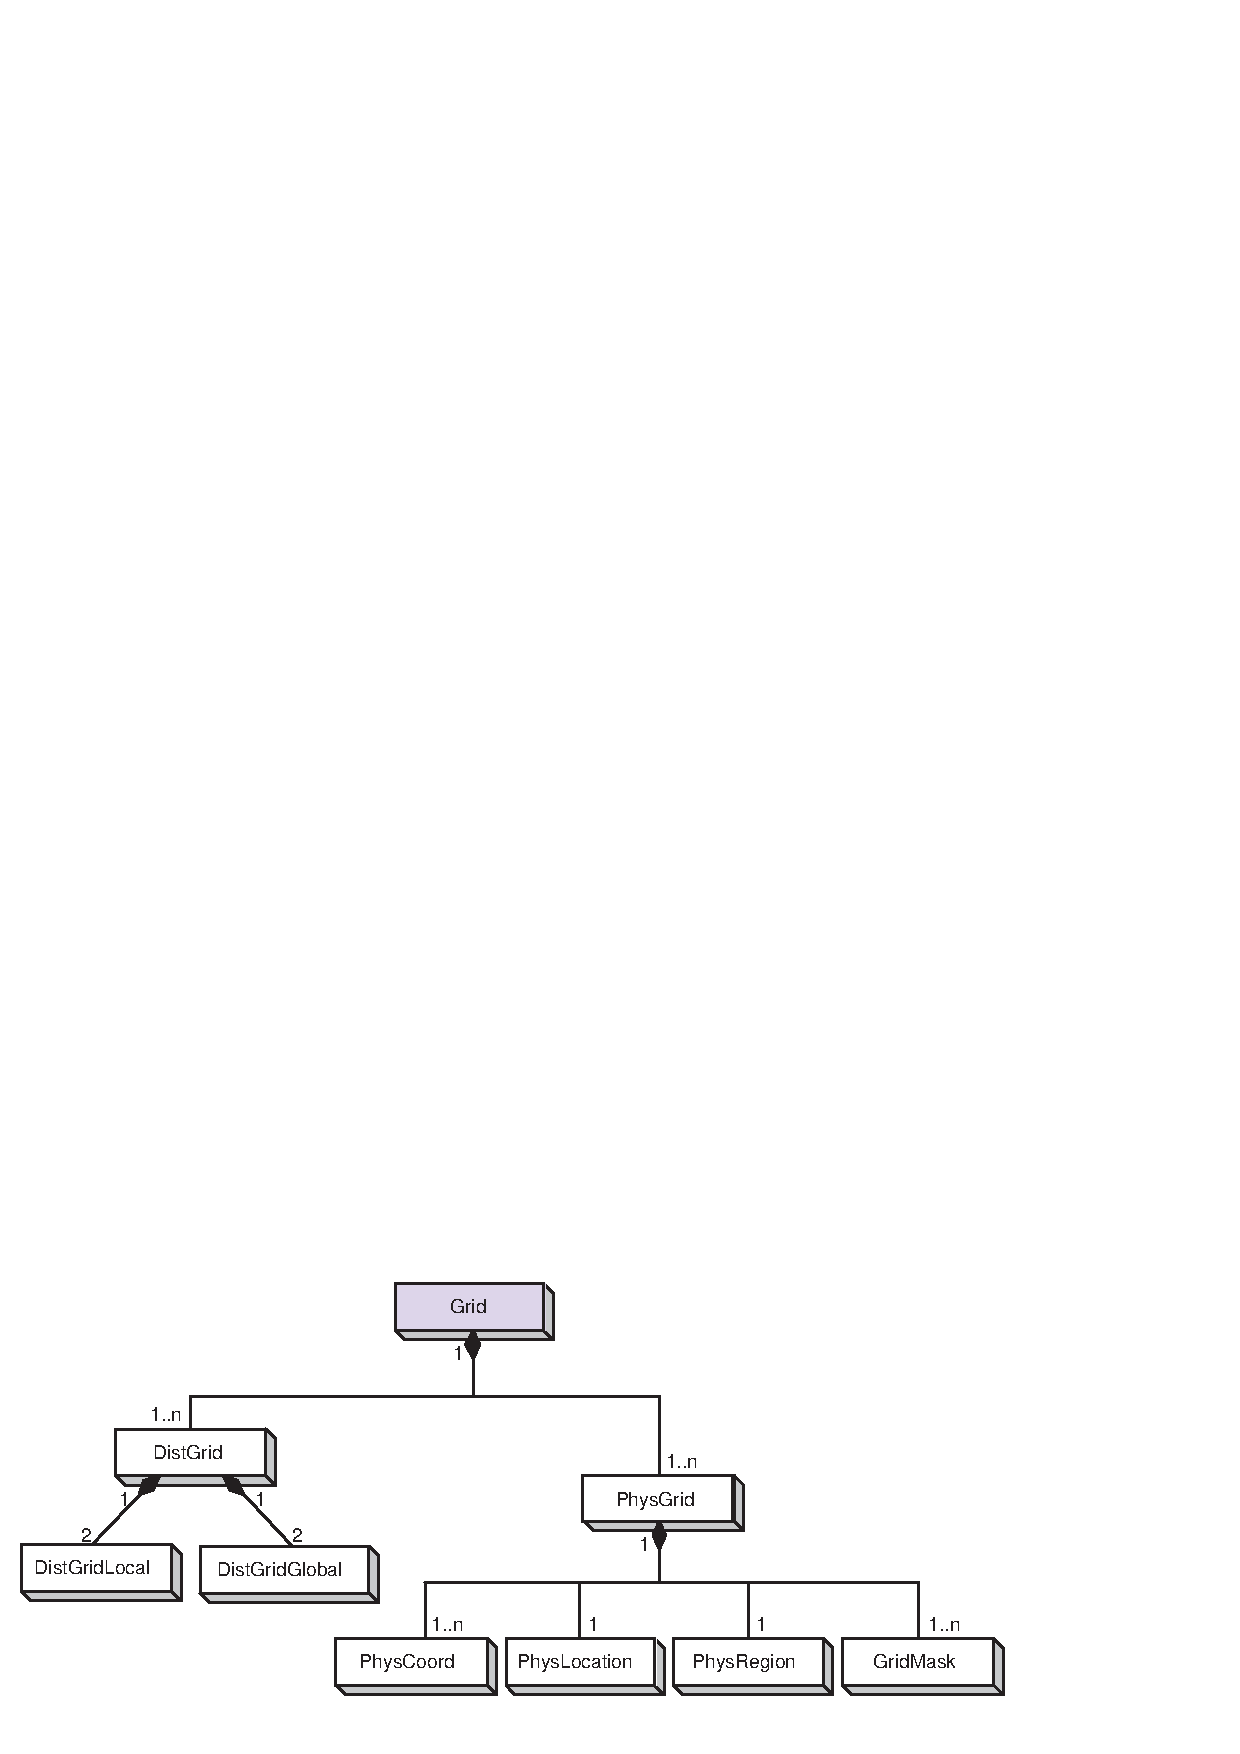
\includegraphics{Grid_obj}   
\end{center}

Each Grid contains at least one Distributed Grid and a related Physical Grid.
The Physical Grid maintains information about the global coordinates.  In
general the coordinates are described implicitly by specifying the grid type
and the corresponding parameters.  However it is possible that the Physical
Grid must be completely enumerated, perhaps in the case of assimilated data
or unstructured data.  The Distributed Grid defines an index space that
corresponds to cells in the Physical Grid and is decomposed among DEs in a
DELayout.  Please see Sections~\ref{sec:DistGridClasses} and
~\ref{sec:PhysGridClasses} for more information about the private
DistGrid and PhysGrid classes.



%#elif defined(1)
%% $Id$
%
% Earth System Modeling Framework
% Copyright 2002-2020, University Corporation for Atmospheric Research,
% Massachusetts Institute of Technology, Geophysical Fluid Dynamics
% Laboratory, University of Michigan, National Centers for Environmental
% Prediction, Los Alamos National Laboratory, Argonne National Laboratory,
% NASA Goddard Space Flight Center.
% Licensed under the University of Illinois-NCSA License.

\subsection{Object Model}

The following is a simplified UML diagram showing the structure of the
Grid class.  See Appendix A, {\it A Brief Introduction to UML},
for a translation table that lists the symbols in the diagram and their 
meaning.

\begin{center}
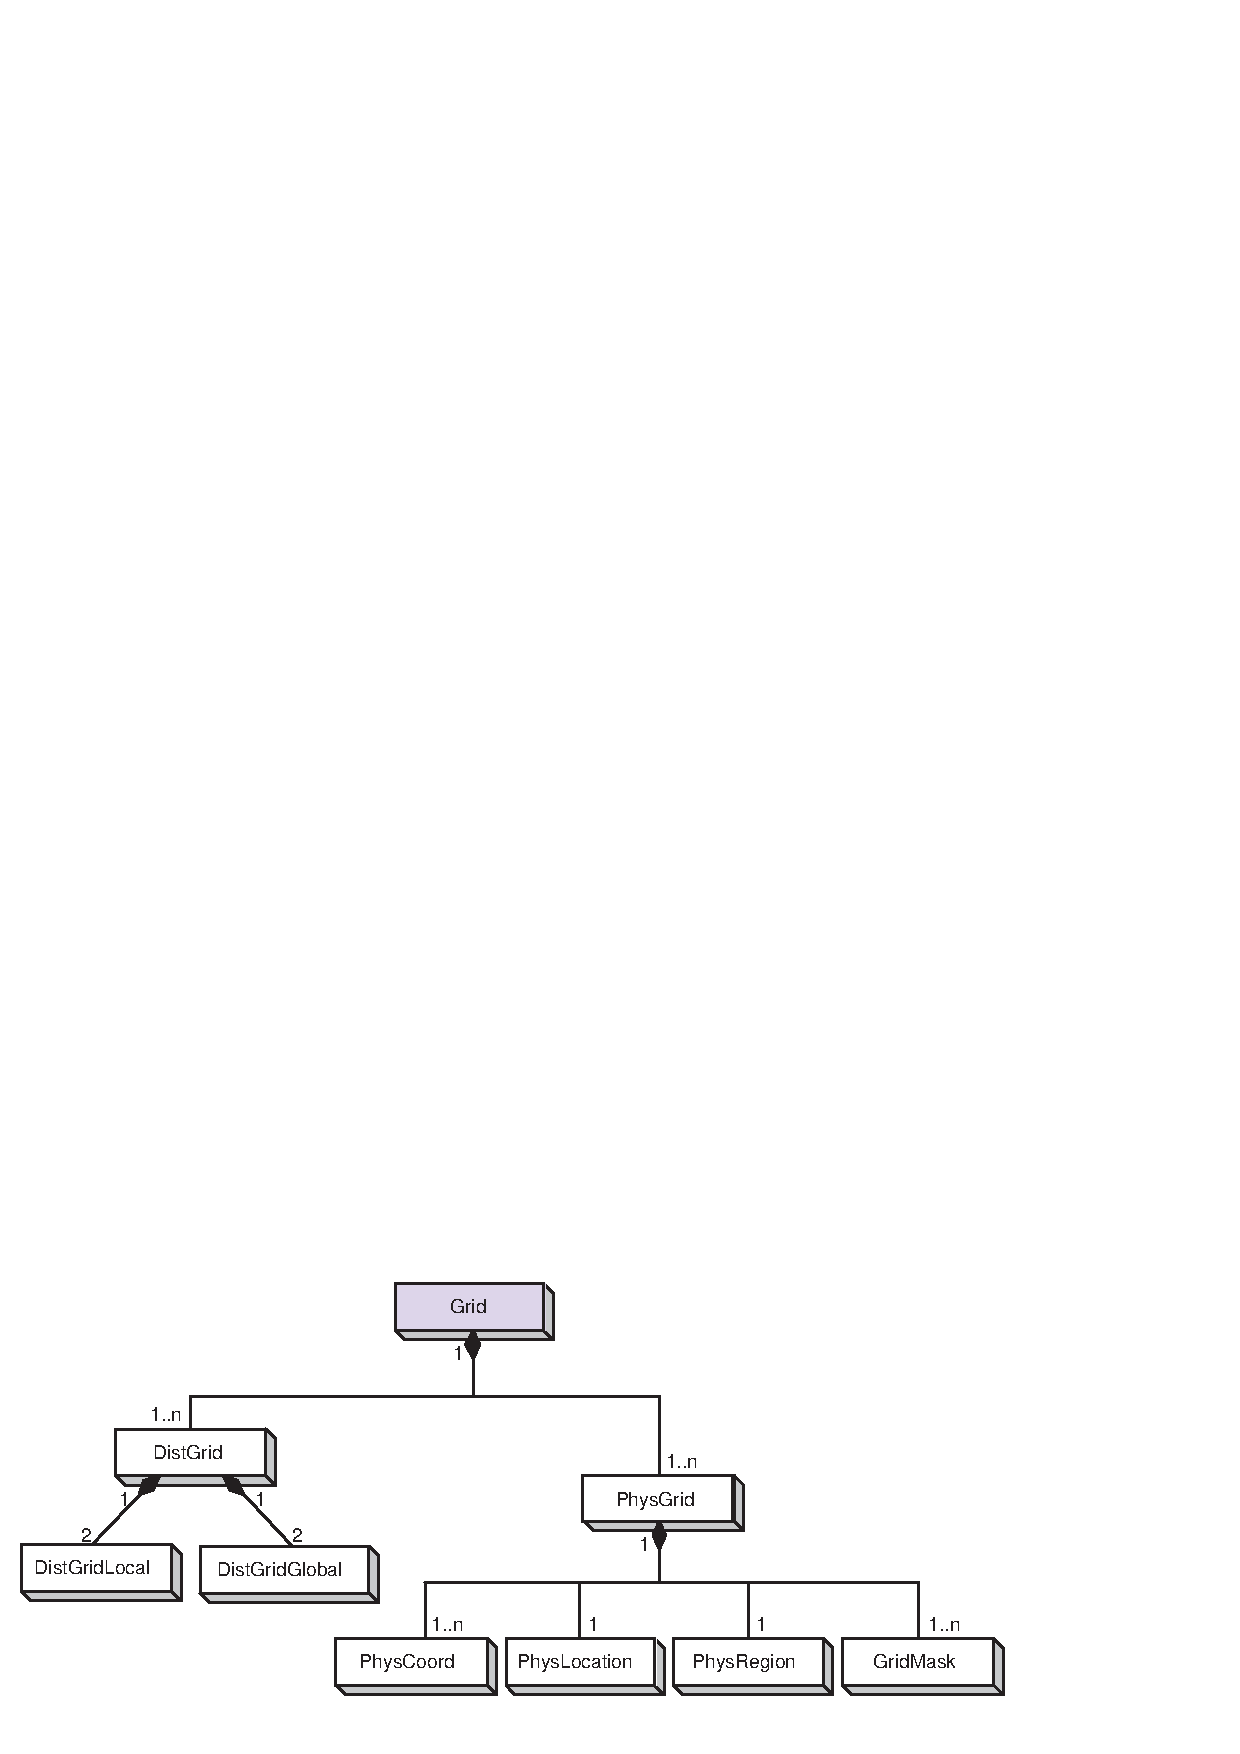
\includegraphics{Grid_obj}   
\end{center}

Each Grid contains at least one Distributed Grid and a related Physical Grid.
The Physical Grid maintains information about the global coordinates.  In
general the coordinates are described implicitly by specifying the grid type
and the corresponding parameters.  However it is possible that the Physical
Grid must be completely enumerated, perhaps in the case of assimilated data
or unstructured data.  The Distributed Grid defines an index space that
corresponds to cells in the Physical Grid and is decomposed among DEs in a
DELayout.  Please see Sections~\ref{sec:DistGridClasses} and
~\ref{sec:PhysGridClasses} for more information about the private
DistGrid and PhysGrid classes.



%#endif
\section{Grid Class}
\subsection{Description}
% $Id$
%
% Earth System Modeling Framework
% Copyright 2002-2020, University Corporation for Atmospheric Research, 
% Massachusetts Institute of Technology, Geophysical Fluid Dynamics 
% Laboratory, University of Michigan, National Centers for Environmental 
% Prediction, Los Alamos National Laboratory, Argonne National Laboratory, 
% NASA Goddard Space Flight Center.
% Licensed under the University of Illinois-NCSA License.

The ESMF Grid class is used to describe the geometry and discretization
of logically rectangular physical grids.  It also contains the
description of the grid's underlying topology and the decomposition
of the physical grid across the available computational resources.
The most frequent use of the Grid class is to describe physical grids
in user code so that sufficient information is available to perform ESMF
methods such as regridding.  

%In the current release (v5.2.0)
%the functionality in this class is partially implemented.  
%Multi-tile grids are not supported, and edge connectivities 
%are not implemented and default to aperiodic.  
%Other constraints of the current
%implementation are noted in the usage section and in the API
%descriptions.


\begin{center}
\begin{tabular}{|p{6in}|}
\hline
\vspace{.01in}
{\bf Key Features} \\[.01in]
Representation of grids formed by logically rectangular regions,
including uniform and rectilinear grids (e.g. lat-lon grids),
curvilinear grids (e.g. displaced pole grids), and grids formed
by connected logically rectangular regions (e.g. cubed sphere grids).\\
Support for 1D, 2D, 3D, and higher dimension grids.\\ 
Distribution of grids across computational resources for parallel
operations - users set which grid dimensions are distributed.\\
Grids can be created already distributed, so that no single
resource needs global information during the creation process.\\
Options to define periodicity and other edge connectivities either 
explicitly or implicitly via shape shortcuts.\\ 
Options for users to define grid coordinates themselves or call
prefabricated coordinate generation routines for standard grids
[NO GENERATION ROUTINES YET].\\
Options for incremental construction of grids.\\
Options for using a set of pre-defined stagger locations or for setting
custom stagger locations.\\ [.03in] \hline
\end{tabular}
\end{center}

\subsubsection{Grid Representation in ESMF}

ESMF Grids are based on the concepts described in {\it A Standard
Description of Grids Used in Earth System Models} [Balaji 2006].  In this document
Balaji introduces the mosaic concept as a means of describing
a wide variety of Earth system model grids.  A {\bf mosaic} is
composed of grid tiles connected at their edges.  Mosaic grids
includes simple, single tile grids as a special case.  

The ESMF Grid class is a representation of a mosaic grid.  Each ESMF
Grid is constructed of one or more logically rectangular {\bf Tiles}.
A Tile will usually have some physical significance (e.g. the region
of the world covered by one face of a cubed sphere grid).

The piece of a Tile that resides on one DE (for simple cases, a DE
can be thought of as a processor - see section on the DELayout)
is called a {\bf LocalTile}.  For example, the six faces of a cubed
sphere grid are each Tiles, and each Tile can be divided into many
LocalTiles.  

Every ESMF Grid contains a DistGrid object, which defines the Grid's
index space, topology, distribution, and connectivities.  It enables
the user to define the complex edge relationships of tripole and other
grids.  The DistGrid can be created explicitly and passed into a Grid
creation routine, or it can be created implicitly if the user takes
a Grid creation shortcut. The DistGrid used
in Grid creation describes the properties of the Grid cells. In addition
to this one, the Grid internally creates DistGrids for each stagger location. 
These stagger DistGrids are related to the original DistGrid, but may 
contain extra padding to represent the extent of the index space of
the stagger. These DistGrids are what are used when a Field is created 
on a Grid. 

\subsubsection{Supported Grids}

The range of supported grids in ESMF can be defined by:
\begin{itemize}
\item Types of topologies and shapes supported.  ESMF supports one or
more logically rectangular grid Tiles with connectivities specified
between cells.  For more details see section \ref{sec:ShapeShortcut}.
\item Types of distributions supported.  ESMF supports  regular,
irregular, or arbitrary distributions of data.  
For more details see section \ref{sec:desc:dist}.
\item Types of coordinates supported.  ESMF supports uniform, rectilinear,
and curvilinear coordinates.  For more details see section \ref{sec:coordspec}.
\end{itemize}

\subsubsection{Grid Topologies and Periodicity}
\label{sec:ShapeShortcut}
\begin{sloppypar}
ESMF has shortcuts for the creation of standard Grid topologies 
or {\bf shapes} up to 3D.  In many cases, these enable the user to
bypass the step of creating a DistGrid before creating the Grid. 
There are two sets of methods which allow the user to do this. These two sets of methods cover the same set of topologies, but
allow the user to specify them in different ways.

 The first set of these are a group of overloaded
calls broken up by the number of periodic dimensions they specify. With these the user can pick 
the method which creates a Grid with the number of periodic dimensions they need, and then specify other connectivity 
options via arguments to the method. The following is a description of these methods:  
\end{sloppypar}

\medskip

\begin{description}
\item [ESMF\_GridCreateNoPeriDim()] Allows the user to create a Grid with no edge connections, for example, a regional Grid with closed boundaries.

\item [ESMF\_GridCreate1PeriDim()] Allows the user to create a Grid with 1 periodic dimension and supports a range of options for what to do at the pole (see ~Section~\ref{const:cpolekind}. Some examples of Grids which can be created here are tripole spheres, bipole spheres, cylinders with open poles. 

\item [ESMF\_GridCreate2PeriDim()] Allows the user to create a Grid with 2 periodic dimensions, for example a torus, or a regional Grid with
doubly periodic boundaries. 
\end{description}

More detailed information can be found in the API description of each.

\medskip

\begin{sloppypar}
The second set of shortcut methods is a set of methods overloaded under the name {\tt ESMF\_GridCreate()}. These methods
allow the user to specify the connectivites at the end of each dimension, by using the ESMF\_GridConn\_Flag flag. The table below shows the ESMF\_GridConn\_Flag settings used to create 
standard shapes in 2D using the ESMF\_GridCreate() call.  Two values
are specified for each dimension, one for the low end and one for 
the high end of the dimension's index values. 
\end{sloppypar}

\medskip
\begin{tabular}{|l|c|c||c|c||}
\hline
2D Shape & {\bf connflagDim1(1)} & {\bf connflagDim1(2)}  & {\bf connflagDim2(1)} & {\bf connflagDim2(2)}  \\
\hline
{\bf Rectangle}  & NONE & NONE & NONE & NONE \\
{\bf Bipole Sphere} & POLE & POLE & PERIODIC & PERIODIC \\
{\bf Tripole Sphere} & POLE & BIPOLE & PERIODIC & PERIODIC \\
{\bf Cylinder} & NONE & NONE & PERIODIC & PERIODIC \\
{\bf Torus}  & PERIODIC & PERIODIC & PERIODIC & PERIODIC \\
\hline
\hline
\end{tabular}
\medskip

If the user's grid shape is too complex for an ESMF shortcut routine,
or involves more than three dimensions, a DistGrid can be created
to specify the shape in detail.  This DistGrid is then passed
into a Grid create call.

\subsubsection{Grid Distribution}
\label{sec:desc:dist}

ESMF Grids have several options for data distribution (also referred to
as decomposition).  As ESMF Grids are cell based, these 
options are all specified  in terms of how the cells in the Grid
are broken up between DEs. 

The main distribution options are regular, irregular, and arbitrary.
A {\bf regular} distribution is one in which the same number of
contiguous grid cells are assigned to each DE in the
distributed dimension.  An {\bf irregular} distribution is one in which
unequal numbers of contiguous grid cells are assigned to each
DE in the distributed dimension.  An {\bf arbitrary} distribution is
one in which any grid cell can be assigned to any DE.  Any of these
distribution options can be applied to any of the grid shapes (i.e.,
rectangle) or types (i.e., rectilinear).  Support for arbitrary distribution 
is limited in the current version of ESMF.


Figure \ref{fig:GridDecomps} illustrates options for distribution.
\begin{figure}
\scalebox{0.9}{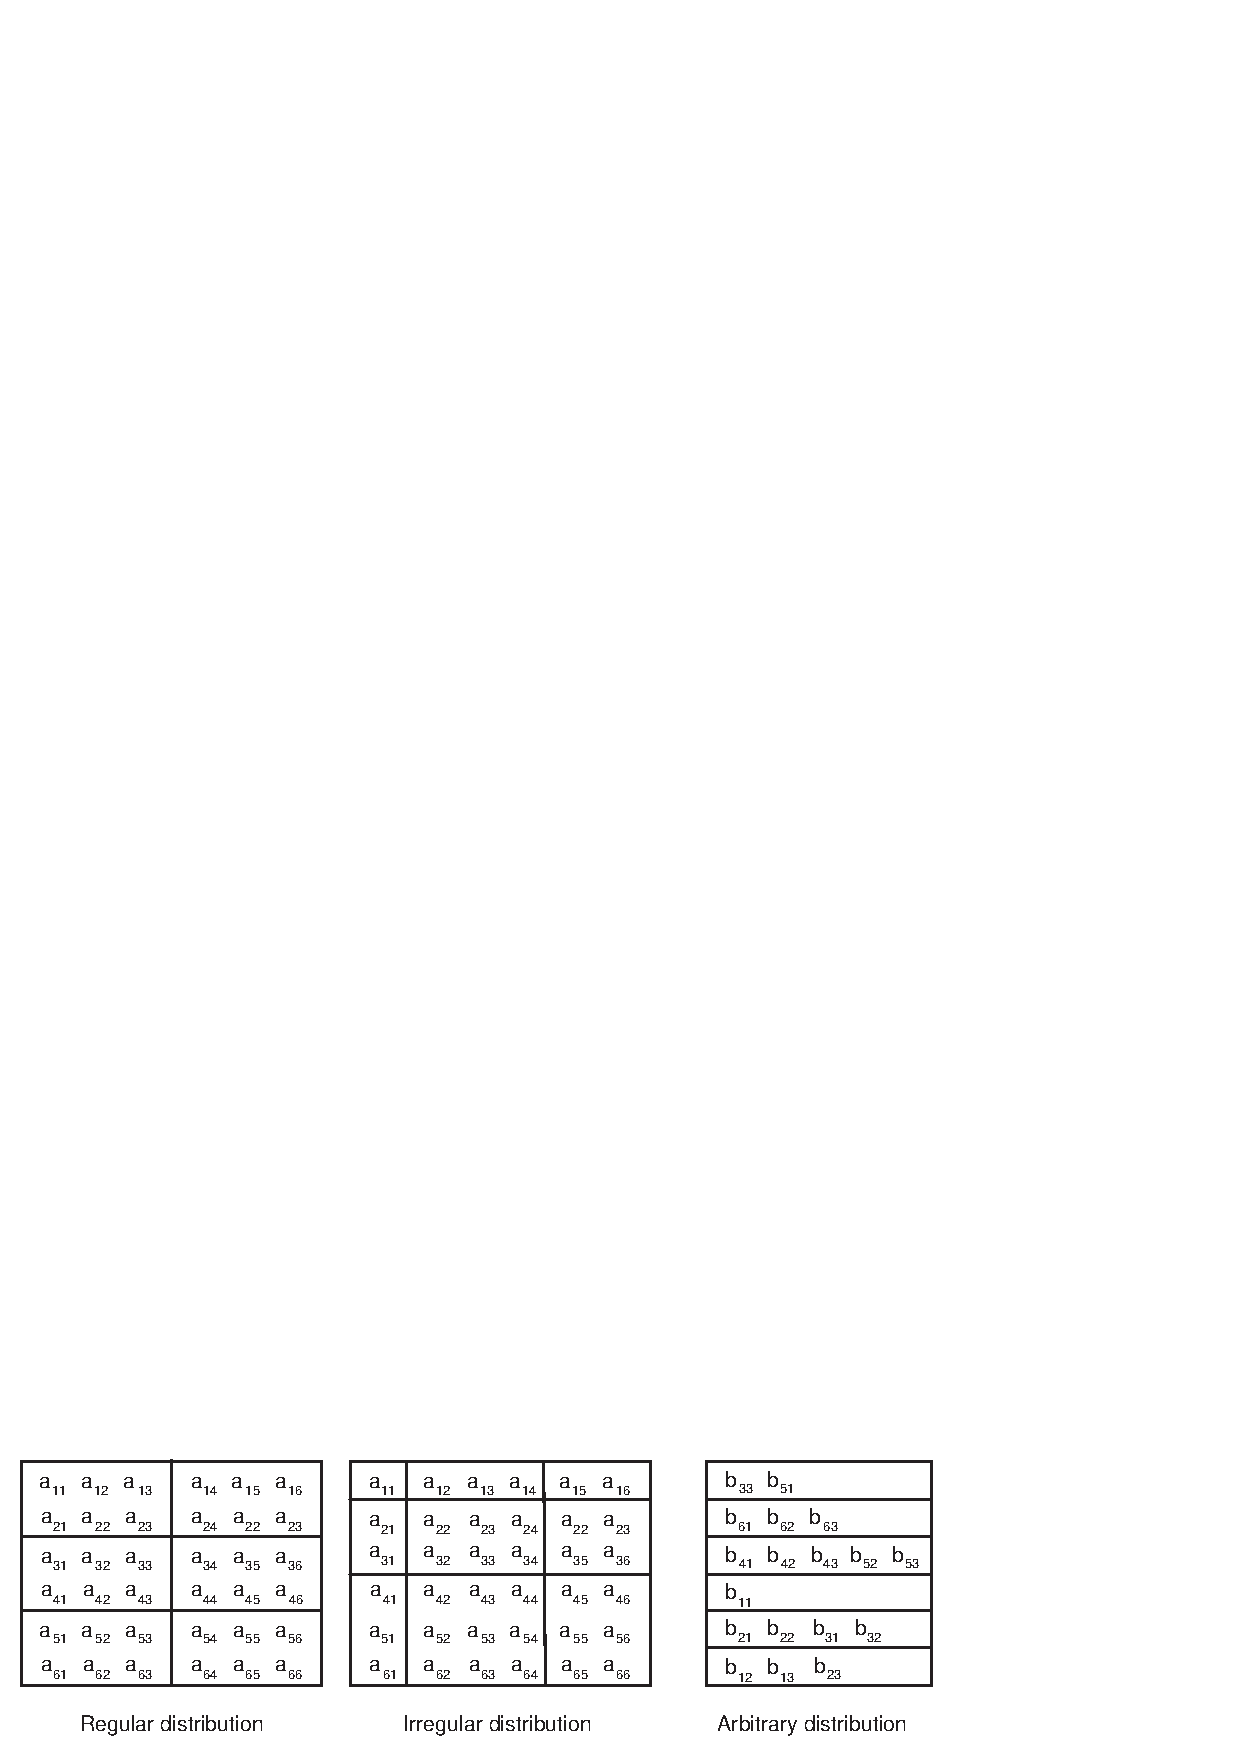
\includegraphics{GridDecomps}}
\caption{Examples of regular and irregular decomposition of
a grid {\bf a} that is 6x6, and an arbitrary decomposition of
a grid {\bf b} that is 6x3.}
\label{fig:GridDecomps}
\end{figure}

A distribution can also be specified using the DistGrid, by passing
object into a Grid create call.

\subsubsection{Grid Coordinates}
\label{sec:coordspec}
Grid Tiles can have uniform, rectilinear, or curvilinear
coordinates.  The coordinates of {\bf uniform} grids are equally spaced along
their axes, and can be fully specified by the coordinates of the two opposing points
that define the grid's physical span.  The coordinates of {\bf rectilinear} grids
are unequally spaced along their axes, and can be fully specified by giving
the spacing of grid points along each axis.  The coordinates of {\bf curvilinear 
grids} must be specified by giving the explicit set of coordinates for each
grid point.  Curvilinear grids are often uniform or rectilinear grids that 
have been warped; for example, to place a pole over a land mass so that it
does not affect the computations performed on an ocean model grid.  Figure
\ref{fig:LogRectGrids} shows examples of each type of grid.

%Any of these logically rectangular grid types can be combined through edge
%connections to form a mosaic.  Cubed sphere and yin-yang grids are examples
%of mosaic grids.  Note that as of v5.2.0 multi-tile grids have not yet been
%implemented.
 
\begin{figure}
\scalebox{0.9}{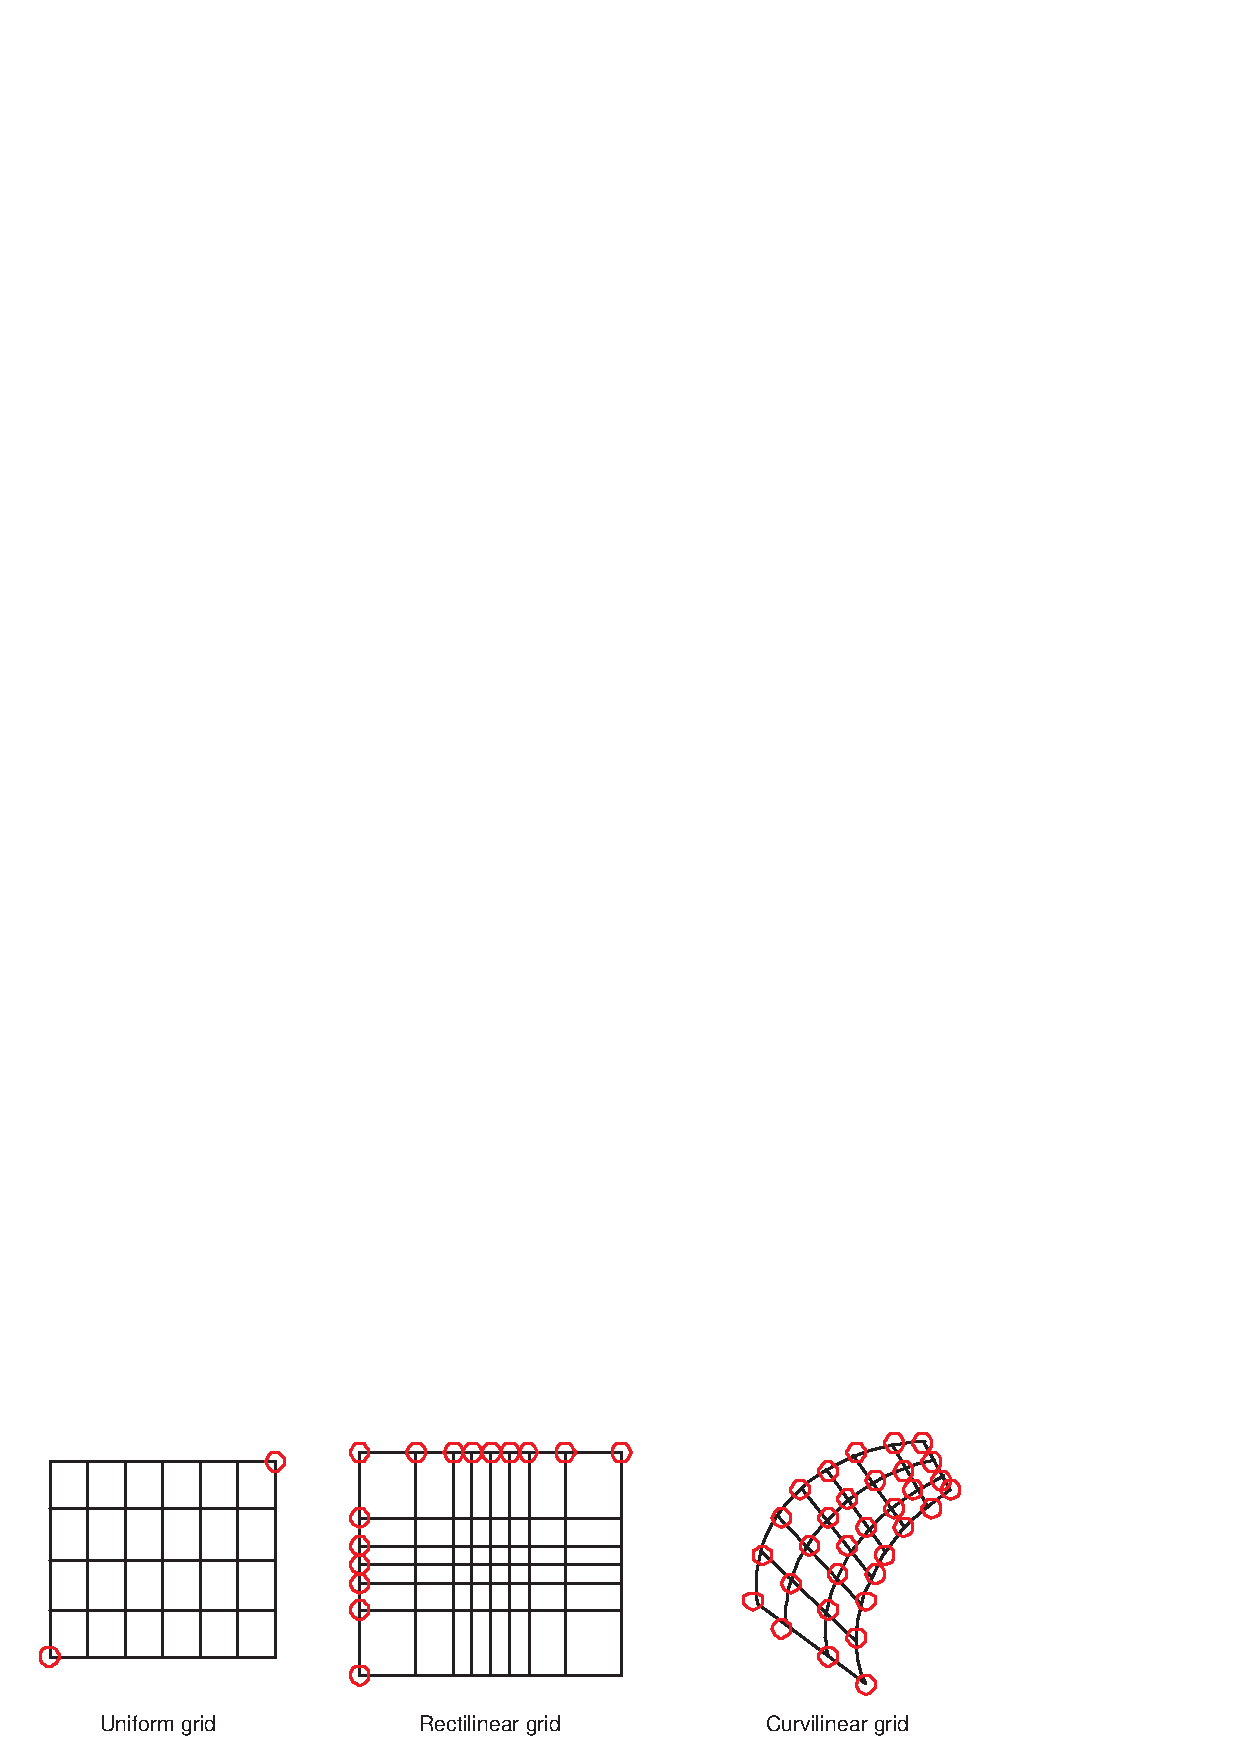
\includegraphics{LogRectGrids}}
\caption{Types of logically rectangular grid tiles.  Red circles show the
values needed to specify grid coordinates for each type.}
\label{fig:LogRectGrids}
\end{figure}

Each of these coordinate types can be set for each of the standard grid shapes
described in section \ref{sec:ShapeShortcut}.  

The table below shows how examples of common single Tile grids fall 
into this shape and coordinate taxonomy.  Note that any
of the grids in the table can have a regular or arbitrary distribution.

\medskip
\begin{tabular}{|p{.8in}|p{1.6in}|p{1.6in}|p{1.6in}|}
\hline
 & {\bf Uniform} & {\bf Rectilinear} & {\bf Curvilinear} \\ 
\hline
{\bf Sphere} & Global uniform lat-lon grid & Gaussian grid & Displaced pole grid \\
\hline
{\bf Rectangle} & Regional uniform lat-lon grid & Gaussian grid section & Polar stereographic grid section\\
\hline
\end{tabular}

\subsubsection{Coordinate Specification and Generation}

There are two ways of specifying coordinates in ESMF.  The
first way is for the user to {\bf set} the coordinates.  The second 
way is to take a shortcut and have the framework {\bf generate}
the coordinates.  

No ESMF generation routines are currently available.

%See Section~\ref{sec:usage:staggerloc} for more description and examples of
%setting coordinates.

\subsubsection{Staggering}

{\bf Staggering} is a finite difference technique in which the values 
of different physical quantities are placed at different locations
within a grid cell. 

The ESMF Grid class supports a variety of stagger locations, including
cell centers, corners, and edge centers. The default stagger location in 
ESMF is the cell center, and cell counts in Grid are based on this assumption.
Combinations of the 2D ESMF stagger locations are sufficient to specify any of the
Arakawa staggers.  ESMF also supports staggering in 3D and higher dimensions.
There are shortcuts for standard staggers, and interfaces through which users 
can create custom staggers.  

As a default the ESMF Grid class provides symmetric staggering, so
that cell centers are enclosed by cell perimeter (e.g. corner) 
stagger locations. This means the coordinate arrays for stagger
locations other than the center will have an additional element of 
padding in order to enclose the cell center locations.
However, to achieve other types of staggering, the user may alter 
or eliminate this padding by using the appropriate options when adding
coordinates to a Grid. 
 
%In v5.2.0, only the cell center stagger location is supported for an
%arbitrarily distributed grid. For examples and a full description of the stagger interface 
%see Section~\ref{sec:usage:staggerloc}. 

\subsubsection{Masking}
\label{sec:usage:items}

Masking is the process whereby parts of a grid can be marked to be
ignored during an operation, such as regridding.  Masking can be
used on a source grid to indicate that certain portions of the grid
should not be used to generate regridded data.  This is useful, for
example, if a portion of the source grid contains unusable values.
Masking can also be used on a destination grid to indicate that the
portion of the field built on that part of the Grid should not
receive regridded data.  This is useful, for example, when part of
the grid isn't being used (e.g. the land portion of an ocean grid).

ESMF regrid currently supports masking for Fields built on
structured Grids and element masking for Fields built on
unstructured Meshes. The user may mask out points in the source
Field or destination Field or both. To do masking the user sets
mask information in the Grid 
%(see \ref{sec:usage:items}) 
or Mesh 
%(see \ref{sec:mesh:mask}) 
upon which the Fields passed into the
{\tt ESMC\_FieldRegridStore()} call are built. The {\tt srcMaskValues} 
and {\tt dstMaskValues} arguments to that
call can then be used to specify which values in that mask
information indicate that a location should be masked out. For
example, if {\tt dstMaskValues} is set to (/1,2/), then any location that
has a value of 1 or 2 in the mask information of the Grid or Mesh
upon which the destination Field is built will be masked out.

Masking behavior differs slightly between regridding methods. For
non-conservative regridding methods (e.g. bilinear or high-order
patch), masking is done on points. For these methods, masking a
destination point means that that point won't participate in
regridding (e.g. won't be interpolated to). For these methods,
masking a source point means that the entire source cell using
that point is masked out. In other words, if any corner point
making up a source cell is masked then the cell is masked. For
conservative regridding methods (e.g. first-order conservative)
masking is done on cells. Masking a destination cell means that
the cell won't participate in regridding (e.g. won't be
interpolated to). Similarly, masking a source cell means that the
cell won't participate in regridding (e.g. won't be interpolated
from).  For any type of interpolation method (conservative or
non-conservative) the masking is set on the location upon
which the Fields passed into the regridding call are built.
For example, if Fields built on  {\tt ESMC\_STAGGERLOC\_CENTER} are
passed into the {\tt ESMC\_FieldRegridStore()} call then the masking
should also be set on {\tt ESMC\_STAGGERLOC\_CENTER}.

\subsection{Constants}
% $Id$

\subsubsection{ESMC\_COORDSYS}
\label{const:ccoordsys}

{\sf DESCRIPTION:\\}
 A set of values which indicates in which system the coordinates in the Grid are. This value is useful both to indicate to 
other users the type of the coordinates, but also to control how the coordinates are interpreted in regridding methods 
(e.g. {\tt ESMC\_FieldRegridStore()}).

The type of this flag is:

{\tt type(ESMC\_CoordSys\_Flag)}

The valid values are:
\begin{description}
\item [ESMC\_COORDSYS\_CART] Cartesian coordinate system. In this system, the cartesian coordinates are mapped to the Grid coordinate dimensions in the following order: x,y,z. (E.g. using {\tt coordDim=2} in ESMC\_GridGetCoord() references the y dimension) 

\item [ESMC\_COORDSYS\_SPH\_DEG] Spherical coordinates in degrees. In this system, the spherical coordinates are mapped to the Grid coordinate dimensions in the following order: longitude, latitude, radius. (E.g. using {\tt coordDim=2} in ESMC\_GridGetCoord() references the latitude dimension) Note, however, that ESMC\_FieldRegridStore() currently just supports longitude and latitude (i.e. with this system, only Grids of dimension 2 are supported in the regridding).

\item [ESMC\_COORDSYS\_SPH\_RAD] Spherical coordinates in radians. In this system, the spherical coordinates are mapped to the Grid coordinate dimensions in the following order: longitude, latitude, radius. (E.g. using {\tt coordDim=2} in ESMC\_GridGetCoord() references the latitude dimension) Note, however, that ESMC\_FieldRegridStore() currently just supports longitude and latitude (i.e. with this system, only Grids of dimension 2 are supported in the regridding).

\end{description}


\subsubsection{ESMC\_GRIDITEM}
\label{const:cgriditem}

{\sf DESCRIPTION:\\}
The ESMC Grid can contain other kinds of data besides coordinates. 
This data is referred to as Grid ``items''. Some items may be used
by ESMC for calculations involving the Grid. The following
are the valid values of ESMC\_GridItem\_Flag.

The type of this flag is:

{\tt type(ESMC\_GridItem\_Flag)}

The valid values are:
\newline
\begin{tabular}{|l|c|c|c|c||}
\hline
\hline
Item Label & {\bf Type Restriction}  & {\bf Type Default} & {\bf ESMC Uses} & {\bf Controls} \\
\hline
{\bf ESMC\_GRIDITEM\_MASK}  & ESMC\_TYPEKIND\_I4 & ESMC\_TYPEKIND\_I4 & YES & Masking in Regrid \\
{\bf ESMC\_GRIDITEM\_AREA} & NONE & ESMC\_TYPEKIND\_R8 & YES & Conservation in Regrid \\
\hline
\hline
\end{tabular}


\subsubsection{ESMC\_GRIDSTATUS}
\label{const:cgridstatus}

{\sf DESCRIPTION:\\}
The ESMC Grid class can exist in two states. These states are
present so that the library code can detect if a Grid has been
appropriately setup for the task at hand. The following
are the valid values of ESMC\_GRIDSTATUS.

The type of this flag is:

{\tt type(ESMC\_GridStatus\_Flag)}

The valid values are:
\begin{description}
\item [ESMC\_GRIDSTATUS\_EMPTY:] Status after a Grid has been created with 
      {\tt ESMC\_GridEmptyCreate}.  A Grid object container is allocated but
      space for internal objects is not.  Topology information and coordinate
      information is incomplete.  This object can be used in {\tt ESMC\_GridEmptyComplete()}
      methods in which additional information is added to the Grid.
\item [ESMC\_GRIDSTATUS\_COMPLETE:] The Grid has a specific topology and
      distribution, but incomplete coordinate arrays.  The Grid can be used
      as the basis for allocating a Field, and coordinates can be added
      via {\tt ESMC\_GridCoordAdd()} to allow other functionality. 
\end{description}


\subsubsection{ESMC\_POLEKIND}
\label{const:cpolekind}

{\sf DESCRIPTION:\\}
This type describes the type of connection that occurs at the pole when a Grid is 
created with {\tt ESMC\_GridCreate1PeriodicDim()}.

The type of this flag is:

{\tt type(ESMC\_PoleKind\_Flag)}

The valid values are:
\begin{description}
\item [ESMC\_POLEKIND\_NONE] No connection at pole.

\item [ESMC\_POLEKIND\_MONOPOLE] This edge is connected to itself. Given
that the edge is n elements long, then element i is connected to
element i+n/2.

\item [ESMC\_POLEKIND\_BIPOLE] This edge is connected to itself. Given
that the edge is n elements long, element i is connected to element n-i-1.
\end{description}


\subsubsection{ESMC\_STAGGERLOC}
\label{const:cstaggerloc}

 {\sf DESCRIPTION:\\}
 In the ESMC Grid class, data can be located at different positions in a
 Grid cell.  When setting or retrieving coordinate data the stagger location is
 specified to tell the Grid method  from where in the cell to get the data. 
 Although the user may define their own custom stagger locations, 
 ESMC provides a set of predefined locations for ease of use. The
following are the valid predefined stagger locations. 

\medskip

\begin{center}
\begin{figure}
\center
\scalebox{0.75}{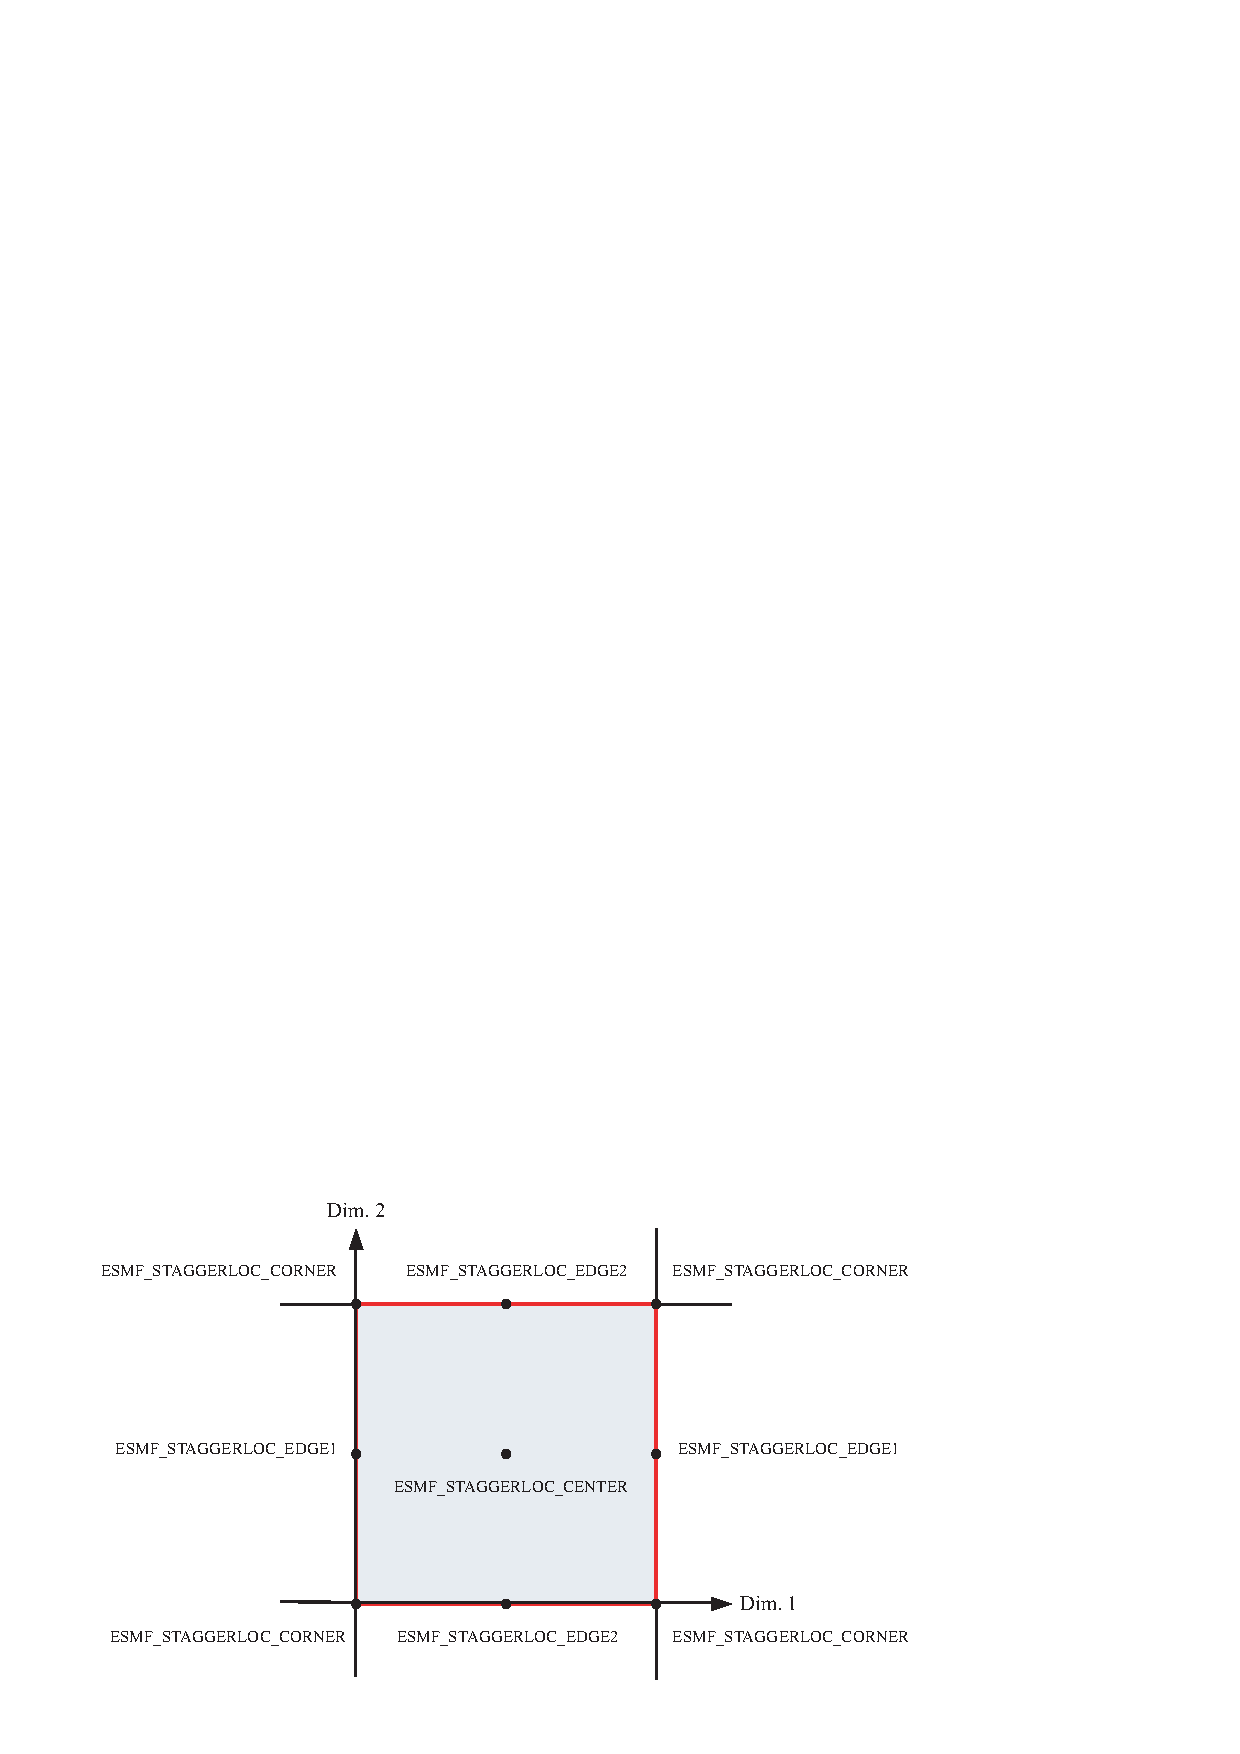
\includegraphics{GridStaggerLoc2D}}
\caption{2D Predefined Stagger Locations}
\label{fig:gridstaggerloc2d}
\end{figure}
\end{center}

The 2D predefined stagger locations (illustrated in figure~\ref{fig:gridstaggerloc2d}) are:\\
\begin{description}
\item [ESMC\_STAGGERLOC\_CENTER:] The center of the cell.
\item [ESMC\_STAGGERLOC\_CORNER:] The corners of the cell.
\item [ESMC\_STAGGERLOC\_EDGE1:] The edges offset from the center in the 1st dimension.
\item [ESMC\_STAGGERLOC\_EDGE2:] The edges offset from the center in the 2nd dimension.
\end{description}

\medskip

\begin{center}
\begin{figure}
\center
\scalebox{1.0}{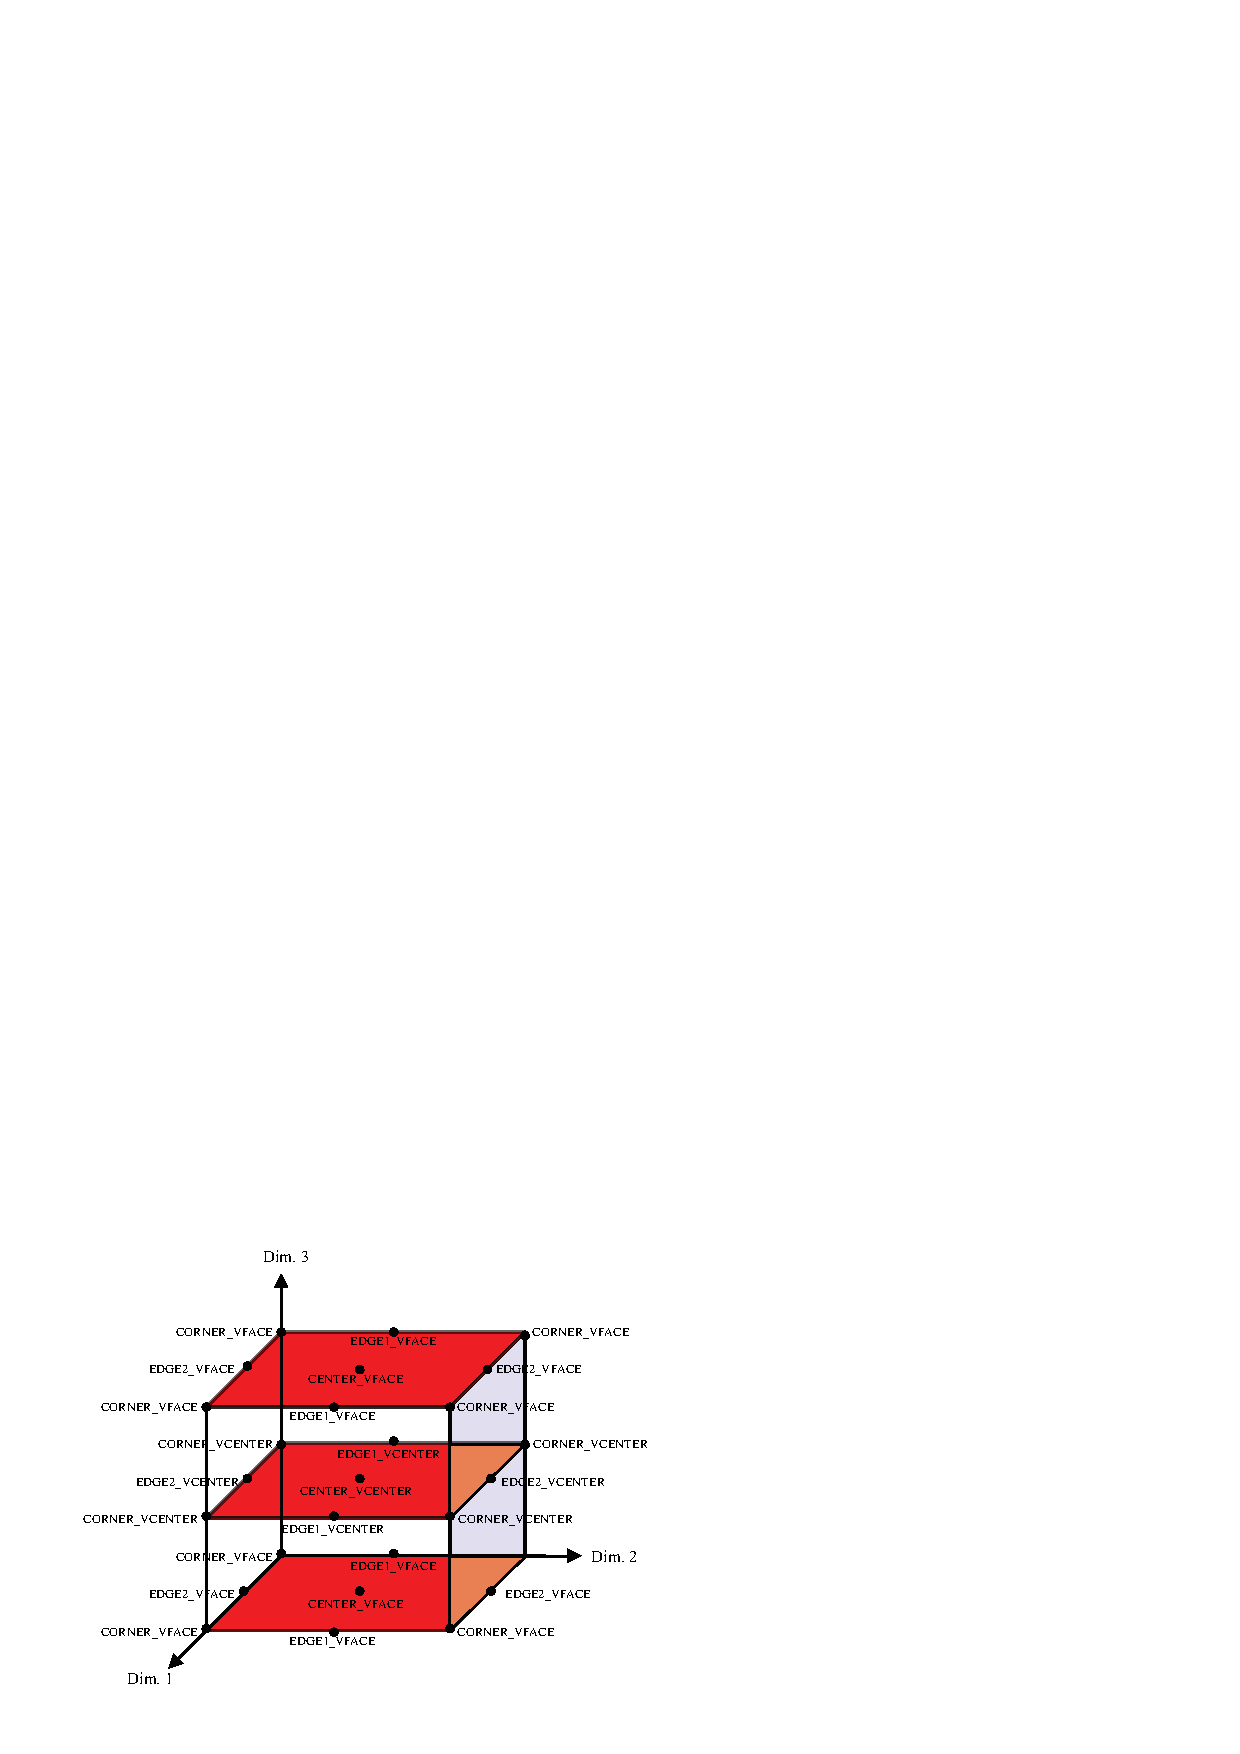
\includegraphics{GridStaggerLoc3D}}
\caption{3D Predefined Stagger Locations}
\label{fig:gridstaggerloc3d}
\end{figure}
\end{center}

The 3D predefined stagger locations (illustrated in figure~\ref{fig:gridstaggerloc3d}) are:\\
\begin{description}
\item [ESMC\_STAGGERLOC\_CENTER\_VCENTER:] The center of the 3D cell.
\item [ESMC\_STAGGERLOC\_CORNER\_VCENTER:] Half way up the vertical edges of the cell.
\item [ESMC\_STAGGERLOC\_EDGE1\_VCENTER:] The center of the face bounded by edge 1 and the vertical dimension.
\item [ESMC\_STAGGERLOC\_EDGE2\_VCENTER:] The center of the face bounded by edge 2 and the vertical dimension. 
\item [ESMC\_STAGGERLOC\_CORNER\_VFACE:] The corners of the 3D cell.
\item [ESMC\_STAGGERLOC\_EDGE1\_VFACE:] The center of the edges of the 3D cell parallel offset from the center in the 1st dimension.
\item [ESMC\_STAGGERLOC\_EDGE2\_VFACE:] The center of the edges of the 3D cell parallel offset from the center in the 2nd dimension.
\item [ESMC\_STAGGERLOC\_CENTER\_VFACE:] The center of the top and bottom face. The face bounded by the 1st and 2nd dimensions. 
\end{description}

\subsubsection{ESMC\_FILEFORMAT}
\label{const:cfileformat}

{\sf DESCRIPTION:\\}
This option is used by {\tt ESMC\_GridCreateFromFile} to specify the type of the input grid file.

The type of this flag is:

{\tt type(ESMC\_FileFormat\_Flag)}

The valid values are:
\begin{description}
\item [ESMC\_FILEFORMAT\_SCRIP] SCRIP format grid file. The SCRIP format is the format accepted by the SCRIP regridding tool~\cite{ref:SCRIP}.   For Grid creation, files of this type only work when the {\tt grid\_rank} in the file is equal to 2.

\item [ESMC\_FILEFORMAT\_GRIDSPEC] a single tile grid file comforming with the proposed CF-GRIDSPEC conventions.
\end{description}

%\subsection{Use and Examples}
%% $Id$

This section describes the use of the ESMF Grid class. It first discusses
the more user friendly shape specific interface to the Grid. 
During this discussion it covers creation and options, 
adding stagger locations, coordinate data access, and other grid 
functionality. After this initial phase the document discusses 
the more advanced options which the user can employ should they
need more customized interaction with the Grid class.




 









%%                **** IMPORTANT NOTICE *****
% This LaTeX file has been automatically produced by ProTeX v. 1.1
% Any changes made to this file will likely be lost next time
% this file is regenerated from its source. Send questions 
% to Arlindo da Silva, dasilva@gsfc.nasa.gov
 
\setlength{\oldparskip}{\parskip}
\setlength{\parskip}{1.5ex}
\setlength{\oldparindent}{\parindent}
\setlength{\parindent}{0pt}
\setlength{\oldbaselineskip}{\baselineskip}
\setlength{\baselineskip}{11pt}
 
%--------------------- SHORT-HAND MACROS ----------------------
\def\bv{\begin{verbatim}}
\def\ev{\end{verbatim}}
\def\be{\begin{equation}}
\def\ee{\end{equation}}
\def\bea{\begin{eqnarray}}
\def\eea{\end{eqnarray}}
\def\bi{\begin{itemize}}
\def\ei{\end{itemize}}
\def\bn{\begin{enumerate}}
\def\en{\end{enumerate}}
\def\bd{\begin{description}}
\def\ed{\end{description}}
\def\({\left (}
\def\){\right )}
\def\[{\left [}
\def\]{\right ]}
\def\<{\left  \langle}
\def\>{\right \rangle}
\def\cI{{\cal I}}
\def\diag{\mathop{\rm diag}}
\def\tr{\mathop{\rm tr}}
%-------------------------------------------------------------

\markboth{Left}{Source File: ESMF\_GridUsageEx.F90,  Date: Tue May  5 20:59:48 MDT 2020
}

 
%/////////////////////////////////////////////////////////////

  
  \subsubsection{Create single-tile Grid shortcut method}
 
   The set of methods {\tt ESMF\_GridCreateNoPeriDim()}, {\tt ESMF\_GridCreate1PeriDim()},
   {\tt ESMF\_GridCreate2PeriDim()}, and {\tt ESMF\_GridCreate()} are shortcuts
   for building 2D or 3D single tile logically rectangular Grids.
   These methods support all three types of distributions described in
   Section~\ref{sec:desc:dist}: regular, irregular and arbitrary.
  
   The ESMF Grid is cell based and so for all distribution
   options the methods take as input the number of cells to describe
   the total index space and the number of cells to specify distribution.
  
   To create a Grid
   with a regular distribution the user specifies the global
   maximum and minimum ranges of the Grid cell index space ({\tt maxIndex} and
   {\tt minIndex}), and the number of pieces in which to partition
   each dimension (via a {\tt regDecomp} argument).
   ESMF then divides the index space as evenly as possible
   into the specified number of pieces. If there are cells
   left over then they are distributed one per DE starting from
   the first DE until they are gone.
  
   If {\tt minIndex} is
   not specified, then the bottom of the Grid cell index range is assumed
   to be (1,1,...,1). If {\tt regDecomp} is not specified, then
   by default ESMF creates a distribution that partitions the
   grid cells in the first dimension (e.g. NPx1x1...1) as evenly
   as possible by  the number of PETs NP.
   The remaining dimensions are not partitioned.
   The dimension of the Grid is the size of {\tt maxIndex}.
   The following is an example of creating a 10x20x30 3D grid
   where the first dimensions is broken into 2 pieces, the second
   is broken into 4 pieces, and the third is not divided (i.e. every DE will
   have length 30 in the 3rd dimension). 
%/////////////////////////////////////////////////////////////

 \begin{verbatim}
  grid3D=ESMF_GridCreateNoPeriDim(regDecomp=(/2,4,1/), maxIndex=(/10,20,30/), &
           rc=rc)
 
\end{verbatim}
 
%/////////////////////////////////////////////////////////////

   Irregular distribution requires the user to specify the
   exact number of Grid cells per DE in each dimension.  In the
   {\tt ESMF\_GridCreateNoPeriDim()} call the {\tt countsPerDEDim1},
   {\tt countsPerDim2}, and {\tt countsPerDim3}
   arguments are used to specify a rectangular distribution
   containing size(countsPerDEDim1) by size(countsPerDEDim2) by
   size(countsPerDEDim3) DEs. The entries in each of these arrays
   specify the number of grid cells per DE in that dimension.
   The dimension of the grid is determined by the presence of
   {\tt countsPerDEDim3}.  If it's present the Grid
   will be 3D. If just {\tt countsPerDEDim1} and
   {\tt countsPerDEDim2} are specified the Grid
   will be 2D.
  
   The following call illustrates the creation of
   a 10x20 two dimensional rectangular Grid distributed across six DEs
   that are arranged 2x3.  In the first dimension there are 3 grid
   cells on the first DE and 7 cells on the second DE.  The second
   dimension has 3 DEs with 11,2, and 7 cells, respectively. 
%/////////////////////////////////////////////////////////////

 \begin{verbatim}
   grid2D=ESMF_GridCreateNoPeriDim(countsPerDEDim1=(/3,7/), &
          countsPerDEDim2=(/11,2,7/), rc=rc)

 
\end{verbatim}
 
%/////////////////////////////////////////////////////////////

   To add a distributed third dimension of size 30, broken up into
   two groups of 15, the above call would be altered as follows. 
%/////////////////////////////////////////////////////////////

 \begin{verbatim}
   grid3d=ESMF_GridCreateNoPeriDim(countsPerDEDim1=(/3,7/), &
          countsPerDEDim2=(/11,2,7/), countsPerDEDim3=(/15,15/), rc=rc)
 
\end{verbatim}
 
%/////////////////////////////////////////////////////////////

   To make a third dimension distributed across only 1 DE, then
   {\tt countsPerDEDim3} in the call should only have a single term. 
%/////////////////////////////////////////////////////////////

 \begin{verbatim}
   grid3D=ESMF_GridCreateNoPeriDim(countsPerDEDim1=(/3,7/),  &
          countsPerDEDim2=(/11,2,7/), countsPerDEDim3=(/30/), rc=rc)
 
\end{verbatim}
 
%/////////////////////////////////////////////////////////////

  
   \begin{sloppypar}
   The {\tt petMap} parameter may be used to specify on to which specific PETs
   the DEs in the Grid are assigned. Each entry in {\tt petMap} specifies to which PET the corresponding
   DE should be assigned. For example, {\tt petMap(3,2)=4} tells the Grid
   create call to put the DE located at column 3 row 2 on PET 4.
   Note that this parameter is only available for the
   regular and irregular distribution types. The {\tt petMap}
   array is a 3D array, for a 3D Grid each of its dimensions correspond to a
   Grid dimension. If the Grid is 2D, then the first two dimensions correspond
   to Grid dimensions and the last dimension should be of size 1.
   The size of each {\tt petMap} dimension is
   the number of DE's along that dimension in the Grid. For a
   regular Grid, the size is equal to the number in regDecomp
   (i.e. {\tt size(petMap,d)=regDecomp(d)} for all dimensions {\tt d} in the Grid). For
   an irregular Grid the size is equal to the number of items in
   the corresponding {\tt countsPerDEDim} variable (i.e.
   {\tt size(petMap,d)=size(countsPerDEDimd)} for all dimensions {\tt d} in the Grid).
   The following example demonstrates how to specify the PET to DE association
   for an {\tt ESMF\_GridCreateNoPeriDim()} call.
   \end{sloppypar}
   
%/////////////////////////////////////////////////////////////

 \begin{verbatim}
   ! allocate memory for petMap
   allocate( petMap(2,2,1) )

   ! Set petMap
   petMap(:,1,1) = (/3,2/) ! DE (1,1,1) on PET 3 and DE (2,1,1) on PET 2
   petMap(:,2,1) = (/1,0/) ! DE (1,2,1) on PET 1 and DE (2,2,1) on PET 0


   ! Let the 3D grid be be distributed only in the first two dimensions.
   grid2D=ESMF_GridCreateNoPeriDim(countsPerDEDim1=(/3,7/), &
           countsPerDEDim2=(/7,6/), petMap=petMap, rc=rc)
 
\end{verbatim}
 
%/////////////////////////////////////////////////////////////

   To create an grid with arbitrary distribution, the user specifies the global minimum and maximum
   ranges of the index space with the
   arguments {\tt minIndex} and {\tt maxIndex}, the total number of cells and their index space locations
   residing on the local PET through a {\tt localArbIndexCount} and a {\tt localArbIndex}
   argument. {\tt localArbIndex} is a 2D array with size {\tt (localArbIndexCount, n)} where n is the total number
   dimensions distributed arbitrarily.
   Again, if {\tt minIndex} is  not specified, then the bottom of the
   index range is assumed to be (1,1,...).
   The dimension of the Grid is equal to the size of {\tt maxIndex}.
   If n (number of arbitrarily distributed dimension) is less than the grid dimension, an optional
   argument {\tt distDim} is used to specify which of the grid dimension is arbitrarily distributed.
   If not given, the first n dimensions are assumed to be distributed.
  
   The following example creates a 2D Grid of dimensions 5x5, and places
   the diagonal elements (i.e. indices (i,i) where i goes from 1 to 5)
   on the local PET. The remaining PETs would individually declare
   the remainder of the Grid locations. 
%/////////////////////////////////////////////////////////////

 \begin{verbatim}
   ! allocate memory for localArbIndex
   allocate( localArbIndex(5,2) )
   ! Set local indices
   localArbIndex(1,:)=(/1,1/)
   localArbIndex(2,:)=(/2,2/)
   localArbIndex(3,:)=(/3,3/)
   localArbIndex(4,:)=(/4,4/)
   localArbIndex(5,:)=(/5,5/)

   ! Create a 2D Arbitrarily distributed Grid
   grid2D=ESMF_GridCreateNoPeriDim(maxIndex=(/5,5/), &
         arbIndexList=localArbIndex, arbIndexCount=5, rc=rc)
 
\end{verbatim}
 
%/////////////////////////////////////////////////////////////

  
   To create a 3D Grid of dimensions 5x6x5 with the first and the third dimensions distributed arbitrarily,
   {\tt distDim} is used. 
%/////////////////////////////////////////////////////////////

 \begin{verbatim}
   ! Create a 3D Grid with the 1st and 3rd dimension arbitrarily distributed
   grid3D=ESMF_GridCreateNoPeriDim(maxIndex=(/5,6,5/), &
         arbIndexList=localArbIndex, arbIndexCount=5, &
         distDim=(/1,3/), rc=rc)
 
\end{verbatim}
 
%/////////////////////////////////////////////////////////////

  \subsubsection{Create a 2D regularly distributed rectilinear Grid
                    with uniformly spaced coordinates}
   \label{example:2DRegUniGrid}
  
   The following is an example of creating a simple rectilinear grid
   and loading in a set of coordinates. It illustrates a straightforward use
   of the {\tt ESMF\_GridCreateNoPeriDim()} call described in the previous section.
   This code creates a 10x20 2D grid with uniformly spaced coordinates varying from (10,10) to (100,200).
   The grid is partitioned using a regular distribution. The first dimension
   is divided into two pieces, and the second dimension is divided into 3.
   This example assumes that the code is being run with a 1-1 mapping between
   PETs and DEs because we are only accessing the first DE on each PET (localDE=0).
   Because we have 6 DEs (2x3), this example would only work when run on 6 PETs.
   The Grid is created with global indices. After Grid creation the
   local bounds and native Fortran arrays are retrieved and the
   coordinates are set by the user.
   
%/////////////////////////////////////////////////////////////

 \begin{verbatim}
   !-------------------------------------------------------------------
   ! Create the Grid:  Allocate space for the Grid object, define the
   ! topology and distribution of the Grid, and specify that it
   ! will have global indices.  Note that here aperiodic bounds are
   ! specified by the argument name. In this call the minIndex hasn't
   ! been set, so it defaults to (1,1,...). The default is to
   ! divide the index range as equally as possible among the DEs
   ! specified in regDecomp. This behavior can be changed by
   ! specifying decompFlag.
   !-------------------------------------------------------------------
   grid2D=ESMF_GridCreateNoPeriDim(          &
         ! Define a regular distribution
         maxIndex=(/10,20/), & ! define index space
         regDecomp=(/2,3/),  & ! define how to divide among DEs
         coordSys=ESMF_COORDSYS_CART, &
         ! Specify mapping of coords dim to Grid dim
         coordDep1=(/1/), & ! 1st coord is 1D and depends on 1st Grid dim
         coordDep2=(/2/), & ! 2nd coord is 1D and depends on 2nd Grid dim
         indexflag=ESMF_INDEX_GLOBAL, &
         rc=rc)
 
\end{verbatim}
 
%/////////////////////////////////////////////////////////////

 \begin{verbatim}

   !-------------------------------------------------------------------
   ! Allocate coordinate storage and associate it with the center
   ! stagger location.  Since no coordinate values are specified in
   ! this call no coordinate values are set yet.
   !-------------------------------------------------------------------
   call ESMF_GridAddCoord(grid2D,  &
          staggerloc=ESMF_STAGGERLOC_CENTER, rc=rc)
 
\end{verbatim}
 
%/////////////////////////////////////////////////////////////

 \begin{verbatim}


   !-------------------------------------------------------------------
   ! Get the pointer to the first coordinate array and the bounds
   ! of its global indices on the local DE.
   !-------------------------------------------------------------------
   call ESMF_GridGetCoord(grid2D, coordDim=1, localDE=0, &
          staggerloc=ESMF_STAGGERLOC_CENTER, &
          computationalLBound=lbnd, computationalUBound=ubnd, &
          farrayPtr=coordX, rc=rc)
 
\end{verbatim}
 
%/////////////////////////////////////////////////////////////

 \begin{verbatim}

   !-------------------------------------------------------------------
   ! Calculate and set coordinates in the first dimension [10-100].
   !-------------------------------------------------------------------
   do i=lbnd(1),ubnd(1)
        coordX(i) = i*10.0
   enddo

   !-------------------------------------------------------------------
   ! Get the pointer to the second coordinate array and the bounds of
   ! its global indices on the local DE.
   !-------------------------------------------------------------------
   call ESMF_GridGetCoord(grid2D, coordDim=2, localDE=0, &
          staggerloc=ESMF_STAGGERLOC_CENTER, &
          computationalLBound=lbnd, computationalUBound=ubnd, &
          farrayPtr=coordY, rc=rc)
 
\end{verbatim}
 
%/////////////////////////////////////////////////////////////

 \begin{verbatim}


   !-------------------------------------------------------------------
   ! Calculate and set coordinates in the second dimension [10-200]
   !-------------------------------------------------------------------
   do j=lbnd(1),ubnd(1)
        coordY(j) = j*10.0
   enddo
 
\end{verbatim}
 
%/////////////////////////////////////////////////////////////

  \subsubsection{Create a periodic 2D regularly distributed rectilinear Grid}
   \label{example:2DPeriRegUniGrid}
  
   The following is an example of creating a simple rectilinear grid
   with a periodic dimension and loading in a set of coordinates. It illustrates a straightforward use
   of the {\tt ESMF\_GridCreate1PeriDim()} call described in the previous section.
   This code creates a 360x180 2D grid with uniformly spaced coordinates varying from (1,1) to (360,180).
   The grid is partitioned using a regular distribution. The first dimension
   is divided into two pieces, and the second dimension is divided into 3.
   This example assumes that the code is being run with a 1-1 mapping between
   PETs and DEs because we are only accessing the first DE on each PET (localDE=0).
   Because we have 6 DEs (2x3), this example would only work when run on 6 PETs.
   The Grid is created with global indices. After Grid creation the
   local bounds and native Fortran arrays are retrieved and the
   coordinates are set by the user.
   
%/////////////////////////////////////////////////////////////

 \begin{verbatim}
   !-------------------------------------------------------------------
   ! Create the Grid:  Allocate space for the Grid object, define the
   ! topology and distribution of the Grid, and specify that it
   ! will have global indices.  Note that here a single periodic connection
   ! is specified by the argument name. In this call the minIndex hasn't
   ! been set, so it defaults to (1,1,...). The default is to
   ! divide the index range as equally as possible among the DEs
   ! specified in regDecomp. This behavior can be changed by
   ! specifying decompFlag. Since the coordinate system is
   ! not specified, it defaults to ESMF_COORDSYS_SPH_DEG.
   !-------------------------------------------------------------------
   grid2D=ESMF_GridCreate1PeriDim(          &
         ! Define a regular distribution
         maxIndex=(/360,180/), & ! define index space
         regDecomp=(/2,3/),  & ! define how to divide among DEs
         ! Specify mapping of coords dim to Grid dim
         coordDep1=(/1/), & ! 1st coord is 1D and depends on 1st Grid dim
         coordDep2=(/2/), & ! 2nd coord is 1D and depends on 2nd Grid dim
         indexflag=ESMF_INDEX_GLOBAL, &
         rc=rc)
 
\end{verbatim}
 
%/////////////////////////////////////////////////////////////

 \begin{verbatim}


   !-------------------------------------------------------------------
   ! Allocate coordinate storage and associate it with the center
   ! stagger location.  Since no coordinate values are specified in
   ! this call no coordinate values are set yet.
   !-------------------------------------------------------------------
   call ESMF_GridAddCoord(grid2D,  &
          staggerloc=ESMF_STAGGERLOC_CENTER, rc=rc)

 
\end{verbatim}
 
%/////////////////////////////////////////////////////////////

 \begin{verbatim}

   !-------------------------------------------------------------------
   ! Get the pointer to the first coordinate array and the bounds
   ! of its global indices on the local DE.
   !-------------------------------------------------------------------
   call ESMF_GridGetCoord(grid2D, coordDim=1, localDE=0, &
          staggerloc=ESMF_STAGGERLOC_CENTER, &
          computationalLBound=lbnd, computationalUBound=ubnd, &
          farrayPtr=coordX, rc=rc)
 
\end{verbatim}
 
%/////////////////////////////////////////////////////////////

 \begin{verbatim}


   !-------------------------------------------------------------------
   ! Calculate and set coordinates in the first dimension [10-100].
   !-------------------------------------------------------------------
   do i=lbnd(1),ubnd(1)
        coordX(i) = i*1.0
   enddo

   !-------------------------------------------------------------------
   ! Get the pointer to the second coordinate array and the bounds of
   ! its global indices on the local DE.
   !-------------------------------------------------------------------
   call ESMF_GridGetCoord(grid2D, coordDim=2, localDE=0, &
          staggerloc=ESMF_STAGGERLOC_CENTER, &
          computationalLBound=lbnd, computationalUBound=ubnd, &
          farrayPtr=coordY, rc=rc)
 
\end{verbatim}
 
%/////////////////////////////////////////////////////////////

 \begin{verbatim}


   !-------------------------------------------------------------------
   ! Calculate and set coordinates in the second dimension [10-200]
   !-------------------------------------------------------------------
   do j=lbnd(1),ubnd(1)
        coordY(j) = j*1.0
   enddo
 
\end{verbatim}
 
%/////////////////////////////////////////////////////////////

  
   The remaining examples in this section will use the irregular
   distribution because of its greater generality. To create code similar to these, but
   using a regular distribution, replace the {\tt countsPerDEDim} arguments
   in the Grid create with the appropriate {\tt maxIndex} and {\tt regDecomp} arguments.
  
  \subsubsection{Create a 2D irregularly distributed rectilinear Grid
                    with uniformly spaced coordinates}
   \label{example:2DIrregUniGrid}
  
   This example serves as an illustration of the difference between using
   a regular and irregular distribution. It repeats the previous example
   except using an irregular distribution to give the user more control
   over how the cells are divided between the DEs. As before, this code
   creates a 10x20 2D Grid with uniformly spaced coordinates  varying from (10,10) to (100,200).
   In this example, the Grid is partitioned using an irregular distribution. The first dimension
   is divided into two pieces, the first with 3 Grid cells per
   DE and the second with 7 Grid cells per DE. In the second dimension,
   the Grid is divided into 3 pieces, with 11, 2, and 7 cells per DE respectively.
   This example assumes that the code is being run with a 1-1 mapping between
   PETs and DEs because we are only accessing the first DE on each PET (localDE=0).
   Because we have 6 DEs (2x3), this example would only work when run on 6 PETs.
   The Grid is created with global indices. After Grid creation the
   local bounds and native Fortran arrays are retrieved and the
   coordinates are set by the user.
   
%/////////////////////////////////////////////////////////////

 \begin{verbatim}
   !-------------------------------------------------------------------
   ! Create the Grid:  Allocate space for the Grid object, define the
   ! topology and distribution of the Grid, and specify that it
   ! will have global coordinates.  Note that aperiodic bounds are
   ! indicated by the method name. In this call the minIndex hasn't
   ! been set, so it defaults to (1,1,...).
   !-------------------------------------------------------------------
   grid2D=ESMF_GridCreateNoPeriDim(          &
            ! Define an irregular distribution
            countsPerDEDim1=(/3,7/),    &
            countsPerDEDim2=(/11,2,7/), &
            ! Specify mapping of coords dim to Grid dim
            coordDep1=(/1/), & ! 1st coord is 1D and depends on 1st Grid dim
            coordDep2=(/2/), & ! 2nd coord is 1D and depends on 2nd Grid dim
            indexflag=ESMF_INDEX_GLOBAL, &
            rc=rc)
 
\end{verbatim}
 
%/////////////////////////////////////////////////////////////

 \begin{verbatim}


   !-------------------------------------------------------------------
   ! Allocate coordinate storage and associate it with the center
   ! stagger location.  Since no coordinate values are specified in
   ! this call no coordinate values are set yet.
   !-------------------------------------------------------------------
   call ESMF_GridAddCoord(grid2D,  &
          staggerloc=ESMF_STAGGERLOC_CENTER, rc=rc)
 
\end{verbatim}
 
%/////////////////////////////////////////////////////////////

 \begin{verbatim}

   !-------------------------------------------------------------------
   ! Get the pointer to the first coordinate array and the bounds
   ! of its global indices on the local DE.
   !-------------------------------------------------------------------
   call ESMF_GridGetCoord(grid2D, coordDim=1, localDE=0, &
          staggerloc=ESMF_STAGGERLOC_CENTER, &
          computationalLBound=lbnd, computationalUBound=ubnd, &
          farrayPtr=coordX, rc=rc)
 
\end{verbatim}
 
%/////////////////////////////////////////////////////////////

 \begin{verbatim}

   !-------------------------------------------------------------------
   ! Calculate and set coordinates in the first dimension [10-100].
   !-------------------------------------------------------------------
   do i=lbnd(1),ubnd(1)
        coordX(i) = i*10.0
   enddo

   !-------------------------------------------------------------------
   ! Get the pointer to the second coordinate array and the bounds of
   ! its global indices on the local DE.
   !-------------------------------------------------------------------
   call ESMF_GridGetCoord(grid2D, coordDim=2, localDE=0, &
          staggerloc=ESMF_STAGGERLOC_CENTER, &
          computationalLBound=lbnd, computationalUBound=ubnd, &
          farrayPtr=coordY, rc=rc)
 
\end{verbatim}
 
%/////////////////////////////////////////////////////////////

 \begin{verbatim}


   !-------------------------------------------------------------------
   ! Calculate and set coordinates in the second dimension [10-200]
   !-------------------------------------------------------------------
   do j=lbnd(1),ubnd(1)
        coordY(j) = j*10.0
   enddo
 
\end{verbatim}
 
%/////////////////////////////////////////////////////////////

  
  \subsubsection{Create a 2D irregularly distributed Grid
                    with curvilinear coordinates}
   \label{example:2DIrregCurviGrid}
  
   The following is an example of creating a simple curvilinear Grid and
   loading in a set of coordinates. It creates a 10x20
   2D Grid where the coordinates vary along every dimension.
   The Grid is partitioned using an irregular distribution. The first dimension
   is divided into two pieces, the first with 3 Grid cells per
   DE and the second with 7 Grid cells per DE. In the second dimension,
   the Grid is divided into 3 pieces, with 11, 2, and 7 cells per DE respectively.
   This example assumes that the code is being run with a 1-1 mapping between
   PETs and DEs because we are only accessing the first DE on each PET (localDE=0).
   Because we have 6 DEs (2x3), this example would only work when run on 6 PETs.
   The Grid is created with global indices. After Grid creation the
   local bounds and native Fortran arrays are retrieved and the
   coordinates are set by the user.
   
%/////////////////////////////////////////////////////////////

 \begin{verbatim}
   !-------------------------------------------------------------------
   ! Create the Grid:  Allocate space for the Grid object, define the
   ! distribution of the Grid, and specify that it
   ! will have global indices.  Note that aperiodic bounds are
   ! indicated by the method name. If periodic bounds were desired they
   ! could be specified by using the ESMF_GridCreate1PeriDim() call.
   ! In this call the minIndex hasn't been set, so it defaults to (1,1,...).
   !-------------------------------------------------------------------
   grid2D=ESMF_GridCreateNoPeriDim(      &
        ! Define an irregular distribution
        countsPerDEDim1=(/3,7/),     &
        countsPerDEDim2=(/11,2,7/),   &
        ! Specify mapping of coords dim to Grid dim
        coordDep1=(/1,2/), & ! 1st coord is 2D and depends on both Grid dim
        coordDep2=(/1,2/), & ! 2nd coord is 2D and depends on both Grid dim
        indexflag=ESMF_INDEX_GLOBAL, &
        rc=rc)
 
\end{verbatim}
 
%/////////////////////////////////////////////////////////////

 \begin{verbatim}


   !-------------------------------------------------------------------
   ! Allocate coordinate storage and associate it with the center
   ! stagger location.  Since no coordinate values are specified in
   ! this call no coordinate values are set yet.
   !-------------------------------------------------------------------
   call ESMF_GridAddCoord(grid2D,  &
          staggerloc=ESMF_STAGGERLOC_CENTER, rc=rc)
 
\end{verbatim}
 
%/////////////////////////////////////////////////////////////

 \begin{verbatim}


   !-------------------------------------------------------------------
   ! Get the pointer to the first coordinate array and the bounds
   ! of its global indices on the local DE.
   !-------------------------------------------------------------------
   call ESMF_GridGetCoord(grid2D, coordDim=1, localDE=0, &
          staggerloc=ESMF_STAGGERLOC_CENTER, &
          computationalLBound=lbnd, computationalUBound=ubnd, &
          farrayPtr=coordX2D, rc=rc)
 
\end{verbatim}
 
%/////////////////////////////////////////////////////////////

 \begin{verbatim}


   !-------------------------------------------------------------------
   ! Calculate and set coordinates in the first dimension [10-100].
   !-------------------------------------------------------------------
   do j=lbnd(2),ubnd(2)
   do i=lbnd(1),ubnd(1)
        coordX2D(i,j) = i+j
   enddo
   enddo

   !-------------------------------------------------------------------
   ! Get the pointer to the second coordinate array and the bounds of
   ! its global indices on the local DE.
   !-------------------------------------------------------------------
   call ESMF_GridGetCoord(grid2D, coordDim=2, localDE=0, &
          staggerloc=ESMF_STAGGERLOC_CENTER, &
          computationalLBound=lbnd, computationalUBound=ubnd, &
          farrayPtr=coordY2D, rc=rc)
 
\end{verbatim}
 
%/////////////////////////////////////////////////////////////

 \begin{verbatim}


   !-------------------------------------------------------------------
   ! Calculate and set coordinates in the second dimension [10-200]
   !-------------------------------------------------------------------
   do j=lbnd(2),ubnd(2)
   do i=lbnd(1),ubnd(1)
        coordY2D(i,j) = j-i/100.0
   enddo
   enddo
 
\end{verbatim}
 
%/////////////////////////////////////////////////////////////

  \subsubsection{Create an irregularly distributed rectilinear Grid with
                  a non-distributed vertical dimension}
   \label{example:CurviGridWithUndistDim}
  
   This example demonstrates how a user can build a rectilinear
   horizontal Grid with a non-distributed vertical dimension. The Grid
   contains both the center and corner stagger locations (i.e. Arakawa
   B-Grid). In contrast to the previous examples, this example doesn't
   assume that the code is being run with a 1-1 mapping between
   PETs and DEs. It should work when run on any number of PETs.
   
%/////////////////////////////////////////////////////////////

 \begin{verbatim}
   !-------------------------------------------------------------------
   ! Create the Grid:  Allocate space for the Grid object.  The
   ! Grid is defined to be 180 Grid cells in the first dimension
   ! (e.g. longitude), 90 Grid cells in the second dimension
   ! (e.g. latitude), and 40 Grid cells in the third dimension
   ! (e.g. height).  The first dimension is decomposed over 4 DEs,
   ! the second over 3 DEs, and the third is not distributed.
   ! The connectivities in each dimension are set to aperiodic
   ! by this method. In this call the minIndex hasn't been set,
   ! so it defaults to (1,1,...).
   !-------------------------------------------------------------------
   grid3D=ESMF_GridCreateNoPeriDim( &
            ! Define an irregular distribution
            countsPerDEDim1=(/45,75,40,20/), &
            countsPerDEDim2=(/30,40,20/),    &
            countsPerDEDim3=(/40/),          &
            ! Specify mapping of coords dim to Grid dim
            coordDep1=(/1/), & ! 1st coord is 1D and depends on 1st Grid dim
            coordDep2=(/2/), & ! 2nd coord is 1D and depends on 2nd Grid dim
            coordDep3=(/3/), & ! 3rd coord is 1D and depends on 3rd Grid dim
            indexflag=ESMF_INDEX_GLOBAL,     & ! Use global indices
            rc=rc)
 
\end{verbatim}
 
%/////////////////////////////////////////////////////////////

 \begin{verbatim}
        

   !-------------------------------------------------------------------
   ! Allocate coordinate storage for both center and corner stagger
   ! locations.  Since no coordinate values are specified in this
   ! call no coordinate values are set yet.
   !-------------------------------------------------------------------
   call ESMF_GridAddCoord(grid3D, &
          staggerloc=ESMF_STAGGERLOC_CENTER_VCENTER, rc=rc)
 
\end{verbatim}
 
%/////////////////////////////////////////////////////////////

 \begin{verbatim}

   call ESMF_GridAddCoord(grid3D, &
          staggerloc=ESMF_STAGGERLOC_CORNER_VCENTER, rc=rc)
 
\end{verbatim}
 
%/////////////////////////////////////////////////////////////

 \begin{verbatim}



   !-------------------------------------------------------------------
   ! Get the number of DEs on this PET, so that the program
   ! can loop over them when accessing data.
   !-------------------------------------------------------------------
   call ESMF_GridGet(grid3D, localDECount=localDECount, rc=rc)
 
\end{verbatim}
 
%/////////////////////////////////////////////////////////////

 \begin{verbatim}



   !-------------------------------------------------------------------
   ! Loop over each localDE when accessing data
   !-------------------------------------------------------------------
   do lDE=0,localDECount-1

    !------------------------------------------------------------------
    ! Fill in the coordinates for the corner stagger location first.
    !------------------------------------------------------------------
      !----------------------------------------------------------------
      ! Get the local bounds of the global indexing for the first
      ! coordinate array on the local DE. If the number of PETs
      ! is less than the total number of DEs then the rest of this
      ! example would be in a loop over the local DEs.  Also get the
      ! pointer to the first coordinate array.
      !----------------------------------------------------------------
      call ESMF_GridGetCoord(grid3D, coordDim=1, localDE=lDE, &
             staggerLoc=ESMF_STAGGERLOC_CORNER_VCENTER,       &
             computationalLBound=lbnd_corner,                 &
             computationalUBound=ubnd_corner,                 &
             farrayPtr=cornerX, rc=rc)
 
\end{verbatim}
 
%/////////////////////////////////////////////////////////////

 \begin{verbatim}


      !----------------------------------------------------------------
      ! Calculate and set coordinates in the first dimension.
      !----------------------------------------------------------------
      do i=lbnd_corner(1),ubnd_corner(1)
         cornerX(i) = (i-1)*(360.0/180.0)
      enddo

      !----------------------------------------------------------------
      ! Get the local bounds of the global indexing for the second
      ! coordinate array on the local DE.  Also get the pointer to the
      ! second coordinate array.
      !----------------------------------------------------------------
      call ESMF_GridGetCoord(grid3D, coordDim=2, localDE=lDE,   &
             staggerLoc=ESMF_STAGGERLOC_CORNER_VCENTER,         &
             computationalLBound=lbnd_corner,                   &
             computationalUBound=ubnd_corner,                   &
             farrayPtr=cornerY, rc=rc)
 
\end{verbatim}
 
%/////////////////////////////////////////////////////////////

 \begin{verbatim}


      !----------------------------------------------------------------
      ! Calculate and set coordinates in the second dimension.
      !----------------------------------------------------------------
      do j=lbnd_corner(1),ubnd_corner(1)
         cornerY(j) = (j-1)*(180.0/90.0)
      enddo

      !----------------------------------------------------------------
      ! Get the local bounds of the global indexing for the third
      ! coordinate array on the local DE, and the pointer to the array.
      !----------------------------------------------------------------
      call ESMF_GridGetCoord(grid3D, coordDim=3, localDE=lDE,   &
             staggerloc=ESMF_STAGGERLOC_CENTER_VCENTER,         &
             computationalLBound=lbnd, computationalUBound=ubnd,&
             farrayPtr=cornerZ, rc=rc)
 
\end{verbatim}
 
%/////////////////////////////////////////////////////////////

 \begin{verbatim}


      !----------------------------------------------------------------
      ! Calculate and set the vertical coordinates
      !----------------------------------------------------------------
      do k=lbnd(1),ubnd(1)
         cornerZ(k) = 4000.0*( (1./39.)*(k-1)  )**2
      enddo

    !------------------------------------------------------------------
    ! Now fill the coordinates for the center stagger location with
    ! the average of the corner coordinate location values.
    !------------------------------------------------------------------
      !----------------------------------------------------------------
      ! Get the local bounds of the global indexing for the first
      ! coordinate array on the local DE, and the pointer to the array.
      !----------------------------------------------------------------
      call ESMF_GridGetCoord(grid3D, coordDim=1, localDE=lDE,    &
             staggerloc=ESMF_STAGGERLOC_CENTER_VCENTER,          &
             computationalLBound=lbnd, computationalUBound=ubnd, &
             farrayPtr=centerX, rc=rc)
 
\end{verbatim}
 
%/////////////////////////////////////////////////////////////

 \begin{verbatim}


      !----------------------------------------------------------------
      ! Calculate and set coordinates in the first dimension.
      !----------------------------------------------------------------
      do i=lbnd(1),ubnd(1)
         centerX(i) = 0.5*(i-1 + i)*(360.0/180.0)
      enddo

      !----------------------------------------------------------------
      ! Get the local bounds of the global indexing for the second
      ! coordinate array on the local DE, and the pointer to the array.
      !----------------------------------------------------------------
       call ESMF_GridGetCoord(grid3D, coordDim=2, localDE=lDE,    &
              staggerloc=ESMF_STAGGERLOC_CENTER_VCENTER,          &
              computationalLBound=lbnd, computationalUBound=ubnd, &
              farrayPtr=centerY, rc=rc)
 
\end{verbatim}
 
%/////////////////////////////////////////////////////////////

 \begin{verbatim}


      !----------------------------------------------------------------
      ! Calculate and set coordinates in the second dimension.
      !----------------------------------------------------------------
      do j=lbnd(1),ubnd(1)
         centerY(j) = 0.5*(j-1 + j)*(180.0/90.0)
      enddo

      !----------------------------------------------------------------
      ! Get the local bounds of the global indexing for the third
      ! coordinate array on the local DE, and the pointer to the array.
      !----------------------------------------------------------------
      call ESMF_GridGetCoord(grid3D, coordDim=3, localDE=lDE,   &
             staggerloc=ESMF_STAGGERLOC_CENTER_VCENTER,         &
             computationalLBound=lbnd, computationalUBound=ubnd,&
             farrayPtr=centerZ, rc=rc)
 
\end{verbatim}
 
%/////////////////////////////////////////////////////////////

 \begin{verbatim}


      !----------------------------------------------------------------
      ! Calculate and set the vertical coordinates
      !----------------------------------------------------------------
      do k=lbnd(1),ubnd(1)
         centerZ(k) = 4000.0*( (1./39.)*(k-1)  )**2
      enddo

   !-------------------------------------------------------------------
   ! End of loop over DEs
   !-------------------------------------------------------------------
   enddo


 
\end{verbatim}
 
%/////////////////////////////////////////////////////////////

  \subsubsection{Create an arbitrarily distributed rectilinear Grid with
                  a non-distributed vertical dimension}
   \label{example:ArbGridWithUndistDim}
  
   \begin{sloppypar}
   There are more restrictions in defining an arbitrarily distributed grid.
   First, there is always one DE per PET.  Secondly, only local index ({\tt ESMF\_INDEX\_LOCAL})
   is supported. Third, only one stagger location, i.e. {\tt ESMF\_STAGGERLOC\_CENTER} is allowed
   and last there is no extra paddings on the edge of the grid.
   \end{sloppypar}
  
   This example demonstrates how a user can build a 3D grid with its rectilinear
   horizontal Grid distributed arbitrarily and a non-distributed vertical dimension.
   
%/////////////////////////////////////////////////////////////

 \begin{verbatim}
   !-------------------------------------------------------------------
   ! Set up the local index array:  Assuming the grid is 360x180x10.  First
   ! calculate the localArbIndexCount and localArbIndex array for each PET
   ! based on the total number of PETs. The cells are evenly distributed in
   ! all the PETs. If the total number of cells are not divisible by the
   ! total PETs, the remaining cells are assigned to the last PET.  The
   ! cells are card dealt to each PET in y dimension first,
   ! i.e. (1,1) -> PET 0, (1,2)->  PET 1, (1,3)-> PET 2, and so forth.
   !-------------------------------------------------------------------
   xdim = 360
   ydim = 180
   zdim = 10
   localArbIndexCount = (xdim*ydim)/petCount
   remain = (xdim*ydim)-localArbIndexCount*petCount
   if (localPet == petCount-1) localArbIndexCount = localArbIndexCount+remain

   allocate(localArbIndex(localArbIndexCount,2))
   ind = localPet
   do i=1, localArbIndexCount
      localArbIndex(i,1)=mod(ind,ydim)+1
      localArbIndex(i,2)=ind/ydim + 1
      ind = ind + petCount
   enddo
   if (localPet == petCount-1) then
      ind = xdim*ydim-remain+1
      do i=localArbIndexCount-remain+1,localArbIndexCount
         localArbIndex(i,1)=mod(ind,ydim)+1
         localArbIndex(i,2)=ind/ydim+1
         ind = ind + 1
      enddo
   endif

   !-------------------------------------------------------------------
   ! Create the Grid:  Allocate space for the Grid object.
   ! the minIndex hasn't been set, so it defaults to (1,1,...). The
   ! default coordDep1 and coordDep2 are (/ESMF_DIM_ARB/) where
   ! ESMF_DIM_ARB represents the collapsed dimension for the
   ! arbitrarily distributed grid dimensions.  For the undistributed
   ! grid dimension, the default value for coordDep3 is (/3/).  The
   ! default values for coordDepX in the arbitrary distribution are
   ! different from the non-arbitrary distributions.
   !-------------------------------------------------------------------
   grid3D=ESMF_GridCreateNoPeriDim( &
            maxIndex = (/xdim, ydim, zdim/), &
            arbIndexList = localArbIndex, &
            arbIndexCount = localArbIndexCount, &
            rc=rc)
 
\end{verbatim}
 
%/////////////////////////////////////////////////////////////

 \begin{verbatim}


   !-------------------------------------------------------------------
   ! Allocate coordinate storage for the center stagger location, the
   ! only stagger location supported for the arbitrary distribution.
   !-------------------------------------------------------------------
   call ESMF_GridAddCoord(grid3D, &
          staggerloc=ESMF_STAGGERLOC_CENTER_VCENTER, rc=rc)
 
\end{verbatim}
 
%/////////////////////////////////////////////////////////////

 \begin{verbatim}


   !------------------------------------------------------------------
   ! Fill in the coordinates for the center stagger location. There is
   ! always one DE per PET, so localDE is always 0
   !------------------------------------------------------------------
   call ESMF_GridGetCoord(grid3D, coordDim=1, localDE=0, &
          staggerLoc=ESMF_STAGGERLOC_CENTER,       &
          computationalLBound=lbnd,                 &
          computationalUBound=ubnd,                 &
          farrayPtr=centerX, rc=rc)
 
\end{verbatim}
 
%/////////////////////////////////////////////////////////////

 \begin{verbatim}



   !----------------------------------------------------------------
   ! Calculate and set coordinates in the first dimension.
   !----------------------------------------------------------------
   do i=lbnd(1),ubnd(1)
      centerX(i) = (localArbIndex(i,1)-0.5)*(360.0/xdim)
   enddo


   !----------------------------------------------------------------
   ! Get the local bounds of the global indexing for the second
   ! coordinate array on the local DE, and the pointer to the array.
   !----------------------------------------------------------------
   call ESMF_GridGetCoord(grid3D, coordDim=2, localDE=0,    &
          staggerloc=ESMF_STAGGERLOC_CENTER,                  &
          computationalLBound=lbnd, computationalUBound=ubnd, &
          farrayPtr=centerY, rc=rc)
 
\end{verbatim}
 
%/////////////////////////////////////////////////////////////

 \begin{verbatim}


   !----------------------------------------------------------------
   ! Calculate and set coordinates in the second dimension.
   !----------------------------------------------------------------
   do j=lbnd(1),ubnd(1)
      centerY(j) = (localArbIndex(j,2)-0.5)*(180.0/ydim)-90.0
   enddo

   !----------------------------------------------------------------
   ! Get the local bounds of the global indexing for the third
   ! coordinate array on the local DE, and the pointer to the array.
   !----------------------------------------------------------------
   call ESMF_GridGetCoord(grid3D, coordDim=3, localDE=0,   &
          staggerloc=ESMF_STAGGERLOC_CENTER,               &
          computationalLBound=lbnd, computationalUBound=ubnd,&
          farrayPtr=centerZ, rc=rc)
 
\end{verbatim}
 
%/////////////////////////////////////////////////////////////

 \begin{verbatim}


   !----------------------------------------------------------------
   ! Calculate and set the vertical coordinates
   !----------------------------------------------------------------
   do k=lbnd(1),ubnd(1)
      centerZ(k) = 4000.0*( (1./zdim)*(k-1))**2
   enddo

 
\end{verbatim}
 
%/////////////////////////////////////////////////////////////

  \subsubsection{Create a curvilinear Grid using the coordinates defined
   in a SCRIP file}\label{sec:example:2DLogRecFromScrip}
  
   \begin{sloppypar}
   ESMF supports the creation of a 2D curvilinear Grid using the coordinates
   defined in a SCRIP format Grid file~\cite{ref:SCRIP}. The grid contained in the
   file must be a 2D logically rectangular grid with {\tt grid\_rank} in the file set
   to 2.  The center coordinates variables {\tt grid\_center\_lat} and {\tt grid\_center\_lon} in the file
   are placed in the ESMF\_STAGGERLOC\_CENTER location.  If the parameter {\tt addCornerStagger}
   in the {\tt ESMF\_GridCreate} call is set to .true., then
   the variables {\tt grid\_corner\_lat} and {\tt grid\_corner\_lon} in the file
   are used to set the ESMF\_STAGGERLOC\_CORNER coordinates, otherwise they are ignored.
   The values in the {\tt grid\_imask} variable in the file are used to set the ESMF\_GRIDITEM\_MASK in the Grid.
   \end{sloppypar}
  
   The following example code shows you how to create a 2D Grid with both center and corner coordinates
   using a SCRIP file and a row only regular distribution: 
%/////////////////////////////////////////////////////////////

 \begin{verbatim}
   grid2D = ESMF_GridCreate(filename="data/T42_grid.nc",  &
              fileFormat=ESMF_FILEFORMAT_SCRIP,  &
              regDecomp=(/PetCount,1/), addCornerStagger=.true., rc=rc)
 
\end{verbatim}
 
%/////////////////////////////////////////////////////////////

    where T42\_grid.nc is a 2D global grid of size (128x64) and the resulting Grid is distributed
    by partitioning the rows evenly over all the PETs. 
%/////////////////////////////////////////////////////////////

    ESMF also support the creation of a 2D Grid from the SCRIP format Grid file using a user specified
    ESMF\_DistGrid.  The following example code demonstrates the creation of an Grid object using a pre-defined
    DistGrid.  The resulting Grid is the same as the one created above: 
%/////////////////////////////////////////////////////////////

 \begin{verbatim}
   distgrid = ESMF_DistGridCreate((/1,1/), (/128,64/), &
              regDecomp=(/PetCount,1/), rc=rc)
   grid2D = ESMF_GridCreate(filename="data/T42_grid.nc",  &
              fileFormat=ESMF_FILEFORMAT_SCRIP,  &
              distGrid=distgrid, addCornerStagger=.true., rc=rc)
 
\end{verbatim}
 
%/////////////////////////////////////////////////////////////

  \subsubsection{Create an empty Grid in a parent Component
   for completion in a child Component}\label{sec:usage:setcommit}
  
   \begin{sloppypar}
   ESMF Grids can be created incrementally. To do this,
   the user first calls {\tt ESMF\_GridEmptyCreate()} to allocate the shell of
   a Grid. Next, we use the {\tt ESMF\_GridEmptyComplete()}
   call that fills in the Grid and does an internal commit to make it usable.
   For consistency's sake the {\tt ESMF\_GridSetCommitShapeTile()}
   call must occur on the same or a subset of the PETs as the
    {\tt ESMF\_GridEmptyCreate()} call. The
   {\tt ESMF\_GridEmptyComplete()} call uses the VM for
   the context in which it's executed and the "empty" Grid contains
   no information about the VM in which its create was run.  This
   means that if the {\tt ESMF\_GridEmptyComplete()} call occurs
   in a subset of the PETs in which the {\tt ESMF\_GridEmptyCreate()} was
   executed that the Grid is created only in that subset. Inside the subset
   the Grid will be fine, but outside the subset the Grid objects will
   still be "empty" and not usable. The following example uses the
   incremental technique to create a rectangular 10x20 Grid with coordinates at
   the center and corner stagger locations.
   \end{sloppypar} 
%/////////////////////////////////////////////////////////////

 \begin{verbatim}
!---------------------------------------------------------------------------
! IN THE PARENT COMPONENT:
! Create an empty Grid in the parent component for use in a child component.
! The parent may be defined on more PETs than the child component.
! The child's [vm or pet list] is passed into the create call so that
! the Grid is defined on the appropriate subset of the parent's PETs.
!---------------------------------------------------------------------------
   grid2D=ESMF_GridEmptyCreate(rc=rc)
 
\end{verbatim}
 
%/////////////////////////////////////////////////////////////

 \begin{verbatim}


!---------------------------------------------------------------------------
! IN THE CHILD COMPONENT:
! Set the Grid topology.  Here we define an irregularly distributed
! rectangular Grid.
!---------------------------------------------------------------------------
   call ESMF_GridEmptyComplete(grid2D,             &
                          countsPerDEDim1=(/6,4/),      &
                          countsPerDEDim2=(/10,3,7/), rc=rc)
 
\end{verbatim}
 
%/////////////////////////////////////////////////////////////

 \begin{verbatim}


!---------------------------------------------------------------------------
! Add Grid coordinates at the cell center location.
!---------------------------------------------------------------------------
   call ESMF_GridAddCoord(grid2D, staggerLoc=ESMF_STAGGERLOC_CENTER, rc=rc)
 
\end{verbatim}
 
%/////////////////////////////////////////////////////////////

 \begin{verbatim}


!---------------------------------------------------------------------------
! Add Grid coordinates at the corner stagger location.
!---------------------------------------------------------------------------
   call ESMF_GridAddCoord(grid2D, staggerLoc=ESMF_STAGGERLOC_CORNER, rc=rc)
 
\end{verbatim}
 
%/////////////////////////////////////////////////////////////

  \subsubsection{Create a six-tile cubed sphere Grid}
  \label{sec:usage:cubedsphere}
  
  This example creates a multi-tile Grid to represent a cubed sphere grid.
  Each of the six tiles making up the cubed sphere has 45 elements on
  each side, so the total number of elements is 45x45x6=12150.  Each tile is
  decomposed using a regular decomposition.  The first two tiles are decomposed into
  2x2 blocks each and the remaining 4 tiles are decomposed into 1x2 block.
  A total of 16 DEs are used.
  
  In this example, both the center and corner coordinates will be added to the grid. 
%/////////////////////////////////////////////////////////////

 \begin{verbatim}
     ! Set up decomposition for each tile
     allocate(decomptile(2,6))
     decomptile(:,1)=(/2,2/) ! Tile 1
     decomptile(:,2)=(/2,2/) ! Tile 2
     decomptile(:,3)=(/1,2/) ! Tile 3
     decomptile(:,4)=(/1,2/) ! Tile 4
     decomptile(:,5)=(/1,2/) ! Tile 5
     decomptile(:,6)=(/1,2/) ! Tile 6

     ! Create cubed sphere grid
     grid2D = ESMF_GridCreateCubedSphere(tileSize=45, regDecompPTile=decomptile, &
                 staggerLocList=(/ESMF_STAGGERLOC_CENTER, ESMF_STAGGERLOC_CORNER/), rc=rc)
 
\end{verbatim}
 
%/////////////////////////////////////////////////////////////

  \subsubsection{Create a six-tile cubed sphere Grid and apply Schmidt transform}
  \label{sec:usage:cubedspherewttransform}
  
  This example creates the same cubed sphere grid with the same regular
  decomposition as in \ref{sec:usage:cubedsphere} with a few differences.
  First, the coordinates of the grid are of type {\tt ESMF\_TYPEKIND\_R4}
  instead of the default {\tt ESMF\_TYPEKIND\_R8}. Secondly, the coordinate
  system is {\tt ESMF\_COORDSYS\_SPH\_RAD} instead of the default {\tt ESMF\_COORDSYS\_SPH\_DEG}.
  Lastly, the grid was then
  transformed using Schmidt Transformation algorithm on an arbitrary
  target point and a streatching factor.  An optional argument {\tt TransformArgs} of 
  type {\tt ESMF\_CubedSphereTransform\_Args} is used to pass the Schmidt
  Transform arguments.  {\tt ESMF\_CubedSphereTransform\_Args} is defined as
  follows:
  \begin{verbatim}
     type ESMF_CubedSphereTransform_Args
        real(ESMF_KIND_R4) :: stretch_factor, target_lat, target_lon
     end type
  \end{verbatim}
  
   Note {\tt target\_lat} and {\tt target\_lon} are in radians. 
%/////////////////////////////////////////////////////////////

 \begin{verbatim}
     transformArgs%stretch_factor = 0.5;
     transformArgs%target_lat = 0.0; ! in radians
     transformArgs%target_lat = 1.3; ! in radians
     grid2D = ESMF_GridCreateCubedSphere(tileSize=45, regDecompPTile=decomptile, &
                 staggerLocList = (/ESMF_STAGGERLOC_CENTER, ESMF_STAGGERLOC_CORNER/), &
                 coordTypeKind = ESMF_TYPEKIND_R4, &
                 coordSys = ESMF_COORDSYS_SPH_RAD, &
                 transformArgs=transformArgs, &
                 rc=rc)

 
\end{verbatim}
 
%/////////////////////////////////////////////////////////////

  \subsubsection{Create a six-tile cubed sphere Grid from a GRIDSPEC Mosaic file}
  \label{sec:usage:cubedspherefromfile}
  
  This example creates a six-tile Grid to represent a cubed sphere grid defined
  in a GRIDSPEC Mosaic file {\tt C48\_mosaic.nc}. The GRIDSPEC mosaic file format is defined in
  the document \htmladdnormallink{GRIDSPEC: A standard for the description of grids used in Earth System models}{http://extranet.gfdl.noaa.gov/~vb/gridstd/gridstdse3.html\#x5-220003.2} by V. Balaji, Alistair Adcroft and Zhi Liang.
  
  The mosaic file contains the following information:
  
  \begin{verbatim}
  netcdf C48_mosaic {
  dimensions:
         ntiles = 6 ;
         ncontact = 12 ;
         string = 255 ;
  variables:
         char mosaic(string) ;
                 mosaic:standard_name = "grid_mosaic_spec" ;
                 mosaic:children = "gridtiles" ;
                 mosaic:contact_regions = "contacts" ;
                 mosaic:grid_descriptor = "" ;
         char gridlocation(string) ;
                 gridlocation:standard_name = "grid_file_location" ;
         char gridfiles(ntiles, string) ;
         char gridtiles(ntiles, string) ;
         char contacts(ncontact, string) ;
                 contacts:standard_name = "grid_contact_spec" ;
                 contacts:contact_type = "boundary" ;
                 contacts:alignment = "true" ;
                 contacts:contact_index = "contact_index" ;
                 contacts:orientation = "orient" ;
         char contact_index(ncontact, string) ;
                 contact_index:standard_name = "starting_ending_point_index_of_contact" ;
 
  // global attributes:
                 :grid_version = "0.2" ;
                 :code_version = "$Name: testing $" ;
  data:
  
  mosaic = "C48_mosaic" ;
  
  gridlocation = "/archive/z1l/tools/test_20091028/output_all/" ;
  
  gridfiles =
    "horizontal_grid.tile1.nc",
    "horizontal_grid.tile2.nc",
    "horizontal_grid.tile3.nc",
    "horizontal_grid.tile4.nc",
    "horizontal_grid.tile5.nc",
    "horizontal_grid.tile6.nc" ;
  
  gridtiles =
    "tile1",
    "tile2",
    "tile3",
    "tile4",
    "tile5",
    "tile6" ;
  
  contacts =
    "C48_mosaic:tile1::C48_mosaic:tile2",
    "C48_mosaic:tile1::C48_mosaic:tile3",
    "C48_mosaic:tile1::C48_mosaic:tile5",
    "C48_mosaic:tile1::C48_mosaic:tile6",
    "C48_mosaic:tile2::C48_mosaic:tile3",
    "C48_mosaic:tile2::C48_mosaic:tile4",
    "C48_mosaic:tile2::C48_mosaic:tile6",
    "C48_mosaic:tile3::C48_mosaic:tile4",
    "C48_mosaic:tile3::C48_mosaic:tile5",
    "C48_mosaic:tile4::C48_mosaic:tile5",
    "C48_mosaic:tile4::C48_mosaic:tile6",
    "C48_mosaic:tile5::C48_mosaic:tile6" ;
  
   contact_index =
    "96:96,1:96::1:1,1:96",
    "1:96,96:96::1:1,96:1",
    "1:1,1:96::96:1,96:96",
    "1:96,1:1::1:96,96:96",
    "1:96,96:96::1:96,1:1",
    "96:96,1:96::96:1,1:1",
    "1:96,1:1::96:96,96:1",
    "96:96,1:96::1:1,1:96",
    "1:96,96:96::1:1,96:1",
    "1:96,96:96::1:96,1:1",
    "96:96,1:96::96:1,1:1",
    "96:96,1:96::1:1,1:96" ;
  }
  \end{verbatim}
  
  A dummy variable with its {\tt standard\_name} attribute set to {\tt grid\_mosaic\_spec} is required.
  The {\tt children} attribute of this dummy variable provides the variable name that contains the tile names and the
  {\tt contact\_region} attribute points to the variable name that defines a list of tile pairs that are connected
  to each other.  For a Cubed Sphere grid, there are six tiles and 12 connections.  The {\tt contacts} variable
  has three required attributes: {\tt standard\_name}, {\tt contact\_type}, and {\tt contact\_index}.  {\tt startand\_name}
  has to be set to {\tt grid\_contact\_spec}.  {\tt contact\_type} has to be {\tt boundary}.  ESMF does not support
  overlapping contact regions. {\tt contact\_index} defines the variable name that contains the information how the
  two adjacent tiles are connected to each other.  The {\tt contact\_index} variable contains 12 entries.  Each entry
  contains the index of four points that defines the two edges that contact to
   each other from the two neighboring tiles.  Assuming the four points are A, B, C, and D.
   A and B defines the edge of tile 1 and C and D defines the edge of tile2.  A is the same point
   as C and B is the same as D.  (Ai, Aj) is the index for point A. The entry looks like this:
  \begin{verbatim}
    Ai:Bi,Aj:Bj::Ci:Di,Cj:Dj
  \end{verbatim}
  
  The associated tile file names are defined in variable {\tt gridfiles} and the directory path is defined in
  variable {\tt gridlocation}.
  The {\tt gridlocation} can be overwritten with an optional arguemnt {\tt TileFilePath}.  Each tile is
  decomposed using a regular decomposition.  The first two tiles are decomposed into
  2x2 blocks each and the remaining 4 tiles are decomposed into 1x2 block.
  A total of 16 DEs are used.
  
  {\tt ESMF\_GridCreateMosaic()} first reads in the mosaic file and defines the tile connections in the
  {\tt ESMF\_DistGrid}  using the information
  defined in variables {\tt contacts} and {\tt contact\_index}. Then it reads in the coordinates defined in
  the tile files if the optional argument {\tt staggerLocList} is provided.  The coordinates defined in the tile file are a
  {\tt supergrid}.  A supergrid contains all the stagger locations in one grid.
  It contains the corner, edge and center coordinates all in one 2D array.
  In this example, there are 48 elements in each side of a tile, therefore, the size of the supergrid is
  48*2+1=97, i.e. 97x97.
  
  Here is the header of one of the tile files:
  
  \begin{verbatim}
  netcdf horizontal_grid.tile1 {
  dimensions:
         string = 255 ;
         nx = 96 ;
         ny = 96 ;
         nxp = 97 ;
         nyp = 97 ;
  variables:
         char tile(string) ;
                 tile:standard_name = "grid_tile_spec" ;
                 tile:geometry = "spherical" ;
                 tile:north_pole = "0.0 90.0" ;
                 tile:projection = "cube_gnomonic" ;
                 tile:discretization = "logically_rectangular" ;
                 tile:conformal = "FALSE" ;
         double x(nyp, nxp) ;
                 x:standard_name = "geographic_longitude" ;
                 x:units = "degree_east" ;
         double y(nyp, nxp) ;
                 y:standard_name = "geographic_latitude" ;
                 y:units = "degree_north" ;
         double dx(nyp, nx) ;
                 dx:standard_name = "grid_edge_x_distance" ;
                 dx:units = "meters" ;
         double dy(ny, nxp) ;
                 dy:standard_name = "grid_edge_y_distance" ;
                 dy:units = "meters" ;
         double area(ny, nx) ;
                 area:standard_name = "grid_cell_area" ;
                 area:units = "m2" ;
         double angle_dx(nyp, nxp) ;
                 angle_dx:standard_name = "grid_vertex_x_angle_WRT_geographic_east" ;
                 angle_dx:units = "degrees_east" ;
         double angle_dy(nyp, nxp) ;
                 angle_dy:standard_name = "grid_vertex_y_angle_WRT_geographic_north" ;
                 angle_dy:units = "degrees_north" ;
         char arcx(string) ;
                 arcx:standard_name = "grid_edge_x_arc_type" ;
                 arcx:north_pole = "0.0 90.0" ;
  
  // global attributes:
                 :grid_version = "0.2" ;
                 :code_version = "$Name: testing $" ;
                 :history = "/home/z1l/bin/tools_20091028/make_hgrid --grid_type gnomonic_ed --nlon 96" ;
  }
  \end{verbatim}
  
  The tile file not only defines the coordinates at all staggers, it also has a complete specification of
  distances, angles, and areas.  In ESMF, we currently only use the {\tt geographic\_longitude} and {\tt geographic\_latitude}
  variables. 
%/////////////////////////////////////////////////////////////

 \begin{verbatim}
     ! Set up decomposition for each tile
     allocate(decomptile(2,6))
     decomptile(:,1)=(/2,2/) ! Tile 1
     decomptile(:,2)=(/2,2/) ! Tile 2
     decomptile(:,3)=(/1,2/) ! Tile 3
     decomptile(:,4)=(/1,2/) ! Tile 4
     decomptile(:,5)=(/1,2/) ! Tile 5
     decomptile(:,6)=(/1,2/) ! Tile 6

     ! Create cubed sphere grid without reading in the coordinates
     grid2D = ESMF_GridCreateMosaic(filename='data/C48_mosaic.nc', &
                tileFilePath='./data/', regDecompPTile=decomptile, rc=rc)

 
\end{verbatim}
 
%/////////////////////////////////////////////////////////////

 \begin{verbatim}
     ! Create cubed sphere grid and read in the center and corner stagger coordinates
     ! from the tile files

     grid2D = ESMF_GridCreateMosaic(filename='data/C48_mosaic.nc', &
                staggerLocList=(/ESMF_STAGGERLOC_CENTER, ESMF_STAGGERLOC_CORNER/), &
                tileFilePath='./data/', regDecompPTile=decomptile, rc=rc)

 
\end{verbatim}
 
%/////////////////////////////////////////////////////////////

 \begin{verbatim}

     ! Create cubed sphere grid and read in the edge staggers' coordinates
     ! from the tile files, set the coordTypeKind to ESMF_TYPEKIND_R4

     grid2D = ESMF_GridCreateMosaic(filename='data/C48_mosaic.nc', &
                staggerLocList=(/ESMF_STAGGERLOC_EDGE1, ESMF_STAGGERLOC_EDGE2/), &
                coordTypeKind = ESMF_TYPEKIND_R4, &
                tileFilePath='./data/', regDecompPTile=decomptile, rc=rc)

 
\end{verbatim}
 
%/////////////////////////////////////////////////////////////

  \subsubsection{Grid stagger locations}
  \label{sec:usage:staggerloc}
  
   A useful finite difference technique is to place different physical
   quantities at different locations within a grid cell. This
   {\em {staggering}} of the physical variables on the mesh is introduced so
   that the difference of a field is naturally defined at the location of
   another variable. This method was first formalized by Mesinger and Arakawa
   (1976).
  
   To support the staggering of variables, the Grid provides
   the idea of {\em stagger locations}.
   Stagger locations refer to the places in a Grid cell that
   can contain coordinates or other data and once a Grid is associated with a
   Field object, field data. Typically Grid data can be located
   at the cell center, at the cell corners, or at the cell faces, in 2D, 3D, and
   higher dimensions. (Note that any Arakawa stagger can be constructed
   of a set of Grid stagger locations.)  There are predefined stagger locations
   (see Section~\ref{const:staggerloc}), or,
   should the user wish to specify their own, there
   is also a set of methods for generating custom locations
   (See Section~\ref{sec:usage:staggerloc:adv}).
   Users can put Grid data (e.g. coordinates)
   at multiple stagger locations in a Grid. In addition, the user can create a Field
   at any of the stagger locations in a Grid.
  
   By default the Grid data array at the center stagger location
   starts at the bottom index of the Grid (default (1,1..,1)) and extends
   up to the maximum cell index in the Grid (e.g. given by the {\tt maxIndex} argument).
   Other stagger locations also start at the bottom index of the Grid, however,
   they can extend to +1 element beyond the center in some dimensions to allow
   for the extra space to surround the center elements. See Section~\ref{sec:usage:staggerloc:adv}
   for a description of this extra space and how to adjust if it necessary.
   There are {\tt ESMF\_GridGet} subroutines (e.g. {\tt ESMF\_GridGetCoord()} or {\tt ESMF\_GridGetItem()})
   which can be used to retrieve the stagger bounds for the piece of Grid data
   on a particular DE. 
%/////////////////////////////////////////////////////////////

  \subsubsection{Associate coordinates with stagger locations}
  
   The primary type of data the Grid is responsible for storing is coordinates.
   The coordinate values in a Grid can be employed by the user in calculations or
   to describe the geometry of a Field. The Grid coordinate values are also used by
   {\tt ESMF\_FieldRegridStore()} when calculating the interpolation
   matrix between two Fields. The user can allocate coordinate arrays without setting coordinate values
   using the {\tt ESMF\_GridAddCoord()} call. (See Section~\ref{sec:usage:coords:accessing} for a discussion of
   setting/getting coordinate values.) When adding or accessing
   coordinate data, the stagger location is specified to tell the Grid method
   where in the cell to get the data. The different stagger locations may also have slightly different
   index ranges and sizes.  Please see Section~\ref{sec:usage:staggerloc} for a discussion of
   Grid stagger locations.
  
   The following example adds coordinate storage to the corner stagger location in a Grid using one
   of the predefined stagger locations. 
%/////////////////////////////////////////////////////////////

 \begin{verbatim}
   call ESMF_GridAddCoord(grid2D, staggerLoc=ESMF_STAGGERLOC_CORNER, rc=rc)
 
\end{verbatim}
 
%/////////////////////////////////////////////////////////////

   Note only the center stagger location {\tt ESMF\_STAGGERLOC\_CENTER} is supported
   in an arbitrarily distributed Grid. 
%/////////////////////////////////////////////////////////////

  
  \subsubsection{Specify the relationship of coordinate Arrays
                 to index space dimensions}
  
   To specify how the coordinate arrays are mapped to the
   index dimensions the arguments {\tt coordDep1},
   {\tt coordDep2}, and {\tt coordDep3} are used, each
   of which is a Fortran array. The values of the elements
   in a {\tt coordDep} array specify which index dimension
   the corresponding coordinate dimension
   maps to.  For example, {\tt coordDep1=(/1,2/)} means that
   the first dimension of coordinate 1 maps to index
   dimension 1 and the second maps to index dimension 2.
   For a grid with non-arbitrary distribution, the default
   values for {\tt coordDep1}, {\tt coordDep2} and {\tt coordDep3}
   are {\tt /1,2..,gridDimCount/}.  This default
   thus specifies a curvilinear grid.
  
   The following call demonstrates the creation of a
   10x20 2D rectilinear grid where the first coordinate
   component is mapped to the second index dimension
   (i.e. is of size 20) and the second coordinate component
   is mapped to the first index dimension (i.e. is of size
   10). 
%/////////////////////////////////////////////////////////////

 \begin{verbatim}
   grid2D=ESMF_GridCreateNoPeriDim(countsPerDEDim1=(/5,5/), &
          countsPerDEDim2=(/7,7,6/),                    &
          coordDep1=(/2/),                              &
          coordDep2=(/1/), rc=rc)
 
\end{verbatim}
 
%/////////////////////////////////////////////////////////////

   The following call demonstrates the creation of a
   10x20x30 2D plus 1 curvilinear grid where
   coordinate component 1 and 2 are still 10x20, but
   coordinate component 3 is mapped just to the
   third index dimension. 
%/////////////////////////////////////////////////////////////

 \begin{verbatim}
   grid2D=ESMF_GridCreateNoPeriDim(countsPerDEDim1=(/6,4/), &
          countsPerDEDim2=(/10,7,3/), countsPerDEDim3=(/30/), &
          coordDep1=(/1,2/), coordDep2=(/1,2/), &
          coordDep3=(/3/), rc=rc)
 
\end{verbatim}
 
%/////////////////////////////////////////////////////////////

   By default the local piece of the array on each PET starts at
   (1,1,..), however, the indexing for each grid coordinate array
   on each DE may be shifted to the global indices by using the {\tt indexflag}.
   For example, the following call switches the grid to use global indices. 
%/////////////////////////////////////////////////////////////

 \begin{verbatim}
   grid2D=ESMF_GridCreateNoPeriDim(countsPerDEDim1=(/6,4/), &
           countsPerDEDim2=(/10,7,3/), indexflag=ESMF_INDEX_GLOBAL, rc=rc)
 
\end{verbatim}
 
%/////////////////////////////////////////////////////////////

   For an arbitrarily distributed grid, the default value of a coordinate
   array dimension is {\tt ESMF\_DIM\_ARB} if the index dimension is arbitrarily
   distributed and is {\tt n} where {\tt n} is the index dimension itself when it is not
   distributed. The following call is equivalent to the example in
   Section \ref{example:ArbGridWithUndistDim} 
%/////////////////////////////////////////////////////////////

 \begin{verbatim}
   grid3D=ESMF_GridCreateNoPeriDim( &
            maxIndex = (/xdim, ydim, zdim/), &
            arbIndexList = localArbIndex, &
            arbIndexCount = localArbIndexCount,          &
            coordDep1 = (/ESMF_DIM_ARB/), &
            coordDep2 = (/ESMF_DIM_ARB/), &
            coordDep3 = (/3/), &
            rc=rc)
 
\end{verbatim}
 
%/////////////////////////////////////////////////////////////

   The following call uses non-default {\tt coordDep1}, {\tt coordDep2},
   and {\tt coordDep3} to create a 3D curvilinear grid with its horizontal
   dimensions arbitrarily distributed. 
%/////////////////////////////////////////////////////////////

 \begin{verbatim}
   grid3D=ESMF_GridCreateNoPeriDim( &
            maxIndex = (/xdim, ydim, zdim/), &
            arbIndexList = localArbIndex, &
            arbIndexCount = localArbIndexCount,          &
            coordDep1 = (/ESMF_DIM_ARB, 3/), &
            coordDep2 = (/ESMF_DIM_ARB, 3/), &
            coordDep3 = (/ESMF_DIM_ARB, 3/), &
            rc=rc)
 
\end{verbatim}
 
%/////////////////////////////////////////////////////////////

  \subsubsection{Access coordinates}
  \label{sec:usage:coords:accessing}
  
   Once a Grid has been created, the user has several options to access
   the Grid coordinate data. The first of these, {\tt ESMF\_GridSetCoord()},
   enables the user to use ESMF Arrays to set data
   for one stagger location across the whole Grid.
   For example, the following sets the coordinates in the first dimension
   (e.g. x) for the corner stagger location to
   those in the ESMF Array {\tt arrayCoordX}. 
%/////////////////////////////////////////////////////////////

 \begin{verbatim}
   call ESMF_GridSetCoord(grid2D, &
          staggerLoc=ESMF_STAGGERLOC_CORNER, &
          coordDim=1, array=arrayCoordX, rc=rc)
 
\end{verbatim}
 
%/////////////////////////////////////////////////////////////

   The method {\tt ESMF\_GridGetCoord()} allows the user
   to obtain a reference to an ESMF Array which
   contains the coordinate data for a stagger location in a Grid. The user
   can then employ any of the standard {\tt ESMF\_Array} tools to operate
   on the data. The following copies the coordinates from the second
   component of the corner and puts it into the ESMF Array {\tt arrayCoordY}. 
%/////////////////////////////////////////////////////////////

 \begin{verbatim}
   call ESMF_GridGetCoord(grid2D,    &
          staggerLoc=ESMF_STAGGERLOC_CORNER,    &
          coordDim=2,                           &
          array=arrayCoordY, rc=rc)
 
\end{verbatim}
 
%/////////////////////////////////////////////////////////////

   Alternatively, the call {\tt ESMF\_GridGetCoord()} gets a Fortran pointer to
   the coordinate data. The user can then operate on this array in the usual
   manner. The following call gets a reference to the
   Fortran array which holds the data for the second coordinate (e.g. y). 
%/////////////////////////////////////////////////////////////

 \begin{verbatim}
   call ESMF_GridGetCoord(grid2D, coordDim=2, localDE=0, &
          staggerloc=ESMF_STAGGERLOC_CORNER, farrayPtr=coordY2D, rc=rc)
 
\end{verbatim}
 
%/////////////////////////////////////////////////////////////

  \subsubsection{Associate items with stagger locations}
  \label{sec:usage:items}
  
   The ESMF Grids contain the ability to store other kinds of
   data beyond coordinates. These kinds of data are referred to
   as "items". Although the user is free to use this
   data as they see fit, the user should be aware that
   this data may also be used by other parts of ESMF (e.g. the
   ESMF\_GRIDITEM\_MASK item is used in regridding).
   Please see Section~\ref{const:griditem} for a list of valid
   items.
  
   Like coordinates items are also created on stagger locations.
   When adding or accessing item data, the stagger location is specified to tell the Grid method
   where in the cell to get the data. The different stagger locations may also have slightly different
   index ranges and sizes.  Please see Section~\ref{sec:usage:staggerloc} for a discussion of
   Grid stagger locations.  The user can
   allocate item arrays without setting item values using the {\tt ESMF\_GridAddItem()} call.
   (See Section~\ref{sec:usage:items:accessing} for a discussion of setting/getting item values.)
  
   The following example adds mask item storage to the corner stagger location in a grid. 
%/////////////////////////////////////////////////////////////

 \begin{verbatim}
   call ESMF_GridAddItem(grid2D, staggerLoc=ESMF_STAGGERLOC_CORNER, &
          itemflag=ESMF_GRIDITEM_MASK, rc=rc)
 
\end{verbatim}
 
%/////////////////////////////////////////////////////////////

  \subsubsection{Access items}
  \label{sec:usage:items:accessing}
   \begin{sloppypar}
   Once an item has been added to a Grid, the user has several options to access
   the data. The first of these, {\tt ESMF\_GridSetItem()},
   enables the user to use ESMF Arrays to set data for one stagger location across the whole Grid.
   For example, the following sets the mask item in the corner stagger location to
   those in the ESMF Array {\tt arrayMask}.
   \end{sloppypar} 
%/////////////////////////////////////////////////////////////

 \begin{verbatim}
   call ESMF_GridSetItem(grid2D,             &
          staggerLoc=ESMF_STAGGERLOC_CORNER, &
          itemflag=ESMF_GRIDITEM_MASK, array=arrayMask, rc=rc)
 
\end{verbatim}
 
%/////////////////////////////////////////////////////////////

   The method {\tt ESMF\_GridGetItem()} allows the user
   to get a reference to the Array which
   contains item data for a stagger location on a Grid. The user
   can then employ any of the standard {\tt ESMF\_Array} tools to operate
   on the data. The following gets the mask data from the corner
   and puts it into the ESMF Array {\tt arrayMask}. 
%/////////////////////////////////////////////////////////////

 \begin{verbatim}
   call ESMF_GridGetItem(grid2D,             &
          staggerLoc=ESMF_STAGGERLOC_CORNER, &
          itemflag=ESMF_GRIDITEM_MASK,           &
          array=arrayMask, rc=rc)
 
\end{verbatim}
 
%/////////////////////////////////////////////////////////////

   Alternatively, the call {\tt ESMF\_GridGetItem()} gets a Fortran pointer to
   the item data. The user can then operate on this array in the usual
   manner. The following call gets a reference to the
   Fortran array which holds the data for the mask data. 
%/////////////////////////////////////////////////////////////

 \begin{verbatim}
   call ESMF_GridGetItem(grid2D, localDE=0,   &
          staggerloc=ESMF_STAGGERLOC_CORNER,  &
          itemflag=ESMF_GRIDITEM_MASK, farrayPtr=mask2D, rc=rc)
 
\end{verbatim}
 
%/////////////////////////////////////////////////////////////

  \subsubsection{Grid regions and bounds}
  \label{sec:grid:usage:bounds}
  
   \begin{sloppypar}
   Like an Array or a Field, the index space of each
   stagger location in the Grid contains an exclusive region, a
   computational region and a total region. Please
   see Section~\ref{Array_regions_and_default_bounds}
   for an in depth description of these regions.
   \end{sloppypar}
  
   \begin{sloppypar}
   The exclusive region is the index space defined by the
   distgrid of each stagger location of the Grid. This region
   is the region which is owned by the DE and is the region
   operated on by communication methods such as {\tt ESMF\_FieldRegrid()}.
   The exclusive region for a stagger location is based on the
   exclusive region defined by the DistGrid used to create the Grid.
   The size of the stagger exclusive region is the index space for the
   Grid cells, plus the stagger padding.
   \end{sloppypar}
  
   The default stagger padding depends on the topology of the Grid.
   For an unconnected dimension the stagger padding is a width
   of 1 on the upper side (i.e. {\tt gridEdgeUWidth=(1,1,1,1...)}).
   For a periodic dimension there is no stagger padding.
   By adjusting {\tt gridEdgeLWidth} and {\tt gridEdgeUWidth}, the
   user can set the stagger padding for the whole Grid and
   thus the exclusive region can be adjusted at will around the
   index space corresponding to the cells. The user can
   also use {\tt staggerEdgeLWidth} and {\tt staggerEdgeUWidth} to
   adjust individual stagger location padding within the
   Grid's padding (Please see Section~\ref{sec:usage:staggerpadding:adv} for
   further discussion of customizing the stagger padding).
  
  \begin{center}
  \begin{figure}
  \center
  \scalebox{0.75}{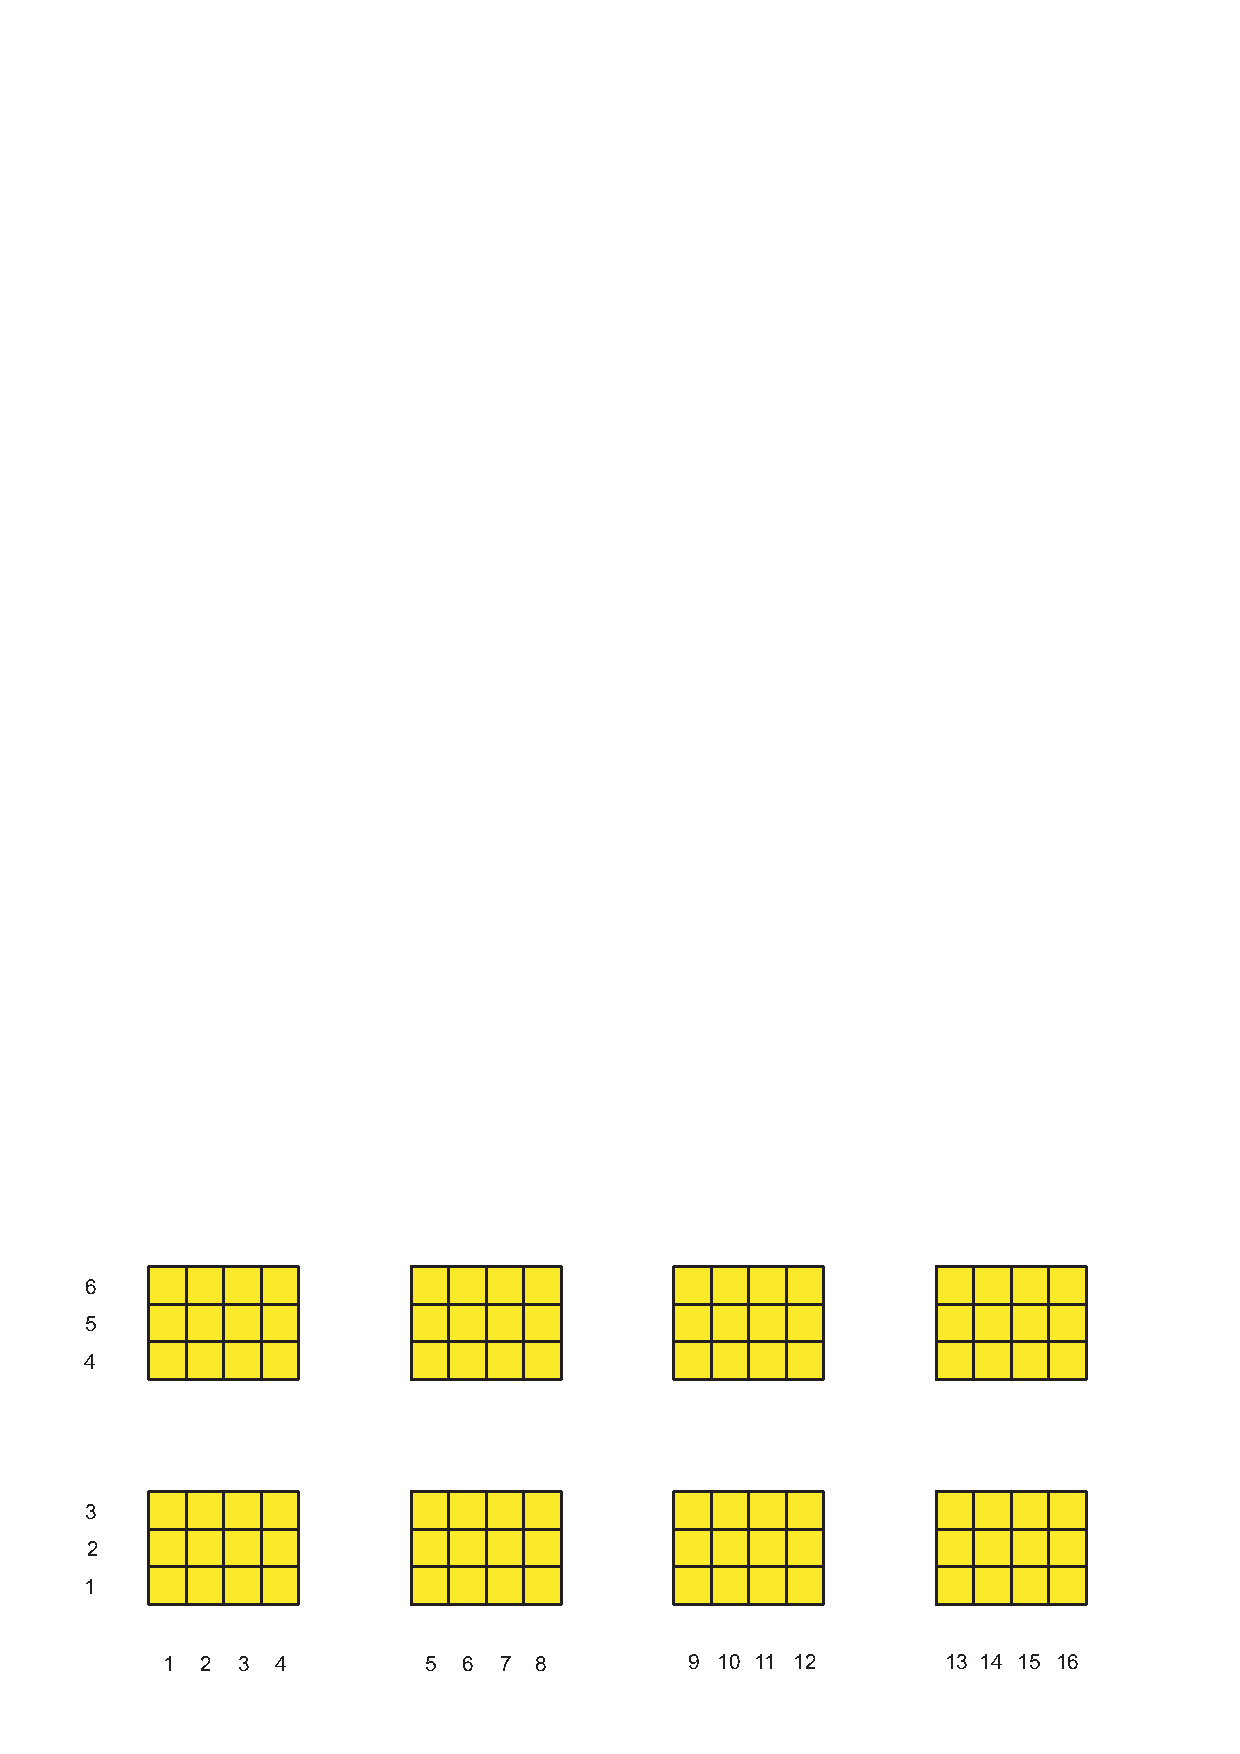
\includegraphics{GridExclusiveReg}}
  \caption{An example of a Grid's exclusive region for the corner stagger}
  \label{fig:gridexreg}
  \end{figure}
  \end{center}
  
   Figure~\ref{fig:gridexreg} shows an example of a Grid exclusive region for the
   {\tt ESMF\_STAGGERLOC\_CORNER} stagger with default
   stagger padding. This exclusive region would be for a Grid generated by either of the
   following calls: 
%/////////////////////////////////////////////////////////////

 \begin{verbatim}
  grid2D=ESMF_GridCreateNoPeriDim(regDecomp=(/2,4/), maxIndex=(/5,15/), &
           indexflag=ESMF_INDEX_GLOBAL, rc=rc)
 
\end{verbatim}
 
%/////////////////////////////////////////////////////////////

 \begin{verbatim}
  grid2D=ESMF_GridCreateNoPeriDim(countsPerDEDim1=(/4,4,4,3/), &
           countsPerDEDim2=(/3,2/), indexflag=ESMF_INDEX_GLOBAL, rc=rc)
 
\end{verbatim}
 
%/////////////////////////////////////////////////////////////

   Each rectangle in this diagram represents a DE and the numbers along the sides
   are the index values of the locations in the DE. Note that the exclusive region
   has one extra index location in each dimension than the number of cells
   because of the padding for the larger corner stagger location.
  
   The computational region is a user-settable region which can be used
   to distinguish a particular area for computation. The Grid doesn't
   currently contain functionality to let the user set the computational
   region so it defaults to the exclusive region. However, if the
   user sets an Array holding different computational bounds into the
   Grid then that Array's computational bounds will be used.
  
   The total region is the outermost boundary of the memory allocated
   on each DE to hold the data for the stagger location on that DE. This region
   can be as small as the exclusive region, but may be larger to
   include space for halos, memory padding, etc. The total region is
   what is enlarged to include space for halos, and the total region
   must be large enough to contain the maximum halo operation on the
   Grid. The Grid doesn't currently contain functionality to let the
   user set the total region so it defaults to the exclusive region.
   However, if the
   user sets an Array holding different total bounds into the
   Grid then that Array's total bounds will be used.
  
   The user can retrieve a set of bounds for each index space region
   described above: exclusive bounds, computational bounds,
   and total bounds. Note that although some of these are similar
   to bounds provided by ESMF\_Array subroutines
   (see Section~\ref{Array_regions_and_default_bounds})
   the format here is different. The Array bounds are only for
   distributed dimensions and are ordered to correspond
   to the dimension order in the associated DistGrid. The bounds
   provided by the Grid are ordered according to the order of dimensions of the data
   in question. This means that the bounds provided should be usable
   "as is" to access the data.
  
   Each of the three types of bounds refers to the maximum and minimum
   per dimension of the index ranges of a particular region. The parameters
   referring to the maximums contain a 'U' for upper. The parameters referring
   to the minimums contain an 'L' for lower. The bounds and associated
   quantities are almost always given on a per DE basis. The three types of
   bounds {\tt exclusiveBounds}, {\tt computationalBounds}, and {\tt totalBounds} refer
   to the ranges of the exclusive region, the computational region, and the
   total region. Each of these bounds also has a corresponding count parameter
   which gives the number of items across that region (on a DE) in each dimension.
   (e.g. {\tt totalCount(d)=totallUBound(i)-totalLBound(i)+1}). Width parameters
   give the spacing between two different types of region. The
   {\tt computationalWidth} argument gives the spacing between the exclusive
   region and the computational region. The {\tt totalWidth} argument gives the
   spacing between the total region and the computational region. Like the
   other bound information these are typically on a per DE basis, for example
   specifying {\tt totalLWidth=(1,1)} makes the bottom of the total
   region one lower in each dimension than the computational region on
   each DE. The exceptions to the per DE rule are
   {\tt staggerEdgeWidth}, and {\tt gridEdgeWidth}
   which give the spacing only on the DEs along the boundary of the Grid.
  
   All the above bound discussions only apply to the grid with non-arbitrary distributions,
   i.e., regular or irregular distributions.  For an arbitrarily distributed grid,
   only center stagger location is supported and there is no padding around the grid.
   Thus, the exclusive bounds, the total bounds and the computational bounds are identical
   and {\tt staggerEdgeWidth}, and {\tt gridEdgeWidth} are all zeros. 
%/////////////////////////////////////////////////////////////

  \subsubsection{Get Grid coordinate bounds}
  
   When operating on coordinates the user may often wish to
   retrieve the bounds of the piece of coordinate data on
   a particular local DE. This is useful for iterating through the
   data to set coordinates, retrieve coordinates, or do calculations.
   The method {\tt ESMF\_GridGetCoord} allows the user
   to retrieve bound information for a particular coordinate
   array.
  
   As described in the previous section there are three types of bounds the user can
   get: exclusive bounds, computational bounds,
   and total bounds. The bounds
   provided by {\tt ESMF\_GridGetCoordBounds} are for both distributed
   and undistributed dimensions and are ordered according to the
   order of dimensions in the  coordinate. This means that the bounds
    provided should be usable
   "as is" to access data in the coordinate array. In the case
   of factorized coordinate Arrays where a coordinate may
   have a smaller dimension than its associated Grid, then
   the dimension of the coordinate's bounds are the dimension of
   the coordinate, not the Grid.
  
   The following is an example of retrieving the bounds for localDE 0 for the first
   coordinate array from the corner stagger location. 
%/////////////////////////////////////////////////////////////

 \begin{verbatim}
   call ESMF_GridGetCoordBounds(grid2D, coordDim=1, localDE=0,  &
          staggerLoc=ESMF_STAGGERLOC_CORNER,                         &
          exclusiveLBound=elbnd, exclusiveUBound=eubnd,              &
          computationalLBound=clbnd, computationalUBound=cubnd,      &
          totalLBound=tlbnd, totalUBound=tubnd, rc=rc)
 
\end{verbatim}
 
%/////////////////////////////////////////////////////////////

  \subsubsection{Get Grid stagger location bounds}
  
   When operating on data stored at a particular stagger
   in a Grid the user may find it useful to be able
   to retrieve the bounds of the data on a particular local DE.
   This is useful for iterating through the
   data for computations or allocating arrays to hold the data.
   The method {\tt ESMF\_GridGet} allows the user
   to retrieve bound information for a particular stagger location.
  
   As described in Section~\ref{sec:grid:usage:bounds} there are three types of bounds
   the user can typically get, however, the Grid doesn't hold data at
   a stagger location (that is the job of the Field), and so
   no Array is contained there and so no total region exists, so the
   user may only retrieve exclusive and computational bounds from
   a stagger location.  The bounds
   provided by {\tt ESMF\_GridGet} are ordered according to the
   order of dimensions in the Grid.
  
   The following is an example of retrieving the bounds for localDE 0
   from the corner stagger location. 
%/////////////////////////////////////////////////////////////

 \begin{verbatim}
   call ESMF_GridGet(grid2D, localDE=0,                         &
          staggerLoc=ESMF_STAGGERLOC_CORNER,                    &
          exclusiveLBound=elbnd, exclusiveUBound=eubnd,         &
          computationalLBound=clbnd, computationalUBound=cubnd, rc=rc)
 
\end{verbatim}
 
%/////////////////////////////////////////////////////////////

  \subsubsection{Get Grid stagger location information}
  
   In addition to the per DE information that can be accessed about
   a stagger location there is some global information that can
   accessed by using {\tt ESMF\_GridGet} without specifying a
   localDE. One of the uses of this information is to create
   an ESMF Array to hold data for a stagger location.
  
   \begin{sloppypar}
   The information currently available from a stagger
   location is the {\tt distgrid}. The {\tt distgrid} gives the
   distgrid which describes the size and distribution of the elements in the stagger location.
   \end{sloppypar}
  
   The following is an example of retrieving information for localDE 0
   from the corner stagger location. 
%/////////////////////////////////////////////////////////////

 \begin{verbatim}
    ! Get info about staggerloc
    call ESMF_GridGet(grid2D, staggerLoc=ESMF_STAGGERLOC_CORNER,  &
           distgrid=staggerDistgrid, &
           rc=rc)

 
\end{verbatim}
 
%/////////////////////////////////////////////////////////////

  \subsubsection{Create an Array at a stagger location}
  
   In order to create an Array to correspond to a Grid stagger location
   several pieces of information need to be obtained from both the
   Grid and the stagger location in the Grid.
  
   The information that needs to be obtained from the Grid
   is the {\tt distgridToGridMap} to ensure that the new Array
   has its  dimensions are mapped correctly to the Grid. These
   are obtained using the {\tt ESMF\_GridGet} method.
  
   The information that needs to be obtained from the stagger
   location is the distgrid that describes the size and distribution
   of the elements in the stagger location. This information can
   be obtained using the stagger location specific {\tt ESMF\_GridGet} method.
  
   The following is an example of using information from a 2D Grid with non-arbitrary
   distribution to create an Array corresponding to a stagger location.
   
%/////////////////////////////////////////////////////////////

 \begin{verbatim}

    ! Get info from Grid
    call ESMF_GridGet(grid2D, distgridToGridMap=distgridToGridMap, rc=rc)
 
\end{verbatim}
 
%/////////////////////////////////////////////////////////////

 \begin{verbatim}

    ! Get info about staggerloc
    call ESMF_GridGet(grid2D, staggerLoc=ESMF_STAGGERLOC_CORNER, &
           distgrid=staggerDistgrid, &
           rc=rc)
 
\end{verbatim}
 
%/////////////////////////////////////////////////////////////

 \begin{verbatim}


    ! construct ArraySpec
    call ESMF_ArraySpecSet(arrayspec, rank=2, typekind=ESMF_TYPEKIND_R8, rc=rc)
 
\end{verbatim}
 
%/////////////////////////////////////////////////////////////

 \begin{verbatim}


    ! Create an Array based on info from grid
    array=ESMF_ArrayCreate(arrayspec=arrayspec, &
            distgrid=staggerDistgrid, distgridToArrayMap=distgridToGridMap, &
            rc=rc)

 
\end{verbatim}
 
%/////////////////////////////////////////////////////////////

   Creating an Array for a Grid with arbitrary distribution is different.
   For a 2D Grid with both dimension arbitrarily distributed, the Array dimension
   is 1.  For a 3D Grid with two arbitrarily distributed dimensions and one
   undistributed dimension, the Array dimension is 2.  In general,
   if the Array does not have any ungridded dimension, the Array dimension
   should be 1 plus the number of undistributed dimensions of the Grid.
  
   The following is an example of creating an Array for a 3D Grid with 2
   arbitrarily distributed dimensions such as the one defined in Section~\ref{example:ArbGridWithUndistDim}. 
%/////////////////////////////////////////////////////////////

 \begin{verbatim}
    ! Get distGrid from Grid
    call ESMF_GridGet(grid3D, distgrid=distgrid, rc=rc)
 
\end{verbatim}
 
%/////////////////////////////////////////////////////////////

 \begin{verbatim}


    ! construct ArraySpec
    call ESMF_ArraySpecSet(arrayspec, rank=2, typekind=ESMF_TYPEKIND_R8, rc=rc)
 
\end{verbatim}
 
%/////////////////////////////////////////////////////////////

 \begin{verbatim}


    ! Create an Array based on the presence of distributed dimensions
    array=ESMF_ArrayCreate(arrayspec=arrayspec,distgrid=distgrid, rc=rc)

 
\end{verbatim}
 
%/////////////////////////////////////////////////////////////

  \subsubsection{Create more complex Grids using DistGrid}
  \label{sec:usage:adv:create}
  
   Besides the shortcut methods for creating a Grid object such as
   {\tt ESMF\_GridCreateNoPeriDim()}, there is
   a set of methods which give the user more control over the
   specifics of the grid.  The following describes the more
   general interface, using DistGrid.
   The basic idea is to first create an ESMF DistGrid object describing
   the distribution and shape of the Grid, and then to employ that to either directly
   create the Grid or first create Arrays and then create the Grid from those.
   This method gives the user maximum control over the topology and distribution of the Grid.
   See the DistGrid documentation in Section~\ref{sec:DistGrid} for an
   in-depth description of its interface and use.
  
   As an example, the following call constructs
   a 10x20 Grid with a lower bound of (1,2). 
%/////////////////////////////////////////////////////////////

 \begin{verbatim}
   ! Create DistGrid
   distgrid2D = ESMF_DistGridCreate(minIndex=(/1,2/), maxIndex=(/11,22/), &
           rc=rc)
 
\end{verbatim}
 
%/////////////////////////////////////////////////////////////

 \begin{verbatim}

   ! Create Grid
   grid3D=ESMF_GridCreate(distGrid=distgrid2D, rc=rc)
 
\end{verbatim}
 
%/////////////////////////////////////////////////////////////

   \begin{sloppypar}
   To alter which dimensions are distributed, the {\tt distgridToGridMap}
   argument can be used. The {\tt distgridToGridMap} is used to set
   which dimensions of the Grid are mapped to the dimensions
   described by {\tt maxIndex}. In other words, it describes how the dimensions of
   the underlying default DistGrid are mapped to the Grid. Each entry
   in {\tt distgridToGridMap} contains the Grid dimension to which the corresponding
   DistGrid dimension should be mapped.
   The following example illustrates the creation of a Grid where the largest
   dimension is first. To accomplish this the two dimensions are swapped.
   \end{sloppypar} 
%/////////////////////////////////////////////////////////////

 \begin{verbatim}
   ! Create DistGrid
   distgrid2D = ESMF_DistGridCreate(minIndex=(/1,2/), maxIndex=(/11,22/), &
        rc=rc)
 
\end{verbatim}
 
%/////////////////////////////////////////////////////////////

 \begin{verbatim}

   ! Create Grid
   grid2D=ESMF_GridCreate(distGrid=distgrid2D, distgridToGridMap=(/2,1/), &
        rc=rc)
 
\end{verbatim}
 
%/////////////////////////////////////////////////////////////

  \subsubsection{Specify custom stagger locations}
  \label{sec:usage:staggerloc:adv}
  
   Although ESMF provides a set of predefined stagger locations (See Section~\ref{const:staggerloc}),
   the user may need one outside this set. This section describes the construction of
   custom stagger locations.
  
   To completely specify a stagger for an arbitrary number of dimensions, we define the
   stagger location in terms of a set of cartesian coordinates. The cell is represented
   by a n-dimensional cube with sides of length 2, and the coordinate origin located at
   the center of the cell. The geometry of the cell is for reference purposes only,
   and does not literally represent the actual shape of the cell. Think of this method
   instead as an easy way to specify a part (e.g. center, corner, face) of a higher
   dimensional cell which is extensible to any number of dimensions.
  
   To illustrate this approach, consider a 2D cell. In 2 dimensions
   the cell is represented by a square. An xy axis is placed at its center, with the
   positive x-axis oriented {\em East} and the positive y-axis oriented {\em North}.
   The resulting coordinate for the lower left corner is at $(-1,-1)$, and upper right
   corner at $(1,1)$.
   However, because our staggers are symmetric they don't need to distinguish between
   the $-1$, and the $1$, so we only need to concern ourselves with the first quadrant of
   this cell. We only need to use the $1$, and the $0$, and many of the cell locations
   collapse together (e.g. we only need to represent one corner). See figure~\ref{fig:gridcuststaggerloc}
   for an illustration of these concepts.
  
  \begin{center}
  \begin{figure}
  \center
  \scalebox{0.75}{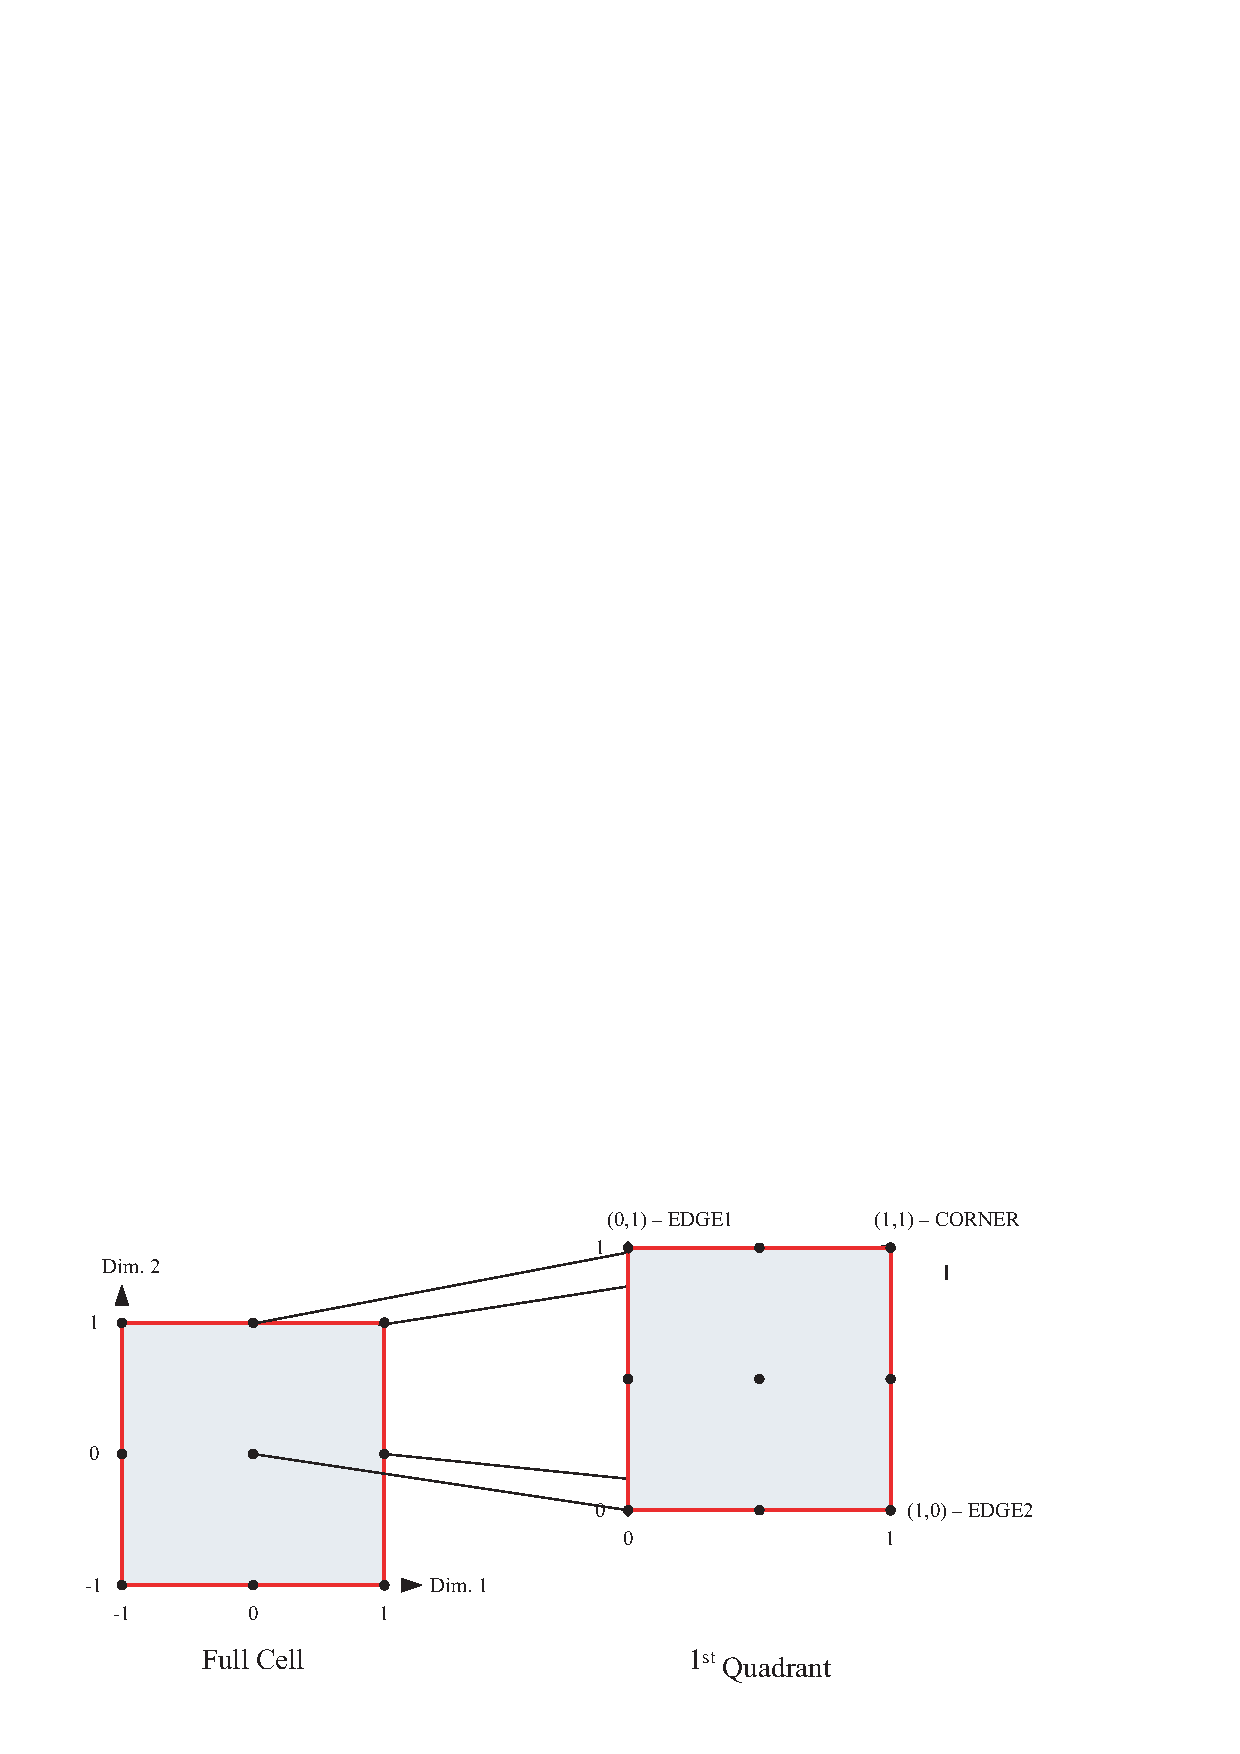
\includegraphics{GridCustStaggerLoc}}
  \caption{An example of specifying 2D stagger locations using coordinates.}
  \label{fig:gridcuststaggerloc}
  \end{figure}
  \end{center}
  
   The cell center is represented by the coordinate pair $(0,0)$ indicating the origin.
   The cell corner is $+1$ in each direction, giving a coordinate pair of $(1,1)$.
   The edges are each $+1$ in one dimension and $0$ in the other indicating that
   they're even with the center in one dimension and offset in the other.
  
   For three dimensions, the vertical component of the stagger location can be added by
   simply adding an additional coordinate. The three dimensional generalization of the
   cell center becomes $(0,0,0)$ and the cell corner becomes $(1,1,1)$. The rest of
   the 3D stagger locations are combinations of $+1$ offsets from the center.
  
   To generalize this to $d$ dimensions, to represent a $d$ dimensional stagger
   location. A set of $d$ $0$ and $1$ is used to specify for each dimension
   whether a stagger location is aligned with the cell center in that dimension ($0$),
   or offset by $+1$ in that dimension ($1$). Using this scheme we can represent
   any symmetric stagger location.
  
   To construct a custom stagger location in ESMF the subroutine
   {\tt ESMF\_StaggerLocSet()} is used to specify,
   for each dimension, whether the stagger is located at the interior (0)
   or on the boundary (1) of the cell. This method allows users
   to construct stagger locations for which
   there is no predefined value. In this example, it's used to
   set the 4D center and 4D corner locations.
   
%/////////////////////////////////////////////////////////////

 \begin{verbatim}

   ! Set Center
   call ESMF_StaggerLocSet(staggerLoc,loc=(/0,0,0,0/),rc=rc)
 
\end{verbatim}
 
%/////////////////////////////////////////////////////////////

 \begin{verbatim}
   call ESMF_GridAddCoord(grid4D, staggerLoc=staggerLoc, rc=rc)
 
\end{verbatim}
 
%/////////////////////////////////////////////////////////////

 \begin{verbatim}


   ! Set Corner
   call ESMF_StaggerLocSet(staggerLoc,loc=(/1,1,1,1/),rc=rc)
 
\end{verbatim}
 
%/////////////////////////////////////////////////////////////

 \begin{verbatim}

   call ESMF_GridAddCoord(grid4D, staggerLoc=staggerLoc, rc=rc)
 
\end{verbatim}
 
%/////////////////////////////////////////////////////////////

  \subsubsection{Specify custom stagger padding}
  \label{sec:usage:staggerpadding:adv}
  
  There is an added complication with the data (e.g. coordinates) stored at stagger locations in
  that they can require different amounts of storage depending
  on the underlying Grid type.
  
  \begin{center}
  \begin{figure}
  \center
  \scalebox{0.75}{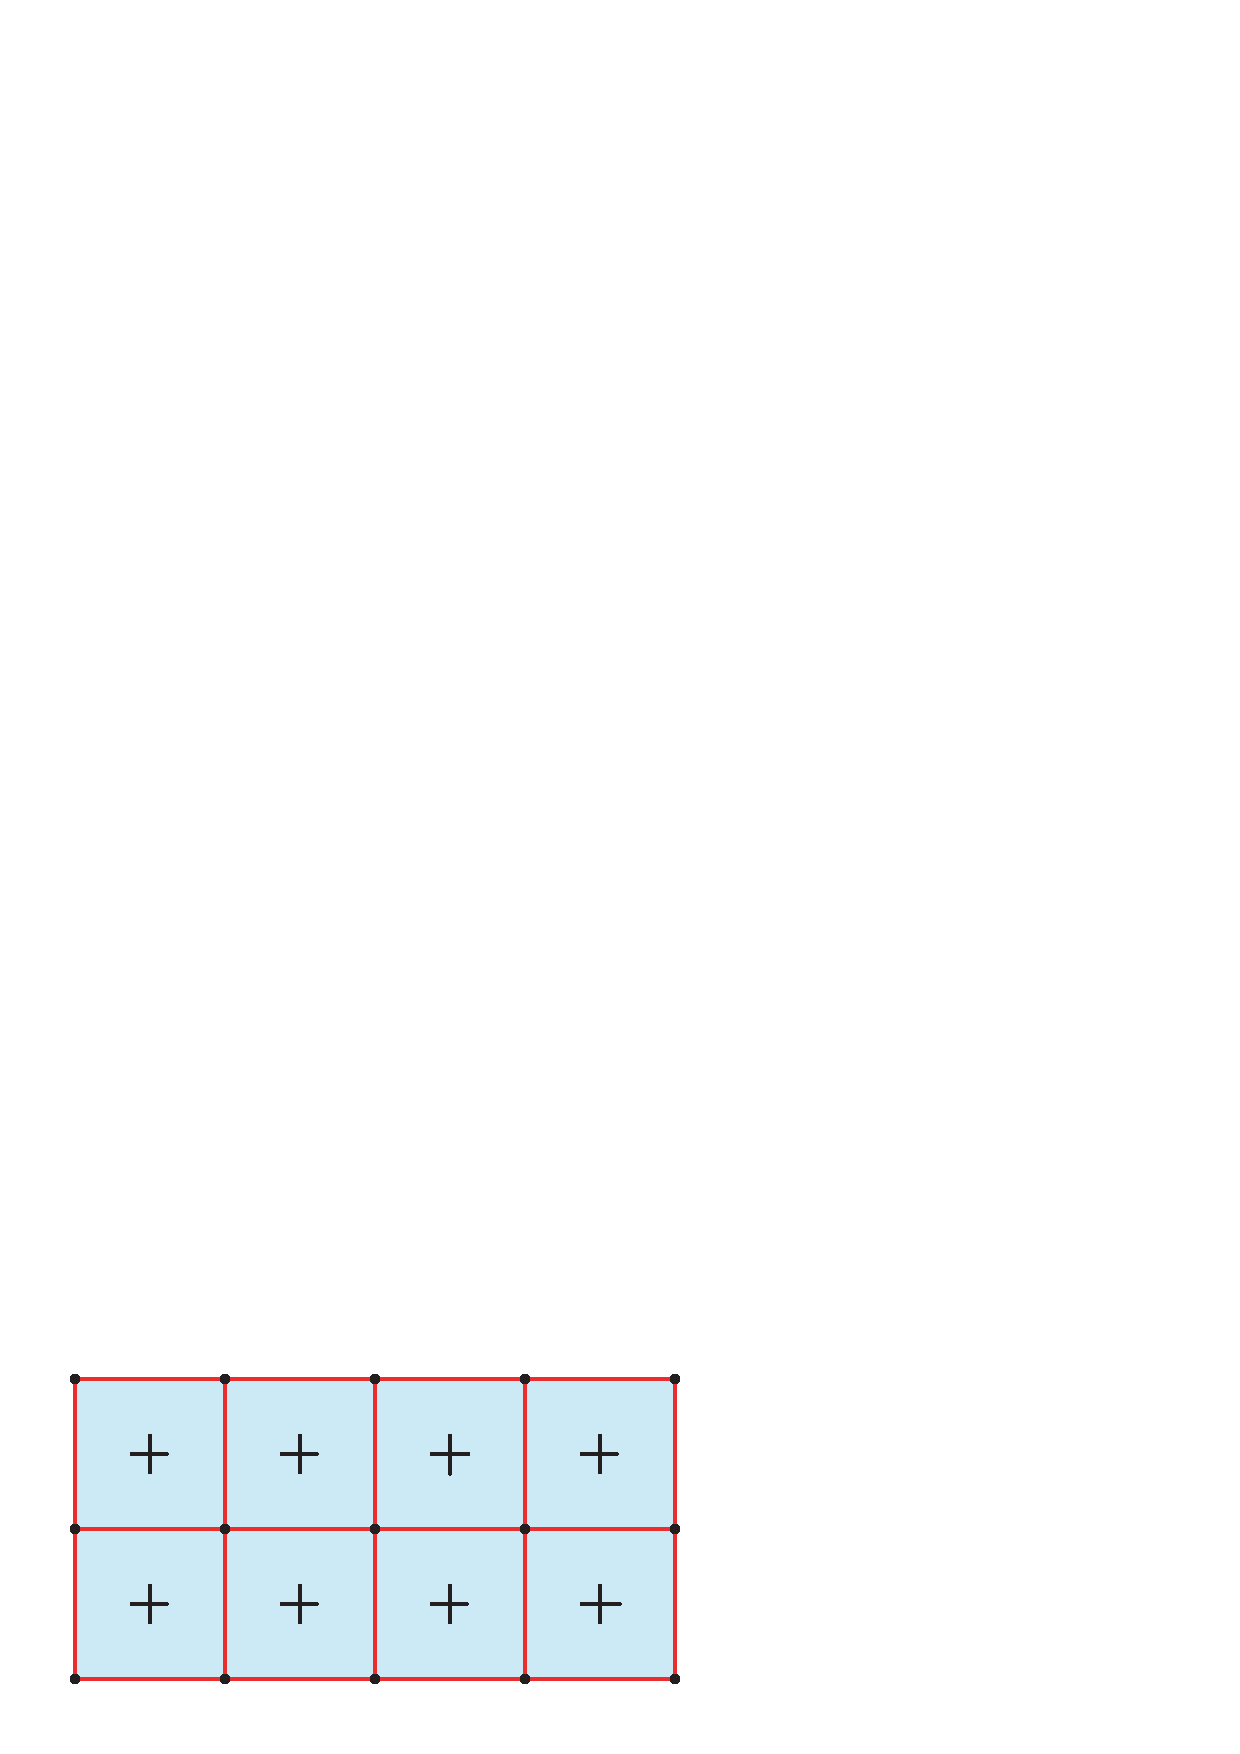
\includegraphics{GridCellsAndCorners}}
  \caption{An example 2D Grid with cell centers and corners.}
  \label{fig:gridcellsandcorners}
  \end{figure}
  \end{center}
  
   Consider the example 2D grid in figure~\ref{fig:gridcellsandcorners}, where the dots represent the cell corners
   and the ``+'' represents the cell centers. For the corners to completely
   enclose the cell centers (symmetric stagger), the number of corners in each
   dimension needs to be one greater then the number of cell centers. In the above
   figure, there are two rows and three columns of cell centers. To enclose the
   cell centers, there must be three rows and four columns of cell corners.
   This is true in general for Grids without periodicity or
   other connections.  In fact, for a symmetric stagger, given that the center
   location requires n x m storage, the corresponding corner location
   requires n+1 x m+1, and the edges, depending on the side, require n+1 x m or
   m+1 x n.  In order to add the extra storage, a new DistGrid is
   created at each stagger location. This Distgrid is similar to the DistGrid
   used to create the Grid, but has an extra set of elements added to hold the
   index locations for the stagger padding.
   By default, when the coordinate arrays are created, one extra
   layer of padding is added to the index space to create symmetric staggers
   (i.e. the center location is surrounded). The default is to add this padding
   on the positive side, and to only add this padding where needed
   (e.g. no padding for the center, padding
   on both dimensions for the corner, in only one dimension for the
   edge in 2D.) There are two ways for the user to change
   these defaults.
  
   One way is to use the {\tt GridEdgeWidth} or {\tt GridAlign} arguments
   when creating a Grid. These arguments can be used to change the default padding
   around the Grid cell index space. This extra padding is used by default
   when setting the padding for a stagger location.
  
   The {\tt gridEdgeLWidth} and
   {\tt gridEdgeUWidth} arguments are both 1D arrays of the
   same size as the Grid dimension. The entries in the arrays
   give the extra offset from the outer boundary of
   the grid cell index space. The following example shows the
   creation of a Grid with all the extra space to hold stagger padding
   on the negative side of a Grid. This is the reverse of
   the default behavior. The resulting Grid will have
   an exclusive region which extends from $(-1,-1)$ to
   $(10,10)$, however, the cell center stagger location
   will still extend from $(1,1)$ to $(10,10)$. 
%/////////////////////////////////////////////////////////////

 \begin{verbatim}
   grid2D=ESMF_GridCreateNoPeriDim(minIndex=(/1,1/),maxIndex=(/10,10/), &
            gridEdgeLWidth=(/1,1/), gridEdgeUWidth=(/0,0/), rc=rc)

 
\end{verbatim}
 
%/////////////////////////////////////////////////////////////

   To indicate how the data in a Grid's stagger locations are aligned with the
   cell centers, the optional {\tt gridAlign} parameter
   may be used. This parameter indicates which stagger elements
   in a cell share the same index values as the cell center.
   For example, in a 2D cell, it would indicate which of the four corners has
   the same index value as the center. To set {\tt gridAlign},
   the values -1,+1 are used to indicate the alignment in
   each dimension. This parameter is mostly
   informational, however, if the {\tt gridEdgeWidth} parameters
   are not set then its value determines where the default padding
   is placed. If not specified, then the default is to align all
   staggers to the most negative, so the padding is on the positive side.
   The following code illustrates creating a Grid aligned to the reverse of
   default (with everything to the positive side). This creates a
   Grid identical to that created in the previous example. 
%/////////////////////////////////////////////////////////////

 \begin{verbatim}
   grid2D=ESMF_GridCreateNoPeriDim(minIndex=(/1,1/),maxIndex=(/10,10/), &
            gridAlign=(/1,1/), rc=rc)

 
\end{verbatim}
 
%/////////////////////////////////////////////////////////////

   The {\tt gridEdgeWidth} and {\tt gridAlign} arguments both
   allow the user to set the default padding to be used
   by stagger locations in a Grid. By default, stagger locations
   allocated in a Grid set their stagger padding based on these
   values.  A stagger location's padding in each dimension is
   equal to the value of {\tt gridEdgeWidth} (or the value implied
   by {\tt gridAlign}), unless the stagger location is centered
   in a dimension in which case the stagger padding is 0. For example,
   the cell center stagger location has 0 stagger padding in all
   dimensions, whereas the edge stagger location lower padding
   is equal to {\tt gridEdgeLWidth} and the upper padding is equal
   to {\tt gridEdgeUWidth} in one dimension, but both are 0 in the other,
   centered, dimension.  If the user wishes to set the stagger padding
   individually for each stagger location they may use the
   {\tt staggerEdgeWidth} and {\tt staggerAlign} arguments.
  
   The {\tt staggerEdgeLWidth} and
   {\tt staggerEdgeUWidth} arguments are both 1D arrays of the
   same size as the Grid dimension. The entries in the arrays
   give the extra offset from the Grid cell index space
   for a stagger location. The following example shows the
   addition of two stagger locations. The
   corner location has no extra boundary and the
   center has a single layer of extra padding on
   the negative side and none on the positive.  This is the reverse of
   the default behavior. 
%/////////////////////////////////////////////////////////////

 \begin{verbatim}
   grid2D=ESMF_GridCreate(distgrid=distgrid2D, &
            gridEdgeLWidth=(/1,1/), gridEdgeUWidth=(/0,0/), rc=rc)
 
\end{verbatim}
 
%/////////////////////////////////////////////////////////////

 \begin{verbatim}


   call ESMF_GridAddCoord(grid2D, &
          staggerLoc=ESMF_STAGGERLOC_CORNER, &
          staggerEdgeLWidth=(/0,0/), staggerEdgeUWidth=(/0,0/), rc=rc)
 
\end{verbatim}
 
%/////////////////////////////////////////////////////////////

 \begin{verbatim}


   call ESMF_GridAddCoord(grid2D, &
          staggerLoc=ESMF_STAGGERLOC_CENTER, &
          staggerEdgeLWidth=(/1,1/), staggerEdgeUWidth=(/0,0/), rc=rc)

 
\end{verbatim}
 
%/////////////////////////////////////////////////////////////

   To indicate how the data at a particular stagger location is aligned with the
   cell center, the optional {\tt staggerAlign} parameter
   may be used. This parameter indicates which stagger elements
   in a cell share the same index values as the cell center.
   For example, in a 2D cell, it would indicate which of the four corners has
   the same index value as the center. To set {\tt staggerAlign},
   the values -1,+1 are used to indicate the alignment in
   each dimension. If a stagger location is
   centered in a dimension (e.g. an edge in 2D), then that
   dimension is ignored in the alignment. This parameter is mostly
   informational, however, if the {\tt staggerEdgeWidth} parameters
   are not set then its value determines where the default padding
   is placed. If not specified, then the default is to align all
   staggers to the most negative, so the padding is on the positive side.
   The following code illustrates aligning the positive (northeast in 2D)
   corner with the center. 
%/////////////////////////////////////////////////////////////

 \begin{verbatim}
   call ESMF_GridAddCoord(grid2D, &
          staggerLoc=ESMF_STAGGERLOC_CORNER, staggerAlign=(/1,1/), rc=rc)
 
\end{verbatim}

%...............................................................
\setlength{\parskip}{\oldparskip}
\setlength{\parindent}{\oldparindent}
\setlength{\baselineskip}{\oldbaselineskip}

%%                **** IMPORTANT NOTICE *****
% This LaTeX file has been automatically produced by ProTeX v. 1.1
% Any changes made to this file will likely be lost next time
% this file is regenerated from its source. Send questions 
% to Arlindo da Silva, dasilva@gsfc.nasa.gov
 
\setlength{\oldparskip}{\parskip}
\setlength{\parskip}{1.5ex}
\setlength{\oldparindent}{\parindent}
\setlength{\parindent}{0pt}
\setlength{\oldbaselineskip}{\baselineskip}
\setlength{\baselineskip}{11pt}
 
%--------------------- SHORT-HAND MACROS ----------------------
\def\bv{\begin{verbatim}}
\def\ev{\end{verbatim}}
\def\be{\begin{equation}}
\def\ee{\end{equation}}
\def\bea{\begin{eqnarray}}
\def\eea{\end{eqnarray}}
\def\bi{\begin{itemize}}
\def\ei{\end{itemize}}
\def\bn{\begin{enumerate}}
\def\en{\end{enumerate}}
\def\bd{\begin{description}}
\def\ed{\end{description}}
\def\({\left (}
\def\){\right )}
\def\[{\left [}
\def\]{\right ]}
\def\<{\left  \langle}
\def\>{\right \rangle}
\def\cI{{\cal I}}
\def\diag{\mathop{\rm diag}}
\def\tr{\mathop{\rm tr}}
%-------------------------------------------------------------

\markboth{Left}{Source File: ESMF\_GridCreateRegFromDGEx.F90,  Date: Tue May  5 20:59:48 MDT 2020
}

 
%/////////////////////////////////////////////////////////////

   \subsubsection{Create a 2D Grid with regular distribution from a DistGrid}~\label{sec:usage:ex:adv:reg}
  
   This example illustrates the creation of a single tile 2D Grid
   with a regular distribution from a DistGrid.  The size of the Grid is
   gridSize(1) by gridSize(2) elements. It only contains data
   in the center stagger location (i.e. Arakawa A-Grid). 
%/////////////////////////////////////////////////////////////

 \begin{verbatim}
      ! Use ESMF framework module
      use ESMF
      use ESMF_TestMod
      implicit none

      ! Local variables  
      integer:: rc, finalrc, result
      type(ESMF_VM):: vm
      type(ESMF_DistGrid) :: distgrid2D
      type(ESMF_Grid) :: grid2D
 
\end{verbatim}
 
%/////////////////////////////////////////////////////////////

   First construct a single tile distgrid with regular distribution of the
   appropriate size. 
%/////////////////////////////////////////////////////////////

 \begin{verbatim}

      distgrid2D = ESMF_DistGridCreate(minIndex=(/1,1/),      &
                          maxIndex=(/20,30/), rc=rc)  
 
\end{verbatim}
 
%/////////////////////////////////////////////////////////////

      Create a Grid using the distgrid.  
%/////////////////////////////////////////////////////////////

 \begin{verbatim}
     Grid2D=ESMF_GridCreate(name="Simple 2D Regular", &
               distgrid=distgrid2D, rc=rc)
 
\end{verbatim}
 
%/////////////////////////////////////////////////////////////

   Set the one stagger location as center.  
%/////////////////////////////////////////////////////////////

 \begin{verbatim}
   call ESMF_GridAddCoord(Grid2D,  &
          staggerLoc=ESMF_STAGGERLOC_CENTER, rc=rc)
 
\end{verbatim}

%...............................................................
\setlength{\parskip}{\oldparskip}
\setlength{\parindent}{\oldparindent}
\setlength{\baselineskip}{\oldbaselineskip}

%%                **** IMPORTANT NOTICE *****
% This LaTeX file has been automatically produced by ProTeX v. 1.1
% Any changes made to this file will likely be lost next time
% this file is regenerated from its source. Send questions 
% to Arlindo da Silva, dasilva@gsfc.nasa.gov
 
\setlength{\oldparskip}{\parskip}
\setlength{\parskip}{1.5ex}
\setlength{\oldparindent}{\parindent}
\setlength{\parindent}{0pt}
\setlength{\oldbaselineskip}{\baselineskip}
\setlength{\baselineskip}{11pt}
 
%--------------------- SHORT-HAND MACROS ----------------------
\def\bv{\begin{verbatim}}
\def\ev{\end{verbatim}}
\def\be{\begin{equation}}
\def\ee{\end{equation}}
\def\bea{\begin{eqnarray}}
\def\eea{\end{eqnarray}}
\def\bi{\begin{itemize}}
\def\ei{\end{itemize}}
\def\bn{\begin{enumerate}}
\def\en{\end{enumerate}}
\def\bd{\begin{description}}
\def\ed{\end{description}}
\def\({\left (}
\def\){\right )}
\def\[{\left [}
\def\]{\right ]}
\def\<{\left  \langle}
\def\>{\right \rangle}
\def\cI{{\cal I}}
\def\diag{\mathop{\rm diag}}
\def\tr{\mathop{\rm tr}}
%-------------------------------------------------------------

\markboth{Left}{Source File: ESMF\_GridCreateTripoleEx.F90,  Date: Tue May  5 20:59:48 MDT 2020
}

 
%/////////////////////////////////////////////////////////////

   \subsubsection{Create a 2D tripole grid from Arrays}\label{sec:usage:ex:adv:tripole}
  
   This example illustrates the creation of a 2D tripole Grid from coordinate data
   read in on a single processor and then distributed to the rest of the processors. 
   The Grid contains just the center stagger location. The size of the Grid is gridSize(1) by 
   gridSize(2). 
%/////////////////////////////////////////////////////////////

 \begin{verbatim}
      ! Use ESMF framework module
      use ESMF
      implicit none

      ! Local variables  
      integer:: rc, finalrc
      integer:: myPet, npets, rootPet
      type(ESMF_VM):: vm
      type(ESMF_Config) :: config
      type(ESMF_DistGrid) :: distgrid
      type(ESMF_Array) :: gridCoordArrays(2,1)
      type(ESMF_Array) :: gridCntrCoordArrayLat,gridCntrCoordArrayLon
      type(ESMF_StaggerLoc) :: staggerLocs(1)
      type(ESMF_ArraySpec) ::  arrayspec
      real(ESMF_KIND_R8), allocatable :: globalGridCntrCoordLat(:,:)
      real(ESMF_KIND_R8), allocatable :: globalGridCntrCoordLon(:,:)
      integer :: gridSize(2), gridRank
      integer, allocatable ::  connectionList(:,:)
 
\end{verbatim}
 
%/////////////////////////////////////////////////////////////

   Allocate a Fortran array to hold sphere coodinates, then read them in. This
   all takes place on one processor. Later the data will be distributed across the processors.  
%/////////////////////////////////////////////////////////////

 \begin{verbatim}
      gridRank=2  ! 2D grid
      call read2Dgriddata(gridSize)
      allocate( globalGridCntrCoordLat(gridSize(1),gridSize(2)))
      allocate( globalGridCntrCoordLon(gridSize(1),gridSize(2)))
      call read2Dgrid(globalGridCntrCoordLat)
      call read2Dgrid(globalGridCntrCoordLon)
 
\end{verbatim}
 
%/////////////////////////////////////////////////////////////

   Construct a single tile tripole domain. 
   Specify that the first dimension is periodic: \\
  
   \begin{itemize}
   \item Setting tileIndexA=tileIndexB indicates that the connection 
        is within the tile.
   \item The position vector is set to span the width of the tile's 
        first dimension.
   \item The repetitionVector indicates that the connection repeats along
             the dimension. This takes care of both sides of the connection.
   \end{itemize} 
%/////////////////////////////////////////////////////////////

 \begin{verbatim}

      allocate( connectionList(2*gridRank,3) )
      call ESMF_ConnectionElementConstruct(                          &
                 connectionElement=connectionList(:,1),     &
                 tileIndexA=1, tileIndexB=1,              &
                 positionVector = (/gridSize(1),0/),        &
                 repetitionVector= (/1,0/), rc=rc)
 
\end{verbatim}
 
%/////////////////////////////////////////////////////////////

   Specify the northern bipolar fold: \\
  
    The position and orientation vectors indicate that each element 
    along the top edge of the tile is attached to the corresponding
    element across the fold.  
%/////////////////////////////////////////////////////////////

 \begin{verbatim}
       call ESMF_ConnectionElementConstruct(
                  connectionElement = connectionList(:,2), &
                  tileIndexA = 1, tileIndexB = 1, &
                  positionVector = (/gridSize(1)+1, 2*gridSize(2)/), &
                  orientationVector = (/-1, -2/), &
                  rc=rc)
 
\end{verbatim}
 
%/////////////////////////////////////////////////////////////

   Specify the south pole: \\
  
    The position and orientation vectors indicate that each element along
     the bottom edge of the tile is attached to the element directly across the pole.  
%/////////////////////////////////////////////////////////////

 \begin{verbatim}
       call ESMF_ConnectionElementConstruct( 
                 connectionElement = connectionList(:,3), &
                 tileIndexA = 1, tileIndexB = 1, &
                 positionVector = (/gridSize(1)/2, 0/), &
                 orientationVector = (/1, -2/), &
                 repetitionVector = (/1, 0/), &
                 rc=rc)
 
\end{verbatim}
 
%/////////////////////////////////////////////////////////////

    Construct distgrid from connection information. 
%/////////////////////////////////////////////////////////////

 \begin{verbatim}
      distgrid = ESMF_DistGridCreate( minCorner=(/1,1/),  &
                          maxCorner=(/gridSize(1),gridSize(2)/),    &
                          connectionList=connectionList, rc=rc)  

      deallocate( connectionList )
 
\end{verbatim}
 
%/////////////////////////////////////////////////////////////

    Create an array into which to put the spherical coordinates.
  
%/////////////////////////////////////////////////////////////

 \begin{verbatim}
      call ESMF_ArraySpecSet(arrayspec, typekind=ESMF_TYPEKIND_R8,  &
                 rank=gridRank)

      gridCntrCoordArrayLat = ESMF_ArrayCreate(arrayspec=arrayspec,  &
                                                 distgrid=distgrid, rc=rc)
      gridCntrCoordArrayLon = ESMF_ArrayCreate(arrayspec=arrayspec, &
                                                 distgrid=distgrid, rc=rc)
 
\end{verbatim}
 
%/////////////////////////////////////////////////////////////

    Scatter the Fortran array according to DistGrid into the esmf Array. 
%/////////////////////////////////////////////////////////////

 \begin{verbatim}
      call ESMF_ArrayScatter(gridCntrCoordArrayLat, globalGridCntrCoordLat, &
                rootPet=rootPet, vm=vm, rc=rc)    

      call ESMF_ArrayScatter(gridCntrCoordArrayLon, globalGridCntrCoordLon, &
                rootPet=rootPet, vm=vm, rc=rc)    
 
\end{verbatim}
 
%/////////////////////////////////////////////////////////////

   Load Stagger location and corresponding coordinate arrays into array of ESMF Arrays. 
%/////////////////////////////////////////////////////////////

 \begin{verbatim}
     staggerlocs(1)=ESMF_STAGGERLOC_CENTER
     gridCoordArrays(1,1)=gridCntrCoordArrayLon     
     gridCoordArrays(2,1)=gridCntrCoordArrayLat     
 
\end{verbatim}
 
%/////////////////////////////////////////////////////////////

      Create a Grid from the coordinate array.  
%/////////////////////////////////////////////////////////////

 \begin{verbatim}
     tripoleGrid = ESMF_GridCreate(arrays=gridCoordArrays, &
                               staggerLocs=staggerlocs,rc=rc)
 
\end{verbatim}

%...............................................................
\setlength{\parskip}{\oldparskip}
\setlength{\parindent}{\oldparindent}
\setlength{\baselineskip}{\oldbaselineskip}

%\input{../Infrastructure/Grid/doc/ESMF_GridCreateSph2Dplus1Ex_fapi}
%%                **** IMPORTANT NOTICE *****
% This LaTeX file has been automatically produced by ProTeX v. 1.1
% Any changes made to this file will likely be lost next time
% this file is regenerated from its source. Send questions 
% to Arlindo da Silva, dasilva@gsfc.nasa.gov
 
\setlength{\oldparskip}{\parskip}
\setlength{\parskip}{1.5ex}
\setlength{\oldparindent}{\parindent}
\setlength{\parindent}{0pt}
\setlength{\oldbaselineskip}{\baselineskip}
\setlength{\baselineskip}{11pt}
 
%--------------------- SHORT-HAND MACROS ----------------------
\def\bv{\begin{verbatim}}
\def\ev{\end{verbatim}}
\def\be{\begin{equation}}
\def\ee{\end{equation}}
\def\bea{\begin{eqnarray}}
\def\eea{\end{eqnarray}}
\def\bi{\begin{itemize}}
\def\ei{\end{itemize}}
\def\bn{\begin{enumerate}}
\def\en{\end{enumerate}}
\def\bd{\begin{description}}
\def\ed{\end{description}}
\def\({\left (}
\def\){\right )}
\def\[{\left [}
\def\]{\right ]}
\def\<{\left  \langle}
\def\>{\right \rangle}
\def\cI{{\cal I}}
\def\diag{\mathop{\rm diag}}
\def\tr{\mathop{\rm tr}}
%-------------------------------------------------------------

\markboth{Left}{Source File: ESMF\_GridCreateFromF90ArraysEx.F90,  Date: Tue May  5 20:59:48 MDT 2020
}

 
%/////////////////////////////////////////////////////////////

   \subsubsection{Create a Grid from existing F90 arrays}~\label{sec:example5}
  
   This example illustrates the creation of a simple 2D Grid from coordinate data
    contained in fortan arrays.  The new Grid contains just the center stagger location.
    Each processor contains a pair of 10x10 Fortran 90 arrays named fptrX and fptrY.
    These arrays contain the coordinates for the piece of the global Grid held by each
    processor. The final global Grid will be 20x20 and the pieces of this Grid held
   by each processor are as follows:
  
   \begin{verbatim}
  
    
         20  +--------------+--------------+
             |              |              |                       
             |              |              |                       
             |     PET3     |     PET4     |                       
             |              |              |                       
             |              |              |  
         10  +--------------+--------------+ 
             |              |              |                       
             |              |              |                       
             |     PET 1    |     PET2     |                       
             |              |              |  
             |              |              |                      
          1  +--------------+--------------+
             1             10             20  
  
  
   \end{verbatim}
  
     As illustrated by the diagram, the arrays on processor 1 hold piece (1,1)-(10,10) of the 
     global index space. The arrays on processor 2 hold piece (11,1)-(20,10). The arrays on 
     processor 3 hold piece (1,11)-(10,20), and the arrays on processor 4 hold piece (11,11)-(20,20).
   
%/////////////////////////////////////////////////////////////

 \begin{verbatim}
      ! Use ESMF framework module
      use ESMF
      implicit none

      ! Local variables  
      integer:: rc, finalrc
      integer:: myPet, npets, rootPet
      type(ESMF_VM):: vm
      type(ESMF_Config) :: config
      type(ESMF_DistGrid) :: distgrid
      type(ESMF_Array) :: gridCoordArrays(1,1)
      type(ESMF_StaggerLoc) :: staggerLocs(1)
      type(ESMF_ArraySpec) ::  arrayspec
      real(ESMF_KIND_R8), pointer :: fptrX(:,:),fptrY(:,:)
      integer  ::  deBlockList(2,3,4)
      integer :: petList(4)
 
\end{verbatim}
 
%/////////////////////////////////////////////////////////////

   Create a distgrid to describe how the arrays are to be joined together into the
   global Grid. The {\it deBlockList} actually describes the location of
   DEs, but the default mapping between PETs and DEs is DE m <-> PET m, so
   this is essentially the same thing (assuming the number of PETs and DEs is the 
   same). 
%/////////////////////////////////////////////////////////////

 \begin{verbatim}

      ! Describe how DEs are arranged
      deBlockList(:,1,1)  = (/1,1/)   ! min corner of PET 1
      deBlockList(:,2,1)  = (/1,10/) ! max corner of PET 1
      deBlockList(:,1,2)  = (/1,11/)   ! min corner of PET 2
      deBlockList(:,2,2)  = (/1,20/)  ! max corner of PET 2
      deBlockList(:,1,3)  = (/11,1/)   ! min corner of PET 3
      deBlockList(:,2,3)  = (/11,10/)  ! max corner of PET 3
      deBlockList(:,1,4)  = (/11,11/)   ! min corner of PET 4
      deBlockList(:,2,4)  = (/11,20/)  ! max corner of PET 4
      
      ! Construct distgrid
      distgrid = ESMF_DistGridCreate( minCorner=(/1,1/),  &
                          maxCorner=(/20,20/),    &
                          deBlockList=deBlockList, rc=rc)  

 
\end{verbatim}
 
%/////////////////////////////////////////////////////////////

    Create coordinate arrays from the fortan pointers and the distgrid.
  
%/////////////////////////////////////////////////////////////

 \begin{verbatim}
      gridCoordArrays(1,1)=ESMF_ArrayCreate(fptrX,  &
                             distgrid=distgrid, rc=rc)

      gridCoordArrays(1,2)=ESMF_ArrayCreate(fptrY,  &
                             distgrid=distgrid, rc=rc)

 
\end{verbatim}
 
%/////////////////////////////////////////////////////////////

   Load Stagger location corresponding to coordinate arrays. 
%/////////////////////////////////////////////////////////////

 \begin{verbatim}
     staggerlocs(1)=ESMF_STAGGERLOC_CENTER
 
\end{verbatim}
 
%/////////////////////////////////////////////////////////////

      Create a Grid from the coordinate arrays and the stagger location.  
%/////////////////////////////////////////////////////////////

 \begin{verbatim}
     tileGrid = ESMF_GridCreate(arrays=gridCoordArrays, &
                               staggerLocs=staggerlocs,rc=rc)
 
\end{verbatim}

%...............................................................
\setlength{\parskip}{\oldparskip}
\setlength{\parindent}{\oldparindent}
\setlength{\baselineskip}{\oldbaselineskip}

\subsection{Restrictions and Future Work}
% $Id$

%\subsubsection{Restrictions and Future Work}

\begin{itemize}

\item {\bf 7D limit.}  Only grids up to 7D will be supported.

\item {\bf During the first development phase only single
tile grids are supported.}  In the near future, support
for mosaic grids will be added.  The initial implementation 
will be to create mosaics that contain tiles of the same
grid type, e.g. rectilinear.

\item {\bf Future adaptation.}  Currently Grids
are created and then remain unchanged. In the future, it would
be useful to provide support for the various forms of grid
adaptation. This would allow the grids to dynamically change
their resolution to more closely match what is needed at a particular
time and position during a computation for front tracking or adaptive meshes.


\item {\bf Future Grid generation.} This class for now only contains
the basic functionality for operating on the grid. In the future
methods will be added to enable the automatic generation of various types of
grids. 


\end{itemize}


\subsection{Design and Implementation Notes}



\subsubsection{Grid Topology} 

The {\tt ESMF\_Grid} class depends upon the {\tt ESMF\_DistGrid} class
for the specification of its topology. That is, when 
creating a Grid, first an {\tt ESMF\_DistGrid} is created to describe the 
appropriate index space topology. This decision was
made because it seemed redundant to have a system for doing this
in both classes. It also seems most appropriate for
the machinary for topology creation to be located at the lowest
level possible so that it can be used by other
classes (e.g. the {\tt ESMF\_Array} class). Because of this, however,
the authors recommend that as a natural part of the 
implementation of subroutines to generate standard grid shapes
(e.g. {\tt ESMF\_GridGenSphere}) a set of standard
topology generation subroutines be implemented (e.g. {\tt ESMF\_DistGridGenSphere}) for users who want to create a standard topology, but a custom geometry.





\subsection{Class API: General Grid Methods}
%                **** IMPORTANT NOTICE *****
% This LaTeX file has been automatically produced by ProTeX v. 1.1
% Any changes made to this file will likely be lost next time
% this file is regenerated from its source. Send questions 
% to Arlindo da Silva, dasilva@gsfc.nasa.gov
 
\setlength{\oldparskip}{\parskip}
\setlength{\parskip}{1.5ex}
\setlength{\oldparindent}{\parindent}
\setlength{\parindent}{0pt}
\setlength{\oldbaselineskip}{\baselineskip}
\setlength{\baselineskip}{11pt}
 
%--------------------- SHORT-HAND MACROS ----------------------
\def\bv{\begin{verbatim}}
\def\ev{\end{verbatim}}
\def\be{\begin{equation}}
\def\ee{\end{equation}}
\def\bea{\begin{eqnarray}}
\def\eea{\end{eqnarray}}
\def\bi{\begin{itemize}}
\def\ei{\end{itemize}}
\def\bn{\begin{enumerate}}
\def\en{\end{enumerate}}
\def\bd{\begin{description}}
\def\ed{\end{description}}
\def\({\left (}
\def\){\right )}
\def\[{\left [}
\def\]{\right ]}
\def\<{\left  \langle}
\def\>{\right \rangle}
\def\cI{{\cal I}}
\def\diag{\mathop{\rm diag}}
\def\tr{\mathop{\rm tr}}
%-------------------------------------------------------------

\markboth{Left}{Source File: ESMC\_Grid.h,  Date: Tue May  5 20:59:48 MDT 2020
}

 
%/////////////////////////////////////////////////////////////
\subsubsection [ESMC\_GridCreateNoPeriDim] {ESMC\_GridCreateNoPeriDim - Create a Grid with no periodic dimensions}


  
\bigskip{\sf INTERFACE:}
\begin{verbatim} ESMC_Grid ESMC_GridCreateNoPeriDim(
   ESMC_InterArrayInt *maxIndex,           // in
   enum ESMC_CoordSys_Flag *coordSys,      // in
   enum ESMC_TypeKind_Flag *coordTypeKind, // in
   enum ESMC_IndexFlag *indexflag,         // in
   int *rc                                 // out
 );\end{verbatim}{\em RETURN VALUE:}
\begin{verbatim}    type(ESMC_Grid)\end{verbatim}
{\sf DESCRIPTION:\\ }


  
    This call creates an ESMC\_Grid with no periodic dimensions.
  
    The arguments are:
    \begin{description}
    \item[maxIndex]
        The upper extent of the grid array.
    \item[coordSys]
        The coordinated system of the grid coordinate data. If not specified then
        defaults to ESMF\_COORDSYS\_SPH\_DEG.
    \item[coordTypeKind]
        The type/kind of the grid coordinate data.  If not specified then the
        type/kind will be 8 byte reals.
    \item[indexflag]
        Indicates the indexing scheme to be used in the new Grid. If not present,
        defaults to ESMC\_INDEX\_DELOCAL.
    \item[rc]
        Return code; equals {\tt ESMF\_SUCCESS} if there are no errors.
    \end{description}
   
%/////////////////////////////////////////////////////////////
 
\mbox{}\hrulefill\ 
 
\subsubsection [ESMC\_GridCreate1PeriDim] {ESMC\_GridCreate1PeriDim - Create a Grid with 1 periodic dimension}


  
\bigskip{\sf INTERFACE:}
\begin{verbatim} ESMC_Grid ESMC_GridCreate1PeriDim(
   ESMC_InterArrayInt *maxIndex,           // in
   ESMC_InterArrayInt *polekindflag,       // in
   int *periodicDim,                       // in
   int *poleDim,                           // in
   enum ESMC_CoordSys_Flag *coordSys,      // in
   enum ESMC_TypeKind_Flag *coordTypeKind, // in
   enum ESMC_IndexFlag *indexflag,         // in
   int *rc                                 // out
 );\end{verbatim}{\em RETURN VALUE:}
\begin{verbatim}    type(ESMC_Grid)\end{verbatim}
{\sf DESCRIPTION:\\ }


  
    This call creates an ESMC\_Grid with 1 periodic dimension.
  
    The arguments are:
    \begin{description}
    \item[maxIndex]
        The upper extent of the grid array.
    \item[polekindflag]
        Two item array which specifies the type of connection which occurs at the
        pole. polekindflag(1) the connection that occurs at the minimum end of the
        index dimension. polekindflag(2) the connection that occurs at the maximum
        end of the index dimension. If not specified, the default is
        ESMF\_POLETYPE\_MONOPOLE for both.
    \item[periodicDim]
        The periodic dimension.  If not specified, defaults to 1.
    \item[poleDim]
        The dimension at which the poles are located at the ends.  If not
        specified, defaults to 2.
    \item[coordSys]
        The coordinated system of the grid coordinate data. If not specified then
        defaults to ESMF\_COORDSYS\_SPH\_DEG.
    \item[coordTypeKind]
        The type/kind of the grid coordinate data.  If not specified then the
        type/kind will be 8 byte reals.
    \item[indexflag]
        Indicates the indexing scheme to be used in the new Grid. If not present,
        defaults to ESMC\_INDEX\_DELOCAL.
    \item[rc]
        Return code; equals {\tt ESMF\_SUCCESS} if there are no errors.
    \end{description}
   
%/////////////////////////////////////////////////////////////
 
\mbox{}\hrulefill\ 
 
\subsubsection [ESMC\_GridCreateCubedSphere] {ESMC\_GridCreateCubedSphere - Create a cubed sphere Grid}


  
\bigskip{\sf INTERFACE:}
\begin{verbatim} ESMC_Grid ESMC_GridCreateCubedSphere(
   int *tilesize,                      // in
   ESMC_InterArrayInt *regDecompPTile, // in
   //ESMC_InterArrayInt *decompFlagPTile,  // in
   //ESMC_InterArrayInt *deLabelList,    // in
   //ESMC_DELayout *delayout,            // in
   ESMC_InterArrayInt *staggerLocList,   // in
   const char *name,                   // in
   int *rc);                           // out\end{verbatim}{\em RETURN VALUE:}
\begin{verbatim}    type(ESMC_Grid)\end{verbatim}
{\sf DESCRIPTION:\\ }


  
    Create a six-tile {\tt ESMC\_Grid} for a cubed sphere grid using regular
    decomposition.  Each tile can have different decomposition. The grid
    coordinates are generated based on the algorithm used by GEOS-5. The tile
    resolution is defined by tileSize.
  
    The arguments are:
    \begin{description}
    \item[tilesize]
        The number of elements on each side of the tile of the cubed sphere grid.
    \item[regDecompPTile]
        List of DE counts for each dimension. The second index steps through
        the tiles. The total {\tt deCount} is determined as the sum over
        the products of {\tt regDecompPTile} elements for each tile.
        By default every tile is decomposed in the same way.  If the total
        PET count is less than 6, one tile will be assigned to one DE and the DEs
        will be assigned to PETs sequentially, therefore, some PETs may have
        more than one DE. If the total PET count is greater than 6, the total
        number of DEs will be a multiple of 6 and less than or equal to the total
        PET count. For instance, if the total PET count is 16, the total DE count
        will be 12 with each tile decomposed into 1x2 blocks. The 12 DEs are mapped
        to the first 12 PETs and the remaining 4 PETs have no DEs locally, unless
        an optional {\tt delayout} is provided.
    \item[staggerLocList]
        The list of stagger locations to fill with coordinates. Only {\tt ESMF\_STAGGERLOC\_CENTER} and
        {\tt ESMF\_STAGGERLOC\_CORNER} are supported. If not present, no coordinates will be added or filled.
    \item[name]
        The name of the {\tt ESMC\_Grid}.
    \item[rc]
        Return code; equals {\tt ESMF\_SUCCESS} if there are no errors.
    \end{description}
   
%/////////////////////////////////////////////////////////////
 
\mbox{}\hrulefill\ 
 
\subsubsection [ESMC\_GridCreateFromFile] {ESMC\_GridCreateFromFile - Create a Grid from a NetCDF file specification.}


  
\bigskip{\sf INTERFACE:}
\begin{verbatim} ESMC_Grid ESMC_GridCreateFromFile(const char *filename, int fileTypeFlag, 
                   int *regDecomp, int *decompflag,
                   int *isSphere, ESMC_InterArrayInt *polekindflag,
                   int *addCornerStagger,
                   int *addUserArea, enum ESMC_IndexFlag *indexflag,
                   int *addMask, const char *varname,
                   const char **coordNames, int *rc);\end{verbatim}{\em RETURN VALUE:}
\begin{verbatim}    type(ESMC_Grid)\end{verbatim}
{\sf DESCRIPTION:\\ }


   This function creates a {\tt ESMC\_Grid} object from the specification in
   a NetCDF file.
  
    The arguments are:
    \begin{description}
   \item[filename]
       The NetCDF Grid filename.
   \item[fileTypeFlag]
       The Grid file format, please see Section~\ref{const:cfileformat}
           for a list of valid options. 
   \item[regDecomp] 
        A 2 element array specifying how the grid is decomposed.
        Each entry is the number of decounts for that dimension.
        The total decounts cannot exceed the total number of PETs.  In other
        word, at most one DE is allowed per processor.
        If not specified, the default decomposition will be petCountx1.
   \item[{[decompflag]}]
        List of decomposition flags indicating how each dimension of the
        tile is to be divided between the DEs. The default setting
        is {\tt ESMF\_DECOMP\_BALANCED} in all dimensions. Please see
        Section~\ref{const:cdecompflag} for a full description of the 
        possible options. 
   \item[{[isSphere]}]
        Set to 1 for a spherical grid, or 0 for regional. Defaults to 1.
    \item[polekindflag]
        Two item array which specifies the type of connection which occurs at the
        pole. polekindflag(1) the connection that occurs at the minimum end of the
        index dimension. polekindflag(2) the connection that occurs at the maximum
        end of the index dimension. If not specified, the default is
        ESMF\_POLETYPE\_MONOPOLE for both.
   \item[{[addCornerStagger]}]
        Set to 1 to use the information in the grid file to add the Corner stagger to 
        the Grid. The coordinates for the corner stagger are required for conservative
        regridding. If not specified, defaults to 0. 
   \item[{[addUserArea]}]
        Set to 1 to read in the cell area from the Grid file; otherwise, ESMF will 
        calculate it.  This feature is only supported when the grid file is in the SCRIP
        format.  
    \item[indexflag]
        Indicates the indexing scheme to be used in the new Grid. If not present,
        defaults to ESMC\_INDEX\_DELOCAL.
   \item[{[addMask]}]
        Set to 1 to generate the mask using the missing\_value attribute defined in 'varname'.
        This flag is only needed when the grid file is in the GRIDSPEC format.
   \item[{[varname]}]
        If addMask is non-zero, provide a variable name stored in the grid file and
        the mask will be generated using the missing value of the data value of
        this variable.  The first two dimensions of the variable has to be the
        longitude and the latitude dimension and the mask is derived from the
        first 2D values of this variable even if this data is 3D, or 4D array.
  \item[{[coordNames]}]
        A two-element array containing the longitude and latitude variable names in a
        GRIDSPEC file if there are multiple coordinates defined in the file.
   \item[{[rc]}]
        Return code; equals {\tt ESMF\_SUCCESS} if there are no errors.
    \end{description}
   
%/////////////////////////////////////////////////////////////
 
\mbox{}\hrulefill\ 
 
\subsubsection [ESMC\_GridDestroy] {ESMC\_GridDestroy - Destroy a Grid}


  
\bigskip{\sf INTERFACE:}
\begin{verbatim} int ESMC_GridDestroy(
   ESMC_Grid *grid             // in
 );
 \end{verbatim}{\em RETURN VALUE:}
\begin{verbatim}    Return code; equals ESMF_SUCCESS if there are no errors.\end{verbatim}
{\sf DESCRIPTION:\\ }


    Destroy the Grid.
  
    The arguments are:
    \begin{description}
    \item[grid]
      Grid object whose memory is to be freed. 
    \end{description}
   
%/////////////////////////////////////////////////////////////
 
\mbox{}\hrulefill\ 
 
\subsubsection [ESMC\_GridAddItem] {ESMC\_GridAddItem - Add items to a Grid}


  
\bigskip{\sf INTERFACE:}
\begin{verbatim} int ESMC_GridAddItem(
   ESMC_Grid grid,                   // in
   enum ESMC_GridItem_Flag itemflag, // in
   enum ESMC_StaggerLoc staggerloc   // in
 );
 \end{verbatim}{\em RETURN VALUE:}
\begin{verbatim}    Return code; equals ESMF_SUCCESS if there are no errors.\end{verbatim}
{\sf DESCRIPTION:\\ }


    Add an item (e.g. a mask) to the Grid.
  
    The arguments are:
    \begin{description}
    \item[grid]
      Grid object to which the coordinates will be added
    \item[itemflag]
      The grid item to add.
    \item[staggerloc]
      The stagger location to add.
    \end{description}
   
%/////////////////////////////////////////////////////////////
 
\mbox{}\hrulefill\ 
 
\subsubsection [ESMC\_GridGetItem] {ESMC\_GridGetItem - Get item from a Grid}


  
\bigskip{\sf INTERFACE:}
\begin{verbatim} void * ESMC_GridGetItem(
   ESMC_Grid grid,                         // in
   enum ESMC_GridItem_Flag itemflag,       // in
   enum ESMC_StaggerLoc staggerloc,        // in
   int *localDE,                           // in
   int *rc                                 // out
 );
 \end{verbatim}{\em RETURN VALUE:}
\begin{verbatim}    A pointer to the item data. \end{verbatim}
{\sf DESCRIPTION:\\ }


    Get a pointer to item data (e.g. mask data) in the Grid.
  
    The arguments are:
    \begin{description}
    \item[grid]
      Grid object from which to obtain the coordinates.
    \item[itemflag]
      The grid item to add.
    \item[staggerloc]
      The stagger location to add.
    \item[localDE]
      The local decompositional element. If not present, defaults to 0.
    \item[rc]
    Return code; equals {\tt ESMF\_SUCCESS} if there are no errors. 
    \end{description}
   
%/////////////////////////////////////////////////////////////
 
\mbox{}\hrulefill\ 
 
\subsubsection [ESMC\_GridAddCoord] {ESMC\_GridAddCoord - Add coordinates to a Grid}


  
\bigskip{\sf INTERFACE:}
\begin{verbatim} int ESMC_GridAddCoord(
   ESMC_Grid grid,                   // in
   enum ESMC_StaggerLoc staggerloc   // in
 );
 \end{verbatim}{\em RETURN VALUE:}
\begin{verbatim}    Return code; equals ESMF_SUCCESS if there are no errors.\end{verbatim}
{\sf DESCRIPTION:\\ }


    Add coordinates to the Grid.
  
    The arguments are:
    \begin{description}
    \item[grid]
      Grid object to which the coordinates will be added
    \item[staggerloc]
      The stagger location to add.
    \end{description}
   
%/////////////////////////////////////////////////////////////
 
\mbox{}\hrulefill\ 
 
\subsubsection [ESMC\_GridGetCoord] {ESMC\_GridGetCoord - Get coordinates from a Grid}


  
\bigskip{\sf INTERFACE:}
\begin{verbatim} void * ESMC_GridGetCoord(
   ESMC_Grid grid,                         // in
   int coordDim,                           // in
   enum ESMC_StaggerLoc staggerloc,        // in
   int *localDE,
   int *exclusiveLBound,                   // out
   int *exclusiveUBound,                   // out
   int *rc                                 // out
 );
 \end{verbatim}{\em RETURN VALUE:}
\begin{verbatim}    A pointer to coordinate data in the Grid. \end{verbatim}
{\sf DESCRIPTION:\\ }


    Get a pointer to coordinate data in the Grid.
  
    The arguments are:
    \begin{description}
    \item[grid]
      Grid object from which to obtain the coordinates.
    \item[coordDim]
      The coordinate dimension from which to get the data.
    \item[staggerloc]
      The stagger location to add.
    \item[localDE]
      The local decompositional element. If not present, defaults to 0.
    \item[exclusiveLBound]
      Upon return this holds the lower bounds of the exclusive region. This bound
      must be allocated to be of size equal to the coord dimCount.  
    \item[exclusiveUBound]
      Upon return this holds the upper bounds of the exclusive region. This bound
      must be allocated to be of size equal to the coord dimCount.  
    \item[rc]
    Return code; equals {\tt ESMF\_SUCCESS} if there are no errors. 
    \end{description}
   
%/////////////////////////////////////////////////////////////
 
\mbox{}\hrulefill\ 
 
\subsubsection [ESMC\_GridGetCoordBounds] {ESMC\_GridGetCoordBounds - Get coordinate bounds from a Grid}


  
\bigskip{\sf INTERFACE:}
\begin{verbatim} int ESMC_GridGetCoordBounds(
   ESMC_Grid grid,                         // in
   enum ESMC_StaggerLoc staggerloc,        // in
   int *localDE,                           // in
   int *exclusiveLBound,                   // out
   int *exclusiveUBound,                   // out
   int *rc                                 // out
 );
 \end{verbatim}{\em RETURN VALUE:}
\begin{verbatim}    Return code; equals ESMF_SUCCESS if there are no errors.\end{verbatim}
{\sf DESCRIPTION:\\ }


    Get coordinates bounds from the Grid.
  
    The arguments are:
    \begin{description}
    \item[grid]
      Grid object from which to obtain the coordinates.
    \item[staggerloc]
      The stagger location to add.
    \item[localDE]
      The local decompositional element. If not present, defaults to 0.
    \item[exclusiveLBound]
      Upon return this holds the lower bounds of the exclusive region. This bound
      must be allocated to be of size equal to the coord dimCount.  
    \item[exclusiveUBound]
      Upon return this holds the upper bounds of the exclusive region. This bound
      must be allocated to be of size equal to the coord dimCount.  
    \item[rc]
    Return code; equals {\tt ESMF\_SUCCESS} if there are no errors. 
    \end{description}
  
%...............................................................
\setlength{\parskip}{\oldparskip}
\setlength{\parindent}{\oldparindent}
\setlength{\baselineskip}{\oldbaselineskip}

%\subsection{Class API: GridGen Methods}
%#ifdef STANDALONE
%\input{ESMF_GridGen_fapi}
%#elif defined(1)
%\input{../Infrastructure/Grid/doc/ESMF_GridGen_fapi}
%#endif
%\subsection{Class API: StaggerLoc Methods}~\label{ref:stagsub}
%%                **** IMPORTANT NOTICE *****
% This LaTeX file has been automatically produced by ProTeX v. 1.1
% Any changes made to this file will likely be lost next time
% this file is regenerated from its source. Send questions 
% to Arlindo da Silva, dasilva@gsfc.nasa.gov
 
\setlength{\oldparskip}{\parskip}
\setlength{\parskip}{1.5ex}
\setlength{\oldparindent}{\parindent}
\setlength{\parindent}{0pt}
\setlength{\oldbaselineskip}{\baselineskip}
\setlength{\baselineskip}{11pt}
 
%--------------------- SHORT-HAND MACROS ----------------------
\def\bv{\begin{verbatim}}
\def\ev{\end{verbatim}}
\def\be{\begin{equation}}
\def\ee{\end{equation}}
\def\bea{\begin{eqnarray}}
\def\eea{\end{eqnarray}}
\def\bi{\begin{itemize}}
\def\ei{\end{itemize}}
\def\bn{\begin{enumerate}}
\def\en{\end{enumerate}}
\def\bd{\begin{description}}
\def\ed{\end{description}}
\def\({\left (}
\def\){\right )}
\def\[{\left [}
\def\]{\right ]}
\def\<{\left  \langle}
\def\>{\right \rangle}
\def\cI{{\cal I}}
\def\diag{\mathop{\rm diag}}
\def\tr{\mathop{\rm tr}}
%-------------------------------------------------------------

\markboth{Left}{Source File: ESMF\_StaggerLoc.F90,  Date: Tue May  5 20:59:49 MDT 2020
}

 
%/////////////////////////////////////////////////////////////
\subsubsection [ESMF\_StaggerLocGet] {ESMF\_StaggerLocGet - Get the value of one dimension of a StaggerLoc}


 
\bigskip{\sf INTERFACE:}
\begin{verbatim}   ! Private name; call using ESMF_StaggerLocGet() 
       subroutine ESMF_StaggerLocGetDim(staggerloc, dim, loc, &
            rc)\end{verbatim}{\em ARGUMENTS:}
\begin{verbatim}       type (ESMF_StaggerLoc), intent(in)  :: staggerloc
       integer,                intent(in)  :: dim
 -- The following arguments require argument keyword syntax (e.g. rc=rc). --
       integer, optional,      intent(out) :: loc
       integer, optional                   :: rc 
 \end{verbatim}
{\sf DESCRIPTION:\\ }


     Gets the position of a particular dimension of a cell {\tt staggerloc}
     The argument {\tt loc} will be only be 0,1. 
      If {\tt loc} is 0 it means the position 
      should be in the center in that dimension. If {\tt loc} is +1 then
      for the dimension, the position should be on the positive side of the cell. 
      Please see Section~\ref{sec:usage:staggerloc:adv} for diagrams.
  
       The arguments are:
       \begin{description}
       \item[staggerloc]
            Stagger location for which to get information. 
       \item[dim]
            Dimension for which to get information (1-7).
       \item[{[loc]}]
            Output position data (should be either 0,1).
       \item[{[rc]}]
            Return code; equals {\tt ESMF\_SUCCESS} if there are no errors.
     \end{description}
   
%/////////////////////////////////////////////////////////////
 
\mbox{}\hrulefill\ 
 
\subsubsection [ESMF\_StaggerLocSet] {ESMF\_StaggerLocSet - Set a StaggerLoc to a particular position in the cell}


 
\bigskip{\sf INTERFACE:}
\begin{verbatim}   ! Private name; call using ESMF_StaggerLocSet() 
      subroutine ESMF_StaggerLocSetAllDim(staggerloc, loc, rc)\end{verbatim}{\em ARGUMENTS:}
\begin{verbatim}       type (ESMF_StaggerLoc), intent(inout) :: staggerloc
       integer,                intent(in)    :: loc(:)
 -- The following arguments require argument keyword syntax (e.g. rc=rc). --
       integer, optional                     :: rc 
 \end{verbatim}
{\sf STATUS:}
   \begin{itemize}
   \item\apiStatusCompatibleVersion{5.2.0r}
   \end{itemize}
  
{\sf DESCRIPTION:\\ }


      Sets a custom {\tt staggerloc} to a position in a cell by using the array
      {\tt loc}. The values in the array should only be 0,1. If loc(i) is 0 it 
  !    means the position should be in the center in that dimension. If loc(i) is 1 then
      for dimension i, the position should be on the side of the cell. 
      Please see Section~\ref{sec:usage:staggerloc:adv}
      for diagrams and further discussion of custom stagger locations. 
  
       The arguments are:
       \begin{description}
       \item[staggerloc]
            Grid location to be initialized
       \item[loc]
            Array holding position data. Each entry in {\tt loc} should only
            be  0 or 1. note that dimensions beyond those specified are set to 0. 
       \item[{[rc]}]
            Return code; equals {\tt ESMF\_SUCCESS} if there are no errors.
     \end{description}
   
%/////////////////////////////////////////////////////////////
 
\mbox{}\hrulefill\ 
 
\subsubsection [ESMF\_StaggerLocSet] {ESMF\_StaggerLocSet - Set one dimension of a StaggerLoc to a particular position}


 
\bigskip{\sf INTERFACE:}
\begin{verbatim}   ! Private name; call using ESMF_StaggerLocSet() 
        subroutine ESMF_StaggerLocSetDim(staggerloc, dim, loc, &
             rc)\end{verbatim}{\em ARGUMENTS:}
\begin{verbatim}       type (ESMF_StaggerLoc), intent(inout) :: staggerloc
       integer,                intent(in)    :: dim
       integer,                intent(in)    :: loc
 -- The following arguments require argument keyword syntax (e.g. rc=rc). --
       integer, optional                     :: rc 
 \end{verbatim}
{\sf STATUS:}
   \begin{itemize}
   \item\apiStatusCompatibleVersion{5.2.0r}
   \end{itemize}
  
{\sf DESCRIPTION:\\ }


     Sets a particular dimension of a custom {\tt staggerloc} to a position in a cell 
      by using the variable {\tt loc}. The variable {\tt loc} should only be 0,1. 
      If {\tt loc} is 0 it means the position 
      should be in the center in that dimension. If {\tt loc} is +1 then
      for the dimension, the position should be on the positive side of the cell. 
      Please see Section~\ref{sec:usage:staggerloc:adv}
      for diagrams and further discussion of custom stagger locations. 
  
       The arguments are:
       \begin{description}
       \item[staggerloc]
            Stagger location to be initialized
       \item[dim]
            Dimension to be changed (1-7).
       \item[loc]
            Position data should be either 0,1.
       \item[{[rc]}]
            Return code; equals {\tt ESMF\_SUCCESS} if there are no errors.
     \end{description}
   
%/////////////////////////////////////////////////////////////
 
\mbox{}\hrulefill\ 
 
\subsubsection [ESMF\_StaggerLocString] {ESMF\_StaggerLocString - Return a StaggerLoc as a string}


  
\bigskip{\sf INTERFACE:}
\begin{verbatim}       subroutine ESMF_StaggerLocString(staggerloc, string, &
            rc)\end{verbatim}{\em ARGUMENTS:}
\begin{verbatim}       type(ESMF_StaggerLoc), intent(in)  :: staggerloc
       character (len = *),   intent(out) :: string
 -- The following arguments require argument keyword syntax (e.g. rc=rc). --
       integer, optional,     intent(out) :: rc\end{verbatim}
{\sf STATUS:}
   \begin{itemize}
   \item\apiStatusCompatibleVersion{5.2.0r}
   \end{itemize}
  
{\sf DESCRIPTION:\\ }


       Return an {\tt ESMF\_StaggerLoc} as a printable string.
  
       The arguments are:
       \begin{description}
       \item [staggerloc]
             The {\tt ESMF\_StaggerLoc} to be turned into a string.
       \item [string]
            Return string.
       \item [{[rc]}]
             Return code; equals {\tt ESMF\_SUCCESS} if there are no errors.
       \end{description}
  
   
%/////////////////////////////////////////////////////////////
 
\mbox{}\hrulefill\ 
 
\subsubsection [ESMF\_StaggerLocPrint] {ESMF\_StaggerLocPrint - Print StaggerLoc information}


 
\bigskip{\sf INTERFACE:}
\begin{verbatim}       subroutine ESMF_StaggerLocPrint(staggerloc, rc)\end{verbatim}{\em ARGUMENTS:}
\begin{verbatim}       type (ESMF_StaggerLoc), intent(in)  :: staggerloc
 -- The following arguments require argument keyword syntax (e.g. rc=rc). --
       integer, optional,      intent(out) :: rc 
 \end{verbatim}
{\sf STATUS:}
   \begin{itemize}
   \item\apiStatusCompatibleVersion{5.2.0r}
   \end{itemize}
  
{\sf DESCRIPTION:\\ }


       Print the internal data members of an {\tt ESMF\_StaggerLoc} object. \\
  
       The arguments are:
       \begin{description}
       \item[staggerloc]
            ESMF\_StaggerLoc object as the method input
       \item[{[rc]}]
            Return code; equals {\tt ESMF\_SUCCESS} if there are no errors.
     \end{description}
  
%...............................................................
\setlength{\parskip}{\oldparskip}
\setlength{\parindent}{\oldparindent}
\setlength{\baselineskip}{\oldbaselineskip}

% $Id$
%
% Earth System Modeling Framework
% Copyright 2002-2020, University Corporation for Atmospheric Research,
% Massachusetts Institute of Technology, Geophysical Fluid Dynamics
% Laboratory, University of Michigan, National Centers for Environmental
% Prediction, Los Alamos National Laboratory, Argonne National Laboratory,
% NASA Goddard Space Flight Center.
% Licensed under the University of Illinois-NCSA License.
\bodytext{BGCOLOR=white LINK=#083194 VLINK=#21004A}
%============================================================================
% Mesh Class
%============================================================================
\section{Mesh Class}
\subsection{Description}
% $Id$

Unstructured grids are commonly used in the computational solution of Partial Differential equations.  These are especially useful for problems that involve complex geometry, where using the less flexible structured grids can
result in grid representation of regions where no computation is needed.  Finite
element and finite volume methods map naturally to unstructured grids and are used commonly
in hydrology, ocean modeling, and many other applications.

In order to provide support for application codes using unstructured grids, the ESMF library provides a class for representing 
unstructured grids called the {\bf Mesh}. Fields can be created on a Mesh to hold data. In Fortran, Fields created on a Mesh can also be used 
as either the source or destination or both of an interpolation (i.e. an {\tt ESMF\_FieldRegridStore()} call). This capability is currently
not supported with the C interface, however, if the C Field is passed via a State to a component written in Fortran then the regridding
can be performed there. The rest of this section describes the Mesh class and how to create and use them in ESMF. 

\subsubsection{Mesh Representation in ESMF}

A Mesh in ESMF is described in terms of {\bf nodes} and {\bf elements}. A node is a point in space which represents where the coordinate 
information in a Mesh is located. An element is a higher dimensional shape constructed of nodes. Elements give a Mesh its shape and define the relationship of the nodes to one another. Field data may be located on a Mesh's nodes. 

\subsubsection{Supported Meshes}

The range of Meshes supported by ESMF are defined by several factors: dimension, element types, and distribution.

ESMF currently only supports Meshes whose number of coordinate dimensions (spatial dimension) is 2 or 3. The dimension of the elements in a Mesh
(parametric dimension) must be less than or equal to the spatial dimension, but also must be either 2 or 3. This means that an ESMF mesh may be
either 2D elements in 2D space, 3D elements in 3D space, or a manifold constructed of 2D elements embedded in 3D space. 

ESMF currently supports two types of elements for each Mesh parametric dimension. For a parametric dimension of 2 the 
supported element types are triangles or quadrilaterals. For a parametric dimension of 3 the supported element types are tetrahedrons
and hexahedrons. See Section~\ref{const:cmeshelemtype} for diagrams of these. The Mesh supports any combination of element types within a particular
dimension, but types from different dimensions may not be mixed, for example, a Mesh cannot be constructed of both quadrilaterals and tetrahedra.

ESMF currently only supports distributions where every node on a PET must be a part of an element on that PET. In other words, there 
must not be nodes without an element on a PET. 


\subsection{Constants}
% $Id$

\subsubsection{ESMC\_MESHELEMTYPE}
\label{const:cmeshelemtype}

 {\sf DESCRIPTION:\\}
 An ESMF Mesh can be constructed from a combination of different elements. The type of elements that can
be used in a Mesh depends on the Mesh's parametric dimension, which is set during Mesh creation. The
following are the valid Mesh element types for each valid Mesh parametric dimension (2D or 3D) .

\medskip

\begin{verbatim}

                     3                          4 ---------- 3
                    / \                         |            |  
                   /   \                        |            |
                  /     \                       |            |
                 /       \                      |            |
                /         \                     |            |
               1 --------- 2                    1 ---------- 2

           ESMC_MESHELEMTYPE_TRI            ESMC_MESHELEMTYPE_QUAD

2D element types (numbers are the order for elementConn during 
                  Mesh create)

\end{verbatim}

For a Mesh with parametric dimension of 2 the valid element types (illustrated above) are:

\smallskip

\begin{tabular}{|l|c|l|}
\hline
Element Type &  Number of Nodes  & Description \\
\hline
ESMC\_MESHELEMTYPE\_TRI  & 3 & A triangle \\
ESMC\_MESHELEMTYPE\_QUAD & 4 & A quadrilateral (e.g. a rectangle) \\
\hline
\end{tabular}

\medskip
\medskip

\begin{verbatim}
                                            
                 3                               8---------------7
                /|\                             /|              /|
               / | \                           / |             / |
              /  |  \                         /  |            /  |
             /   |   \                       /   |           /   |
            /    |    \                     5---------------6    |
           4-----|-----2                    |    |          |    |
            \    |    /                     |    4----------|----3
             \   |   /                      |   /           |   /
              \  |  /                       |  /            |  /
               \ | /                        | /             | /
                \|/                         |/              |/
                 1                          1---------------2

       ESMC_MESHELEMTYPE_TETRA             ESMC_MESHELEMTYPE_HEX  

3D element types (numbers are the order for elementConn during 
                  Mesh create)

\end{verbatim}

For a Mesh with parametric dimension of 3 the valid element types (illustrated above) are:

\smallskip

\begin{tabular}{|l|c|l|}
\hline
Element Type & Number of Nodes & Description \\
\hline
ESMC\_MESHELEMTYPE\_TETRA & 4 & A tetrahedron (CAN'T BE USED IN REGRID) \\
ESMC\_MESHELEMTYPE\_HEX  & 8 & A hexahedron (e.g. a cube) \\
\hline
\end{tabular}


\subsubsection{ESMF\_FILEFORMAT}
\label{const:mesh:cfileformat}

{\sf DESCRIPTION:\\}
This option is used by {\tt ESMF\_MeshCreate} to specify the type of the input grid file.  
%See sections~\ref{sec:fileformat:scrip}, \ref{sec:fileformat:esmf} and \ref{sec:fileformat:ugrid} for a more 
%detailed description of the supported file formats.

The type of this flag is:

{\tt type(ESMF\_FileFormat\_Flag)}

The valid values are:
\begin{description}
\item [ESMF\_FILEFORMAT\_SCRIP] SCRIP format grid file. The SCRIP format is the format accepted by the SCRIP regridding tool~\cite{ref:SCRIP}.   For Mesh creation, files of this type only work when the {\tt grid\_rank} in the file is equal to 1.

\item [ESMF\_FILEFORMAT\_ESMFMESH] ESMF unstructured grid file format. This format was developed by the ESMF team to match the capabilities of the Mesh class and to be efficient to convert to that class. 

\item [ESMF\_FILEFORMAT\_UGRID] CF-convention unstructured grid file format. This format is a proposed extension to the 
CF-conventions for unstructured grid data model. Currently, only the 2D flexible mesh topology is supported in ESMF.
\end{description}

%\subsection{Use and Examples}
%%                **** IMPORTANT NOTICE *****
% This LaTeX file has been automatically produced by ProTeX v. 1.1
% Any changes made to this file will likely be lost next time
% this file is regenerated from its source. Send questions 
% to Arlindo da Silva, dasilva@gsfc.nasa.gov
 
\setlength{\oldparskip}{\parskip}
\setlength{\parskip}{1.5ex}
\setlength{\oldparindent}{\parindent}
\setlength{\parindent}{0pt}
\setlength{\oldbaselineskip}{\baselineskip}
\setlength{\baselineskip}{11pt}
 
%--------------------- SHORT-HAND MACROS ----------------------
\def\bv{\begin{verbatim}}
\def\ev{\end{verbatim}}
\def\be{\begin{equation}}
\def\ee{\end{equation}}
\def\bea{\begin{eqnarray}}
\def\eea{\end{eqnarray}}
\def\bi{\begin{itemize}}
\def\ei{\end{itemize}}
\def\bn{\begin{enumerate}}
\def\en{\end{enumerate}}
\def\bd{\begin{description}}
\def\ed{\end{description}}
\def\({\left (}
\def\){\right )}
\def\[{\left [}
\def\]{\right ]}
\def\<{\left  \langle}
\def\>{\right \rangle}
\def\cI{{\cal I}}
\def\diag{\mathop{\rm diag}}
\def\tr{\mathop{\rm tr}}
%-------------------------------------------------------------

\markboth{Left}{Source File: ESMF\_MeshEx.F90,  Date: Tue May  5 20:59:55 MDT 2020
}

 
%/////////////////////////////////////////////////////////////

  
   This section describes the use of the ESMF Mesh class. It starts with an explanation and examples of 
   creating a Mesh and then goes through other Mesh methods. This set of sections covers the use of the 
   Mesh class interfaces. For further detail which applies to creating a Field on a Mesh, please see
   Section~\ref{sec:field:usage:create_mesh_arrayspec}.
  
  \subsubsection{Mesh creation}
  \label{sec:mesh:usage:meshCreation}
  
   To create a Mesh we need to set some properties of the Mesh as a whole, some properties of each node in the mesh and 
   then some properties of each element which connects the nodes (for a definition of node and element please see 
   Section~\ref{sec:meshrep}).
  
   For the Mesh as a whole we set its parametric dimension ({\tt parametricDim}) and spatial dimension ({\tt spatialDim}). 
   A Mesh's parametric dimension can be thought of as the dimension of the elements which make up the Mesh.
   A Mesh's spatial dimension, on the other hand, is the is the number of coordinate dimensions needed to describe the location of 
   the nodes making up the Mesh. (For a fuller definition of these terms please see Section~\ref{sec:meshrep}.)
  
   The structure of the per node and element information used to create a Mesh is influenced by the Mesh distribution strategy. 
   The Mesh class is distributed by elements. This means that a node must be present on any PET that contains an element 
   associated with that node, but not on any other PET (a node can't be on a PET without an element "home"). Since a node may be used
   by two or more elements located on different PETs, a node may be duplicated on multiple PETs. When a node is duplicated in this manner, 
   one and only one of the PETs that contain the node must "own" the node. The user sets this ownership when they define the nodes during Mesh creation.
   When a Field is created on a Mesh (i.e. on  the Mesh nodes), on each PET the Field is only created on the nodes which are owned by that PET.
   This means that the size of the Field memory on the PET can be smaller than the number of nodes used to create the Mesh on 
   that PET. Please see Section~\ref{sec:field:usage:create_mesh_arrayspec} in Field for further explanation and examples of this
   issue and others in working with Fields on Meshes. 
  
   \begin{sloppypar}
   For each node in the Mesh we set three properties: the global id of the node ({\tt nodeIds}), node coordinates 
   ({\tt nodeCoords}), and which PET owns the node ({\tt nodeOwners}). The node id is a unique (across all PETs) integer 
   attached to the particular node. It is used to indicate which nodes are the same when connecting together pieces of the 
   Mesh on different processors. The node coordinates indicate the location of a node in space and are used in the
   {\tt ESMF\_FieldRegrid()} functionality when interpolating. The node owner indicates which PET is in charge of the node. This
   is used when creating a Field on the Mesh to indicate which PET should contain a Field location for the data.  
   \end{sloppypar}
   
   For each element in the Mesh we set three properties: the global id of the element ({\tt elementIds}), the topology type of
   the element ({\tt elementTypes}), and which nodes are connected together to form the element ({\tt elementConn}). The element id is
   a unique (across all PETs) integer attached to the particular element. The element type describes the topology of the element 
   (e.g. a triangle vs. a quadrilateral). The range of choices for the topology of the elements in a Mesh are restricted by the 
   Mesh's parametric dimension (e.g. a Mesh can't contain a 2D element like a triangle, when its parametric dimension is 3D), but it can contain
   any combination of elements appropriate to its dimension. In particular, in 2D ESMF supports two native element types triangle and quadrilateral, but
   also provides support for polygons with any number of sides. These polygons are represented internally as sets of triangles, but to the user
   should behave like other elements. To specify a polygon with more than four sides, the element type should be set to the number of corners of 
   the polygon (e.g. element type=6 for a hexagon). 
   The element connectivity indicates which nodes are to be connected together to
   form the element. The number of nodes connected together for each element is implied by the elements topology type ({\tt elementTypes}). 
   It is IMPORTANT to note, that the entries in this list are NOT the global ids of the nodes, but are indices into the PET local lists of
   node info used in the Mesh Create. In other words, the element connectivity isn't specified in terms of the global list of nodes, but instead
   is specified in terms of the locally described node info. One other important point about connectivities is that the order of the nodes in the 
   connectivity list of an element is important. Please see Section~\ref{const:meshelemtype} for diagrams illustrating the correct order of
   nodes in an element. In general, when specifying an element with parametric dimension 2, the nodes should be given in counterclockwise order
   around the element. 
  
   \begin{sloppypar}
   Mesh creation may either be performed as a one step process using the full {\tt ESMF\_MeshCreate()} call, or may be done in three steps. The
   three step process starts with a more minimal {\tt ESMF\_MeshCreate()} call. It is then followed by the {\tt ESMF\_MeshAddNodes()} to 
   specify nodes, and then the {\tt ESMF\_MeshAddElements()} call to specify elements. This three step sequence is useful to conserve memory
   because the node arrays being used for the {\tt ESMF\_MeshAddNodes()} call can be deallocated before creating the arrays to be used in the {\tt ESMF\_MeshAddElements()} call.
   \end{sloppypar}
   
%/////////////////////////////////////////////////////////////

  \subsubsection{Create a small single PET Mesh in one step}\label{sec:mesh:1pet1step}
  \begin{minipage}{\linewidth} 
  \begin{verbatim}
  
   
    2.0   7 ------- 8 ------- 9
          |         |         |
          |    4    |    5    |
          |         |         |
    1.0   4 ------- 5 ------- 6
          |         |  \   3  |
          |    1    |    \    |
          |         |  2   \  |
    0.0   1 ------- 2 ------- 3
  
         0.0       1.0        2.0 
   
          Node Id labels at corners
         Element Id labels in centers
         (Everything owned by PET 0) 
  
  \end{verbatim}
  \end{minipage}
  
   This example is intended to illustrate the creation of a small Mesh on one PET. The reason for starting with a single PET
   case is so that the user can start to familiarize themselves with the concepts of Mesh creation without the added complication of 
   multiple processors. Later examples illustrate the multiple processor case. This example creates the small 2D Mesh which can be 
   seen in the figure above. Note that this Mesh consists of 9 nodes and 5 elements, where the elements are a mixture of 
   quadrilaterals and triangles.  The coordinates of the nodes in the Mesh range from 0.0 to 2.0 in both dimensions. The node ids are 
   in the corners of the elements whereas the element ids are in the centers. The following section of code illustrates the creation of
   this Mesh. 
   
%/////////////////////////////////////////////////////////////

 \begin{verbatim}

  ! Set number of nodes
  numNodes=9

  ! Allocate and fill the node id array.
  allocate(nodeIds(numNodes))
  nodeIds=(/1,2,3,4,5,6,7,8,9/) 

  ! Allocate and fill node coordinate array.
  ! Since this is a 2D Mesh the size is 2x the
  ! number of nodes.
  allocate(nodeCoords(2*numNodes))
  nodeCoords=(/0.0,0.0, & ! node id 1
               1.0,0.0, & ! node id 2
               2.0,0.0, & ! node id 3
               0.0,1.0, & ! node id 4
               1.0,1.0, & ! node id 5
               2.0,1.0, & ! node id 6
               0.0,2.0, & ! node id 7
               1.0,2.0, & ! node id 8
               2.0,2.0 /) ! node id 9

  ! Allocate and fill the node owner array.
  ! Since this Mesh is all on PET 0, it's just set to all 0.
  allocate(nodeOwners(numNodes))
  nodeOwners=0 ! everything on PET 0


  ! Set the number of each type of element, plus the total number.
  numQuadElems=3
  numTriElems=2
  numTotElems=numQuadElems+numTriElems


  ! Allocate and fill the element id array.
  allocate(elemIds(numTotElems))
  elemIds=(/1,2,3,4,5/) 


  ! Allocate and fill the element topology type array.
  allocate(elemTypes(numTotElems))
  elemTypes=(/ESMF_MESHELEMTYPE_QUAD, & ! elem id 1
              ESMF_MESHELEMTYPE_TRI,  & ! elem id 2
              ESMF_MESHELEMTYPE_TRI,  & ! elem id 3
              ESMF_MESHELEMTYPE_QUAD, & ! elem id 4
              ESMF_MESHELEMTYPE_QUAD/)  ! elem id 5


  ! Allocate and fill the element connection type array.
  ! Note that entries in this array refer to the 
  ! positions in the nodeIds, etc. arrays and that
  ! the order and number of entries for each element
  ! reflects that given in the Mesh options 
  ! section for the corresponding entry
  ! in the elemTypes array. The number of 
  ! entries in this elemConn array is the
  ! number of nodes in a quad. (4) times the 
  ! number of quad. elements plus the number
  ! of nodes in a triangle (3) times the number
  ! of triangle elements. 
  allocate(elemConn(4*numQuadElems+3*numTriElems))
  elemConn=(/1,2,5,4, &  ! elem id 1
             2,3,5,   &  ! elem id 2
             3,6,5,   &  ! elem id 3
             4,5,8,7, &  ! elem id 4
             5,6,9,8/)   ! elem id 5


  ! Create Mesh structure in 1 step
  mesh=ESMF_MeshCreate(parametricDim=2,spatialDim=2, &
         coordSys=ESMF_COORDSYS_CART, &
         nodeIds=nodeIds, nodeCoords=nodeCoords, &
         nodeOwners=nodeOwners, elementIds=elemIds,&
         elementTypes=elemTypes, elementConn=elemConn, &
         rc=localrc)


  ! After the creation we are through with the arrays, so they may be
  ! deallocated.
  deallocate(nodeIds)
  deallocate(nodeCoords)
  deallocate(nodeOwners)
  deallocate(elemIds)
  deallocate(elemTypes)
  deallocate(elemConn)


  ! At this point the mesh is ready to use. For example, as is 
  ! illustrated here, to have a field created on it. Note that 
  ! the Field only contains data for nodes owned by the current PET.
  ! Please see Section "Create a Field from a Mesh" under Field
  ! for more information on creating a Field on a Mesh. 
  field = ESMF_FieldCreate(mesh, ESMF_TYPEKIND_R8,  rc=localrc)

 
\end{verbatim}
 
%/////////////////////////////////////////////////////////////

  \subsubsection{Create a small single PET Mesh in three steps}\label{sec:mesh:1pet3step}
  
   This example is intended to illustrate the creation of a small Mesh in three steps on one PET. The Mesh being created is exactly
   the same one as in the last example (Section~\ref{sec:mesh:1pet1step}), but the three step process allows the creation to occur in 
   a more memory efficient manner. 
    
%/////////////////////////////////////////////////////////////

 \begin{verbatim}

  ! Create the mesh structure setting the dimensions
  ! and coordinate system
  mesh = ESMF_MeshCreate(parametricDim=2,spatialDim=2, &
                         coordSys=ESMF_COORDSYS_CART, &
                         rc=localrc)

  ! Set number of nodes
  numNodes=9

  ! Allocate and fill the node id array.
  allocate(nodeIds(numNodes))
  nodeIds=(/1,2,3,4,5,6,7,8,9/) 

  ! Allocate and fill node coordinate array.
  ! Since this is a 2D Mesh the size is 2x the
  ! number of nodes.
  allocate(nodeCoords(2*numNodes))
  nodeCoords=(/0.0,0.0, & ! node id 1
               1.0,0.0, & ! node id 2
               2.0,0.0, & ! node id 3
               0.0,1.0, & ! node id 4
               1.0,1.0, & ! node id 5
               2.0,1.0, & ! node id 6
               0.0,2.0, & ! node id 7
               1.0,2.0, & ! node id 8
               2.0,2.0 /) ! node id 9

  ! Allocate and fill the node owner array.
  ! Since this Mesh is all on PET 0, it's just set to all 0.
  allocate(nodeOwners(numNodes))
  nodeOwners=0 ! everything on PET 0

  ! Add the nodes to the Mesh
  call ESMF_MeshAddNodes(mesh, nodeIds=nodeIds, &
         nodeCoords=nodeCoords, nodeOwners=nodeOwners, rc=localrc)

  !!!!!!!!!!!!!!!!!!!!!!!!!!!!!!!!!!!!!!!!!!!!!!!
  ! HERE IS THE POINT OF THE THREE STEP METHOD
  ! WE CAN DELETE THESE NODE ARRAYS BEFORE 
  ! ALLOCATING THE ELEMENT ARRAYS, THEREBY
  ! REDUCING THE AMOUNT OF MEMORY NEEDED 
  ! AT ONE TIME. 
  !!!!!!!!!!!!!!!!!!!!!!!!!!!!!!!!!!!!!!!!!!!!!!!
  deallocate(nodeIds)
  deallocate(nodeCoords)
  deallocate(nodeOwners)


  ! Set the number of each type of element, plus the total number.
  numQuadElems=3
  numTriElems=2
  numTotElems=numQuadElems+numTriElems

  ! Allocate and fill the element id array.
  allocate(elemIds(numTotElems))
  elemIds=(/1,2,3,4,5/) 

  ! Allocate and fill the element topology type array.
  allocate(elemTypes(numTotElems))
  elemTypes=(/ESMF_MESHELEMTYPE_QUAD, & ! elem id 1
              ESMF_MESHELEMTYPE_TRI,  & ! elem id 2
              ESMF_MESHELEMTYPE_TRI,  & ! elem id 3
              ESMF_MESHELEMTYPE_QUAD, & ! elem id 4
              ESMF_MESHELEMTYPE_QUAD/)  ! elem id 5


  ! Allocate and fill the element connection type array.
  ! Note that entries in this array refer to the 
  ! positions in the nodeIds, etc. arrays and that
  ! the order and number of entries for each element
  ! reflects that given in the Mesh options 
  ! section for the corresponding entry
  ! in the elemTypes array. The number of 
  ! entries in this elemConn array is the
  ! number of nodes in a quad. (4) times the 
  ! number of quad. elements plus the number
  ! of nodes in a triangle (3) times the number
  ! of triangle elements. 
  allocate(elemConn(4*numQuadElems+3*numTriElems))
  elemConn=(/1,2,5,4, &  ! elem id 1
             2,3,5,   &  ! elem id 2
             3,6,5,   &  ! elem id 3
             4,5,8,7, &  ! elem id 4
             5,6,9,8/)   ! elem id 5


  ! Finish the creation of the Mesh by adding the elements
  call ESMF_MeshAddElements(mesh, elementIds=elemIds,&
         elementTypes=elemTypes, elementConn=elemConn, &
         rc=localrc)

  ! After the creation we are through with the arrays, so they may be
  ! deallocated.
  deallocate(elemIds)
  deallocate(elemTypes)
  deallocate(elemConn)


  ! At this point the mesh is ready to use. For example, as is 
  ! illustrated here, to have a field created on it. Note that 
  ! the Field only contains data for nodes owned by the current PET.
  ! Please see Section "Create a Field from a Mesh" under Field
  ! for more information on creating a Field on a Mesh. 
  field = ESMF_FieldCreate(mesh, ESMF_TYPEKIND_R8,  rc=localrc)

 
\end{verbatim}
 
%/////////////////////////////////////////////////////////////

  \subsubsection{Create a small Mesh on 4 PETs in one step}
  \label{sec:mesh:4pet1step}
  \begin{minipage}{\linewidth} 
  \begin{verbatim}
  
    2.0   7 ------- 8        [8] ------ 9          
          |         |         |         |
          |    4    |         |    5    |
          |         |         |         |
    1.0  [4] ----- [5]       [5] ----- [6]
          
         0.0       1.0       1.0       2.0
  
             PET 2               PET 3
  
  
    1.0   4 ------- 5        [5] ------ 6
          |         |         |  \   3  |
          |    1    |         |    \    |
          |         |         | 2    \  |
    0.0   1 ------- 2        [2] ------ 3
  
         0.0       1.0       1.0      2.0 
   
             PET 0               PET 1
  
                 Node Id labels at corners
                Element Id labels in centers
  
  \end{verbatim}
  \end{minipage}
   
   This example is intended to illustrate the creation of a small Mesh on multiple PETs. This example creates the same small 2D Mesh as the 
   previous two examples (See Section~\ref{sec:mesh:1pet1step} for a diagram), however, in this case the Mesh is broken up across 4 PETs. 
   The figure above illustrates the distribution of the Mesh across the PETs. As in the previous diagram, the node ids are in
   the corners of the elements and the element ids are in the centers. In this figure '[' and ']' around a character indicate a node which
   is owned by another PET. The nodeOwner parameter indicates which PET owns the node.  Note that the three step creation 
   illustrated in Section~\ref{sec:mesh:1pet3step} could also be used in a parallel Mesh creation such as this by simply interleaving 
   the three calls in the appropriate places between the node and element array definitions. 
   
%/////////////////////////////////////////////////////////////

 \begin{verbatim}


 ! Break up what's being set by PET
 if (localPET .eq. 0) then !!! This part only for PET 0
    ! Set number of nodes
     numNodes=4

    ! Allocate and fill the node id array.
    allocate(nodeIds(numNodes))
    nodeIds=(/1,2,4,5/) 

    ! Allocate and fill node coordinate array.
    ! Since this is a 2D Mesh the size is 2x the
    ! number of nodes.
    allocate(nodeCoords(2*numNodes))
    nodeCoords=(/0.0,0.0, & ! node id 1
                 1.0,0.0, & ! node id 2
                 0.0,1.0, & ! node id 4
                 1.0,1.0 /) ! node id 5

    ! Allocate and fill the node owner array.
    allocate(nodeOwners(numNodes))
    nodeOwners=(/0, & ! node id 1
                 0, & ! node id 2
                 0, & ! node id 4
                 0/)  ! node id 5

    ! Set the number of each type of element, plus the total number.
    numQuadElems=1
    numTriElems=0
    numTotElems=numQuadElems+numTriElems

    ! Allocate and fill the element id array.
    allocate(elemIds(numTotElems))
    elemIds=(/1/) 

    ! Allocate and fill the element topology type array.
    allocate(elemTypes(numTotElems))
    elemTypes=(/ESMF_MESHELEMTYPE_QUAD/) ! elem id 1

    ! Allocate and fill the element connection type array.
    ! Note that entry are local indices
    allocate(elemConn(4*numQuadElems+3*numTriElems))
    elemConn=(/1,2,4,3/) ! elem id 1

  else if (localPET .eq. 1) then !!! This part only for PET 1
    ! Set number of nodes
     numNodes=4

    ! Allocate and fill the node id array.
    allocate(nodeIds(numNodes))
    nodeIds=(/2,3,5,6/) 

    ! Allocate and fill node coordinate array.
    ! Since this is a 2D Mesh the size is 2x the
    ! number of nodes.
    allocate(nodeCoords(2*numNodes))
    nodeCoords=(/1.0,0.0, & ! node id 2
                 2.0,0.0, & ! node id 3
                 1.0,1.0, & ! node id 5
                 2.0,1.0 /) ! node id 6

    ! Allocate and fill the node owner array.
    allocate(nodeOwners(numNodes))
    nodeOwners=(/0, & ! node id 2
                 1, & ! node id 3
                 0, & ! node id 5
                 1/)  ! node id 6

    ! Set the number of each type of element, plus the total number.
    numQuadElems=0
    numTriElems=2
    numTotElems=numQuadElems+numTriElems

    ! Allocate and fill the element id array.
    allocate(elemIds(numTotElems))
    elemIds=(/2,3/) 

    ! Allocate and fill the element topology type array.
    allocate(elemTypes(numTotElems))
    elemTypes=(/ESMF_MESHELEMTYPE_TRI, & ! elem id 2
                ESMF_MESHELEMTYPE_TRI/)  ! elem id 3

    ! Allocate and fill the element connection type array.
    allocate(elemConn(4*numQuadElems+3*numTriElems))
    elemConn=(/1,2,3, & ! elem id 2
               2,4,3/)  ! elem id 3

  else if (localPET .eq. 2) then !!! This part only for PET 2
    ! Set number of nodes
     numNodes=4

    ! Allocate and fill the node id array.
    allocate(nodeIds(numNodes))
    nodeIds=(/4,5,7,8/) 

    ! Allocate and fill node coordinate array.
    ! Since this is a 2D Mesh the size is 2x the
    ! number of nodes.
    allocate(nodeCoords(2*numNodes))
    nodeCoords=(/0.0,1.0, & ! node id 4
                 1.0,1.0, & ! node id 5
                 0.0,2.0, & ! node id 7
                 1.0,2.0 /) ! node id 8

    ! Allocate and fill the node owner array.
    ! Since this Mesh is all on PET 0, it's just set to all 0.
    allocate(nodeOwners(numNodes))
    nodeOwners=(/0, & ! node id 4
                 0, & ! node id 5
                 2, & ! node id 7
                 2/)  ! node id 8

    ! Set the number of each type of element, plus the total number.
    numQuadElems=1
    numTriElems=0
    numTotElems=numQuadElems+numTriElems

    ! Allocate and fill the element id array.
    allocate(elemIds(numTotElems))
    elemIds=(/4/) 

    ! Allocate and fill the element topology type array.
    allocate(elemTypes(numTotElems))
    elemTypes=(/ESMF_MESHELEMTYPE_QUAD/) ! elem id 4

    ! Allocate and fill the element connection type array.
    allocate(elemConn(4*numQuadElems+3*numTriElems))
    elemConn=(/1,2,4,3/) ! elem id 4

  else if (localPET .eq. 3) then !!! This part only for PET 3
    ! Set number of nodes
     numNodes=4

    ! Allocate and fill the node id array.
    allocate(nodeIds(numNodes))
    nodeIds=(/5,6,8,9/) 

    ! Allocate and fill node coordinate array.
    ! Since this is a 2D Mesh the size is 2x the
    ! number of nodes.
    allocate(nodeCoords(2*numNodes))
    nodeCoords=(/1.0,1.0, &  ! node id 5
                 2.0,1.0, &  ! node id 6
                 1.0,2.0, &  ! node id 8
                 2.0,2.0 /)  ! node id 9

    ! Allocate and fill the node owner array.
    allocate(nodeOwners(numNodes))
    nodeOwners=(/0, & ! node id 5
                 1, & ! node id 6
                 2, & ! node id 8
                 3/)  ! node id 9

    ! Set the number of each type of element, plus the total number.
    numQuadElems=1
    numTriElems=0
    numTotElems=numQuadElems+numTriElems

    ! Allocate and fill the element id array.
    allocate(elemIds(numTotElems))
    elemIds=(/5/)  

    ! Allocate and fill the element topology type array.
    allocate(elemTypes(numTotElems))
    elemTypes=(/ESMF_MESHELEMTYPE_QUAD/) ! elem id 5

    ! Allocate and fill the element connection type array.
    allocate(elemConn(4*numQuadElems+3*numTriElems))
    elemConn=(/1,2,4,3/) ! elem id 5
  endif

  
  ! Create Mesh structure in 1 step
  mesh=ESMF_MeshCreate(parametricDim=2, spatialDim=2, &
         coordSys=ESMF_COORDSYS_CART, &
         nodeIds=nodeIds, nodeCoords=nodeCoords, &
         nodeOwners=nodeOwners, elementIds=elemIds,&
         elementTypes=elemTypes, elementConn=elemConn, &
         rc=localrc)


  ! After the creation we are through with the arrays, so they may be
  ! deallocated.
  deallocate(nodeIds)
  deallocate(nodeCoords)
  deallocate(nodeOwners)
  deallocate(elemIds)
  deallocate(elemTypes)
  deallocate(elemConn)


  ! At this point the mesh is ready to use. For example, as is 
  ! illustrated here, to have a field created on it. Note that 
  ! the Field only contains data for nodes owned by the current PET.
  ! Please see Section "Create a Field from a Mesh" under Field
  ! for more information on creating a Field on a Mesh. 
  field = ESMF_FieldCreate(mesh, ESMF_TYPEKIND_R8,  rc=localrc)

 
\end{verbatim}
 
%/////////////////////////////////////////////////////////////

  \subsubsection{Create a copy of a Mesh with a new distribution}
  \begin{minipage}{\linewidth} 
  \begin{verbatim}
  
    2.0   7 -------[8]               8 ------- 9          
          |         |                |         |
          |    4    |                |    5    |
          |         |                |         |
    1.0   4 ------ [5]               5 ------- 6
          
         0.0       1.0              1.0       2.0
  
             PET 1                      PET 0
  
  
    1.0  [4] ----- [5]              [5] ----- [6]
          |         |  \                \      |
          |    1    | 2  \                \  3 |
          |         |      \                \  |
    0.0   1 ------- 2 -----[3]                 3
  
         0.0       1.0               1.0      2.0 
   
             PET 2                      PET 3
  
                 Node Id labels at corners
                Element Id labels in centers
  
  \end{verbatim}
  \end{minipage}
  
   This example demonstrates the creation of a new Mesh which is a copy of an existing Mesh
   with a new distribution of the original Mesh's nodes and elements. To create the new Mesh 
   in this manner the user needs two DistGrids. One to describe the new distribution of the nodes. 
   The other to describe the new distribution of the elements. In this example we create new 
   DistGrids from a list of indices. The DistGrids are then used in the redistribution 
   Mesh create interface which is overloaded to {\tt ESMF\_MeshCreate()}. In this example
   we redistribute the Mesh created in the previous example (Section~\ref{sec:mesh:4pet1step}) 
   to the distribution pictured above. Note that for simplicity's sake, the position of the
   Mesh in the diagram is basically the same, but the PET positions and node owners 
   have been changed. 
   
%/////////////////////////////////////////////////////////////

 \begin{verbatim}

  ! Setup the new location of nodes and elements depending on the processor
  if (localPet .eq. 0) then !!! This part only for PET 0
     allocate(elemIds(1))
     elemIds=(/5/)
     
     allocate(nodeIds(4))
     nodeIds=(/5,6,8,9/)
     
  else if (localPet .eq. 1) then !!! This part only for PET 1
     allocate(elemIds(1))
     elemIds=(/4/)
     
     allocate(nodeIds(2))
     nodeIds=(/7,4/)        
     
  else if (localPet .eq. 2) then !!! This part only for PET 2
     allocate(elemIds(2))
     elemIds=(/1,2/)
     
     allocate(nodeIds(2))
     nodeIds=(/1,2/)
     
  else if (localPet .eq. 3) then !!! This part only for PET 3
     allocate(elemIds(1))
     elemIds=(/3/)
     
     allocate(nodeIds(1))
     nodeIds=(/3/)
     
  endif


  ! Create new node DistGrid
  nodedistgrid=ESMF_DistGridCreate(nodeIds, rc=localrc)
  if (localrc .ne. ESMF_SUCCESS) rc=ESMF_FAILURE

 
  ! Create new element DistGrid
  elemdistgrid=ESMF_DistGridCreate(elemIds, rc=localrc)
  if (localrc .ne. ESMF_SUCCESS) rc=ESMF_FAILURE


  ! Can now deallocate distribution lists
  deallocate(elemIds)
  deallocate(nodeIds)


  ! Create new redisted Mesh based on DistGrids
  mesh2=ESMF_MeshCreate(mesh,                         &
                        nodalDistgrid=nodedistgrid,   & 
                        elementDistgrid=elemdistgrid, &
                        rc=localrc)
  if (localrc .ne. ESMF_SUCCESS) rc=ESMF_FAILURE


  ! At this point the mesh is ready to use. For example, as is 
  ! illustrated here, to have a field created on it. Note that 
  ! the Field only contains data for nodes owned by the current PET.
  ! Please see Section "Create a Field from a Mesh" under Field
  ! for more information on creating a Field on a Mesh. 
  field = ESMF_FieldCreate(mesh2, ESMF_TYPEKIND_R8,  rc=localrc)

 
\end{verbatim}
 
%/////////////////////////////////////////////////////////////

  \subsubsection{Create a small Mesh of all one element type on 4 PETs using easy element method}
  \label{sec:mesh:4pet1stepee1type}
  \begin{minipage}{\linewidth} 
  \begin{verbatim}
  
    2.0   * ------- *         * ------- *          
          |         |         |         |
          |    3    |         |    4    |
          |         |         |         |
    1.0   * ------- *         * ------- *
          
         0.0       1.0       1.0       2.0
  
             PET 2               PET 3
  
  
    1.0   * ------- *         * ------- *
          |         |         |         |
          |    1    |         |    2    |
          |         |         |         |
    0.0   * ------- *         * ------- *
  
         0.0       1.0       1.0      2.0 
   
             PET 0               PET 1
  
             Element Id labels in centers
  
  \end{verbatim}
  \end{minipage}
   
   This example is intended to illustrate the creation of a small Mesh on multiple PETs using the easy element creation interface. 
   Here the Mesh consists of only one type of element, so we can use a slightly more convenient interface. In this interface the user
   only needs to specify the element type once and the elementCornerCoords argument has three dimensions. This means that the corners for all
   elements are not collapsed into a 1D list as happens with the next example. 
   
   The figure above shows the Mesh to be created and it's distribution across the PETs. As in the previous diagrams, the element ids are in the centers. 
   Note that in the example code below the user doesn't specify the element ids. In this case, they are assigned sequentially
   through the local elements on each PET starting with 1 for the first element on PET 0. (It isn't shown in the example below, but there is
   an optional argument that enables the user to set the element ids if they wish.) 
   Unlike some of the previous examples of Mesh creation, here the user doesn't specify node ids or ownership, so that information is shown by a "*" in 
   the diagram. 
   
%/////////////////////////////////////////////////////////////

 \begin{verbatim}

 ! Break up what's being set by PET
 if (localPET .eq. 0) then !!! This part only for PET 0

    ! Set the number of elements on this PET
    numTotElems=1

    ! Allocate and fill element corner coordinate array.
    allocate(elemCornerCoords3(2,4,numTotElems))
    elemCornerCoords3(:,1,1)=(/0.0,0.0/) ! elem id 1 corner 1 
    elemCornerCoords3(:,2,1)=(/1.0,0.0/) ! elem id 1 corner 2
    elemCornerCoords3(:,3,1)=(/1.0,1.0/) ! elem id 1 corner 3
    elemCornerCoords3(:,4,1)=(/0.0,1.0/) ! elem id 1 corner 4

  else if (localPET .eq. 1) then !!! This part only for PET 1

    ! Set the number of elements on this PET
    numTotElems=1

    ! Allocate and fill element corner coordinate array.
    allocate(elemCornerCoords3(2,4,numTotElems))
    elemCornerCoords3(:,1,1)=(/1.0,0.0/) ! elem id 2 corner 1 
    elemCornerCoords3(:,2,1)=(/2.0,0.0/) ! elem id 2 corner 2
    elemCornerCoords3(:,3,1)=(/2.0,1.0/) ! elem id 2 corner 3
    elemCornerCoords3(:,4,1)=(/1.0,1.0/) ! elem id 2 corner 4 


  else if (localPET .eq. 2) then !!! This part only for PET 2

    ! Set the number of elements on this PET
    numTotElems=1

    ! Allocate and fill element corner coordinate array.
    allocate(elemCornerCoords3(2,4,numTotElems))
    elemCornerCoords3(:,1,1)=(/0.0,1.0/) ! elem id 3 corner 1 
    elemCornerCoords3(:,2,1)=(/1.0,1.0/) ! elem id 3 corner 2
    elemCornerCoords3(:,3,1)=(/1.0,2.0/) ! elem id 3 corner 3
    elemCornerCoords3(:,4,1)=(/0.0,2.0/) ! elem id 3 corner 4


  else if (localPET .eq. 3) then !!! This part only for PET 3

    ! Set the number of elements on this PET
    numTotElems=1

    ! Allocate and fill element corner coordinate array.
    allocate(elemCornerCoords3(2,4,numTotElems))
    elemCornerCoords3(:,1,1)=(/1.0,1.0/) ! elem id 4 corner 1 
    elemCornerCoords3(:,2,1)=(/2.0,1.0/) ! elem id 4 corner 2
    elemCornerCoords3(:,3,1)=(/2.0,2.0/) ! elem id 4 corner 3
    elemCornerCoords3(:,4,1)=(/1.0,2.0/) ! elem id 4 corner 4

  endif
  
  ! Create Mesh structure in 1 step
  mesh=ESMF_MeshCreate(parametricDim=2, &
         coordSys=ESMF_COORDSYS_CART,   &
         elementType=ESMF_MESHELEMTYPE_QUAD, &
         elementCornerCoords=elemCornerCoords3, &
         rc=localrc)


  ! After the creation we are through with the arrays, so they may be
  ! deallocated.
  deallocate(elemCornerCoords3)

  ! At this point the mesh is ready to use. For example, as is 
  ! illustrated here, to have a field created on it. Note that 
  ! the Field only contains data for elements owned by the current PET.
  ! Please see Section "Create a Field from a Mesh" under Field
  ! for more information on creating a Field on a Mesh. 
  field = ESMF_FieldCreate(mesh, ESMF_TYPEKIND_R8, &
       meshloc=ESMF_MESHLOC_ELEMENT, rc=localrc)

 
\end{verbatim}
 
%/////////////////////////////////////////////////////////////

  \subsubsection{Create a small Mesh of multiple element types on 4 PETs using easy element method}
  \label{sec:mesh:4pet1stepee}
  \begin{minipage}{\linewidth} 
  \begin{verbatim}
  
    2.0   * ------- *         * ------- *          
          |         |         |         |
          |    4    |         |    5    |
          |         |         |         |
    1.0   * ------- *         * ------- *
          
         0.0       1.0       1.0       2.0
  
             PET 2               PET 3
  
  
    1.0   * ------- *         * ------- *
          |         |         |  \   3  |
          |    1    |         |    \    |
          |         |         | 2    \  |
    0.0   * ------- *         * ------- *
  
         0.0       1.0       1.0      2.0 
   
             PET 0               PET 1
  
             Element Id labels in centers
  
  \end{verbatim}
  \end{minipage}
   
   This example is intended to illustrate the creation of a small Mesh on multiple PETs using the easy element creation interface. 
   In this example, the Mesh being created contains elements of multiple types.
   To support the specification of a set of elements containing different types and thus different 
   numbers of corners, the elementCornerCoords argument has the 
   corner and element dimensions collapsed together into one dimension.
  
   The figure above shows the Mesh to be created and it's distribution across the PETs. As in the previous diagrams, the element ids are in the centers. 
   Note that in the example code below the user doesn't specify the element ids. In this case, they are assigned sequentially
   through the local elements on each PET starting with 1 for the first element on PET 0. (It isn't shown in the example below, but there is
   an optional argument that enables the user to set the element ids if they wish.) 
   Unlike some of the previous examples of Mesh creation, here the user doesn't specify node ids or ownership, so that information is shown by a "*" in 
   the diagram. 
 
   
%/////////////////////////////////////////////////////////////

 \begin{verbatim}

 ! Break up what's being set by PET
 if (localPET .eq. 0) then !!! This part only for PET 0

    ! Set the number of each type of element, plus the total number.
    numQuadElems=1
    numTriElems=0
    numTotElems=numQuadElems+numTriElems
    numElemCorners=4*numQuadElems+3*numTriElems

    ! Allocate and fill the element type array.
    allocate(elemTypes(numTotElems))
    elemTypes=(/ESMF_MESHELEMTYPE_QUAD/) ! elem id 1

    ! Allocate and fill element corner coordinate array.
    allocate(elemCornerCoords2(2,numElemCorners))
    elemCornerCoords2(:,1)=(/0.0,0.0/) ! elem id 1 corner 1 
    elemCornerCoords2(:,2)=(/1.0,0.0/) ! elem id 1 corner 2
    elemCornerCoords2(:,3)=(/1.0,1.0/) ! elem id 1 corner 3
    elemCornerCoords2(:,4)=(/0.0,1.0/) ! elem id 1 corner 4

  else if (localPET .eq. 1) then !!! This part only for PET 1

    ! Set the number of each type of element, plus the total number.
    numQuadElems=0
    numTriElems=2
    numTotElems=numQuadElems+numTriElems
    numElemCorners=4*numQuadElems+3*numTriElems

    ! Allocate and fill the element type array.
    allocate(elemTypes(numTotElems))
    elemTypes=(/ESMF_MESHELEMTYPE_TRI, & ! elem id 2
                ESMF_MESHELEMTYPE_TRI/)  ! elem id 3

    ! Allocate and fill element corner coordinate array.
    allocate(elemCornerCoords2(2,numElemCorners))
    elemCornerCoords2(:,1)=(/1.0,0.0/) ! elem id 2 corner 1 
    elemCornerCoords2(:,2)=(/2.0,0.0/) ! elem id 2 corner 2
    elemCornerCoords2(:,3)=(/1.0,1.0/) ! elem id 2 corner 3
    elemCornerCoords2(:,4)=(/2.0,0.0/) ! elem id 3 corner 1 
    elemCornerCoords2(:,5)=(/2.0,1.0/) ! elem id 3 corner 2
    elemCornerCoords2(:,6)=(/1.0,1.0/) ! elem id 3 corner 3

  else if (localPET .eq. 2) then !!! This part only for PET 2

    ! Set the number of each type of element, plus the total number.
    numQuadElems=1
    numTriElems=0
    numTotElems=numQuadElems+numTriElems
    numElemCorners=4*numQuadElems+3*numTriElems


    ! Allocate and fill the element type array.
    allocate(elemTypes(numTotElems))
    elemTypes=(/ESMF_MESHELEMTYPE_QUAD/) ! elem id 4

    ! Allocate and fill element corner coordinate array.
    allocate(elemCornerCoords2(2,numElemCorners))
    elemCornerCoords2(:,1)=(/0.0,1.0/) ! elem id 4 corner 1 
    elemCornerCoords2(:,2)=(/1.0,1.0/) ! elem id 4 corner 2
    elemCornerCoords2(:,3)=(/1.0,2.0/) ! elem id 4 corner 3
    elemCornerCoords2(:,4)=(/0.0,2.0/) ! elem id 4 corner 4


  else if (localPET .eq. 3) then !!! This part only for PET 3

    ! Set the number of each type of element, plus the total number.
    numQuadElems=1
    numTriElems=0
    numTotElems=numQuadElems+numTriElems
    numElemCorners=4*numQuadElems+3*numTriElems

    ! Allocate and fill the element type array.
    allocate(elemTypes(numTotElems))
    elemTypes=(/ESMF_MESHELEMTYPE_QUAD/) ! elem id 5

    ! Allocate and fill element corner coordinate array.
    allocate(elemCornerCoords2(2,numElemCorners))
    elemCornerCoords2(:,1)=(/1.0,1.0/) ! elem id 5 corner 1 
    elemCornerCoords2(:,2)=(/2.0,1.0/) ! elem id 5 corner 2
    elemCornerCoords2(:,3)=(/2.0,2.0/) ! elem id 5 corner 3
    elemCornerCoords2(:,4)=(/1.0,2.0/) ! elem id 5 corner 4

  endif
  
  ! Create Mesh structure in 1 step
  mesh=ESMF_MeshCreate(parametricDim=2, &
         coordSys=ESMF_COORDSYS_CART,   &
         elementTypes=elemTypes, &
         elementCornerCoords=elemCornerCoords2, &
         rc=localrc)


  ! After the creation we are through with the arrays, so they may be
  ! deallocated.
  deallocate(elemTypes)
  deallocate(elemCornerCoords2)

  ! At this point the mesh is ready to use. For example, as is 
  ! illustrated here, to have a field created on it. Note that 
  ! the Field only contains data for elements owned by the current PET.
  ! Please see Section "Create a Field from a Mesh" under Field
  ! for more information on creating a Field on a Mesh. 
  field = ESMF_FieldCreate(mesh, ESMF_TYPEKIND_R8, &
       meshloc=ESMF_MESHLOC_ELEMENT, rc=localrc)

 
\end{verbatim}
 
%/////////////////////////////////////////////////////////////

  \subsubsection{Create a Mesh from an unstructured grid file}
  \label{sec:example:UnstructFromFile}
  
   ESMF supports the creation of a Mesh from three grid file formats: the SCRIP format~\ref{sec:fileformat:scrip}, the 
   ESMF format~\ref{sec:fileformat:esmf} or the
   proposed CF unstructured grid UGRID format~\ref{sec:fileformat:ugrid}.  All three of these grid file formats
   are NetCDF files. 
   
   When creating a Mesh from a SCRIP format file, there are a number of options to control the output Mesh.
   The data is located at the center of the grid cell in a SCRIP grid; whereas
   the data is located at the corner of a cell in an ESMF Mesh object.  Therefore,
   we create a Mesh object by default by constructing a "dual" mesh using the coordinates in the file. 
   If the user wishes to not construct the dual mesh, the optional argument {\tt convertToDual} may be 
   used to control this behavior. When {\tt comvertToDual} is 
   set to .false. the Mesh constructed from the file will not be the dual. This is necessary when using the 
   Mesh as part of a conservative regridding operation in the {\tt ESMF\_FieldRegridStore()} call, so the
   weights are properly generated for the cell centers in the file. 
  
   The following example code depicts how to create a Mesh using a SCRIP file. Note that
   you have to set the {\tt fileformat} to ESMF\_FILEFORMAT\_SCRIP.   
%/////////////////////////////////////////////////////////////

 \begin{verbatim}
   mesh = ESMF_MeshCreate(filename="data/ne4np4-pentagons.nc", &
        fileformat=ESMF_FILEFORMAT_SCRIP, rc=localrc)
 
\end{verbatim}
 
%/////////////////////////////////////////////////////////////

   As mentioned above ESMF also supports creating Meshes from the ESMF format.
   The ESMF format works better with the methods used to create an ESMF Mesh object, so less conversion needs 
   to be done to create a Mesh, and thus this format is more efficient than SCRIP to use within ESMF. 
   The ESMF format is also more general than the SCRIP format because it supports higher dimension coordinates and more general
   topologies.  Currently, ESMF\_MeshCreate() does not support conversion to a dual mesh for this format. All regrid methods
   are supported on Meshes in this format. 
  
   Here is an example of creating a Mesh from an ESMF unstructured grid file. Note that you have to set the {\tt fileformat} to
   ESMF\_FILEFORMAT\_ESMFMESH.   
%/////////////////////////////////////////////////////////////

 \begin{verbatim}
   mesh = ESMF_MeshCreate(filename="data/ne4np4-esmf.nc", &
            fileformat=ESMF_FILEFORMAT_ESMFMESH, &
            rc=localrc)
 
\end{verbatim}
 
%/////////////////////////////////////////////////////////////

  \subsubsection{Create a Mesh representation of a cubed sphere grid}
  \label{sec:example:MeshCubedSphere}
  
  This example demostrates how to create a {\tt ESMF\_Mesh} object representing a cubed sphere grid with
  identical regular decomposition for every tile. 
  In this example, the tile resolution is 45, so there will be a total 45x45x6=12150 elements in the mesh.
  {\tt nx} and {\tt ny} are the regular decomposition of each tile.  
  The total number of DEs is nx x ny x 6. If the number of PETs are less than the total
  number of DEs, the DEs will be distributed to the PETs using the default cyclic distribution. 
%/////////////////////////////////////////////////////////////

 \begin{verbatim}
   ! Decompose each tile into 2 x 1 blocks
   nx=2
   ny=1

   ! Create Mesh
   mesh = ESMF_MeshCreateCubedSphere(tileSize=45, nx=nx,ny=ny, rc=localrc)
 
\end{verbatim}
 
%/////////////////////////////////////////////////////////////

  \subsubsection{Remove Mesh memory}
  
   There are two different levels that the memory in a Mesh can be removed. The first of these is the standard destroy call, 
   {\tt ESMF\_MeshDestroy()}. As with other classes, this call removes all memory associated with the object, and afterwards  
   the object can not be used further (i.e. should not be used in any methods). The second, which is unique to Mesh, is the 
   {\tt ESMF\_MeshFreeMemory()} call. This call removes the connection and coordinate information associated with the Mesh, but
   leaves the distgrid information. The coordinate and connection information held in the Mesh can consume a large amount of memory
   for a big Mesh, so using this call can very significantly reduce the amount of memory used. However, once this method
   has been used on a Mesh there are some restriction on what may be done with it. Once a Mesh has had its memory freed using this method, 
   any Field built on the Mesh can no longer be used as part of an {\tt ESMF\_FieldRegridStore()} call. However, because the distgrid 
   information is still part of the Mesh, Fields built on such a Mesh can still be part of an {\tt ESMF\_FieldRegrid()}
   call (where the routehandle was generated previous to the {\tt ESMF\_MeshFreeMemory()} operation). Fields may also 
   still be created on these Meshes. The following short piece of code illustrates the use of this call.
   
%/////////////////////////////////////////////////////////////

 \begin{verbatim}

   ! Here a Field built on a mesh may be used
   ! as part of a ESMF_FieldRegridStore() call

   ! This call removes connection and coordinate 
   ! information, significantly reducing the memory used by
   ! mesh, but limiting what can be done with it.
   call ESMF_MeshFreeMemory(mesh, rc=localrc)

   ! Here a new Field may be built on mesh, or
   ! a field built on a mesh may be used as part
   ! of an ESMF_FieldRegrid() call

   ! Destroy the mesh
   call ESMF_MeshDestroy(mesh, rc=localrc)

   ! Here mesh can't be used for anything

 
\end{verbatim}
 
%/////////////////////////////////////////////////////////////

  \subsubsection{Mesh Masking}\label{sec:mesh:mask}
  
   There are two types of masking available in Mesh: node masking and element masking. These both work
   in a similar manner, but vary slightly in the details of setting the mask information during mesh creation. 
  
   For node masking, the mask information is set using the {\tt nodeMask} argument to either {\tt ESMF\_MeshCreate()} or 
   {\tt ESMF\_MeshAddNodes()}. When a regrid store method is called (e.g. {\tt ESMF\_FieldRegridStore()}) the mask values arguments 
   ({\tt srcMaskValues} and {\tt dstMaskValues}) can 
   then be used to indicate which particular values set in the {\tt nodeMask} array indicate that the node should be masked. For example, when 
   calling {\tt ESMF\_FieldRegridStore()} if {\tt dstMaskValues} has been set to 1, then any node in the destination Mesh whose 
   corresponding {\tt nodeMask} value is 1 will be masked out (a node with any other value than 1 will not be masked). 
  
   For element masking, the mask information is set using the {\tt elementMask} argument to either {\tt ESMF\_MeshCreate()} or 
   {\tt ESMF\_MeshAddElements()}. In a similar manner to node masking, when a regrid store method is called (e.g. {\tt ESMF\_FieldRegridStore()}) 
   the mask values arguments 
   ({\tt srcMaskValues} and {\tt dstMaskValues}) can 
   then be used to indicate which particular values set in the {\tt elementMask} array indicate that the element should be masked. For example, when 
   calling {\tt ESMF\_FieldRegridStore()} if {\tt dstMaskValues} has been set to 1, then any element in the destination Mesh whose 
   corresponding {\tt elementMask} value is 1 will be masked out (an element with any other value than 1 will not be masked). 
   
%/////////////////////////////////////////////////////////////

  \subsubsection{Mesh Halo Communication}
  \label{sec:mesh:halo}
  \begin{minipage}{\linewidth} 
  \begin{verbatim}
  
    2.0   7 ------- 8        [8] ------ 9          
          |         |         |         |
          |    4    |         |    5    |
          |         |         |         |
    1.0  [4] ----- [5]       [5] ----- [6]
          
         0.0       1.0       1.0       2.0
  
             PET 2               PET 3
  
  
    1.0   4 ------- 5        [5] ------ 6
          |         |         |  \   3  |
          |    1    |         |    \    |
          |         |         | 2    \  |
    0.0   1 ------- 2        [2] ------ 3
  
         0.0       1.0       1.0      2.0 
   
             PET 0               PET 1
  
              Node Id labels at corners
             Element Id labels in centers
  
  \end{verbatim}
  \end{minipage}
   
   This section illustrates the process of setting up halo communication for a Field built on the nodes of a Mesh.
   The Mesh used in this example is the one that was created in section~\ref{sec:mesh:4pet1step}. The diagram for 
   that Mesh is repeated above for convenience's sake. The halo method used here is the one described in 
   section~\ref{Array:ArbHalo}, but made more specific to the case of a Mesh. 
   This example shows how to set up haloing for nodes which are owned by another processor (e.g. the node with id
   5 on PET 1 above). However, it could be expanded to halo other nodes simply by including them in the 
   halo arrays below on the PET where their values are needed. 
   
   The first step in setting up the halo communication is to create arrays containing 
   the ids of the haloed nodes on the PETs where they 
   are needed. 
  
   The following illustrates that for the Mesh diagramed above. 
    
%/////////////////////////////////////////////////////////////

 \begin{verbatim}

  ! Create halo lists based on PET id.
  if (localPET .eq. 0) then !!! This part only for PET 0

    ! Allocate and fill the halo list.
    allocate(haloSeqIndexList(0))  ! There are no haloed points on PET 0

  else if (localPET .eq. 1) then !!! This part only for PET 1

    ! Allocate and fill the halo list.
    allocate(haloSeqIndexList(2)) 
    haloSeqIndexList=(/2,5/)

  else if (localPET .eq. 2) then !!! This part only for PET 2

    ! Allocate and fill the halo list.
    allocate(haloSeqIndexList(2)) 
    haloSeqIndexList=(/4,5/)

  else if (localPET .eq. 3) then !!! This part only for PET 3

    ! Allocate and fill the halo list.
    allocate(haloSeqIndexList(3)) 
    haloSeqIndexList=(/5,6,8/)

  endif
 
\end{verbatim}
 
%/////////////////////////////////////////////////////////////

  
   The next step is to create an ESMF Array with a halo region to hold the data being haloed. 
   
%/////////////////////////////////////////////////////////////

 \begin{verbatim}

  ! Get node DistGrid from the Mesh. 
  call ESMF_MeshGet(mesh, nodalDistgrid=nodeDistgrid, rc=localrc)

  ! Create an ESMF Array with a halo region from a node DistGrid.
  array=ESMF_ArrayCreate(nodeDistgrid, typekind=ESMF_TYPEKIND_R8, &
       haloSeqIndexList=haloSeqIndexList, rc=localrc)

 
\end{verbatim}
 
%/////////////////////////////////////////////////////////////

  
   Note that currently the halo data is stored at the end of the Array data on each PET in the order specified
   by the haloSeqIndexList argument (e.g. for PET 3 the halo information will be in the order 5,6,8 
   at the end of the piece of array on PET 3). This means that if the halo information needs to be in the order of    
   nodes specified when you create the Mesh, then the nodes owned by another processor need to 
   be at the end of the node information when the Mesh is created (e.g. when creating
   the piece of the Mesh on PET 3, then nodes 5,6,8 would need to be at the end of the node information lists).
  
     At this point haloing could be done on the ESMF Array by using the {\tt ESMF\_ArrayHaloStore()} call
   followed by {\tt ESMF\_ArrayHalo()}. However, in this example we wrap the Array in an ESMF Field. 
   This allows it to be used in Field specific calls (e.g. {\tt ESMF\_FieldRegridStore()}) as well
   as for haloing. 
  
%/////////////////////////////////////////////////////////////

 \begin{verbatim}

  ! Wrap the ESMF Array in a Field created on the nodes of the Mesh. 
  field=ESMF_FieldCreate(mesh, array=array, &
       meshLoc=ESMF_MESHLOC_NODE, rc=localrc)

 
\end{verbatim}
 
%/////////////////////////////////////////////////////////////

  
   We can now proceed with haloing the Field by using the {\tt ESMF\_FieldHaloStore()} call to 
   create a RouteHandle, and then the {\tt ESMF\_FieldHalo()} call to apply the RouteHandle. Note 
   that once the RouteHandle has been created it can be applied repeatedly to redo the halo 
   communication as data changes in the Field. 
   
%/////////////////////////////////////////////////////////////

 \begin{verbatim}

  ! Create the RouteHandle for the halo communication.
  call ESMF_FieldHaloStore(field, routehandle=haloHandle, rc=localrc)

  ! Can repeatedly do halo as data in field changes.
  ! do t=...
 
    ! Data set in non-halo field locations. 

    ! Do the halo communication.
    call ESMF_FieldHalo(field, routehandle=haloHandle, rc=localrc)

    ! Halo locations now filled in field.

  ! enddo 

  ! After its last use the RouteHandle can be released.
  call ESMF_FieldHaloRelease(haloHandle, rc=localrc)
 
\end{verbatim}
 
%/////////////////////////////////////////////////////////////

 \begin{verbatim}
  ! The Field can now be destroyed.
  call ESMF_FieldDestroy(field, rc=localrc)

  ! The Array can now be destroyed.
  call ESMF_ArrayDestroy(array, rc=localrc)
 
\end{verbatim}

%...............................................................
\setlength{\parskip}{\oldparskip}
\setlength{\parindent}{\oldparindent}
\setlength{\baselineskip}{\oldbaselineskip}

%\subsection{Restrictions and Future Work}
%\input{../Infrastructure/Mesh/doc/Mesh_rest}
%\subsection{Design and Implementation Notes}
%\input{../Infrastructure/Mesh/doc/Mesh_implnotes}
\subsection{Class API}
%                **** IMPORTANT NOTICE *****
% This LaTeX file has been automatically produced by ProTeX v. 1.1
% Any changes made to this file will likely be lost next time
% this file is regenerated from its source. Send questions 
% to Arlindo da Silva, dasilva@gsfc.nasa.gov
 
\setlength{\oldparskip}{\parskip}
\setlength{\parskip}{1.5ex}
\setlength{\oldparindent}{\parindent}
\setlength{\parindent}{0pt}
\setlength{\oldbaselineskip}{\baselineskip}
\setlength{\baselineskip}{11pt}
 
%--------------------- SHORT-HAND MACROS ----------------------
\def\bv{\begin{verbatim}}
\def\ev{\end{verbatim}}
\def\be{\begin{equation}}
\def\ee{\end{equation}}
\def\bea{\begin{eqnarray}}
\def\eea{\end{eqnarray}}
\def\bi{\begin{itemize}}
\def\ei{\end{itemize}}
\def\bn{\begin{enumerate}}
\def\en{\end{enumerate}}
\def\bd{\begin{description}}
\def\ed{\end{description}}
\def\({\left (}
\def\){\right )}
\def\[{\left [}
\def\]{\right ]}
\def\<{\left  \langle}
\def\>{\right \rangle}
\def\cI{{\cal I}}
\def\diag{\mathop{\rm diag}}
\def\tr{\mathop{\rm tr}}
%-------------------------------------------------------------

\markboth{Left}{Source File: ESMC\_Mesh.h,  Date: Tue May  5 20:59:53 MDT 2020
}

 
%/////////////////////////////////////////////////////////////
\subsubsection [ESMC\_MeshAddElements] {ESMC\_MeshAddElements - Add elements to a Mesh \label{sec:mesh:capi:meshaddelements}}


  
\bigskip{\sf INTERFACE:}
\begin{verbatim} int ESMC_MeshAddElements(
   ESMC_Mesh mesh,           // inout
   int  elementCount,        // in
   int *elementIds,          // in
   int *elementTypes,        // in
   int *elementConn,         // in
   int *elementMask,         // in
   double *elementArea,      // in
   double *elementCoords     // in
 );
 \end{verbatim}{\em RETURN VALUE:}
\begin{verbatim}    Return code; equals ESMF_SUCCESS if there are no errors.\end{verbatim}
{\sf DESCRIPTION:\\ }


     This call is the third and last part of the three part mesh create
     sequence and should be called after the mesh is created with {\tt ESMF\_MeshCreate()}
     (\ref{sec:mesh:capi:meshcreate})
     and after the nodes are added with {\tt ESMF\_MeshAddNodes()} (\ref{sec:mesh:capi:meshaddnodes}).
     This call adds the elements to the
     mesh and finalizes the create. After this call the Mesh is usable, for
     example a Field may be built on the created Mesh object and
     this Field may be used in a {\tt ESMF\_FieldRegridStore()} call.
  
     The parameters to this call {\tt elementIds}, {\tt elementTypes}, and
     {\tt elementConn} describe the elements to be created. The description
     for a particular element lies at the same index location in {\tt elementIds}
     and {\tt elementTypes}. Each entry in {\tt elementConn} consists of the list of
     nodes used to create that element, so the connections for element $e$ in the
     {\tt elementIds} array will start at $number\_of\_nodes\_in\_element(1) + number\_of\_nodes\_in\_element(2) +
     \cdots + number\_of\_nodes\_in\_element(e-1) + 1$ in {\tt elementConn}.
  
     \begin{description}
     \item[mesh]
            Mesh object.
     \item[elementCount]
            The number of elements on this PET.
     \item[elementIds]
            An array containing the global ids of the elements to be created on this PET.
            This input consists of a 1D array of size {\tt elementCount}.
     \item[elementTypes]
            An array containing the types of the elements to be created on this PET. The types used
            must be appropriate for the parametric dimension of the Mesh. Please see
            Section~\ref{const:cmeshelemtype} for the list of options. This
            input consists of a 1D array of size {\tt elementCount}.
     \item[elementConn]
           An array containing the indexes of the sets of nodes to be connected together to form the
           elements to be created on this PET. The entries in this list are NOT node global ids,
           but rather each entry is a local index (1 based) into the list of nodes which were
           created on this PET by the previous {\tt ESMC\_MeshAddNodes()} call.
           In other words, an entry of 1 indicates that this element contains the node
           described by {\tt nodeIds(1)}, {\tt nodeCoords(1)}, etc. passed into the
           {\tt ESMC\_MeshAddNodes()} call on this PET. It is also
           important to note that the order of the nodes in an element connectivity list
           matters. Please see Section~\ref{const:cmeshelemtype} for diagrams illustrating
           the correct order of nodes in a element. This input consists of a 1D array with
           a total size equal to the sum of the number of nodes in each element on
           this PET. The number of nodes in each element is implied by its element type in
           {\tt elementTypes}. The nodes for each element
           are in sequence in this array (e.g. the nodes for element 1 are elementConn(1),
           elementConn(2), etc.).
     \item[{[elementMask]}]
           An array containing values which can be used for element masking.
           Which values indicate masking are chosen via the srcMaskValues or
           dstMaskValues arguments to ESMF\_FieldRegridStore() call. This input
           consists of a 1D array the size of the number of elements on this
           PET. If not specified (i.e. NULL is passed in), then no masking will occur.
     \item [{[elementArea]}]
            An array containing element areas.  This input consists of a 1D array
            the size of the number of elements on this PET. If not specified (i.e. NULL is passed in), the
            element areas are internally calculated.
     \item[{[elementCoords]}]
            An array containing the physical coordinates of the elements to be created on this
            PET. This input consists of a 1D array the size of the number of elements on this PET times the Mesh's
            spatial dimension ({\tt spatialDim}). The coordinates in this array are ordered
            so that the coordinates for an element lie in sequence in memory. (e.g. for a
            Mesh with spatial dimension 2, the coordinates for element 1 are in elementCoords(1) and
            elementCoords(2), the coordinates for element 2 are in elementCoords(3) and elementCoords(4),
            etc.).
  
     \end{description}
   
%/////////////////////////////////////////////////////////////
 
\mbox{}\hrulefill\ 
 
\subsubsection [ESMC\_MeshAddNodes] {ESMC\_MeshAddNodes - Add nodes to a Mesh \label{sec:mesh:capi:meshaddnodes}}


  
\bigskip{\sf INTERFACE:}
\begin{verbatim} int ESMC_MeshAddNodes(
   ESMC_Mesh mesh,          // inout
   int nodeCount,           // in
   int *nodeIds,            // in
   double *nodeCoords,      // in
   int *nodeOwners          // in
 );
 \end{verbatim}{\em RETURN VALUE:}
\begin{verbatim}    Return code; equals ESMF_SUCCESS if there are no errors.\end{verbatim}
{\sf DESCRIPTION:\\ }


     This call is the second part of the three part mesh create
     sequence and should be called after the mesh's dimensions are set
     using {\tt ESMC\_MeshCreate()}.
     This call adds the nodes to the
     mesh. The next step is to call {\tt ESMC\_MeshAddElements()} (\ref{sec:mesh:capi:meshcreate}).
  
     The parameters to this call {\tt nodeIds}, {\tt nodeCoords}, and
     {\tt nodeOwners} describe the nodes to be created on this PET.
     The description for a particular node lies at the same index location in
     {\tt nodeIds} and {\tt nodeOwners}. Each entry
     in {\tt nodeCoords} consists of spatial dimension coordinates, so the coordinates
     for node $n$ in the {\tt nodeIds} array will start at $(n-1)*spatialDim+1$.
  
     \begin{description}
     \item[mesh]
       Mesh object.
     \item[nodeCount]
       The number of nodes on this PET.
     \item [nodeIds]
           An array containing the global ids of the nodes to be created on this PET.
          This input consists of a 1D array the size of the number of nodes on this PET (i.e. {\tt nodeCount}).
     \item[nodeCoords]
            An array containing the physical coordinates of the nodes to be created on this
            PET. The coordinates in this array are ordered
            so that the coordinates for a node lie in sequence in memory. (e.g. for a
            Mesh with spatial dimension 2, the coordinates for node 1 are in nodeCoords(0) and
            nodeCoords(1), the coordinates for node 2 are in nodeCoords(2) and nodeCoords(3),
            etc.). This input consists of a 1D array the size of {\tt nodeCount} times the Mesh's
            spatial dimension ({\tt spatialDim}).
     \item[nodeOwners]
           An array containing the PETs that own the nodes to be created on this PET.
           If the node is shared with another PET, the value
           may be a PET other than the current one. Only nodes owned by this PET
           will have PET local entries in a Field created on the Mesh. This
           input consists of a 1D array the size of the number of nodes on this PET (i.e. {\tt nodeCount}).
     \end{description}
   
%/////////////////////////////////////////////////////////////
 
\mbox{}\hrulefill\ 
 
\subsubsection [ESMC\_MeshCreate] {ESMC\_MeshCreate - Create a Mesh as a 3 step process \label{sec:mesh:capi:meshcreate}}


  
\bigskip{\sf INTERFACE:}
\begin{verbatim} ESMC_Mesh ESMC_MeshCreate(
   int parametricDim,         // in
   int spatialDim,            // in
   enum ESMC_CoordSys_Flag *coordSys, // in
   int *rc                    // out
 );\end{verbatim}{\em RETURN VALUE:}
\begin{verbatim}    type(ESMC_Mesh)         :: ESMC_MeshCreate\end{verbatim}
{\sf DESCRIPTION:\\ }


  
    This call is the first part of the three part mesh create sequence. This call sets the dimension of the elements
    in the mesh ({\tt parametricDim}) and the number of coordinate dimensions in the mesh ({\tt spatialDim}).
    The next step is to call {\tt ESMC\_MeshAddNodes()} (\ref{sec:mesh:capi:meshaddnodes}) to add the nodes and then
    {\tt ESMC\_MeshAddElements(})  (\ref{sec:mesh:capi:meshaddelements})
    to add the elements and finalize the mesh.
  
    The arguments are:
    \begin{description}
    \item[parametricDim]
      Dimension of the topology of the Mesh. (E.g. a mesh constructed of squares would have a parametric dimension
      of 2, whereas a Mesh constructed of cubes would have one of 3.)
    \item[spatialDim]
    The number of coordinate dimensions needed to describe the locations of the nodes making up the Mesh. For a
    manifold, the spatial dimension can be larger than the parametric dim (e.g. the 2D
    surface of a sphere in 3D space),
     but it can't be smaller.
    \item[{[coordSys]}]
    Set the coordinate system of the mesh. If not specified, then
    defaults to ESMC\_COORDSYS\_SPH\_DEG.
    \item[rc]
    Return code; equals {\tt ESMF\_SUCCESS} if there are no errors.
    \end{description}
   
%/////////////////////////////////////////////////////////////
 
\mbox{}\hrulefill\ 
 
\subsubsection [ESMC\_MeshCreateFromFile] {ESMC\_MeshCreateFromFile - Create a Mesh from a NetCDF grid file \label{sec:mesh:capi:meshcreatefromfile}}


  
\bigskip{\sf INTERFACE:}
\begin{verbatim} ESMC_Mesh ESMC_MeshCreateFromFile(
                                   const char *filename, // in (required)
                                   int fileTypeFlag,     // in (required)
                                   int *convertToDual,   // in (optional)
                                   int *addUserArea,     // in (optional)
                                   const char *meshname, // in (optional)
                                   int *maskFlag,        // in (optional)
                                   const char *varname,  // in (optional)
                                   int *rc               // out
 );\end{verbatim}{\em RETURN VALUE:}
\begin{verbatim}    type(ESMC_Mesh)         :: ESMC_MeshCreateFromFile\end{verbatim}
{\sf DESCRIPTION:\\ }


  
   Method to create a Mesh object from a NetCDF file in either SCRIP, UGRID,
   or ESMF file formats.
  
    The required arguments are:
    \begin{description}
     \item [filename]
           The name of the grid file
     \item[filetypeflag]
           The file type of the grid file to be read, please see Section~\ref{const:mesh:cfileformat}
           for a list of valid options.
     \item[{[convertToDual]}]
           if 1, the mesh will be converted to its dual. If not specified,
           defaults to 0. Converting to dual is only supported with
           file type {\tt ESMF\_FILEFORMAT\_SCRIP}.
     \item[{[addUserArea]}]
           if 1, the cell area will be read in from the GRID file.  This feature is
           only supported when the grid file is in the SCRIP or ESMF format. If not specified,
           defaults to 0.
     \item[{[meshname]}]
           The dummy variable for the mesh metadata in the UGRID file if the {\tt filetypeflag}
           is {\tt ESMF\_FILEFORMAT\_UGRID}.  If not specified, defaults to empty string.
     \item[{[maskFlag]}]
           An enumerated integer that, if specified, tells whether a mask in
           a UGRID file should be defined on the nodes (MeshLoc.NODE) or
           elements (MeshLoc.ELEMENT) of the mesh.  If specified, generate
           the mask using the missing\_value attribute defined in 'varname'.
           This flag is only supported when the grid file is in the UGRID
           format.  If not specified, defaults to no mask.
     \item[{[varname]}]
           If maskFlag is specified, provide a variable name stored in the UGRID file and
           the mask will be generated using the missing value of the data value of
           this variable.  The first two dimensions of the variable has to be the
           the longitude and the latitude dimension and the mask is derived from the
           first 2D values of this variable even if this data is 3D, or 4D array. If not
           specified, defaults to empty string.
     \item [{[rc]}]
           Return code; equals {\tt ESMF\_SUCCESS} if there are no errors.
    \end{description}
   
%/////////////////////////////////////////////////////////////
 
\mbox{}\hrulefill\ 
 
\subsubsection [ESMC\_MeshGetCoord] {ESMC\_MeshGetCoord - Get lat/lon coordinates from a Mesh \label{sec:mesh:capi:meshgetcoord}}


  
\bigskip{\sf INTERFACE:}
\begin{verbatim} void ESMC_MeshGetCoord(
                          ESMC_Mesh mesh_in, // in (required)
                          double *nodeCoord, // out
                          int *num_nodes,    // out
                          int *num_dims,     // out
                          int *rc            // out
                          );\end{verbatim}{\em RETURN VALUE:}
\begin{verbatim}    None\end{verbatim}
{\sf DESCRIPTION:\\ }


  
   This call returns the node coordinates of the given {\tt ESMC\_Mesh}
   in the provided {\tt nodeCoord} buffer of doubles.  At completion, this
   buffer is a 1-D array with the coordinates for a given node
   in adjacent indices.  For example, for $d$-dimensional coordinates, the first
   $d$ values in the returned array are the coordinates for the first node,
   the second $d$ values are the coordinates for the second node, etc.
  
   The arguments are:
   \begin{description}
   \item[mesh\_in] Mesh object.
   \item[nodeCoord] Pointer to doubles.  The node coordinates are returned here.
   \item[num\_nodes] Pointer to an integer.  The number of nodes found in
   the input Mesh is returned here.
   \item[num\_dims] Pointer to an integer.  The number of coordinate dimensions
   is returned here.
   \item[rc] Return code; equals {\tt ESMF\_SUCCESS} if there are no
   errors.
   \end{description}
   
%/////////////////////////////////////////////////////////////
 
\mbox{}\hrulefill\ 
 
\subsubsection [ESMC\_MeshGetElemCoord] {ESMC\_MeshGetElemCoord - Get lat/lon element center coordinates from a Mesh \label{sec:mesh:capi:meshgetelemcoord}}


  
\bigskip{\sf INTERFACE:}
\begin{verbatim} void ESMC_MeshGetElemCoord(
                          ESMC_Mesh mesh_in, // in (required)
                          double *elemCoord, // out
                          int *num_elems,    // out
                          int *num_dims,     // out
                          int *rc            // out
                          );\end{verbatim}{\em RETURN VALUE:}
\begin{verbatim}    None\end{verbatim}
{\sf DESCRIPTION:\\ }


  
   This call returns the element coordinates of the given {\tt ESMC\_Mesh}
   in the provided {\tt elemCoord} buffer of doubles.  At completion, this
   buffer is a 1-D array with the coordinates for a given element
   in adjacent indices.  For example, for $d$-dimensional coordinates, the first
   $d$ values in the returned array are the coordinates for the first element,
   the second $d$ values are the coordinates for the second element, etc.
  
   The arguments are:
   \begin{description}
   \item[mesh\_in] Mesh object.
   \item[elemCoord] Pointer to doubles.  The element coordinates are returned here.
   \item[num\_elems] Pointer to an integer.  The number of elements found in
   the input Mesh is returned here.
   \item[num\_dims] Pointer to an integer.  The number of coordinate dimensions
   is returned here.
   \item[rc] Return code; equals {\tt ESMF\_SUCCESS} if there are no
   errors.
   \end{description}
   
%/////////////////////////////////////////////////////////////
 
\mbox{}\hrulefill\ 
 
\subsubsection [ESMC\_MeshGetConnectivity] {ESMC\_MeshGetConnectivity - Get Mesh connectivity}


  
\bigskip{\sf INTERFACE:}
\begin{verbatim} void ESMC_MeshGetConnectivity(
                          ESMC_Mesh mesh_in,     // in (required)
                          double *connCoord,     // out
                          int *nodesPerElem,  // out
                          int *rc                // out
                          );\end{verbatim}{\em RETURN VALUE:}
\begin{verbatim}    None\end{verbatim}
{\sf DESCRIPTION:\\ }


  
    NOTE: At this time the connectivity that is returned from this call is
          not necessarily in the same format as how it was passed into the
          creation routine.
  
   This call returns the connectivity of the given {\tt ESMC\_Mesh}
   in the provided {\tt connCoord} buffer of doubles.  At completion, this
   buffer is a 1-D array with the coordinates for the nodes of a given element
   in counterclockwise order.  The {/tt nodesPerElem} buffer of integers
   contains the number of nodes to expect per element.
  
   The arguments are:
   \begin{description}
   \item[mesh\_in] Mesh object.
   \item[connCoord] Pointer to doubles.  The connectivity is returned here.
   \item[nodesPerElem] Pointer to integers.  The number of nodes in each
      element.
   \item[rc] Return code; equals {\tt ESMF\_SUCCESS} if there are no
   errors.
   \end{description}
   
%/////////////////////////////////////////////////////////////
 
\mbox{}\hrulefill\ 
 
\subsubsection [ESMC\_MeshDestroy] {ESMC\_MeshDestroy - Destroy a Mesh}


  
\bigskip{\sf INTERFACE:}
\begin{verbatim} int ESMC_MeshDestroy(
   ESMC_Mesh *mesh             // in
 );
 \end{verbatim}{\em RETURN VALUE:}
\begin{verbatim}    Return code; equals ESMF_SUCCESS if there are no errors.\end{verbatim}
{\sf DESCRIPTION:\\ }


    Destroy the Mesh. This call removes all internal memory associated with {\tt mesh}. After this call mesh will no longer be usable.
  
    The arguments are:
    \begin{description}
    \item[mesh]
      Mesh object whose memory is to be freed.
    \end{description}
   
%/////////////////////////////////////////////////////////////
 
\mbox{}\hrulefill\ 
 
\subsubsection [ESMC\_MeshFreeMemory] {ESMC\_MeshFreeMemory - Remove a Mesh and its memory}


  
\bigskip{\sf INTERFACE:}
\begin{verbatim} int ESMC_MeshFreeMemory(
   ESMC_Mesh mesh            // in
 );
 \end{verbatim}{\em RETURN VALUE:}
\begin{verbatim}    Return code; equals ESMF_SUCCESS if there are no errors.\end{verbatim}
{\sf DESCRIPTION:\\ }


      This call removes the portions of {\tt mesh} which contain connection and coordinate
      information. After this call, Fields build on {\tt mesh} will no longer be usable
      as part of an {\tt ESMF\_FieldRegridStore()} operation. However, after this call
      Fields built on {\tt mesh} can still be used in an {\tt ESMF\_FieldRegrid()}
      operation if the routehandle was generated beforehand. New Fields may also
      be built on {\tt mesh} after this call.
  
   The arguments are:
   \begin{description}
   \item [mesh]
   Mesh object whose memory is to be freed.
   \end{description}
   
%/////////////////////////////////////////////////////////////
 
\mbox{}\hrulefill\ 
 
\subsubsection [ESMC\_MeshGetLocalElementCount] {ESMC\_MeshGetLocalElementCount - Get the number of elements in a Mesh on the current PET}


  
\bigskip{\sf INTERFACE:}
\begin{verbatim} int ESMC_MeshGetLocalElementCount(
   ESMC_Mesh mesh,           // in
   int *elementCount         // out
 );
 \end{verbatim}{\em RETURN VALUE:}
\begin{verbatim}    Return code; equals ESMF_SUCCESS if there are no errors.\end{verbatim}
{\sf DESCRIPTION:\\ }


   Query the number of elements in a mesh on the local PET.
   The arguments are:
   \begin{description}
   \item[mesh]
       The mesh
   \item[elementCount]
       The number of elements on this PET.
   \end{description}
   
%/////////////////////////////////////////////////////////////
 
\mbox{}\hrulefill\ 
 
\subsubsection [ESMC\_MeshGetLocalNodeCount] {ESMC\_MeshGetLocalNodeCount - Get the number of nodes in a Mesh on the current PET}


  
\bigskip{\sf INTERFACE:}
\begin{verbatim} int ESMC_MeshGetLocalNodeCount(
   ESMC_Mesh mesh,          // in
   int *nodeCount           // out
 );
 \end{verbatim}{\em RETURN VALUE:}
\begin{verbatim}    Return code; equals ESMF_SUCCESS if there are no errors.\end{verbatim}
{\sf DESCRIPTION:\\ }


   Query the number of nodes in a mesh on the local PET.
   The arguments are:
   \begin{description}
   \item[mesh]
       The mesh
   \item[nodeCount]
       The number of nodes on this PET.
   \end{description}
   
%/////////////////////////////////////////////////////////////
 
\mbox{}\hrulefill\ 
 
\subsubsection [ESMC\_MeshGetOwnedElementCount] {ESMC\_MeshGetOwnedElementCount - Get the number of elements in a Mesh owned by the current PET}


  
\bigskip{\sf INTERFACE:}
\begin{verbatim} int ESMC_MeshGetOwnedElementCount(
   ESMC_Mesh mesh,           // in
   int *elementCount         // out
 );
 \end{verbatim}{\em RETURN VALUE:}
\begin{verbatim}    Return code; equals ESMF_SUCCESS if there are no errors.\end{verbatim}
{\sf DESCRIPTION:\\ }


   Query the number of elements in a mesh owned by the local PET. This number will be equal or less than the
   local element count.
   The arguments are:
   \begin{description}
   \item[mesh]
       The mesh
   \item[elementCount]
       The number of elements owned by this PET.
   \end{description}
   
%/////////////////////////////////////////////////////////////
 
\mbox{}\hrulefill\ 
 
\subsubsection [ESMC\_MeshGetOwnedNodeCount] {ESMC\_MeshGetOwnedNodeCount - Get the number of nodes in a Mesh owned by the current PET}


  
\bigskip{\sf INTERFACE:}
\begin{verbatim} int ESMC_MeshGetOwnedNodeCount(
   ESMC_Mesh mesh,          // in
   int *nodeCount           // out
 );
 \end{verbatim}{\em RETURN VALUE:}
\begin{verbatim}    Return code; equals ESMF_SUCCESS if there are no errors.\end{verbatim}
{\sf DESCRIPTION:\\ }


   Query the number of nodes in a mesh owned by the local PET.  This number will be equal or less than the
   local node count.
   The arguments are:
   \begin{description}
   \item[mesh]
       The mesh
   \item[nodeCount]
       The number of nodes owned by this PET.
   \end{description}
  
%...............................................................
\setlength{\parskip}{\oldparskip}
\setlength{\parindent}{\oldparindent}
\setlength{\baselineskip}{\oldbaselineskip}

% $Id$
\bodytext{BGCOLOR=white LINK=#083194 VLINK=#21004A}
\section{XGrid Class}
% Use C description when everything has been implemented on C side, then use the same for both.
\subsection{Description}
% $Id$

\label{sec:xgrid:desc}
An exchange grid represents the 2D boundary layer usually between the
atmosphere on one side and ocean and land on the other in an Earth
system model. There are dynamical and thermodynamical processes on
either side of the boundary layer and on the boundary layer itself.
The boundary layer exchanges fluxes from either side and adjusts
boundary conditions for the model components involved. For climate modeling,
it is critical that the fluxes transferred by the boundary layer are
conservative.

The ESMF exchange grid is implemented as the {\tt ESMC\_XGrid} class. 
Internally it's represented by a collection of the intersected cells
between atmosphere and ocean/land\cite{BalajiXGrid} grids. 
These polygonal cells can have irregular shapes
and can be broken down into triangles facilitating a finite element
approach. 

Through the C API there is one way to create an {\tt ESMC\_XGrid} object from
user supplied information. The {\tt ESMC\_XGrid} takes
two lists of {\tt ESMC\_Grid} or {\tt ESMC\_Mesh} that represent the model component grids on
either side of the exchange grid. From the two lists of {\tt ESMC\_Grid} or {\tt ESMC\_Mesh},
information required for flux exchange calculation between any pair of the 
model components from either side of the exchange grid is computed. In addition, the
internal representation of the {\tt ESMC\_XGrid} is computed and can be optionally stored
as an {\tt ESMC\_Mesh}. This internal representation is the collection of the intersected
polygonal cells as a result of merged {\tt ESMC\_Mesh}es from both sides of the exchange grid.
{\tt ESMC\_Field} can be created on the {\tt ESMC\_XGrid} and used for weight generation
and regridding as the internal representation in the {\tt ESMC\_XGrid} has
a complete geometrical description of the exchange grid.

Once an {\tt ESMC\_XGrid} has been created, information describing it (e.g. cell areas, mesh representation, etc.)
can be retrieved from the object using a set of get calls (e.g. {\tt ESMC\_XGridGetElementArea()). The full extent of these
can be found in the API section below.  

% No options on C side
%\subsection{Constants}
%#ifdef STANDALONE
%% $Id$

\subsubsection{ESMF\_XGRIDSIDE}
\label{const:xgridside}

{\sf DESCRIPTION:\\}  
Specify which side of the {\tt ESMF\_XGrid} the current operation is taking place.

The type of this flag is:

{\tt type(ESMF\_XGridSide\_Flag)}

The valid values are:
\begin{description}
\item [ESMF\_XGRIDSIDE\_A]
  A side of the eXchange Grid, corresponding to the A side of the Grids used to create an XGrid.
\item [ESMF\_XGRIDSIDE\_B]
  B side of the eXchange Grid, corresponding to the B side of the Grids used to create an XGrid.
\item [ESMF\_XGRIDSIDE\_BALANCED]
  The internally generated balanced side of the eXchange Grid in the middle.
\end{description}

%#elif defined(1)
%% $Id$

\subsubsection{ESMF\_XGRIDSIDE}
\label{const:xgridside}

{\sf DESCRIPTION:\\}  
Specify which side of the {\tt ESMF\_XGrid} the current operation is taking place.

The type of this flag is:

{\tt type(ESMF\_XGridSide\_Flag)}

The valid values are:
\begin{description}
\item [ESMF\_XGRIDSIDE\_A]
  A side of the eXchange Grid, corresponding to the A side of the Grids used to create an XGrid.
\item [ESMF\_XGRIDSIDE\_B]
  B side of the eXchange Grid, corresponding to the B side of the Grids used to create an XGrid.
\item [ESMF\_XGRIDSIDE\_BALANCED]
  The internally generated balanced side of the eXchange Grid in the middle.
\end{description}

%#endif
% Need to add a C example
%\subsection{Use and Examples}
%#ifdef STANDALONE
%%\input{XGrid_usage}
%%                **** IMPORTANT NOTICE *****
% This LaTeX file has been automatically produced by ProTeX v. 1.1
% Any changes made to this file will likely be lost next time
% this file is regenerated from its source. Send questions 
% to Arlindo da Silva, dasilva@gsfc.nasa.gov
 
\setlength{\oldparskip}{\parskip}
\setlength{\parskip}{1.5ex}
\setlength{\oldparindent}{\parindent}
\setlength{\parindent}{0pt}
\setlength{\oldbaselineskip}{\baselineskip}
\setlength{\baselineskip}{11pt}
 
%--------------------- SHORT-HAND MACROS ----------------------
\def\bv{\begin{verbatim}}
\def\ev{\end{verbatim}}
\def\be{\begin{equation}}
\def\ee{\end{equation}}
\def\bea{\begin{eqnarray}}
\def\eea{\end{eqnarray}}
\def\bi{\begin{itemize}}
\def\ei{\end{itemize}}
\def\bn{\begin{enumerate}}
\def\en{\end{enumerate}}
\def\bd{\begin{description}}
\def\ed{\end{description}}
\def\({\left (}
\def\){\right )}
\def\[{\left [}
\def\]{\right ]}
\def\<{\left  \langle}
\def\>{\right \rangle}
\def\cI{{\cal I}}
\def\diag{\mathop{\rm diag}}
\def\tr{\mathop{\rm tr}}
%-------------------------------------------------------------

\markboth{Left}{Source File: ESMF\_XGridEx.F90,  Date: Tue May  5 20:59:57 MDT 2020
}

 
%/////////////////////////////////////////////////////////////

  \subsubsection{Create an XGrid from Grids then use it for regridding}
  \label{sec:xgrid:usage:xgrid_create}
  
   An {\tt ESMF\_XGrid} object can be created from Grids on either side
   of the exchange grid. Internally the
   weight matrices and index mapping are computed and stored in the XGrid, along
   with other necessary information for flux exchange calculation between
   any pair of model components used for the XGrid creation.
  
   In this example, we create an XGrid from overlapping Grids on
   either side of the XGrid. Then we perform a flux exchange from one side
   to the other side of the XGrid.
  
   We start by creating the Grids on both sides and associate coordinates with
   the Grids on the corner stagger. The Grids use global indexing and padding
   for coordinates on the corner stagger.
  
   For details of Grid creation and coordinate use,
   please refer to Grid class documentation: \ref{example:2DRegUniGrid}. 
%/////////////////////////////////////////////////////////////

 \begin{verbatim}
    ! First Grid on side A
    sideA(1) = ESMF_GridCreateNoPeriDim(maxIndex=(/20, 20/), &
      indexflag=ESMF_INDEX_GLOBAL, &
      gridEdgeLWidth=(/0,0/), gridEdgeUWidth=(/1,1/), &
      name='source Grid 1 on side A', rc=localrc)
 
\end{verbatim}
 
%/////////////////////////////////////////////////////////////

 \begin{verbatim}
    ! Second Grid on side A
    sideA(2) = ESMF_GridCreateNoPeriDim(maxIndex=(/20, 10/), &
      indexflag=ESMF_INDEX_GLOBAL, &
      gridEdgeLWidth=(/0,0/), gridEdgeUWidth=(/1,1/), &
      name='source Grid 2 on side A', rc=localrc)
 
\end{verbatim}
 
%/////////////////////////////////////////////////////////////

 \begin{verbatim}
    ! Allocate coordinates for Grid corner stagger
    do i = 1, 2
      call ESMF_GridAddCoord(sideA(i), staggerloc=ESMF_STAGGERLOC_CORNER, &
          rc=localrc)
 
\end{verbatim}
 
%/////////////////////////////////////////////////////////////

 \begin{verbatim}
    enddo
 
\end{verbatim}
 
%/////////////////////////////////////////////////////////////

   Assign coordinate for the Grids on sideA at corner stagger. 
%/////////////////////////////////////////////////////////////

 \begin{verbatim}
    ! SideA first grid spans (0-20, 0-20) with 1.0x1.0 degree resolution
    ! X corner
    call ESMF_GridGetCoord(sideA(1), localDE=0, &
        staggerLoc=ESMF_STAGGERLOC_CORNER, coordDim=1, &
        farrayPtr=coordX, rc=localrc)
 
\end{verbatim}
 
%/////////////////////////////////////////////////////////////

 \begin{verbatim}
    ! Y corner
    call ESMF_GridGetCoord(sideA(1), localDE=0, &
        staggerLoc=ESMF_STAGGERLOC_CORNER, coordDim=2, &
        farrayPtr=coordY, rc=localrc)
 
\end{verbatim}
 
%/////////////////////////////////////////////////////////////

 \begin{verbatim}
    do i = lbound(coordX,1), ubound(coordX,1)
      do j = lbound(coordX, 2), ubound(coordX, 2)
        coordX(i,j) = (i-1)*1.0
        coordY(i,j) = (j-1)*1.0
      enddo
    enddo
 
\end{verbatim}
 
%/////////////////////////////////////////////////////////////

 \begin{verbatim}
    ! SideA second grid spans (14.3-24.3, 14.2-24.2) with 0.5x1.0 degree
    ! resolution X corner
    call ESMF_GridGetCoord(sideA(2), localDE=0, &
        staggerLoc=ESMF_STAGGERLOC_CORNER, coordDim=1, &
        farrayPtr=coordX, rc=localrc)
 
\end{verbatim}
 
%/////////////////////////////////////////////////////////////

 \begin{verbatim}
    ! Y corner
    call ESMF_GridGetCoord(sideA(2), localDE=0, &
        staggerLoc=ESMF_STAGGERLOC_CORNER, coordDim=2, &
        farrayPtr=coordY, rc=localrc)
 
\end{verbatim}
 
%/////////////////////////////////////////////////////////////

 \begin{verbatim}
    do i = lbound(coordX,1), ubound(coordX,1)
      do j = lbound(coordX, 2), ubound(coordX, 2)
        coordX(i,j) = 14.3+(i-1)*0.5
        coordY(i,j) = 14.2+(j-1)*1.0
      enddo
    enddo
 
\end{verbatim}
 
%/////////////////////////////////////////////////////////////

   Create the destination grid on side B, only one Grid exists on side B. Also associate
   coordinate with the Grid: 
%/////////////////////////////////////////////////////////////

 \begin{verbatim}
    sideB(1) = ESMF_GridCreateNoPeriDim(maxIndex=(/30, 30/), &
      indexflag=ESMF_INDEX_GLOBAL, &
      gridEdgeLWidth=(/0,0/), gridEdgeUWidth=(/1,1/), &
      name='source Grid 1 on side B', rc=localrc)
 
\end{verbatim}
 
%/////////////////////////////////////////////////////////////

 \begin{verbatim}
    do i = 1, 1
      call ESMF_GridAddCoord(sideB(i), staggerloc=ESMF_STAGGERLOC_CORNER, &
          rc=localrc)
 
\end{verbatim}
 
%/////////////////////////////////////////////////////////////

 \begin{verbatim}
    enddo
 
\end{verbatim}
 
%/////////////////////////////////////////////////////////////

 \begin{verbatim}
    ! SideB grid spans (0-30, 0-30) with 1.0x1.0 degree resolution
    ! X corner
    call ESMF_GridGetCoord(sideB(1), localDE=0, &
        staggerLoc=ESMF_STAGGERLOC_CORNER, coordDim=1, &
        farrayPtr=coordX, rc=localrc)
 
\end{verbatim}
 
%/////////////////////////////////////////////////////////////

 \begin{verbatim}
    ! Y corner
    call ESMF_GridGetCoord(sideB(1), localDE=0, &
        staggerLoc=ESMF_STAGGERLOC_CORNER, coordDim=2, &
        farrayPtr=coordY, rc=localrc)
 
\end{verbatim}
 
%/////////////////////////////////////////////////////////////

 \begin{verbatim}
    do i = lbound(coordX,1), ubound(coordX,1)
      do j = lbound(coordX, 2), ubound(coordX, 2)
        coordX(i,j) = (i-1)*1.0
        coordY(i,j) = (j-1)*1.0
      enddo
    enddo
 
\end{verbatim}
 
%/////////////////////////////////////////////////////////////

   Create an {\tt ESMF\_XGrid} object from the two lists of Grids on side A and B.
   In this example both Grids on side A overlaps with the Grid on side B. It's an error to have a Grid
   on either side that is spatially disjoint with the XGrid. Neither of the Grid on side A is
   identical to the Grid on side B. Calling the {\tt ESMF\_XGridCreate()} method is straightforward: 
%/////////////////////////////////////////////////////////////

 \begin{verbatim}
    xgrid = ESMF_XGridCreate(sideAGrid=sideA, sideBGrid=sideB, rc=localrc)
 
\end{verbatim}
 
%/////////////////////////////////////////////////////////////

   Create an {\tt ESMF\_Field} on the XGrid: 
%/////////////////////////////////////////////////////////////

 \begin{verbatim}
    field = ESMF_FieldCreate(xgrid, typekind=ESMF_TYPEKIND_R8, &
                rc=localrc)
 
\end{verbatim}
 
%/////////////////////////////////////////////////////////////

   Query the Field for its Fortran data pointer and its exclusive bounds: 
%/////////////////////////////////////////////////////////////

 \begin{verbatim}
    call ESMF_FieldGet(field, farrayPtr=xfarrayPtr, &
        exclusiveLBound=xlb, exclusiveUBound=xub, rc=localrc)
 
\end{verbatim}
 
%/////////////////////////////////////////////////////////////

   Create src and dst Fields on side A and side B Grids. 
%/////////////////////////////////////////////////////////////

 \begin{verbatim}
    do i = 1, 2
        srcField(i) = ESMF_FieldCreate(sideA(i), &
                typekind=ESMF_TYPEKIND_R8, rc=localrc)
 
\end{verbatim}
 
%/////////////////////////////////////////////////////////////

 \begin{verbatim}
    enddo
    do i = 1, 1
        dstField(i) = ESMF_FieldCreate(sideB(i), &
                typekind=ESMF_TYPEKIND_R8, rc=localrc)
 
\end{verbatim}
 
%/////////////////////////////////////////////////////////////

 \begin{verbatim}
    enddo
 
\end{verbatim}
 
%/////////////////////////////////////////////////////////////

  
   The current implementation requires that Grids used to generate the XGrid
   must not match, i.e. they are different either topologically or geometrically or both.
   In this example, the first source Grid is topologically identical to the destination
   Grid but their geometric coordinates are different.
  
   First we compute the regrid routehandles, these routehandles can be used repeatedly
   afterwards. Then we initialize the values in the Fields. Finally we execute the Regrid.
   
%/////////////////////////////////////////////////////////////

 \begin{verbatim}
    ! Compute regrid routehandles. The routehandles can be used
    ! repeatedly afterwards.
    ! From A -> X
    do i = 1, 2
      call ESMF_FieldRegridStore(xgrid, srcField(i), field, &
        routehandle=rh_src2xgrid(i), rc = localrc)
 
\end{verbatim}
 
%/////////////////////////////////////////////////////////////

 \begin{verbatim}
    enddo
    ! from X -> B, retrieve the destination fraction Fields.
    do i = 1, 1
      call ESMF_FieldRegridStore(xgrid, field, dstField(i), &
        dstFracField=dstFrac, dstMergeFracField=dstFrac2, &
        routehandle=rh_xgrid2dst(i), rc = localrc)
 
\end{verbatim}
 
%/////////////////////////////////////////////////////////////

 \begin{verbatim}
    enddo

    ! Initialize values in the source Fields on side A
    do i = 1, 2
      call ESMF_FieldGet(srcField(i), farrayPtr=farrayPtr, rc=localrc)
 
\end{verbatim}
 
%/////////////////////////////////////////////////////////////

 \begin{verbatim}
      farrayPtr = i
    enddo
    ! Initialize values in the destination Field on XGrid
    xfarrayPtr = 0.0
    ! Initialize values in the destination Field on Side B
    do i = 1, 1
      call ESMF_FieldGet(dstField(i), farrayPtr=farrayPtr, rc=localrc)
 
\end{verbatim}
 
%/////////////////////////////////////////////////////////////

 \begin{verbatim}
      farrayPtr = 0.0
    enddo
 
\end{verbatim}
 
%/////////////////////////////////////////////////////////////

   First we regrid from the Fields on side A to the Field on the XGrid: 
%/////////////////////////////////////////////////////////////

 \begin{verbatim}
    ! Execute regrid from A -> X
    do i = 1, 2
      call ESMF_FieldRegrid(srcField(i), field, &
        routehandle=rh_src2xgrid(i), &
        zeroregion=ESMF_REGION_SELECT, rc = localrc)
 
\end{verbatim}
 
%/////////////////////////////////////////////////////////////

 \begin{verbatim}
    enddo
 
\end{verbatim}
 
%/////////////////////////////////////////////////////////////

   Next we regrid from the Field on XGrid to the destination Field on side B: 
%/////////////////////////////////////////////////////////////

 \begin{verbatim}
    ! Execute the regrid store
    do i = 1, 1
      call ESMF_FieldRegrid(field, dstField(i), &
        routehandle=rh_xgrid2dst(i), &
        rc = localrc)
 
\end{verbatim}
 
%/////////////////////////////////////////////////////////////

 \begin{verbatim}
    enddo
 
\end{verbatim}
 
%/////////////////////////////////////////////////////////////

   After the regridding calls, the routehandle can be released by calling the
   {\tt ESMF\_FieldRegridRelease()} method. 
%/////////////////////////////////////////////////////////////

 \begin{verbatim}
    do i = 1, 2
      call ESMF_FieldRegridRelease(routehandle=rh_src2xgrid(i), rc=localrc)
 
\end{verbatim}
 
%/////////////////////////////////////////////////////////////

 \begin{verbatim}
    enddo
    call ESMF_FieldRegridRelease(routehandle=rh_xgrid2dst(1), rc=localrc)
 
\end{verbatim}
 
 
%/////////////////////////////////////////////////////////////

   In the above example, we first set up all the required parameters to create an XGrid from user
   supplied input. Then we create Fields on the XGrid and the Grids on either side. Finally
   we use the {\tt ESMF\_FieldRegrid()} interface to perform a flux exchange from the source side
   to the destination side. 
%/////////////////////////////////////////////////////////////

  \subsubsection{Using XGrid in Earth System modeling}
  \label{sec:xgrid:usage:xgrid_create_masking}
  
   A typical application in Earth System Modeling is to calculate flux exchange
   through the planetary boundary layer that can be represented by {\tt ESMF\_XGrid}.
   Atmosphere is above the planetary boundary layer while land and ocean are below the boundary layer.
   To create an XGrid, the land and ocean Grids that are usually different in resolution
   need to be merged first to create a super Mesh. This merging process is enabled through the support
   of masking.
  
   The global land and ocean Grids need to be created with masking enabled.
   In practice, each Grid cell has an integer masking value attached to it. For examples using masking in
   {\tt ESMF\_Grid} please refer to section \ref{sec:usage:items}.
  
   When calling the {\tt ESMF\_XGridCreate()} method, user can supply the optional arguments
   sideAMaskValues and sideBMaskValues.
   These arguments are one dimensional Fortran integer arrays. If any of the sideAMaskValues entry
   matches the masking value used in sideA Grid, the sideA Grid cell is masked out, vice versa for sideB.
   Thus by specifying different regions of a land and ocean Grids to be masked out, the two global Grids
   can be merged into a new global Mesh covering the entire Earth.
  
   The following call shows how to use the {\tt ESMF\_XGridCreate()} method with the optional
   arguments sideAMaskValues and sideBMaskValues.
   
%/////////////////////////////////////////////////////////////

 \begin{verbatim}
    xgrid = ESMF_XGridCreate(sideAGrid=sideA, sideBGrid=sideB, &
      sideAMaskValues=(/2/), sideBMaskValues=(/3,4/), rc=localrc)
 
\end{verbatim}

%...............................................................
\setlength{\parskip}{\oldparskip}
\setlength{\parindent}{\oldparindent}
\setlength{\baselineskip}{\oldbaselineskip}

%%                **** IMPORTANT NOTICE *****
% This LaTeX file has been automatically produced by ProTeX v. 1.1
% Any changes made to this file will likely be lost next time
% this file is regenerated from its source. Send questions 
% to Arlindo da Silva, dasilva@gsfc.nasa.gov
 
\setlength{\oldparskip}{\parskip}
\setlength{\parskip}{1.5ex}
\setlength{\oldparindent}{\parindent}
\setlength{\parindent}{0pt}
\setlength{\oldbaselineskip}{\baselineskip}
\setlength{\baselineskip}{11pt}
 
%--------------------- SHORT-HAND MACROS ----------------------
\def\bv{\begin{verbatim}}
\def\ev{\end{verbatim}}
\def\be{\begin{equation}}
\def\ee{\end{equation}}
\def\bea{\begin{eqnarray}}
\def\eea{\end{eqnarray}}
\def\bi{\begin{itemize}}
\def\ei{\end{itemize}}
\def\bn{\begin{enumerate}}
\def\en{\end{enumerate}}
\def\bd{\begin{description}}
\def\ed{\end{description}}
\def\({\left (}
\def\){\right )}
\def\[{\left [}
\def\]{\right ]}
\def\<{\left  \langle}
\def\>{\right \rangle}
\def\cI{{\cal I}}
\def\diag{\mathop{\rm diag}}
\def\tr{\mathop{\rm tr}}
%-------------------------------------------------------------

\markboth{Left}{Source File: ESMF\_XGridSparseMatEx.F90,  Date: Tue May  5 20:59:57 MDT 2020
}

 
%/////////////////////////////////////////////////////////////

  \subsubsection{Create an XGrid from user input data then use it for regridding}
  \label{sec:xgrid:usage:xgrid_createfromsparsemat}
  
   Alternatively, XGrid can be created from Grids on either side,
   area and centroid information of XGrid cells, sparse matrix matmul information.
   The functionalities provided by the
   XGrid object is constrained by the user supplied input during its creation time.
  
   In this example, we will set up a simple XGrid from overlapping Grids on
   either side of the XGrid. Then we perform a flux exchange from one side
   to the other side of the XGrid. The Grids are laid out in the following figure:
  \begin{center}
  \begin{figure}
  \center
  \scalebox{0.6}{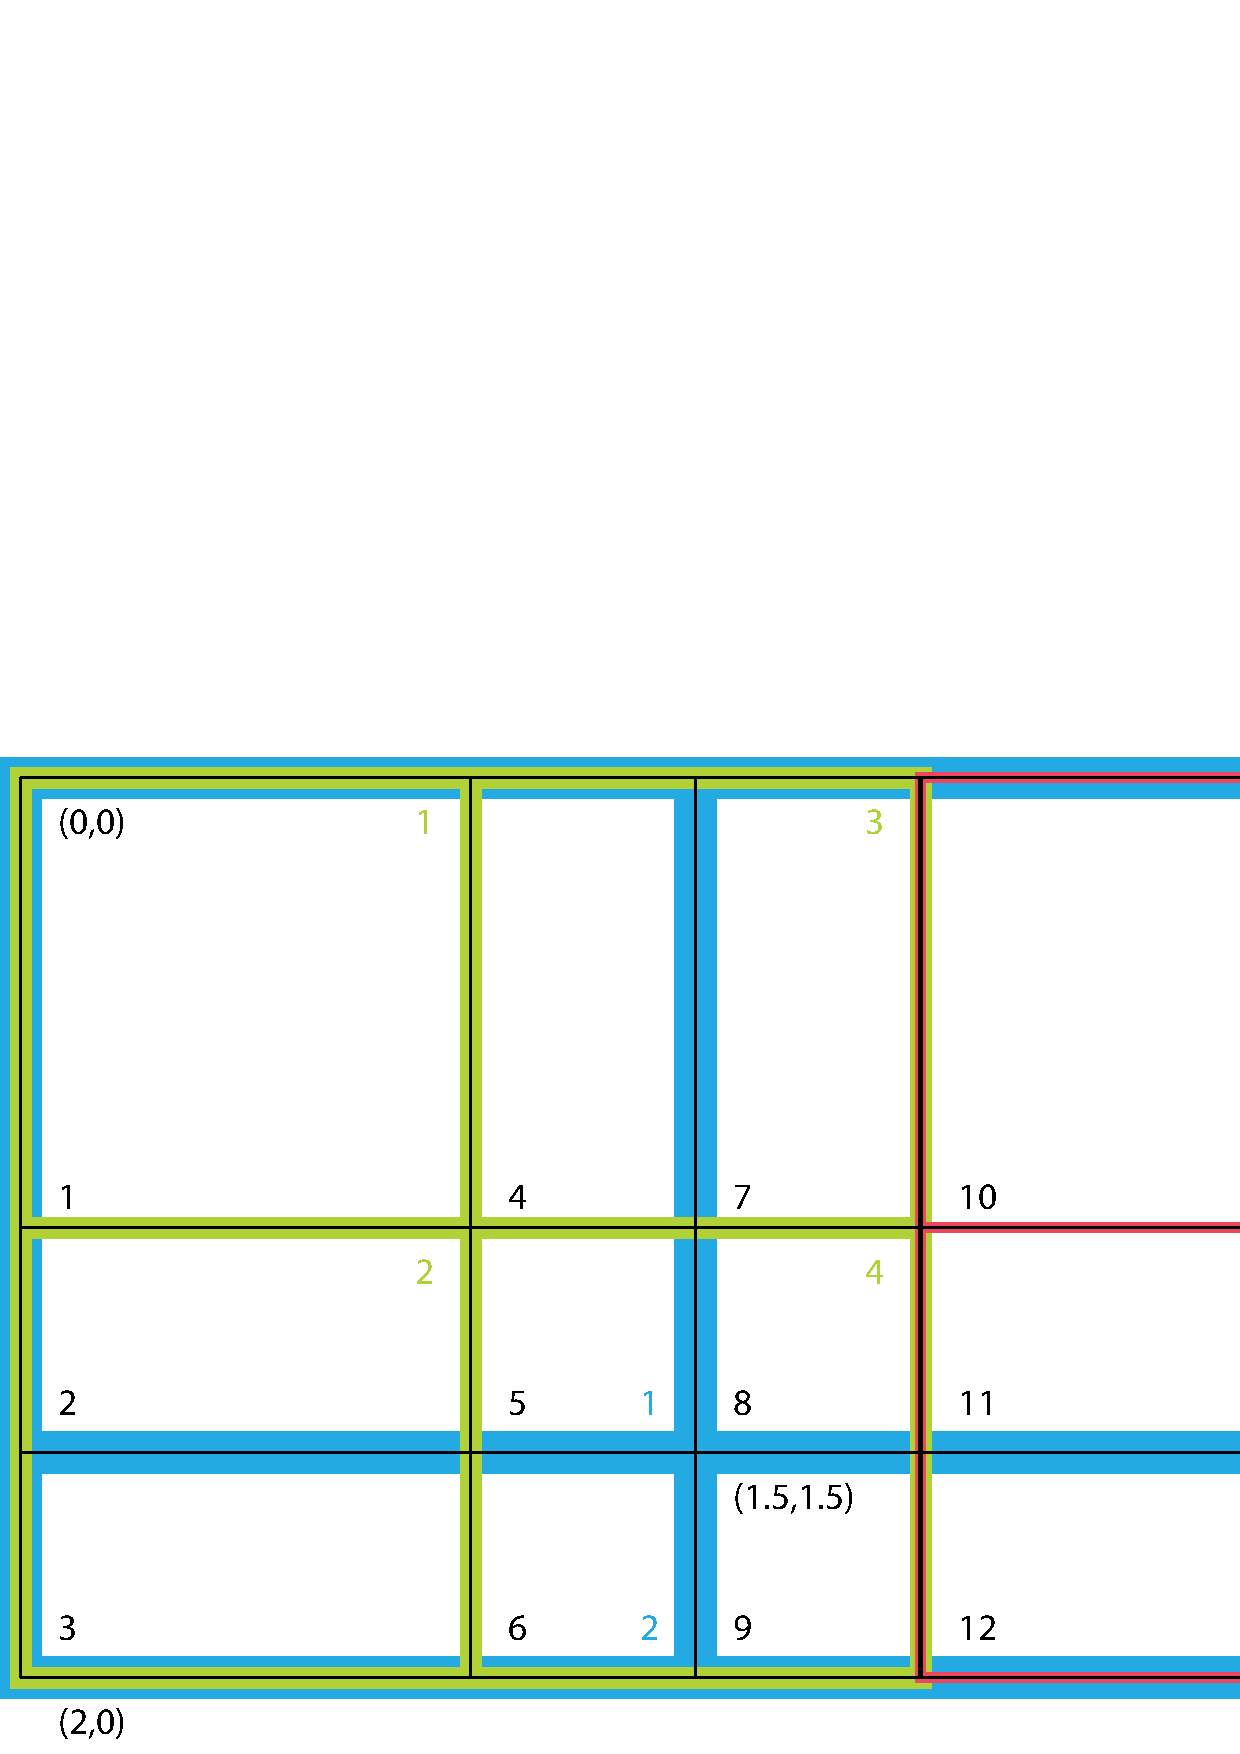
\includegraphics{XGridEx1}}
  \caption{Grid layout for simple XGrid creation example. Overlapping of 3 Grids
  (Green 2x2, Red 2x1, Blue 2x2). Green and red Grids on side A, blue Grid on side
  B, black indicates the resulting XGrid. Color coded sequence indices are shown.
  Physical coordinates are the tuples in parenthesis, e.g. at the four
  corners of rectangular computational domain.}
  \label{fig:xgridsimple}
  \end{figure}
  \end{center}
  
   We start by creating the Grids on both sides and associate coordinates with
   the Grids. For details of Grid creation and coordinate use, please refer to
   Grid class documentation. 
%/////////////////////////////////////////////////////////////

 \begin{verbatim}
    sideA(1) = ESMF_GridCreateNoPeriDim(minIndex=(/1,1/), maxIndex=(/2,2/), &
        coordDep1=(/1/), &
        coordDep2=(/2/), &
        name='source Grid 1 on side A', rc=localrc)
 
\end{verbatim}
 
%/////////////////////////////////////////////////////////////

 \begin{verbatim}
    sideA(2) = ESMF_GridCreateNoPeriDim(minIndex=(/1,1/), maxIndex=(/2,1/), &
        coordDep1=(/1/), &
        coordDep2=(/2/), &
        name='source Grid 2 on side A', rc=localrc)
 
\end{verbatim}
 
%/////////////////////////////////////////////////////////////

 \begin{verbatim}
    do i = 1, 2
        call ESMF_GridAddCoord(sideA(i), staggerloc=ESMF_STAGGERLOC_CENTER, &
            rc=localrc)
 
\end{verbatim}
 
%/////////////////////////////////////////////////////////////

 \begin{verbatim}
    enddo
 
\end{verbatim}
 
%/////////////////////////////////////////////////////////////

   Coordinate for the Grids on sideA, refer to the Grid layout diagram for the
   interpretation of the coordinate values: 
%/////////////////////////////////////////////////////////////

 \begin{verbatim}
    ! SideA first grid
    centroidA1X=(/0.5, 1.5/)
    centroidA1Y=(/0.5, 1.5/)
    call ESMF_GridGetCoord(sideA(1), localDE=0, &
        staggerLoc=ESMF_STAGGERLOC_CENTER, coordDim=1, &
        farrayPtr=coordX, rc=localrc)
 
\end{verbatim}
 
%/////////////////////////////////////////////////////////////

 \begin{verbatim}
    coordX = centroidA1X
    call ESMF_GridGetCoord(sideA(1), localDE=0, &
        staggerLoc=ESMF_STAGGERLOC_CENTER, coordDim=2, &
        farrayPtr=coordY, rc=localrc)
 
\end{verbatim}
 
%/////////////////////////////////////////////////////////////

 \begin{verbatim}
    coordY = centroidA1Y

    ! SideA second grid
    centroidA2X=(/0.5, 1.5/)
    centroidA2Y=(/2.5/)
    call ESMF_GridGetCoord(sideA(2), localDE=0, &
        staggerLoc=ESMF_STAGGERLOC_CENTER, coordDim=1, &
        farrayPtr=coordX, rc=localrc)
 
\end{verbatim}
 
%/////////////////////////////////////////////////////////////

 \begin{verbatim}
    coordX = centroidA2X
    call ESMF_GridGetCoord(sideA(2), localDE=0, &
        staggerLoc=ESMF_STAGGERLOC_CENTER, coordDim=2, &
        farrayPtr=coordY, rc=localrc)
 
\end{verbatim}
 
%/////////////////////////////////////////////////////////////

 \begin{verbatim}
    coordY = centroidA2Y
 
\end{verbatim}
 
%/////////////////////////////////////////////////////////////

   Create the destination grid on side B, only one Grid exists on side B. Also associate
   coordinate with the Grid: 
%/////////////////////////////////////////////////////////////

 \begin{verbatim}
    sideB(1) = ESMF_GridCreateNoPeriDim(minIndex=(/1,1/), maxIndex=(/2,2/), &
        coordDep1=(/1/), coordDep2=(/2/), &
        name='destination Grid on side B', rc=localrc)
 
\end{verbatim}
 
%/////////////////////////////////////////////////////////////

 \begin{verbatim}
    do i = 1, 1
        call ESMF_GridAddCoord(sideB(i), staggerloc=ESMF_STAGGERLOC_CENTER, &
            rc=localrc)
 
\end{verbatim}
 
%/////////////////////////////////////////////////////////////

 \begin{verbatim}
    enddo

    ! SideB grid
    centroidBX=(/0.75, 1.75/)
    centroidBY=(/0.75, 2.25/)
    call ESMF_GridGetCoord(sideB(1), localDE=0, &
        staggerLoc=ESMF_STAGGERLOC_CENTER, coordDim=1, farrayPtr=coordX, &
                rc=localrc)
 
\end{verbatim}
 
%/////////////////////////////////////////////////////////////

 \begin{verbatim}
    coordX = centroidBX
    call ESMF_GridGetCoord(sideB(1), localDE=0, &
        staggerLoc=ESMF_STAGGERLOC_CENTER, coordDim=2, farrayPtr=coordY, &
                rc=localrc)
 
\end{verbatim}
 
%/////////////////////////////////////////////////////////////

 \begin{verbatim}
    coordY = centroidBY
 
\end{verbatim}
 
%/////////////////////////////////////////////////////////////

  
   Set up the mapping indices and weights from A side to the XGrid. For details of
   sequence indices, factorIndexList, and factorList, please see section
   \ref{Array:SparseMatMul} in the reference manual. Please refer to the figure above
   for interpretation of the sequence indices used here.
  
   In order to compute the destination flux on sideB through the XGrid as an mediator,
   we need to set up the factorList (weights) and factorIndexList (indices)
   for sparse matrix multiplication in this formulation:
   dst\_flux = W'*W*src\_flux, where W' is the weight matrix from the XGrid to
   destination; and W is the weight matrix from source to the XGrid. The weight matrix
   is generated using destination area weighted algorithm. Please refer to figure
   \ref {fig:xgridsimple} for details.
   
%/////////////////////////////////////////////////////////////

 \begin{verbatim}
    ! Set up mapping from A1 -> X
    sparseMatA2X(1)%factorIndexList(1,1)=1    ! src seq index (green)
    sparseMatA2X(1)%factorIndexList(1,2)=2    ! src seq index (green)
    sparseMatA2X(1)%factorIndexList(1,3)=2    ! src seq index (green)
    sparseMatA2X(1)%factorIndexList(1,4)=3    ! src seq index (green)
    sparseMatA2X(1)%factorIndexList(1,5)=4    ! src seq index (green)
    sparseMatA2X(1)%factorIndexList(1,6)=4    ! src seq index (green)
    sparseMatA2X(1)%factorIndexList(1,7)=3    ! src seq index (green)
    sparseMatA2X(1)%factorIndexList(1,8)=4    ! src seq index (green)
    sparseMatA2X(1)%factorIndexList(1,9)=4    ! src seq index (green)

    sparseMatA2X(1)%factorIndexList(2,1)=1    ! dst seq index (black)
    sparseMatA2X(1)%factorIndexList(2,2)=2    ! dst seq index (black)
    sparseMatA2X(1)%factorIndexList(2,3)=3    ! dst seq index (black)
    sparseMatA2X(1)%factorIndexList(2,4)=4    ! dst seq index (black)
    sparseMatA2X(1)%factorIndexList(2,5)=5    ! dst seq index (black)
    sparseMatA2X(1)%factorIndexList(2,6)=6    ! dst seq index (black)
    sparseMatA2X(1)%factorIndexList(2,7)=7    ! dst seq index (black)
    sparseMatA2X(1)%factorIndexList(2,8)=8    ! dst seq index (black)
    sparseMatA2X(1)%factorIndexList(2,9)=9    ! dst seq index (black)

    ! Set up mapping from A2 -> X
    sparseMatA2X(2)%factorIndexList(1,1)=1    ! src seq index (red)
    sparseMatA2X(2)%factorIndexList(1,2)=2    ! src seq index (red)
    sparseMatA2X(2)%factorIndexList(1,3)=2    ! src seq index (red)

    sparseMatA2X(2)%factorIndexList(2,1)=10   ! dst seq index (black)
    sparseMatA2X(2)%factorIndexList(2,2)=11   ! dst seq index (black)
    sparseMatA2X(2)%factorIndexList(2,3)=12   ! dst seq index (black)
 
\end{verbatim}
 
%/////////////////////////////////////////////////////////////

   Set up the mapping weights from side A to the XGrid: 
%/////////////////////////////////////////////////////////////

 \begin{verbatim}
    ! Note that the weights are dest area weighted, they are ratio
    ! of areas with destination area as the denominator.
    ! Set up mapping weights from A1 -> X
    sparseMatA2X(1)%factorList(:)=1.

    ! Set up mapping weights from A2 -> X
    sparseMatA2X(2)%factorList(:)=1.
 
\end{verbatim}
 
%/////////////////////////////////////////////////////////////

   Set up the mapping indices and weights from the XGrid to B side: 
%/////////////////////////////////////////////////////////////

 \begin{verbatim}
    ! Set up mapping from X -> B
    sparseMatX2B(1)%factorIndexList(1,1)=1    ! src seq index (black)
    sparseMatX2B(1)%factorIndexList(1,2)=2    ! src seq index (black)
    sparseMatX2B(1)%factorIndexList(1,3)=3    ! src seq index (black)
    sparseMatX2B(1)%factorIndexList(1,4)=4    ! src seq index (black)
    sparseMatX2B(1)%factorIndexList(1,5)=5    ! src seq index (black)
    sparseMatX2B(1)%factorIndexList(1,6)=6    ! src seq index (black)
    sparseMatX2B(1)%factorIndexList(1,7)=7    ! src seq index (black)
    sparseMatX2B(1)%factorIndexList(1,8)=8    ! src seq index (black)
    sparseMatX2B(1)%factorIndexList(1,9)=9    ! src seq index (black)
    sparseMatX2B(1)%factorIndexList(1,10)=10  ! src seq index (black)
    sparseMatX2B(1)%factorIndexList(1,11)=11  ! src seq index (black)
    sparseMatX2B(1)%factorIndexList(1,12)=12  ! src seq index (black)

    sparseMatX2B(1)%factorIndexList(2,1)=1    ! dst seq index (blue)
    sparseMatX2B(1)%factorIndexList(2,2)=1    ! dst seq index (blue)
    sparseMatX2B(1)%factorIndexList(2,3)=2    ! dst seq index (blue)
    sparseMatX2B(1)%factorIndexList(2,4)=1    ! dst seq index (blue)
    sparseMatX2B(1)%factorIndexList(2,5)=1    ! dst seq index (blue)
    sparseMatX2B(1)%factorIndexList(2,6)=2    ! dst seq index (blue)
    sparseMatX2B(1)%factorIndexList(2,7)=3    ! dst seq index (blue)
    sparseMatX2B(1)%factorIndexList(2,8)=3    ! dst seq index (blue)
    sparseMatX2B(1)%factorIndexList(2,9)=4    ! dst seq index (blue)
    sparseMatX2B(1)%factorIndexList(2,10)=3   ! dst seq index (blue)
    sparseMatX2B(1)%factorIndexList(2,11)=3   ! dst seq index (blue)
    sparseMatX2B(1)%factorIndexList(2,12)=4   ! dst seq index (blue)

    ! Set up mapping weights from X -> B
    sparseMatX2B(1)%factorList(1)=4./9.
    sparseMatX2B(1)%factorList(2)=2./9.
    sparseMatX2B(1)%factorList(3)=2./3.
    sparseMatX2B(1)%factorList(4)=2./9.
    sparseMatX2B(1)%factorList(5)=1./9.
    sparseMatX2B(1)%factorList(6)=1./3.
    sparseMatX2B(1)%factorList(7)=2./9.
    sparseMatX2B(1)%factorList(8)=1./9.
    sparseMatX2B(1)%factorList(9)=1./3.
    sparseMatX2B(1)%factorList(10)=4./9.
    sparseMatX2B(1)%factorList(11)=2./9.
    sparseMatX2B(1)%factorList(12)=2./3.
 
\end{verbatim}
 
%/////////////////////////////////////////////////////////////

   Optionally the area can be setup to compute surface area weighted flux integrals: 
%/////////////////////////////////////////////////////////////

 \begin{verbatim}
    ! Set up destination areas to adjust weighted flux
    xgrid_area(1) = 1.
    xgrid_area(2) = 0.5
    xgrid_area(3) = 0.5
    xgrid_area(4) = 0.5
    xgrid_area(5) = 0.25
    xgrid_area(6) = 0.25
    xgrid_area(7) = 0.5
    xgrid_area(8) = 0.25
    xgrid_area(9) = 0.25
    xgrid_area(10) = 1.
    xgrid_area(11) = 0.5
    xgrid_area(12) = 0.5
 
\end{verbatim}
 
%/////////////////////////////////////////////////////////////

   Create an XGrid based on the user supplied regridding parameters: 
%/////////////////////////////////////////////////////////////

 \begin{verbatim}
    xgrid = ESMF_XGridCreateFromSparseMat(sideAGrid=sideA, &
        sideBGrid=sideB, area=xgrid_area, &
        centroid=centroid, sparseMatA2X=sparseMatA2X, &
        sparseMatX2B=sparseMatX2B, rc=localrc)
 
\end{verbatim}
 
%/////////////////////////////////////////////////////////////

   Create an {\tt ESMF\_Field} on the XGrid: 
%/////////////////////////////////////////////////////////////

 \begin{verbatim}
    field = ESMF_FieldCreate(xgrid, typekind=ESMF_TYPEKIND_R8, &
                rc=localrc)
 
\end{verbatim}
 
%/////////////////////////////////////////////////////////////

   Query the Field for its Fortran data pointer and its exclusive bounds: 
%/////////////////////////////////////////////////////////////

 \begin{verbatim}
    call ESMF_FieldGet(field, farrayPtr=xfarrayPtr, &
        exclusiveLBound=xlb, exclusiveUBound=xub, rc=localrc)
 
\end{verbatim}
 
%/////////////////////////////////////////////////////////////

   Setup and initialize src and dst Fields on side A and side B Grids,
   source Fields have different source flux: 
%/////////////////////////////////////////////////////////////

 \begin{verbatim}
    do i = 1, 2
        srcField(i) = ESMF_FieldCreate(sideA(i), &
                typekind=ESMF_TYPEKIND_R8, rc=localrc)
 
\end{verbatim}
 
%/////////////////////////////////////////////////////////////

 \begin{verbatim}
        call ESMF_FieldGet(srcField(i), farrayPtr=farrayPtr, rc=localrc)
 
\end{verbatim}
 
%/////////////////////////////////////////////////////////////

 \begin{verbatim}
        farrayPtr = i
    enddo
    do i = 1, 1
        dstField(i) = ESMF_FieldCreate(sideB(i), &
                typekind=ESMF_TYPEKIND_R8, rc=localrc)
 
\end{verbatim}
 
%/////////////////////////////////////////////////////////////

 \begin{verbatim}
        call ESMF_FieldGet(dstField(i), farrayPtr=farrayPtr, rc=localrc)
 
\end{verbatim}
 
%/////////////////////////////////////////////////////////////

 \begin{verbatim}
        farrayPtr = 0.0
    enddo
 
\end{verbatim}
 
%/////////////////////////////////////////////////////////////

  
   The current implementation requires that Grids used to generate the XGrid
   must not match, i.e. they are different either topologically or geometrically or both.
   In this example, the first source Grid is topologically identical to the destination
   Grid but their geometric coordinates are different. This requirement will be relaxed
   in a future release.
  
   First we compute the regrid routehandles, these routehandles can be used repeatedly
   afterwards. Then we initialize the values in the Fields. Finally we execute the Regrid.
   
%/////////////////////////////////////////////////////////////

 \begin{verbatim}
    ! Compute regrid routehandles. The routehandles can be used
    ! repeatedly afterwards.
    ! From A -> X
    do i = 1, 2
        call ESMF_FieldRegridStore(xgrid, srcField(i), field, &
                routehandle=rh_src2xgrid(i), rc = localrc)
 
\end{verbatim}
 
%/////////////////////////////////////////////////////////////

 \begin{verbatim}
    enddo
    ! from X -> B
    do i = 1, 1
        call ESMF_FieldRegridStore(xgrid, field, dstField(i), &
                routehandle=rh_xgrid2dst(i), rc = localrc)
 
\end{verbatim}
 
%/////////////////////////////////////////////////////////////

 \begin{verbatim}
    enddo

    ! Initialize values in the source Fields on side A
    do i = 1, 2
        call ESMF_FieldGet(srcField(i), farrayPtr=farrayPtr, rc=localrc)
 
\end{verbatim}
 
%/////////////////////////////////////////////////////////////

 \begin{verbatim}
        farrayPtr = i
    enddo
    ! Initialize values in the destination Field on XGrid
    xfarrayPtr = 0.0
    ! Initialize values in the destination Field on Side B
    do i = 1, 1
        call ESMF_FieldGet(dstField(i), farrayPtr=farrayPtr, rc=localrc)
 
\end{verbatim}
 
%/////////////////////////////////////////////////////////////

 \begin{verbatim}
        farrayPtr = 0.0
    enddo
 
\end{verbatim}
 
%/////////////////////////////////////////////////////////////

   First we regrid from the Fields on side A to the Field on the XGrid: 
%/////////////////////////////////////////////////////////////

 \begin{verbatim}
    ! Execute regrid from A -> X
    do i = 1, 2
        call ESMF_FieldRegrid(srcField(i), field, &
            routehandle=rh_src2xgrid(i), &
            zeroregion=ESMF_REGION_SELECT, rc = localrc)
 
\end{verbatim}
 
%/////////////////////////////////////////////////////////////

 \begin{verbatim}
    enddo
 
\end{verbatim}
 
%/////////////////////////////////////////////////////////////

   Next we regrid from the Field on XGrid to the destination Field on side B: 
%/////////////////////////////////////////////////////////////

 \begin{verbatim}
    ! Execute the regrid store
    do i = 1, 1
        call ESMF_FieldRegrid(field, dstField(i), &
            routehandle=rh_xgrid2dst(i), rc = localrc)
 
\end{verbatim}
 
%/////////////////////////////////////////////////////////////

 \begin{verbatim}
    enddo
 
\end{verbatim}
 
%/////////////////////////////////////////////////////////////

   In the above example, we first set up all the required parameters to create an XGrid from user
   supplied input. Then we create Fields on the XGrid and the Grids on either side. Finally
   we use the {\tt ESMF\_FieldRegrid()} interface to perform a flux exchange from the source side
   to the destination side. 
%/////////////////////////////////////////////////////////////

  \subsubsection{Query the XGrid for its internal information}
  \label{sec:xgrid:usage:xgrid_get}
   One can query the XGrid for its internal information: 
%/////////////////////////////////////////////////////////////

 \begin{verbatim}
    call ESMF_XGridGet(xgrid, &
        sideAGridCount=ngridA, &    ! number of Grids on side A
        sideBGridCount=ngridB, &    ! number of Grids on side B
        sideAGrid=l_sideA, &    ! list of Grids on side A
        sideBGrid=l_sideB, &    ! list of Grids on side B
        area=l_area, &      ! list of area of XGrid
        centroid=l_centroid, &  ! list of centroid of XGrid
        distgridA=l_sideAdg, &  ! list of Distgrids on side A
        distgridM = distgrid, & ! balanced distgrid
        sparseMatA2X=l_sparseMatA2X, & !sparse matrix matmul parameters A to X
        sparseMatX2B=l_sparseMatX2B, & !sparse matrix matmul parameters X to B
        rc=localrc)
 
\end{verbatim}
 
%/////////////////////////////////////////////////////////////

 \begin{verbatim}
    call ESMF_XGridGet(xgrid, localDe=0, &
        elementCount=eleCount, &    ! elementCount on the localDE
        exclusiveCount=ec, &        ! exclusive count
        exclusiveLBound=elb, &      ! exclusive lower bound
        exclusiveUBound=eub, &      ! exclusive upper bound
        rc=localrc)
 
\end{verbatim}
 
%/////////////////////////////////////////////////////////////

 \begin{verbatim}
    call ESMF_XGridGet(xgrid, &
        xgridSide=ESMF_XGRIDSIDE_A, & ! side of the XGrid to query
        gridIndex=1, &              ! index of the distgrid
        distgrid=distgrid, &        ! the distgrid returned
        rc=localrc)
 
\end{verbatim}
 
%/////////////////////////////////////////////////////////////

  \subsubsection{Destroying the XGrid and other resources}
  \label{sec:xgrid:usage:xgrid_destroy}
   Clean up the resources by destroying the XGrid and other objects: 
%/////////////////////////////////////////////////////////////

 \begin{verbatim}
    ! After the regridding is successful.
    ! Clean up all the allocated resources:
    call ESMF_FieldDestroy(field, rc=localrc)
 
\end{verbatim}
 
%/////////////////////////////////////////////////////////////

 \begin{verbatim}
    call ESMF_XGridDestroy(xgrid, rc=localrc)
 
\end{verbatim}
 
%/////////////////////////////////////////////////////////////

 \begin{verbatim}
    do i = 1, 2
        call ESMF_FieldDestroy(srcField(i), rc = localrc)
 
\end{verbatim}
 
%/////////////////////////////////////////////////////////////

 \begin{verbatim}
        call ESMF_GridDestroy(sideA(i), rc = localrc)
 
\end{verbatim}
 
%/////////////////////////////////////////////////////////////

 \begin{verbatim}
    enddo

    do i = 1, 1
        call ESMF_FieldDestroy(dstField(i), rc = localrc)
 
\end{verbatim}
 
%/////////////////////////////////////////////////////////////

 \begin{verbatim}
        call ESMF_GridDestroy(sideB(i), rc = localrc)
 
\end{verbatim}
 
%/////////////////////////////////////////////////////////////

 \begin{verbatim}
    enddo

    deallocate(sparseMatA2X(1)%factorIndexList, sparseMatA2X(1)%factorList)
    deallocate(sparseMatA2X(2)%factorIndexList, sparseMatA2X(2)%factorList)
    deallocate(sparseMatX2B(1)%factorIndexList, sparseMatX2B(1)%factorList)
 
\end{verbatim}

%...............................................................
\setlength{\parskip}{\oldparskip}
\setlength{\parindent}{\oldparindent}
\setlength{\baselineskip}{\oldbaselineskip}

%#elif defined(1)
%\input{../Infrastructure/XGrid/doc/XGrid_usage}
%%                **** IMPORTANT NOTICE *****
% This LaTeX file has been automatically produced by ProTeX v. 1.1
% Any changes made to this file will likely be lost next time
% this file is regenerated from its source. Send questions 
% to Arlindo da Silva, dasilva@gsfc.nasa.gov
 
\setlength{\oldparskip}{\parskip}
\setlength{\parskip}{1.5ex}
\setlength{\oldparindent}{\parindent}
\setlength{\parindent}{0pt}
\setlength{\oldbaselineskip}{\baselineskip}
\setlength{\baselineskip}{11pt}
 
%--------------------- SHORT-HAND MACROS ----------------------
\def\bv{\begin{verbatim}}
\def\ev{\end{verbatim}}
\def\be{\begin{equation}}
\def\ee{\end{equation}}
\def\bea{\begin{eqnarray}}
\def\eea{\end{eqnarray}}
\def\bi{\begin{itemize}}
\def\ei{\end{itemize}}
\def\bn{\begin{enumerate}}
\def\en{\end{enumerate}}
\def\bd{\begin{description}}
\def\ed{\end{description}}
\def\({\left (}
\def\){\right )}
\def\[{\left [}
\def\]{\right ]}
\def\<{\left  \langle}
\def\>{\right \rangle}
\def\cI{{\cal I}}
\def\diag{\mathop{\rm diag}}
\def\tr{\mathop{\rm tr}}
%-------------------------------------------------------------

\markboth{Left}{Source File: ESMF\_XGridEx.F90,  Date: Tue May  5 20:59:57 MDT 2020
}

 
%/////////////////////////////////////////////////////////////

  \subsubsection{Create an XGrid from Grids then use it for regridding}
  \label{sec:xgrid:usage:xgrid_create}
  
   An {\tt ESMF\_XGrid} object can be created from Grids on either side
   of the exchange grid. Internally the
   weight matrices and index mapping are computed and stored in the XGrid, along
   with other necessary information for flux exchange calculation between
   any pair of model components used for the XGrid creation.
  
   In this example, we create an XGrid from overlapping Grids on
   either side of the XGrid. Then we perform a flux exchange from one side
   to the other side of the XGrid.
  
   We start by creating the Grids on both sides and associate coordinates with
   the Grids on the corner stagger. The Grids use global indexing and padding
   for coordinates on the corner stagger.
  
   For details of Grid creation and coordinate use,
   please refer to Grid class documentation: \ref{example:2DRegUniGrid}. 
%/////////////////////////////////////////////////////////////

 \begin{verbatim}
    ! First Grid on side A
    sideA(1) = ESMF_GridCreateNoPeriDim(maxIndex=(/20, 20/), &
      indexflag=ESMF_INDEX_GLOBAL, &
      gridEdgeLWidth=(/0,0/), gridEdgeUWidth=(/1,1/), &
      name='source Grid 1 on side A', rc=localrc)
 
\end{verbatim}
 
%/////////////////////////////////////////////////////////////

 \begin{verbatim}
    ! Second Grid on side A
    sideA(2) = ESMF_GridCreateNoPeriDim(maxIndex=(/20, 10/), &
      indexflag=ESMF_INDEX_GLOBAL, &
      gridEdgeLWidth=(/0,0/), gridEdgeUWidth=(/1,1/), &
      name='source Grid 2 on side A', rc=localrc)
 
\end{verbatim}
 
%/////////////////////////////////////////////////////////////

 \begin{verbatim}
    ! Allocate coordinates for Grid corner stagger
    do i = 1, 2
      call ESMF_GridAddCoord(sideA(i), staggerloc=ESMF_STAGGERLOC_CORNER, &
          rc=localrc)
 
\end{verbatim}
 
%/////////////////////////////////////////////////////////////

 \begin{verbatim}
    enddo
 
\end{verbatim}
 
%/////////////////////////////////////////////////////////////

   Assign coordinate for the Grids on sideA at corner stagger. 
%/////////////////////////////////////////////////////////////

 \begin{verbatim}
    ! SideA first grid spans (0-20, 0-20) with 1.0x1.0 degree resolution
    ! X corner
    call ESMF_GridGetCoord(sideA(1), localDE=0, &
        staggerLoc=ESMF_STAGGERLOC_CORNER, coordDim=1, &
        farrayPtr=coordX, rc=localrc)
 
\end{verbatim}
 
%/////////////////////////////////////////////////////////////

 \begin{verbatim}
    ! Y corner
    call ESMF_GridGetCoord(sideA(1), localDE=0, &
        staggerLoc=ESMF_STAGGERLOC_CORNER, coordDim=2, &
        farrayPtr=coordY, rc=localrc)
 
\end{verbatim}
 
%/////////////////////////////////////////////////////////////

 \begin{verbatim}
    do i = lbound(coordX,1), ubound(coordX,1)
      do j = lbound(coordX, 2), ubound(coordX, 2)
        coordX(i,j) = (i-1)*1.0
        coordY(i,j) = (j-1)*1.0
      enddo
    enddo
 
\end{verbatim}
 
%/////////////////////////////////////////////////////////////

 \begin{verbatim}
    ! SideA second grid spans (14.3-24.3, 14.2-24.2) with 0.5x1.0 degree
    ! resolution X corner
    call ESMF_GridGetCoord(sideA(2), localDE=0, &
        staggerLoc=ESMF_STAGGERLOC_CORNER, coordDim=1, &
        farrayPtr=coordX, rc=localrc)
 
\end{verbatim}
 
%/////////////////////////////////////////////////////////////

 \begin{verbatim}
    ! Y corner
    call ESMF_GridGetCoord(sideA(2), localDE=0, &
        staggerLoc=ESMF_STAGGERLOC_CORNER, coordDim=2, &
        farrayPtr=coordY, rc=localrc)
 
\end{verbatim}
 
%/////////////////////////////////////////////////////////////

 \begin{verbatim}
    do i = lbound(coordX,1), ubound(coordX,1)
      do j = lbound(coordX, 2), ubound(coordX, 2)
        coordX(i,j) = 14.3+(i-1)*0.5
        coordY(i,j) = 14.2+(j-1)*1.0
      enddo
    enddo
 
\end{verbatim}
 
%/////////////////////////////////////////////////////////////

   Create the destination grid on side B, only one Grid exists on side B. Also associate
   coordinate with the Grid: 
%/////////////////////////////////////////////////////////////

 \begin{verbatim}
    sideB(1) = ESMF_GridCreateNoPeriDim(maxIndex=(/30, 30/), &
      indexflag=ESMF_INDEX_GLOBAL, &
      gridEdgeLWidth=(/0,0/), gridEdgeUWidth=(/1,1/), &
      name='source Grid 1 on side B', rc=localrc)
 
\end{verbatim}
 
%/////////////////////////////////////////////////////////////

 \begin{verbatim}
    do i = 1, 1
      call ESMF_GridAddCoord(sideB(i), staggerloc=ESMF_STAGGERLOC_CORNER, &
          rc=localrc)
 
\end{verbatim}
 
%/////////////////////////////////////////////////////////////

 \begin{verbatim}
    enddo
 
\end{verbatim}
 
%/////////////////////////////////////////////////////////////

 \begin{verbatim}
    ! SideB grid spans (0-30, 0-30) with 1.0x1.0 degree resolution
    ! X corner
    call ESMF_GridGetCoord(sideB(1), localDE=0, &
        staggerLoc=ESMF_STAGGERLOC_CORNER, coordDim=1, &
        farrayPtr=coordX, rc=localrc)
 
\end{verbatim}
 
%/////////////////////////////////////////////////////////////

 \begin{verbatim}
    ! Y corner
    call ESMF_GridGetCoord(sideB(1), localDE=0, &
        staggerLoc=ESMF_STAGGERLOC_CORNER, coordDim=2, &
        farrayPtr=coordY, rc=localrc)
 
\end{verbatim}
 
%/////////////////////////////////////////////////////////////

 \begin{verbatim}
    do i = lbound(coordX,1), ubound(coordX,1)
      do j = lbound(coordX, 2), ubound(coordX, 2)
        coordX(i,j) = (i-1)*1.0
        coordY(i,j) = (j-1)*1.0
      enddo
    enddo
 
\end{verbatim}
 
%/////////////////////////////////////////////////////////////

   Create an {\tt ESMF\_XGrid} object from the two lists of Grids on side A and B.
   In this example both Grids on side A overlaps with the Grid on side B. It's an error to have a Grid
   on either side that is spatially disjoint with the XGrid. Neither of the Grid on side A is
   identical to the Grid on side B. Calling the {\tt ESMF\_XGridCreate()} method is straightforward: 
%/////////////////////////////////////////////////////////////

 \begin{verbatim}
    xgrid = ESMF_XGridCreate(sideAGrid=sideA, sideBGrid=sideB, rc=localrc)
 
\end{verbatim}
 
%/////////////////////////////////////////////////////////////

   Create an {\tt ESMF\_Field} on the XGrid: 
%/////////////////////////////////////////////////////////////

 \begin{verbatim}
    field = ESMF_FieldCreate(xgrid, typekind=ESMF_TYPEKIND_R8, &
                rc=localrc)
 
\end{verbatim}
 
%/////////////////////////////////////////////////////////////

   Query the Field for its Fortran data pointer and its exclusive bounds: 
%/////////////////////////////////////////////////////////////

 \begin{verbatim}
    call ESMF_FieldGet(field, farrayPtr=xfarrayPtr, &
        exclusiveLBound=xlb, exclusiveUBound=xub, rc=localrc)
 
\end{verbatim}
 
%/////////////////////////////////////////////////////////////

   Create src and dst Fields on side A and side B Grids. 
%/////////////////////////////////////////////////////////////

 \begin{verbatim}
    do i = 1, 2
        srcField(i) = ESMF_FieldCreate(sideA(i), &
                typekind=ESMF_TYPEKIND_R8, rc=localrc)
 
\end{verbatim}
 
%/////////////////////////////////////////////////////////////

 \begin{verbatim}
    enddo
    do i = 1, 1
        dstField(i) = ESMF_FieldCreate(sideB(i), &
                typekind=ESMF_TYPEKIND_R8, rc=localrc)
 
\end{verbatim}
 
%/////////////////////////////////////////////////////////////

 \begin{verbatim}
    enddo
 
\end{verbatim}
 
%/////////////////////////////////////////////////////////////

  
   The current implementation requires that Grids used to generate the XGrid
   must not match, i.e. they are different either topologically or geometrically or both.
   In this example, the first source Grid is topologically identical to the destination
   Grid but their geometric coordinates are different.
  
   First we compute the regrid routehandles, these routehandles can be used repeatedly
   afterwards. Then we initialize the values in the Fields. Finally we execute the Regrid.
   
%/////////////////////////////////////////////////////////////

 \begin{verbatim}
    ! Compute regrid routehandles. The routehandles can be used
    ! repeatedly afterwards.
    ! From A -> X
    do i = 1, 2
      call ESMF_FieldRegridStore(xgrid, srcField(i), field, &
        routehandle=rh_src2xgrid(i), rc = localrc)
 
\end{verbatim}
 
%/////////////////////////////////////////////////////////////

 \begin{verbatim}
    enddo
    ! from X -> B, retrieve the destination fraction Fields.
    do i = 1, 1
      call ESMF_FieldRegridStore(xgrid, field, dstField(i), &
        dstFracField=dstFrac, dstMergeFracField=dstFrac2, &
        routehandle=rh_xgrid2dst(i), rc = localrc)
 
\end{verbatim}
 
%/////////////////////////////////////////////////////////////

 \begin{verbatim}
    enddo

    ! Initialize values in the source Fields on side A
    do i = 1, 2
      call ESMF_FieldGet(srcField(i), farrayPtr=farrayPtr, rc=localrc)
 
\end{verbatim}
 
%/////////////////////////////////////////////////////////////

 \begin{verbatim}
      farrayPtr = i
    enddo
    ! Initialize values in the destination Field on XGrid
    xfarrayPtr = 0.0
    ! Initialize values in the destination Field on Side B
    do i = 1, 1
      call ESMF_FieldGet(dstField(i), farrayPtr=farrayPtr, rc=localrc)
 
\end{verbatim}
 
%/////////////////////////////////////////////////////////////

 \begin{verbatim}
      farrayPtr = 0.0
    enddo
 
\end{verbatim}
 
%/////////////////////////////////////////////////////////////

   First we regrid from the Fields on side A to the Field on the XGrid: 
%/////////////////////////////////////////////////////////////

 \begin{verbatim}
    ! Execute regrid from A -> X
    do i = 1, 2
      call ESMF_FieldRegrid(srcField(i), field, &
        routehandle=rh_src2xgrid(i), &
        zeroregion=ESMF_REGION_SELECT, rc = localrc)
 
\end{verbatim}
 
%/////////////////////////////////////////////////////////////

 \begin{verbatim}
    enddo
 
\end{verbatim}
 
%/////////////////////////////////////////////////////////////

   Next we regrid from the Field on XGrid to the destination Field on side B: 
%/////////////////////////////////////////////////////////////

 \begin{verbatim}
    ! Execute the regrid store
    do i = 1, 1
      call ESMF_FieldRegrid(field, dstField(i), &
        routehandle=rh_xgrid2dst(i), &
        rc = localrc)
 
\end{verbatim}
 
%/////////////////////////////////////////////////////////////

 \begin{verbatim}
    enddo
 
\end{verbatim}
 
%/////////////////////////////////////////////////////////////

   After the regridding calls, the routehandle can be released by calling the
   {\tt ESMF\_FieldRegridRelease()} method. 
%/////////////////////////////////////////////////////////////

 \begin{verbatim}
    do i = 1, 2
      call ESMF_FieldRegridRelease(routehandle=rh_src2xgrid(i), rc=localrc)
 
\end{verbatim}
 
%/////////////////////////////////////////////////////////////

 \begin{verbatim}
    enddo
    call ESMF_FieldRegridRelease(routehandle=rh_xgrid2dst(1), rc=localrc)
 
\end{verbatim}
 
 
%/////////////////////////////////////////////////////////////

   In the above example, we first set up all the required parameters to create an XGrid from user
   supplied input. Then we create Fields on the XGrid and the Grids on either side. Finally
   we use the {\tt ESMF\_FieldRegrid()} interface to perform a flux exchange from the source side
   to the destination side. 
%/////////////////////////////////////////////////////////////

  \subsubsection{Using XGrid in Earth System modeling}
  \label{sec:xgrid:usage:xgrid_create_masking}
  
   A typical application in Earth System Modeling is to calculate flux exchange
   through the planetary boundary layer that can be represented by {\tt ESMF\_XGrid}.
   Atmosphere is above the planetary boundary layer while land and ocean are below the boundary layer.
   To create an XGrid, the land and ocean Grids that are usually different in resolution
   need to be merged first to create a super Mesh. This merging process is enabled through the support
   of masking.
  
   The global land and ocean Grids need to be created with masking enabled.
   In practice, each Grid cell has an integer masking value attached to it. For examples using masking in
   {\tt ESMF\_Grid} please refer to section \ref{sec:usage:items}.
  
   When calling the {\tt ESMF\_XGridCreate()} method, user can supply the optional arguments
   sideAMaskValues and sideBMaskValues.
   These arguments are one dimensional Fortran integer arrays. If any of the sideAMaskValues entry
   matches the masking value used in sideA Grid, the sideA Grid cell is masked out, vice versa for sideB.
   Thus by specifying different regions of a land and ocean Grids to be masked out, the two global Grids
   can be merged into a new global Mesh covering the entire Earth.
  
   The following call shows how to use the {\tt ESMF\_XGridCreate()} method with the optional
   arguments sideAMaskValues and sideBMaskValues.
   
%/////////////////////////////////////////////////////////////

 \begin{verbatim}
    xgrid = ESMF_XGridCreate(sideAGrid=sideA, sideBGrid=sideB, &
      sideAMaskValues=(/2/), sideBMaskValues=(/3,4/), rc=localrc)
 
\end{verbatim}

%...............................................................
\setlength{\parskip}{\oldparskip}
\setlength{\parindent}{\oldparindent}
\setlength{\baselineskip}{\oldbaselineskip}

%%                **** IMPORTANT NOTICE *****
% This LaTeX file has been automatically produced by ProTeX v. 1.1
% Any changes made to this file will likely be lost next time
% this file is regenerated from its source. Send questions 
% to Arlindo da Silva, dasilva@gsfc.nasa.gov
 
\setlength{\oldparskip}{\parskip}
\setlength{\parskip}{1.5ex}
\setlength{\oldparindent}{\parindent}
\setlength{\parindent}{0pt}
\setlength{\oldbaselineskip}{\baselineskip}
\setlength{\baselineskip}{11pt}
 
%--------------------- SHORT-HAND MACROS ----------------------
\def\bv{\begin{verbatim}}
\def\ev{\end{verbatim}}
\def\be{\begin{equation}}
\def\ee{\end{equation}}
\def\bea{\begin{eqnarray}}
\def\eea{\end{eqnarray}}
\def\bi{\begin{itemize}}
\def\ei{\end{itemize}}
\def\bn{\begin{enumerate}}
\def\en{\end{enumerate}}
\def\bd{\begin{description}}
\def\ed{\end{description}}
\def\({\left (}
\def\){\right )}
\def\[{\left [}
\def\]{\right ]}
\def\<{\left  \langle}
\def\>{\right \rangle}
\def\cI{{\cal I}}
\def\diag{\mathop{\rm diag}}
\def\tr{\mathop{\rm tr}}
%-------------------------------------------------------------

\markboth{Left}{Source File: ESMF\_XGridSparseMatEx.F90,  Date: Tue May  5 20:59:57 MDT 2020
}

 
%/////////////////////////////////////////////////////////////

  \subsubsection{Create an XGrid from user input data then use it for regridding}
  \label{sec:xgrid:usage:xgrid_createfromsparsemat}
  
   Alternatively, XGrid can be created from Grids on either side,
   area and centroid information of XGrid cells, sparse matrix matmul information.
   The functionalities provided by the
   XGrid object is constrained by the user supplied input during its creation time.
  
   In this example, we will set up a simple XGrid from overlapping Grids on
   either side of the XGrid. Then we perform a flux exchange from one side
   to the other side of the XGrid. The Grids are laid out in the following figure:
  \begin{center}
  \begin{figure}
  \center
  \scalebox{0.6}{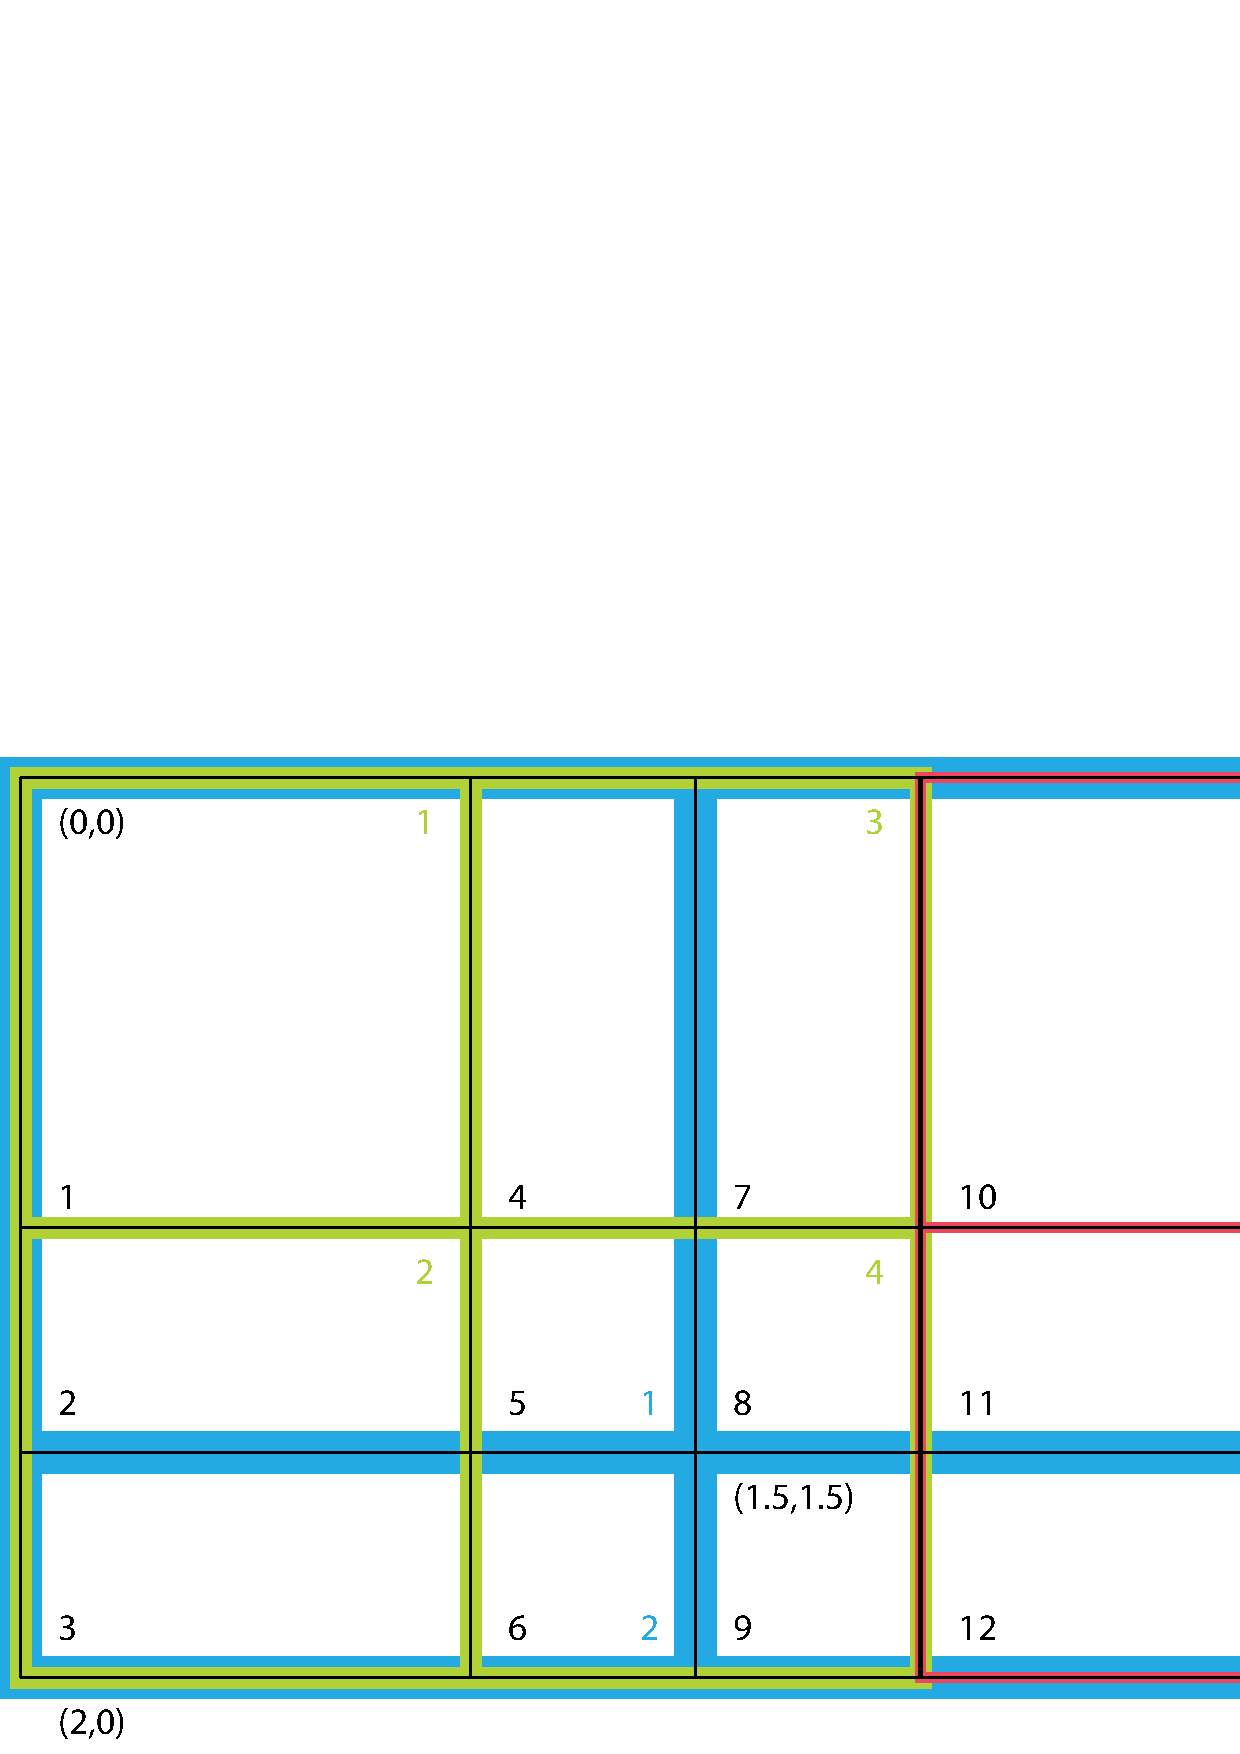
\includegraphics{XGridEx1}}
  \caption{Grid layout for simple XGrid creation example. Overlapping of 3 Grids
  (Green 2x2, Red 2x1, Blue 2x2). Green and red Grids on side A, blue Grid on side
  B, black indicates the resulting XGrid. Color coded sequence indices are shown.
  Physical coordinates are the tuples in parenthesis, e.g. at the four
  corners of rectangular computational domain.}
  \label{fig:xgridsimple}
  \end{figure}
  \end{center}
  
   We start by creating the Grids on both sides and associate coordinates with
   the Grids. For details of Grid creation and coordinate use, please refer to
   Grid class documentation. 
%/////////////////////////////////////////////////////////////

 \begin{verbatim}
    sideA(1) = ESMF_GridCreateNoPeriDim(minIndex=(/1,1/), maxIndex=(/2,2/), &
        coordDep1=(/1/), &
        coordDep2=(/2/), &
        name='source Grid 1 on side A', rc=localrc)
 
\end{verbatim}
 
%/////////////////////////////////////////////////////////////

 \begin{verbatim}
    sideA(2) = ESMF_GridCreateNoPeriDim(minIndex=(/1,1/), maxIndex=(/2,1/), &
        coordDep1=(/1/), &
        coordDep2=(/2/), &
        name='source Grid 2 on side A', rc=localrc)
 
\end{verbatim}
 
%/////////////////////////////////////////////////////////////

 \begin{verbatim}
    do i = 1, 2
        call ESMF_GridAddCoord(sideA(i), staggerloc=ESMF_STAGGERLOC_CENTER, &
            rc=localrc)
 
\end{verbatim}
 
%/////////////////////////////////////////////////////////////

 \begin{verbatim}
    enddo
 
\end{verbatim}
 
%/////////////////////////////////////////////////////////////

   Coordinate for the Grids on sideA, refer to the Grid layout diagram for the
   interpretation of the coordinate values: 
%/////////////////////////////////////////////////////////////

 \begin{verbatim}
    ! SideA first grid
    centroidA1X=(/0.5, 1.5/)
    centroidA1Y=(/0.5, 1.5/)
    call ESMF_GridGetCoord(sideA(1), localDE=0, &
        staggerLoc=ESMF_STAGGERLOC_CENTER, coordDim=1, &
        farrayPtr=coordX, rc=localrc)
 
\end{verbatim}
 
%/////////////////////////////////////////////////////////////

 \begin{verbatim}
    coordX = centroidA1X
    call ESMF_GridGetCoord(sideA(1), localDE=0, &
        staggerLoc=ESMF_STAGGERLOC_CENTER, coordDim=2, &
        farrayPtr=coordY, rc=localrc)
 
\end{verbatim}
 
%/////////////////////////////////////////////////////////////

 \begin{verbatim}
    coordY = centroidA1Y

    ! SideA second grid
    centroidA2X=(/0.5, 1.5/)
    centroidA2Y=(/2.5/)
    call ESMF_GridGetCoord(sideA(2), localDE=0, &
        staggerLoc=ESMF_STAGGERLOC_CENTER, coordDim=1, &
        farrayPtr=coordX, rc=localrc)
 
\end{verbatim}
 
%/////////////////////////////////////////////////////////////

 \begin{verbatim}
    coordX = centroidA2X
    call ESMF_GridGetCoord(sideA(2), localDE=0, &
        staggerLoc=ESMF_STAGGERLOC_CENTER, coordDim=2, &
        farrayPtr=coordY, rc=localrc)
 
\end{verbatim}
 
%/////////////////////////////////////////////////////////////

 \begin{verbatim}
    coordY = centroidA2Y
 
\end{verbatim}
 
%/////////////////////////////////////////////////////////////

   Create the destination grid on side B, only one Grid exists on side B. Also associate
   coordinate with the Grid: 
%/////////////////////////////////////////////////////////////

 \begin{verbatim}
    sideB(1) = ESMF_GridCreateNoPeriDim(minIndex=(/1,1/), maxIndex=(/2,2/), &
        coordDep1=(/1/), coordDep2=(/2/), &
        name='destination Grid on side B', rc=localrc)
 
\end{verbatim}
 
%/////////////////////////////////////////////////////////////

 \begin{verbatim}
    do i = 1, 1
        call ESMF_GridAddCoord(sideB(i), staggerloc=ESMF_STAGGERLOC_CENTER, &
            rc=localrc)
 
\end{verbatim}
 
%/////////////////////////////////////////////////////////////

 \begin{verbatim}
    enddo

    ! SideB grid
    centroidBX=(/0.75, 1.75/)
    centroidBY=(/0.75, 2.25/)
    call ESMF_GridGetCoord(sideB(1), localDE=0, &
        staggerLoc=ESMF_STAGGERLOC_CENTER, coordDim=1, farrayPtr=coordX, &
                rc=localrc)
 
\end{verbatim}
 
%/////////////////////////////////////////////////////////////

 \begin{verbatim}
    coordX = centroidBX
    call ESMF_GridGetCoord(sideB(1), localDE=0, &
        staggerLoc=ESMF_STAGGERLOC_CENTER, coordDim=2, farrayPtr=coordY, &
                rc=localrc)
 
\end{verbatim}
 
%/////////////////////////////////////////////////////////////

 \begin{verbatim}
    coordY = centroidBY
 
\end{verbatim}
 
%/////////////////////////////////////////////////////////////

  
   Set up the mapping indices and weights from A side to the XGrid. For details of
   sequence indices, factorIndexList, and factorList, please see section
   \ref{Array:SparseMatMul} in the reference manual. Please refer to the figure above
   for interpretation of the sequence indices used here.
  
   In order to compute the destination flux on sideB through the XGrid as an mediator,
   we need to set up the factorList (weights) and factorIndexList (indices)
   for sparse matrix multiplication in this formulation:
   dst\_flux = W'*W*src\_flux, where W' is the weight matrix from the XGrid to
   destination; and W is the weight matrix from source to the XGrid. The weight matrix
   is generated using destination area weighted algorithm. Please refer to figure
   \ref {fig:xgridsimple} for details.
   
%/////////////////////////////////////////////////////////////

 \begin{verbatim}
    ! Set up mapping from A1 -> X
    sparseMatA2X(1)%factorIndexList(1,1)=1    ! src seq index (green)
    sparseMatA2X(1)%factorIndexList(1,2)=2    ! src seq index (green)
    sparseMatA2X(1)%factorIndexList(1,3)=2    ! src seq index (green)
    sparseMatA2X(1)%factorIndexList(1,4)=3    ! src seq index (green)
    sparseMatA2X(1)%factorIndexList(1,5)=4    ! src seq index (green)
    sparseMatA2X(1)%factorIndexList(1,6)=4    ! src seq index (green)
    sparseMatA2X(1)%factorIndexList(1,7)=3    ! src seq index (green)
    sparseMatA2X(1)%factorIndexList(1,8)=4    ! src seq index (green)
    sparseMatA2X(1)%factorIndexList(1,9)=4    ! src seq index (green)

    sparseMatA2X(1)%factorIndexList(2,1)=1    ! dst seq index (black)
    sparseMatA2X(1)%factorIndexList(2,2)=2    ! dst seq index (black)
    sparseMatA2X(1)%factorIndexList(2,3)=3    ! dst seq index (black)
    sparseMatA2X(1)%factorIndexList(2,4)=4    ! dst seq index (black)
    sparseMatA2X(1)%factorIndexList(2,5)=5    ! dst seq index (black)
    sparseMatA2X(1)%factorIndexList(2,6)=6    ! dst seq index (black)
    sparseMatA2X(1)%factorIndexList(2,7)=7    ! dst seq index (black)
    sparseMatA2X(1)%factorIndexList(2,8)=8    ! dst seq index (black)
    sparseMatA2X(1)%factorIndexList(2,9)=9    ! dst seq index (black)

    ! Set up mapping from A2 -> X
    sparseMatA2X(2)%factorIndexList(1,1)=1    ! src seq index (red)
    sparseMatA2X(2)%factorIndexList(1,2)=2    ! src seq index (red)
    sparseMatA2X(2)%factorIndexList(1,3)=2    ! src seq index (red)

    sparseMatA2X(2)%factorIndexList(2,1)=10   ! dst seq index (black)
    sparseMatA2X(2)%factorIndexList(2,2)=11   ! dst seq index (black)
    sparseMatA2X(2)%factorIndexList(2,3)=12   ! dst seq index (black)
 
\end{verbatim}
 
%/////////////////////////////////////////////////////////////

   Set up the mapping weights from side A to the XGrid: 
%/////////////////////////////////////////////////////////////

 \begin{verbatim}
    ! Note that the weights are dest area weighted, they are ratio
    ! of areas with destination area as the denominator.
    ! Set up mapping weights from A1 -> X
    sparseMatA2X(1)%factorList(:)=1.

    ! Set up mapping weights from A2 -> X
    sparseMatA2X(2)%factorList(:)=1.
 
\end{verbatim}
 
%/////////////////////////////////////////////////////////////

   Set up the mapping indices and weights from the XGrid to B side: 
%/////////////////////////////////////////////////////////////

 \begin{verbatim}
    ! Set up mapping from X -> B
    sparseMatX2B(1)%factorIndexList(1,1)=1    ! src seq index (black)
    sparseMatX2B(1)%factorIndexList(1,2)=2    ! src seq index (black)
    sparseMatX2B(1)%factorIndexList(1,3)=3    ! src seq index (black)
    sparseMatX2B(1)%factorIndexList(1,4)=4    ! src seq index (black)
    sparseMatX2B(1)%factorIndexList(1,5)=5    ! src seq index (black)
    sparseMatX2B(1)%factorIndexList(1,6)=6    ! src seq index (black)
    sparseMatX2B(1)%factorIndexList(1,7)=7    ! src seq index (black)
    sparseMatX2B(1)%factorIndexList(1,8)=8    ! src seq index (black)
    sparseMatX2B(1)%factorIndexList(1,9)=9    ! src seq index (black)
    sparseMatX2B(1)%factorIndexList(1,10)=10  ! src seq index (black)
    sparseMatX2B(1)%factorIndexList(1,11)=11  ! src seq index (black)
    sparseMatX2B(1)%factorIndexList(1,12)=12  ! src seq index (black)

    sparseMatX2B(1)%factorIndexList(2,1)=1    ! dst seq index (blue)
    sparseMatX2B(1)%factorIndexList(2,2)=1    ! dst seq index (blue)
    sparseMatX2B(1)%factorIndexList(2,3)=2    ! dst seq index (blue)
    sparseMatX2B(1)%factorIndexList(2,4)=1    ! dst seq index (blue)
    sparseMatX2B(1)%factorIndexList(2,5)=1    ! dst seq index (blue)
    sparseMatX2B(1)%factorIndexList(2,6)=2    ! dst seq index (blue)
    sparseMatX2B(1)%factorIndexList(2,7)=3    ! dst seq index (blue)
    sparseMatX2B(1)%factorIndexList(2,8)=3    ! dst seq index (blue)
    sparseMatX2B(1)%factorIndexList(2,9)=4    ! dst seq index (blue)
    sparseMatX2B(1)%factorIndexList(2,10)=3   ! dst seq index (blue)
    sparseMatX2B(1)%factorIndexList(2,11)=3   ! dst seq index (blue)
    sparseMatX2B(1)%factorIndexList(2,12)=4   ! dst seq index (blue)

    ! Set up mapping weights from X -> B
    sparseMatX2B(1)%factorList(1)=4./9.
    sparseMatX2B(1)%factorList(2)=2./9.
    sparseMatX2B(1)%factorList(3)=2./3.
    sparseMatX2B(1)%factorList(4)=2./9.
    sparseMatX2B(1)%factorList(5)=1./9.
    sparseMatX2B(1)%factorList(6)=1./3.
    sparseMatX2B(1)%factorList(7)=2./9.
    sparseMatX2B(1)%factorList(8)=1./9.
    sparseMatX2B(1)%factorList(9)=1./3.
    sparseMatX2B(1)%factorList(10)=4./9.
    sparseMatX2B(1)%factorList(11)=2./9.
    sparseMatX2B(1)%factorList(12)=2./3.
 
\end{verbatim}
 
%/////////////////////////////////////////////////////////////

   Optionally the area can be setup to compute surface area weighted flux integrals: 
%/////////////////////////////////////////////////////////////

 \begin{verbatim}
    ! Set up destination areas to adjust weighted flux
    xgrid_area(1) = 1.
    xgrid_area(2) = 0.5
    xgrid_area(3) = 0.5
    xgrid_area(4) = 0.5
    xgrid_area(5) = 0.25
    xgrid_area(6) = 0.25
    xgrid_area(7) = 0.5
    xgrid_area(8) = 0.25
    xgrid_area(9) = 0.25
    xgrid_area(10) = 1.
    xgrid_area(11) = 0.5
    xgrid_area(12) = 0.5
 
\end{verbatim}
 
%/////////////////////////////////////////////////////////////

   Create an XGrid based on the user supplied regridding parameters: 
%/////////////////////////////////////////////////////////////

 \begin{verbatim}
    xgrid = ESMF_XGridCreateFromSparseMat(sideAGrid=sideA, &
        sideBGrid=sideB, area=xgrid_area, &
        centroid=centroid, sparseMatA2X=sparseMatA2X, &
        sparseMatX2B=sparseMatX2B, rc=localrc)
 
\end{verbatim}
 
%/////////////////////////////////////////////////////////////

   Create an {\tt ESMF\_Field} on the XGrid: 
%/////////////////////////////////////////////////////////////

 \begin{verbatim}
    field = ESMF_FieldCreate(xgrid, typekind=ESMF_TYPEKIND_R8, &
                rc=localrc)
 
\end{verbatim}
 
%/////////////////////////////////////////////////////////////

   Query the Field for its Fortran data pointer and its exclusive bounds: 
%/////////////////////////////////////////////////////////////

 \begin{verbatim}
    call ESMF_FieldGet(field, farrayPtr=xfarrayPtr, &
        exclusiveLBound=xlb, exclusiveUBound=xub, rc=localrc)
 
\end{verbatim}
 
%/////////////////////////////////////////////////////////////

   Setup and initialize src and dst Fields on side A and side B Grids,
   source Fields have different source flux: 
%/////////////////////////////////////////////////////////////

 \begin{verbatim}
    do i = 1, 2
        srcField(i) = ESMF_FieldCreate(sideA(i), &
                typekind=ESMF_TYPEKIND_R8, rc=localrc)
 
\end{verbatim}
 
%/////////////////////////////////////////////////////////////

 \begin{verbatim}
        call ESMF_FieldGet(srcField(i), farrayPtr=farrayPtr, rc=localrc)
 
\end{verbatim}
 
%/////////////////////////////////////////////////////////////

 \begin{verbatim}
        farrayPtr = i
    enddo
    do i = 1, 1
        dstField(i) = ESMF_FieldCreate(sideB(i), &
                typekind=ESMF_TYPEKIND_R8, rc=localrc)
 
\end{verbatim}
 
%/////////////////////////////////////////////////////////////

 \begin{verbatim}
        call ESMF_FieldGet(dstField(i), farrayPtr=farrayPtr, rc=localrc)
 
\end{verbatim}
 
%/////////////////////////////////////////////////////////////

 \begin{verbatim}
        farrayPtr = 0.0
    enddo
 
\end{verbatim}
 
%/////////////////////////////////////////////////////////////

  
   The current implementation requires that Grids used to generate the XGrid
   must not match, i.e. they are different either topologically or geometrically or both.
   In this example, the first source Grid is topologically identical to the destination
   Grid but their geometric coordinates are different. This requirement will be relaxed
   in a future release.
  
   First we compute the regrid routehandles, these routehandles can be used repeatedly
   afterwards. Then we initialize the values in the Fields. Finally we execute the Regrid.
   
%/////////////////////////////////////////////////////////////

 \begin{verbatim}
    ! Compute regrid routehandles. The routehandles can be used
    ! repeatedly afterwards.
    ! From A -> X
    do i = 1, 2
        call ESMF_FieldRegridStore(xgrid, srcField(i), field, &
                routehandle=rh_src2xgrid(i), rc = localrc)
 
\end{verbatim}
 
%/////////////////////////////////////////////////////////////

 \begin{verbatim}
    enddo
    ! from X -> B
    do i = 1, 1
        call ESMF_FieldRegridStore(xgrid, field, dstField(i), &
                routehandle=rh_xgrid2dst(i), rc = localrc)
 
\end{verbatim}
 
%/////////////////////////////////////////////////////////////

 \begin{verbatim}
    enddo

    ! Initialize values in the source Fields on side A
    do i = 1, 2
        call ESMF_FieldGet(srcField(i), farrayPtr=farrayPtr, rc=localrc)
 
\end{verbatim}
 
%/////////////////////////////////////////////////////////////

 \begin{verbatim}
        farrayPtr = i
    enddo
    ! Initialize values in the destination Field on XGrid
    xfarrayPtr = 0.0
    ! Initialize values in the destination Field on Side B
    do i = 1, 1
        call ESMF_FieldGet(dstField(i), farrayPtr=farrayPtr, rc=localrc)
 
\end{verbatim}
 
%/////////////////////////////////////////////////////////////

 \begin{verbatim}
        farrayPtr = 0.0
    enddo
 
\end{verbatim}
 
%/////////////////////////////////////////////////////////////

   First we regrid from the Fields on side A to the Field on the XGrid: 
%/////////////////////////////////////////////////////////////

 \begin{verbatim}
    ! Execute regrid from A -> X
    do i = 1, 2
        call ESMF_FieldRegrid(srcField(i), field, &
            routehandle=rh_src2xgrid(i), &
            zeroregion=ESMF_REGION_SELECT, rc = localrc)
 
\end{verbatim}
 
%/////////////////////////////////////////////////////////////

 \begin{verbatim}
    enddo
 
\end{verbatim}
 
%/////////////////////////////////////////////////////////////

   Next we regrid from the Field on XGrid to the destination Field on side B: 
%/////////////////////////////////////////////////////////////

 \begin{verbatim}
    ! Execute the regrid store
    do i = 1, 1
        call ESMF_FieldRegrid(field, dstField(i), &
            routehandle=rh_xgrid2dst(i), rc = localrc)
 
\end{verbatim}
 
%/////////////////////////////////////////////////////////////

 \begin{verbatim}
    enddo
 
\end{verbatim}
 
%/////////////////////////////////////////////////////////////

   In the above example, we first set up all the required parameters to create an XGrid from user
   supplied input. Then we create Fields on the XGrid and the Grids on either side. Finally
   we use the {\tt ESMF\_FieldRegrid()} interface to perform a flux exchange from the source side
   to the destination side. 
%/////////////////////////////////////////////////////////////

  \subsubsection{Query the XGrid for its internal information}
  \label{sec:xgrid:usage:xgrid_get}
   One can query the XGrid for its internal information: 
%/////////////////////////////////////////////////////////////

 \begin{verbatim}
    call ESMF_XGridGet(xgrid, &
        sideAGridCount=ngridA, &    ! number of Grids on side A
        sideBGridCount=ngridB, &    ! number of Grids on side B
        sideAGrid=l_sideA, &    ! list of Grids on side A
        sideBGrid=l_sideB, &    ! list of Grids on side B
        area=l_area, &      ! list of area of XGrid
        centroid=l_centroid, &  ! list of centroid of XGrid
        distgridA=l_sideAdg, &  ! list of Distgrids on side A
        distgridM = distgrid, & ! balanced distgrid
        sparseMatA2X=l_sparseMatA2X, & !sparse matrix matmul parameters A to X
        sparseMatX2B=l_sparseMatX2B, & !sparse matrix matmul parameters X to B
        rc=localrc)
 
\end{verbatim}
 
%/////////////////////////////////////////////////////////////

 \begin{verbatim}
    call ESMF_XGridGet(xgrid, localDe=0, &
        elementCount=eleCount, &    ! elementCount on the localDE
        exclusiveCount=ec, &        ! exclusive count
        exclusiveLBound=elb, &      ! exclusive lower bound
        exclusiveUBound=eub, &      ! exclusive upper bound
        rc=localrc)
 
\end{verbatim}
 
%/////////////////////////////////////////////////////////////

 \begin{verbatim}
    call ESMF_XGridGet(xgrid, &
        xgridSide=ESMF_XGRIDSIDE_A, & ! side of the XGrid to query
        gridIndex=1, &              ! index of the distgrid
        distgrid=distgrid, &        ! the distgrid returned
        rc=localrc)
 
\end{verbatim}
 
%/////////////////////////////////////////////////////////////

  \subsubsection{Destroying the XGrid and other resources}
  \label{sec:xgrid:usage:xgrid_destroy}
   Clean up the resources by destroying the XGrid and other objects: 
%/////////////////////////////////////////////////////////////

 \begin{verbatim}
    ! After the regridding is successful.
    ! Clean up all the allocated resources:
    call ESMF_FieldDestroy(field, rc=localrc)
 
\end{verbatim}
 
%/////////////////////////////////////////////////////////////

 \begin{verbatim}
    call ESMF_XGridDestroy(xgrid, rc=localrc)
 
\end{verbatim}
 
%/////////////////////////////////////////////////////////////

 \begin{verbatim}
    do i = 1, 2
        call ESMF_FieldDestroy(srcField(i), rc = localrc)
 
\end{verbatim}
 
%/////////////////////////////////////////////////////////////

 \begin{verbatim}
        call ESMF_GridDestroy(sideA(i), rc = localrc)
 
\end{verbatim}
 
%/////////////////////////////////////////////////////////////

 \begin{verbatim}
    enddo

    do i = 1, 1
        call ESMF_FieldDestroy(dstField(i), rc = localrc)
 
\end{verbatim}
 
%/////////////////////////////////////////////////////////////

 \begin{verbatim}
        call ESMF_GridDestroy(sideB(i), rc = localrc)
 
\end{verbatim}
 
%/////////////////////////////////////////////////////////////

 \begin{verbatim}
    enddo

    deallocate(sparseMatA2X(1)%factorIndexList, sparseMatA2X(1)%factorList)
    deallocate(sparseMatA2X(2)%factorIndexList, sparseMatA2X(2)%factorList)
    deallocate(sparseMatX2B(1)%factorIndexList, sparseMatX2B(1)%factorList)
 
\end{verbatim}

%...............................................................
\setlength{\parskip}{\oldparskip}
\setlength{\parindent}{\oldparindent}
\setlength{\baselineskip}{\oldbaselineskip}

%#endif
% Use F90 restriction description
\subsection{Restrictions and Future Work}
% $Id$

\subsubsection{Restrictions and Future Work}

\begin{enumerate}
\label{XGrid:rest}

\item {\bf CAUTION:} Any Grid or Mesh pair picked from the A side and B side of the XGrid 
cannot point to the same Grid or Mesh in memory on a local PET. This prevents Regrid from
selecting the right source and destination grid automatically to calculate the regridding routehandle.
It's okay for the Grid and Mesh to have identical topological and geographical properties as long
as they are stored in different memory.

\end{enumerate}




% Use F90 Design and implementation notes
\subsection{Design and Implementation Notes}
% $Id$

%\subsection{Design and Implementation Notes}

\begin{enumerate}

\item The XGrid class is implemented in Fortran, and as such is
defined inside the framework by a XGrid derived type and a set of 
subprograms (functions and subroutines) which operate on that derived type.  
The XGrid class contains information needed to create Grid, Field, and
communication routehandle.

\item XGrid follows the framework-wide convention of the
{\it unison} creation and operation rule: All PETs which are
part of the currently executing VM must create the
same XGrids at the same point in their execution. 
In addition to the unison rule, XGrid creation also performs inter-PET
communication within the current executing VM. 
\end{enumerate}

\subsection{Class API}
%                **** IMPORTANT NOTICE *****
% This LaTeX file has been automatically produced by ProTeX v. 1.1
% Any changes made to this file will likely be lost next time
% this file is regenerated from its source. Send questions 
% to Arlindo da Silva, dasilva@gsfc.nasa.gov
 
\setlength{\oldparskip}{\parskip}
\setlength{\parskip}{1.5ex}
\setlength{\oldparindent}{\parindent}
\setlength{\parindent}{0pt}
\setlength{\oldbaselineskip}{\baselineskip}
\setlength{\baselineskip}{11pt}
 
%--------------------- SHORT-HAND MACROS ----------------------
\def\bv{\begin{verbatim}}
\def\ev{\end{verbatim}}
\def\be{\begin{equation}}
\def\ee{\end{equation}}
\def\bea{\begin{eqnarray}}
\def\eea{\end{eqnarray}}
\def\bi{\begin{itemize}}
\def\ei{\end{itemize}}
\def\bn{\begin{enumerate}}
\def\en{\end{enumerate}}
\def\bd{\begin{description}}
\def\ed{\end{description}}
\def\({\left (}
\def\){\right )}
\def\[{\left [}
\def\]{\right ]}
\def\<{\left  \langle}
\def\>{\right \rangle}
\def\cI{{\cal I}}
\def\diag{\mathop{\rm diag}}
\def\tr{\mathop{\rm tr}}
%-------------------------------------------------------------

\markboth{Left}{Source File: ESMC\_XGrid.h,  Date: Tue May  5 20:59:57 MDT 2020
}

 
%/////////////////////////////////////////////////////////////
\subsubsection [ESMC\_XGridCreate] {ESMC\_XGridCreate - Create an XGrid}


  
\bigskip{\sf INTERFACE:}
\begin{verbatim}   ESMC_XGrid ESMC_XGridCreate(
                               int sideAGridCount,  ESMC_Grid *sideAGrid, // in
                               int sideAMeshCount,  ESMC_Mesh *sideAMesh, // in
                               int sideBGridCount,  ESMC_Grid *sideBGrid, // in
                               int sideBMeshCount,  ESMC_Mesh *sideBMesh, // in
                               ESMC_InterArrayInt *sideAGridPriority,     // in
                               ESMC_InterArrayInt *sideAMeshPriority,     // in
                               ESMC_InterArrayInt *sideBGridPriority,     // in
                               ESMC_InterArrayInt *sideBMeshPriority,     // in
                               ESMC_InterArrayInt *sideAMaskValues,       // in
                               ESMC_InterArrayInt *sideBMaskValues,       // in
                               int storeOverlay,                          // in
                               int *rc                                    // out
 );
 \end{verbatim}{\em RETURN VALUE:}
\begin{verbatim}    Newly created ESMC_XGrid object.\end{verbatim}
{\sf DESCRIPTION:\\ }


  
        Create an {\tt ESMC\_XGrid} object from user supplied input: the list of Grids or Meshes on side A and side B, 
    and other optional arguments. A user can supply both Grids and Meshes on one side to create
    the XGrid. By default, the Grids have a higher priority over Meshes but the order of priority 
    can be adjusted by the optional GridPriority and MeshPriority arguments. The priority order
    of Grids and Meshes can also be interleaved by rearranging the optional 
    GridPriority and MeshPriority arguments accordingly.
    
    Sparse matrix multiplication coefficients are internally computed and
    uniquely determined by the Grids or Meshes provided in {\tt sideA} and {\tt sideB}. User can supply
    a single {\tt ESMC\_Grid} or an array of {\tt ESMC\_Grid} on either side of the 
    {\tt ESMC\_XGrid}. For an array of {\tt ESMC\_Grid} or {\tt ESMC\_Mesh} in {\tt sideA} or {\tt sideB},
    a merging process concatenates all the {\tt ESMC\_Grid}s and {\tt ESMC\_Mesh}es 
    into a super mesh represented
    by {\tt ESMC\_Mesh}. The super mesh is then used to compute the XGrid. 
    Grid or Mesh objects in {\tt sideA} and {\tt sideB} arguments must have coordinates defined for
    the corners of a Grid or Mesh cell. XGrid creation can be potentially memory expensive given the
    size of the input Grid and Mesh objects. By default, the super mesh is not stored
    to reduce memory usage. 
   
    If {\tt sideA} and {\tt sideB} have a single 
    Grid or Mesh object, it's erroneous
    if the two Grids or Meshes are spatially disjoint. 
    It is also erroneous to specify a Grid or Mesh object in {\tt sideA} or {\tt sideB}
    that is spatially disjoint from the {\tt ESMC\_XGrid}. 
  
    This call is {\em collective} across the current VM. For more details please refer to the description 
    \ref{sec:xgrid:desc} of the XGrid class. 
  
       The arguments are:
       \begin{description}
       \item [sideAGridCount]
             The number of Grids in the {\tt sideAGrid} array.
       \item [{[sideAGrid]}]
             Parametric 2D Grids on side A, for example, 
             these Grids can be either Cartesian 2D or Spherical.
       \item [sideAMeshCount]
             The number of Meshes in the {\tt sideAMesh} array.
       \item [{[sideAMesh]}]
             Parametric 2D Meshes on side A, for example, 
             these Meshes can be either Cartesian 2D or Spherical.
       \item [sideBGridCount]
             The number of Grids in the {\tt sideBGrid} array.
       \item [{[sideBGrid]}]
             Parametric 2D Grids on side B, for example, 
             these Grids can be either Cartesian 2D or Spherical.
       \item [sideBMeshCount]
             The number of Meshes in the {\tt sideBMesh} array.
       \item [{[sideBMesh]}]
             Parametric 2D Meshes on side B, for example, 
             these Meshes can be either Cartesian 2D or Spherical.
       \item [{[sideAGridPriority]}]
             Priority array of Grids on {\tt sideA} during overlay generation.
             The priority arrays describe the priorities of Grids at the overlapping region.
             Flux contributions at the overlapping region are computed in the order from the Grid of the
             highest priority to the lowest priority.
       \item [{[sideAMeshPriority]}]
             Priority array of Meshes on {\tt sideA} during overlay generation.
             The priority arrays describe the priorities of Meshes at the overlapping region.
             Flux contributions at the overlapping region are computed in the order from the Mesh of the
             highest priority to the lowest priority.
       \item [{[sideBGridPriority]}]
             Priority of Grids on {\tt sideB} during overlay generation
             The priority arrays describe the priorities of Grids at the overlapping region.
             Flux contributions at the overlapping region are computed in the order from the Grid of the
             highest priority to the lowest priority.
       \item [{[sideBMeshPriority]}]
             Priority array of Meshes on {\tt sideB} during overlay generation.
             The priority arrays describe the priorities of Meshes at the overlapping region.
             Flux contributions at the overlapping region are computed in the order from the Mesh of the
             highest priority to the lowest priority.
       \item [{[sideAMaskValues]}]
             Mask information can be set in the Grid (see~\ref{sec:usage:items}) or Mesh
             upon which the Field is built. The {\tt sideAMaskValues} argument specifies the values in that 
             mask information which indicate a point should be masked out. In other words, a location is masked if and only if the
             value for that location in the mask information matches one of the values listed in {\tt sideAMaskValues}.  
             If {\tt sideAMaskValues} is not specified, no masking on side A will occur. 
       \item [{[sideBMaskValues]}]
             Mask information can be set in the Grid (see~\ref{sec:usage:items}) or Mesh
             upon which the Field is built. The {\tt sideBMaskValues} argument specifies the values in that 
             mask information which indicate a point should be masked out. In other words, a location is masked if and only if the
             value for that location in the mask information matches one of the values listed in {\tt sideBMaskValues}.  
             If {\tt sideBMaskValues} is not specified, no masking on side B will occur. 
       \item [storeOverlay]
             Setting the {\tt storeOverlay} optional argument to 0. 
             allows a user to bypass storage of the Mesh used to represent the XGrid.
             Only a DistGrid is stored to allow Field to be built on the XGrid.
             If the temporary mesh object is of interest, {\tt storeOverlay} can be set to a value not equal to 0.
             so a user can retrieve it for future use.
       \item [{[rc]}]
             Return code; equals {\tt ESMF\_SUCCESS} only if the {\tt ESMF\_XGrid} 
             is created.
       \end{description}
   
%/////////////////////////////////////////////////////////////
 
\mbox{}\hrulefill\ 
 
\subsubsection [ESMC\_XGridDestroy] {ESMC\_XGridDestroy - Destroy a XGrid}


  
\bigskip{\sf INTERFACE:}
\begin{verbatim} int ESMC_XGridDestroy(
   ESMC_XGrid *xgrid     // inout
 );
 \end{verbatim}{\em RETURN VALUE:}
\begin{verbatim}    Return code; equals ESMF_SUCCESS if there are no errors.\end{verbatim}
{\sf DESCRIPTION:\\ }


  
    Releases all resources associated with this {\tt ESMC\_XGrid}.
      Return code; equals {\tt ESMF\_SUCCESS} if there are no errors.
  
    The arguments are:
    \begin{description}
    \item[xgrid]
      Destroy contents of this {\tt ESMC\_XGrid}.
    \end{description}
   
%/////////////////////////////////////////////////////////////
 
\mbox{}\hrulefill\ 
 
\subsubsection [ESMC\_XGridGetSideAGridCount] {ESMC\_XGridGetSideAGridCount - Get the number of Grids on side A.}


  
\bigskip{\sf INTERFACE:}
\begin{verbatim} int ESMC_XGridGetSideAGridCount(
   ESMC_XGrid xgrid,     // in
   int *rc               // out
 );
 \end{verbatim}{\em RETURN VALUE:}
\begin{verbatim}    The number of Grids on side A. \end{verbatim}
{\sf DESCRIPTION:\\ }


  
    Get the number of Grids on side A. 
  
    The arguments are:
    \begin{description}
    \item[xgrid]
      The XGrid from which to get the information.
    \item[{[rc]}]
      Return code; equals {\tt ESMF\_SUCCESS} if there are no errors.
    \end{description}
   
%/////////////////////////////////////////////////////////////
 
\mbox{}\hrulefill\ 
 
\subsubsection [ESMC\_XGridGetSideAMeshCount] {ESMC\_XGridGetSideAMeshCount - Get the number of Meshes on side A.}


  
\bigskip{\sf INTERFACE:}
\begin{verbatim} int ESMC_XGridGetSideAMeshCount(
   ESMC_XGrid xgrid,     // in
   int *rc               // out
 );
 \end{verbatim}{\em RETURN VALUE:}
\begin{verbatim}    The number of Meshes on side A. \end{verbatim}
{\sf DESCRIPTION:\\ }


  
    Get the number of Meshes on side A. 
  
    The arguments are:
    \begin{description}
    \item[xgrid]
      The XGrid from which to get the information.
    \item[{[rc]}]
      Return code; equals {\tt ESMF\_SUCCESS} if there are no errors.
    \end{description}
   
%/////////////////////////////////////////////////////////////
 
\mbox{}\hrulefill\ 
 
\subsubsection [ESMC\_XGridGetSideBGridCount] {ESMC\_XGridGetSideBGridCount - Get the number of Grids on side B.}


  
\bigskip{\sf INTERFACE:}
\begin{verbatim} int ESMC_XGridGetSideBGridCount(
   ESMC_XGrid xgrid,     // in
   int *rc               // out
 );
 \end{verbatim}{\em RETURN VALUE:}
\begin{verbatim}    The number of Grids on side B. \end{verbatim}
{\sf DESCRIPTION:\\ }


  
    Get the number of Grids on side B. 
  
    The arguments are:
    \begin{description}
    \item[xgrid]
      The XGrid from which to get the information.
    \item[{[rc]}]
      Return code; equals {\tt ESMF\_SUCCESS} if there are no errors.
    \end{description}
   
%/////////////////////////////////////////////////////////////
 
\mbox{}\hrulefill\ 
 
\subsubsection [ESMC\_XGridGetSideBMeshCount] {ESMC\_XGridGetSideBMeshCount - Get the number of Meshes on side B.}


  
\bigskip{\sf INTERFACE:}
\begin{verbatim} int ESMC_XGridGetSideBMeshCount(
   ESMC_XGrid xgrid,     // in
   int *rc               // out
 );
 \end{verbatim}{\em RETURN VALUE:}
\begin{verbatim}    The number of Meshes on side B. \end{verbatim}
{\sf DESCRIPTION:\\ }


  
    Get the number of Meshes on side B. 
  
    The arguments are:
    \begin{description}
    \item[xgrid]
      The XGrid from which to get the information.
    \item[{[rc]}]
      Return code; equals {\tt ESMF\_SUCCESS} if there are no errors.
    \end{description}
   
%/////////////////////////////////////////////////////////////
 
\mbox{}\hrulefill\ 
 
\subsubsection [ESMC\_XGridGetDimCount] {ESMC\_XGridGetDimCount - Get the dimension of the XGrid.}


  
\bigskip{\sf INTERFACE:}
\begin{verbatim} int ESMC_XGridGetDimCount(
   ESMC_XGrid xgrid,     // in
   int *rc               // out
 );
 \end{verbatim}{\em RETURN VALUE:}
\begin{verbatim}    The dimension of the XGrid.\end{verbatim}
{\sf DESCRIPTION:\\ }


  
     Get the dimension of the XGrid.
  
    The arguments are:
    \begin{description}
    \item[xgrid]
      The XGrid from which to get the information.
    \item[{[rc]}]
      Return code; equals {\tt ESMF\_SUCCESS} if there are no errors.
    \end{description}
   
%/////////////////////////////////////////////////////////////
 
\mbox{}\hrulefill\ 
 
\subsubsection [ESMC\_XGridGetElementCount] {ESMC\_XGridGetElementCount - Get the number of elements in the XGrid.}


  
\bigskip{\sf INTERFACE:}
\begin{verbatim} int ESMC_XGridGetElementCount(
   ESMC_XGrid xgrid,     // in
   int *rc               // out
 );
 \end{verbatim}{\em RETURN VALUE:}
\begin{verbatim}       The number of elements in the XGrid.\end{verbatim}
{\sf DESCRIPTION:\\ }


  
      Get the number of elements in the XGrid.
  
    The arguments are:
    \begin{description}
    \item[xgrid]
      The XGrid from which to get the information.
    \item[{[rc]}]
      Return code; equals {\tt ESMF\_SUCCESS} if there are no errors.
    \end{description}
   
%/////////////////////////////////////////////////////////////
 
\mbox{}\hrulefill\ 
 
\subsubsection [ESMC\_XGridGetMesh] {ESMC\_XGridGetMesh - Get the Mesh representation of the XGrid. }


  
\bigskip{\sf INTERFACE:}
\begin{verbatim} ESMC_Mesh ESMC_XGridGetMesh(
   ESMC_XGrid xgrid,     // in
   int *rc               // out
 );
 \end{verbatim}{\em RETURN VALUE:}
\begin{verbatim}    The ESMC_Mesh object representing the XGrid. \end{verbatim}
{\sf DESCRIPTION:\\ }


  
    Get the ESMC\_Mesh object representing the XGrid. 
  
    The arguments are:
    \begin{description}
    \item[xgrid]
      The xgrid from which to get the information. 
    \item[{[rc]}]
      Return code; equals {\tt ESMF\_SUCCESS} if there are no errors.
    \end{description}
   
%/////////////////////////////////////////////////////////////
 
\mbox{}\hrulefill\ 
 
\subsubsection [ESMC\_XGridGetElementArea] {ESMC\_XGridGetElementArea - Get the area of elements in the XGrid.}


  
\bigskip{\sf INTERFACE:}
\begin{verbatim} void ESMC_XGridGetElementArea(
   ESMC_XGrid xgrid,     // in
   ESMC_R8 *area,        // out
   int *rc               // out
 );
 \end{verbatim}{\em RETURN VALUE:}
\begin{verbatim}       The number of elements in the XGrid.\end{verbatim}
{\sf DESCRIPTION:\\ }


  
      Get the number of elements in the XGrid.
  
    The arguments are:
    \begin{description}
    \item[xgrid]
      The XGrid from which to get the information.
    \item[area]
      An array to fill with element areas. The array must be allocated
      to size elementCount.
    \item[{[rc]}]
      Return code; equals {\tt ESMF\_SUCCESS} if there are no errors.
    \end{description}
   
%/////////////////////////////////////////////////////////////
 
\mbox{}\hrulefill\ 
 
\subsubsection [ESMC\_XGridGetElementCentroid] {ESMC\_XGridGetElementCentroid - Get the centroid of elements in the XGrid.}


  
\bigskip{\sf INTERFACE:}
\begin{verbatim} void ESMC_XGridGetElementCentroid(
   ESMC_XGrid xgrid,     // in
   ESMC_R8 *centroid,    // out
   int *rc               // out
 );
 \end{verbatim}{\em RETURN VALUE:}
\begin{verbatim}       The number of elements in the XGrid.\end{verbatim}
{\sf DESCRIPTION:\\ }


  
      Get the centroid for each element in the exchange grid. 
  
    The arguments are:
    \begin{description}
    \item[xgrid]
      The XGrid from which to get the information.
    \item[centroid]
      An array to fill with element centroids. The array must be allocated
      to size elementCount*dimCount.
    \item[{[rc]}]
      Return code; equals {\tt ESMF\_SUCCESS} if there are no errors.
    \end{description}
   
%/////////////////////////////////////////////////////////////
 
\mbox{}\hrulefill\ 
 
\subsubsection [ESMC\_XGridGetSparseMatA2X] {ESMC\_XGridGetSparseMatA2X - Get the sparse matrix that goes from a side A grid to the exchange grid.}


 
  
\bigskip{\sf INTERFACE:}
\begin{verbatim} void ESMC_XGridGetSparseMatA2X(
                                ESMC_XGrid xgrid,      // in
                                int sideAIndex,        // in
                                int *factorListCount,  // out
                                double **factorList,   // out
                                int **factorIndexList, // out
                                int *rc);
 \end{verbatim}{\em RETURN VALUE:}
\begin{verbatim}       N/A\end{verbatim}
{\sf DESCRIPTION:\\ }


   
      Get the sparse matrix that goes from a side A grid to the exchange grid.
  
    The arguments are:
    \begin{description}
    \item[xgrid]
      The XGrid from which to get the information.
    \item[sideAIndex]
      The 0 based index of the Grid/Mesh on side A to get the sparse matrix for.
      If a priority has been specified for Grids and Meshes, then this index is 
      in priority order. If no priority was specified, then the all the Grids are
      first followed by all the Meshes in the order they were passed into the XGrid 
      create call. 
    \item[factorListCount]
      The size of the sparse matrix.
    \item[factorList]
      A pointer to the list of factors for the requested sparse matrix. 
      The list is of size {\tt factorListCount}. To save space
      this is a pointer to the internal xgrid memory for this list. 
      Don't deallocate it. 
    \item[factorIndexList]
      A pointer to the list of indices for the requested sparse matrix. 
      The list is of size 2*{\tt factorListCount}. For each pair of entries
      in this array: entry 0 is the sequence index in the source grid, and entry 1 is
      the sequence index in the destination grid. To save space
      this is a pointer to the internal xgrid memory for this list. 
      Don't deallocate it. 
    \item[{[rc]}]
      Return code; equals {\tt ESMF\_SUCCESS} if there are no errors.
    \end{description}
   
%/////////////////////////////////////////////////////////////
 
\mbox{}\hrulefill\ 
 
\subsubsection [ESMC\_XGridGetSparseMatA2X] {ESMC\_XGridGetSparseMatA2X - Get the sparse matrix that goes from the exchange grid to a side A grid.}


 
  
\bigskip{\sf INTERFACE:}
\begin{verbatim} void ESMC_XGridGetSparseMatX2A(
                                ESMC_XGrid xgrid,      // in
                                int sideAIndex,        // in
                                int *factorListCount,  // out
                                double **factorList,   // out
                                int **factorIndexList, // out
                                int *rc);
 \end{verbatim}{\em RETURN VALUE:}
\begin{verbatim}       N/A\end{verbatim}
{\sf DESCRIPTION:\\ }


   
      Get the sparse matrix that goes from the exchange grid to a side A grid. 
  
    The arguments are:
    \begin{description}
    \item[xgrid]
      The XGrid from which to get the information.
    \item[sideAIndex]
      The 0 based index of the Grid/Mesh on side A to get the sparse matrix for.
      If a priority has been specified for Grids and Meshes, then this index is 
      in priority order. If no priority was specified, then the all the Grids are
      first followed by all the Meshes in the order they were passed into the XGrid 
      create call. 
    \item[factorListCount]
      The size of the sparse matrix.
    \item[factorList]
      A pointer to the list of factors for the requested sparse matrix. 
      The list is of size {\tt factorListCount}. To save space
      this is a pointer to the internal xgrid memory for this list. 
      Don't deallocate it. 
    \item[factorIndexList]
      A pointer to the list of indices for the requested sparse matrix. 
      The list is of size 2*{\tt factorListCount}. For each pair of entries
      in this array: entry 0 is the sequence index in the source grid, and entry 1 is
      the sequence index in the destination grid. To save space 
      this is a pointer to the internal xgrid memory for this list. 
      Don't deallocate it. 
    \item[{[rc]}]
      Return code; equals {\tt ESMF\_SUCCESS} if there are no errors.
    \end{description}
   
%/////////////////////////////////////////////////////////////
 
\mbox{}\hrulefill\ 
 
\subsubsection [ESMC\_XGridGetSparseMatB2X] {ESMC\_XGridGetSparseMatB2X - Get the sparse matrix that goes from a side B grid to the exchange grid.}


 
  
\bigskip{\sf INTERFACE:}
\begin{verbatim} void ESMC_XGridGetSparseMatB2X(
                                ESMC_XGrid xgrid,      // in
                                int sideBIndex,        // in
                                int *factorListCount,  // out
                                double **factorList,   // out
                                int **factorIndexList, // out
                                int *rc);
 \end{verbatim}{\em RETURN VALUE:}
\begin{verbatim}       N/A\end{verbatim}
{\sf DESCRIPTION:\\ }


   
      Get the sparse matrix that goes from a side B grid to the exchange grid.
  
    The arguments are:
    \begin{description}
    \item[xgrid]
      The XGrid from which to get the information.
    \item[sideBIndex]
      The 0 based index of the Grid/Mesh on side B to get the sparse matrix for.
      If a priority has been specified for Grids and Meshes, then this index is 
      in priority order. If no priority was specified, then the all the Grids are
      first followed by all the Meshes in the order they were passed into the XGrid 
      create call. 
    \item[factorListCount]
      The size of the sparse matrix.
    \item[factorList]
      A pointer to the list of factors for the requested sparse matrix. 
      The list is of size {\tt factorListCount}. To save space
      this is a pointer to the internal xgrid memory for this list. 
      Don't deallocate it. 
    \item[factorIndexList]
      A pointer to the list of indices for the requested sparse matrix. 
      The list is of size 2*{\tt factorListCount}. For each pair of entries
      in this array: entry 0 is the sequence index in the source grid, and entry 1 is
      the sequence index in the destination grid. To save space
      this is a pointer to the internal xgrid memory for this list. 
      Don't deallocate it. 
    \item[{[rc]}]
      Return code; equals {\tt ESMF\_SUCCESS} if there are no errors.
    \end{description}
   
%/////////////////////////////////////////////////////////////
 
\mbox{}\hrulefill\ 
 
\subsubsection [ESMC\_XGridGetSparseMatB2X] {ESMC\_XGridGetSparseMatB2X - Get the sparse matrix that goes from the exchange grid to a side B grid.}


 
  
\bigskip{\sf INTERFACE:}
\begin{verbatim} void ESMC_XGridGetSparseMatX2B(
                                ESMC_XGrid xgrid,      // in
                                int sideBIndex,        // in
                                int *factorListCount,  // out
                                double **factorList,   // out
                                int **factorIndexList, // out
                                int *rc);
 \end{verbatim}{\em RETURN VALUE:}
\begin{verbatim}       N/A\end{verbatim}
{\sf DESCRIPTION:\\ }


   
      Get the sparse matrix that goes from the exchange grid to a side B grid. 
  
    The arguments are:
    \begin{description}
    \item[xgrid]
      The XGrid from which to get the information.
    \item[sideBIndex]
      The 0 based index of the Grid/Mesh on side B to get the sparse matrix for.
      If a priority has been specified for Grids and Meshes, then this index is 
      in priority order. If no priority was specified, then the all the Grids are
      first followed by all the Meshes in the order they were passed into the XGrid 
      create call. 
    \item[factorListCount]
      The size of the sparse matrix.
    \item[factorList]
      A pointer to the list of factors for the requested sparse matrix. 
      The list is of size {\tt factorListCount}. To save space
      this is a pointer to the internal xgrid memory for this list. 
      Don't deallocate it. 
    \item[factorIndexList]
      A pointer to the list of indices for the requested sparse matrix. 
      The list is of size 2*{\tt factorListCount}. For each pair of entries
      in this array: entry 0 is the sequence index in the source grid, and entry 1 is
      the sequence index in the destination grid. To save space 
      this is a pointer to the internal xgrid memory for this list. 
      Don't deallocate it. 
    \item[{[rc]}]
      Return code; equals {\tt ESMF\_SUCCESS} if there are no errors.
    \end{description}
  
%...............................................................
\setlength{\parskip}{\oldparskip}
\setlength{\parindent}{\oldparindent}
\setlength{\baselineskip}{\oldbaselineskip}

% $Id$
%
% Earth System Modeling Framework
% Copyright 2002-2020, University Corporation for Atmospheric Research,
% Massachusetts Institute of Technology, Geophysical Fluid Dynamics
% Laboratory, University of Michigan, National Centers for Environmental
% Prediction, Los Alamos National Laboratory, Argonne National Laboratory,
% NASA Goddard Space Flight Center.
% Licensed under the University of Illinois-NCSA License.
\bodytext{BGCOLOR=white LINK=#083194 VLINK=#21004A}
%============================================================================
% DistGrid Class
%============================================================================
\section{DistGrid Class}
\subsection{Description}
% $Id$
%
% Earth System Modeling Framework
% Copyright 2002-2020, University Corporation for Atmospheric Research, 
% Massachusetts Institute of Technology, Geophysical Fluid Dynamics 
% Laboratory, University of Michigan, National Centers for Environmental 
% Prediction, Los Alamos National Laboratory, Argonne National Laboratory, 
% NASA Goddard Space Flight Center.
% Licensed under the University of Illinois-NCSA License.

%TODO: This file started as an exact copy of the Fortran version of this file.
%TODO: Changes were made to correctly reflect the current status of the C API.
%TODO: Eventually this file should be removed again and replaced by a single
%TODO: generic version that can be included for both Fortran and C refdocs.

\label{sec:DistGrid}
The ESMF DistGrid class sits on top of the DELayout class (not currently
directly accessible through the ESMF C API) and holds domain
information in index space. 
A DistGrid object captures the index space topology
and describes its decomposition in terms of DEs. Combined with DELayout and VM
the DistGrid defines the data distribution of a domain decomposition across the
computational resources of an ESMF Component.

The global domain is defined as the union of logically
rectangular (LR) sub-domains or {\em tiles}. The DistGrid create methods allow
the specification of such a multi-tile global domain and its decomposition into
exclusive, DE-local LR regions according to various degrees of user specified
constraints. Complex index space topologies can be constructed by specifying
connection relationships between tiles during creation.

The DistGrid class holds domain information for all DEs. Each DE is associated
with a local LR region. No overlap of the regions is allowed. The DistGrid
offers query methods that allow DE-local topology information to be extracted,
e.g. for the construction of halos by higher classes.

A DistGrid object only contains decomposable dimensions. The minimum rank for a
DistGrid object is 1. A maximum rank does not exist for DistGrid objects, 
however, ranks greater than 7 may lead to difficulties with respect to the
Fortran API of higher classes based on DistGrid. The rank of a DELayout object
contained within a DistGrid object must be equal to the DistGrid rank. Higher
class objects that use the DistGrid, such as an Array object, may be of
different rank than the associated DistGrid object. The higher class object
will hold the mapping information between its dimensions and the DistGrid
dimensions.

%\subsection{Constants}
%#ifdef STANDALONE
%% $Id$

% Earth System Modeling Framework
% Copyright 2002-2020, University Corporation for Atmospheric Research, 
% Massachusetts Institute of Technology, Geophysical Fluid Dynamics 
% Laboratory, University of Michigan, National Centers for Environmental 
% Prediction, Los Alamos National Laboratory, Argonne National Laboratory, 
% NASA Goddard Space Flight Center.
% Licensed under the University of Illinois-NCSA License.

\subsubsection{ESMF\_DISTGRIDMATCH}
\label{const:distgridmatch}

{\sf DESCRIPTION:\\}
Indicates the level to which two DistGrid variables match.

The type of this flag is:

{\tt type(ESMF\_DistGridMatch\_Flag)}

The valid values are:
\begin{description}
\item [ESMF\_DISTGRIDMATCH\_INVALID:] Indicates a non-valid matching level. One
  or both DistGrid objects are invalid.
\item [ESMF\_DISTGRIDMATCH\_NONE:] The lowest valid level of DistGrid matching. 
  This indicates that the DistGrid objects don't match at any of the higher
  levels.
\item [ESMF\_DISTGRIDMATCH\_INDEXSPACE:] The index space covered by the two
  DistGrid objects is identical. However, differences between the two objects
  prevents a higher matching level.
\item [ESMF\_DISTGRIDMATCH\_TOPOLOGY:] The topology (i.e. index space and 
  connections) defined by the two DistGrid objects is identical. However, 
  differences between the two objects prevents a higher matching level.
\item [ESMF\_DISTGRIDMATCH\_DECOMP:] The index space decomposition defined by
   the two DistGrid objects is identical. However, differences between the two
   objects prevents a higher matching level.
\item [ESMF\_DISTGRIDMATCH\_EXACT:] The two DistGrid objects match in all 
  aspects, including sequence indices. The only aspect that may differ between
  the two objects is their name.
\item [ESMF\_DISTGRIDMATCH\_ALIAS:] Both DistGrid variables are aliases to the
  exact same DistGrid object in memory.
\end{description}


%#elif defined(1)
%% $Id$

% Earth System Modeling Framework
% Copyright 2002-2020, University Corporation for Atmospheric Research, 
% Massachusetts Institute of Technology, Geophysical Fluid Dynamics 
% Laboratory, University of Michigan, National Centers for Environmental 
% Prediction, Los Alamos National Laboratory, Argonne National Laboratory, 
% NASA Goddard Space Flight Center.
% Licensed under the University of Illinois-NCSA License.

\subsubsection{ESMF\_DISTGRIDMATCH}
\label{const:distgridmatch}

{\sf DESCRIPTION:\\}
Indicates the level to which two DistGrid variables match.

The type of this flag is:

{\tt type(ESMF\_DistGridMatch\_Flag)}

The valid values are:
\begin{description}
\item [ESMF\_DISTGRIDMATCH\_INVALID:] Indicates a non-valid matching level. One
  or both DistGrid objects are invalid.
\item [ESMF\_DISTGRIDMATCH\_NONE:] The lowest valid level of DistGrid matching. 
  This indicates that the DistGrid objects don't match at any of the higher
  levels.
\item [ESMF\_DISTGRIDMATCH\_INDEXSPACE:] The index space covered by the two
  DistGrid objects is identical. However, differences between the two objects
  prevents a higher matching level.
\item [ESMF\_DISTGRIDMATCH\_TOPOLOGY:] The topology (i.e. index space and 
  connections) defined by the two DistGrid objects is identical. However, 
  differences between the two objects prevents a higher matching level.
\item [ESMF\_DISTGRIDMATCH\_DECOMP:] The index space decomposition defined by
   the two DistGrid objects is identical. However, differences between the two
   objects prevents a higher matching level.
\item [ESMF\_DISTGRIDMATCH\_EXACT:] The two DistGrid objects match in all 
  aspects, including sequence indices. The only aspect that may differ between
  the two objects is their name.
\item [ESMF\_DISTGRIDMATCH\_ALIAS:] Both DistGrid variables are aliases to the
  exact same DistGrid object in memory.
\end{description}


%#endif
%\subsection{Use and Examples}
%% $Id$

The following examples demonstrate how to create, use and destroy DistGrid objects. In order to produce complete and valid DistGrid objects all of the {\tt ESMF\_DistGridCreate()} calls require to be called in unison i.e. on {\em all} PETs of a component with a complete set of valid arguments.

%%                **** IMPORTANT NOTICE *****
% This LaTeX file has been automatically produced by ProTeX v. 1.1
% Any changes made to this file will likely be lost next time
% this file is regenerated from its source. Send questions 
% to Arlindo da Silva, dasilva@gsfc.nasa.gov
 
\setlength{\oldparskip}{\parskip}
\setlength{\parskip}{1.5ex}
\setlength{\oldparindent}{\parindent}
\setlength{\parindent}{0pt}
\setlength{\oldbaselineskip}{\baselineskip}
\setlength{\baselineskip}{11pt}
 
%--------------------- SHORT-HAND MACROS ----------------------
\def\bv{\begin{verbatim}}
\def\ev{\end{verbatim}}
\def\be{\begin{equation}}
\def\ee{\end{equation}}
\def\bea{\begin{eqnarray}}
\def\eea{\end{eqnarray}}
\def\bi{\begin{itemize}}
\def\ei{\end{itemize}}
\def\bn{\begin{enumerate}}
\def\en{\end{enumerate}}
\def\bd{\begin{description}}
\def\ed{\end{description}}
\def\({\left (}
\def\){\right )}
\def\[{\left [}
\def\]{\right ]}
\def\<{\left  \langle}
\def\>{\right \rangle}
\def\cI{{\cal I}}
\def\diag{\mathop{\rm diag}}
\def\tr{\mathop{\rm tr}}
%-------------------------------------------------------------

\markboth{Left}{Source File: ESMF\_DistGridEx.F90,  Date: Tue May  5 20:59:41 MDT 2020
}

 
%/////////////////////////////////////////////////////////////

   \subsubsection{Single tile DistGrid with regular decomposition}
   
   The minimum information required to create an {\tt ESMF\_DistGrid} object
   for a single tile with default decomposition are the min and max of the tile
   in index space. The following call creates a DistGrid for a 
   1D index space tile with elements from 1 through 1000. 
%/////////////////////////////////////////////////////////////

 \begin{verbatim}
  distgrid = ESMF_DistGridCreate(minIndex=(/1/), maxIndex=(/1000/), rc=rc)
 
\end{verbatim}
 
%/////////////////////////////////////////////////////////////

   A default DELayout with 1 DE per PET will be created during the
   {\tt ESMF\_DistGridCreate()} call. The 1000 elements of the specified 1D tile
   are then block decomposed into the available DEs, and distributed across the
   PETs (same number as DEs by default).
   Assuming execution on 4 PETs, the (min) $\sim$ (max) indices of the DE-local
   blocks will be:
   \begin{verbatim}
     DE 0 - (1) ~ (250)
     DE 1 - (251) ~ (500)
     DE 2 - (501) ~ (750)
     DE 3 - (751) ~ (1000)
   \end{verbatim}
  
   DistGrids with rank > 1 can also be created with default decompositions,
   specifying only the min and max indices of the tile. The following creates a
   2D DistGrid for a 5x5 tile with default decomposition. 
%/////////////////////////////////////////////////////////////

 \begin{verbatim}
  distgrid = ESMF_DistGridCreate(minIndex=(/1,1/), maxIndex=(/5,5/), rc=rc)
 
\end{verbatim}
 
%/////////////////////////////////////////////////////////////

   The default decomposition for a DistGrid of rank $N$ will be $ (nDEs \times 1
   \times ... \times 1) $, where $nDEs$ is the number of DEs in the DELayout
   and there are $N-1$ factors of $1$. For the 2D example above this means
   a $4 \times 1$ regular decomposition if executed on 4 PETs and will result
   in the following DE-local LR regions:
   \begin{verbatim}
     DE 0 - (1,1) ~ (2,5)
     DE 1 - (3,1) ~ (3,5)
     DE 2 - (4,1) ~ (4,5)
     DE 3 - (5,1) ~ (5,5)
   \end{verbatim}
  
   In many cases the default decomposition will not suffice for higher rank
   DistGrids (rank > 1). For this reason a decomposition descriptor 
   {\tt regDecomp} argument is available during {\tt ESMF\_DistGridCreate()}. The
   following call creates a DistGrid on the same 2D tile as before, but now with
   a user specified regular decomposition of $2 \times 3 = 6 $ DEs. 
%/////////////////////////////////////////////////////////////

 \begin{verbatim}
  distgrid = ESMF_DistGridCreate(minIndex=(/1,1/), maxIndex=(/5,5/), &
    regDecomp=(/2,3/), rc=rc)
 
\end{verbatim}
 
%/////////////////////////////////////////////////////////////

   The default DE labeling sequence follows column major order for the
   {\tt regDecomp} argument:
   \begin{verbatim}
     -----------> 2nd dimension
     |  0  2  4
     |  1  3  5
     v
    1st dimension
   \end{verbatim}
  
   By default grid points along all dimensions are homogeneously divided between
   the DEs. The maximum element count difference between DEs along any dimension
   is 1. The (min) $\sim$ (max) indices of the DE-local blocks of the above
   example are as follows:
   \begin{verbatim}
     DE 0 - (1,1) ~ (3,2)
     DE 1 - (4,1) ~ (5,2)
     DE 2 - (1,3) ~ (3,4)
     DE 3 - (4,3) ~ (5,4)
     DE 4 - (1,5) ~ (3,5)
     DE 5 - (4,5) ~ (5,5)
   \end{verbatim}
   
   The specifics of the tile decomposition into DE-local LR domains can be
   modified by the optional {\tt decompflag} argument. The following line shows
   how this argument is used to keep ESMF's default decomposition in the first
   dimension but move extra grid points of the second dimension to the last DEs
   in that direction. Extra elements occur if the number of DEs for a certain
   dimension does not evenly divide its extent. In this example there are
   2 extra grid points for the second dimension because its extent is 5 but there
   are 3 DEs along this index space axis. 
%/////////////////////////////////////////////////////////////

 \begin{verbatim}
  distgrid = ESMF_DistGridCreate(minIndex=(/1,1/), maxIndex=(/5,5/), &
    regDecomp=(/2,3/), decompflag=(/ESMF_DECOMP_BALANCED, &
    ESMF_DECOMP_RESTLAST/), rc=rc)
 
\end{verbatim}
 
%/////////////////////////////////////////////////////////////

   Now DE 4 and DE 5 will hold the extra elements along the 2nd dimension.
   \begin{verbatim}
     DE 0 - (1,1) ~ (3,1)
     DE 1 - (4,1) ~ (5,1)
     DE 2 - (1,2) ~ (3,2)
     DE 3 - (4,2) ~ (5,2)
     DE 4 - (1,3) ~ (3,5)
     DE 5 - (4,3) ~ (5,5)
   \end{verbatim}
  
   An alternative way of indicating the DE-local LR regions is to list the 
   index space coordinate as given by the associated DistGrid tile for each
   dimension. For this 2D example there are two lists (dim 1) / (dim 2) for each
   DE:
   \begin{verbatim}
     DE 0 - (1,2,3) / (1)
     DE 1 - (4,5)   / (1)
     DE 2 - (1,2,3) / (2)
     DE 3 - (4,5)   / (2)
     DE 4 - (1,2,3) / (3,4,5)
     DE 5 - (4,5)   / (3,4,5)
   \end{verbatim}
  
   Information about DE-local LR regions in the latter format can be obtained 
   from the DistGrid object by use of {\tt ESMF\_DistGridGet()} methods:
   
%/////////////////////////////////////////////////////////////

 \begin{verbatim}
  allocate(dimExtent(2, 0:5)) ! (dimCount, deCount)
  call ESMF_DistGridGet(distgrid, delayout=delayout, &
    indexCountPDe=dimExtent, rc=rc)
  if (rc /= ESMF_SUCCESS) call ESMF_Finalize(endflag=ESMF_END_ABORT)
  call ESMF_DELayoutGet(delayout, localDeCount=localDeCount, rc=rc)
  if (rc /= ESMF_SUCCESS) call ESMF_Finalize(endflag=ESMF_END_ABORT)
  allocate(localDeToDeMap(0:localDeCount-1))
  call ESMF_DELayoutGet(delayout, localDeToDeMap=localDeToDeMap, rc=rc)
  if (rc /= ESMF_SUCCESS) call ESMF_Finalize(endflag=ESMF_END_ABORT)
  do localDe=0, localDeCount-1
    de = localDeToDeMap(localDe)
    do dim=1, 2
      allocate(localIndexList(dimExtent(dim, de))) ! allocate list 
                                                   ! to hold indices
      call ESMF_DistGridGet(distgrid, localDe=localDe, dim=dim, &
        indexList=localIndexList, rc=rc)
      if (rc /= ESMF_SUCCESS) call ESMF_Finalize(endflag=ESMF_END_ABORT)
      print *, "local DE ", localDe," - DE ",de, &
        " localIndexList along dim=", dim," :: ", localIndexList
      deallocate(localIndexList)
    enddo
  enddo
  deallocate(localDeToDeMap)
  deallocate(dimExtent)
 
\end{verbatim}
 
%/////////////////////////////////////////////////////////////

   The advantage of the {\tt localIndexList} format over the minIndex/maxIndex 
   format is that it can be used directly for DE-local to tile index 
   dereferencing. Furthermore the {\tt localIndexList} allows to express very
   general decompositions such as the cyclic decompositions in the first
   dimension generated by the following call: 
%/////////////////////////////////////////////////////////////

 \begin{verbatim}
  distgrid = ESMF_DistGridCreate(minIndex=(/1,1/), maxIndex=(/5,5/), &
    regDecomp=(/2,3/), &
    decompflag=(/ESMF_DECOMP_CYCLIC,ESMF_DECOMP_RESTLAST/), rc=rc)
 
\end{verbatim}
 
%/////////////////////////////////////////////////////////////

   with decomposition:
   \begin{verbatim}
     DE 0 - (1,3,5) / (1)
     DE 1 - (2,4)   / (1)
     DE 2 - (1,3,5) / (2)
     DE 3 - (2,4)   / (2)
     DE 4 - (1,3,5) / (3,4,5)
     DE 5 - (2,4)   / (3,4,5)
   \end{verbatim}
  
   Finally, a DistGrid object is destroyed by calling 
%/////////////////////////////////////////////////////////////

 \begin{verbatim}
  call ESMF_DistGridDestroy(distgrid, rc=rc)
 
\end{verbatim}
 
%/////////////////////////////////////////////////////////////

   \subsubsection{DistGrid and DELayout}
   
   The examples of this section use the 2D DistGrid of the previous section 
   to show the interplay between DistGrid and DELayout. By default, i.e.
   without specifying the {\tt delayout} argument, a DELayout will be created
   during DistGrid creation that provides as many DEs as the DistGrid
   object requires. The implicit call to {\tt ESMF\_DELayoutCreate()} is issued
   with a fixed number of DEs and default settings in all other aspects. The
   resulting DE to PET mapping depends on the number of PETs of the current VM
   context. Assuming 6 PETs in the VM 
%/////////////////////////////////////////////////////////////

 \begin{verbatim}
  distgrid = ESMF_DistGridCreate(minIndex=(/1,1/), maxIndex=(/5,5/), &
    regDecomp=(/2,3/), rc=rc)
 
\end{verbatim}
 
%/////////////////////////////////////////////////////////////

   will result in the following domain decomposition in terms of DEs
   \begin{verbatim}
     0  2  4
     1  3  5
   \end{verbatim}
   and their layout or distribution over the available PETs:
   \begin{verbatim}
     DE 0  -> PET 0
     DE 1  -> PET 1
     DE 2  -> PET 2
     DE 3  -> PET 3
     DE 4  -> PET 4
     DE 5  -> PET 5
   \end{verbatim}
   
   Running the same example on a 4 PET VM will not change the domain 
   decomposition into 6 DEs as specified by
   \begin{verbatim}
     0  2  4
     1  3  5
   \end{verbatim}
   but the layout across PETs will now contain multiple DE-to-PET mapping with 
   default cyclic distribution:
   \begin{verbatim}
     DE 0  -> PET 0
     DE 1  -> PET 1
     DE 2  -> PET 2
     DE 3  -> PET 3
     DE 4  -> PET 0
     DE 5  -> PET 1
   \end{verbatim}
  
   Sometimes it may be desirable for performance tuning to construct a DELayout
   with specific characteristics. For instance, if the 6 PETs of the above 
   example are running on 3 nodes of a dual-SMP node cluster and there is a 
   higher communication load along the first dimension of the model than along 
   the second dimension it would be sensible to place DEs according to this 
   knowledge. 
%/////////////////////////////////////////////////////////////

   The following example first creates a DELayout 
   with 6 DEs where groups of 2 DEs are to be in fast connection. This DELayout 
   is then used to create a DistGrid. 
%/////////////////////////////////////////////////////////////

 \begin{verbatim}
  delayout = ESMF_DELayoutCreate(deCount=6, deGrouping=(/(i/2,i=0,5)/), rc=rc)
 
\end{verbatim}
 
%/////////////////////////////////////////////////////////////

 \begin{verbatim}
  distgrid = ESMF_DistGridCreate(minIndex=(/1,1/), maxIndex=(/5,5/), &
    regDecomp=(/2,3/), delayout=delayout, rc=rc)
 
\end{verbatim}
 
%/////////////////////////////////////////////////////////////

   This will ensure a distribution of DEs across the cluster resource 
   in the following way:
   \begin{verbatim}
     0   2   4
     1   3   5
    SMP SMP SMP
   \end{verbatim}
   
   The interplay between DistGrid and DELayout may at first seem complicated.
   The simple but important rule to understand is that DistGrid describes a 
   domain decomposition and each domain is labeled with a DE number. The DELayout
   describes how these DEs are laid out over the compute resources of the VM, 
   i.e. PETs. The DEs are purely logical elements of decomposition and may be 
   relabeled to fit the algorithm or legacy code better. The following 
   example demonstrates this by describing the exact same distribution of the 
   domain data across the fictitious cluster of SMP-nodes with a different 
   choice of DE labeling: 
%/////////////////////////////////////////////////////////////

 \begin{verbatim}
  delayout = ESMF_DELayoutCreate(deCount=6, deGrouping=(/(mod(i,3),i=0,5)/), &
    rc=rc)
 
\end{verbatim}
 
%/////////////////////////////////////////////////////////////

 \begin{verbatim}
  distgrid = ESMF_DistGridCreate(minIndex=(/1,1/), maxIndex=(/5,5/), &
    regDecomp=(/2,3/), deLabelList=(/0,3,1,4,2,5/), delayout=delayout, rc=rc)
 
\end{verbatim}
 
%/////////////////////////////////////////////////////////////

   Here the {\tt deLabelList} argument changes the default DE label sequence from
   column major to row major. The DELayout compensates for this change in DE
   labeling by changing the {\tt deGrouping} argument to map the first dimension
   to SMP nodes as before. The decomposition and layout now looks as follows:
   \begin{verbatim}
     0   1   2
     3   4   5
    SMP SMP SMP
   \end{verbatim}
   
   Finally, in order to achieve a completely user-defined distribution of the
   domain data across the PETs of the VM a DELayout may be created from a
   {\tt petMap} before using it in the creation of a DistGrid. If for
   instance the desired distribution of a 2 x 3 decomposition puts the DEs of 
   the first row onto 3 separate PETs (PET 0, 1, 2) and groups the DEs of 
   the second row onto PET 3 a {\tt petMap} must first be setup that
   takes the DE labeling of the DistGrid into account.The following lines of 
   code result in the desired distribution using column major DE labeling by 
   first create a DELayout and then using it in the DistGrid creation. 
%/////////////////////////////////////////////////////////////

 \begin{verbatim}
  delayout = ESMF_DELayoutCreate(petMap=(/0,3,1,3,2,3/), rc=rc)
 
\end{verbatim}
 
%/////////////////////////////////////////////////////////////

 \begin{verbatim}
  distgrid = ESMF_DistGridCreate(minIndex=(/1,1/), maxIndex=(/5,5/), &
    regDecomp=(/2,3/), delayout=delayout, rc=rc)
 
\end{verbatim}
 
%/////////////////////////////////////////////////////////////

   This decomposes the global domain into
   \begin{verbatim}
     0   2   4
     1   3   5
   \end{verbatim}
   and associates the DEs to the following PETs:
   \begin{verbatim}
     DE 0  -> PET 0
     DE 1  -> PET 3
     DE 2  -> PET 1
     DE 3  -> PET 3
     DE 4  -> PET 2
     DE 5  -> PET 3
   \end{verbatim} 
%/////////////////////////////////////////////////////////////

   \subsubsection{Single tile DistGrid with decomposition by DE blocks}
   
   In the previous examples the DistGrid objects were created with regular
   decompositions. In some cases a regular decomposition may not be the most
   natural choice to decompose and distribute the index space. The 
   DE block version of {\tt ESMF\_DistGridCreate()} offers more control
   over the precise decomposition. The following example shows how the 
   {\tt deBlockList} argument is used to determine exactly what index space
   block ends up on each DE.
  
   A single 5x5 tile is decomposed into 6 DEs. To this end a list is
   constructed that holds the min and max indices of all six DE
   blocks. The DE blocks must be constructed to cover the index space without
   overlapping each other. It is okay to leave holes in the index space, i.e.
   the DE blocks do not completely cover the index space tile. 
%/////////////////////////////////////////////////////////////

 \begin{verbatim}
  allocate(deBlockList(2, 2, 6))  ! (dimCount, 2, deCount)
  deBlockList(:,1,1) = (/1,1/)  ! minIndex  1st deBlock
  deBlockList(:,2,1) = (/3,2/)  ! maxIndex  1st deBlock
  deBlockList(:,1,2) = (/4,1/)  ! minIndex  2nd deBlock
  deBlockList(:,2,2) = (/5,2/)  ! maxIndex  2nd deBlock
  deBlockList(:,1,3) = (/1,3/)
  deBlockList(:,2,3) = (/2,4/)
  deBlockList(:,1,4) = (/3,3/)
  deBlockList(:,2,4) = (/5,4/)
  deBlockList(:,1,5) = (/1,5/)
  deBlockList(:,2,5) = (/3,5/)
  deBlockList(:,1,6) = (/4,5/)  ! minIndex  6th deBlock
  deBlockList(:,2,6) = (/5,5/)  ! maxInbex  6th deBlock
 
\end{verbatim}
 
%/////////////////////////////////////////////////////////////

 \begin{verbatim}
  distgrid = ESMF_DistGridCreate(minIndex=(/1,1/), maxIndex=(/5,5/), &
    deBlockList=deBlockList, rc=rc)
 
\end{verbatim}
 
%/////////////////////////////////////////////////////////////

   \subsubsection{2D multi-tile DistGrid with regular decomposition}
   
   Creating a DistGrid from a list of LR tiles is a straightforward
   extension of the single tile case. The first four 
   arguments of {\tt ESMF\_DistGridCreate()} are promoted to rank 2 where the 
   second dimension is the tile index.
   
   The following 2D multi-tile domain consisting of 3 LR tiles will 
   be used in the examples of this section:
   \begin{verbatim}
  
     ----------------------------------------> 2nd dim
     |
     |                   (1,11)-----(1,20)
     |                   |               | 
     |                   |               | 
     |                   |               | 
     |                   |               | 
     |                   |               | 
     |                   (10,11)---(10,20)
     |  (11,1)----(11,10)(11,11)---(11,20)
     |  |               ||               |
     |  |               ||               |
     |  |               ||               |
     |  |               ||               |
     |  |               ||               |
     |  (20,1)----(20,10)(20,11)---(20,20)
     |
     |
     v
    1st dim
   \end{verbatim}
  
   The first step in creating a multi-tile global domain is to construct the
   {\tt minIndex} and {\tt maxIndex} arrays. 
%/////////////////////////////////////////////////////////////

 \begin{verbatim}
  allocate(minIndexPTile(2,3))    ! (dimCount, tileCount)
  allocate(maxIndexPTile(2,3))    ! (dimCount, tileCount)
  minIndexPTile(:,1) = (/11,1/)
  maxIndexPTile(:,1) = (/20,10/)
  minIndexPTile(:,2) = (/11,11/)
  maxIndexPTile(:,2) = (/20,20/)
  minIndexPTile(:,3) = (/1,11/)
  maxIndexPTile(:,3) = (/10,20/)
 
\end{verbatim}
 
%/////////////////////////////////////////////////////////////

   Next the regular decomposition for each tile is set up in the
   {\tt regDecomp} array. In this example each tile is associated with a
   single DE. 
%/////////////////////////////////////////////////////////////

 \begin{verbatim}
  allocate(regDecompPTile(2,3))    ! (dimCount, tileCount)
  regDecompPTile(:,1) = (/1,1/)    ! one DE
  regDecompPTile(:,2) = (/1,1/)    ! one DE
  regDecompPTile(:,3) = (/1,1/)    ! one DE
 
\end{verbatim}
 
%/////////////////////////////////////////////////////////////

   Finally the DistGrid can be created by calling 
%/////////////////////////////////////////////////////////////

 \begin{verbatim}
  distgrid = ESMF_DistGridCreate(minIndexPTile=minIndexPTile, &
    maxIndexPTile=maxIndexPTile, regDecompPTile=regDecompPTile, rc=rc)
 
\end{verbatim}
 
%/////////////////////////////////////////////////////////////

   The default DE labeling sequence is identical to the tile labeling sequence
   and follows the sequence in which the tiles are defined during the create
   call. However, DE labels start at 0 whereas tile labels start at 1. In this 
   case the DE labels look as:
   \begin{verbatim}
           2
       0   1
   \end{verbatim}
  
   Each tile can be decomposed differently into DEs. The default DE labeling 
   follows the column major order for each tile. This is demonstrated in the
   following case where the multi-tile global domain is decomposed into 9 DEs, 
%/////////////////////////////////////////////////////////////

 \begin{verbatim}
  regDecompPTile(:,1) = (/2,2/)    ! 4 DEs
  regDecompPTile(:,2) = (/1,3/)    ! 3 DEs
  regDecompPTile(:,3) = (/2,1/)    ! 2 DEs
  
  distgrid = ESMF_DistGridCreate(minIndexPTile=minIndexPTile, &
    maxIndexPTile=maxIndexPTile, regDecompPTile=regDecompPTile, rc=rc)
 
\end{verbatim}
 
%/////////////////////////////////////////////////////////////

   resulting in the following decomposition:
   \begin{verbatim}
             +-------+
             |   7   |
             |       |
             |   8   |
     +-------+-------+
     | 0   2 |       |
     |       | 4 5 6 |
     | 1   3 |       |
     +-------+-------+
   \end{verbatim}
  
   \begin{verbatim}
     DE 0 - (11,1)  ~ (15,5)
     DE 1 - (16,1)  ~ (20,5)
     DE 2 - (11,6)  ~ (15,10)
     DE 3 - (16,6)  ~ (20,10)
     DE 4 - (11,11) ~ (20,14)
     DE 5 - (11,15) ~ (20,17)
     DE 6 - (11,18) ~ (20,20)
     DE 7 - (1,11)  ~ (5,20)
     DE 8 - (6,11)  ~ (10,20)
   \end{verbatim}
  
   The {\tt decompflag} and {\tt deLabelList} arguments can be used much like
   in the single LR domain case to overwrite the default grid decomposition 
   (per tile) and to change the overall DE labeling sequence, respectively. 
%/////////////////////////////////////////////////////////////

   \subsubsection{Arbitrary DistGrids with user-supplied sequence indices}
   \label{DistGrid:ArbitrarySeqInd}
  
   The third, and most flexible way of creating an ESMF DistGrid object is
   by specifying the arbitrary sequence indices of all the index space elements
   associated with a particular DE. The concept of sequence index
   comes into the DistGrid class through the support it implements for the 
   communication methods of higher classes: Arrays and Fields. This support
   is based by associating a unique {\em sequence index} with each
   DistGrid index tuple. The sequence index can be used to address every Array
   or Field element. By default, the DistGrid does not actually generate and
   store the sequence index of each element. Instead a default sequence through
   the elements is implemented in the DistGrid code. This default sequence 
   is used internally when needed.
  
   The DistGrid class provides two {\tt ESMF\_DistGridCreate()} calls that 
   allow the user to specify arbitrary sequence indices, overriding the use of
   the default sequence index scheme. The user sequence indices are passed to
   the DistGrid in form of 1d Fortran arrays, one array on each PET. The local
   size of this array on each PET determines the number of DistGrid elements on
   the PET. The supplied sequence indices must be unique across all PETs. 
   
%/////////////////////////////////////////////////////////////

 \begin{verbatim}
  allocate(arbSeqIndexList(10))   ! each PET will have 10 elements
  
  do i=1, 10
    arbSeqIndexList(i) = (i-1)*petCount + localPet ! initialize unique 
                                                   ! seq. indices
  enddo
 
\end{verbatim}
 
%/////////////////////////////////////////////////////////////

   A default DELayout will be created automatically during 
   {\tt ESMF\_DistGridCreate()}, associating 1 DE per PET. 
%/////////////////////////////////////////////////////////////

 \begin{verbatim}
  distgrid = ESMF_DistGridCreate(arbSeqIndexList=arbSeqIndexList, rc=rc)
 
\end{verbatim}
 
%/////////////////////////////////////////////////////////////

   The user provided sequence index array can be deallocated once it has
   been used. 
%/////////////////////////////////////////////////////////////

 \begin{verbatim}
  deallocate(arbSeqIndexList)
 
\end{verbatim}
 
%/////////////////////////////////////////////////////////////

   The {\tt distgrid} object can be used just like any other DistGrid object.
   The "arbitrary" nature of {\tt distgrid} will only become visible during
   Array or Field communication methods, where source and destination objects
   map elements according to the sequence indices provided by the associated
   DistGrid objects. 
%/////////////////////////////////////////////////////////////

 \begin{verbatim}
  call ESMF_DistGridDestroy(distgrid, rc=rc)
 
\end{verbatim}
 
%/////////////////////////////////////////////////////////////

   The second {\tt ESMF\_DistGridCreate()} call, that accepts the 
   {\tt arbSeqIndexList} argument, allows the user to specify additional,
   regular DistGrid dimensions. These additional DistGrid dimensions are not
   decomposed across DEs, but instead are simply "added" or "multiplied" to the
   1D arbitrary dimension.
  
   The same {\tt arbSeqIndexList} array as before is used to define the 
   user supplied sequence indices. 
%/////////////////////////////////////////////////////////////

 \begin{verbatim}
  allocate(arbSeqIndexList(10))   ! each PET will have 10 elements
  
  do i=1, 10
    arbSeqIndexList(i) = (i-1)*petCount + localPet  ! initialize unique 
                                                    ! seq. indices
  enddo
 
\end{verbatim}
 
%/////////////////////////////////////////////////////////////

   The additional DistGrid dimensions are specified in the usual manner using
   {\tt minIndex} and {\tt maxIndex} arguments. The {\tt dimCount} of the
   resulting DistGrid is the size of the {\tt minIndex} and {\tt maxIndex}
   arguments plus 1 for the arbitrary dimension. The {\tt arbDim} argument is
   used to indicate which or the resulting DistGrid dimensions
   is associated with the arbitrary sequence indices provided by the user. 
%/////////////////////////////////////////////////////////////

 \begin{verbatim}
  distgrid = ESMF_DistGridCreate(arbSeqIndexList=arbSeqIndexList, &
    arbDim=1, minIndexPTile=(/1,1/), maxIndexPTile=(/5,7/), rc=rc)
 
\end{verbatim}
 
%/////////////////////////////////////////////////////////////

 \begin{verbatim}
  deallocate(arbSeqIndexList)
 
\end{verbatim}
 
%/////////////////////////////////////////////////////////////

 \begin{verbatim}
  call ESMF_DistGridDestroy(distgrid, rc=rc)
 
\end{verbatim}
 
%/////////////////////////////////////////////////////////////

   \subsubsection{DistGrid Connections - Definition}
   
   By default all of the edges of the index space tiles making up a DistGrid
   are open. There is no sense of connectedness between the tiles. This situation
   is shown for a simple 2 tile DistGrid. 
%/////////////////////////////////////////////////////////////

 \begin{verbatim}
  allocate(minIndexPTile(2,2))    ! (dimCount, tileCount)
  allocate(maxIndexPTile(2,2))    ! (dimCount, tileCount)
  minIndexPTile(:,1) = (/1,1/)
  maxIndexPTile(:,1) = (/10,10/)
  minIndexPTile(:,2) = (/11,1/)
  maxIndexPTile(:,2) = (/20,10/)
  
  distgrid = ESMF_DistGridCreate(minIndexPTile=minIndexPTile, &
    maxIndexPTile=maxIndexPTile, rc=rc)
 
\end{verbatim}
 
%/////////////////////////////////////////////////////////////

   \begin{figure}[h]
     \caption{Two 10x10 index space tiles next to each other without
       connections. Both tiles operate in the same global index space chosen 
       by {\tt ESMF\_INDEX\_GLOBAL} when creating the DistGrid object.
       The index tuples held by the DistGrid are represented by the vertices of
       the shown grid structure. The index tuple (11,3), which is referenced in
       the text, is marked by a black circle.}
     \centering
     \includegraphics{dgconnect_2tiles_not_connected.eps}
     \label{fig:dgconnect_2tiles_not_connected}
   \end{figure}
  
   Connections between index space tiles are specified during DistGrid
   creation through the {\tt connectionList} argument. This argument takes
   a list of elements of {\tt type(ESMF\_DistGridConnection)}. Each element
   refers to one specific connection between any two tiles.
  
   Each connection is defined by 4 parameters:
   \begin{itemize}
   \item {\tt tileIndexA} - The tile index of the "A" side of the connection.
   \item {\tt tileIndexB} - The tile index of the "B" side of the connection.
   \item {\tt positionVector} - A vector containing information about the
                                translation of the index space of tile "B" 
                                relative to tile "A". This vector has as many
                                components as there are index space dimensions.
   \item {\tt orientationVector} - A vector containing information about
                                   the rotation of the index space of tile "B"
                                   relative to tile "A". This vector has as many
                                   components as there are index space dimensions.
   \end{itemize}
  
   The underlying principle of the DistGrid connections is that all supported
   connections can be written as a forward transformation of the form
   \begin{equation}
   \label{eqn:dg_forward_connect_form}
   \vec a \rightarrow \vec b = \hat R \vec a + \vec P.
   \end{equation}
   This transform takes the index space tuple $\vec a$ of a point in the 
   reference frame of tile "A" and expresses it as tuple $\vec b$ in terms of
   the index space defined by tile "B". Here $\hat R$
   is a general rotation operator, and $\vec P$ is a translation vector in index
   space. $\hat R$ and $\vec P$ correspond to the {\tt orientationVector} and
   {\tt positionVector}, respectively.
  
   As an example consider the index space point marked by the black circle in
   figure \ref{fig:dgconnect_2tiles_not_connected}. In the reference frame of
   tile 1 the point has an index tuple of (11,3). Because of the global index
   space ({\tt ESMF\_INDEX\_GLOBAL}), the point has the same index
   tuple of (11,3) in the reference frame of tile 2. Therefore, the connection
   that connects the right edge of tile 1 with the left edge of tile 2 has
   $\hat R ={1\!\!1}$ (default orientation) and $\vec P = (0,0)$. Therefore 
   the connection can be set by the following code. The resulting situation is
   shown in figure \ref{fig:dgconnect_2tiles_connected}. 
%/////////////////////////////////////////////////////////////

 \begin{verbatim}
  allocate(connectionList(1))
  call ESMF_DistGridConnectionSet(connection=connectionList(1), &
    tileIndexA=1, tileIndexB=2, positionVector=(/0,0/), rc=rc)
 
\end{verbatim}
 
%/////////////////////////////////////////////////////////////

 \begin{verbatim}
  distgrid = ESMF_DistGridCreate(minIndexPTile=minIndexPTile, &
    maxIndexPTile=maxIndexPTile, connectionList=connectionList, &
    rc=rc)  ! defaults to ESMF_INDEX_GLOBAL
 
\end{verbatim}
 
%/////////////////////////////////////////////////////////////

   The same topology can be defined for {\tt ESMF\_INDEX\_DELOCAL} indexing.
   However, the {\tt positionVector} must be adjusted for the fact that now
   the same point in index space has different index tuples depending on what
   tile's reference frame is used.
  
   With local indexing both tiles start at (1,1) and end at (10,10). 
%/////////////////////////////////////////////////////////////

 \begin{verbatim}
  allocate(minIndexPTile(2,2))    ! (dimCount, tileCount)
  allocate(maxIndexPTile(2,2))    ! (dimCount, tileCount)
  minIndexPTile(:,1) = (/1,1/)
  maxIndexPTile(:,1) = (/10,10/)
  minIndexPTile(:,2) = (/1,1/)
  maxIndexPTile(:,2) = (/10,10/)
 
\end{verbatim}
 
%/////////////////////////////////////////////////////////////

   To see the impact that the index scheme has on the {\tt positionVector},
   again consider the same highlighted index space point. The index tuple
   for this point is still (11,3) in the reference frame of tile 1 (tile "A" of
   the connection). However, in the reference frame of of tile 2 
   (tile "B" of the connection)) it has changed to (1,3) due to local indexing.
   Therefore, using form (\ref{eqn:dg_forward_connect_form}), we find that the
   position vector must be $\vec P = \vec b - \vec a = (1,3) - (11,3) = (-10,0)$. 
%/////////////////////////////////////////////////////////////

 \begin{verbatim}
  allocate(connectionList(1))
  call ESMF_DistGridConnectionSet(connection=connectionList(1), &
    tileIndexA=1, tileIndexB=2, positionVector=(/-10,0/), rc=rc)
 
\end{verbatim}
 
%/////////////////////////////////////////////////////////////

 \begin{verbatim}
  distgrid = ESMF_DistGridCreate(minIndexPTile=minIndexPTile, &
    maxIndexPTile=maxIndexPTile, connectionList=connectionList, &
    indexflag=ESMF_INDEX_DELOCAL, rc=rc)
 
\end{verbatim}
 
%/////////////////////////////////////////////////////////////

  
   \begin{figure}[h]
     \caption{Two 10x10 index space tiles next to each other with a single
       connection between the right edge of tile 1 and the left edge of tile 2.
       The index tuple (11,3), which is referenced in
       the text, is marked by a black circle.}
     \centering
     \includegraphics{dgconnect_2tiles_connected.eps}
     \label{fig:dgconnect_2tiles_connected}
   \end{figure}
  
   Further note that every forward transformation has an associated inverse, or
   backward transformation from tile "B" into the reference frame of tile "A". 
   Inverting the forward transform yields the backward transform as
   \begin{equation}
   \vec b \rightarrow \vec a = \hat R^{-1} \vec b - \hat R^{-1} \vec P.
   \end{equation}
   The DistGrid implicitly considers the corresponding backward connection for 
   every forward connection that is specified explicitly. In other words,
   DistGrid connections are bidirectional.
   
   Before going into the details of how the {\tt orientationVector} and 
   {\tt positionVector} arguments correspond to $\hat R$ and $\vec P$ for more
   complex cases, it is useful to explore what class of connections are covered
   by the above introduced form (\ref{eqn:dg_forward_connect_form}) of
   $ \vec a \rightarrow \vec b$.
  
   First consider the case where tile "A" is rotated by $\hat R$
   relative to tile "B" around a general pivot point $\vec p$ given in terms 
   of the index space of tile "A":
  
   \begin{eqnarray}
   \label{eqn:dg_forward_connect_pivot}
   \vec a \rightarrow \vec b & = & \hat R (\vec a - \vec p) + \vec p \nonumber \\
     & = & \hat R \vec a +  ({1\!\!1} - \hat R) \vec p
   \end{eqnarray}
   
   With substitution 
   \begin{equation}
   \vec P = ({1\!\!1} - \hat R) \vec p
   \end{equation}
   form (\ref{eqn:dg_forward_connect_form}) is recovered.
  
   Next consider transform (\ref{eqn:dg_forward_connect_pivot}) followed by
   a translation $\vec t$ of tile "B" relative to tile "A":
  
   \begin{equation}
   \label{eqn:dg_forward_connect_pivot_trans}
   \vec a \rightarrow \vec b =
     \hat R \vec a +  ({1\!\!1} - \hat R) \vec p + \vec t.
   \end{equation}
   
   Again form (\ref{eqn:dg_forward_connect_form}) is recovered with the 
   appropriate subsitution:
   \begin{equation}
   \label{eqn:dg_forward_connect_pivot_trans_pv}
   \vec P = ({1\!\!1} - \hat R) \vec p + \vec t.
   \end{equation}
  
   Equation (\ref{eqn:dg_forward_connect_pivot_trans_pv}) is the general
   definition of the {\tt positionVector} argument for DistGrid connections.
   It allows two tiles to be connected according to the relationship expressed
   by (\ref{eqn:dg_forward_connect_pivot_trans}). Note that this formualation of
   tile connections is more general than connecting an edge of a tile to the
   edge of another tile. Instead a DistGrid connection is specified as a general 
   relationship between the two index spaces, accounting for possible rotation 
   and translation. This formuation supports situations where some elements of
   the connected tiles overlap with each other in index space. The ESMF 
   DistGrid class leverages this feature when representing topologies that
   lead to redundancies of elements. Examples for this are the bipolar cut line
   in a tripole grid, or the edges of a cubed sphere.
  
   By definition, DistGrid connections associate an index tuple of one tile
   with exactly one index tuple expressed in the reference frame of another tile.
   This restricts the supported rotations $\hat R$ to multiples of $90^{\circ}$.
   Also allowing invesion of index space dimensions leads to 8 unique 
   operations in two dimension shown in table \ref{tab:dg_ops}.
  
   \begin{table}[h!]
   \centering
   \caption{The 8 unique rotational operations in 2 dimensional index space. The
   associated {\tt orientationVector} argument for each operation is also shown.}
   \label{tab:dg_ops}
   \begin{tabular}{@{}|c|c|c|@{}}\hline
   & $\hat R$ & {\tt orientationVector} \\ \hline
    $0^{\circ}$ &
    $\left( \begin{array}{rr}
      1 & 0 \\
      0 & 1 \end{array} \right)$ &
    $\left( \begin{array}{r}
      1 \\
      2 \end{array} \right)$          \\ \hline
    $90^{\circ}$ &
    $\left( \begin{array}{rr}
      0 & -1 \\
      1 & 0 \end{array} \right)$ &
    $\left( \begin{array}{r}
      -2 \\
      1 \end{array} \right)$          \\ \hline
    $180^{\circ}$ &
    $\left( \begin{array}{rr}
      -1 & 0 \\
      0 & -1 \end{array} \right)$ &
    $\left( \begin{array}{r}
      -1 \\
      -2 \end{array} \right)$          \\ \hline
    $270^{\circ}$ &
    $\left( \begin{array}{rr}
      0 & 1 \\
      -1 & 0 \end{array} \right)$ &
    $\left( \begin{array}{r}
      2 \\
      -1 \end{array} \right)$          \\ \hline
    $0^{\circ}$ + inversion dim 1&
    $\left( \begin{array}{rr}
      -1 & 0 \\
      0 & 1 \end{array} \right)$ &
    $\left( \begin{array}{r}
      -1 \\
      2 \end{array} \right)$          \\ \hline
    $0^{\circ}$ + inversion dim 2&
    $\left( \begin{array}{rr}
      1 & 0 \\
      0 & -1 \end{array} \right)$ &
    $\left( \begin{array}{r}
      1 \\
      -2 \end{array} \right)$          \\ \hline
    $90^{\circ}$ + inversion dim 1&
    $\left( \begin{array}{rr}
      0 & 1 \\
      1 & 0 \end{array} \right)$ &
    $\left( \begin{array}{r}
      2 \\
      1 \end{array} \right)$          \\ \hline
    $90^{\circ}$ + inversion dim 2&
    $\left( \begin{array}{rr}
      0 & -1 \\
      -1 & 0 \end{array} \right)$ &
    $\left( \begin{array}{r}
      -2 \\
      -1 \end{array} \right)$          \\ \hline
   \end{tabular}
   \end{table}
  
   The {\tt orientationVector} is simply a more compact format holding the same 
   information provided by the 8 rotational matrices. The first (or top) element
   of the orientation vector indicates which dimension of the tile "A" index
   tuple is used for the first dimension of the tile "B" tuple. The second 
   (or bottom) element of the orientation vector indicates which dimension of the
   tile "A" index tuple is used for the second dimenson of the tile "B" tuple.
   If an orientation vector entry is negative, the sign of the associated
   tuple element is inverted when going from tile "A" to tile "B" reference 
   frame. Table \ref{tab:dg_ops} provides the corresponding 
   {\tt orientationVector} argument for each of the 8 2D rotational operations. 
%/////////////////////////////////////////////////////////////

   \subsubsection{DistGrid Connections - Single tile periodic and pole connections}
   
   The concept of DistGrid connections is not limited to cases with multiple
   tiles. Even a single tile DistGrid can have connections. In this instance
   {\tt tileA} and {\tt tileB} simply reference the same tile. A very common
   case is that of a single tile with periodic boundary conditions.
  
   First consider a single tile DistGrid without connections. 
%/////////////////////////////////////////////////////////////

 \begin{verbatim}
  distgrid = ESMF_DistGridCreate(minIndex=(/1,1/), maxIndex=(/50,20/), rc=rc)
 
\end{verbatim}
 
%/////////////////////////////////////////////////////////////

   In order to better visualize the topology, the first index space
   dimension is associated with the longitude ($0^{\circ}..360^{\circ}$), and
   the second dimension with latitude ($-80^{\circ}..+80^{\circ}$) of the unit
   sphere (using an ESMF\_Grid object) as shown in figure 
   \ref{fig:dgconnect_1tile_not_connected}.
  
  
   \begin{figure}[h]
     \caption{A single 50x20 index space tile without connections. For better
       visualization the index space points are plotted on the unit circle.
       The gap between the right and left edge of the tile is visible. Further
       the top and the bottom edges of the tile are visibly without
       connection.}
     \centering
     \includegraphics{dgconnect_1tile_not_connected.eps}
     \label{fig:dgconnect_1tile_not_connected}
   \end{figure}
  
  
   A single DistGrid connection is needed to connect the right edge of the 
   index space tile with its left edge. Connecting a tile with itself in such
   manner leads to a periodic topology.
  
   First the {\tt connectionList} needs to be allocated for a single connection.
   Then the connection is defined with both {\tt tileIndexA} and 
   {\tt tileIndexB} set to 1, referring to the first, and only tile in this case. 
%/////////////////////////////////////////////////////////////

 \begin{verbatim}
  allocate(connectionList(1))
  call ESMF_DistGridConnectionSet(connection=connectionList(1), &
    tileIndexA=1, tileIndexB=1, positionVector=(/-50,0/), rc=rc)
 
\end{verbatim}
 
%/////////////////////////////////////////////////////////////

   The {\tt positionVector} is determined by transformation 
   (\ref{eqn:dg_forward_connect_form}), the fact that there is no rotation 
   involved, and that stepping over the right edge needs to connect back to
   the left edge. Therefore $\vec P = \vec b - \vec a = (1,j) - (51,j) = 
   (-50,0)$. Here $j$ stands for an arbitrary value along the second index 
   space dimension.
   
   Creating a DistGrid on the same index space tile, but with this connection,
   results in a periodic boundary condition along the first dimension.
   This is shown in figure \ref{fig:dgconnect_1tile_periodic1_connected}. 
   
%/////////////////////////////////////////////////////////////

 \begin{verbatim}
  distgrid = ESMF_DistGridCreate(minIndex=(/1,1/), maxIndex=(/50,20/), &
    connectionList=connectionList, rc=rc)
 
\end{verbatim}
 
%/////////////////////////////////////////////////////////////
 
%/////////////////////////////////////////////////////////////

  
   \begin{figure}[h]
     \caption{A single 50x20 index space tile with periodic connection along
       the first dimension.}
     \centering
     \includegraphics{dgconnect_1tile_periodic1_connected.eps}
     \label{fig:dgconnect_1tile_periodic1_connected}
   \end{figure}
  
   
   In general it is more useful to express the position vector of a connection
   in terms of the tile minIndex and maxIndex components. For this we define the
   same index space tile in a set of variables. 
%/////////////////////////////////////////////////////////////

 \begin{verbatim}
  allocate(minIndex(2))    ! (dimCount)
  allocate(maxIndex(2))    ! (dimCount)
  minIndex(:) = (/1,1/)
  maxIndex(:) = (/50,20/)
 
\end{verbatim}
 
%/////////////////////////////////////////////////////////////

   Now we can code any connection on this tile in terms of {\tt minIndex} and
   {\tt maxIndex}. For purpose of demonstration we define periodic boundary
   conditions along both index space dimensions. The resulting torus topology
   is depicted in figure \ref{fig:dgconnect_1tile_periodic2_connected}.  
%/////////////////////////////////////////////////////////////

 \begin{verbatim}
  allocate(connectionList(2))
  call ESMF_DistGridConnectionSet(connection=connectionList(1), & ! 1st connection
    tileIndexA=1, tileIndexB=1, &   ! periodic along i
    positionVector=(/ -(maxIndex(1)-minIndex(1)+1) , 0/), &  
    rc=rc) 
 
\end{verbatim}
 
%/////////////////////////////////////////////////////////////

 \begin{verbatim}
  call ESMF_DistGridConnectionSet(connection=connectionList(2), & ! 2nd connection
    tileIndexA=1, tileIndexB=1, &   ! periodic along j
    positionVector=(/ 0 , -(maxIndex(2)-minIndex(2)+1) /), &  
    rc=rc)
 
\end{verbatim}
 
%/////////////////////////////////////////////////////////////

 \begin{verbatim}
  distgrid = ESMF_DistGridCreate(minIndex=minIndex, maxIndex=maxIndex, &
    connectionList=connectionList, rc=rc)
 
\end{verbatim}
 
%/////////////////////////////////////////////////////////////

  
   \begin{figure}[h]
     \caption{A single 50x20 index space tile with periodic connections
      along both directions. The topology is that of a torus, however, because
      of the chosen spherical coordinates the connection through the middle 
      has the shape of a cylinder.}
     \centering
     \includegraphics{dgconnect_1tile_periodic2_connected.eps}
     \label{fig:dgconnect_1tile_periodic2_connected}
   \end{figure}
  
   While the topology shown in figure 
   \ref{fig:dgconnect_1tile_periodic2_connected} is that of a torus, the 
   coordinates chosen are actually those of a sphere. Next we replace
   the periodic connection along $j$ (i.e. the second index space dimension) 
   with a more fitting pole connection at the top of the sphere 
   (i.e. at $j_{max}$).
  
   For the orientation vector associated with a regular pole connection at 
   $j_{max}$ we first look at how the two index space directions are affected. 
   Looking at a point with $i$ along the first dimension, and a second point
   $i+1$ that is just to the right of the first point, we see that as the 
   pole is being crossed, the second point maps just right of the first point.
   Therefore, the orientation of the first index space dimension is unaffected
   by the pole connection. However, for the second dimension we find that
   increasing $j$ on one side corresponds to a dereasing $j$ across the pole.
   We thus have found the general fact that {\tt orientationVector=(1,-2)} for
   a pole connection across the $j$ direction.
  
   In order to find the position vector of the polar connection we consider 
   starting at a general point ($i$,$j_{max}$) at the top edge of the tile. 
   Crossing the pole this takes us to a point that is again right on the 
   top edge with $j=j_{max}$, and is $180^\circ$ rotated along the first 
   dimension. This means $i=mod(i+i_{size}/2, i_{size})$, with $i_{size}=i_{max}
   -i_{min}+1$.
   In practice the modulo operation is automatically taken care of by the
   periodic connection along $i$. We can therefore write:
  
   \begin{equation}
   \vec a = \left( \begin{array}{l}
      i \\
      j_{max}+1 \end{array} \right)
   \rightarrow
   \vec b = \left( \begin{array}{l}
      i + i_{size}/2\\
      j_{max} \end{array} \right).
   \end{equation}
  
   Using this observation, together with table \ref{tab:dg_ops} to 
   translate the polar {\tt orientationVector} into a standard rotation 
   operation $\hat R$, we get the position vector from equation
   (\ref{eqn:dg_forward_connect_form}):
   
   \begin{eqnarray}
   \vec P & = & \vec b - \hat R \vec a \nonumber \\
          & = & \left( \begin{array}{l}
      i + i_{size}/2\\
      j_{max} \end{array} \right)
   - \left( \begin{array}{rr}
   1 & 0 \\
   0 & -1 \end{array} \right)
   \left( \begin{array}{l}
      i \\
      j_{max}+1 \end{array} \right) \nonumber \\
          & = & \left( \begin{array}{l}
      i_{size}/2\\
      2j_{max} +1 \end{array} \right).
   \end{eqnarray} 
%/////////////////////////////////////////////////////////////

 \begin{verbatim}
  allocate(connectionList(2))
  call ESMF_DistGridConnectionSet(connection=connectionList(1), & ! 1st connection
    tileIndexA=1, tileIndexB=1, &   ! periodic along i
    positionVector=(/-(maxIndex(1)-minIndex(1)+1),0/), & 
    rc=rc) 
 
\end{verbatim}
 
%/////////////////////////////////////////////////////////////

 \begin{verbatim}
  call ESMF_DistGridConnectionSet(connection=connectionList(2), & ! 2nd connection
    tileIndexA=1, tileIndexB=1, &   ! pole at j_max
    orientationVector=(/1,-2/), &
    positionVector=(/ (maxIndex(1)-minIndex(1)+1)/2 , 2*maxIndex(2)+1 /), & 
    rc=rc)
 
\end{verbatim}
 
%/////////////////////////////////////////////////////////////

 \begin{verbatim}
  distgrid = ESMF_DistGridCreate(minIndex=minIndex, maxIndex=maxIndex, &
    connectionList=connectionList, rc=rc)
 
\end{verbatim}
 
%/////////////////////////////////////////////////////////////

   
   The pole connection at $j_{max}$ can clearly be seen in figure 
   \ref{fig:dgconnect_1tile_peripole_connected}. Note that the chosen perspective 
   hides the fact that the lower edge of the index space tile remains open.
   In other words there is still a hole at the bottom of the sphere that cannot
   be seen. Only three of the four sides have been connected so far: 
   The first connection
   connects the left and the right tile edges. The second connection connects
   the top edge to itself to form the pole. A third connection would be needed,
   e.g. to form a pole at the bottom edge much like the top edge.
   This would then complete a perfectly spherical topology with a single tile.
  
   \begin{figure}[h]
     \caption{A single 50x20 index space tile with periodic connection
      along $i$, and pole at $j_{max}$. The hole at $j_{min}$ is hidden from
      sight.}
     \centering
     \includegraphics{dgconnect_1tile_peripole_connected.eps}
     \label{fig:dgconnect_1tile_peripole_connected}
   \end{figure}
  
  
   The final single tile topology discussed in this section is that of a tripole.
   A tripolar sphere has the typical spherical periodic boundary condition
   along one direction (e.g. connecting the left and the right tile edge), and a
   regular monopole at one of the other edges of the tile. However, instead
   of defining a second monopole at the opposite edge, a {\em bipole} connection
   is chosen.
  
   Topologically a bipole connection can be thought of folding the respective
   edge at the middle point back onto itself. Assuming the bipole at the top 
   edge, i.e. at $j_{max}$, we get mappings across the bipole of 
   $(i_{min}, j_{max}+1) \rightarrow (i_{max}, j_{max})$,
   $(i_{min}+1, j_{max}+1) \rightarrow (i_{max}-1, j_{max})$, and so forth. 
   This means that 
   compared to the regular pole connection, the bipolar orientation vector
   reverses the $i$ direction in addition to the $j$ direction: 
   {\tt orientationVector=(-1,-2)}.
  
   Using the bipolar mapping just mentioned for a point at $i_{min}$, together
   with table \ref{tab:dg_ops} to translate the polar {\tt orientationVector}
   into a standard rotation  operation $\hat R$, we can solve for the position
   vector according to equation (\ref{eqn:dg_forward_connect_form}):
   
   \begin{eqnarray}
   \vec P & = & \vec b - \hat R \vec a \nonumber \\
          & = & \left( \begin{array}{l}
      i_{max}\\
      j_{max} \end{array} \right)
   - \left( \begin{array}{rr}
   -1 & 0 \\
   0 & -1 \end{array} \right)
   \left( \begin{array}{l}
      i_{min} \\
      j_{max}+1 \end{array} \right) \nonumber \\
          & = & \left( \begin{array}{l}
      i_{max}+i_{min}\\
      2j_{max} +1 \end{array} \right).
   \end{eqnarray}
  
   Figure \ref{fig:dgconnect_1tile_peribipole_connected} visualizes the
   bipolar topology at the top edge of the tile. Note, however, that the 
   coordinates are perfectly spherical. Consequently there is no "drawing
   shut" of the cut line as would be expected for a true bipolar geometry. 
   Still, the two poles are becoming visible at the two opposing
   ends of the top circle, where the distance between the connection lines is
   starting to go to zero.
  
   \begin{figure}[h]
     \caption{A single 50x20 index space tile with periodic connection
      along $i$, and bi-pole at $j_{max}$. The regular pole connection
      at $j_{min}$ is hidden from sight.}
     \centering
     \includegraphics{dgconnect_1tile_peribipole_connected.eps}
     \label{fig:dgconnect_1tile_peribipole_connected}
   \end{figure} 
%/////////////////////////////////////////////////////////////

 \begin{verbatim}
  allocate(connectionList(3))
  call ESMF_DistGridConnectionSet(connection=connectionList(1), & ! 1st connection
    tileIndexA=1, tileIndexB=1, &   ! periodic along i
    positionVector=(/-(maxIndex(1)-minIndex(1)+1),0/), & 
    rc=rc) 
 
\end{verbatim}
 
%/////////////////////////////////////////////////////////////

 \begin{verbatim}
  call ESMF_DistGridConnectionSet(connection=connectionList(2), & ! 2nd connection
    tileIndexA=1, tileIndexB=1, &   ! pole at j_min
    orientationVector=(/1,-2/), &
    positionVector=(/ (maxIndex(1)-minIndex(1)+1)/2 , 2*minIndex(2)+1 /), & 
    rc=rc)
 
\end{verbatim}
 
%/////////////////////////////////////////////////////////////

 \begin{verbatim}
  call ESMF_DistGridConnectionSet(connection=connectionList(3), & ! 3rd connection
    tileIndexA=1, tileIndexB=1, &   ! bi-pole at j_max
    orientationVector=(/-1,-2/), &
    positionVector=(/ maxIndex(1)+minIndex(1) , 2*maxIndex(2)+1 /), & 
    rc=rc)
 
\end{verbatim}
 
%/////////////////////////////////////////////////////////////

 \begin{verbatim}
  distgrid = ESMF_DistGridCreate(minIndex=minIndex, maxIndex=maxIndex, &
    connectionList=connectionList, rc=rc)
 
\end{verbatim}
 
%/////////////////////////////////////////////////////////////

   
   \subsubsection{DistGrid Connections - Multi tile connections}
   
   Starting point of the multi-tile connection examples will be the 
   six tile case shown in figure \ref{fig:dgconnect_cusph_not_connected}. 
   All six tiles are identical squares of size 10x10.
  
   \begin{figure}[h]
     \caption{Six 10x10 square index space tiles without connections. The tile
      number is indicated by color as indicated by the legend.}
     \centering
     \includegraphics{dgconnect_cusph_not_connected.eps}
     \label{fig:dgconnect_cusph_not_connected}
   \end{figure}
  
   One geometrical interpretation of the six tiles shown is that of an unfolded 
   cube. In fact, the way that the tiles are arranged in the 2D plane does 
   suggest the cubic interpretation. In order to turn the six tiles into a 
   cubic topology, each tile must be connected to its neighbors on all four 
   sides. In total there will be 12 connections that need to be made.
  
   Choosing global indexing, the depicted six tile case can be created
   in the following way: 
%/////////////////////////////////////////////////////////////

 \begin{verbatim}
  allocate(minIndexPTile(2,6))    ! (dimCount, tileCount)
  allocate(maxIndexPTile(2,6))    ! (dimCount, tileCount)
  size = 10                       ! number of index space points along tile sides
  !- tile 1
  tile=1
  minIndexPTile(1,tile)=1
  minIndexPTile(2,tile)=1
  maxIndexPTile(1,tile)=minIndexPTile(1,tile)+size-1
  maxIndexPTile(2,tile)=minIndexPTile(2,tile)+size-1
  !- tile 2
  tile=2
  minIndexPTile(1,tile)=maxIndexPTile(1,tile-1)+1
  minIndexPTile(2,tile)=minIndexPTile(2,tile-1)
  maxIndexPTile(1,tile)=minIndexPTile(1,tile)+size-1
  maxIndexPTile(2,tile)=minIndexPTile(2,tile)+size-1
  !- tile 3
  tile=3
  minIndexPTile(1,tile)=minIndexPTile(1,tile-1)
  minIndexPTile(2,tile)=maxIndexPTile(2,tile-1)+1
  maxIndexPTile(1,tile)=minIndexPTile(1,tile)+size-1
  maxIndexPTile(2,tile)=minIndexPTile(2,tile)+size-1
  !- tile 4
  tile=4
  minIndexPTile(1,tile)=maxIndexPTile(1,tile-1)+1
  minIndexPTile(2,tile)=minIndexPTile(2,tile-1)
  maxIndexPTile(1,tile)=minIndexPTile(1,tile)+size-1
  maxIndexPTile(2,tile)=minIndexPTile(2,tile)+size-1
  !- tile 5
  tile=5
  minIndexPTile(1,tile)=minIndexPTile(1,tile-1)
  minIndexPTile(2,tile)=maxIndexPTile(2,tile-1)+1
  maxIndexPTile(1,tile)=minIndexPTile(1,tile)+size-1
  maxIndexPTile(2,tile)=minIndexPTile(2,tile)+size-1
  !- tile 6
  tile=6
  minIndexPTile(1,tile)=maxIndexPTile(1,tile-1)+1
  minIndexPTile(2,tile)=minIndexPTile(2,tile-1)
  maxIndexPTile(1,tile)=minIndexPTile(1,tile)+size-1
  maxIndexPTile(2,tile)=minIndexPTile(2,tile)+size-1
  
  distgrid = ESMF_DistGridCreate(minIndexPTile=minIndexPTile, &
    maxIndexPTile=maxIndexPTile, rc=rc)
 
\end{verbatim}
 
%/////////////////////////////////////////////////////////////

   
   The five connections between tiles 1\&2, 2\&3, 3\&4, 4\&5, 5\&6 are trivial.
   There are no rotations, which means that the {\tt orientationVector} argument
   can be ommitted in these connections. Further, because of the global index 
   space, there are no translations either, which means that 
   {\tt positionVector}=(0,0) for these five connections. The resulting
   topology is shown in figure \ref{fig:dgconnect_cusph_5connected}. 
%/////////////////////////////////////////////////////////////

 \begin{verbatim}
  allocate(connectionList(5))
  !- connection 1
  conn=1
  call ESMF_DistGridConnectionSet(connection=connectionList(conn), &
    tileIndexA=1, tileIndexB=2, positionVector=(/0, 0/), rc=rc)
  !- connection 2
  conn=2
  call ESMF_DistGridConnectionSet(connection=connectionList(conn), &
    tileIndexA=2, tileIndexB=3, positionVector=(/0, 0/), rc=rc)
  !- connection 3
  conn=3
  call ESMF_DistGridConnectionSet(connection=connectionList(conn), &
    tileIndexA=3, tileIndexB=4, positionVector=(/0, 0/), rc=rc)
  !- connection 4
  conn=4
  call ESMF_DistGridConnectionSet(connection=connectionList(conn), &
    tileIndexA=4, tileIndexB=5, positionVector=(/0, 0/), rc=rc)
  !- connection 5
  conn=5
  call ESMF_DistGridConnectionSet(connection=connectionList(conn), &
    tileIndexA=5, tileIndexB=6, positionVector=(/0, 0/), rc=rc)

  distgrid = ESMF_DistGridCreate(minIndexPTile=minIndexPTile, &
    maxIndexPTile=maxIndexPTile, connectionList=connectionList, rc=rc)
 
\end{verbatim}
 
%/////////////////////////////////////////////////////////////

   
   \begin{figure}[h]
     \caption{The six tiles of an unfolded cube with five connections defined.}
     \centering
     \includegraphics{dgconnect_cusph_5connected.eps}
     \label{fig:dgconnect_cusph_5connected}
   \end{figure}
  
   The sixth connection that does not involve a rotation is that between tile
   1\&6. While there is no rotation involved, it does include a translation
   because the bottom edge of tile 1 must reach all the way to the top edge 
   of tile 6. This involves a translation along both the $i$ and the $j$ 
   dimension. 
  
   Using the same procedure introduced in the previous section, we chose an
   arbitrary index space point close to the connection and write it in terms
   of both tiles that we want to connect. E.g. the first point of the top 
   edge of tile 6 is
  
   {\tt ( minIndexPTile(1,6) , maxIndexPTile(2,6) )} 
  
   in terms of tile 6. However,
   in terms of tile 1, going through the connection, it is
  
   {\tt ( minIndexPTile(1,1) , minIndexPTile(2,1)-1 )}.
  
   According to the general transformation relationship 
   (\ref{eqn:dg_forward_connect_form}) the position vector $\vec P$ for the 
   forward transform tile 1 $\rightarrow$ tile 6 is then given as the 
   difference between these two representations. Figure 
   \ref{fig:dgconnect_cusph_6connected} visualizes the situation. 
%/////////////////////////////////////////////////////////////

 \begin{verbatim}
  !- connection 6
  conn=6
  call ESMF_DistGridConnectionSet(connection=connectionList(conn), &
    tileIndexA=1, tileIndexB=6, &
    positionVector=(/minIndexPTile(1,6)-minIndexPTile(1,1),     &
                     maxIndexPTile(2,6)-minIndexPTile(2,1)+1/), &
    rc=rc)
  
  distgrid = ESMF_DistGridCreate(minIndexPTile=minIndexPTile, &
    maxIndexPTile=maxIndexPTile, connectionList=connectionList, rc=rc)
 
\end{verbatim}
 
%/////////////////////////////////////////////////////////////

   
   \begin{figure}[h]
     \caption{The six tiles of an unfolded cube with all six connections that
      do not involve any rotation of tiles.}
     \centering
     \includegraphics{dgconnect_cusph_6connected.eps}
     \label{fig:dgconnect_cusph_6connected}
   \end{figure}
  
   The six remaining connections all involve rotations. The procedure for finding
   the correct {\tt orientationVector} and {\tt positionVector} arguments
   still remains the same: First determine the direction of the connection
   to be formulated. This is important because for the forward connection the
   rotation applies to tile "A". Once the correct rotation operation $\hat R$ is
   pinned down, an arbitrary point close to the connection is chosen. This point
   can either be on tile "A" or "B". It is written then written in terms of tile
   "A" index space $\vec a$, and in terms of tile "B" index space $\vec b$. 
   Obviously one of those formulations (either $\vec a$ or $\vec b$) will take
   advantage of the connection, i.e. it will actually step outside the reference
   tile in order to reach the chosen point. Finally the position vector $\vec P$ 
   of the connection is determined by expression 
   (\ref{eqn:dg_forward_connect_form}) as the difference:
  
   \begin{equation}
   \label{eqn:dg_forward_pvec}
   \vec P = \vec b - \hat R \vec a.
   \end{equation}
  
   Following the above outlined procedure for connection tile 1 $\rightarrow$
   tile 3, we find first that tile 1 needs to be rotated clockwise by $90^\circ$.
   This rotation lines up the top edge of tile 1 with the left edge of
   tile 3. A clockwise rotation of $90^\circ$ corresponds to a counterclockwise
   rotation by $270^\circ$ given in table \ref{tab:dg_ops}. We therefore know
   that {\tt orientationVector}=(2,-1) for this connection, and the associated
   operation is $\hat R=\left(\begin{array}{rr}
      0 & 1 \\
      -1 & 0 \end{array} \right)$.
  
   Next we chose the first point on the top edge of tile 1 as a reference point.
   In terms of tile 1 this point has coordinates
  
   $\vec a$ = {\tt ( minIndexPTile(1,1) , maxIndexPTile(2,1) )}.
  
   The same point in terms of tile 3 (going through the connection) has 
   coordinates
  
   $\vec b$ = {\tt ( minIndexPTile(1,3)-1 , maxIndexPTile(2,3) )}.
  
   Using equation (\ref{eqn:dg_forward_pvec}) we find the position vector and
   can write down the connection: 
%/////////////////////////////////////////////////////////////

 \begin{verbatim}
  allocate(connectionList(2))
  !- connection 1
  conn=1
  call ESMF_DistGridConnectionSet(connection=connectionList(conn), &
    tileIndexA=1, tileIndexB=3, &
    orientationVector=(/2,-1/), & ! 270 degree rotation of tile A
    positionVector=(/minIndexPTile(1,3)-1-maxIndexPTile(2,1),   &
                     maxIndexPTile(2,3)+minIndexPTile(1,1)/), &
    rc=rc)
 
\end{verbatim}
 
%/////////////////////////////////////////////////////////////

   For greater clarity figure \ref{fig:dgconnect_cusph_2rotconnected} only
   shows two connections. Besides the connection just defined between tile 1 
   and 3, the other connection shown is between tile 4 and 6. Defining the
   connection as forward going from tile 4 to tile 6 means that tile 4 needs
   to be rotated in such a way that its right edge meets up with the bottom
   edge of tile 6. This requires a counterclockwise rotation of tile 4 by
   $90^\circ$. From table \ref{tab:dg_ops} we then get 
   {\tt orientationVector}=(-2,1), and $\hat R=\left(\begin{array}{rr}
      0 & -1 \\
      1 & 0 \end{array} \right)$.
  
   Choosing the left most point on the bottom edge of tile 6 as the reference
   point, we find the coordinates in terms of tile 4 (through the connection)
  
   $\vec a$ = {\tt ( maxIndexPTile(1,4)+1 , maxIndexPTile(2,4) )},
  
   and in terms of tile 6
  
   $\vec b$ = {\tt ( minIndexPTile(1,6) , minIndexPTile(2,6) )}.
  
   Again using equation (\ref{eqn:dg_forward_pvec}) we find the position vector
   and can implement the second connection: 
%/////////////////////////////////////////////////////////////

 \begin{verbatim}
  !- connection 2
  conn=2
  call ESMF_DistGridConnectionSet(connection=connectionList(conn), &
    tileIndexA=4, tileIndexB=6, &
    orientationVector=(/-2,1/), & ! 90 degree rotation of tile A
    positionVector=(/minIndexPTile(1,6)+maxIndexPTile(2,4),   &
                     minIndexPTile(2,6)-maxIndexPTile(1,4)-1/), &
    rc=rc)

  distgrid = ESMF_DistGridCreate(minIndexPTile=minIndexPTile, &
    maxIndexPTile=maxIndexPTile, connectionList=connectionList, rc=rc)
 
\end{verbatim}
 
%/////////////////////////////////////////////////////////////

   
   \begin{figure}[h]
     \caption{The six tiles of an unfolded cube with two connections that
      involve rotation of tiles.}
     \centering
     \includegraphics{dgconnect_cusph_2rotconnected.eps}
     \label{fig:dgconnect_cusph_2rotconnected}
   \end{figure}
  
   The remaining four connections with rotations can be determined following the
   exact same recipe. The following code finally defines all 12 connections 
   needed to connect the six index space tiles into a cubic topology. 
%/////////////////////////////////////////////////////////////

 \begin{verbatim}
  allocate(connectionList(12))

  !- connection 1: tile 1 -> tile 2
  conn=1
  call ESMF_DistGridConnectionSet(connection=connectionList(conn), &
    tileIndexA=1, tileIndexB=2, positionVector=(/0, 0/), rc=rc)

  !- connection 2: tile 2 -> tile 3
  conn=2
  call ESMF_DistGridConnectionSet(connection=connectionList(conn), &
    tileIndexA=2, tileIndexB=3, positionVector=(/0, 0/), rc=rc)

  !- connection 3: tile 3 -> tile 4
  conn=3
  call ESMF_DistGridConnectionSet(connection=connectionList(conn), &
    tileIndexA=3, tileIndexB=4, positionVector=(/0, 0/), rc=rc)

  !- connection 4: tile 4 -> tile 5
  conn=4
  call ESMF_DistGridConnectionSet(connection=connectionList(conn), &
    tileIndexA=4, tileIndexB=5, positionVector=(/0, 0/), rc=rc)

  !- connection 5: tile 5 -> tile 6
  conn=5
  call ESMF_DistGridConnectionSet(connection=connectionList(conn), &
    tileIndexA=5, tileIndexB=6, positionVector=(/0, 0/), rc=rc)

  !- connection 6: tile 1 -> tile 6
  conn=6
  call ESMF_DistGridConnectionSet(connection=connectionList(conn), &
    tileIndexA=1, tileIndexB=6, &
    positionVector=(/minIndexPTile(1,6)-minIndexPTile(1,1),     &
                     maxIndexPTile(2,6)-minIndexPTile(2,1)+1/), &
    rc=rc)

  !- connection 7: tile 1 -> tile 3
  conn=7
  call ESMF_DistGridConnectionSet(connection=connectionList(conn), &
    tileIndexA=1, tileIndexB=3, &
    orientationVector=(/2,-1/), & ! 270 degree rotation of tile A
    positionVector=(/minIndexPTile(1,3)-1-maxIndexPTile(2,1), &
                     maxIndexPTile(2,3)+minIndexPTile(1,1)/), &
    rc=rc)

  !- connection 8: tile 3 -> tile 5
  conn=8
  call ESMF_DistGridConnectionSet(connection=connectionList(conn), &
    tileIndexA=3, tileIndexB=5, &
    orientationVector=(/2,-1/), & ! 270 degree rotation of tile A
    positionVector=(/minIndexPTile(1,5)-1-maxIndexPTile(2,3), &
                     maxIndexPTile(2,5)+minIndexPTile(1,3)/), &
    rc=rc)

  !- connection 9: tile 5 -> tile 1
  conn=9
  call ESMF_DistGridConnectionSet(connection=connectionList(conn), &
    tileIndexA=5, tileIndexB=1, &
    orientationVector=(/2,-1/), & ! 270 degree rotation of tile A
    positionVector=(/minIndexPTile(1,1)-1-maxIndexPTile(2,5), &
                     maxIndexPTile(2,1)+minIndexPTile(1,5)/), &
    rc=rc)

  !- connection 10: tile 2 -> tile 4
  conn=10
  call ESMF_DistGridConnectionSet(connection=connectionList(conn), &
    tileIndexA=2, tileIndexB=4, &
    orientationVector=(/-2,1/), & ! 90 degree rotation of tile A
    positionVector=(/minIndexPTile(1,4)+maxIndexPTile(2,2),     &
                     minIndexPTile(2,4)-maxIndexPTile(1,2)-1/), &
    rc=rc)

  !- connection 11: tile 4 -> tile 6
  conn=11
  call ESMF_DistGridConnectionSet(connection=connectionList(conn), &
    tileIndexA=4, tileIndexB=6, &
    orientationVector=(/-2,1/), & ! 90 degree rotation of tile A
    positionVector=(/minIndexPTile(1,6)+maxIndexPTile(2,4),     &
                     minIndexPTile(2,6)-maxIndexPTile(1,4)-1/), &
    rc=rc)

  !- connection 12: tile 6 -> tile 2
  conn=12
  call ESMF_DistGridConnectionSet(connection=connectionList(conn), &
    tileIndexA=6, tileIndexB=2, &
    orientationVector=(/-2,1/), & ! 90 degree rotation of tile A
    positionVector=(/minIndexPTile(1,2)+maxIndexPTile(2,6),     &
                     minIndexPTile(2,2)-maxIndexPTile(1,6)-1/), &
    rc=rc)
  
  ! - create the DistGrid with 6 tiles and 12 connections
  distgrid = ESMF_DistGridCreate(minIndexPTile=minIndexPTile, &
    maxIndexPTile=maxIndexPTile, connectionList=connectionList, rc=rc)
 
\end{verbatim}
 
%/////////////////////////////////////////////////////////////

   For better visualization the resulting cubic topology is plotted in 3D.
   Each index space point is associated with a longitude and latitude value
   of the unit sphere. Combined with the cubic topology formed by the six 
   index space tiles, this results in a cubed sphere representation shown in
   figure \ref{fig:dgconnect_cusph_12connected}.
  
   \begin{figure}[h]
     \caption{Six index space tiles with all 12 connections to form a cubic
      topology. The coordinates at every index space point are chosen to 
      form a spherical geometry, resulting in a cubed sphere.}
     \centering
     \includegraphics{dgconnect_cusph_12connected.eps}
     \label{fig:dgconnect_cusph_12connected}
   \end{figure}
  
%...............................................................
\setlength{\parskip}{\oldparskip}
\setlength{\parindent}{\oldparindent}
\setlength{\baselineskip}{\oldbaselineskip}

%\subsection{Restrictions and Future Work}
%% $Id$

%\subsubsection{Restrictions and Future Work}
\begin{itemize}
\item Multi-tile DistGrids from deBlockList are not yet supported.
\item The fastAxis feature has not been implemented yet.
\end{itemize}

%\subsection{Design and Implementation Notes}
%% $Id$

%\subsection{Design and Implementation Notes}

{\em This section will be updated as the implementation of the DistGrid class
nears completion.}

\subsection{Class API}
%                **** IMPORTANT NOTICE *****
% This LaTeX file has been automatically produced by ProTeX v. 1.1
% Any changes made to this file will likely be lost next time
% this file is regenerated from its source. Send questions 
% to Arlindo da Silva, dasilva@gsfc.nasa.gov
 
\setlength{\oldparskip}{\parskip}
\setlength{\parskip}{1.5ex}
\setlength{\oldparindent}{\parindent}
\setlength{\parindent}{0pt}
\setlength{\oldbaselineskip}{\baselineskip}
\setlength{\baselineskip}{11pt}
 
%--------------------- SHORT-HAND MACROS ----------------------
\def\bv{\begin{verbatim}}
\def\ev{\end{verbatim}}
\def\be{\begin{equation}}
\def\ee{\end{equation}}
\def\bea{\begin{eqnarray}}
\def\eea{\end{eqnarray}}
\def\bi{\begin{itemize}}
\def\ei{\end{itemize}}
\def\bn{\begin{enumerate}}
\def\en{\end{enumerate}}
\def\bd{\begin{description}}
\def\ed{\end{description}}
\def\({\left (}
\def\){\right )}
\def\[{\left [}
\def\]{\right ]}
\def\<{\left  \langle}
\def\>{\right \rangle}
\def\cI{{\cal I}}
\def\diag{\mathop{\rm diag}}
\def\tr{\mathop{\rm tr}}
%-------------------------------------------------------------

\markboth{Left}{Source File: ESMC\_DistGrid.h,  Date: Tue May  5 20:59:41 MDT 2020
}

 
%/////////////////////////////////////////////////////////////
\subsubsection [ESMC\_DistGridCreate] {ESMC\_DistGridCreate - Create a DistGrid}


  
\bigskip{\sf INTERFACE:}
\begin{verbatim} ESMC_DistGrid ESMC_DistGridCreate(
   ESMC_InterArrayInt minIndexInterfaceArg,  // in
   ESMC_InterArrayInt maxIndexInterfaceArg,  // in
   int *rc                                   // out
 );\end{verbatim}{\em RETURN VALUE:}
\begin{verbatim}    Newly created ESMC_DistGrid object.\end{verbatim}
{\sf DESCRIPTION:\\ }


    Create an {\tt ESMC\_DistGrid} from a single logically rectangular (LR) 
    tile with default decomposition. The default decomposition is 
    {\tt deCount}$ \times 1 \times ... \times 1$, where {\tt deCount} is the
    number of DEs in a default DELayout, equal to {\tt petCount}. This means
    that the default decomposition will be into as many DEs as there are PETs,
    with 1 DE per PET.
  
    The arguments are:
    \begin{description}
    \item[minIndex]
      Global coordinate tuple of the lower corner of the tile.
    \item[maxIndex]
      Global coordinate tuple of the upper corner of the tile.
    \item[{[rc]}]
      Return code; equals {\tt ESMF\_SUCCESS} if there are no errors.
    \end{description}
   
%/////////////////////////////////////////////////////////////
 
\mbox{}\hrulefill\ 
 
\subsubsection [ESMC\_DistGridDestroy] {ESMC\_DistGridDestroy - Destroy a DistGrid}


  
\bigskip{\sf INTERFACE:}
\begin{verbatim} int ESMC_DistGridDestroy(
   ESMC_DistGrid *distgrid         // inout
 );\end{verbatim}{\em RETURN VALUE:}
\begin{verbatim}    Return code; equals ESMF_SUCCESS if there are no errors.\end{verbatim}
{\sf DESCRIPTION:\\ }


  
    Destroy an {\tt ESMC\_DistGrid} object.
  
    The arguments are:
    \begin{description}
    \item[distgrid] 
      {\tt ESMC\_DistGrid} object to be destroyed.
    \end{description}
   
%/////////////////////////////////////////////////////////////
 
\mbox{}\hrulefill\ 
 
\subsubsection [ESMC\_DistGridPrint] {ESMC\_DistGridPrint - Print a DistGrid}


  
\bigskip{\sf INTERFACE:}
\begin{verbatim} int ESMC_DistGridPrint(
   ESMC_DistGrid distgrid          // in
 );\end{verbatim}{\em RETURN VALUE:}
\begin{verbatim}    Return code; equals ESMF_SUCCESS if there are no errors.\end{verbatim}
{\sf DESCRIPTION:\\ }


  
    Print internal information of the specified {\tt ESMC\_DistGrid} object.
  
    The arguments are:
    \begin{description}
    \item[distgrid] 
      {\tt ESMC\_DistGrid} object to be destroyed.
    \end{description}
  
%...............................................................
\setlength{\parskip}{\oldparskip}
\setlength{\parindent}{\oldparindent}
\setlength{\baselineskip}{\oldbaselineskip}

%#ifdef STANDALONE
%\section{Bibliography}
%\bibliography{comp}
%\bibliographystyle{plain}
%\addcontentsline{toc}{section}{Bibliography}
%#endif
% $Id$
%
% Earth System Modeling Framework
% Copyright 2002-2020, University Corporation for Atmospheric Research,
% Massachusetts Institute of Technology, Geophysical Fluid Dynamics
% Laboratory, University of Michigan, National Centers for Environmental
% Prediction, Los Alamos National Laboratory, Argonne National Laboratory,
% NASA Goddard Space Flight Center.
% Licensed under the University of Illinois-NCSA License.
\bodytext{BGCOLOR=white LINK=#083194 VLINK=#21004A}
%============================================================================
% RouteHandle Class
%============================================================================
\section{RouteHandle Class}
\subsection{Description}
% $Id$
%
% Earth System Modeling Framework
% Copyright 2002-2020, University Corporation for Atmospheric Research, 
% Massachusetts Institute of Technology, Geophysical Fluid Dynamics 
% Laboratory, University of Michigan, National Centers for Environmental 
% Prediction, Los Alamos National Laboratory, Argonne National Laboratory, 
% NASA Goddard Space Flight Center.
% Licensed under the University of Illinois-NCSA License.

\label{sec:RHandle}

The ESMF RouteHandle class provides a unified interface for all route-based communication methods across the Field, FieldBundle, Array, and ArrayBundle classes. All route-based communication methods implement a pre-computation step, returning a RouteHandle, an execution step, and a release step. Typically the pre-computation, or Store() step will be a lot more expensive (both in memory and time) than the execution step. The idea is that once precomputed, a RouteHandle will be executed many times over during a model run, making the execution time a very performance critical piece of code. In ESMF, Regridding, Redisting, and Haloing are implemented as route-based communication methods. The following sections discuss the RouteHandle concepts that apply uniformly to all route-based communication methods, across all of the above mentioned classes.






%\subsection{Constants}
%\input{../Infrastructure/Route/doc/RHandle_options}
\subsection{Use and Examples}
% $Id$

The user interacts with the RouteHandle class through the route-based communication methods of Field, FieldBundle, Array, and ArrayBundle. The usage of these methods are described in detail under their respective class documentation section. The following examples focus on the RouteHandle aspects common across classes and methods.

%\input{../Infrastructure/Route/doc/ESMF_RHandleEx_fapi}
\subsection{Restrictions and Future Work}
% $Id$

%\subsubsection{Restrictions and Future Work}
\begin{itemize}

\item {\bf Non-blocking} communication via the {\tt routesyncflag} option is implemented for Fields and Arrays. It is {\em not} yet available for FieldBundles and ArrayBundles.

\item The {\bf dynamic masking} feature currently has the following limitations:

\begin{itemize}

\item Only available for {\tt ESMF\_TYPEKIND\_R8} and {\tt ESMF\_TYPEKIND\_R4} Fields and Arrays.

\item Only available through the {\tt ESMF\_FieldRegrid()} and {\tt ESMF\_ArraySMM()} methods.

\item Destination objects that have undistributed dimensions {\em after} any distributed dimension are not supported.

\item No check is implemented to ensure the provided RouteHandle object is suitable for dynamic masking.

\end{itemize}


\end{itemize}

\subsection{Design and Implementation Notes}
% $Id$

%\subsection{Design and Implementation Notes}

Internally all route-based communication calls are implemented as sparse matrix multiplications. The precompute step for all of the supported communication methods can be broken up into three steps:
\begin{enumerate}
\item Construction of the sparse matrix for the specific communication method.
\item Generation of the communication pattern according to the sparse matrix.
\item Encoding of the communication pattern for each participating PET in form of an XXE stream.
\end{enumerate}

\subsection{Class API}
%                **** IMPORTANT NOTICE *****
% This LaTeX file has been automatically produced by ProTeX v. 1.1
% Any changes made to this file will likely be lost next time
% this file is regenerated from its source. Send questions 
% to Arlindo da Silva, dasilva@gsfc.nasa.gov
 
\setlength{\oldparskip}{\parskip}
\setlength{\parskip}{1.5ex}
\setlength{\oldparindent}{\parindent}
\setlength{\parindent}{0pt}
\setlength{\oldbaselineskip}{\baselineskip}
\setlength{\baselineskip}{11pt}
 
%--------------------- SHORT-HAND MACROS ----------------------
\def\bv{\begin{verbatim}}
\def\ev{\end{verbatim}}
\def\be{\begin{equation}}
\def\ee{\end{equation}}
\def\bea{\begin{eqnarray}}
\def\eea{\end{eqnarray}}
\def\bi{\begin{itemize}}
\def\ei{\end{itemize}}
\def\bn{\begin{enumerate}}
\def\en{\end{enumerate}}
\def\bd{\begin{description}}
\def\ed{\end{description}}
\def\({\left (}
\def\){\right )}
\def\[{\left [}
\def\]{\right ]}
\def\<{\left  \langle}
\def\>{\right \rangle}
\def\cI{{\cal I}}
\def\diag{\mathop{\rm diag}}
\def\tr{\mathop{\rm tr}}
%-------------------------------------------------------------

\markboth{Left}{Source File: ESMC\_RHandle.h,  Date: Tue May  5 20:59:39 MDT 2020
}

 
%/////////////////////////////////////////////////////////////
\subsubsection [ESMC\_RouteHandleCreateFromFile] {ESMC\_RouteHandleCreateFromFile - Create a RouteHandle}


  
\bigskip{\sf INTERFACE:}
\begin{verbatim} ESMC_RouteHandle ESMC_RouteHandleCreateFromFile(
   char *filename,
   int *rc
 );\end{verbatim}{\em RETURN VALUE:}
\begin{verbatim}    ESMC_RouteHandle\end{verbatim}
{\sf DESCRIPTION:\\ }


  
    Create an {\tt ESMC\_RouteHandle} object.
  
    The arguments are:
    \begin{description}
    \item[filename] 
      The file that describes the {\tt ESMC\_RouteHandle} object.
    \end{description}
   
%/////////////////////////////////////////////////////////////
 
\mbox{}\hrulefill\ 
 
\subsubsection [ESMC\_RouteHandlePrint] {ESMC\_RouteHandlePrint - Print a RouteHandle}


  
\bigskip{\sf INTERFACE:}
\begin{verbatim} int ESMC_RouteHandlePrint(
   ESMC_RouteHandle rh            // in
 );\end{verbatim}{\em RETURN VALUE:}
\begin{verbatim}    Return code; equals ESMF_SUCCESS if there are no errors.\end{verbatim}
{\sf DESCRIPTION:\\ }


  
    Print internal information of the specified {\tt ESMC\_RouteHandle} object.
  
    The arguments are:
    \begin{description}
    \item[rh] 
      {\tt ESMC\_RouteHandle} object to be printed.
    \end{description}
   
%/////////////////////////////////////////////////////////////
 
\mbox{}\hrulefill\ 
 
\subsubsection [ESMC\_RouteHandleWrite] {ESMC\_RouteHandleWrite - Write a RouteHandle to file}


  
\bigskip{\sf INTERFACE:}
\begin{verbatim} int ESMC_RouteHandleWrite(
   ESMC_RouteHandle rh,          // in
   char *filename                // in
 );\end{verbatim}{\em RETURN VALUE:}
\begin{verbatim}    Return code; equals ESMF_SUCCESS if there are no errors.\end{verbatim}
{\sf DESCRIPTION:\\ }


  
    Write {\tt ESMC\_RouteHandle} object to file to save regrid information for
    fast input for regridding operations during runtime.
  
    The arguments are:
    \begin{description}
    \item[rh] 
      {\tt ESMC\_RouteHandle} object to be printed.
    \item[filename] 
      The name of the file for writing the {\tt ESMC\_RouteHandle} object.
    \end{description}
  
%...............................................................
\setlength{\parskip}{\oldparskip}
\setlength{\parindent}{\oldparindent}
\setlength{\baselineskip}{\oldbaselineskip}

%#ifdef STANDALONE
%\section{Bibliography}
%\bibliography{comp}
%\bibliographystyle{plain}
%\addcontentsline{toc}{section}{Bibliography}
%#endif
%#include "../Infrastructure/IO/doc/IO_crefdoc.ctex"
\newpage
%\section{Overview of Distributed Data Methods}
%% $Id$

\section{Overview of Distributed Data Methods}

FieldBundles, Fields, and Arrays all have versions of the following
data communication methods.  In these objects, data is communicated 
between DEs.  Depending on the underlying communication 
mechanism, this may translate within the framework to a data 
copy, an MPI call, or something else.  
The ESMF goal of providing
performance portability means the framework will in the future
attempt to select the
fastest communication strategy on each hardware platform transparently 
to the user code.  (The current implementation uses MPI for communication.)

Communication patterns, meaning exactly which bytes need to be copied 
or sent from one PET to another to perform the requested operation,
can be precomputed during an initialization phase and then later 
executed repeatedly.
There is a common object handle, an {\tt ESMF\_RouteHandle}, which
identifies these stored communication patterns. 
Only the {\tt ESMF\_RouteHandle} and the source and destination 
data pointers must be supplied at runtime to minimize execution overhead.

\subsection{Higher Level Functions}
The following three methods are intended to map closely to 
needs of applications programs.  They represent higher level
communications and are described in more detail in the following
sections.  They are:

\begin{itemize}

\item {\bf Halo}
Update ghost-cell or halo regions at the boundaries
of a local data decomposition.
\item {\bf Regrid}
Transform data from one Grid to another, performing
any necessary data interpolation.
\item {\bf Redist}
Copy data associated with a single Grid from
one decomposition to another.  No data interpolation is necessary.

\end{itemize}

\subsection{Lower Level Functions}
The following methods correspond closely to the lower level
MPI communications primitives.  They are:

\begin{itemize}

\item {\bf Gather}
Reassembling data which is decomposed over a set of DEs into a single
block of data on one DE.
\item {\bf AllGather}
Reassembling data which is decomposed over a set of DEs into multiple
copies of a single block of data, one copy per original DE.
\item {\bf Scatter}
Spreading an undercomposed block of data on one DE over a set of DEs,
decomposing that single block into smaller subsets of data, one
data decomposition per DE.
\item {\bf AlltoAll}
Spreading an undercomposed block of data from multiple DEs onto
each of the other DEs in the set, resulting in a set of multiple decomposed 
data blocks per DE, one from each of the original source DEs.
\item {\bf Broadcast}
Spreading an undecomposed block of data from one DE onto all other
DEs, where the resulting data is still undecomposed and simply
copied to all other DEs.
\item {\bf Reduction}
Computing a single data value, e.g. the data maximum, minimum, sum, etc
from a group of decomposed data blocks across a set of DEs, where the
result is delivered to a single DE.
\item {\bf AllReduce}
Computing a single data value, e.g. the data maximum, minimum, sum, etc
from a group of decomposed data blocks across a set of DEs, where the
result is delivered to all DEs in the set.

\end{itemize}

\subsection{Common Options}
\label{sec:routeoptions}

ESMF will select an appropriate default for the
internal communication strategy for executing the communications.  
However, additional control is available
to the user by specifying the following route options.
(For more details on exactly what changes with the various options,
see Section \ref{sec:routeimpl}.)

\subsection{Design and Implementation Notes}
\label{sec:routeimpl}

\begin{enumerate}

\item

\begin{sloppypar}
There is an internal {\tt ESMC\_Route} class which supports the 
distributed communication methods.  There are 4 additional internal-only
classes which support {\tt ESMC\_Route}: {\tt ESMC\_AxisIndex}, 
{\tt ESMC\_XPacket}, {\tt ESMC\_CommTable}, and {\tt ESMC\_RTable};
and a public {\tt ESMF\_RouteHandle} class which is what the user 
sets and gets.  The implementation is in C++, with interfaces in Fortran 90.
\end{sloppypar}

The general communication strategy is that each
DE computes its own communication information independently,
in parallel, and adds entries to a per-PET route table
which contains all needed sends and receives (or gets and puts) 
stored in terms relative to itself.  (Implementation note: this
code will need to be made thread-safe if multiple threads are
trying to add information to the same route table.)

AxisIndex is a small helper class which contains an index minimum
and maximum for each dimension and is used to describe an n-dimensional
hypercube of information in index space.  These are associated with 
logically rectangular grids and local data arrays.  
There are usually multiple instances of them, for example the local
data chunk, and the overall global index-space grid this data is
a subset of.  Within each of the local or global categories, there are
also multiple instances to describe the allocated space, the total area,
the computational area, and the exclusive area.
%%%
%%\begin{description}
%%\item [allocated space] all memory associated with this data block
%%\item [total area] subset of allocated area which includes halo regions 
%%but not unused space allocated simply for padding or alignment reasons
%%\item [computational area] subset of total area which includes all data 
%%which is computed, excludes halo regions 
%%\item [exclusive area] subset of computational area data which is not 
%%read for halo updates
%%\end{description}
%%%
(Implementation note: the allocated space is only partially implemented
internally and has no external user API yet.)

An Exchange Packet (XPacket) describes groups of memory addresses
which constitute an n-dimensional hypercube of data.
Each XPacket has an offset from a base address, 
a contiguous run length, 
a stride (or number of items to skip) per dimension,
and a repeat count per dimension. 
See Figure \ref{fig:xpacketbasic} for a diagram of how the XPacket
describes memory.
The actual unit size stored in an XPacket is an item count, 
so before using an XPacket to address bytes of memory
the item size must be known and the
counts multiplied by the number of bytes per item.  This allows
the same XPacket to describe different data types which have the
same memory layout, for example 4 byte integers and 8 byte reals/doubles.
The XPacket methods include basic set/get, how to turn
a list of AxisIndex objects into an XPacket, compute a local XPacket from one
in global (undecomposed grid) space, and a method to compute the intersection
of 2 XPackets and produce a 3rd XPacket describing that region.  

\begin{center}
\begin{figure}
\scalebox{0.8}{\includegraphics{Basic_xpacket}}
\caption{How an Exchange Packet (XPacket) describes the memory
layout for a rectangular hypercube of data.}
\label{fig:xpacketbasic}
\end{figure}
\end{center}

The Communication Table (CommTable) class encapsulates which other PETs this
PET needs to talk to, and in what order.  There are create and destroy
methods, methods to set that a PET has data either to
send or receive, and query routines that return an answer
to the question 'which PET should I exchange data with next'.  

The Route Table (RTable) class contains a list of
XPackets to be sent and received from other PETs.
It has create/destroy methods, methods to add XPackets to the list for 
each PET, and methods to retrieve the XPackets from any list.

The top level class is a Route.  A Route object contains a send RTable, 
a recv RTable, a CommTable, and a pointer to a Virtual Machine.   
The VM must include all PETs which are participating
in this communication.
The Route methods
include create/destroy, setting a send or recv XPacket
for a particular PET,
and some higher level functions specific to each
type of communication, for example RoutePrecomputeHalo
or RoutePrecomputeRedist.  These latter functions
are where the XPackets are actually computed and added to
the Route table.  Each DE computes its own set of intersections,
either source or destination, and fills its own corresponding PET table.
The Route methods also include a RouteRun method which executes the code
which actually traverses the table and sends the information between PETs.

A RouteHandle class is a small helper class which is returned through
the public API to the user when a Route is created, and passed back in
through the API to select which precomputed Route is to be executed.
A RouteHandle contains a handle type and a pointer to a Route object.
In addition, for use only by the Regrid code, there is an additional Route
pointer and a TransformValues pointer.  (TransformValues is an internal
class only used by the Regridding code.)  If the RouteHandle describes the
Route for a FieldBundle, then the RouteHandle can contain a list of Routes,
one for each Field in the FieldBundle, and for Regrid use, a list of additional
Routes instead of a single Route.  There is also a flag to indicate whether
a single Route is applicable to all Fields in a FieldBundle or whether there
are multiple Routes.
The RouteHandle methods are fairly basic; mostly accessor methods
for getting and setting values.


\item

While intended for any distributed data communication method,
the current implementation only builds a Route object for
the halo, redist, and regrid methods.  Scatter, Gather,
AllGather, and AlltoAll 
should have the option of building a Route for operations
which are executed repeatedly.  This should only require
writing a Precompute method for each one; the existing 
RouteRun can be invoked for these operations.
(This is a lack-of-implementation-time issue, not a design
or architecture issue.)

\item

The original design included automatic detection of different
Routes and internal caching, so the user API did not have to
include a RouteHandle object to identify which Route was
being invoked.  However, users requested that the framework
not cache and that explicit RouteHandle arguments be created
and required to invoke the distributed data methods.
Nothing prevents this code from being revived from the CVS
repository and reinstated in the system, should automatic
caching be desired by future users.

\item

The current distributed methods have 2 related but distinct
interfaces which differ in what information they require
and whether they use RouteHandles:

\begin{enumerate}
\item[Precompute/Run/Release]
This is the most frequently used interface set.
It contains 3 distinct phases: precomputing which bytes must
be moved, actually executing the communications operation,
and releasing the stored information.  This is intended for
any communication pattern which will be executed more than once.
\item[All-in-One]
For a communication which will only be executed once, or in
any situation in which the user does not want to save a RouteHandle,
there are interfaces which do not have RouteHandles as part of
the argument list.  Internally the code computes a Route,
executes it, and releases the resources before returning.
\end{enumerate}

\item

The current CommTable code executes one very specific communication
strategy based on input from a user who did extensive timing
measurements on several different hardware platforms.  Rather than
broadcasting all data at once asynchronously, it selects combinations
of pairs of processors and has them execute a SendRecv operation, which
does both a data send and a data receive in a single call.
At each step in the execution, different pairs of processors
exchange data until all pair combinations have been selected.

The table itself must be a power of 2 in size; the number of
PETs is rounded up to the next power of 2 and then all entries
for PETs larger than the actual number are marked as no-ops.

There are many alternative execution strategies, including a
completely asynchronous execution, in numeric PET order, without
computing processor pairs.  Also single-direction communications 
are possible (only the Send XPackets are processed, or only
the Receive XPackets) in either a synchronous or asynchronous mode.  
This would not require any changes to the XPacket or RTable classes,
but would require writing a set of alternative RouteRun methods.

\item

The current RouteRun routine has many possible performance options for how
to make the trade off between time spent packing disjoint memory
blocks into a single buffer to minimize the number of sends,
verses simply sending the contiguous blocks without the pack overhead.
The trade offs are not expected to be the same on all systems;
hardware latency verses bandwidth characteristics will differ,
plus the underlying communication software (MPI, shared memory, etc)
will change the performance.  Also the size of the data blocks
to be sent, the amount of contiguity, and limits on the number 
of outstanding communication buffers all affect what options are best.

The {\tt ESMF\_RouteOptions} are listed in \ref{sec:routeoptions}; 
the following description contains more implementation detail 
about what each of the options
controls inside the execution of a Route.  Note that the options
do not affect the creation of a Route, nor any of the Precompute
code, and can optionally be changed each time the Route is run.

Packing options:
\begin{enumerate}
\item[By Buffer]
If multiple memory addresses are provided to RouteRun (from
bundle-level communications, for example), then this option
packs data across all buffers/blocks as specified by the other
packing flags before sending or receiving.
Note: unlike the other packing flags, this is handled in the
code at a higher level by either passing down multiple addresses
into the route run routine or not.  If multiple addresses are
passed into the run routine, they will be packed.  The "no-packing"
option at this level would be identical to looping at the outermost
level in the RouteRun code and therefore there is no disadvantage
to calling this routine once per address (and the advantage is
not adding yet another coding loop inside the already complex
RouteRun code).  The higher level list-of-address code can be
disabled by clearing this flag (which is on by default).
\item[By PET]
All data from a single block
intended for a remote PET is packed into a single send
buffer, and sent in a single VM communications call.  
A buffer large enough to receive all data 
coming from that remote PET is allocated, the data is received,
and then the data is copied into the final location.
See \ref{fig:routepackall}.
\item[By XP]
All data described by a single XPacket (which is a n-dimensional
hyperslab of memory) is packed into a single buffer for sending,
and a single buffer large enough to receive an XPacket is 
allocated for receiving the data.
See \ref{fig:routepack}.
\item[No Packing]
A VM communication call is made for each single contiguous strip
of memory, regardless of how long or short.
\item[MPI Vector]
MPI implements a set of interfaces for sending and receiving which
allows certain strided memory patterns to be sent in a single call.
The actual implementation is up to the MPI library itself.  But no
user-level data copy is needed in this case. (Not implemented yet.)
\end{enumerate}
Note that in all packing options, if the XPacket describes a
chunk of memory which is completely contiguous, then the code
does not allocate a packing or unpacking buffer but supplies the
actual data address to the communications call so the data is
read or written in place.

\begin{center}
\begin{figure}
\scalebox{0.9}{\includegraphics{Basic_xpacket_pack}}
\caption{A common XPacket pattern which generally benefits from
packing; the overlap region between 2 DEs during a halo update
are often short in the contiguous dimension and have a high 
repeat count.}
\label{fig:xpacketpack}
\end{figure}
\end{center}

\begin{center}
\begin{figure}
\scalebox{0.8}{\includegraphics{Basic_xpacket_2up}}
\caption{When there are multiple XPackets destined for the
same remote PET there are more options for how to order the
contiguous pieces into a packed buffer.}
\label{fig:xpacket2up}
\end{figure}
\end{center}

\begin{center}
\begin{figure}
\caption{When the XPacket describes memory which is physically
a single contiguous region, there is no need to copy the data
into another buffer; it can be communicated in place.  There is
a flag in the XPacket which marks how many of the dimensions
are contiguous.}
\label{fig:xpacketcontig}
\scalebox{0.8}{\includegraphics{Basic_xpacket_contig}}
\end{figure}
\end{center}

\begin{center}
\begin{figure}
\scalebox{0.9}{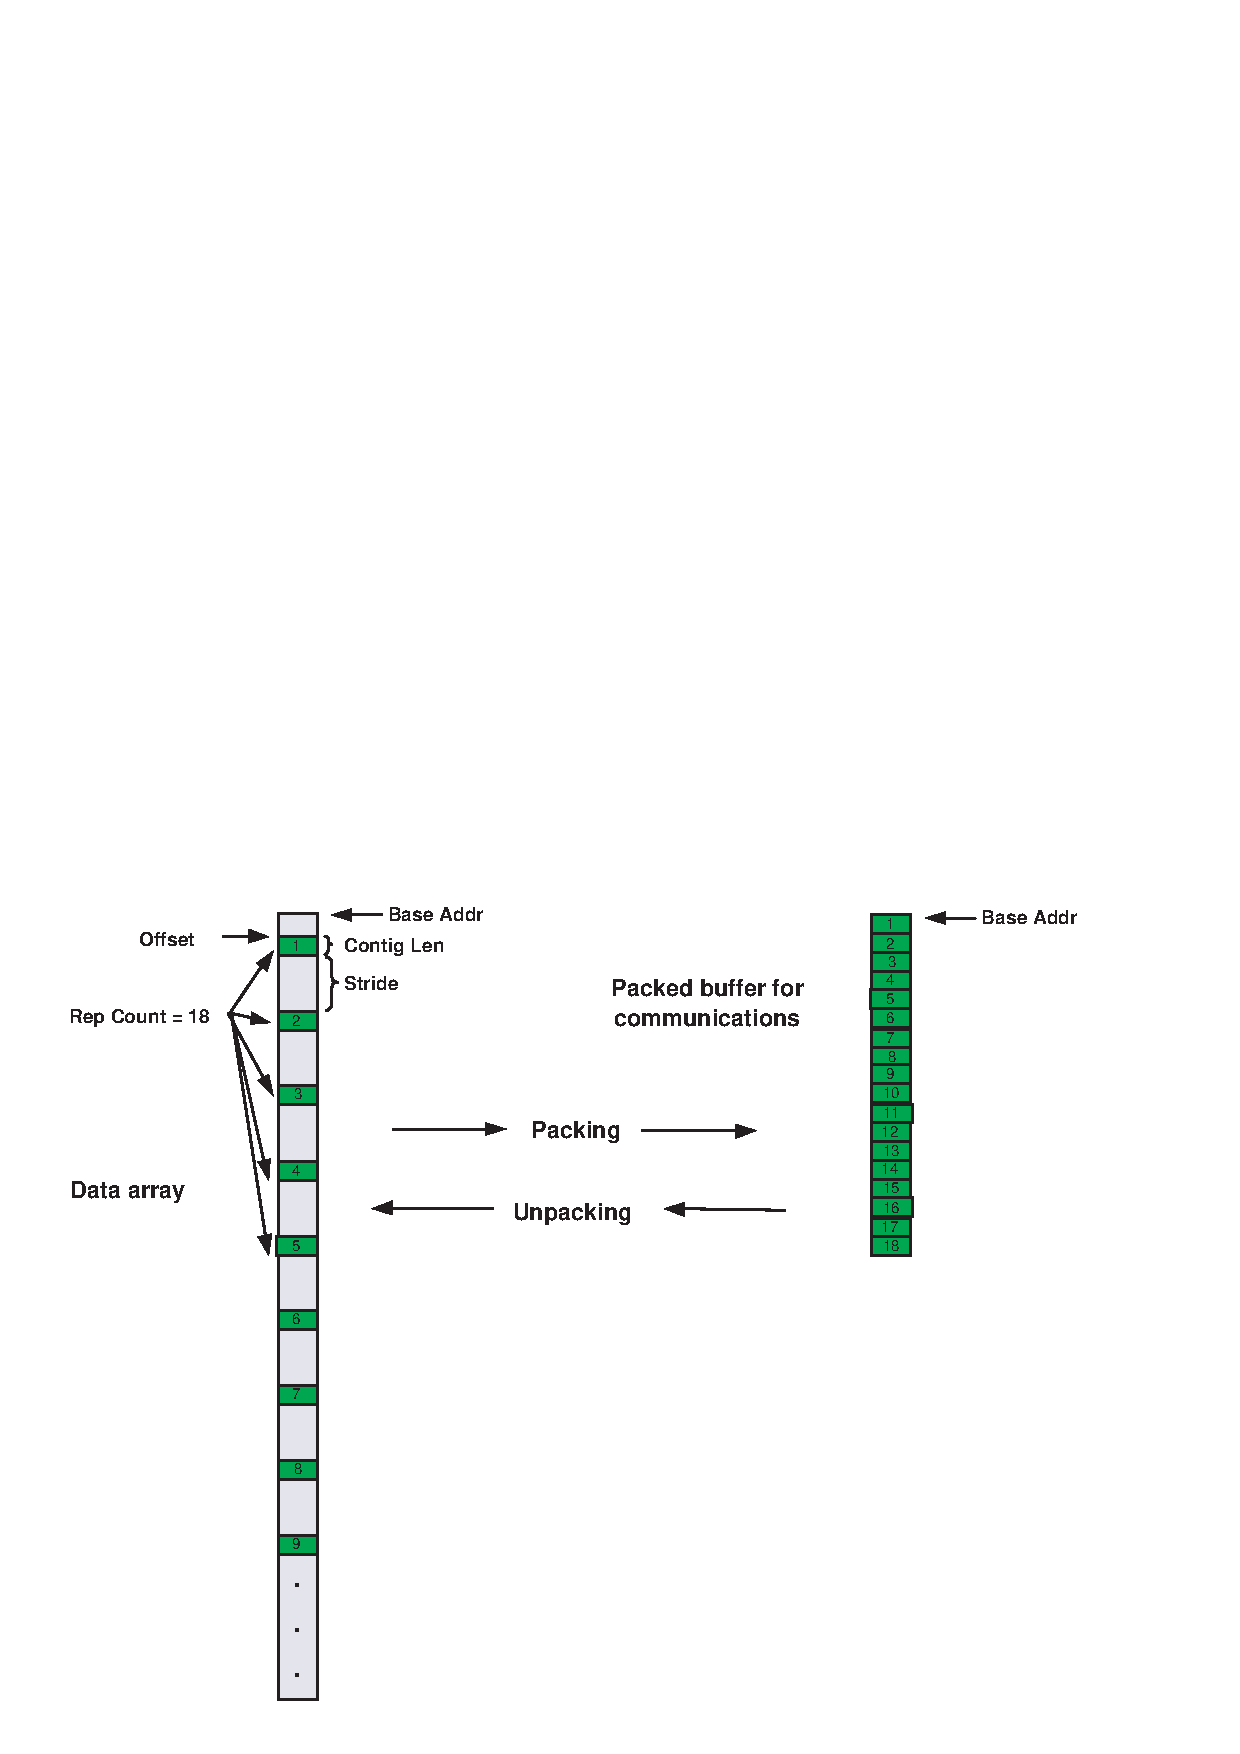
\includegraphics{Basic_pack_route}}
\caption{Often the overhead of making multiple communication calls 
outweighs the cost of copying non-contiguous data into a contiguous buffer,
sending it in a single operation, and then copying it to the final
memory locations on the receiving side.}
\label{fig:routepack}
\end{figure}
\end{center}

\begin{center}
\begin{figure}
\scalebox{0.8}{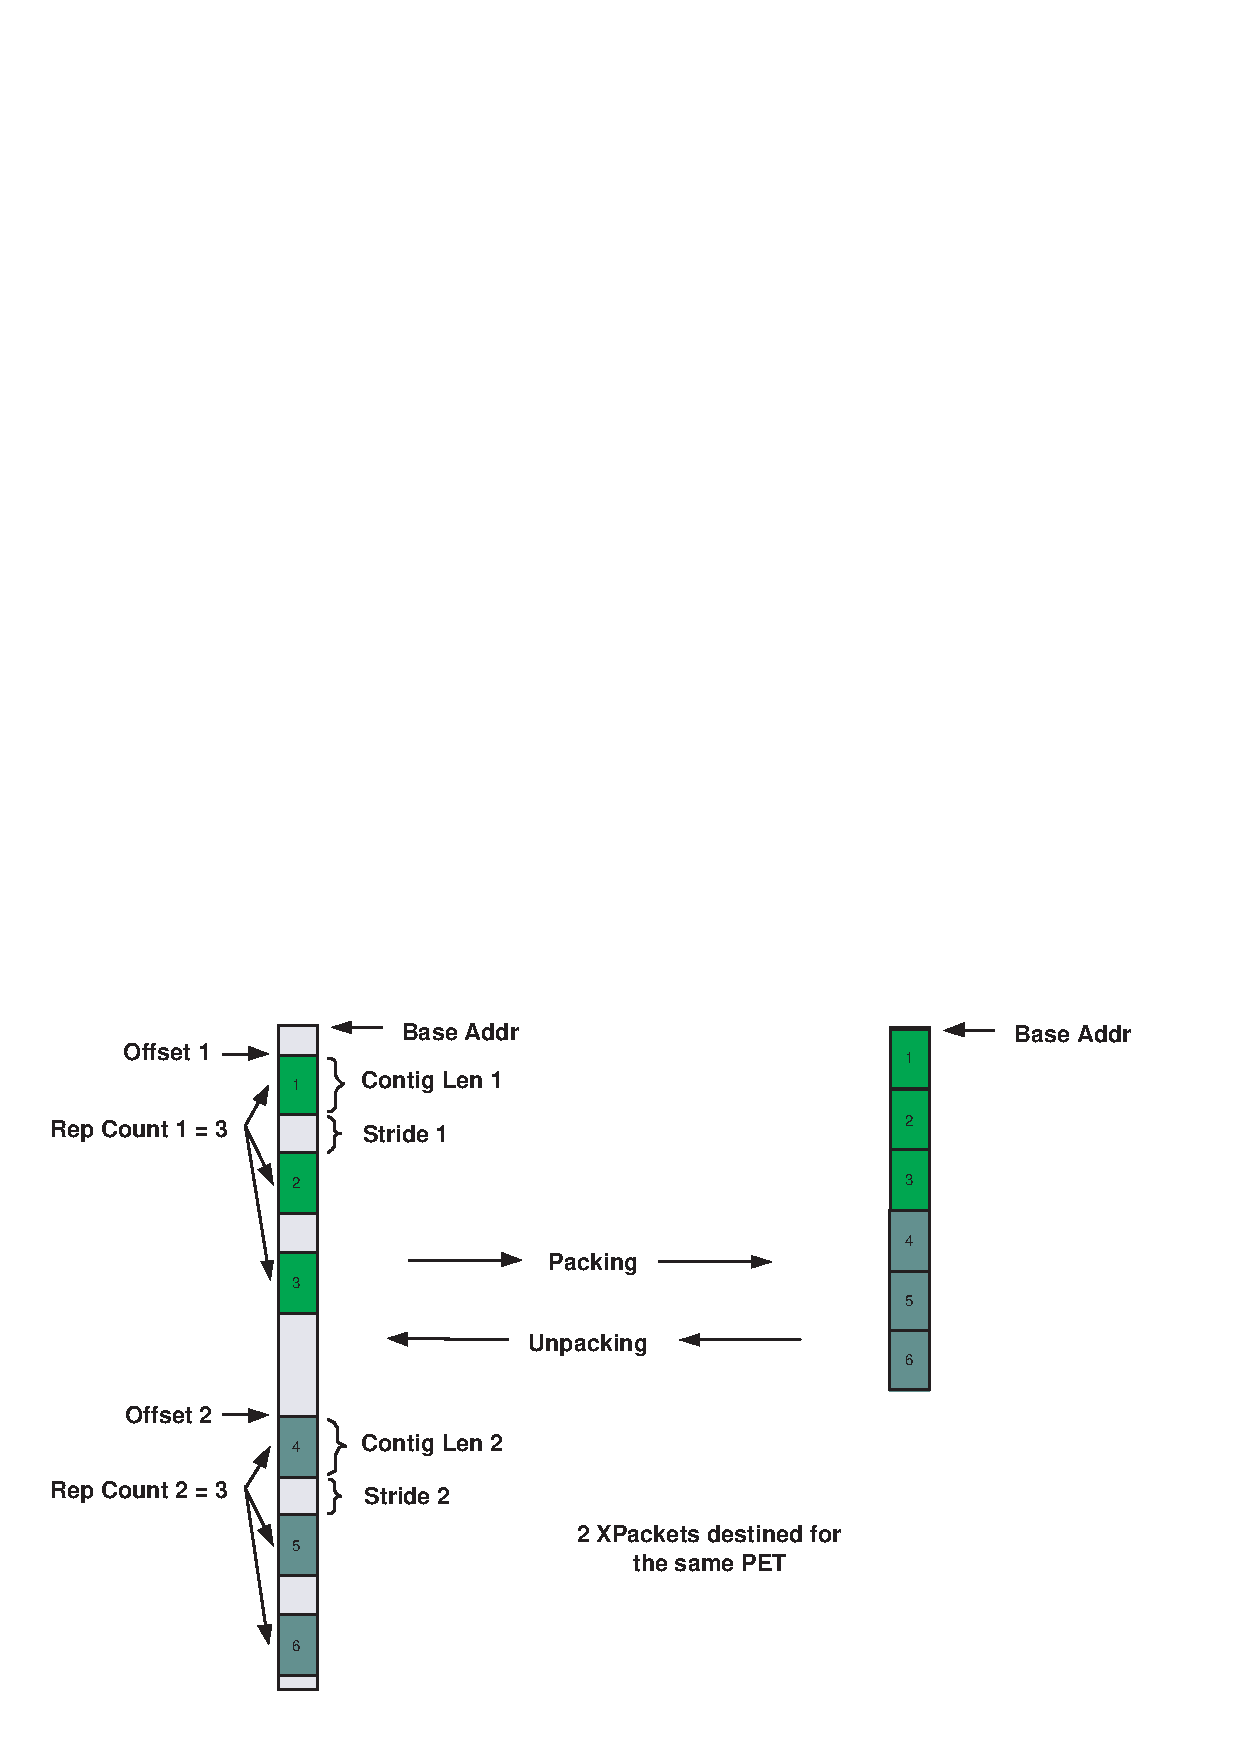
\includegraphics{Basic_2up_route}}
\caption{Once there is more than a single XPacket to pack, there
are many more interleave options.  For example, packing in the
order: 1, 4, 2, 5, 3, 6 would also be possible here.  However
the code becomes more complicated when the XPackets have different
repeat counts, and has no real performance advantage over the
straightforward packing of each XPacket in sequence.  Note that
this packing is the same whether it refers to multiple XPackets
from the same memory buffer or from multiple buffers.}
\label{fig:routepackall}
\end{figure}
\end{center}

The following options refer to the internal strategy for 
executing the route and not to whether the user-level API call
returns before the route has finished executing.  The current
system only implements user-synchronous calls; asynchronous calls
are on the to-be-written list.

\begin{enumerate}

\item[Sync] Each pair of processors exchanges data with the VM
equivalent of an MPI\_SendRecv() call, which does not return until
both the send and receive have completed.

\item[Async] Each processor executes both an asynchronous send
and asynchronous receive to the other processor and does not wait
for completion before moving on to the next communication in the
CommTable.  Then in a separate loop through the RTables, each
call is waited for in turn and when all outstanding communication
calls have completed, then the API call returns to the user.

\end{enumerate}
(Note that in the Async case it makes much more sense to iterate
through the Route table in PET order instead of the complication
of computing communication pairs and iterating in a non-sequential
order.  The code is as it is now for reasons of implementation speed
and not for any other design reason.  This would require a slightly
simpler, but separate, version of the RouteRun() subroutine.)

\item

FieldBundle-level communication calls have additional packing options
under certain circumstances.  FieldBundles are groups of Fields which
share the same Grid, but they are not required to share the same
data types, data ranks, nor relative data locations.  FieldBundles
in which these things are the same in all Fields are marked inside the
bundle code as being {\bf congruent}.  At communication store time
FieldBundles which have congruent data in all the Fields have the option
of packing all Field data together into fewer communication calls
which generally is expected to give better performance.   
Fields where the data is not of the same type or perhaps not
the same number of items (e.g. different rank, vertex-centered data
vs. cell centered data) can in theory also be packed but in fact
the code becomes more complicated, and in the case of differing
data types may cause system errors because of accessing data
on non-standard byte offsets or putting mixing integer data
with floating data and causing NaN (not a number) exceptions.
In this case, the conservative implementation strategy is to construct 
a separate Route object for each Field, all enclosed in the same
RouteHandle.  Inside the FieldBundle communication code the execution
for both types of FieldBundles is identical for the caller, but inside
the congruent FieldBundle code calls the {\tt ESMF\_RouteRun()} code
once and all communication for all Fields in the FieldBundle is done
when it returns.  The non-congruent FieldBundles execute a separate
{\tt ESMF\_RouteRun()} call for each Field and return to the user 
when all Field data have been sent/received.

There are comments in the code for an intermediate level of
optimization in which the FieldBundle code determines the smallest
number of unique types of Fields in the FieldBundle, and all same types
share the same Route object, but this has not been implemented
at this time.  Once the existing code has been in use for a while,
whether this is useful or needed may become more clear.


\item

The precompute code for all operations must have enough
information to compute which parts of the data arrays
are expected to be sent to remote PETs and also what
remote data is expected to be received by this PET.

These computations depend heavily on what type of distributed
method is being executed.  The regridding methods are described
in detail separately in the Regrid Design and Implementation Notes
section.  The halo and redistribution operations are described here.

\begin{enumerate}

\item[Halo] The total array area, which includes any halo regions,
are intersected with the computational
area of other DEs. The overlap regions are converted from index
space into memory space and stored as XPackets in the RTables.
This code must be aware of: whether the grid was defined as
periodic in any or all of the dimensions since that affects
which halo regions overlap at the grid edges; if the data
is only decomposed into a single block in any dimension (which
means it halos with itself); and if the halo region is large
enough that a halo operation may require intersection with
the N+1 neighbor in any dimension.  

\item[Redistribute]  Each DE computes the overlap
between its own computational region and all DEs in the 
remote Grid, again only working in computational area.  
The overlap regions are converted from index
space into memory space and stored as XPackets in the RTables.
After execution a redistribution, a halo operation may be required
to populate any halo regions with consistent data.

\end{enumerate}
(Note: the Redistribution code has been reimplemented to intersect
the DEs in index space and then convert the overlap region to an XPacket
representation.  Halo still converts the regions from AxisIndex to 
XPackets and then intersects the XPackets, but this code needs to be
changed to intersect in AxisIndex space and once the overlap is computed
then convert to XPackets.  Intersecting AxisIndex objects is very 
much simpler, both to understand and to execute, and more easily 
extensible to multiple dimensions than intersecting XPackets.)

\end{enumerate}

\subsection{Object Model}

The following is a simplified UML diagram showing the structure of the public
RouteHandle class.  See Appendix A, {\it A Brief Introduction to UML}, for a
translation table that lists the symbols in the diagram and their meaning.

\begin{center}
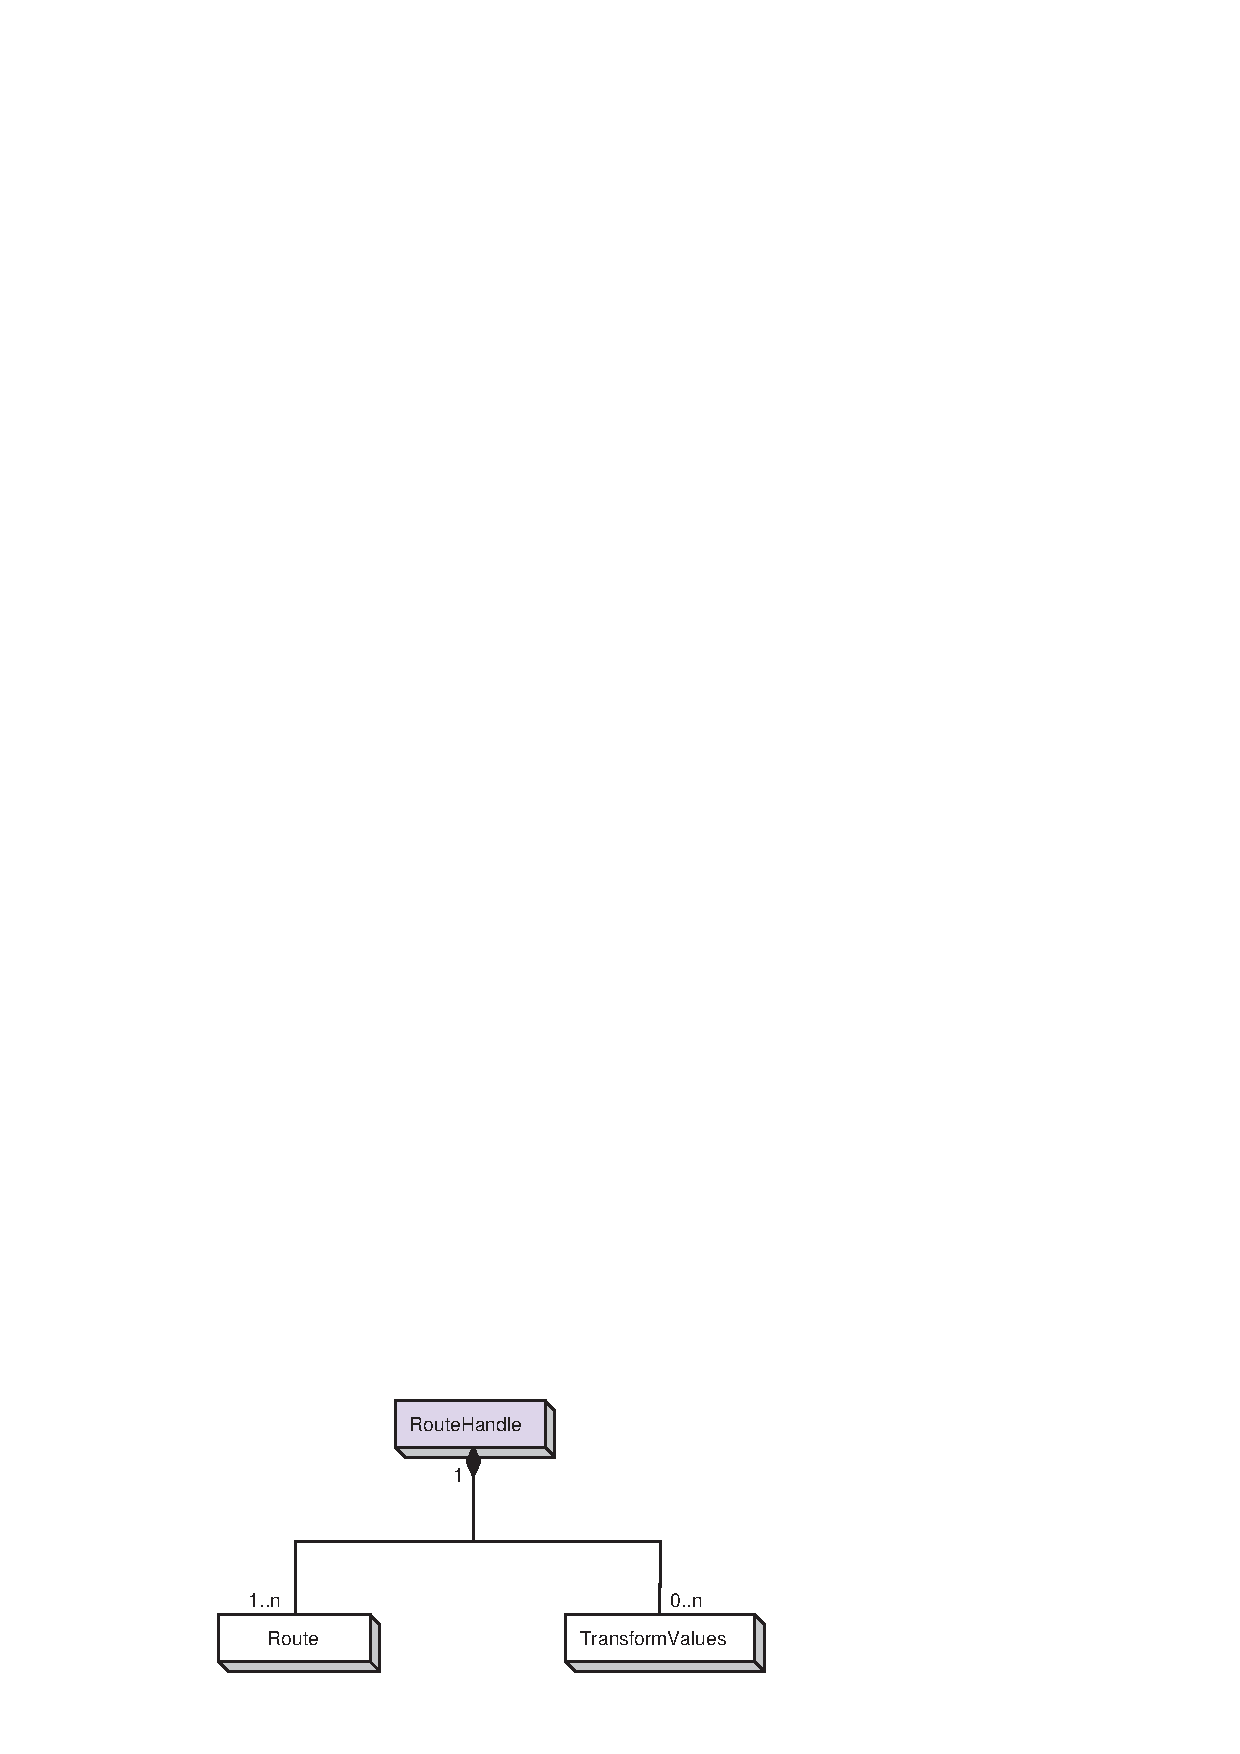
\includegraphics{RouteHandle_obj}
\end{center}


\newpage






%===============================================================================
\newpage
\begin{htmlonly}
\addcontentsline{toc}{part}{Infrastructure: Utilities}
\end{htmlonly}
\part{Infrastructure: Utilities}
\newpage
%\section{Overview of Infrastructure Utility Classes}
% $Id$
%
% Earth System Modeling Framework
% Copyright 2002-2020, University Corporation for Atmospheric Research, 
% Massachusetts Institute of Technology, Geophysical Fluid Dynamics 
% Laboratory, University of Michigan, National Centers for Environmental 
% Prediction, Los Alamos National Laboratory, Argonne National Laboratory, 
% NASA Goddard Space Flight Center.
% Licensed under the University of Illinois-NCSA License.

%TODO: This file started as an exact copy of the Fortran version of this file.
%TODO: Changes were made to correctly reflect the current status of the C API.
%TODO: Eventually this file should be removed again and replaced by a single
%TODO: generic version that can be included for both Fortran and C refdocs.

\section{Overview of Infrastructure Utility Classes}

The ESMF utilities are a set of tools for quickly assembling modeling applications.

The Time Management Library provides utilities for time and time interval representation, as well as a higher-level utility, a clock, that controls model time stepping.

The ESMF Config class provides configuration management based on NASA DAO's Inpak package, a collection of methods for accessing files containing input parameters stored in an ASCII format.

The ESMF LogErr class consists of a method for writing error, warning, and informational messages to a default Log file that is created during ESMF initialization.

The ESMF VM (Virtual Machine) class provides methods for querying information about a VM. A VM is a generic representation of hardware and system software resources. There is exactly one VM object per ESMF Component, providing the execution environment for the Component code. The VM class handles all resource management tasks for the Component class and provides a description of the underlying configuration of the compute resources used by a Component.  In addition to resource description and management, the VM class offers the lowest level of ESMF communication methods.

\newpage
%#include "../Infrastructure/Attribute/doc/Attribute_crefdoc.ctex"
% $Id$
\bodytext{BGCOLOR=white LINK=#083194 VLINK=#21004A}
% -------------------------
% Time Manager Introduction
% -------------------------
\section{Time Manager Utility}
% $Id$

The ESMF Time Manager utility includes software for time and time interval 
representation, as well as model time advancement. Since multi-component 
geophysical applications often require synchronization across 
the time management schemes of the individual components, the 
Time Manager's standard calendars and consistent time representation 
promote component interoperability.
\begin{center}  
\begin{tabular}{|p{6in}|}
\hline
\vspace{.01in}
{\bf Key Features} \\[.01in]
Drift-free timekeeping through an integer-based internal time 
representation.  Both integers and reals can be specified at the interface. \\
Support for many calendar kinds. \\
Support for both concurrent and sequential modes of component execution. \\[.03in] \hline
\end{tabular}
\end{center}

\subsection{Time Manager Classes}
There are four ESMF classes that represent time concepts:
\begin{itemize}
\item {\bf Calendar}  A Calendar can be used to keep track of the 
date as an ESMF Gridded Component advances in time. Standard calendars 
(such as Gregorian and 360-day) are supported. 
\item {\bf Time} A Time represents a time instant in a particular 
calendar, such as November 28, 1964, at 7:00pm EST in the Gregorian 
calendar.  The Time class can be used 
to represent the start and stop time of a time integration.
\item {\bf TimeInterval} TimeIntervals represent a period 
of time, such as 3 hours.  Time steps can be represented 
using TimeIntervals. 
\item {\bf Clock} Clocks collect the parameters and 
methods used for model time advancement into a convenient 
package.  A Clock can be queried for quantities such 
as current simulation time and time step.  Clock methods 
include incrementing the current time, and printing the its contents.
\end{itemize}

%\begin{center}
%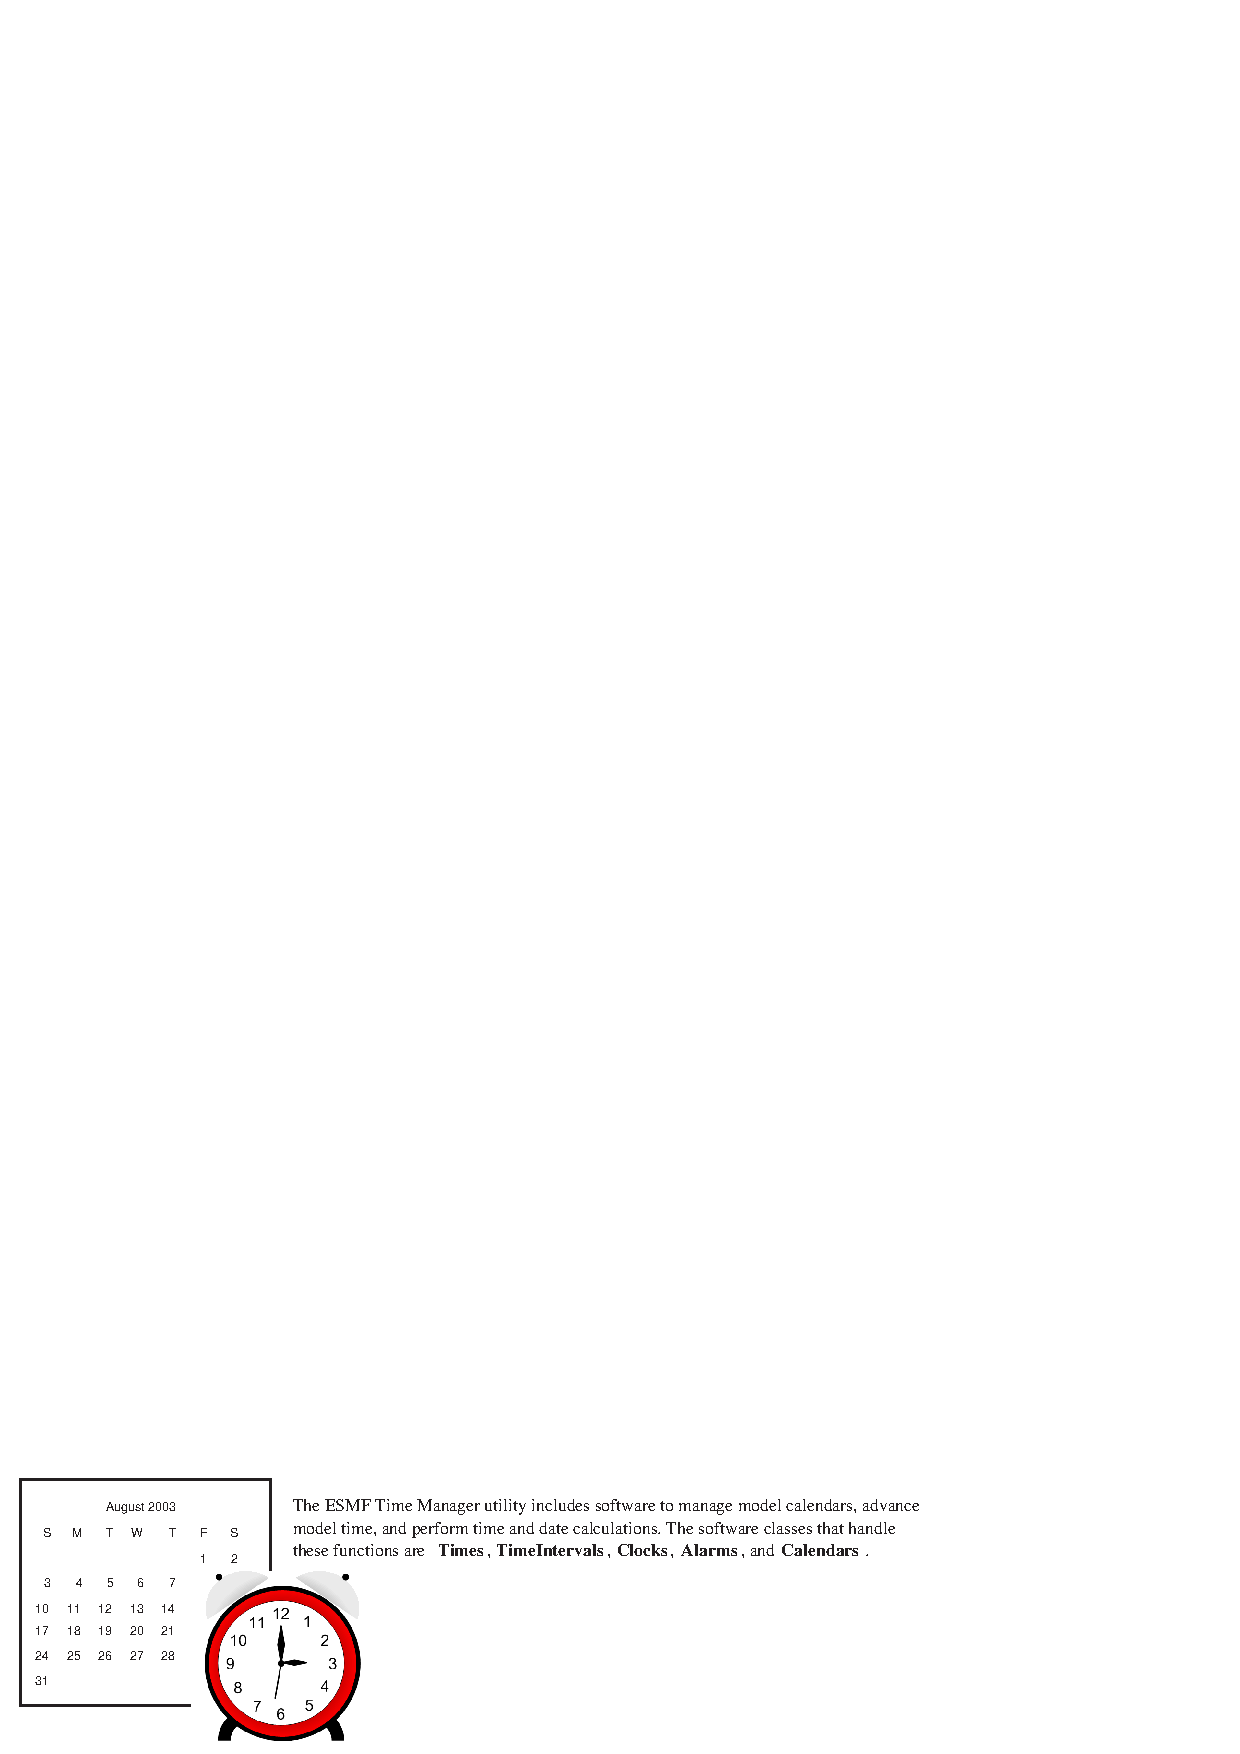
\includegraphics{TimeMgr_desc}
%\end{center}

%\newpage
%In the remainder of this section, we briefly summarize the 
%functionality that the Time Manager classes provide.  Detailed 
%descriptions and usage examples precede the API listing for each 
%class.

\subsection{Calendar}
The set of supported calendars includes:
\begin{description}
\item [Gregorian] The standard Gregorian calendar.
\item [no-leap] The Gregorian calendar with no leap years.
\item [Julian] The standard Julian date calendar.
\item [Julian Day] The standard Julian days calendar.
\item [Modified Julian Day] The Modified Julian days calendar.
\item [360-day] A 30-day-per-month, 12-month-per-year calendar.
\item [no calendar] Tracks only elapsed model time in hours, minutes, seconds.
\end{description}
See Section~\ref{sec:Calendar} for more details on supported standard 
calendars, and how to create a customized ESMF Calendar.

\subsection{Time Instants and TimeIntervals}
\label{subsec:Time Instants and TimeIntervals}
TimeIntervals and Time instants (simply called Times) are the computational 
building blocks of the Time Manager utility.  Times support different queries 
for values of individual Time components such as year and hour.
See Sections~\ref{sec:Time} and ~\ref{sec:TimeInterval}, respectively, 
for use of Times and TimeIntervals.

\subsection{Clocks}
It is useful to identify a higher-level concept to repeatedly step a Time 
forward by a TimeInterval.  We refer to this capability as a Clock, and 
include in its required features the ability to store the start and stop times 
of a model run, and to query the value of quantities such as the current time 
and the number of time steps taken.  Applications may contain 
temporary or multiple Clocks. Section~\ref{sec:Clock} describes the use of 
Clocks in detail.

%\section{Abbreviations Table}
%\newpage
\label{table:timeOpts}
\begin{center}
\begin{table}
\caption{Specifiers for Times and TimeIntervals}
\begin{tabular}{|p{1in}|p{3.5in}|}
\hline
Unit & Meaning \\
\hline\hline
{\bf <yy|yy\_i8>} & Year. \\
\hline
{\bf mm} & Month of the year. \\
\hline
{\bf dd} & Day of the month. \\
\hline
{\bf <d|d\_i8|d\_r8>} & Julian or Modified Julian day. \\
\hline
{\bf <h|h\_r8>} & Hour. \\
\hline
{\bf <m|m\_r8>} & Minute. \\
\hline
{\bf <s|s\_i8|s\_r8>} & Second. \\
\hline
{\bf <ms|ms\_r8>} & Millisecond. \\
\hline
{\bf <us|us\_r8>} & Microsecond. \\
\hline
{\bf <ns|ns\_r8>} & Nanosecond. \\
\hline
{\bf O} & Time zone offset in integer number of hours and minutes. \\
\hline
{\bf <sN|sN\_i8>} & Numerator for times of the form s {\bf $ + 
\frac{{\rm sN}}{{\rm sD}}$}, where s is seconds and s, sN, and
sD are integers.  This format provides a mechanism for supporting
exact behavior. \\
\hline
{\bf <sD|sD\_i8} & Denominator for times of the form s {\bf $ + 
\frac{{\rm sN}}{{\rm sD}}$}, where s is seconds and s, sN, and
sD are integers. \\
\hline
\end{tabular}
\end{table}
\end{center}

%\subsection{Design and Implementation Notes}
%% $Id$

\subsection{Design and Implementation Notes}
\begin{enumerate}

\item {\bf Base TimeIntervals and Times on the same integer representation.} 
It is useful to allow both TimeIntervals and Times to 
inherit from a single class, BaseTime.  In C++, this can be
implemented by using inheritance.  In Fortran, it can be implemented
by having the derived types TimeIntervals and Times
contain a derived type BaseTime.  In both cases, the 
BaseTime class can be made private and invisible to the user.

The result of this strategy is that Time Intervals and 
Times gain a consistent core representation of time as well a set
of basic methods.

The BaseTime class can be designed with a minimum number of elements
to represent any required time.  The design is based on the idea used
in the real-time POSIX 1003.1b-1993 standard.  That is, to represent
time simply as a pair of integers: one for seconds (whole) and one for
nanoseconds (fractional).  These can then be converted at the interface
level to any desired format.

For ESMF, this idea can be modified and extended, in order to handle the
requirements for a large time range (> 200,000 years) and to exactly
represent any rational fraction, not just nanoseconds.  To handle the
large time range, a 64-bit or greater integer is used for whole seconds.
Any rational fractional second is expressed using two additional integers:
a numerator and a denominator.  Both the whole seconds and fractional
numerator are signed to handle negative time intervals and instants.
For arithmetic consistency both must carry the same sign (both positive
or both negative), except, of course, for zero values.  The fractional
seconds element (numerator) is bounded with respect to whole seconds. 
If the absolute value of the
numerator becomes greater than or equal to the denominator, whole
seconds are incremented or decremented accordingly and the numerator is
reset to the remainder.  Conversions are performed upon demand by
interface methods within the TimeInterval and
Time classes.  This is done because different applications require different
representations of time intervals and time instances.  Floating point values as well as integers can be specified for the various time units in the interfaces, see Table~\ref{table:timeOpts}.  Floating point values are represented internally as integer-based rational fractions.

The BaseTime class defines increment and decrement methods for basic
TimeInterval calculations between Time instants.  It is done here rather
than in the Calendar class because it can be done with simple 
second-based arithmetic that is calendar independent.  

Comparison methods can also be defined in the BaseTime class.  These
perform equality/inequality, less than, and greater than comparisons
between any two TimeIntervals or Times.  These methods capture
the common comparison logic between TimeIntervals and Times and
hence are defined here for sharing.

\item {\bf The Time class depends on a calendar.} The Time class contains 
an internal Calendar class.  
Upon demand by a user, the results of an increment or decrement operation are 
converted to user units, which may be calendar-dependent, via methods 
obtained from their internal Calendar.

\end{enumerate}













%\subsection{Object Model}
%% $Id$

\pagebreak
\subsection{Object Model}

The following is a simplified UML diagram showing the structure of the
Time Manager utility.  See Appendix A, {\it A Brief Introduction to UML},
for a translation table that lists the symbols in the diagram and their 
meaning.

\begin{center}
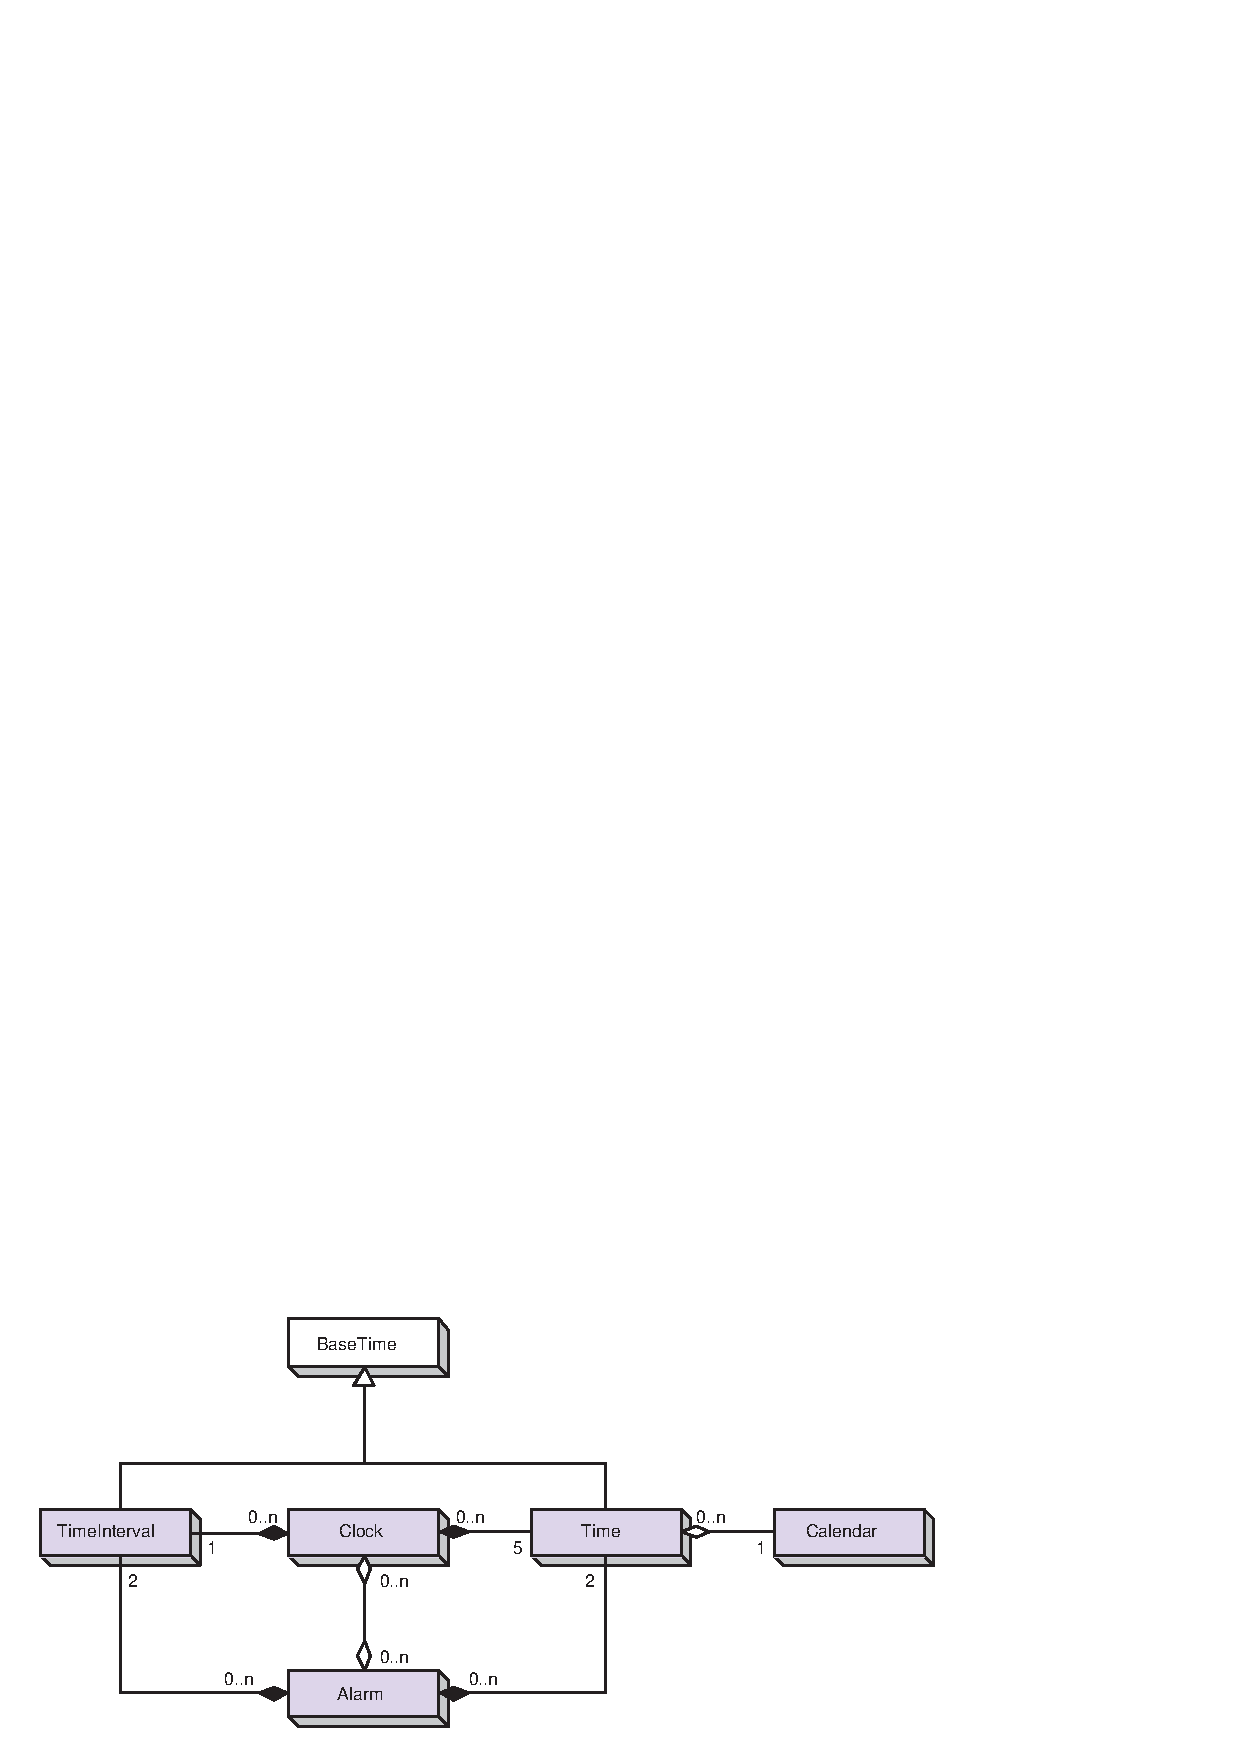
\includegraphics{TimeMgr_obj}   
\end{center}

% --------------
% Calendar Class
% --------------
\newpage
\section{Calendar Class}
\subsection{Description}
% $Id$

\label{sec:Calendar}
The Calendar class represents the standard calendars used in 
geophysical modeling:  Gregorian, Julian, Julian Day, Modified Julian Day, 
no-leap, 360-day, and no-calendar.  Brief descriptions are provided for each calendar below.

\subsection{Constants}
% $Id$

\label{subsec:Calendar_options}

\subsubsection{ESMC\_CALKIND}
\label{const:calkindflag_c}


{\sf DESCRIPTION:\\}
Supported calendar kinds.

The type of this flag is:

{\tt type(ESMF\_CalKind\_Flag)}

The valid values are:
\begin{description}
      
\item [ESMC\_CALKIND\_360DAY] 
{\it Valid range: machine limits} 
\newline In the 360-day calendar, there are 12 months, each of which has 30 days.  
Like the no-leap calendar, this is a simple approximation to the Gregorian
calendar sometimes used by modelers.

\item [ESMC\_CALKIND\_GREGORIAN] 
{\it Valid range: 3/1/4801 BC to 10/29/292,277,019,914 }
\newline The Gregorian calendar is the calendar currently in use 
throughout Western countries.  Named after Pope Gregory XIII, it is a minor 
correction to the older Julian calendar. In the Gregorian calendar every
fourth year is a leap year in which February has 29 and not 28 days;
however, years divisible by 100 are not leap years unless they are also 
divisible  by 400.  As in the Julian calendar, days begin at midnight.

\item [ESMC\_CALKIND\_JULIAN]
{\it Valid range: 3/1/4713 BC to 4/24/292,271,018,333 } 
\newline The Julian calendar was introduced by Julius Caesar in 46 B.C., and 
reached its final form in 4 A.D.  The Julian calendar differs from the 
Gregorian only in the determination of leap years, lacking the correction 
for years divisible by 100 and 400 in the Gregorian calendar.  In the Julian 
calendar, any year is a leap year if divisible by 4.  Days are considered to 
begin at midnight.

\item [ESMC\_CALKIND\_JULIANDAY] 
{\it Valid range:  +/- 1x10$^{14}$} 
\newline Julian days simply enumerate the days and fraction of a day which 
have elapsed since the start of the Julian era, defined as beginning at noon 
on Monday, 1st January of year 4713 B.C. in the Julian calendar.  Julian days, 
unlike the dates in the Julian and Gregorian calendars, begin at noon.

\item [ESMC\_CALKIND\_MODJULIANDAY]
{\it Valid range:  +/- 1x10$^{14}$}
\newline The Modified Julian Day (MJD) was introduced by space scientists in
 the late 1950's.  It is defined as an offset from the Julian Day (JD):

MJD = JD - 2400000.5

The half day is subtracted so that the day starts at midnight.

\item [ESMC\_CALKIND\_NOCALENDAR] 
{\it Valid range: machine limits}
\newline The no-calendar option simply tracks the elapsed model time in seconds.

\item [ESMC\_CALKIND\_NOLEAP]
{\it Valid range: machine limits} 
\newline The no-leap calendar is the Gregorian calendar with no leap years - 
February is always assumed to have 28 days.  Modelers sometimes use this 
calendar as a simple, close approximation to the Gregorian calendar.

\end{description}

%\subsection{Use and Examples}
%% $Id$

In most multi-component Earth system applications, the timekeeping in 
each component 
must refer to the same standard calendar in order for the components 
to properly synchronize.  It therefore makes sense to create as few 
ESMF Calendars as possible, preferably one per application.
A typical strategy would be to create a single Calendar at the start
of an application, and use that Calendar in all subsequent calls that
accept a Calendar, such as {\tt ESMF\_TimeSet}.

The following example shows how to set up an ESMF Calendar.  

%%                **** IMPORTANT NOTICE *****
% This LaTeX file has been automatically produced by ProTeX v. 1.1
% Any changes made to this file will likely be lost next time
% this file is regenerated from its source. Send questions 
% to Arlindo da Silva, dasilva@gsfc.nasa.gov
 
\setlength{\oldparskip}{\parskip}
\setlength{\parskip}{1.5ex}
\setlength{\oldparindent}{\parindent}
\setlength{\parindent}{0pt}
\setlength{\oldbaselineskip}{\baselineskip}
\setlength{\baselineskip}{11pt}
 
%--------------------- SHORT-HAND MACROS ----------------------
\def\bv{\begin{verbatim}}
\def\ev{\end{verbatim}}
\def\be{\begin{equation}}
\def\ee{\end{equation}}
\def\bea{\begin{eqnarray}}
\def\eea{\end{eqnarray}}
\def\bi{\begin{itemize}}
\def\ei{\end{itemize}}
\def\bn{\begin{enumerate}}
\def\en{\end{enumerate}}
\def\bd{\begin{description}}
\def\ed{\end{description}}
\def\({\left (}
\def\){\right )}
\def\[{\left [}
\def\]{\right ]}
\def\<{\left  \langle}
\def\>{\right \rangle}
\def\cI{{\cal I}}
\def\diag{\mathop{\rm diag}}
\def\tr{\mathop{\rm tr}}
%-------------------------------------------------------------

\markboth{Left}{Source File: ESMF\_CalendarEx.F90,  Date: Tue May  5 20:59:34 MDT 2020
}

 
%/////////////////////////////////////////////////////////////

 \begin{verbatim}
! !PROGRAM: ESMF_CalendarEx - Calendar creation examples
!
! !DESCRIPTION:
!
! This program shows examples of how to create different calendar kinds
!-----------------------------------------------------------------------------
#include "ESMF.h"

      ! ESMF Framework module
      use ESMF
      use ESMF_TestMod
      implicit none

      ! instantiate calendars
      type(ESMF_Calendar) :: gregorianCalendar
      type(ESMF_Calendar) :: julianDayCalendar
      type(ESMF_Calendar) :: marsCalendar

      ! local variables for Get methods
      integer :: sols
      integer(ESMF_KIND_I8) :: dl
      type(ESMF_Time) :: time, marsTime
      type(ESMF_TimeInterval) :: marsTimeStep

      ! return code
      integer:: rc
 
\end{verbatim}
 
%/////////////////////////////////////////////////////////////

 \begin{verbatim}
      ! initialize ESMF framework
      call ESMF_Initialize(defaultlogfilename="CalendarEx.Log", &
                    logkindflag=ESMF_LOGKIND_MULTI, rc=rc)
 
\end{verbatim}
 
%/////////////////////////////////////////////////////////////

  \subsubsection{Calendar creation}
 
   This example shows how to create three {\tt ESMF\_Calendars}. 
%/////////////////////////////////////////////////////////////

 \begin{verbatim}
      ! create a Gregorian calendar
      gregorianCalendar = ESMF_CalendarCreate(ESMF_CALKIND_GREGORIAN, &
                                              name="Gregorian", rc=rc)
 
\end{verbatim}
 
%/////////////////////////////////////////////////////////////

 \begin{verbatim}
      ! create a Julian Day calendar
      julianDayCalendar = ESMF_CalendarCreate(ESMF_CALKIND_JULIANDAY, &
                                              name="JulianDay", rc=rc)
 
\end{verbatim}
 
%/////////////////////////////////////////////////////////////

 \begin{verbatim}
      ! create a Custom calendar for the planet Mars
      ! 1 Mars solar day = 24 hours, 39 minutes, 35 seconds = 88775 seconds
      ! 1 Mars solar year = 668.5921 Mars solar days = 668 5921/10000 sols/year
      ! http://www.giss.nasa.gov/research/briefs/allison_02
      ! http://www.giss.nasa.gov/tools/mars24/help/notes.html
      marsCalendar = ESMF_CalendarCreate(secondsPerDay=88775, &
                                         daysPerYear=668, &
                                         daysPerYearDn=5921, &
                                         daysPerYearDd=10000, &
                                         name="MarsCalendar", rc=rc)
 
\end{verbatim}
 
%/////////////////////////////////////////////////////////////

  \subsubsection{Calendar comparison}
 
   This example shows how to compare an {\tt ESMF\_Calendar} with a known
   calendar kind. 
%/////////////////////////////////////////////////////////////

 \begin{verbatim}
      ! compare calendar kind against a known type
      if (gregorianCalendar == ESMF_CALKIND_GREGORIAN) then
        print *, "gregorianCalendar is of type ESMF_CALKIND_GREGORIAN."
      else
        print *, "gregorianCalendar is not of type ESMF_CALKIND_GREGORIAN."
      end if
 
\end{verbatim}
 
%/////////////////////////////////////////////////////////////

  \subsubsection{Time conversion between Calendars}
 
   This example shows how to convert a time from one {\tt ESMF\_Calendar}
   to another. 
%/////////////////////////////////////////////////////////////

 \begin{verbatim}
      call ESMF_TimeSet(time, yy=2004, mm=4, dd=17, &
                        calendar=gregorianCalendar, rc=rc)
 
\end{verbatim}
 
%/////////////////////////////////////////////////////////////

 \begin{verbatim}
      ! switch time's calendar to perform conversion
      call ESMF_TimeSet(time, calendar=julianDayCalendar, rc=rc)
 
\end{verbatim}
 
%/////////////////////////////////////////////////////////////

 \begin{verbatim}
      call ESMF_TimeGet(time, d_i8=dl, rc=rc)
      print *, "Gregorian date 2004/4/17 is ", dl, &
               " days in the Julian Day calendar."
 
\end{verbatim}
 
%/////////////////////////////////////////////////////////////

  \subsubsection{Add a time interval to a time on a Calendar}
 
   This example shows how to increment a time using a custom {\tt ESMF\_Calendar}. 
%/////////////////////////////////////////////////////////////

 \begin{verbatim}
      ! Set a time to Mars solar year 3, sol 100
      call ESMF_TimeSet(marsTime, yy=3, d=100, &
                        calendar=marsCalendar, rc=rc)
 
\end{verbatim}
 
%/////////////////////////////////////////////////////////////

 \begin{verbatim}
      ! Set a 1 solar year time step
      call ESMF_TimeIntervalSet(marsTimeStep, yy=1, rc=rc)
 
\end{verbatim}
 
%/////////////////////////////////////////////////////////////

 \begin{verbatim}
      ! Perform the increment
      marsTime = marsTime + marsTimeStep
 
\end{verbatim}
 
%/////////////////////////////////////////////////////////////

 \begin{verbatim}
      ! Get the result in sols (2774 = (3+1)*668.5921 + 100)
      call ESMF_TimeGet(marsTime, d=sols, rc=rc)
      print *, "For Mars, 3 solar years, 100 sols + 1 solar year = ", &
                sols, "sols."
 
\end{verbatim}
 
%/////////////////////////////////////////////////////////////

  \subsubsection{Calendar destruction}
 
   This example shows how to destroy three {\tt ESMF\_Calendars}. 
%/////////////////////////////////////////////////////////////

 \begin{verbatim}
      call ESMF_CalendarDestroy(julianDayCalendar, rc=rc)
 
\end{verbatim}
 
%/////////////////////////////////////////////////////////////

 \begin{verbatim}
      call ESMF_CalendarDestroy(gregorianCalendar, rc=rc)
 
\end{verbatim}
 
%/////////////////////////////////////////////////////////////

 \begin{verbatim}
      call ESMF_CalendarDestroy(marsCalendar, rc=rc)
 
\end{verbatim}
 
%/////////////////////////////////////////////////////////////

 \begin{verbatim}
      ! finalize ESMF framework
      call ESMF_Finalize(rc=rc)
 
\end{verbatim}
 
%/////////////////////////////////////////////////////////////

 \begin{verbatim}
      end program ESMF_CalendarEx
 
\end{verbatim}

%...............................................................
\setlength{\parskip}{\oldparskip}
\setlength{\parindent}{\oldparindent}
\setlength{\baselineskip}{\oldbaselineskip}

%\subsection{Restrictions and Future Work}
%% $Id$

\label{subsec:Calendar_rest}

\begin{enumerate}

\item {\bf Months per year set to 12.} Due to the requirement of only Earth modeling, the number of months per year is hard-coded at 12.  However, for easy modification, this is implemented via a C preprocessor \#define MONTHS\_PER\_YEAR in ESMCI\_Calendar.h.

\item {\bf Calendar date conversions.} Date conversions are currently defined between the Gregorian, Julian, Julian Day, and Modified Julian Day calendars. Further research and work would need to be done to determine conversion algorithms with and between the other calendars:  No Leap, 360 Day, and Custom.

\item {\bf ESMF\_CALKIND\_CUSTOM.} Currently, there is no provision for a custom calendar to define a leap year rule, so {\tt ESMF\_CalendarIsLeapYear()} will always return {\tt .false.} in this case.  However, the arguments {\tt daysPerYear}, {\tt daysPerYearDn}, and {\tt daysPerYearDd} in {\tt ESMF\_CalendarCreate()} and {\tt ESMF\_CalendarSet()} can be used to set a fractional number of days per year, for example, 365.25 = 365 25/100.  Also, if further timekeeping precision is required, fractional and/or floating point {\tt secondsPerDay} and {\tt secondsPerYear} could be added to the interfaces {\tt ESMF\_CalendarCreate()}, {\tt ESMF\_CalendarSet()}, and {\tt ESMF\_CalendarGet()} and implemented.

\end{enumerate}

%\subsection{Design and Implementation Notes}
%% $Id$

\subsection{Implementation Notes}

The algorithm for computing between Gregorian dates and Julian days is given 
in Fliegel and Flandern ~\cite{Fli68}.

The algorithm for computing between Julian dates and Julian days is given 
in Hatcher ~\cite{Hat84}.

The {\tt Calendar} class defines two methods for converting in both
directions between the core {\tt BaseTime} class representation and a
calendar date.  Calculations of time intervals (deltas) between
time instants is done by the base class {\tt BaseTime} in the core units
of seconds and fractional seconds.  Thus,  a calendar is only needed for
converting core time to calendar time and vice versa.

\subsection{Class API}
%                **** IMPORTANT NOTICE *****
% This LaTeX file has been automatically produced by ProTeX v. 1.1
% Any changes made to this file will likely be lost next time
% this file is regenerated from its source. Send questions 
% to Arlindo da Silva, dasilva@gsfc.nasa.gov
 
\setlength{\oldparskip}{\parskip}
\setlength{\parskip}{1.5ex}
\setlength{\oldparindent}{\parindent}
\setlength{\parindent}{0pt}
\setlength{\oldbaselineskip}{\baselineskip}
\setlength{\baselineskip}{11pt}
 
%--------------------- SHORT-HAND MACROS ----------------------
\def\bv{\begin{verbatim}}
\def\ev{\end{verbatim}}
\def\be{\begin{equation}}
\def\ee{\end{equation}}
\def\bea{\begin{eqnarray}}
\def\eea{\end{eqnarray}}
\def\bi{\begin{itemize}}
\def\ei{\end{itemize}}
\def\bn{\begin{enumerate}}
\def\en{\end{enumerate}}
\def\bd{\begin{description}}
\def\ed{\end{description}}
\def\({\left (}
\def\){\right )}
\def\[{\left [}
\def\]{\right ]}
\def\<{\left  \langle}
\def\>{\right \rangle}
\def\cI{{\cal I}}
\def\diag{\mathop{\rm diag}}
\def\tr{\mathop{\rm tr}}
%-------------------------------------------------------------

\markboth{Left}{Source File: ESMC\_Calendar.h,  Date: Tue May  5 20:59:33 MDT 2020
}

 
%/////////////////////////////////////////////////////////////
\subsubsection [ESMC\_CalendarCreate] {ESMC\_CalendarCreate - Create a Calendar}


  
\bigskip{\sf INTERFACE:}
\begin{verbatim} ESMC_Calendar ESMC_CalendarCreate(
   const char *name,                      // in
   enum ESMC_CalKind_Flag calkindflag,    // in
   int *rc                                // out
 );
 \end{verbatim}{\em RETURN VALUE:}
\begin{verbatim}    Newly created ESMC_Calendar object.\end{verbatim}
{\sf DESCRIPTION:\\ }


  
    Creates and sets a {\tt ESMC\_Calendar} object to the given built-in
    {\tt ESMC\_CalKind\_Flag}. 
  
    The arguments are:
    \begin{description}
    \item[{[name]}]
      The name for the newly created Calendar.  If not specified, i.e. NULL,
      a default unique name will be generated: "CalendarNNN" where NNN
      is a unique sequence number from 001 to 999.
    \item[calkindflag]
      The built-in {\tt ESMC\_CalKind\_Flag}.  Valid values are:
      \newline
      {\tt ESMC\_CALKIND\_360DAY}, 
      \newline
      {\tt ESMC\_CALKIND\_GREGORIAN},
      \newline
      {\tt ESMC\_CALKIND\_JULIAN}, 
      \newline
      {\tt ESMC\_CALKIND\_JULIANDAY},
      \newline
      {\tt ESMC\_CALKIND\_MODJULIANDAY}, 
      \newline
      {\tt ESMC\_CALKIND\_NOCALENDAR},
      \newline
      and {\tt ESMC\_CALKIND\_NOLEAP}.
      \newline
      See Section ~\ref{subsec:Calendar_options} for a description of each
      calendar kind.
    \item[{[rc]}]
      Return code; equals {\tt ESMF\_SUCCESS} if there are no errors.
    \end{description}
   
%/////////////////////////////////////////////////////////////
 
\mbox{}\hrulefill\ 
 
\subsubsection [ESMC\_CalendarDestroy] {ESMC\_CalendarDestroy - Destroy a Calendar}


  
\bigskip{\sf INTERFACE:}
\begin{verbatim} int ESMC_CalendarDestroy(
   ESMC_Calendar *calendar   // inout
 );
 \end{verbatim}{\em RETURN VALUE:}
\begin{verbatim}    Return code; equals ESMF_SUCCESS if there are no errors.\end{verbatim}
{\sf DESCRIPTION:\\ }


  
    Releases all resources associated with this {\tt ESMC\_Calendar}.
  
    The arguments are:
    \begin{description}
    \item[calendar]
      Destroy contents of this {\tt ESMC\_Calendar}.
    \end{description}
   
%/////////////////////////////////////////////////////////////
 
\mbox{}\hrulefill\ 
 
\subsubsection [ESMC\_CalendarPrint] {ESMC\_CalendarPrint - Print a Calendar}


  
\bigskip{\sf INTERFACE:}
\begin{verbatim} int ESMC_CalendarPrint(
   ESMC_Calendar calendar   // in
 );
 \end{verbatim}{\em RETURN VALUE:}
\begin{verbatim}    Return code; equals ESMF_SUCCESS if there are no errors.\end{verbatim}
{\sf DESCRIPTION:\\ }


    Prints out an {\tt ESMC\_Calendar}'s properties to {\tt stdio}, 
    in support of testing and debugging.
  
    The arguments are:
    \begin{description}
    \item[calendar]
      {\tt ESMC\_Calendar} object to be printed.
    \end{description}
  
%...............................................................
\setlength{\parskip}{\oldparskip}
\setlength{\parindent}{\oldparindent}
\setlength{\baselineskip}{\oldbaselineskip}

% ----------
% Time Class
% ----------
\newpage
\section{Time Class}
\subsection{Description}
% $Id$
\label{sec:Time}

A Time represents a specific point in time.

There are Time methods defined for setting and getting a Time.

A Time that is specified in hours does not need to be associated with a 
standard calendar; use ESMC\_CALKIND\_NOCALENDAR.  A Time whose specification 
includes time units of a year must be associated with a standard calendar. 
The ESMF representation of a calendar, the Calendar class, is described in 
Section~\ref{sec:Calendar}.  The {\tt ESMC\_TimeSet} method is used to 
initialize a Time as well as associate it with a Calendar.  If a Time method 
is invoked in which a Calendar is necessary and one has not been set, the 
ESMF method will return an error condition.

In the ESMF the TimeInterval class is used to represent time periods. 
This class is frequently used in combination with the Time class. 
The Clock class, for example, advances model time by incrementing a 
Time with a TimeInterval. 

%\subsection{Use and Examples}
%% $Id$

Times are most frequently used to represent start, stop, and current 
model times.  The following examples show how to create, initialize, and
manipulate {\tt Time}.



%%                **** IMPORTANT NOTICE *****
% This LaTeX file has been automatically produced by ProTeX v. 1.1
% Any changes made to this file will likely be lost next time
% this file is regenerated from its source. Send questions 
% to Arlindo da Silva, dasilva@gsfc.nasa.gov
 
\setlength{\oldparskip}{\parskip}
\setlength{\parskip}{1.5ex}
\setlength{\oldparindent}{\parindent}
\setlength{\parindent}{0pt}
\setlength{\oldbaselineskip}{\baselineskip}
\setlength{\baselineskip}{11pt}
 
%--------------------- SHORT-HAND MACROS ----------------------
\def\bv{\begin{verbatim}}
\def\ev{\end{verbatim}}
\def\be{\begin{equation}}
\def\ee{\end{equation}}
\def\bea{\begin{eqnarray}}
\def\eea{\end{eqnarray}}
\def\bi{\begin{itemize}}
\def\ei{\end{itemize}}
\def\bn{\begin{enumerate}}
\def\en{\end{enumerate}}
\def\bd{\begin{description}}
\def\ed{\end{description}}
\def\({\left (}
\def\){\right )}
\def\[{\left [}
\def\]{\right ]}
\def\<{\left  \langle}
\def\>{\right \rangle}
\def\cI{{\cal I}}
\def\diag{\mathop{\rm diag}}
\def\tr{\mathop{\rm tr}}
%-------------------------------------------------------------

\markboth{Left}{Source File: ESMF\_TimeEx.F90,  Date: Tue May  5 20:59:34 MDT 2020
}

 
%/////////////////////////////////////////////////////////////

 \begin{verbatim}
! !PROGRAM: ESMF_TimeEx - Time initialization and manipulation examples
!
! !DESCRIPTION:
!
! This program shows examples of Time initialization and manipulation
!-----------------------------------------------------------------------------
#include "ESMF.h"

      ! ESMF Framework module
      use ESMF
      use ESMF_TestMod
      implicit none

      ! instantiate two times
      type(ESMF_Time) :: time1, time2

      type(ESMF_VM) :: vm

      ! instantiate a time interval
      type(ESMF_TimeInterval) :: timeinterval1

      ! local variables for Get methods
      integer :: YY, MM, DD, H, M, S

      ! return code
      integer:: rc
 
\end{verbatim}
 
%/////////////////////////////////////////////////////////////

 \begin{verbatim}
      ! initialize ESMF framework
      call ESMF_Initialize(vm=vm, defaultCalKind=ESMF_CALKIND_GREGORIAN, &
        defaultlogfilename="TimeEx.Log", &
        logkindflag=ESMF_LOGKIND_MULTI, rc=rc)
 
\end{verbatim}
 
%/////////////////////////////////////////////////////////////

  \subsubsection{Time initialization}
 
   This example shows how to initialize an {\tt ESMF\_Time}. 
%/////////////////////////////////////////////////////////////

 \begin{verbatim}
      ! initialize time1 to 2/28/2000 2:24:45
      call ESMF_TimeSet(time1, yy=2000, mm=2, dd=28, h=2, m=24, s=45, rc=rc)
 
\end{verbatim}
 
%/////////////////////////////////////////////////////////////

 \begin{verbatim}
      print *, "Time1 = "
      call ESMF_TimePrint(time1, options="string", rc=rc)
 
\end{verbatim}
 
%/////////////////////////////////////////////////////////////

  \subsubsection{Time increment}
 
   This example shows how to increment an {\tt ESMF\_Time} by
   an {\tt ESMF\_TimeInterval}. 
%/////////////////////////////////////////////////////////////

 \begin{verbatim}
      ! initialize a time interval to 2 days, 8 hours, 36 minutes, 15 seconds
      call ESMF_TimeIntervalSet(timeinterval1, d=2, h=8, m=36, s=15, rc=rc)
 
\end{verbatim}
 
%/////////////////////////////////////////////////////////////

 \begin{verbatim}
      print *, "Timeinterval1 = "
      call ESMF_TimeIntervalPrint(timeinterval1, options="string", rc=rc)
 
\end{verbatim}
 
%/////////////////////////////////////////////////////////////

 \begin{verbatim}
      ! increment time1 with timeinterval1
      time2 = time1 + timeinterval1

      call ESMF_TimeGet(time2, yy=YY, mm=MM, dd=DD, h=H, m=M, s=S, rc=rc)
      print *, "time2 = time1 + timeinterval1 = ", YY, "/", MM, "/", DD, &
               " ",  H, ":", M, ":", S
 
\end{verbatim}
 
%/////////////////////////////////////////////////////////////

  \subsubsection{Time comparison}
 
   This example shows how to compare two {\tt ESMF\_Times}. 
%/////////////////////////////////////////////////////////////

 \begin{verbatim}
      if (time2 > time1) then
        print *, "time2 is larger than time1"
      else
        print *, "time1 is smaller than or equal to time2"
      endif

 
\end{verbatim}
 
%/////////////////////////////////////////////////////////////

 \begin{verbatim}
      ! finalize ESMF framework
      call ESMF_Finalize(rc=rc)
 
\end{verbatim}
 
%/////////////////////////////////////////////////////////////

 \begin{verbatim}
      end program ESMF_TimeEx
 
\end{verbatim}

%...............................................................
\setlength{\parskip}{\oldparskip}
\setlength{\parindent}{\oldparindent}
\setlength{\baselineskip}{\oldbaselineskip}

%\subsection{Restrictions and Future Work}
%% $Id$

\begin{enumerate}

\item {\bf Limits on size and resolution of Time.}  The limits on the size and 
resolution of the time representation are based on the
64-bit integer types used.  For seconds, a signed 64-bit integer
will have a range of +/- $2^{63}$-1, or +/- 9,223,372,036,854,775,807.  This
corresponds to a maximum size of +/- ($2^{63}$-1)/(86400 * 365.25) or
+/- 292,271,023,045 years.

\begin{sloppypar}
For fractional seconds, a signed 64-bit integer will handle a resolution of
+/- $2^{31}$-1, or +/- 9,223,372,036,854,775,807 parts of a second.
\end{sloppypar}

\end{enumerate}

\subsection{Class API}
%                **** IMPORTANT NOTICE *****
% This LaTeX file has been automatically produced by ProTeX v. 1.1
% Any changes made to this file will likely be lost next time
% this file is regenerated from its source. Send questions 
% to Arlindo da Silva, dasilva@gsfc.nasa.gov
 
\setlength{\oldparskip}{\parskip}
\setlength{\parskip}{1.5ex}
\setlength{\oldparindent}{\parindent}
\setlength{\parindent}{0pt}
\setlength{\oldbaselineskip}{\baselineskip}
\setlength{\baselineskip}{11pt}
 
%--------------------- SHORT-HAND MACROS ----------------------
\def\bv{\begin{verbatim}}
\def\ev{\end{verbatim}}
\def\be{\begin{equation}}
\def\ee{\end{equation}}
\def\bea{\begin{eqnarray}}
\def\eea{\end{eqnarray}}
\def\bi{\begin{itemize}}
\def\ei{\end{itemize}}
\def\bn{\begin{enumerate}}
\def\en{\end{enumerate}}
\def\bd{\begin{description}}
\def\ed{\end{description}}
\def\({\left (}
\def\){\right )}
\def\[{\left [}
\def\]{\right ]}
\def\<{\left  \langle}
\def\>{\right \rangle}
\def\cI{{\cal I}}
\def\diag{\mathop{\rm diag}}
\def\tr{\mathop{\rm tr}}
%-------------------------------------------------------------

\markboth{Left}{Source File: ESMC\_Time.h,  Date: Tue May  5 20:59:34 MDT 2020
}

 
%/////////////////////////////////////////////////////////////
\subsubsection [ESMC\_TimeGet] {ESMC\_TimeGet - Get a Time value}


  
\bigskip{\sf INTERFACE:}
\begin{verbatim} int ESMC_TimeGet(
   ESMC_Time time,                         // in
   ESMC_I4 *yy,                            // out
   ESMC_I4 *h,                             // out
   ESMC_Calendar *calendar,                // out
   enum ESMC_CalKind_Flag *calkindflag,    // out
   int *timeZone                           // out
 );
 \end{verbatim}{\em RETURN VALUE:}
\begin{verbatim}    Return code; equals ESMF_SUCCESS if there are no errors.\end{verbatim}
{\sf DESCRIPTION:\\ }


  
    Gets the value of an {\tt ESMC\_Time} in units specified by the user.
  
    The arguments are:
    \begin{description}
    \item[time]
      {\tt ESMC\_Time} object to be queried.
    \item[{[yy]}]
      Integer year (>= 32-bit).
    \item[{[h]}]
      Integer hours.
    \item[{[calendar]}]
      Associated {\tt ESMC\_Calendar}.
    \item[{[calkindflag]}]
      Associated {\tt ESMC\_CalKind\_Flag}.
    \end{description}
   
%/////////////////////////////////////////////////////////////
 
\mbox{}\hrulefill\ 
 
\subsubsection [ESMC\_TimePrint] {ESMC\_TimePrint - Print a Time}


  
\bigskip{\sf INTERFACE:}
\begin{verbatim} int ESMC_TimePrint(
   ESMC_Time time   // in
 );
 \end{verbatim}{\em RETURN VALUE:}
\begin{verbatim}    Return code; equals ESMF_SUCCESS if there are no errors.\end{verbatim}
{\sf DESCRIPTION:\\ }


    Prints out an {\tt ESMC\_Time}'s properties to {\tt stdio}, 
    in support of testing and debugging.
  
    The arguments are:
    \begin{description}
    \item[time]
      {\tt ESMC\_Time} object to be printed.
    \end{description}
   
%/////////////////////////////////////////////////////////////
 
\mbox{}\hrulefill\ 
 
\subsubsection [ESMC\_TimeSet] {ESMC\_TimeSet - Initialize or set a Time}


  
\bigskip{\sf INTERFACE:}
\begin{verbatim} int ESMC_TimeSet(
   ESMC_Time *time,                       // inout
   ESMC_I4 yy,                            // in
   ESMC_I4 h,                             // in
   ESMC_Calendar calendar,                // in
   enum ESMC_CalKind_Flag calkindflag,    // in
   int timeZone                           // in
 );
 \end{verbatim}{\em RETURN VALUE:}
\begin{verbatim}    Return code; equals ESMF_SUCCESS if there are no errors.\end{verbatim}
{\sf DESCRIPTION:\\ }


  
    Initializes an {\tt ESMC\_Time} with a set of user-specified units.
  
    The arguments are:
    \begin{description}
    \item[time]
      {\tt ESMC\_Time} object to initialize or set.
    \item[yy]
      Integer year (>= 32-bit).
    \item[h]
      Integer hours.
    \item[calendar]
      Associated {\tt ESMC\_Calendar}.  If not created, defaults to calendar
      {\tt ESMC\_CALKIND\_NOCALENDAR} or default specified in
      {\tt ESMC\_Initialize()}.  If created, has precedence over
      calkindflag below.
    \item[calkindflag]
      Specifies associated {\tt ESMC\_Calendar} if calendar argument above
      not created.  More convenient way of specifying a built-in calendar kind.
    \end{description}
  
%...............................................................
\setlength{\parskip}{\oldparskip}
\setlength{\parindent}{\oldparindent}
\setlength{\baselineskip}{\oldbaselineskip}

% -------------------
% Time Interval Class
% -------------------
\newpage
\section{TimeInterval Class}
\subsection{Description}
% $Id$

\label{sec:TimeInterval}
A TimeInterval represents a period between time instants. 
It can be either positive or negative.

There are TimeInterval methods defined for setting and getting 
a TimeInterval, for printing the contents of a TimeInterval.

The class used to represent time instants in ESMF is Time, 
and this class is frequently used in operations along with 
TimeIntervals.  The Clock class, for example, advances model time by 
incrementing a Time with a TimeInterval. 

TimeIntervals are used by other parts of the ESMF timekeeping 
system, such as Clocks; see Section~\ref{sec:Clock}.

%\subsection{Use and Examples}
%% $Id$

A typical use for a TimeInterval in a geophysical model 
is representation of the time step by which the model is 
advanced.  Some models change the size of their time step as 
the model run progresses; this could
be done by incrementing or decrementing the original time 
step by another TimeInterval, or by dividing or multiplying
the time step by an integer value.  An example of advancing 
model time using a TimeInterval representation of a time
step is shown in Section~\ref{sec:Clock}.

The following brief example shows how to create, initialize 
and manipulate {\tt TimeInterval}.



%%                **** IMPORTANT NOTICE *****
% This LaTeX file has been automatically produced by ProTeX v. 1.1
% Any changes made to this file will likely be lost next time
% this file is regenerated from its source. Send questions 
% to Arlindo da Silva, dasilva@gsfc.nasa.gov
 
\setlength{\oldparskip}{\parskip}
\setlength{\parskip}{1.5ex}
\setlength{\oldparindent}{\parindent}
\setlength{\parindent}{0pt}
\setlength{\oldbaselineskip}{\baselineskip}
\setlength{\baselineskip}{11pt}
 
%--------------------- SHORT-HAND MACROS ----------------------
\def\bv{\begin{verbatim}}
\def\ev{\end{verbatim}}
\def\be{\begin{equation}}
\def\ee{\end{equation}}
\def\bea{\begin{eqnarray}}
\def\eea{\end{eqnarray}}
\def\bi{\begin{itemize}}
\def\ei{\end{itemize}}
\def\bn{\begin{enumerate}}
\def\en{\end{enumerate}}
\def\bd{\begin{description}}
\def\ed{\end{description}}
\def\({\left (}
\def\){\right )}
\def\[{\left [}
\def\]{\right ]}
\def\<{\left  \langle}
\def\>{\right \rangle}
\def\cI{{\cal I}}
\def\diag{\mathop{\rm diag}}
\def\tr{\mathop{\rm tr}}
%-------------------------------------------------------------

\markboth{Left}{Source File: ESMF\_TimeIntervalEx.F90,  Date: Tue May  5 20:59:34 MDT 2020
}

 
%/////////////////////////////////////////////////////////////

 \begin{verbatim}
! !PROGRAM: ESMF_TimeIntervalEx - Time Interval initialization and 
!                                 manipulation examples
!
! !DESCRIPTION:
!
! This program shows examples of Time Interval initialization and manipulation
!-----------------------------------------------------------------------------
#include "ESMF.h"

      ! ESMF Framework module
      use ESMF
      use ESMF_TestMod
      implicit none

      ! instantiate some time intervals
      type(ESMF_TimeInterval) :: timeinterval1, timeinterval2, timeinterval3

      ! local variables
      integer :: d, h, m, s

      ! return code
      integer:: rc
 
\end{verbatim}
 
%/////////////////////////////////////////////////////////////

 \begin{verbatim}
      ! initialize ESMF framework
      call ESMF_Initialize(defaultCalKind=ESMF_CALKIND_GREGORIAN, &
        defaultlogfilename="TimeIntervalEx.Log", &
                    logkindflag=ESMF_LOGKIND_MULTI, rc=rc)
 
\end{verbatim}
 
%/////////////////////////////////////////////////////////////

  \subsubsection{TimeInterval initialization}
 
   This example shows how to initialize two {\tt ESMF\_TimeIntervals}. 
%/////////////////////////////////////////////////////////////

 \begin{verbatim}
      ! initialize time interval1 to 1 day
      call ESMF_TimeIntervalSet(timeinterval1, d=1, rc=rc)
 
\end{verbatim}
 
%/////////////////////////////////////////////////////////////

 \begin{verbatim}
      call ESMF_TimeIntervalPrint(timeinterval1, options="string", rc=rc)
 
\end{verbatim}
 
%/////////////////////////////////////////////////////////////

 \begin{verbatim}
      ! initialize time interval2 to 4 days, 1 hour, 30 minutes, 10 seconds
      call ESMF_TimeIntervalSet(timeinterval2, d=4, h=1, m=30, s=10, rc=rc)
 
\end{verbatim}
 
%/////////////////////////////////////////////////////////////

 \begin{verbatim}
      call ESMF_TimeIntervalPrint(timeinterval2, options="string", rc=rc)
 
\end{verbatim}
 
%/////////////////////////////////////////////////////////////

  \subsubsection{TimeInterval conversion}
 
   This example shows how to convert {\tt ESMF\_TimeIntervals} into 
   different units. 
%/////////////////////////////////////////////////////////////

 \begin{verbatim}
      call ESMF_TimeIntervalGet(timeinterval1, s=s, rc=rc)
      print *, "Time Interval1 = ", s, " seconds."
 
\end{verbatim}
 
%/////////////////////////////////////////////////////////////

 \begin{verbatim}
      call ESMF_TimeIntervalGet(timeinterval2, h=h, m=m, s=s, rc=rc)
      print *, "Time Interval2 = ", h, " hours, ", m, " minutes, ", &
                                    s, " seconds."
 
\end{verbatim}
 
%/////////////////////////////////////////////////////////////

  \subsubsection{TimeInterval difference}
 
   This example shows how to calculate the difference between two 
   {\tt ESMF\_TimeIntervals}.  
%/////////////////////////////////////////////////////////////

 \begin{verbatim}
      ! difference between two time intervals
      timeinterval3 = timeinterval2 - timeinterval1
     call ESMF_TimeIntervalGet(timeinterval3, d=d, h=h, m=m, s=s, rc=rc)
     print *, "Difference between TimeInterval2 and TimeInterval1 = ", &
           d, " days, ", h, " hours, ", m, " minutes, ", s, " seconds."
 
\end{verbatim}
 
%/////////////////////////////////////////////////////////////

  \subsubsection{TimeInterval multiplication}
 
   This example shows how to multiply an {\tt ESMF\_TimeInterval}.  
%/////////////////////////////////////////////////////////////

 \begin{verbatim}
      ! multiply time interval by an integer
      timeinterval3 = timeinterval2 * 3
      call ESMF_TimeIntervalGet(timeinterval3, d=d, h=h, m=m, s=s, rc=rc)
      print *, "TimeInterval2 multiplied by 3 = ", d, " days, ", h, &
               " hours, ", m, " minutes, ", s, " seconds."
 
\end{verbatim}
 
%/////////////////////////////////////////////////////////////

  \subsubsection{TimeInterval comparison}
 
   This example shows how to compare two {\tt ESMF\_TimeIntervals}.  
%/////////////////////////////////////////////////////////////

 \begin{verbatim}
      ! comparison
      if (timeinterval1 < timeinterval2) then
        print *, "TimeInterval1 is smaller than TimeInterval2"
      else 
        print *, "TimeInterval1 is larger than or equal to TimeInterval2"
      end if

 
\end{verbatim}
 
%/////////////////////////////////////////////////////////////

 \begin{verbatim}
      end program ESMF_TimeIntervalEx
 
\end{verbatim}

%...............................................................
\setlength{\parskip}{\oldparskip}
\setlength{\parindent}{\oldparindent}
\setlength{\baselineskip}{\oldbaselineskip}

%\subsection{Restrictions and Future Work}
%% $Id$

\begin{enumerate}

\item {\bf Limits on time span.} The limits on the time span that can be
represented are based on the 64-bit integer types used.  For
seconds, a signed 64-bit integer will have a range of +/- $2^{63}$-1, or
+/- 9,223,372,036,854,775,807.  This corresponds to a range of
+/- ($2^{63}$-1)/(86400 * 365.25) or +/- 292,271,023,045 years.

\begin{sloppypar}
For fractional seconds, a signed 64-bit integer will handle a resolution of
+/- $2^{31}$-1, or +/- 9,223,372,036,854,775,807 parts of a second.
\end{sloppypar}

\end{enumerate}

\subsection{Class API}
%% $Id$

\subsubsection [API Usage Tables] {API Usage Tables}
\newpage

The ISO 8601 standard states that Time Intervals can be specified in one of four ways:

\begin{itemize}
\item By a relative duration of time. 
\item By a starting time instant and a duration. 
\item By a duration and an ending time instant. 
\item By the duration of time specified by both a starting and ending time instant. (also possible via {\tt ESMF\_Time's} "Ti = T1 - T2" overloaded operator (-) (see table further below)).
\end{itemize}

The first specification method is handled by simply using the various time unit arguments of {\tt ESMF\_TimeIntervalSet()}.  The second, third, and fourth methods are handled within {\tt ESMF\_TimeInterval} by using the optional arguments startTime and endTime to {\tt ESMF\_TimeIntervalSet()}.

The following table shows how to use {\tt ESMF\_TimeIntervalSet()} with the optional arguments {\tt startTime}, {\tt endTime}, and {\tt calendar} with respect to different calendars and absolute or relative time intervals.  Absolute time intervals are reducible to units of seconds, whereas relative time intervals are not.

The optional argument {\tt calendar} to {\tt ESMF\_TimeIntervalSet()} is used to specify a relative duration of time on a specific calendar.  If {\tt calendar}, {\tt startTime}, or {\tt endTime} is not specified for a time interval, then the time interval is relative across all calendars.

If a calendar is not specified for a time interval, the default is "No-Cal," which only defines hours, minutes, and seconds; it does not define years, months, or days.  A different default calendar can be set upon initialization via {\tt ESMF\_Initialize()} and/or changed during run-time via {\tt ESMF\_CalendarSetDefault()}.
\begin{center}
\begin{table}

\caption{\label{table:timeIntervalSet}ESMF\_TimeIntervalSet() Method {\bf Input} Argument Usage for Time Intervals using years, months and/or days}

\begin{tabular}{|p{1.15in}|p{1.15in}|p{1.15in}|p{1.15in}|p{1.15in}|p{1.15in}|}
\hline

% column headers
{\bf ESMF\_TimeIntervalSet() Input Arguments} &
  {\bf Gregorian, Julian, No-leap Calendars} &
  {\bf 360-Day Calendar} &
  {\bf Custom Calendar} &
  {\bf Julian-day} &
  {\bf No-Cal Calendar} (default) \\
\hline\hline

% row 1, column 1
{\bf {\tt startTime} \newline
     and/or \newline
     {\tt endTime}} &

% row 1, column 2
  Use either {\tt startTime} and/or {\tt endTime} to define an absolute time interval (reducible to seconds). &

% row 1, column 3
  Unnecessary because years and months are absolute.  However, can be used if convenient. &

% row 1, column 4
  Depends on calendar defined.  Most will be either Earth-type or space-type.  If Earth-type, behavior will be like the Gregorian/Julian/No-leap/360-day calendars.  If space-type, only years will likely be defined, not months.  And years will be absolute, defined in terms of days or seconds.  Hence {\tt startTime} or {\tt endTime} would be unnecessary for space-type.  However, can be used if convenient. &

% row 1, column 5
  Unnecessary because only days (absolute) are defined, years and months are not.  However, can be used if convenient. &

% row 1, column 6
  Does not apply (don't use); usage implies a calendar (see columns to the left)! \\
\cline{2-5}

% row 2, columns 1-5
  & \multicolumn{4}{l}{If {\tt startTime} and/or {\tt endTime} is used, the calendar defined therein is used to set the time interval's calendar.  Hence usage is mutually exclusive with the {\tt calendar} argument (see below).} \\
\hline

% row 3, columns 1-5
{\bf {\tt calendar}} &
  \multicolumn{4}{l}{Use to associate time interval with a specific calendar.  Mutually exclusive with {\tt startTime/endTime} usage (see above).} &

% row 3, column 6
  Does not apply (don't use); usage implies a calendar (see columns to the left)! \\
\hline

% row 4, all columns
  \multicolumn{6}{l}{For calendar mismatches between {\tt startTime} and {\tt endTime}, or if {\tt startTime} or {\tt endTime}, and {\tt calendar} are specified, an error code will be returned and an {\tt ESMF\_LogErr} message written.} \\
\hline

\end{tabular}
\end{table}
\end{center}

%% $Id$

\newpage

ESMF\_TimeIntervalGet() has 3 unique {\it input} arguments: {\tt startTime}, {\tt endTime} and {\tt calendar}.  The following tables shows how the use them to perform time unit conversions on time intervals defined with years, months and/or days. Columns 2 through 4 show usage for time intervals associated ({\tt Set()}) with a calendar.  The last column shows usage for time intervals not associated (not {\tt Set()}) with any calendar.
\begin{center}
\begin{table}

\caption{\label{table:timeIntervalGet}ESMF\_TimeIntervalGet() Method {\bf Input} Argument Usage for Time Intervals using years, months and/or days}

\begin{tabular}{|p{1.5in}|p{1.25in}|p{1.25in}|p{1.25in}|p{1.25in}|p{1.25in}|}
\hline

% column headers
{\bf ESMF\_TimeIntervalGet() Input Arguments} &
  {\bf Gregorian, Julian, No-leap Calendars} &
  {\bf 360-Day Calendar} &
  {\bf Custom Calendar} &
  {\bf Julian-day} &
  {\bf No-Cal Calendar} (default) \\
\hline\hline

% row 1, column 1
{\bf {\tt startTime} \newline
     or \newline
     {\tt endTime}} &

% row 1, column 2
  Use either {\tt startTime} or {\tt endTime}, if not already associated with the time interval, to define conversion from relative-to-absolute units or vice versa {\tt (yy, mm) <-> (d, h, m, s)}.  Unnecessary if converting between {\tt (yy <-> mm)} or {\tt (d, h, m, s) <-> (d, h, m, s)}, or if No-Leap, between {\tt (yy <-> d)} &

% row 1, column 3
  Unnecessary because conversion is defined for all units, since years and months are absolute. &

% row 1, column 4
  Depends on calendar defined.  Most will be either Earth-type or space-type.  If Earth-type, behavior will be like the Gregorian/Julian/No-leap/360-day calendars.  If space-type, only years will likely be defined, not months.  And years will be absolute, defined in terms of days or seconds.  Hence {\tt startTime} or {\tt endTime} would be unnecessary for space-type since conversions would be defined in all cases. &

% row 1, column 5
  Unnecessary because conversion is defined for all units; only days (absolute) are defined, years and months are not. &

% row 1, column 6
  Calendar must be known to define conversion from relative-to-absolute units or vice versa.  Use either {\tt startTime} or {\tt endTime} for Gregorian, Julian, No-Leap, or relative Custom calendars, as described in the columns to the left.  For other calendars, only need to use the {\tt calendar} argument (see below). \\
\hline

% row 2, columns 1-5
{\bf {\tt calendar}} &
  \multicolumn{4}{l}{Unnecessary (redundant), since calendar is already defined! (see above)} &

% row 2, column 6
  Use on 360-Day, Julian-Day, No-Cal, or absolute Custom calendars to convert {\tt (yy, mm) <-> (d, h, m, s)}.  Use on Gregorian and Julian calendars only for {\tt (yy <-> mm)} conversions.  Use on No-Leap calendar for {\tt (yy <-> mm)} or {\tt yy <-> (d, h, m, s)} conversions.  Use on all calendars for {\tt d <-> {\tt (h, m, s)} conversions to define days.  Unnecessary for {\tt (h, m, s)} <-> (h, m, s)} conversions.  \\
\hline

% row 3, all columns
  \multicolumn{6}{l}{For undefined cases, argument calendar mismatches, or if all 3 of {\tt startTime, endTime, and calendar} are specified, an error code will be returned and an {\tt ESMF\_LogErr} message written.} \\
\hline

\end{tabular}
\end{table}
\end{center}

%% $Id$

\newpage

The following tables show how {\tt ESMF\_Time}'s and {\tt ESMF\_TimeInterval}'s existing arithmetic and comparison operators will be defined for calendar intervals, taking into account different calendars, and whether intervals are absolute or relative.

The following variables are used in the tables below:

{\tt type(ESMF\_TimeInterval) :: Ti, Ti1, Ti2, Ti3}  ! as calendar intervals (yy, mm, d) \\
{\tt type(ESMF\_Time)         :: T1, T2} \\
{\tt integer(ESMF\_KIND\_I4)  :: I} \\
{\tt real(ESMF\_KIND\_R8)     :: R} \\
{\tt type(ESMF\_Fraction)     :: F}   ! exact rational numerator/denominator value \\
\begin{center}
\begin{table}

\caption{\label{table:timeArith}Class ESMF\_Time Arithmetic Overloaded Operation Definitions for Time Intervals using years, months and/or days}

\begin{tabular}{|p{1.5in}|p{1.25in}|p{1.25in}|p{1.25in}|p{1.25in}|p{1.25in}|}
\hline

% column headers
{\bf ESMF\_Time Arithmetic Operation} &
  {\bf Gregorian, Julian, No-leap Calendars} &
  {\bf 360-Day Calendar} &
  {\bf Custom Calendar} &
  {\bf Julian-day} &
  {\bf No-Cal Calendar} (default) \\
\hline\hline

% row 1
{\bf T2 = T1 + Ti \newline T2 = T1 - Ti} &
  \multicolumn{5}{l}{Defined in all cases for all calendars, since if Ti is relative, its absolute size can be determined from the value and calendar of time instant T1.  Satisfies requirement TMG2.4.5.} \\
\hline

% row 2
{\bf Ti = T1 - T2} &
  \multicolumn{5}{l}{Defined in all cases for all calendars, since time instants are absolute.  Satisfies requirement TMG2.4.6.} \\
\hline

% row 3, all columns
  \multicolumn{6}{l}{For undefined cases or calendar mismatches between T1 and Ti or T1 and T2, a 0 will be returned and an {\tt ESMF\_LogErr} message written.} \\
\hline

\end{tabular}
\end{table}
\end{center}

%% $Id$

\newpage
\begin{center}
\begin{table}

\caption{\label{table:timeIntervalArith}Class ESMF\_TimeInterval Arithmetic Overloaded Operation Definitions for Time Intervals using years, months and/or days}

\begin{tabular}{|p{1.5in}|p{1.25in}|p{1.25in}|p{1.25in}|p{1.25in}|p{1.25in}|}
\hline

% column headers
{\bf ESMF\_TimeInterval Arithmetic Operation} &
  {\bf Gregorian, Julian, No-leap Calendars} &
  {\bf 360-Day Calendar} &
  {\bf Custom Calendar} &
  {\bf Julian-day} &
  {\bf No-Cal Calendar} (default) \\
\hline\hline

% row 1, column 1
{\bf R = Ti1 / Ti2 \newline
     F = Ti1 / Ti2 \newline
     Ti3 = Ti1 \% Ti2} &

% row 1, column 2
  Defined if Ti1 and Ti2 are both only relative {\tt (yy, mm)} or both only absolute {\tt (d, h, m, s)} (and {\tt yy} for No-Leap), or if Ti1 (numerator) is zero. &

% row 1, column 3
  Defined in all cases, because years and months are absolute. &

% row 1, column 4
  Depends on calendar defined.  Most will be either Earth-type or space-type.  If Earth-type, behavior will be like the Gregorian, Julian, No-leap, or 360-day calendars.  If space-type, only years will likely be defined, not months.  And years will be absolute, defined in terms of days or seconds.  Hence space-type would be defined in all cases. &

% row 1, column 5
  Defined in all cases, because only days (absolute) are defined, years and months are not. &

% row 1, column 6
  Defined if only one of year, month, or days is specified, because the relation between years, months and days is not known (calendar specific).  Hence, can divide years by years, months by months, or days by days. \\
\hline

% row 2
{\bf Ti2 = Ti1 / I \newline
     Ti2 = Ti1 / R} &
  \multicolumn{5}{l}{Defined in all cases for all calendars since division by a single number is distributive across all absolute and relative elements in the numerator.} \\
\hline

% row 3
{\bf Ti2 = Ti1 * I \newline
     Ti2 = Ti1 * R \newline
     Ti2 = Ti1 * F} &
  \multicolumn{5}{l}{Defined in all cases for all calendars since multiplication by a single number is distributive across all absolute and relative elements in the multiplicand.} \\
\hline

% row 4
{\bf Ti3 =  Ti1 + Ti2 \newline
     Ti3 =  Ti1 - Ti2} &
  \multicolumn{5}{l}{Defined in all cases for all calendars since addition/subtraction can be done with like-unit absolute and relative elements in the addends or minuend/subtrahend.} \\
\hline

% row 5, column 1
{\bf Ti2 =  |Ti1| \newline
     Ti2 = -|Ti1|} &

% row 5, column 2
  Defined if Ti1's absolute and/or relative elements can be reduced to a set of one or more units all having the same sign. &

% row 5, column 3
  Defined in all cases, because years and months are absolute. &

% row 5, column 4
  Depends on calendar defined.  Most will be either Earth-type or space-type.  If Earth-type, behavior will be like the Gregorian/Julian/No-leap/360-day calendars.  If space-type, only years will likely be defined, not months.  And years will be absolute, defined in terms of days or seconds.  Hence space-type would be defined in all cases. &

% row 5, column 5
  Defined in all cases, because only days (absolute) are defined, years and months are not. &

% row 5, column 6
  Defined if Ti1's elements all have the same sign. \\
\hline

% row 6, all columns
  \multicolumn{6}{l}{For undefined cases, or a calendar mismatch between Ti1 and Ti2, a 0 will be returned and an {\tt ESMF\_LogErr} message written.} \\
\hline

\end{tabular}
\end{table}
\end{center}

%% $Id$

\newpage
\begin{center}
\begin{table}

\caption{\label{table:timeIntervalCompar}Class ESMF\_TimeInterval Comparison Overloaded Operation Definitions for Time Intervals using years, months and/or days}

\begin{tabular}{|p{1.5in}|p{1.25in}|p{1.25in}|p{1.25in}|p{1.25in}|p{1.25in}|}
\hline

% column headers
{\bf ESMF\_TimeInterval Comparison Operation} &
  {\bf Gregorian, Julian, No-leap Calendars} &
  {\bf 360-Day Calendar} &
  {\bf Custom Calendar} &
  {\bf Julian-day} &
  {\bf No-Cal Calendar} (default) \\
\hline\hline

% row 1, column 1
{\bf Ti1 == Ti2 \newline
     Ti1 /= Ti2 \newline
     Ti1 <  Ti2 \newline
     Ti1 >  Ti2 \newline
     Ti1 <= Ti2 \newline
     Ti1 >= Ti2} &

% row 1, column 2
  Defined if Ti1 and Ti2 are both only relative {\tt (yy, mm)} or both only absolute {\tt (d, h, m, s)} (and {\tt yy} for No-Leap). &

% row 1, column 3
  Defined in all cases, because years and months are absolute. &

% row 1, column 4
  Depends on calendar defined.  Most will be either Earth-type or space-type.  If Earth-type, behavior will be like the Gregorian/Julian/No-leap/360-day calendars.  If space-type, only years will likely be defined, not months.  And years will be absolute, defined in terms of days or seconds.  Hence space-type would be defined in all cases. &

% row 1, column 5
  Defined in all cases, because only days (absolute) are defined, years and months are not. &

% row 1, column 6
  Defined if only one of year, month, or days is specified, because the relation between years, months and days is not known (calendar specific).  So, can compare years to years, months to months, or days to days. \\
\hline

% row 2, all columns
  \multicolumn{6}{l}{For undefined cases or calendar mismatches between Ti1 and Ti2, false will be returned and an {\tt ESMF\_LogErr} message written.} \\
\hline

\end{tabular}
\end{table}
\end{center}

%                **** IMPORTANT NOTICE *****
% This LaTeX file has been automatically produced by ProTeX v. 1.1
% Any changes made to this file will likely be lost next time
% this file is regenerated from its source. Send questions 
% to Arlindo da Silva, dasilva@gsfc.nasa.gov
 
\setlength{\oldparskip}{\parskip}
\setlength{\parskip}{1.5ex}
\setlength{\oldparindent}{\parindent}
\setlength{\parindent}{0pt}
\setlength{\oldbaselineskip}{\baselineskip}
\setlength{\baselineskip}{11pt}
 
%--------------------- SHORT-HAND MACROS ----------------------
\def\bv{\begin{verbatim}}
\def\ev{\end{verbatim}}
\def\be{\begin{equation}}
\def\ee{\end{equation}}
\def\bea{\begin{eqnarray}}
\def\eea{\end{eqnarray}}
\def\bi{\begin{itemize}}
\def\ei{\end{itemize}}
\def\bn{\begin{enumerate}}
\def\en{\end{enumerate}}
\def\bd{\begin{description}}
\def\ed{\end{description}}
\def\({\left (}
\def\){\right )}
\def\[{\left [}
\def\]{\right ]}
\def\<{\left  \langle}
\def\>{\right \rangle}
\def\cI{{\cal I}}
\def\diag{\mathop{\rm diag}}
\def\tr{\mathop{\rm tr}}
%-------------------------------------------------------------

\markboth{Left}{Source File: ESMC\_TimeInterval.h,  Date: Tue May  5 20:59:33 MDT 2020
}

 
%/////////////////////////////////////////////////////////////
\subsubsection [ESMC\_TimeIntervalGet] {ESMC\_TimeIntervalGet - Get a TimeInterval value}


  
\bigskip{\sf INTERFACE:}
\begin{verbatim} int ESMC_TimeIntervalGet(
   ESMC_TimeInterval timeinterval,   // in
   ESMC_I8 *s_i8,                    // out
   ESMC_R8 *h_r8                     // out
 );
 \end{verbatim}{\em RETURN VALUE:}
\begin{verbatim}    Return code; equals ESMF_SUCCESS if there are no errors.\end{verbatim}
{\sf DESCRIPTION:\\ }


  
    Gets the value of an {\tt ESMC\_TimeInteval} in units specified by the user.
  
    The arguments are:
    \begin{description}
    \item[timeinterval]
      {\tt ESMC\_TimeInterval} object to be queried.
    \item[{[s\_i8]}]
      Integer seconds (large, >= 64-bit).
    \item[{[h\_r8]}]
      Double precision hours.
    \end{description}
   
%/////////////////////////////////////////////////////////////
 
\mbox{}\hrulefill\ 
 
\subsubsection [ESMC\_TimeIntervalPrint] {ESMC\_TimeIntervalPrint - Print a TimeInterval}


  
\bigskip{\sf INTERFACE:}
\begin{verbatim} int ESMC_TimeIntervalPrint(
   ESMC_TimeInterval timeinterval   // in
 );
 \end{verbatim}{\em RETURN VALUE:}
\begin{verbatim}    Return code; equals ESMF_SUCCESS if there are no errors.\end{verbatim}
{\sf DESCRIPTION:\\ }


    Prints out an {\tt ESMC\_TimeInterval}'s properties to {\tt stdio}, 
    in support of testing and debugging.
  
    The arguments are:
    \begin{description}
    \item[timeinterval]
      {\tt ESMC\_TimeInterval} object to be printed.
    \end{description}
   
%/////////////////////////////////////////////////////////////
 
\mbox{}\hrulefill\ 
 
\subsubsection [ESMC\_TimeIntervalSet] {ESMC\_TimeIntervalSet - Initialize or set a TimeInterval}


  
\bigskip{\sf INTERFACE:}
\begin{verbatim} int ESMC_TimeIntervalSet(
   ESMC_TimeInterval *timeinterval,   // inout
   ESMC_I4 h                          // in
 );
 \end{verbatim}{\em RETURN VALUE:}
\begin{verbatim}    Return code; equals ESMF_SUCCESS if there are no errors.\end{verbatim}
{\sf DESCRIPTION:\\ }


  
    Sets the value of the {\tt ESMC\_TimeInterval} in units specified by
    the user.
  
    The arguments are:
    \begin{description}
    \item[timeinterval]
      {\tt ESMC\_TimeInterval} object to initialize or set.
    \item[h]
      Integer hours.
    \end{description}
  
%...............................................................
\setlength{\parskip}{\oldparskip}
\setlength{\parindent}{\oldparindent}
\setlength{\baselineskip}{\oldbaselineskip}

% -----------
% Clock Class
% -----------
\newpage
\section{Clock Class}
\subsection{Description}
% $Id$

\label{sec:Clock}

The Clock class advances model time and tracks its associated 
date on a specified Calendar.  It stores start time, stop time, 
current time, and a time step. 

There are methods for setting and getting the Times associated 
with a Clock.  Methods are defined for advancing the Clock's 
current time and printing a Clock's contents.

%\subsection{Constants}
%% $Id$

\subsubsection{ESMF\_DIRECTION}
\label{const:direction}

{\sf DESCRIPTION:\\}
\begin{sloppypar}
Specifies the time-stepping direction of a clock.  Use with "direction"
argument to methods {\tt ESMF\_ClockSet()} and {\tt ESMF\_ClockGet()}.
Cannot be used with method {\tt ESMF\_ClockCreate()}, since it only
initializes a clock in the default forward mode; a clock must be advanced
(timestepped) at least once before reversing direction via
{\tt ESMF\_ClockSet()}.  This also holds true for negative timestep clocks
which are initialized (created) with stopTime < startTime, since "forward"
means timestepping from startTime towards stopTime
(see {\tt ESMF\_DIRECTION\_FORWARD} below).
\end{sloppypar}

"Forward" and "reverse" directions are distinct from positive and negative
timesteps.  "Forward" means timestepping in the direction established at
{\tt ESMF\_ClockCreate()}, from startTime towards stopTime, regardless
of the timestep sign.  "Reverse" means timestepping in the opposite direction,
back towards the clock's startTime, regardless of the timestep sign.

Clocks and alarms run in reverse in such a way that the state of a clock and
its alarms after each time step is precisely replicated as it was in forward
time-stepping mode.  All methods which query clock and alarm state will
return the same result for a given timeStep, regardless of the direction of
arrival.

The type of this flag is:

{\tt type(ESMF\_Direction\_Flag)}

The valid values are:
\begin{description}

\item [ESMF\_DIRECTION\_FORWARD] 
      Upon calling {\tt ESMF\_ClockAdvance()}, the clock will timestep from
its startTime toward its stopTime.  This is the default direction.  A user
can use either {\tt ESMF\_ClockIsStopTime()} or {\tt ESMF\_ClockIsDone()}
methods to determine when stopTime is reached.  This forward behavior also
holds for negative timestep clocks which are initialized (created) with
stopTime < startTime.

\item [ESMF\_DIRECTION\_REVERSE] 
      Upon calling {\tt ESMF\_ClockAdvance()}, the clock will timestep backwards
toward its startTime.  Use method {\tt ESMF\_ClockIsDone()} to determine when
startTime is reached.  This reverse behavior also holds for negative timestep
clocks which are initialized (created) with stopTime < startTime.

\end{description}


%\subsection{Use and Examples}
%% $Id$

The following is a typical sequence for using a Clock in a 
geophysical model.

\noindent {\bf At initialize:}
\begin{itemize}
\item Set a Calendar.
\item Set start time, stop time and time step as Times and 
Time Intervals.
\item Create and Initialize a Clock using the start time, stop time and time
step.
\item Define Times and Time Intervals associated with special
events, and use these to set Alarms.
\end{itemize}

\noindent {\bf At run:}
\begin{itemize}
\item Advance the Clock, checking for ringing alarms as needed.
\item Check if it is time to stop.
\end{itemize}

\noindent {\bf At finalize:}
\begin{itemize}
\item Since Clocks and Alarms are deep classes, they need to be explicitly
destroyed at finalization.  Times and TimeIntervals are lightweight classes,
so they don't need explicit destruction.
\end{itemize}

The following code example illustrates Clock usage.


%%                **** IMPORTANT NOTICE *****
% This LaTeX file has been automatically produced by ProTeX v. 1.1
% Any changes made to this file will likely be lost next time
% this file is regenerated from its source. Send questions 
% to Arlindo da Silva, dasilva@gsfc.nasa.gov
 
\setlength{\oldparskip}{\parskip}
\setlength{\parskip}{1.5ex}
\setlength{\oldparindent}{\parindent}
\setlength{\parindent}{0pt}
\setlength{\oldbaselineskip}{\baselineskip}
\setlength{\baselineskip}{11pt}
 
%--------------------- SHORT-HAND MACROS ----------------------
\def\bv{\begin{verbatim}}
\def\ev{\end{verbatim}}
\def\be{\begin{equation}}
\def\ee{\end{equation}}
\def\bea{\begin{eqnarray}}
\def\eea{\end{eqnarray}}
\def\bi{\begin{itemize}}
\def\ei{\end{itemize}}
\def\bn{\begin{enumerate}}
\def\en{\end{enumerate}}
\def\bd{\begin{description}}
\def\ed{\end{description}}
\def\({\left (}
\def\){\right )}
\def\[{\left [}
\def\]{\right ]}
\def\<{\left  \langle}
\def\>{\right \rangle}
\def\cI{{\cal I}}
\def\diag{\mathop{\rm diag}}
\def\tr{\mathop{\rm tr}}
%-------------------------------------------------------------

\markboth{Left}{Source File: ESMC\_ClockEx.C,  Date: Tue May  5 20:59:34 MDT 2020
}

 
%/////////////////////////////////////////////////////////////

   !PROGRAM:  ESMC_ClockEx - Clock initialization and time-stepping
  
{\sf DESCRIPTION:\\ }


  
   This program shows an example of how to set-up a clock
%...............................................................
\setlength{\parskip}{\oldparskip}
\setlength{\parindent}{\oldparindent}
\setlength{\baselineskip}{\oldbaselineskip}

%\subsection{Restrictions and Future Work}
%% $Id$

\begin{enumerate}

\item {\bf Alarm list allocation factor}  The alarm list within a clock is
dynamically allocated automatically, 200 alarm references at a time.
This constant is defined in both Fortran and C++ with a \#define for ease
of modification.

\item {\bf Clock variable timesteps in reverse} 
\begin{sloppypar}
In order for a clock with
variable timesteps to be run in {\tt ESMF\_DIRECTION\_REVERSE}, the user must
supply those timesteps to {\tt ESMF\_ClockAdvance()}.  Essentially, the user
must save the timesteps while in forward mode.  In a future release, the
Time Manager will assume this responsibility by saving the clock state
(including the timeStep) at every timestep while in forward mode.
\end{sloppypar}

\end{enumerate}

\subsection{Class API}
%                **** IMPORTANT NOTICE *****
% This LaTeX file has been automatically produced by ProTeX v. 1.1
% Any changes made to this file will likely be lost next time
% this file is regenerated from its source. Send questions 
% to Arlindo da Silva, dasilva@gsfc.nasa.gov
 
\setlength{\oldparskip}{\parskip}
\setlength{\parskip}{1.5ex}
\setlength{\oldparindent}{\parindent}
\setlength{\parindent}{0pt}
\setlength{\oldbaselineskip}{\baselineskip}
\setlength{\baselineskip}{11pt}
 
%--------------------- SHORT-HAND MACROS ----------------------
\def\bv{\begin{verbatim}}
\def\ev{\end{verbatim}}
\def\be{\begin{equation}}
\def\ee{\end{equation}}
\def\bea{\begin{eqnarray}}
\def\eea{\end{eqnarray}}
\def\bi{\begin{itemize}}
\def\ei{\end{itemize}}
\def\bn{\begin{enumerate}}
\def\en{\end{enumerate}}
\def\bd{\begin{description}}
\def\ed{\end{description}}
\def\({\left (}
\def\){\right )}
\def\[{\left [}
\def\]{\right ]}
\def\<{\left  \langle}
\def\>{\right \rangle}
\def\cI{{\cal I}}
\def\diag{\mathop{\rm diag}}
\def\tr{\mathop{\rm tr}}
%-------------------------------------------------------------

\markboth{Left}{Source File: ESMC\_Clock.h,  Date: Tue May  5 20:59:33 MDT 2020
}

 
%/////////////////////////////////////////////////////////////
\subsubsection [ESMC\_ClockAdvance] {ESMC\_ClockAdvance - Advance a Clock's current time by one time step}


 
  
\bigskip{\sf INTERFACE:}
\begin{verbatim} int ESMC_ClockAdvance(
   ESMC_Clock clock   // in
 );
 \end{verbatim}{\em RETURN VALUE:}
\begin{verbatim}    Return code; equals ESMF_SUCCESS if there are no errors.\end{verbatim}
{\sf DESCRIPTION:\\ }


  
    Advances the {\tt ESMC\_Clock}'s current time by one time step.
  
    The arguments are:
    \begin{description}
    \item[clock]
      {\tt ESMC\_Clock} object to be advanced.
    \end{description}
   
%/////////////////////////////////////////////////////////////
 
\mbox{}\hrulefill\ 
 
\subsubsection [ESMC\_ClockCreate] {ESMC\_ClockCreate - Create a Clock}


  
\bigskip{\sf INTERFACE:}
\begin{verbatim} ESMC_Clock ESMC_ClockCreate(
   const char *name,             // in
   ESMC_TimeInterval timeStep,   // in
   ESMC_Time startTime,          // in
   ESMC_Time stopTime,           // in
   int *rc                       // out
 );
 \end{verbatim}{\em RETURN VALUE:}
\begin{verbatim}    Newly created ESMC_Clock object.\end{verbatim}
{\sf DESCRIPTION:\\ }


  
   Creates and sets the initial values in a new {\tt ESMC\_Clock} object. 
  
    The arguments are:
    \begin{description}
    \item[{[name]}]
      The name for the newly created Clock.  If not specified, i.e. NULL,
      a default unique name will be generated: "ClockNNN" where NNN
      is a unique sequence number from 001 to 999.
    \item[timeStep]
      The {\tt ESMC\_Clock}'s time step interval, which can be
      positive or negative.
    \item[startTime]
      The {\tt ESMC\_Clock}'s starting time.  Can be less than or
      or greater than stopTime, depending on a positive or negative
      timeStep, respectively, and whether a stopTime is specified;
      see below.
    \item[stopTime]
      The {\tt ESMC\_Clock}'s stopping time.  Can be greater than or
      less than the startTime, depending on a positive or negative
      timeStep, respectively.
    \item[{[rc]}]
      Return code; equals {\tt ESMF\_SUCCESS} if there are no errors.
    \end{description}
   
%/////////////////////////////////////////////////////////////
 
\mbox{}\hrulefill\ 
 
\subsubsection [ESMC\_ClockDestroy] {ESMC\_ClockDestroy - Destroy a Clock}


  
\bigskip{\sf INTERFACE:}
\begin{verbatim} int ESMC_ClockDestroy(
   ESMC_Clock *clock   // inout
 );
 \end{verbatim}{\em RETURN VALUE:}
\begin{verbatim}    Return code; equals ESMF_SUCCESS if there are no errors.\end{verbatim}
{\sf DESCRIPTION:\\ }


  
    Releases all resources associated with this {\tt ESMC\_Clock}.
  
    The arguments are:
    \begin{description}
    \item[clock]
      Destroy contents of this {\tt ESMC\_Clock}.
    \end{description}
   
%/////////////////////////////////////////////////////////////
 
\mbox{}\hrulefill\ 
 
\subsubsection [ESMC\_ClockGet] {ESMC\_ClockGet - Get a Clock's properties}


  
\bigskip{\sf INTERFACE:}
\begin{verbatim} int ESMC_ClockGet(
   ESMC_Clock clock,                 // in
   ESMC_TimeInterval *currSimTime,   // out
   ESMC_I8 *advanceCount             // out
 );
 \end{verbatim}{\em RETURN VALUE:}
\begin{verbatim}    Return code; equals ESMF_SUCCESS if there are no errors.\end{verbatim}
{\sf DESCRIPTION:\\ }


  
   Gets one or more of the properties of an {\tt ESMC\_Clock}.
  
    The arguments are:
    \begin{description}
    \item[clock]
      {\tt ESMC\_Clock} object to be queried.
    \item[{[currSimTime]}]
      The current simulation time.
    \item[{[advanceCount]}]
      The number of times the {\tt ESMC\_Clock} has been advanced.
    \end{description}
   
%/////////////////////////////////////////////////////////////
 
\mbox{}\hrulefill\ 
 
\subsubsection [ESMC\_ClockPrint] {ESMC\_ClockPrint - Print the contents of a Clock}


  
\bigskip{\sf INTERFACE:}
\begin{verbatim} int ESMC_ClockPrint(
   ESMC_Clock clock   // in
 );
 \end{verbatim}{\em RETURN VALUE:}
\begin{verbatim}    Return code; equals ESMF_SUCCESS if there are no errors.\end{verbatim}
{\sf DESCRIPTION:\\ }


  
    Prints out an {\tt ESMC\_Clock}'s properties to {\tt stdio}, 
    in support of testing and debugging.
  
    The arguments are:
    \begin{description}
    \item[clock]
      {\tt ESMC\_Clock} object to be printed.
    \end{description}
  
%...............................................................
\setlength{\parskip}{\oldparskip}
\setlength{\parindent}{\oldparindent}
\setlength{\baselineskip}{\oldbaselineskip}

% -----------
% Alarm Class
% -----------
%\newpage
%\section{Alarm Class}
%\subsection{Description}
%\input{../Infrastructure/TimeMgr/doc/Alarm_cdesc}
%\subsection{Constants}
%% $Id$

\subsubsection{ESMF\_ALARMLIST}
\label{const:alarmlist}

{\sf DESCRIPTION:\\}
Specifies the characteristics of Alarms that populate
a retrieved Alarm list.

The type of this flag is:

{\tt type(ESMF\_AlarmList\_Flag)}

The valid values are:
\begin{description}

\item [ESMF\_ALARMLIST\_ALL] 
      All alarms.

\item [ESMF\_ALARMLIST\_NEXTRINGING] 
      Alarms that will ring before or at the next timestep.

\item [ESMF\_ALARMLIST\_PREVRINGING] 
      Alarms that rang at or since the last timestep.

\item [ESMF\_ALARMLIST\_RINGING] 
      Only ringing alarms.

\end{description}


%\subsection{Use and Examples}
%% $Id$

Alarms are used in conjunction with Clocks (see Section~\ref{sec:Clock}).
Multiple Alarms can be associated with a Clock.  During the
{\tt ESMF\_ClockAdvance()} method, a Clock iterates over its internal Alarms
to determine if any are ringing.  Alarms ring when a specified Alarm 
time is reached or exceeded, taking into account whether the time step is
positive or negative.  In {\tt ESMF\_DIRECTION\_REVERSE}
(see Section~\ref{sec:Clock}), alarms ring in reverse, i.e., they begin
ringing when they originally ended, and end ringing when they originally
began.  On completion of the time advance call, the Clock optionally returns
a list of ringing alarms.

Each ringing Alarm can then be processed using Alarm methods for identifying,
turning off, disabling or resetting the Alarm.

Alarm methods are defined for obtaining the ringing state, turning the
ringer on/off, enabling/disabling the Alarm, and getting/setting 
associated times.

The following example shows how to set and process Alarms.

%%                **** IMPORTANT NOTICE *****
% This LaTeX file has been automatically produced by ProTeX v. 1.1
% Any changes made to this file will likely be lost next time
% this file is regenerated from its source. Send questions 
% to Arlindo da Silva, dasilva@gsfc.nasa.gov
 
\setlength{\oldparskip}{\parskip}
\setlength{\parskip}{1.5ex}
\setlength{\oldparindent}{\parindent}
\setlength{\parindent}{0pt}
\setlength{\oldbaselineskip}{\baselineskip}
\setlength{\baselineskip}{11pt}
 
%--------------------- SHORT-HAND MACROS ----------------------
\def\bv{\begin{verbatim}}
\def\ev{\end{verbatim}}
\def\be{\begin{equation}}
\def\ee{\end{equation}}
\def\bea{\begin{eqnarray}}
\def\eea{\end{eqnarray}}
\def\bi{\begin{itemize}}
\def\ei{\end{itemize}}
\def\bn{\begin{enumerate}}
\def\en{\end{enumerate}}
\def\bd{\begin{description}}
\def\ed{\end{description}}
\def\({\left (}
\def\){\right )}
\def\[{\left [}
\def\]{\right ]}
\def\<{\left  \langle}
\def\>{\right \rangle}
\def\cI{{\cal I}}
\def\diag{\mathop{\rm diag}}
\def\tr{\mathop{\rm tr}}
%-------------------------------------------------------------

\markboth{Left}{Source File: ESMF\_AlarmEx.F90,  Date: Tue May  5 20:59:34 MDT 2020
}

 
%/////////////////////////////////////////////////////////////

 \begin{verbatim}
! !PROGRAM: ESMF_AlarmEx - Alarm examples
!
! !DESCRIPTION:
!
! This program shows an example of how to create, initialize, and process
! alarms associated with a clock.
!-----------------------------------------------------------------------------
#include "ESMF.h"

      ! ESMF Framework module
      use ESMF
      use ESMF_TestMod
      implicit none

      ! instantiate time_step, start, stop, and alarm times
      type(ESMF_TimeInterval) :: timeStep, alarmInterval
      type(ESMF_Time) :: alarmTime, startTime, stopTime

      ! instantiate a clock 
      type(ESMF_Clock) :: clock

      ! instantiate Alarm lists
      integer, parameter :: NUMALARMS = 2
      type(ESMF_Alarm) :: alarm(NUMALARMS)

      ! local variables for Get methods
      integer :: ringingAlarmCount  ! at any time step (0 to NUMALARMS)

      ! name, loop counter, result code
      character (len=ESMF_MAXSTR) :: name
      integer :: i, rc, result
 
\end{verbatim}
 
%/////////////////////////////////////////////////////////////

 \begin{verbatim}
      ! initialize ESMF framework
      call ESMF_Initialize(defaultCalKind=ESMF_CALKIND_GREGORIAN, &
        defaultlogfilename="AlarmEx.Log", &
        logkindflag=ESMF_LOGKIND_MULTI, rc=rc)
 
\end{verbatim}
 
%/////////////////////////////////////////////////////////////

  \subsubsection{Clock initialization}
 
   This example shows how to create and initialize an {\tt ESMF\_Clock}. 
%/////////////////////////////////////////////////////////////

 \begin{verbatim}
      ! initialize time interval to 1 day
      call ESMF_TimeIntervalSet(timeStep, d=1, rc=rc)
 
\end{verbatim}
 
%/////////////////////////////////////////////////////////////

 \begin{verbatim}
      ! initialize start time to 9/1/2003
      call ESMF_TimeSet(startTime, yy=2003, mm=9, dd=1, rc=rc)
 
\end{verbatim}
 
%/////////////////////////////////////////////////////////////

 \begin{verbatim}
      ! initialize stop time to 9/30/2003
      call ESMF_TimeSet(stopTime, yy=2003, mm=9, dd=30, rc=rc)
 
\end{verbatim}
 
%/////////////////////////////////////////////////////////////

 \begin{verbatim}
      ! create & initialize the clock with the above values
      clock = ESMF_ClockCreate(timeStep, startTime, stopTime=stopTime, &
                               name="The Clock", rc=rc)
 
\end{verbatim}
 
%/////////////////////////////////////////////////////////////

  \subsubsection{Alarm initialization}
 
   This example shows how to create and initialize two {\tt ESMF\_Alarms} and
   associate them with the clock. 
%/////////////////////////////////////////////////////////////

 \begin{verbatim}
      ! Initialize first alarm to be a one-shot on 9/15/2003 and associate
      ! it with the clock
      call ESMF_TimeSet(alarmTime, yy=2003, mm=9, dd=15, rc=rc)
 
\end{verbatim}
 
%/////////////////////////////////////////////////////////////

 \begin{verbatim}
      alarm(1) = ESMF_AlarmCreate(clock, &
         ringTime=alarmTime, name="Example alarm 1", rc=rc)
 
\end{verbatim}
 
%/////////////////////////////////////////////////////////////

 \begin{verbatim}
      ! Initialize second alarm to ring on a 1 week interval starting 9/1/2003
      ! and associate it with the clock
      call ESMF_TimeSet(alarmTime, yy=2003, mm=9, dd=1, rc=rc)
 
\end{verbatim}
 
%/////////////////////////////////////////////////////////////

 \begin{verbatim}
      call ESMF_TimeIntervalSet(alarmInterval, d=7, rc=rc)
 
\end{verbatim}
 
%/////////////////////////////////////////////////////////////

 \begin{verbatim}
      ! Alarm gets default name "Alarm002"
      alarm(2) = ESMF_AlarmCreate(clock=clock, ringTime=alarmTime, &
                                  ringInterval=alarmInterval, rc=rc)
 
\end{verbatim}
 
%/////////////////////////////////////////////////////////////

  \subsubsection{Clock advance and Alarm processing}
 
   This example shows how to advance an {\tt ESMF\_Clock} and process any 
   resulting ringing alarms. 
%/////////////////////////////////////////////////////////////

 \begin{verbatim}
      ! time step clock from start time to stop time
      do while (.not.ESMF_ClockIsStopTime(clock, rc=rc))
 
\end{verbatim}
 
%/////////////////////////////////////////////////////////////

 \begin{verbatim}
        ! perform time step and get the number of any ringing alarms
        call ESMF_ClockAdvance(clock, ringingAlarmCount=ringingAlarmCount, &
                               rc=rc)
 
\end{verbatim}
 
%/////////////////////////////////////////////////////////////

 \begin{verbatim}
        call ESMF_ClockPrint(clock, options="currTime string", rc=rc)
 
\end{verbatim}
 
%/////////////////////////////////////////////////////////////

 \begin{verbatim}
        ! check if alarms are ringing
        if (ringingAlarmCount > 0) then
          print *, "number of ringing alarms = ", ringingAlarmCount

          do i = 1, NUMALARMS
            if (ESMF_AlarmIsRinging(alarm(i), rc=rc)) then
 
\end{verbatim}
 
%/////////////////////////////////////////////////////////////

 \begin{verbatim}
              call ESMF_AlarmGet(alarm(i), name=name, rc=rc)
              print *, trim(name), " is ringing!"
 
\end{verbatim}
 
%/////////////////////////////////////////////////////////////

 \begin{verbatim}
              ! after processing alarm, turn it off
              call ESMF_AlarmRingerOff(alarm(i), rc=rc)
 
\end{verbatim}
 
%/////////////////////////////////////////////////////////////

 \begin{verbatim}
            end if ! this alarm is ringing
          end do ! each ringing alarm
        endif ! ringing alarms
      end do ! timestep clock
 
\end{verbatim}
 
%/////////////////////////////////////////////////////////////

  \subsubsection{Alarm and Clock destruction}
 
   This example shows how to destroy {\tt ESMF\_Alarms} and {\tt ESMF\_Clocks}. 
%/////////////////////////////////////////////////////////////

 \begin{verbatim}
      call ESMF_AlarmDestroy(alarm(1), rc=rc)
 
\end{verbatim}
 
%/////////////////////////////////////////////////////////////

 \begin{verbatim}
      call ESMF_AlarmDestroy(alarm(2), rc=rc)
 
\end{verbatim}
 
%/////////////////////////////////////////////////////////////

 \begin{verbatim}
      call ESMF_ClockDestroy(clock, rc=rc)
 
\end{verbatim}
 
%/////////////////////////////////////////////////////////////

 \begin{verbatim}
      ! finalize ESMF framework
      call ESMF_Finalize(rc=rc)
 
\end{verbatim}
 
%/////////////////////////////////////////////////////////////

 \begin{verbatim}
      end program ESMF_AlarmEx
 
\end{verbatim}

%...............................................................
\setlength{\parskip}{\oldparskip}
\setlength{\parindent}{\oldparindent}
\setlength{\baselineskip}{\oldbaselineskip}

%\subsection{Restrictions and Future Work}
%% $Id$

\begin{enumerate}

\item {\bf Alarm list allocation factor}  The alarm list within a clock is
dynamically allocated automatically, 200 alarm references at a time.
This constant is defined in both Fortran and C++ with a \#define for ease
of modification.

\item {\bf Sticky alarm end times in reverse}  For sticky alarms, there is
an implicit limitation that in order to properly reverse timestep through a
ring end time, that time must have already been traversed in the forward
direction.  This is due to the fact that the Time Manager cannot predict
when user code will call {\tt ESMF\_AlarmRingerOff()}.  An error message
will be logged when this limitation is not satisfied.

\item {\bf Sticky alarm ring interval in reverse}  
\begin{sloppypar}
For repeating sticky alarms,
it is currently assumed that the ringInterval is constant, so that only the
time of the last call to {\tt ESMF\_AlarmRingerOff()} is saved.  In
{\tt ESMF\_DIRECTION\_REVERSE}, this information is used to turn sticky alarms
back on.  In a future release, ringIntervals will be allowed to be variable,
by saving alarm state at every timestep.
\end{sloppypar}

\end{enumerate}

%\subsection{Design and Implementation Notes}
%% $Id$

\subsection{Design and Implementation Notes}

The Alarm class is designed as a deep, dynamically allocatable class,
based on a pointer type.  This allows for both indirect and direct
manipulation of alarms.  Indirect alarm manipulation is where ESMF\_Alarm API
methods, such as ESMF\_AlarmRingerOff(), are invoked on alarm references
(pointers) returned from ESMF\_Clock queries such as "return ringing alarms."
Since the method is performed on an alarm reference, the actual alarm held
by the clock is affected, not just a user's local copy.  Direct alarm
manipulation is the more common case where alarm API methods are invoked on
the original alarm objects created by the user.

For consistency, the ESMF\_Clock class is also designed as a deep, dynamically
allocatable class. 

An additional benefit from this approach is that Clocks and Alarms can be
created and used from anywhere in a user's code without regard to the scope
in which they were created.  In contrast, statically created Alarms and
Clocks would disappear if created within a user's routine that returns,
whereas dynamically allocated Alarms and Clocks will persist until explicitly
destroyed by the user.

%\subsection{Class API}
%%                **** IMPORTANT NOTICE *****
% This LaTeX file has been automatically produced by ProTeX v. 1.1
% Any changes made to this file will likely be lost next time
% this file is regenerated from its source. Send questions 
% to Arlindo da Silva, dasilva@gsfc.nasa.gov
 
\setlength{\oldparskip}{\parskip}
\setlength{\parskip}{1.5ex}
\setlength{\oldparindent}{\parindent}
\setlength{\parindent}{0pt}
\setlength{\oldbaselineskip}{\baselineskip}
\setlength{\baselineskip}{11pt}
 
%--------------------- SHORT-HAND MACROS ----------------------
\def\bv{\begin{verbatim}}
\def\ev{\end{verbatim}}
\def\be{\begin{equation}}
\def\ee{\end{equation}}
\def\bea{\begin{eqnarray}}
\def\eea{\end{eqnarray}}
\def\bi{\begin{itemize}}
\def\ei{\end{itemize}}
\def\bn{\begin{enumerate}}
\def\en{\end{enumerate}}
\def\bd{\begin{description}}
\def\ed{\end{description}}
\def\({\left (}
\def\){\right )}
\def\[{\left [}
\def\]{\right ]}
\def\<{\left  \langle}
\def\>{\right \rangle}
\def\cI{{\cal I}}
\def\diag{\mathop{\rm diag}}
\def\tr{\mathop{\rm tr}}
%-------------------------------------------------------------

\markboth{Left}{Source File: ESMF\_Alarm.F90,  Date: Tue May  5 20:59:34 MDT 2020
}

 
%/////////////////////////////////////////////////////////////
\subsubsection [ESMF\_AlarmAssignment(=)] {ESMF\_AlarmAssignment(=) - Assign an Alarm to another Alarm}


  
\bigskip{\sf INTERFACE:}
\begin{verbatim}       interface assignment(=)
       alarm1 = alarm2\end{verbatim}{\em ARGUMENTS:}
\begin{verbatim}       type(ESMF_Alarm) :: alarm1
       type(ESMF_Alarm) :: alarm2\end{verbatim}
{\sf STATUS:}
   \begin{itemize}
   \item\apiStatusCompatibleVersion{5.2.0r}
   \end{itemize}
  
{\sf DESCRIPTION:\\ }


       Assign {\tt alarm1} as an alias to the same {\tt ESMF\_Alarm} object in
       memory as {\tt alarm2}. If {\tt alarm2} is invalid, then {\tt alarm1}
       will be equally invalid after the assignment.
  
       The arguments are:
       \begin{description}
       \item[alarm1]
            The {\tt ESMF\_Alarm} object on the left hand side of the
            assignment.
       \item[alarm2]
            The {\tt ESMF\_Alarm} object on the right hand side of the
            assignment.
       \end{description}
   
%/////////////////////////////////////////////////////////////
 
\mbox{}\hrulefill\ 
 
\subsubsection [ESMF\_AlarmOperator(==)] {ESMF\_AlarmOperator(==) - Test if Alarm 1 is equal to Alarm 2}


  
\bigskip{\sf INTERFACE:}
\begin{verbatim}       interface operator(==)
       if (alarm1 == alarm2) then ... endif
                    OR
       result = (alarm1 == alarm2)\end{verbatim}{\em RETURN VALUE:}
\begin{verbatim}       logical :: result\end{verbatim}{\em ARGUMENTS:}
\begin{verbatim}       type(ESMF_Alarm), intent(in) :: alarm1
       type(ESMF_Alarm), intent(in) :: alarm2\end{verbatim}
{\sf DESCRIPTION:\\ }


       Overloads the (==) operator for the {\tt ESMF\_Alarm} class.
       Compare two alarms for equality; return {\tt .true.} if equal,
       {\tt .false.} otherwise. Comparison is based on IDs, which are distinct
       for newly created alarms and identical for alarms created as copies.
  
       If either side of the equality test is not in the
       {\tt ESMF\_INIT\_CREATED} status an error will be logged. However, this
       does not affect the return value, which is {\tt .true.} when both
       sides are in the {\em same} status, and {\tt .false.} otherwise.
  
       The arguments are:
       \begin{description}
       \item[alarm1]
            The {\tt ESMF\_Alarm} object on the left hand side of the equality
            operation.
       \item[alarm2]
            The {\tt ESMF\_Alarm} object on the right hand side of the equality
            operation.
       \end{description}
   
%/////////////////////////////////////////////////////////////
 
\mbox{}\hrulefill\ 
 
\subsubsection [ESMF\_AlarmOperator(/=)] {ESMF\_AlarmOperator(/=) - Test if Alarm 1 is not equal to Alarm 2}


  
\bigskip{\sf INTERFACE:}
\begin{verbatim}       interface operator(/=)
       if (alarm1 /= alarm2) then ... endif
                    OR
       result = (alarm1 /= alarm2)\end{verbatim}{\em RETURN VALUE:}
\begin{verbatim}       logical :: result\end{verbatim}{\em ARGUMENTS:}
\begin{verbatim}       type(ESMF_Alarm), intent(in) :: alarm1
       type(ESMF_Alarm), intent(in) :: alarm2\end{verbatim}
{\sf DESCRIPTION:\\ }


       Overloads the (/=) operator for the {\tt ESMF\_Alarm} class.
       Compare two alarms for inequality; return {\tt .true.} if not equal,
       {\tt .false.} otherwise. Comparison is based on IDs, which are distinct
       for newly created alarms and identical for alarms created as copies.
  
       If either side of the equality test is not in the
       {\tt ESMF\_INIT\_CREATED} status an error will be logged. However, this
       does not affect the return value, which is {\tt .true.} when both sides
       are {\em not} in the {\em same} status, and {\tt .false.} otherwise.
  
       The arguments are:
       \begin{description}
       \item[alarm1]
            The {\tt ESMF\_Alarm} object on the left hand side of the
            non-equality operation.
       \item[alarm2]
            The {\tt ESMF\_Alarm} object on the right hand side of the
            non-equality operation.
       \end{description}
   
%/////////////////////////////////////////////////////////////
 
\mbox{}\hrulefill\ 
 
\subsubsection [ESMF\_AlarmCreate] {ESMF\_AlarmCreate - Create a new ESMF Alarm}


 
\bigskip{\sf INTERFACE:}
\begin{verbatim}       ! Private name; call using ESMF_AlarmCreate()
       function ESMF_AlarmCreateNew(clock, &
         ringTime, ringInterval, stopTime, ringDuration, ringTimeStepCount, &
         refTime, enabled, sticky, name, rc)
 \end{verbatim}{\em RETURN VALUE:}
\begin{verbatim}       type(ESMF_Alarm) :: ESMF_AlarmCreateNew
 \end{verbatim}{\em ARGUMENTS:}
\begin{verbatim}       type(ESMF_Clock),        intent(in)            :: clock
 -- The following arguments require argument keyword syntax (e.g. rc=rc). --
       type(ESMF_Time),         intent(in),  optional :: ringTime
       type(ESMF_TimeInterval), intent(in),  optional :: ringInterval
       type(ESMF_Time),         intent(in),  optional :: stopTime
       type(ESMF_TimeInterval), intent(in),  optional :: ringDuration
       integer,                 intent(in),  optional :: ringTimeStepCount
       type(ESMF_Time),         intent(in),  optional :: refTime
       logical,                 intent(in),  optional :: enabled
       logical,                 intent(in),  optional :: sticky
       character (len=*),       intent(in),  optional :: name
       integer,                 intent(out), optional :: rc
 \end{verbatim}
{\sf STATUS:}
   \begin{itemize}
   \item\apiStatusCompatibleVersion{5.2.0r}
   \end{itemize}
  
{\sf DESCRIPTION:\\ }


       Creates and sets the initial values in a new {\tt ESMF\_Alarm}.
  
       In {\tt ESMF\_DIRECTION\_REVERSE} (see Section~\ref{sec:Clock}), alarms
       ring in reverse, i.e., they begin ringing when they originally ended,
       and end ringing when they originally began.
  
       The arguments are:
       \begin{description}
       \item[clock]
            The clock with which to associate this newly created alarm.
       \item[{[ringTime]}]
            The ring time for a one-shot alarm or the first ring time for a
            repeating (interval) alarm.  Must specify at least one of ringTime
            or ringInterval.
       \item[{[ringInterval]}]
            The ring interval for repeating (interval) alarms.  If
            {\tt ringTime} is not also specified (first ring time), it will be
            calculated as the {\tt clock}'s current time plus {\tt ringInterval}.
            Must specify at least one of ringTime or ringInterval.
       \item[{[stopTime]}]
            The stop time for repeating (interval) alarms.  If not
            specified, an interval alarm will repeat forever.
       \item[{[ringDuration]}]
            The absolute ring duration.  If not sticky (see argument below),
            alarms rings for ringDuration, then turns itself off.  Default is
            zero (unused).  Mutually exclusive with ringTimeStepCount (below);
            used only if set to a non-zero duration and ringTimeStepCount is 1
            (see below).
            See also {\tt ESMF\_AlarmSticky()}, {\tt ESMF\_AlarmNotSticky()}.
       \item[{[ringTimeStepCount]}]
            The relative ring duration.  If not sticky (see argument below),
            alarms rings for ringTimeStepCount, then turns itself off.
            Default is 1: a non-sticky alarm will ring for one clock time step.
            Mutually exclusive with ringDuration (above); used if
            ringTimeStepCount > 1.  If ringTimeStepCount is 1 (default) and
            ringDuration is non-zero, ringDuration is used (see above), otherwise
            ringTimeStepCount is used.
            See also {\tt ESMF\_AlarmSticky()}, {\tt ESMF\_AlarmNotSticky()}.
       \item[{[refTime]}]
            The reference (i.e. base) time for an interval alarm.
       \item[{[enabled]}]
            Sets the enabled state; default is on (true).  If disabled,
            an alarm will not function at all.
            See also {\tt ESMF\_AlarmEnable()}, {\tt ESMF\_AlarmDisable()}.
       \item[{[sticky]}]
            Sets the sticky state; default is on (true).  If sticky,
            once an alarm is ringing, it will remain ringing until turned off
            manually via a user call to {\tt ESMF\_AlarmRingerOff()}.
            If not sticky, an alarm will turn itself off after a certain
            ring duration specified by either ringDuration or
            ringTimeStepCount (see above).  There is an implicit limitation
            that in order to properly reverse timestep through a ring end
            time in {\tt ESMF\_DIRECTION\_REVERSE}, that time must have already
            been traversed in the forward direction.  This is due to the fact
            that the Time Manager cannot predict when user code will call
            {\tt ESMF\_AlarmRingerOff()}.  An error message will be logged
            when this limitation is not satisfied.
            See also {\tt ESMF\_AlarmSticky()}, {\tt ESMF\_AlarmNotSticky()}.
       \item[{[name]}]
            The name for the newly created alarm.  If not specified,
            a default unique name will be generated: "AlarmNNN" where NNN
            is a unique sequence number from 001 to 999.
       \item[{[rc]}]
            Return code; equals {\tt ESMF\_SUCCESS} if there are no errors.
       \end{description}
   
%/////////////////////////////////////////////////////////////
 
\mbox{}\hrulefill\ 
 
\subsubsection [ESMF\_AlarmCreate] {ESMF\_AlarmCreate - Create a copy of an existing ESMF Alarm}


 
\bigskip{\sf INTERFACE:}
\begin{verbatim}       ! Private name; call using ESMF_AlarmCreate()
       function ESMF_AlarmCreateCopy(alarm, rc)
 \end{verbatim}{\em RETURN VALUE:}
\begin{verbatim}       type(ESMF_Alarm) :: ESMF_AlarmCreateCopy
 \end{verbatim}{\em ARGUMENTS:}
\begin{verbatim}       type(ESMF_Alarm), intent(in)            :: alarm
 -- The following arguments require argument keyword syntax (e.g. rc=rc). --
       integer,          intent(out), optional :: rc
 \end{verbatim}
{\sf STATUS:}
   \begin{itemize}
   \item\apiStatusCompatibleVersion{5.2.0r}
   \end{itemize}
  
{\sf DESCRIPTION:\\ }


       Creates a complete (deep) copy of a given {\tt ESMF\_Alarm}.
       The returned {\tt ESMF\_Alarm} copy is associated with the same
       {\tt ESMF\_Clock} as the original {\tt ESMF\_Alarm}.  If desired, use
       {\tt ESMF\_AlarmSet(...clock=...)} to re-associate the
       {\tt ESMF\_Alarm} copy with a different {\tt ESMF\_Clock}.
  
       The arguments are:
       \begin{description}
       \item[alarm]
          The {\tt ESMF\_Alarm} to copy.
       \item[{[rc]}]
          Return code; equals {\tt ESMF\_SUCCESS} if there are no errors.
       \end{description}
   
%/////////////////////////////////////////////////////////////
 
\mbox{}\hrulefill\ 
 
\subsubsection [ESMF\_AlarmDestroy] {ESMF\_AlarmDestroy - Release resources associated with an Alarm}


  
\bigskip{\sf INTERFACE:}
\begin{verbatim}       subroutine ESMF_AlarmDestroy(alarm, rc)\end{verbatim}{\em ARGUMENTS:}
\begin{verbatim}       type(ESMF_Alarm), intent(inout)          :: alarm
 -- The following arguments require argument keyword syntax (e.g. rc=rc). --
       integer,          intent(out),  optional :: rc\end{verbatim}
{\sf STATUS:}
   \begin{itemize}
   \item\apiStatusCompatibleVersion{5.2.0r}
   \end{itemize}
  
{\sf DESCRIPTION:\\ }


       \begin{sloppypar}
       Releases resources associated with this {\tt ESMF\_Alarm}.  Also
       removes this {\tt ESMF\_Alarm} from its associated {\tt ESMF\_Clock}'s
       list of {\tt ESMF\_Alarm}s (removes the {\tt ESMF\_Alarm} pointer from
       the list).
       \end{sloppypar}
  
       The arguments are:
       \begin{description}
       \item[alarm]
         Release resources associated with this {\tt ESMF\_Alarm} and mark the
         object as invalid.  It is an error to pass this object into any other
         routines after being destroyed.
       \item[[rc]]
         Return code; equals {\tt ESMF\_SUCCESS} if there are no errors.
       \end{description}
   
%/////////////////////////////////////////////////////////////
 
\mbox{}\hrulefill\ 
 
\subsubsection [ESMF\_AlarmDisable] {ESMF\_AlarmDisable - Disable an Alarm}


 
\bigskip{\sf INTERFACE:}
\begin{verbatim}       subroutine ESMF_AlarmDisable(alarm, rc)
 \end{verbatim}{\em ARGUMENTS:}
\begin{verbatim}       type(ESMF_Alarm), intent(inout)         :: alarm
 -- The following arguments require argument keyword syntax (e.g. rc=rc). --
       integer,          intent(out), optional :: rc
 \end{verbatim}
{\sf STATUS:}
   \begin{itemize}
   \item\apiStatusCompatibleVersion{5.2.0r}
   \end{itemize}
  
{\sf DESCRIPTION:\\ }


       Disables an {\tt ESMF\_Alarm}.
  
       The arguments are:
       \begin{description}
       \item[alarm]
            The object instance to disable.
       \item[{[rc]}]
            Return code; equals {\tt ESMF\_SUCCESS} if there are no errors.
       \end{description} 
%/////////////////////////////////////////////////////////////
 
\mbox{}\hrulefill\ 
 
\subsubsection [ESMF\_AlarmEnable] {ESMF\_AlarmEnable - Enable an Alarm}


 
\bigskip{\sf INTERFACE:}
\begin{verbatim}       subroutine ESMF_AlarmEnable(alarm, rc)
 \end{verbatim}{\em ARGUMENTS:}
\begin{verbatim}       type(ESMF_Alarm), intent(inout)         :: alarm
 -- The following arguments require argument keyword syntax (e.g. rc=rc). --
       integer,          intent(out), optional :: rc
 \end{verbatim}
{\sf STATUS:}
   \begin{itemize}
   \item\apiStatusCompatibleVersion{5.2.0r}
   \end{itemize}
  
{\sf DESCRIPTION:\\ }


       Enables an {\tt ESMF\_Alarm} to function.
  
       The arguments are:
       \begin{description}
       \item[alarm]
            The object instance to enable.
       \item[{[rc]}]
            Return code; equals {\tt ESMF\_SUCCESS} if there are no errors.
       \end{description} 
%/////////////////////////////////////////////////////////////
 
\mbox{}\hrulefill\ 
 
\subsubsection [ESMF\_AlarmGet] {ESMF\_AlarmGet - Get Alarm properties}


 
\bigskip{\sf INTERFACE:}
\begin{verbatim}       subroutine ESMF_AlarmGet(alarm, &
         clock, ringTime, prevRingTime, ringInterval, stopTime, ringDuration, &
         ringTimeStepCount, timeStepRingingCount, ringBegin, ringEnd, &
         refTime, ringing, ringingOnPrevTimeStep, enabled, sticky, name, rc)
 \end{verbatim}{\em ARGUMENTS:}
\begin{verbatim}       type(ESMF_Alarm),        intent(in)            :: alarm
 -- The following arguments require argument keyword syntax (e.g. rc=rc). --
       type(ESMF_Clock),        intent(out), optional :: clock
       type(ESMF_Time),         intent(out), optional :: ringTime
       type(ESMF_Time),         intent(out), optional :: prevRingTime
       type(ESMF_TimeInterval), intent(out), optional :: ringInterval
       type(ESMF_Time),         intent(out), optional :: stopTime
       type(ESMF_TimeInterval), intent(out), optional :: ringDuration
       integer,                 intent(out), optional :: ringTimeStepCount
       integer,                 intent(out), optional :: timeStepRingingCount
       type(ESMF_Time),         intent(out), optional :: ringBegin
       type(ESMF_Time),         intent(out), optional :: ringEnd
       type(ESMF_Time),         intent(out), optional :: refTime
       logical,                 intent(out), optional :: ringing
       logical,                 intent(out), optional :: ringingOnPrevTimeStep
       logical,                 intent(out), optional :: enabled
       logical,                 intent(out), optional :: sticky
       character (len=*),       intent(out), optional :: name
       integer,                 intent(out), optional :: rc
 \end{verbatim}
{\sf STATUS:}
   \begin{itemize}
   \item\apiStatusCompatibleVersion{5.2.0r}
   \end{itemize}
  
{\sf DESCRIPTION:\\ }


       Gets one or more of an {\tt ESMF\_Alarm}'s properties.
  
       The arguments are:
       \begin{description}
       \item[alarm]
            The object instance to query.
       \item[{[clock]}]
            The associated clock.
       \item[{[ringTime]}]
            The ring time for a one-shot alarm or the next repeating alarm.
       \item[{[prevRingTime]}]
            The previous ring time.
       \item[{[ringInterval]}]
            The ring interval for repeating (interval) alarms.
       \item[{[stopTime]}]
            The stop time for repeating (interval) alarms.
       \item[{[ringDuration]}]
            The ring duration.  Mutually exclusive with
            ringTimeStepCount (see below).
       \item[{[ringTimeStepCount]}]
            The number of time steps comprising the ring duration.  Mutually
            exclusive with ringDuration (see above).
       \item[{[timeStepRingingCount]}]
            The number of time steps for which the alarm has been ringing thus
            far.  Used internally for tracking ringTimeStepCount ring
            durations (see above).  Mutually exclusive with ringBegin
            (see below).  Increments in {\tt ESMF\_DIRECTION\_FORWARD} and
            decrements in {\tt ESMF\_DIRECTION\_REVERSE};
            see Section~\ref{sec:Clock}.
       \item[{[ringBegin]}]
            The time when the alarm began ringing.  Used internally for tracking
            ringDuration (see above).  Mutually exclusive with
            timeStepRingingCount (see above).
       \item[{[ringEnd]}]
            \begin{sloppypar}
            The time when the alarm ended ringing.  Used internally for
            re-ringing alarm in {\tt ESMF\_DIRECTION\_REVERSE}.
            \end{sloppypar}
       \item[{[refTime]}]
            The reference (i.e. base) time for an interval alarm.
       \item[{[ringing]}]
            The current ringing state.
            See also {\tt ESMF\_AlarmRingerOn()}, {\tt ESMF\_AlarmRingerOff()}.
       \item[{[ringingOnPrevTimeStep]}]
            \begin{sloppypar}
            The ringing state upon the previous time step. Same as
            {\tt ESMF\_AlarmWasPrevRinging()}.
            \end{sloppypar}
       \item[{[enabled]}]
            The enabled state.
            See also {\tt ESMF\_AlarmEnable()}, {\tt ESMF\_AlarmDisable()}.
       \item[{[sticky]}]
            The sticky state.
            See also {\tt ESMF\_AlarmSticky()}, {\tt ESMF\_AlarmNotSticky()}.
       \item[{[name]}]
            The name of this alarm.
       \item[{[rc]}]
            Return code; equals {\tt ESMF\_SUCCESS} if there are no errors.
       \end{description} 
%/////////////////////////////////////////////////////////////
 
\mbox{}\hrulefill\ 
 
\subsubsection [ESMF\_AlarmIsCreated] {ESMF\_AlarmIsCreated - Check whether a Alarm object has been created}


 
\bigskip{\sf INTERFACE:}
\begin{verbatim}   function ESMF_AlarmIsCreated(alarm, rc)\end{verbatim}{\em RETURN VALUE:}
\begin{verbatim}     logical :: ESMF_AlarmIsCreated\end{verbatim}{\em ARGUMENTS:}
\begin{verbatim}     type(ESMF_Alarm), intent(in)            :: alarm
 -- The following arguments require argument keyword syntax (e.g. rc=rc). --
     integer,             intent(out), optional :: rc
 \end{verbatim}
{\sf DESCRIPTION:\\ }


     Return {\tt .true.} if the {\tt alarm} has been created. Otherwise return
     {\tt .false.}. If an error occurs, i.e. {\tt rc /= ESMF\_SUCCESS} is
     returned, the return value of the function will also be {\tt .false.}.
  
   The arguments are:
     \begin{description}
     \item[alarm]
       {\tt ESMF\_Alarm} queried.
     \item[{[rc]}]
       Return code; equals {\tt ESMF\_SUCCESS} if there are no errors.
     \end{description}
   
%/////////////////////////////////////////////////////////////
 
\mbox{}\hrulefill\ 
 
\subsubsection [ESMF\_AlarmIsEnabled] {ESMF\_AlarmIsEnabled - Check if Alarm is enabled}


 
\bigskip{\sf INTERFACE:}
\begin{verbatim}       function ESMF_AlarmIsEnabled(alarm, rc)\end{verbatim}{\em RETURN VALUE:}
\begin{verbatim}       logical :: ESMF_AlarmIsEnabled
 \end{verbatim}{\em ARGUMENTS:}
\begin{verbatim}       type(ESMF_Alarm), intent(in)            :: alarm
 -- The following arguments require argument keyword syntax (e.g. rc=rc). --
       integer,          intent(out), optional :: rc
 \end{verbatim}
{\sf STATUS:}
   \begin{itemize}
   \item\apiStatusCompatibleVersion{5.2.0r}
   \end{itemize}
  
{\sf DESCRIPTION:\\ }


       Check if {\tt ESMF\_Alarm} is enabled.
  
       The arguments are:
       \begin{description}
       \item[alarm]
            The object instance to check for enabled state.
       \item[{[rc]}]
            Return code; equals {\tt ESMF\_SUCCESS} if there are no errors.
       \end{description} 
%/////////////////////////////////////////////////////////////
 
\mbox{}\hrulefill\ 
 
\subsubsection [ESMF\_AlarmIsRinging] {ESMF\_AlarmIsRinging - Check if Alarm is ringing}


 
\bigskip{\sf INTERFACE:}
\begin{verbatim}       function ESMF_AlarmIsRinging(alarm, rc)\end{verbatim}{\em RETURN VALUE:}
\begin{verbatim}       logical :: ESMF_AlarmIsRinging
 \end{verbatim}{\em ARGUMENTS:}
\begin{verbatim}       type(ESMF_Alarm), intent(in)            :: alarm
 -- The following arguments require argument keyword syntax (e.g. rc=rc). --
       integer,          intent(out), optional :: rc
 \end{verbatim}
{\sf STATUS:}
   \begin{itemize}
   \item\apiStatusCompatibleVersion{5.2.0r}
   \end{itemize}
  
{\sf DESCRIPTION:\\ }


       Check if {\tt ESMF\_Alarm} is ringing.
  
       See also method
             {\tt ESMF\_ClockGetAlarmList(clock, ESMF\_ALARMLIST\_RINGING, ...)}
       to get a list of all ringing alarms belonging to an {\tt ESMF\_Clock}.
  
       The arguments are:
       \begin{description}
       \item[alarm]
            The alarm to check for ringing state.
       \item[{[rc]}]
            Return code; equals {\tt ESMF\_SUCCESS} if there are no errors.
       \end{description} 
%/////////////////////////////////////////////////////////////
 
\mbox{}\hrulefill\ 
 
\subsubsection [ESMF\_AlarmIsSticky] {ESMF\_AlarmIsSticky - Check if Alarm is sticky}


 
\bigskip{\sf INTERFACE:}
\begin{verbatim}       function ESMF_AlarmIsSticky(alarm, rc)\end{verbatim}{\em RETURN VALUE:}
\begin{verbatim}       logical :: ESMF_AlarmIsSticky
 \end{verbatim}{\em ARGUMENTS:}
\begin{verbatim}       type(ESMF_Alarm), intent(in)            :: alarm
 -- The following arguments require argument keyword syntax (e.g. rc=rc). --
       integer,          intent(out), optional :: rc
 \end{verbatim}
{\sf STATUS:}
   \begin{itemize}
   \item\apiStatusCompatibleVersion{5.2.0r}
   \end{itemize}
  
{\sf DESCRIPTION:\\ }


       Check if {\tt alarm} is sticky.
  
       The arguments are:
       \begin{description}
       \item[alarm]
            The object instance to check for sticky state.
       \item[{[rc]}]
            Return code; equals {\tt ESMF\_SUCCESS} if there are no errors.
       \end{description} 
%/////////////////////////////////////////////////////////////
 
\mbox{}\hrulefill\ 
 
\subsubsection [ESMF\_AlarmNotSticky] {ESMF\_AlarmNotSticky - Unset an Alarm's sticky flag}


 
 
\bigskip{\sf INTERFACE:}
\begin{verbatim}       subroutine ESMF_AlarmNotSticky(alarm, &
         ringDuration, ringTimeStepCount, rc)
 \end{verbatim}{\em ARGUMENTS:}
\begin{verbatim}       type(ESMF_Alarm),        intent(inout)         :: alarm
 -- The following arguments require argument keyword syntax (e.g. rc=rc). --
       type(ESMF_TimeInterval), intent(in),  optional :: ringDuration
       integer,                 intent(in),  optional :: ringTimeStepCount
       integer,                 intent(out), optional :: rc
 \end{verbatim}
{\sf STATUS:}
   \begin{itemize}
   \item\apiStatusCompatibleVersion{5.2.0r}
   \end{itemize}
  
{\sf DESCRIPTION:\\ }


       Unset an {\tt ESMF\_Alarm}'s sticky flag; once alarm is ringing,
       it turns itself off after ringDuration.
  
       The arguments are:
       \begin{description}
       \item[alarm]
            The object instance to unset sticky.
       \item[{[ringDuration]}]
            If not sticky, alarms rings for ringDuration, then turns itself off.
            Mutually exclusive with ringTimeStepCount (see below and full
            description in method {\tt ESMF\_AlarmCreate()} or
            {\tt ESMF\_AlarmSet()}).
       \item[{[ringTimeStepCount]}]
            \begin{sloppypar}
            If not sticky, alarms rings for ringTimeStepCount, then turns
            itself off.  Mutually exclusive with ringDuration (see above and
            full description in method {\tt ESMF\_AlarmCreate()} or
            {\tt ESMF\_AlarmSet()}).
            \end{sloppypar}
       \item[{[rc]}]
            Return code; equals {\tt ESMF\_SUCCESS} if there are no errors.
       \end{description}
   
%/////////////////////////////////////////////////////////////
 
\mbox{}\hrulefill\ 
 
\subsubsection [ESMF\_AlarmPrint] {ESMF\_AlarmPrint - Print Alarm information}


 
\bigskip{\sf INTERFACE:}
\begin{verbatim}       subroutine ESMF_AlarmPrint(alarm, options, rc)
 \end{verbatim}{\em ARGUMENTS:}
\begin{verbatim}       type(ESMF_Alarm),  intent(in)            :: alarm
       character (len=*), intent(in),  optional :: options
       integer,           intent(out), optional :: rc
 \end{verbatim}
{\sf DESCRIPTION:\\ }


       Prints out an {\tt ESMF\_Alarm}'s properties to {\tt stdout}, in support
       of testing and debugging.  The options control the type of information
       and level of detail. \\
  
       The arguments are:
       \begin{description}
       \item[alarm]
            {\tt ESMF\_Alarm} to be printed out.
       \item[{[options]}]
            Print options. If none specified, prints all {\tt alarm} property values.\\
            "clock"        - print the associated clock's name. \\
            "enabled"      - print the alarm's ability to ring. \\
            "name"         - print the alarm's name. \\
            "prevRingTime" - print the alarm's previous ring time. \\
            "ringBegin"    - print time when the alarm actually begins to ring.\\
            "ringDuration" - print how long this alarm is to remain ringing. \\
            "ringEnd"      - print time when the alarm actually ends ringing.\\
            "ringing"                - print the alarm's current ringing state.\\
            "ringingOnPrevTimeStep"  - print whether the alarm was ringing
                                       immediately after the previous clock
                                       time step. \\
            "ringInterval" - print the alarm's periodic ring interval. \\
            "ringTime"     - print the alarm's next time to ring. \\
            "ringTimeStepCount" - print how long this alarm is to remain
                                  ringing, in terms of a number of clock time
                                  steps. \\
            "refTime"      - print the alarm's interval reference (base) time. \\
            "sticky"       - print whether the alarm must be turned off
                             manually. \\
            "stopTime"     - print when alarm intervals end. \\
            "timeStepRingingCount"   - print the number of time steps the
                                       alarm has been ringing thus far. \\
       \item[{[rc]}]
            Return code; equals {\tt ESMF\_SUCCESS} if there are no errors.
       \end{description}
   
%/////////////////////////////////////////////////////////////
 
\mbox{}\hrulefill\ 
 
\subsubsection [ESMF\_AlarmRingerOff] {ESMF\_AlarmRingerOff - Turn off an Alarm}


 
\bigskip{\sf INTERFACE:}
\begin{verbatim}       subroutine ESMF_AlarmRingerOff(alarm, rc)
 \end{verbatim}{\em ARGUMENTS:}
\begin{verbatim}       type(ESMF_Alarm), intent(inout)         :: alarm
 -- The following arguments require argument keyword syntax (e.g. rc=rc). --
       integer,          intent(out), optional :: rc
 \end{verbatim}
{\sf STATUS:}
   \begin{itemize}
   \item\apiStatusCompatibleVersion{5.2.0r}
   \end{itemize}
  
{\sf DESCRIPTION:\\ }


       Turn off an {\tt ESMF\_Alarm}; unsets ringing state.  For a sticky
       alarm, this method must be called to turn off its ringing state.
       This is true for either {\tt ESMF\_DIRECTION\_FORWARD} (default) or
       {\tt ESMF\_DIRECTION\_REVERSE}.  See Section~\ref{sec:Clock}.
  
       The arguments are:
       \begin{description}
       \item[alarm]
            The object instance to turn off.
       \item[{[rc]}]
            Return code; equals {\tt ESMF\_SUCCESS} if there are no errors.
       \end{description} 
%/////////////////////////////////////////////////////////////
 
\mbox{}\hrulefill\ 
 
\subsubsection [ESMF\_AlarmRingerOn] {ESMF\_AlarmRingerOn - Turn on an Alarm}


 
 
\bigskip{\sf INTERFACE:}
\begin{verbatim}       subroutine ESMF_AlarmRingerOn(alarm, rc)
 \end{verbatim}{\em ARGUMENTS:}
\begin{verbatim}       type(ESMF_Alarm), intent(inout)         :: alarm
 -- The following arguments require argument keyword syntax (e.g. rc=rc). --
       integer,          intent(out), optional :: rc
 \end{verbatim}
{\sf STATUS:}
   \begin{itemize}
   \item\apiStatusCompatibleVersion{5.2.0r}
   \end{itemize}
  
{\sf DESCRIPTION:\\ }


       Turn on an {\tt ESMF\_Alarm}; sets ringing state.
  
       The arguments are:
       \begin{description}
       \item[alarm]
            The object instance to turn on.
       \item[{[rc]}]
            Return code; equals {\tt ESMF\_SUCCESS} if there are no errors.
       \end{description}
   
%/////////////////////////////////////////////////////////////
 
\mbox{}\hrulefill\ 
 
\subsubsection [ESMF\_AlarmSet] {ESMF\_AlarmSet - Set Alarm properties}


 
\bigskip{\sf INTERFACE:}
\begin{verbatim}       subroutine ESMF_AlarmSet(alarm, &
         clock, ringTime, ringInterval, stopTime, ringDuration, &
         ringTimeStepCount, refTime, ringing, enabled, sticky, name, rc)
 \end{verbatim}{\em ARGUMENTS:}
\begin{verbatim}       type(ESMF_Alarm),        intent(inout)         :: alarm
 -- The following arguments require argument keyword syntax (e.g. rc=rc). --
       type(ESMF_Clock),        intent(in),  optional :: clock
       type(ESMF_Time),         intent(in),  optional :: ringTime
       type(ESMF_TimeInterval), intent(in),  optional :: ringInterval
       type(ESMF_Time),         intent(in),  optional :: stopTime
       type(ESMF_TimeInterval), intent(in),  optional :: ringDuration
       integer,                 intent(in),  optional :: ringTimeStepCount
       type(ESMF_Time),         intent(in),  optional :: refTime
       logical,                 intent(in),  optional :: ringing
       logical,                 intent(in),  optional :: enabled
       logical,                 intent(in),  optional :: sticky
       character (len=*),       intent(in),  optional :: name
       integer,                 intent(out), optional :: rc
 \end{verbatim}
{\sf STATUS:}
   \begin{itemize}
   \item\apiStatusCompatibleVersion{5.2.0r}
   \end{itemize}
  
{\sf DESCRIPTION:\\ }


       \begin{sloppypar}
       Sets/resets one or more of the properties of an {\tt ESMF\_Alarm} that
       was previously initialized via {\tt ESMF\_AlarmCreate()}.
       \end{sloppypar}
  
       The arguments are:
       \begin{description}
       \item[alarm]
            The object instance to set.
       \item[{[clock]}]
            Re-associates this alarm with a different clock.
       \item[{[ringTime]}]
            The next ring time for a one-shot alarm or a repeating (interval)
            alarm.
       \item[{[ringInterval]}]
            The ring interval for repeating (interval) alarms.
       \item[{[stopTime]}]
            The stop time for repeating (interval) alarms.
       \item[{[ringDuration]}]
            The absolute ring duration.  If not sticky (see argument below),
            alarms rings for ringDuration, then turns itself off.  Default is
            zero (unused).  Mutually exclusive with ringTimeStepCount (below);
            used only if set to a non-zero duration and ringTimeStepCount is 1
            (see below).
            See also {\tt ESMF\_AlarmSticky()}, {\tt ESMF\_AlarmNotSticky()}.
       \item[{[ringTimeStepCount]}]
            The relative ring duration.  If not sticky (see argument below),
            alarms rings for ringTimeStepCount, then turns itself off.
            Default is 1: a non-sticky alarm will ring for one clock time step.
            Mutually exclusive with ringDuration (above); used if
            ringTimeStepCount > 1.  If ringTimeStepCount is 1 (default) and
            ringDuration is non-zero, ringDuration is used (see above), otherwise
            ringTimeStepCount is used.
            See also {\tt ESMF\_AlarmSticky()}, {\tt ESMF\_AlarmNotSticky()}.
       \item[{[refTime]}]
            The reference (i.e. base) time for an interval alarm.
       \item[{[ringing]}]
            Sets the ringing state.
            See also {\tt ESMF\_AlarmRingerOn()}, {\tt ESMF\_AlarmRingerOff()}.
       \item[{[enabled]}]
            Sets the enabled state.  If disabled, an alarm will not function
            at all.
            See also {\tt ESMF\_AlarmEnable()}, {\tt ESMF\_AlarmDisable()}.
       \item[{[sticky]}]
            Sets the sticky state.  If sticky, once an alarm is ringing, it
            will remain ringing until turned off manually via a user call to
            {\tt ESMF\_AlarmRingerOff()}.  If not sticky, an alarm will turn
            itself off after a certain ring duration specified by either
            ringDuration or ringTimeStepCount (see above).
            There is an implicit limitation that in order to properly reverse
            timestep through a ring end time in {\tt ESMF\_DIRECTION\_REVERSE},
            that time must have already been traversed in the forward direction.
            This is due to the fact that the Time Manager cannot predict when
            user code will call {\tt ESMF\_AlarmRingerOff()}.  An error message
            will be logged when this limitation is not satisfied.
            See also {\tt ESMF\_AlarmSticky()}, {\tt ESMF\_AlarmNotSticky()}.
       \item[{[name]}]
            The new name for this alarm.
       \item[{[rc]}]
            Return code; equals {\tt ESMF\_SUCCESS} if there are no errors.
       \end{description}
   
%/////////////////////////////////////////////////////////////
 
\mbox{}\hrulefill\ 
 
\subsubsection [ESMF\_AlarmSticky] {ESMF\_AlarmSticky - Set an Alarm's sticky flag}


 
 
\bigskip{\sf INTERFACE:}
\begin{verbatim}       subroutine ESMF_AlarmSticky(alarm, rc)
 \end{verbatim}{\em ARGUMENTS:}
\begin{verbatim}       type(ESMF_Alarm), intent(inout)         :: alarm
 -- The following arguments require argument keyword syntax (e.g. rc=rc). --
       integer,          intent(out), optional :: rc
 \end{verbatim}
{\sf STATUS:}
   \begin{itemize}
   \item\apiStatusCompatibleVersion{5.2.0r}
   \end{itemize}
  
{\sf DESCRIPTION:\\ }


       Set an {\tt ESMF\_Alarm}'s sticky flag; once alarm is ringing,
       it remains ringing until {\tt ESMF\_AlarmRingerOff()} is called.
       There is an implicit limitation that in order to properly reverse
       timestep through a ring end time in {\tt ESMF\_DIRECTION\_REVERSE}, that
       time must have already been traversed in the forward direction.
       This is due to the fact that an {\tt ESMF\_Alarm} cannot predict when
       user code will call {\tt ESMF\_AlarmRingerOff()}.  An error message
       will be logged when this limitation is not satisfied.
  
       The arguments are:
       \begin{description}
       \item[alarm]
            The object instance to be set sticky.
       \item[{[rc]}]
            Return code; equals {\tt ESMF\_SUCCESS} if there are no errors.
       \end{description}
   
%/////////////////////////////////////////////////////////////
 
\mbox{}\hrulefill\ 
 
\subsubsection [ESMF\_AlarmValidate] {ESMF\_AlarmValidate - Validate an Alarm's properties}


 
\bigskip{\sf INTERFACE:}
\begin{verbatim}       subroutine ESMF_AlarmValidate(alarm, rc)
 \end{verbatim}{\em ARGUMENTS:}
\begin{verbatim}       type(ESMF_Alarm),  intent(in)            :: alarm
 -- The following arguments require argument keyword syntax (e.g. rc=rc). --
       integer,           intent(out), optional :: rc
 \end{verbatim}
{\sf STATUS:}
   \begin{itemize}
   \item\apiStatusCompatibleVersion{5.2.0r}
   \end{itemize}
  
{\sf DESCRIPTION:\\ }


       Performs a validation check on an {\tt ESMF\_Alarm}'s properties.
       Must have a valid ringTime, set either directly or indirectly via
       ringInterval.  See {\tt ESMF\_AlarmCreate()}.
  
       The arguments are:
       \begin{description}
       \item[alarm]
            {\tt ESMF\_Alarm} to be validated.
       \item[{[rc]}]
            Return code; equals {\tt ESMF\_SUCCESS} if there are no errors.
       \end{description}
   
%/////////////////////////////////////////////////////////////
 
\mbox{}\hrulefill\ 
 
\subsubsection [ESMF\_AlarmWasPrevRinging] {ESMF\_AlarmWasPrevRinging - Check if Alarm was ringing on the previous Clock timestep}


 
\bigskip{\sf INTERFACE:}
\begin{verbatim}       function ESMF_AlarmWasPrevRinging(alarm, rc)\end{verbatim}{\em RETURN VALUE:}
\begin{verbatim}       logical :: ESMF_AlarmWasPrevRinging
 \end{verbatim}{\em ARGUMENTS:}
\begin{verbatim}       type(ESMF_Alarm), intent(in)            :: alarm
 -- The following arguments require argument keyword syntax (e.g. rc=rc). --
       integer,          intent(out), optional :: rc
 \end{verbatim}
{\sf STATUS:}
   \begin{itemize}
   \item\apiStatusCompatibleVersion{5.2.0r}
   \end{itemize}
  
{\sf DESCRIPTION:\\ }


       Check if {\tt ESMF\_Alarm} was ringing on the previous clock timestep.
  
       See also method
         {\tt ESMF\_ClockGetAlarmList(clock, ESMF\_ALARMLIST\_PREVRINGING, ...)}
       get a list of all alarms belonging to a {\tt ESMF\_Clock} that were
       ringing on the previous time step.
  
       The arguments are:
       \begin{description}
       \item[alarm]
            The object instance to check for previous ringing state.
       \item[{[rc]}]
            Return code; equals {\tt ESMF\_SUCCESS} if there are no errors.
       \end{description} 
%/////////////////////////////////////////////////////////////
 
\mbox{}\hrulefill\ 
 
\subsubsection [ESMF\_AlarmWillRingNext] {ESMF\_AlarmWillRingNext - Check if Alarm will ring upon the next Clock timestep}


 
\bigskip{\sf INTERFACE:}
\begin{verbatim}       function ESMF_AlarmWillRingNext(alarm, timeStep, rc)\end{verbatim}{\em RETURN VALUE:}
\begin{verbatim}       logical :: ESMF_AlarmWillRingNext
 \end{verbatim}{\em ARGUMENTS:}
\begin{verbatim}       type(ESMF_Alarm),        intent(in)            :: alarm
 -- The following arguments require argument keyword syntax (e.g. rc=rc). --
       type(ESMF_TimeInterval), intent(in),  optional :: timeStep
       integer,                 intent(out), optional :: rc
 \end{verbatim}
{\sf STATUS:}
   \begin{itemize}
   \item\apiStatusCompatibleVersion{5.2.0r}
   \end{itemize}
  
{\sf DESCRIPTION:\\ }


       Check if {\tt ESMF\_Alarm} will ring on the next clock timestep, either
       the current clock timestep or a passed-in timestep.
  
       See also method
         {\tt ESMF\_ClockGetAlarmList(clock, ESMF\_ALARMLIST\_NEXTRINGING, ...)}
       to get a list of all alarms belonging to a {\tt ESMF\_Clock} that will
       ring on the next time step.
  
       The arguments are:
       \begin{description}
       \item[alarm]
            The alarm to check for next ringing state.
       \item[{[timeStep]}]
            Optional timestep to use instead of the clock's.
       \item[{[rc]}]
            Return code; equals {\tt ESMF\_SUCCESS} if there are no errors.
       \end{description}
%...............................................................
\setlength{\parskip}{\oldparskip}
\setlength{\parindent}{\oldparindent}
\setlength{\baselineskip}{\oldbaselineskip}

%#ifdef STANDALONE
%\section{Review Status}
%% $Id$

\noindent{\bf Design Review} \\

\begin{tabular}{r p{1.3in} p{2in}}
{\bf Review Date:} & <Date> \\ \\
{\bf Reviewers:}   & Reviewer           & <Institution> \\
                   & Reviewer           & <Institution> \\
                   & Reviewer           & <Institution>
\end{tabular}

%#endif
%#ifdef STANDALONE
%\section{Glossary}
%% $Id$

% USAGE NOTE:
%
% The first use of a term in the text of a document can be 
% linked to the corresponding glossary item using the item label.
% 
% For example,
%
% Original document text: code must include item1
%
% Linked to glossary:     code must include \htmlref{item1}{glos:item1}
%
% The link will appear in the html version of the document.
% The print version of the document will appear unchanged.

\begin{description}

\item [Normalized] \label{glos:Normalized} To limit the value of a given
time element to the next higher time element used.  For example, if
seconds and days are used, limit seconds to 86400, beyond which days
is incremented.  Similarly, if seconds and hours are used, limit seconds
to 3600.  For fractional seconds, if the numerator becomes >= denominator,
the whole seconds part is incremented and the numerator is reset to the
remainder.

\item [Bounded] \label{glos:Bounded} Synonymous with Normalize.

\end{description}

%#endif
% $Id$
%
% Earth System Modeling Framework
% Copyright 2002-2020, University Corporation for Atmospheric Research,
% Massachusetts Institute of Technology, Geophysical Fluid Dynamics
% Laboratory, University of Michigan, National Centers for Environmental
% Prediction, Los Alamos National Laboratory, Argonne National Laboratory,
% NASA Goddard Space Flight Center.
% Licensed under the University of Illinois-NCSA License.
\bodytext{BGCOLOR=white LINK=#083194 VLINK=#21004A}
%\section{Synopsis}
%#ifdef STANDALONE
%\input{Config_syn}
%#elif defined(1)
%\input{../Infrastructure/Config/doc/Config_syn}
%#endif
%\section{Algorithmic Description}
%#ifdef STANDALONE
%\input{Config_alg}
%#elif defined(1)
%\input{../Infrastructure/Config/doc/Config_alg}
%#endif
%\section{Object Model}
%#ifdef STANDALONE
%\input{Config_obj}
%#elif defined(1)
%\input{../Infrastructure/Config/doc/Config_obj}
%#endif
% \section{Global Parameters and Definitions}
% #ifdef STANDALONE
% \input{Config_param}
% #elif defined(1)
% \input{../Infrastructure/Config/doc/Config_param}
% #endif
\section{Config Class}
\subsection{Description}
% $Id$

\label{sec:Config}

ESMF Configuration Management is based on NASA DAO's 
Inpak 90 package, a Fortran 90 collection of routines/functions
for accessing {\em Resource Files} in ASCII format.The package 
is optimized for minimizing formatted I/O, performing all of its 
string operations in memory using Fortran intrinsic functions.\\

\subsubsection{Package history}

The ESMF Configuration Management Package was evolved by
Leonid Zaslavsky and Arlindo da Silva from Ipack90 package
created by Arlindo da Silva at NASA DAO.

Back in the 70's Eli Isaacson wrote IOPACK in Fortran
66.  In June of 1987 Arlindo da Silva wrote Inpak77 using
Fortran 77 string functions; Inpak 77 is a vastly
simplified IOPACK, but has its own goodies not found in
IOPACK.  Inpak 90 removes some obsolete functionality in
Inpak77, and parses the whole resource file in memory for
performance.


%% $Id$

 \subsubsection{Resource files}

   A {\em Resource File (RF)} is a text file consisting of list of 
   {\em label}-{\em value} pairs. There is a limit of 250 characters 
   per line and the Resource File can contain a maximum of 200 records. 
   Each {\em label} should be followed by some data, the {\em value}. 
   An example Resource File follows.  It is the file used in the example 
   below. 

 \begin{verbatim}
 # This is an example Resource File.  
 # It contains a list of <label,value> pairs.
 # The colon after the label is required. 

 # The values after the label can be an list.
 # Multiple types are authorized.
  
  my_file_names:         jan87.dat jan88.dat jan89.dat  # all strings
  constants:             3.1415   25                    # float and integer
  my_favorite_colors:    green blue 022               


 # Or, the data can be a list of single value pairs. 
 # It is simplier to retrieve data in this format:

  radius_of_the_earth:   6.37E6         
  parameter_1:           89
  parameter_2:           78.2
  input_file_name:       dummy_input.netcdf 


 # Or, the data can be located in a table using the following
 # syntax:

  my_table_name::
   1000     3000     263.0
    925     3000     263.0
    850     3000     263.0
    700     3000     269.0
    500     3000     287.0
    400     3000     295.8
    300     3000     295.8
  ::
 \end{verbatim}

 Note that the colon after the label is required and that the double colon is required
 to declare tabular data. 

 Resource files are intended for random access (except between ::'s in a 
 table definition). This means that order in which a particular 
 {\em label-value} pair is retrieved is not dependent upon the original order 
 of the pairs. The only exception to this, however, is when the same {\em label} appears 
 multiple times within the Resource File.





%\subsection{Use and Examples}
%%                **** IMPORTANT NOTICE *****
% This LaTeX file has been automatically produced by ProTeX v. 1.1
% Any changes made to this file will likely be lost next time
% this file is regenerated from its source. Send questions 
% to Arlindo da Silva, dasilva@gsfc.nasa.gov
 
\setlength{\oldparskip}{\parskip}
\setlength{\parskip}{1.5ex}
\setlength{\oldparindent}{\parindent}
\setlength{\parindent}{0pt}
\setlength{\oldbaselineskip}{\baselineskip}
\setlength{\baselineskip}{11pt}
 
%--------------------- SHORT-HAND MACROS ----------------------
\def\bv{\begin{verbatim}}
\def\ev{\end{verbatim}}
\def\be{\begin{equation}}
\def\ee{\end{equation}}
\def\bea{\begin{eqnarray}}
\def\eea{\end{eqnarray}}
\def\bi{\begin{itemize}}
\def\ei{\end{itemize}}
\def\bn{\begin{enumerate}}
\def\en{\end{enumerate}}
\def\bd{\begin{description}}
\def\ed{\end{description}}
\def\({\left (}
\def\){\right )}
\def\[{\left [}
\def\]{\right ]}
\def\<{\left  \langle}
\def\>{\right \rangle}
\def\cI{{\cal I}}
\def\diag{\mathop{\rm diag}}
\def\tr{\mathop{\rm tr}}
%-------------------------------------------------------------

\markboth{Left}{Source File: ESMC\_ConfigOverviewEx.C,  Date: Tue May  5 20:59:36 MDT 2020
}

 
%/////////////////////////////////////////////////////////////

  \subsubsection{Common Code Arguments}
 
   Common Arguments used in the following code fragments: 
%/////////////////////////////////////////////////////////////

 \begin{verbatim}
      char fname [] = "myResourceFile.rc";    // file name
      char fn1[10], fn2[10], fn3[10];
      int rc;             // error return code (0 is OK)
      ESMC_I4 n = 0;
      ESMC_R4 r = 0.0;
      ESMC_R4 table[7][3];

      ESMC_Config *cf;
 
\end{verbatim}
 
%/////////////////////////////////////////////////////////////

  \subsubsection{Creation of a Config}
 
   The first step is to create the {\tt ESMC\_Config} and load the
   ASCII resource (rc) file into memory\footnote{See next section
   for a complete description of parameters for each routine/function}: 
%/////////////////////////////////////////////////////////////

 \begin{verbatim}
      cf = ESMC_ConfigCreate(&rc);
 
\end{verbatim}
 
%/////////////////////////////////////////////////////////////

 \begin{verbatim}
      rc = ESMC_ConfigLoadFile(cf, fname, ESMC_ArgLast);
 
\end{verbatim}
 
%/////////////////////////////////////////////////////////////

  \subsubsection{Retrieval of constants}
 
   The next step is to select the label (record) of interest, say 
%/////////////////////////////////////////////////////////////

 \begin{verbatim}
      rc = ESMC_ConfigFindLabel(cf, "constants:");
 
\end{verbatim}
 
%/////////////////////////////////////////////////////////////

   Two constants, r and n, can be retrieved with the following code
   fragment: 
%/////////////////////////////////////////////////////////////

 \begin{verbatim}
      rc = ESMC_ConfigGetAttribute(cf, &r, ESMC_TYPEKIND_R4,
                      ESMC_ArgLast);  // results in r = 3.1415
      rc = ESMC_ConfigGetAttribute(cf, &n, ESMC_TYPEKIND_I4,
                      ESMC_ArgLast);  // results in n = 25
 
\end{verbatim}
 
%/////////////////////////////////////////////////////////////

  \subsubsection{Retrieval of file names}
 
   File names can be retrieved with the following code fragment: 
%/////////////////////////////////////////////////////////////

 \begin{verbatim}
      rc = ESMC_ConfigFindLabel(cf, "my_file_names:");
 
\end{verbatim}
 
%/////////////////////////////////////////////////////////////

 \begin{verbatim}
      rc = ESMC_ConfigGetAttribute(cf, fn1, ESMC_TYPEKIND_CHARACTER,
                      ESMC_ArgLast);  // results in fn1 = 'jan87.dat'
      rc = ESMC_ConfigGetAttribute(cf, fn2, ESMC_TYPEKIND_CHARACTER,
                      ESMC_ArgLast);  // results in fn2 = 'jan88.dat'
      rc = ESMC_ConfigGetAttribute(cf, fn3, ESMC_TYPEKIND_CHARACTER,
                      ESMC_ArgLast);  // results in fn3 = 'jan89.dat'
 
\end{verbatim}
 
%/////////////////////////////////////////////////////////////

  \subsubsection{Retrieval of tables}
 
   To access tabular data, the user first must use
   {\tt ESMC\_ConfigFindLabel()} to locate the beginning of the table, e.g., 
%/////////////////////////////////////////////////////////////

 \begin{verbatim}
      rc = ESMC_ConfigFindLabel(cf, "my_table_name::");
 
\end{verbatim}
 
%/////////////////////////////////////////////////////////////

   Subsequently, {\tt call ESMC\_ConfigNextLine()} can be used to gain
   access to each row of the table. Here is a code fragment to read the above
   table (7 rows, 3 columns): 
%/////////////////////////////////////////////////////////////

 \begin{verbatim}
      for (i = 0; i < 7; i++) {
        rc = ESMC_ConfigNextLine(cf, ESMC_ArgLast);
        for (j = 0; j < 3; j++) {
          rc = ESMC_ConfigGetAttribute(cf, (&table[i][j]), ESMC_TYPEKIND_R4,
                          ESMC_ArgLast);
        }
      }
 
\end{verbatim}
 
%/////////////////////////////////////////////////////////////

  \subsubsection{Destruction of a Config}
 
   The work with the configuration file {\tt cf} is finalized by call to
   {\tt ESMC\_ConfigDestroy()}: 
%/////////////////////////////////////////////////////////////

 \begin{verbatim}
      rc = ESMC_ConfigDestroy(cf);
 
\end{verbatim}

%...............................................................
\setlength{\parskip}{\oldparskip}
\setlength{\parindent}{\oldparindent}
\setlength{\baselineskip}{\oldbaselineskip}

%\subsubsection{Class Definition}
%#ifdef STANDALONE
%\input{Config_def}
%#elif defined(1)
%\input{../Infrastructure/Config/doc/Config_def}
%#endif
%\subsubsection{Restrictions and Future Work}
%#ifdef STANDALONE
%\input{Config_rest}
%#elif defined(1)
%\input{../Infrastructure/Config/doc/Config_rest}
%#endif
%%\section{Config Fortran Interface}
%\subsection{Use and Examples}
%#ifdef STANDALONE
%\input{Configex_fapi}
%#elif defined(1)
%\input{../Infrastructure/Config/doc/Config_fex}
%#endif
%\subsection{Parameters and Definitions}
%#ifdef STANDALONE
%\input{Config_fparam}
%#elif defined(1)
%\input{../Infrastructure/Config/doc/Config_fparam}
%#endif
\subsection{Class API}
%                **** IMPORTANT NOTICE *****
% This LaTeX file has been automatically produced by ProTeX v. 1.1
% Any changes made to this file will likely be lost next time
% this file is regenerated from its source. Send questions 
% to Arlindo da Silva, dasilva@gsfc.nasa.gov
 
\setlength{\oldparskip}{\parskip}
\setlength{\parskip}{1.5ex}
\setlength{\oldparindent}{\parindent}
\setlength{\parindent}{0pt}
\setlength{\oldbaselineskip}{\baselineskip}
\setlength{\baselineskip}{11pt}
 
%--------------------- SHORT-HAND MACROS ----------------------
\def\bv{\begin{verbatim}}
\def\ev{\end{verbatim}}
\def\be{\begin{equation}}
\def\ee{\end{equation}}
\def\bea{\begin{eqnarray}}
\def\eea{\end{eqnarray}}
\def\bi{\begin{itemize}}
\def\ei{\end{itemize}}
\def\bn{\begin{enumerate}}
\def\en{\end{enumerate}}
\def\bd{\begin{description}}
\def\ed{\end{description}}
\def\({\left (}
\def\){\right )}
\def\[{\left [}
\def\]{\right ]}
\def\<{\left  \langle}
\def\>{\right \rangle}
\def\cI{{\cal I}}
\def\diag{\mathop{\rm diag}}
\def\tr{\mathop{\rm tr}}
%-------------------------------------------------------------

\markboth{Left}{Source File: ESMC\_Config.h,  Date: Tue May  5 20:59:36 MDT 2020
}

 
%/////////////////////////////////////////////////////////////
\subsubsection [ESMC\_ConfigCreate] {ESMC\_ConfigCreate - Create a Config object}


  
\bigskip{\sf INTERFACE:}
\begin{verbatim} ESMC_Config ESMC_ConfigCreate(
   int* rc                    // out
 );\end{verbatim}{\em RETURN VALUE:}
\begin{verbatim}    ESMC_Config*  to newly allocated ESMC_Config\end{verbatim}
{\sf DESCRIPTION:\\ }


    Creates an {\tt ESMC\_Config} for use in subsequent calls.
  
     The arguments are:
     \begin{description}
     \item [{[rc]}]
       Return code; equals {\tt ESMF\_SUCCESS} if there are no errors.
     \end{description}
   
%/////////////////////////////////////////////////////////////
 
\mbox{}\hrulefill\ 
 
\subsubsection [ESMC\_ConfigDestroy] {ESMC\_ConfigDestroy - Destroy a Config object}


  
\bigskip{\sf INTERFACE:}
\begin{verbatim} int ESMC_ConfigDestroy(
   ESMC_Config* config        // in
 );\end{verbatim}{\em RETURN VALUE:}
\begin{verbatim}    Return code; equals ESMF_SUCCESS if there are no errors.\end{verbatim}
{\sf DESCRIPTION:\\ }


    Destroys the {\tt config} object.
  
     The arguments are:
     \begin{description}
     \item [config]
       Already created {\tt ESMC\_Config} object to destroy.
     \end{description}
   
%/////////////////////////////////////////////////////////////
 
\mbox{}\hrulefill\ 
 
\subsubsection [ESMC\_ConfigCreate] {ESMC\_ConfigCreate - Create a Config object from a section of an existing Config object}


  
\bigskip{\sf INTERFACE:}
\begin{verbatim} ESMC_Config ESMC_ConfigCreateFromSection(
   ESMC_Config config,       // in
   const char* olabel,       // in
   const char* clabel,       // in
   int* rc                   // out
 );\end{verbatim}{\em RETURN VALUE:}
\begin{verbatim}    ESMC_Config*  to newly allocated ESMC_Config\end{verbatim}
{\sf DESCRIPTION:\\ }


     Instantiates an {\tt ESMC\_Config} object from a section of an existing
     {\tt ESMC\_Config} object delimited by {\tt openlabel} and {\tt closelabel}.
     An error is returned if neither of the input labels is found in input
     {\tt config}.
  
     Note that a section is intended as the content of a given {\tt ESMC\_Config}
     object delimited by two distinct labels. Such content, as well as each of the
     surrounding labels, are still within the scope of the parent {\tt ESMC\_Config}
     object. Therefore, including in a section labels used outside that
     section should be done carefully to prevent parsing conflicts.
  
     The arguments are:
     \begin{description}
       \item[config]
         The input {\tt ESMC\_Config} object.
       \item[openlabel]
         Label marking the beginning of a section in {\tt config}.
       \item[closelabel]
         Label marking the end of a section in {\tt config}.
     \end{description}
   
%/////////////////////////////////////////////////////////////
 
\mbox{}\hrulefill\ 
 
\subsubsection [ESMC\_ConfigFindLabel] {ESMC\_ConfigFindLabel - Find a label}


  
\bigskip{\sf INTERFACE:}
\begin{verbatim} int ESMC_ConfigFindLabel(
   ESMC_Config config,        // in
   const char* label,         // in
   int *isPresent             // out
 );\end{verbatim}{\em RETURN VALUE:}
\begin{verbatim}    Return code; equals ESMF_SUCCESS if there are no errors.
    If label not found, and the {\tt isPresent} pointer is {\tt NULL},
    an error will be returned.\end{verbatim}
{\sf DESCRIPTION:\\ }


    Finds the {\tt label} (key) in the {\tt config} file. 
  
    Since the search is done by looking for a word in the 
    whole resource file, it is important to use special 
    conventions to distinguish labels from other words 
    in the resource files. The DAO convention is to finish 
    line labels by : and table labels by ::.
  
     The arguments are:
     \begin{description}
     \item [config]
       Already created {\tt ESMC\_Config} object.
     \item [label]
       Identifying label. 
     \item [{[isPresent]}]
       Label presence flag.  (optional).  If non-NULL, the target is
       set to 1 when the label is found; otherwise set to 0.
     \end{description}
   
%/////////////////////////////////////////////////////////////
 
\mbox{}\hrulefill\ 
 
\subsubsection [ESMC\_ConfigFindNextLabel] {ESMC\_ConfigFindNextLabel - Find a label}


  
\bigskip{\sf INTERFACE:}
\begin{verbatim} int ESMC_ConfigFindNextLabel(
   ESMC_Config config,        // in
   const char* label,         // in
   int *isPresent             // out
 );\end{verbatim}{\em RETURN VALUE:}
\begin{verbatim}    Return code; equals ESMF_SUCCESS if there are no errors.
    If label not found, and the {\tt isPresent} pointer is {\tt NULL},
    an error will be returned.\end{verbatim}
{\sf DESCRIPTION:\\ }

Finds the {\tt label} (key) string in the {\tt config} object, 
     starting from the current position pointer.
  
     This method is equivalent to {\tt ESMC\_ConfigFindLabel}, but the search
     is performed starting from the current position pointer.
  
     The arguments are:
     \begin{description}
     \item [config]
       Already created {\tt ESMC\_Config} object.
     \item [label]
       Identifying label.
     \item [isPresent]
       If non-NULL, the address specified is given a value of 1 if the
       label is found, and 0 when the label is not found.
     \end{description}
   
%/////////////////////////////////////////////////////////////
 
\mbox{}\hrulefill\ 
 
\subsubsection [ESMC\_ConfigGetDim] {ESMC\_ConfigGetDim - Get table sizes}


  
\bigskip{\sf INTERFACE:}
\begin{verbatim} int ESMC_ConfigGetDim(
   ESMC_Config config,        // in
   int* lineCount,            // out
   int* columnCount,          // out
   ...                        // optional argument list
 );\end{verbatim}{\em RETURN VALUE:}
\begin{verbatim}    Return code; equals ESMF_SUCCESS if there are no errors.\end{verbatim}
{\sf DESCRIPTION:\\ }


    Returns the number of lines in the table in {\tt lineCount} and
    the maximum number of words in a table line in {\tt columnCount}.
  
     The arguments are:
     \begin{description}
     \item [config]
       Already created {\tt ESMC\_Config} object.
     \item [lineCount]
       Returned number of lines in the table. 
     \item [columnCount]
       Returned maximum number of words in a table line. 
     \item [{[label]}]
       Identifying label (optional).
     \end{description}
  
    Due to this method accepting optional arguments, the final argument
    must be {\tt ESMC\_ArgLast}.
   
%/////////////////////////////////////////////////////////////
 
\mbox{}\hrulefill\ 
 
\subsubsection [ESMC\_ConfigGetLen] {ESMC\_ConfigGetLen - Get the length of the line in words}


  
\bigskip{\sf INTERFACE:}
\begin{verbatim} int ESMC_ConfigGetLen(
   ESMC_Config config,        // in
   int* wordCount,            // out
   ...                        // optional argument list
 );\end{verbatim}{\em RETURN VALUE:}
\begin{verbatim}    Return code; equals ESMF_SUCCESS if there are no errors.\end{verbatim}
{\sf DESCRIPTION:\\ }


    Gets the length of the line in words by counting words
    disregarding types.  Returns the word count as an integer.
  
     The arguments are:
     \begin{description}
     \item [config]
       Already created {\tt ESMC\_Config} object.
     \item [wordCount]
       Returned number of words in the line. 
     \item [{[label]}]
       Identifying label.  If not specified, use the current line (optional).
     \end{description}
  
    Due to this method accepting optional arguments, the final argument
    must be {\tt ESMC\_ArgLast}.
   
%/////////////////////////////////////////////////////////////
 
\mbox{}\hrulefill\ 
 
\subsubsection [ESMC\_ConfigLoadFile] {ESMC\_ConfigLoadFile - Load resource file into memory}


  
\bigskip{\sf INTERFACE:}
\begin{verbatim} int ESMC_ConfigLoadFile(
   ESMC_Config config,        // in
   const char* file,          // in
   ...                        // optional argument list
 );\end{verbatim}{\em RETURN VALUE:}
\begin{verbatim}    Return code; equals ESMF_SUCCESS if there are no errors.\end{verbatim}
{\sf DESCRIPTION:\\ }


    Resource file with {\tt filename} is loaded into memory.
  
     The arguments are:
     \begin{description}
     \item [config]
       Already created {\tt ESMC\_Config} object.
     \item [file]
       Configuration file name.
     \item [{[delayout]}]
       {\tt ESMC\_DELayout} associated with this {\tt config} object.
       **NOTE: This argument is not currently supported.
     \item [{[unique]}]
       If specified as true, uniqueness of labels are checked and 
       error code set if duplicates found (optional).
     \end{description}
  
    Due to this method accepting optional arguments, the final argument
    must be {\tt ESMC\_ArgLast}.
   
%/////////////////////////////////////////////////////////////
 
\mbox{}\hrulefill\ 
 
\subsubsection [ESMC\_ConfigNextLine] {ESMC\_ConfigNextLine - Find next line}


  
\bigskip{\sf INTERFACE:}
\begin{verbatim} int ESMC_ConfigNextLine(
   ESMC_Config config,       // in
   int *tableEnd             // out
 );\end{verbatim}{\em RETURN VALUE:}
\begin{verbatim}    Return code; equals ESMF_SUCCESS if there are no errors.\end{verbatim}
{\sf DESCRIPTION:\\ }


    Selects the next line (for tables).
  
     The arguments are:
     \begin{description}
     \item [config]
       Already created {\tt ESMC\_Config} object.
     \item [{[tableEnd]}]
       End of table mark (::) found flag.  Returns 1 when found, and 0 when
       not found.
     \end{description}
   
%/////////////////////////////////////////////////////////////
 
\mbox{}\hrulefill\ 
 
\subsubsection [ESMC\_ConfigPrint] {ESMC\_ConfigPrint - Write content of config object to standard output}


  
\bigskip{\sf INTERFACE:}
\begin{verbatim} int ESMC_ConfigPrint(
   ESMC_Config config        // in
 );\end{verbatim}{\em RETURN VALUE:}
\begin{verbatim}    Return code; equals ESMF_SUCCESS if there are no errors.\end{verbatim}
{\sf DESCRIPTION:\\ }


     Write content of a {\tt ESMC\_Config} object to standard output.
  
     The arguments are:
     \begin{description}
     \item [config]
       Already created {\tt ESMC\_Config} object.
     \end{description}
   
%/////////////////////////////////////////////////////////////
 
\mbox{}\hrulefill\ 
 
\subsubsection [ESMC\_ConfigValidate] {ESMC\_ConfigValidate - Validate a Config object}


  
\bigskip{\sf INTERFACE:}
\begin{verbatim} int ESMC_ConfigValidate(
   ESMC_Config config,        // in
   ...                        // optional argument list
 );\end{verbatim}{\em RETURN VALUE:}
\begin{verbatim}    Return code; equals ESMF_SUCCESS if there are no errors.
    Equals ESMF_RC_ATTR_UNUSED if any unused attributes are found
    with option "unusedAttributes" below.\end{verbatim}
{\sf DESCRIPTION:\\ }


     Checks whether a {\tt config} object is valid.
  
     The arguments are:
     \begin{description}
     \item [config]
       Already created {\tt ESMC\_Config} object.
     \item[{[options]}]
       If none specified:  simply check that the buffer is not full and the
         pointers are within range (optional).
       "unusedAttributes" - Report to the default logfile all attributes not
         retrieved via a call to {\tt ESMC\_ConfigGetAttribute()} or
         {\tt ESMC\_ConfigGetChar()}.  The attribute name (label) will be
         logged via {\tt ESMC\_LogErr} with the WARNING log message type.
         For an array-valued attribute, retrieving at least one value via
         {\tt ESMC\_ConfigGetAttribute()} or {\tt ESMC\_ConfigGetChar()}
         constitutes being "used."
     \end{description}
  
    Due to this method accepting optional arguments, the final argument
    must be {\tt ESMC\_ArgLast}.
  
%...............................................................
\setlength{\parskip}{\oldparskip}
\setlength{\parindent}{\oldparindent}
\setlength{\baselineskip}{\oldbaselineskip}

%\section{Config C++ Interface}
%\subsection{Use and Examples}
%#ifdef STANDALONE
%\input{Config_ccex}
%#elif defined(1)
%\input{../Infrastructure/Config/doc/Config_ccex}
%#endif
%\subsection{Parameters and Definitions}
%#ifdef STANDALONE
%\input{Config_ccparam}
%#elif defined(1)
%\input{../Infrastructure/Config/doc/Config_ccparam}
%#endif
% %\subsection{Class API}
% #ifdef STANDALONE
% \input{Config_ccapi}
% #elif defined(1)
% \input{../Infrastructure/Config/doc/Config_ccapi}
% #endif
%#ifdef STANDALONE
%\section{Review Status}
%\input{Config_desrev}
%#endif
%#ifdef STANDALONE
%%\section{Glossary}
%\input{Config_glos}
%#endif
%#ifdef STANDALONE
%\section{Bibliography}
%\bibliography{comp}
%\bibliographystyle{plain}
%\addcontentsline{toc}{section}{Bibliography}
%#endif
% $Id$
%
% Earth System Modeling Framework
% Copyright 2002-2020, University Corporation for Atmospheric Research,
% Massachusetts Institute of Technology, Geophysical Fluid Dynamics
% Laboratory, University of Michigan, National Centers for Environmental
% Prediction, Los Alamos National Laboratory, Argonne National Laboratory,
% NASA Goddard Space Flight Center.
% Licensed under the University of Illinois-NCSA License.
\bodytext{BGCOLOR=white LINK=#083194 VLINK=#21004A}
\section{Log Class}
\subsection{Description}
% $Id$

% Earth System Modeling Framework
% Copyright 2002-2020, University Corporation for Atmospheric Research, 
% Massachusetts Institute of Technology, Geophysical Fluid Dynamics 
% Laboratory, University of Michigan, National Centers for Environmental 
% Prediction, Los Alamos National Laboratory, Argonne National Laboratory, 
% NASA Goddard Space Flight Center.
% Licensed under the University of Illinois-NCSA License.

%TODO: This file started as an exact copy of the Fortran version of this file.
%TODO: Changes were made to correctly reflect the current status of the C API.
%TODO: Eventually this file should be removed again and replaced by a single
%TODO: generic version that can be included for both Fortran and C refdocs.

%\subsection{Description}
\label{sec:Log}

The Log class consists of a variety of methods for writing error, warning, and
informational messages to files.  A default Log is created at ESMF
initialization.

When ESMF is started with {\tt ESMC\_Initialize()}, multiple Log files will
be created by PET number.  The PET number (in the format
{\tt PETx.}) will be prepended to each file name where x is the PET number.
The {\tt ESMC\_LogWrite()} call is used to issue messages to the log.  As
part of the call, a message can be tagged as either an informational,
warning, or error message.

The messages may be buffered within ESMF before appearing in the log.
All messages will be properly flushed to the log files when {\tt ESMC\_Finalize()}
is called.

\subsection{Constants}
% $Id$

% Earth System Modeling Framework
% Copyright 2002-2020, University Corporation for Atmospheric Research, 
% Massachusetts Institute of Technology, Geophysical Fluid Dynamics 
% Laboratory, University of Michigan, National Centers for Environmental 
% Prediction, Los Alamos National Laboratory, Argonne National Laboratory, 
% NASA Goddard Space Flight Center.
% Licensed under the University of Illinois-NCSA License.

\subsubsection{ESMC\_LOGKIND}
\label{const:clogkindflag}

{\sf DESCRIPTION:\\}
Specifies a single log file, multiple log files (one per PET), or no log files.

The valid values are:
\begin{description}
   \item [ESMC\_LOGKIND\_SINGLE] 
         Use a single log file, combining messages from all of the PETs.  Not supported on some platforms.
   \item [ESMC\_LOGKIND\_MULTI]
         Use multiple log files --- one per PET.
   \item [ESMC\_LOGKIND\_NONE]
         Do not issue messages to a log file.
\end{description}


\subsubsection{ESMC\_LOGMSG}
\label{const:clogmsgflag}

{\sf DESCRIPTION:\\}
\begin{sloppypar}
Specifies a message level.
\end{sloppypar}

The valid values are:
\begin{description}
   \item [ESMC\_LOGMSG\_INFO] 
         Informational messages
   \item [ESMC\_LOGMSG\_WARNING]
         Warning messages
   \item [ESMC\_LOGMSG\_ERROR]
         Error messages
   \item [ESMC\_LOGMSG\_TRACE]
         Trace messages
   \item [ESMC\_LOGMSG\_JSON]
         JSON format messages
\end{description}

%\subsection{Use and Examples}
%% $Id$

%\subsection{Use and Examples}

By default {\tt ESMF\_Initialize()} opens a default Log in 
{\tt ESMF\_LOGKIND\_MULTI} mode. ESMF handles the initialization and finalization
of the default Log so the user can immediately start using it. If additional Log
objects are desired, they must be explicitly created or opened using
{\tt ESMF\_LogOpen()}.

{\tt ESMF\_LogOpen()} requires a Log object and filename argument. Additionally,
the user can specify single or multi Logs by setting the {\tt logkindflag} property
to {\tt ESMF\_LOGKIND\_SINGLE} or {\tt ESMF\_LOGKIND\_MULTI}.
This is useful as the PET numbers are automatically added to the Log entries.
A single Log will put all entries, regardless of PET number, into a single
log while a multi Log will create multiple Logs with the PET number prepended
to the filename and all entries will be written to their corresponding Log 
by their PET number.
 
By default, the Log file is not truncated at the start of a new run; it just
gets appended each time.  Future functionality may include an option to
either truncate or append to the Log file. 

In all cases where a Log is opened, a Fortran unit number is assigned to a specific
Log.  A Log is assigned an unused unit number using the algorithm described in
the {\tt ESMF\_IOUnitGet()} method.

The user can then set or get options on how the Log should be used 
with the {\tt ESMF\_LogSet()} and {\tt ESMF\_LogGet()} methods.  These are 
partially implemented at this time. 

Depending on how the options are set, {\tt ESMF\_LogWrite()} either writes user
messages directly to a Log file or writes to a buffer that can be flushed when 
full or by using the {\tt ESMF\_LogFlush()} method.  The default is to flush 
after every ten entries because {\tt maxElements} is initialized to ten 
(which means the buffer reaches its full state after every ten writes and then
flushes).

A message filtering option may be set with {\tt ESMF\_LogSet()} so
that only selected message types are actually written to the log.  One key
use of this feature is to allow placing informational log write requests
into the code for debugging or tracing.  Then, when the informational entries
are not needed, the messages at that level may be turned off --- leaving only
warning and error messages in the logs. 

For every {\tt ESMF\_LogWrite()}, a time and date stamp is prepended to the
Log entry.  The time is given in microsecond precision.  The user can call 
other methods to write to the Log.  In every case, all methods eventually make 
a call implicitly to {\tt ESMF\_LogWrite()} even though the user may never 
explicitly call it.

When calling {\tt ESMF\_LogWrite()}, the user can supply an optional line,
file and method.  These arguments can be passed in explicitly or with the help
of cpp macros.  In the latter case, a define for an {\tt ESMF\_FILENAME} must 
be placed at the beginning of a file and a define for {\tt ESMF\_METHOD} must
be placed at the beginning of each method.  The user can then use the
{\tt ESMF\_CONTEXT} cpp macro in place of line, file and method to insert the 
parameters into the method.  The user does not have to specify line number as
it is a value supplied by cpp.

An example of Log output is given below running with {\tt logkindflag} 
property set to {\tt ESMF\_LOGKIND\_MULTI} (default) using the default Log:

(Log file {\tt PET0.ESMF\_LogFile})
\begin{verbatim}
20041105 163418.472210 INFO      PET0     Running with ESMF Version 2.2.1   
\end{verbatim}

(Log file {\tt PET1.ESMF\_LogFile})
\begin{verbatim}
20041105 163419.186153 ERROR     PET1     ESMF_Field.F90             812  
ESMF_FieldGet No Grid or Bad Grid attached to Field
\end{verbatim}

The first entry shows date and time stamp.  The time is given in microsecond 
precision.  The next item shown is the type of message (INFO in this case).  
Next, the PET number is added.  Lastly, the content is written.

\begin{sloppypar}
The second entry shows something slightly different.  In this case, we have
an ERROR.  The method name (ESMF\_Field.F90) is automatically provided from 
the cpp macros as well as the line number (812).  Then the content of the 
message is written.
\end{sloppypar}
 
When done writing messages, the default Log is closed by calling 
{\tt ESMF\_LogFinalize()}  or {\tt ESMF\_LogClose()} for user created Logs.  
Both methods will release the assigned unit number.

%%                **** IMPORTANT NOTICE *****
% This LaTeX file has been automatically produced by ProTeX v. 1.1
% Any changes made to this file will likely be lost next time
% this file is regenerated from its source. Send questions 
% to Arlindo da Silva, dasilva@gsfc.nasa.gov
 
\setlength{\oldparskip}{\parskip}
\setlength{\parskip}{1.5ex}
\setlength{\oldparindent}{\parindent}
\setlength{\parindent}{0pt}
\setlength{\oldbaselineskip}{\baselineskip}
\setlength{\baselineskip}{11pt}
 
%--------------------- SHORT-HAND MACROS ----------------------
\def\bv{\begin{verbatim}}
\def\ev{\end{verbatim}}
\def\be{\begin{equation}}
\def\ee{\end{equation}}
\def\bea{\begin{eqnarray}}
\def\eea{\end{eqnarray}}
\def\bi{\begin{itemize}}
\def\ei{\end{itemize}}
\def\bn{\begin{enumerate}}
\def\en{\end{enumerate}}
\def\bd{\begin{description}}
\def\ed{\end{description}}
\def\({\left (}
\def\){\right )}
\def\[{\left [}
\def\]{\right ]}
\def\<{\left  \langle}
\def\>{\right \rangle}
\def\cI{{\cal I}}
\def\diag{\mathop{\rm diag}}
\def\tr{\mathop{\rm tr}}
%-------------------------------------------------------------

\markboth{Left}{Source File: ESMF\_LogErrEx.F90,  Date: Tue May  5 20:59:28 MDT 2020
}

 
%/////////////////////////////////////////////////////////////

 \begin{verbatim}
! !PROGRAM: ESMF_LogErrEx - Log Error examples
!
! !DESCRIPTION:
!
! This program shows examples of Log Error writing
!-----------------------------------------------------------------------------
 
\end{verbatim}
 
%/////////////////////////////////////////////////////////////

 \begin{verbatim}
! Macros for cpp usage
! File define
#define ESMF_FILENAME "ESMF_LogErrEx.F90"
! Method define
#define ESMF_METHOD "program ESMF_LogErrEx"
#include "ESMF_LogMacros.inc"

    ! ESMF Framework module
    use ESMF
    use ESMF_TestMod
    implicit none

    ! return variables
    integer :: rc1, rc2, rc3, rcToTest, allocRcToTest, result
    type(ESMF_LOG) :: alog  ! a log object that is not the default log
    type(ESMF_LogKind_Flag) :: logkindflag
    type(ESMF_Time) :: time
    type(ESMF_VM) :: vm
    integer, pointer :: intptr(:)
 
\end{verbatim}
 
%/////////////////////////////////////////////////////////////

  \subsubsection{Default Log}
 
   This example shows how to use the default Log.  This example does not use cpp
   macros but does use multi Logs.  A separate Log will be created for each PET. 
%/////////////////////////////////////////////////////////////

 \begin{verbatim}
    ! Initialize ESMF to initialize the default Log
    call ESMF_Initialize(vm=vm, defaultlogfilename="LogErrEx.Log", &
                     logkindflag=ESMF_LOGKIND_MULTI, rc=rc1)

 
\end{verbatim}
 
%/////////////////////////////////////////////////////////////

 \begin{verbatim}
    ! LogWrite
    call ESMF_LogWrite("Log Write 2", ESMF_LOGMSG_INFO, rc=rc2)
 
\end{verbatim}
 
%/////////////////////////////////////////////////////////////

 \begin{verbatim}
    ! LogMsgSetError
    call ESMF_LogSetError(ESMF_RC_OBJ_BAD, msg="Convergence failure", &
                             rcToReturn=rc2)
 
\end{verbatim}
 
%/////////////////////////////////////////////////////////////

 \begin{verbatim}
    ! LogMsgFoundError
    call ESMF_TimeSet(time, calkindflag=ESMF_CALKIND_NOCALENDAR)
    call ESMF_TimeSyncToRealTime(time, rc=rcToTest)
    if (ESMF_LogFoundError(rcToTest, msg="getting wall clock time", &
                              rcToReturn=rc2)) then
        ! Error getting time. The previous call will have printed the error
        ! already into the log file.  Add any additional error handling here.
        ! (This call is expected to provoke an error from the Time Manager.)
    endif

    ! LogMsgFoundAllocError
    allocate(intptr(10), stat=allocRcToTest)
    if (ESMF_LogFoundAllocError(allocRcToTest, msg="integer array", &
                                   rcToReturn=rc2)) then
        ! Error during allocation.  The previous call will have logged already
        ! an error message into the log.
    endif
    deallocate(intptr)
 
\end{verbatim}
 
%/////////////////////////////////////////////////////////////

  \subsubsection{User created Log}
   This example shows how to use a user created Log.  This example uses
   cpp macros. 
%/////////////////////////////////////////////////////////////

 \begin{verbatim}
    ! Open a Log named "Testlog.txt" associated with alog.
    call ESMF_LogOpen(alog, "TestLog.txt", rc=rc1)
 
\end{verbatim}
 
 
%/////////////////////////////////////////////////////////////

 \begin{verbatim}

 
%/////////////////////////////////////////////////////////////

 \begin{verbatim}
    ! LogWrite
    call ESMF_LogWrite("Log Write 2", ESMF_LOGMSG_INFO, &
                       line=__LINE__, file=ESMF_FILENAME, &
                       method=ESMF_METHOD, log=alog, rc=rc2)
 
\end{verbatim}
 
%/////////////////////////////////////////////////////////////

 \begin{verbatim}
    ! LogMsgSetError
    call ESMF_LogSetError(ESMF_RC_OBJ_BAD,  msg="Interpolation Failure", &
                          line=__LINE__, file=ESMF_FILENAME, &
                           method=ESMF_METHOD, rcToReturn=rc2, log=alog)
 
\end{verbatim}
 
%/////////////////////////////////////////////////////////////

  \subsubsection{Get and Set}
   This example shows how to use Get and Set routines, on both the default Log
   and the user created Log from the previous examples. 
%/////////////////////////////////////////////////////////////

 \begin{verbatim}
    ! This is an example showing a query of the default Log.  Please note that
    ! no Log is passed in the argument list, so the default Log will be used.
    call ESMF_LogGet(logkindflag=logkindflag, rc=rc3)
 
\end{verbatim}
 
%/////////////////////////////////////////////////////////////

 \begin{verbatim}
    ! This is an example setting a property of a Log that is not the default.
    ! It was opened in a previous example, and the handle for it must be
    ! passed in the argument list.
    call ESMF_LogSet(log=alog, logmsgAbort=(/ESMF_LOGMSG_ERROR/), rc=rc2)
 
\end{verbatim}
 
%/////////////////////////////////////////////////////////////

 \begin{verbatim}
    ! Close the user log.
    call ESMF_LogClose(alog, rc=rc3)
 
\end{verbatim}
 
%/////////////////////////////////////////////////////////////

 \begin{verbatim}
    ! Finalize ESMF to close the default log
    call ESMF_Finalize(rc=rc1)
 
\end{verbatim}

%...............................................................
\setlength{\parskip}{\oldparskip}
\setlength{\parindent}{\oldparindent}
\setlength{\baselineskip}{\oldbaselineskip}

%\subsection{Restrictions and Future Work}
%% $Id$
%
% Earth System Modeling Framework
% Copyright 2002-2020, University Corporation for Atmospheric Research, 
% Massachusetts Institute of Technology, Geophysical Fluid Dynamics 
% Laboratory, University of Michigan, National Centers for Environmental 
% Prediction, Los Alamos National Laboratory, Argonne National Laboratory, 
% NASA Goddard Space Flight Center.
% Licensed under the University of Illinois-NCSA License.

\begin{enumerate}

\item {\bf Line, file and method are only available when using the C 
preprocessor}
Message writing methods are expanded using the ESMF macro ESMF\_CONTEXT 
that adds the predefined symbolic constants \_\_LINE\_\_ and \_\_FILE\_\_ (or 
the ESMF constant ESMF\_FILENAME if defined) and the ESMF constant ESMF\_METHOD 
to the argument list.  Using these constants, we can associate a file name, 
line number and method name with the message.  If the CPP preprocessor is not 
used, this expansion will not be done and hence the ESMF macro ESMF\_CONTEXT 
can not be used, leaving the file name, line number and method out of the Log 
text.

\item{\bf Get and set methods are partially implemented.}
Currently, the {\tt ESMF\_LogGet()} and {\tt ESMF\_LogSet()} methods are 
partially implemented.   

\item{\bf Log only appends entries.}
All writing to the Log is appended rather than overwriting the Log.  Future 
enhancements include the option to either append to an existing Log or 
overwrite the existing Log.

\item{\bf Avoiding conflicts with the default Log.}
\begin{sloppypar}
The private methods {\tt ESMF\_LogInitialize()} and {\tt ESMF\_LogFinalize()} 
are called during {\tt ESMF\_Initialize()} and {\tt ESMF\_Finalize()} 
respectively, so they do not need to be called if the default Log is used. 
If a new Log is required, {\tt ESMF\_LogOpen()} is used with a new Log object 
passed in so that there are no conflicts with the default Log.
\end{sloppypar}

\item{\bf ESMF\_LOGKIND\_SINGLE does not work properly.}
When the {\tt ESMF\_LogKind\_Flag} is set to {\tt ESMF\_LOGKIND\_SINGLE}, different system may behave
differently.  The log messages from some processors may be lost or overwritten
by other processors.  Users are advised not to use this mode.  The MPI-based
I/O will be implemented to fix the problem in the future release. 


\end{enumerate}

%%\subsection{Design and Implementation Notes}
%% $Id$
%
% Earth System Modeling Framework
% Copyright 2002-2020, University Corporation for Atmospheric Research, 
% Massachusetts Institute of Technology, Geophysical Fluid Dynamics 
% Laboratory, University of Michigan, National Centers for Environmental 
% Prediction, Los Alamos National Laboratory, Argonne National Laboratory, 
% NASA Goddard Space Flight Center.
% Licensed under the University of Illinois-NCSA License.
%\subsection{Implementation Notes}
\begin{enumerate}

\item The Log class was implemented in Fortran and uses the Fortran I/O 
libraries when the class methods are called from Fortran. The C/C++ Log
methods use the Fortran I/O library by calling utility functions that are
written in Fortran. These utility functions call the standard Fortran write, 
open and close functions.  At initialization an {\tt ESMF\_LOG} is created. 
The {\tt ESMF\_LOG} stores information for a specific Log file.   When working 
with more than one Log file, multiple {\tt ESMF\_LOG}'s are required (one 
{\tt ESMF\_LOG} for each Log file).  For each Log, a handle is returned 
through the {\tt ESMF\_LogInitialize} method for the default log or {\tt ESMF\_LogOpen} for a user created log.  The user can specify single or multi logs by 
setting the {\tt logkindflag} property in the {\tt ESMF\_LogInitialize} or 
{\tt ESMF\_Open} method to {\tt ESMF\_LOGKIND\_SINGLE} or {\tt ESMF\_LOGKIND\_MULTI}.
Similarly, the user can set the {\tt logkindflag} property for the default
Log with the {\tt ESMF\_Initialize} method call.
The {\tt logkindflag} is useful as the PET numbers are automatically added to the 
log entries.  A single log will put all entries, regardless of PET number, 
into a single log while a multi log will create multiple logs with the PET 
number prepended to the filename and all entries will be written to their 
corresponding log by their PET number.

The properties for a Log are set with the {\tt ESMF\_LogSet()} method and 
retrieved with the {\tt ESMF\_LogGet()} method.

Additionally, buffering is enabled.  Buffering allows {\tt ESMF} to manage 
output data streams in a desired way.  Writing to the buffer is transparent 
to the user because all the Log entries are handled automatically by the 
{\tt ESMF\_LogWrite()} method.  All the user has to do is specify the buffer
size (the default is ten) by setting the {\tt maxElements} property.  Every 
time the {\tt ESMF\_LogWrite()} method is called, a LogEntry element is 
populated with the {\tt ESMF\_LogWrite()} information.  When the buffer is 
full (i.e., when all the LogEntry elements are populated), the buffer will be 
flushed and all the contents will be written to file.  If buffering is not 
needed, that is {\tt maxElements=1} or {\tt flushImmediately=ESMF\_TRUE}, 
the {\tt ESMF\_LogWrite()} method will immediately write to the Log file(s).
\end{enumerate}

%\subsection{Object Model}
%%$Id$
%
% Earth System Modeling Framework
% Copyright 2002-2020, University Corporation for Atmospheric Research, 
% Massachusetts Institute of Technology, Geophysical Fluid Dynamics 
% Laboratory, University of Michigan, National Centers for Environmental 
% Prediction, Los Alamos National Laboratory, Argonne National Laboratory, 
% NASA Goddard Space Flight Center.
% Licensed under the University of Illinois-NCSA License.

%\section{Object Model}

The following is a simplified UML diagram showing the structure of the
Log class.  See Appendix A, {\it A Brief Introduction to UML},
for a translation table that lists the symbols in the diagram and their 
meaning.

\begin{center}
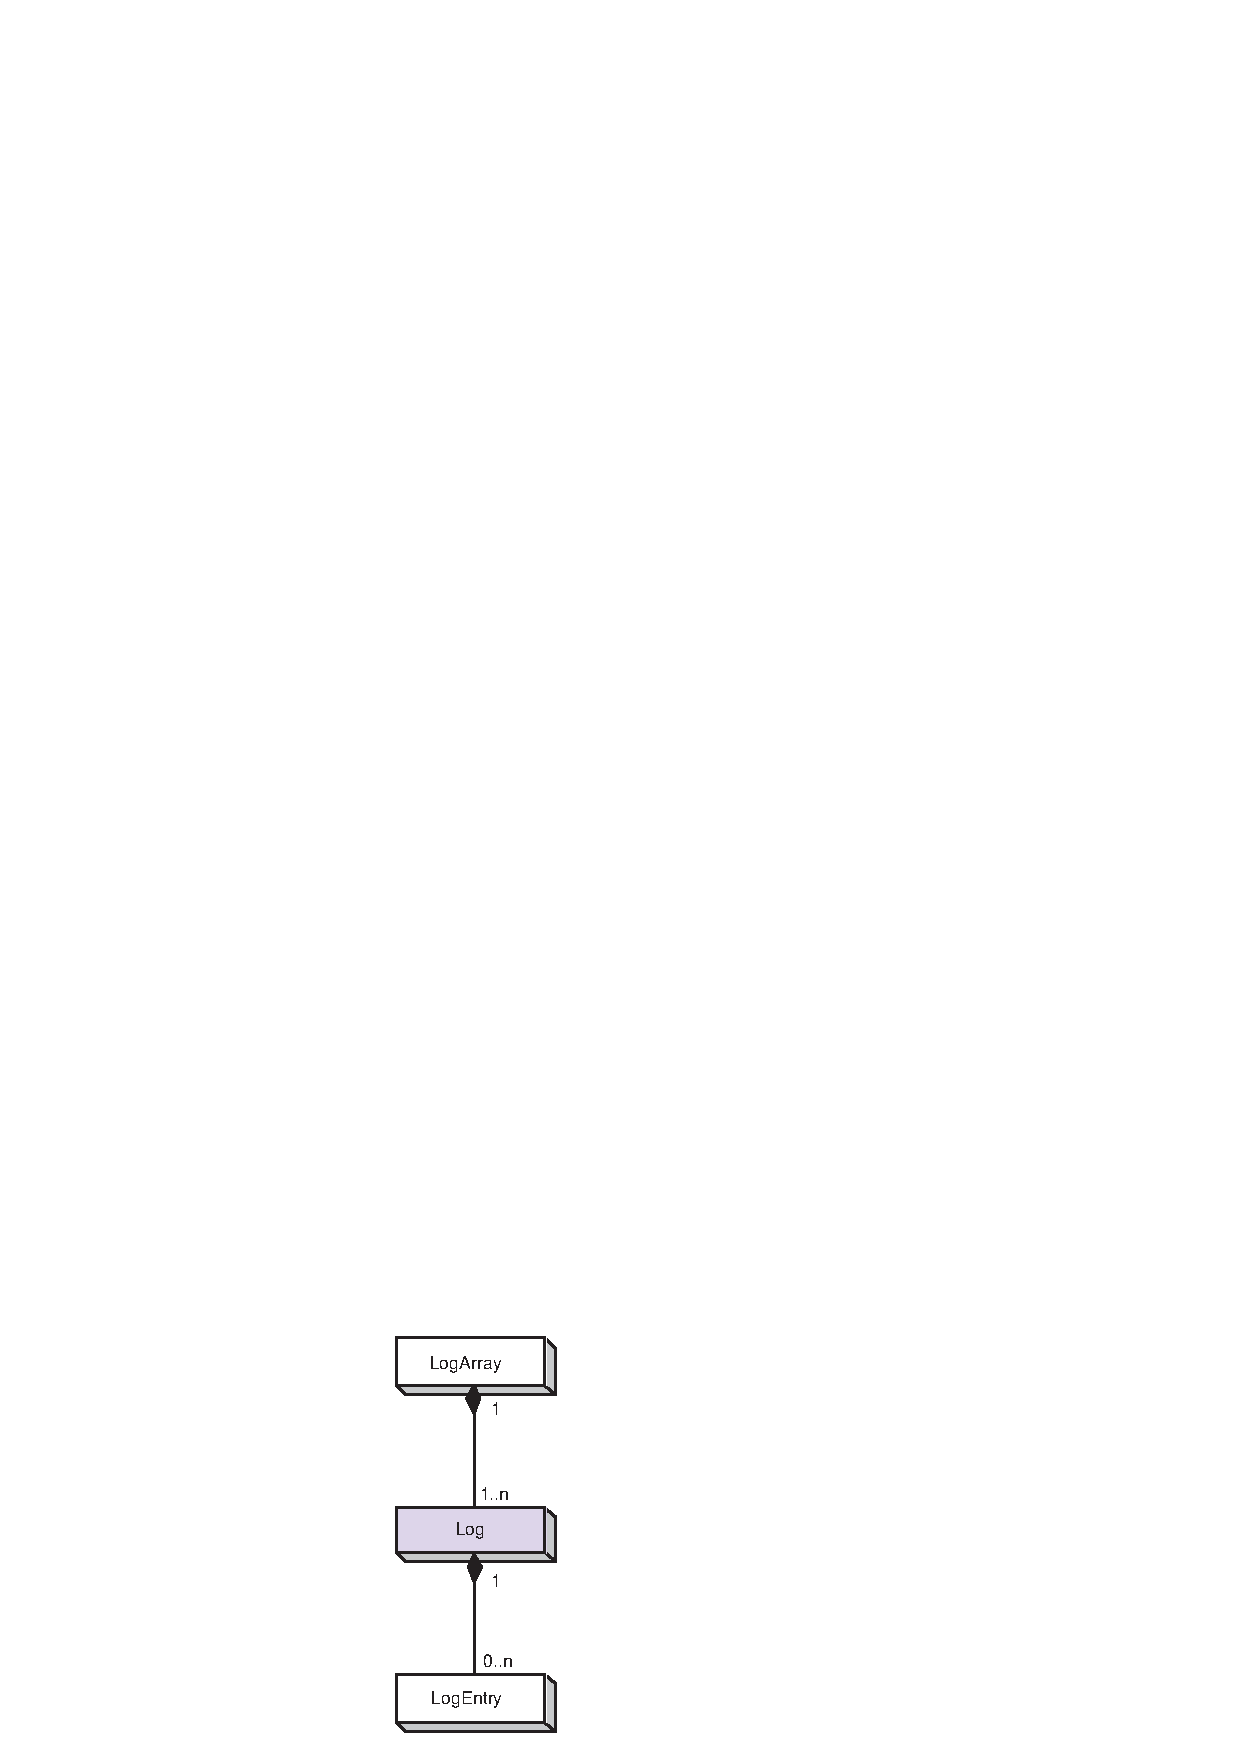
\includegraphics{Log_obj}   
\end{center}


\subsection{Class API}
%                **** IMPORTANT NOTICE *****
% This LaTeX file has been automatically produced by ProTeX v. 1.1
% Any changes made to this file will likely be lost next time
% this file is regenerated from its source. Send questions 
% to Arlindo da Silva, dasilva@gsfc.nasa.gov
 
\setlength{\oldparskip}{\parskip}
\setlength{\parskip}{1.5ex}
\setlength{\oldparindent}{\parindent}
\setlength{\parindent}{0pt}
\setlength{\oldbaselineskip}{\baselineskip}
\setlength{\baselineskip}{11pt}
 
%--------------------- SHORT-HAND MACROS ----------------------
\def\bv{\begin{verbatim}}
\def\ev{\end{verbatim}}
\def\be{\begin{equation}}
\def\ee{\end{equation}}
\def\bea{\begin{eqnarray}}
\def\eea{\end{eqnarray}}
\def\bi{\begin{itemize}}
\def\ei{\end{itemize}}
\def\bn{\begin{enumerate}}
\def\en{\end{enumerate}}
\def\bd{\begin{description}}
\def\ed{\end{description}}
\def\({\left (}
\def\){\right )}
\def\[{\left [}
\def\]{\right ]}
\def\<{\left  \langle}
\def\>{\right \rangle}
\def\cI{{\cal I}}
\def\diag{\mathop{\rm diag}}
\def\tr{\mathop{\rm tr}}
%-------------------------------------------------------------

\markboth{Left}{Source File: ESMC\_LogErr.h,  Date: Tue May  5 20:59:27 MDT 2020
}

 
%/////////////////////////////////////////////////////////////
\subsubsection [ESMC\_LogWrite] {ESMC\_LogWrite - Write an entry into the Log file}


  
\bigskip{\sf INTERFACE:}
\begin{verbatim} int ESMC_LogWrite(
   const char msg[], // in
   int msgtype       // in
 );\end{verbatim}{\em RETURN VALUE:}
\begin{verbatim}    Return code; equals ESMF_SUCCESS if there are no errors.\end{verbatim}
{\sf DESCRIPTION:\\ }


  
    Write an entry into the Log file.
  
    The arguments are:
    \begin{description}
    \item[msg]
      The message to be written.
    \item[msgtype]
      The message type.  This flag is documented in section \ref{const:clogmsgflag}
    \end{description}
   
%/////////////////////////////////////////////////////////////
 
\mbox{}\hrulefill\ 
 
\subsubsection [ESMC\_LogSet] {ESMC\_LogSet - Set Log properties}


  
\bigskip{\sf INTERFACE:}
\begin{verbatim} int ESMC_LogSet(
   int flush       // in
 );\end{verbatim}{\em RETURN VALUE:}
\begin{verbatim}    Return code; equals ESMF_SUCCESS if there are no errors.\end{verbatim}
{\sf DESCRIPTION:\\ }


  
    Set Log properties.
  
    The arguments are:
    \begin{description}
    \item[flush]
      If set to ESMF\_TRUE, flush log messages immediately, rather than buffering 
      them. Default is to flush after 10 messages.
    \end{description}
  
%...............................................................
\setlength{\parskip}{\oldparskip}
\setlength{\parindent}{\oldparindent}
\setlength{\baselineskip}{\oldbaselineskip}

%#ifdef STANDALONE
%\section{Glossary}
%\input{LogErr_glos}
%#endif
%#ifdef STANDALONE
%\section{Bibliography}
%\bibliography{comp}
%\bibliographystyle{plain}
%\addcontentsline{toc}{section}{Bibliography}
%#endif
%#include "../Infrastructure/DELayout/doc/DELayout_crefdoc.ctex"
% $Id$
%
% Earth System Modeling Framework
% Copyright 2002-2020, University Corporation for Atmospheric Research,
% Massachusetts Institute of Technology, Geophysical Fluid Dynamics
% Laboratory, University of Michigan, National Centers for Environmental
% Prediction, Los Alamos National Laboratory, Argonne National Laboratory,
% NASA Goddard Space Flight Center.
% Licensed under the University of Illinois-NCSA License.
\bodytext{BGCOLOR=white LINK=#083194 VLINK=#21004A}
%============================================================================
% VM Class
%============================================================================
\section{VM Class}
\subsection{Description}
% $Id$
%
% Earth System Modeling Framework
% Copyright 2002-2020, University Corporation for Atmospheric Research, 
% Massachusetts Institute of Technology, Geophysical Fluid Dynamics 
% Laboratory, University of Michigan, National Centers for Environmental 
% Prediction, Los Alamos National Laboratory, Argonne National Laboratory, 
% NASA Goddard Space Flight Center.
% Licensed under the University of Illinois-NCSA License.

%TODO: This file started as an exact copy of the Fortran version of this file.
%TODO: Changes were made to correctly reflect the current status of the C API.
%TODO: Eventually this file should be removed again and replaced by a single
%TODO: generic version that can be included for both Fortran and C refdocs.

The ESMF VM (Virtual Machine) class is a generic representation of hardware and system software resources. There is exactly one VM object per ESMF Component, providing the execution environment for the Component code. The VM class handles all resource management tasks for the Component class and provides a description of the underlying configuration of the compute resources used by a Component.

In addition to resource description and management, the VM class offers the lowest level of ESMF communication methods. The VM communication calls are very similar to MPI. Data references in VM communication calls must be provided as raw, language-specific, one-dimensional, contiguous data arrays. The similarity between VM and MPI communication calls is striking and there are many equivalent point-to-point and collective communication calls. However, unlike MPI, the VM communication calls support communication between threaded PETs in a completely transparent fashion.

Many ESMF applications do not interact with the VM class directly very much. The  resource management aspect is wrapped completely transparent into the ESMF Component concept. Often the only reason that user code queries a Component
object for the associated VM object is to inquire about resource information, such as the {\tt localPet} or the {\tt petCount}. Further, for most applications the use of higher level communication APIs, such as provided by Array and Field, are much more convenient than using the low level VM communication calls.

The basic elements of a VM are called PETs, which stands for Persistent Execution Threads. These are equivalent to OS threads with a lifetime of at least that of the associated component. All VM functionality is expressed in terms of PETs. In the simplest, and most common case, a PET is equivalent to an MPI process. However, ESMF also supports multi-threading, where multiple PETs run as Pthreads inside the same virtual address space (VAS).

%\subsection{Constants}
%#ifdef STANDALONE
%\input{VM_options}
%#elif defined(1)
%\input{../Infrastructure/VM/doc/VM_options}
%#endif
%\subsection{Use and Examples}
%% $Id$

The concept of the ESMF Virtual Machine (VM) is so fundamental to the framework that every ESMF application uses it. However, for many user applications the VM class is transparently hidden behind the ESMF Component concept and higher data classes (e.g. Array, Field). The interaction between user code and VM is often only indirect. The following examples provide an overview of where the VM class can come into play in user code.

%%                **** IMPORTANT NOTICE *****
% This LaTeX file has been automatically produced by ProTeX v. 1.1
% Any changes made to this file will likely be lost next time
% this file is regenerated from its source. Send questions 
% to Arlindo da Silva, dasilva@gsfc.nasa.gov
 
\setlength{\oldparskip}{\parskip}
\setlength{\parskip}{1.5ex}
\setlength{\oldparindent}{\parindent}
\setlength{\parindent}{0pt}
\setlength{\oldbaselineskip}{\baselineskip}
\setlength{\baselineskip}{11pt}
 
%--------------------- SHORT-HAND MACROS ----------------------
\def\bv{\begin{verbatim}}
\def\ev{\end{verbatim}}
\def\be{\begin{equation}}
\def\ee{\end{equation}}
\def\bea{\begin{eqnarray}}
\def\eea{\end{eqnarray}}
\def\bi{\begin{itemize}}
\def\ei{\end{itemize}}
\def\bn{\begin{enumerate}}
\def\en{\end{enumerate}}
\def\bd{\begin{description}}
\def\ed{\end{description}}
\def\({\left (}
\def\){\right )}
\def\[{\left [}
\def\]{\right ]}
\def\<{\left  \langle}
\def\>{\right \rangle}
\def\cI{{\cal I}}
\def\diag{\mathop{\rm diag}}
\def\tr{\mathop{\rm tr}}
%-------------------------------------------------------------

\markboth{Left}{Source File: ESMF\_VMDefaultBasicsEx.F90,  Date: Tue May  5 20:59:29 MDT 2020
}

 
%/////////////////////////////////////////////////////////////

  
   \subsubsection{Global VM}
  
   This complete example program demonstrates the simplest ESMF application, 
   consisting of only a main program without any Components. The global
   VM, which is automatically created during the {\tt ESMF\_Initialize()} call,
   is obtained using two different methods. First the global VM will be returned
   by {\tt ESMF\_Initialize()} if the optional {\tt vm} argument is specified.
   The example uses the VM object obtained this way to call the VM print method.
   Second, the global VM can be obtained anywhere in the user application using
   the {\tt ESMF\_VMGetGlobal()} call. The identical VM is returned and several
   VM query methods are called to inquire about the associated resources.
   
%/////////////////////////////////////////////////////////////

 \begin{verbatim}
program ESMF_VMDefaultBasicsEx
#include "ESMF.h"

  use ESMF
  use ESMF_TestMod
  
  implicit none
  
  ! local variables
  integer:: rc
  type(ESMF_VM):: vm
  integer:: localPet, petCount, peCount, ssiId, vas
 
\end{verbatim}
 
%/////////////////////////////////////////////////////////////

 \begin{verbatim}
  call ESMF_Initialize(vm=vm, defaultlogfilename="VMDefaultBasicsEx.Log", &
                    logkindflag=ESMF_LOGKIND_MULTI, rc=rc)
  ! Providing the optional vm argument to ESMF_Initialize() is one way of
  ! obtaining the global VM.
 
\end{verbatim}
 
%/////////////////////////////////////////////////////////////

 \begin{verbatim}
  call ESMF_VMPrint(vm, rc=rc)
 
\end{verbatim}
 
%/////////////////////////////////////////////////////////////

 \begin{verbatim}
  call ESMF_VMGetGlobal(vm=vm, rc=rc)
  ! Calling ESMF_VMGetGlobal() anywhere in the user application is the other
  ! way to obtain the global VM object.
 
\end{verbatim}
 
%/////////////////////////////////////////////////////////////

 \begin{verbatim}
  call ESMF_VMGet(vm, localPet=localPet, petCount=petCount, peCount=peCount, &
    rc=rc)
  ! The VM object contains information about the associated resources. If the
  ! user code requires this information it must query the VM object.
 
\end{verbatim}
 
%/////////////////////////////////////////////////////////////

 \begin{verbatim}
  print *, "This PET is localPet: ", localPet
  print *, "of a total of ",petCount," PETs in this VM."
  print *, "There are ", peCount," PEs referenced by this VM"

  call ESMF_VMGet(vm, localPet, peCount=peCount, ssiId=ssiId, vas=vas, rc=rc)
 
\end{verbatim}
 
%/////////////////////////////////////////////////////////////

 \begin{verbatim}
  print *, "This PET is executing in virtual address space (VAS) ", vas
  print *, "located on single system image (SSI) ", ssiId
  print *, "and is associated with ", peCount, " PEs."

 
\end{verbatim}
 
%/////////////////////////////////////////////////////////////

 \begin{verbatim}
end program
 
\end{verbatim}

%...............................................................
\setlength{\parskip}{\oldparskip}
\setlength{\parindent}{\oldparindent}
\setlength{\baselineskip}{\oldbaselineskip}

%%                **** IMPORTANT NOTICE *****
% This LaTeX file has been automatically produced by ProTeX v. 1.1
% Any changes made to this file will likely be lost next time
% this file is regenerated from its source. Send questions 
% to Arlindo da Silva, dasilva@gsfc.nasa.gov
 
\setlength{\oldparskip}{\parskip}
\setlength{\parskip}{1.5ex}
\setlength{\oldparindent}{\parindent}
\setlength{\parindent}{0pt}
\setlength{\oldbaselineskip}{\baselineskip}
\setlength{\baselineskip}{11pt}
 
%--------------------- SHORT-HAND MACROS ----------------------
\def\bv{\begin{verbatim}}
\def\ev{\end{verbatim}}
\def\be{\begin{equation}}
\def\ee{\end{equation}}
\def\bea{\begin{eqnarray}}
\def\eea{\end{eqnarray}}
\def\bi{\begin{itemize}}
\def\ei{\end{itemize}}
\def\bn{\begin{enumerate}}
\def\en{\end{enumerate}}
\def\bd{\begin{description}}
\def\ed{\end{description}}
\def\({\left (}
\def\){\right )}
\def\[{\left [}
\def\]{\right ]}
\def\<{\left  \langle}
\def\>{\right \rangle}
\def\cI{{\cal I}}
\def\diag{\mathop{\rm diag}}
\def\tr{\mathop{\rm tr}}
%-------------------------------------------------------------

\markboth{Left}{Source File: ESMF\_VMGetMPICommunicatorEx.F90,  Date: Tue May  5 20:59:29 MDT 2020
}

 
%/////////////////////////////////////////////////////////////

  
   \subsubsection{Getting the MPI Communicator from an VM object}
  
   Sometimes user code requires access to the MPI communicator, e.g. to support
   legacy code that contains explict MPI communication calls. The correct way of
   wrapping such code into ESMF is to obtain the MPI intra-communicator out of
   the VM object. In order not to interfere with ESMF communications it is
   advisable to duplicate the communicator before using it in user-level MPI
   calls. In this example the duplicated communicator is used for a user
   controlled {\tt MPI\_Barrier()}.
   
%/////////////////////////////////////////////////////////////

 \begin{verbatim}
  integer:: mpic
 
\end{verbatim}
 
%/////////////////////////////////////////////////////////////

 \begin{verbatim}
  integer:: mpic2
 
\end{verbatim}
 
%/////////////////////////////////////////////////////////////

 \begin{verbatim}
  call ESMF_VMGet(vm, mpiCommunicator=mpic, rc=rc)
  ! The returned MPI communicator spans the same MPI processes that the VM
  ! is defined on.
 
\end{verbatim}
 
%/////////////////////////////////////////////////////////////

 \begin{verbatim}
  call MPI_Comm_dup(mpic, mpic2, ierr)
  ! Duplicate the MPI communicator not to interfere with ESMF communications.
  ! The duplicate MPI communicator can be used in any MPI call in the user
  ! code. Here the MPI_Barrier() routine is called.
  call MPI_Barrier(mpic2, ierr)
 
\end{verbatim}

%...............................................................
\setlength{\parskip}{\oldparskip}
\setlength{\parindent}{\oldparindent}
\setlength{\baselineskip}{\oldbaselineskip}

%%                **** IMPORTANT NOTICE *****
% This LaTeX file has been automatically produced by ProTeX v. 1.1
% Any changes made to this file will likely be lost next time
% this file is regenerated from its source. Send questions 
% to Arlindo da Silva, dasilva@gsfc.nasa.gov
 
\setlength{\oldparskip}{\parskip}
\setlength{\parskip}{1.5ex}
\setlength{\oldparindent}{\parindent}
\setlength{\parindent}{0pt}
\setlength{\oldbaselineskip}{\baselineskip}
\setlength{\baselineskip}{11pt}
 
%--------------------- SHORT-HAND MACROS ----------------------
\def\bv{\begin{verbatim}}
\def\ev{\end{verbatim}}
\def\be{\begin{equation}}
\def\ee{\end{equation}}
\def\bea{\begin{eqnarray}}
\def\eea{\end{eqnarray}}
\def\bi{\begin{itemize}}
\def\ei{\end{itemize}}
\def\bn{\begin{enumerate}}
\def\en{\end{enumerate}}
\def\bd{\begin{description}}
\def\ed{\end{description}}
\def\({\left (}
\def\){\right )}
\def\[{\left [}
\def\]{\right ]}
\def\<{\left  \langle}
\def\>{\right \rangle}
\def\cI{{\cal I}}
\def\diag{\mathop{\rm diag}}
\def\tr{\mathop{\rm tr}}
%-------------------------------------------------------------

\markboth{Left}{Source File: ESMF\_VMUserMpiEx.F90,  Date: Tue May  5 20:59:29 MDT 2020
}

 
%/////////////////////////////////////////////////////////////

  
   \subsubsection{Nesting ESMF inside a user MPI application}
   \label{vm_inside_user_mpi}
  
   \begin{sloppypar}
   It is possible to nest an ESMF application inside a user application that 
   explicitly calls {\tt MPI\_Init()} and {\tt MPI\_Finalize()}. The
   {\tt ESMF\_Initialize()} call automatically checks whether MPI has already
   been initialized, and if so does not call {\tt MPI\_Init()} internally. 
   On the finalize side, {\tt ESMF\_Finalize()} can be instructed to {\em not}
   call {\tt MPI\_Finalize()}, making it the responsibility of the outer code
   to finalize MPI.
   \end{sloppypar}
   
%/////////////////////////////////////////////////////////////

 \begin{verbatim}
  ! User code initializes MPI.
  call MPI_Init(ierr)
 
\end{verbatim}
 
%/////////////////////////////////////////////////////////////

 \begin{verbatim}
  ! ESMF_Initialize() does not call MPI_Init() if it finds MPI initialized.
  call ESMF_Initialize(defaultlogfilename="VMUserMpiEx.Log", &
    logkindflag=ESMF_LOGKIND_MULTI, rc=rc)
 
\end{verbatim}
 
%/////////////////////////////////////////////////////////////

 \begin{verbatim}
  ! Use ESMF here...
 
\end{verbatim}
 
%/////////////////////////////////////////////////////////////

 \begin{verbatim}
  ! Calling ESMF_Finalize() with endflag=ESMF_END_KEEPMPI instructs ESMF
  ! to keep MPI active.
  call ESMF_Finalize(endflag=ESMF_END_KEEPMPI, rc=rc)
 
\end{verbatim}
 
%/////////////////////////////////////////////////////////////

 \begin{verbatim}
  ! It is the responsibility of the outer user code to finalize MPI.
  call MPI_Finalize(ierr)
 
\end{verbatim}

%...............................................................
\setlength{\parskip}{\oldparskip}
\setlength{\parindent}{\oldparindent}
\setlength{\baselineskip}{\oldbaselineskip}

%%                **** IMPORTANT NOTICE *****
% This LaTeX file has been automatically produced by ProTeX v. 1.1
% Any changes made to this file will likely be lost next time
% this file is regenerated from its source. Send questions 
% to Arlindo da Silva, dasilva@gsfc.nasa.gov
 
\setlength{\oldparskip}{\parskip}
\setlength{\parskip}{1.5ex}
\setlength{\oldparindent}{\parindent}
\setlength{\parindent}{0pt}
\setlength{\oldbaselineskip}{\baselineskip}
\setlength{\baselineskip}{11pt}
 
%--------------------- SHORT-HAND MACROS ----------------------
\def\bv{\begin{verbatim}}
\def\ev{\end{verbatim}}
\def\be{\begin{equation}}
\def\ee{\end{equation}}
\def\bea{\begin{eqnarray}}
\def\eea{\end{eqnarray}}
\def\bi{\begin{itemize}}
\def\ei{\end{itemize}}
\def\bn{\begin{enumerate}}
\def\en{\end{enumerate}}
\def\bd{\begin{description}}
\def\ed{\end{description}}
\def\({\left (}
\def\){\right )}
\def\[{\left [}
\def\]{\right ]}
\def\<{\left  \langle}
\def\>{\right \rangle}
\def\cI{{\cal I}}
\def\diag{\mathop{\rm diag}}
\def\tr{\mathop{\rm tr}}
%-------------------------------------------------------------

\markboth{Left}{Source File: ESMF\_VMUserMpiCommEx.F90,  Date: Tue May  5 20:59:29 MDT 2020
}

 
%/////////////////////////////////////////////////////////////

  
   \subsubsection{Nesting ESMF inside a user MPI application on a subset of MPI ranks}
   \label{vm_nesting_esmf}
  
   \begin{sloppypar}
   The previous example demonstrated that it is possible to nest an ESMF 
   application, i.e. {\tt ESMF\_Initialize()}...{\tt ESMF\_Finalize()} inside
   {\tt MPI\_Init()}...{\tt MPI\_Finalize()}. It is not necessary that all
   MPI ranks enter the ESMF application. The following example shows how the
   user code can pass an MPI communicator to {\tt ESMF\_Initialize()}, and
   enter the ESMF application on a subset of MPI ranks.
   \end{sloppypar}
   
%/////////////////////////////////////////////////////////////

 \begin{verbatim}
  ! User code initializes MPI.
  call MPI_Init(ierr)
 
\end{verbatim}
 
%/////////////////////////////////////////////////////////////

 \begin{verbatim}
  ! User code determines the local rank.
  call MPI_Comm_rank(MPI_COMM_WORLD, rank, ierr)
 
\end{verbatim}
 
%/////////////////////////////////////////////////////////////

 \begin{verbatim}
  ! User code prepares MPI communicator "esmfComm", that allows rank 0 and 1
  ! to be grouped together.
  if (rank < 2) then
    ! first communicator split with color=0
    call MPI_Comm_split(MPI_COMM_WORLD, 0, 0, esmfComm, ierr)
  else
    ! second communicator split with color=1
    call MPI_Comm_split(MPI_COMM_WORLD, 1, 0, esmfComm, ierr)
  endif
 
\end{verbatim}
 
%/////////////////////////////////////////////////////////////

 \begin{verbatim}
  if (rank < 2) then
    ! Only call ESMF_Initialize() on rank 0 and 1, passing the prepared MPI
    ! communicator that spans these ranks.
    call ESMF_Initialize(mpiCommunicator=esmfComm, &
      defaultlogfilename="VMUserMpiCommEx.Log", &
      logkindflag=ESMF_LOGKIND_MULTI, rc=rc)
 
\end{verbatim}
 
%/////////////////////////////////////////////////////////////

 \begin{verbatim}
    ! Use ESMF here...
 
\end{verbatim}
 
%/////////////////////////////////////////////////////////////

 \begin{verbatim}
    ! Calling ESMF_Finalize() with endflag=ESMF_END_KEEPMPI instructs ESMF
    ! to keep MPI active.
    call ESMF_Finalize(endflag=ESMF_END_KEEPMPI, rc=rc)
 
\end{verbatim}
 
%/////////////////////////////////////////////////////////////

 \begin{verbatim}
  else
    ! Ranks 2 and above do non-ESMF work...
 
\end{verbatim}
 
%/////////////////////////////////////////////////////////////

 \begin{verbatim}
  endif
 
\end{verbatim}
 
%/////////////////////////////////////////////////////////////

 \begin{verbatim}
  ! Free the MPI communicator before finalizing MPI.
  call MPI_Comm_free(esmfComm, ierr)
  
  ! It is the responsibility of the outer user code to finalize MPI.
  call MPI_Finalize(ierr)
 
\end{verbatim}

%...............................................................
\setlength{\parskip}{\oldparskip}
\setlength{\parindent}{\oldparindent}
\setlength{\baselineskip}{\oldbaselineskip}

%%                **** IMPORTANT NOTICE *****
% This LaTeX file has been automatically produced by ProTeX v. 1.1
% Any changes made to this file will likely be lost next time
% this file is regenerated from its source. Send questions 
% to Arlindo da Silva, dasilva@gsfc.nasa.gov
 
\setlength{\oldparskip}{\parskip}
\setlength{\parskip}{1.5ex}
\setlength{\oldparindent}{\parindent}
\setlength{\parindent}{0pt}
\setlength{\oldbaselineskip}{\baselineskip}
\setlength{\baselineskip}{11pt}
 
%--------------------- SHORT-HAND MACROS ----------------------
\def\bv{\begin{verbatim}}
\def\ev{\end{verbatim}}
\def\be{\begin{equation}}
\def\ee{\end{equation}}
\def\bea{\begin{eqnarray}}
\def\eea{\end{eqnarray}}
\def\bi{\begin{itemize}}
\def\ei{\end{itemize}}
\def\bn{\begin{enumerate}}
\def\en{\end{enumerate}}
\def\bd{\begin{description}}
\def\ed{\end{description}}
\def\({\left (}
\def\){\right )}
\def\[{\left [}
\def\]{\right ]}
\def\<{\left  \langle}
\def\>{\right \rangle}
\def\cI{{\cal I}}
\def\diag{\mathop{\rm diag}}
\def\tr{\mathop{\rm tr}}
%-------------------------------------------------------------

\markboth{Left}{Source File: ESMF\_VMSendVMRecvEx.F90,  Date: Tue May  5 20:59:29 MDT 2020
}

 
%/////////////////////////////////////////////////////////////

  
   \subsubsection{Communication - Send and Recv}
  
   The VM layer provides MPI-like point-to-point communication. Use 
   {\tt ESMF\_VMSend()} and {\tt ESMF\_VMRecv()} to pass data between two PETs.
   The following code sends data from PET 'src' and receives it on PET 'dst'.
   Both PETs must be part of the same VM.
   
%/////////////////////////////////////////////////////////////

 \begin{verbatim}
  integer, allocatable:: localData(:)
 
\end{verbatim}
 
%/////////////////////////////////////////////////////////////

 \begin{verbatim}
  count = 10
  allocate(localData(count))
  do i=1, count
    localData(i) = localPet*100 + i
  enddo
 
\end{verbatim}
 
%/////////////////////////////////////////////////////////////

 \begin{verbatim}
  if (localPet==src) then
    call ESMF_VMSend(vm, sendData=localData, count=count, dstPet=dst, rc=rc)
  endif
 
\end{verbatim}
 
%/////////////////////////////////////////////////////////////

 \begin{verbatim}
  if (localPet==dst) then
    call ESMF_VMRecv(vm, recvData=localData, count=count, srcPet=src, rc=rc)
  endif
 
\end{verbatim}

%...............................................................
\setlength{\parskip}{\oldparskip}
\setlength{\parindent}{\oldparindent}
\setlength{\baselineskip}{\oldbaselineskip}

%%                **** IMPORTANT NOTICE *****
% This LaTeX file has been automatically produced by ProTeX v. 1.1
% Any changes made to this file will likely be lost next time
% this file is regenerated from its source. Send questions 
% to Arlindo da Silva, dasilva@gsfc.nasa.gov
 
\setlength{\oldparskip}{\parskip}
\setlength{\parskip}{1.5ex}
\setlength{\oldparindent}{\parindent}
\setlength{\parindent}{0pt}
\setlength{\oldbaselineskip}{\baselineskip}
\setlength{\baselineskip}{11pt}
 
%--------------------- SHORT-HAND MACROS ----------------------
\def\bv{\begin{verbatim}}
\def\ev{\end{verbatim}}
\def\be{\begin{equation}}
\def\ee{\end{equation}}
\def\bea{\begin{eqnarray}}
\def\eea{\end{eqnarray}}
\def\bi{\begin{itemize}}
\def\ei{\end{itemize}}
\def\bn{\begin{enumerate}}
\def\en{\end{enumerate}}
\def\bd{\begin{description}}
\def\ed{\end{description}}
\def\({\left (}
\def\){\right )}
\def\[{\left [}
\def\]{\right ]}
\def\<{\left  \langle}
\def\>{\right \rangle}
\def\cI{{\cal I}}
\def\diag{\mathop{\rm diag}}
\def\tr{\mathop{\rm tr}}
%-------------------------------------------------------------

\markboth{Left}{Source File: ESMF\_VMScatterVMGatherEx.F90,  Date: Tue May  5 20:59:29 MDT 2020
}

 
%/////////////////////////////////////////////////////////////

  
   \subsubsection{Communication - Scatter and Gather}
  
   The VM layer provides MPI-like collective communication. {\tt ESMF\_VMScatter()}
   scatters data located on {\tt root} PET across all the PETs of the VM. 
   {\tt ESMF\_VMGather()} provides the opposite operation, gathering data from
   all the PETs of the VM onto {\tt root} PET.
   
%/////////////////////////////////////////////////////////////

 \begin{verbatim}
  integer, allocatable:: array1(:), array2(:)
 
\end{verbatim}
 
%/////////////////////////////////////////////////////////////

 \begin{verbatim}
  ! allocate data arrays
  nsize = 2
  nlen = nsize * petCount
  allocate(array1(nlen))
  allocate(array2(nsize))

  ! prepare data array1
  do i=1, nlen
    array1(i) = localPet * 100 + i
  enddo
 
\end{verbatim}
 
%/////////////////////////////////////////////////////////////

 \begin{verbatim}
  call ESMF_VMScatter(vm, sendData=array1, recvData=array2, count=nsize, &
    rootPet=scatterRoot, rc=rc)
 
\end{verbatim}
 
%/////////////////////////////////////////////////////////////

 \begin{verbatim}
  call ESMF_VMGather(vm, sendData=array2, recvData=array1, count=nsize, &
    rootPet=gatherRoot, rc=rc)
 
\end{verbatim}
 

%...............................................................
\setlength{\parskip}{\oldparskip}
\setlength{\parindent}{\oldparindent}
\setlength{\baselineskip}{\oldbaselineskip}

%%                **** IMPORTANT NOTICE *****
% This LaTeX file has been automatically produced by ProTeX v. 1.1
% Any changes made to this file will likely be lost next time
% this file is regenerated from its source. Send questions 
% to Arlindo da Silva, dasilva@gsfc.nasa.gov
 
\setlength{\oldparskip}{\parskip}
\setlength{\parskip}{1.5ex}
\setlength{\oldparindent}{\parindent}
\setlength{\parindent}{0pt}
\setlength{\oldbaselineskip}{\baselineskip}
\setlength{\baselineskip}{11pt}
 
%--------------------- SHORT-HAND MACROS ----------------------
\def\bv{\begin{verbatim}}
\def\ev{\end{verbatim}}
\def\be{\begin{equation}}
\def\ee{\end{equation}}
\def\bea{\begin{eqnarray}}
\def\eea{\end{eqnarray}}
\def\bi{\begin{itemize}}
\def\ei{\end{itemize}}
\def\bn{\begin{enumerate}}
\def\en{\end{enumerate}}
\def\bd{\begin{description}}
\def\ed{\end{description}}
\def\({\left (}
\def\){\right )}
\def\[{\left [}
\def\]{\right ]}
\def\<{\left  \langle}
\def\>{\right \rangle}
\def\cI{{\cal I}}
\def\diag{\mathop{\rm diag}}
\def\tr{\mathop{\rm tr}}
%-------------------------------------------------------------

\markboth{Left}{Source File: ESMF\_VMAllFullReduceEx.F90,  Date: Tue May  5 20:59:29 MDT 2020
}

 
%/////////////////////////////////////////////////////////////

  
   \subsubsection{Communication - AllReduce and AllFullReduce}
  
   Use {\tt ESMF\_VMAllReduce()} to reduce data distributed across the PETs of a 
   VM into a result vector, returned on all the PETs. Further, use
   {\tt ESMF\_VMAllFullReduce()} to reduce the data into a single scalar returned
   on all PETs.
   
%/////////////////////////////////////////////////////////////

 \begin{verbatim}
  integer, allocatable:: array1(:), array2(:)
 
\end{verbatim}
 
%/////////////////////////////////////////////////////////////

 \begin{verbatim}
  ! allocate data arrays
  nsize = 2
  allocate(array1(nsize))
  allocate(array2(nsize))

  ! prepare data array1
  do i=1, nsize
    array1(i) = localPet * 100 + i
  enddo
 
\end{verbatim}
 
%/////////////////////////////////////////////////////////////

 \begin{verbatim}
  call ESMF_VMAllReduce(vm, sendData=array1, recvData=array2, count=nsize, &
    reduceflag=ESMF_REDUCE_SUM, rc=rc)
  ! Reduce distributed sendData, element by element into recvData and
  ! return it on all the PETs.
 
\end{verbatim}
 
%/////////////////////////////////////////////////////////////

 \begin{verbatim}
  call ESMF_VMAllFullReduce(vm, sendData=array1, recvData=result, &
    count=nsize, reduceflag=ESMF_REDUCE_SUM, rc=rc)
  ! Fully reduce the distributed sendData into a single scalar and
  ! return it in recvData on all PETs.
 
\end{verbatim}

%...............................................................
\setlength{\parskip}{\oldparskip}
\setlength{\parindent}{\oldparindent}
\setlength{\baselineskip}{\oldbaselineskip}

%%                **** IMPORTANT NOTICE *****
% This LaTeX file has been automatically produced by ProTeX v. 1.1
% Any changes made to this file will likely be lost next time
% this file is regenerated from its source. Send questions 
% to Arlindo da Silva, dasilva@gsfc.nasa.gov
 
\setlength{\oldparskip}{\parskip}
\setlength{\parskip}{1.5ex}
\setlength{\oldparindent}{\parindent}
\setlength{\parindent}{0pt}
\setlength{\oldbaselineskip}{\baselineskip}
\setlength{\baselineskip}{11pt}
 
%--------------------- SHORT-HAND MACROS ----------------------
\def\bv{\begin{verbatim}}
\def\ev{\end{verbatim}}
\def\be{\begin{equation}}
\def\ee{\end{equation}}
\def\bea{\begin{eqnarray}}
\def\eea{\end{eqnarray}}
\def\bi{\begin{itemize}}
\def\ei{\end{itemize}}
\def\bn{\begin{enumerate}}
\def\en{\end{enumerate}}
\def\bd{\begin{description}}
\def\ed{\end{description}}
\def\({\left (}
\def\){\right )}
\def\[{\left [}
\def\]{\right ]}
\def\<{\left  \langle}
\def\>{\right \rangle}
\def\cI{{\cal I}}
\def\diag{\mathop{\rm diag}}
\def\tr{\mathop{\rm tr}}
%-------------------------------------------------------------

\markboth{Left}{Source File: ESMF\_VMComponentEx.F90,  Date: Tue May  5 20:59:29 MDT 2020
}

 
%/////////////////////////////////////////////////////////////

  
   \subsubsection{VM and Components}
  
   The following example shows the role that the VM plays in connection with ESMF 
   Components. A single Component is created in the main program. Through the
   optional {\tt petList} argument the driver code specifies that only resources
   associated with PET 0 are given to the {\tt gcomp} object. 
  
   When the Component code is invoked through the standard ESMF Component methods
   Initialize, Run, or Finalize the Component's VM is automatically entered.
   Inside of the user-written Component code the Component VM can be obtained
   by querying the Component object. The VM object will indicate that only a
   single PET is executing the Component code.
   
%/////////////////////////////////////////////////////////////

 \begin{verbatim}
module ESMF_VMComponentEx_gcomp_mod
 
\end{verbatim}
 
%/////////////////////////////////////////////////////////////

 \begin{verbatim}
  recursive subroutine mygcomp_init(gcomp, istate, estate, clock, rc)
    type(ESMF_GridComp)   :: gcomp
    type(ESMF_State)      :: istate, estate
    type(ESMF_Clock)      :: clock
    integer, intent(out)  :: rc

    ! local variables
    type(ESMF_VM):: vm
    
    ! get this Component's vm    
    call ESMF_GridCompGet(gcomp, vm=vm)
    
    ! the VM object contains information about the execution environment of
    ! the Component

    call ESMF_VMPrint(vm, rc=rc)
    
    rc = 0
  end subroutine !--------------------------------------------------------------

  
  recursive subroutine mygcomp_run(gcomp, istate, estate, clock, rc)
    type(ESMF_GridComp)   :: gcomp
    type(ESMF_State)      :: istate, estate
    type(ESMF_Clock)      :: clock
    integer, intent(out)  :: rc
    
    ! local variables
    type(ESMF_VM):: vm
    
    ! get this Component's vm    
    call ESMF_GridCompGet(gcomp, vm=vm)
    
    ! the VM object contains information about the execution environment of
    ! the Component

    call ESMF_VMPrint(vm, rc=rc)
    
    rc = 0
  end subroutine !--------------------------------------------------------------

  recursive subroutine mygcomp_final(gcomp, istate, estate, clock, rc)
    type(ESMF_GridComp)   :: gcomp
    type(ESMF_State)      :: istate, estate
    type(ESMF_Clock)      :: clock
    integer, intent(out)  :: rc
    
    ! local variables
    type(ESMF_VM):: vm
    
    ! get this Component's vm    
    call ESMF_GridCompGet(gcomp, vm=vm)
    
    ! the VM object contains information about the execution environment of
    ! the Component

    call ESMF_VMPrint(vm, rc=rc)
    
    rc = 0
  end subroutine !--------------------------------------------------------------

end module
 
\end{verbatim}
 
%/////////////////////////////////////////////////////////////

 \begin{verbatim}
program ESMF_VMComponentEx
#include "ESMF.h"
  use ESMF
  use ESMF_TestMod
  use ESMF_VMComponentEx_gcomp_mod
  implicit none
  
  ! local variables
 
\end{verbatim}
 
%/////////////////////////////////////////////////////////////

 \begin{verbatim}
  gcomp = ESMF_GridCompCreate(petList=(/0/), rc=rc)
 
\end{verbatim}
 
%/////////////////////////////////////////////////////////////

 \begin{verbatim}
  call ESMF_GridCompSetServices(gcomp, userRoutine=mygcomp_register, rc=rc)
 
\end{verbatim}
 
%/////////////////////////////////////////////////////////////

 \begin{verbatim}
  call ESMF_GridCompInitialize(gcomp, rc=rc)
 
\end{verbatim}
 
%/////////////////////////////////////////////////////////////

 \begin{verbatim}
  call ESMF_GridCompRun(gcomp, rc=rc)
 
\end{verbatim}
 
%/////////////////////////////////////////////////////////////

 \begin{verbatim}
  call ESMF_GridCompFinalize(gcomp, rc=rc)
 
\end{verbatim}
 
%/////////////////////////////////////////////////////////////

 \begin{verbatim}
  call ESMF_GridCompDestroy(gcomp, rc=rc)
 
\end{verbatim}
 
%/////////////////////////////////////////////////////////////

 \begin{verbatim}
  call ESMF_Finalize(rc=rc)
 
\end{verbatim}
 
%/////////////////////////////////////////////////////////////

 \begin{verbatim}
end program
 
\end{verbatim}

%...............................................................
\setlength{\parskip}{\oldparskip}
\setlength{\parindent}{\oldparindent}
\setlength{\baselineskip}{\oldbaselineskip}

%\subsection{Restrictions and Future Work}
%% $Id$

%\subsubsection{Restrictions and Future Work}

\begin{enumerate}

\item {\bf Only array section syntax that leads to contiguous sub sections is supported}. The source and destination arguments in VM communication calls must reference contiguous data arrays. Fortran array sections are not guaranteed to be contiguous in all cases.

\item {\bf Non-blocking {\tt Reduce()} operations {\em not} implemented.} None of the reduce communication calls have an implementation for the non-blocking feature. This affects:
\begin{itemize}
\item {\tt ESMF\_VMAllFullReduce()},
\item {\tt ESMF\_VMAllReduce()},
\item {\tt ESMF\_VMReduce()}.
\end{itemize}

\item {\bf Limitations when using {\tt mpiuni} mode.} In {\tt mpiuni} mode non-blocking communications are limited to one outstanding message per source-destination PET pair. Furthermore, in {\tt mpiuni} mode the message length must be smaller than the internal ESMF buffer size.

\item {\bf Alternative communication paths not accessible.} All user accessible VM communication calls are currently implemented using MPI-1.2. VM's implementation of alternative communication techniques, such as shared memory between threaded PETs and POSIX IPC between PETs located on the same single system image, are currently inaccessible to the user. (One exception to this is the {\tt mpiuni} case for which the VM automatically utilizes a shared memory path.)

\item {\bf Data arrays in VM comm calls are {\em assumed shape} with rank=1.} Currently all dummy arrays in VM comm calls are defined as {\em assumed shape} arrays of rank=1. The motivation for this choice is that the use of assumed shape dummy arrays guards against the Fortran copy in/out problem. However it may not be as flexible as desired from the user perspective. Alternatively all dummy arrays could be defined as {\em assumed size} arrays, as it is done in most MPI implementations, allowing arrays of various rank to be passed into the comm methods. Arrays of higher rank can be passed into the current interfaces using Fortran array syntax. This approach is explained in section \ref{vm_higherrank}.

\end{enumerate}



%\subsection{Design and Implementation Notes}
%% $Id$

%\subsection{Design and Implementation Notes}

The VM class provides an additional layer of abstraction on top of the POSIX machine model, making it suitable for HPC applications. There are four key aspects the VM class deals with.

\begin{enumerate}

\item Encapsulation of hardware and operating system details within the concept of Persistent Execution Threads (PETs).

\item Resource management in terms of PETs with a guard against over-subscription.

\item Topological description of the underlying configuration of the compute resources in terms of PETs.

\item Transparent communication API for point-to-point and collective PET-based primitives, hiding the many different communication channels and offering best possible performance.

\end{enumerate}

\begin{center}
\scalebox{0.6}{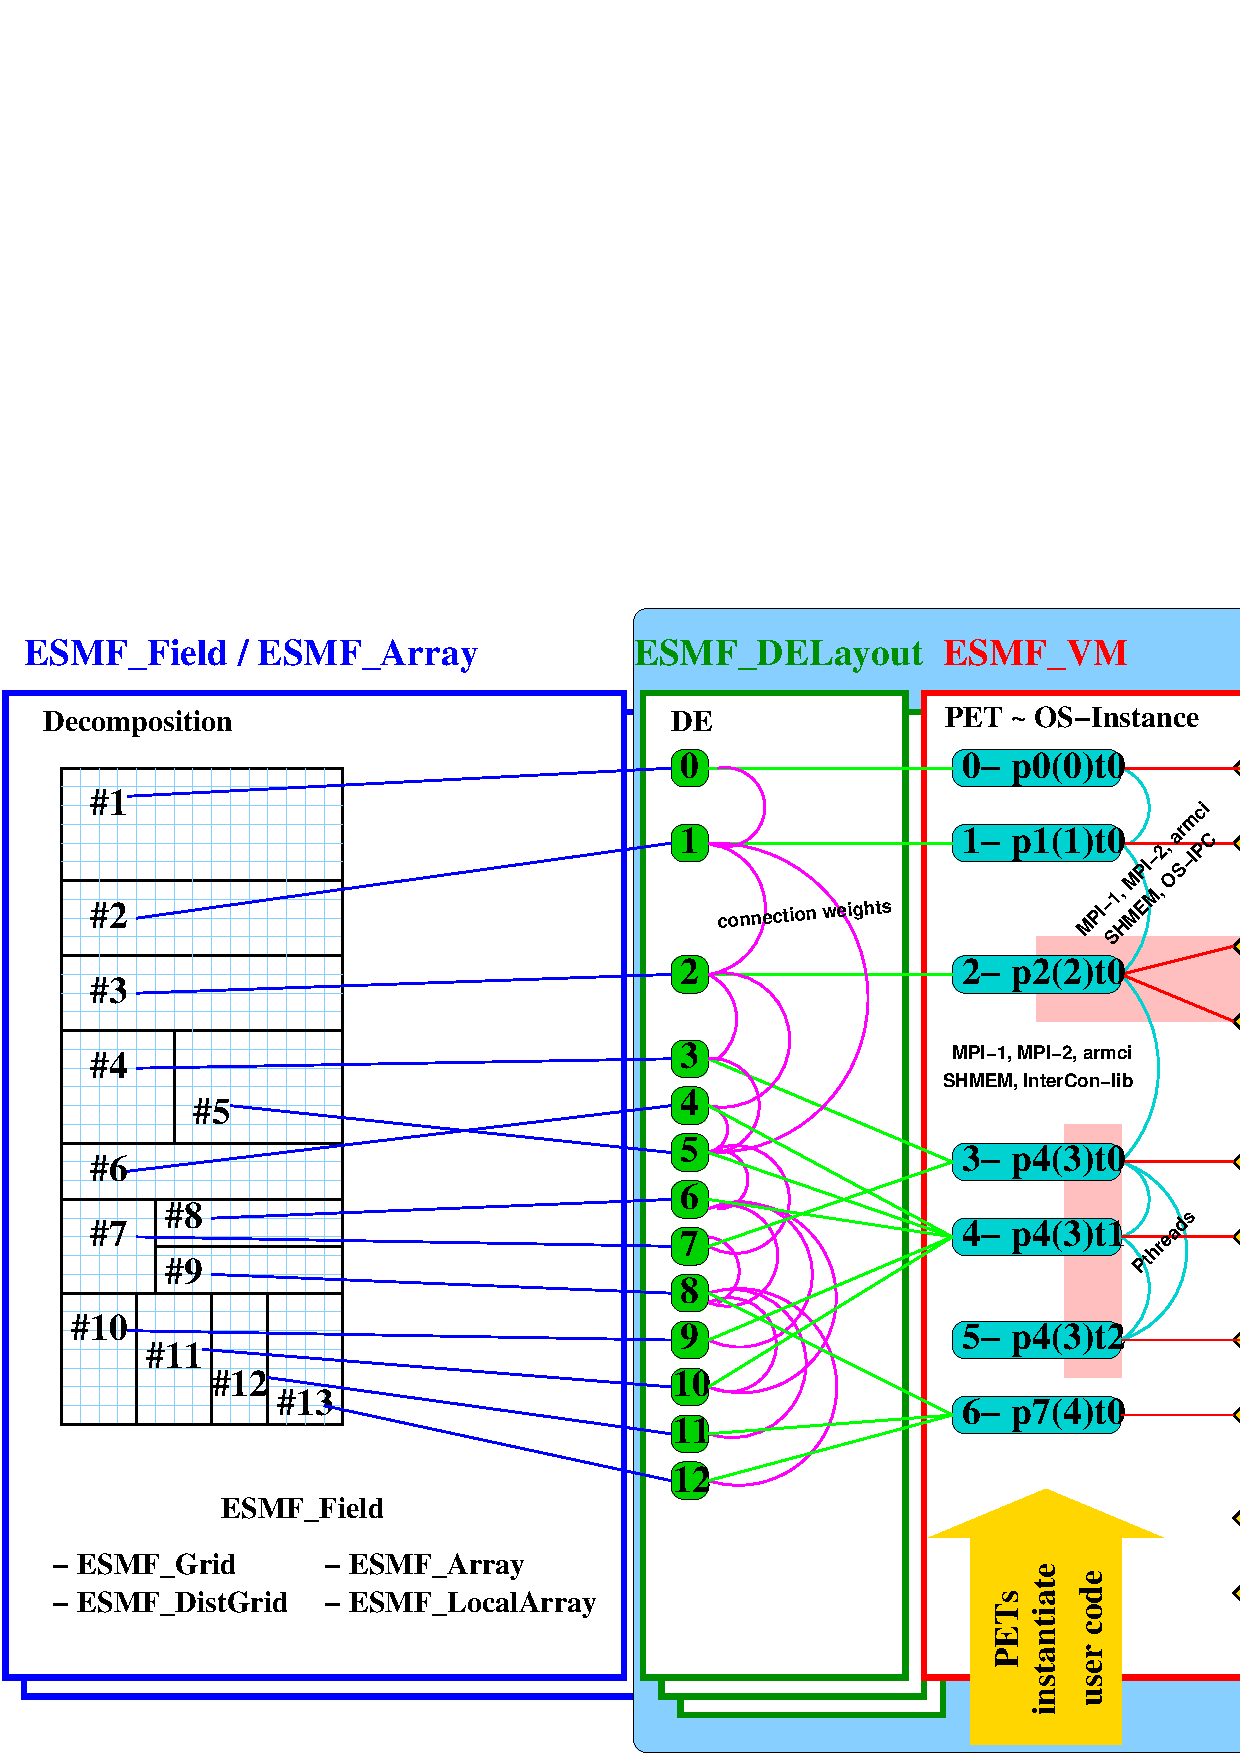
\includegraphics{VM_design}}
\end{center}


{\bf Definition of terms used in the diagram}

\begin{itemize}

\item PE: A processing element (PE) is an alias for the smallest physical processing unit available on a particular hardware platform. In the language of today's microprocessor architecture technology a PE is identical to a core, however, if future microprocessor designs change the smallest physical processing unit the mapping of the PE to actual hardware will change accordingly. Thus the PE layer separates the hardware specific part of the VM from the hardware-independent part. Each PE is labeled with an id number which identifies it uniquely within all of the VM instances of an ESMF application.

\item Core: A Core is the smallest physical processing unit which typically comprises a register set, an integer arithmetic unit, a floating-point unit and various control units. Each Core is labeled with an id number which identifies it uniquely within all of the VM instances of an ESMF application.

\item CPU: The central processing unit (CPU) houses single or multiple cores, providing them with the interface to system memory, interconnects and I/O. Typically the CPU provides some level of caching for the instruction and data streams in and out of the Cores. Cores in a multi-core CPU typically share some caches. Each CPU is labeled with an id number which identifies it uniquely within all of the VM instances of an ESMF application.

\item SSI: A single system image (SSI) spans all the CPUs controlled by a single running instance of the operating system. SMP and NUMA are typical multi-CPU SSI architectures. Each SSI is labeled with an id number which identifies it uniquely within all of the VM instances of an ESMF application.

\item TOE: A thread of execution (TOE) executes an instruction sequence. TOE's come in two flavors: PET and TET.

\item PET: A persistent execution thread (PET) executes an instruction sequence on an associated set of data. The PET has a lifetime at least as long as the associated data set. In ESMF the PET is the central concept of abstraction provided by the VM class. The PETs of an VM object are labeled from 0 to N-1 where N is the total number of PETs in the VM object.

\item TET: A transient execution thread (TET) executes an instruction sequence on an associated set of data. A TET's lifetime might be shorter than that of the associated data set.

\item OS-Instance: The OS-Instance of a TOE describes how a particular TOE is instantiated on the OS level. Using POSIX terminology a TOE will run as a single thread within a single- or multi-threaded process.

\item Pthreads: Communication via the POSIX Thread interface.

\item MPI-1, MPI-2: Communication via MPI standards 1 and 2.

\item armci: Communication via the aggregate remote memory copy interface.

\item SHMEM: Communication via the SHMEM interface.

\item OS-IPC: Communication via the operating system's inter process communication interface. Either POSIX IPC or System V IPC.

\item InterCon-lib: Communication via the interconnect's library native interface. An example is the Elan library for Quadrics.

\end{itemize}

The POSIX machine abstraction, while a very powerful concept, needs augmentation when applied to HPC applications. Key elements of the POSIX abstraction are processes, which provide virtually unlimited resources (memory, I/O, sockets, ...) to possibly multiple threads of execution. Similarly POSIX threads create the illusion that there is virtually unlimited processing power available to each POSIX process. While the POSIX abstraction is very suitable for many multi-user/multi-tasking applications that need to share limited physical resources, it does not directly fit the HPC workload where over-subscription of resources is one of the most expensive modes of operation.

ESMF's virtual machine abstraction is based on the POSIX machine model but holds additional information about the available physical processing units in terms of Processing Elements (PEs). A PE is the smallest physical processing unit and encapsulates the hardware details (Cores, CPUs and SSIs).

There is exactly one physical machine layout for each application, and all VM instances have access to this information. The PE is the smallest processing unit which, in today's microprocessor technology, corresponds to a single Core. Cores are arranged in CPUs which in turn are arranged in SSIs. The setup of the physical machine layout is part of the ESMF initialization process.

On top of the PE concept the key abstraction provided by the VM is the PET. All user code is executed by PETs while OS and hardware details are hidden. The VM class contains a number of methods which allow the user to prescribe how the PETs of a desired virtual machine should be instantiated on the OS level and how they should map onto the hardware. This prescription is kept in a private virtual machine plan object which is created at the same time the associated component is being created. Each time component code is entered through one of the component's registered top--level methods (Initialize/Run/Finalize), the virtual machine plan along with a pointer to the respective user function is used to instantiate the user code on the PETs of the associated VM in form of single- or multi-threaded POSIX processes.

The process of starting, entering, exiting and shutting down a VM is very transparent, all spawning and joining of threads is handled by VM methods "behind the scenes". Furthermore, fundamental synchronization and communication primitives are provided on the PET level through a uniform API, hiding details related to the actual instantiation of the participating PETs.

Within a VM object each PE of the physical machine maps to 0 or 1 PETs. Allowing unassigned PEs provides a means to prevent over-subscription between multiple concurrently running virtual machines. Similarly a maximum of one PET per PE prevents over-subscription within a single VM instance. However, over-subscription is possible by subscribing PETs from different virtual machines to the same PE. This type of over-subscription can be desirable for PETs associated with I/O workloads expected to be used infrequently and to block often on I/O requests.

On the OS level each PET of a VM object is represented by a POSIX thread (Pthread) either belonging to a single-- or multi--threaded process and maps to at least 1 PE of the physical machine, ensuring its execution. Mapping a single PET to multiple PEs provides resources for user--level multi--threading, in which case the user code inquires how many PEs are associated with its PET and if there are multiple PEs available the user code can spawn an equal number of threads (e.g. OpenMP) without risking over-subscription. Typically these user spawned threads are short-lived and used for fine-grained parallelization in form of TETs. All PEs mapped against a single PET must be part of a unique SSI in order to allow user--level multi--threading!

In addition to discovering the physical machine the ESMF initialization process sets up the default global virtual machine. This VM object, which is the ultimate parent of all VMs created during the course of execution, contains as many PETs as there are PEs in the physical machine. All of its PETs are instantiated in form of single-threaded MPI processes and a 1:1 mapping of PETs to PEs is used for the default global VM.

The VM design and implementation is based on the POSIX process and thread model as well as the MPI-1.2 standard. As a consequence of the latter standard the number of processes is static during the course of execution and is determined at start-up. The VM implementation further requires that the user starts up the ESMF application with as many MPI processes as there are PEs in the available physical machine using the platform dependent mechanism to ensure proper process placement. 

All MPI processes participating in a VM are grouped together by means of an MPI\_Group object and their context is defined via an MPI\_Comm object (MPI intra-communicator). The PET local process id within each virtual machine is equal to the MPI\_Comm\_rank in the local MPI\_Comm context whereas the PET process id is equal to the MPI\_Comm\_rank in MPI\_COMM\_WORLD. The PET process id is used within the VM methods to determine the virtual memory space a PET is operating in. 

In order to provide a migration path for legacy MPI-applications the VM offers accessor functions to its MPI\_Comm object. Once obtained this object may be used in explicit user-code MPI calls within the same context.



\subsection{Class API}
%                **** IMPORTANT NOTICE *****
% This LaTeX file has been automatically produced by ProTeX v. 1.1
% Any changes made to this file will likely be lost next time
% this file is regenerated from its source. Send questions 
% to Arlindo da Silva, dasilva@gsfc.nasa.gov
 
\setlength{\oldparskip}{\parskip}
\setlength{\parskip}{1.5ex}
\setlength{\oldparindent}{\parindent}
\setlength{\parindent}{0pt}
\setlength{\oldbaselineskip}{\baselineskip}
\setlength{\baselineskip}{11pt}
 
%--------------------- SHORT-HAND MACROS ----------------------
\def\bv{\begin{verbatim}}
\def\ev{\end{verbatim}}
\def\be{\begin{equation}}
\def\ee{\end{equation}}
\def\bea{\begin{eqnarray}}
\def\eea{\end{eqnarray}}
\def\bi{\begin{itemize}}
\def\ei{\end{itemize}}
\def\bn{\begin{enumerate}}
\def\en{\end{enumerate}}
\def\bd{\begin{description}}
\def\ed{\end{description}}
\def\({\left (}
\def\){\right )}
\def\[{\left [}
\def\]{\right ]}
\def\<{\left  \langle}
\def\>{\right \rangle}
\def\cI{{\cal I}}
\def\diag{\mathop{\rm diag}}
\def\tr{\mathop{\rm tr}}
%-------------------------------------------------------------

\markboth{Left}{Source File: ESMC\_VM.h,  Date: Tue May  5 20:59:29 MDT 2020
}

 
%/////////////////////////////////////////////////////////////
\subsubsection [ESMC\_VMBarrier] {ESMC\_VMBarrier - block calling PETs until all PETS called}


  
\bigskip{\sf INTERFACE:}
\begin{verbatim} int ESMC_VMBarrier(
   ESMC_VM vm                   // in
 );\end{verbatim}{\em RETURN VALUE:}
\begin{verbatim}    Return code; equals ESMF_SUCCESS if there are no errors.\end{verbatim}
{\sf DESCRIPTION:\\ }


  
    Collective {\tt ESMC\_VM} communication call that blocks calling PET until 
    all PETs of the VM context have issued the call.
  
    The arguments are:
    \begin{description}
    \item[vm] 
      Queried {\tt ESMC\_VM} object.
    \item[{[rc]}]
      Return code; equals {\tt ESMF\_SUCCESS} if there are no errors.
    \end{description}
   
%/////////////////////////////////////////////////////////////
 
\mbox{}\hrulefill\ 
 
\subsubsection [ESMC\_VMBroadcast] {ESMC\_VMBroadcast - Broadcast data across the VM}


  
\bigskip{\sf INTERFACE:}
\begin{verbatim} int ESMC_VMBroadcast(ESMC_VM vm,
                   void *bcstData,
                   int count,
                   enum ESMC_TypeKind_Flag *typekind,
                   int rootPet);\end{verbatim}{\em RETURN VALUE:}
\begin{verbatim}    Return code; equals ESMF_SUCCESS if there are no errors.\end{verbatim}
{\sf DESCRIPTION:\\ }


    Collective {\tt ESMC\_VM} communication call that broadcasts a contiguous 
    data array from {\tt rootPet} to all other PETs of the {\tt ESMC\_VM}
    object.
  
    This method is overloaded for:
    {\tt ESMC\_TYPEKIND\_I4}, {\tt ESMC\_TYPEKIND\_I8},
    {\tt ESMC\_TYPEKIND\_R4}, {\tt ESMC\_TYPEKIND\_R8}, 
    {\tt ESMC\_TYPEKIND\_LOGICAL}.
  
    The arguments are:
    \begin{description}
    \item[vm] 
      {\tt ESMC\_VM} object.
    \item[bcstData]
      Contiguous data array. On {\tt rootPet} {\tt bcstData} holds data that
      is to be broadcasted to all other PETs. On all other PETs 
      {\tt bcstData} is used to receive the broadcasted data.
    \item[count] 
      Number of elements in {\tt bcstData}. Must be the same on all PETs.
    \item[typekind]
      The typekind of the data to be reduced. See section 
      \ref{const:ctypekind} for a list of valid typekind options.
    \item[rootPet] 
      PET that holds data that is being broadcast.
    \end{description}
   
%/////////////////////////////////////////////////////////////
 
\mbox{}\hrulefill\ 
 
\subsubsection [ESMC\_VMGet] {ESMC\_VMGet - Get VM internals}


  
\bigskip{\sf INTERFACE:}
\begin{verbatim} int ESMC_VMGet(
   ESMC_VM vm,                   // in
   int *localPet,                // out
   int *petCount,                // out
   int *peCount,                 // out
   MPI_Comm *mpiCommunicator,    // out
   int *pthreadsEnabledFlag,     // out
   int *openMPEnabledFlag        // out
 );\end{verbatim}{\em RETURN VALUE:}
\begin{verbatim}    Return code; equals ESMF_SUCCESS if there are no errors.\end{verbatim}
{\sf DESCRIPTION:\\ }


  
    Get internal information about the specified {\tt ESMC\_VM} object.
  
    The arguments are:
    \begin{description}
    \item[vm] 
      Queried {\tt ESMC\_VM} object.
    \item[{[localPet]}] 
      Upon return this holds the id of the PET that issued this call.
    \item[{[petCount]}]
      Upon return this holds the number of PETs in the specified {\tt ESMC\_VM}
      object.
    \item[{[peCount]}]
      Upon return this holds the number of PEs referenced by the specified
      {\tt ESMC\_VM} object.
    \item[{[mpiCommunicator]}]
      Upon return this holds the MPI intra-communicator used by the 
      specified {\tt ESMC\_VM} object. This communicator may be used for
      user-level MPI communications. It is recommended that the user
      duplicates the communicator via {\tt MPI\_Comm\_Dup()} in order to
      prevent any interference with ESMC communications.
    \item[{[pthreadsEnabledFlag]}]
      A return value of '1' indicates that the ESMF library was compiled with
      Pthreads enabled. A return value of '0' indicates that Pthreads are
      disabled in the ESMF library.
    \item[{[openMPEnabledFlag]}]
      A return value of '1' indicates that the ESMF library was compiled with
      OpenMP enabled. A return value of '0' indicates that OpenMP is
      disabled in the ESMF library.
    \item[{[rc]}]
      Return code; equals {\tt ESMF\_SUCCESS} if there are no errors.
    \end{description}
   
%/////////////////////////////////////////////////////////////
 
\mbox{}\hrulefill\ 
 
\subsubsection [ESMC\_VMGetCurrent] {ESMC\_VMGetCurrent - Get current VM}


  
\bigskip{\sf INTERFACE:}
\begin{verbatim} ESMC_VM ESMC_VMGetCurrent(
   int *rc                     // out
 );\end{verbatim}{\em RETURN VALUE:}
\begin{verbatim}    VM object of the current execution context.\end{verbatim}
{\sf DESCRIPTION:\\ }


  
   \begin{sloppypar}
    Get the {\tt ESMC\_VM} object of the current execution context. Calling
    {\tt ESMC\_VMGetCurrent()} within an ESMC Component, will return the
    same VM object as {\tt ESMC\_GridCompGet(..., vm=vm, ...)} or
    {\tt ESMC\_CplCompGet(..., vm=vm, ...)}. 
   \end{sloppypar}
  
    The main purpose of providing {\tt ESMC\_VMGetCurrent()} is to simplify ESMF
    adoption in legacy code. Specifically, code that uses {\tt MPI\_COMM\_WORLD}
    deep within its calling tree can easily be modified to use the correct MPI
    communicator of the current ESMF execution context. The advantage is that
    these modifications are very local, and do not require wide reaching
    interface changes in the legacy code to pass down the ESMF component object,
    or the MPI communicator.
  
    The use of {\tt ESMC\_VMGetCurrent()} is strongly discouraged in newly
    written Component code. Instead, the ESMF Component object should be used as
    the appropriate container of ESMF context information. This object should be
    passed between the subroutines of a Component, and be queried for any
    Component specific information.
  
    Outside of a Component context, i.e. within the driver context, the call
    to {\tt ESMC\_VMGetCurrent()} is identical to {\tt ESMC\_VMGetGlobal()}.
    \newline
  
    The arguments are:
    \begin{description}
    \item[{[rc]}]
      Return code; equals {\tt ESMF\_SUCCESS} if there are no errors.
    \end{description}
   
%/////////////////////////////////////////////////////////////
 
\mbox{}\hrulefill\ 
 
\subsubsection [ESMC\_VMGetGlobal] {ESMC\_VMGetGlobal - Get global VM}


  
\bigskip{\sf INTERFACE:}
\begin{verbatim} ESMC_VM ESMC_VMGetGlobal(
   int *rc                     // out
 );\end{verbatim}{\em RETURN VALUE:}
\begin{verbatim}    VM object of the global execution context.\end{verbatim}
{\sf DESCRIPTION:\\ }


  
    Get the global {\tt ESMC\_VM} object. This is the VM object
    that is created during {\tt ESMC\_Initialize()} and is the ultimate
    parent of all VM objects in an ESMF application. It is identical to the VM
    object returned by {\tt ESMC\_Initialize(..., vm=vm, ...)}.
  
    The {\tt ESMC\_VMGetGlobal()} call provides access to information about the
    global execution context via the global VM. This call is necessary because
    ESMF does not create a global ESMF Component during
    {\tt ESMC\_Initialize()} that could be queried for information about
    the global execution context of an ESMF application.
    
    Usage of {\tt ESMC\_VMGetGlobal()} from within Component code is
    strongly discouraged. ESMF Components should only access their own VM
    objects through Component methods. Global information, if required by
    the Component user code, should be passed down to the Component from the 
    driver through the Component calling interface.
    \newline
  
    The arguments are:
    \begin{description}
    \item[{[rc]}]
      Return code; equals {\tt ESMF\_SUCCESS} if there are no errors.
    \end{description}
   
%/////////////////////////////////////////////////////////////
 
\mbox{}\hrulefill\ 
 
\subsubsection [ESMC\_VMPrint] {ESMC\_VMPrint - Print a VM}


  
\bigskip{\sf INTERFACE:}
\begin{verbatim} int ESMC_VMPrint(
   ESMC_VM vm                // in
 );\end{verbatim}{\em RETURN VALUE:}
\begin{verbatim}    Return code; equals ESMF_SUCCESS if there are no errors.\end{verbatim}
{\sf DESCRIPTION:\\ }


  
    Print internal information of the specified {\tt ESMC\_VM} object.
  
    The arguments are:
    \begin{description}
    \item[vm] 
      {\tt ESMC\_VM} object to be printed.
    \end{description}
   
%/////////////////////////////////////////////////////////////
 
\mbox{}\hrulefill\ 
 
\subsubsection [ESMC\_VMReduce] {ESMC\_VMReduce - Reduce data from across the VM}


  
\bigskip{\sf INTERFACE:}
\begin{verbatim} int ESMC_VMReduce(ESMC_VM vm,
                   void *sendData,
                   void *recvData,
                   int count,
                   enum ESMC_TypeKind_Flag *typekind,
                   enum ESMC_Reduce_Flag *reduceflag,
                   int rootPet);\end{verbatim}{\em RETURN VALUE:}
\begin{verbatim}    Return code; equals ESMF_SUCCESS if there are no errors.\end{verbatim}
{\sf DESCRIPTION:\\ }


  
    Collective {\tt ESMC\_VM} communication call that reduces a contiguous data 
    array across the {\tt ESMC\_VM} object into a contiguous data array of 
    the same <type><kind>. The result array is returned on {\tt rootPet}. 
    Different reduction operations can be specified.
  
    This method is overloaded for:
    {\tt ESMC\_TYPEKIND\_I4}, {\tt ESMC\_TYPEKIND\_I8},
    {\tt ESMC\_TYPEKIND\_R4}, {\tt ESMC\_TYPEKIND\_R8}.
  
    The arguments are:
    \begin{description}
    \item[vm] 
      {\tt ESMC\_VM} object.
    \item[sendData]
      Contiguous data array holding data to be sent. All PETs must specify a
      valid source array.
    \item[recvData] 
      Contiguous data array for data to be received. Only the {\tt recvData}
      array specified by the {\tt rootPet} will be used by this method.
    \item[count] 
      Number of elements in sendData and recvData. Must be the same on all PETs.
    \item[typekind]
      The typekind of the data to be reduced. See section 
      \ref{const:ctypekind} for a list of valid typekind options.
    \item[reduceflag] 
      Reduction operation. See section \ref{const:creduce} for a list of 
      valid reduce operations.
    \item[rootPet] 
      PET on which reduced data is returned.
    \end{description}
  
%...............................................................
\setlength{\parskip}{\oldparskip}
\setlength{\parindent}{\oldparindent}
\setlength{\baselineskip}{\oldbaselineskip}

%#ifdef STANDALONE
%\section{Bibliography}
%\bibliography{comp}
%\bibliographystyle{plain}
%\addcontentsline{toc}{section}{Bibliography}
%#endif
%#include "../Infrastructure/Util/doc/IOUtil_crefdoc.ctex"
\newpage
\part{References}
\bibliography{ESMF}
\bibliographystyle{plain}
%\addcontentsline{toc}{section}{References}
\newpage
\begin{htmlonly}
\addcontentsline{toc}{part}{Appendices}
\end{htmlonly}
\part{Appendices}
% $Id$

\section{Appendix A: Master List of Constants}
\label{const:cmaster}

\subsection{ESMC\_CALKIND}
This flag is documented in section \ref{const:calkindflag_c}.

\subsection{ESMC\_COORDSYS}
This flag is documented in section \ref{const:ccoordsys}.

\subsection{ESMC\_DECOMP}
\label{const:cdecompflag}
{\sf DESCRIPTION:\\}
Indicates how DistGrid elements are decomposed over DEs.

The type of this flag is:

{\tt type(ESMC\_Decomp\_Flag)}

The valid values are:
\begin{description}
\item [ESMC\_DECOMP\_BALANCED]
      Decompose elements as balanced as possible across DEs. The maximum 
      difference in number of elements per DE is 1, with the extra elements on
      the lower DEs.
\item [ESMC\_DECOMP\_CYCLIC]
      Decompose elements cyclically across DEs.
\item [ESMC\_DECOMP\_RESTFIRST]
      Divide elements over DEs. Assign the rest of this division to the first
      DE.
\item [ESMC\_DECOMP\_RESTLAST]
      Divide elements over DEs. Assign the rest of this division to the last DE.
\item [ESMC\_DECOMP\_SYMMEDGEMAX]
      Decompose elements across the DEs in a symmetric fashion. Start with the
      maximum number of elements at the two edge DEs, and assign a decending
      number of elements to the DEs as the center of the decomposition is 
      approached from both sides.
\end{description}

{\tt subsection(ESMC\_ExtrapMethod\_Flag)}
\label{opt:cextrapmethod}
{\sf DESCRIPTION:\\}
Specify which extrapolation method to use on unmapped destination points after 
regridding.

The type of this flag is:

{\tt type(ESMC\_ExtrapMethod\_Flag)}

The valid values are:
\begin{description}
\item [ESMC\_EXTRAPMETHOD\_NONE]
      Indicates that no extrapolation should be done. 
\item [ESMC\_EXTRAPMETHOD\_NEAREST\_STOD]
      Inverse distance weighted average. 
      Here the value of a destination point is the weighted average of the 
      closest N source points. The weight is the reciprocal of the distance of 
      the source point from the destination point raised to a power P. All the
      weights contributing to one destination point are normalized so that they 
      sum to 1.0. The user can choose N and P when using this method, but 
      defaults are also provided.  
\item [ESMC\_EXTRAPMETHOD\_NEAREST\_IDAVG]
      Nearest source to destination. 
      Here each destination point is mapped to the closest source point. A given 
      source point may go to multiple destination points, but no destination 
      point will receive input from more than one source point. 
\end{description}

\subsection{ESMC\_FILEFORMAT}
This flag is documented in section \ref{const:cfileformat}.

{\tt subsection(ESMC\_FileMode\_Flag)}
\label{opt:cfilemode}
{\sf DESCRIPTION:\\}
Specify which mode to use when writing a weight file.

The type of this flag is:

{\tt type(ESMC\_FileMode\_Flag)}

The valid values are:
\begin{description}
\item [ESMC\_FILEMODE\_BASIC]
      Indicates that only the factorList and factorIndexList should be written. 
\item [ESMC\_FILEMODE\_WITHAUX]
      Indicates that grid center coordinates should also be written.
\end{description}

\subsection{ESMC\_GRIDITEM}
This flag is documented in section \ref{const:cgriditem}.

\subsection{ESMC\_GRIDSTATUS}
This flag is documented in section \ref{const:cgridstatus}.

\subsection{ESMC\_INDEX}
\label{const:indexflag}

{\sf DESCRIPTION:\\}
Indicates whether index is local (per DE) or global (per object).

The type of this flag is:

{\tt type(ESMC\_IndexFlag)}

The valid values are:
\begin{description}
\item [ESMC\_INDEX\_DELOCAL]
      Indicates that DE-local index space starts at lower bound 1 for each DE.
\item [ESMC\_INDEX\_GLOBAL]
      Indicates that global indices are used. This means that DE-local index
      space starts at the global lower bound for each DE.
\item [ESMC\_INDEX\_USER]
      Indicates that the DE-local index bounds are explicitly set by the user.
\end{description}

\subsection{ESMC\_LINETYPE}
\label{opt:lineType}

{\sf DESCRIPTION:\\}  This argument allows the user to select the path of the 
line which connects two points on the surface of a sphere.
This in turn controls the path along which distances are calculated and the 
shape of the edges that make up a cell.

The type of this flag is:

{\tt type(ESMC\_LineType\_Flag)}

The valid values are:
\begin{description}
\item [ESMC\_LINETYPE\_CART]
    Cartesian line. When this option is specified distances are calculated in a 
    straight line through the 3D Cartesian space in which the sphere is 
    embedded. Cells are approximated by 3D planes bounded by 3D Cartesian lines 
    between their corner vertices.
    When calculating regrid weights, this line type is currently the default for 
    the following regrid methods: ESMC\_REGRIDMETHOD\_BILINEAR,
    ESMC\_REGRIDMETHOD\_PATCH, ESMC\_REGRIDMETHOD\_NEAREST\_STOD, and 
    ESMC\_REGRIDMETHOD\_NEAREST\_DTOS.
\item [ESMC\_LINETYPE\_GREAT\_CIRCLE]
    Great circle line. When this option is specified distances are calculated 
    along a great circle path (the shortest distance between two points on a 
    sphere surface). Cells are bounded by great circle paths between their 
    corner vertices. When calculating regrid weights, this line type is 
    currently the default for the following regrid method: 
    ESMC\_REGRIDMETHOD\_CONSERVE.
\end{description}


\subsection{ESMC\_LOGKIND}
This flag is documented in section \ref{const:clogkindflag}.

\subsection{ESMC\_LOGMSG}
This flag is documented in section \ref{const:clogmsgflag}.

\subsection{ESMC\_MESHELEMTYPE}
This flag is documented in section \ref{const:cmeshelemtype}.

\subsection{ESMF\_METHOD}
\label{const:cmethod}

{\sf DESCRIPTION:\\}  
Specify standard ESMF Component method.

The type of this flag is:

{\tt type(ESMF\_Method\_Flag)}

The valid values are:
\begin{description}
\item [ESMF\_METHOD\_FINALIZE]
      Finalize method.
\item [ESMF\_METHOD\_INITIALIZE]
      Initialize method.
\item [ESMF\_METHOD\_READRESTART]
      ReadRestart method.
\item [ESMF\_METHOD\_RUN]
      Run method.
\item [ESMF\_METHOD\_WRITERESTART]
      WriteRestart method.
\end{description}

\subsection{ESMC\_POLEKIND}
This flag is documented in section \ref{const:cpolekind}.

\subsection{ESMC\_REDUCE}
\label{const:creduce}
{\sf DESCRIPTION:\\}
Indicates reduce operation.

The type of this flag is:

{\tt type(ESMC\_Reduce\_Flag)}

The valid values are:
\begin{description}
\item [ESMC\_REDUCE\_SUM]
      Use arithmetic sum to add all data elements.
\item [ESMC\_REDUCE\_MIN]
      Determine the minimum of all data elements.
\item [ESMC\_REDUCE\_MAX]
      Determine the maximum of all data elements.
\end{description}

\subsection{ESMC\_REGION}
\label{const:cregion}
{\sf DESCRIPTION:\\}
Specifies various regions in the data layout of an Array or Field object.

The type of this flag is:

{\tt type(ESMC\_Region\_Flag)}

The valid values are:
\begin{description}
\item [ESMC\_REGION\_TOTAL]
      Total allocated memory.
\item [ESMC\_REGION\_SELECT]
      Region of operation-specific elements.
\item [ESMC\_REGION\_EMPTY]
      The empty region contains no elements.
\end{description}

\subsection{ESMC\_REGRIDMETHOD}
This flag is documented in section \ref{opt:cregridmethod}.

\subsection{ESMC\_STAGGERLOC}
This flag is documented in section \ref{const:cstaggerloc}.

\subsection{ESMC\_TYPEKIND}
\label{const:ctypekind}

{\sf DESCRIPTION:\\}
Named constants used to indicate type and kind combinations supported by the
overloaded ESMC interfaces. The corresponding Fortran kind-parameter constants 
are described in the ESMF\_TYPEKIND section of Appendices of the ESMF Fortran 
reference manual.

The type of these named constants is:

{\tt type(ESMC\_TypeKind\_Flag)}

The named constants are:
\begin{description}
\item [ESMC\_TYPEKIND\_I1]
      Indicates 1 byte integer. \newline 
      (Only available if ESMF was built with 
      {\tt ESMF\_NO\_INTEGER\_1\_BYTE = FALSE}. This is {\em not} the default.)
\item [ESMC\_TYPEKIND\_I2]
      Indicates 2 byte integer. \newline
      (Only available if ESMF was built with 
      {\tt ESMF\_NO\_INTEGER\_2\_BYTE = FALSE}. This is {\em not} the default.)
\item [ESMC\_TYPEKIND\_I4]
      Indicates 4 byte integer.
\item [ESMC\_TYPEKIND\_I8]
      Indicates 8 byte integer.
\item [ESMC\_TYPEKIND\_R4]
      Indicates 4 byte real.
\item [ESMC\_TYPEKIND\_R8]
      Indicates 8 byte real.
\end{description}

\subsection{ESMC\_UNMAPPEDACTION}
\label{const:unmappedaction}
{\sf DESCRIPTION:\\}
Indicates what action to take with respect to unmapped destination points
and the entries of the sparse matrix that correspond to these points.

The type of this flag is:

{\tt type(ESMC\_UnmappedAction\_Flag)}

The valid values are:
\begin{description}
	\item[ESMC\_UNMAPPEDACTION\_ERROR]
	An error is issued when there exist destination points in a regridding
	operation that are not mapped by corresponding source points.
	\item[ESMC\_UNMAPPEDACTION\_IGNORE]
	Destination points which do not have corresponding source points are 
	ignored and zeros are used for the entries of the sparse matrix
	that is generated.
\end{description}


% $Id$
%
% Earth System Modeling Framework
% Copyright 2002-2020, University Corporation for Atmospheric Research,
% Massachusetts Institute of Technology, Geophysical Fluid Dynamics
% Laboratory, University of Michigan, National Centers for Environmental
% Prediction, Los Alamos National Laboratory, Argonne National Laboratory,
% NASA Goddard Space Flight Center.
% Licensed under the University of Illinois-NCSA License.

\section{Appendix B:  A Brief Introduction to UML}

The schematic below shows the Unified Modeling Language (UML) notation 
for the class diagrams presented in this {\it Reference Manual}.  For 
more on UML, see references such as {\it The Unified Modeling Language 
Reference Manual}, Rumbaugh et al, \cite{uml}.


\begin{center}
\scalebox{0.8}{\includegraphics{Appendix_uml}}
\end{center}



% $Id$
%
% Earth System Modeling Framework
% Copyright 2002-2020, University Corporation for Atmospheric Research,
% Massachusetts Institute of Technology, Geophysical Fluid Dynamics
% Laboratory, University of Michigan, National Centers for Environmental
% Prediction, Los Alamos National Laboratory, Argonne National Laboratory,
% NASA Goddard Space Flight Center.
% Licensed under the University of Illinois-NCSA License.

\section{Appendix C:  ESMF Error Return Codes}
\label{appendix_esmf_error_codes}

The tables below show the possible error return codes for Fortran and
C methods. 

%                **** IMPORTANT NOTICE *****
% This LaTeX file has been automatically produced by ProTeX v. 1.1
% Any changes made to this file will likely be lost next time
% this file is regenerated from its source. Send questions 
% to Arlindo da Silva, dasilva@gsfc.nasa.gov
 
\setlength{\oldparskip}{\parskip}
\setlength{\parskip}{1.5ex}
\setlength{\oldparindent}{\parindent}
\setlength{\parindent}{0pt}
\setlength{\oldbaselineskip}{\baselineskip}
\setlength{\baselineskip}{11pt}
 
%--------------------- SHORT-HAND MACROS ----------------------
\def\bv{\begin{verbatim}}
\def\ev{\end{verbatim}}
\def\be{\begin{equation}}
\def\ee{\end{equation}}
\def\bea{\begin{eqnarray}}
\def\eea{\end{eqnarray}}
\def\bi{\begin{itemize}}
\def\ei{\end{itemize}}
\def\bn{\begin{enumerate}}
\def\en{\end{enumerate}}
\def\bd{\begin{description}}
\def\ed{\end{description}}
\def\({\left (}
\def\){\right )}
\def\[{\left [}
\def\]{\right ]}
\def\<{\left  \langle}
\def\>{\right \rangle}
\def\cI{{\cal I}}
\def\diag{\mathop{\rm diag}}
\def\tr{\mathop{\rm tr}}
%-------------------------------------------------------------

\markboth{Left}{Source File: ESMC\_ReturnCodes.h,  Date: Tue May  5 20:59:25 MDT 2020
}

 
%/////////////////////////////////////////////////////////////

 \begin{verbatim}
 
 =====================================
 Fortran Symmetric Return Codes 1-500
 =====================================
 
  ESMF_SUCCESS               0
  ESMF_RC_OBJ_BAD            1
  ESMF_RC_OBJ_INIT           2
  ESMF_RC_OBJ_CREATE         3
  ESMF_RC_OBJ_COR            4
  ESMF_RC_OBJ_WRONG          5
  ESMF_RC_ARG_BAD            6
  ESMF_RC_ARG_RANK           7
  ESMF_RC_ARG_SIZE           8
  ESMF_RC_ARG_VALUE          9
  ESMF_RC_ARG_DUP           10
  ESMF_RC_ARG_SAMETYPE      11
  ESMF_RC_ARG_SAMECOMM      12
  ESMF_RC_ARG_INCOMP        13
  ESMF_RC_ARG_CORRUPT       14
  ESMF_RC_ARG_WRONG         15
  ESMF_RC_ARG_OUTOFRANGE    16
  ESMF_RC_ARG_OPT           17
  ESMF_RC_NOT_IMPL          18
  ESMF_RC_FILE_OPEN         19
  ESMF_RC_FILE_CREATE       20
  ESMF_RC_FILE_READ         21
  ESMF_RC_FILE_WRITE        22
  ESMF_RC_FILE_UNEXPECTED   23
  ESMF_RC_FILE_CLOSE        24
  ESMF_RC_FILE_ACTIVE       25
  ESMF_RC_PTR_NULL          26
  ESMF_RC_PTR_BAD           27
  ESMF_RC_PTR_NOTALLOC      28
  ESMF_RC_PTR_ISALLOC       29
  ESMF_RC_MEM               30
  ESMF_RC_MEM_ALLOCATE      31
  ESMF_RC_MEM_DEALLOCATE    32
  ESMF_RC_MEMC              33
  ESMF_RC_DUP_NAME          34
  ESMF_RC_LONG_NAME         35
  ESMF_RC_LONG_STR          36
  ESMF_RC_COPY_FAIL         37
  ESMF_RC_DIV_ZERO          38
  ESMF_RC_CANNOT_GET        39
  ESMF_RC_CANNOT_SET        40
  ESMF_RC_NOT_FOUND         41
  ESMF_RC_NOT_VALID         42
  ESMF_RC_INTNRL_LIST       43
  ESMF_RC_INTNRL_INCONS     44
  ESMF_RC_INTNRL_BAD        45
  ESMF_RC_SYS               46
  ESMF_RC_BUSY              47
  ESMF_RC_LIB               48
  ESMF_RC_LIB_NOT_PRESENT   49
  ESMF_RC_ATTR_UNUSED       50
  ESMF_RC_OBJ_NOT_CREATED   51
  ESMF_RC_OBJ_DELETED       52
  ESMF_RC_NOT_SET           53
  ESMF_RC_VAL_WRONG         54
  ESMF_RC_VAL_ERRBOUND      55
  ESMF_RC_VAL_OUTOFRANGE    56
  ESMF_RC_ATTR_NOTSET       57
  ESMF_RC_ATTR_WRONGTYPE    58
  ESMF_RC_ATTR_ITEMSOFF     59
  ESMF_RC_ATTR_LINK         60
  ESMF_RC_BUFFER_SHORT      61
  ESMF_RC_TIMEOUT           62
  ESMF_RC_FILE_EXISTS       63
  ESMF_RC_FILE_NOTDIR       64
  ESMF_RC_MOAB_ERROR        65
  ESMF_RC_NOOP              66
  ESMF_RC_NETCDF_ERROR      67
 
 68-499 reserved for future Fortran symmetric return code definitions
 
 =====================================
 C/C++ Symmetric Return Codes 501-999
 =====================================
 
  ESMC_RC_OBJ_BAD          501
  ESMC_RC_OBJ_INIT         502
  ESMC_RC_OBJ_CREATE       503
  ESMC_RC_OBJ_COR          504
  ESMC_RC_OBJ_WRONG        505
  ESMC_RC_ARG_BAD          506
  ESMC_RC_ARG_RANK         507
  ESMC_RC_ARG_SIZE         508
  ESMC_RC_ARG_VALUE        509
  ESMC_RC_ARG_DUP          510
  ESMC_RC_ARG_SAMETYPE     511
  ESMC_RC_ARG_SAMECOMM     512
  ESMC_RC_ARG_INCOMP       513
  ESMC_RC_ARG_CORRUPT      514
  ESMC_RC_ARG_WRONG        515
  ESMC_RC_ARG_OUTOFRANGE   516
  ESMC_RC_ARG_OPT          517
  ESMC_RC_NOT_IMPL         518
  ESMC_RC_FILE_OPEN        519
  ESMC_RC_FILE_CREATE      520
  ESMC_RC_FILE_READ        521
  ESMC_RC_FILE_WRITE       522
  ESMC_RC_FILE_UNEXPECTED  523
  ESMC_RC_FILE_CLOSE       524
  ESMC_RC_FILE_ACTIVE      525
  ESMC_RC_PTR_NULL         526
  ESMC_RC_PTR_BAD          527
  ESMC_RC_PTR_NOTALLOC     528
  ESMC_RC_PTR_ISALLOC      529
  ESMC_RC_MEM              530
  ESMC_RC_MEM_ALLOCATE     531
  ESMC_RC_MEM_DEALLOCATE   532
  ESMC_RC_MEMC             533
  ESMC_RC_DUP_NAME         534
  ESMC_RC_LONG_NAME        535
  ESMC_RC_LONG_STR         536
  ESMC_RC_COPY_FAIL        537
  ESMC_RC_DIV_ZERO         538
  ESMC_RC_CANNOT_GET       539
  ESMC_RC_CANNOT_SET       540
  ESMC_RC_NOT_FOUND        541
  ESMC_RC_NOT_VALID        542
  ESMC_RC_INTNRL_LIST      543
  ESMC_RC_INTNRL_INCONS    544
  ESMC_RC_INTNRL_BAD       545
  ESMC_RC_SYS              546
  ESMC_RC_BUSY             547
  ESMC_RC_LIB              548
  ESMC_RC_LIB_NOT_PRESENT  549
  ESMC_RC_ATTR_UNUSED      550
  ESMC_RC_OBJ_NOT_CREATED  551
  ESMC_RC_OBJ_DELETED      552
  ESMC_RC_NOT_SET          553
  ESMC_RC_VAL_WRONG        554
  ESMC_RC_VAL_ERRBOUND     555
  ESMC_RC_VAL_OUTOFRANGE   556
  ESMC_RC_ATTR_NOTSET      557
  ESMC_RC_ATTR_WRONGTYPE   558
  ESMC_RC_ATTR_ITEMSOFF    559
  ESMC_RC_ATTR_LINK        560
  ESMC_RC_BUFFER_SHORT     561
  ESMC_RC_TIMEOUT          562
  ESMC_RC_FILE_EXISTS      563
  ESMC_RC_FILE_NOTDIR      564
  ESMC_RC_MOAB_ERROR       565
  ESMC_RC_NOOP             566
  ESMC_RC_NETCDF_ERROR     567
 
 568-999 reserved for future C/C++ symmetric return code definitions
 
 =====================================
 C/C++ Non-symmetric Return Codes 1000
 =====================================
 
  ESMC_RC_OPTARG_BAD      1000
 
 \end{verbatim}
%...............................................................
\setlength{\parskip}{\oldparskip}
\setlength{\parindent}{\oldparindent}
\setlength{\baselineskip}{\oldbaselineskip}



\end{document}
